\documentclass[twoside]{book}

% Packages required by doxygen
\usepackage{fixltx2e}
\usepackage{calc}
\usepackage{doxygen}
\usepackage[export]{adjustbox} % also loads graphicx
\usepackage{graphicx}
\usepackage[utf8]{inputenc}
\usepackage{makeidx}
\usepackage{multicol}
\usepackage{multirow}
\PassOptionsToPackage{warn}{textcomp}
\usepackage{textcomp}
\usepackage[nointegrals]{wasysym}
\usepackage[table]{xcolor}

% Font selection
\usepackage[T1]{fontenc}
\usepackage[scaled=.90]{helvet}
\usepackage{courier}
\usepackage{amssymb}
\usepackage{sectsty}
\renewcommand{\familydefault}{\sfdefault}
\allsectionsfont{%
  \fontseries{bc}\selectfont%
  \color{darkgray}%
}
\renewcommand{\DoxyLabelFont}{%
  \fontseries{bc}\selectfont%
  \color{darkgray}%
}
\newcommand{\+}{\discretionary{\mbox{\scriptsize$\hookleftarrow$}}{}{}}

% Page & text layout
\usepackage{geometry}
\geometry{%
  a4paper,%
  top=2.5cm,%
  bottom=2.5cm,%
  left=2.5cm,%
  right=2.5cm%
}
\tolerance=750
\hfuzz=15pt
\hbadness=750
\setlength{\emergencystretch}{15pt}
\setlength{\parindent}{0cm}
\setlength{\parskip}{3ex plus 2ex minus 2ex}
\makeatletter
\renewcommand{\paragraph}{%
  \@startsection{paragraph}{4}{0ex}{-1.0ex}{1.0ex}{%
    \normalfont\normalsize\bfseries\SS@parafont%
  }%
}
\renewcommand{\subparagraph}{%
  \@startsection{subparagraph}{5}{0ex}{-1.0ex}{1.0ex}{%
    \normalfont\normalsize\bfseries\SS@subparafont%
  }%
}
\makeatother

% Headers & footers
\usepackage{fancyhdr}
\pagestyle{fancyplain}
\fancyhead[LE]{\fancyplain{}{\bfseries\thepage}}
\fancyhead[CE]{\fancyplain{}{}}
\fancyhead[RE]{\fancyplain{}{\bfseries\leftmark}}
\fancyhead[LO]{\fancyplain{}{\bfseries\rightmark}}
\fancyhead[CO]{\fancyplain{}{}}
\fancyhead[RO]{\fancyplain{}{\bfseries\thepage}}
\fancyfoot[LE]{\fancyplain{}{}}
\fancyfoot[CE]{\fancyplain{}{}}
\fancyfoot[RE]{\fancyplain{}{\bfseries\scriptsize Generated by Doxygen }}
\fancyfoot[LO]{\fancyplain{}{\bfseries\scriptsize Generated by Doxygen }}
\fancyfoot[CO]{\fancyplain{}{}}
\fancyfoot[RO]{\fancyplain{}{}}
\renewcommand{\footrulewidth}{0.4pt}
\renewcommand{\chaptermark}[1]{%
  \markboth{#1}{}%
}
\renewcommand{\sectionmark}[1]{%
  \markright{\thesection\ #1}%
}

% Indices & bibliography
\usepackage{natbib}
\usepackage[titles]{tocloft}
\setcounter{tocdepth}{3}
\setcounter{secnumdepth}{5}
\makeindex

% Hyperlinks (required, but should be loaded last)
\usepackage{ifpdf}
\ifpdf
  \usepackage[pdftex,pagebackref=true]{hyperref}
\else
  \usepackage[ps2pdf,pagebackref=true]{hyperref}
\fi
\hypersetup{%
  colorlinks=true,%
  linkcolor=blue,%
  citecolor=blue,%
  unicode%
}

% Custom commands
\newcommand{\clearemptydoublepage}{%
  \newpage{\pagestyle{empty}\cleardoublepage}%
}

\usepackage{caption}
\captionsetup{labelsep=space,justification=centering,font={bf},singlelinecheck=off,skip=4pt,position=top}

%===== C O N T E N T S =====

\begin{document}

% Titlepage & ToC
\hypersetup{pageanchor=false,
             bookmarksnumbered=true,
             pdfencoding=unicode
            }
\pagenumbering{alph}
\begin{titlepage}
\vspace*{7cm}
\begin{center}%
{\Large U\+I\+U\+Cscaipy2 }\\
\vspace*{1cm}
{\large Generated by Doxygen 1.8.14}\\
\end{center}
\end{titlepage}
\clearemptydoublepage
\pagenumbering{roman}
\tableofcontents
\clearemptydoublepage
\pagenumbering{arabic}
\hypersetup{pageanchor=true}

%--- Begin generated contents ---
\chapter{Namespace Index}
\section{Namespace List}
Here is a list of all namespaces with brief descriptions\+:\begin{DoxyCompactList}
\item\contentsline{section}{\mbox{\hyperlink{namespacepysc2}{pysc2}} }{\pageref{namespacepysc2}}{}
\item\contentsline{section}{\mbox{\hyperlink{namespacepysc2_1_1agents}{pysc2.\+agents}} }{\pageref{namespacepysc2_1_1agents}}{}
\item\contentsline{section}{\mbox{\hyperlink{namespacepysc2_1_1agents_1_1base__agent}{pysc2.\+agents.\+base\+\_\+agent}} }{\pageref{namespacepysc2_1_1agents_1_1base__agent}}{}
\item\contentsline{section}{\mbox{\hyperlink{namespacepysc2_1_1agents_1_1random__agent}{pysc2.\+agents.\+random\+\_\+agent}} }{\pageref{namespacepysc2_1_1agents_1_1random__agent}}{}
\item\contentsline{section}{\mbox{\hyperlink{namespacepysc2_1_1agents_1_1scripted__agent}{pysc2.\+agents.\+scripted\+\_\+agent}} }{\pageref{namespacepysc2_1_1agents_1_1scripted__agent}}{}
\item\contentsline{section}{\mbox{\hyperlink{namespacepysc2_1_1bin}{pysc2.\+bin}} }{\pageref{namespacepysc2_1_1bin}}{}
\item\contentsline{section}{\mbox{\hyperlink{namespacepysc2_1_1bin_1_1agent}{pysc2.\+bin.\+agent}} }{\pageref{namespacepysc2_1_1bin_1_1agent}}{}
\item\contentsline{section}{\mbox{\hyperlink{namespacepysc2_1_1bin_1_1agent__remote}{pysc2.\+bin.\+agent\+\_\+remote}} }{\pageref{namespacepysc2_1_1bin_1_1agent__remote}}{}
\item\contentsline{section}{\mbox{\hyperlink{namespacepysc2_1_1bin_1_1gen__actions}{pysc2.\+bin.\+gen\+\_\+actions}} }{\pageref{namespacepysc2_1_1bin_1_1gen__actions}}{}
\item\contentsline{section}{\mbox{\hyperlink{namespacepysc2_1_1bin_1_1gen__units}{pysc2.\+bin.\+gen\+\_\+units}} }{\pageref{namespacepysc2_1_1bin_1_1gen__units}}{}
\item\contentsline{section}{\mbox{\hyperlink{namespacepysc2_1_1bin_1_1gen__versions}{pysc2.\+bin.\+gen\+\_\+versions}} }{\pageref{namespacepysc2_1_1bin_1_1gen__versions}}{}
\item\contentsline{section}{\mbox{\hyperlink{namespacepysc2_1_1bin_1_1map__list}{pysc2.\+bin.\+map\+\_\+list}} }{\pageref{namespacepysc2_1_1bin_1_1map__list}}{}
\item\contentsline{section}{\mbox{\hyperlink{namespacepysc2_1_1bin_1_1play}{pysc2.\+bin.\+play}} }{\pageref{namespacepysc2_1_1bin_1_1play}}{}
\item\contentsline{section}{\mbox{\hyperlink{namespacepysc2_1_1bin_1_1play__vs__agent}{pysc2.\+bin.\+play\+\_\+vs\+\_\+agent}} }{\pageref{namespacepysc2_1_1bin_1_1play__vs__agent}}{}
\item\contentsline{section}{\mbox{\hyperlink{namespacepysc2_1_1bin_1_1replay__actions}{pysc2.\+bin.\+replay\+\_\+actions}} }{\pageref{namespacepysc2_1_1bin_1_1replay__actions}}{}
\item\contentsline{section}{\mbox{\hyperlink{namespacepysc2_1_1bin_1_1replay__info}{pysc2.\+bin.\+replay\+\_\+info}} }{\pageref{namespacepysc2_1_1bin_1_1replay__info}}{}
\item\contentsline{section}{\mbox{\hyperlink{namespacepysc2_1_1bin_1_1run__tests}{pysc2.\+bin.\+run\+\_\+tests}} }{\pageref{namespacepysc2_1_1bin_1_1run__tests}}{}
\item\contentsline{section}{\mbox{\hyperlink{namespacepysc2_1_1bin_1_1valid__actions}{pysc2.\+bin.\+valid\+\_\+actions}} }{\pageref{namespacepysc2_1_1bin_1_1valid__actions}}{}
\item\contentsline{section}{\mbox{\hyperlink{namespacepysc2_1_1env}{pysc2.\+env}} }{\pageref{namespacepysc2_1_1env}}{}
\item\contentsline{section}{\mbox{\hyperlink{namespacepysc2_1_1env_1_1available__actions__printer}{pysc2.\+env.\+available\+\_\+actions\+\_\+printer}} }{\pageref{namespacepysc2_1_1env_1_1available__actions__printer}}{}
\item\contentsline{section}{\mbox{\hyperlink{namespacepysc2_1_1env_1_1base__env__wrapper}{pysc2.\+env.\+base\+\_\+env\+\_\+wrapper}} }{\pageref{namespacepysc2_1_1env_1_1base__env__wrapper}}{}
\item\contentsline{section}{\mbox{\hyperlink{namespacepysc2_1_1env_1_1environment}{pysc2.\+env.\+environment}} }{\pageref{namespacepysc2_1_1env_1_1environment}}{}
\item\contentsline{section}{\mbox{\hyperlink{namespacepysc2_1_1env_1_1lan__sc2__env}{pysc2.\+env.\+lan\+\_\+sc2\+\_\+env}} }{\pageref{namespacepysc2_1_1env_1_1lan__sc2__env}}{}
\item\contentsline{section}{\mbox{\hyperlink{namespacepysc2_1_1env_1_1mock__sc2__env}{pysc2.\+env.\+mock\+\_\+sc2\+\_\+env}} }{\pageref{namespacepysc2_1_1env_1_1mock__sc2__env}}{}
\item\contentsline{section}{\mbox{\hyperlink{namespacepysc2_1_1env_1_1mock__sc2__env__comparison__test}{pysc2.\+env.\+mock\+\_\+sc2\+\_\+env\+\_\+comparison\+\_\+test}} }{\pageref{namespacepysc2_1_1env_1_1mock__sc2__env__comparison__test}}{}
\item\contentsline{section}{\mbox{\hyperlink{namespacepysc2_1_1env_1_1mock__sc2__env__test}{pysc2.\+env.\+mock\+\_\+sc2\+\_\+env\+\_\+test}} }{\pageref{namespacepysc2_1_1env_1_1mock__sc2__env__test}}{}
\item\contentsline{section}{\mbox{\hyperlink{namespacepysc2_1_1env_1_1remote__sc2__env}{pysc2.\+env.\+remote\+\_\+sc2\+\_\+env}} }{\pageref{namespacepysc2_1_1env_1_1remote__sc2__env}}{}
\item\contentsline{section}{\mbox{\hyperlink{namespacepysc2_1_1env_1_1run__loop}{pysc2.\+env.\+run\+\_\+loop}} }{\pageref{namespacepysc2_1_1env_1_1run__loop}}{}
\item\contentsline{section}{\mbox{\hyperlink{namespacepysc2_1_1env_1_1sc2__env}{pysc2.\+env.\+sc2\+\_\+env}} }{\pageref{namespacepysc2_1_1env_1_1sc2__env}}{}
\item\contentsline{section}{\mbox{\hyperlink{namespacepysc2_1_1lib}{pysc2.\+lib}} }{\pageref{namespacepysc2_1_1lib}}{}
\item\contentsline{section}{\mbox{\hyperlink{namespacepysc2_1_1lib_1_1actions}{pysc2.\+lib.\+actions}} }{\pageref{namespacepysc2_1_1lib_1_1actions}}{}
\item\contentsline{section}{\mbox{\hyperlink{namespacepysc2_1_1lib_1_1colors}{pysc2.\+lib.\+colors}} }{\pageref{namespacepysc2_1_1lib_1_1colors}}{}
\item\contentsline{section}{\mbox{\hyperlink{namespacepysc2_1_1lib_1_1features}{pysc2.\+lib.\+features}} }{\pageref{namespacepysc2_1_1lib_1_1features}}{}
\item\contentsline{section}{\mbox{\hyperlink{namespacepysc2_1_1lib_1_1features__test}{pysc2.\+lib.\+features\+\_\+test}} }{\pageref{namespacepysc2_1_1lib_1_1features__test}}{}
\item\contentsline{section}{\mbox{\hyperlink{namespacepysc2_1_1lib_1_1gfile}{pysc2.\+lib.\+gfile}} }{\pageref{namespacepysc2_1_1lib_1_1gfile}}{}
\item\contentsline{section}{\mbox{\hyperlink{namespacepysc2_1_1lib_1_1metrics}{pysc2.\+lib.\+metrics}} }{\pageref{namespacepysc2_1_1lib_1_1metrics}}{}
\item\contentsline{section}{\mbox{\hyperlink{namespacepysc2_1_1lib_1_1named__array}{pysc2.\+lib.\+named\+\_\+array}} }{\pageref{namespacepysc2_1_1lib_1_1named__array}}{}
\item\contentsline{section}{\mbox{\hyperlink{namespacepysc2_1_1lib_1_1named__array__test}{pysc2.\+lib.\+named\+\_\+array\+\_\+test}} }{\pageref{namespacepysc2_1_1lib_1_1named__array__test}}{}
\item\contentsline{section}{\mbox{\hyperlink{namespacepysc2_1_1lib_1_1point}{pysc2.\+lib.\+point}} }{\pageref{namespacepysc2_1_1lib_1_1point}}{}
\item\contentsline{section}{\mbox{\hyperlink{namespacepysc2_1_1lib_1_1point__flag}{pysc2.\+lib.\+point\+\_\+flag}} }{\pageref{namespacepysc2_1_1lib_1_1point__flag}}{}
\item\contentsline{section}{\mbox{\hyperlink{namespacepysc2_1_1lib_1_1point__test}{pysc2.\+lib.\+point\+\_\+test}} }{\pageref{namespacepysc2_1_1lib_1_1point__test}}{}
\item\contentsline{section}{\mbox{\hyperlink{namespacepysc2_1_1lib_1_1protocol}{pysc2.\+lib.\+protocol}} }{\pageref{namespacepysc2_1_1lib_1_1protocol}}{}
\item\contentsline{section}{\mbox{\hyperlink{namespacepysc2_1_1lib_1_1remote__controller}{pysc2.\+lib.\+remote\+\_\+controller}} }{\pageref{namespacepysc2_1_1lib_1_1remote__controller}}{}
\item\contentsline{section}{\mbox{\hyperlink{namespacepysc2_1_1lib_1_1renderer__human}{pysc2.\+lib.\+renderer\+\_\+human}} }{\pageref{namespacepysc2_1_1lib_1_1renderer__human}}{}
\item\contentsline{section}{\mbox{\hyperlink{namespacepysc2_1_1lib_1_1run__parallel}{pysc2.\+lib.\+run\+\_\+parallel}} }{\pageref{namespacepysc2_1_1lib_1_1run__parallel}}{}
\item\contentsline{section}{\mbox{\hyperlink{namespacepysc2_1_1lib_1_1run__parallel__test}{pysc2.\+lib.\+run\+\_\+parallel\+\_\+test}} }{\pageref{namespacepysc2_1_1lib_1_1run__parallel__test}}{}
\item\contentsline{section}{\mbox{\hyperlink{namespacepysc2_1_1lib_1_1sc__process}{pysc2.\+lib.\+sc\+\_\+process}} }{\pageref{namespacepysc2_1_1lib_1_1sc__process}}{}
\item\contentsline{section}{\mbox{\hyperlink{namespacepysc2_1_1lib_1_1static__data}{pysc2.\+lib.\+static\+\_\+data}} }{\pageref{namespacepysc2_1_1lib_1_1static__data}}{}
\item\contentsline{section}{\mbox{\hyperlink{namespacepysc2_1_1lib_1_1stopwatch}{pysc2.\+lib.\+stopwatch}} }{\pageref{namespacepysc2_1_1lib_1_1stopwatch}}{}
\item\contentsline{section}{\mbox{\hyperlink{namespacepysc2_1_1lib_1_1stopwatch__test}{pysc2.\+lib.\+stopwatch\+\_\+test}} }{\pageref{namespacepysc2_1_1lib_1_1stopwatch__test}}{}
\item\contentsline{section}{\mbox{\hyperlink{namespacepysc2_1_1lib_1_1transform}{pysc2.\+lib.\+transform}} }{\pageref{namespacepysc2_1_1lib_1_1transform}}{}
\item\contentsline{section}{\mbox{\hyperlink{namespacepysc2_1_1lib_1_1units}{pysc2.\+lib.\+units}} }{\pageref{namespacepysc2_1_1lib_1_1units}}{}
\item\contentsline{section}{\mbox{\hyperlink{namespacepysc2_1_1lib_1_1video__writer}{pysc2.\+lib.\+video\+\_\+writer}} }{\pageref{namespacepysc2_1_1lib_1_1video__writer}}{}
\item\contentsline{section}{\mbox{\hyperlink{namespacepysc2_1_1maps}{pysc2.\+maps}} }{\pageref{namespacepysc2_1_1maps}}{}
\item\contentsline{section}{\mbox{\hyperlink{namespacepysc2_1_1maps_1_1ladder}{pysc2.\+maps.\+ladder}} }{\pageref{namespacepysc2_1_1maps_1_1ladder}}{}
\item\contentsline{section}{\mbox{\hyperlink{namespacepysc2_1_1maps_1_1lib}{pysc2.\+maps.\+lib}} }{\pageref{namespacepysc2_1_1maps_1_1lib}}{}
\item\contentsline{section}{\mbox{\hyperlink{namespacepysc2_1_1maps_1_1melee}{pysc2.\+maps.\+melee}} }{\pageref{namespacepysc2_1_1maps_1_1melee}}{}
\item\contentsline{section}{\mbox{\hyperlink{namespacepysc2_1_1maps_1_1mini__games}{pysc2.\+maps.\+mini\+\_\+games}} }{\pageref{namespacepysc2_1_1maps_1_1mini__games}}{}
\item\contentsline{section}{\mbox{\hyperlink{namespacepysc2_1_1run__configs}{pysc2.\+run\+\_\+configs}} }{\pageref{namespacepysc2_1_1run__configs}}{}
\item\contentsline{section}{\mbox{\hyperlink{namespacepysc2_1_1run__configs_1_1lib}{pysc2.\+run\+\_\+configs.\+lib}} }{\pageref{namespacepysc2_1_1run__configs_1_1lib}}{}
\item\contentsline{section}{\mbox{\hyperlink{namespacepysc2_1_1run__configs_1_1platforms}{pysc2.\+run\+\_\+configs.\+platforms}} }{\pageref{namespacepysc2_1_1run__configs_1_1platforms}}{}
\item\contentsline{section}{\mbox{\hyperlink{namespacepysc2_1_1tests}{pysc2.\+tests}} }{\pageref{namespacepysc2_1_1tests}}{}
\item\contentsline{section}{\mbox{\hyperlink{namespacepysc2_1_1tests_1_1dummy__observation}{pysc2.\+tests.\+dummy\+\_\+observation}} }{\pageref{namespacepysc2_1_1tests_1_1dummy__observation}}{}
\item\contentsline{section}{\mbox{\hyperlink{namespacepysc2_1_1tests_1_1dummy__observation__test}{pysc2.\+tests.\+dummy\+\_\+observation\+\_\+test}} }{\pageref{namespacepysc2_1_1tests_1_1dummy__observation__test}}{}
\item\contentsline{section}{\mbox{\hyperlink{namespacepysc2_1_1tests_1_1easy__scripted__test}{pysc2.\+tests.\+easy\+\_\+scripted\+\_\+test}} }{\pageref{namespacepysc2_1_1tests_1_1easy__scripted__test}}{}
\item\contentsline{section}{\mbox{\hyperlink{namespacepysc2_1_1tests_1_1maps__test}{pysc2.\+tests.\+maps\+\_\+test}} }{\pageref{namespacepysc2_1_1tests_1_1maps__test}}{}
\item\contentsline{section}{\mbox{\hyperlink{namespacepysc2_1_1tests_1_1multi__player__env__test}{pysc2.\+tests.\+multi\+\_\+player\+\_\+env\+\_\+test}} }{\pageref{namespacepysc2_1_1tests_1_1multi__player__env__test}}{}
\item\contentsline{section}{\mbox{\hyperlink{namespacepysc2_1_1tests_1_1multi__player__test}{pysc2.\+tests.\+multi\+\_\+player\+\_\+test}} }{\pageref{namespacepysc2_1_1tests_1_1multi__player__test}}{}
\item\contentsline{section}{\mbox{\hyperlink{namespacepysc2_1_1tests_1_1obs__spec__test}{pysc2.\+tests.\+obs\+\_\+spec\+\_\+test}} }{\pageref{namespacepysc2_1_1tests_1_1obs__spec__test}}{}
\item\contentsline{section}{\mbox{\hyperlink{namespacepysc2_1_1tests_1_1observer__test}{pysc2.\+tests.\+observer\+\_\+test}} }{\pageref{namespacepysc2_1_1tests_1_1observer__test}}{}
\item\contentsline{section}{\mbox{\hyperlink{namespacepysc2_1_1tests_1_1ping__test}{pysc2.\+tests.\+ping\+\_\+test}} }{\pageref{namespacepysc2_1_1tests_1_1ping__test}}{}
\item\contentsline{section}{\mbox{\hyperlink{namespacepysc2_1_1tests_1_1protocol__error__test}{pysc2.\+tests.\+protocol\+\_\+error\+\_\+test}} }{\pageref{namespacepysc2_1_1tests_1_1protocol__error__test}}{}
\item\contentsline{section}{\mbox{\hyperlink{namespacepysc2_1_1tests_1_1random__agent__test}{pysc2.\+tests.\+random\+\_\+agent\+\_\+test}} }{\pageref{namespacepysc2_1_1tests_1_1random__agent__test}}{}
\item\contentsline{section}{\mbox{\hyperlink{namespacepysc2_1_1tests_1_1render__test}{pysc2.\+tests.\+render\+\_\+test}} }{\pageref{namespacepysc2_1_1tests_1_1render__test}}{}
\item\contentsline{section}{\mbox{\hyperlink{namespacepysc2_1_1tests_1_1replay__obs__test}{pysc2.\+tests.\+replay\+\_\+obs\+\_\+test}} }{\pageref{namespacepysc2_1_1tests_1_1replay__obs__test}}{}
\item\contentsline{section}{\mbox{\hyperlink{namespacepysc2_1_1tests_1_1utils}{pysc2.\+tests.\+utils}} }{\pageref{namespacepysc2_1_1tests_1_1utils}}{}
\item\contentsline{section}{\mbox{\hyperlink{namespacepysc2_1_1tests_1_1versions__test}{pysc2.\+tests.\+versions\+\_\+test}} }{\pageref{namespacepysc2_1_1tests_1_1versions__test}}{}
\end{DoxyCompactList}

\chapter{Hierarchical Index}
\section{Class Hierarchy}
This inheritance list is sorted roughly, but not completely, alphabetically\+:\begin{DoxyCompactList}
\item a\begin{DoxyCompactList}
\item \contentsline{section}{pysc2.\+lib.\+named\+\_\+array\+\_\+test.\+Bad\+Named\+Tuple}{\pageref{classpysc2_1_1lib_1_1named__array__test_1_1_bad_named_tuple}}{}
\item \contentsline{section}{pysc2.\+lib.\+named\+\_\+array\+\_\+test.\+Test\+Named\+Tuple}{\pageref{classpysc2_1_1lib_1_1named__array__test_1_1_test_named_tuple}}{}
\end{DoxyCompactList}
\item ability\begin{DoxyCompactList}
\item \contentsline{section}{pysc2.\+lib.\+renderer\+\_\+human.\+Past\+Action}{\pageref{classpysc2_1_1lib_1_1renderer__human_1_1_past_action}}{}
\end{DoxyCompactList}
\item ability\+\_\+id\begin{DoxyCompactList}
\item \contentsline{section}{pysc2.\+lib.\+actions.\+Function}{\pageref{classpysc2_1_1lib_1_1actions_1_1_function}}{}
\end{DoxyCompactList}
\item args\begin{DoxyCompactList}
\item \contentsline{section}{pysc2.\+lib.\+actions.\+Function}{\pageref{classpysc2_1_1lib_1_1actions_1_1_function}}{}
\end{DoxyCompactList}
\item Argument\+Parser\begin{DoxyCompactList}
\item \contentsline{section}{pysc2.\+lib.\+point\+\_\+flag.\+Point\+Parser}{\pageref{classpysc2_1_1lib_1_1point__flag_1_1_point_parser}}{}
\end{DoxyCompactList}
\item arguments\begin{DoxyCompactList}
\item \contentsline{section}{pysc2.\+lib.\+actions.\+Function\+Call}{\pageref{classpysc2_1_1lib_1_1actions_1_1_function_call}}{}
\end{DoxyCompactList}
\item avail\+\_\+fn\begin{DoxyCompactList}
\item \contentsline{section}{pysc2.\+lib.\+actions.\+Function}{\pageref{classpysc2_1_1lib_1_1actions_1_1_function}}{}
\end{DoxyCompactList}
\item b\begin{DoxyCompactList}
\item \contentsline{section}{pysc2.\+lib.\+colors.\+Color}{\pageref{classpysc2_1_1lib_1_1colors_1_1_color}}{}
\item \contentsline{section}{pysc2.\+lib.\+named\+\_\+array\+\_\+test.\+Bad\+Named\+Tuple}{\pageref{classpysc2_1_1lib_1_1named__array__test_1_1_bad_named_tuple}}{}
\item \contentsline{section}{pysc2.\+lib.\+named\+\_\+array\+\_\+test.\+Test\+Named\+Tuple}{\pageref{classpysc2_1_1lib_1_1named__array__test_1_1_test_named_tuple}}{}
\item \contentsline{section}{pysc2.\+lib.\+point.\+Rect}{\pageref{classpysc2_1_1lib_1_1point_1_1_rect}}{}
\end{DoxyCompactList}
\item binary\begin{DoxyCompactList}
\item \contentsline{section}{pysc2.\+run\+\_\+configs.\+lib.\+Version}{\pageref{classpysc2_1_1run__configs_1_1lib_1_1_version}}{}
\end{DoxyCompactList}
\item build\+\_\+queue\+\_\+id\begin{DoxyCompactList}
\item \contentsline{section}{pysc2.\+lib.\+actions.\+Arguments}{\pageref{classpysc2_1_1lib_1_1actions_1_1_arguments}}{}
\end{DoxyCompactList}
\item build\+\_\+version\begin{DoxyCompactList}
\item \contentsline{section}{pysc2.\+run\+\_\+configs.\+lib.\+Version}{\pageref{classpysc2_1_1run__configs_1_1lib_1_1_version}}{}
\end{DoxyCompactList}
\item c\begin{DoxyCompactList}
\item \contentsline{section}{pysc2.\+lib.\+named\+\_\+array\+\_\+test.\+Test\+Named\+Tuple}{\pageref{classpysc2_1_1lib_1_1named__array__test_1_1_test_named_tuple}}{}
\end{DoxyCompactList}
\item camera\begin{DoxyCompactList}
\item \contentsline{section}{pysc2.\+lib.\+features.\+Minimap\+Features}{\pageref{classpysc2_1_1lib_1_1features_1_1_minimap_features}}{}
\end{DoxyCompactList}
\item clip\begin{DoxyCompactList}
\item \contentsline{section}{pysc2.\+lib.\+features.\+Feature}{\pageref{classpysc2_1_1lib_1_1features_1_1_feature}}{}
\end{DoxyCompactList}
\item color\begin{DoxyCompactList}
\item \contentsline{section}{pysc2.\+lib.\+renderer\+\_\+human.\+Past\+Action}{\pageref{classpysc2_1_1lib_1_1renderer__human_1_1_past_action}}{}
\end{DoxyCompactList}
\item control\+\_\+group\+\_\+act\begin{DoxyCompactList}
\item \contentsline{section}{pysc2.\+lib.\+actions.\+Arguments}{\pageref{classpysc2_1_1lib_1_1actions_1_1_arguments}}{}
\end{DoxyCompactList}
\item control\+\_\+group\+\_\+id\begin{DoxyCompactList}
\item \contentsline{section}{pysc2.\+lib.\+actions.\+Arguments}{\pageref{classpysc2_1_1lib_1_1actions_1_1_arguments}}{}
\end{DoxyCompactList}
\item creep\begin{DoxyCompactList}
\item \contentsline{section}{pysc2.\+lib.\+features.\+Minimap\+Features}{\pageref{classpysc2_1_1lib_1_1features_1_1_minimap_features}}{}
\item \contentsline{section}{pysc2.\+lib.\+features.\+Screen\+Features}{\pageref{classpysc2_1_1lib_1_1features_1_1_screen_features}}{}
\end{DoxyCompactList}
\item data\+\_\+version\begin{DoxyCompactList}
\item \contentsline{section}{pysc2.\+run\+\_\+configs.\+lib.\+Version}{\pageref{classpysc2_1_1run__configs_1_1lib_1_1_version}}{}
\end{DoxyCompactList}
\item deadline\begin{DoxyCompactList}
\item \contentsline{section}{pysc2.\+lib.\+renderer\+\_\+human.\+Past\+Action}{\pageref{classpysc2_1_1lib_1_1renderer__human_1_1_past_action}}{}
\end{DoxyCompactList}
\item dict\begin{DoxyCompactList}
\item \contentsline{section}{pysc2.\+lib.\+named\+\_\+array.\+Named\+Dict}{\pageref{classpysc2_1_1lib_1_1named__array_1_1_named_dict}}{}
\end{DoxyCompactList}
\item discount\begin{DoxyCompactList}
\item \contentsline{section}{pysc2.\+env.\+environment.\+Time\+Step}{\pageref{classpysc2_1_1env_1_1environment_1_1_time_step}}{}
\end{DoxyCompactList}
\item effects\begin{DoxyCompactList}
\item \contentsline{section}{pysc2.\+lib.\+features.\+Screen\+Features}{\pageref{classpysc2_1_1lib_1_1features_1_1_screen_features}}{}
\end{DoxyCompactList}
\item Enum\begin{DoxyCompactList}
\item \contentsline{section}{pysc2.\+lib.\+actions.\+Action\+Space}{\pageref{classpysc2_1_1lib_1_1actions_1_1_action_space}}{}
\item \contentsline{section}{pysc2.\+lib.\+features.\+Feature\+Type}{\pageref{classpysc2_1_1lib_1_1features_1_1_feature_type}}{}
\item \contentsline{section}{pysc2.\+lib.\+renderer\+\_\+human.\+Action\+Cmd}{\pageref{classpysc2_1_1lib_1_1renderer__human_1_1_action_cmd}}{}
\end{DoxyCompactList}
\item Exception\begin{DoxyCompactList}
\item \contentsline{section}{pysc2.\+env.\+lan\+\_\+sc2\+\_\+env.\+Restart\+Exception}{\pageref{classpysc2_1_1env_1_1lan__sc2__env_1_1_restart_exception}}{}
\item \contentsline{section}{pysc2.\+env.\+remote\+\_\+sc2\+\_\+env.\+Restart\+Exception}{\pageref{classpysc2_1_1env_1_1remote__sc2__env_1_1_restart_exception}}{}
\item \contentsline{section}{pysc2.\+lib.\+protocol.\+Connection\+Error}{\pageref{classpysc2_1_1lib_1_1protocol_1_1_connection_error}}{}
\item \contentsline{section}{pysc2.\+lib.\+protocol.\+Protocol\+Error}{\pageref{classpysc2_1_1lib_1_1protocol_1_1_protocol_error}}{}
\item \contentsline{section}{pysc2.\+lib.\+remote\+\_\+controller.\+Connect\+Error}{\pageref{classpysc2_1_1lib_1_1remote__controller_1_1_connect_error}}{}
\item \contentsline{section}{pysc2.\+lib.\+remote\+\_\+controller.\+Request\+Error}{\pageref{classpysc2_1_1lib_1_1remote__controller_1_1_request_error}}{}
\item \contentsline{section}{pysc2.\+lib.\+sc\+\_\+process.\+S\+C2\+Launch\+Error}{\pageref{classpysc2_1_1lib_1_1sc__process_1_1_s_c2_launch_error}}{}
\item \contentsline{section}{pysc2.\+maps.\+lib.\+Duplicate\+Map\+Exception}{\pageref{classpysc2_1_1maps_1_1lib_1_1_duplicate_map_exception}}{}
\item \contentsline{section}{pysc2.\+maps.\+lib.\+No\+Map\+Exception}{\pageref{classpysc2_1_1maps_1_1lib_1_1_no_map_exception}}{}
\end{DoxyCompactList}
\item F\+Fmpeg\+Writer\begin{DoxyCompactList}
\item \contentsline{section}{pysc2.\+lib.\+video\+\_\+writer.\+Video\+Writer}{\pageref{classpysc2_1_1lib_1_1video__writer_1_1_video_writer}}{}
\end{DoxyCompactList}
\item fn\begin{DoxyCompactList}
\item \contentsline{section}{pysc2.\+lib.\+actions.\+Argument\+Type}{\pageref{classpysc2_1_1lib_1_1actions_1_1_argument_type}}{}
\end{DoxyCompactList}
\item full\+\_\+name\begin{DoxyCompactList}
\item \contentsline{section}{pysc2.\+lib.\+features.\+Feature}{\pageref{classpysc2_1_1lib_1_1features_1_1_feature}}{}
\end{DoxyCompactList}
\item function\begin{DoxyCompactList}
\item \contentsline{section}{pysc2.\+lib.\+actions.\+Function\+Call}{\pageref{classpysc2_1_1lib_1_1actions_1_1_function_call}}{}
\end{DoxyCompactList}
\item function\+\_\+type\begin{DoxyCompactList}
\item \contentsline{section}{pysc2.\+lib.\+actions.\+Function}{\pageref{classpysc2_1_1lib_1_1actions_1_1_function}}{}
\end{DoxyCompactList}
\item functions\begin{DoxyCompactList}
\item \contentsline{section}{pysc2.\+lib.\+actions.\+Valid\+Actions}{\pageref{classpysc2_1_1lib_1_1actions_1_1_valid_actions}}{}
\end{DoxyCompactList}
\item g\begin{DoxyCompactList}
\item \contentsline{section}{pysc2.\+lib.\+colors.\+Color}{\pageref{classpysc2_1_1lib_1_1colors_1_1_color}}{}
\end{DoxyCompactList}
\item game\+\_\+version\begin{DoxyCompactList}
\item \contentsline{section}{pysc2.\+run\+\_\+configs.\+lib.\+Version}{\pageref{classpysc2_1_1run__configs_1_1lib_1_1_version}}{}
\end{DoxyCompactList}
\item general\+\_\+id\begin{DoxyCompactList}
\item \contentsline{section}{pysc2.\+lib.\+actions.\+Function}{\pageref{classpysc2_1_1lib_1_1actions_1_1_function}}{}
\end{DoxyCompactList}
\item height\+\_\+map\begin{DoxyCompactList}
\item \contentsline{section}{pysc2.\+lib.\+features.\+Minimap\+Features}{\pageref{classpysc2_1_1lib_1_1features_1_1_minimap_features}}{}
\item \contentsline{section}{pysc2.\+lib.\+features.\+Screen\+Features}{\pageref{classpysc2_1_1lib_1_1features_1_1_screen_features}}{}
\end{DoxyCompactList}
\item id\begin{DoxyCompactList}
\item \contentsline{section}{pysc2.\+lib.\+actions.\+Argument\+Type}{\pageref{classpysc2_1_1lib_1_1actions_1_1_argument_type}}{}
\item \contentsline{section}{pysc2.\+lib.\+actions.\+Function}{\pageref{classpysc2_1_1lib_1_1actions_1_1_function}}{}
\end{DoxyCompactList}
\item index\begin{DoxyCompactList}
\item \contentsline{section}{pysc2.\+lib.\+features.\+Feature}{\pageref{classpysc2_1_1lib_1_1features_1_1_feature}}{}
\end{DoxyCompactList}
\item Int\+Enum\begin{DoxyCompactList}
\item \contentsline{section}{pysc2.\+env.\+environment.\+Step\+Type}{\pageref{classpysc2_1_1env_1_1environment_1_1_step_type}}{}
\item \contentsline{section}{pysc2.\+env.\+sc2\+\_\+env.\+Difficulty}{\pageref{classpysc2_1_1env_1_1sc2__env_1_1_difficulty}}{}
\item \contentsline{section}{pysc2.\+env.\+sc2\+\_\+env.\+Race}{\pageref{classpysc2_1_1env_1_1sc2__env_1_1_race}}{}
\item \contentsline{section}{pysc2.\+lib.\+features.\+Effects}{\pageref{classpysc2_1_1lib_1_1features_1_1_effects}}{}
\item \contentsline{section}{pysc2.\+lib.\+features.\+Feature\+Unit}{\pageref{classpysc2_1_1lib_1_1features_1_1_feature_unit}}{}
\item \contentsline{section}{pysc2.\+lib.\+features.\+Player}{\pageref{classpysc2_1_1lib_1_1features_1_1_player}}{}
\item \contentsline{section}{pysc2.\+lib.\+features.\+Player\+Relative}{\pageref{classpysc2_1_1lib_1_1features_1_1_player_relative}}{}
\item \contentsline{section}{pysc2.\+lib.\+features.\+Score\+Cumulative}{\pageref{classpysc2_1_1lib_1_1features_1_1_score_cumulative}}{}
\item \contentsline{section}{pysc2.\+lib.\+features.\+Unit\+Layer}{\pageref{classpysc2_1_1lib_1_1features_1_1_unit_layer}}{}
\item \contentsline{section}{pysc2.\+lib.\+features.\+Visibility}{\pageref{classpysc2_1_1lib_1_1features_1_1_visibility}}{}
\item \contentsline{section}{pysc2.\+lib.\+named\+\_\+array\+\_\+test.\+Bad\+Enum}{\pageref{classpysc2_1_1lib_1_1named__array__test_1_1_bad_enum}}{}
\item \contentsline{section}{pysc2.\+lib.\+named\+\_\+array\+\_\+test.\+Test\+Enum}{\pageref{classpysc2_1_1lib_1_1named__array__test_1_1_test_enum}}{}
\item \contentsline{section}{pysc2.\+lib.\+renderer\+\_\+human.\+Mouse\+Buttons}{\pageref{classpysc2_1_1lib_1_1renderer__human_1_1_mouse_buttons}}{}
\item \contentsline{section}{pysc2.\+lib.\+renderer\+\_\+human.\+Surf\+Type}{\pageref{classpysc2_1_1lib_1_1renderer__human_1_1_surf_type}}{}
\item \contentsline{section}{pysc2.\+lib.\+units.\+Neutral}{\pageref{classpysc2_1_1lib_1_1units_1_1_neutral}}{}
\item \contentsline{section}{pysc2.\+lib.\+units.\+Protoss}{\pageref{classpysc2_1_1lib_1_1units_1_1_protoss}}{}
\item \contentsline{section}{pysc2.\+lib.\+units.\+Terran}{\pageref{classpysc2_1_1lib_1_1units_1_1_terran}}{}
\item \contentsline{section}{pysc2.\+lib.\+units.\+Zerg}{\pageref{classpysc2_1_1lib_1_1units_1_1_zerg}}{}
\end{DoxyCompactList}
\item ip\begin{DoxyCompactList}
\item \contentsline{section}{pysc2.\+env.\+lan\+\_\+sc2\+\_\+env.\+Addr}{\pageref{classpysc2_1_1env_1_1lan__sc2__env_1_1_addr}}{}
\end{DoxyCompactList}
\item l\begin{DoxyCompactList}
\item \contentsline{section}{pysc2.\+lib.\+point.\+Rect}{\pageref{classpysc2_1_1lib_1_1point_1_1_rect}}{}
\end{DoxyCompactList}
\item layer\+\_\+set\begin{DoxyCompactList}
\item \contentsline{section}{pysc2.\+lib.\+features.\+Feature}{\pageref{classpysc2_1_1lib_1_1features_1_1_feature}}{}
\end{DoxyCompactList}
\item minimap\begin{DoxyCompactList}
\item \contentsline{section}{pysc2.\+lib.\+actions.\+Arguments}{\pageref{classpysc2_1_1lib_1_1actions_1_1_arguments}}{}
\end{DoxyCompactList}
\item name\begin{DoxyCompactList}
\item \contentsline{section}{pysc2.\+lib.\+actions.\+Argument\+Type}{\pageref{classpysc2_1_1lib_1_1actions_1_1_argument_type}}{}
\item \contentsline{section}{pysc2.\+lib.\+actions.\+Function}{\pageref{classpysc2_1_1lib_1_1actions_1_1_function}}{}
\item \contentsline{section}{pysc2.\+lib.\+features.\+Feature}{\pageref{classpysc2_1_1lib_1_1features_1_1_feature}}{}
\end{DoxyCompactList}
\item namedtuple\begin{DoxyCompactList}
\item \contentsline{section}{pysc2.\+env.\+environment.\+Time\+Step}{\pageref{classpysc2_1_1env_1_1environment_1_1_time_step}}{}
\item \contentsline{section}{pysc2.\+env.\+lan\+\_\+sc2\+\_\+env.\+Addr}{\pageref{classpysc2_1_1env_1_1lan__sc2__env_1_1_addr}}{}
\item \contentsline{section}{pysc2.\+lib.\+actions.\+Arguments}{\pageref{classpysc2_1_1lib_1_1actions_1_1_arguments}}{}
\item \contentsline{section}{pysc2.\+lib.\+actions.\+Argument\+Type}{\pageref{classpysc2_1_1lib_1_1actions_1_1_argument_type}}{}
\item \contentsline{section}{pysc2.\+lib.\+actions.\+Function}{\pageref{classpysc2_1_1lib_1_1actions_1_1_function}}{}
\item \contentsline{section}{pysc2.\+lib.\+actions.\+Function\+Call}{\pageref{classpysc2_1_1lib_1_1actions_1_1_function_call}}{}
\item \contentsline{section}{pysc2.\+lib.\+actions.\+Valid\+Actions}{\pageref{classpysc2_1_1lib_1_1actions_1_1_valid_actions}}{}
\item \contentsline{section}{pysc2.\+lib.\+colors.\+Color}{\pageref{classpysc2_1_1lib_1_1colors_1_1_color}}{}
\item \contentsline{section}{pysc2.\+lib.\+features.\+Feature}{\pageref{classpysc2_1_1lib_1_1features_1_1_feature}}{}
\item \contentsline{section}{pysc2.\+lib.\+features.\+Minimap\+Features}{\pageref{classpysc2_1_1lib_1_1features_1_1_minimap_features}}{}
\item \contentsline{section}{pysc2.\+lib.\+features.\+Screen\+Features}{\pageref{classpysc2_1_1lib_1_1features_1_1_screen_features}}{}
\item \contentsline{section}{pysc2.\+lib.\+named\+\_\+array\+\_\+test.\+Bad\+Named\+Tuple}{\pageref{classpysc2_1_1lib_1_1named__array__test_1_1_bad_named_tuple}}{}
\item \contentsline{section}{pysc2.\+lib.\+named\+\_\+array\+\_\+test.\+Test\+Named\+Tuple}{\pageref{classpysc2_1_1lib_1_1named__array__test_1_1_test_named_tuple}}{}
\item \contentsline{section}{pysc2.\+lib.\+point.\+Point}{\pageref{classpysc2_1_1lib_1_1point_1_1_point}}{}
\item \contentsline{section}{pysc2.\+lib.\+point.\+Rect}{\pageref{classpysc2_1_1lib_1_1point_1_1_rect}}{}
\item \contentsline{section}{pysc2.\+lib.\+renderer\+\_\+human.\+Mouse\+Pos}{\pageref{classpysc2_1_1lib_1_1renderer__human_1_1_mouse_pos}}{}
\item \contentsline{section}{pysc2.\+lib.\+renderer\+\_\+human.\+Past\+Action}{\pageref{classpysc2_1_1lib_1_1renderer__human_1_1_past_action}}{}
\item \contentsline{section}{pysc2.\+run\+\_\+configs.\+lib.\+Version}{\pageref{classpysc2_1_1run__configs_1_1lib_1_1_version}}{}
\end{DoxyCompactList}
\item ndarray\begin{DoxyCompactList}
\item \contentsline{section}{pysc2.\+lib.\+named\+\_\+array.\+Named\+Numpy\+Array}{\pageref{classpysc2_1_1lib_1_1named__array_1_1_named_numpy_array}}{}
\end{DoxyCompactList}
\item object\begin{DoxyCompactList}
\item \contentsline{section}{pysc2.\+agents.\+base\+\_\+agent.\+Base\+Agent}{\pageref{classpysc2_1_1agents_1_1base__agent_1_1_base_agent}}{}
\begin{DoxyCompactList}
\item \contentsline{section}{pysc2.\+agents.\+random\+\_\+agent.\+Random\+Agent}{\pageref{classpysc2_1_1agents_1_1random__agent_1_1_random_agent}}{}
\item \contentsline{section}{pysc2.\+agents.\+scripted\+\_\+agent.\+Collect\+Mineral\+Shards}{\pageref{classpysc2_1_1agents_1_1scripted__agent_1_1_collect_mineral_shards}}{}
\item \contentsline{section}{pysc2.\+agents.\+scripted\+\_\+agent.\+Collect\+Mineral\+Shards\+Feature\+Units}{\pageref{classpysc2_1_1agents_1_1scripted__agent_1_1_collect_mineral_shards_feature_units}}{}
\item \contentsline{section}{pysc2.\+agents.\+scripted\+\_\+agent.\+Defeat\+Roaches}{\pageref{classpysc2_1_1agents_1_1scripted__agent_1_1_defeat_roaches}}{}
\item \contentsline{section}{pysc2.\+agents.\+scripted\+\_\+agent.\+Move\+To\+Beacon}{\pageref{classpysc2_1_1agents_1_1scripted__agent_1_1_move_to_beacon}}{}
\end{DoxyCompactList}
\item \contentsline{section}{pysc2.\+bin.\+replay\+\_\+actions.\+Process\+Stats}{\pageref{classpysc2_1_1bin_1_1replay__actions_1_1_process_stats}}{}
\item \contentsline{section}{pysc2.\+bin.\+replay\+\_\+actions.\+Replay\+Stats}{\pageref{classpysc2_1_1bin_1_1replay__actions_1_1_replay_stats}}{}
\item \contentsline{section}{pysc2.\+env.\+environment.\+Base}{\pageref{classpysc2_1_1env_1_1environment_1_1_base}}{}
\begin{DoxyCompactList}
\item \contentsline{section}{pysc2.\+env.\+base\+\_\+env\+\_\+wrapper.\+Base\+Env\+Wrapper}{\pageref{classpysc2_1_1env_1_1base__env__wrapper_1_1_base_env_wrapper}}{}
\begin{DoxyCompactList}
\item \contentsline{section}{pysc2.\+env.\+available\+\_\+actions\+\_\+printer.\+Available\+Actions\+Printer}{\pageref{classpysc2_1_1env_1_1available__actions__printer_1_1_available_actions_printer}}{}
\end{DoxyCompactList}
\item \contentsline{section}{pysc2.\+env.\+mock\+\_\+sc2\+\_\+env.\+\_\+\+Test\+Environment}{\pageref{classpysc2_1_1env_1_1mock__sc2__env_1_1___test_environment}}{}
\begin{DoxyCompactList}
\item \contentsline{section}{pysc2.\+env.\+mock\+\_\+sc2\+\_\+env.\+S\+C2\+Test\+Env}{\pageref{classpysc2_1_1env_1_1mock__sc2__env_1_1_s_c2_test_env}}{}
\end{DoxyCompactList}
\item \contentsline{section}{pysc2.\+env.\+sc2\+\_\+env.\+S\+C2\+Env}{\pageref{classpysc2_1_1env_1_1sc2__env_1_1_s_c2_env}}{}
\begin{DoxyCompactList}
\item \contentsline{section}{pysc2.\+env.\+lan\+\_\+sc2\+\_\+env.\+Lan\+S\+C2\+Env}{\pageref{classpysc2_1_1env_1_1lan__sc2__env_1_1_lan_s_c2_env}}{}
\item \contentsline{section}{pysc2.\+env.\+remote\+\_\+sc2\+\_\+env.\+Remote\+S\+C2\+Env}{\pageref{classpysc2_1_1env_1_1remote__sc2__env_1_1_remote_s_c2_env}}{}
\end{DoxyCompactList}
\end{DoxyCompactList}
\item \contentsline{section}{pysc2.\+env.\+mock\+\_\+sc2\+\_\+env\+\_\+test.\+\_\+\+Test\+Mixin}{\pageref{classpysc2_1_1env_1_1mock__sc2__env__test_1_1___test_mixin}}{}
\begin{DoxyCompactList}
\item \contentsline{section}{pysc2.\+env.\+mock\+\_\+sc2\+\_\+env\+\_\+test.\+Test\+S\+C2\+Test\+Env}{\pageref{classpysc2_1_1env_1_1mock__sc2__env__test_1_1_test_s_c2_test_env}}{}
\item \contentsline{section}{pysc2.\+env.\+mock\+\_\+sc2\+\_\+env\+\_\+test.\+Test\+Test\+Environment}{\pageref{classpysc2_1_1env_1_1mock__sc2__env__test_1_1_test_test_environment}}{}
\end{DoxyCompactList}
\item \contentsline{section}{pysc2.\+lib.\+actions.\+Functions}{\pageref{classpysc2_1_1lib_1_1actions_1_1_functions}}{}
\item \contentsline{section}{pysc2.\+lib.\+features.\+Agent\+Interface\+Format}{\pageref{classpysc2_1_1lib_1_1features_1_1_agent_interface_format}}{}
\item \contentsline{section}{pysc2.\+lib.\+features.\+Dimensions}{\pageref{classpysc2_1_1lib_1_1features_1_1_dimensions}}{}
\item \contentsline{section}{pysc2.\+lib.\+features.\+Features}{\pageref{classpysc2_1_1lib_1_1features_1_1_features}}{}
\item \contentsline{section}{pysc2.\+lib.\+metrics.\+\_\+\+Event\+Timer}{\pageref{classpysc2_1_1lib_1_1metrics_1_1___event_timer}}{}
\item \contentsline{section}{pysc2.\+lib.\+metrics.\+Metrics}{\pageref{classpysc2_1_1lib_1_1metrics_1_1_metrics}}{}
\item \contentsline{section}{pysc2.\+lib.\+point\+\_\+test.\+Fake\+Point}{\pageref{classpysc2_1_1lib_1_1point__test_1_1_fake_point}}{}
\item \contentsline{section}{pysc2.\+lib.\+protocol.\+Starcraft\+Protocol}{\pageref{classpysc2_1_1lib_1_1protocol_1_1_starcraft_protocol}}{}
\item \contentsline{section}{pysc2.\+lib.\+remote\+\_\+controller.\+Remote\+Controller}{\pageref{classpysc2_1_1lib_1_1remote__controller_1_1_remote_controller}}{}
\item \contentsline{section}{pysc2.\+lib.\+renderer\+\_\+human.\+\_\+\+Surface}{\pageref{classpysc2_1_1lib_1_1renderer__human_1_1___surface}}{}
\item \contentsline{section}{pysc2.\+lib.\+renderer\+\_\+human.\+Renderer\+Human}{\pageref{classpysc2_1_1lib_1_1renderer__human_1_1_renderer_human}}{}
\item \contentsline{section}{pysc2.\+lib.\+run\+\_\+parallel.\+Run\+Parallel}{\pageref{classpysc2_1_1lib_1_1run__parallel_1_1_run_parallel}}{}
\item \contentsline{section}{pysc2.\+lib.\+run\+\_\+parallel\+\_\+test.\+Barrier}{\pageref{classpysc2_1_1lib_1_1run__parallel__test_1_1_barrier}}{}
\item \contentsline{section}{pysc2.\+lib.\+sc\+\_\+process.\+Starcraft\+Process}{\pageref{classpysc2_1_1lib_1_1sc__process_1_1_starcraft_process}}{}
\item \contentsline{section}{pysc2.\+lib.\+static\+\_\+data.\+Static\+Data}{\pageref{classpysc2_1_1lib_1_1static__data_1_1_static_data}}{}
\item \contentsline{section}{pysc2.\+lib.\+stopwatch.\+Fake\+Stop\+Watch\+Context}{\pageref{classpysc2_1_1lib_1_1stopwatch_1_1_fake_stop_watch_context}}{}
\item \contentsline{section}{pysc2.\+lib.\+stopwatch.\+Stat}{\pageref{classpysc2_1_1lib_1_1stopwatch_1_1_stat}}{}
\item \contentsline{section}{pysc2.\+lib.\+stopwatch.\+Stop\+Watch}{\pageref{classpysc2_1_1lib_1_1stopwatch_1_1_stop_watch}}{}
\item \contentsline{section}{pysc2.\+lib.\+stopwatch.\+Stop\+Watch\+Context}{\pageref{classpysc2_1_1lib_1_1stopwatch_1_1_stop_watch_context}}{}
\begin{DoxyCompactList}
\item \contentsline{section}{pysc2.\+lib.\+stopwatch.\+Tracing\+Stop\+Watch\+Context}{\pageref{classpysc2_1_1lib_1_1stopwatch_1_1_tracing_stop_watch_context}}{}
\end{DoxyCompactList}
\item \contentsline{section}{pysc2.\+lib.\+transform.\+Transform}{\pageref{classpysc2_1_1lib_1_1transform_1_1_transform}}{}
\begin{DoxyCompactList}
\item \contentsline{section}{pysc2.\+lib.\+transform.\+Chain}{\pageref{classpysc2_1_1lib_1_1transform_1_1_chain}}{}
\item \contentsline{section}{pysc2.\+lib.\+transform.\+Linear}{\pageref{classpysc2_1_1lib_1_1transform_1_1_linear}}{}
\item \contentsline{section}{pysc2.\+lib.\+transform.\+Pixel\+To\+Coord}{\pageref{classpysc2_1_1lib_1_1transform_1_1_pixel_to_coord}}{}
\end{DoxyCompactList}
\item \contentsline{section}{pysc2.\+maps.\+lib.\+Map}{\pageref{classpysc2_1_1maps_1_1lib_1_1_map}}{}
\begin{DoxyCompactList}
\item \contentsline{section}{pysc2.\+maps.\+ladder.\+Ladder}{\pageref{classpysc2_1_1maps_1_1ladder_1_1_ladder}}{}
\item \contentsline{section}{pysc2.\+maps.\+melee.\+Melee}{\pageref{classpysc2_1_1maps_1_1melee_1_1_melee}}{}
\item \contentsline{section}{pysc2.\+maps.\+mini\+\_\+games.\+Mini\+Game}{\pageref{classpysc2_1_1maps_1_1mini__games_1_1_mini_game}}{}
\end{DoxyCompactList}
\item \contentsline{section}{pysc2.\+run\+\_\+configs.\+lib.\+Run\+Config}{\pageref{classpysc2_1_1run__configs_1_1lib_1_1_run_config}}{}
\begin{DoxyCompactList}
\item \contentsline{section}{pysc2.\+run\+\_\+configs.\+platforms.\+Local\+Base}{\pageref{classpysc2_1_1run__configs_1_1platforms_1_1_local_base}}{}
\begin{DoxyCompactList}
\item \contentsline{section}{pysc2.\+run\+\_\+configs.\+platforms.\+Cygwin}{\pageref{classpysc2_1_1run__configs_1_1platforms_1_1_cygwin}}{}
\item \contentsline{section}{pysc2.\+run\+\_\+configs.\+platforms.\+Linux}{\pageref{classpysc2_1_1run__configs_1_1platforms_1_1_linux}}{}
\item \contentsline{section}{pysc2.\+run\+\_\+configs.\+platforms.\+Mac\+OS}{\pageref{classpysc2_1_1run__configs_1_1platforms_1_1_mac_o_s}}{}
\item \contentsline{section}{pysc2.\+run\+\_\+configs.\+platforms.\+Windows}{\pageref{classpysc2_1_1run__configs_1_1platforms_1_1_windows}}{}
\end{DoxyCompactList}
\end{DoxyCompactList}
\item \contentsline{section}{pysc2.\+tests.\+dummy\+\_\+observation.\+Builder}{\pageref{classpysc2_1_1tests_1_1dummy__observation_1_1_builder}}{}
\item \contentsline{section}{pysc2.\+tests.\+dummy\+\_\+observation.\+Feature\+Unit}{\pageref{classpysc2_1_1tests_1_1dummy__observation_1_1_feature_unit}}{}
\item \contentsline{section}{pysc2.\+tests.\+dummy\+\_\+observation.\+Unit}{\pageref{classpysc2_1_1tests_1_1dummy__observation_1_1_unit}}{}
\item \contentsline{section}{pysc2.\+tests.\+replay\+\_\+obs\+\_\+test.\+Config}{\pageref{classpysc2_1_1tests_1_1replay__obs__test_1_1_config}}{}
\item \contentsline{section}{pysc2.\+tests.\+replay\+\_\+obs\+\_\+test.\+Game\+Controller}{\pageref{classpysc2_1_1tests_1_1replay__obs__test_1_1_game_controller}}{}
\end{DoxyCompactList}
\item observation\begin{DoxyCompactList}
\item \contentsline{section}{pysc2.\+env.\+environment.\+Time\+Step}{\pageref{classpysc2_1_1env_1_1environment_1_1_time_step}}{}
\end{DoxyCompactList}
\item palette\begin{DoxyCompactList}
\item \contentsline{section}{pysc2.\+lib.\+features.\+Feature}{\pageref{classpysc2_1_1lib_1_1features_1_1_feature}}{}
\end{DoxyCompactList}
\item player\+\_\+id\begin{DoxyCompactList}
\item \contentsline{section}{pysc2.\+lib.\+features.\+Minimap\+Features}{\pageref{classpysc2_1_1lib_1_1features_1_1_minimap_features}}{}
\item \contentsline{section}{pysc2.\+lib.\+features.\+Screen\+Features}{\pageref{classpysc2_1_1lib_1_1features_1_1_screen_features}}{}
\end{DoxyCompactList}
\item player\+\_\+relative\begin{DoxyCompactList}
\item \contentsline{section}{pysc2.\+lib.\+features.\+Minimap\+Features}{\pageref{classpysc2_1_1lib_1_1features_1_1_minimap_features}}{}
\item \contentsline{section}{pysc2.\+lib.\+features.\+Screen\+Features}{\pageref{classpysc2_1_1lib_1_1features_1_1_screen_features}}{}
\end{DoxyCompactList}
\item port\begin{DoxyCompactList}
\item \contentsline{section}{pysc2.\+env.\+lan\+\_\+sc2\+\_\+env.\+Addr}{\pageref{classpysc2_1_1env_1_1lan__sc2__env_1_1_addr}}{}
\end{DoxyCompactList}
\item pos\begin{DoxyCompactList}
\item \contentsline{section}{pysc2.\+lib.\+renderer\+\_\+human.\+Past\+Action}{\pageref{classpysc2_1_1lib_1_1renderer__human_1_1_past_action}}{}
\end{DoxyCompactList}
\item power\begin{DoxyCompactList}
\item \contentsline{section}{pysc2.\+lib.\+features.\+Screen\+Features}{\pageref{classpysc2_1_1lib_1_1features_1_1_screen_features}}{}
\end{DoxyCompactList}
\item Process\begin{DoxyCompactList}
\item \contentsline{section}{pysc2.\+bin.\+replay\+\_\+actions.\+Replay\+Processor}{\pageref{classpysc2_1_1bin_1_1replay__actions_1_1_replay_processor}}{}
\end{DoxyCompactList}
\item queued\begin{DoxyCompactList}
\item \contentsline{section}{pysc2.\+lib.\+actions.\+Arguments}{\pageref{classpysc2_1_1lib_1_1actions_1_1_arguments}}{}
\end{DoxyCompactList}
\item r\begin{DoxyCompactList}
\item \contentsline{section}{pysc2.\+lib.\+colors.\+Color}{\pageref{classpysc2_1_1lib_1_1colors_1_1_color}}{}
\item \contentsline{section}{pysc2.\+lib.\+point.\+Rect}{\pageref{classpysc2_1_1lib_1_1point_1_1_rect}}{}
\end{DoxyCompactList}
\item reward\begin{DoxyCompactList}
\item \contentsline{section}{pysc2.\+env.\+environment.\+Time\+Step}{\pageref{classpysc2_1_1env_1_1environment_1_1_time_step}}{}
\end{DoxyCompactList}
\item scale\begin{DoxyCompactList}
\item \contentsline{section}{pysc2.\+lib.\+features.\+Feature}{\pageref{classpysc2_1_1lib_1_1features_1_1_feature}}{}
\end{DoxyCompactList}
\item screen\begin{DoxyCompactList}
\item \contentsline{section}{pysc2.\+lib.\+actions.\+Arguments}{\pageref{classpysc2_1_1lib_1_1actions_1_1_arguments}}{}
\end{DoxyCompactList}
\item screen2\begin{DoxyCompactList}
\item \contentsline{section}{pysc2.\+lib.\+actions.\+Arguments}{\pageref{classpysc2_1_1lib_1_1actions_1_1_arguments}}{}
\end{DoxyCompactList}
\item select\+\_\+add\begin{DoxyCompactList}
\item \contentsline{section}{pysc2.\+lib.\+actions.\+Arguments}{\pageref{classpysc2_1_1lib_1_1actions_1_1_arguments}}{}
\end{DoxyCompactList}
\item select\+\_\+point\+\_\+act\begin{DoxyCompactList}
\item \contentsline{section}{pysc2.\+lib.\+actions.\+Arguments}{\pageref{classpysc2_1_1lib_1_1actions_1_1_arguments}}{}
\end{DoxyCompactList}
\item select\+\_\+unit\+\_\+act\begin{DoxyCompactList}
\item \contentsline{section}{pysc2.\+lib.\+actions.\+Arguments}{\pageref{classpysc2_1_1lib_1_1actions_1_1_arguments}}{}
\end{DoxyCompactList}
\item select\+\_\+unit\+\_\+id\begin{DoxyCompactList}
\item \contentsline{section}{pysc2.\+lib.\+actions.\+Arguments}{\pageref{classpysc2_1_1lib_1_1actions_1_1_arguments}}{}
\end{DoxyCompactList}
\item select\+\_\+worker\begin{DoxyCompactList}
\item \contentsline{section}{pysc2.\+lib.\+actions.\+Arguments}{\pageref{classpysc2_1_1lib_1_1actions_1_1_arguments}}{}
\end{DoxyCompactList}
\item selected\begin{DoxyCompactList}
\item \contentsline{section}{pysc2.\+lib.\+features.\+Minimap\+Features}{\pageref{classpysc2_1_1lib_1_1features_1_1_minimap_features}}{}
\item \contentsline{section}{pysc2.\+lib.\+features.\+Screen\+Features}{\pageref{classpysc2_1_1lib_1_1features_1_1_screen_features}}{}
\end{DoxyCompactList}
\item sizes\begin{DoxyCompactList}
\item \contentsline{section}{pysc2.\+lib.\+actions.\+Argument\+Type}{\pageref{classpysc2_1_1lib_1_1actions_1_1_argument_type}}{}
\end{DoxyCompactList}
\item step\+\_\+type\begin{DoxyCompactList}
\item \contentsline{section}{pysc2.\+env.\+environment.\+Time\+Step}{\pageref{classpysc2_1_1env_1_1environment_1_1_time_step}}{}
\end{DoxyCompactList}
\item surf\begin{DoxyCompactList}
\item \contentsline{section}{pysc2.\+lib.\+renderer\+\_\+human.\+Mouse\+Pos}{\pageref{classpysc2_1_1lib_1_1renderer__human_1_1_mouse_pos}}{}
\end{DoxyCompactList}
\item t\begin{DoxyCompactList}
\item \contentsline{section}{pysc2.\+lib.\+point.\+Rect}{\pageref{classpysc2_1_1lib_1_1point_1_1_rect}}{}
\end{DoxyCompactList}
\item Test\+Case\begin{DoxyCompactList}
\item \contentsline{section}{pysc2.\+lib.\+features\+\_\+test.\+Test\+Parse\+Agent\+Interface\+Format}{\pageref{classpysc2_1_1lib_1_1features__test_1_1_test_parse_agent_interface_format}}{}
\item \contentsline{section}{pysc2.\+lib.\+named\+\_\+array\+\_\+test.\+Named\+Array\+Test}{\pageref{classpysc2_1_1lib_1_1named__array__test_1_1_named_array_test}}{}
\item \contentsline{section}{pysc2.\+tests.\+maps\+\_\+test.\+Maps\+Test}{\pageref{classpysc2_1_1tests_1_1maps__test_1_1_maps_test}}{}
\item \contentsline{section}{pysc2.\+tests.\+multi\+\_\+player\+\_\+env\+\_\+test.\+Test\+Multiplayer\+Env}{\pageref{classpysc2_1_1tests_1_1multi__player__env__test_1_1_test_multiplayer_env}}{}
\item \contentsline{section}{pysc2.\+tests.\+random\+\_\+agent\+\_\+test.\+Test\+Random\+Agent}{\pageref{classpysc2_1_1tests_1_1random__agent__test_1_1_test_random_agent}}{}
\item \contentsline{section}{pysc2.\+tests.\+versions\+\_\+test.\+Test\+Versions}{\pageref{classpysc2_1_1tests_1_1versions__test_1_1_test_versions}}{}
\end{DoxyCompactList}
\item Test\+Case\begin{DoxyCompactList}
\item \contentsline{section}{pysc2.\+env.\+mock\+\_\+sc2\+\_\+env\+\_\+comparison\+\_\+test.\+Test\+Compare\+Environments}{\pageref{classpysc2_1_1env_1_1mock__sc2__env__comparison__test_1_1_test_compare_environments}}{}
\item \contentsline{section}{pysc2.\+env.\+mock\+\_\+sc2\+\_\+env\+\_\+test.\+Test\+S\+C2\+Test\+Env}{\pageref{classpysc2_1_1env_1_1mock__sc2__env__test_1_1_test_s_c2_test_env}}{}
\item \contentsline{section}{pysc2.\+env.\+mock\+\_\+sc2\+\_\+env\+\_\+test.\+Test\+Test\+Environment}{\pageref{classpysc2_1_1env_1_1mock__sc2__env__test_1_1_test_test_environment}}{}
\item \contentsline{section}{pysc2.\+lib.\+features\+\_\+test.\+Available\+Actions\+Test}{\pageref{classpysc2_1_1lib_1_1features__test_1_1_available_actions_test}}{}
\item \contentsline{section}{pysc2.\+lib.\+features\+\_\+test.\+Dimensions\+Test}{\pageref{classpysc2_1_1lib_1_1features__test_1_1_dimensions_test}}{}
\item \contentsline{section}{pysc2.\+lib.\+features\+\_\+test.\+Features\+Test}{\pageref{classpysc2_1_1lib_1_1features__test_1_1_features_test}}{}
\item \contentsline{section}{pysc2.\+lib.\+features\+\_\+test.\+To\+Point\+Test}{\pageref{classpysc2_1_1lib_1_1features__test_1_1_to_point_test}}{}
\item \contentsline{section}{pysc2.\+lib.\+named\+\_\+array\+\_\+test.\+Named\+Dict\+Test}{\pageref{classpysc2_1_1lib_1_1named__array__test_1_1_named_dict_test}}{}
\item \contentsline{section}{pysc2.\+lib.\+point\+\_\+test.\+Point\+Test}{\pageref{classpysc2_1_1lib_1_1point__test_1_1_point_test}}{}
\item \contentsline{section}{pysc2.\+lib.\+point\+\_\+test.\+Rect\+Test}{\pageref{classpysc2_1_1lib_1_1point__test_1_1_rect_test}}{}
\item \contentsline{section}{pysc2.\+lib.\+run\+\_\+parallel\+\_\+test.\+Run\+Parallel\+Test}{\pageref{classpysc2_1_1lib_1_1run__parallel__test_1_1_run_parallel_test}}{}
\item \contentsline{section}{pysc2.\+lib.\+stopwatch\+\_\+test.\+Stat\+Test}{\pageref{classpysc2_1_1lib_1_1stopwatch__test_1_1_stat_test}}{}
\item \contentsline{section}{pysc2.\+lib.\+stopwatch\+\_\+test.\+Stopwatch\+Test}{\pageref{classpysc2_1_1lib_1_1stopwatch__test_1_1_stopwatch_test}}{}
\item \contentsline{section}{pysc2.\+tests.\+dummy\+\_\+observation\+\_\+test.\+Dummy\+Observation\+Test}{\pageref{classpysc2_1_1tests_1_1dummy__observation__test_1_1_dummy_observation_test}}{}
\item \contentsline{section}{pysc2.\+tests.\+utils.\+Test\+Case}{\pageref{classpysc2_1_1tests_1_1utils_1_1_test_case}}{}
\begin{DoxyCompactList}
\item \contentsline{section}{pysc2.\+tests.\+easy\+\_\+scripted\+\_\+test.\+Test\+Easy}{\pageref{classpysc2_1_1tests_1_1easy__scripted__test_1_1_test_easy}}{}
\item \contentsline{section}{pysc2.\+tests.\+maps\+\_\+test.\+Maps\+Test}{\pageref{classpysc2_1_1tests_1_1maps__test_1_1_maps_test}}{}
\item \contentsline{section}{pysc2.\+tests.\+multi\+\_\+player\+\_\+env\+\_\+test.\+Test\+Multiplayer\+Env}{\pageref{classpysc2_1_1tests_1_1multi__player__env__test_1_1_test_multiplayer_env}}{}
\item \contentsline{section}{pysc2.\+tests.\+multi\+\_\+player\+\_\+test.\+Test\+Multiplayer}{\pageref{classpysc2_1_1tests_1_1multi__player__test_1_1_test_multiplayer}}{}
\item \contentsline{section}{pysc2.\+tests.\+obs\+\_\+spec\+\_\+test.\+Test\+Observation\+Spec}{\pageref{classpysc2_1_1tests_1_1obs__spec__test_1_1_test_observation_spec}}{}
\item \contentsline{section}{pysc2.\+tests.\+observer\+\_\+test.\+Test\+Observer}{\pageref{classpysc2_1_1tests_1_1observer__test_1_1_test_observer}}{}
\item \contentsline{section}{pysc2.\+tests.\+ping\+\_\+test.\+Test\+Ping}{\pageref{classpysc2_1_1tests_1_1ping__test_1_1_test_ping}}{}
\item \contentsline{section}{pysc2.\+tests.\+protocol\+\_\+error\+\_\+test.\+Test\+Protocol\+Error}{\pageref{classpysc2_1_1tests_1_1protocol__error__test_1_1_test_protocol_error}}{}
\item \contentsline{section}{pysc2.\+tests.\+random\+\_\+agent\+\_\+test.\+Test\+Random\+Agent}{\pageref{classpysc2_1_1tests_1_1random__agent__test_1_1_test_random_agent}}{}
\item \contentsline{section}{pysc2.\+tests.\+render\+\_\+test.\+Test\+Render}{\pageref{classpysc2_1_1tests_1_1render__test_1_1_test_render}}{}
\item \contentsline{section}{pysc2.\+tests.\+replay\+\_\+obs\+\_\+test.\+Replay\+Obs\+Test}{\pageref{classpysc2_1_1tests_1_1replay__obs__test_1_1_replay_obs_test}}{}
\end{DoxyCompactList}
\end{DoxyCompactList}
\item type\begin{DoxyCompactList}
\item \contentsline{section}{pysc2.\+lib.\+features.\+Feature}{\pageref{classpysc2_1_1lib_1_1features_1_1_feature}}{}
\end{DoxyCompactList}
\item types\begin{DoxyCompactList}
\item \contentsline{section}{pysc2.\+lib.\+actions.\+Valid\+Actions}{\pageref{classpysc2_1_1lib_1_1actions_1_1_valid_actions}}{}
\end{DoxyCompactList}
\item unit\+\_\+density\begin{DoxyCompactList}
\item \contentsline{section}{pysc2.\+lib.\+features.\+Screen\+Features}{\pageref{classpysc2_1_1lib_1_1features_1_1_screen_features}}{}
\end{DoxyCompactList}
\item unit\+\_\+density\+\_\+aa\begin{DoxyCompactList}
\item \contentsline{section}{pysc2.\+lib.\+features.\+Screen\+Features}{\pageref{classpysc2_1_1lib_1_1features_1_1_screen_features}}{}
\end{DoxyCompactList}
\item unit\+\_\+energy\begin{DoxyCompactList}
\item \contentsline{section}{pysc2.\+lib.\+features.\+Screen\+Features}{\pageref{classpysc2_1_1lib_1_1features_1_1_screen_features}}{}
\end{DoxyCompactList}
\item unit\+\_\+energy\+\_\+ratio\begin{DoxyCompactList}
\item \contentsline{section}{pysc2.\+lib.\+features.\+Screen\+Features}{\pageref{classpysc2_1_1lib_1_1features_1_1_screen_features}}{}
\end{DoxyCompactList}
\item unit\+\_\+hit\+\_\+points\begin{DoxyCompactList}
\item \contentsline{section}{pysc2.\+lib.\+features.\+Screen\+Features}{\pageref{classpysc2_1_1lib_1_1features_1_1_screen_features}}{}
\end{DoxyCompactList}
\item unit\+\_\+hit\+\_\+points\+\_\+ratio\begin{DoxyCompactList}
\item \contentsline{section}{pysc2.\+lib.\+features.\+Screen\+Features}{\pageref{classpysc2_1_1lib_1_1features_1_1_screen_features}}{}
\end{DoxyCompactList}
\item unit\+\_\+shields\begin{DoxyCompactList}
\item \contentsline{section}{pysc2.\+lib.\+features.\+Screen\+Features}{\pageref{classpysc2_1_1lib_1_1features_1_1_screen_features}}{}
\end{DoxyCompactList}
\item unit\+\_\+shields\+\_\+ratio\begin{DoxyCompactList}
\item \contentsline{section}{pysc2.\+lib.\+features.\+Screen\+Features}{\pageref{classpysc2_1_1lib_1_1features_1_1_screen_features}}{}
\end{DoxyCompactList}
\item unit\+\_\+type\begin{DoxyCompactList}
\item \contentsline{section}{pysc2.\+lib.\+features.\+Screen\+Features}{\pageref{classpysc2_1_1lib_1_1features_1_1_screen_features}}{}
\end{DoxyCompactList}
\item unload\+\_\+id\begin{DoxyCompactList}
\item \contentsline{section}{pysc2.\+lib.\+actions.\+Arguments}{\pageref{classpysc2_1_1lib_1_1actions_1_1_arguments}}{}
\end{DoxyCompactList}
\item values\begin{DoxyCompactList}
\item \contentsline{section}{pysc2.\+lib.\+actions.\+Argument\+Type}{\pageref{classpysc2_1_1lib_1_1actions_1_1_argument_type}}{}
\end{DoxyCompactList}
\item visibility\+\_\+map\begin{DoxyCompactList}
\item \contentsline{section}{pysc2.\+lib.\+features.\+Minimap\+Features}{\pageref{classpysc2_1_1lib_1_1features_1_1_minimap_features}}{}
\item \contentsline{section}{pysc2.\+lib.\+features.\+Screen\+Features}{\pageref{classpysc2_1_1lib_1_1features_1_1_screen_features}}{}
\end{DoxyCompactList}
\item world\+\_\+pos\begin{DoxyCompactList}
\item \contentsline{section}{pysc2.\+lib.\+renderer\+\_\+human.\+Mouse\+Pos}{\pageref{classpysc2_1_1lib_1_1renderer__human_1_1_mouse_pos}}{}
\end{DoxyCompactList}
\item x\begin{DoxyCompactList}
\item \contentsline{section}{pysc2.\+lib.\+point.\+Point}{\pageref{classpysc2_1_1lib_1_1point_1_1_point}}{}
\end{DoxyCompactList}
\item y\begin{DoxyCompactList}
\item \contentsline{section}{pysc2.\+lib.\+point.\+Point}{\pageref{classpysc2_1_1lib_1_1point_1_1_point}}{}
\end{DoxyCompactList}
\item time\begin{DoxyCompactList}
\item \contentsline{section}{pysc2.\+lib.\+renderer\+\_\+human.\+Past\+Action}{\pageref{classpysc2_1_1lib_1_1renderer__human_1_1_past_action}}{}
\end{DoxyCompactList}
\end{DoxyCompactList}

\chapter{Class Index}
\section{Class List}
Here are the classes, structs, unions and interfaces with brief descriptions\+:\begin{DoxyCompactList}
\item\contentsline{section}{\mbox{\hyperlink{classpysc2_1_1lib_1_1metrics_1_1___event_timer}{pysc2.\+lib.\+metrics.\+\_\+\+Event\+Timer}} }{\pageref{classpysc2_1_1lib_1_1metrics_1_1___event_timer}}{}
\item\contentsline{section}{\mbox{\hyperlink{classpysc2_1_1lib_1_1renderer__human_1_1___surface}{pysc2.\+lib.\+renderer\+\_\+human.\+\_\+\+Surface}} }{\pageref{classpysc2_1_1lib_1_1renderer__human_1_1___surface}}{}
\item\contentsline{section}{\mbox{\hyperlink{classpysc2_1_1env_1_1mock__sc2__env_1_1___test_environment}{pysc2.\+env.\+mock\+\_\+sc2\+\_\+env.\+\_\+\+Test\+Environment}} }{\pageref{classpysc2_1_1env_1_1mock__sc2__env_1_1___test_environment}}{}
\item\contentsline{section}{\mbox{\hyperlink{classpysc2_1_1env_1_1mock__sc2__env__test_1_1___test_mixin}{pysc2.\+env.\+mock\+\_\+sc2\+\_\+env\+\_\+test.\+\_\+\+Test\+Mixin}} }{\pageref{classpysc2_1_1env_1_1mock__sc2__env__test_1_1___test_mixin}}{}
\item\contentsline{section}{\mbox{\hyperlink{classpysc2_1_1lib_1_1renderer__human_1_1_action_cmd}{pysc2.\+lib.\+renderer\+\_\+human.\+Action\+Cmd}} }{\pageref{classpysc2_1_1lib_1_1renderer__human_1_1_action_cmd}}{}
\item\contentsline{section}{\mbox{\hyperlink{classpysc2_1_1lib_1_1actions_1_1_action_space}{pysc2.\+lib.\+actions.\+Action\+Space}} }{\pageref{classpysc2_1_1lib_1_1actions_1_1_action_space}}{}
\item\contentsline{section}{\mbox{\hyperlink{classpysc2_1_1env_1_1lan__sc2__env_1_1_addr}{pysc2.\+env.\+lan\+\_\+sc2\+\_\+env.\+Addr}} }{\pageref{classpysc2_1_1env_1_1lan__sc2__env_1_1_addr}}{}
\item\contentsline{section}{\mbox{\hyperlink{classpysc2_1_1lib_1_1features_1_1_agent_interface_format}{pysc2.\+lib.\+features.\+Agent\+Interface\+Format}} }{\pageref{classpysc2_1_1lib_1_1features_1_1_agent_interface_format}}{}
\item\contentsline{section}{\mbox{\hyperlink{classpysc2_1_1lib_1_1actions_1_1_arguments}{pysc2.\+lib.\+actions.\+Arguments}} }{\pageref{classpysc2_1_1lib_1_1actions_1_1_arguments}}{}
\item\contentsline{section}{\mbox{\hyperlink{classpysc2_1_1lib_1_1actions_1_1_argument_type}{pysc2.\+lib.\+actions.\+Argument\+Type}} }{\pageref{classpysc2_1_1lib_1_1actions_1_1_argument_type}}{}
\item\contentsline{section}{\mbox{\hyperlink{classpysc2_1_1env_1_1available__actions__printer_1_1_available_actions_printer}{pysc2.\+env.\+available\+\_\+actions\+\_\+printer.\+Available\+Actions\+Printer}} }{\pageref{classpysc2_1_1env_1_1available__actions__printer_1_1_available_actions_printer}}{}
\item\contentsline{section}{\mbox{\hyperlink{classpysc2_1_1lib_1_1features__test_1_1_available_actions_test}{pysc2.\+lib.\+features\+\_\+test.\+Available\+Actions\+Test}} }{\pageref{classpysc2_1_1lib_1_1features__test_1_1_available_actions_test}}{}
\item\contentsline{section}{\mbox{\hyperlink{classpysc2_1_1lib_1_1named__array__test_1_1_bad_enum}{pysc2.\+lib.\+named\+\_\+array\+\_\+test.\+Bad\+Enum}} }{\pageref{classpysc2_1_1lib_1_1named__array__test_1_1_bad_enum}}{}
\item\contentsline{section}{\mbox{\hyperlink{classpysc2_1_1lib_1_1named__array__test_1_1_bad_named_tuple}{pysc2.\+lib.\+named\+\_\+array\+\_\+test.\+Bad\+Named\+Tuple}} }{\pageref{classpysc2_1_1lib_1_1named__array__test_1_1_bad_named_tuple}}{}
\item\contentsline{section}{\mbox{\hyperlink{classpysc2_1_1lib_1_1run__parallel__test_1_1_barrier}{pysc2.\+lib.\+run\+\_\+parallel\+\_\+test.\+Barrier}} }{\pageref{classpysc2_1_1lib_1_1run__parallel__test_1_1_barrier}}{}
\item\contentsline{section}{\mbox{\hyperlink{classpysc2_1_1env_1_1environment_1_1_base}{pysc2.\+env.\+environment.\+Base}} }{\pageref{classpysc2_1_1env_1_1environment_1_1_base}}{}
\item\contentsline{section}{\mbox{\hyperlink{classpysc2_1_1agents_1_1base__agent_1_1_base_agent}{pysc2.\+agents.\+base\+\_\+agent.\+Base\+Agent}} }{\pageref{classpysc2_1_1agents_1_1base__agent_1_1_base_agent}}{}
\item\contentsline{section}{\mbox{\hyperlink{classpysc2_1_1env_1_1base__env__wrapper_1_1_base_env_wrapper}{pysc2.\+env.\+base\+\_\+env\+\_\+wrapper.\+Base\+Env\+Wrapper}} }{\pageref{classpysc2_1_1env_1_1base__env__wrapper_1_1_base_env_wrapper}}{}
\item\contentsline{section}{\mbox{\hyperlink{classpysc2_1_1tests_1_1dummy__observation_1_1_builder}{pysc2.\+tests.\+dummy\+\_\+observation.\+Builder}} }{\pageref{classpysc2_1_1tests_1_1dummy__observation_1_1_builder}}{}
\item\contentsline{section}{\mbox{\hyperlink{classpysc2_1_1lib_1_1transform_1_1_chain}{pysc2.\+lib.\+transform.\+Chain}} }{\pageref{classpysc2_1_1lib_1_1transform_1_1_chain}}{}
\item\contentsline{section}{\mbox{\hyperlink{classpysc2_1_1agents_1_1scripted__agent_1_1_collect_mineral_shards}{pysc2.\+agents.\+scripted\+\_\+agent.\+Collect\+Mineral\+Shards}} }{\pageref{classpysc2_1_1agents_1_1scripted__agent_1_1_collect_mineral_shards}}{}
\item\contentsline{section}{\mbox{\hyperlink{classpysc2_1_1agents_1_1scripted__agent_1_1_collect_mineral_shards_feature_units}{pysc2.\+agents.\+scripted\+\_\+agent.\+Collect\+Mineral\+Shards\+Feature\+Units}} }{\pageref{classpysc2_1_1agents_1_1scripted__agent_1_1_collect_mineral_shards_feature_units}}{}
\item\contentsline{section}{\mbox{\hyperlink{classpysc2_1_1lib_1_1colors_1_1_color}{pysc2.\+lib.\+colors.\+Color}} }{\pageref{classpysc2_1_1lib_1_1colors_1_1_color}}{}
\item\contentsline{section}{\mbox{\hyperlink{classpysc2_1_1tests_1_1replay__obs__test_1_1_config}{pysc2.\+tests.\+replay\+\_\+obs\+\_\+test.\+Config}} }{\pageref{classpysc2_1_1tests_1_1replay__obs__test_1_1_config}}{}
\item\contentsline{section}{\mbox{\hyperlink{classpysc2_1_1lib_1_1remote__controller_1_1_connect_error}{pysc2.\+lib.\+remote\+\_\+controller.\+Connect\+Error}} }{\pageref{classpysc2_1_1lib_1_1remote__controller_1_1_connect_error}}{}
\item\contentsline{section}{\mbox{\hyperlink{classpysc2_1_1lib_1_1protocol_1_1_connection_error}{pysc2.\+lib.\+protocol.\+Connection\+Error}} }{\pageref{classpysc2_1_1lib_1_1protocol_1_1_connection_error}}{}
\item\contentsline{section}{\mbox{\hyperlink{classpysc2_1_1run__configs_1_1platforms_1_1_cygwin}{pysc2.\+run\+\_\+configs.\+platforms.\+Cygwin}} }{\pageref{classpysc2_1_1run__configs_1_1platforms_1_1_cygwin}}{}
\item\contentsline{section}{\mbox{\hyperlink{classpysc2_1_1agents_1_1scripted__agent_1_1_defeat_roaches}{pysc2.\+agents.\+scripted\+\_\+agent.\+Defeat\+Roaches}} }{\pageref{classpysc2_1_1agents_1_1scripted__agent_1_1_defeat_roaches}}{}
\item\contentsline{section}{\mbox{\hyperlink{classpysc2_1_1env_1_1sc2__env_1_1_difficulty}{pysc2.\+env.\+sc2\+\_\+env.\+Difficulty}} }{\pageref{classpysc2_1_1env_1_1sc2__env_1_1_difficulty}}{}
\item\contentsline{section}{\mbox{\hyperlink{classpysc2_1_1lib_1_1features_1_1_dimensions}{pysc2.\+lib.\+features.\+Dimensions}} }{\pageref{classpysc2_1_1lib_1_1features_1_1_dimensions}}{}
\item\contentsline{section}{\mbox{\hyperlink{classpysc2_1_1lib_1_1features__test_1_1_dimensions_test}{pysc2.\+lib.\+features\+\_\+test.\+Dimensions\+Test}} }{\pageref{classpysc2_1_1lib_1_1features__test_1_1_dimensions_test}}{}
\item\contentsline{section}{\mbox{\hyperlink{classpysc2_1_1tests_1_1dummy__observation__test_1_1_dummy_observation_test}{pysc2.\+tests.\+dummy\+\_\+observation\+\_\+test.\+Dummy\+Observation\+Test}} }{\pageref{classpysc2_1_1tests_1_1dummy__observation__test_1_1_dummy_observation_test}}{}
\item\contentsline{section}{\mbox{\hyperlink{classpysc2_1_1maps_1_1lib_1_1_duplicate_map_exception}{pysc2.\+maps.\+lib.\+Duplicate\+Map\+Exception}} }{\pageref{classpysc2_1_1maps_1_1lib_1_1_duplicate_map_exception}}{}
\item\contentsline{section}{\mbox{\hyperlink{classpysc2_1_1lib_1_1features_1_1_effects}{pysc2.\+lib.\+features.\+Effects}} }{\pageref{classpysc2_1_1lib_1_1features_1_1_effects}}{}
\item\contentsline{section}{\mbox{\hyperlink{classpysc2_1_1lib_1_1point__test_1_1_fake_point}{pysc2.\+lib.\+point\+\_\+test.\+Fake\+Point}} }{\pageref{classpysc2_1_1lib_1_1point__test_1_1_fake_point}}{}
\item\contentsline{section}{\mbox{\hyperlink{classpysc2_1_1lib_1_1stopwatch_1_1_fake_stop_watch_context}{pysc2.\+lib.\+stopwatch.\+Fake\+Stop\+Watch\+Context}} }{\pageref{classpysc2_1_1lib_1_1stopwatch_1_1_fake_stop_watch_context}}{}
\item\contentsline{section}{\mbox{\hyperlink{classpysc2_1_1lib_1_1features_1_1_feature}{pysc2.\+lib.\+features.\+Feature}} }{\pageref{classpysc2_1_1lib_1_1features_1_1_feature}}{}
\item\contentsline{section}{\mbox{\hyperlink{classpysc2_1_1lib_1_1features_1_1_features}{pysc2.\+lib.\+features.\+Features}} }{\pageref{classpysc2_1_1lib_1_1features_1_1_features}}{}
\item\contentsline{section}{\mbox{\hyperlink{classpysc2_1_1lib_1_1features__test_1_1_features_test}{pysc2.\+lib.\+features\+\_\+test.\+Features\+Test}} }{\pageref{classpysc2_1_1lib_1_1features__test_1_1_features_test}}{}
\item\contentsline{section}{\mbox{\hyperlink{classpysc2_1_1lib_1_1features_1_1_feature_type}{pysc2.\+lib.\+features.\+Feature\+Type}} }{\pageref{classpysc2_1_1lib_1_1features_1_1_feature_type}}{}
\item\contentsline{section}{\mbox{\hyperlink{classpysc2_1_1lib_1_1features_1_1_feature_unit}{pysc2.\+lib.\+features.\+Feature\+Unit}} }{\pageref{classpysc2_1_1lib_1_1features_1_1_feature_unit}}{}
\item\contentsline{section}{\mbox{\hyperlink{classpysc2_1_1tests_1_1dummy__observation_1_1_feature_unit}{pysc2.\+tests.\+dummy\+\_\+observation.\+Feature\+Unit}} }{\pageref{classpysc2_1_1tests_1_1dummy__observation_1_1_feature_unit}}{}
\item\contentsline{section}{\mbox{\hyperlink{classpysc2_1_1lib_1_1actions_1_1_function}{pysc2.\+lib.\+actions.\+Function}} }{\pageref{classpysc2_1_1lib_1_1actions_1_1_function}}{}
\item\contentsline{section}{\mbox{\hyperlink{classpysc2_1_1lib_1_1actions_1_1_function_call}{pysc2.\+lib.\+actions.\+Function\+Call}} }{\pageref{classpysc2_1_1lib_1_1actions_1_1_function_call}}{}
\item\contentsline{section}{\mbox{\hyperlink{classpysc2_1_1lib_1_1actions_1_1_functions}{pysc2.\+lib.\+actions.\+Functions}} }{\pageref{classpysc2_1_1lib_1_1actions_1_1_functions}}{}
\item\contentsline{section}{\mbox{\hyperlink{classpysc2_1_1tests_1_1replay__obs__test_1_1_game_controller}{pysc2.\+tests.\+replay\+\_\+obs\+\_\+test.\+Game\+Controller}} }{\pageref{classpysc2_1_1tests_1_1replay__obs__test_1_1_game_controller}}{}
\item\contentsline{section}{\mbox{\hyperlink{classpysc2_1_1maps_1_1ladder_1_1_ladder}{pysc2.\+maps.\+ladder.\+Ladder}} }{\pageref{classpysc2_1_1maps_1_1ladder_1_1_ladder}}{}
\item\contentsline{section}{\mbox{\hyperlink{classpysc2_1_1env_1_1lan__sc2__env_1_1_lan_s_c2_env}{pysc2.\+env.\+lan\+\_\+sc2\+\_\+env.\+Lan\+S\+C2\+Env}} }{\pageref{classpysc2_1_1env_1_1lan__sc2__env_1_1_lan_s_c2_env}}{}
\item\contentsline{section}{\mbox{\hyperlink{classpysc2_1_1lib_1_1transform_1_1_linear}{pysc2.\+lib.\+transform.\+Linear}} }{\pageref{classpysc2_1_1lib_1_1transform_1_1_linear}}{}
\item\contentsline{section}{\mbox{\hyperlink{classpysc2_1_1run__configs_1_1platforms_1_1_linux}{pysc2.\+run\+\_\+configs.\+platforms.\+Linux}} }{\pageref{classpysc2_1_1run__configs_1_1platforms_1_1_linux}}{}
\item\contentsline{section}{\mbox{\hyperlink{classpysc2_1_1run__configs_1_1platforms_1_1_local_base}{pysc2.\+run\+\_\+configs.\+platforms.\+Local\+Base}} }{\pageref{classpysc2_1_1run__configs_1_1platforms_1_1_local_base}}{}
\item\contentsline{section}{\mbox{\hyperlink{classpysc2_1_1run__configs_1_1platforms_1_1_mac_o_s}{pysc2.\+run\+\_\+configs.\+platforms.\+Mac\+OS}} }{\pageref{classpysc2_1_1run__configs_1_1platforms_1_1_mac_o_s}}{}
\item\contentsline{section}{\mbox{\hyperlink{classpysc2_1_1maps_1_1lib_1_1_map}{pysc2.\+maps.\+lib.\+Map}} }{\pageref{classpysc2_1_1maps_1_1lib_1_1_map}}{}
\item\contentsline{section}{\mbox{\hyperlink{classpysc2_1_1tests_1_1maps__test_1_1_maps_test}{pysc2.\+tests.\+maps\+\_\+test.\+Maps\+Test}} }{\pageref{classpysc2_1_1tests_1_1maps__test_1_1_maps_test}}{}
\item\contentsline{section}{\mbox{\hyperlink{classpysc2_1_1maps_1_1melee_1_1_melee}{pysc2.\+maps.\+melee.\+Melee}} }{\pageref{classpysc2_1_1maps_1_1melee_1_1_melee}}{}
\item\contentsline{section}{\mbox{\hyperlink{classpysc2_1_1lib_1_1metrics_1_1_metrics}{pysc2.\+lib.\+metrics.\+Metrics}} }{\pageref{classpysc2_1_1lib_1_1metrics_1_1_metrics}}{}
\item\contentsline{section}{\mbox{\hyperlink{classpysc2_1_1maps_1_1mini__games_1_1_mini_game}{pysc2.\+maps.\+mini\+\_\+games.\+Mini\+Game}} }{\pageref{classpysc2_1_1maps_1_1mini__games_1_1_mini_game}}{}
\item\contentsline{section}{\mbox{\hyperlink{classpysc2_1_1lib_1_1features_1_1_minimap_features}{pysc2.\+lib.\+features.\+Minimap\+Features}} }{\pageref{classpysc2_1_1lib_1_1features_1_1_minimap_features}}{}
\item\contentsline{section}{\mbox{\hyperlink{classpysc2_1_1lib_1_1renderer__human_1_1_mouse_buttons}{pysc2.\+lib.\+renderer\+\_\+human.\+Mouse\+Buttons}} }{\pageref{classpysc2_1_1lib_1_1renderer__human_1_1_mouse_buttons}}{}
\item\contentsline{section}{\mbox{\hyperlink{classpysc2_1_1lib_1_1renderer__human_1_1_mouse_pos}{pysc2.\+lib.\+renderer\+\_\+human.\+Mouse\+Pos}} }{\pageref{classpysc2_1_1lib_1_1renderer__human_1_1_mouse_pos}}{}
\item\contentsline{section}{\mbox{\hyperlink{classpysc2_1_1agents_1_1scripted__agent_1_1_move_to_beacon}{pysc2.\+agents.\+scripted\+\_\+agent.\+Move\+To\+Beacon}} }{\pageref{classpysc2_1_1agents_1_1scripted__agent_1_1_move_to_beacon}}{}
\item\contentsline{section}{\mbox{\hyperlink{classpysc2_1_1lib_1_1named__array__test_1_1_named_array_test}{pysc2.\+lib.\+named\+\_\+array\+\_\+test.\+Named\+Array\+Test}} }{\pageref{classpysc2_1_1lib_1_1named__array__test_1_1_named_array_test}}{}
\item\contentsline{section}{\mbox{\hyperlink{classpysc2_1_1lib_1_1named__array_1_1_named_dict}{pysc2.\+lib.\+named\+\_\+array.\+Named\+Dict}} }{\pageref{classpysc2_1_1lib_1_1named__array_1_1_named_dict}}{}
\item\contentsline{section}{\mbox{\hyperlink{classpysc2_1_1lib_1_1named__array__test_1_1_named_dict_test}{pysc2.\+lib.\+named\+\_\+array\+\_\+test.\+Named\+Dict\+Test}} }{\pageref{classpysc2_1_1lib_1_1named__array__test_1_1_named_dict_test}}{}
\item\contentsline{section}{\mbox{\hyperlink{classpysc2_1_1lib_1_1named__array_1_1_named_numpy_array}{pysc2.\+lib.\+named\+\_\+array.\+Named\+Numpy\+Array}} }{\pageref{classpysc2_1_1lib_1_1named__array_1_1_named_numpy_array}}{}
\item\contentsline{section}{\mbox{\hyperlink{classpysc2_1_1lib_1_1units_1_1_neutral}{pysc2.\+lib.\+units.\+Neutral}} }{\pageref{classpysc2_1_1lib_1_1units_1_1_neutral}}{}
\item\contentsline{section}{\mbox{\hyperlink{classpysc2_1_1maps_1_1lib_1_1_no_map_exception}{pysc2.\+maps.\+lib.\+No\+Map\+Exception}} }{\pageref{classpysc2_1_1maps_1_1lib_1_1_no_map_exception}}{}
\item\contentsline{section}{\mbox{\hyperlink{classpysc2_1_1lib_1_1renderer__human_1_1_past_action}{pysc2.\+lib.\+renderer\+\_\+human.\+Past\+Action}} }{\pageref{classpysc2_1_1lib_1_1renderer__human_1_1_past_action}}{}
\item\contentsline{section}{\mbox{\hyperlink{classpysc2_1_1lib_1_1transform_1_1_pixel_to_coord}{pysc2.\+lib.\+transform.\+Pixel\+To\+Coord}} }{\pageref{classpysc2_1_1lib_1_1transform_1_1_pixel_to_coord}}{}
\item\contentsline{section}{\mbox{\hyperlink{classpysc2_1_1lib_1_1features_1_1_player}{pysc2.\+lib.\+features.\+Player}} }{\pageref{classpysc2_1_1lib_1_1features_1_1_player}}{}
\item\contentsline{section}{\mbox{\hyperlink{classpysc2_1_1lib_1_1features_1_1_player_relative}{pysc2.\+lib.\+features.\+Player\+Relative}} }{\pageref{classpysc2_1_1lib_1_1features_1_1_player_relative}}{}
\item\contentsline{section}{\mbox{\hyperlink{classpysc2_1_1lib_1_1point_1_1_point}{pysc2.\+lib.\+point.\+Point}} }{\pageref{classpysc2_1_1lib_1_1point_1_1_point}}{}
\item\contentsline{section}{\mbox{\hyperlink{classpysc2_1_1lib_1_1point__flag_1_1_point_parser}{pysc2.\+lib.\+point\+\_\+flag.\+Point\+Parser}} }{\pageref{classpysc2_1_1lib_1_1point__flag_1_1_point_parser}}{}
\item\contentsline{section}{\mbox{\hyperlink{classpysc2_1_1lib_1_1point__test_1_1_point_test}{pysc2.\+lib.\+point\+\_\+test.\+Point\+Test}} }{\pageref{classpysc2_1_1lib_1_1point__test_1_1_point_test}}{}
\item\contentsline{section}{\mbox{\hyperlink{classpysc2_1_1bin_1_1replay__actions_1_1_process_stats}{pysc2.\+bin.\+replay\+\_\+actions.\+Process\+Stats}} }{\pageref{classpysc2_1_1bin_1_1replay__actions_1_1_process_stats}}{}
\item\contentsline{section}{\mbox{\hyperlink{classpysc2_1_1lib_1_1protocol_1_1_protocol_error}{pysc2.\+lib.\+protocol.\+Protocol\+Error}} }{\pageref{classpysc2_1_1lib_1_1protocol_1_1_protocol_error}}{}
\item\contentsline{section}{\mbox{\hyperlink{classpysc2_1_1lib_1_1units_1_1_protoss}{pysc2.\+lib.\+units.\+Protoss}} }{\pageref{classpysc2_1_1lib_1_1units_1_1_protoss}}{}
\item\contentsline{section}{\mbox{\hyperlink{classpysc2_1_1env_1_1sc2__env_1_1_race}{pysc2.\+env.\+sc2\+\_\+env.\+Race}} }{\pageref{classpysc2_1_1env_1_1sc2__env_1_1_race}}{}
\item\contentsline{section}{\mbox{\hyperlink{classpysc2_1_1agents_1_1random__agent_1_1_random_agent}{pysc2.\+agents.\+random\+\_\+agent.\+Random\+Agent}} }{\pageref{classpysc2_1_1agents_1_1random__agent_1_1_random_agent}}{}
\item\contentsline{section}{\mbox{\hyperlink{classpysc2_1_1lib_1_1point_1_1_rect}{pysc2.\+lib.\+point.\+Rect}} }{\pageref{classpysc2_1_1lib_1_1point_1_1_rect}}{}
\item\contentsline{section}{\mbox{\hyperlink{classpysc2_1_1lib_1_1point__test_1_1_rect_test}{pysc2.\+lib.\+point\+\_\+test.\+Rect\+Test}} }{\pageref{classpysc2_1_1lib_1_1point__test_1_1_rect_test}}{}
\item\contentsline{section}{\mbox{\hyperlink{classpysc2_1_1lib_1_1remote__controller_1_1_remote_controller}{pysc2.\+lib.\+remote\+\_\+controller.\+Remote\+Controller}} }{\pageref{classpysc2_1_1lib_1_1remote__controller_1_1_remote_controller}}{}
\item\contentsline{section}{\mbox{\hyperlink{classpysc2_1_1env_1_1remote__sc2__env_1_1_remote_s_c2_env}{pysc2.\+env.\+remote\+\_\+sc2\+\_\+env.\+Remote\+S\+C2\+Env}} }{\pageref{classpysc2_1_1env_1_1remote__sc2__env_1_1_remote_s_c2_env}}{}
\item\contentsline{section}{\mbox{\hyperlink{classpysc2_1_1lib_1_1renderer__human_1_1_renderer_human}{pysc2.\+lib.\+renderer\+\_\+human.\+Renderer\+Human}} }{\pageref{classpysc2_1_1lib_1_1renderer__human_1_1_renderer_human}}{}
\item\contentsline{section}{\mbox{\hyperlink{classpysc2_1_1tests_1_1replay__obs__test_1_1_replay_obs_test}{pysc2.\+tests.\+replay\+\_\+obs\+\_\+test.\+Replay\+Obs\+Test}} }{\pageref{classpysc2_1_1tests_1_1replay__obs__test_1_1_replay_obs_test}}{}
\item\contentsline{section}{\mbox{\hyperlink{classpysc2_1_1bin_1_1replay__actions_1_1_replay_processor}{pysc2.\+bin.\+replay\+\_\+actions.\+Replay\+Processor}} }{\pageref{classpysc2_1_1bin_1_1replay__actions_1_1_replay_processor}}{}
\item\contentsline{section}{\mbox{\hyperlink{classpysc2_1_1bin_1_1replay__actions_1_1_replay_stats}{pysc2.\+bin.\+replay\+\_\+actions.\+Replay\+Stats}} }{\pageref{classpysc2_1_1bin_1_1replay__actions_1_1_replay_stats}}{}
\item\contentsline{section}{\mbox{\hyperlink{classpysc2_1_1lib_1_1remote__controller_1_1_request_error}{pysc2.\+lib.\+remote\+\_\+controller.\+Request\+Error}} }{\pageref{classpysc2_1_1lib_1_1remote__controller_1_1_request_error}}{}
\item\contentsline{section}{\mbox{\hyperlink{classpysc2_1_1env_1_1lan__sc2__env_1_1_restart_exception}{pysc2.\+env.\+lan\+\_\+sc2\+\_\+env.\+Restart\+Exception}} }{\pageref{classpysc2_1_1env_1_1lan__sc2__env_1_1_restart_exception}}{}
\item\contentsline{section}{\mbox{\hyperlink{classpysc2_1_1env_1_1remote__sc2__env_1_1_restart_exception}{pysc2.\+env.\+remote\+\_\+sc2\+\_\+env.\+Restart\+Exception}} }{\pageref{classpysc2_1_1env_1_1remote__sc2__env_1_1_restart_exception}}{}
\item\contentsline{section}{\mbox{\hyperlink{classpysc2_1_1run__configs_1_1lib_1_1_run_config}{pysc2.\+run\+\_\+configs.\+lib.\+Run\+Config}} }{\pageref{classpysc2_1_1run__configs_1_1lib_1_1_run_config}}{}
\item\contentsline{section}{\mbox{\hyperlink{classpysc2_1_1lib_1_1run__parallel_1_1_run_parallel}{pysc2.\+lib.\+run\+\_\+parallel.\+Run\+Parallel}} }{\pageref{classpysc2_1_1lib_1_1run__parallel_1_1_run_parallel}}{}
\item\contentsline{section}{\mbox{\hyperlink{classpysc2_1_1lib_1_1run__parallel__test_1_1_run_parallel_test}{pysc2.\+lib.\+run\+\_\+parallel\+\_\+test.\+Run\+Parallel\+Test}} }{\pageref{classpysc2_1_1lib_1_1run__parallel__test_1_1_run_parallel_test}}{}
\item\contentsline{section}{\mbox{\hyperlink{classpysc2_1_1env_1_1sc2__env_1_1_s_c2_env}{pysc2.\+env.\+sc2\+\_\+env.\+S\+C2\+Env}} }{\pageref{classpysc2_1_1env_1_1sc2__env_1_1_s_c2_env}}{}
\item\contentsline{section}{\mbox{\hyperlink{classpysc2_1_1lib_1_1sc__process_1_1_s_c2_launch_error}{pysc2.\+lib.\+sc\+\_\+process.\+S\+C2\+Launch\+Error}} }{\pageref{classpysc2_1_1lib_1_1sc__process_1_1_s_c2_launch_error}}{}
\item\contentsline{section}{\mbox{\hyperlink{classpysc2_1_1env_1_1mock__sc2__env_1_1_s_c2_test_env}{pysc2.\+env.\+mock\+\_\+sc2\+\_\+env.\+S\+C2\+Test\+Env}} }{\pageref{classpysc2_1_1env_1_1mock__sc2__env_1_1_s_c2_test_env}}{}
\item\contentsline{section}{\mbox{\hyperlink{classpysc2_1_1lib_1_1features_1_1_score_cumulative}{pysc2.\+lib.\+features.\+Score\+Cumulative}} }{\pageref{classpysc2_1_1lib_1_1features_1_1_score_cumulative}}{}
\item\contentsline{section}{\mbox{\hyperlink{classpysc2_1_1lib_1_1features_1_1_screen_features}{pysc2.\+lib.\+features.\+Screen\+Features}} }{\pageref{classpysc2_1_1lib_1_1features_1_1_screen_features}}{}
\item\contentsline{section}{\mbox{\hyperlink{classpysc2_1_1lib_1_1sc__process_1_1_starcraft_process}{pysc2.\+lib.\+sc\+\_\+process.\+Starcraft\+Process}} }{\pageref{classpysc2_1_1lib_1_1sc__process_1_1_starcraft_process}}{}
\item\contentsline{section}{\mbox{\hyperlink{classpysc2_1_1lib_1_1protocol_1_1_starcraft_protocol}{pysc2.\+lib.\+protocol.\+Starcraft\+Protocol}} }{\pageref{classpysc2_1_1lib_1_1protocol_1_1_starcraft_protocol}}{}
\item\contentsline{section}{\mbox{\hyperlink{classpysc2_1_1lib_1_1stopwatch_1_1_stat}{pysc2.\+lib.\+stopwatch.\+Stat}} }{\pageref{classpysc2_1_1lib_1_1stopwatch_1_1_stat}}{}
\item\contentsline{section}{\mbox{\hyperlink{classpysc2_1_1lib_1_1static__data_1_1_static_data}{pysc2.\+lib.\+static\+\_\+data.\+Static\+Data}} }{\pageref{classpysc2_1_1lib_1_1static__data_1_1_static_data}}{}
\item\contentsline{section}{\mbox{\hyperlink{classpysc2_1_1lib_1_1stopwatch__test_1_1_stat_test}{pysc2.\+lib.\+stopwatch\+\_\+test.\+Stat\+Test}} }{\pageref{classpysc2_1_1lib_1_1stopwatch__test_1_1_stat_test}}{}
\item\contentsline{section}{\mbox{\hyperlink{classpysc2_1_1env_1_1environment_1_1_step_type}{pysc2.\+env.\+environment.\+Step\+Type}} }{\pageref{classpysc2_1_1env_1_1environment_1_1_step_type}}{}
\item\contentsline{section}{\mbox{\hyperlink{classpysc2_1_1lib_1_1stopwatch_1_1_stop_watch}{pysc2.\+lib.\+stopwatch.\+Stop\+Watch}} }{\pageref{classpysc2_1_1lib_1_1stopwatch_1_1_stop_watch}}{}
\item\contentsline{section}{\mbox{\hyperlink{classpysc2_1_1lib_1_1stopwatch_1_1_stop_watch_context}{pysc2.\+lib.\+stopwatch.\+Stop\+Watch\+Context}} }{\pageref{classpysc2_1_1lib_1_1stopwatch_1_1_stop_watch_context}}{}
\item\contentsline{section}{\mbox{\hyperlink{classpysc2_1_1lib_1_1stopwatch__test_1_1_stopwatch_test}{pysc2.\+lib.\+stopwatch\+\_\+test.\+Stopwatch\+Test}} }{\pageref{classpysc2_1_1lib_1_1stopwatch__test_1_1_stopwatch_test}}{}
\item\contentsline{section}{\mbox{\hyperlink{classpysc2_1_1lib_1_1renderer__human_1_1_surf_type}{pysc2.\+lib.\+renderer\+\_\+human.\+Surf\+Type}} }{\pageref{classpysc2_1_1lib_1_1renderer__human_1_1_surf_type}}{}
\item\contentsline{section}{\mbox{\hyperlink{classpysc2_1_1lib_1_1units_1_1_terran}{pysc2.\+lib.\+units.\+Terran}} }{\pageref{classpysc2_1_1lib_1_1units_1_1_terran}}{}
\item\contentsline{section}{\mbox{\hyperlink{classpysc2_1_1tests_1_1utils_1_1_test_case}{pysc2.\+tests.\+utils.\+Test\+Case}} }{\pageref{classpysc2_1_1tests_1_1utils_1_1_test_case}}{}
\item\contentsline{section}{\mbox{\hyperlink{classpysc2_1_1env_1_1mock__sc2__env__comparison__test_1_1_test_compare_environments}{pysc2.\+env.\+mock\+\_\+sc2\+\_\+env\+\_\+comparison\+\_\+test.\+Test\+Compare\+Environments}} }{\pageref{classpysc2_1_1env_1_1mock__sc2__env__comparison__test_1_1_test_compare_environments}}{}
\item\contentsline{section}{\mbox{\hyperlink{classpysc2_1_1tests_1_1easy__scripted__test_1_1_test_easy}{pysc2.\+tests.\+easy\+\_\+scripted\+\_\+test.\+Test\+Easy}} }{\pageref{classpysc2_1_1tests_1_1easy__scripted__test_1_1_test_easy}}{}
\item\contentsline{section}{\mbox{\hyperlink{classpysc2_1_1lib_1_1named__array__test_1_1_test_enum}{pysc2.\+lib.\+named\+\_\+array\+\_\+test.\+Test\+Enum}} }{\pageref{classpysc2_1_1lib_1_1named__array__test_1_1_test_enum}}{}
\item\contentsline{section}{\mbox{\hyperlink{classpysc2_1_1tests_1_1multi__player__test_1_1_test_multiplayer}{pysc2.\+tests.\+multi\+\_\+player\+\_\+test.\+Test\+Multiplayer}} }{\pageref{classpysc2_1_1tests_1_1multi__player__test_1_1_test_multiplayer}}{}
\item\contentsline{section}{\mbox{\hyperlink{classpysc2_1_1tests_1_1multi__player__env__test_1_1_test_multiplayer_env}{pysc2.\+tests.\+multi\+\_\+player\+\_\+env\+\_\+test.\+Test\+Multiplayer\+Env}} }{\pageref{classpysc2_1_1tests_1_1multi__player__env__test_1_1_test_multiplayer_env}}{}
\item\contentsline{section}{\mbox{\hyperlink{classpysc2_1_1lib_1_1named__array__test_1_1_test_named_tuple}{pysc2.\+lib.\+named\+\_\+array\+\_\+test.\+Test\+Named\+Tuple}} }{\pageref{classpysc2_1_1lib_1_1named__array__test_1_1_test_named_tuple}}{}
\item\contentsline{section}{\mbox{\hyperlink{classpysc2_1_1tests_1_1obs__spec__test_1_1_test_observation_spec}{pysc2.\+tests.\+obs\+\_\+spec\+\_\+test.\+Test\+Observation\+Spec}} }{\pageref{classpysc2_1_1tests_1_1obs__spec__test_1_1_test_observation_spec}}{}
\item\contentsline{section}{\mbox{\hyperlink{classpysc2_1_1tests_1_1observer__test_1_1_test_observer}{pysc2.\+tests.\+observer\+\_\+test.\+Test\+Observer}} }{\pageref{classpysc2_1_1tests_1_1observer__test_1_1_test_observer}}{}
\item\contentsline{section}{\mbox{\hyperlink{classpysc2_1_1lib_1_1features__test_1_1_test_parse_agent_interface_format}{pysc2.\+lib.\+features\+\_\+test.\+Test\+Parse\+Agent\+Interface\+Format}} }{\pageref{classpysc2_1_1lib_1_1features__test_1_1_test_parse_agent_interface_format}}{}
\item\contentsline{section}{\mbox{\hyperlink{classpysc2_1_1tests_1_1ping__test_1_1_test_ping}{pysc2.\+tests.\+ping\+\_\+test.\+Test\+Ping}} }{\pageref{classpysc2_1_1tests_1_1ping__test_1_1_test_ping}}{}
\item\contentsline{section}{\mbox{\hyperlink{classpysc2_1_1tests_1_1protocol__error__test_1_1_test_protocol_error}{pysc2.\+tests.\+protocol\+\_\+error\+\_\+test.\+Test\+Protocol\+Error}} }{\pageref{classpysc2_1_1tests_1_1protocol__error__test_1_1_test_protocol_error}}{}
\item\contentsline{section}{\mbox{\hyperlink{classpysc2_1_1tests_1_1random__agent__test_1_1_test_random_agent}{pysc2.\+tests.\+random\+\_\+agent\+\_\+test.\+Test\+Random\+Agent}} }{\pageref{classpysc2_1_1tests_1_1random__agent__test_1_1_test_random_agent}}{}
\item\contentsline{section}{\mbox{\hyperlink{classpysc2_1_1tests_1_1render__test_1_1_test_render}{pysc2.\+tests.\+render\+\_\+test.\+Test\+Render}} }{\pageref{classpysc2_1_1tests_1_1render__test_1_1_test_render}}{}
\item\contentsline{section}{\mbox{\hyperlink{classpysc2_1_1env_1_1mock__sc2__env__test_1_1_test_s_c2_test_env}{pysc2.\+env.\+mock\+\_\+sc2\+\_\+env\+\_\+test.\+Test\+S\+C2\+Test\+Env}} }{\pageref{classpysc2_1_1env_1_1mock__sc2__env__test_1_1_test_s_c2_test_env}}{}
\item\contentsline{section}{\mbox{\hyperlink{classpysc2_1_1env_1_1mock__sc2__env__test_1_1_test_test_environment}{pysc2.\+env.\+mock\+\_\+sc2\+\_\+env\+\_\+test.\+Test\+Test\+Environment}} }{\pageref{classpysc2_1_1env_1_1mock__sc2__env__test_1_1_test_test_environment}}{}
\item\contentsline{section}{\mbox{\hyperlink{classpysc2_1_1tests_1_1versions__test_1_1_test_versions}{pysc2.\+tests.\+versions\+\_\+test.\+Test\+Versions}} }{\pageref{classpysc2_1_1tests_1_1versions__test_1_1_test_versions}}{}
\item\contentsline{section}{\mbox{\hyperlink{classpysc2_1_1env_1_1environment_1_1_time_step}{pysc2.\+env.\+environment.\+Time\+Step}} }{\pageref{classpysc2_1_1env_1_1environment_1_1_time_step}}{}
\item\contentsline{section}{\mbox{\hyperlink{classpysc2_1_1lib_1_1features__test_1_1_to_point_test}{pysc2.\+lib.\+features\+\_\+test.\+To\+Point\+Test}} }{\pageref{classpysc2_1_1lib_1_1features__test_1_1_to_point_test}}{}
\item\contentsline{section}{\mbox{\hyperlink{classpysc2_1_1lib_1_1stopwatch_1_1_tracing_stop_watch_context}{pysc2.\+lib.\+stopwatch.\+Tracing\+Stop\+Watch\+Context}} }{\pageref{classpysc2_1_1lib_1_1stopwatch_1_1_tracing_stop_watch_context}}{}
\item\contentsline{section}{\mbox{\hyperlink{classpysc2_1_1lib_1_1transform_1_1_transform}{pysc2.\+lib.\+transform.\+Transform}} }{\pageref{classpysc2_1_1lib_1_1transform_1_1_transform}}{}
\item\contentsline{section}{\mbox{\hyperlink{classpysc2_1_1tests_1_1dummy__observation_1_1_unit}{pysc2.\+tests.\+dummy\+\_\+observation.\+Unit}} }{\pageref{classpysc2_1_1tests_1_1dummy__observation_1_1_unit}}{}
\item\contentsline{section}{\mbox{\hyperlink{classpysc2_1_1lib_1_1features_1_1_unit_layer}{pysc2.\+lib.\+features.\+Unit\+Layer}} }{\pageref{classpysc2_1_1lib_1_1features_1_1_unit_layer}}{}
\item\contentsline{section}{\mbox{\hyperlink{classpysc2_1_1lib_1_1actions_1_1_valid_actions}{pysc2.\+lib.\+actions.\+Valid\+Actions}} }{\pageref{classpysc2_1_1lib_1_1actions_1_1_valid_actions}}{}
\item\contentsline{section}{\mbox{\hyperlink{classpysc2_1_1run__configs_1_1lib_1_1_version}{pysc2.\+run\+\_\+configs.\+lib.\+Version}} }{\pageref{classpysc2_1_1run__configs_1_1lib_1_1_version}}{}
\item\contentsline{section}{\mbox{\hyperlink{classpysc2_1_1lib_1_1video__writer_1_1_video_writer}{pysc2.\+lib.\+video\+\_\+writer.\+Video\+Writer}} }{\pageref{classpysc2_1_1lib_1_1video__writer_1_1_video_writer}}{}
\item\contentsline{section}{\mbox{\hyperlink{classpysc2_1_1lib_1_1features_1_1_visibility}{pysc2.\+lib.\+features.\+Visibility}} }{\pageref{classpysc2_1_1lib_1_1features_1_1_visibility}}{}
\item\contentsline{section}{\mbox{\hyperlink{classpysc2_1_1run__configs_1_1platforms_1_1_windows}{pysc2.\+run\+\_\+configs.\+platforms.\+Windows}} }{\pageref{classpysc2_1_1run__configs_1_1platforms_1_1_windows}}{}
\item\contentsline{section}{\mbox{\hyperlink{classpysc2_1_1lib_1_1units_1_1_zerg}{pysc2.\+lib.\+units.\+Zerg}} }{\pageref{classpysc2_1_1lib_1_1units_1_1_zerg}}{}
\end{DoxyCompactList}

\chapter{File Index}
\section{File List}
Here is a list of all files with brief descriptions\+:\begin{DoxyCompactList}
\item\contentsline{section}{\mbox{\hyperlink{____init_____8py}{\+\_\+\+\_\+init\+\_\+\+\_\+.\+py}} }{\pageref{____init_____8py}}{}
\item\contentsline{section}{agents/\mbox{\hyperlink{agents_2____init_____8py}{\+\_\+\+\_\+init\+\_\+\+\_\+.\+py}} }{\pageref{agents_2____init_____8py}}{}
\item\contentsline{section}{agents/\mbox{\hyperlink{base__agent_8py}{base\+\_\+agent.\+py}} }{\pageref{base__agent_8py}}{}
\item\contentsline{section}{agents/\mbox{\hyperlink{random__agent_8py}{random\+\_\+agent.\+py}} }{\pageref{random__agent_8py}}{}
\item\contentsline{section}{agents/\mbox{\hyperlink{scripted__agent_8py}{scripted\+\_\+agent.\+py}} }{\pageref{scripted__agent_8py}}{}
\item\contentsline{section}{bin/\mbox{\hyperlink{bin_2____init_____8py}{\+\_\+\+\_\+init\+\_\+\+\_\+.\+py}} }{\pageref{bin_2____init_____8py}}{}
\item\contentsline{section}{bin/\mbox{\hyperlink{agent_8py}{agent.\+py}} }{\pageref{agent_8py}}{}
\item\contentsline{section}{bin/\mbox{\hyperlink{agent__remote_8py}{agent\+\_\+remote.\+py}} }{\pageref{agent__remote_8py}}{}
\item\contentsline{section}{bin/\mbox{\hyperlink{gen__actions_8py}{gen\+\_\+actions.\+py}} }{\pageref{gen__actions_8py}}{}
\item\contentsline{section}{bin/\mbox{\hyperlink{gen__units_8py}{gen\+\_\+units.\+py}} }{\pageref{gen__units_8py}}{}
\item\contentsline{section}{bin/\mbox{\hyperlink{gen__versions_8py}{gen\+\_\+versions.\+py}} }{\pageref{gen__versions_8py}}{}
\item\contentsline{section}{bin/\mbox{\hyperlink{map__list_8py}{map\+\_\+list.\+py}} }{\pageref{map__list_8py}}{}
\item\contentsline{section}{bin/\mbox{\hyperlink{play_8py}{play.\+py}} }{\pageref{play_8py}}{}
\item\contentsline{section}{bin/\mbox{\hyperlink{play__vs__agent_8py}{play\+\_\+vs\+\_\+agent.\+py}} }{\pageref{play__vs__agent_8py}}{}
\item\contentsline{section}{bin/\mbox{\hyperlink{replay__actions_8py}{replay\+\_\+actions.\+py}} }{\pageref{replay__actions_8py}}{}
\item\contentsline{section}{bin/\mbox{\hyperlink{replay__info_8py}{replay\+\_\+info.\+py}} }{\pageref{replay__info_8py}}{}
\item\contentsline{section}{bin/\mbox{\hyperlink{run__tests_8py}{run\+\_\+tests.\+py}} }{\pageref{run__tests_8py}}{}
\item\contentsline{section}{bin/\mbox{\hyperlink{valid__actions_8py}{valid\+\_\+actions.\+py}} }{\pageref{valid__actions_8py}}{}
\item\contentsline{section}{env/\mbox{\hyperlink{env_2____init_____8py}{\+\_\+\+\_\+init\+\_\+\+\_\+.\+py}} }{\pageref{env_2____init_____8py}}{}
\item\contentsline{section}{env/\mbox{\hyperlink{available__actions__printer_8py}{available\+\_\+actions\+\_\+printer.\+py}} }{\pageref{available__actions__printer_8py}}{}
\item\contentsline{section}{env/\mbox{\hyperlink{base__env__wrapper_8py}{base\+\_\+env\+\_\+wrapper.\+py}} }{\pageref{base__env__wrapper_8py}}{}
\item\contentsline{section}{env/\mbox{\hyperlink{environment_8py}{environment.\+py}} }{\pageref{environment_8py}}{}
\item\contentsline{section}{env/\mbox{\hyperlink{lan__sc2__env_8py}{lan\+\_\+sc2\+\_\+env.\+py}} }{\pageref{lan__sc2__env_8py}}{}
\item\contentsline{section}{env/\mbox{\hyperlink{mock__sc2__env_8py}{mock\+\_\+sc2\+\_\+env.\+py}} }{\pageref{mock__sc2__env_8py}}{}
\item\contentsline{section}{env/\mbox{\hyperlink{mock__sc2__env__comparison__test_8py}{mock\+\_\+sc2\+\_\+env\+\_\+comparison\+\_\+test.\+py}} }{\pageref{mock__sc2__env__comparison__test_8py}}{}
\item\contentsline{section}{env/\mbox{\hyperlink{mock__sc2__env__test_8py}{mock\+\_\+sc2\+\_\+env\+\_\+test.\+py}} }{\pageref{mock__sc2__env__test_8py}}{}
\item\contentsline{section}{env/\mbox{\hyperlink{remote__sc2__env_8py}{remote\+\_\+sc2\+\_\+env.\+py}} }{\pageref{remote__sc2__env_8py}}{}
\item\contentsline{section}{env/\mbox{\hyperlink{run__loop_8py}{run\+\_\+loop.\+py}} }{\pageref{run__loop_8py}}{}
\item\contentsline{section}{env/\mbox{\hyperlink{sc2__env_8py}{sc2\+\_\+env.\+py}} }{\pageref{sc2__env_8py}}{}
\item\contentsline{section}{lib/\mbox{\hyperlink{lib_2____init_____8py}{\+\_\+\+\_\+init\+\_\+\+\_\+.\+py}} }{\pageref{lib_2____init_____8py}}{}
\item\contentsline{section}{lib/\mbox{\hyperlink{actions_8py}{actions.\+py}} }{\pageref{actions_8py}}{}
\item\contentsline{section}{lib/\mbox{\hyperlink{colors_8py}{colors.\+py}} }{\pageref{colors_8py}}{}
\item\contentsline{section}{lib/\mbox{\hyperlink{features_8py}{features.\+py}} }{\pageref{features_8py}}{}
\item\contentsline{section}{lib/\mbox{\hyperlink{features__test_8py}{features\+\_\+test.\+py}} }{\pageref{features__test_8py}}{}
\item\contentsline{section}{lib/\mbox{\hyperlink{gfile_8py}{gfile.\+py}} }{\pageref{gfile_8py}}{}
\item\contentsline{section}{lib/\mbox{\hyperlink{metrics_8py}{metrics.\+py}} }{\pageref{metrics_8py}}{}
\item\contentsline{section}{lib/\mbox{\hyperlink{named__array_8py}{named\+\_\+array.\+py}} }{\pageref{named__array_8py}}{}
\item\contentsline{section}{lib/\mbox{\hyperlink{named__array__test_8py}{named\+\_\+array\+\_\+test.\+py}} }{\pageref{named__array__test_8py}}{}
\item\contentsline{section}{lib/\mbox{\hyperlink{point_8py}{point.\+py}} }{\pageref{point_8py}}{}
\item\contentsline{section}{lib/\mbox{\hyperlink{point__flag_8py}{point\+\_\+flag.\+py}} }{\pageref{point__flag_8py}}{}
\item\contentsline{section}{lib/\mbox{\hyperlink{point__test_8py}{point\+\_\+test.\+py}} }{\pageref{point__test_8py}}{}
\item\contentsline{section}{lib/\mbox{\hyperlink{protocol_8py}{protocol.\+py}} }{\pageref{protocol_8py}}{}
\item\contentsline{section}{lib/\mbox{\hyperlink{remote__controller_8py}{remote\+\_\+controller.\+py}} }{\pageref{remote__controller_8py}}{}
\item\contentsline{section}{lib/\mbox{\hyperlink{renderer__human_8py}{renderer\+\_\+human.\+py}} }{\pageref{renderer__human_8py}}{}
\item\contentsline{section}{lib/\mbox{\hyperlink{run__parallel_8py}{run\+\_\+parallel.\+py}} }{\pageref{run__parallel_8py}}{}
\item\contentsline{section}{lib/\mbox{\hyperlink{run__parallel__test_8py}{run\+\_\+parallel\+\_\+test.\+py}} }{\pageref{run__parallel__test_8py}}{}
\item\contentsline{section}{lib/\mbox{\hyperlink{sc__process_8py}{sc\+\_\+process.\+py}} }{\pageref{sc__process_8py}}{}
\item\contentsline{section}{lib/\mbox{\hyperlink{static__data_8py}{static\+\_\+data.\+py}} }{\pageref{static__data_8py}}{}
\item\contentsline{section}{lib/\mbox{\hyperlink{stopwatch_8py}{stopwatch.\+py}} }{\pageref{stopwatch_8py}}{}
\item\contentsline{section}{lib/\mbox{\hyperlink{stopwatch__test_8py}{stopwatch\+\_\+test.\+py}} }{\pageref{stopwatch__test_8py}}{}
\item\contentsline{section}{lib/\mbox{\hyperlink{transform_8py}{transform.\+py}} }{\pageref{transform_8py}}{}
\item\contentsline{section}{lib/\mbox{\hyperlink{units_8py}{units.\+py}} }{\pageref{units_8py}}{}
\item\contentsline{section}{lib/\mbox{\hyperlink{video__writer_8py}{video\+\_\+writer.\+py}} }{\pageref{video__writer_8py}}{}
\item\contentsline{section}{maps/\mbox{\hyperlink{maps_2____init_____8py}{\+\_\+\+\_\+init\+\_\+\+\_\+.\+py}} }{\pageref{maps_2____init_____8py}}{}
\item\contentsline{section}{maps/\mbox{\hyperlink{ladder_8py}{ladder.\+py}} }{\pageref{ladder_8py}}{}
\item\contentsline{section}{maps/\mbox{\hyperlink{maps_2lib_8py}{lib.\+py}} }{\pageref{maps_2lib_8py}}{}
\item\contentsline{section}{maps/\mbox{\hyperlink{melee_8py}{melee.\+py}} }{\pageref{melee_8py}}{}
\item\contentsline{section}{maps/\mbox{\hyperlink{mini__games_8py}{mini\+\_\+games.\+py}} }{\pageref{mini__games_8py}}{}
\item\contentsline{section}{run\+\_\+configs/\mbox{\hyperlink{run__configs_2____init_____8py}{\+\_\+\+\_\+init\+\_\+\+\_\+.\+py}} }{\pageref{run__configs_2____init_____8py}}{}
\item\contentsline{section}{run\+\_\+configs/\mbox{\hyperlink{run__configs_2lib_8py}{lib.\+py}} }{\pageref{run__configs_2lib_8py}}{}
\item\contentsline{section}{run\+\_\+configs/\mbox{\hyperlink{platforms_8py}{platforms.\+py}} }{\pageref{platforms_8py}}{}
\item\contentsline{section}{tests/\mbox{\hyperlink{tests_2____init_____8py}{\+\_\+\+\_\+init\+\_\+\+\_\+.\+py}} }{\pageref{tests_2____init_____8py}}{}
\item\contentsline{section}{tests/\mbox{\hyperlink{dummy__observation_8py}{dummy\+\_\+observation.\+py}} }{\pageref{dummy__observation_8py}}{}
\item\contentsline{section}{tests/\mbox{\hyperlink{dummy__observation__test_8py}{dummy\+\_\+observation\+\_\+test.\+py}} }{\pageref{dummy__observation__test_8py}}{}
\item\contentsline{section}{tests/\mbox{\hyperlink{easy__scripted__test_8py}{easy\+\_\+scripted\+\_\+test.\+py}} }{\pageref{easy__scripted__test_8py}}{}
\item\contentsline{section}{tests/\mbox{\hyperlink{maps__test_8py}{maps\+\_\+test.\+py}} }{\pageref{maps__test_8py}}{}
\item\contentsline{section}{tests/\mbox{\hyperlink{multi__player__env__test_8py}{multi\+\_\+player\+\_\+env\+\_\+test.\+py}} }{\pageref{multi__player__env__test_8py}}{}
\item\contentsline{section}{tests/\mbox{\hyperlink{multi__player__test_8py}{multi\+\_\+player\+\_\+test.\+py}} }{\pageref{multi__player__test_8py}}{}
\item\contentsline{section}{tests/\mbox{\hyperlink{obs__spec__test_8py}{obs\+\_\+spec\+\_\+test.\+py}} }{\pageref{obs__spec__test_8py}}{}
\item\contentsline{section}{tests/\mbox{\hyperlink{observer__test_8py}{observer\+\_\+test.\+py}} }{\pageref{observer__test_8py}}{}
\item\contentsline{section}{tests/\mbox{\hyperlink{ping__test_8py}{ping\+\_\+test.\+py}} }{\pageref{ping__test_8py}}{}
\item\contentsline{section}{tests/\mbox{\hyperlink{protocol__error__test_8py}{protocol\+\_\+error\+\_\+test.\+py}} }{\pageref{protocol__error__test_8py}}{}
\item\contentsline{section}{tests/\mbox{\hyperlink{random__agent__test_8py}{random\+\_\+agent\+\_\+test.\+py}} }{\pageref{random__agent__test_8py}}{}
\item\contentsline{section}{tests/\mbox{\hyperlink{render__test_8py}{render\+\_\+test.\+py}} }{\pageref{render__test_8py}}{}
\item\contentsline{section}{tests/\mbox{\hyperlink{replay__obs__test_8py}{replay\+\_\+obs\+\_\+test.\+py}} }{\pageref{replay__obs__test_8py}}{}
\item\contentsline{section}{tests/\mbox{\hyperlink{utils_8py}{utils.\+py}} }{\pageref{utils_8py}}{}
\item\contentsline{section}{tests/\mbox{\hyperlink{versions__test_8py}{versions\+\_\+test.\+py}} }{\pageref{versions__test_8py}}{}
\end{DoxyCompactList}

\chapter{Namespace Documentation}
\hypertarget{namespacepysc2}{}\section{pysc2 Namespace Reference}
\label{namespacepysc2}\index{pysc2@{pysc2}}
\subsection*{Namespaces}
\begin{DoxyCompactItemize}
\item 
 \mbox{\hyperlink{namespacepysc2_1_1agents}{agents}}
\item 
 \mbox{\hyperlink{namespacepysc2_1_1bin}{bin}}
\item 
 \mbox{\hyperlink{namespacepysc2_1_1env}{env}}
\item 
 \mbox{\hyperlink{namespacepysc2_1_1lib}{lib}}
\item 
 \mbox{\hyperlink{namespacepysc2_1_1maps}{maps}}
\item 
 \mbox{\hyperlink{namespacepysc2_1_1run__configs}{run\+\_\+configs}}
\item 
 \mbox{\hyperlink{namespacepysc2_1_1tests}{tests}}
\end{DoxyCompactItemize}
\subsection*{Functions}
\begin{DoxyCompactItemize}
\item 
def \mbox{\hyperlink{namespacepysc2_a4969f2ab86cf3a085754b1077889ed94}{load\+\_\+tests}} (loader, standard\+\_\+tests, unused\+\_\+pattern)
\end{DoxyCompactItemize}


\subsection{Function Documentation}
\mbox{\Hypertarget{namespacepysc2_a4969f2ab86cf3a085754b1077889ed94}\label{namespacepysc2_a4969f2ab86cf3a085754b1077889ed94}} 
\index{pysc2@{pysc2}!load\+\_\+tests@{load\+\_\+tests}}
\index{load\+\_\+tests@{load\+\_\+tests}!pysc2@{pysc2}}
\subsubsection{\texorpdfstring{load\+\_\+tests()}{load\_tests()}}
{\footnotesize\ttfamily def pysc2.\+load\+\_\+tests (\begin{DoxyParamCaption}\item[{}]{loader,  }\item[{}]{standard\+\_\+tests,  }\item[{}]{unused\+\_\+pattern }\end{DoxyParamCaption})}

\begin{DoxyVerb}Our tests end in `_test.py`, so need to override the test discovery.\end{DoxyVerb}
 
\hypertarget{namespacepysc2_1_1agents}{}\section{pysc2.\+agents Namespace Reference}
\label{namespacepysc2_1_1agents}\index{pysc2.\+agents@{pysc2.\+agents}}
\subsection*{Namespaces}
\begin{DoxyCompactItemize}
\item 
 \mbox{\hyperlink{namespacepysc2_1_1agents_1_1base__agent}{base\+\_\+agent}}
\item 
 \mbox{\hyperlink{namespacepysc2_1_1agents_1_1random__agent}{random\+\_\+agent}}
\item 
 \mbox{\hyperlink{namespacepysc2_1_1agents_1_1scripted__agent}{scripted\+\_\+agent}}
\end{DoxyCompactItemize}

\hypertarget{namespacepysc2_1_1agents_1_1base__agent}{}\section{pysc2.\+agents.\+base\+\_\+agent Namespace Reference}
\label{namespacepysc2_1_1agents_1_1base__agent}\index{pysc2.\+agents.\+base\+\_\+agent@{pysc2.\+agents.\+base\+\_\+agent}}
\subsection*{Classes}
\begin{DoxyCompactItemize}
\item 
class \mbox{\hyperlink{classpysc2_1_1agents_1_1base__agent_1_1_base_agent}{Base\+Agent}}
\end{DoxyCompactItemize}

\hypertarget{namespacepysc2_1_1agents_1_1random__agent}{}\section{pysc2.\+agents.\+random\+\_\+agent Namespace Reference}
\label{namespacepysc2_1_1agents_1_1random__agent}\index{pysc2.\+agents.\+random\+\_\+agent@{pysc2.\+agents.\+random\+\_\+agent}}
\subsection*{Classes}
\begin{DoxyCompactItemize}
\item 
class \mbox{\hyperlink{classpysc2_1_1agents_1_1random__agent_1_1_random_agent}{Random\+Agent}}
\end{DoxyCompactItemize}

\hypertarget{namespacepysc2_1_1agents_1_1scripted__agent}{}\section{pysc2.\+agents.\+scripted\+\_\+agent Namespace Reference}
\label{namespacepysc2_1_1agents_1_1scripted__agent}\index{pysc2.\+agents.\+scripted\+\_\+agent@{pysc2.\+agents.\+scripted\+\_\+agent}}
\subsection*{Classes}
\begin{DoxyCompactItemize}
\item 
class \mbox{\hyperlink{classpysc2_1_1agents_1_1scripted__agent_1_1_collect_mineral_shards}{Collect\+Mineral\+Shards}}
\item 
class \mbox{\hyperlink{classpysc2_1_1agents_1_1scripted__agent_1_1_collect_mineral_shards_feature_units}{Collect\+Mineral\+Shards\+Feature\+Units}}
\item 
class \mbox{\hyperlink{classpysc2_1_1agents_1_1scripted__agent_1_1_defeat_roaches}{Defeat\+Roaches}}
\item 
class \mbox{\hyperlink{classpysc2_1_1agents_1_1scripted__agent_1_1_move_to_beacon}{Move\+To\+Beacon}}
\end{DoxyCompactItemize}
\subsection*{Variables}
\begin{DoxyCompactItemize}
\item 
\mbox{\hyperlink{namespacepysc2_1_1agents_1_1scripted__agent_ad8d2653e73869b6a677af4802071848a}{F\+U\+N\+C\+T\+I\+O\+NS}} = actions.\+F\+U\+N\+C\+T\+I\+O\+NS
\end{DoxyCompactItemize}


\subsection{Variable Documentation}
\mbox{\Hypertarget{namespacepysc2_1_1agents_1_1scripted__agent_ad8d2653e73869b6a677af4802071848a}\label{namespacepysc2_1_1agents_1_1scripted__agent_ad8d2653e73869b6a677af4802071848a}} 
\index{pysc2\+::agents\+::scripted\+\_\+agent@{pysc2\+::agents\+::scripted\+\_\+agent}!F\+U\+N\+C\+T\+I\+O\+NS@{F\+U\+N\+C\+T\+I\+O\+NS}}
\index{F\+U\+N\+C\+T\+I\+O\+NS@{F\+U\+N\+C\+T\+I\+O\+NS}!pysc2\+::agents\+::scripted\+\_\+agent@{pysc2\+::agents\+::scripted\+\_\+agent}}
\subsubsection{\texorpdfstring{F\+U\+N\+C\+T\+I\+O\+NS}{FUNCTIONS}}
{\footnotesize\ttfamily pysc2.\+agents.\+scripted\+\_\+agent.\+F\+U\+N\+C\+T\+I\+O\+NS = actions.\+F\+U\+N\+C\+T\+I\+O\+NS}


\hypertarget{namespacepysc2_1_1bin}{}\section{pysc2.\+bin Namespace Reference}
\label{namespacepysc2_1_1bin}\index{pysc2.\+bin@{pysc2.\+bin}}
\subsection*{Namespaces}
\begin{DoxyCompactItemize}
\item 
 \mbox{\hyperlink{namespacepysc2_1_1bin_1_1agent}{agent}}
\item 
 \mbox{\hyperlink{namespacepysc2_1_1bin_1_1agent__remote}{agent\+\_\+remote}}
\item 
 \mbox{\hyperlink{namespacepysc2_1_1bin_1_1gen__actions}{gen\+\_\+actions}}
\item 
 \mbox{\hyperlink{namespacepysc2_1_1bin_1_1gen__units}{gen\+\_\+units}}
\item 
 \mbox{\hyperlink{namespacepysc2_1_1bin_1_1gen__versions}{gen\+\_\+versions}}
\item 
 \mbox{\hyperlink{namespacepysc2_1_1bin_1_1map__list}{map\+\_\+list}}
\item 
 \mbox{\hyperlink{namespacepysc2_1_1bin_1_1play}{play}}
\item 
 \mbox{\hyperlink{namespacepysc2_1_1bin_1_1play__vs__agent}{play\+\_\+vs\+\_\+agent}}
\item 
 \mbox{\hyperlink{namespacepysc2_1_1bin_1_1replay__actions}{replay\+\_\+actions}}
\item 
 \mbox{\hyperlink{namespacepysc2_1_1bin_1_1replay__info}{replay\+\_\+info}}
\item 
 \mbox{\hyperlink{namespacepysc2_1_1bin_1_1run__tests}{run\+\_\+tests}}
\item 
 \mbox{\hyperlink{namespacepysc2_1_1bin_1_1valid__actions}{valid\+\_\+actions}}
\end{DoxyCompactItemize}

\hypertarget{namespacepysc2_1_1bin_1_1agent}{}\section{pysc2.\+bin.\+agent Namespace Reference}
\label{namespacepysc2_1_1bin_1_1agent}\index{pysc2.\+bin.\+agent@{pysc2.\+bin.\+agent}}
\subsection*{Functions}
\begin{DoxyCompactItemize}
\item 
def \mbox{\hyperlink{namespacepysc2_1_1bin_1_1agent_a50f03896b5536897af2b2808e8132f91}{run\+\_\+thread}} (agent\+\_\+classes, players, map\+\_\+name, visualize)
\item 
def \mbox{\hyperlink{namespacepysc2_1_1bin_1_1agent_a45a775fd3c91bc9ac9f516133e0bf839}{main}} (unused\+\_\+argv)
\item 
def \mbox{\hyperlink{namespacepysc2_1_1bin_1_1agent_a636f4baf199104de55d8a02693c4c575}{entry\+\_\+point}} ()
\end{DoxyCompactItemize}
\subsection*{Variables}
\begin{DoxyCompactItemize}
\item 
\mbox{\hyperlink{namespacepysc2_1_1bin_1_1agent_a2697325d7b7d8ce788e96d6b61315d27}{F\+L\+A\+GS}} = flags.\+F\+L\+A\+GS
\end{DoxyCompactItemize}


\subsection{Function Documentation}
\mbox{\Hypertarget{namespacepysc2_1_1bin_1_1agent_a636f4baf199104de55d8a02693c4c575}\label{namespacepysc2_1_1bin_1_1agent_a636f4baf199104de55d8a02693c4c575}} 
\index{pysc2\+::bin\+::agent@{pysc2\+::bin\+::agent}!entry\+\_\+point@{entry\+\_\+point}}
\index{entry\+\_\+point@{entry\+\_\+point}!pysc2\+::bin\+::agent@{pysc2\+::bin\+::agent}}
\subsubsection{\texorpdfstring{entry\+\_\+point()}{entry\_point()}}
{\footnotesize\ttfamily def pysc2.\+bin.\+agent.\+entry\+\_\+point (\begin{DoxyParamCaption}{ }\end{DoxyParamCaption})}

\mbox{\Hypertarget{namespacepysc2_1_1bin_1_1agent_a45a775fd3c91bc9ac9f516133e0bf839}\label{namespacepysc2_1_1bin_1_1agent_a45a775fd3c91bc9ac9f516133e0bf839}} 
\index{pysc2\+::bin\+::agent@{pysc2\+::bin\+::agent}!main@{main}}
\index{main@{main}!pysc2\+::bin\+::agent@{pysc2\+::bin\+::agent}}
\subsubsection{\texorpdfstring{main()}{main()}}
{\footnotesize\ttfamily def pysc2.\+bin.\+agent.\+main (\begin{DoxyParamCaption}\item[{}]{unused\+\_\+argv }\end{DoxyParamCaption})}

\begin{DoxyVerb}Run an agent.\end{DoxyVerb}
 \mbox{\Hypertarget{namespacepysc2_1_1bin_1_1agent_a50f03896b5536897af2b2808e8132f91}\label{namespacepysc2_1_1bin_1_1agent_a50f03896b5536897af2b2808e8132f91}} 
\index{pysc2\+::bin\+::agent@{pysc2\+::bin\+::agent}!run\+\_\+thread@{run\+\_\+thread}}
\index{run\+\_\+thread@{run\+\_\+thread}!pysc2\+::bin\+::agent@{pysc2\+::bin\+::agent}}
\subsubsection{\texorpdfstring{run\+\_\+thread()}{run\_thread()}}
{\footnotesize\ttfamily def pysc2.\+bin.\+agent.\+run\+\_\+thread (\begin{DoxyParamCaption}\item[{}]{agent\+\_\+classes,  }\item[{}]{players,  }\item[{}]{map\+\_\+name,  }\item[{}]{visualize }\end{DoxyParamCaption})}

\begin{DoxyVerb}Run one thread worth of the environment with agents.\end{DoxyVerb}
 

\subsection{Variable Documentation}
\mbox{\Hypertarget{namespacepysc2_1_1bin_1_1agent_a2697325d7b7d8ce788e96d6b61315d27}\label{namespacepysc2_1_1bin_1_1agent_a2697325d7b7d8ce788e96d6b61315d27}} 
\index{pysc2\+::bin\+::agent@{pysc2\+::bin\+::agent}!F\+L\+A\+GS@{F\+L\+A\+GS}}
\index{F\+L\+A\+GS@{F\+L\+A\+GS}!pysc2\+::bin\+::agent@{pysc2\+::bin\+::agent}}
\subsubsection{\texorpdfstring{F\+L\+A\+GS}{FLAGS}}
{\footnotesize\ttfamily pysc2.\+bin.\+agent.\+F\+L\+A\+GS = flags.\+F\+L\+A\+GS}


\hypertarget{namespacepysc2_1_1bin_1_1agent__remote}{}\section{pysc2.\+bin.\+agent\+\_\+remote Namespace Reference}
\label{namespacepysc2_1_1bin_1_1agent__remote}\index{pysc2.\+bin.\+agent\+\_\+remote@{pysc2.\+bin.\+agent\+\_\+remote}}
\subsection*{Functions}
\begin{DoxyCompactItemize}
\item 
def \mbox{\hyperlink{namespacepysc2_1_1bin_1_1agent__remote_ae7bb058975665622ebf46ffca87d9b20}{main}} (unused\+\_\+argv)
\item 
def \mbox{\hyperlink{namespacepysc2_1_1bin_1_1agent__remote_ae63c937fe50a7f29e2156afb9977c5c8}{agent}} ()
\item 
def \mbox{\hyperlink{namespacepysc2_1_1bin_1_1agent__remote_aa0157ae37d2401ed1308694ee52fe3f7}{human}} ()
\item 
def \mbox{\hyperlink{namespacepysc2_1_1bin_1_1agent__remote_ad9e2b12b387da54280a79e67cc44e773}{entry\+\_\+point}} ()
\end{DoxyCompactItemize}
\subsection*{Variables}
\begin{DoxyCompactItemize}
\item 
\mbox{\hyperlink{namespacepysc2_1_1bin_1_1agent__remote_ad707313fc71429a8440955655c02f650}{F\+L\+A\+GS}} = flags.\+F\+L\+A\+GS
\end{DoxyCompactItemize}


\subsection{Function Documentation}
\mbox{\Hypertarget{namespacepysc2_1_1bin_1_1agent__remote_ae63c937fe50a7f29e2156afb9977c5c8}\label{namespacepysc2_1_1bin_1_1agent__remote_ae63c937fe50a7f29e2156afb9977c5c8}} 
\index{pysc2\+::bin\+::agent\+\_\+remote@{pysc2\+::bin\+::agent\+\_\+remote}!agent@{agent}}
\index{agent@{agent}!pysc2\+::bin\+::agent\+\_\+remote@{pysc2\+::bin\+::agent\+\_\+remote}}
\subsubsection{\texorpdfstring{agent()}{agent()}}
{\footnotesize\ttfamily def pysc2.\+bin.\+agent\+\_\+remote.\+agent (\begin{DoxyParamCaption}{ }\end{DoxyParamCaption})}

\begin{DoxyVerb}Run the agent, connecting to a (remote) host started independently.\end{DoxyVerb}
 \mbox{\Hypertarget{namespacepysc2_1_1bin_1_1agent__remote_ad9e2b12b387da54280a79e67cc44e773}\label{namespacepysc2_1_1bin_1_1agent__remote_ad9e2b12b387da54280a79e67cc44e773}} 
\index{pysc2\+::bin\+::agent\+\_\+remote@{pysc2\+::bin\+::agent\+\_\+remote}!entry\+\_\+point@{entry\+\_\+point}}
\index{entry\+\_\+point@{entry\+\_\+point}!pysc2\+::bin\+::agent\+\_\+remote@{pysc2\+::bin\+::agent\+\_\+remote}}
\subsubsection{\texorpdfstring{entry\+\_\+point()}{entry\_point()}}
{\footnotesize\ttfamily def pysc2.\+bin.\+agent\+\_\+remote.\+entry\+\_\+point (\begin{DoxyParamCaption}{ }\end{DoxyParamCaption})}

\mbox{\Hypertarget{namespacepysc2_1_1bin_1_1agent__remote_aa0157ae37d2401ed1308694ee52fe3f7}\label{namespacepysc2_1_1bin_1_1agent__remote_aa0157ae37d2401ed1308694ee52fe3f7}} 
\index{pysc2\+::bin\+::agent\+\_\+remote@{pysc2\+::bin\+::agent\+\_\+remote}!human@{human}}
\index{human@{human}!pysc2\+::bin\+::agent\+\_\+remote@{pysc2\+::bin\+::agent\+\_\+remote}}
\subsubsection{\texorpdfstring{human()}{human()}}
{\footnotesize\ttfamily def pysc2.\+bin.\+agent\+\_\+remote.\+human (\begin{DoxyParamCaption}{ }\end{DoxyParamCaption})}

\begin{DoxyVerb}Run a host which expects one player to connect remotely.\end{DoxyVerb}
 \mbox{\Hypertarget{namespacepysc2_1_1bin_1_1agent__remote_ae7bb058975665622ebf46ffca87d9b20}\label{namespacepysc2_1_1bin_1_1agent__remote_ae7bb058975665622ebf46ffca87d9b20}} 
\index{pysc2\+::bin\+::agent\+\_\+remote@{pysc2\+::bin\+::agent\+\_\+remote}!main@{main}}
\index{main@{main}!pysc2\+::bin\+::agent\+\_\+remote@{pysc2\+::bin\+::agent\+\_\+remote}}
\subsubsection{\texorpdfstring{main()}{main()}}
{\footnotesize\ttfamily def pysc2.\+bin.\+agent\+\_\+remote.\+main (\begin{DoxyParamCaption}\item[{}]{unused\+\_\+argv }\end{DoxyParamCaption})}



\subsection{Variable Documentation}
\mbox{\Hypertarget{namespacepysc2_1_1bin_1_1agent__remote_ad707313fc71429a8440955655c02f650}\label{namespacepysc2_1_1bin_1_1agent__remote_ad707313fc71429a8440955655c02f650}} 
\index{pysc2\+::bin\+::agent\+\_\+remote@{pysc2\+::bin\+::agent\+\_\+remote}!F\+L\+A\+GS@{F\+L\+A\+GS}}
\index{F\+L\+A\+GS@{F\+L\+A\+GS}!pysc2\+::bin\+::agent\+\_\+remote@{pysc2\+::bin\+::agent\+\_\+remote}}
\subsubsection{\texorpdfstring{F\+L\+A\+GS}{FLAGS}}
{\footnotesize\ttfamily pysc2.\+bin.\+agent\+\_\+remote.\+F\+L\+A\+GS = flags.\+F\+L\+A\+GS}


\hypertarget{namespacepysc2_1_1bin_1_1gen__actions}{}\section{pysc2.\+bin.\+gen\+\_\+actions Namespace Reference}
\label{namespacepysc2_1_1bin_1_1gen__actions}\index{pysc2.\+bin.\+gen\+\_\+actions@{pysc2.\+bin.\+gen\+\_\+actions}}
\subsection*{Functions}
\begin{DoxyCompactItemize}
\item 
def \mbox{\hyperlink{namespacepysc2_1_1bin_1_1gen__actions_a9090887c898a2c4409b89c99fbb99923}{get\+\_\+data}} ()
\item 
def \mbox{\hyperlink{namespacepysc2_1_1bin_1_1gen__actions_ae37ff2f0164ef736edd6510ba2aa8447}{generate\+\_\+name}} (ability)
\item 
def \mbox{\hyperlink{namespacepysc2_1_1bin_1_1gen__actions_a47a7b6e94de45d68e5030e9c22103d73}{sort\+\_\+key}} (data, ability)
\item 
def \mbox{\hyperlink{namespacepysc2_1_1bin_1_1gen__actions_ae7964605a3f83d58077a0df3aa2c3457}{generate\+\_\+csv}} (data)
\item 
def \mbox{\hyperlink{namespacepysc2_1_1bin_1_1gen__actions_aafeb066969266460340f11b56032cff2}{generate\+\_\+py\+\_\+abilities}} (data)
\item 
def \mbox{\hyperlink{namespacepysc2_1_1bin_1_1gen__actions_a550e27248d0dabe71d49e78780f6ea34}{main}} (unused\+\_\+argv)
\end{DoxyCompactItemize}
\subsection*{Variables}
\begin{DoxyCompactItemize}
\item 
\mbox{\hyperlink{namespacepysc2_1_1bin_1_1gen__actions_aefe00fb4c7c7afb7a385c6e5ab636932}{F\+L\+A\+GS}} = flags.\+F\+L\+A\+GS
\item 
dictionary \mbox{\hyperlink{namespacepysc2_1_1bin_1_1gen__actions_a5a093178fed9158dfcd923fc9fc58143}{used\+\_\+abilities}}
\item 
dictionary \mbox{\hyperlink{namespacepysc2_1_1bin_1_1gen__actions_a6737a7178651d41e1d24b7a1c1bb1d28}{frivolous}} = \{6, 7\}
\item 
dictionary \mbox{\hyperlink{namespacepysc2_1_1bin_1_1gen__actions_a1ae1aae9850befe1a62c33fd578801f5}{cancel\+\_\+slot}} = \{313, 1039, 305, 307, 309, 1832, 1834, 3672\}
\item 
dictionary \mbox{\hyperlink{namespacepysc2_1_1bin_1_1gen__actions_a6216003b8762b47f8435217866a835dc}{unload\+\_\+unit}} = \{410, 415, 397, 1440, 2373, 1409, 914, 3670\}
\item 
dictionary \mbox{\hyperlink{namespacepysc2_1_1bin_1_1gen__actions_a0307e2d975de651565c206a6c6a01c8f}{skip\+\_\+abilities}} = \mbox{\hyperlink{namespacepysc2_1_1bin_1_1gen__actions_a1ae1aae9850befe1a62c33fd578801f5}{cancel\+\_\+slot}} $\vert$ \mbox{\hyperlink{namespacepysc2_1_1bin_1_1gen__actions_a6216003b8762b47f8435217866a835dc}{unload\+\_\+unit}} $\vert$ \mbox{\hyperlink{namespacepysc2_1_1bin_1_1gen__actions_a6737a7178651d41e1d24b7a1c1bb1d28}{frivolous}}
\end{DoxyCompactItemize}


\subsection{Function Documentation}
\mbox{\Hypertarget{namespacepysc2_1_1bin_1_1gen__actions_ae7964605a3f83d58077a0df3aa2c3457}\label{namespacepysc2_1_1bin_1_1gen__actions_ae7964605a3f83d58077a0df3aa2c3457}} 
\index{pysc2\+::bin\+::gen\+\_\+actions@{pysc2\+::bin\+::gen\+\_\+actions}!generate\+\_\+csv@{generate\+\_\+csv}}
\index{generate\+\_\+csv@{generate\+\_\+csv}!pysc2\+::bin\+::gen\+\_\+actions@{pysc2\+::bin\+::gen\+\_\+actions}}
\subsubsection{\texorpdfstring{generate\+\_\+csv()}{generate\_csv()}}
{\footnotesize\ttfamily def pysc2.\+bin.\+gen\+\_\+actions.\+generate\+\_\+csv (\begin{DoxyParamCaption}\item[{}]{data }\end{DoxyParamCaption})}

\begin{DoxyVerb}Generate a CSV of the abilities for easy commenting.\end{DoxyVerb}
 \mbox{\Hypertarget{namespacepysc2_1_1bin_1_1gen__actions_ae37ff2f0164ef736edd6510ba2aa8447}\label{namespacepysc2_1_1bin_1_1gen__actions_ae37ff2f0164ef736edd6510ba2aa8447}} 
\index{pysc2\+::bin\+::gen\+\_\+actions@{pysc2\+::bin\+::gen\+\_\+actions}!generate\+\_\+name@{generate\+\_\+name}}
\index{generate\+\_\+name@{generate\+\_\+name}!pysc2\+::bin\+::gen\+\_\+actions@{pysc2\+::bin\+::gen\+\_\+actions}}
\subsubsection{\texorpdfstring{generate\+\_\+name()}{generate\_name()}}
{\footnotesize\ttfamily def pysc2.\+bin.\+gen\+\_\+actions.\+generate\+\_\+name (\begin{DoxyParamCaption}\item[{}]{ability }\end{DoxyParamCaption})}

\mbox{\Hypertarget{namespacepysc2_1_1bin_1_1gen__actions_aafeb066969266460340f11b56032cff2}\label{namespacepysc2_1_1bin_1_1gen__actions_aafeb066969266460340f11b56032cff2}} 
\index{pysc2\+::bin\+::gen\+\_\+actions@{pysc2\+::bin\+::gen\+\_\+actions}!generate\+\_\+py\+\_\+abilities@{generate\+\_\+py\+\_\+abilities}}
\index{generate\+\_\+py\+\_\+abilities@{generate\+\_\+py\+\_\+abilities}!pysc2\+::bin\+::gen\+\_\+actions@{pysc2\+::bin\+::gen\+\_\+actions}}
\subsubsection{\texorpdfstring{generate\+\_\+py\+\_\+abilities()}{generate\_py\_abilities()}}
{\footnotesize\ttfamily def pysc2.\+bin.\+gen\+\_\+actions.\+generate\+\_\+py\+\_\+abilities (\begin{DoxyParamCaption}\item[{}]{data }\end{DoxyParamCaption})}

\begin{DoxyVerb}Generate the list of functions in actions.py.\end{DoxyVerb}
 \mbox{\Hypertarget{namespacepysc2_1_1bin_1_1gen__actions_a9090887c898a2c4409b89c99fbb99923}\label{namespacepysc2_1_1bin_1_1gen__actions_a9090887c898a2c4409b89c99fbb99923}} 
\index{pysc2\+::bin\+::gen\+\_\+actions@{pysc2\+::bin\+::gen\+\_\+actions}!get\+\_\+data@{get\+\_\+data}}
\index{get\+\_\+data@{get\+\_\+data}!pysc2\+::bin\+::gen\+\_\+actions@{pysc2\+::bin\+::gen\+\_\+actions}}
\subsubsection{\texorpdfstring{get\+\_\+data()}{get\_data()}}
{\footnotesize\ttfamily def pysc2.\+bin.\+gen\+\_\+actions.\+get\+\_\+data (\begin{DoxyParamCaption}{ }\end{DoxyParamCaption})}

\begin{DoxyVerb}Retrieve static data from the game.\end{DoxyVerb}
 \mbox{\Hypertarget{namespacepysc2_1_1bin_1_1gen__actions_a550e27248d0dabe71d49e78780f6ea34}\label{namespacepysc2_1_1bin_1_1gen__actions_a550e27248d0dabe71d49e78780f6ea34}} 
\index{pysc2\+::bin\+::gen\+\_\+actions@{pysc2\+::bin\+::gen\+\_\+actions}!main@{main}}
\index{main@{main}!pysc2\+::bin\+::gen\+\_\+actions@{pysc2\+::bin\+::gen\+\_\+actions}}
\subsubsection{\texorpdfstring{main()}{main()}}
{\footnotesize\ttfamily def pysc2.\+bin.\+gen\+\_\+actions.\+main (\begin{DoxyParamCaption}\item[{}]{unused\+\_\+argv }\end{DoxyParamCaption})}

\mbox{\Hypertarget{namespacepysc2_1_1bin_1_1gen__actions_a47a7b6e94de45d68e5030e9c22103d73}\label{namespacepysc2_1_1bin_1_1gen__actions_a47a7b6e94de45d68e5030e9c22103d73}} 
\index{pysc2\+::bin\+::gen\+\_\+actions@{pysc2\+::bin\+::gen\+\_\+actions}!sort\+\_\+key@{sort\+\_\+key}}
\index{sort\+\_\+key@{sort\+\_\+key}!pysc2\+::bin\+::gen\+\_\+actions@{pysc2\+::bin\+::gen\+\_\+actions}}
\subsubsection{\texorpdfstring{sort\+\_\+key()}{sort\_key()}}
{\footnotesize\ttfamily def pysc2.\+bin.\+gen\+\_\+actions.\+sort\+\_\+key (\begin{DoxyParamCaption}\item[{}]{data,  }\item[{}]{ability }\end{DoxyParamCaption})}



\subsection{Variable Documentation}
\mbox{\Hypertarget{namespacepysc2_1_1bin_1_1gen__actions_a1ae1aae9850befe1a62c33fd578801f5}\label{namespacepysc2_1_1bin_1_1gen__actions_a1ae1aae9850befe1a62c33fd578801f5}} 
\index{pysc2\+::bin\+::gen\+\_\+actions@{pysc2\+::bin\+::gen\+\_\+actions}!cancel\+\_\+slot@{cancel\+\_\+slot}}
\index{cancel\+\_\+slot@{cancel\+\_\+slot}!pysc2\+::bin\+::gen\+\_\+actions@{pysc2\+::bin\+::gen\+\_\+actions}}
\subsubsection{\texorpdfstring{cancel\+\_\+slot}{cancel\_slot}}
{\footnotesize\ttfamily dictionary pysc2.\+bin.\+gen\+\_\+actions.\+cancel\+\_\+slot = \{313, 1039, 305, 307, 309, 1832, 1834, 3672\}}

\mbox{\Hypertarget{namespacepysc2_1_1bin_1_1gen__actions_aefe00fb4c7c7afb7a385c6e5ab636932}\label{namespacepysc2_1_1bin_1_1gen__actions_aefe00fb4c7c7afb7a385c6e5ab636932}} 
\index{pysc2\+::bin\+::gen\+\_\+actions@{pysc2\+::bin\+::gen\+\_\+actions}!F\+L\+A\+GS@{F\+L\+A\+GS}}
\index{F\+L\+A\+GS@{F\+L\+A\+GS}!pysc2\+::bin\+::gen\+\_\+actions@{pysc2\+::bin\+::gen\+\_\+actions}}
\subsubsection{\texorpdfstring{F\+L\+A\+GS}{FLAGS}}
{\footnotesize\ttfamily pysc2.\+bin.\+gen\+\_\+actions.\+F\+L\+A\+GS = flags.\+F\+L\+A\+GS}

\mbox{\Hypertarget{namespacepysc2_1_1bin_1_1gen__actions_a6737a7178651d41e1d24b7a1c1bb1d28}\label{namespacepysc2_1_1bin_1_1gen__actions_a6737a7178651d41e1d24b7a1c1bb1d28}} 
\index{pysc2\+::bin\+::gen\+\_\+actions@{pysc2\+::bin\+::gen\+\_\+actions}!frivolous@{frivolous}}
\index{frivolous@{frivolous}!pysc2\+::bin\+::gen\+\_\+actions@{pysc2\+::bin\+::gen\+\_\+actions}}
\subsubsection{\texorpdfstring{frivolous}{frivolous}}
{\footnotesize\ttfamily dictionary pysc2.\+bin.\+gen\+\_\+actions.\+frivolous = \{6, 7\}}

\mbox{\Hypertarget{namespacepysc2_1_1bin_1_1gen__actions_a0307e2d975de651565c206a6c6a01c8f}\label{namespacepysc2_1_1bin_1_1gen__actions_a0307e2d975de651565c206a6c6a01c8f}} 
\index{pysc2\+::bin\+::gen\+\_\+actions@{pysc2\+::bin\+::gen\+\_\+actions}!skip\+\_\+abilities@{skip\+\_\+abilities}}
\index{skip\+\_\+abilities@{skip\+\_\+abilities}!pysc2\+::bin\+::gen\+\_\+actions@{pysc2\+::bin\+::gen\+\_\+actions}}
\subsubsection{\texorpdfstring{skip\+\_\+abilities}{skip\_abilities}}
{\footnotesize\ttfamily dictionary pysc2.\+bin.\+gen\+\_\+actions.\+skip\+\_\+abilities = \mbox{\hyperlink{namespacepysc2_1_1bin_1_1gen__actions_a1ae1aae9850befe1a62c33fd578801f5}{cancel\+\_\+slot}} $\vert$ \mbox{\hyperlink{namespacepysc2_1_1bin_1_1gen__actions_a6216003b8762b47f8435217866a835dc}{unload\+\_\+unit}} $\vert$ \mbox{\hyperlink{namespacepysc2_1_1bin_1_1gen__actions_a6737a7178651d41e1d24b7a1c1bb1d28}{frivolous}}}

\mbox{\Hypertarget{namespacepysc2_1_1bin_1_1gen__actions_a6216003b8762b47f8435217866a835dc}\label{namespacepysc2_1_1bin_1_1gen__actions_a6216003b8762b47f8435217866a835dc}} 
\index{pysc2\+::bin\+::gen\+\_\+actions@{pysc2\+::bin\+::gen\+\_\+actions}!unload\+\_\+unit@{unload\+\_\+unit}}
\index{unload\+\_\+unit@{unload\+\_\+unit}!pysc2\+::bin\+::gen\+\_\+actions@{pysc2\+::bin\+::gen\+\_\+actions}}
\subsubsection{\texorpdfstring{unload\+\_\+unit}{unload\_unit}}
{\footnotesize\ttfamily dictionary pysc2.\+bin.\+gen\+\_\+actions.\+unload\+\_\+unit = \{410, 415, 397, 1440, 2373, 1409, 914, 3670\}}

\mbox{\Hypertarget{namespacepysc2_1_1bin_1_1gen__actions_a5a093178fed9158dfcd923fc9fc58143}\label{namespacepysc2_1_1bin_1_1gen__actions_a5a093178fed9158dfcd923fc9fc58143}} 
\index{pysc2\+::bin\+::gen\+\_\+actions@{pysc2\+::bin\+::gen\+\_\+actions}!used\+\_\+abilities@{used\+\_\+abilities}}
\index{used\+\_\+abilities@{used\+\_\+abilities}!pysc2\+::bin\+::gen\+\_\+actions@{pysc2\+::bin\+::gen\+\_\+actions}}
\subsubsection{\texorpdfstring{used\+\_\+abilities}{used\_abilities}}
{\footnotesize\ttfamily dictionary pysc2.\+bin.\+gen\+\_\+actions.\+used\+\_\+abilities}


\hypertarget{namespacepysc2_1_1bin_1_1gen__units}{}\section{pysc2.\+bin.\+gen\+\_\+units Namespace Reference}
\label{namespacepysc2_1_1bin_1_1gen__units}\index{pysc2.\+bin.\+gen\+\_\+units@{pysc2.\+bin.\+gen\+\_\+units}}
\subsection*{Functions}
\begin{DoxyCompactItemize}
\item 
def \mbox{\hyperlink{namespacepysc2_1_1bin_1_1gen__units_afbee460d672176cde392d0723b8ee83f}{get\+\_\+data}} ()
\item 
def \mbox{\hyperlink{namespacepysc2_1_1bin_1_1gen__units_adcfd848632de9c84d3dc17ce965157fd}{generate\+\_\+py\+\_\+units}} (data)
\item 
def \mbox{\hyperlink{namespacepysc2_1_1bin_1_1gen__units_acb19fa96257021a40f623e714885428f}{main}} (unused\+\_\+argv)
\end{DoxyCompactItemize}


\subsection{Function Documentation}
\mbox{\Hypertarget{namespacepysc2_1_1bin_1_1gen__units_adcfd848632de9c84d3dc17ce965157fd}\label{namespacepysc2_1_1bin_1_1gen__units_adcfd848632de9c84d3dc17ce965157fd}} 
\index{pysc2\+::bin\+::gen\+\_\+units@{pysc2\+::bin\+::gen\+\_\+units}!generate\+\_\+py\+\_\+units@{generate\+\_\+py\+\_\+units}}
\index{generate\+\_\+py\+\_\+units@{generate\+\_\+py\+\_\+units}!pysc2\+::bin\+::gen\+\_\+units@{pysc2\+::bin\+::gen\+\_\+units}}
\subsubsection{\texorpdfstring{generate\+\_\+py\+\_\+units()}{generate\_py\_units()}}
{\footnotesize\ttfamily def pysc2.\+bin.\+gen\+\_\+units.\+generate\+\_\+py\+\_\+units (\begin{DoxyParamCaption}\item[{}]{data }\end{DoxyParamCaption})}

\begin{DoxyVerb}Generate the list of units in units.py.\end{DoxyVerb}
 \mbox{\Hypertarget{namespacepysc2_1_1bin_1_1gen__units_afbee460d672176cde392d0723b8ee83f}\label{namespacepysc2_1_1bin_1_1gen__units_afbee460d672176cde392d0723b8ee83f}} 
\index{pysc2\+::bin\+::gen\+\_\+units@{pysc2\+::bin\+::gen\+\_\+units}!get\+\_\+data@{get\+\_\+data}}
\index{get\+\_\+data@{get\+\_\+data}!pysc2\+::bin\+::gen\+\_\+units@{pysc2\+::bin\+::gen\+\_\+units}}
\subsubsection{\texorpdfstring{get\+\_\+data()}{get\_data()}}
{\footnotesize\ttfamily def pysc2.\+bin.\+gen\+\_\+units.\+get\+\_\+data (\begin{DoxyParamCaption}{ }\end{DoxyParamCaption})}

\begin{DoxyVerb}Get the game's static data from an actual game.\end{DoxyVerb}
 \mbox{\Hypertarget{namespacepysc2_1_1bin_1_1gen__units_acb19fa96257021a40f623e714885428f}\label{namespacepysc2_1_1bin_1_1gen__units_acb19fa96257021a40f623e714885428f}} 
\index{pysc2\+::bin\+::gen\+\_\+units@{pysc2\+::bin\+::gen\+\_\+units}!main@{main}}
\index{main@{main}!pysc2\+::bin\+::gen\+\_\+units@{pysc2\+::bin\+::gen\+\_\+units}}
\subsubsection{\texorpdfstring{main()}{main()}}
{\footnotesize\ttfamily def pysc2.\+bin.\+gen\+\_\+units.\+main (\begin{DoxyParamCaption}\item[{}]{unused\+\_\+argv }\end{DoxyParamCaption})}


\hypertarget{namespacepysc2_1_1bin_1_1gen__versions}{}\section{pysc2.\+bin.\+gen\+\_\+versions Namespace Reference}
\label{namespacepysc2_1_1bin_1_1gen__versions}\index{pysc2.\+bin.\+gen\+\_\+versions@{pysc2.\+bin.\+gen\+\_\+versions}}
\subsection*{Functions}
\begin{DoxyCompactItemize}
\item 
def \mbox{\hyperlink{namespacepysc2_1_1bin_1_1gen__versions_a73bd9cab5040444eee1afe69e50677f0}{main}} (argv)
\end{DoxyCompactItemize}
\subsection*{Variables}
\begin{DoxyCompactItemize}
\item 
string \mbox{\hyperlink{namespacepysc2_1_1bin_1_1gen__versions_a6b226ed12402ca29fd0d08b34c3c9758}{V\+E\+R\+S\+I\+O\+N\+S\+\_\+\+F\+I\+LE}} = \char`\"{}https\+://raw.\+githubusercontent.\+com/Blizzard/s2client-\/proto/master/buildinfo/versions.\+json\char`\"{}
\end{DoxyCompactItemize}


\subsection{Function Documentation}
\mbox{\Hypertarget{namespacepysc2_1_1bin_1_1gen__versions_a73bd9cab5040444eee1afe69e50677f0}\label{namespacepysc2_1_1bin_1_1gen__versions_a73bd9cab5040444eee1afe69e50677f0}} 
\index{pysc2\+::bin\+::gen\+\_\+versions@{pysc2\+::bin\+::gen\+\_\+versions}!main@{main}}
\index{main@{main}!pysc2\+::bin\+::gen\+\_\+versions@{pysc2\+::bin\+::gen\+\_\+versions}}
\subsubsection{\texorpdfstring{main()}{main()}}
{\footnotesize\ttfamily def pysc2.\+bin.\+gen\+\_\+versions.\+main (\begin{DoxyParamCaption}\item[{}]{argv }\end{DoxyParamCaption})}



\subsection{Variable Documentation}
\mbox{\Hypertarget{namespacepysc2_1_1bin_1_1gen__versions_a6b226ed12402ca29fd0d08b34c3c9758}\label{namespacepysc2_1_1bin_1_1gen__versions_a6b226ed12402ca29fd0d08b34c3c9758}} 
\index{pysc2\+::bin\+::gen\+\_\+versions@{pysc2\+::bin\+::gen\+\_\+versions}!V\+E\+R\+S\+I\+O\+N\+S\+\_\+\+F\+I\+LE@{V\+E\+R\+S\+I\+O\+N\+S\+\_\+\+F\+I\+LE}}
\index{V\+E\+R\+S\+I\+O\+N\+S\+\_\+\+F\+I\+LE@{V\+E\+R\+S\+I\+O\+N\+S\+\_\+\+F\+I\+LE}!pysc2\+::bin\+::gen\+\_\+versions@{pysc2\+::bin\+::gen\+\_\+versions}}
\subsubsection{\texorpdfstring{V\+E\+R\+S\+I\+O\+N\+S\+\_\+\+F\+I\+LE}{VERSIONS\_FILE}}
{\footnotesize\ttfamily string pysc2.\+bin.\+gen\+\_\+versions.\+V\+E\+R\+S\+I\+O\+N\+S\+\_\+\+F\+I\+LE = \char`\"{}https\+://raw.\+githubusercontent.\+com/Blizzard/s2client-\/proto/master/buildinfo/versions.\+json\char`\"{}}


\hypertarget{namespacepysc2_1_1bin_1_1map__list}{}\section{pysc2.\+bin.\+map\+\_\+list Namespace Reference}
\label{namespacepysc2_1_1bin_1_1map__list}\index{pysc2.\+bin.\+map\+\_\+list@{pysc2.\+bin.\+map\+\_\+list}}
\subsection*{Functions}
\begin{DoxyCompactItemize}
\item 
def \mbox{\hyperlink{namespacepysc2_1_1bin_1_1map__list_a7fa0a5dc43a6b5ea8042028479f4edcd}{main}} (unused\+\_\+argv)
\end{DoxyCompactItemize}


\subsection{Function Documentation}
\mbox{\Hypertarget{namespacepysc2_1_1bin_1_1map__list_a7fa0a5dc43a6b5ea8042028479f4edcd}\label{namespacepysc2_1_1bin_1_1map__list_a7fa0a5dc43a6b5ea8042028479f4edcd}} 
\index{pysc2\+::bin\+::map\+\_\+list@{pysc2\+::bin\+::map\+\_\+list}!main@{main}}
\index{main@{main}!pysc2\+::bin\+::map\+\_\+list@{pysc2\+::bin\+::map\+\_\+list}}
\subsubsection{\texorpdfstring{main()}{main()}}
{\footnotesize\ttfamily def pysc2.\+bin.\+map\+\_\+list.\+main (\begin{DoxyParamCaption}\item[{}]{unused\+\_\+argv }\end{DoxyParamCaption})}


\hypertarget{namespacepysc2_1_1bin_1_1play}{}\section{pysc2.\+bin.\+play Namespace Reference}
\label{namespacepysc2_1_1bin_1_1play}\index{pysc2.\+bin.\+play@{pysc2.\+bin.\+play}}
\subsection*{Functions}
\begin{DoxyCompactItemize}
\item 
def \mbox{\hyperlink{namespacepysc2_1_1bin_1_1play_a79f12f105f52254b03258d902114533e}{main}} (unused\+\_\+argv)
\item 
def \mbox{\hyperlink{namespacepysc2_1_1bin_1_1play_afe5c686e77a19a5e4407a43a95ec4cc4}{get\+\_\+replay\+\_\+version}} (replay\+\_\+data)
\item 
def \mbox{\hyperlink{namespacepysc2_1_1bin_1_1play_a040fa25ba8942fd26fd7d38018aa1c3b}{entry\+\_\+point}} ()
\end{DoxyCompactItemize}
\subsection*{Variables}
\begin{DoxyCompactItemize}
\item 
\mbox{\hyperlink{namespacepysc2_1_1bin_1_1play_a811859d3668269662298994543f792d8}{F\+L\+A\+GS}} = flags.\+F\+L\+A\+GS
\end{DoxyCompactItemize}


\subsection{Function Documentation}
\mbox{\Hypertarget{namespacepysc2_1_1bin_1_1play_a040fa25ba8942fd26fd7d38018aa1c3b}\label{namespacepysc2_1_1bin_1_1play_a040fa25ba8942fd26fd7d38018aa1c3b}} 
\index{pysc2\+::bin\+::play@{pysc2\+::bin\+::play}!entry\+\_\+point@{entry\+\_\+point}}
\index{entry\+\_\+point@{entry\+\_\+point}!pysc2\+::bin\+::play@{pysc2\+::bin\+::play}}
\subsubsection{\texorpdfstring{entry\+\_\+point()}{entry\_point()}}
{\footnotesize\ttfamily def pysc2.\+bin.\+play.\+entry\+\_\+point (\begin{DoxyParamCaption}{ }\end{DoxyParamCaption})}

\mbox{\Hypertarget{namespacepysc2_1_1bin_1_1play_afe5c686e77a19a5e4407a43a95ec4cc4}\label{namespacepysc2_1_1bin_1_1play_afe5c686e77a19a5e4407a43a95ec4cc4}} 
\index{pysc2\+::bin\+::play@{pysc2\+::bin\+::play}!get\+\_\+replay\+\_\+version@{get\+\_\+replay\+\_\+version}}
\index{get\+\_\+replay\+\_\+version@{get\+\_\+replay\+\_\+version}!pysc2\+::bin\+::play@{pysc2\+::bin\+::play}}
\subsubsection{\texorpdfstring{get\+\_\+replay\+\_\+version()}{get\_replay\_version()}}
{\footnotesize\ttfamily def pysc2.\+bin.\+play.\+get\+\_\+replay\+\_\+version (\begin{DoxyParamCaption}\item[{}]{replay\+\_\+data }\end{DoxyParamCaption})}

\mbox{\Hypertarget{namespacepysc2_1_1bin_1_1play_a79f12f105f52254b03258d902114533e}\label{namespacepysc2_1_1bin_1_1play_a79f12f105f52254b03258d902114533e}} 
\index{pysc2\+::bin\+::play@{pysc2\+::bin\+::play}!main@{main}}
\index{main@{main}!pysc2\+::bin\+::play@{pysc2\+::bin\+::play}}
\subsubsection{\texorpdfstring{main()}{main()}}
{\footnotesize\ttfamily def pysc2.\+bin.\+play.\+main (\begin{DoxyParamCaption}\item[{}]{unused\+\_\+argv }\end{DoxyParamCaption})}

\begin{DoxyVerb}Run SC2 to play a game or a replay.\end{DoxyVerb}
 

\subsection{Variable Documentation}
\mbox{\Hypertarget{namespacepysc2_1_1bin_1_1play_a811859d3668269662298994543f792d8}\label{namespacepysc2_1_1bin_1_1play_a811859d3668269662298994543f792d8}} 
\index{pysc2\+::bin\+::play@{pysc2\+::bin\+::play}!F\+L\+A\+GS@{F\+L\+A\+GS}}
\index{F\+L\+A\+GS@{F\+L\+A\+GS}!pysc2\+::bin\+::play@{pysc2\+::bin\+::play}}
\subsubsection{\texorpdfstring{F\+L\+A\+GS}{FLAGS}}
{\footnotesize\ttfamily pysc2.\+bin.\+play.\+F\+L\+A\+GS = flags.\+F\+L\+A\+GS}


\hypertarget{namespacepysc2_1_1bin_1_1play__vs__agent}{}\section{pysc2.\+bin.\+play\+\_\+vs\+\_\+agent Namespace Reference}
\label{namespacepysc2_1_1bin_1_1play__vs__agent}\index{pysc2.\+bin.\+play\+\_\+vs\+\_\+agent@{pysc2.\+bin.\+play\+\_\+vs\+\_\+agent}}
\subsection*{Functions}
\begin{DoxyCompactItemize}
\item 
def \mbox{\hyperlink{namespacepysc2_1_1bin_1_1play__vs__agent_a11b2481682bfad4f4f6d8e53013d30af}{main}} (unused\+\_\+argv)
\item 
def \mbox{\hyperlink{namespacepysc2_1_1bin_1_1play__vs__agent_aa9df43db0ef5f88ea3e8cafdf567539f}{agent}} ()
\item 
def \mbox{\hyperlink{namespacepysc2_1_1bin_1_1play__vs__agent_ab547f6e1ea0e36cedea05e8c21188e35}{human}} ()
\item 
def \mbox{\hyperlink{namespacepysc2_1_1bin_1_1play__vs__agent_a611c6ec219a4c1681c5e5e383f4ff090}{entry\+\_\+point}} ()
\end{DoxyCompactItemize}
\subsection*{Variables}
\begin{DoxyCompactItemize}
\item 
\mbox{\hyperlink{namespacepysc2_1_1bin_1_1play__vs__agent_aace2dbb3aa812758befa95f2464b9e1b}{F\+L\+A\+GS}} = flags.\+F\+L\+A\+GS
\end{DoxyCompactItemize}


\subsection{Function Documentation}
\mbox{\Hypertarget{namespacepysc2_1_1bin_1_1play__vs__agent_aa9df43db0ef5f88ea3e8cafdf567539f}\label{namespacepysc2_1_1bin_1_1play__vs__agent_aa9df43db0ef5f88ea3e8cafdf567539f}} 
\index{pysc2\+::bin\+::play\+\_\+vs\+\_\+agent@{pysc2\+::bin\+::play\+\_\+vs\+\_\+agent}!agent@{agent}}
\index{agent@{agent}!pysc2\+::bin\+::play\+\_\+vs\+\_\+agent@{pysc2\+::bin\+::play\+\_\+vs\+\_\+agent}}
\subsubsection{\texorpdfstring{agent()}{agent()}}
{\footnotesize\ttfamily def pysc2.\+bin.\+play\+\_\+vs\+\_\+agent.\+agent (\begin{DoxyParamCaption}{ }\end{DoxyParamCaption})}

\begin{DoxyVerb}Run the agent, connecting to a (remote) host started independently.\end{DoxyVerb}
 \mbox{\Hypertarget{namespacepysc2_1_1bin_1_1play__vs__agent_a611c6ec219a4c1681c5e5e383f4ff090}\label{namespacepysc2_1_1bin_1_1play__vs__agent_a611c6ec219a4c1681c5e5e383f4ff090}} 
\index{pysc2\+::bin\+::play\+\_\+vs\+\_\+agent@{pysc2\+::bin\+::play\+\_\+vs\+\_\+agent}!entry\+\_\+point@{entry\+\_\+point}}
\index{entry\+\_\+point@{entry\+\_\+point}!pysc2\+::bin\+::play\+\_\+vs\+\_\+agent@{pysc2\+::bin\+::play\+\_\+vs\+\_\+agent}}
\subsubsection{\texorpdfstring{entry\+\_\+point()}{entry\_point()}}
{\footnotesize\ttfamily def pysc2.\+bin.\+play\+\_\+vs\+\_\+agent.\+entry\+\_\+point (\begin{DoxyParamCaption}{ }\end{DoxyParamCaption})}

\mbox{\Hypertarget{namespacepysc2_1_1bin_1_1play__vs__agent_ab547f6e1ea0e36cedea05e8c21188e35}\label{namespacepysc2_1_1bin_1_1play__vs__agent_ab547f6e1ea0e36cedea05e8c21188e35}} 
\index{pysc2\+::bin\+::play\+\_\+vs\+\_\+agent@{pysc2\+::bin\+::play\+\_\+vs\+\_\+agent}!human@{human}}
\index{human@{human}!pysc2\+::bin\+::play\+\_\+vs\+\_\+agent@{pysc2\+::bin\+::play\+\_\+vs\+\_\+agent}}
\subsubsection{\texorpdfstring{human()}{human()}}
{\footnotesize\ttfamily def pysc2.\+bin.\+play\+\_\+vs\+\_\+agent.\+human (\begin{DoxyParamCaption}{ }\end{DoxyParamCaption})}

\begin{DoxyVerb}Run a host which expects one player to connect remotely.\end{DoxyVerb}
 \mbox{\Hypertarget{namespacepysc2_1_1bin_1_1play__vs__agent_a11b2481682bfad4f4f6d8e53013d30af}\label{namespacepysc2_1_1bin_1_1play__vs__agent_a11b2481682bfad4f4f6d8e53013d30af}} 
\index{pysc2\+::bin\+::play\+\_\+vs\+\_\+agent@{pysc2\+::bin\+::play\+\_\+vs\+\_\+agent}!main@{main}}
\index{main@{main}!pysc2\+::bin\+::play\+\_\+vs\+\_\+agent@{pysc2\+::bin\+::play\+\_\+vs\+\_\+agent}}
\subsubsection{\texorpdfstring{main()}{main()}}
{\footnotesize\ttfamily def pysc2.\+bin.\+play\+\_\+vs\+\_\+agent.\+main (\begin{DoxyParamCaption}\item[{}]{unused\+\_\+argv }\end{DoxyParamCaption})}



\subsection{Variable Documentation}
\mbox{\Hypertarget{namespacepysc2_1_1bin_1_1play__vs__agent_aace2dbb3aa812758befa95f2464b9e1b}\label{namespacepysc2_1_1bin_1_1play__vs__agent_aace2dbb3aa812758befa95f2464b9e1b}} 
\index{pysc2\+::bin\+::play\+\_\+vs\+\_\+agent@{pysc2\+::bin\+::play\+\_\+vs\+\_\+agent}!F\+L\+A\+GS@{F\+L\+A\+GS}}
\index{F\+L\+A\+GS@{F\+L\+A\+GS}!pysc2\+::bin\+::play\+\_\+vs\+\_\+agent@{pysc2\+::bin\+::play\+\_\+vs\+\_\+agent}}
\subsubsection{\texorpdfstring{F\+L\+A\+GS}{FLAGS}}
{\footnotesize\ttfamily pysc2.\+bin.\+play\+\_\+vs\+\_\+agent.\+F\+L\+A\+GS = flags.\+F\+L\+A\+GS}


\hypertarget{namespacepysc2_1_1bin_1_1replay__actions}{}\section{pysc2.\+bin.\+replay\+\_\+actions Namespace Reference}
\label{namespacepysc2_1_1bin_1_1replay__actions}\index{pysc2.\+bin.\+replay\+\_\+actions@{pysc2.\+bin.\+replay\+\_\+actions}}
\subsection*{Classes}
\begin{DoxyCompactItemize}
\item 
class \mbox{\hyperlink{classpysc2_1_1bin_1_1replay__actions_1_1_process_stats}{Process\+Stats}}
\item 
class \mbox{\hyperlink{classpysc2_1_1bin_1_1replay__actions_1_1_replay_processor}{Replay\+Processor}}
\item 
class \mbox{\hyperlink{classpysc2_1_1bin_1_1replay__actions_1_1_replay_stats}{Replay\+Stats}}
\end{DoxyCompactItemize}
\subsection*{Functions}
\begin{DoxyCompactItemize}
\item 
def \mbox{\hyperlink{namespacepysc2_1_1bin_1_1replay__actions_ab484faf8c35388d9fcf8b72cb02ef6a6}{sorted\+\_\+dict\+\_\+str}} (d)
\item 
def \mbox{\hyperlink{namespacepysc2_1_1bin_1_1replay__actions_aae5d5407eba33910938aa3a851836a0c}{valid\+\_\+replay}} (info, ping)
\item 
def \mbox{\hyperlink{namespacepysc2_1_1bin_1_1replay__actions_a1193b2acf3514b1b6e766a66ba50b8cb}{stats\+\_\+printer}} (stats\+\_\+queue)
\item 
def \mbox{\hyperlink{namespacepysc2_1_1bin_1_1replay__actions_a2d0b55d645d0906bf8af148c7fff86dc}{replay\+\_\+queue\+\_\+filler}} (replay\+\_\+queue, replay\+\_\+list)
\item 
def \mbox{\hyperlink{namespacepysc2_1_1bin_1_1replay__actions_a6d919b81161cbb5230b4f4fcdea2e465}{main}} (unused\+\_\+argv)
\end{DoxyCompactItemize}
\subsection*{Variables}
\begin{DoxyCompactItemize}
\item 
\mbox{\hyperlink{namespacepysc2_1_1bin_1_1replay__actions_a1a549256e121c8c750ee834e58fc3eae}{F\+L\+A\+GS}} = flags.\+F\+L\+A\+GS
\item 
\mbox{\hyperlink{namespacepysc2_1_1bin_1_1replay__actions_abe4e72943d72eb48de33710405cbde7c}{size}} = point.\+Point(16, 16)
\item 
\mbox{\hyperlink{namespacepysc2_1_1bin_1_1replay__actions_aef1e28f8981f99f5f95ab179996427db}{interface}}
\end{DoxyCompactItemize}


\subsection{Function Documentation}
\mbox{\Hypertarget{namespacepysc2_1_1bin_1_1replay__actions_a6d919b81161cbb5230b4f4fcdea2e465}\label{namespacepysc2_1_1bin_1_1replay__actions_a6d919b81161cbb5230b4f4fcdea2e465}} 
\index{pysc2\+::bin\+::replay\+\_\+actions@{pysc2\+::bin\+::replay\+\_\+actions}!main@{main}}
\index{main@{main}!pysc2\+::bin\+::replay\+\_\+actions@{pysc2\+::bin\+::replay\+\_\+actions}}
\subsubsection{\texorpdfstring{main()}{main()}}
{\footnotesize\ttfamily def pysc2.\+bin.\+replay\+\_\+actions.\+main (\begin{DoxyParamCaption}\item[{}]{unused\+\_\+argv }\end{DoxyParamCaption})}

\begin{DoxyVerb}Dump stats about all the actions that are in use in a set of replays.\end{DoxyVerb}
 \mbox{\Hypertarget{namespacepysc2_1_1bin_1_1replay__actions_a2d0b55d645d0906bf8af148c7fff86dc}\label{namespacepysc2_1_1bin_1_1replay__actions_a2d0b55d645d0906bf8af148c7fff86dc}} 
\index{pysc2\+::bin\+::replay\+\_\+actions@{pysc2\+::bin\+::replay\+\_\+actions}!replay\+\_\+queue\+\_\+filler@{replay\+\_\+queue\+\_\+filler}}
\index{replay\+\_\+queue\+\_\+filler@{replay\+\_\+queue\+\_\+filler}!pysc2\+::bin\+::replay\+\_\+actions@{pysc2\+::bin\+::replay\+\_\+actions}}
\subsubsection{\texorpdfstring{replay\+\_\+queue\+\_\+filler()}{replay\_queue\_filler()}}
{\footnotesize\ttfamily def pysc2.\+bin.\+replay\+\_\+actions.\+replay\+\_\+queue\+\_\+filler (\begin{DoxyParamCaption}\item[{}]{replay\+\_\+queue,  }\item[{}]{replay\+\_\+list }\end{DoxyParamCaption})}

\begin{DoxyVerb}A thread that fills the replay_queue with replay filenames.\end{DoxyVerb}
 \mbox{\Hypertarget{namespacepysc2_1_1bin_1_1replay__actions_ab484faf8c35388d9fcf8b72cb02ef6a6}\label{namespacepysc2_1_1bin_1_1replay__actions_ab484faf8c35388d9fcf8b72cb02ef6a6}} 
\index{pysc2\+::bin\+::replay\+\_\+actions@{pysc2\+::bin\+::replay\+\_\+actions}!sorted\+\_\+dict\+\_\+str@{sorted\+\_\+dict\+\_\+str}}
\index{sorted\+\_\+dict\+\_\+str@{sorted\+\_\+dict\+\_\+str}!pysc2\+::bin\+::replay\+\_\+actions@{pysc2\+::bin\+::replay\+\_\+actions}}
\subsubsection{\texorpdfstring{sorted\+\_\+dict\+\_\+str()}{sorted\_dict\_str()}}
{\footnotesize\ttfamily def pysc2.\+bin.\+replay\+\_\+actions.\+sorted\+\_\+dict\+\_\+str (\begin{DoxyParamCaption}\item[{}]{d }\end{DoxyParamCaption})}

\mbox{\Hypertarget{namespacepysc2_1_1bin_1_1replay__actions_a1193b2acf3514b1b6e766a66ba50b8cb}\label{namespacepysc2_1_1bin_1_1replay__actions_a1193b2acf3514b1b6e766a66ba50b8cb}} 
\index{pysc2\+::bin\+::replay\+\_\+actions@{pysc2\+::bin\+::replay\+\_\+actions}!stats\+\_\+printer@{stats\+\_\+printer}}
\index{stats\+\_\+printer@{stats\+\_\+printer}!pysc2\+::bin\+::replay\+\_\+actions@{pysc2\+::bin\+::replay\+\_\+actions}}
\subsubsection{\texorpdfstring{stats\+\_\+printer()}{stats\_printer()}}
{\footnotesize\ttfamily def pysc2.\+bin.\+replay\+\_\+actions.\+stats\+\_\+printer (\begin{DoxyParamCaption}\item[{}]{stats\+\_\+queue }\end{DoxyParamCaption})}

\begin{DoxyVerb}A thread that consumes stats_queue and prints them every 10 seconds.\end{DoxyVerb}
 \mbox{\Hypertarget{namespacepysc2_1_1bin_1_1replay__actions_aae5d5407eba33910938aa3a851836a0c}\label{namespacepysc2_1_1bin_1_1replay__actions_aae5d5407eba33910938aa3a851836a0c}} 
\index{pysc2\+::bin\+::replay\+\_\+actions@{pysc2\+::bin\+::replay\+\_\+actions}!valid\+\_\+replay@{valid\+\_\+replay}}
\index{valid\+\_\+replay@{valid\+\_\+replay}!pysc2\+::bin\+::replay\+\_\+actions@{pysc2\+::bin\+::replay\+\_\+actions}}
\subsubsection{\texorpdfstring{valid\+\_\+replay()}{valid\_replay()}}
{\footnotesize\ttfamily def pysc2.\+bin.\+replay\+\_\+actions.\+valid\+\_\+replay (\begin{DoxyParamCaption}\item[{}]{info,  }\item[{}]{ping }\end{DoxyParamCaption})}

\begin{DoxyVerb}Make sure the replay isn't corrupt, and is worth looking at.\end{DoxyVerb}
 

\subsection{Variable Documentation}
\mbox{\Hypertarget{namespacepysc2_1_1bin_1_1replay__actions_a1a549256e121c8c750ee834e58fc3eae}\label{namespacepysc2_1_1bin_1_1replay__actions_a1a549256e121c8c750ee834e58fc3eae}} 
\index{pysc2\+::bin\+::replay\+\_\+actions@{pysc2\+::bin\+::replay\+\_\+actions}!F\+L\+A\+GS@{F\+L\+A\+GS}}
\index{F\+L\+A\+GS@{F\+L\+A\+GS}!pysc2\+::bin\+::replay\+\_\+actions@{pysc2\+::bin\+::replay\+\_\+actions}}
\subsubsection{\texorpdfstring{F\+L\+A\+GS}{FLAGS}}
{\footnotesize\ttfamily pysc2.\+bin.\+replay\+\_\+actions.\+F\+L\+A\+GS = flags.\+F\+L\+A\+GS}

\mbox{\Hypertarget{namespacepysc2_1_1bin_1_1replay__actions_aef1e28f8981f99f5f95ab179996427db}\label{namespacepysc2_1_1bin_1_1replay__actions_aef1e28f8981f99f5f95ab179996427db}} 
\index{pysc2\+::bin\+::replay\+\_\+actions@{pysc2\+::bin\+::replay\+\_\+actions}!interface@{interface}}
\index{interface@{interface}!pysc2\+::bin\+::replay\+\_\+actions@{pysc2\+::bin\+::replay\+\_\+actions}}
\subsubsection{\texorpdfstring{interface}{interface}}
{\footnotesize\ttfamily pysc2.\+bin.\+replay\+\_\+actions.\+interface}

{\bfseries Initial value\+:}
\begin{DoxyCode}
1 =  sc\_pb.InterfaceOptions(
2     raw=\textcolor{keyword}{True}, score=\textcolor{keyword}{False},
3     feature\_layer=sc\_pb.SpatialCameraSetup(width=24))
\end{DoxyCode}
\mbox{\Hypertarget{namespacepysc2_1_1bin_1_1replay__actions_abe4e72943d72eb48de33710405cbde7c}\label{namespacepysc2_1_1bin_1_1replay__actions_abe4e72943d72eb48de33710405cbde7c}} 
\index{pysc2\+::bin\+::replay\+\_\+actions@{pysc2\+::bin\+::replay\+\_\+actions}!size@{size}}
\index{size@{size}!pysc2\+::bin\+::replay\+\_\+actions@{pysc2\+::bin\+::replay\+\_\+actions}}
\subsubsection{\texorpdfstring{size}{size}}
{\footnotesize\ttfamily pysc2.\+bin.\+replay\+\_\+actions.\+size = point.\+Point(16, 16)}


\hypertarget{namespacepysc2_1_1bin_1_1replay__info}{}\section{pysc2.\+bin.\+replay\+\_\+info Namespace Reference}
\label{namespacepysc2_1_1bin_1_1replay__info}\index{pysc2.\+bin.\+replay\+\_\+info@{pysc2.\+bin.\+replay\+\_\+info}}
\subsection*{Functions}
\begin{DoxyCompactItemize}
\item 
def \mbox{\hyperlink{namespacepysc2_1_1bin_1_1replay__info_a4712b70e7bf10a00126d136369c35c97}{main}} (argv)
\item 
def \mbox{\hyperlink{namespacepysc2_1_1bin_1_1replay__info_a7b8f6014c12e170330ee2e62f1e1bca4}{entry\+\_\+point}} ()
\end{DoxyCompactItemize}


\subsection{Function Documentation}
\mbox{\Hypertarget{namespacepysc2_1_1bin_1_1replay__info_a7b8f6014c12e170330ee2e62f1e1bca4}\label{namespacepysc2_1_1bin_1_1replay__info_a7b8f6014c12e170330ee2e62f1e1bca4}} 
\index{pysc2\+::bin\+::replay\+\_\+info@{pysc2\+::bin\+::replay\+\_\+info}!entry\+\_\+point@{entry\+\_\+point}}
\index{entry\+\_\+point@{entry\+\_\+point}!pysc2\+::bin\+::replay\+\_\+info@{pysc2\+::bin\+::replay\+\_\+info}}
\subsubsection{\texorpdfstring{entry\+\_\+point()}{entry\_point()}}
{\footnotesize\ttfamily def pysc2.\+bin.\+replay\+\_\+info.\+entry\+\_\+point (\begin{DoxyParamCaption}{ }\end{DoxyParamCaption})}

\mbox{\Hypertarget{namespacepysc2_1_1bin_1_1replay__info_a4712b70e7bf10a00126d136369c35c97}\label{namespacepysc2_1_1bin_1_1replay__info_a4712b70e7bf10a00126d136369c35c97}} 
\index{pysc2\+::bin\+::replay\+\_\+info@{pysc2\+::bin\+::replay\+\_\+info}!main@{main}}
\index{main@{main}!pysc2\+::bin\+::replay\+\_\+info@{pysc2\+::bin\+::replay\+\_\+info}}
\subsubsection{\texorpdfstring{main()}{main()}}
{\footnotesize\ttfamily def pysc2.\+bin.\+replay\+\_\+info.\+main (\begin{DoxyParamCaption}\item[{}]{argv }\end{DoxyParamCaption})}


\hypertarget{namespacepysc2_1_1bin_1_1run__tests}{}\section{pysc2.\+bin.\+run\+\_\+tests Namespace Reference}
\label{namespacepysc2_1_1bin_1_1run__tests}\index{pysc2.\+bin.\+run\+\_\+tests@{pysc2.\+bin.\+run\+\_\+tests}}
\subsection*{Variables}
\begin{DoxyCompactItemize}
\item 
\mbox{\hyperlink{namespacepysc2_1_1bin_1_1run__tests_a5a66da55af184106e25e2480fac97835}{module}}
\end{DoxyCompactItemize}


\subsection{Variable Documentation}
\mbox{\Hypertarget{namespacepysc2_1_1bin_1_1run__tests_a5a66da55af184106e25e2480fac97835}\label{namespacepysc2_1_1bin_1_1run__tests_a5a66da55af184106e25e2480fac97835}} 
\index{pysc2\+::bin\+::run\+\_\+tests@{pysc2\+::bin\+::run\+\_\+tests}!module@{module}}
\index{module@{module}!pysc2\+::bin\+::run\+\_\+tests@{pysc2\+::bin\+::run\+\_\+tests}}
\subsubsection{\texorpdfstring{module}{module}}
{\footnotesize\ttfamily pysc2.\+bin.\+run\+\_\+tests.\+module}


\hypertarget{namespacepysc2_1_1bin_1_1valid__actions}{}\section{pysc2.\+bin.\+valid\+\_\+actions Namespace Reference}
\label{namespacepysc2_1_1bin_1_1valid__actions}\index{pysc2.\+bin.\+valid\+\_\+actions@{pysc2.\+bin.\+valid\+\_\+actions}}
\subsection*{Functions}
\begin{DoxyCompactItemize}
\item 
def \mbox{\hyperlink{namespacepysc2_1_1bin_1_1valid__actions_adf8e7682a43cff343fda9fb40b8dcc07}{main}} (unused\+\_\+argv)
\end{DoxyCompactItemize}
\subsection*{Variables}
\begin{DoxyCompactItemize}
\item 
\mbox{\hyperlink{namespacepysc2_1_1bin_1_1valid__actions_a5cb3ccb2295ab0ecbf9ddd8f0f4489af}{F\+L\+A\+GS}} = flags.\+F\+L\+A\+GS
\end{DoxyCompactItemize}


\subsection{Function Documentation}
\mbox{\Hypertarget{namespacepysc2_1_1bin_1_1valid__actions_adf8e7682a43cff343fda9fb40b8dcc07}\label{namespacepysc2_1_1bin_1_1valid__actions_adf8e7682a43cff343fda9fb40b8dcc07}} 
\index{pysc2\+::bin\+::valid\+\_\+actions@{pysc2\+::bin\+::valid\+\_\+actions}!main@{main}}
\index{main@{main}!pysc2\+::bin\+::valid\+\_\+actions@{pysc2\+::bin\+::valid\+\_\+actions}}
\subsubsection{\texorpdfstring{main()}{main()}}
{\footnotesize\ttfamily def pysc2.\+bin.\+valid\+\_\+actions.\+main (\begin{DoxyParamCaption}\item[{}]{unused\+\_\+argv }\end{DoxyParamCaption})}

\begin{DoxyVerb}Print the valid actions.\end{DoxyVerb}
 

\subsection{Variable Documentation}
\mbox{\Hypertarget{namespacepysc2_1_1bin_1_1valid__actions_a5cb3ccb2295ab0ecbf9ddd8f0f4489af}\label{namespacepysc2_1_1bin_1_1valid__actions_a5cb3ccb2295ab0ecbf9ddd8f0f4489af}} 
\index{pysc2\+::bin\+::valid\+\_\+actions@{pysc2\+::bin\+::valid\+\_\+actions}!F\+L\+A\+GS@{F\+L\+A\+GS}}
\index{F\+L\+A\+GS@{F\+L\+A\+GS}!pysc2\+::bin\+::valid\+\_\+actions@{pysc2\+::bin\+::valid\+\_\+actions}}
\subsubsection{\texorpdfstring{F\+L\+A\+GS}{FLAGS}}
{\footnotesize\ttfamily pysc2.\+bin.\+valid\+\_\+actions.\+F\+L\+A\+GS = flags.\+F\+L\+A\+GS}


\hypertarget{namespacepysc2_1_1env}{}\section{pysc2.\+env Namespace Reference}
\label{namespacepysc2_1_1env}\index{pysc2.\+env@{pysc2.\+env}}
\subsection*{Namespaces}
\begin{DoxyCompactItemize}
\item 
 \mbox{\hyperlink{namespacepysc2_1_1env_1_1available__actions__printer}{available\+\_\+actions\+\_\+printer}}
\item 
 \mbox{\hyperlink{namespacepysc2_1_1env_1_1base__env__wrapper}{base\+\_\+env\+\_\+wrapper}}
\item 
 \mbox{\hyperlink{namespacepysc2_1_1env_1_1environment}{environment}}
\item 
 \mbox{\hyperlink{namespacepysc2_1_1env_1_1lan__sc2__env}{lan\+\_\+sc2\+\_\+env}}
\item 
 \mbox{\hyperlink{namespacepysc2_1_1env_1_1mock__sc2__env}{mock\+\_\+sc2\+\_\+env}}
\item 
 \mbox{\hyperlink{namespacepysc2_1_1env_1_1mock__sc2__env__comparison__test}{mock\+\_\+sc2\+\_\+env\+\_\+comparison\+\_\+test}}
\item 
 \mbox{\hyperlink{namespacepysc2_1_1env_1_1mock__sc2__env__test}{mock\+\_\+sc2\+\_\+env\+\_\+test}}
\item 
 \mbox{\hyperlink{namespacepysc2_1_1env_1_1remote__sc2__env}{remote\+\_\+sc2\+\_\+env}}
\item 
 \mbox{\hyperlink{namespacepysc2_1_1env_1_1run__loop}{run\+\_\+loop}}
\item 
 \mbox{\hyperlink{namespacepysc2_1_1env_1_1sc2__env}{sc2\+\_\+env}}
\end{DoxyCompactItemize}

\hypertarget{namespacepysc2_1_1env_1_1available__actions__printer}{}\section{pysc2.\+env.\+available\+\_\+actions\+\_\+printer Namespace Reference}
\label{namespacepysc2_1_1env_1_1available__actions__printer}\index{pysc2.\+env.\+available\+\_\+actions\+\_\+printer@{pysc2.\+env.\+available\+\_\+actions\+\_\+printer}}
\subsection*{Classes}
\begin{DoxyCompactItemize}
\item 
class \mbox{\hyperlink{classpysc2_1_1env_1_1available__actions__printer_1_1_available_actions_printer}{Available\+Actions\+Printer}}
\end{DoxyCompactItemize}

\hypertarget{namespacepysc2_1_1env_1_1base__env__wrapper}{}\section{pysc2.\+env.\+base\+\_\+env\+\_\+wrapper Namespace Reference}
\label{namespacepysc2_1_1env_1_1base__env__wrapper}\index{pysc2.\+env.\+base\+\_\+env\+\_\+wrapper@{pysc2.\+env.\+base\+\_\+env\+\_\+wrapper}}
\subsection*{Classes}
\begin{DoxyCompactItemize}
\item 
class \mbox{\hyperlink{classpysc2_1_1env_1_1base__env__wrapper_1_1_base_env_wrapper}{Base\+Env\+Wrapper}}
\end{DoxyCompactItemize}

\hypertarget{namespacepysc2_1_1env_1_1environment}{}\section{pysc2.\+env.\+environment Namespace Reference}
\label{namespacepysc2_1_1env_1_1environment}\index{pysc2.\+env.\+environment@{pysc2.\+env.\+environment}}
\subsection*{Classes}
\begin{DoxyCompactItemize}
\item 
class \mbox{\hyperlink{classpysc2_1_1env_1_1environment_1_1_base}{Base}}
\item 
class \mbox{\hyperlink{classpysc2_1_1env_1_1environment_1_1_step_type}{Step\+Type}}
\item 
class \mbox{\hyperlink{classpysc2_1_1env_1_1environment_1_1_time_step}{Time\+Step}}
\end{DoxyCompactItemize}
\subsection*{Functions}
\begin{DoxyCompactItemize}
\item 
def \mbox{\hyperlink{namespacepysc2_1_1env_1_1environment_ac382d147632a99ed4f259f8f0359d1c2}{reset}} (self)
\item 
def \mbox{\hyperlink{namespacepysc2_1_1env_1_1environment_a33a961f4eae86ee2fd8faf7bfa56ec28}{step}} (self, action)
\item 
def \mbox{\hyperlink{namespacepysc2_1_1env_1_1environment_a0fee225a83b098e54d402bb36016a26c}{observation\+\_\+spec}} (self)
\item 
def \mbox{\hyperlink{namespacepysc2_1_1env_1_1environment_a74074388916b1ee75fe907ba1ef89cd9}{action\+\_\+spec}} (self)
\item 
def \mbox{\hyperlink{namespacepysc2_1_1env_1_1environment_a12f1f831e94b51902434a752e0b2785f}{close}} (self)
\item 
def \mbox{\hyperlink{namespacepysc2_1_1env_1_1environment_a896e68af7de52dfdd215668735cb8a05}{\+\_\+\+\_\+enter\+\_\+\+\_\+}} (self)
\item 
def \mbox{\hyperlink{namespacepysc2_1_1env_1_1environment_a2d6e14089315a0f114774a210e08737a}{\+\_\+\+\_\+exit\+\_\+\+\_\+}} (self, unused\+\_\+exception\+\_\+type, unused\+\_\+exc\+\_\+value, unused\+\_\+traceback)
\item 
def \mbox{\hyperlink{namespacepysc2_1_1env_1_1environment_adb20b87cd19dde16fe8b2b12d1bf2a7d}{\+\_\+\+\_\+del\+\_\+\+\_\+}} (self)
\end{DoxyCompactItemize}


\subsection{Function Documentation}
\mbox{\Hypertarget{namespacepysc2_1_1env_1_1environment_adb20b87cd19dde16fe8b2b12d1bf2a7d}\label{namespacepysc2_1_1env_1_1environment_adb20b87cd19dde16fe8b2b12d1bf2a7d}} 
\index{pysc2\+::env\+::environment@{pysc2\+::env\+::environment}!\+\_\+\+\_\+del\+\_\+\+\_\+@{\+\_\+\+\_\+del\+\_\+\+\_\+}}
\index{\+\_\+\+\_\+del\+\_\+\+\_\+@{\+\_\+\+\_\+del\+\_\+\+\_\+}!pysc2\+::env\+::environment@{pysc2\+::env\+::environment}}
\subsubsection{\texorpdfstring{\+\_\+\+\_\+del\+\_\+\+\_\+()}{\_\_del\_\_()}}
{\footnotesize\ttfamily def pysc2.\+env.\+environment.\+\_\+\+\_\+del\+\_\+\+\_\+ (\begin{DoxyParamCaption}\item[{}]{self }\end{DoxyParamCaption})}

\mbox{\Hypertarget{namespacepysc2_1_1env_1_1environment_a896e68af7de52dfdd215668735cb8a05}\label{namespacepysc2_1_1env_1_1environment_a896e68af7de52dfdd215668735cb8a05}} 
\index{pysc2\+::env\+::environment@{pysc2\+::env\+::environment}!\+\_\+\+\_\+enter\+\_\+\+\_\+@{\+\_\+\+\_\+enter\+\_\+\+\_\+}}
\index{\+\_\+\+\_\+enter\+\_\+\+\_\+@{\+\_\+\+\_\+enter\+\_\+\+\_\+}!pysc2\+::env\+::environment@{pysc2\+::env\+::environment}}
\subsubsection{\texorpdfstring{\+\_\+\+\_\+enter\+\_\+\+\_\+()}{\_\_enter\_\_()}}
{\footnotesize\ttfamily def pysc2.\+env.\+environment.\+\_\+\+\_\+enter\+\_\+\+\_\+ (\begin{DoxyParamCaption}\item[{}]{self }\end{DoxyParamCaption})}

\begin{DoxyVerb}Allows the environment to be used in a with-statement context.\end{DoxyVerb}
 \mbox{\Hypertarget{namespacepysc2_1_1env_1_1environment_a2d6e14089315a0f114774a210e08737a}\label{namespacepysc2_1_1env_1_1environment_a2d6e14089315a0f114774a210e08737a}} 
\index{pysc2\+::env\+::environment@{pysc2\+::env\+::environment}!\+\_\+\+\_\+exit\+\_\+\+\_\+@{\+\_\+\+\_\+exit\+\_\+\+\_\+}}
\index{\+\_\+\+\_\+exit\+\_\+\+\_\+@{\+\_\+\+\_\+exit\+\_\+\+\_\+}!pysc2\+::env\+::environment@{pysc2\+::env\+::environment}}
\subsubsection{\texorpdfstring{\+\_\+\+\_\+exit\+\_\+\+\_\+()}{\_\_exit\_\_()}}
{\footnotesize\ttfamily def pysc2.\+env.\+environment.\+\_\+\+\_\+exit\+\_\+\+\_\+ (\begin{DoxyParamCaption}\item[{}]{self,  }\item[{}]{unused\+\_\+exception\+\_\+type,  }\item[{}]{unused\+\_\+exc\+\_\+value,  }\item[{}]{unused\+\_\+traceback }\end{DoxyParamCaption})}

\begin{DoxyVerb}Allows the environment to be used in a with-statement context.\end{DoxyVerb}
 \mbox{\Hypertarget{namespacepysc2_1_1env_1_1environment_a74074388916b1ee75fe907ba1ef89cd9}\label{namespacepysc2_1_1env_1_1environment_a74074388916b1ee75fe907ba1ef89cd9}} 
\index{pysc2\+::env\+::environment@{pysc2\+::env\+::environment}!action\+\_\+spec@{action\+\_\+spec}}
\index{action\+\_\+spec@{action\+\_\+spec}!pysc2\+::env\+::environment@{pysc2\+::env\+::environment}}
\subsubsection{\texorpdfstring{action\+\_\+spec()}{action\_spec()}}
{\footnotesize\ttfamily def pysc2.\+env.\+environment.\+action\+\_\+spec (\begin{DoxyParamCaption}\item[{}]{self }\end{DoxyParamCaption})}

\begin{DoxyVerb}Defines the actions that should be provided to `step`.

Returns:
  A tuple of specs (one per agent), where each spec is something that
    defines the shape of the actions.
\end{DoxyVerb}
 \mbox{\Hypertarget{namespacepysc2_1_1env_1_1environment_a12f1f831e94b51902434a752e0b2785f}\label{namespacepysc2_1_1env_1_1environment_a12f1f831e94b51902434a752e0b2785f}} 
\index{pysc2\+::env\+::environment@{pysc2\+::env\+::environment}!close@{close}}
\index{close@{close}!pysc2\+::env\+::environment@{pysc2\+::env\+::environment}}
\subsubsection{\texorpdfstring{close()}{close()}}
{\footnotesize\ttfamily def pysc2.\+env.\+environment.\+close (\begin{DoxyParamCaption}\item[{}]{self }\end{DoxyParamCaption})}

\begin{DoxyVerb}Frees any resources used by the environment.

Implement this method for an environment backed by an external process.

This method be used directly

```python
env = Env(...)
# Use env.
env.close()
```

or via a context manager

```python
with Env(...) as env:
  # Use env.
```
\end{DoxyVerb}
 \mbox{\Hypertarget{namespacepysc2_1_1env_1_1environment_a0fee225a83b098e54d402bb36016a26c}\label{namespacepysc2_1_1env_1_1environment_a0fee225a83b098e54d402bb36016a26c}} 
\index{pysc2\+::env\+::environment@{pysc2\+::env\+::environment}!observation\+\_\+spec@{observation\+\_\+spec}}
\index{observation\+\_\+spec@{observation\+\_\+spec}!pysc2\+::env\+::environment@{pysc2\+::env\+::environment}}
\subsubsection{\texorpdfstring{observation\+\_\+spec()}{observation\_spec()}}
{\footnotesize\ttfamily def pysc2.\+env.\+environment.\+observation\+\_\+spec (\begin{DoxyParamCaption}\item[{}]{self }\end{DoxyParamCaption})}

\begin{DoxyVerb}Defines the observations provided by the environment.

Returns:
  A tuple of specs (one per agent), where each spec is a dict of shape
    tuples.
\end{DoxyVerb}
 \mbox{\Hypertarget{namespacepysc2_1_1env_1_1environment_ac382d147632a99ed4f259f8f0359d1c2}\label{namespacepysc2_1_1env_1_1environment_ac382d147632a99ed4f259f8f0359d1c2}} 
\index{pysc2\+::env\+::environment@{pysc2\+::env\+::environment}!reset@{reset}}
\index{reset@{reset}!pysc2\+::env\+::environment@{pysc2\+::env\+::environment}}
\subsubsection{\texorpdfstring{reset()}{reset()}}
{\footnotesize\ttfamily def pysc2.\+env.\+environment.\+reset (\begin{DoxyParamCaption}\item[{}]{self }\end{DoxyParamCaption})}

\begin{DoxyVerb}Abstract base class for Python RL environments.\end{DoxyVerb}
\begin{DoxyVerb}Starts a new sequence and returns the first `TimeStep` of this sequence.

Returns:
  A `TimeStep` namedtuple containing:
    step_type: A `StepType` of `FIRST`.
    reward: `None`, indicating the reward is undefined.
    discount: `None`, indicating the discount is undefined.
    observation: A NumPy array, or a dict, list or tuple of arrays
      corresponding to `observation_spec()`.
\end{DoxyVerb}
 \mbox{\Hypertarget{namespacepysc2_1_1env_1_1environment_a33a961f4eae86ee2fd8faf7bfa56ec28}\label{namespacepysc2_1_1env_1_1environment_a33a961f4eae86ee2fd8faf7bfa56ec28}} 
\index{pysc2\+::env\+::environment@{pysc2\+::env\+::environment}!step@{step}}
\index{step@{step}!pysc2\+::env\+::environment@{pysc2\+::env\+::environment}}
\subsubsection{\texorpdfstring{step()}{step()}}
{\footnotesize\ttfamily def pysc2.\+env.\+environment.\+step (\begin{DoxyParamCaption}\item[{}]{self,  }\item[{}]{action }\end{DoxyParamCaption})}

\begin{DoxyVerb}Updates the environment according to the action and returns a `TimeStep`.

If the environment returned a `TimeStep` with `StepType.LAST` at the
previous step, this call to `step` will start a new sequence and `action`
will be ignored.

This method will also start a new sequence if called after the environment
has been constructed and `restart` has not been called. Again, in this case
`action` will be ignored.

Args:
  action: A NumPy array, or a dict, list or tuple of arrays corresponding to
    `action_spec()`.

Returns:
  A `TimeStep` namedtuple containing:
    step_type: A `StepType` value.
    reward: Reward at this timestep.
    discount: A discount in the range [0, 1].
    observation: A NumPy array, or a dict, list or tuple of arrays
      corresponding to `observation_spec()`.
\end{DoxyVerb}
 
\hypertarget{namespacepysc2_1_1env_1_1lan__sc2__env}{}\section{pysc2.\+env.\+lan\+\_\+sc2\+\_\+env Namespace Reference}
\label{namespacepysc2_1_1env_1_1lan__sc2__env}\index{pysc2.\+env.\+lan\+\_\+sc2\+\_\+env@{pysc2.\+env.\+lan\+\_\+sc2\+\_\+env}}
\subsection*{Classes}
\begin{DoxyCompactItemize}
\item 
class \mbox{\hyperlink{classpysc2_1_1env_1_1lan__sc2__env_1_1_addr}{Addr}}
\item 
class \mbox{\hyperlink{classpysc2_1_1env_1_1lan__sc2__env_1_1_lan_s_c2_env}{Lan\+S\+C2\+Env}}
\item 
class \mbox{\hyperlink{classpysc2_1_1env_1_1lan__sc2__env_1_1_restart_exception}{Restart\+Exception}}
\end{DoxyCompactItemize}
\subsection*{Functions}
\begin{DoxyCompactItemize}
\item 
def \mbox{\hyperlink{namespacepysc2_1_1env_1_1lan__sc2__env_a3270fe764af5013a8b59a23bd0b71269}{daemon\+\_\+thread}} (target, args)
\item 
def \mbox{\hyperlink{namespacepysc2_1_1env_1_1lan__sc2__env_a204dc3d18091f4b60f807a981af37f93}{udp\+\_\+server}} (addr)
\item 
def \mbox{\hyperlink{namespacepysc2_1_1env_1_1lan__sc2__env_afbc0f05c4223cd53205fab03764798d4}{tcp\+\_\+server}} (tcp\+\_\+addr, settings)
\item 
def \mbox{\hyperlink{namespacepysc2_1_1env_1_1lan__sc2__env_a9bec6c3280a64bbca62248322a780da1}{tcp\+\_\+client}} (tcp\+\_\+addr)
\item 
def \mbox{\hyperlink{namespacepysc2_1_1env_1_1lan__sc2__env_ac87a5369e364472d49c7d9cf29d61712}{log\+\_\+msg}} (prefix, msg)
\item 
def \mbox{\hyperlink{namespacepysc2_1_1env_1_1lan__sc2__env_aeaaac75d1c4f888f2420f17fe66c91e2}{udp\+\_\+to\+\_\+tcp}} (udp\+\_\+sock, tcp\+\_\+conn)
\item 
def \mbox{\hyperlink{namespacepysc2_1_1env_1_1lan__sc2__env_a61cc2ab183c1d44e6608cf31714b6ce5}{tcp\+\_\+to\+\_\+udp}} (tcp\+\_\+conn, udp\+\_\+sock, udp\+\_\+to\+\_\+addr)
\item 
def \mbox{\hyperlink{namespacepysc2_1_1env_1_1lan__sc2__env_aee36eac17320044abe68836c1cac2e62}{read\+\_\+tcp}} (conn)
\item 
def \mbox{\hyperlink{namespacepysc2_1_1env_1_1lan__sc2__env_adaab988a6e1afb1f3068ffee790bc421}{read\+\_\+tcp\+\_\+size}} (conn, size)
\item 
def \mbox{\hyperlink{namespacepysc2_1_1env_1_1lan__sc2__env_a3a528c599229d1ff814b2da870b0761e}{write\+\_\+tcp}} (conn, msg)
\item 
def \mbox{\hyperlink{namespacepysc2_1_1env_1_1lan__sc2__env_a8382bec2e77ada186d50420c6b6e2c49}{forward\+\_\+ports}} (remote\+\_\+host, local\+\_\+host, local\+\_\+listen\+\_\+ports, remote\+\_\+listen\+\_\+ports)
\end{DoxyCompactItemize}


\subsection{Function Documentation}
\mbox{\Hypertarget{namespacepysc2_1_1env_1_1lan__sc2__env_a3270fe764af5013a8b59a23bd0b71269}\label{namespacepysc2_1_1env_1_1lan__sc2__env_a3270fe764af5013a8b59a23bd0b71269}} 
\index{pysc2\+::env\+::lan\+\_\+sc2\+\_\+env@{pysc2\+::env\+::lan\+\_\+sc2\+\_\+env}!daemon\+\_\+thread@{daemon\+\_\+thread}}
\index{daemon\+\_\+thread@{daemon\+\_\+thread}!pysc2\+::env\+::lan\+\_\+sc2\+\_\+env@{pysc2\+::env\+::lan\+\_\+sc2\+\_\+env}}
\subsubsection{\texorpdfstring{daemon\+\_\+thread()}{daemon\_thread()}}
{\footnotesize\ttfamily def pysc2.\+env.\+lan\+\_\+sc2\+\_\+env.\+daemon\+\_\+thread (\begin{DoxyParamCaption}\item[{}]{target,  }\item[{}]{args }\end{DoxyParamCaption})}

\mbox{\Hypertarget{namespacepysc2_1_1env_1_1lan__sc2__env_a8382bec2e77ada186d50420c6b6e2c49}\label{namespacepysc2_1_1env_1_1lan__sc2__env_a8382bec2e77ada186d50420c6b6e2c49}} 
\index{pysc2\+::env\+::lan\+\_\+sc2\+\_\+env@{pysc2\+::env\+::lan\+\_\+sc2\+\_\+env}!forward\+\_\+ports@{forward\+\_\+ports}}
\index{forward\+\_\+ports@{forward\+\_\+ports}!pysc2\+::env\+::lan\+\_\+sc2\+\_\+env@{pysc2\+::env\+::lan\+\_\+sc2\+\_\+env}}
\subsubsection{\texorpdfstring{forward\+\_\+ports()}{forward\_ports()}}
{\footnotesize\ttfamily def pysc2.\+env.\+lan\+\_\+sc2\+\_\+env.\+forward\+\_\+ports (\begin{DoxyParamCaption}\item[{}]{remote\+\_\+host,  }\item[{}]{local\+\_\+host,  }\item[{}]{local\+\_\+listen\+\_\+ports,  }\item[{}]{remote\+\_\+listen\+\_\+ports }\end{DoxyParamCaption})}

\begin{DoxyVerb}Forwards ports such that multiplayer works between machines.

Args:
  remote_host: Where to ssh to.
  local_host: "127.0.0.1" or "::1".
  local_listen_ports: Which ports to listen on locally to forward remotely.
  remote_listen_ports: Which ports to listen on remotely to forward locally.

Returns:
  The ssh process.

Raises:
  ValueError: if it can't find ssh.
\end{DoxyVerb}
 \mbox{\Hypertarget{namespacepysc2_1_1env_1_1lan__sc2__env_ac87a5369e364472d49c7d9cf29d61712}\label{namespacepysc2_1_1env_1_1lan__sc2__env_ac87a5369e364472d49c7d9cf29d61712}} 
\index{pysc2\+::env\+::lan\+\_\+sc2\+\_\+env@{pysc2\+::env\+::lan\+\_\+sc2\+\_\+env}!log\+\_\+msg@{log\+\_\+msg}}
\index{log\+\_\+msg@{log\+\_\+msg}!pysc2\+::env\+::lan\+\_\+sc2\+\_\+env@{pysc2\+::env\+::lan\+\_\+sc2\+\_\+env}}
\subsubsection{\texorpdfstring{log\+\_\+msg()}{log\_msg()}}
{\footnotesize\ttfamily def pysc2.\+env.\+lan\+\_\+sc2\+\_\+env.\+log\+\_\+msg (\begin{DoxyParamCaption}\item[{}]{prefix,  }\item[{}]{msg }\end{DoxyParamCaption})}

\mbox{\Hypertarget{namespacepysc2_1_1env_1_1lan__sc2__env_aee36eac17320044abe68836c1cac2e62}\label{namespacepysc2_1_1env_1_1lan__sc2__env_aee36eac17320044abe68836c1cac2e62}} 
\index{pysc2\+::env\+::lan\+\_\+sc2\+\_\+env@{pysc2\+::env\+::lan\+\_\+sc2\+\_\+env}!read\+\_\+tcp@{read\+\_\+tcp}}
\index{read\+\_\+tcp@{read\+\_\+tcp}!pysc2\+::env\+::lan\+\_\+sc2\+\_\+env@{pysc2\+::env\+::lan\+\_\+sc2\+\_\+env}}
\subsubsection{\texorpdfstring{read\+\_\+tcp()}{read\_tcp()}}
{\footnotesize\ttfamily def pysc2.\+env.\+lan\+\_\+sc2\+\_\+env.\+read\+\_\+tcp (\begin{DoxyParamCaption}\item[{}]{conn }\end{DoxyParamCaption})}

\mbox{\Hypertarget{namespacepysc2_1_1env_1_1lan__sc2__env_adaab988a6e1afb1f3068ffee790bc421}\label{namespacepysc2_1_1env_1_1lan__sc2__env_adaab988a6e1afb1f3068ffee790bc421}} 
\index{pysc2\+::env\+::lan\+\_\+sc2\+\_\+env@{pysc2\+::env\+::lan\+\_\+sc2\+\_\+env}!read\+\_\+tcp\+\_\+size@{read\+\_\+tcp\+\_\+size}}
\index{read\+\_\+tcp\+\_\+size@{read\+\_\+tcp\+\_\+size}!pysc2\+::env\+::lan\+\_\+sc2\+\_\+env@{pysc2\+::env\+::lan\+\_\+sc2\+\_\+env}}
\subsubsection{\texorpdfstring{read\+\_\+tcp\+\_\+size()}{read\_tcp\_size()}}
{\footnotesize\ttfamily def pysc2.\+env.\+lan\+\_\+sc2\+\_\+env.\+read\+\_\+tcp\+\_\+size (\begin{DoxyParamCaption}\item[{}]{conn,  }\item[{}]{size }\end{DoxyParamCaption})}

\begin{DoxyVerb}Read `size` number of bytes from `conn`, retrying as needed.\end{DoxyVerb}
 \mbox{\Hypertarget{namespacepysc2_1_1env_1_1lan__sc2__env_a9bec6c3280a64bbca62248322a780da1}\label{namespacepysc2_1_1env_1_1lan__sc2__env_a9bec6c3280a64bbca62248322a780da1}} 
\index{pysc2\+::env\+::lan\+\_\+sc2\+\_\+env@{pysc2\+::env\+::lan\+\_\+sc2\+\_\+env}!tcp\+\_\+client@{tcp\+\_\+client}}
\index{tcp\+\_\+client@{tcp\+\_\+client}!pysc2\+::env\+::lan\+\_\+sc2\+\_\+env@{pysc2\+::env\+::lan\+\_\+sc2\+\_\+env}}
\subsubsection{\texorpdfstring{tcp\+\_\+client()}{tcp\_client()}}
{\footnotesize\ttfamily def pysc2.\+env.\+lan\+\_\+sc2\+\_\+env.\+tcp\+\_\+client (\begin{DoxyParamCaption}\item[{}]{tcp\+\_\+addr }\end{DoxyParamCaption})}

\begin{DoxyVerb}Connect to the tcp server, and return the settings.\end{DoxyVerb}
 \mbox{\Hypertarget{namespacepysc2_1_1env_1_1lan__sc2__env_afbc0f05c4223cd53205fab03764798d4}\label{namespacepysc2_1_1env_1_1lan__sc2__env_afbc0f05c4223cd53205fab03764798d4}} 
\index{pysc2\+::env\+::lan\+\_\+sc2\+\_\+env@{pysc2\+::env\+::lan\+\_\+sc2\+\_\+env}!tcp\+\_\+server@{tcp\+\_\+server}}
\index{tcp\+\_\+server@{tcp\+\_\+server}!pysc2\+::env\+::lan\+\_\+sc2\+\_\+env@{pysc2\+::env\+::lan\+\_\+sc2\+\_\+env}}
\subsubsection{\texorpdfstring{tcp\+\_\+server()}{tcp\_server()}}
{\footnotesize\ttfamily def pysc2.\+env.\+lan\+\_\+sc2\+\_\+env.\+tcp\+\_\+server (\begin{DoxyParamCaption}\item[{}]{tcp\+\_\+addr,  }\item[{}]{settings }\end{DoxyParamCaption})}

\begin{DoxyVerb}Start up the tcp server, send the settings.\end{DoxyVerb}
 \mbox{\Hypertarget{namespacepysc2_1_1env_1_1lan__sc2__env_a61cc2ab183c1d44e6608cf31714b6ce5}\label{namespacepysc2_1_1env_1_1lan__sc2__env_a61cc2ab183c1d44e6608cf31714b6ce5}} 
\index{pysc2\+::env\+::lan\+\_\+sc2\+\_\+env@{pysc2\+::env\+::lan\+\_\+sc2\+\_\+env}!tcp\+\_\+to\+\_\+udp@{tcp\+\_\+to\+\_\+udp}}
\index{tcp\+\_\+to\+\_\+udp@{tcp\+\_\+to\+\_\+udp}!pysc2\+::env\+::lan\+\_\+sc2\+\_\+env@{pysc2\+::env\+::lan\+\_\+sc2\+\_\+env}}
\subsubsection{\texorpdfstring{tcp\+\_\+to\+\_\+udp()}{tcp\_to\_udp()}}
{\footnotesize\ttfamily def pysc2.\+env.\+lan\+\_\+sc2\+\_\+env.\+tcp\+\_\+to\+\_\+udp (\begin{DoxyParamCaption}\item[{}]{tcp\+\_\+conn,  }\item[{}]{udp\+\_\+sock,  }\item[{}]{udp\+\_\+to\+\_\+addr }\end{DoxyParamCaption})}

\mbox{\Hypertarget{namespacepysc2_1_1env_1_1lan__sc2__env_a204dc3d18091f4b60f807a981af37f93}\label{namespacepysc2_1_1env_1_1lan__sc2__env_a204dc3d18091f4b60f807a981af37f93}} 
\index{pysc2\+::env\+::lan\+\_\+sc2\+\_\+env@{pysc2\+::env\+::lan\+\_\+sc2\+\_\+env}!udp\+\_\+server@{udp\+\_\+server}}
\index{udp\+\_\+server@{udp\+\_\+server}!pysc2\+::env\+::lan\+\_\+sc2\+\_\+env@{pysc2\+::env\+::lan\+\_\+sc2\+\_\+env}}
\subsubsection{\texorpdfstring{udp\+\_\+server()}{udp\_server()}}
{\footnotesize\ttfamily def pysc2.\+env.\+lan\+\_\+sc2\+\_\+env.\+udp\+\_\+server (\begin{DoxyParamCaption}\item[{}]{addr }\end{DoxyParamCaption})}

\mbox{\Hypertarget{namespacepysc2_1_1env_1_1lan__sc2__env_aeaaac75d1c4f888f2420f17fe66c91e2}\label{namespacepysc2_1_1env_1_1lan__sc2__env_aeaaac75d1c4f888f2420f17fe66c91e2}} 
\index{pysc2\+::env\+::lan\+\_\+sc2\+\_\+env@{pysc2\+::env\+::lan\+\_\+sc2\+\_\+env}!udp\+\_\+to\+\_\+tcp@{udp\+\_\+to\+\_\+tcp}}
\index{udp\+\_\+to\+\_\+tcp@{udp\+\_\+to\+\_\+tcp}!pysc2\+::env\+::lan\+\_\+sc2\+\_\+env@{pysc2\+::env\+::lan\+\_\+sc2\+\_\+env}}
\subsubsection{\texorpdfstring{udp\+\_\+to\+\_\+tcp()}{udp\_to\_tcp()}}
{\footnotesize\ttfamily def pysc2.\+env.\+lan\+\_\+sc2\+\_\+env.\+udp\+\_\+to\+\_\+tcp (\begin{DoxyParamCaption}\item[{}]{udp\+\_\+sock,  }\item[{}]{tcp\+\_\+conn }\end{DoxyParamCaption})}

\mbox{\Hypertarget{namespacepysc2_1_1env_1_1lan__sc2__env_a3a528c599229d1ff814b2da870b0761e}\label{namespacepysc2_1_1env_1_1lan__sc2__env_a3a528c599229d1ff814b2da870b0761e}} 
\index{pysc2\+::env\+::lan\+\_\+sc2\+\_\+env@{pysc2\+::env\+::lan\+\_\+sc2\+\_\+env}!write\+\_\+tcp@{write\+\_\+tcp}}
\index{write\+\_\+tcp@{write\+\_\+tcp}!pysc2\+::env\+::lan\+\_\+sc2\+\_\+env@{pysc2\+::env\+::lan\+\_\+sc2\+\_\+env}}
\subsubsection{\texorpdfstring{write\+\_\+tcp()}{write\_tcp()}}
{\footnotesize\ttfamily def pysc2.\+env.\+lan\+\_\+sc2\+\_\+env.\+write\+\_\+tcp (\begin{DoxyParamCaption}\item[{}]{conn,  }\item[{}]{msg }\end{DoxyParamCaption})}


\hypertarget{namespacepysc2_1_1env_1_1mock__sc2__env}{}\section{pysc2.\+env.\+mock\+\_\+sc2\+\_\+env Namespace Reference}
\label{namespacepysc2_1_1env_1_1mock__sc2__env}\index{pysc2.\+env.\+mock\+\_\+sc2\+\_\+env@{pysc2.\+env.\+mock\+\_\+sc2\+\_\+env}}
\subsection*{Classes}
\begin{DoxyCompactItemize}
\item 
class \mbox{\hyperlink{classpysc2_1_1env_1_1mock__sc2__env_1_1___test_environment}{\+\_\+\+Test\+Environment}}
\item 
class \mbox{\hyperlink{classpysc2_1_1env_1_1mock__sc2__env_1_1_s_c2_test_env}{S\+C2\+Test\+Env}}
\end{DoxyCompactItemize}
\subsection*{Variables}
\begin{DoxyCompactItemize}
\item 
\mbox{\hyperlink{namespacepysc2_1_1env_1_1mock__sc2__env_a1ae509d7ab2b851e7eba50a391617a48}{D\+U\+M\+M\+Y\+\_\+\+M\+A\+P\+\_\+\+S\+I\+ZE}} = point.\+Point(256, 256)
\end{DoxyCompactItemize}


\subsection{Variable Documentation}
\mbox{\Hypertarget{namespacepysc2_1_1env_1_1mock__sc2__env_a1ae509d7ab2b851e7eba50a391617a48}\label{namespacepysc2_1_1env_1_1mock__sc2__env_a1ae509d7ab2b851e7eba50a391617a48}} 
\index{pysc2\+::env\+::mock\+\_\+sc2\+\_\+env@{pysc2\+::env\+::mock\+\_\+sc2\+\_\+env}!D\+U\+M\+M\+Y\+\_\+\+M\+A\+P\+\_\+\+S\+I\+ZE@{D\+U\+M\+M\+Y\+\_\+\+M\+A\+P\+\_\+\+S\+I\+ZE}}
\index{D\+U\+M\+M\+Y\+\_\+\+M\+A\+P\+\_\+\+S\+I\+ZE@{D\+U\+M\+M\+Y\+\_\+\+M\+A\+P\+\_\+\+S\+I\+ZE}!pysc2\+::env\+::mock\+\_\+sc2\+\_\+env@{pysc2\+::env\+::mock\+\_\+sc2\+\_\+env}}
\subsubsection{\texorpdfstring{D\+U\+M\+M\+Y\+\_\+\+M\+A\+P\+\_\+\+S\+I\+ZE}{DUMMY\_MAP\_SIZE}}
{\footnotesize\ttfamily pysc2.\+env.\+mock\+\_\+sc2\+\_\+env.\+D\+U\+M\+M\+Y\+\_\+\+M\+A\+P\+\_\+\+S\+I\+ZE = point.\+Point(256, 256)}


\hypertarget{namespacepysc2_1_1env_1_1mock__sc2__env__comparison__test}{}\section{pysc2.\+env.\+mock\+\_\+sc2\+\_\+env\+\_\+comparison\+\_\+test Namespace Reference}
\label{namespacepysc2_1_1env_1_1mock__sc2__env__comparison__test}\index{pysc2.\+env.\+mock\+\_\+sc2\+\_\+env\+\_\+comparison\+\_\+test@{pysc2.\+env.\+mock\+\_\+sc2\+\_\+env\+\_\+comparison\+\_\+test}}
\subsection*{Classes}
\begin{DoxyCompactItemize}
\item 
class \mbox{\hyperlink{classpysc2_1_1env_1_1mock__sc2__env__comparison__test_1_1_test_compare_environments}{Test\+Compare\+Environments}}
\end{DoxyCompactItemize}

\hypertarget{namespacepysc2_1_1env_1_1mock__sc2__env__test}{}\section{pysc2.\+env.\+mock\+\_\+sc2\+\_\+env\+\_\+test Namespace Reference}
\label{namespacepysc2_1_1env_1_1mock__sc2__env__test}\index{pysc2.\+env.\+mock\+\_\+sc2\+\_\+env\+\_\+test@{pysc2.\+env.\+mock\+\_\+sc2\+\_\+env\+\_\+test}}
\subsection*{Classes}
\begin{DoxyCompactItemize}
\item 
class \mbox{\hyperlink{classpysc2_1_1env_1_1mock__sc2__env__test_1_1___test_mixin}{\+\_\+\+Test\+Mixin}}
\item 
class \mbox{\hyperlink{classpysc2_1_1env_1_1mock__sc2__env__test_1_1_test_s_c2_test_env}{Test\+S\+C2\+Test\+Env}}
\item 
class \mbox{\hyperlink{classpysc2_1_1env_1_1mock__sc2__env__test_1_1_test_test_environment}{Test\+Test\+Environment}}
\end{DoxyCompactItemize}

\hypertarget{namespacepysc2_1_1env_1_1remote__sc2__env}{}\section{pysc2.\+env.\+remote\+\_\+sc2\+\_\+env Namespace Reference}
\label{namespacepysc2_1_1env_1_1remote__sc2__env}\index{pysc2.\+env.\+remote\+\_\+sc2\+\_\+env@{pysc2.\+env.\+remote\+\_\+sc2\+\_\+env}}
\subsection*{Classes}
\begin{DoxyCompactItemize}
\item 
class \mbox{\hyperlink{classpysc2_1_1env_1_1remote__sc2__env_1_1_remote_s_c2_env}{Remote\+S\+C2\+Env}}
\item 
class \mbox{\hyperlink{classpysc2_1_1env_1_1remote__sc2__env_1_1_restart_exception}{Restart\+Exception}}
\end{DoxyCompactItemize}

\hypertarget{namespacepysc2_1_1env_1_1run__loop}{}\section{pysc2.\+env.\+run\+\_\+loop Namespace Reference}
\label{namespacepysc2_1_1env_1_1run__loop}\index{pysc2.\+env.\+run\+\_\+loop@{pysc2.\+env.\+run\+\_\+loop}}
\subsection*{Functions}
\begin{DoxyCompactItemize}
\item 
def \mbox{\hyperlink{namespacepysc2_1_1env_1_1run__loop_a159e3d003c8be4a25d29941afdb2b091}{run\+\_\+loop}} (agents, env, max\+\_\+frames=0, max\+\_\+episodes=0)
\end{DoxyCompactItemize}


\subsection{Function Documentation}
\mbox{\Hypertarget{namespacepysc2_1_1env_1_1run__loop_a159e3d003c8be4a25d29941afdb2b091}\label{namespacepysc2_1_1env_1_1run__loop_a159e3d003c8be4a25d29941afdb2b091}} 
\index{pysc2\+::env\+::run\+\_\+loop@{pysc2\+::env\+::run\+\_\+loop}!run\+\_\+loop@{run\+\_\+loop}}
\index{run\+\_\+loop@{run\+\_\+loop}!pysc2\+::env\+::run\+\_\+loop@{pysc2\+::env\+::run\+\_\+loop}}
\subsubsection{\texorpdfstring{run\+\_\+loop()}{run\_loop()}}
{\footnotesize\ttfamily def pysc2.\+env.\+run\+\_\+loop.\+run\+\_\+loop (\begin{DoxyParamCaption}\item[{}]{agents,  }\item[{}]{env,  }\item[{}]{max\+\_\+frames = {\ttfamily 0},  }\item[{}]{max\+\_\+episodes = {\ttfamily 0} }\end{DoxyParamCaption})}

\begin{DoxyVerb}A run loop to have agents and an environment interact.\end{DoxyVerb}
 
\hypertarget{namespacepysc2_1_1env_1_1sc2__env}{}\section{pysc2.\+env.\+sc2\+\_\+env Namespace Reference}
\label{namespacepysc2_1_1env_1_1sc2__env}\index{pysc2.\+env.\+sc2\+\_\+env@{pysc2.\+env.\+sc2\+\_\+env}}
\subsection*{Classes}
\begin{DoxyCompactItemize}
\item 
class \mbox{\hyperlink{classpysc2_1_1env_1_1sc2__env_1_1_difficulty}{Difficulty}}
\item 
class \mbox{\hyperlink{classpysc2_1_1env_1_1sc2__env_1_1_race}{Race}}
\item 
class \mbox{\hyperlink{classpysc2_1_1env_1_1sc2__env_1_1_s_c2_env}{S\+C2\+Env}}
\end{DoxyCompactItemize}
\subsection*{Variables}
\begin{DoxyCompactItemize}
\item 
\mbox{\hyperlink{namespacepysc2_1_1env_1_1sc2__env_a841ede07ac5c57ba50d466779e15be0d}{sw}} = stopwatch.\+sw
\item 
dictionary \mbox{\hyperlink{namespacepysc2_1_1env_1_1sc2__env_ad382d1020d678d6c22500f6cc39d92c8}{possible\+\_\+results}}
\item 
\mbox{\hyperlink{namespacepysc2_1_1env_1_1sc2__env_a8eec3d3e603fa33797611efcefa84651}{Action\+Space}} = actions\+\_\+lib.\+Action\+Space
\item 
\mbox{\hyperlink{namespacepysc2_1_1env_1_1sc2__env_a5491576d8402c644a9f252e24af50b83}{Dimensions}} = features.\+Dimensions
\item 
\mbox{\hyperlink{namespacepysc2_1_1env_1_1sc2__env_a23974fe1ec8ca094b260a877f21de1e9}{Agent\+Interface\+Format}} = features.\+Agent\+Interface\+Format
\item 
\mbox{\hyperlink{namespacepysc2_1_1env_1_1sc2__env_acadcfd286ccfe70e40ef888fd474b6c5}{parse\+\_\+agent\+\_\+interface\+\_\+format}} = features.\+parse\+\_\+agent\+\_\+interface\+\_\+format
\item 
\mbox{\hyperlink{namespacepysc2_1_1env_1_1sc2__env_a2e7053f7bfd9f28ddacc6454432eefd9}{Agent}} = collections.\+namedtuple(\char`\"{}Agent\char`\"{}, \mbox{[}\char`\"{}race\char`\"{}\mbox{]})
\item 
\mbox{\hyperlink{namespacepysc2_1_1env_1_1sc2__env_adcae68abde72c555b8e0412ea5bcb931}{Bot}} = collections.\+namedtuple(\char`\"{}Bot\char`\"{}, \mbox{[}\char`\"{}race\char`\"{}, \char`\"{}difficulty\char`\"{}\mbox{]})
\end{DoxyCompactItemize}


\subsection{Variable Documentation}
\mbox{\Hypertarget{namespacepysc2_1_1env_1_1sc2__env_a8eec3d3e603fa33797611efcefa84651}\label{namespacepysc2_1_1env_1_1sc2__env_a8eec3d3e603fa33797611efcefa84651}} 
\index{pysc2\+::env\+::sc2\+\_\+env@{pysc2\+::env\+::sc2\+\_\+env}!Action\+Space@{Action\+Space}}
\index{Action\+Space@{Action\+Space}!pysc2\+::env\+::sc2\+\_\+env@{pysc2\+::env\+::sc2\+\_\+env}}
\subsubsection{\texorpdfstring{Action\+Space}{ActionSpace}}
{\footnotesize\ttfamily pysc2.\+env.\+sc2\+\_\+env.\+Action\+Space = actions\+\_\+lib.\+Action\+Space}

\mbox{\Hypertarget{namespacepysc2_1_1env_1_1sc2__env_a2e7053f7bfd9f28ddacc6454432eefd9}\label{namespacepysc2_1_1env_1_1sc2__env_a2e7053f7bfd9f28ddacc6454432eefd9}} 
\index{pysc2\+::env\+::sc2\+\_\+env@{pysc2\+::env\+::sc2\+\_\+env}!Agent@{Agent}}
\index{Agent@{Agent}!pysc2\+::env\+::sc2\+\_\+env@{pysc2\+::env\+::sc2\+\_\+env}}
\subsubsection{\texorpdfstring{Agent}{Agent}}
{\footnotesize\ttfamily pysc2.\+env.\+sc2\+\_\+env.\+Agent = collections.\+namedtuple(\char`\"{}Agent\char`\"{}, \mbox{[}\char`\"{}race\char`\"{}\mbox{]})}

\mbox{\Hypertarget{namespacepysc2_1_1env_1_1sc2__env_a23974fe1ec8ca094b260a877f21de1e9}\label{namespacepysc2_1_1env_1_1sc2__env_a23974fe1ec8ca094b260a877f21de1e9}} 
\index{pysc2\+::env\+::sc2\+\_\+env@{pysc2\+::env\+::sc2\+\_\+env}!Agent\+Interface\+Format@{Agent\+Interface\+Format}}
\index{Agent\+Interface\+Format@{Agent\+Interface\+Format}!pysc2\+::env\+::sc2\+\_\+env@{pysc2\+::env\+::sc2\+\_\+env}}
\subsubsection{\texorpdfstring{Agent\+Interface\+Format}{AgentInterfaceFormat}}
{\footnotesize\ttfamily pysc2.\+env.\+sc2\+\_\+env.\+Agent\+Interface\+Format = features.\+Agent\+Interface\+Format}

\mbox{\Hypertarget{namespacepysc2_1_1env_1_1sc2__env_adcae68abde72c555b8e0412ea5bcb931}\label{namespacepysc2_1_1env_1_1sc2__env_adcae68abde72c555b8e0412ea5bcb931}} 
\index{pysc2\+::env\+::sc2\+\_\+env@{pysc2\+::env\+::sc2\+\_\+env}!Bot@{Bot}}
\index{Bot@{Bot}!pysc2\+::env\+::sc2\+\_\+env@{pysc2\+::env\+::sc2\+\_\+env}}
\subsubsection{\texorpdfstring{Bot}{Bot}}
{\footnotesize\ttfamily pysc2.\+env.\+sc2\+\_\+env.\+Bot = collections.\+namedtuple(\char`\"{}Bot\char`\"{}, \mbox{[}\char`\"{}race\char`\"{}, \char`\"{}difficulty\char`\"{}\mbox{]})}

\mbox{\Hypertarget{namespacepysc2_1_1env_1_1sc2__env_a5491576d8402c644a9f252e24af50b83}\label{namespacepysc2_1_1env_1_1sc2__env_a5491576d8402c644a9f252e24af50b83}} 
\index{pysc2\+::env\+::sc2\+\_\+env@{pysc2\+::env\+::sc2\+\_\+env}!Dimensions@{Dimensions}}
\index{Dimensions@{Dimensions}!pysc2\+::env\+::sc2\+\_\+env@{pysc2\+::env\+::sc2\+\_\+env}}
\subsubsection{\texorpdfstring{Dimensions}{Dimensions}}
{\footnotesize\ttfamily pysc2.\+env.\+sc2\+\_\+env.\+Dimensions = features.\+Dimensions}

\mbox{\Hypertarget{namespacepysc2_1_1env_1_1sc2__env_acadcfd286ccfe70e40ef888fd474b6c5}\label{namespacepysc2_1_1env_1_1sc2__env_acadcfd286ccfe70e40ef888fd474b6c5}} 
\index{pysc2\+::env\+::sc2\+\_\+env@{pysc2\+::env\+::sc2\+\_\+env}!parse\+\_\+agent\+\_\+interface\+\_\+format@{parse\+\_\+agent\+\_\+interface\+\_\+format}}
\index{parse\+\_\+agent\+\_\+interface\+\_\+format@{parse\+\_\+agent\+\_\+interface\+\_\+format}!pysc2\+::env\+::sc2\+\_\+env@{pysc2\+::env\+::sc2\+\_\+env}}
\subsubsection{\texorpdfstring{parse\+\_\+agent\+\_\+interface\+\_\+format}{parse\_agent\_interface\_format}}
{\footnotesize\ttfamily pysc2.\+env.\+sc2\+\_\+env.\+parse\+\_\+agent\+\_\+interface\+\_\+format = features.\+parse\+\_\+agent\+\_\+interface\+\_\+format}

\mbox{\Hypertarget{namespacepysc2_1_1env_1_1sc2__env_ad382d1020d678d6c22500f6cc39d92c8}\label{namespacepysc2_1_1env_1_1sc2__env_ad382d1020d678d6c22500f6cc39d92c8}} 
\index{pysc2\+::env\+::sc2\+\_\+env@{pysc2\+::env\+::sc2\+\_\+env}!possible\+\_\+results@{possible\+\_\+results}}
\index{possible\+\_\+results@{possible\+\_\+results}!pysc2\+::env\+::sc2\+\_\+env@{pysc2\+::env\+::sc2\+\_\+env}}
\subsubsection{\texorpdfstring{possible\+\_\+results}{possible\_results}}
{\footnotesize\ttfamily dictionary pysc2.\+env.\+sc2\+\_\+env.\+possible\+\_\+results}

{\bfseries Initial value\+:}
\begin{DoxyCode}
1 =  \{
2     sc\_pb.Victory: 1,
3     sc\_pb.Defeat: -1,
4     sc\_pb.Tie: 0,
5     sc\_pb.Undecided: 0,
6 \}
\end{DoxyCode}
\mbox{\Hypertarget{namespacepysc2_1_1env_1_1sc2__env_a841ede07ac5c57ba50d466779e15be0d}\label{namespacepysc2_1_1env_1_1sc2__env_a841ede07ac5c57ba50d466779e15be0d}} 
\index{pysc2\+::env\+::sc2\+\_\+env@{pysc2\+::env\+::sc2\+\_\+env}!sw@{sw}}
\index{sw@{sw}!pysc2\+::env\+::sc2\+\_\+env@{pysc2\+::env\+::sc2\+\_\+env}}
\subsubsection{\texorpdfstring{sw}{sw}}
{\footnotesize\ttfamily pysc2.\+env.\+sc2\+\_\+env.\+sw = stopwatch.\+sw}


\hypertarget{namespacepysc2_1_1lib}{}\section{pysc2.\+lib Namespace Reference}
\label{namespacepysc2_1_1lib}\index{pysc2.\+lib@{pysc2.\+lib}}
\subsection*{Namespaces}
\begin{DoxyCompactItemize}
\item 
 \mbox{\hyperlink{namespacepysc2_1_1lib_1_1actions}{actions}}
\item 
 \mbox{\hyperlink{namespacepysc2_1_1lib_1_1colors}{colors}}
\item 
 \mbox{\hyperlink{namespacepysc2_1_1lib_1_1features}{features}}
\item 
 \mbox{\hyperlink{namespacepysc2_1_1lib_1_1features__test}{features\+\_\+test}}
\item 
 \mbox{\hyperlink{namespacepysc2_1_1lib_1_1gfile}{gfile}}
\item 
 \mbox{\hyperlink{namespacepysc2_1_1lib_1_1metrics}{metrics}}
\item 
 \mbox{\hyperlink{namespacepysc2_1_1lib_1_1named__array}{named\+\_\+array}}
\item 
 \mbox{\hyperlink{namespacepysc2_1_1lib_1_1named__array__test}{named\+\_\+array\+\_\+test}}
\item 
 \mbox{\hyperlink{namespacepysc2_1_1lib_1_1point}{point}}
\item 
 \mbox{\hyperlink{namespacepysc2_1_1lib_1_1point__flag}{point\+\_\+flag}}
\item 
 \mbox{\hyperlink{namespacepysc2_1_1lib_1_1point__test}{point\+\_\+test}}
\item 
 \mbox{\hyperlink{namespacepysc2_1_1lib_1_1protocol}{protocol}}
\item 
 \mbox{\hyperlink{namespacepysc2_1_1lib_1_1remote__controller}{remote\+\_\+controller}}
\item 
 \mbox{\hyperlink{namespacepysc2_1_1lib_1_1renderer__human}{renderer\+\_\+human}}
\item 
 \mbox{\hyperlink{namespacepysc2_1_1lib_1_1run__parallel}{run\+\_\+parallel}}
\item 
 \mbox{\hyperlink{namespacepysc2_1_1lib_1_1run__parallel__test}{run\+\_\+parallel\+\_\+test}}
\item 
 \mbox{\hyperlink{namespacepysc2_1_1lib_1_1sc__process}{sc\+\_\+process}}
\item 
 \mbox{\hyperlink{namespacepysc2_1_1lib_1_1static__data}{static\+\_\+data}}
\item 
 \mbox{\hyperlink{namespacepysc2_1_1lib_1_1stopwatch}{stopwatch}}
\item 
 \mbox{\hyperlink{namespacepysc2_1_1lib_1_1stopwatch__test}{stopwatch\+\_\+test}}
\item 
 \mbox{\hyperlink{namespacepysc2_1_1lib_1_1transform}{transform}}
\item 
 \mbox{\hyperlink{namespacepysc2_1_1lib_1_1units}{units}}
\item 
 \mbox{\hyperlink{namespacepysc2_1_1lib_1_1video__writer}{video\+\_\+writer}}
\end{DoxyCompactItemize}

\hypertarget{namespacepysc2_1_1lib_1_1actions}{}\section{pysc2.\+lib.\+actions Namespace Reference}
\label{namespacepysc2_1_1lib_1_1actions}\index{pysc2.\+lib.\+actions@{pysc2.\+lib.\+actions}}
\subsection*{Classes}
\begin{DoxyCompactItemize}
\item 
class \mbox{\hyperlink{classpysc2_1_1lib_1_1actions_1_1_action_space}{Action\+Space}}
\item 
class \mbox{\hyperlink{classpysc2_1_1lib_1_1actions_1_1_arguments}{Arguments}}
\item 
class \mbox{\hyperlink{classpysc2_1_1lib_1_1actions_1_1_argument_type}{Argument\+Type}}
\item 
class \mbox{\hyperlink{classpysc2_1_1lib_1_1actions_1_1_function}{Function}}
\item 
class \mbox{\hyperlink{classpysc2_1_1lib_1_1actions_1_1_function_call}{Function\+Call}}
\item 
class \mbox{\hyperlink{classpysc2_1_1lib_1_1actions_1_1_functions}{Functions}}
\item 
class \mbox{\hyperlink{classpysc2_1_1lib_1_1actions_1_1_valid_actions}{Valid\+Actions}}
\end{DoxyCompactItemize}
\subsection*{Functions}
\begin{DoxyCompactItemize}
\item 
def \mbox{\hyperlink{namespacepysc2_1_1lib_1_1actions_ae0d64d56d198a225acde0531c61b9fe0}{spatial}} (action, action\+\_\+space)
\item 
def \mbox{\hyperlink{namespacepysc2_1_1lib_1_1actions_aa1af27a4635aaac6b6cf8318b0b13ca3}{no\+\_\+op}} (action, action\+\_\+space)
\item 
def \mbox{\hyperlink{namespacepysc2_1_1lib_1_1actions_ab895c4b3b0840b1739c9569f89c76c1b}{move\+\_\+camera}} (action, action\+\_\+space, minimap)
\item 
def \mbox{\hyperlink{namespacepysc2_1_1lib_1_1actions_a39189bc77bff9753e5c577908b5aaa81}{select\+\_\+point}} (action, action\+\_\+space, select\+\_\+point\+\_\+act, screen)
\item 
def \mbox{\hyperlink{namespacepysc2_1_1lib_1_1actions_afab1681a2cd67f4f272640e32ccf9e0b}{select\+\_\+rect}} (action, action\+\_\+space, select\+\_\+add, screen, screen2)
\item 
def \mbox{\hyperlink{namespacepysc2_1_1lib_1_1actions_a850bf8decf364fdf7fd2bb57fdf7f68e}{select\+\_\+idle\+\_\+worker}} (action, action\+\_\+space, select\+\_\+worker)
\item 
def \mbox{\hyperlink{namespacepysc2_1_1lib_1_1actions_a55445acf167169d48bfc90afdcd703f4}{select\+\_\+army}} (action, action\+\_\+space, select\+\_\+add)
\item 
def \mbox{\hyperlink{namespacepysc2_1_1lib_1_1actions_afc7eeb20fb416749432c939c229cd861}{select\+\_\+warp\+\_\+gates}} (action, action\+\_\+space, select\+\_\+add)
\item 
def \mbox{\hyperlink{namespacepysc2_1_1lib_1_1actions_ab55a64b49122548d923705e802d63a03}{select\+\_\+larva}} (action, action\+\_\+space)
\item 
def \mbox{\hyperlink{namespacepysc2_1_1lib_1_1actions_a978d483e32717353b683dfa14b5e7ff9}{select\+\_\+unit}} (action, action\+\_\+space, select\+\_\+unit\+\_\+act, select\+\_\+unit\+\_\+id)
\item 
def \mbox{\hyperlink{namespacepysc2_1_1lib_1_1actions_a3dfc90aaa086b113d41fe641d7afb0d4}{control\+\_\+group}} (action, action\+\_\+space, control\+\_\+group\+\_\+act, control\+\_\+group\+\_\+id)
\item 
def \mbox{\hyperlink{namespacepysc2_1_1lib_1_1actions_aa43c5d9a658772be725451a5b9c1e249}{unload}} (action, action\+\_\+space, unload\+\_\+id)
\item 
def \mbox{\hyperlink{namespacepysc2_1_1lib_1_1actions_a6fbc9a64791ad0e6dddc5ad9a51e5e5b}{build\+\_\+queue}} (action, action\+\_\+space, build\+\_\+queue\+\_\+id)
\item 
def \mbox{\hyperlink{namespacepysc2_1_1lib_1_1actions_a2129f1b3173891d9a1d311d1dda40d78}{cmd\+\_\+quick}} (action, action\+\_\+space, ability\+\_\+id, queued)
\item 
def \mbox{\hyperlink{namespacepysc2_1_1lib_1_1actions_a6a71ca9bf1a3ce76be66fe022c827d4a}{cmd\+\_\+screen}} (action, action\+\_\+space, ability\+\_\+id, queued, screen)
\item 
def \mbox{\hyperlink{namespacepysc2_1_1lib_1_1actions_a60765a989aa093570dfcb690d81dd2d6}{cmd\+\_\+minimap}} (action, action\+\_\+space, ability\+\_\+id, queued, minimap)
\item 
def \mbox{\hyperlink{namespacepysc2_1_1lib_1_1actions_a30a09b1c2a0e2eb0799bb453dcc00842}{autocast}} (action, action\+\_\+space, ability\+\_\+id)
\end{DoxyCompactItemize}
\subsection*{Variables}
\begin{DoxyCompactItemize}
\item 
list \mbox{\hyperlink{namespacepysc2_1_1lib_1_1actions_a4919350aba12f97d18460d6b159be480}{Q\+U\+E\+U\+E\+D\+\_\+\+O\+P\+T\+I\+O\+NS}}
\item 
def \mbox{\hyperlink{namespacepysc2_1_1lib_1_1actions_afb9a99a2cdd59a23a647d2951093cca5}{Queued}}
\item 
list \mbox{\hyperlink{namespacepysc2_1_1lib_1_1actions_a17f4a8aacbf1bdc057d3650dd38b0ce9}{C\+O\+N\+T\+R\+O\+L\+\_\+\+G\+R\+O\+U\+P\+\_\+\+A\+C\+T\+\_\+\+O\+P\+T\+I\+O\+NS}}
\item 
def \mbox{\hyperlink{namespacepysc2_1_1lib_1_1actions_a135bd6ff599a408124ac73638dbf7705}{Control\+Group\+Act}}
\item 
list \mbox{\hyperlink{namespacepysc2_1_1lib_1_1actions_a5958e998483a63351edc01bc714a9c6c}{S\+E\+L\+E\+C\+T\+\_\+\+P\+O\+I\+N\+T\+\_\+\+A\+C\+T\+\_\+\+O\+P\+T\+I\+O\+NS}}
\item 
def \mbox{\hyperlink{namespacepysc2_1_1lib_1_1actions_ae29abc92bb08d061b049a01106cb855c}{Select\+Point\+Act}}
\item 
list \mbox{\hyperlink{namespacepysc2_1_1lib_1_1actions_aa11b8e374f2e39dcf0561b70735d9dd6}{S\+E\+L\+E\+C\+T\+\_\+\+A\+D\+D\+\_\+\+O\+P\+T\+I\+O\+NS}}
\item 
def \mbox{\hyperlink{namespacepysc2_1_1lib_1_1actions_a9a5eb3a062eade5b7b4aebd9469874d8}{Select\+Add}}
\item 
list \mbox{\hyperlink{namespacepysc2_1_1lib_1_1actions_a2ca5baeefd2b48c36e1153ddc70589bf}{S\+E\+L\+E\+C\+T\+\_\+\+U\+N\+I\+T\+\_\+\+A\+C\+T\+\_\+\+O\+P\+T\+I\+O\+NS}}
\item 
def \mbox{\hyperlink{namespacepysc2_1_1lib_1_1actions_a462c6eeb45f37a62f45b91117847af45}{Select\+Unit\+Act}}
\item 
list \mbox{\hyperlink{namespacepysc2_1_1lib_1_1actions_a8e81cb4be4879386dbbbd3f9d1cb3e04}{S\+E\+L\+E\+C\+T\+\_\+\+W\+O\+R\+K\+E\+R\+\_\+\+O\+P\+T\+I\+O\+NS}}
\item 
def \mbox{\hyperlink{namespacepysc2_1_1lib_1_1actions_a441d65909977d8b5c6cb4175239ad544}{Select\+Worker}}
\item 
\mbox{\hyperlink{namespacepysc2_1_1lib_1_1actions_aa7b257e76395d51bdbd857f48f82e9f9}{T\+Y\+P\+ES}}
\item 
dictionary \mbox{\hyperlink{namespacepysc2_1_1lib_1_1actions_a1e7e50490516cc04dd79662a590e9795}{F\+U\+N\+C\+T\+I\+O\+N\+\_\+\+T\+Y\+P\+ES}}
\item 
dictionary \mbox{\hyperlink{namespacepysc2_1_1lib_1_1actions_a9760f56ed18b819f0c6a6c4e57bd83d6}{A\+B\+I\+L\+I\+T\+Y\+\_\+\+F\+U\+N\+C\+T\+I\+O\+NS}} = \{\mbox{\hyperlink{namespacepysc2_1_1lib_1_1actions_a2129f1b3173891d9a1d311d1dda40d78}{cmd\+\_\+quick}}, \mbox{\hyperlink{namespacepysc2_1_1lib_1_1actions_a6a71ca9bf1a3ce76be66fe022c827d4a}{cmd\+\_\+screen}}, \mbox{\hyperlink{namespacepysc2_1_1lib_1_1actions_a60765a989aa093570dfcb690d81dd2d6}{cmd\+\_\+minimap}}, \mbox{\hyperlink{namespacepysc2_1_1lib_1_1actions_a30a09b1c2a0e2eb0799bb453dcc00842}{autocast}}\}
\item 
dictionary \mbox{\hyperlink{namespacepysc2_1_1lib_1_1actions_a22bc36b3d88484b563cac8349be53c67}{P\+O\+I\+N\+T\+\_\+\+R\+E\+Q\+U\+I\+R\+E\+D\+\_\+\+F\+U\+N\+CS}}
\item 
bool \mbox{\hyperlink{namespacepysc2_1_1lib_1_1actions_ae1dc5f547908d78c7367d3c734b29a59}{always}} = lambda \+\_\+\+: True
\item 
\mbox{\hyperlink{namespacepysc2_1_1lib_1_1actions_abbcb29aed5164d4b08a733a4415b98ce}{F\+U\+N\+C\+T\+I\+O\+NS}} = \mbox{\hyperlink{classpysc2_1_1lib_1_1actions_1_1_functions}{Functions}}(\+\_\+\+F\+U\+N\+C\+T\+I\+O\+NS)
\item 
\mbox{\hyperlink{namespacepysc2_1_1lib_1_1actions_a1a530662a2ee381a88e0f1f3f0667d53}{A\+B\+I\+L\+I\+T\+Y\+\_\+\+I\+DS}} = collections.\+defaultdict(set)
\item 
dictionary \mbox{\hyperlink{namespacepysc2_1_1lib_1_1actions_a765ca06e5401167678bcf5766d3556bf}{F\+U\+N\+C\+T\+I\+O\+N\+S\+\_\+\+A\+V\+A\+I\+L\+A\+B\+LE}} = \{f.\+id\+: f for f in \mbox{\hyperlink{namespacepysc2_1_1lib_1_1actions_abbcb29aed5164d4b08a733a4415b98ce}{F\+U\+N\+C\+T\+I\+O\+NS}} if f.\+avail\+\_\+fn\}
\end{DoxyCompactItemize}


\subsection{Function Documentation}
\mbox{\Hypertarget{namespacepysc2_1_1lib_1_1actions_a30a09b1c2a0e2eb0799bb453dcc00842}\label{namespacepysc2_1_1lib_1_1actions_a30a09b1c2a0e2eb0799bb453dcc00842}} 
\index{pysc2\+::lib\+::actions@{pysc2\+::lib\+::actions}!autocast@{autocast}}
\index{autocast@{autocast}!pysc2\+::lib\+::actions@{pysc2\+::lib\+::actions}}
\subsubsection{\texorpdfstring{autocast()}{autocast()}}
{\footnotesize\ttfamily def pysc2.\+lib.\+actions.\+autocast (\begin{DoxyParamCaption}\item[{}]{action,  }\item[{}]{action\+\_\+space,  }\item[{}]{ability\+\_\+id }\end{DoxyParamCaption})}

\begin{DoxyVerb}Toggle autocast.\end{DoxyVerb}
 \mbox{\Hypertarget{namespacepysc2_1_1lib_1_1actions_a6fbc9a64791ad0e6dddc5ad9a51e5e5b}\label{namespacepysc2_1_1lib_1_1actions_a6fbc9a64791ad0e6dddc5ad9a51e5e5b}} 
\index{pysc2\+::lib\+::actions@{pysc2\+::lib\+::actions}!build\+\_\+queue@{build\+\_\+queue}}
\index{build\+\_\+queue@{build\+\_\+queue}!pysc2\+::lib\+::actions@{pysc2\+::lib\+::actions}}
\subsubsection{\texorpdfstring{build\+\_\+queue()}{build\_queue()}}
{\footnotesize\ttfamily def pysc2.\+lib.\+actions.\+build\+\_\+queue (\begin{DoxyParamCaption}\item[{}]{action,  }\item[{}]{action\+\_\+space,  }\item[{}]{build\+\_\+queue\+\_\+id }\end{DoxyParamCaption})}

\begin{DoxyVerb}Cancel a unit in the build queue.\end{DoxyVerb}
 \mbox{\Hypertarget{namespacepysc2_1_1lib_1_1actions_a60765a989aa093570dfcb690d81dd2d6}\label{namespacepysc2_1_1lib_1_1actions_a60765a989aa093570dfcb690d81dd2d6}} 
\index{pysc2\+::lib\+::actions@{pysc2\+::lib\+::actions}!cmd\+\_\+minimap@{cmd\+\_\+minimap}}
\index{cmd\+\_\+minimap@{cmd\+\_\+minimap}!pysc2\+::lib\+::actions@{pysc2\+::lib\+::actions}}
\subsubsection{\texorpdfstring{cmd\+\_\+minimap()}{cmd\_minimap()}}
{\footnotesize\ttfamily def pysc2.\+lib.\+actions.\+cmd\+\_\+minimap (\begin{DoxyParamCaption}\item[{}]{action,  }\item[{}]{action\+\_\+space,  }\item[{}]{ability\+\_\+id,  }\item[{}]{queued,  }\item[{}]{minimap }\end{DoxyParamCaption})}

\begin{DoxyVerb}Do a command that needs a point on the minimap.\end{DoxyVerb}
 \mbox{\Hypertarget{namespacepysc2_1_1lib_1_1actions_a2129f1b3173891d9a1d311d1dda40d78}\label{namespacepysc2_1_1lib_1_1actions_a2129f1b3173891d9a1d311d1dda40d78}} 
\index{pysc2\+::lib\+::actions@{pysc2\+::lib\+::actions}!cmd\+\_\+quick@{cmd\+\_\+quick}}
\index{cmd\+\_\+quick@{cmd\+\_\+quick}!pysc2\+::lib\+::actions@{pysc2\+::lib\+::actions}}
\subsubsection{\texorpdfstring{cmd\+\_\+quick()}{cmd\_quick()}}
{\footnotesize\ttfamily def pysc2.\+lib.\+actions.\+cmd\+\_\+quick (\begin{DoxyParamCaption}\item[{}]{action,  }\item[{}]{action\+\_\+space,  }\item[{}]{ability\+\_\+id,  }\item[{}]{queued }\end{DoxyParamCaption})}

\begin{DoxyVerb}Do a quick command like 'Stop' or 'Stim'.\end{DoxyVerb}
 \mbox{\Hypertarget{namespacepysc2_1_1lib_1_1actions_a6a71ca9bf1a3ce76be66fe022c827d4a}\label{namespacepysc2_1_1lib_1_1actions_a6a71ca9bf1a3ce76be66fe022c827d4a}} 
\index{pysc2\+::lib\+::actions@{pysc2\+::lib\+::actions}!cmd\+\_\+screen@{cmd\+\_\+screen}}
\index{cmd\+\_\+screen@{cmd\+\_\+screen}!pysc2\+::lib\+::actions@{pysc2\+::lib\+::actions}}
\subsubsection{\texorpdfstring{cmd\+\_\+screen()}{cmd\_screen()}}
{\footnotesize\ttfamily def pysc2.\+lib.\+actions.\+cmd\+\_\+screen (\begin{DoxyParamCaption}\item[{}]{action,  }\item[{}]{action\+\_\+space,  }\item[{}]{ability\+\_\+id,  }\item[{}]{queued,  }\item[{}]{screen }\end{DoxyParamCaption})}

\begin{DoxyVerb}Do a command that needs a point on the screen.\end{DoxyVerb}
 \mbox{\Hypertarget{namespacepysc2_1_1lib_1_1actions_a3dfc90aaa086b113d41fe641d7afb0d4}\label{namespacepysc2_1_1lib_1_1actions_a3dfc90aaa086b113d41fe641d7afb0d4}} 
\index{pysc2\+::lib\+::actions@{pysc2\+::lib\+::actions}!control\+\_\+group@{control\+\_\+group}}
\index{control\+\_\+group@{control\+\_\+group}!pysc2\+::lib\+::actions@{pysc2\+::lib\+::actions}}
\subsubsection{\texorpdfstring{control\+\_\+group()}{control\_group()}}
{\footnotesize\ttfamily def pysc2.\+lib.\+actions.\+control\+\_\+group (\begin{DoxyParamCaption}\item[{}]{action,  }\item[{}]{action\+\_\+space,  }\item[{}]{control\+\_\+group\+\_\+act,  }\item[{}]{control\+\_\+group\+\_\+id }\end{DoxyParamCaption})}

\begin{DoxyVerb}Act on a control group, selecting, setting, etc.\end{DoxyVerb}
 \mbox{\Hypertarget{namespacepysc2_1_1lib_1_1actions_ab895c4b3b0840b1739c9569f89c76c1b}\label{namespacepysc2_1_1lib_1_1actions_ab895c4b3b0840b1739c9569f89c76c1b}} 
\index{pysc2\+::lib\+::actions@{pysc2\+::lib\+::actions}!move\+\_\+camera@{move\+\_\+camera}}
\index{move\+\_\+camera@{move\+\_\+camera}!pysc2\+::lib\+::actions@{pysc2\+::lib\+::actions}}
\subsubsection{\texorpdfstring{move\+\_\+camera()}{move\_camera()}}
{\footnotesize\ttfamily def pysc2.\+lib.\+actions.\+move\+\_\+camera (\begin{DoxyParamCaption}\item[{}]{action,  }\item[{}]{action\+\_\+space,  }\item[{}]{minimap }\end{DoxyParamCaption})}

\begin{DoxyVerb}Move the camera.\end{DoxyVerb}
 \mbox{\Hypertarget{namespacepysc2_1_1lib_1_1actions_aa1af27a4635aaac6b6cf8318b0b13ca3}\label{namespacepysc2_1_1lib_1_1actions_aa1af27a4635aaac6b6cf8318b0b13ca3}} 
\index{pysc2\+::lib\+::actions@{pysc2\+::lib\+::actions}!no\+\_\+op@{no\+\_\+op}}
\index{no\+\_\+op@{no\+\_\+op}!pysc2\+::lib\+::actions@{pysc2\+::lib\+::actions}}
\subsubsection{\texorpdfstring{no\+\_\+op()}{no\_op()}}
{\footnotesize\ttfamily def pysc2.\+lib.\+actions.\+no\+\_\+op (\begin{DoxyParamCaption}\item[{}]{action,  }\item[{}]{action\+\_\+space }\end{DoxyParamCaption})}

\mbox{\Hypertarget{namespacepysc2_1_1lib_1_1actions_a55445acf167169d48bfc90afdcd703f4}\label{namespacepysc2_1_1lib_1_1actions_a55445acf167169d48bfc90afdcd703f4}} 
\index{pysc2\+::lib\+::actions@{pysc2\+::lib\+::actions}!select\+\_\+army@{select\+\_\+army}}
\index{select\+\_\+army@{select\+\_\+army}!pysc2\+::lib\+::actions@{pysc2\+::lib\+::actions}}
\subsubsection{\texorpdfstring{select\+\_\+army()}{select\_army()}}
{\footnotesize\ttfamily def pysc2.\+lib.\+actions.\+select\+\_\+army (\begin{DoxyParamCaption}\item[{}]{action,  }\item[{}]{action\+\_\+space,  }\item[{}]{select\+\_\+add }\end{DoxyParamCaption})}

\begin{DoxyVerb}Select the entire army.\end{DoxyVerb}
 \mbox{\Hypertarget{namespacepysc2_1_1lib_1_1actions_a850bf8decf364fdf7fd2bb57fdf7f68e}\label{namespacepysc2_1_1lib_1_1actions_a850bf8decf364fdf7fd2bb57fdf7f68e}} 
\index{pysc2\+::lib\+::actions@{pysc2\+::lib\+::actions}!select\+\_\+idle\+\_\+worker@{select\+\_\+idle\+\_\+worker}}
\index{select\+\_\+idle\+\_\+worker@{select\+\_\+idle\+\_\+worker}!pysc2\+::lib\+::actions@{pysc2\+::lib\+::actions}}
\subsubsection{\texorpdfstring{select\+\_\+idle\+\_\+worker()}{select\_idle\_worker()}}
{\footnotesize\ttfamily def pysc2.\+lib.\+actions.\+select\+\_\+idle\+\_\+worker (\begin{DoxyParamCaption}\item[{}]{action,  }\item[{}]{action\+\_\+space,  }\item[{}]{select\+\_\+worker }\end{DoxyParamCaption})}

\begin{DoxyVerb}Select an idle worker.\end{DoxyVerb}
 \mbox{\Hypertarget{namespacepysc2_1_1lib_1_1actions_ab55a64b49122548d923705e802d63a03}\label{namespacepysc2_1_1lib_1_1actions_ab55a64b49122548d923705e802d63a03}} 
\index{pysc2\+::lib\+::actions@{pysc2\+::lib\+::actions}!select\+\_\+larva@{select\+\_\+larva}}
\index{select\+\_\+larva@{select\+\_\+larva}!pysc2\+::lib\+::actions@{pysc2\+::lib\+::actions}}
\subsubsection{\texorpdfstring{select\+\_\+larva()}{select\_larva()}}
{\footnotesize\ttfamily def pysc2.\+lib.\+actions.\+select\+\_\+larva (\begin{DoxyParamCaption}\item[{}]{action,  }\item[{}]{action\+\_\+space }\end{DoxyParamCaption})}

\begin{DoxyVerb}Select all larva.\end{DoxyVerb}
 \mbox{\Hypertarget{namespacepysc2_1_1lib_1_1actions_a39189bc77bff9753e5c577908b5aaa81}\label{namespacepysc2_1_1lib_1_1actions_a39189bc77bff9753e5c577908b5aaa81}} 
\index{pysc2\+::lib\+::actions@{pysc2\+::lib\+::actions}!select\+\_\+point@{select\+\_\+point}}
\index{select\+\_\+point@{select\+\_\+point}!pysc2\+::lib\+::actions@{pysc2\+::lib\+::actions}}
\subsubsection{\texorpdfstring{select\+\_\+point()}{select\_point()}}
{\footnotesize\ttfamily def pysc2.\+lib.\+actions.\+select\+\_\+point (\begin{DoxyParamCaption}\item[{}]{action,  }\item[{}]{action\+\_\+space,  }\item[{}]{select\+\_\+point\+\_\+act,  }\item[{}]{screen }\end{DoxyParamCaption})}

\begin{DoxyVerb}Select a unit at a point.\end{DoxyVerb}
 \mbox{\Hypertarget{namespacepysc2_1_1lib_1_1actions_afab1681a2cd67f4f272640e32ccf9e0b}\label{namespacepysc2_1_1lib_1_1actions_afab1681a2cd67f4f272640e32ccf9e0b}} 
\index{pysc2\+::lib\+::actions@{pysc2\+::lib\+::actions}!select\+\_\+rect@{select\+\_\+rect}}
\index{select\+\_\+rect@{select\+\_\+rect}!pysc2\+::lib\+::actions@{pysc2\+::lib\+::actions}}
\subsubsection{\texorpdfstring{select\+\_\+rect()}{select\_rect()}}
{\footnotesize\ttfamily def pysc2.\+lib.\+actions.\+select\+\_\+rect (\begin{DoxyParamCaption}\item[{}]{action,  }\item[{}]{action\+\_\+space,  }\item[{}]{select\+\_\+add,  }\item[{}]{screen,  }\item[{}]{screen2 }\end{DoxyParamCaption})}

\begin{DoxyVerb}Select units within a rectangle.\end{DoxyVerb}
 \mbox{\Hypertarget{namespacepysc2_1_1lib_1_1actions_a978d483e32717353b683dfa14b5e7ff9}\label{namespacepysc2_1_1lib_1_1actions_a978d483e32717353b683dfa14b5e7ff9}} 
\index{pysc2\+::lib\+::actions@{pysc2\+::lib\+::actions}!select\+\_\+unit@{select\+\_\+unit}}
\index{select\+\_\+unit@{select\+\_\+unit}!pysc2\+::lib\+::actions@{pysc2\+::lib\+::actions}}
\subsubsection{\texorpdfstring{select\+\_\+unit()}{select\_unit()}}
{\footnotesize\ttfamily def pysc2.\+lib.\+actions.\+select\+\_\+unit (\begin{DoxyParamCaption}\item[{}]{action,  }\item[{}]{action\+\_\+space,  }\item[{}]{select\+\_\+unit\+\_\+act,  }\item[{}]{select\+\_\+unit\+\_\+id }\end{DoxyParamCaption})}

\begin{DoxyVerb}Select a specific unit from the multi-unit selection.\end{DoxyVerb}
 \mbox{\Hypertarget{namespacepysc2_1_1lib_1_1actions_afc7eeb20fb416749432c939c229cd861}\label{namespacepysc2_1_1lib_1_1actions_afc7eeb20fb416749432c939c229cd861}} 
\index{pysc2\+::lib\+::actions@{pysc2\+::lib\+::actions}!select\+\_\+warp\+\_\+gates@{select\+\_\+warp\+\_\+gates}}
\index{select\+\_\+warp\+\_\+gates@{select\+\_\+warp\+\_\+gates}!pysc2\+::lib\+::actions@{pysc2\+::lib\+::actions}}
\subsubsection{\texorpdfstring{select\+\_\+warp\+\_\+gates()}{select\_warp\_gates()}}
{\footnotesize\ttfamily def pysc2.\+lib.\+actions.\+select\+\_\+warp\+\_\+gates (\begin{DoxyParamCaption}\item[{}]{action,  }\item[{}]{action\+\_\+space,  }\item[{}]{select\+\_\+add }\end{DoxyParamCaption})}

\begin{DoxyVerb}Select all warp gates.\end{DoxyVerb}
 \mbox{\Hypertarget{namespacepysc2_1_1lib_1_1actions_ae0d64d56d198a225acde0531c61b9fe0}\label{namespacepysc2_1_1lib_1_1actions_ae0d64d56d198a225acde0531c61b9fe0}} 
\index{pysc2\+::lib\+::actions@{pysc2\+::lib\+::actions}!spatial@{spatial}}
\index{spatial@{spatial}!pysc2\+::lib\+::actions@{pysc2\+::lib\+::actions}}
\subsubsection{\texorpdfstring{spatial()}{spatial()}}
{\footnotesize\ttfamily def pysc2.\+lib.\+actions.\+spatial (\begin{DoxyParamCaption}\item[{}]{action,  }\item[{}]{action\+\_\+space }\end{DoxyParamCaption})}

\begin{DoxyVerb}Choose the action space for the action proto.\end{DoxyVerb}
 \mbox{\Hypertarget{namespacepysc2_1_1lib_1_1actions_aa43c5d9a658772be725451a5b9c1e249}\label{namespacepysc2_1_1lib_1_1actions_aa43c5d9a658772be725451a5b9c1e249}} 
\index{pysc2\+::lib\+::actions@{pysc2\+::lib\+::actions}!unload@{unload}}
\index{unload@{unload}!pysc2\+::lib\+::actions@{pysc2\+::lib\+::actions}}
\subsubsection{\texorpdfstring{unload()}{unload()}}
{\footnotesize\ttfamily def pysc2.\+lib.\+actions.\+unload (\begin{DoxyParamCaption}\item[{}]{action,  }\item[{}]{action\+\_\+space,  }\item[{}]{unload\+\_\+id }\end{DoxyParamCaption})}

\begin{DoxyVerb}Unload a unit from a transport/bunker/nydus/etc.\end{DoxyVerb}
 

\subsection{Variable Documentation}
\mbox{\Hypertarget{namespacepysc2_1_1lib_1_1actions_a9760f56ed18b819f0c6a6c4e57bd83d6}\label{namespacepysc2_1_1lib_1_1actions_a9760f56ed18b819f0c6a6c4e57bd83d6}} 
\index{pysc2\+::lib\+::actions@{pysc2\+::lib\+::actions}!A\+B\+I\+L\+I\+T\+Y\+\_\+\+F\+U\+N\+C\+T\+I\+O\+NS@{A\+B\+I\+L\+I\+T\+Y\+\_\+\+F\+U\+N\+C\+T\+I\+O\+NS}}
\index{A\+B\+I\+L\+I\+T\+Y\+\_\+\+F\+U\+N\+C\+T\+I\+O\+NS@{A\+B\+I\+L\+I\+T\+Y\+\_\+\+F\+U\+N\+C\+T\+I\+O\+NS}!pysc2\+::lib\+::actions@{pysc2\+::lib\+::actions}}
\subsubsection{\texorpdfstring{A\+B\+I\+L\+I\+T\+Y\+\_\+\+F\+U\+N\+C\+T\+I\+O\+NS}{ABILITY\_FUNCTIONS}}
{\footnotesize\ttfamily dictionary pysc2.\+lib.\+actions.\+A\+B\+I\+L\+I\+T\+Y\+\_\+\+F\+U\+N\+C\+T\+I\+O\+NS = \{\mbox{\hyperlink{namespacepysc2_1_1lib_1_1actions_a2129f1b3173891d9a1d311d1dda40d78}{cmd\+\_\+quick}}, \mbox{\hyperlink{namespacepysc2_1_1lib_1_1actions_a6a71ca9bf1a3ce76be66fe022c827d4a}{cmd\+\_\+screen}}, \mbox{\hyperlink{namespacepysc2_1_1lib_1_1actions_a60765a989aa093570dfcb690d81dd2d6}{cmd\+\_\+minimap}}, \mbox{\hyperlink{namespacepysc2_1_1lib_1_1actions_a30a09b1c2a0e2eb0799bb453dcc00842}{autocast}}\}}

\mbox{\Hypertarget{namespacepysc2_1_1lib_1_1actions_a1a530662a2ee381a88e0f1f3f0667d53}\label{namespacepysc2_1_1lib_1_1actions_a1a530662a2ee381a88e0f1f3f0667d53}} 
\index{pysc2\+::lib\+::actions@{pysc2\+::lib\+::actions}!A\+B\+I\+L\+I\+T\+Y\+\_\+\+I\+DS@{A\+B\+I\+L\+I\+T\+Y\+\_\+\+I\+DS}}
\index{A\+B\+I\+L\+I\+T\+Y\+\_\+\+I\+DS@{A\+B\+I\+L\+I\+T\+Y\+\_\+\+I\+DS}!pysc2\+::lib\+::actions@{pysc2\+::lib\+::actions}}
\subsubsection{\texorpdfstring{A\+B\+I\+L\+I\+T\+Y\+\_\+\+I\+DS}{ABILITY\_IDS}}
{\footnotesize\ttfamily dictionary pysc2.\+lib.\+actions.\+A\+B\+I\+L\+I\+T\+Y\+\_\+\+I\+DS = collections.\+defaultdict(set)}

\mbox{\Hypertarget{namespacepysc2_1_1lib_1_1actions_ae1dc5f547908d78c7367d3c734b29a59}\label{namespacepysc2_1_1lib_1_1actions_ae1dc5f547908d78c7367d3c734b29a59}} 
\index{pysc2\+::lib\+::actions@{pysc2\+::lib\+::actions}!always@{always}}
\index{always@{always}!pysc2\+::lib\+::actions@{pysc2\+::lib\+::actions}}
\subsubsection{\texorpdfstring{always}{always}}
{\footnotesize\ttfamily bool pysc2.\+lib.\+actions.\+always = lambda \+\_\+\+: True}

\mbox{\Hypertarget{namespacepysc2_1_1lib_1_1actions_a17f4a8aacbf1bdc057d3650dd38b0ce9}\label{namespacepysc2_1_1lib_1_1actions_a17f4a8aacbf1bdc057d3650dd38b0ce9}} 
\index{pysc2\+::lib\+::actions@{pysc2\+::lib\+::actions}!C\+O\+N\+T\+R\+O\+L\+\_\+\+G\+R\+O\+U\+P\+\_\+\+A\+C\+T\+\_\+\+O\+P\+T\+I\+O\+NS@{C\+O\+N\+T\+R\+O\+L\+\_\+\+G\+R\+O\+U\+P\+\_\+\+A\+C\+T\+\_\+\+O\+P\+T\+I\+O\+NS}}
\index{C\+O\+N\+T\+R\+O\+L\+\_\+\+G\+R\+O\+U\+P\+\_\+\+A\+C\+T\+\_\+\+O\+P\+T\+I\+O\+NS@{C\+O\+N\+T\+R\+O\+L\+\_\+\+G\+R\+O\+U\+P\+\_\+\+A\+C\+T\+\_\+\+O\+P\+T\+I\+O\+NS}!pysc2\+::lib\+::actions@{pysc2\+::lib\+::actions}}
\subsubsection{\texorpdfstring{C\+O\+N\+T\+R\+O\+L\+\_\+\+G\+R\+O\+U\+P\+\_\+\+A\+C\+T\+\_\+\+O\+P\+T\+I\+O\+NS}{CONTROL\_GROUP\_ACT\_OPTIONS}}
{\footnotesize\ttfamily list pysc2.\+lib.\+actions.\+C\+O\+N\+T\+R\+O\+L\+\_\+\+G\+R\+O\+U\+P\+\_\+\+A\+C\+T\+\_\+\+O\+P\+T\+I\+O\+NS}

{\bfseries Initial value\+:}
\begin{DoxyCode}
1 =  [
2     (\textcolor{stringliteral}{"recall"}, sc\_ui.ActionControlGroup.Recall),
3     (\textcolor{stringliteral}{"set"}, sc\_ui.ActionControlGroup.Set),
4     (\textcolor{stringliteral}{"append"}, sc\_ui.ActionControlGroup.Append),
5     (\textcolor{stringliteral}{"set\_and\_steal"}, sc\_ui.ActionControlGroup.SetAndSteal),
6     (\textcolor{stringliteral}{"append\_and\_steal"}, sc\_ui.ActionControlGroup.AppendAndSteal),
7 ]
\end{DoxyCode}
\mbox{\Hypertarget{namespacepysc2_1_1lib_1_1actions_a135bd6ff599a408124ac73638dbf7705}\label{namespacepysc2_1_1lib_1_1actions_a135bd6ff599a408124ac73638dbf7705}} 
\index{pysc2\+::lib\+::actions@{pysc2\+::lib\+::actions}!Control\+Group\+Act@{Control\+Group\+Act}}
\index{Control\+Group\+Act@{Control\+Group\+Act}!pysc2\+::lib\+::actions@{pysc2\+::lib\+::actions}}
\subsubsection{\texorpdfstring{Control\+Group\+Act}{ControlGroupAct}}
{\footnotesize\ttfamily def pysc2.\+lib.\+actions.\+Control\+Group\+Act}

{\bfseries Initial value\+:}
\begin{DoxyCode}
1 =  \_define\_position\_based\_enum(  \textcolor{comment}{# pylint: disable=invalid-name}
2     \textcolor{stringliteral}{"ControlGroupAct"}, CONTROL\_GROUP\_ACT\_OPTIONS)
\end{DoxyCode}
\mbox{\Hypertarget{namespacepysc2_1_1lib_1_1actions_a1e7e50490516cc04dd79662a590e9795}\label{namespacepysc2_1_1lib_1_1actions_a1e7e50490516cc04dd79662a590e9795}} 
\index{pysc2\+::lib\+::actions@{pysc2\+::lib\+::actions}!F\+U\+N\+C\+T\+I\+O\+N\+\_\+\+T\+Y\+P\+ES@{F\+U\+N\+C\+T\+I\+O\+N\+\_\+\+T\+Y\+P\+ES}}
\index{F\+U\+N\+C\+T\+I\+O\+N\+\_\+\+T\+Y\+P\+ES@{F\+U\+N\+C\+T\+I\+O\+N\+\_\+\+T\+Y\+P\+ES}!pysc2\+::lib\+::actions@{pysc2\+::lib\+::actions}}
\subsubsection{\texorpdfstring{F\+U\+N\+C\+T\+I\+O\+N\+\_\+\+T\+Y\+P\+ES}{FUNCTION\_TYPES}}
{\footnotesize\ttfamily dictionary pysc2.\+lib.\+actions.\+F\+U\+N\+C\+T\+I\+O\+N\+\_\+\+T\+Y\+P\+ES}

{\bfseries Initial value\+:}
\begin{DoxyCode}
1 =  \{
2     no\_op: [],
3     move\_camera: [TYPES.minimap],
4     select\_point: [TYPES.select\_point\_act, TYPES.screen],
5     select\_rect: [TYPES.select\_add, TYPES.screen, TYPES.screen2],
6     select\_unit: [TYPES.select\_unit\_act, TYPES.select\_unit\_id],
7     control\_group: [TYPES.control\_group\_act, TYPES.control\_group\_id],
8     select\_idle\_worker: [TYPES.select\_worker],
9     select\_army: [TYPES.select\_add],
10     select\_warp\_gates: [TYPES.select\_add],
11     select\_larva: [],
12     unload: [TYPES.unload\_id],
13     build\_queue: [TYPES.build\_queue\_id],
14     cmd\_quick: [TYPES.queued],
15     cmd\_screen: [TYPES.queued, TYPES.screen],
16     cmd\_minimap: [TYPES.queued, TYPES.minimap],
17     autocast: [],
18 \}
\end{DoxyCode}
\mbox{\Hypertarget{namespacepysc2_1_1lib_1_1actions_abbcb29aed5164d4b08a733a4415b98ce}\label{namespacepysc2_1_1lib_1_1actions_abbcb29aed5164d4b08a733a4415b98ce}} 
\index{pysc2\+::lib\+::actions@{pysc2\+::lib\+::actions}!F\+U\+N\+C\+T\+I\+O\+NS@{F\+U\+N\+C\+T\+I\+O\+NS}}
\index{F\+U\+N\+C\+T\+I\+O\+NS@{F\+U\+N\+C\+T\+I\+O\+NS}!pysc2\+::lib\+::actions@{pysc2\+::lib\+::actions}}
\subsubsection{\texorpdfstring{F\+U\+N\+C\+T\+I\+O\+NS}{FUNCTIONS}}
{\footnotesize\ttfamily pysc2.\+lib.\+actions.\+F\+U\+N\+C\+T\+I\+O\+NS = \mbox{\hyperlink{classpysc2_1_1lib_1_1actions_1_1_functions}{Functions}}(\+\_\+\+F\+U\+N\+C\+T\+I\+O\+NS)}

\mbox{\Hypertarget{namespacepysc2_1_1lib_1_1actions_a765ca06e5401167678bcf5766d3556bf}\label{namespacepysc2_1_1lib_1_1actions_a765ca06e5401167678bcf5766d3556bf}} 
\index{pysc2\+::lib\+::actions@{pysc2\+::lib\+::actions}!F\+U\+N\+C\+T\+I\+O\+N\+S\+\_\+\+A\+V\+A\+I\+L\+A\+B\+LE@{F\+U\+N\+C\+T\+I\+O\+N\+S\+\_\+\+A\+V\+A\+I\+L\+A\+B\+LE}}
\index{F\+U\+N\+C\+T\+I\+O\+N\+S\+\_\+\+A\+V\+A\+I\+L\+A\+B\+LE@{F\+U\+N\+C\+T\+I\+O\+N\+S\+\_\+\+A\+V\+A\+I\+L\+A\+B\+LE}!pysc2\+::lib\+::actions@{pysc2\+::lib\+::actions}}
\subsubsection{\texorpdfstring{F\+U\+N\+C\+T\+I\+O\+N\+S\+\_\+\+A\+V\+A\+I\+L\+A\+B\+LE}{FUNCTIONS\_AVAILABLE}}
{\footnotesize\ttfamily dictionary pysc2.\+lib.\+actions.\+F\+U\+N\+C\+T\+I\+O\+N\+S\+\_\+\+A\+V\+A\+I\+L\+A\+B\+LE = \{f.\+id\+: f for f in \mbox{\hyperlink{namespacepysc2_1_1lib_1_1actions_abbcb29aed5164d4b08a733a4415b98ce}{F\+U\+N\+C\+T\+I\+O\+NS}} if f.\+avail\+\_\+fn\}}

\mbox{\Hypertarget{namespacepysc2_1_1lib_1_1actions_a22bc36b3d88484b563cac8349be53c67}\label{namespacepysc2_1_1lib_1_1actions_a22bc36b3d88484b563cac8349be53c67}} 
\index{pysc2\+::lib\+::actions@{pysc2\+::lib\+::actions}!P\+O\+I\+N\+T\+\_\+\+R\+E\+Q\+U\+I\+R\+E\+D\+\_\+\+F\+U\+N\+CS@{P\+O\+I\+N\+T\+\_\+\+R\+E\+Q\+U\+I\+R\+E\+D\+\_\+\+F\+U\+N\+CS}}
\index{P\+O\+I\+N\+T\+\_\+\+R\+E\+Q\+U\+I\+R\+E\+D\+\_\+\+F\+U\+N\+CS@{P\+O\+I\+N\+T\+\_\+\+R\+E\+Q\+U\+I\+R\+E\+D\+\_\+\+F\+U\+N\+CS}!pysc2\+::lib\+::actions@{pysc2\+::lib\+::actions}}
\subsubsection{\texorpdfstring{P\+O\+I\+N\+T\+\_\+\+R\+E\+Q\+U\+I\+R\+E\+D\+\_\+\+F\+U\+N\+CS}{POINT\_REQUIRED\_FUNCS}}
{\footnotesize\ttfamily dictionary pysc2.\+lib.\+actions.\+P\+O\+I\+N\+T\+\_\+\+R\+E\+Q\+U\+I\+R\+E\+D\+\_\+\+F\+U\+N\+CS}

{\bfseries Initial value\+:}
\begin{DoxyCode}
1 =  \{
2     \textcolor{keyword}{False}: \{cmd\_quick, autocast\},
3     \textcolor{keyword}{True}: \{cmd\_screen, cmd\_minimap, autocast\}\}
\end{DoxyCode}
\mbox{\Hypertarget{namespacepysc2_1_1lib_1_1actions_afb9a99a2cdd59a23a647d2951093cca5}\label{namespacepysc2_1_1lib_1_1actions_afb9a99a2cdd59a23a647d2951093cca5}} 
\index{pysc2\+::lib\+::actions@{pysc2\+::lib\+::actions}!Queued@{Queued}}
\index{Queued@{Queued}!pysc2\+::lib\+::actions@{pysc2\+::lib\+::actions}}
\subsubsection{\texorpdfstring{Queued}{Queued}}
{\footnotesize\ttfamily def pysc2.\+lib.\+actions.\+Queued}

{\bfseries Initial value\+:}
\begin{DoxyCode}
1 =  \_define\_position\_based\_enum(  \textcolor{comment}{# pylint: disable=invalid-name}
2     \textcolor{stringliteral}{"Queued"}, QUEUED\_OPTIONS)
\end{DoxyCode}
\mbox{\Hypertarget{namespacepysc2_1_1lib_1_1actions_a4919350aba12f97d18460d6b159be480}\label{namespacepysc2_1_1lib_1_1actions_a4919350aba12f97d18460d6b159be480}} 
\index{pysc2\+::lib\+::actions@{pysc2\+::lib\+::actions}!Q\+U\+E\+U\+E\+D\+\_\+\+O\+P\+T\+I\+O\+NS@{Q\+U\+E\+U\+E\+D\+\_\+\+O\+P\+T\+I\+O\+NS}}
\index{Q\+U\+E\+U\+E\+D\+\_\+\+O\+P\+T\+I\+O\+NS@{Q\+U\+E\+U\+E\+D\+\_\+\+O\+P\+T\+I\+O\+NS}!pysc2\+::lib\+::actions@{pysc2\+::lib\+::actions}}
\subsubsection{\texorpdfstring{Q\+U\+E\+U\+E\+D\+\_\+\+O\+P\+T\+I\+O\+NS}{QUEUED\_OPTIONS}}
{\footnotesize\ttfamily list pysc2.\+lib.\+actions.\+Q\+U\+E\+U\+E\+D\+\_\+\+O\+P\+T\+I\+O\+NS}

{\bfseries Initial value\+:}
\begin{DoxyCode}
1 =  [
2     (\textcolor{stringliteral}{"now"}, \textcolor{keyword}{False}),
3     (\textcolor{stringliteral}{"queued"}, \textcolor{keyword}{True}),
4 ]
\end{DoxyCode}
\mbox{\Hypertarget{namespacepysc2_1_1lib_1_1actions_aa11b8e374f2e39dcf0561b70735d9dd6}\label{namespacepysc2_1_1lib_1_1actions_aa11b8e374f2e39dcf0561b70735d9dd6}} 
\index{pysc2\+::lib\+::actions@{pysc2\+::lib\+::actions}!S\+E\+L\+E\+C\+T\+\_\+\+A\+D\+D\+\_\+\+O\+P\+T\+I\+O\+NS@{S\+E\+L\+E\+C\+T\+\_\+\+A\+D\+D\+\_\+\+O\+P\+T\+I\+O\+NS}}
\index{S\+E\+L\+E\+C\+T\+\_\+\+A\+D\+D\+\_\+\+O\+P\+T\+I\+O\+NS@{S\+E\+L\+E\+C\+T\+\_\+\+A\+D\+D\+\_\+\+O\+P\+T\+I\+O\+NS}!pysc2\+::lib\+::actions@{pysc2\+::lib\+::actions}}
\subsubsection{\texorpdfstring{S\+E\+L\+E\+C\+T\+\_\+\+A\+D\+D\+\_\+\+O\+P\+T\+I\+O\+NS}{SELECT\_ADD\_OPTIONS}}
{\footnotesize\ttfamily list pysc2.\+lib.\+actions.\+S\+E\+L\+E\+C\+T\+\_\+\+A\+D\+D\+\_\+\+O\+P\+T\+I\+O\+NS}

{\bfseries Initial value\+:}
\begin{DoxyCode}
1 =  [
2     (\textcolor{stringliteral}{"select"}, \textcolor{keyword}{False}),
3     (\textcolor{stringliteral}{"add"}, \textcolor{keyword}{True}),
4 ]
\end{DoxyCode}
\mbox{\Hypertarget{namespacepysc2_1_1lib_1_1actions_a5958e998483a63351edc01bc714a9c6c}\label{namespacepysc2_1_1lib_1_1actions_a5958e998483a63351edc01bc714a9c6c}} 
\index{pysc2\+::lib\+::actions@{pysc2\+::lib\+::actions}!S\+E\+L\+E\+C\+T\+\_\+\+P\+O\+I\+N\+T\+\_\+\+A\+C\+T\+\_\+\+O\+P\+T\+I\+O\+NS@{S\+E\+L\+E\+C\+T\+\_\+\+P\+O\+I\+N\+T\+\_\+\+A\+C\+T\+\_\+\+O\+P\+T\+I\+O\+NS}}
\index{S\+E\+L\+E\+C\+T\+\_\+\+P\+O\+I\+N\+T\+\_\+\+A\+C\+T\+\_\+\+O\+P\+T\+I\+O\+NS@{S\+E\+L\+E\+C\+T\+\_\+\+P\+O\+I\+N\+T\+\_\+\+A\+C\+T\+\_\+\+O\+P\+T\+I\+O\+NS}!pysc2\+::lib\+::actions@{pysc2\+::lib\+::actions}}
\subsubsection{\texorpdfstring{S\+E\+L\+E\+C\+T\+\_\+\+P\+O\+I\+N\+T\+\_\+\+A\+C\+T\+\_\+\+O\+P\+T\+I\+O\+NS}{SELECT\_POINT\_ACT\_OPTIONS}}
{\footnotesize\ttfamily list pysc2.\+lib.\+actions.\+S\+E\+L\+E\+C\+T\+\_\+\+P\+O\+I\+N\+T\+\_\+\+A\+C\+T\+\_\+\+O\+P\+T\+I\+O\+NS}

{\bfseries Initial value\+:}
\begin{DoxyCode}
1 =  [
2     (\textcolor{stringliteral}{"select"}, sc\_spatial.ActionSpatialUnitSelectionPoint.Select),
3     (\textcolor{stringliteral}{"toggle"}, sc\_spatial.ActionSpatialUnitSelectionPoint.Toggle),
4     (\textcolor{stringliteral}{"select\_all\_type"}, sc\_spatial.ActionSpatialUnitSelectionPoint.AllType),
5     (\textcolor{stringliteral}{"add\_all\_type"}, sc\_spatial.ActionSpatialUnitSelectionPoint.AddAllType),
6 ]
\end{DoxyCode}
\mbox{\Hypertarget{namespacepysc2_1_1lib_1_1actions_a2ca5baeefd2b48c36e1153ddc70589bf}\label{namespacepysc2_1_1lib_1_1actions_a2ca5baeefd2b48c36e1153ddc70589bf}} 
\index{pysc2\+::lib\+::actions@{pysc2\+::lib\+::actions}!S\+E\+L\+E\+C\+T\+\_\+\+U\+N\+I\+T\+\_\+\+A\+C\+T\+\_\+\+O\+P\+T\+I\+O\+NS@{S\+E\+L\+E\+C\+T\+\_\+\+U\+N\+I\+T\+\_\+\+A\+C\+T\+\_\+\+O\+P\+T\+I\+O\+NS}}
\index{S\+E\+L\+E\+C\+T\+\_\+\+U\+N\+I\+T\+\_\+\+A\+C\+T\+\_\+\+O\+P\+T\+I\+O\+NS@{S\+E\+L\+E\+C\+T\+\_\+\+U\+N\+I\+T\+\_\+\+A\+C\+T\+\_\+\+O\+P\+T\+I\+O\+NS}!pysc2\+::lib\+::actions@{pysc2\+::lib\+::actions}}
\subsubsection{\texorpdfstring{S\+E\+L\+E\+C\+T\+\_\+\+U\+N\+I\+T\+\_\+\+A\+C\+T\+\_\+\+O\+P\+T\+I\+O\+NS}{SELECT\_UNIT\_ACT\_OPTIONS}}
{\footnotesize\ttfamily list pysc2.\+lib.\+actions.\+S\+E\+L\+E\+C\+T\+\_\+\+U\+N\+I\+T\+\_\+\+A\+C\+T\+\_\+\+O\+P\+T\+I\+O\+NS}

{\bfseries Initial value\+:}
\begin{DoxyCode}
1 =  [
2     (\textcolor{stringliteral}{"select"}, sc\_ui.ActionMultiPanel.SingleSelect),
3     (\textcolor{stringliteral}{"deselect"}, sc\_ui.ActionMultiPanel.DeselectUnit),
4     (\textcolor{stringliteral}{"select\_all\_type"}, sc\_ui.ActionMultiPanel.SelectAllOfType),
5     (\textcolor{stringliteral}{"deselect\_all\_type"}, sc\_ui.ActionMultiPanel.DeselectAllOfType),
6 ]
\end{DoxyCode}
\mbox{\Hypertarget{namespacepysc2_1_1lib_1_1actions_a8e81cb4be4879386dbbbd3f9d1cb3e04}\label{namespacepysc2_1_1lib_1_1actions_a8e81cb4be4879386dbbbd3f9d1cb3e04}} 
\index{pysc2\+::lib\+::actions@{pysc2\+::lib\+::actions}!S\+E\+L\+E\+C\+T\+\_\+\+W\+O\+R\+K\+E\+R\+\_\+\+O\+P\+T\+I\+O\+NS@{S\+E\+L\+E\+C\+T\+\_\+\+W\+O\+R\+K\+E\+R\+\_\+\+O\+P\+T\+I\+O\+NS}}
\index{S\+E\+L\+E\+C\+T\+\_\+\+W\+O\+R\+K\+E\+R\+\_\+\+O\+P\+T\+I\+O\+NS@{S\+E\+L\+E\+C\+T\+\_\+\+W\+O\+R\+K\+E\+R\+\_\+\+O\+P\+T\+I\+O\+NS}!pysc2\+::lib\+::actions@{pysc2\+::lib\+::actions}}
\subsubsection{\texorpdfstring{S\+E\+L\+E\+C\+T\+\_\+\+W\+O\+R\+K\+E\+R\+\_\+\+O\+P\+T\+I\+O\+NS}{SELECT\_WORKER\_OPTIONS}}
{\footnotesize\ttfamily list pysc2.\+lib.\+actions.\+S\+E\+L\+E\+C\+T\+\_\+\+W\+O\+R\+K\+E\+R\+\_\+\+O\+P\+T\+I\+O\+NS}

{\bfseries Initial value\+:}
\begin{DoxyCode}
1 =  [
2     (\textcolor{stringliteral}{"select"}, sc\_ui.ActionSelectIdleWorker.Set),
3     (\textcolor{stringliteral}{"add"}, sc\_ui.ActionSelectIdleWorker.Add),
4     (\textcolor{stringliteral}{"select\_all"}, sc\_ui.ActionSelectIdleWorker.All),
5     (\textcolor{stringliteral}{"add\_all"}, sc\_ui.ActionSelectIdleWorker.AddAll),
6 ]
\end{DoxyCode}
\mbox{\Hypertarget{namespacepysc2_1_1lib_1_1actions_a9a5eb3a062eade5b7b4aebd9469874d8}\label{namespacepysc2_1_1lib_1_1actions_a9a5eb3a062eade5b7b4aebd9469874d8}} 
\index{pysc2\+::lib\+::actions@{pysc2\+::lib\+::actions}!Select\+Add@{Select\+Add}}
\index{Select\+Add@{Select\+Add}!pysc2\+::lib\+::actions@{pysc2\+::lib\+::actions}}
\subsubsection{\texorpdfstring{Select\+Add}{SelectAdd}}
{\footnotesize\ttfamily def pysc2.\+lib.\+actions.\+Select\+Add}

{\bfseries Initial value\+:}
\begin{DoxyCode}
1 =  \_define\_position\_based\_enum(  \textcolor{comment}{# pylint: disable=invalid-name}
2     \textcolor{stringliteral}{"SelectAdd"}, SELECT\_ADD\_OPTIONS)
\end{DoxyCode}
\mbox{\Hypertarget{namespacepysc2_1_1lib_1_1actions_ae29abc92bb08d061b049a01106cb855c}\label{namespacepysc2_1_1lib_1_1actions_ae29abc92bb08d061b049a01106cb855c}} 
\index{pysc2\+::lib\+::actions@{pysc2\+::lib\+::actions}!Select\+Point\+Act@{Select\+Point\+Act}}
\index{Select\+Point\+Act@{Select\+Point\+Act}!pysc2\+::lib\+::actions@{pysc2\+::lib\+::actions}}
\subsubsection{\texorpdfstring{Select\+Point\+Act}{SelectPointAct}}
{\footnotesize\ttfamily def pysc2.\+lib.\+actions.\+Select\+Point\+Act}

{\bfseries Initial value\+:}
\begin{DoxyCode}
1 =  \_define\_position\_based\_enum(  \textcolor{comment}{# pylint: disable=invalid-name}
2     \textcolor{stringliteral}{"SelectPointAct"}, SELECT\_POINT\_ACT\_OPTIONS)
\end{DoxyCode}
\mbox{\Hypertarget{namespacepysc2_1_1lib_1_1actions_a462c6eeb45f37a62f45b91117847af45}\label{namespacepysc2_1_1lib_1_1actions_a462c6eeb45f37a62f45b91117847af45}} 
\index{pysc2\+::lib\+::actions@{pysc2\+::lib\+::actions}!Select\+Unit\+Act@{Select\+Unit\+Act}}
\index{Select\+Unit\+Act@{Select\+Unit\+Act}!pysc2\+::lib\+::actions@{pysc2\+::lib\+::actions}}
\subsubsection{\texorpdfstring{Select\+Unit\+Act}{SelectUnitAct}}
{\footnotesize\ttfamily def pysc2.\+lib.\+actions.\+Select\+Unit\+Act}

{\bfseries Initial value\+:}
\begin{DoxyCode}
1 =  \_define\_position\_based\_enum(  \textcolor{comment}{# pylint: disable=invalid-name}
2     \textcolor{stringliteral}{"SelectUnitAct"}, SELECT\_UNIT\_ACT\_OPTIONS)
\end{DoxyCode}
\mbox{\Hypertarget{namespacepysc2_1_1lib_1_1actions_a441d65909977d8b5c6cb4175239ad544}\label{namespacepysc2_1_1lib_1_1actions_a441d65909977d8b5c6cb4175239ad544}} 
\index{pysc2\+::lib\+::actions@{pysc2\+::lib\+::actions}!Select\+Worker@{Select\+Worker}}
\index{Select\+Worker@{Select\+Worker}!pysc2\+::lib\+::actions@{pysc2\+::lib\+::actions}}
\subsubsection{\texorpdfstring{Select\+Worker}{SelectWorker}}
{\footnotesize\ttfamily def pysc2.\+lib.\+actions.\+Select\+Worker}

{\bfseries Initial value\+:}
\begin{DoxyCode}
1 =  \_define\_position\_based\_enum(  \textcolor{comment}{# pylint: disable=invalid-name}
2     \textcolor{stringliteral}{"SelectWorker"}, SELECT\_WORKER\_OPTIONS)
\end{DoxyCode}
\mbox{\Hypertarget{namespacepysc2_1_1lib_1_1actions_aa7b257e76395d51bdbd857f48f82e9f9}\label{namespacepysc2_1_1lib_1_1actions_aa7b257e76395d51bdbd857f48f82e9f9}} 
\index{pysc2\+::lib\+::actions@{pysc2\+::lib\+::actions}!T\+Y\+P\+ES@{T\+Y\+P\+ES}}
\index{T\+Y\+P\+ES@{T\+Y\+P\+ES}!pysc2\+::lib\+::actions@{pysc2\+::lib\+::actions}}
\subsubsection{\texorpdfstring{T\+Y\+P\+ES}{TYPES}}
{\footnotesize\ttfamily pysc2.\+lib.\+actions.\+T\+Y\+P\+ES}

{\bfseries Initial value\+:}
\begin{DoxyCode}
1 =  Arguments.types(
2     screen=ArgumentType.point(),
3     minimap=ArgumentType.point(),
4     screen2=ArgumentType.point(),
5     queued=ArgumentType.enum(QUEUED\_OPTIONS, Queued),
6     control\_group\_act=ArgumentType.enum(
7         CONTROL\_GROUP\_ACT\_OPTIONS, ControlGroupAct),
8     control\_group\_id=ArgumentType.scalar(10),
9     select\_point\_act=ArgumentType.enum(
10         SELECT\_POINT\_ACT\_OPTIONS, SelectPointAct),
11     select\_add=ArgumentType.enum(SELECT\_ADD\_OPTIONS, SelectAdd),
12     select\_unit\_act=ArgumentType.enum(SELECT\_UNIT\_ACT\_OPTIONS, SelectUnitAct),
13     select\_unit\_id=ArgumentType.scalar(500),  \textcolor{comment}{# Depends on current selection.}
14     select\_worker=ArgumentType.enum(SELECT\_WORKER\_OPTIONS, SelectWorker),
15     build\_queue\_id=ArgumentType.scalar(10),  \textcolor{comment}{# Depends on current build queue.}
16     unload\_id=ArgumentType.scalar(500),  \textcolor{comment}{# Depends on the current loaded units.}
17 )
\end{DoxyCode}

\hypertarget{namespacepysc2_1_1lib_1_1colors}{}\section{pysc2.\+lib.\+colors Namespace Reference}
\label{namespacepysc2_1_1lib_1_1colors}\index{pysc2.\+lib.\+colors@{pysc2.\+lib.\+colors}}
\subsection*{Classes}
\begin{DoxyCompactItemize}
\item 
class \mbox{\hyperlink{classpysc2_1_1lib_1_1colors_1_1_color}{Color}}
\end{DoxyCompactItemize}
\subsection*{Functions}
\begin{DoxyCompactItemize}
\item 
def \mbox{\hyperlink{namespacepysc2_1_1lib_1_1colors_ae002858f8d783860fb6fd2cb780144c4}{smooth\+\_\+hue\+\_\+palette}} (scale)
\item 
def \mbox{\hyperlink{namespacepysc2_1_1lib_1_1colors_a16abe444569e0f4247136c250a48e6a3}{shuffled\+\_\+hue}} (scale)
\item 
def \mbox{\hyperlink{namespacepysc2_1_1lib_1_1colors_ab4af018d663e7de0ef7b62c729fb81a2}{piece\+\_\+wise\+\_\+linear}} (scale, points)
\item 
def \mbox{\hyperlink{namespacepysc2_1_1lib_1_1colors_ac3ee96fe4f9d521165e949a436b76968}{winter}} (scale)
\item 
def \mbox{\hyperlink{namespacepysc2_1_1lib_1_1colors_a8f4a49eb3a5ca2bf529362e14e3d711c}{hot}} (scale)
\item 
def \mbox{\hyperlink{namespacepysc2_1_1lib_1_1colors_ae0af5a08f5570f8eb5b2b66fcf26ea15}{unit\+\_\+type}} (scale=None)
\end{DoxyCompactItemize}
\subsection*{Variables}
\begin{DoxyCompactItemize}
\item 
\mbox{\hyperlink{namespacepysc2_1_1lib_1_1colors_a37add41a750e4e281c149ca0b1e26171}{black}} = \mbox{\hyperlink{classpysc2_1_1lib_1_1colors_1_1_color}{Color}}(0, 0, 0)
\item 
\mbox{\hyperlink{namespacepysc2_1_1lib_1_1colors_a0325dca99cc825280724506477c24bff}{white}} = \mbox{\hyperlink{classpysc2_1_1lib_1_1colors_1_1_color}{Color}}(255, 255, 255)
\item 
\mbox{\hyperlink{namespacepysc2_1_1lib_1_1colors_acd944331427c35a1b9a0031140af69d1}{red}} = \mbox{\hyperlink{classpysc2_1_1lib_1_1colors_1_1_color}{Color}}(255, 0, 0)
\item 
\mbox{\hyperlink{namespacepysc2_1_1lib_1_1colors_a64e6bc776ebb60cd772930d20e8c6546}{green}} = \mbox{\hyperlink{classpysc2_1_1lib_1_1colors_1_1_color}{Color}}(0, 255, 0)
\item 
\mbox{\hyperlink{namespacepysc2_1_1lib_1_1colors_a509484ea2ad8bba301d137a80c7bf4d5}{blue}} = \mbox{\hyperlink{classpysc2_1_1lib_1_1colors_1_1_color}{Color}}(0, 0, 255)
\item 
\mbox{\hyperlink{namespacepysc2_1_1lib_1_1colors_a617105e0d36f090c7b3746655fcf904e}{cyan}} = \mbox{\hyperlink{classpysc2_1_1lib_1_1colors_1_1_color}{Color}}(0, 255, 255)
\item 
\mbox{\hyperlink{namespacepysc2_1_1lib_1_1colors_a9e788f470ae13da2f10d00cf3e541964}{yellow}} = \mbox{\hyperlink{classpysc2_1_1lib_1_1colors_1_1_color}{Color}}(255, 255, 0)
\item 
\mbox{\hyperlink{namespacepysc2_1_1lib_1_1colors_a6945028eea5ce10d8f5b215c20562eb2}{purple}} = \mbox{\hyperlink{classpysc2_1_1lib_1_1colors_1_1_color}{Color}}(255, 0, 255)
\item 
\mbox{\hyperlink{namespacepysc2_1_1lib_1_1colors_ad26728a45e354e2342bdbca4b84b6561}{P\+L\+A\+Y\+E\+R\+\_\+\+R\+E\+L\+A\+T\+I\+V\+E\+\_\+\+P\+A\+L\+E\+T\+TE}}
\item 
\mbox{\hyperlink{namespacepysc2_1_1lib_1_1colors_a41162e76daca963013e431682a2012b9}{P\+L\+A\+Y\+E\+R\+\_\+\+A\+B\+S\+O\+L\+U\+T\+E\+\_\+\+P\+A\+L\+E\+T\+TE}}
\item 
\mbox{\hyperlink{namespacepysc2_1_1lib_1_1colors_a49a89c28c4139d4865ac3afbaa75dadb}{V\+I\+S\+I\+B\+I\+L\+I\+T\+Y\+\_\+\+P\+A\+L\+E\+T\+TE}}
\item 
\mbox{\hyperlink{namespacepysc2_1_1lib_1_1colors_a1be837fbf1fcca5bad293e5d6c15ae9a}{C\+A\+M\+E\+R\+A\+\_\+\+P\+A\+L\+E\+T\+TE}} = numpy.\+array(\mbox{[}\mbox{\hyperlink{namespacepysc2_1_1lib_1_1colors_a37add41a750e4e281c149ca0b1e26171}{black}}, \mbox{\hyperlink{namespacepysc2_1_1lib_1_1colors_a0325dca99cc825280724506477c24bff}{white}} $\ast$ 0.\+6\mbox{]})
\item 
\mbox{\hyperlink{namespacepysc2_1_1lib_1_1colors_a076e50289bc6951b799f3e001d170159}{C\+R\+E\+E\+P\+\_\+\+P\+A\+L\+E\+T\+TE}} = numpy.\+array(\mbox{[}\mbox{\hyperlink{namespacepysc2_1_1lib_1_1colors_a37add41a750e4e281c149ca0b1e26171}{black}}, \mbox{\hyperlink{namespacepysc2_1_1lib_1_1colors_a6945028eea5ce10d8f5b215c20562eb2}{purple}} $\ast$ 0.\+4\mbox{]})
\item 
\mbox{\hyperlink{namespacepysc2_1_1lib_1_1colors_ae0244020a31c05a609bdc2bff344eaf5}{P\+O\+W\+E\+R\+\_\+\+P\+A\+L\+E\+T\+TE}} = numpy.\+array(\mbox{[}\mbox{\hyperlink{namespacepysc2_1_1lib_1_1colors_a37add41a750e4e281c149ca0b1e26171}{black}}, \mbox{\hyperlink{namespacepysc2_1_1lib_1_1colors_a617105e0d36f090c7b3746655fcf904e}{cyan}} $\ast$ 0.\+7\mbox{]})
\item 
\mbox{\hyperlink{namespacepysc2_1_1lib_1_1colors_aea6779f03892d10b11f7615e99443400}{S\+E\+L\+E\+C\+T\+E\+D\+\_\+\+P\+A\+L\+E\+T\+TE}} = numpy.\+array(\mbox{[}\mbox{\hyperlink{namespacepysc2_1_1lib_1_1colors_a37add41a750e4e281c149ca0b1e26171}{black}}, \mbox{\hyperlink{namespacepysc2_1_1lib_1_1colors_a64e6bc776ebb60cd772930d20e8c6546}{green}} $\ast$ 0.\+7\mbox{]})
\item 
\mbox{\hyperlink{namespacepysc2_1_1lib_1_1colors_ac5b107d158a7a27a2c746e740761e34a}{effects}}
\item 
\mbox{\hyperlink{namespacepysc2_1_1lib_1_1colors_ae31c7c64f1ab70352f47c7e6fe7a1124}{distinct\+\_\+colors}}
\end{DoxyCompactItemize}


\subsection{Function Documentation}
\mbox{\Hypertarget{namespacepysc2_1_1lib_1_1colors_a8f4a49eb3a5ca2bf529362e14e3d711c}\label{namespacepysc2_1_1lib_1_1colors_a8f4a49eb3a5ca2bf529362e14e3d711c}} 
\index{pysc2\+::lib\+::colors@{pysc2\+::lib\+::colors}!hot@{hot}}
\index{hot@{hot}!pysc2\+::lib\+::colors@{pysc2\+::lib\+::colors}}
\subsubsection{\texorpdfstring{hot()}{hot()}}
{\footnotesize\ttfamily def pysc2.\+lib.\+colors.\+hot (\begin{DoxyParamCaption}\item[{}]{scale }\end{DoxyParamCaption})}

\mbox{\Hypertarget{namespacepysc2_1_1lib_1_1colors_ab4af018d663e7de0ef7b62c729fb81a2}\label{namespacepysc2_1_1lib_1_1colors_ab4af018d663e7de0ef7b62c729fb81a2}} 
\index{pysc2\+::lib\+::colors@{pysc2\+::lib\+::colors}!piece\+\_\+wise\+\_\+linear@{piece\+\_\+wise\+\_\+linear}}
\index{piece\+\_\+wise\+\_\+linear@{piece\+\_\+wise\+\_\+linear}!pysc2\+::lib\+::colors@{pysc2\+::lib\+::colors}}
\subsubsection{\texorpdfstring{piece\+\_\+wise\+\_\+linear()}{piece\_wise\_linear()}}
{\footnotesize\ttfamily def pysc2.\+lib.\+colors.\+piece\+\_\+wise\+\_\+linear (\begin{DoxyParamCaption}\item[{}]{scale,  }\item[{}]{points }\end{DoxyParamCaption})}

\begin{DoxyVerb}Create a palette that is piece-wise linear given some colors at points.\end{DoxyVerb}
 \mbox{\Hypertarget{namespacepysc2_1_1lib_1_1colors_a16abe444569e0f4247136c250a48e6a3}\label{namespacepysc2_1_1lib_1_1colors_a16abe444569e0f4247136c250a48e6a3}} 
\index{pysc2\+::lib\+::colors@{pysc2\+::lib\+::colors}!shuffled\+\_\+hue@{shuffled\+\_\+hue}}
\index{shuffled\+\_\+hue@{shuffled\+\_\+hue}!pysc2\+::lib\+::colors@{pysc2\+::lib\+::colors}}
\subsubsection{\texorpdfstring{shuffled\+\_\+hue()}{shuffled\_hue()}}
{\footnotesize\ttfamily def pysc2.\+lib.\+colors.\+shuffled\+\_\+hue (\begin{DoxyParamCaption}\item[{}]{scale }\end{DoxyParamCaption})}

\mbox{\Hypertarget{namespacepysc2_1_1lib_1_1colors_ae002858f8d783860fb6fd2cb780144c4}\label{namespacepysc2_1_1lib_1_1colors_ae002858f8d783860fb6fd2cb780144c4}} 
\index{pysc2\+::lib\+::colors@{pysc2\+::lib\+::colors}!smooth\+\_\+hue\+\_\+palette@{smooth\+\_\+hue\+\_\+palette}}
\index{smooth\+\_\+hue\+\_\+palette@{smooth\+\_\+hue\+\_\+palette}!pysc2\+::lib\+::colors@{pysc2\+::lib\+::colors}}
\subsubsection{\texorpdfstring{smooth\+\_\+hue\+\_\+palette()}{smooth\_hue\_palette()}}
{\footnotesize\ttfamily def pysc2.\+lib.\+colors.\+smooth\+\_\+hue\+\_\+palette (\begin{DoxyParamCaption}\item[{}]{scale }\end{DoxyParamCaption})}

\begin{DoxyVerb}Takes an array of ints and returns a corresponding colored rgb array.\end{DoxyVerb}
 \mbox{\Hypertarget{namespacepysc2_1_1lib_1_1colors_ae0af5a08f5570f8eb5b2b66fcf26ea15}\label{namespacepysc2_1_1lib_1_1colors_ae0af5a08f5570f8eb5b2b66fcf26ea15}} 
\index{pysc2\+::lib\+::colors@{pysc2\+::lib\+::colors}!unit\+\_\+type@{unit\+\_\+type}}
\index{unit\+\_\+type@{unit\+\_\+type}!pysc2\+::lib\+::colors@{pysc2\+::lib\+::colors}}
\subsubsection{\texorpdfstring{unit\+\_\+type()}{unit\_type()}}
{\footnotesize\ttfamily def pysc2.\+lib.\+colors.\+unit\+\_\+type (\begin{DoxyParamCaption}\item[{}]{scale = {\ttfamily None} }\end{DoxyParamCaption})}

\begin{DoxyVerb}Returns a palette that maps unit types to rgb colors.\end{DoxyVerb}
 \mbox{\Hypertarget{namespacepysc2_1_1lib_1_1colors_ac3ee96fe4f9d521165e949a436b76968}\label{namespacepysc2_1_1lib_1_1colors_ac3ee96fe4f9d521165e949a436b76968}} 
\index{pysc2\+::lib\+::colors@{pysc2\+::lib\+::colors}!winter@{winter}}
\index{winter@{winter}!pysc2\+::lib\+::colors@{pysc2\+::lib\+::colors}}
\subsubsection{\texorpdfstring{winter()}{winter()}}
{\footnotesize\ttfamily def pysc2.\+lib.\+colors.\+winter (\begin{DoxyParamCaption}\item[{}]{scale }\end{DoxyParamCaption})}



\subsection{Variable Documentation}
\mbox{\Hypertarget{namespacepysc2_1_1lib_1_1colors_a37add41a750e4e281c149ca0b1e26171}\label{namespacepysc2_1_1lib_1_1colors_a37add41a750e4e281c149ca0b1e26171}} 
\index{pysc2\+::lib\+::colors@{pysc2\+::lib\+::colors}!black@{black}}
\index{black@{black}!pysc2\+::lib\+::colors@{pysc2\+::lib\+::colors}}
\subsubsection{\texorpdfstring{black}{black}}
{\footnotesize\ttfamily pysc2.\+lib.\+colors.\+black = \mbox{\hyperlink{classpysc2_1_1lib_1_1colors_1_1_color}{Color}}(0, 0, 0)}

\mbox{\Hypertarget{namespacepysc2_1_1lib_1_1colors_a509484ea2ad8bba301d137a80c7bf4d5}\label{namespacepysc2_1_1lib_1_1colors_a509484ea2ad8bba301d137a80c7bf4d5}} 
\index{pysc2\+::lib\+::colors@{pysc2\+::lib\+::colors}!blue@{blue}}
\index{blue@{blue}!pysc2\+::lib\+::colors@{pysc2\+::lib\+::colors}}
\subsubsection{\texorpdfstring{blue}{blue}}
{\footnotesize\ttfamily pysc2.\+lib.\+colors.\+blue = \mbox{\hyperlink{classpysc2_1_1lib_1_1colors_1_1_color}{Color}}(0, 0, 255)}

\mbox{\Hypertarget{namespacepysc2_1_1lib_1_1colors_a1be837fbf1fcca5bad293e5d6c15ae9a}\label{namespacepysc2_1_1lib_1_1colors_a1be837fbf1fcca5bad293e5d6c15ae9a}} 
\index{pysc2\+::lib\+::colors@{pysc2\+::lib\+::colors}!C\+A\+M\+E\+R\+A\+\_\+\+P\+A\+L\+E\+T\+TE@{C\+A\+M\+E\+R\+A\+\_\+\+P\+A\+L\+E\+T\+TE}}
\index{C\+A\+M\+E\+R\+A\+\_\+\+P\+A\+L\+E\+T\+TE@{C\+A\+M\+E\+R\+A\+\_\+\+P\+A\+L\+E\+T\+TE}!pysc2\+::lib\+::colors@{pysc2\+::lib\+::colors}}
\subsubsection{\texorpdfstring{C\+A\+M\+E\+R\+A\+\_\+\+P\+A\+L\+E\+T\+TE}{CAMERA\_PALETTE}}
{\footnotesize\ttfamily pysc2.\+lib.\+colors.\+C\+A\+M\+E\+R\+A\+\_\+\+P\+A\+L\+E\+T\+TE = numpy.\+array(\mbox{[}\mbox{\hyperlink{namespacepysc2_1_1lib_1_1colors_a37add41a750e4e281c149ca0b1e26171}{black}}, \mbox{\hyperlink{namespacepysc2_1_1lib_1_1colors_a0325dca99cc825280724506477c24bff}{white}} $\ast$ 0.\+6\mbox{]})}

\mbox{\Hypertarget{namespacepysc2_1_1lib_1_1colors_a076e50289bc6951b799f3e001d170159}\label{namespacepysc2_1_1lib_1_1colors_a076e50289bc6951b799f3e001d170159}} 
\index{pysc2\+::lib\+::colors@{pysc2\+::lib\+::colors}!C\+R\+E\+E\+P\+\_\+\+P\+A\+L\+E\+T\+TE@{C\+R\+E\+E\+P\+\_\+\+P\+A\+L\+E\+T\+TE}}
\index{C\+R\+E\+E\+P\+\_\+\+P\+A\+L\+E\+T\+TE@{C\+R\+E\+E\+P\+\_\+\+P\+A\+L\+E\+T\+TE}!pysc2\+::lib\+::colors@{pysc2\+::lib\+::colors}}
\subsubsection{\texorpdfstring{C\+R\+E\+E\+P\+\_\+\+P\+A\+L\+E\+T\+TE}{CREEP\_PALETTE}}
{\footnotesize\ttfamily pysc2.\+lib.\+colors.\+C\+R\+E\+E\+P\+\_\+\+P\+A\+L\+E\+T\+TE = numpy.\+array(\mbox{[}\mbox{\hyperlink{namespacepysc2_1_1lib_1_1colors_a37add41a750e4e281c149ca0b1e26171}{black}}, \mbox{\hyperlink{namespacepysc2_1_1lib_1_1colors_a6945028eea5ce10d8f5b215c20562eb2}{purple}} $\ast$ 0.\+4\mbox{]})}

\mbox{\Hypertarget{namespacepysc2_1_1lib_1_1colors_a617105e0d36f090c7b3746655fcf904e}\label{namespacepysc2_1_1lib_1_1colors_a617105e0d36f090c7b3746655fcf904e}} 
\index{pysc2\+::lib\+::colors@{pysc2\+::lib\+::colors}!cyan@{cyan}}
\index{cyan@{cyan}!pysc2\+::lib\+::colors@{pysc2\+::lib\+::colors}}
\subsubsection{\texorpdfstring{cyan}{cyan}}
{\footnotesize\ttfamily pysc2.\+lib.\+colors.\+cyan = \mbox{\hyperlink{classpysc2_1_1lib_1_1colors_1_1_color}{Color}}(0, 255, 255)}

\mbox{\Hypertarget{namespacepysc2_1_1lib_1_1colors_ae31c7c64f1ab70352f47c7e6fe7a1124}\label{namespacepysc2_1_1lib_1_1colors_ae31c7c64f1ab70352f47c7e6fe7a1124}} 
\index{pysc2\+::lib\+::colors@{pysc2\+::lib\+::colors}!distinct\+\_\+colors@{distinct\+\_\+colors}}
\index{distinct\+\_\+colors@{distinct\+\_\+colors}!pysc2\+::lib\+::colors@{pysc2\+::lib\+::colors}}
\subsubsection{\texorpdfstring{distinct\+\_\+colors}{distinct\_colors}}
{\footnotesize\ttfamily pysc2.\+lib.\+colors.\+distinct\+\_\+colors}

\mbox{\Hypertarget{namespacepysc2_1_1lib_1_1colors_ac5b107d158a7a27a2c746e740761e34a}\label{namespacepysc2_1_1lib_1_1colors_ac5b107d158a7a27a2c746e740761e34a}} 
\index{pysc2\+::lib\+::colors@{pysc2\+::lib\+::colors}!effects@{effects}}
\index{effects@{effects}!pysc2\+::lib\+::colors@{pysc2\+::lib\+::colors}}
\subsubsection{\texorpdfstring{effects}{effects}}
{\footnotesize\ttfamily pysc2.\+lib.\+colors.\+effects}

{\bfseries Initial value\+:}
\begin{DoxyCode}
1 =  numpy.array([
2     [0, 0, 0],
3     [72, 173, 207],
4     [203, 76, 49],
5     [122, 98, 209],
6     [109, 183, 67],
7     [192, 80, 181],
8     [86, 185, 138],
9     [211, 63, 115],
10     [81, 128, 60],
11     [182, 135, 208],
12     [182, 174, 73],
13     [95, 123, 196],
14     [220, 146, 71],
15     [187, 102, 147],
16     [138, 109, 48],
17     [197, 103, 99],
18 ])
\end{DoxyCode}
\mbox{\Hypertarget{namespacepysc2_1_1lib_1_1colors_a64e6bc776ebb60cd772930d20e8c6546}\label{namespacepysc2_1_1lib_1_1colors_a64e6bc776ebb60cd772930d20e8c6546}} 
\index{pysc2\+::lib\+::colors@{pysc2\+::lib\+::colors}!green@{green}}
\index{green@{green}!pysc2\+::lib\+::colors@{pysc2\+::lib\+::colors}}
\subsubsection{\texorpdfstring{green}{green}}
{\footnotesize\ttfamily pysc2.\+lib.\+colors.\+green = \mbox{\hyperlink{classpysc2_1_1lib_1_1colors_1_1_color}{Color}}(0, 255, 0)}

\mbox{\Hypertarget{namespacepysc2_1_1lib_1_1colors_a41162e76daca963013e431682a2012b9}\label{namespacepysc2_1_1lib_1_1colors_a41162e76daca963013e431682a2012b9}} 
\index{pysc2\+::lib\+::colors@{pysc2\+::lib\+::colors}!P\+L\+A\+Y\+E\+R\+\_\+\+A\+B\+S\+O\+L\+U\+T\+E\+\_\+\+P\+A\+L\+E\+T\+TE@{P\+L\+A\+Y\+E\+R\+\_\+\+A\+B\+S\+O\+L\+U\+T\+E\+\_\+\+P\+A\+L\+E\+T\+TE}}
\index{P\+L\+A\+Y\+E\+R\+\_\+\+A\+B\+S\+O\+L\+U\+T\+E\+\_\+\+P\+A\+L\+E\+T\+TE@{P\+L\+A\+Y\+E\+R\+\_\+\+A\+B\+S\+O\+L\+U\+T\+E\+\_\+\+P\+A\+L\+E\+T\+TE}!pysc2\+::lib\+::colors@{pysc2\+::lib\+::colors}}
\subsubsection{\texorpdfstring{P\+L\+A\+Y\+E\+R\+\_\+\+A\+B\+S\+O\+L\+U\+T\+E\+\_\+\+P\+A\+L\+E\+T\+TE}{PLAYER\_ABSOLUTE\_PALETTE}}
{\footnotesize\ttfamily pysc2.\+lib.\+colors.\+P\+L\+A\+Y\+E\+R\+\_\+\+A\+B\+S\+O\+L\+U\+T\+E\+\_\+\+P\+A\+L\+E\+T\+TE}

{\bfseries Initial value\+:}
\begin{DoxyCode}
1 =  numpy.array([
2     black,                 \textcolor{comment}{# Background}
3     Color(0, 142, 0),      \textcolor{comment}{# 1: Green}
4     Color(113, 25, 34),    \textcolor{comment}{# 2: Red}
5     Color(223, 215, 67),   \textcolor{comment}{# 3: Yellow}
6     Color(66, 26, 121),    \textcolor{comment}{# 4: Purple}
7     Color(222, 144, 50),   \textcolor{comment}{# 5: Orange}
8     Color(46, 72, 237),    \textcolor{comment}{# 6: Blue}
9     Color(207, 111, 176),  \textcolor{comment}{# 7: Pink}
10     Color(189, 251, 157),  \textcolor{comment}{# 8: Light green}
11     white * 0.1,           \textcolor{comment}{# 9: Does the game ever have more than 8 players?}
12     white * 0.1,           \textcolor{comment}{# 10: Does the game ever have more than 8 players?}
13     white * 0.1,           \textcolor{comment}{# 11: Does the game ever have more than 8 players?}
14     white * 0.1,           \textcolor{comment}{# 12: Does the game ever have more than 8 players?}
15     white * 0.1,           \textcolor{comment}{# 13: Does the game ever have more than 8 players?}
16     white * 0.1,           \textcolor{comment}{# 14: Does the game ever have more than 8 players?}
17     white * 0.1,           \textcolor{comment}{# 15: Does the game ever have more than 8 players?}
18     Color(129, 166, 196),  \textcolor{comment}{# 16 Neutral: Cyan}
19 ])
\end{DoxyCode}
\mbox{\Hypertarget{namespacepysc2_1_1lib_1_1colors_ad26728a45e354e2342bdbca4b84b6561}\label{namespacepysc2_1_1lib_1_1colors_ad26728a45e354e2342bdbca4b84b6561}} 
\index{pysc2\+::lib\+::colors@{pysc2\+::lib\+::colors}!P\+L\+A\+Y\+E\+R\+\_\+\+R\+E\+L\+A\+T\+I\+V\+E\+\_\+\+P\+A\+L\+E\+T\+TE@{P\+L\+A\+Y\+E\+R\+\_\+\+R\+E\+L\+A\+T\+I\+V\+E\+\_\+\+P\+A\+L\+E\+T\+TE}}
\index{P\+L\+A\+Y\+E\+R\+\_\+\+R\+E\+L\+A\+T\+I\+V\+E\+\_\+\+P\+A\+L\+E\+T\+TE@{P\+L\+A\+Y\+E\+R\+\_\+\+R\+E\+L\+A\+T\+I\+V\+E\+\_\+\+P\+A\+L\+E\+T\+TE}!pysc2\+::lib\+::colors@{pysc2\+::lib\+::colors}}
\subsubsection{\texorpdfstring{P\+L\+A\+Y\+E\+R\+\_\+\+R\+E\+L\+A\+T\+I\+V\+E\+\_\+\+P\+A\+L\+E\+T\+TE}{PLAYER\_RELATIVE\_PALETTE}}
{\footnotesize\ttfamily pysc2.\+lib.\+colors.\+P\+L\+A\+Y\+E\+R\+\_\+\+R\+E\+L\+A\+T\+I\+V\+E\+\_\+\+P\+A\+L\+E\+T\+TE}

{\bfseries Initial value\+:}
\begin{DoxyCode}
1 =  numpy.array([
2     black,                 \textcolor{comment}{# Background.}
3     Color(0, 142, 0),      \textcolor{comment}{# Self. (Green).}
4     yellow,                \textcolor{comment}{# Ally.}
5     Color(129, 166, 196),  \textcolor{comment}{# Neutral. (Cyan.)}
6     Color(113, 25, 34),    \textcolor{comment}{# Enemy. (Red).}
7 ])
\end{DoxyCode}
\mbox{\Hypertarget{namespacepysc2_1_1lib_1_1colors_ae0244020a31c05a609bdc2bff344eaf5}\label{namespacepysc2_1_1lib_1_1colors_ae0244020a31c05a609bdc2bff344eaf5}} 
\index{pysc2\+::lib\+::colors@{pysc2\+::lib\+::colors}!P\+O\+W\+E\+R\+\_\+\+P\+A\+L\+E\+T\+TE@{P\+O\+W\+E\+R\+\_\+\+P\+A\+L\+E\+T\+TE}}
\index{P\+O\+W\+E\+R\+\_\+\+P\+A\+L\+E\+T\+TE@{P\+O\+W\+E\+R\+\_\+\+P\+A\+L\+E\+T\+TE}!pysc2\+::lib\+::colors@{pysc2\+::lib\+::colors}}
\subsubsection{\texorpdfstring{P\+O\+W\+E\+R\+\_\+\+P\+A\+L\+E\+T\+TE}{POWER\_PALETTE}}
{\footnotesize\ttfamily pysc2.\+lib.\+colors.\+P\+O\+W\+E\+R\+\_\+\+P\+A\+L\+E\+T\+TE = numpy.\+array(\mbox{[}\mbox{\hyperlink{namespacepysc2_1_1lib_1_1colors_a37add41a750e4e281c149ca0b1e26171}{black}}, \mbox{\hyperlink{namespacepysc2_1_1lib_1_1colors_a617105e0d36f090c7b3746655fcf904e}{cyan}} $\ast$ 0.\+7\mbox{]})}

\mbox{\Hypertarget{namespacepysc2_1_1lib_1_1colors_a6945028eea5ce10d8f5b215c20562eb2}\label{namespacepysc2_1_1lib_1_1colors_a6945028eea5ce10d8f5b215c20562eb2}} 
\index{pysc2\+::lib\+::colors@{pysc2\+::lib\+::colors}!purple@{purple}}
\index{purple@{purple}!pysc2\+::lib\+::colors@{pysc2\+::lib\+::colors}}
\subsubsection{\texorpdfstring{purple}{purple}}
{\footnotesize\ttfamily pysc2.\+lib.\+colors.\+purple = \mbox{\hyperlink{classpysc2_1_1lib_1_1colors_1_1_color}{Color}}(255, 0, 255)}

\mbox{\Hypertarget{namespacepysc2_1_1lib_1_1colors_acd944331427c35a1b9a0031140af69d1}\label{namespacepysc2_1_1lib_1_1colors_acd944331427c35a1b9a0031140af69d1}} 
\index{pysc2\+::lib\+::colors@{pysc2\+::lib\+::colors}!red@{red}}
\index{red@{red}!pysc2\+::lib\+::colors@{pysc2\+::lib\+::colors}}
\subsubsection{\texorpdfstring{red}{red}}
{\footnotesize\ttfamily pysc2.\+lib.\+colors.\+red = \mbox{\hyperlink{classpysc2_1_1lib_1_1colors_1_1_color}{Color}}(255, 0, 0)}

\mbox{\Hypertarget{namespacepysc2_1_1lib_1_1colors_aea6779f03892d10b11f7615e99443400}\label{namespacepysc2_1_1lib_1_1colors_aea6779f03892d10b11f7615e99443400}} 
\index{pysc2\+::lib\+::colors@{pysc2\+::lib\+::colors}!S\+E\+L\+E\+C\+T\+E\+D\+\_\+\+P\+A\+L\+E\+T\+TE@{S\+E\+L\+E\+C\+T\+E\+D\+\_\+\+P\+A\+L\+E\+T\+TE}}
\index{S\+E\+L\+E\+C\+T\+E\+D\+\_\+\+P\+A\+L\+E\+T\+TE@{S\+E\+L\+E\+C\+T\+E\+D\+\_\+\+P\+A\+L\+E\+T\+TE}!pysc2\+::lib\+::colors@{pysc2\+::lib\+::colors}}
\subsubsection{\texorpdfstring{S\+E\+L\+E\+C\+T\+E\+D\+\_\+\+P\+A\+L\+E\+T\+TE}{SELECTED\_PALETTE}}
{\footnotesize\ttfamily pysc2.\+lib.\+colors.\+S\+E\+L\+E\+C\+T\+E\+D\+\_\+\+P\+A\+L\+E\+T\+TE = numpy.\+array(\mbox{[}\mbox{\hyperlink{namespacepysc2_1_1lib_1_1colors_a37add41a750e4e281c149ca0b1e26171}{black}}, \mbox{\hyperlink{namespacepysc2_1_1lib_1_1colors_a64e6bc776ebb60cd772930d20e8c6546}{green}} $\ast$ 0.\+7\mbox{]})}

\mbox{\Hypertarget{namespacepysc2_1_1lib_1_1colors_a49a89c28c4139d4865ac3afbaa75dadb}\label{namespacepysc2_1_1lib_1_1colors_a49a89c28c4139d4865ac3afbaa75dadb}} 
\index{pysc2\+::lib\+::colors@{pysc2\+::lib\+::colors}!V\+I\+S\+I\+B\+I\+L\+I\+T\+Y\+\_\+\+P\+A\+L\+E\+T\+TE@{V\+I\+S\+I\+B\+I\+L\+I\+T\+Y\+\_\+\+P\+A\+L\+E\+T\+TE}}
\index{V\+I\+S\+I\+B\+I\+L\+I\+T\+Y\+\_\+\+P\+A\+L\+E\+T\+TE@{V\+I\+S\+I\+B\+I\+L\+I\+T\+Y\+\_\+\+P\+A\+L\+E\+T\+TE}!pysc2\+::lib\+::colors@{pysc2\+::lib\+::colors}}
\subsubsection{\texorpdfstring{V\+I\+S\+I\+B\+I\+L\+I\+T\+Y\+\_\+\+P\+A\+L\+E\+T\+TE}{VISIBILITY\_PALETTE}}
{\footnotesize\ttfamily pysc2.\+lib.\+colors.\+V\+I\+S\+I\+B\+I\+L\+I\+T\+Y\+\_\+\+P\+A\+L\+E\+T\+TE}

{\bfseries Initial value\+:}
\begin{DoxyCode}
1 =  numpy.array([
2     black,         \textcolor{comment}{# Hidden}
3     white * 0.25,  \textcolor{comment}{# Fogged}
4     white * 0.6,   \textcolor{comment}{# Visible}
5 ])
\end{DoxyCode}
\mbox{\Hypertarget{namespacepysc2_1_1lib_1_1colors_a0325dca99cc825280724506477c24bff}\label{namespacepysc2_1_1lib_1_1colors_a0325dca99cc825280724506477c24bff}} 
\index{pysc2\+::lib\+::colors@{pysc2\+::lib\+::colors}!white@{white}}
\index{white@{white}!pysc2\+::lib\+::colors@{pysc2\+::lib\+::colors}}
\subsubsection{\texorpdfstring{white}{white}}
{\footnotesize\ttfamily pysc2.\+lib.\+colors.\+white = \mbox{\hyperlink{classpysc2_1_1lib_1_1colors_1_1_color}{Color}}(255, 255, 255)}

\mbox{\Hypertarget{namespacepysc2_1_1lib_1_1colors_a9e788f470ae13da2f10d00cf3e541964}\label{namespacepysc2_1_1lib_1_1colors_a9e788f470ae13da2f10d00cf3e541964}} 
\index{pysc2\+::lib\+::colors@{pysc2\+::lib\+::colors}!yellow@{yellow}}
\index{yellow@{yellow}!pysc2\+::lib\+::colors@{pysc2\+::lib\+::colors}}
\subsubsection{\texorpdfstring{yellow}{yellow}}
{\footnotesize\ttfamily pysc2.\+lib.\+colors.\+yellow = \mbox{\hyperlink{classpysc2_1_1lib_1_1colors_1_1_color}{Color}}(255, 255, 0)}


\hypertarget{namespacepysc2_1_1lib_1_1features}{}\section{pysc2.\+lib.\+features Namespace Reference}
\label{namespacepysc2_1_1lib_1_1features}\index{pysc2.\+lib.\+features@{pysc2.\+lib.\+features}}
\subsection*{Classes}
\begin{DoxyCompactItemize}
\item 
class \mbox{\hyperlink{classpysc2_1_1lib_1_1features_1_1_agent_interface_format}{Agent\+Interface\+Format}}
\item 
class \mbox{\hyperlink{classpysc2_1_1lib_1_1features_1_1_dimensions}{Dimensions}}
\item 
class \mbox{\hyperlink{classpysc2_1_1lib_1_1features_1_1_effects}{Effects}}
\item 
class \mbox{\hyperlink{classpysc2_1_1lib_1_1features_1_1_feature}{Feature}}
\item 
class \mbox{\hyperlink{classpysc2_1_1lib_1_1features_1_1_features}{Features}}
\item 
class \mbox{\hyperlink{classpysc2_1_1lib_1_1features_1_1_feature_type}{Feature\+Type}}
\item 
class \mbox{\hyperlink{classpysc2_1_1lib_1_1features_1_1_feature_unit}{Feature\+Unit}}
\item 
class \mbox{\hyperlink{classpysc2_1_1lib_1_1features_1_1_minimap_features}{Minimap\+Features}}
\item 
class \mbox{\hyperlink{classpysc2_1_1lib_1_1features_1_1_player}{Player}}
\item 
class \mbox{\hyperlink{classpysc2_1_1lib_1_1features_1_1_player_relative}{Player\+Relative}}
\item 
class \mbox{\hyperlink{classpysc2_1_1lib_1_1features_1_1_score_cumulative}{Score\+Cumulative}}
\item 
class \mbox{\hyperlink{classpysc2_1_1lib_1_1features_1_1_screen_features}{Screen\+Features}}
\item 
class \mbox{\hyperlink{classpysc2_1_1lib_1_1features_1_1_unit_layer}{Unit\+Layer}}
\item 
class \mbox{\hyperlink{classpysc2_1_1lib_1_1features_1_1_visibility}{Visibility}}
\end{DoxyCompactItemize}
\subsection*{Functions}
\begin{DoxyCompactItemize}
\item 
def \mbox{\hyperlink{namespacepysc2_1_1lib_1_1features_a5075b8a72e7dbe879edda0d3dbe902fe}{parse\+\_\+agent\+\_\+interface\+\_\+format}} (feature\+\_\+screen=None, feature\+\_\+minimap=None, rgb\+\_\+screen=None, rgb\+\_\+minimap=None, action\+\_\+space=None, camera\+\_\+width\+\_\+world\+\_\+units=None, use\+\_\+feature\+\_\+units=False)
\item 
def \mbox{\hyperlink{namespacepysc2_1_1lib_1_1features_a633aa1ab712129e68a37ec8e7ddbef10}{features\+\_\+from\+\_\+game\+\_\+info}} (game\+\_\+info, use\+\_\+feature\+\_\+units=False, action\+\_\+space=None, hide\+\_\+specific\+\_\+actions=True)
\end{DoxyCompactItemize}
\subsection*{Variables}
\begin{DoxyCompactItemize}
\item 
\mbox{\hyperlink{namespacepysc2_1_1lib_1_1features_a062cf1836da62c7466fa1666e71541d3}{sw}} = stopwatch.\+sw
\item 
\mbox{\hyperlink{namespacepysc2_1_1lib_1_1features_a13e90de46283a5e5191bab0451492127}{S\+C\+R\+E\+E\+N\+\_\+\+F\+E\+A\+T\+U\+R\+ES}}
\item 
\mbox{\hyperlink{namespacepysc2_1_1lib_1_1features_aa68d4b004db555d191b198bcf0d0e699}{M\+I\+N\+I\+M\+A\+P\+\_\+\+F\+E\+A\+T\+U\+R\+ES}}
\end{DoxyCompactItemize}


\subsection{Function Documentation}
\mbox{\Hypertarget{namespacepysc2_1_1lib_1_1features_a633aa1ab712129e68a37ec8e7ddbef10}\label{namespacepysc2_1_1lib_1_1features_a633aa1ab712129e68a37ec8e7ddbef10}} 
\index{pysc2\+::lib\+::features@{pysc2\+::lib\+::features}!features\+\_\+from\+\_\+game\+\_\+info@{features\+\_\+from\+\_\+game\+\_\+info}}
\index{features\+\_\+from\+\_\+game\+\_\+info@{features\+\_\+from\+\_\+game\+\_\+info}!pysc2\+::lib\+::features@{pysc2\+::lib\+::features}}
\subsubsection{\texorpdfstring{features\+\_\+from\+\_\+game\+\_\+info()}{features\_from\_game\_info()}}
{\footnotesize\ttfamily def pysc2.\+lib.\+features.\+features\+\_\+from\+\_\+game\+\_\+info (\begin{DoxyParamCaption}\item[{}]{game\+\_\+info,  }\item[{}]{use\+\_\+feature\+\_\+units = {\ttfamily False},  }\item[{}]{action\+\_\+space = {\ttfamily None},  }\item[{}]{hide\+\_\+specific\+\_\+actions = {\ttfamily True} }\end{DoxyParamCaption})}

\begin{DoxyVerb}Construct a Features object using data extracted from game info.

Args:
  game_info: A `sc_pb.ResponseGameInfo` from the game.
  use_feature_units: Whether to include the feature unit observation.
  action_space: If you pass both feature and rgb sizes, then you must also
      specify which you want to use for your actions as an ActionSpace enum.
  hide_specific_actions: [bool] Some actions (eg cancel) have many
      specific versions (cancel this building, cancel that spell) and can
      be represented in a more general form. If a specific action is
      available, the general will also be available. If you set
      `hide_specific_actions` to False, the specific versions will also be
      available, but if it's True, the specific ones will be hidden.
      Similarly, when transforming back, a specific action will be returned
      as the general action. This simplifies the action space, though can
      lead to some actions in replays not being exactly representable using
      only the general actions.

Returns:
  A features object matching the specified parameterisation.\end{DoxyVerb}
 \mbox{\Hypertarget{namespacepysc2_1_1lib_1_1features_a5075b8a72e7dbe879edda0d3dbe902fe}\label{namespacepysc2_1_1lib_1_1features_a5075b8a72e7dbe879edda0d3dbe902fe}} 
\index{pysc2\+::lib\+::features@{pysc2\+::lib\+::features}!parse\+\_\+agent\+\_\+interface\+\_\+format@{parse\+\_\+agent\+\_\+interface\+\_\+format}}
\index{parse\+\_\+agent\+\_\+interface\+\_\+format@{parse\+\_\+agent\+\_\+interface\+\_\+format}!pysc2\+::lib\+::features@{pysc2\+::lib\+::features}}
\subsubsection{\texorpdfstring{parse\+\_\+agent\+\_\+interface\+\_\+format()}{parse\_agent\_interface\_format()}}
{\footnotesize\ttfamily def pysc2.\+lib.\+features.\+parse\+\_\+agent\+\_\+interface\+\_\+format (\begin{DoxyParamCaption}\item[{}]{feature\+\_\+screen = {\ttfamily None},  }\item[{}]{feature\+\_\+minimap = {\ttfamily None},  }\item[{}]{rgb\+\_\+screen = {\ttfamily None},  }\item[{}]{rgb\+\_\+minimap = {\ttfamily None},  }\item[{}]{action\+\_\+space = {\ttfamily None},  }\item[{}]{camera\+\_\+width\+\_\+world\+\_\+units = {\ttfamily None},  }\item[{}]{use\+\_\+feature\+\_\+units = {\ttfamily False} }\end{DoxyParamCaption})}

\begin{DoxyVerb}Creates an AgentInterfaceFormat object from keyword args.

Convenient when using dictionaries or command-line arguments for config.

Note that the feature_* and rgb_* properties define the respective spatial
observation dimensions and accept:
    * None or 0 to disable that spatial observation.
    * A single int for a square observation with that side length.
    * A (int, int) tuple for a rectangular (width, height) observation.

Args:
  feature_screen: If specified, so must feature_minimap be.
  feature_minimap: If specified, so must feature_screen be.
  rgb_screen: If specified, so must rgb_minimap be.
  rgb_minimap: If specified, so must rgb_screen be.
  action_space: ["FEATURES", "RGB"].
  camera_width_world_units: An int.
  use_feature_units: A boolean, defaults to False.

Returns:
  An `AgentInterfaceFormat` object.

Raises:
  ValueError: If an invalid parameter is specified.
\end{DoxyVerb}
 

\subsection{Variable Documentation}
\mbox{\Hypertarget{namespacepysc2_1_1lib_1_1features_aa68d4b004db555d191b198bcf0d0e699}\label{namespacepysc2_1_1lib_1_1features_aa68d4b004db555d191b198bcf0d0e699}} 
\index{pysc2\+::lib\+::features@{pysc2\+::lib\+::features}!M\+I\+N\+I\+M\+A\+P\+\_\+\+F\+E\+A\+T\+U\+R\+ES@{M\+I\+N\+I\+M\+A\+P\+\_\+\+F\+E\+A\+T\+U\+R\+ES}}
\index{M\+I\+N\+I\+M\+A\+P\+\_\+\+F\+E\+A\+T\+U\+R\+ES@{M\+I\+N\+I\+M\+A\+P\+\_\+\+F\+E\+A\+T\+U\+R\+ES}!pysc2\+::lib\+::features@{pysc2\+::lib\+::features}}
\subsubsection{\texorpdfstring{M\+I\+N\+I\+M\+A\+P\+\_\+\+F\+E\+A\+T\+U\+R\+ES}{MINIMAP\_FEATURES}}
{\footnotesize\ttfamily pysc2.\+lib.\+features.\+M\+I\+N\+I\+M\+A\+P\+\_\+\+F\+E\+A\+T\+U\+R\+ES}

{\bfseries Initial value\+:}
\begin{DoxyCode}
1 =  MinimapFeatures(
2     height\_map=(256, FeatureType.SCALAR, colors.winter),
3     visibility\_map=(4, FeatureType.CATEGORICAL, colors.VISIBILITY\_PALETTE),
4     creep=(2, FeatureType.CATEGORICAL, colors.CREEP\_PALETTE),
5     camera=(2, FeatureType.CATEGORICAL, colors.CAMERA\_PALETTE),
6     player\_id=(17, FeatureType.CATEGORICAL, colors.PLAYER\_ABSOLUTE\_PALETTE),
7     player\_relative=(5, FeatureType.CATEGORICAL,
8                      colors.PLAYER\_RELATIVE\_PALETTE),
9     selected=(2, FeatureType.CATEGORICAL, colors.winter),
10 )
\end{DoxyCode}
\mbox{\Hypertarget{namespacepysc2_1_1lib_1_1features_a13e90de46283a5e5191bab0451492127}\label{namespacepysc2_1_1lib_1_1features_a13e90de46283a5e5191bab0451492127}} 
\index{pysc2\+::lib\+::features@{pysc2\+::lib\+::features}!S\+C\+R\+E\+E\+N\+\_\+\+F\+E\+A\+T\+U\+R\+ES@{S\+C\+R\+E\+E\+N\+\_\+\+F\+E\+A\+T\+U\+R\+ES}}
\index{S\+C\+R\+E\+E\+N\+\_\+\+F\+E\+A\+T\+U\+R\+ES@{S\+C\+R\+E\+E\+N\+\_\+\+F\+E\+A\+T\+U\+R\+ES}!pysc2\+::lib\+::features@{pysc2\+::lib\+::features}}
\subsubsection{\texorpdfstring{S\+C\+R\+E\+E\+N\+\_\+\+F\+E\+A\+T\+U\+R\+ES}{SCREEN\_FEATURES}}
{\footnotesize\ttfamily pysc2.\+lib.\+features.\+S\+C\+R\+E\+E\+N\+\_\+\+F\+E\+A\+T\+U\+R\+ES}

{\bfseries Initial value\+:}
\begin{DoxyCode}
1 =  ScreenFeatures(
2     height\_map=(256, FeatureType.SCALAR, colors.winter, \textcolor{keyword}{False}),
3     visibility\_map=(4, FeatureType.CATEGORICAL,
4                     colors.VISIBILITY\_PALETTE, \textcolor{keyword}{False}),
5     creep=(2, FeatureType.CATEGORICAL, colors.CREEP\_PALETTE, \textcolor{keyword}{False}),
6     power=(2, FeatureType.CATEGORICAL, colors.POWER\_PALETTE, \textcolor{keyword}{False}),
7     player\_id=(17, FeatureType.CATEGORICAL,
8                colors.PLAYER\_ABSOLUTE\_PALETTE, \textcolor{keyword}{False}),
9     player\_relative=(5, FeatureType.CATEGORICAL,
10                      colors.PLAYER\_RELATIVE\_PALETTE, \textcolor{keyword}{False}),
11     unit\_type=(max(static\_data.UNIT\_TYPES) + 1, FeatureType.CATEGORICAL,
12                colors.unit\_type, \textcolor{keyword}{False}),
13     selected=(2, FeatureType.CATEGORICAL, colors.SELECTED\_PALETTE, \textcolor{keyword}{False}),
14     unit\_hit\_points=(1600, FeatureType.SCALAR, colors.hot, \textcolor{keyword}{True}),
15     unit\_hit\_points\_ratio=(256, FeatureType.SCALAR, colors.hot, \textcolor{keyword}{False}),
16     unit\_energy=(1000, FeatureType.SCALAR, colors.hot, \textcolor{keyword}{True}),
17     unit\_energy\_ratio=(256, FeatureType.SCALAR, colors.hot, \textcolor{keyword}{False}),
18     unit\_shields=(1000, FeatureType.SCALAR, colors.hot, \textcolor{keyword}{True}),
19     unit\_shields\_ratio=(256, FeatureType.SCALAR, colors.hot, \textcolor{keyword}{False}),
20     unit\_density=(16, FeatureType.SCALAR, colors.hot, \textcolor{keyword}{True}),
21     unit\_density\_aa=(256, FeatureType.SCALAR, colors.hot, \textcolor{keyword}{False}),
22     effects=(16, FeatureType.CATEGORICAL, colors.effects, \textcolor{keyword}{False}),
23 )
\end{DoxyCode}
\mbox{\Hypertarget{namespacepysc2_1_1lib_1_1features_a062cf1836da62c7466fa1666e71541d3}\label{namespacepysc2_1_1lib_1_1features_a062cf1836da62c7466fa1666e71541d3}} 
\index{pysc2\+::lib\+::features@{pysc2\+::lib\+::features}!sw@{sw}}
\index{sw@{sw}!pysc2\+::lib\+::features@{pysc2\+::lib\+::features}}
\subsubsection{\texorpdfstring{sw}{sw}}
{\footnotesize\ttfamily pysc2.\+lib.\+features.\+sw = stopwatch.\+sw}


\hypertarget{namespacepysc2_1_1lib_1_1features__test}{}\section{pysc2.\+lib.\+features\+\_\+test Namespace Reference}
\label{namespacepysc2_1_1lib_1_1features__test}\index{pysc2.\+lib.\+features\+\_\+test@{pysc2.\+lib.\+features\+\_\+test}}
\subsection*{Classes}
\begin{DoxyCompactItemize}
\item 
class \mbox{\hyperlink{classpysc2_1_1lib_1_1features__test_1_1_available_actions_test}{Available\+Actions\+Test}}
\item 
class \mbox{\hyperlink{classpysc2_1_1lib_1_1features__test_1_1_dimensions_test}{Dimensions\+Test}}
\item 
class \mbox{\hyperlink{classpysc2_1_1lib_1_1features__test_1_1_features_test}{Features\+Test}}
\item 
class \mbox{\hyperlink{classpysc2_1_1lib_1_1features__test_1_1_test_parse_agent_interface_format}{Test\+Parse\+Agent\+Interface\+Format}}
\item 
class \mbox{\hyperlink{classpysc2_1_1lib_1_1features__test_1_1_to_point_test}{To\+Point\+Test}}
\end{DoxyCompactItemize}
\subsection*{Variables}
\begin{DoxyCompactItemize}
\item 
string \mbox{\hyperlink{namespacepysc2_1_1lib_1_1features__test_adce0a02e86e8ca843a83f901dbb707fc}{observation\+\_\+text\+\_\+proto}}
\item 
\mbox{\hyperlink{namespacepysc2_1_1lib_1_1features__test_ae8989bfb42e5bf07b18085dd10a25410}{R\+E\+C\+T\+A\+N\+G\+U\+L\+A\+R\+\_\+\+D\+I\+M\+E\+N\+S\+I\+O\+NS}} = \mbox{\hyperlink{classpysc2_1_1lib_1_1features_1_1_dimensions}{features.\+Dimensions}}(screen=(84, 80), minimap=(64, 67))
\item 
\mbox{\hyperlink{namespacepysc2_1_1lib_1_1features__test_a88ac2c6cec70b80ef99c15b0c468ca8e}{S\+Q\+U\+A\+R\+E\+\_\+\+D\+I\+M\+E\+N\+S\+I\+O\+NS}} = \mbox{\hyperlink{classpysc2_1_1lib_1_1features_1_1_dimensions}{features.\+Dimensions}}(screen=84, minimap=64)
\end{DoxyCompactItemize}


\subsection{Variable Documentation}
\mbox{\Hypertarget{namespacepysc2_1_1lib_1_1features__test_adce0a02e86e8ca843a83f901dbb707fc}\label{namespacepysc2_1_1lib_1_1features__test_adce0a02e86e8ca843a83f901dbb707fc}} 
\index{pysc2\+::lib\+::features\+\_\+test@{pysc2\+::lib\+::features\+\_\+test}!observation\+\_\+text\+\_\+proto@{observation\+\_\+text\+\_\+proto}}
\index{observation\+\_\+text\+\_\+proto@{observation\+\_\+text\+\_\+proto}!pysc2\+::lib\+::features\+\_\+test@{pysc2\+::lib\+::features\+\_\+test}}
\subsubsection{\texorpdfstring{observation\+\_\+text\+\_\+proto}{observation\_text\_proto}}
{\footnotesize\ttfamily string pysc2.\+lib.\+features\+\_\+test.\+observation\+\_\+text\+\_\+proto}

{\bfseries Initial value\+:}
\begin{DoxyCode}
1 =  \textcolor{stringliteral}{"""}
2 \textcolor{stringliteral}{player\_common \{}
3 \textcolor{stringliteral}{  player\_id: 1}
4 \textcolor{stringliteral}{  minerals: 0}
5 \textcolor{stringliteral}{  vespene: 0}
6 \textcolor{stringliteral}{  food\_cap: 10}
7 \textcolor{stringliteral}{  food\_used: 0}
8 \textcolor{stringliteral}{  food\_army: 0}
9 \textcolor{stringliteral}{  food\_workers: 0}
10 \textcolor{stringliteral}{  idle\_worker\_count: 0}
11 \textcolor{stringliteral}{  army\_count: 0}
12 \textcolor{stringliteral}{  warp\_gate\_count: 0}
13 \textcolor{stringliteral}{  larva\_count: 0}
14 \textcolor{stringliteral}{\}}
15 \textcolor{stringliteral}{game\_loop: 20}
16 \textcolor{stringliteral}{"""}
\end{DoxyCode}
\mbox{\Hypertarget{namespacepysc2_1_1lib_1_1features__test_ae8989bfb42e5bf07b18085dd10a25410}\label{namespacepysc2_1_1lib_1_1features__test_ae8989bfb42e5bf07b18085dd10a25410}} 
\index{pysc2\+::lib\+::features\+\_\+test@{pysc2\+::lib\+::features\+\_\+test}!R\+E\+C\+T\+A\+N\+G\+U\+L\+A\+R\+\_\+\+D\+I\+M\+E\+N\+S\+I\+O\+NS@{R\+E\+C\+T\+A\+N\+G\+U\+L\+A\+R\+\_\+\+D\+I\+M\+E\+N\+S\+I\+O\+NS}}
\index{R\+E\+C\+T\+A\+N\+G\+U\+L\+A\+R\+\_\+\+D\+I\+M\+E\+N\+S\+I\+O\+NS@{R\+E\+C\+T\+A\+N\+G\+U\+L\+A\+R\+\_\+\+D\+I\+M\+E\+N\+S\+I\+O\+NS}!pysc2\+::lib\+::features\+\_\+test@{pysc2\+::lib\+::features\+\_\+test}}
\subsubsection{\texorpdfstring{R\+E\+C\+T\+A\+N\+G\+U\+L\+A\+R\+\_\+\+D\+I\+M\+E\+N\+S\+I\+O\+NS}{RECTANGULAR\_DIMENSIONS}}
{\footnotesize\ttfamily pysc2.\+lib.\+features\+\_\+test.\+R\+E\+C\+T\+A\+N\+G\+U\+L\+A\+R\+\_\+\+D\+I\+M\+E\+N\+S\+I\+O\+NS = \mbox{\hyperlink{classpysc2_1_1lib_1_1features_1_1_dimensions}{features.\+Dimensions}}(screen=(84, 80), minimap=(64, 67))}

\mbox{\Hypertarget{namespacepysc2_1_1lib_1_1features__test_a88ac2c6cec70b80ef99c15b0c468ca8e}\label{namespacepysc2_1_1lib_1_1features__test_a88ac2c6cec70b80ef99c15b0c468ca8e}} 
\index{pysc2\+::lib\+::features\+\_\+test@{pysc2\+::lib\+::features\+\_\+test}!S\+Q\+U\+A\+R\+E\+\_\+\+D\+I\+M\+E\+N\+S\+I\+O\+NS@{S\+Q\+U\+A\+R\+E\+\_\+\+D\+I\+M\+E\+N\+S\+I\+O\+NS}}
\index{S\+Q\+U\+A\+R\+E\+\_\+\+D\+I\+M\+E\+N\+S\+I\+O\+NS@{S\+Q\+U\+A\+R\+E\+\_\+\+D\+I\+M\+E\+N\+S\+I\+O\+NS}!pysc2\+::lib\+::features\+\_\+test@{pysc2\+::lib\+::features\+\_\+test}}
\subsubsection{\texorpdfstring{S\+Q\+U\+A\+R\+E\+\_\+\+D\+I\+M\+E\+N\+S\+I\+O\+NS}{SQUARE\_DIMENSIONS}}
{\footnotesize\ttfamily pysc2.\+lib.\+features\+\_\+test.\+S\+Q\+U\+A\+R\+E\+\_\+\+D\+I\+M\+E\+N\+S\+I\+O\+NS = \mbox{\hyperlink{classpysc2_1_1lib_1_1features_1_1_dimensions}{features.\+Dimensions}}(screen=84, minimap=64)}


\hypertarget{namespacepysc2_1_1lib_1_1gfile}{}\section{pysc2.\+lib.\+gfile Namespace Reference}
\label{namespacepysc2_1_1lib_1_1gfile}\index{pysc2.\+lib.\+gfile@{pysc2.\+lib.\+gfile}}
\subsection*{Variables}
\begin{DoxyCompactItemize}
\item 
\mbox{\hyperlink{namespacepysc2_1_1lib_1_1gfile_ac87c43a35bfded2ce15d7c312d037e02}{Exists}} = os.\+path.\+exists
\item 
\mbox{\hyperlink{namespacepysc2_1_1lib_1_1gfile_ab39639637b908772183d33dff2c89da2}{Is\+Directory}} = os.\+path.\+isdir
\item 
\mbox{\hyperlink{namespacepysc2_1_1lib_1_1gfile_ad9c302db7f255acdfd8787281e843c49}{List\+Dir}} = os.\+listdir
\item 
\mbox{\hyperlink{namespacepysc2_1_1lib_1_1gfile_a4cbb5541d2a02394c847f103936bbca0}{Make\+Dirs}} = os.\+makedirs
\item 
\mbox{\hyperlink{namespacepysc2_1_1lib_1_1gfile_ab1fe784a279c20f90486ceae4cef0f8c}{Open}} = open
\end{DoxyCompactItemize}


\subsection{Variable Documentation}
\mbox{\Hypertarget{namespacepysc2_1_1lib_1_1gfile_ac87c43a35bfded2ce15d7c312d037e02}\label{namespacepysc2_1_1lib_1_1gfile_ac87c43a35bfded2ce15d7c312d037e02}} 
\index{pysc2\+::lib\+::gfile@{pysc2\+::lib\+::gfile}!Exists@{Exists}}
\index{Exists@{Exists}!pysc2\+::lib\+::gfile@{pysc2\+::lib\+::gfile}}
\subsubsection{\texorpdfstring{Exists}{Exists}}
{\footnotesize\ttfamily pysc2.\+lib.\+gfile.\+Exists = os.\+path.\+exists}

\mbox{\Hypertarget{namespacepysc2_1_1lib_1_1gfile_ab39639637b908772183d33dff2c89da2}\label{namespacepysc2_1_1lib_1_1gfile_ab39639637b908772183d33dff2c89da2}} 
\index{pysc2\+::lib\+::gfile@{pysc2\+::lib\+::gfile}!Is\+Directory@{Is\+Directory}}
\index{Is\+Directory@{Is\+Directory}!pysc2\+::lib\+::gfile@{pysc2\+::lib\+::gfile}}
\subsubsection{\texorpdfstring{Is\+Directory}{IsDirectory}}
{\footnotesize\ttfamily pysc2.\+lib.\+gfile.\+Is\+Directory = os.\+path.\+isdir}

\mbox{\Hypertarget{namespacepysc2_1_1lib_1_1gfile_ad9c302db7f255acdfd8787281e843c49}\label{namespacepysc2_1_1lib_1_1gfile_ad9c302db7f255acdfd8787281e843c49}} 
\index{pysc2\+::lib\+::gfile@{pysc2\+::lib\+::gfile}!List\+Dir@{List\+Dir}}
\index{List\+Dir@{List\+Dir}!pysc2\+::lib\+::gfile@{pysc2\+::lib\+::gfile}}
\subsubsection{\texorpdfstring{List\+Dir}{ListDir}}
{\footnotesize\ttfamily pysc2.\+lib.\+gfile.\+List\+Dir = os.\+listdir}

\mbox{\Hypertarget{namespacepysc2_1_1lib_1_1gfile_a4cbb5541d2a02394c847f103936bbca0}\label{namespacepysc2_1_1lib_1_1gfile_a4cbb5541d2a02394c847f103936bbca0}} 
\index{pysc2\+::lib\+::gfile@{pysc2\+::lib\+::gfile}!Make\+Dirs@{Make\+Dirs}}
\index{Make\+Dirs@{Make\+Dirs}!pysc2\+::lib\+::gfile@{pysc2\+::lib\+::gfile}}
\subsubsection{\texorpdfstring{Make\+Dirs}{MakeDirs}}
{\footnotesize\ttfamily pysc2.\+lib.\+gfile.\+Make\+Dirs = os.\+makedirs}

\mbox{\Hypertarget{namespacepysc2_1_1lib_1_1gfile_ab1fe784a279c20f90486ceae4cef0f8c}\label{namespacepysc2_1_1lib_1_1gfile_ab1fe784a279c20f90486ceae4cef0f8c}} 
\index{pysc2\+::lib\+::gfile@{pysc2\+::lib\+::gfile}!Open@{Open}}
\index{Open@{Open}!pysc2\+::lib\+::gfile@{pysc2\+::lib\+::gfile}}
\subsubsection{\texorpdfstring{Open}{Open}}
{\footnotesize\ttfamily pysc2.\+lib.\+gfile.\+Open = open}


\hypertarget{namespacepysc2_1_1lib_1_1metrics}{}\section{pysc2.\+lib.\+metrics Namespace Reference}
\label{namespacepysc2_1_1lib_1_1metrics}\index{pysc2.\+lib.\+metrics@{pysc2.\+lib.\+metrics}}
\subsection*{Classes}
\begin{DoxyCompactItemize}
\item 
class \mbox{\hyperlink{classpysc2_1_1lib_1_1metrics_1_1___event_timer}{\+\_\+\+Event\+Timer}}
\item 
class \mbox{\hyperlink{classpysc2_1_1lib_1_1metrics_1_1_metrics}{Metrics}}
\end{DoxyCompactItemize}

\hypertarget{namespacepysc2_1_1lib_1_1named__array}{}\section{pysc2.\+lib.\+named\+\_\+array Namespace Reference}
\label{namespacepysc2_1_1lib_1_1named__array}\index{pysc2.\+lib.\+named\+\_\+array@{pysc2.\+lib.\+named\+\_\+array}}
\subsection*{Classes}
\begin{DoxyCompactItemize}
\item 
class \mbox{\hyperlink{classpysc2_1_1lib_1_1named__array_1_1_named_dict}{Named\+Dict}}
\item 
class \mbox{\hyperlink{classpysc2_1_1lib_1_1named__array_1_1_named_numpy_array}{Named\+Numpy\+Array}}
\end{DoxyCompactItemize}

\hypertarget{namespacepysc2_1_1lib_1_1named__array__test}{}\section{pysc2.\+lib.\+named\+\_\+array\+\_\+test Namespace Reference}
\label{namespacepysc2_1_1lib_1_1named__array__test}\index{pysc2.\+lib.\+named\+\_\+array\+\_\+test@{pysc2.\+lib.\+named\+\_\+array\+\_\+test}}
\subsection*{Classes}
\begin{DoxyCompactItemize}
\item 
class \mbox{\hyperlink{classpysc2_1_1lib_1_1named__array__test_1_1_bad_enum}{Bad\+Enum}}
\item 
class \mbox{\hyperlink{classpysc2_1_1lib_1_1named__array__test_1_1_bad_named_tuple}{Bad\+Named\+Tuple}}
\item 
class \mbox{\hyperlink{classpysc2_1_1lib_1_1named__array__test_1_1_named_array_test}{Named\+Array\+Test}}
\item 
class \mbox{\hyperlink{classpysc2_1_1lib_1_1named__array__test_1_1_named_dict_test}{Named\+Dict\+Test}}
\item 
class \mbox{\hyperlink{classpysc2_1_1lib_1_1named__array__test_1_1_test_enum}{Test\+Enum}}
\item 
class \mbox{\hyperlink{classpysc2_1_1lib_1_1named__array__test_1_1_test_named_tuple}{Test\+Named\+Tuple}}
\end{DoxyCompactItemize}

\hypertarget{namespacepysc2_1_1lib_1_1point}{}\section{pysc2.\+lib.\+point Namespace Reference}
\label{namespacepysc2_1_1lib_1_1point}\index{pysc2.\+lib.\+point@{pysc2.\+lib.\+point}}
\subsection*{Classes}
\begin{DoxyCompactItemize}
\item 
class \mbox{\hyperlink{classpysc2_1_1lib_1_1point_1_1_point}{Point}}
\item 
class \mbox{\hyperlink{classpysc2_1_1lib_1_1point_1_1_rect}{Rect}}
\end{DoxyCompactItemize}
\subsection*{Variables}
\begin{DoxyCompactItemize}
\item 
\mbox{\hyperlink{namespacepysc2_1_1lib_1_1point_a99891351bc447e5e8e500a7566148d4f}{origin}} = \mbox{\hyperlink{classpysc2_1_1lib_1_1point_1_1_point}{Point}}(0, 0)
\end{DoxyCompactItemize}


\subsection{Variable Documentation}
\mbox{\Hypertarget{namespacepysc2_1_1lib_1_1point_a99891351bc447e5e8e500a7566148d4f}\label{namespacepysc2_1_1lib_1_1point_a99891351bc447e5e8e500a7566148d4f}} 
\index{pysc2\+::lib\+::point@{pysc2\+::lib\+::point}!origin@{origin}}
\index{origin@{origin}!pysc2\+::lib\+::point@{pysc2\+::lib\+::point}}
\subsubsection{\texorpdfstring{origin}{origin}}
{\footnotesize\ttfamily pysc2.\+lib.\+point.\+origin = \mbox{\hyperlink{classpysc2_1_1lib_1_1point_1_1_point}{Point}}(0, 0)}


\hypertarget{namespacepysc2_1_1lib_1_1point__flag}{}\section{pysc2.\+lib.\+point\+\_\+flag Namespace Reference}
\label{namespacepysc2_1_1lib_1_1point__flag}\index{pysc2.\+lib.\+point\+\_\+flag@{pysc2.\+lib.\+point\+\_\+flag}}
\subsection*{Classes}
\begin{DoxyCompactItemize}
\item 
class \mbox{\hyperlink{classpysc2_1_1lib_1_1point__flag_1_1_point_parser}{Point\+Parser}}
\end{DoxyCompactItemize}
\subsection*{Functions}
\begin{DoxyCompactItemize}
\item 
def \mbox{\hyperlink{namespacepysc2_1_1lib_1_1point__flag_ae293d891e5c5f1884b5a7f2a9cdcb969}{D\+E\+F\+I\+N\+E\+\_\+point}} (name, default, help)
\end{DoxyCompactItemize}


\subsection{Function Documentation}
\mbox{\Hypertarget{namespacepysc2_1_1lib_1_1point__flag_ae293d891e5c5f1884b5a7f2a9cdcb969}\label{namespacepysc2_1_1lib_1_1point__flag_ae293d891e5c5f1884b5a7f2a9cdcb969}} 
\index{pysc2\+::lib\+::point\+\_\+flag@{pysc2\+::lib\+::point\+\_\+flag}!D\+E\+F\+I\+N\+E\+\_\+point@{D\+E\+F\+I\+N\+E\+\_\+point}}
\index{D\+E\+F\+I\+N\+E\+\_\+point@{D\+E\+F\+I\+N\+E\+\_\+point}!pysc2\+::lib\+::point\+\_\+flag@{pysc2\+::lib\+::point\+\_\+flag}}
\subsubsection{\texorpdfstring{D\+E\+F\+I\+N\+E\+\_\+point()}{DEFINE\_point()}}
{\footnotesize\ttfamily def pysc2.\+lib.\+point\+\_\+flag.\+D\+E\+F\+I\+N\+E\+\_\+point (\begin{DoxyParamCaption}\item[{}]{name,  }\item[{}]{default,  }\item[{}]{help }\end{DoxyParamCaption})}

\begin{DoxyVerb}Registers a flag whose value parses as a point.\end{DoxyVerb}
 
\hypertarget{namespacepysc2_1_1lib_1_1point__test}{}\section{pysc2.\+lib.\+point\+\_\+test Namespace Reference}
\label{namespacepysc2_1_1lib_1_1point__test}\index{pysc2.\+lib.\+point\+\_\+test@{pysc2.\+lib.\+point\+\_\+test}}
\subsection*{Classes}
\begin{DoxyCompactItemize}
\item 
class \mbox{\hyperlink{classpysc2_1_1lib_1_1point__test_1_1_fake_point}{Fake\+Point}}
\item 
class \mbox{\hyperlink{classpysc2_1_1lib_1_1point__test_1_1_point_test}{Point\+Test}}
\item 
class \mbox{\hyperlink{classpysc2_1_1lib_1_1point__test_1_1_rect_test}{Rect\+Test}}
\end{DoxyCompactItemize}

\hypertarget{namespacepysc2_1_1lib_1_1protocol}{}\section{pysc2.\+lib.\+protocol Namespace Reference}
\label{namespacepysc2_1_1lib_1_1protocol}\index{pysc2.\+lib.\+protocol@{pysc2.\+lib.\+protocol}}
\subsection*{Classes}
\begin{DoxyCompactItemize}
\item 
class \mbox{\hyperlink{classpysc2_1_1lib_1_1protocol_1_1_connection_error}{Connection\+Error}}
\item 
class \mbox{\hyperlink{classpysc2_1_1lib_1_1protocol_1_1_protocol_error}{Protocol\+Error}}
\item 
class \mbox{\hyperlink{classpysc2_1_1lib_1_1protocol_1_1_starcraft_protocol}{Starcraft\+Protocol}}
\end{DoxyCompactItemize}
\subsection*{Functions}
\begin{DoxyCompactItemize}
\item 
def \mbox{\hyperlink{namespacepysc2_1_1lib_1_1protocol_a9dc3f36956ad7b672f9910dc3d7fac62}{catch\+\_\+websocket\+\_\+connection\+\_\+errors}} ()
\end{DoxyCompactItemize}
\subsection*{Variables}
\begin{DoxyCompactItemize}
\item 
\mbox{\hyperlink{namespacepysc2_1_1lib_1_1protocol_a0f9d2fb7be1ab1b9bb882c2b68046203}{F\+L\+A\+GS}} = flags.\+F\+L\+A\+GS
\item 
\mbox{\hyperlink{namespacepysc2_1_1lib_1_1protocol_a8612b29bdee56dc470fda95c8bbd8cb2}{sw}} = stopwatch.\+sw
\item 
\mbox{\hyperlink{namespacepysc2_1_1lib_1_1protocol_adfe00ba6b54424ee04479b5340d49293}{Status}} = enum.\+Enum(\char`\"{}Status\char`\"{}, sc\+\_\+pb.\+Status.\+items())
\end{DoxyCompactItemize}


\subsection{Function Documentation}
\mbox{\Hypertarget{namespacepysc2_1_1lib_1_1protocol_a9dc3f36956ad7b672f9910dc3d7fac62}\label{namespacepysc2_1_1lib_1_1protocol_a9dc3f36956ad7b672f9910dc3d7fac62}} 
\index{pysc2\+::lib\+::protocol@{pysc2\+::lib\+::protocol}!catch\+\_\+websocket\+\_\+connection\+\_\+errors@{catch\+\_\+websocket\+\_\+connection\+\_\+errors}}
\index{catch\+\_\+websocket\+\_\+connection\+\_\+errors@{catch\+\_\+websocket\+\_\+connection\+\_\+errors}!pysc2\+::lib\+::protocol@{pysc2\+::lib\+::protocol}}
\subsubsection{\texorpdfstring{catch\+\_\+websocket\+\_\+connection\+\_\+errors()}{catch\_websocket\_connection\_errors()}}
{\footnotesize\ttfamily def pysc2.\+lib.\+protocol.\+catch\+\_\+websocket\+\_\+connection\+\_\+errors (\begin{DoxyParamCaption}{ }\end{DoxyParamCaption})}

\begin{DoxyVerb}A context manager that translates websocket errors into ConnectionError.\end{DoxyVerb}
 

\subsection{Variable Documentation}
\mbox{\Hypertarget{namespacepysc2_1_1lib_1_1protocol_a0f9d2fb7be1ab1b9bb882c2b68046203}\label{namespacepysc2_1_1lib_1_1protocol_a0f9d2fb7be1ab1b9bb882c2b68046203}} 
\index{pysc2\+::lib\+::protocol@{pysc2\+::lib\+::protocol}!F\+L\+A\+GS@{F\+L\+A\+GS}}
\index{F\+L\+A\+GS@{F\+L\+A\+GS}!pysc2\+::lib\+::protocol@{pysc2\+::lib\+::protocol}}
\subsubsection{\texorpdfstring{F\+L\+A\+GS}{FLAGS}}
{\footnotesize\ttfamily pysc2.\+lib.\+protocol.\+F\+L\+A\+GS = flags.\+F\+L\+A\+GS}

\mbox{\Hypertarget{namespacepysc2_1_1lib_1_1protocol_adfe00ba6b54424ee04479b5340d49293}\label{namespacepysc2_1_1lib_1_1protocol_adfe00ba6b54424ee04479b5340d49293}} 
\index{pysc2\+::lib\+::protocol@{pysc2\+::lib\+::protocol}!Status@{Status}}
\index{Status@{Status}!pysc2\+::lib\+::protocol@{pysc2\+::lib\+::protocol}}
\subsubsection{\texorpdfstring{Status}{Status}}
{\footnotesize\ttfamily pysc2.\+lib.\+protocol.\+Status = enum.\+Enum(\char`\"{}Status\char`\"{}, sc\+\_\+pb.\+Status.\+items())}

\mbox{\Hypertarget{namespacepysc2_1_1lib_1_1protocol_a8612b29bdee56dc470fda95c8bbd8cb2}\label{namespacepysc2_1_1lib_1_1protocol_a8612b29bdee56dc470fda95c8bbd8cb2}} 
\index{pysc2\+::lib\+::protocol@{pysc2\+::lib\+::protocol}!sw@{sw}}
\index{sw@{sw}!pysc2\+::lib\+::protocol@{pysc2\+::lib\+::protocol}}
\subsubsection{\texorpdfstring{sw}{sw}}
{\footnotesize\ttfamily pysc2.\+lib.\+protocol.\+sw = stopwatch.\+sw}


\hypertarget{namespacepysc2_1_1lib_1_1remote__controller}{}\section{pysc2.\+lib.\+remote\+\_\+controller Namespace Reference}
\label{namespacepysc2_1_1lib_1_1remote__controller}\index{pysc2.\+lib.\+remote\+\_\+controller@{pysc2.\+lib.\+remote\+\_\+controller}}
\subsection*{Classes}
\begin{DoxyCompactItemize}
\item 
class \mbox{\hyperlink{classpysc2_1_1lib_1_1remote__controller_1_1_connect_error}{Connect\+Error}}
\item 
class \mbox{\hyperlink{classpysc2_1_1lib_1_1remote__controller_1_1_remote_controller}{Remote\+Controller}}
\item 
class \mbox{\hyperlink{classpysc2_1_1lib_1_1remote__controller_1_1_request_error}{Request\+Error}}
\end{DoxyCompactItemize}
\subsection*{Functions}
\begin{DoxyCompactItemize}
\item 
def \mbox{\hyperlink{namespacepysc2_1_1lib_1_1remote__controller_a834075572df5617084fb9618de135fc3}{check\+\_\+error}} (res, error\+\_\+enum)
\item 
def \mbox{\hyperlink{namespacepysc2_1_1lib_1_1remote__controller_a469c0be9c668884747bc6317be726499}{decorate\+\_\+check\+\_\+error}} (error\+\_\+enum)
\item 
def \mbox{\hyperlink{namespacepysc2_1_1lib_1_1remote__controller_a52dd1ac8e959e3c832344293a330a92a}{skip\+\_\+status}} (skipped)
\item 
def \mbox{\hyperlink{namespacepysc2_1_1lib_1_1remote__controller_a8c5dd194ab269c652caa84cb3cf55188}{valid\+\_\+status}} (valid)
\end{DoxyCompactItemize}
\subsection*{Variables}
\begin{DoxyCompactItemize}
\item 
\mbox{\hyperlink{namespacepysc2_1_1lib_1_1remote__controller_a89070c143c0a826424cc4e556f2c86ec}{sw}} = stopwatch.\+sw
\item 
\mbox{\hyperlink{namespacepysc2_1_1lib_1_1remote__controller_a5617a762b1212f364946016f69def53f}{Status}} = protocol.\+Status
\end{DoxyCompactItemize}


\subsection{Function Documentation}
\mbox{\Hypertarget{namespacepysc2_1_1lib_1_1remote__controller_a834075572df5617084fb9618de135fc3}\label{namespacepysc2_1_1lib_1_1remote__controller_a834075572df5617084fb9618de135fc3}} 
\index{pysc2\+::lib\+::remote\+\_\+controller@{pysc2\+::lib\+::remote\+\_\+controller}!check\+\_\+error@{check\+\_\+error}}
\index{check\+\_\+error@{check\+\_\+error}!pysc2\+::lib\+::remote\+\_\+controller@{pysc2\+::lib\+::remote\+\_\+controller}}
\subsubsection{\texorpdfstring{check\+\_\+error()}{check\_error()}}
{\footnotesize\ttfamily def pysc2.\+lib.\+remote\+\_\+controller.\+check\+\_\+error (\begin{DoxyParamCaption}\item[{}]{res,  }\item[{}]{error\+\_\+enum }\end{DoxyParamCaption})}

\begin{DoxyVerb}Raise if the result has an error, otherwise return the result.\end{DoxyVerb}
 \mbox{\Hypertarget{namespacepysc2_1_1lib_1_1remote__controller_a469c0be9c668884747bc6317be726499}\label{namespacepysc2_1_1lib_1_1remote__controller_a469c0be9c668884747bc6317be726499}} 
\index{pysc2\+::lib\+::remote\+\_\+controller@{pysc2\+::lib\+::remote\+\_\+controller}!decorate\+\_\+check\+\_\+error@{decorate\+\_\+check\+\_\+error}}
\index{decorate\+\_\+check\+\_\+error@{decorate\+\_\+check\+\_\+error}!pysc2\+::lib\+::remote\+\_\+controller@{pysc2\+::lib\+::remote\+\_\+controller}}
\subsubsection{\texorpdfstring{decorate\+\_\+check\+\_\+error()}{decorate\_check\_error()}}
{\footnotesize\ttfamily def pysc2.\+lib.\+remote\+\_\+controller.\+decorate\+\_\+check\+\_\+error (\begin{DoxyParamCaption}\item[{}]{error\+\_\+enum }\end{DoxyParamCaption})}

\begin{DoxyVerb}Decorator to call `check_error` on the return value.\end{DoxyVerb}
 \mbox{\Hypertarget{namespacepysc2_1_1lib_1_1remote__controller_a52dd1ac8e959e3c832344293a330a92a}\label{namespacepysc2_1_1lib_1_1remote__controller_a52dd1ac8e959e3c832344293a330a92a}} 
\index{pysc2\+::lib\+::remote\+\_\+controller@{pysc2\+::lib\+::remote\+\_\+controller}!skip\+\_\+status@{skip\+\_\+status}}
\index{skip\+\_\+status@{skip\+\_\+status}!pysc2\+::lib\+::remote\+\_\+controller@{pysc2\+::lib\+::remote\+\_\+controller}}
\subsubsection{\texorpdfstring{skip\+\_\+status()}{skip\_status()}}
{\footnotesize\ttfamily def pysc2.\+lib.\+remote\+\_\+controller.\+skip\+\_\+status (\begin{DoxyParamCaption}\item[{}]{skipped }\end{DoxyParamCaption})}

\begin{DoxyVerb}Decorator to skip this call if we're in one of the skipped states.\end{DoxyVerb}
 \mbox{\Hypertarget{namespacepysc2_1_1lib_1_1remote__controller_a8c5dd194ab269c652caa84cb3cf55188}\label{namespacepysc2_1_1lib_1_1remote__controller_a8c5dd194ab269c652caa84cb3cf55188}} 
\index{pysc2\+::lib\+::remote\+\_\+controller@{pysc2\+::lib\+::remote\+\_\+controller}!valid\+\_\+status@{valid\+\_\+status}}
\index{valid\+\_\+status@{valid\+\_\+status}!pysc2\+::lib\+::remote\+\_\+controller@{pysc2\+::lib\+::remote\+\_\+controller}}
\subsubsection{\texorpdfstring{valid\+\_\+status()}{valid\_status()}}
{\footnotesize\ttfamily def pysc2.\+lib.\+remote\+\_\+controller.\+valid\+\_\+status (\begin{DoxyParamCaption}\item[{}]{valid }\end{DoxyParamCaption})}

\begin{DoxyVerb}Decorator to assert that we're in a valid state.\end{DoxyVerb}
 

\subsection{Variable Documentation}
\mbox{\Hypertarget{namespacepysc2_1_1lib_1_1remote__controller_a5617a762b1212f364946016f69def53f}\label{namespacepysc2_1_1lib_1_1remote__controller_a5617a762b1212f364946016f69def53f}} 
\index{pysc2\+::lib\+::remote\+\_\+controller@{pysc2\+::lib\+::remote\+\_\+controller}!Status@{Status}}
\index{Status@{Status}!pysc2\+::lib\+::remote\+\_\+controller@{pysc2\+::lib\+::remote\+\_\+controller}}
\subsubsection{\texorpdfstring{Status}{Status}}
{\footnotesize\ttfamily pysc2.\+lib.\+remote\+\_\+controller.\+Status = protocol.\+Status}

\mbox{\Hypertarget{namespacepysc2_1_1lib_1_1remote__controller_a89070c143c0a826424cc4e556f2c86ec}\label{namespacepysc2_1_1lib_1_1remote__controller_a89070c143c0a826424cc4e556f2c86ec}} 
\index{pysc2\+::lib\+::remote\+\_\+controller@{pysc2\+::lib\+::remote\+\_\+controller}!sw@{sw}}
\index{sw@{sw}!pysc2\+::lib\+::remote\+\_\+controller@{pysc2\+::lib\+::remote\+\_\+controller}}
\subsubsection{\texorpdfstring{sw}{sw}}
{\footnotesize\ttfamily pysc2.\+lib.\+remote\+\_\+controller.\+sw = stopwatch.\+sw}


\hypertarget{namespacepysc2_1_1lib_1_1renderer__human}{}\section{pysc2.\+lib.\+renderer\+\_\+human Namespace Reference}
\label{namespacepysc2_1_1lib_1_1renderer__human}\index{pysc2.\+lib.\+renderer\+\_\+human@{pysc2.\+lib.\+renderer\+\_\+human}}
\subsection*{Classes}
\begin{DoxyCompactItemize}
\item 
class \mbox{\hyperlink{classpysc2_1_1lib_1_1renderer__human_1_1___surface}{\+\_\+\+Surface}}
\item 
class \mbox{\hyperlink{classpysc2_1_1lib_1_1renderer__human_1_1_action_cmd}{Action\+Cmd}}
\item 
class \mbox{\hyperlink{classpysc2_1_1lib_1_1renderer__human_1_1_mouse_buttons}{Mouse\+Buttons}}
\item 
class \mbox{\hyperlink{classpysc2_1_1lib_1_1renderer__human_1_1_mouse_pos}{Mouse\+Pos}}
\item 
class \mbox{\hyperlink{classpysc2_1_1lib_1_1renderer__human_1_1_past_action}{Past\+Action}}
\item 
class \mbox{\hyperlink{classpysc2_1_1lib_1_1renderer__human_1_1_renderer_human}{Renderer\+Human}}
\item 
class \mbox{\hyperlink{classpysc2_1_1lib_1_1renderer__human_1_1_surf_type}{Surf\+Type}}
\end{DoxyCompactItemize}
\subsection*{Functions}
\begin{DoxyCompactItemize}
\item 
def \mbox{\hyperlink{namespacepysc2_1_1lib_1_1renderer__human_ac8b75284cbccdee5fe651010cff8b0ba}{with\+\_\+lock}} (lock)
\item 
def \mbox{\hyperlink{namespacepysc2_1_1lib_1_1renderer__human_a7c996020daec061b02fc9323a98a7c7f}{clamp}} (n, smallest, largest)
\item 
def \mbox{\hyperlink{namespacepysc2_1_1lib_1_1renderer__human_a1c2b1e37eac77e0d171c8a38dacc9f7b}{circle\+\_\+mask}} (shape, pt, radius)
\end{DoxyCompactItemize}
\subsection*{Variables}
\begin{DoxyCompactItemize}
\item 
\mbox{\hyperlink{namespacepysc2_1_1lib_1_1renderer__human_a525c0fe2d94497910def33790b2de7bb}{sw}} = stopwatch.\+sw
\item 
\mbox{\hyperlink{namespacepysc2_1_1lib_1_1renderer__human_a635b7ec9724fdd7abf92a897cc68d1a3}{render\+\_\+lock}} = threading.\+Lock()
\end{DoxyCompactItemize}


\subsection{Function Documentation}
\mbox{\Hypertarget{namespacepysc2_1_1lib_1_1renderer__human_a1c2b1e37eac77e0d171c8a38dacc9f7b}\label{namespacepysc2_1_1lib_1_1renderer__human_a1c2b1e37eac77e0d171c8a38dacc9f7b}} 
\index{pysc2\+::lib\+::renderer\+\_\+human@{pysc2\+::lib\+::renderer\+\_\+human}!circle\+\_\+mask@{circle\+\_\+mask}}
\index{circle\+\_\+mask@{circle\+\_\+mask}!pysc2\+::lib\+::renderer\+\_\+human@{pysc2\+::lib\+::renderer\+\_\+human}}
\subsubsection{\texorpdfstring{circle\+\_\+mask()}{circle\_mask()}}
{\footnotesize\ttfamily def pysc2.\+lib.\+renderer\+\_\+human.\+circle\+\_\+mask (\begin{DoxyParamCaption}\item[{}]{shape,  }\item[{}]{pt,  }\item[{}]{radius }\end{DoxyParamCaption})}

\mbox{\Hypertarget{namespacepysc2_1_1lib_1_1renderer__human_a7c996020daec061b02fc9323a98a7c7f}\label{namespacepysc2_1_1lib_1_1renderer__human_a7c996020daec061b02fc9323a98a7c7f}} 
\index{pysc2\+::lib\+::renderer\+\_\+human@{pysc2\+::lib\+::renderer\+\_\+human}!clamp@{clamp}}
\index{clamp@{clamp}!pysc2\+::lib\+::renderer\+\_\+human@{pysc2\+::lib\+::renderer\+\_\+human}}
\subsubsection{\texorpdfstring{clamp()}{clamp()}}
{\footnotesize\ttfamily def pysc2.\+lib.\+renderer\+\_\+human.\+clamp (\begin{DoxyParamCaption}\item[{}]{n,  }\item[{}]{smallest,  }\item[{}]{largest }\end{DoxyParamCaption})}

\mbox{\Hypertarget{namespacepysc2_1_1lib_1_1renderer__human_ac8b75284cbccdee5fe651010cff8b0ba}\label{namespacepysc2_1_1lib_1_1renderer__human_ac8b75284cbccdee5fe651010cff8b0ba}} 
\index{pysc2\+::lib\+::renderer\+\_\+human@{pysc2\+::lib\+::renderer\+\_\+human}!with\+\_\+lock@{with\+\_\+lock}}
\index{with\+\_\+lock@{with\+\_\+lock}!pysc2\+::lib\+::renderer\+\_\+human@{pysc2\+::lib\+::renderer\+\_\+human}}
\subsubsection{\texorpdfstring{with\+\_\+lock()}{with\_lock()}}
{\footnotesize\ttfamily def pysc2.\+lib.\+renderer\+\_\+human.\+with\+\_\+lock (\begin{DoxyParamCaption}\item[{}]{lock }\end{DoxyParamCaption})}

\begin{DoxyVerb}Make sure the lock is held while in this function.\end{DoxyVerb}
 

\subsection{Variable Documentation}
\mbox{\Hypertarget{namespacepysc2_1_1lib_1_1renderer__human_a635b7ec9724fdd7abf92a897cc68d1a3}\label{namespacepysc2_1_1lib_1_1renderer__human_a635b7ec9724fdd7abf92a897cc68d1a3}} 
\index{pysc2\+::lib\+::renderer\+\_\+human@{pysc2\+::lib\+::renderer\+\_\+human}!render\+\_\+lock@{render\+\_\+lock}}
\index{render\+\_\+lock@{render\+\_\+lock}!pysc2\+::lib\+::renderer\+\_\+human@{pysc2\+::lib\+::renderer\+\_\+human}}
\subsubsection{\texorpdfstring{render\+\_\+lock}{render\_lock}}
{\footnotesize\ttfamily pysc2.\+lib.\+renderer\+\_\+human.\+render\+\_\+lock = threading.\+Lock()}

\mbox{\Hypertarget{namespacepysc2_1_1lib_1_1renderer__human_a525c0fe2d94497910def33790b2de7bb}\label{namespacepysc2_1_1lib_1_1renderer__human_a525c0fe2d94497910def33790b2de7bb}} 
\index{pysc2\+::lib\+::renderer\+\_\+human@{pysc2\+::lib\+::renderer\+\_\+human}!sw@{sw}}
\index{sw@{sw}!pysc2\+::lib\+::renderer\+\_\+human@{pysc2\+::lib\+::renderer\+\_\+human}}
\subsubsection{\texorpdfstring{sw}{sw}}
{\footnotesize\ttfamily pysc2.\+lib.\+renderer\+\_\+human.\+sw = stopwatch.\+sw}


\hypertarget{namespacepysc2_1_1lib_1_1run__parallel}{}\section{pysc2.\+lib.\+run\+\_\+parallel Namespace Reference}
\label{namespacepysc2_1_1lib_1_1run__parallel}\index{pysc2.\+lib.\+run\+\_\+parallel@{pysc2.\+lib.\+run\+\_\+parallel}}
\subsection*{Classes}
\begin{DoxyCompactItemize}
\item 
class \mbox{\hyperlink{classpysc2_1_1lib_1_1run__parallel_1_1_run_parallel}{Run\+Parallel}}
\end{DoxyCompactItemize}

\hypertarget{namespacepysc2_1_1lib_1_1run__parallel__test}{}\section{pysc2.\+lib.\+run\+\_\+parallel\+\_\+test Namespace Reference}
\label{namespacepysc2_1_1lib_1_1run__parallel__test}\index{pysc2.\+lib.\+run\+\_\+parallel\+\_\+test@{pysc2.\+lib.\+run\+\_\+parallel\+\_\+test}}
\subsection*{Classes}
\begin{DoxyCompactItemize}
\item 
class \mbox{\hyperlink{classpysc2_1_1lib_1_1run__parallel__test_1_1_barrier}{Barrier}}
\item 
class \mbox{\hyperlink{classpysc2_1_1lib_1_1run__parallel__test_1_1_run_parallel_test}{Run\+Parallel\+Test}}
\end{DoxyCompactItemize}
\subsection*{Functions}
\begin{DoxyCompactItemize}
\item 
def \mbox{\hyperlink{namespacepysc2_1_1lib_1_1run__parallel__test_ae7dde1edcb45cf14df1fd863e91f2080}{bad}} ()
\end{DoxyCompactItemize}


\subsection{Function Documentation}
\mbox{\Hypertarget{namespacepysc2_1_1lib_1_1run__parallel__test_ae7dde1edcb45cf14df1fd863e91f2080}\label{namespacepysc2_1_1lib_1_1run__parallel__test_ae7dde1edcb45cf14df1fd863e91f2080}} 
\index{pysc2\+::lib\+::run\+\_\+parallel\+\_\+test@{pysc2\+::lib\+::run\+\_\+parallel\+\_\+test}!bad@{bad}}
\index{bad@{bad}!pysc2\+::lib\+::run\+\_\+parallel\+\_\+test@{pysc2\+::lib\+::run\+\_\+parallel\+\_\+test}}
\subsubsection{\texorpdfstring{bad()}{bad()}}
{\footnotesize\ttfamily def pysc2.\+lib.\+run\+\_\+parallel\+\_\+test.\+bad (\begin{DoxyParamCaption}{ }\end{DoxyParamCaption})}


\hypertarget{namespacepysc2_1_1lib_1_1sc__process}{}\section{pysc2.\+lib.\+sc\+\_\+process Namespace Reference}
\label{namespacepysc2_1_1lib_1_1sc__process}\index{pysc2.\+lib.\+sc\+\_\+process@{pysc2.\+lib.\+sc\+\_\+process}}
\subsection*{Classes}
\begin{DoxyCompactItemize}
\item 
class \mbox{\hyperlink{classpysc2_1_1lib_1_1sc__process_1_1_s_c2_launch_error}{S\+C2\+Launch\+Error}}
\item 
class \mbox{\hyperlink{classpysc2_1_1lib_1_1sc__process_1_1_starcraft_process}{Starcraft\+Process}}
\end{DoxyCompactItemize}
\subsection*{Variables}
\begin{DoxyCompactItemize}
\item 
\mbox{\hyperlink{namespacepysc2_1_1lib_1_1sc__process_a920e2ee62ebb8cb875809e53ff2bb7c8}{F\+L\+A\+GS}} = flags.\+F\+L\+A\+GS
\item 
\mbox{\hyperlink{namespacepysc2_1_1lib_1_1sc__process_a1c4ebd1d83ad46d099f15a6331d31621}{sw}} = stopwatch.\+sw
\end{DoxyCompactItemize}


\subsection{Variable Documentation}
\mbox{\Hypertarget{namespacepysc2_1_1lib_1_1sc__process_a920e2ee62ebb8cb875809e53ff2bb7c8}\label{namespacepysc2_1_1lib_1_1sc__process_a920e2ee62ebb8cb875809e53ff2bb7c8}} 
\index{pysc2\+::lib\+::sc\+\_\+process@{pysc2\+::lib\+::sc\+\_\+process}!F\+L\+A\+GS@{F\+L\+A\+GS}}
\index{F\+L\+A\+GS@{F\+L\+A\+GS}!pysc2\+::lib\+::sc\+\_\+process@{pysc2\+::lib\+::sc\+\_\+process}}
\subsubsection{\texorpdfstring{F\+L\+A\+GS}{FLAGS}}
{\footnotesize\ttfamily pysc2.\+lib.\+sc\+\_\+process.\+F\+L\+A\+GS = flags.\+F\+L\+A\+GS}

\mbox{\Hypertarget{namespacepysc2_1_1lib_1_1sc__process_a1c4ebd1d83ad46d099f15a6331d31621}\label{namespacepysc2_1_1lib_1_1sc__process_a1c4ebd1d83ad46d099f15a6331d31621}} 
\index{pysc2\+::lib\+::sc\+\_\+process@{pysc2\+::lib\+::sc\+\_\+process}!sw@{sw}}
\index{sw@{sw}!pysc2\+::lib\+::sc\+\_\+process@{pysc2\+::lib\+::sc\+\_\+process}}
\subsubsection{\texorpdfstring{sw}{sw}}
{\footnotesize\ttfamily pysc2.\+lib.\+sc\+\_\+process.\+sw = stopwatch.\+sw}


\hypertarget{namespacepysc2_1_1lib_1_1static__data}{}\section{pysc2.\+lib.\+static\+\_\+data Namespace Reference}
\label{namespacepysc2_1_1lib_1_1static__data}\index{pysc2.\+lib.\+static\+\_\+data@{pysc2.\+lib.\+static\+\_\+data}}
\subsection*{Classes}
\begin{DoxyCompactItemize}
\item 
class \mbox{\hyperlink{classpysc2_1_1lib_1_1static__data_1_1_static_data}{Static\+Data}}
\end{DoxyCompactItemize}
\subsection*{Variables}
\begin{DoxyCompactItemize}
\item 
list \mbox{\hyperlink{namespacepysc2_1_1lib_1_1static__data_a5118e45819ff327a98e557243d29937f}{U\+N\+I\+T\+\_\+\+T\+Y\+P\+ES}}
\end{DoxyCompactItemize}


\subsection{Variable Documentation}
\mbox{\Hypertarget{namespacepysc2_1_1lib_1_1static__data_a5118e45819ff327a98e557243d29937f}\label{namespacepysc2_1_1lib_1_1static__data_a5118e45819ff327a98e557243d29937f}} 
\index{pysc2\+::lib\+::static\+\_\+data@{pysc2\+::lib\+::static\+\_\+data}!U\+N\+I\+T\+\_\+\+T\+Y\+P\+ES@{U\+N\+I\+T\+\_\+\+T\+Y\+P\+ES}}
\index{U\+N\+I\+T\+\_\+\+T\+Y\+P\+ES@{U\+N\+I\+T\+\_\+\+T\+Y\+P\+ES}!pysc2\+::lib\+::static\+\_\+data@{pysc2\+::lib\+::static\+\_\+data}}
\subsubsection{\texorpdfstring{U\+N\+I\+T\+\_\+\+T\+Y\+P\+ES}{UNIT\_TYPES}}
{\footnotesize\ttfamily list pysc2.\+lib.\+static\+\_\+data.\+U\+N\+I\+T\+\_\+\+T\+Y\+P\+ES}

{\bfseries Initial value\+:}
\begin{DoxyCode}
1 =  [
2     4, 5, 6, 7, 8, 9, 10, 11, 12, 13, 14, 15, 16, 17, 18, 19, 20, 21, 22, 23,
3     24, 25, 26, 27, 28, 29, 30, 31, 32, 33, 34, 35, 36, 37, 38, 39, 40, 41, 42,
4     43, 44, 45, 46, 47, 48, 49, 50, 51, 52, 53, 54, 55, 56, 57, 58, 59, 60, 61,
5     62, 63, 64, 65, 66, 67, 68, 69, 70, 71, 72, 73, 74, 75, 76, 77, 78, 79, 80,
6     81, 82, 83, 84, 85, 86, 87, 88, 89, 90, 91, 92, 93, 94, 95, 96, 97, 98, 99,
7     100, 101, 102, 103, 104, 105, 106, 107, 108, 109, 110, 111, 112, 113, 114,
8     115, 116, 117, 118, 119, 120, 125, 126, 127, 128, 129, 130, 131, 132, 133,
9     134, 135, 136, 137, 138, 139, 140, 141, 142, 143, 146, 147, 149, 150, 151,
10     268, 289, 311, 324, 330, 335, 341, 342, 343, 344, 365, 371, 376, 377, 473,
11     474, 483, 484, 485, 486, 487, 488, 489, 490, 493, 494, 495, 496, 498, 499,
12     500, 501, 502, 503, 504, 559, 560, 561, 562, 588, 589, 590, 591, 608, 641,
13     665, 666, 687, 688, 689, 690, 691, 692, 693, 694, 732, 733, 734, 796, 797,
14     801, 824, 830, 886, 887, 880, 881, 884, 885, 892, 893, 894, 1910, 1911,
15     1912, 1913,
16 ]
\end{DoxyCode}

\hypertarget{namespacepysc2_1_1lib_1_1stopwatch}{}\section{pysc2.\+lib.\+stopwatch Namespace Reference}
\label{namespacepysc2_1_1lib_1_1stopwatch}\index{pysc2.\+lib.\+stopwatch@{pysc2.\+lib.\+stopwatch}}
\subsection*{Classes}
\begin{DoxyCompactItemize}
\item 
class \mbox{\hyperlink{classpysc2_1_1lib_1_1stopwatch_1_1_fake_stop_watch_context}{Fake\+Stop\+Watch\+Context}}
\item 
class \mbox{\hyperlink{classpysc2_1_1lib_1_1stopwatch_1_1_stat}{Stat}}
\item 
class \mbox{\hyperlink{classpysc2_1_1lib_1_1stopwatch_1_1_stop_watch}{Stop\+Watch}}
\item 
class \mbox{\hyperlink{classpysc2_1_1lib_1_1stopwatch_1_1_stop_watch_context}{Stop\+Watch\+Context}}
\item 
class \mbox{\hyperlink{classpysc2_1_1lib_1_1stopwatch_1_1_tracing_stop_watch_context}{Tracing\+Stop\+Watch\+Context}}
\end{DoxyCompactItemize}
\subsection*{Variables}
\begin{DoxyCompactItemize}
\item 
\mbox{\hyperlink{namespacepysc2_1_1lib_1_1stopwatch_a81fcf5689eff012beae495cd3446ab6c}{fake\+\_\+context}} = \mbox{\hyperlink{classpysc2_1_1lib_1_1stopwatch_1_1_fake_stop_watch_context}{Fake\+Stop\+Watch\+Context}}()
\item 
\mbox{\hyperlink{namespacepysc2_1_1lib_1_1stopwatch_af902a678c1100412f8e448b4eb06e849}{sw}} = \mbox{\hyperlink{classpysc2_1_1lib_1_1stopwatch_1_1_stop_watch}{Stop\+Watch}}(enabled=False)
\end{DoxyCompactItemize}


\subsection{Variable Documentation}
\mbox{\Hypertarget{namespacepysc2_1_1lib_1_1stopwatch_a81fcf5689eff012beae495cd3446ab6c}\label{namespacepysc2_1_1lib_1_1stopwatch_a81fcf5689eff012beae495cd3446ab6c}} 
\index{pysc2\+::lib\+::stopwatch@{pysc2\+::lib\+::stopwatch}!fake\+\_\+context@{fake\+\_\+context}}
\index{fake\+\_\+context@{fake\+\_\+context}!pysc2\+::lib\+::stopwatch@{pysc2\+::lib\+::stopwatch}}
\subsubsection{\texorpdfstring{fake\+\_\+context}{fake\_context}}
{\footnotesize\ttfamily pysc2.\+lib.\+stopwatch.\+fake\+\_\+context = \mbox{\hyperlink{classpysc2_1_1lib_1_1stopwatch_1_1_fake_stop_watch_context}{Fake\+Stop\+Watch\+Context}}()}

\mbox{\Hypertarget{namespacepysc2_1_1lib_1_1stopwatch_af902a678c1100412f8e448b4eb06e849}\label{namespacepysc2_1_1lib_1_1stopwatch_af902a678c1100412f8e448b4eb06e849}} 
\index{pysc2\+::lib\+::stopwatch@{pysc2\+::lib\+::stopwatch}!sw@{sw}}
\index{sw@{sw}!pysc2\+::lib\+::stopwatch@{pysc2\+::lib\+::stopwatch}}
\subsubsection{\texorpdfstring{sw}{sw}}
{\footnotesize\ttfamily pysc2.\+lib.\+stopwatch.\+sw = \mbox{\hyperlink{classpysc2_1_1lib_1_1stopwatch_1_1_stop_watch}{Stop\+Watch}}(enabled=False)}


\hypertarget{namespacepysc2_1_1lib_1_1stopwatch__test}{}\section{pysc2.\+lib.\+stopwatch\+\_\+test Namespace Reference}
\label{namespacepysc2_1_1lib_1_1stopwatch__test}\index{pysc2.\+lib.\+stopwatch\+\_\+test@{pysc2.\+lib.\+stopwatch\+\_\+test}}
\subsection*{Classes}
\begin{DoxyCompactItemize}
\item 
class \mbox{\hyperlink{classpysc2_1_1lib_1_1stopwatch__test_1_1_stat_test}{Stat\+Test}}
\item 
class \mbox{\hyperlink{classpysc2_1_1lib_1_1stopwatch__test_1_1_stopwatch_test}{Stopwatch\+Test}}
\end{DoxyCompactItemize}
\subsection*{Functions}
\begin{DoxyCompactItemize}
\item 
def \mbox{\hyperlink{namespacepysc2_1_1lib_1_1stopwatch__test_aefd4dfc1051b785eb96874553b22047a}{ham\+\_\+dist}} (str1, str2)
\end{DoxyCompactItemize}


\subsection{Function Documentation}
\mbox{\Hypertarget{namespacepysc2_1_1lib_1_1stopwatch__test_aefd4dfc1051b785eb96874553b22047a}\label{namespacepysc2_1_1lib_1_1stopwatch__test_aefd4dfc1051b785eb96874553b22047a}} 
\index{pysc2\+::lib\+::stopwatch\+\_\+test@{pysc2\+::lib\+::stopwatch\+\_\+test}!ham\+\_\+dist@{ham\+\_\+dist}}
\index{ham\+\_\+dist@{ham\+\_\+dist}!pysc2\+::lib\+::stopwatch\+\_\+test@{pysc2\+::lib\+::stopwatch\+\_\+test}}
\subsubsection{\texorpdfstring{ham\+\_\+dist()}{ham\_dist()}}
{\footnotesize\ttfamily def pysc2.\+lib.\+stopwatch\+\_\+test.\+ham\+\_\+dist (\begin{DoxyParamCaption}\item[{}]{str1,  }\item[{}]{str2 }\end{DoxyParamCaption})}

\begin{DoxyVerb}Hamming distance. Count the number of differences between str1 and str2.\end{DoxyVerb}
 
\hypertarget{namespacepysc2_1_1lib_1_1transform}{}\section{pysc2.\+lib.\+transform Namespace Reference}
\label{namespacepysc2_1_1lib_1_1transform}\index{pysc2.\+lib.\+transform@{pysc2.\+lib.\+transform}}
\subsection*{Classes}
\begin{DoxyCompactItemize}
\item 
class \mbox{\hyperlink{classpysc2_1_1lib_1_1transform_1_1_chain}{Chain}}
\item 
class \mbox{\hyperlink{classpysc2_1_1lib_1_1transform_1_1_linear}{Linear}}
\item 
class \mbox{\hyperlink{classpysc2_1_1lib_1_1transform_1_1_pixel_to_coord}{Pixel\+To\+Coord}}
\item 
class \mbox{\hyperlink{classpysc2_1_1lib_1_1transform_1_1_transform}{Transform}}
\end{DoxyCompactItemize}

\hypertarget{namespacepysc2_1_1lib_1_1units}{}\section{pysc2.\+lib.\+units Namespace Reference}
\label{namespacepysc2_1_1lib_1_1units}\index{pysc2.\+lib.\+units@{pysc2.\+lib.\+units}}
\subsection*{Classes}
\begin{DoxyCompactItemize}
\item 
class \mbox{\hyperlink{classpysc2_1_1lib_1_1units_1_1_neutral}{Neutral}}
\item 
class \mbox{\hyperlink{classpysc2_1_1lib_1_1units_1_1_protoss}{Protoss}}
\item 
class \mbox{\hyperlink{classpysc2_1_1lib_1_1units_1_1_terran}{Terran}}
\item 
class \mbox{\hyperlink{classpysc2_1_1lib_1_1units_1_1_zerg}{Zerg}}
\end{DoxyCompactItemize}

\hypertarget{namespacepysc2_1_1lib_1_1video__writer}{}\section{pysc2.\+lib.\+video\+\_\+writer Namespace Reference}
\label{namespacepysc2_1_1lib_1_1video__writer}\index{pysc2.\+lib.\+video\+\_\+writer@{pysc2.\+lib.\+video\+\_\+writer}}
\subsection*{Classes}
\begin{DoxyCompactItemize}
\item 
class \mbox{\hyperlink{classpysc2_1_1lib_1_1video__writer_1_1_video_writer}{Video\+Writer}}
\end{DoxyCompactItemize}

\hypertarget{namespacepysc2_1_1maps}{}\section{pysc2.\+maps Namespace Reference}
\label{namespacepysc2_1_1maps}\index{pysc2.\+maps@{pysc2.\+maps}}
\subsection*{Namespaces}
\begin{DoxyCompactItemize}
\item 
 \mbox{\hyperlink{namespacepysc2_1_1maps_1_1ladder}{ladder}}
\item 
 \mbox{\hyperlink{namespacepysc2_1_1maps_1_1lib}{lib}}
\item 
 \mbox{\hyperlink{namespacepysc2_1_1maps_1_1melee}{melee}}
\item 
 \mbox{\hyperlink{namespacepysc2_1_1maps_1_1mini__games}{mini\+\_\+games}}
\end{DoxyCompactItemize}
\subsection*{Variables}
\begin{DoxyCompactItemize}
\item 
\mbox{\hyperlink{namespacepysc2_1_1maps_a7339e6c1eb478b31383819b34c166f9d}{get}} = lib.\+get
\item 
\mbox{\hyperlink{namespacepysc2_1_1maps_a83ad28e5166305a4ae6b833cd8fbc312}{get\+\_\+maps}} = lib.\+get\+\_\+maps
\end{DoxyCompactItemize}


\subsection{Variable Documentation}
\mbox{\Hypertarget{namespacepysc2_1_1maps_a7339e6c1eb478b31383819b34c166f9d}\label{namespacepysc2_1_1maps_a7339e6c1eb478b31383819b34c166f9d}} 
\index{pysc2\+::maps@{pysc2\+::maps}!get@{get}}
\index{get@{get}!pysc2\+::maps@{pysc2\+::maps}}
\subsubsection{\texorpdfstring{get}{get}}
{\footnotesize\ttfamily pysc2.\+maps.\+get = lib.\+get}

\mbox{\Hypertarget{namespacepysc2_1_1maps_a83ad28e5166305a4ae6b833cd8fbc312}\label{namespacepysc2_1_1maps_a83ad28e5166305a4ae6b833cd8fbc312}} 
\index{pysc2\+::maps@{pysc2\+::maps}!get\+\_\+maps@{get\+\_\+maps}}
\index{get\+\_\+maps@{get\+\_\+maps}!pysc2\+::maps@{pysc2\+::maps}}
\subsubsection{\texorpdfstring{get\+\_\+maps}{get\_maps}}
{\footnotesize\ttfamily pysc2.\+maps.\+get\+\_\+maps = lib.\+get\+\_\+maps}


\hypertarget{namespacepysc2_1_1maps_1_1ladder}{}\section{pysc2.\+maps.\+ladder Namespace Reference}
\label{namespacepysc2_1_1maps_1_1ladder}\index{pysc2.\+maps.\+ladder@{pysc2.\+maps.\+ladder}}
\subsection*{Classes}
\begin{DoxyCompactItemize}
\item 
class \mbox{\hyperlink{classpysc2_1_1maps_1_1ladder_1_1_ladder}{Ladder}}
\end{DoxyCompactItemize}
\subsection*{Variables}
\begin{DoxyCompactItemize}
\item 
list \mbox{\hyperlink{namespacepysc2_1_1maps_1_1ladder_a44ba49ec554cb34eb14d42605de8bb79}{ladder\+\_\+seasons}}
\item 
list \mbox{\hyperlink{namespacepysc2_1_1maps_1_1ladder_aba8a0a9a1b536f46c248bce91928cbcc}{ladder\+\_\+maps}}
\end{DoxyCompactItemize}


\subsection{Variable Documentation}
\mbox{\Hypertarget{namespacepysc2_1_1maps_1_1ladder_aba8a0a9a1b536f46c248bce91928cbcc}\label{namespacepysc2_1_1maps_1_1ladder_aba8a0a9a1b536f46c248bce91928cbcc}} 
\index{pysc2\+::maps\+::ladder@{pysc2\+::maps\+::ladder}!ladder\+\_\+maps@{ladder\+\_\+maps}}
\index{ladder\+\_\+maps@{ladder\+\_\+maps}!pysc2\+::maps\+::ladder@{pysc2\+::maps\+::ladder}}
\subsubsection{\texorpdfstring{ladder\+\_\+maps}{ladder\_maps}}
{\footnotesize\ttfamily list pysc2.\+maps.\+ladder.\+ladder\+\_\+maps}

{\bfseries Initial value\+:}
\begin{DoxyCode}
1 =  [
2     (\textcolor{stringliteral}{"Abiogenesis"},          Ladder2018Season1, \textcolor{stringliteral}{"AbiogenesisLE"}, 2),
3     (\textcolor{stringliteral}{"AbyssalReef"},          Ladder2017Season4, \textcolor{stringliteral}{"AbyssalReefLE"}, 2),
4     (\textcolor{stringliteral}{"AcidPlant"},            Ladder2018Season1, \textcolor{stringliteral}{"AcidPlantLE"}, 2),
5     (\textcolor{stringliteral}{"Acolyte"},              Ladder2017Season3, \textcolor{stringliteral}{"AcolyteLE"}, 2),
6     (\textcolor{stringliteral}{"AscensiontoAiur"},      Ladder2017Season4, \textcolor{stringliteral}{"AscensiontoAiurLE"}, 2),
7     (\textcolor{stringliteral}{"Backwater"},            Ladder2018Season1, \textcolor{stringliteral}{"BackwaterLE"}, 2),
8     (\textcolor{stringliteral}{"BattleontheBoardwalk"}, Ladder2017Season4, \textcolor{stringliteral}{"BattleontheBoardwalkLE"}, 2),
9     (\textcolor{stringliteral}{"BelShirVestige"},       Ladder2017Season1, \textcolor{stringliteral}{"BelShirVestigeLE"}, 2),
10     (\textcolor{stringliteral}{"Blackpink"},            Ladder2018Season1, \textcolor{stringliteral}{"BlackpinkLE"}, 2),
11     (\textcolor{stringliteral}{"BloodBoil"},            Ladder2017Season2, \textcolor{stringliteral}{"BloodBoilLE"}, 2),
12     (\textcolor{stringliteral}{"CactusValley"},         Ladder2017Season1, \textcolor{stringliteral}{"CactusValleyLE"}, 4),
13     (\textcolor{stringliteral}{"Catalyst"},             Ladder2018Season1, \textcolor{stringliteral}{"CatalystLE"}, 2),
14     (\textcolor{stringliteral}{"DefendersLanding"},     Ladder2017Season2, \textcolor{stringliteral}{"DefendersLandingLE"}, 2),
15     (\textcolor{stringliteral}{"Eastwatch"},            Ladder2018Season1, \textcolor{stringliteral}{"EastwatchLE"}, 2),
16     (\textcolor{stringliteral}{"Frost"},                Ladder2017Season3, \textcolor{stringliteral}{"FrostLE"}, 2),
17     (\textcolor{stringliteral}{"Honorgrounds"},         Ladder2017Season1, \textcolor{stringliteral}{"HonorgroundsLE"}, 4),
18     (\textcolor{stringliteral}{"Interloper"},           Ladder2017Season3, \textcolor{stringliteral}{"InterloperLE"}, 2),
19     (\textcolor{stringliteral}{"MechDepot"},            Ladder2017Season3, \textcolor{stringliteral}{"MechDepotLE"}, 2),
20     (\textcolor{stringliteral}{"NewkirkPrecinct"},      Ladder2017Season1, \textcolor{stringliteral}{"NewkirkPrecinctTE"}, 2),
21     (\textcolor{stringliteral}{"Odyssey"},              Ladder2017Season4, \textcolor{stringliteral}{"OdysseyLE"}, 2),
22     (\textcolor{stringliteral}{"PaladinoTerminal"},     Ladder2017Season1, \textcolor{stringliteral}{"PaladinoTerminalLE"}, 2),
23     (\textcolor{stringliteral}{"ProximaStation"},       Ladder2017Season2, \textcolor{stringliteral}{"ProximaStationLE"}, 2),
24     (\textcolor{stringliteral}{"Sequencer"},            Ladder2017Season2, \textcolor{stringliteral}{"SequencerLE"}, 2),
25 
26     \textcolor{comment}{# Disabled due to failing on 4.1.2 on Linux (Websocket Timeout).}
27     \textcolor{comment}{# ("NeonVioletSquare",     Ladder2018Season1, "NeonVioletSquareLE", 2),}
28 ]
\end{DoxyCode}
\mbox{\Hypertarget{namespacepysc2_1_1maps_1_1ladder_a44ba49ec554cb34eb14d42605de8bb79}\label{namespacepysc2_1_1maps_1_1ladder_a44ba49ec554cb34eb14d42605de8bb79}} 
\index{pysc2\+::maps\+::ladder@{pysc2\+::maps\+::ladder}!ladder\+\_\+seasons@{ladder\+\_\+seasons}}
\index{ladder\+\_\+seasons@{ladder\+\_\+seasons}!pysc2\+::maps\+::ladder@{pysc2\+::maps\+::ladder}}
\subsubsection{\texorpdfstring{ladder\+\_\+seasons}{ladder\_seasons}}
{\footnotesize\ttfamily list pysc2.\+maps.\+ladder.\+ladder\+\_\+seasons}

{\bfseries Initial value\+:}
\begin{DoxyCode}
1 =  [
2     \textcolor{stringliteral}{"Ladder2017Season1"},
3     \textcolor{stringliteral}{"Ladder2017Season2"},
4     \textcolor{stringliteral}{"Ladder2017Season3"},
5     \textcolor{stringliteral}{"Ladder2017Season4"},
6     \textcolor{stringliteral}{"Ladder2018Season1"},
7 ]
\end{DoxyCode}

\hypertarget{namespacepysc2_1_1maps_1_1lib}{}\section{pysc2.\+maps.\+lib Namespace Reference}
\label{namespacepysc2_1_1maps_1_1lib}\index{pysc2.\+maps.\+lib@{pysc2.\+maps.\+lib}}
\subsection*{Classes}
\begin{DoxyCompactItemize}
\item 
class \mbox{\hyperlink{classpysc2_1_1maps_1_1lib_1_1_duplicate_map_exception}{Duplicate\+Map\+Exception}}
\item 
class \mbox{\hyperlink{classpysc2_1_1maps_1_1lib_1_1_map}{Map}}
\item 
class \mbox{\hyperlink{classpysc2_1_1maps_1_1lib_1_1_no_map_exception}{No\+Map\+Exception}}
\end{DoxyCompactItemize}
\subsection*{Functions}
\begin{DoxyCompactItemize}
\item 
def \mbox{\hyperlink{namespacepysc2_1_1maps_1_1lib_a60ff5f8b1af2571cee78b513d0b797eb}{get\+\_\+maps}} ()
\item 
def \mbox{\hyperlink{namespacepysc2_1_1maps_1_1lib_ae696486d5bc32fc538d6cfeb7e8f5f09}{get}} (map\+\_\+name)
\end{DoxyCompactItemize}


\subsection{Function Documentation}
\mbox{\Hypertarget{namespacepysc2_1_1maps_1_1lib_ae696486d5bc32fc538d6cfeb7e8f5f09}\label{namespacepysc2_1_1maps_1_1lib_ae696486d5bc32fc538d6cfeb7e8f5f09}} 
\index{pysc2\+::maps\+::lib@{pysc2\+::maps\+::lib}!get@{get}}
\index{get@{get}!pysc2\+::maps\+::lib@{pysc2\+::maps\+::lib}}
\subsubsection{\texorpdfstring{get()}{get()}}
{\footnotesize\ttfamily def pysc2.\+maps.\+lib.\+get (\begin{DoxyParamCaption}\item[{}]{map\+\_\+name }\end{DoxyParamCaption})}

\begin{DoxyVerb}Get an instance of a map by name. Errors if the map doesn't exist.\end{DoxyVerb}
 \mbox{\Hypertarget{namespacepysc2_1_1maps_1_1lib_a60ff5f8b1af2571cee78b513d0b797eb}\label{namespacepysc2_1_1maps_1_1lib_a60ff5f8b1af2571cee78b513d0b797eb}} 
\index{pysc2\+::maps\+::lib@{pysc2\+::maps\+::lib}!get\+\_\+maps@{get\+\_\+maps}}
\index{get\+\_\+maps@{get\+\_\+maps}!pysc2\+::maps\+::lib@{pysc2\+::maps\+::lib}}
\subsubsection{\texorpdfstring{get\+\_\+maps()}{get\_maps()}}
{\footnotesize\ttfamily def pysc2.\+maps.\+lib.\+get\+\_\+maps (\begin{DoxyParamCaption}{ }\end{DoxyParamCaption})}

\begin{DoxyVerb}Get the full dict of maps {map_name: map_class}.\end{DoxyVerb}
 
\hypertarget{namespacepysc2_1_1maps_1_1melee}{}\section{pysc2.\+maps.\+melee Namespace Reference}
\label{namespacepysc2_1_1maps_1_1melee}\index{pysc2.\+maps.\+melee@{pysc2.\+maps.\+melee}}
\subsection*{Classes}
\begin{DoxyCompactItemize}
\item 
class \mbox{\hyperlink{classpysc2_1_1maps_1_1melee_1_1_melee}{Melee}}
\end{DoxyCompactItemize}
\subsection*{Variables}
\begin{DoxyCompactItemize}
\item 
list \mbox{\hyperlink{namespacepysc2_1_1maps_1_1melee_a2069212e8a83fa5c67348752f1508ffb}{melee\+\_\+maps}}
\end{DoxyCompactItemize}


\subsection{Variable Documentation}
\mbox{\Hypertarget{namespacepysc2_1_1maps_1_1melee_a2069212e8a83fa5c67348752f1508ffb}\label{namespacepysc2_1_1maps_1_1melee_a2069212e8a83fa5c67348752f1508ffb}} 
\index{pysc2\+::maps\+::melee@{pysc2\+::maps\+::melee}!melee\+\_\+maps@{melee\+\_\+maps}}
\index{melee\+\_\+maps@{melee\+\_\+maps}!pysc2\+::maps\+::melee@{pysc2\+::maps\+::melee}}
\subsubsection{\texorpdfstring{melee\+\_\+maps}{melee\_maps}}
{\footnotesize\ttfamily list pysc2.\+maps.\+melee.\+melee\+\_\+maps}

{\bfseries Initial value\+:}
\begin{DoxyCode}
1 =  [
2     \textcolor{comment}{# "Empty128",  # Not really playable, but may be useful in the future.}
3     \textcolor{stringliteral}{"Flat32"},
4     \textcolor{stringliteral}{"Flat48"},
5     \textcolor{stringliteral}{"Flat64"},
6     \textcolor{stringliteral}{"Flat96"},
7     \textcolor{stringliteral}{"Flat128"},
8     \textcolor{stringliteral}{"Simple64"},
9     \textcolor{stringliteral}{"Simple96"},
10     \textcolor{stringliteral}{"Simple128"},
11 ]
\end{DoxyCode}

\hypertarget{namespacepysc2_1_1maps_1_1mini__games}{}\section{pysc2.\+maps.\+mini\+\_\+games Namespace Reference}
\label{namespacepysc2_1_1maps_1_1mini__games}\index{pysc2.\+maps.\+mini\+\_\+games@{pysc2.\+maps.\+mini\+\_\+games}}
\subsection*{Classes}
\begin{DoxyCompactItemize}
\item 
class \mbox{\hyperlink{classpysc2_1_1maps_1_1mini__games_1_1_mini_game}{Mini\+Game}}
\end{DoxyCompactItemize}
\subsection*{Variables}
\begin{DoxyCompactItemize}
\item 
list \mbox{\hyperlink{namespacepysc2_1_1maps_1_1mini__games_a28f8f5f6a0c66560571e208cd6fdae9d}{mini\+\_\+games}}
\end{DoxyCompactItemize}


\subsection{Variable Documentation}
\mbox{\Hypertarget{namespacepysc2_1_1maps_1_1mini__games_a28f8f5f6a0c66560571e208cd6fdae9d}\label{namespacepysc2_1_1maps_1_1mini__games_a28f8f5f6a0c66560571e208cd6fdae9d}} 
\index{pysc2\+::maps\+::mini\+\_\+games@{pysc2\+::maps\+::mini\+\_\+games}!mini\+\_\+games@{mini\+\_\+games}}
\index{mini\+\_\+games@{mini\+\_\+games}!pysc2\+::maps\+::mini\+\_\+games@{pysc2\+::maps\+::mini\+\_\+games}}
\subsubsection{\texorpdfstring{mini\+\_\+games}{mini\_games}}
{\footnotesize\ttfamily list pysc2.\+maps.\+mini\+\_\+games.\+mini\+\_\+games}

{\bfseries Initial value\+:}
\begin{DoxyCode}
1 =  [
2     \textcolor{stringliteral}{"BuildMarines"},  \textcolor{comment}{# 900s}
3     \textcolor{stringliteral}{"CollectMineralsAndGas"},  \textcolor{comment}{# 420s}
4     \textcolor{stringliteral}{"CollectMineralShards"},  \textcolor{comment}{# 120s}
5     \textcolor{stringliteral}{"DefeatRoaches"},  \textcolor{comment}{# 120s}
6     \textcolor{stringliteral}{"DefeatZerglingsAndBanelings"},  \textcolor{comment}{# 120s}
7     \textcolor{stringliteral}{"FindAndDefeatZerglings"},  \textcolor{comment}{# 180s}
8     \textcolor{stringliteral}{"MoveToBeacon"},  \textcolor{comment}{# 120s}
9 ]
\end{DoxyCode}

\hypertarget{namespacepysc2_1_1run__configs}{}\section{pysc2.\+run\+\_\+configs Namespace Reference}
\label{namespacepysc2_1_1run__configs}\index{pysc2.\+run\+\_\+configs@{pysc2.\+run\+\_\+configs}}
\subsection*{Namespaces}
\begin{DoxyCompactItemize}
\item 
 \mbox{\hyperlink{namespacepysc2_1_1run__configs_1_1lib}{lib}}
\item 
 \mbox{\hyperlink{namespacepysc2_1_1run__configs_1_1platforms}{platforms}}
\end{DoxyCompactItemize}
\subsection*{Functions}
\begin{DoxyCompactItemize}
\item 
def \mbox{\hyperlink{namespacepysc2_1_1run__configs_a79a4e191e37874fc0fd79a5832ccae31}{get}} ()
\end{DoxyCompactItemize}
\subsection*{Variables}
\begin{DoxyCompactItemize}
\item 
\mbox{\hyperlink{namespacepysc2_1_1run__configs_a99b9e4b2a9eec8259da8b92b1110a5d5}{F\+L\+A\+GS}} = flags.\+F\+L\+A\+GS
\end{DoxyCompactItemize}


\subsection{Function Documentation}
\mbox{\Hypertarget{namespacepysc2_1_1run__configs_a79a4e191e37874fc0fd79a5832ccae31}\label{namespacepysc2_1_1run__configs_a79a4e191e37874fc0fd79a5832ccae31}} 
\index{pysc2\+::run\+\_\+configs@{pysc2\+::run\+\_\+configs}!get@{get}}
\index{get@{get}!pysc2\+::run\+\_\+configs@{pysc2\+::run\+\_\+configs}}
\subsubsection{\texorpdfstring{get()}{get()}}
{\footnotesize\ttfamily def pysc2.\+run\+\_\+configs.\+get (\begin{DoxyParamCaption}{ }\end{DoxyParamCaption})}

\begin{DoxyVerb}Get the config chosen by the flags.\end{DoxyVerb}
 

\subsection{Variable Documentation}
\mbox{\Hypertarget{namespacepysc2_1_1run__configs_a99b9e4b2a9eec8259da8b92b1110a5d5}\label{namespacepysc2_1_1run__configs_a99b9e4b2a9eec8259da8b92b1110a5d5}} 
\index{pysc2\+::run\+\_\+configs@{pysc2\+::run\+\_\+configs}!F\+L\+A\+GS@{F\+L\+A\+GS}}
\index{F\+L\+A\+GS@{F\+L\+A\+GS}!pysc2\+::run\+\_\+configs@{pysc2\+::run\+\_\+configs}}
\subsubsection{\texorpdfstring{F\+L\+A\+GS}{FLAGS}}
{\footnotesize\ttfamily pysc2.\+run\+\_\+configs.\+F\+L\+A\+GS = flags.\+F\+L\+A\+GS}


\hypertarget{namespacepysc2_1_1run__configs_1_1lib}{}\section{pysc2.\+run\+\_\+configs.\+lib Namespace Reference}
\label{namespacepysc2_1_1run__configs_1_1lib}\index{pysc2.\+run\+\_\+configs.\+lib@{pysc2.\+run\+\_\+configs.\+lib}}
\subsection*{Classes}
\begin{DoxyCompactItemize}
\item 
class \mbox{\hyperlink{classpysc2_1_1run__configs_1_1lib_1_1_run_config}{Run\+Config}}
\item 
class \mbox{\hyperlink{classpysc2_1_1run__configs_1_1lib_1_1_version}{Version}}
\end{DoxyCompactItemize}

\hypertarget{namespacepysc2_1_1run__configs_1_1platforms}{}\section{pysc2.\+run\+\_\+configs.\+platforms Namespace Reference}
\label{namespacepysc2_1_1run__configs_1_1platforms}\index{pysc2.\+run\+\_\+configs.\+platforms@{pysc2.\+run\+\_\+configs.\+platforms}}
\subsection*{Classes}
\begin{DoxyCompactItemize}
\item 
class \mbox{\hyperlink{classpysc2_1_1run__configs_1_1platforms_1_1_cygwin}{Cygwin}}
\item 
class \mbox{\hyperlink{classpysc2_1_1run__configs_1_1platforms_1_1_linux}{Linux}}
\item 
class \mbox{\hyperlink{classpysc2_1_1run__configs_1_1platforms_1_1_local_base}{Local\+Base}}
\item 
class \mbox{\hyperlink{classpysc2_1_1run__configs_1_1platforms_1_1_mac_o_s}{Mac\+OS}}
\item 
class \mbox{\hyperlink{classpysc2_1_1run__configs_1_1platforms_1_1_windows}{Windows}}
\end{DoxyCompactItemize}
\subsection*{Variables}
\begin{DoxyCompactItemize}
\item 
dictionary \mbox{\hyperlink{namespacepysc2_1_1run__configs_1_1platforms_aeccba4e9f636af93aa60c2e34b85674f}{V\+E\+R\+S\+I\+O\+NS}}
\item 
\mbox{\hyperlink{namespacepysc2_1_1run__configs_1_1platforms_a5c7fa28f05507c849c00d25fc7879784}{F\+L\+A\+GS}} = flags.\+F\+L\+A\+GS
\end{DoxyCompactItemize}


\subsection{Variable Documentation}
\mbox{\Hypertarget{namespacepysc2_1_1run__configs_1_1platforms_a5c7fa28f05507c849c00d25fc7879784}\label{namespacepysc2_1_1run__configs_1_1platforms_a5c7fa28f05507c849c00d25fc7879784}} 
\index{pysc2\+::run\+\_\+configs\+::platforms@{pysc2\+::run\+\_\+configs\+::platforms}!F\+L\+A\+GS@{F\+L\+A\+GS}}
\index{F\+L\+A\+GS@{F\+L\+A\+GS}!pysc2\+::run\+\_\+configs\+::platforms@{pysc2\+::run\+\_\+configs\+::platforms}}
\subsubsection{\texorpdfstring{F\+L\+A\+GS}{FLAGS}}
{\footnotesize\ttfamily pysc2.\+run\+\_\+configs.\+platforms.\+F\+L\+A\+GS = flags.\+F\+L\+A\+GS}

\mbox{\Hypertarget{namespacepysc2_1_1run__configs_1_1platforms_aeccba4e9f636af93aa60c2e34b85674f}\label{namespacepysc2_1_1run__configs_1_1platforms_aeccba4e9f636af93aa60c2e34b85674f}} 
\index{pysc2\+::run\+\_\+configs\+::platforms@{pysc2\+::run\+\_\+configs\+::platforms}!V\+E\+R\+S\+I\+O\+NS@{V\+E\+R\+S\+I\+O\+NS}}
\index{V\+E\+R\+S\+I\+O\+NS@{V\+E\+R\+S\+I\+O\+NS}!pysc2\+::run\+\_\+configs\+::platforms@{pysc2\+::run\+\_\+configs\+::platforms}}
\subsubsection{\texorpdfstring{V\+E\+R\+S\+I\+O\+NS}{VERSIONS}}
{\footnotesize\ttfamily dictionary pysc2.\+run\+\_\+configs.\+platforms.\+V\+E\+R\+S\+I\+O\+NS}

{\bfseries Initial value\+:}
\begin{DoxyCode}
1 =  \{ver.game\_version: ver \textcolor{keywordflow}{for} ver \textcolor{keywordflow}{in} [
2     lib.Version(\textcolor{stringliteral}{"3.16.1"}, 55958, \textcolor{stringliteral}{"5BD7C31B44525DAB46E64C4602A81DC2"}, \textcolor{keywordtype}{None}),
3     lib.Version(\textcolor{stringliteral}{"3.17.0"}, 56787, \textcolor{stringliteral}{"DFD1F6607F2CF19CB4E1C996B2563D9B"}, \textcolor{keywordtype}{None}),
4     lib.Version(\textcolor{stringliteral}{"3.17.1"}, 56787, \textcolor{stringliteral}{"3F2FCED08798D83B873B5543BEFA6C4B"}, \textcolor{keywordtype}{None}),
5     lib.Version(\textcolor{stringliteral}{"3.17.2"}, 56787, \textcolor{stringliteral}{"C690FC543082D35EA0AAA876B8362BEA"}, \textcolor{keywordtype}{None}),
6     lib.Version(\textcolor{stringliteral}{"3.18.0"}, 57507, \textcolor{stringliteral}{"1659EF34997DA3470FF84A14431E3A86"}, \textcolor{keywordtype}{None}),
7     lib.Version(\textcolor{stringliteral}{"3.19.0"}, 58400, \textcolor{stringliteral}{"2B06AEE58017A7DF2A3D452D733F1019"}, \textcolor{keywordtype}{None}),
8     lib.Version(\textcolor{stringliteral}{"3.19.1"}, 58400, \textcolor{stringliteral}{"D9B568472880CC4719D1B698C0D86984"}, \textcolor{keywordtype}{None}),
9     lib.Version(\textcolor{stringliteral}{"4.0.0"}, 59587, \textcolor{stringliteral}{"9B4FD995C61664831192B7DA46F8C1A1"}, \textcolor{keywordtype}{None}),
10     lib.Version(\textcolor{stringliteral}{"4.0.2"}, 59587, \textcolor{stringliteral}{"B43D9EE00A363DAFAD46914E3E4AF362"}, \textcolor{keywordtype}{None}),
11     lib.Version(\textcolor{stringliteral}{"4.1.0"}, 60196, \textcolor{stringliteral}{"1B8ACAB0C663D5510941A9871B3E9FBE"}, \textcolor{keywordtype}{None}),
12     lib.Version(\textcolor{stringliteral}{"4.1.1"}, 60321, \textcolor{stringliteral}{"5C021D8A549F4A776EE9E9C1748FFBBC"}, \textcolor{keywordtype}{None}),
13     lib.Version(\textcolor{stringliteral}{"4.1.2"}, 60321, \textcolor{stringliteral}{"33D9FE28909573253B7FC352CE7AEA40"}, \textcolor{keywordtype}{None}),
14     lib.Version(\textcolor{stringliteral}{"4.2.0"}, 62347, \textcolor{stringliteral}{"C0C0E9D37FCDBC437CE386C6BE2D1F93"}, \textcolor{keywordtype}{None}),
15     lib.Version(\textcolor{stringliteral}{"4.2.1"}, 62848, \textcolor{stringliteral}{"29BBAC5AFF364B6101B661DB468E3A37"}, \textcolor{keywordtype}{None}),
16     lib.Version(\textcolor{stringliteral}{"4.2.2"}, 63454, \textcolor{stringliteral}{"3CB54C86777E78557C984AB1CF3494A0"}, \textcolor{keywordtype}{None}),
17     lib.Version(\textcolor{stringliteral}{"4.3.0"}, 64469, \textcolor{stringliteral}{"C92B3E9683D5A59E08FC011F4BE167FF"}, \textcolor{keywordtype}{None}),
18     lib.Version(\textcolor{stringliteral}{"4.3.1"}, 65094, \textcolor{stringliteral}{"E5A21037AA7A25C03AC441515F4E0644"}, \textcolor{keywordtype}{None}),
19     lib.Version(\textcolor{stringliteral}{"4.3.2"}, 65384, \textcolor{stringliteral}{"B6D73C85DFB70F5D01DEABB2517BF11C"}, \textcolor{keywordtype}{None}),
20 ]\}
\end{DoxyCode}

\hypertarget{namespacepysc2_1_1tests}{}\section{pysc2.\+tests Namespace Reference}
\label{namespacepysc2_1_1tests}\index{pysc2.\+tests@{pysc2.\+tests}}
\subsection*{Namespaces}
\begin{DoxyCompactItemize}
\item 
 \mbox{\hyperlink{namespacepysc2_1_1tests_1_1dummy__observation}{dummy\+\_\+observation}}
\item 
 \mbox{\hyperlink{namespacepysc2_1_1tests_1_1dummy__observation__test}{dummy\+\_\+observation\+\_\+test}}
\item 
 \mbox{\hyperlink{namespacepysc2_1_1tests_1_1easy__scripted__test}{easy\+\_\+scripted\+\_\+test}}
\item 
 \mbox{\hyperlink{namespacepysc2_1_1tests_1_1maps__test}{maps\+\_\+test}}
\item 
 \mbox{\hyperlink{namespacepysc2_1_1tests_1_1multi__player__env__test}{multi\+\_\+player\+\_\+env\+\_\+test}}
\item 
 \mbox{\hyperlink{namespacepysc2_1_1tests_1_1multi__player__test}{multi\+\_\+player\+\_\+test}}
\item 
 \mbox{\hyperlink{namespacepysc2_1_1tests_1_1obs__spec__test}{obs\+\_\+spec\+\_\+test}}
\item 
 \mbox{\hyperlink{namespacepysc2_1_1tests_1_1observer__test}{observer\+\_\+test}}
\item 
 \mbox{\hyperlink{namespacepysc2_1_1tests_1_1ping__test}{ping\+\_\+test}}
\item 
 \mbox{\hyperlink{namespacepysc2_1_1tests_1_1protocol__error__test}{protocol\+\_\+error\+\_\+test}}
\item 
 \mbox{\hyperlink{namespacepysc2_1_1tests_1_1random__agent__test}{random\+\_\+agent\+\_\+test}}
\item 
 \mbox{\hyperlink{namespacepysc2_1_1tests_1_1render__test}{render\+\_\+test}}
\item 
 \mbox{\hyperlink{namespacepysc2_1_1tests_1_1replay__obs__test}{replay\+\_\+obs\+\_\+test}}
\item 
 \mbox{\hyperlink{namespacepysc2_1_1tests_1_1utils}{utils}}
\item 
 \mbox{\hyperlink{namespacepysc2_1_1tests_1_1versions__test}{versions\+\_\+test}}
\end{DoxyCompactItemize}

\hypertarget{namespacepysc2_1_1tests_1_1dummy__observation}{}\section{pysc2.\+tests.\+dummy\+\_\+observation Namespace Reference}
\label{namespacepysc2_1_1tests_1_1dummy__observation}\index{pysc2.\+tests.\+dummy\+\_\+observation@{pysc2.\+tests.\+dummy\+\_\+observation}}
\subsection*{Classes}
\begin{DoxyCompactItemize}
\item 
class \mbox{\hyperlink{classpysc2_1_1tests_1_1dummy__observation_1_1_builder}{Builder}}
\item 
class \mbox{\hyperlink{classpysc2_1_1tests_1_1dummy__observation_1_1_feature_unit}{Feature\+Unit}}
\item 
class \mbox{\hyperlink{classpysc2_1_1tests_1_1dummy__observation_1_1_unit}{Unit}}
\end{DoxyCompactItemize}

\hypertarget{namespacepysc2_1_1tests_1_1dummy__observation__test}{}\section{pysc2.\+tests.\+dummy\+\_\+observation\+\_\+test Namespace Reference}
\label{namespacepysc2_1_1tests_1_1dummy__observation__test}\index{pysc2.\+tests.\+dummy\+\_\+observation\+\_\+test@{pysc2.\+tests.\+dummy\+\_\+observation\+\_\+test}}
\subsection*{Classes}
\begin{DoxyCompactItemize}
\item 
class \mbox{\hyperlink{classpysc2_1_1tests_1_1dummy__observation__test_1_1_dummy_observation_test}{Dummy\+Observation\+Test}}
\end{DoxyCompactItemize}

\hypertarget{namespacepysc2_1_1tests_1_1easy__scripted__test}{}\section{pysc2.\+tests.\+easy\+\_\+scripted\+\_\+test Namespace Reference}
\label{namespacepysc2_1_1tests_1_1easy__scripted__test}\index{pysc2.\+tests.\+easy\+\_\+scripted\+\_\+test@{pysc2.\+tests.\+easy\+\_\+scripted\+\_\+test}}
\subsection*{Classes}
\begin{DoxyCompactItemize}
\item 
class \mbox{\hyperlink{classpysc2_1_1tests_1_1easy__scripted__test_1_1_test_easy}{Test\+Easy}}
\end{DoxyCompactItemize}

\hypertarget{namespacepysc2_1_1tests_1_1maps__test}{}\section{pysc2.\+tests.\+maps\+\_\+test Namespace Reference}
\label{namespacepysc2_1_1tests_1_1maps__test}\index{pysc2.\+tests.\+maps\+\_\+test@{pysc2.\+tests.\+maps\+\_\+test}}
\subsection*{Classes}
\begin{DoxyCompactItemize}
\item 
class \mbox{\hyperlink{classpysc2_1_1tests_1_1maps__test_1_1_maps_test}{Maps\+Test}}
\end{DoxyCompactItemize}
\subsection*{Functions}
\begin{DoxyCompactItemize}
\item 
def \mbox{\hyperlink{namespacepysc2_1_1tests_1_1maps__test_a0304381d3a6f931db42f939142620ba1}{get\+\_\+maps}} (count=None)
\end{DoxyCompactItemize}


\subsection{Function Documentation}
\mbox{\Hypertarget{namespacepysc2_1_1tests_1_1maps__test_a0304381d3a6f931db42f939142620ba1}\label{namespacepysc2_1_1tests_1_1maps__test_a0304381d3a6f931db42f939142620ba1}} 
\index{pysc2\+::tests\+::maps\+\_\+test@{pysc2\+::tests\+::maps\+\_\+test}!get\+\_\+maps@{get\+\_\+maps}}
\index{get\+\_\+maps@{get\+\_\+maps}!pysc2\+::tests\+::maps\+\_\+test@{pysc2\+::tests\+::maps\+\_\+test}}
\subsubsection{\texorpdfstring{get\+\_\+maps()}{get\_maps()}}
{\footnotesize\ttfamily def pysc2.\+tests.\+maps\+\_\+test.\+get\+\_\+maps (\begin{DoxyParamCaption}\item[{}]{count = {\ttfamily None} }\end{DoxyParamCaption})}

\begin{DoxyVerb}Test only a few random maps to minimize time.\end{DoxyVerb}
 
\hypertarget{namespacepysc2_1_1tests_1_1multi__player__env__test}{}\section{pysc2.\+tests.\+multi\+\_\+player\+\_\+env\+\_\+test Namespace Reference}
\label{namespacepysc2_1_1tests_1_1multi__player__env__test}\index{pysc2.\+tests.\+multi\+\_\+player\+\_\+env\+\_\+test@{pysc2.\+tests.\+multi\+\_\+player\+\_\+env\+\_\+test}}
\subsection*{Classes}
\begin{DoxyCompactItemize}
\item 
class \mbox{\hyperlink{classpysc2_1_1tests_1_1multi__player__env__test_1_1_test_multiplayer_env}{Test\+Multiplayer\+Env}}
\end{DoxyCompactItemize}

\hypertarget{namespacepysc2_1_1tests_1_1multi__player__test}{}\section{pysc2.\+tests.\+multi\+\_\+player\+\_\+test Namespace Reference}
\label{namespacepysc2_1_1tests_1_1multi__player__test}\index{pysc2.\+tests.\+multi\+\_\+player\+\_\+test@{pysc2.\+tests.\+multi\+\_\+player\+\_\+test}}
\subsection*{Classes}
\begin{DoxyCompactItemize}
\item 
class \mbox{\hyperlink{classpysc2_1_1tests_1_1multi__player__test_1_1_test_multiplayer}{Test\+Multiplayer}}
\end{DoxyCompactItemize}
\subsection*{Functions}
\begin{DoxyCompactItemize}
\item 
def \mbox{\hyperlink{namespacepysc2_1_1tests_1_1multi__player__test_a6cb13892915b630680c87703f6c6dd8d}{print\+\_\+stage}} (stage)
\end{DoxyCompactItemize}


\subsection{Function Documentation}
\mbox{\Hypertarget{namespacepysc2_1_1tests_1_1multi__player__test_a6cb13892915b630680c87703f6c6dd8d}\label{namespacepysc2_1_1tests_1_1multi__player__test_a6cb13892915b630680c87703f6c6dd8d}} 
\index{pysc2\+::tests\+::multi\+\_\+player\+\_\+test@{pysc2\+::tests\+::multi\+\_\+player\+\_\+test}!print\+\_\+stage@{print\+\_\+stage}}
\index{print\+\_\+stage@{print\+\_\+stage}!pysc2\+::tests\+::multi\+\_\+player\+\_\+test@{pysc2\+::tests\+::multi\+\_\+player\+\_\+test}}
\subsubsection{\texorpdfstring{print\+\_\+stage()}{print\_stage()}}
{\footnotesize\ttfamily def pysc2.\+tests.\+multi\+\_\+player\+\_\+test.\+print\+\_\+stage (\begin{DoxyParamCaption}\item[{}]{stage }\end{DoxyParamCaption})}


\hypertarget{namespacepysc2_1_1tests_1_1obs__spec__test}{}\section{pysc2.\+tests.\+obs\+\_\+spec\+\_\+test Namespace Reference}
\label{namespacepysc2_1_1tests_1_1obs__spec__test}\index{pysc2.\+tests.\+obs\+\_\+spec\+\_\+test@{pysc2.\+tests.\+obs\+\_\+spec\+\_\+test}}
\subsection*{Classes}
\begin{DoxyCompactItemize}
\item 
class \mbox{\hyperlink{classpysc2_1_1tests_1_1obs__spec__test_1_1_test_observation_spec}{Test\+Observation\+Spec}}
\end{DoxyCompactItemize}

\hypertarget{namespacepysc2_1_1tests_1_1observer__test}{}\section{pysc2.\+tests.\+observer\+\_\+test Namespace Reference}
\label{namespacepysc2_1_1tests_1_1observer__test}\index{pysc2.\+tests.\+observer\+\_\+test@{pysc2.\+tests.\+observer\+\_\+test}}
\subsection*{Classes}
\begin{DoxyCompactItemize}
\item 
class \mbox{\hyperlink{classpysc2_1_1tests_1_1observer__test_1_1_test_observer}{Test\+Observer}}
\end{DoxyCompactItemize}

\hypertarget{namespacepysc2_1_1tests_1_1ping__test}{}\section{pysc2.\+tests.\+ping\+\_\+test Namespace Reference}
\label{namespacepysc2_1_1tests_1_1ping__test}\index{pysc2.\+tests.\+ping\+\_\+test@{pysc2.\+tests.\+ping\+\_\+test}}
\subsection*{Classes}
\begin{DoxyCompactItemize}
\item 
class \mbox{\hyperlink{classpysc2_1_1tests_1_1ping__test_1_1_test_ping}{Test\+Ping}}
\end{DoxyCompactItemize}

\hypertarget{namespacepysc2_1_1tests_1_1protocol__error__test}{}\section{pysc2.\+tests.\+protocol\+\_\+error\+\_\+test Namespace Reference}
\label{namespacepysc2_1_1tests_1_1protocol__error__test}\index{pysc2.\+tests.\+protocol\+\_\+error\+\_\+test@{pysc2.\+tests.\+protocol\+\_\+error\+\_\+test}}
\subsection*{Classes}
\begin{DoxyCompactItemize}
\item 
class \mbox{\hyperlink{classpysc2_1_1tests_1_1protocol__error__test_1_1_test_protocol_error}{Test\+Protocol\+Error}}
\end{DoxyCompactItemize}

\hypertarget{namespacepysc2_1_1tests_1_1random__agent__test}{}\section{pysc2.\+tests.\+random\+\_\+agent\+\_\+test Namespace Reference}
\label{namespacepysc2_1_1tests_1_1random__agent__test}\index{pysc2.\+tests.\+random\+\_\+agent\+\_\+test@{pysc2.\+tests.\+random\+\_\+agent\+\_\+test}}
\subsection*{Classes}
\begin{DoxyCompactItemize}
\item 
class \mbox{\hyperlink{classpysc2_1_1tests_1_1random__agent__test_1_1_test_random_agent}{Test\+Random\+Agent}}
\end{DoxyCompactItemize}

\hypertarget{namespacepysc2_1_1tests_1_1render__test}{}\section{pysc2.\+tests.\+render\+\_\+test Namespace Reference}
\label{namespacepysc2_1_1tests_1_1render__test}\index{pysc2.\+tests.\+render\+\_\+test@{pysc2.\+tests.\+render\+\_\+test}}
\subsection*{Classes}
\begin{DoxyCompactItemize}
\item 
class \mbox{\hyperlink{classpysc2_1_1tests_1_1render__test_1_1_test_render}{Test\+Render}}
\end{DoxyCompactItemize}

\hypertarget{namespacepysc2_1_1tests_1_1replay__obs__test}{}\section{pysc2.\+tests.\+replay\+\_\+obs\+\_\+test Namespace Reference}
\label{namespacepysc2_1_1tests_1_1replay__obs__test}\index{pysc2.\+tests.\+replay\+\_\+obs\+\_\+test@{pysc2.\+tests.\+replay\+\_\+obs\+\_\+test}}
\subsection*{Classes}
\begin{DoxyCompactItemize}
\item 
class \mbox{\hyperlink{classpysc2_1_1tests_1_1replay__obs__test_1_1_config}{Config}}
\item 
class \mbox{\hyperlink{classpysc2_1_1tests_1_1replay__obs__test_1_1_game_controller}{Game\+Controller}}
\item 
class \mbox{\hyperlink{classpysc2_1_1tests_1_1replay__obs__test_1_1_replay_obs_test}{Replay\+Obs\+Test}}
\end{DoxyCompactItemize}
\subsection*{Functions}
\begin{DoxyCompactItemize}
\item 
def \mbox{\hyperlink{namespacepysc2_1_1tests_1_1replay__obs__test_af1cc750e316025995965c17685a2d2df}{identity\+\_\+function}} (name, args)
\item 
def \mbox{\hyperlink{namespacepysc2_1_1tests_1_1replay__obs__test_a473c3acd9dcebe3d314c5311d81424af}{any\+\_\+point}} (unit\+\_\+type, obs)
\item 
def \mbox{\hyperlink{namespacepysc2_1_1tests_1_1replay__obs__test_abf760c8b64b088576c2a1ac3888e8d90}{avg\+\_\+point}} (unit\+\_\+type, obs)
\item 
def \mbox{\hyperlink{namespacepysc2_1_1tests_1_1replay__obs__test_a94272f64f4f32513e4e86e680cd4ef4c}{select}} (func, unit\+\_\+type)
\end{DoxyCompactItemize}
\subsection*{Variables}
\begin{DoxyCompactItemize}
\item 
dictionary \mbox{\hyperlink{namespacepysc2_1_1tests_1_1replay__obs__test_aa910b5c6f5e70efcba9a20c60ce3af22}{printable\+\_\+unit\+\_\+types}}
\end{DoxyCompactItemize}


\subsection{Function Documentation}
\mbox{\Hypertarget{namespacepysc2_1_1tests_1_1replay__obs__test_a473c3acd9dcebe3d314c5311d81424af}\label{namespacepysc2_1_1tests_1_1replay__obs__test_a473c3acd9dcebe3d314c5311d81424af}} 
\index{pysc2\+::tests\+::replay\+\_\+obs\+\_\+test@{pysc2\+::tests\+::replay\+\_\+obs\+\_\+test}!any\+\_\+point@{any\+\_\+point}}
\index{any\+\_\+point@{any\+\_\+point}!pysc2\+::tests\+::replay\+\_\+obs\+\_\+test@{pysc2\+::tests\+::replay\+\_\+obs\+\_\+test}}
\subsubsection{\texorpdfstring{any\+\_\+point()}{any\_point()}}
{\footnotesize\ttfamily def pysc2.\+tests.\+replay\+\_\+obs\+\_\+test.\+any\+\_\+point (\begin{DoxyParamCaption}\item[{}]{unit\+\_\+type,  }\item[{}]{obs }\end{DoxyParamCaption})}

\mbox{\Hypertarget{namespacepysc2_1_1tests_1_1replay__obs__test_abf760c8b64b088576c2a1ac3888e8d90}\label{namespacepysc2_1_1tests_1_1replay__obs__test_abf760c8b64b088576c2a1ac3888e8d90}} 
\index{pysc2\+::tests\+::replay\+\_\+obs\+\_\+test@{pysc2\+::tests\+::replay\+\_\+obs\+\_\+test}!avg\+\_\+point@{avg\+\_\+point}}
\index{avg\+\_\+point@{avg\+\_\+point}!pysc2\+::tests\+::replay\+\_\+obs\+\_\+test@{pysc2\+::tests\+::replay\+\_\+obs\+\_\+test}}
\subsubsection{\texorpdfstring{avg\+\_\+point()}{avg\_point()}}
{\footnotesize\ttfamily def pysc2.\+tests.\+replay\+\_\+obs\+\_\+test.\+avg\+\_\+point (\begin{DoxyParamCaption}\item[{}]{unit\+\_\+type,  }\item[{}]{obs }\end{DoxyParamCaption})}

\mbox{\Hypertarget{namespacepysc2_1_1tests_1_1replay__obs__test_af1cc750e316025995965c17685a2d2df}\label{namespacepysc2_1_1tests_1_1replay__obs__test_af1cc750e316025995965c17685a2d2df}} 
\index{pysc2\+::tests\+::replay\+\_\+obs\+\_\+test@{pysc2\+::tests\+::replay\+\_\+obs\+\_\+test}!identity\+\_\+function@{identity\+\_\+function}}
\index{identity\+\_\+function@{identity\+\_\+function}!pysc2\+::tests\+::replay\+\_\+obs\+\_\+test@{pysc2\+::tests\+::replay\+\_\+obs\+\_\+test}}
\subsubsection{\texorpdfstring{identity\+\_\+function()}{identity\_function()}}
{\footnotesize\ttfamily def pysc2.\+tests.\+replay\+\_\+obs\+\_\+test.\+identity\+\_\+function (\begin{DoxyParamCaption}\item[{}]{name,  }\item[{}]{args }\end{DoxyParamCaption})}

\mbox{\Hypertarget{namespacepysc2_1_1tests_1_1replay__obs__test_a94272f64f4f32513e4e86e680cd4ef4c}\label{namespacepysc2_1_1tests_1_1replay__obs__test_a94272f64f4f32513e4e86e680cd4ef4c}} 
\index{pysc2\+::tests\+::replay\+\_\+obs\+\_\+test@{pysc2\+::tests\+::replay\+\_\+obs\+\_\+test}!select@{select}}
\index{select@{select}!pysc2\+::tests\+::replay\+\_\+obs\+\_\+test@{pysc2\+::tests\+::replay\+\_\+obs\+\_\+test}}
\subsubsection{\texorpdfstring{select()}{select()}}
{\footnotesize\ttfamily def pysc2.\+tests.\+replay\+\_\+obs\+\_\+test.\+select (\begin{DoxyParamCaption}\item[{}]{func,  }\item[{}]{unit\+\_\+type }\end{DoxyParamCaption})}



\subsection{Variable Documentation}
\mbox{\Hypertarget{namespacepysc2_1_1tests_1_1replay__obs__test_aa910b5c6f5e70efcba9a20c60ce3af22}\label{namespacepysc2_1_1tests_1_1replay__obs__test_aa910b5c6f5e70efcba9a20c60ce3af22}} 
\index{pysc2\+::tests\+::replay\+\_\+obs\+\_\+test@{pysc2\+::tests\+::replay\+\_\+obs\+\_\+test}!printable\+\_\+unit\+\_\+types@{printable\+\_\+unit\+\_\+types}}
\index{printable\+\_\+unit\+\_\+types@{printable\+\_\+unit\+\_\+types}!pysc2\+::tests\+::replay\+\_\+obs\+\_\+test@{pysc2\+::tests\+::replay\+\_\+obs\+\_\+test}}
\subsubsection{\texorpdfstring{printable\+\_\+unit\+\_\+types}{printable\_unit\_types}}
{\footnotesize\ttfamily dictionary pysc2.\+tests.\+replay\+\_\+obs\+\_\+test.\+printable\+\_\+unit\+\_\+types}

{\bfseries Initial value\+:}
\begin{DoxyCode}
1 =  \{
2     \_EMPTY: \textcolor{stringliteral}{'.'},
3     units.Neutral.MineralField: \textcolor{stringliteral}{'m'},
4     units.Neutral.MineralField750: \textcolor{stringliteral}{'m'},
5     units.Neutral.SpacePlatformGeyser: \textcolor{stringliteral}{'G'},
6     units.Neutral.VespeneGeyser: \textcolor{stringliteral}{'G'},
7     units.Terran.Barracks: \textcolor{stringliteral}{'B'},
8     units.Terran.CommandCenter: \textcolor{stringliteral}{'C'},
9     units.Terran.SCV: \textcolor{stringliteral}{'s'},
10     units.Terran.Marine: \textcolor{stringliteral}{'M'},
11     units.Terran.SupplyDepot: \textcolor{stringliteral}{'D'},
12 \}
\end{DoxyCode}

\hypertarget{namespacepysc2_1_1tests_1_1utils}{}\section{pysc2.\+tests.\+utils Namespace Reference}
\label{namespacepysc2_1_1tests_1_1utils}\index{pysc2.\+tests.\+utils@{pysc2.\+tests.\+utils}}
\subsection*{Classes}
\begin{DoxyCompactItemize}
\item 
class \mbox{\hyperlink{classpysc2_1_1tests_1_1utils_1_1_test_case}{Test\+Case}}
\end{DoxyCompactItemize}

\hypertarget{namespacepysc2_1_1tests_1_1versions__test}{}\section{pysc2.\+tests.\+versions\+\_\+test Namespace Reference}
\label{namespacepysc2_1_1tests_1_1versions__test}\index{pysc2.\+tests.\+versions\+\_\+test@{pysc2.\+tests.\+versions\+\_\+test}}
\subsection*{Classes}
\begin{DoxyCompactItemize}
\item 
class \mbox{\hyperlink{classpysc2_1_1tests_1_1versions__test_1_1_test_versions}{Test\+Versions}}
\end{DoxyCompactItemize}
\subsection*{Functions}
\begin{DoxyCompactItemize}
\item 
def \mbox{\hyperlink{namespacepysc2_1_1tests_1_1versions__test_a04c38b0adecb6a66c38fb7a77331d89d}{major\+\_\+version}} (v)
\item 
def \mbox{\hyperlink{namespacepysc2_1_1tests_1_1versions__test_a1469a14d7fa158c74763b15e38b72efb}{log\+\_\+center}} (s, args)
\end{DoxyCompactItemize}


\subsection{Function Documentation}
\mbox{\Hypertarget{namespacepysc2_1_1tests_1_1versions__test_a1469a14d7fa158c74763b15e38b72efb}\label{namespacepysc2_1_1tests_1_1versions__test_a1469a14d7fa158c74763b15e38b72efb}} 
\index{pysc2\+::tests\+::versions\+\_\+test@{pysc2\+::tests\+::versions\+\_\+test}!log\+\_\+center@{log\+\_\+center}}
\index{log\+\_\+center@{log\+\_\+center}!pysc2\+::tests\+::versions\+\_\+test@{pysc2\+::tests\+::versions\+\_\+test}}
\subsubsection{\texorpdfstring{log\+\_\+center()}{log\_center()}}
{\footnotesize\ttfamily def pysc2.\+tests.\+versions\+\_\+test.\+log\+\_\+center (\begin{DoxyParamCaption}\item[{}]{s,  }\item[{}]{args }\end{DoxyParamCaption})}

\mbox{\Hypertarget{namespacepysc2_1_1tests_1_1versions__test_a04c38b0adecb6a66c38fb7a77331d89d}\label{namespacepysc2_1_1tests_1_1versions__test_a04c38b0adecb6a66c38fb7a77331d89d}} 
\index{pysc2\+::tests\+::versions\+\_\+test@{pysc2\+::tests\+::versions\+\_\+test}!major\+\_\+version@{major\+\_\+version}}
\index{major\+\_\+version@{major\+\_\+version}!pysc2\+::tests\+::versions\+\_\+test@{pysc2\+::tests\+::versions\+\_\+test}}
\subsubsection{\texorpdfstring{major\+\_\+version()}{major\_version()}}
{\footnotesize\ttfamily def pysc2.\+tests.\+versions\+\_\+test.\+major\+\_\+version (\begin{DoxyParamCaption}\item[{}]{v }\end{DoxyParamCaption})}


\chapter{Class Documentation}
\hypertarget{classpysc2_1_1lib_1_1metrics_1_1___event_timer}{}\section{pysc2.\+lib.\+metrics.\+\_\+\+Event\+Timer Class Reference}
\label{classpysc2_1_1lib_1_1metrics_1_1___event_timer}\index{pysc2.\+lib.\+metrics.\+\_\+\+Event\+Timer@{pysc2.\+lib.\+metrics.\+\_\+\+Event\+Timer}}
Inheritance diagram for pysc2.\+lib.\+metrics.\+\_\+\+Event\+Timer\+:\begin{figure}[H]
\begin{center}
\leavevmode
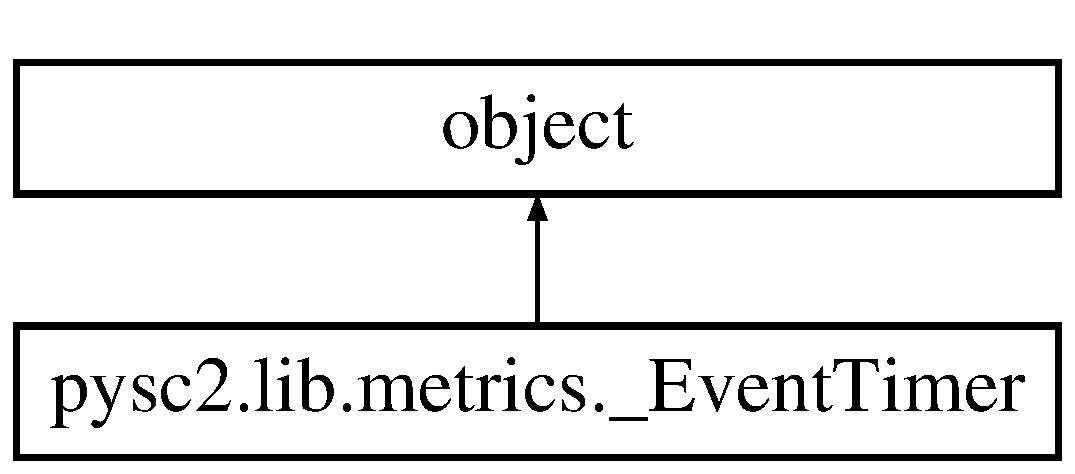
\includegraphics[height=2.000000cm]{classpysc2_1_1lib_1_1metrics_1_1___event_timer}
\end{center}
\end{figure}
\subsection*{Public Member Functions}
\begin{DoxyCompactItemize}
\item 
def \mbox{\hyperlink{classpysc2_1_1lib_1_1metrics_1_1___event_timer_a57a5b0557d7da12374767386bf2ba818}{\+\_\+\+\_\+enter\+\_\+\+\_\+}} (self)
\item 
def \mbox{\hyperlink{classpysc2_1_1lib_1_1metrics_1_1___event_timer_a41da3f624cce120628f8f6a2d1ec3a2c}{\+\_\+\+\_\+exit\+\_\+\+\_\+}} (self, unused\+\_\+exception\+\_\+type, unused\+\_\+exc\+\_\+value, unused\+\_\+traceback)
\end{DoxyCompactItemize}


\subsection{Detailed Description}
\begin{DoxyVerb}Example event timer to measure step and observation times.\end{DoxyVerb}
 

\subsection{Member Function Documentation}
\mbox{\Hypertarget{classpysc2_1_1lib_1_1metrics_1_1___event_timer_a57a5b0557d7da12374767386bf2ba818}\label{classpysc2_1_1lib_1_1metrics_1_1___event_timer_a57a5b0557d7da12374767386bf2ba818}} 
\index{pysc2\+::lib\+::metrics\+::\+\_\+\+Event\+Timer@{pysc2\+::lib\+::metrics\+::\+\_\+\+Event\+Timer}!\+\_\+\+\_\+enter\+\_\+\+\_\+@{\+\_\+\+\_\+enter\+\_\+\+\_\+}}
\index{\+\_\+\+\_\+enter\+\_\+\+\_\+@{\+\_\+\+\_\+enter\+\_\+\+\_\+}!pysc2\+::lib\+::metrics\+::\+\_\+\+Event\+Timer@{pysc2\+::lib\+::metrics\+::\+\_\+\+Event\+Timer}}
\subsubsection{\texorpdfstring{\+\_\+\+\_\+enter\+\_\+\+\_\+()}{\_\_enter\_\_()}}
{\footnotesize\ttfamily def pysc2.\+lib.\+metrics.\+\_\+\+Event\+Timer.\+\_\+\+\_\+enter\+\_\+\+\_\+ (\begin{DoxyParamCaption}\item[{}]{self }\end{DoxyParamCaption})}

\mbox{\Hypertarget{classpysc2_1_1lib_1_1metrics_1_1___event_timer_a41da3f624cce120628f8f6a2d1ec3a2c}\label{classpysc2_1_1lib_1_1metrics_1_1___event_timer_a41da3f624cce120628f8f6a2d1ec3a2c}} 
\index{pysc2\+::lib\+::metrics\+::\+\_\+\+Event\+Timer@{pysc2\+::lib\+::metrics\+::\+\_\+\+Event\+Timer}!\+\_\+\+\_\+exit\+\_\+\+\_\+@{\+\_\+\+\_\+exit\+\_\+\+\_\+}}
\index{\+\_\+\+\_\+exit\+\_\+\+\_\+@{\+\_\+\+\_\+exit\+\_\+\+\_\+}!pysc2\+::lib\+::metrics\+::\+\_\+\+Event\+Timer@{pysc2\+::lib\+::metrics\+::\+\_\+\+Event\+Timer}}
\subsubsection{\texorpdfstring{\+\_\+\+\_\+exit\+\_\+\+\_\+()}{\_\_exit\_\_()}}
{\footnotesize\ttfamily def pysc2.\+lib.\+metrics.\+\_\+\+Event\+Timer.\+\_\+\+\_\+exit\+\_\+\+\_\+ (\begin{DoxyParamCaption}\item[{}]{self,  }\item[{}]{unused\+\_\+exception\+\_\+type,  }\item[{}]{unused\+\_\+exc\+\_\+value,  }\item[{}]{unused\+\_\+traceback }\end{DoxyParamCaption})}



The documentation for this class was generated from the following file\+:\begin{DoxyCompactItemize}
\item 
lib/\mbox{\hyperlink{metrics_8py}{metrics.\+py}}\end{DoxyCompactItemize}

\hypertarget{classpysc2_1_1lib_1_1renderer__human_1_1___surface}{}\section{pysc2.\+lib.\+renderer\+\_\+human.\+\_\+\+Surface Class Reference}
\label{classpysc2_1_1lib_1_1renderer__human_1_1___surface}\index{pysc2.\+lib.\+renderer\+\_\+human.\+\_\+\+Surface@{pysc2.\+lib.\+renderer\+\_\+human.\+\_\+\+Surface}}
Inheritance diagram for pysc2.\+lib.\+renderer\+\_\+human.\+\_\+\+Surface\+:\begin{figure}[H]
\begin{center}
\leavevmode
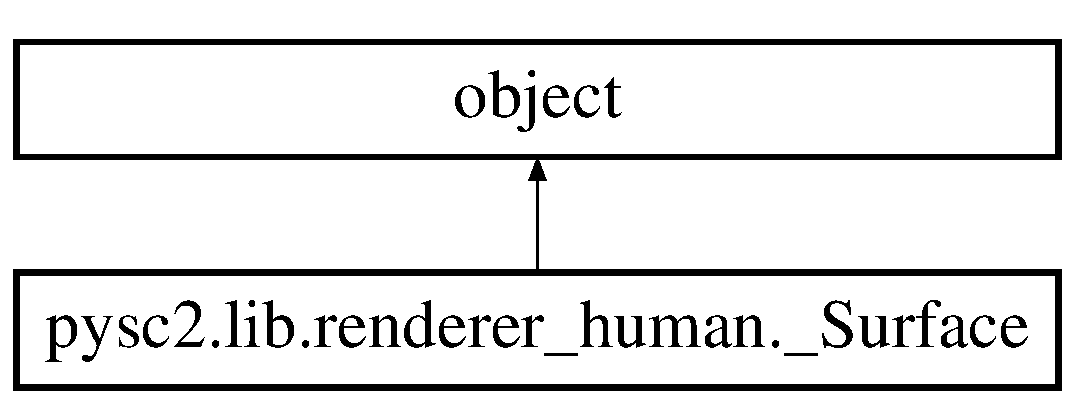
\includegraphics[height=2.000000cm]{classpysc2_1_1lib_1_1renderer__human_1_1___surface}
\end{center}
\end{figure}
\subsection*{Public Member Functions}
\begin{DoxyCompactItemize}
\item 
def \mbox{\hyperlink{classpysc2_1_1lib_1_1renderer__human_1_1___surface_a1357779bf7813158c9333300636fd107}{\+\_\+\+\_\+init\+\_\+\+\_\+}} (self, \mbox{\hyperlink{classpysc2_1_1lib_1_1renderer__human_1_1___surface_a4f0f39530a27df058f01c18e19f705f6}{surf}}, \mbox{\hyperlink{classpysc2_1_1lib_1_1renderer__human_1_1___surface_a5f951c622b86c80f949b09f274995ffe}{surf\+\_\+type}}, \mbox{\hyperlink{classpysc2_1_1lib_1_1renderer__human_1_1___surface_a3a7c29c8853fde7755b1c9908631a8b3}{surf\+\_\+rect}}, \mbox{\hyperlink{classpysc2_1_1lib_1_1renderer__human_1_1___surface_a76ded3196283f7e7104ba8f8a784c917}{world\+\_\+to\+\_\+surf}}, \mbox{\hyperlink{classpysc2_1_1lib_1_1renderer__human_1_1___surface_a7fa7b3c456fca16f552252649db7ac44}{world\+\_\+to\+\_\+obs}}, \mbox{\hyperlink{classpysc2_1_1lib_1_1renderer__human_1_1___surface_ada72ce60001e5107b602d6543007c9de}{draw}})
\item 
def \mbox{\hyperlink{classpysc2_1_1lib_1_1renderer__human_1_1___surface_a3147e67c55d537f3903e088ee03f7016}{draw\+\_\+arc}} (self, color, world\+\_\+loc, world\+\_\+radius, start\+\_\+angle, stop\+\_\+angle, thickness=1)
\item 
def \mbox{\hyperlink{classpysc2_1_1lib_1_1renderer__human_1_1___surface_a0dbda25a5a85520c8740e0d2a232848b}{draw\+\_\+circle}} (self, color, world\+\_\+loc, world\+\_\+radius, thickness=0)
\item 
def \mbox{\hyperlink{classpysc2_1_1lib_1_1renderer__human_1_1___surface_a8f798a0fa115c799ea7eeed7f0baa842}{draw\+\_\+rect}} (self, color, world\+\_\+rect, thickness=0)
\item 
def \mbox{\hyperlink{classpysc2_1_1lib_1_1renderer__human_1_1___surface_a586834302ec3b26934da8b2d5b3734f6}{blit\+\_\+np\+\_\+array}} (self, array)
\item 
def \mbox{\hyperlink{classpysc2_1_1lib_1_1renderer__human_1_1___surface_a2ff2cc7e501dfe9713ac4f7b56708a0c}{write\+\_\+screen}} (self, font, color, screen\+\_\+pos, text, align=\char`\"{}left\char`\"{}, valign=\char`\"{}top\char`\"{})
\end{DoxyCompactItemize}
\subsection*{Public Attributes}
\begin{DoxyCompactItemize}
\item 
\mbox{\hyperlink{classpysc2_1_1lib_1_1renderer__human_1_1___surface_a4f0f39530a27df058f01c18e19f705f6}{surf}}
\item 
\mbox{\hyperlink{classpysc2_1_1lib_1_1renderer__human_1_1___surface_a5f951c622b86c80f949b09f274995ffe}{surf\+\_\+type}}
\item 
\mbox{\hyperlink{classpysc2_1_1lib_1_1renderer__human_1_1___surface_a3a7c29c8853fde7755b1c9908631a8b3}{surf\+\_\+rect}}
\item 
\mbox{\hyperlink{classpysc2_1_1lib_1_1renderer__human_1_1___surface_a76ded3196283f7e7104ba8f8a784c917}{world\+\_\+to\+\_\+surf}}
\item 
\mbox{\hyperlink{classpysc2_1_1lib_1_1renderer__human_1_1___surface_a7fa7b3c456fca16f552252649db7ac44}{world\+\_\+to\+\_\+obs}}
\item 
\mbox{\hyperlink{classpysc2_1_1lib_1_1renderer__human_1_1___surface_ada72ce60001e5107b602d6543007c9de}{draw}}
\end{DoxyCompactItemize}


\subsection{Detailed Description}
\begin{DoxyVerb}A surface to display on screen.\end{DoxyVerb}
 

\subsection{Constructor \& Destructor Documentation}
\mbox{\Hypertarget{classpysc2_1_1lib_1_1renderer__human_1_1___surface_a1357779bf7813158c9333300636fd107}\label{classpysc2_1_1lib_1_1renderer__human_1_1___surface_a1357779bf7813158c9333300636fd107}} 
\index{pysc2\+::lib\+::renderer\+\_\+human\+::\+\_\+\+Surface@{pysc2\+::lib\+::renderer\+\_\+human\+::\+\_\+\+Surface}!\+\_\+\+\_\+init\+\_\+\+\_\+@{\+\_\+\+\_\+init\+\_\+\+\_\+}}
\index{\+\_\+\+\_\+init\+\_\+\+\_\+@{\+\_\+\+\_\+init\+\_\+\+\_\+}!pysc2\+::lib\+::renderer\+\_\+human\+::\+\_\+\+Surface@{pysc2\+::lib\+::renderer\+\_\+human\+::\+\_\+\+Surface}}
\subsubsection{\texorpdfstring{\+\_\+\+\_\+init\+\_\+\+\_\+()}{\_\_init\_\_()}}
{\footnotesize\ttfamily def pysc2.\+lib.\+renderer\+\_\+human.\+\_\+\+Surface.\+\_\+\+\_\+init\+\_\+\+\_\+ (\begin{DoxyParamCaption}\item[{}]{self,  }\item[{}]{surf,  }\item[{}]{surf\+\_\+type,  }\item[{}]{surf\+\_\+rect,  }\item[{}]{world\+\_\+to\+\_\+surf,  }\item[{}]{world\+\_\+to\+\_\+obs,  }\item[{}]{draw }\end{DoxyParamCaption})}

\begin{DoxyVerb}A surface to display on screen.

Args:
  surf: The actual pygame.Surface (or subsurface).
  surf_type: A SurfType, used to tell how to treat clicks in that area.
  surf_rect: Rect of the surface relative to the window.
  world_to_surf: Convert a world point to a pixel on the surface.
  world_to_obs: Convert a world point to a pixel in the observation.
  draw: A function that draws onto the surface.
\end{DoxyVerb}
 

\subsection{Member Function Documentation}
\mbox{\Hypertarget{classpysc2_1_1lib_1_1renderer__human_1_1___surface_a586834302ec3b26934da8b2d5b3734f6}\label{classpysc2_1_1lib_1_1renderer__human_1_1___surface_a586834302ec3b26934da8b2d5b3734f6}} 
\index{pysc2\+::lib\+::renderer\+\_\+human\+::\+\_\+\+Surface@{pysc2\+::lib\+::renderer\+\_\+human\+::\+\_\+\+Surface}!blit\+\_\+np\+\_\+array@{blit\+\_\+np\+\_\+array}}
\index{blit\+\_\+np\+\_\+array@{blit\+\_\+np\+\_\+array}!pysc2\+::lib\+::renderer\+\_\+human\+::\+\_\+\+Surface@{pysc2\+::lib\+::renderer\+\_\+human\+::\+\_\+\+Surface}}
\subsubsection{\texorpdfstring{blit\+\_\+np\+\_\+array()}{blit\_np\_array()}}
{\footnotesize\ttfamily def pysc2.\+lib.\+renderer\+\_\+human.\+\_\+\+Surface.\+blit\+\_\+np\+\_\+array (\begin{DoxyParamCaption}\item[{}]{self,  }\item[{}]{array }\end{DoxyParamCaption})}

\begin{DoxyVerb}Fill this surface using the contents of a numpy array.\end{DoxyVerb}
 \mbox{\Hypertarget{classpysc2_1_1lib_1_1renderer__human_1_1___surface_a3147e67c55d537f3903e088ee03f7016}\label{classpysc2_1_1lib_1_1renderer__human_1_1___surface_a3147e67c55d537f3903e088ee03f7016}} 
\index{pysc2\+::lib\+::renderer\+\_\+human\+::\+\_\+\+Surface@{pysc2\+::lib\+::renderer\+\_\+human\+::\+\_\+\+Surface}!draw\+\_\+arc@{draw\+\_\+arc}}
\index{draw\+\_\+arc@{draw\+\_\+arc}!pysc2\+::lib\+::renderer\+\_\+human\+::\+\_\+\+Surface@{pysc2\+::lib\+::renderer\+\_\+human\+::\+\_\+\+Surface}}
\subsubsection{\texorpdfstring{draw\+\_\+arc()}{draw\_arc()}}
{\footnotesize\ttfamily def pysc2.\+lib.\+renderer\+\_\+human.\+\_\+\+Surface.\+draw\+\_\+arc (\begin{DoxyParamCaption}\item[{}]{self,  }\item[{}]{color,  }\item[{}]{world\+\_\+loc,  }\item[{}]{world\+\_\+radius,  }\item[{}]{start\+\_\+angle,  }\item[{}]{stop\+\_\+angle,  }\item[{}]{thickness = {\ttfamily 1} }\end{DoxyParamCaption})}

\begin{DoxyVerb}Draw an arc using world coordinates, radius, start and stop angles.\end{DoxyVerb}
 \mbox{\Hypertarget{classpysc2_1_1lib_1_1renderer__human_1_1___surface_a0dbda25a5a85520c8740e0d2a232848b}\label{classpysc2_1_1lib_1_1renderer__human_1_1___surface_a0dbda25a5a85520c8740e0d2a232848b}} 
\index{pysc2\+::lib\+::renderer\+\_\+human\+::\+\_\+\+Surface@{pysc2\+::lib\+::renderer\+\_\+human\+::\+\_\+\+Surface}!draw\+\_\+circle@{draw\+\_\+circle}}
\index{draw\+\_\+circle@{draw\+\_\+circle}!pysc2\+::lib\+::renderer\+\_\+human\+::\+\_\+\+Surface@{pysc2\+::lib\+::renderer\+\_\+human\+::\+\_\+\+Surface}}
\subsubsection{\texorpdfstring{draw\+\_\+circle()}{draw\_circle()}}
{\footnotesize\ttfamily def pysc2.\+lib.\+renderer\+\_\+human.\+\_\+\+Surface.\+draw\+\_\+circle (\begin{DoxyParamCaption}\item[{}]{self,  }\item[{}]{color,  }\item[{}]{world\+\_\+loc,  }\item[{}]{world\+\_\+radius,  }\item[{}]{thickness = {\ttfamily 0} }\end{DoxyParamCaption})}

\begin{DoxyVerb}Draw a circle using world coordinates and radius.\end{DoxyVerb}
 \mbox{\Hypertarget{classpysc2_1_1lib_1_1renderer__human_1_1___surface_a8f798a0fa115c799ea7eeed7f0baa842}\label{classpysc2_1_1lib_1_1renderer__human_1_1___surface_a8f798a0fa115c799ea7eeed7f0baa842}} 
\index{pysc2\+::lib\+::renderer\+\_\+human\+::\+\_\+\+Surface@{pysc2\+::lib\+::renderer\+\_\+human\+::\+\_\+\+Surface}!draw\+\_\+rect@{draw\+\_\+rect}}
\index{draw\+\_\+rect@{draw\+\_\+rect}!pysc2\+::lib\+::renderer\+\_\+human\+::\+\_\+\+Surface@{pysc2\+::lib\+::renderer\+\_\+human\+::\+\_\+\+Surface}}
\subsubsection{\texorpdfstring{draw\+\_\+rect()}{draw\_rect()}}
{\footnotesize\ttfamily def pysc2.\+lib.\+renderer\+\_\+human.\+\_\+\+Surface.\+draw\+\_\+rect (\begin{DoxyParamCaption}\item[{}]{self,  }\item[{}]{color,  }\item[{}]{world\+\_\+rect,  }\item[{}]{thickness = {\ttfamily 0} }\end{DoxyParamCaption})}

\begin{DoxyVerb}Draw a rectangle using world coordinates.\end{DoxyVerb}
 \mbox{\Hypertarget{classpysc2_1_1lib_1_1renderer__human_1_1___surface_a2ff2cc7e501dfe9713ac4f7b56708a0c}\label{classpysc2_1_1lib_1_1renderer__human_1_1___surface_a2ff2cc7e501dfe9713ac4f7b56708a0c}} 
\index{pysc2\+::lib\+::renderer\+\_\+human\+::\+\_\+\+Surface@{pysc2\+::lib\+::renderer\+\_\+human\+::\+\_\+\+Surface}!write\+\_\+screen@{write\+\_\+screen}}
\index{write\+\_\+screen@{write\+\_\+screen}!pysc2\+::lib\+::renderer\+\_\+human\+::\+\_\+\+Surface@{pysc2\+::lib\+::renderer\+\_\+human\+::\+\_\+\+Surface}}
\subsubsection{\texorpdfstring{write\+\_\+screen()}{write\_screen()}}
{\footnotesize\ttfamily def pysc2.\+lib.\+renderer\+\_\+human.\+\_\+\+Surface.\+write\+\_\+screen (\begin{DoxyParamCaption}\item[{}]{self,  }\item[{}]{font,  }\item[{}]{color,  }\item[{}]{screen\+\_\+pos,  }\item[{}]{text,  }\item[{}]{align = {\ttfamily \char`\"{}left\char`\"{}},  }\item[{}]{valign = {\ttfamily \char`\"{}top\char`\"{}} }\end{DoxyParamCaption})}

\begin{DoxyVerb}Write to the screen in font.size relative coordinates.\end{DoxyVerb}
 

\subsection{Member Data Documentation}
\mbox{\Hypertarget{classpysc2_1_1lib_1_1renderer__human_1_1___surface_ada72ce60001e5107b602d6543007c9de}\label{classpysc2_1_1lib_1_1renderer__human_1_1___surface_ada72ce60001e5107b602d6543007c9de}} 
\index{pysc2\+::lib\+::renderer\+\_\+human\+::\+\_\+\+Surface@{pysc2\+::lib\+::renderer\+\_\+human\+::\+\_\+\+Surface}!draw@{draw}}
\index{draw@{draw}!pysc2\+::lib\+::renderer\+\_\+human\+::\+\_\+\+Surface@{pysc2\+::lib\+::renderer\+\_\+human\+::\+\_\+\+Surface}}
\subsubsection{\texorpdfstring{draw}{draw}}
{\footnotesize\ttfamily pysc2.\+lib.\+renderer\+\_\+human.\+\_\+\+Surface.\+draw}

\mbox{\Hypertarget{classpysc2_1_1lib_1_1renderer__human_1_1___surface_a4f0f39530a27df058f01c18e19f705f6}\label{classpysc2_1_1lib_1_1renderer__human_1_1___surface_a4f0f39530a27df058f01c18e19f705f6}} 
\index{pysc2\+::lib\+::renderer\+\_\+human\+::\+\_\+\+Surface@{pysc2\+::lib\+::renderer\+\_\+human\+::\+\_\+\+Surface}!surf@{surf}}
\index{surf@{surf}!pysc2\+::lib\+::renderer\+\_\+human\+::\+\_\+\+Surface@{pysc2\+::lib\+::renderer\+\_\+human\+::\+\_\+\+Surface}}
\subsubsection{\texorpdfstring{surf}{surf}}
{\footnotesize\ttfamily pysc2.\+lib.\+renderer\+\_\+human.\+\_\+\+Surface.\+surf}

\mbox{\Hypertarget{classpysc2_1_1lib_1_1renderer__human_1_1___surface_a3a7c29c8853fde7755b1c9908631a8b3}\label{classpysc2_1_1lib_1_1renderer__human_1_1___surface_a3a7c29c8853fde7755b1c9908631a8b3}} 
\index{pysc2\+::lib\+::renderer\+\_\+human\+::\+\_\+\+Surface@{pysc2\+::lib\+::renderer\+\_\+human\+::\+\_\+\+Surface}!surf\+\_\+rect@{surf\+\_\+rect}}
\index{surf\+\_\+rect@{surf\+\_\+rect}!pysc2\+::lib\+::renderer\+\_\+human\+::\+\_\+\+Surface@{pysc2\+::lib\+::renderer\+\_\+human\+::\+\_\+\+Surface}}
\subsubsection{\texorpdfstring{surf\+\_\+rect}{surf\_rect}}
{\footnotesize\ttfamily pysc2.\+lib.\+renderer\+\_\+human.\+\_\+\+Surface.\+surf\+\_\+rect}

\mbox{\Hypertarget{classpysc2_1_1lib_1_1renderer__human_1_1___surface_a5f951c622b86c80f949b09f274995ffe}\label{classpysc2_1_1lib_1_1renderer__human_1_1___surface_a5f951c622b86c80f949b09f274995ffe}} 
\index{pysc2\+::lib\+::renderer\+\_\+human\+::\+\_\+\+Surface@{pysc2\+::lib\+::renderer\+\_\+human\+::\+\_\+\+Surface}!surf\+\_\+type@{surf\+\_\+type}}
\index{surf\+\_\+type@{surf\+\_\+type}!pysc2\+::lib\+::renderer\+\_\+human\+::\+\_\+\+Surface@{pysc2\+::lib\+::renderer\+\_\+human\+::\+\_\+\+Surface}}
\subsubsection{\texorpdfstring{surf\+\_\+type}{surf\_type}}
{\footnotesize\ttfamily pysc2.\+lib.\+renderer\+\_\+human.\+\_\+\+Surface.\+surf\+\_\+type}

\mbox{\Hypertarget{classpysc2_1_1lib_1_1renderer__human_1_1___surface_a7fa7b3c456fca16f552252649db7ac44}\label{classpysc2_1_1lib_1_1renderer__human_1_1___surface_a7fa7b3c456fca16f552252649db7ac44}} 
\index{pysc2\+::lib\+::renderer\+\_\+human\+::\+\_\+\+Surface@{pysc2\+::lib\+::renderer\+\_\+human\+::\+\_\+\+Surface}!world\+\_\+to\+\_\+obs@{world\+\_\+to\+\_\+obs}}
\index{world\+\_\+to\+\_\+obs@{world\+\_\+to\+\_\+obs}!pysc2\+::lib\+::renderer\+\_\+human\+::\+\_\+\+Surface@{pysc2\+::lib\+::renderer\+\_\+human\+::\+\_\+\+Surface}}
\subsubsection{\texorpdfstring{world\+\_\+to\+\_\+obs}{world\_to\_obs}}
{\footnotesize\ttfamily pysc2.\+lib.\+renderer\+\_\+human.\+\_\+\+Surface.\+world\+\_\+to\+\_\+obs}

\mbox{\Hypertarget{classpysc2_1_1lib_1_1renderer__human_1_1___surface_a76ded3196283f7e7104ba8f8a784c917}\label{classpysc2_1_1lib_1_1renderer__human_1_1___surface_a76ded3196283f7e7104ba8f8a784c917}} 
\index{pysc2\+::lib\+::renderer\+\_\+human\+::\+\_\+\+Surface@{pysc2\+::lib\+::renderer\+\_\+human\+::\+\_\+\+Surface}!world\+\_\+to\+\_\+surf@{world\+\_\+to\+\_\+surf}}
\index{world\+\_\+to\+\_\+surf@{world\+\_\+to\+\_\+surf}!pysc2\+::lib\+::renderer\+\_\+human\+::\+\_\+\+Surface@{pysc2\+::lib\+::renderer\+\_\+human\+::\+\_\+\+Surface}}
\subsubsection{\texorpdfstring{world\+\_\+to\+\_\+surf}{world\_to\_surf}}
{\footnotesize\ttfamily pysc2.\+lib.\+renderer\+\_\+human.\+\_\+\+Surface.\+world\+\_\+to\+\_\+surf}



The documentation for this class was generated from the following file\+:\begin{DoxyCompactItemize}
\item 
lib/\mbox{\hyperlink{renderer__human_8py}{renderer\+\_\+human.\+py}}\end{DoxyCompactItemize}

\hypertarget{classpysc2_1_1env_1_1mock__sc2__env_1_1___test_environment}{}\section{pysc2.\+env.\+mock\+\_\+sc2\+\_\+env.\+\_\+\+Test\+Environment Class Reference}
\label{classpysc2_1_1env_1_1mock__sc2__env_1_1___test_environment}\index{pysc2.\+env.\+mock\+\_\+sc2\+\_\+env.\+\_\+\+Test\+Environment@{pysc2.\+env.\+mock\+\_\+sc2\+\_\+env.\+\_\+\+Test\+Environment}}
Inheritance diagram for pysc2.\+env.\+mock\+\_\+sc2\+\_\+env.\+\_\+\+Test\+Environment\+:\begin{figure}[H]
\begin{center}
\leavevmode
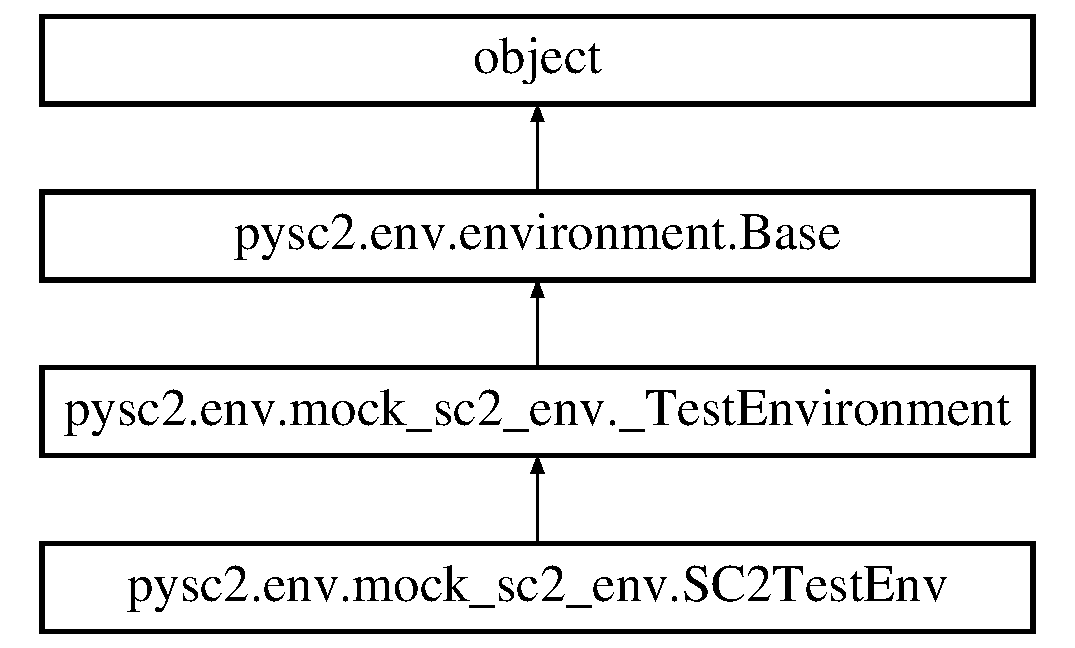
\includegraphics[height=4.000000cm]{classpysc2_1_1env_1_1mock__sc2__env_1_1___test_environment}
\end{center}
\end{figure}
\subsection*{Public Member Functions}
\begin{DoxyCompactItemize}
\item 
def \mbox{\hyperlink{classpysc2_1_1env_1_1mock__sc2__env_1_1___test_environment_ad3acb8d357a313a916e134895503f4bd}{\+\_\+\+\_\+init\+\_\+\+\_\+}} (self, num\+\_\+agents, \mbox{\hyperlink{classpysc2_1_1env_1_1mock__sc2__env_1_1___test_environment_a231da0c879e81efdb7a929be37f22311}{observation\+\_\+spec}}, \mbox{\hyperlink{classpysc2_1_1env_1_1mock__sc2__env_1_1___test_environment_ae7ce75b41709291c06f255bf682172bb}{action\+\_\+spec}})
\item 
def \mbox{\hyperlink{classpysc2_1_1env_1_1mock__sc2__env_1_1___test_environment_a995a511044613e7d5f4452a6238cd3eb}{reset}} (self)
\item 
def \mbox{\hyperlink{classpysc2_1_1env_1_1mock__sc2__env_1_1___test_environment_affd351d46e26ada4c242072c08418ae1}{step}} (self, actions)
\item 
def \mbox{\hyperlink{classpysc2_1_1env_1_1mock__sc2__env_1_1___test_environment_ae7ce75b41709291c06f255bf682172bb}{action\+\_\+spec}} (self)
\item 
def \mbox{\hyperlink{classpysc2_1_1env_1_1mock__sc2__env_1_1___test_environment_a231da0c879e81efdb7a929be37f22311}{observation\+\_\+spec}} (self)
\end{DoxyCompactItemize}
\subsection*{Public Attributes}
\begin{DoxyCompactItemize}
\item 
\mbox{\hyperlink{classpysc2_1_1env_1_1mock__sc2__env_1_1___test_environment_ae8d2e3dc5088a409252d626f2d35203d}{next\+\_\+timestep}}
\item 
\mbox{\hyperlink{classpysc2_1_1env_1_1mock__sc2__env_1_1___test_environment_a2c0bd6e676d1490b3b528831ca501534}{episode\+\_\+length}}
\end{DoxyCompactItemize}


\subsection{Detailed Description}
\begin{DoxyVerb}A simple generic test environment.

This class is a lightweight implementation of `environment.Base` that returns
the same timesteps on every observation call. By default, each returned
timestep (one per agent) is reward 0., discount 1., and the observations are
zero `np.ndarrays` of dtype `np.int32` and the shape specified by the
environment's spec.

However, the behavior of the `TestEnvironment` can be configured using the
object's attributes.

Attributes:
  next_timestep: The `environment.TimeStep`s to return on the next call to
    `step`. When necessary, some fields will be overridden to ensure the
    `step_type` contract.
  episode_length: if the episode length (number of transitions) exceeds
    `episode_length` on a call to `step`, the `step-type` will be set to
    `environment.StepType.LAST`, forcing an end of episode. This allows a
    stub of a production environment to have end_episodes. Will be ignored if
    set to `float('inf')` (the default).
\end{DoxyVerb}
 

\subsection{Constructor \& Destructor Documentation}
\mbox{\Hypertarget{classpysc2_1_1env_1_1mock__sc2__env_1_1___test_environment_ad3acb8d357a313a916e134895503f4bd}\label{classpysc2_1_1env_1_1mock__sc2__env_1_1___test_environment_ad3acb8d357a313a916e134895503f4bd}} 
\index{pysc2\+::env\+::mock\+\_\+sc2\+\_\+env\+::\+\_\+\+Test\+Environment@{pysc2\+::env\+::mock\+\_\+sc2\+\_\+env\+::\+\_\+\+Test\+Environment}!\+\_\+\+\_\+init\+\_\+\+\_\+@{\+\_\+\+\_\+init\+\_\+\+\_\+}}
\index{\+\_\+\+\_\+init\+\_\+\+\_\+@{\+\_\+\+\_\+init\+\_\+\+\_\+}!pysc2\+::env\+::mock\+\_\+sc2\+\_\+env\+::\+\_\+\+Test\+Environment@{pysc2\+::env\+::mock\+\_\+sc2\+\_\+env\+::\+\_\+\+Test\+Environment}}
\subsubsection{\texorpdfstring{\+\_\+\+\_\+init\+\_\+\+\_\+()}{\_\_init\_\_()}}
{\footnotesize\ttfamily def pysc2.\+env.\+mock\+\_\+sc2\+\_\+env.\+\_\+\+Test\+Environment.\+\_\+\+\_\+init\+\_\+\+\_\+ (\begin{DoxyParamCaption}\item[{}]{self,  }\item[{}]{num\+\_\+agents,  }\item[{}]{observation\+\_\+spec,  }\item[{}]{action\+\_\+spec }\end{DoxyParamCaption})}

\begin{DoxyVerb}Initializes the TestEnvironment.

The `next_observation` is initialized to be reward = 0., discount = 1.,
and an appropriately sized observation of all zeros. `episode_length` is set
to `float('inf')`.

Args:
  num_agents: The number of agents.
  observation_spec: The observation specs for each player.
  action_spec: The action specs for each player.
\end{DoxyVerb}
 

\subsection{Member Function Documentation}
\mbox{\Hypertarget{classpysc2_1_1env_1_1mock__sc2__env_1_1___test_environment_ae7ce75b41709291c06f255bf682172bb}\label{classpysc2_1_1env_1_1mock__sc2__env_1_1___test_environment_ae7ce75b41709291c06f255bf682172bb}} 
\index{pysc2\+::env\+::mock\+\_\+sc2\+\_\+env\+::\+\_\+\+Test\+Environment@{pysc2\+::env\+::mock\+\_\+sc2\+\_\+env\+::\+\_\+\+Test\+Environment}!action\+\_\+spec@{action\+\_\+spec}}
\index{action\+\_\+spec@{action\+\_\+spec}!pysc2\+::env\+::mock\+\_\+sc2\+\_\+env\+::\+\_\+\+Test\+Environment@{pysc2\+::env\+::mock\+\_\+sc2\+\_\+env\+::\+\_\+\+Test\+Environment}}
\subsubsection{\texorpdfstring{action\+\_\+spec()}{action\_spec()}}
{\footnotesize\ttfamily def pysc2.\+env.\+mock\+\_\+sc2\+\_\+env.\+\_\+\+Test\+Environment.\+action\+\_\+spec (\begin{DoxyParamCaption}\item[{}]{self }\end{DoxyParamCaption})}

\begin{DoxyVerb}See base class.\end{DoxyVerb}
 \mbox{\Hypertarget{classpysc2_1_1env_1_1mock__sc2__env_1_1___test_environment_a231da0c879e81efdb7a929be37f22311}\label{classpysc2_1_1env_1_1mock__sc2__env_1_1___test_environment_a231da0c879e81efdb7a929be37f22311}} 
\index{pysc2\+::env\+::mock\+\_\+sc2\+\_\+env\+::\+\_\+\+Test\+Environment@{pysc2\+::env\+::mock\+\_\+sc2\+\_\+env\+::\+\_\+\+Test\+Environment}!observation\+\_\+spec@{observation\+\_\+spec}}
\index{observation\+\_\+spec@{observation\+\_\+spec}!pysc2\+::env\+::mock\+\_\+sc2\+\_\+env\+::\+\_\+\+Test\+Environment@{pysc2\+::env\+::mock\+\_\+sc2\+\_\+env\+::\+\_\+\+Test\+Environment}}
\subsubsection{\texorpdfstring{observation\+\_\+spec()}{observation\_spec()}}
{\footnotesize\ttfamily def pysc2.\+env.\+mock\+\_\+sc2\+\_\+env.\+\_\+\+Test\+Environment.\+observation\+\_\+spec (\begin{DoxyParamCaption}\item[{}]{self }\end{DoxyParamCaption})}

\begin{DoxyVerb}See base class.\end{DoxyVerb}
 \mbox{\Hypertarget{classpysc2_1_1env_1_1mock__sc2__env_1_1___test_environment_a995a511044613e7d5f4452a6238cd3eb}\label{classpysc2_1_1env_1_1mock__sc2__env_1_1___test_environment_a995a511044613e7d5f4452a6238cd3eb}} 
\index{pysc2\+::env\+::mock\+\_\+sc2\+\_\+env\+::\+\_\+\+Test\+Environment@{pysc2\+::env\+::mock\+\_\+sc2\+\_\+env\+::\+\_\+\+Test\+Environment}!reset@{reset}}
\index{reset@{reset}!pysc2\+::env\+::mock\+\_\+sc2\+\_\+env\+::\+\_\+\+Test\+Environment@{pysc2\+::env\+::mock\+\_\+sc2\+\_\+env\+::\+\_\+\+Test\+Environment}}
\subsubsection{\texorpdfstring{reset()}{reset()}}
{\footnotesize\ttfamily def pysc2.\+env.\+mock\+\_\+sc2\+\_\+env.\+\_\+\+Test\+Environment.\+reset (\begin{DoxyParamCaption}\item[{}]{self }\end{DoxyParamCaption})}

\begin{DoxyVerb}Restarts episode and returns `next_observation` with `StepType.FIRST`.\end{DoxyVerb}
 \mbox{\Hypertarget{classpysc2_1_1env_1_1mock__sc2__env_1_1___test_environment_affd351d46e26ada4c242072c08418ae1}\label{classpysc2_1_1env_1_1mock__sc2__env_1_1___test_environment_affd351d46e26ada4c242072c08418ae1}} 
\index{pysc2\+::env\+::mock\+\_\+sc2\+\_\+env\+::\+\_\+\+Test\+Environment@{pysc2\+::env\+::mock\+\_\+sc2\+\_\+env\+::\+\_\+\+Test\+Environment}!step@{step}}
\index{step@{step}!pysc2\+::env\+::mock\+\_\+sc2\+\_\+env\+::\+\_\+\+Test\+Environment@{pysc2\+::env\+::mock\+\_\+sc2\+\_\+env\+::\+\_\+\+Test\+Environment}}
\subsubsection{\texorpdfstring{step()}{step()}}
{\footnotesize\ttfamily def pysc2.\+env.\+mock\+\_\+sc2\+\_\+env.\+\_\+\+Test\+Environment.\+step (\begin{DoxyParamCaption}\item[{}]{self,  }\item[{}]{actions }\end{DoxyParamCaption})}

\begin{DoxyVerb}Returns `next_observation` modifying its `step_type` if necessary.\end{DoxyVerb}
 

\subsection{Member Data Documentation}
\mbox{\Hypertarget{classpysc2_1_1env_1_1mock__sc2__env_1_1___test_environment_a2c0bd6e676d1490b3b528831ca501534}\label{classpysc2_1_1env_1_1mock__sc2__env_1_1___test_environment_a2c0bd6e676d1490b3b528831ca501534}} 
\index{pysc2\+::env\+::mock\+\_\+sc2\+\_\+env\+::\+\_\+\+Test\+Environment@{pysc2\+::env\+::mock\+\_\+sc2\+\_\+env\+::\+\_\+\+Test\+Environment}!episode\+\_\+length@{episode\+\_\+length}}
\index{episode\+\_\+length@{episode\+\_\+length}!pysc2\+::env\+::mock\+\_\+sc2\+\_\+env\+::\+\_\+\+Test\+Environment@{pysc2\+::env\+::mock\+\_\+sc2\+\_\+env\+::\+\_\+\+Test\+Environment}}
\subsubsection{\texorpdfstring{episode\+\_\+length}{episode\_length}}
{\footnotesize\ttfamily pysc2.\+env.\+mock\+\_\+sc2\+\_\+env.\+\_\+\+Test\+Environment.\+episode\+\_\+length}

\mbox{\Hypertarget{classpysc2_1_1env_1_1mock__sc2__env_1_1___test_environment_ae8d2e3dc5088a409252d626f2d35203d}\label{classpysc2_1_1env_1_1mock__sc2__env_1_1___test_environment_ae8d2e3dc5088a409252d626f2d35203d}} 
\index{pysc2\+::env\+::mock\+\_\+sc2\+\_\+env\+::\+\_\+\+Test\+Environment@{pysc2\+::env\+::mock\+\_\+sc2\+\_\+env\+::\+\_\+\+Test\+Environment}!next\+\_\+timestep@{next\+\_\+timestep}}
\index{next\+\_\+timestep@{next\+\_\+timestep}!pysc2\+::env\+::mock\+\_\+sc2\+\_\+env\+::\+\_\+\+Test\+Environment@{pysc2\+::env\+::mock\+\_\+sc2\+\_\+env\+::\+\_\+\+Test\+Environment}}
\subsubsection{\texorpdfstring{next\+\_\+timestep}{next\_timestep}}
{\footnotesize\ttfamily pysc2.\+env.\+mock\+\_\+sc2\+\_\+env.\+\_\+\+Test\+Environment.\+next\+\_\+timestep}



The documentation for this class was generated from the following file\+:\begin{DoxyCompactItemize}
\item 
env/\mbox{\hyperlink{mock__sc2__env_8py}{mock\+\_\+sc2\+\_\+env.\+py}}\end{DoxyCompactItemize}

\hypertarget{classpysc2_1_1env_1_1mock__sc2__env__test_1_1___test_mixin}{}\section{pysc2.\+env.\+mock\+\_\+sc2\+\_\+env\+\_\+test.\+\_\+\+Test\+Mixin Class Reference}
\label{classpysc2_1_1env_1_1mock__sc2__env__test_1_1___test_mixin}\index{pysc2.\+env.\+mock\+\_\+sc2\+\_\+env\+\_\+test.\+\_\+\+Test\+Mixin@{pysc2.\+env.\+mock\+\_\+sc2\+\_\+env\+\_\+test.\+\_\+\+Test\+Mixin}}
Inheritance diagram for pysc2.\+env.\+mock\+\_\+sc2\+\_\+env\+\_\+test.\+\_\+\+Test\+Mixin\+:\begin{figure}[H]
\begin{center}
\leavevmode
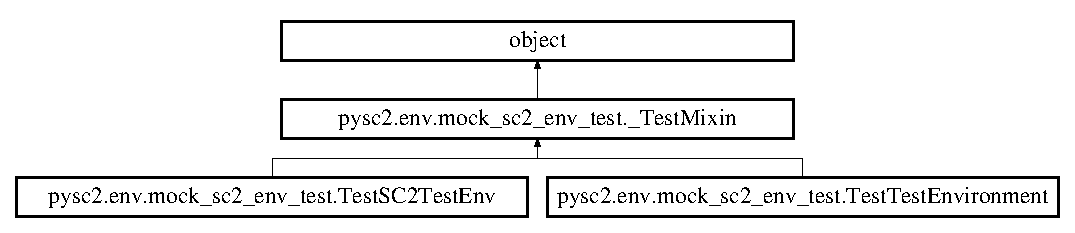
\includegraphics[height=2.683706cm]{classpysc2_1_1env_1_1mock__sc2__env__test_1_1___test_mixin}
\end{center}
\end{figure}
\subsection*{Public Member Functions}
\begin{DoxyCompactItemize}
\item 
def \mbox{\hyperlink{classpysc2_1_1env_1_1mock__sc2__env__test_1_1___test_mixin_ae44862283422b3f9f4cff0364e7718fe}{assert\+\_\+spec}} (self, array, shape, dtype)
\item 
def \mbox{\hyperlink{classpysc2_1_1env_1_1mock__sc2__env__test_1_1___test_mixin_adadfb2c15fcb2d44285adfe0abdda38b}{assert\+\_\+equal}} (self, actual, expected)
\item 
def \mbox{\hyperlink{classpysc2_1_1env_1_1mock__sc2__env__test_1_1___test_mixin_ae9e82d6e4019a1f2c3101bebbb570988}{assert\+\_\+reset}} (self, env)
\item 
def \mbox{\hyperlink{classpysc2_1_1env_1_1mock__sc2__env__test_1_1___test_mixin_a4c77f1899a786872425080daa843b2c4}{assert\+\_\+first\+\_\+step}} (self, env)
\item 
def \mbox{\hyperlink{classpysc2_1_1env_1_1mock__sc2__env__test_1_1___test_mixin_ae0bece3faa1dfe55f8a9057fe33e6522}{assert\+\_\+mid\+\_\+step}} (self, env)
\item 
def \mbox{\hyperlink{classpysc2_1_1env_1_1mock__sc2__env__test_1_1___test_mixin_a52dcd33d92eb8498d7986def1cb48626}{assert\+\_\+last\+\_\+step}} (self, env)
\end{DoxyCompactItemize}


\subsection{Member Function Documentation}
\mbox{\Hypertarget{classpysc2_1_1env_1_1mock__sc2__env__test_1_1___test_mixin_adadfb2c15fcb2d44285adfe0abdda38b}\label{classpysc2_1_1env_1_1mock__sc2__env__test_1_1___test_mixin_adadfb2c15fcb2d44285adfe0abdda38b}} 
\index{pysc2\+::env\+::mock\+\_\+sc2\+\_\+env\+\_\+test\+::\+\_\+\+Test\+Mixin@{pysc2\+::env\+::mock\+\_\+sc2\+\_\+env\+\_\+test\+::\+\_\+\+Test\+Mixin}!assert\+\_\+equal@{assert\+\_\+equal}}
\index{assert\+\_\+equal@{assert\+\_\+equal}!pysc2\+::env\+::mock\+\_\+sc2\+\_\+env\+\_\+test\+::\+\_\+\+Test\+Mixin@{pysc2\+::env\+::mock\+\_\+sc2\+\_\+env\+\_\+test\+::\+\_\+\+Test\+Mixin}}
\subsubsection{\texorpdfstring{assert\+\_\+equal()}{assert\_equal()}}
{\footnotesize\ttfamily def pysc2.\+env.\+mock\+\_\+sc2\+\_\+env\+\_\+test.\+\_\+\+Test\+Mixin.\+assert\+\_\+equal (\begin{DoxyParamCaption}\item[{}]{self,  }\item[{}]{actual,  }\item[{}]{expected }\end{DoxyParamCaption})}

\mbox{\Hypertarget{classpysc2_1_1env_1_1mock__sc2__env__test_1_1___test_mixin_a4c77f1899a786872425080daa843b2c4}\label{classpysc2_1_1env_1_1mock__sc2__env__test_1_1___test_mixin_a4c77f1899a786872425080daa843b2c4}} 
\index{pysc2\+::env\+::mock\+\_\+sc2\+\_\+env\+\_\+test\+::\+\_\+\+Test\+Mixin@{pysc2\+::env\+::mock\+\_\+sc2\+\_\+env\+\_\+test\+::\+\_\+\+Test\+Mixin}!assert\+\_\+first\+\_\+step@{assert\+\_\+first\+\_\+step}}
\index{assert\+\_\+first\+\_\+step@{assert\+\_\+first\+\_\+step}!pysc2\+::env\+::mock\+\_\+sc2\+\_\+env\+\_\+test\+::\+\_\+\+Test\+Mixin@{pysc2\+::env\+::mock\+\_\+sc2\+\_\+env\+\_\+test\+::\+\_\+\+Test\+Mixin}}
\subsubsection{\texorpdfstring{assert\+\_\+first\+\_\+step()}{assert\_first\_step()}}
{\footnotesize\ttfamily def pysc2.\+env.\+mock\+\_\+sc2\+\_\+env\+\_\+test.\+\_\+\+Test\+Mixin.\+assert\+\_\+first\+\_\+step (\begin{DoxyParamCaption}\item[{}]{self,  }\item[{}]{env }\end{DoxyParamCaption})}

\mbox{\Hypertarget{classpysc2_1_1env_1_1mock__sc2__env__test_1_1___test_mixin_a52dcd33d92eb8498d7986def1cb48626}\label{classpysc2_1_1env_1_1mock__sc2__env__test_1_1___test_mixin_a52dcd33d92eb8498d7986def1cb48626}} 
\index{pysc2\+::env\+::mock\+\_\+sc2\+\_\+env\+\_\+test\+::\+\_\+\+Test\+Mixin@{pysc2\+::env\+::mock\+\_\+sc2\+\_\+env\+\_\+test\+::\+\_\+\+Test\+Mixin}!assert\+\_\+last\+\_\+step@{assert\+\_\+last\+\_\+step}}
\index{assert\+\_\+last\+\_\+step@{assert\+\_\+last\+\_\+step}!pysc2\+::env\+::mock\+\_\+sc2\+\_\+env\+\_\+test\+::\+\_\+\+Test\+Mixin@{pysc2\+::env\+::mock\+\_\+sc2\+\_\+env\+\_\+test\+::\+\_\+\+Test\+Mixin}}
\subsubsection{\texorpdfstring{assert\+\_\+last\+\_\+step()}{assert\_last\_step()}}
{\footnotesize\ttfamily def pysc2.\+env.\+mock\+\_\+sc2\+\_\+env\+\_\+test.\+\_\+\+Test\+Mixin.\+assert\+\_\+last\+\_\+step (\begin{DoxyParamCaption}\item[{}]{self,  }\item[{}]{env }\end{DoxyParamCaption})}

\mbox{\Hypertarget{classpysc2_1_1env_1_1mock__sc2__env__test_1_1___test_mixin_ae0bece3faa1dfe55f8a9057fe33e6522}\label{classpysc2_1_1env_1_1mock__sc2__env__test_1_1___test_mixin_ae0bece3faa1dfe55f8a9057fe33e6522}} 
\index{pysc2\+::env\+::mock\+\_\+sc2\+\_\+env\+\_\+test\+::\+\_\+\+Test\+Mixin@{pysc2\+::env\+::mock\+\_\+sc2\+\_\+env\+\_\+test\+::\+\_\+\+Test\+Mixin}!assert\+\_\+mid\+\_\+step@{assert\+\_\+mid\+\_\+step}}
\index{assert\+\_\+mid\+\_\+step@{assert\+\_\+mid\+\_\+step}!pysc2\+::env\+::mock\+\_\+sc2\+\_\+env\+\_\+test\+::\+\_\+\+Test\+Mixin@{pysc2\+::env\+::mock\+\_\+sc2\+\_\+env\+\_\+test\+::\+\_\+\+Test\+Mixin}}
\subsubsection{\texorpdfstring{assert\+\_\+mid\+\_\+step()}{assert\_mid\_step()}}
{\footnotesize\ttfamily def pysc2.\+env.\+mock\+\_\+sc2\+\_\+env\+\_\+test.\+\_\+\+Test\+Mixin.\+assert\+\_\+mid\+\_\+step (\begin{DoxyParamCaption}\item[{}]{self,  }\item[{}]{env }\end{DoxyParamCaption})}

\mbox{\Hypertarget{classpysc2_1_1env_1_1mock__sc2__env__test_1_1___test_mixin_ae9e82d6e4019a1f2c3101bebbb570988}\label{classpysc2_1_1env_1_1mock__sc2__env__test_1_1___test_mixin_ae9e82d6e4019a1f2c3101bebbb570988}} 
\index{pysc2\+::env\+::mock\+\_\+sc2\+\_\+env\+\_\+test\+::\+\_\+\+Test\+Mixin@{pysc2\+::env\+::mock\+\_\+sc2\+\_\+env\+\_\+test\+::\+\_\+\+Test\+Mixin}!assert\+\_\+reset@{assert\+\_\+reset}}
\index{assert\+\_\+reset@{assert\+\_\+reset}!pysc2\+::env\+::mock\+\_\+sc2\+\_\+env\+\_\+test\+::\+\_\+\+Test\+Mixin@{pysc2\+::env\+::mock\+\_\+sc2\+\_\+env\+\_\+test\+::\+\_\+\+Test\+Mixin}}
\subsubsection{\texorpdfstring{assert\+\_\+reset()}{assert\_reset()}}
{\footnotesize\ttfamily def pysc2.\+env.\+mock\+\_\+sc2\+\_\+env\+\_\+test.\+\_\+\+Test\+Mixin.\+assert\+\_\+reset (\begin{DoxyParamCaption}\item[{}]{self,  }\item[{}]{env }\end{DoxyParamCaption})}

\mbox{\Hypertarget{classpysc2_1_1env_1_1mock__sc2__env__test_1_1___test_mixin_ae44862283422b3f9f4cff0364e7718fe}\label{classpysc2_1_1env_1_1mock__sc2__env__test_1_1___test_mixin_ae44862283422b3f9f4cff0364e7718fe}} 
\index{pysc2\+::env\+::mock\+\_\+sc2\+\_\+env\+\_\+test\+::\+\_\+\+Test\+Mixin@{pysc2\+::env\+::mock\+\_\+sc2\+\_\+env\+\_\+test\+::\+\_\+\+Test\+Mixin}!assert\+\_\+spec@{assert\+\_\+spec}}
\index{assert\+\_\+spec@{assert\+\_\+spec}!pysc2\+::env\+::mock\+\_\+sc2\+\_\+env\+\_\+test\+::\+\_\+\+Test\+Mixin@{pysc2\+::env\+::mock\+\_\+sc2\+\_\+env\+\_\+test\+::\+\_\+\+Test\+Mixin}}
\subsubsection{\texorpdfstring{assert\+\_\+spec()}{assert\_spec()}}
{\footnotesize\ttfamily def pysc2.\+env.\+mock\+\_\+sc2\+\_\+env\+\_\+test.\+\_\+\+Test\+Mixin.\+assert\+\_\+spec (\begin{DoxyParamCaption}\item[{}]{self,  }\item[{}]{array,  }\item[{}]{shape,  }\item[{}]{dtype }\end{DoxyParamCaption})}



The documentation for this class was generated from the following file\+:\begin{DoxyCompactItemize}
\item 
env/\mbox{\hyperlink{mock__sc2__env__test_8py}{mock\+\_\+sc2\+\_\+env\+\_\+test.\+py}}\end{DoxyCompactItemize}

\hypertarget{classpysc2_1_1lib_1_1renderer__human_1_1_action_cmd}{}\section{pysc2.\+lib.\+renderer\+\_\+human.\+Action\+Cmd Class Reference}
\label{classpysc2_1_1lib_1_1renderer__human_1_1_action_cmd}\index{pysc2.\+lib.\+renderer\+\_\+human.\+Action\+Cmd@{pysc2.\+lib.\+renderer\+\_\+human.\+Action\+Cmd}}
Inheritance diagram for pysc2.\+lib.\+renderer\+\_\+human.\+Action\+Cmd\+:\begin{figure}[H]
\begin{center}
\leavevmode
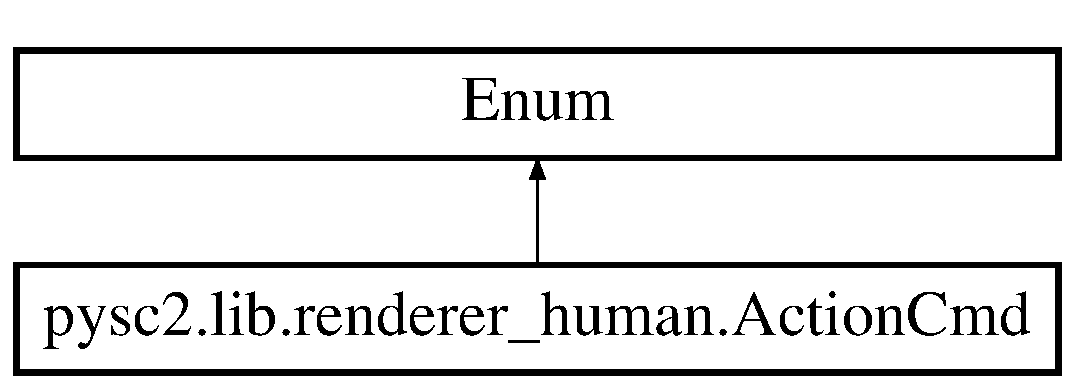
\includegraphics[height=2.000000cm]{classpysc2_1_1lib_1_1renderer__human_1_1_action_cmd}
\end{center}
\end{figure}
\subsection*{Static Public Attributes}
\begin{DoxyCompactItemize}
\item 
int \mbox{\hyperlink{classpysc2_1_1lib_1_1renderer__human_1_1_action_cmd_a481c5c5b3a9a827342d2dfa3d9f051f8}{S\+T\+EP}} = 1
\item 
int \mbox{\hyperlink{classpysc2_1_1lib_1_1renderer__human_1_1_action_cmd_a41f806188a045304567cbe763e982904}{R\+E\+S\+T\+A\+RT}} = 2
\item 
int \mbox{\hyperlink{classpysc2_1_1lib_1_1renderer__human_1_1_action_cmd_ae18886cbd175c7d2627fc1963bcf3695}{Q\+U\+IT}} = 3
\end{DoxyCompactItemize}


\subsection{Member Data Documentation}
\mbox{\Hypertarget{classpysc2_1_1lib_1_1renderer__human_1_1_action_cmd_ae18886cbd175c7d2627fc1963bcf3695}\label{classpysc2_1_1lib_1_1renderer__human_1_1_action_cmd_ae18886cbd175c7d2627fc1963bcf3695}} 
\index{pysc2\+::lib\+::renderer\+\_\+human\+::\+Action\+Cmd@{pysc2\+::lib\+::renderer\+\_\+human\+::\+Action\+Cmd}!Q\+U\+IT@{Q\+U\+IT}}
\index{Q\+U\+IT@{Q\+U\+IT}!pysc2\+::lib\+::renderer\+\_\+human\+::\+Action\+Cmd@{pysc2\+::lib\+::renderer\+\_\+human\+::\+Action\+Cmd}}
\subsubsection{\texorpdfstring{Q\+U\+IT}{QUIT}}
{\footnotesize\ttfamily int pysc2.\+lib.\+renderer\+\_\+human.\+Action\+Cmd.\+Q\+U\+IT = 3\hspace{0.3cm}{\ttfamily [static]}}

\mbox{\Hypertarget{classpysc2_1_1lib_1_1renderer__human_1_1_action_cmd_a41f806188a045304567cbe763e982904}\label{classpysc2_1_1lib_1_1renderer__human_1_1_action_cmd_a41f806188a045304567cbe763e982904}} 
\index{pysc2\+::lib\+::renderer\+\_\+human\+::\+Action\+Cmd@{pysc2\+::lib\+::renderer\+\_\+human\+::\+Action\+Cmd}!R\+E\+S\+T\+A\+RT@{R\+E\+S\+T\+A\+RT}}
\index{R\+E\+S\+T\+A\+RT@{R\+E\+S\+T\+A\+RT}!pysc2\+::lib\+::renderer\+\_\+human\+::\+Action\+Cmd@{pysc2\+::lib\+::renderer\+\_\+human\+::\+Action\+Cmd}}
\subsubsection{\texorpdfstring{R\+E\+S\+T\+A\+RT}{RESTART}}
{\footnotesize\ttfamily int pysc2.\+lib.\+renderer\+\_\+human.\+Action\+Cmd.\+R\+E\+S\+T\+A\+RT = 2\hspace{0.3cm}{\ttfamily [static]}}

\mbox{\Hypertarget{classpysc2_1_1lib_1_1renderer__human_1_1_action_cmd_a481c5c5b3a9a827342d2dfa3d9f051f8}\label{classpysc2_1_1lib_1_1renderer__human_1_1_action_cmd_a481c5c5b3a9a827342d2dfa3d9f051f8}} 
\index{pysc2\+::lib\+::renderer\+\_\+human\+::\+Action\+Cmd@{pysc2\+::lib\+::renderer\+\_\+human\+::\+Action\+Cmd}!S\+T\+EP@{S\+T\+EP}}
\index{S\+T\+EP@{S\+T\+EP}!pysc2\+::lib\+::renderer\+\_\+human\+::\+Action\+Cmd@{pysc2\+::lib\+::renderer\+\_\+human\+::\+Action\+Cmd}}
\subsubsection{\texorpdfstring{S\+T\+EP}{STEP}}
{\footnotesize\ttfamily int pysc2.\+lib.\+renderer\+\_\+human.\+Action\+Cmd.\+S\+T\+EP = 1\hspace{0.3cm}{\ttfamily [static]}}



The documentation for this class was generated from the following file\+:\begin{DoxyCompactItemize}
\item 
lib/\mbox{\hyperlink{renderer__human_8py}{renderer\+\_\+human.\+py}}\end{DoxyCompactItemize}

\hypertarget{classpysc2_1_1lib_1_1actions_1_1_action_space}{}\section{pysc2.\+lib.\+actions.\+Action\+Space Class Reference}
\label{classpysc2_1_1lib_1_1actions_1_1_action_space}\index{pysc2.\+lib.\+actions.\+Action\+Space@{pysc2.\+lib.\+actions.\+Action\+Space}}
Inheritance diagram for pysc2.\+lib.\+actions.\+Action\+Space\+:\begin{figure}[H]
\begin{center}
\leavevmode
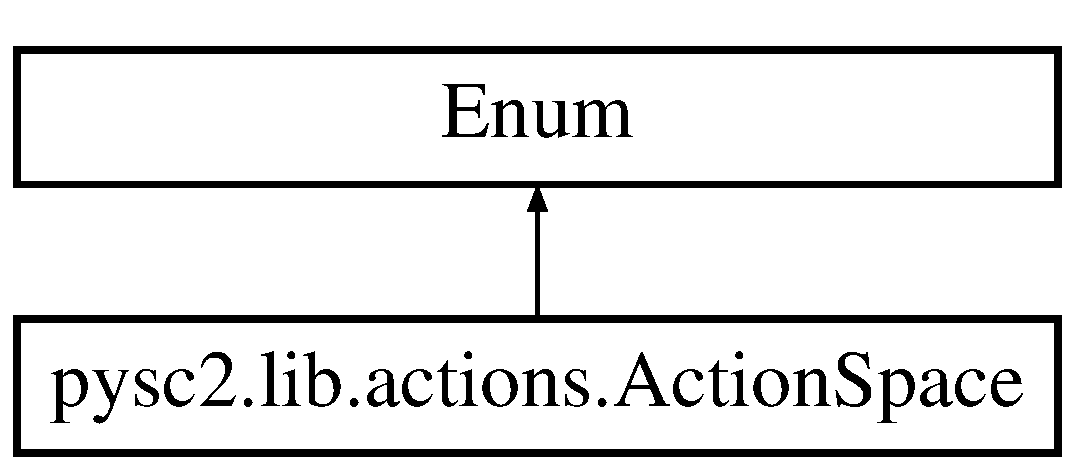
\includegraphics[height=2.000000cm]{classpysc2_1_1lib_1_1actions_1_1_action_space}
\end{center}
\end{figure}
\subsection*{Static Public Attributes}
\begin{DoxyCompactItemize}
\item 
int \mbox{\hyperlink{classpysc2_1_1lib_1_1actions_1_1_action_space_ac436954d571bb283b841d031f3805010}{F\+E\+A\+T\+U\+R\+ES}} = 1
\item 
int \mbox{\hyperlink{classpysc2_1_1lib_1_1actions_1_1_action_space_a4f7698070ca8cdf94697061cb83ad78a}{R\+GB}} = 2
\end{DoxyCompactItemize}


\subsection{Member Data Documentation}
\mbox{\Hypertarget{classpysc2_1_1lib_1_1actions_1_1_action_space_ac436954d571bb283b841d031f3805010}\label{classpysc2_1_1lib_1_1actions_1_1_action_space_ac436954d571bb283b841d031f3805010}} 
\index{pysc2\+::lib\+::actions\+::\+Action\+Space@{pysc2\+::lib\+::actions\+::\+Action\+Space}!F\+E\+A\+T\+U\+R\+ES@{F\+E\+A\+T\+U\+R\+ES}}
\index{F\+E\+A\+T\+U\+R\+ES@{F\+E\+A\+T\+U\+R\+ES}!pysc2\+::lib\+::actions\+::\+Action\+Space@{pysc2\+::lib\+::actions\+::\+Action\+Space}}
\subsubsection{\texorpdfstring{F\+E\+A\+T\+U\+R\+ES}{FEATURES}}
{\footnotesize\ttfamily int pysc2.\+lib.\+actions.\+Action\+Space.\+F\+E\+A\+T\+U\+R\+ES = 1\hspace{0.3cm}{\ttfamily [static]}}

\mbox{\Hypertarget{classpysc2_1_1lib_1_1actions_1_1_action_space_a4f7698070ca8cdf94697061cb83ad78a}\label{classpysc2_1_1lib_1_1actions_1_1_action_space_a4f7698070ca8cdf94697061cb83ad78a}} 
\index{pysc2\+::lib\+::actions\+::\+Action\+Space@{pysc2\+::lib\+::actions\+::\+Action\+Space}!R\+GB@{R\+GB}}
\index{R\+GB@{R\+GB}!pysc2\+::lib\+::actions\+::\+Action\+Space@{pysc2\+::lib\+::actions\+::\+Action\+Space}}
\subsubsection{\texorpdfstring{R\+GB}{RGB}}
{\footnotesize\ttfamily int pysc2.\+lib.\+actions.\+Action\+Space.\+R\+GB = 2\hspace{0.3cm}{\ttfamily [static]}}



The documentation for this class was generated from the following file\+:\begin{DoxyCompactItemize}
\item 
lib/\mbox{\hyperlink{actions_8py}{actions.\+py}}\end{DoxyCompactItemize}

\hypertarget{classpysc2_1_1env_1_1lan__sc2__env_1_1_addr}{}\section{pysc2.\+env.\+lan\+\_\+sc2\+\_\+env.\+Addr Class Reference}
\label{classpysc2_1_1env_1_1lan__sc2__env_1_1_addr}\index{pysc2.\+env.\+lan\+\_\+sc2\+\_\+env.\+Addr@{pysc2.\+env.\+lan\+\_\+sc2\+\_\+env.\+Addr}}
Inheritance diagram for pysc2.\+env.\+lan\+\_\+sc2\+\_\+env.\+Addr\+:\begin{figure}[H]
\begin{center}
\leavevmode
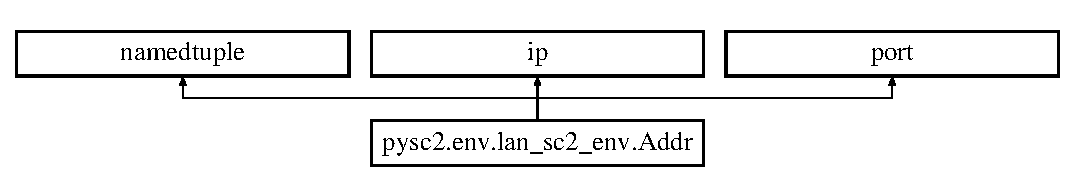
\includegraphics[height=1.996435cm]{classpysc2_1_1env_1_1lan__sc2__env_1_1_addr}
\end{center}
\end{figure}
\subsection*{Public Member Functions}
\begin{DoxyCompactItemize}
\item 
def \mbox{\hyperlink{classpysc2_1_1env_1_1lan__sc2__env_1_1_addr_a7365bf76a5c653b039ec16e22360a7b3}{\+\_\+\+\_\+str\+\_\+\+\_\+}} (self)
\end{DoxyCompactItemize}


\subsection{Member Function Documentation}
\mbox{\Hypertarget{classpysc2_1_1env_1_1lan__sc2__env_1_1_addr_a7365bf76a5c653b039ec16e22360a7b3}\label{classpysc2_1_1env_1_1lan__sc2__env_1_1_addr_a7365bf76a5c653b039ec16e22360a7b3}} 
\index{pysc2\+::env\+::lan\+\_\+sc2\+\_\+env\+::\+Addr@{pysc2\+::env\+::lan\+\_\+sc2\+\_\+env\+::\+Addr}!\+\_\+\+\_\+str\+\_\+\+\_\+@{\+\_\+\+\_\+str\+\_\+\+\_\+}}
\index{\+\_\+\+\_\+str\+\_\+\+\_\+@{\+\_\+\+\_\+str\+\_\+\+\_\+}!pysc2\+::env\+::lan\+\_\+sc2\+\_\+env\+::\+Addr@{pysc2\+::env\+::lan\+\_\+sc2\+\_\+env\+::\+Addr}}
\subsubsection{\texorpdfstring{\+\_\+\+\_\+str\+\_\+\+\_\+()}{\_\_str\_\_()}}
{\footnotesize\ttfamily def pysc2.\+env.\+lan\+\_\+sc2\+\_\+env.\+Addr.\+\_\+\+\_\+str\+\_\+\+\_\+ (\begin{DoxyParamCaption}\item[{}]{self }\end{DoxyParamCaption})}



The documentation for this class was generated from the following file\+:\begin{DoxyCompactItemize}
\item 
env/\mbox{\hyperlink{lan__sc2__env_8py}{lan\+\_\+sc2\+\_\+env.\+py}}\end{DoxyCompactItemize}

\hypertarget{classpysc2_1_1lib_1_1features_1_1_agent_interface_format}{}\section{pysc2.\+lib.\+features.\+Agent\+Interface\+Format Class Reference}
\label{classpysc2_1_1lib_1_1features_1_1_agent_interface_format}\index{pysc2.\+lib.\+features.\+Agent\+Interface\+Format@{pysc2.\+lib.\+features.\+Agent\+Interface\+Format}}
Inheritance diagram for pysc2.\+lib.\+features.\+Agent\+Interface\+Format\+:\begin{figure}[H]
\begin{center}
\leavevmode
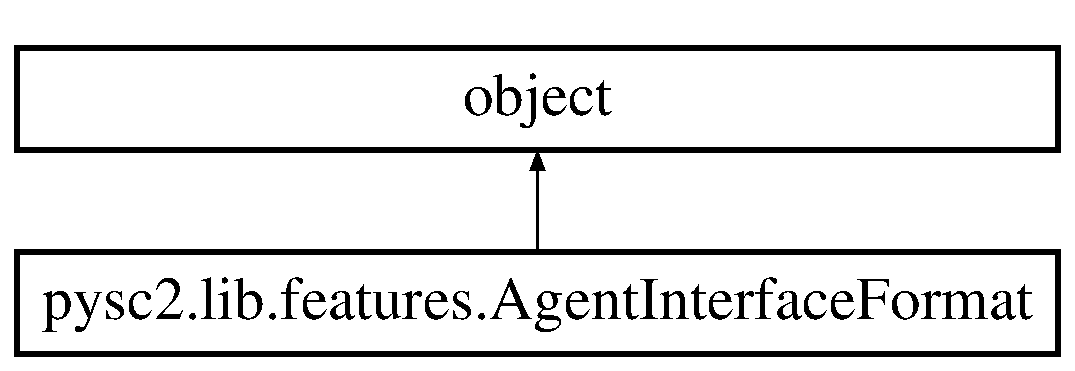
\includegraphics[height=2.000000cm]{classpysc2_1_1lib_1_1features_1_1_agent_interface_format}
\end{center}
\end{figure}
\subsection*{Public Member Functions}
\begin{DoxyCompactItemize}
\item 
def \mbox{\hyperlink{classpysc2_1_1lib_1_1features_1_1_agent_interface_format_a80c173fac4f02ee090925b0ba2eaa369}{\+\_\+\+\_\+init\+\_\+\+\_\+}} (self, \mbox{\hyperlink{classpysc2_1_1lib_1_1features_1_1_agent_interface_format_afb6336f68b4dd6a550a8483e59d8bf31}{feature\+\_\+dimensions}}=None, \mbox{\hyperlink{classpysc2_1_1lib_1_1features_1_1_agent_interface_format_a5531c5661ecd91f244bf3f9598d22d67}{rgb\+\_\+dimensions}}=None, \mbox{\hyperlink{classpysc2_1_1lib_1_1features_1_1_agent_interface_format_aebb7cd1ed5816051abe21703184cc16a}{action\+\_\+space}}=None, \mbox{\hyperlink{classpysc2_1_1lib_1_1features_1_1_agent_interface_format_a5140a9024f2fb47046074e511acd0dd0}{camera\+\_\+width\+\_\+world\+\_\+units}}=None, \mbox{\hyperlink{classpysc2_1_1lib_1_1features_1_1_agent_interface_format_abac891fe53cafd4798d13ca70db971f5}{use\+\_\+feature\+\_\+units}}=False, \mbox{\hyperlink{classpysc2_1_1lib_1_1features_1_1_agent_interface_format_adbc6be15eae7945c226758c1bc666443}{hide\+\_\+specific\+\_\+actions}}=True)
\item 
def \mbox{\hyperlink{classpysc2_1_1lib_1_1features_1_1_agent_interface_format_afb6336f68b4dd6a550a8483e59d8bf31}{feature\+\_\+dimensions}} (self)
\item 
def \mbox{\hyperlink{classpysc2_1_1lib_1_1features_1_1_agent_interface_format_a5531c5661ecd91f244bf3f9598d22d67}{rgb\+\_\+dimensions}} (self)
\item 
def \mbox{\hyperlink{classpysc2_1_1lib_1_1features_1_1_agent_interface_format_aebb7cd1ed5816051abe21703184cc16a}{action\+\_\+space}} (self)
\item 
def \mbox{\hyperlink{classpysc2_1_1lib_1_1features_1_1_agent_interface_format_a5140a9024f2fb47046074e511acd0dd0}{camera\+\_\+width\+\_\+world\+\_\+units}} (self)
\item 
def \mbox{\hyperlink{classpysc2_1_1lib_1_1features_1_1_agent_interface_format_abac891fe53cafd4798d13ca70db971f5}{use\+\_\+feature\+\_\+units}} (self)
\item 
def \mbox{\hyperlink{classpysc2_1_1lib_1_1features_1_1_agent_interface_format_adbc6be15eae7945c226758c1bc666443}{hide\+\_\+specific\+\_\+actions}} (self)
\item 
def \mbox{\hyperlink{classpysc2_1_1lib_1_1features_1_1_agent_interface_format_a8fa5a036defb7844b94946a505e28148}{action\+\_\+dimensions}} (self)
\end{DoxyCompactItemize}


\subsection{Detailed Description}
\begin{DoxyVerb}Observation and action interface format specific to a particular agent.\end{DoxyVerb}
 

\subsection{Constructor \& Destructor Documentation}
\mbox{\Hypertarget{classpysc2_1_1lib_1_1features_1_1_agent_interface_format_a80c173fac4f02ee090925b0ba2eaa369}\label{classpysc2_1_1lib_1_1features_1_1_agent_interface_format_a80c173fac4f02ee090925b0ba2eaa369}} 
\index{pysc2\+::lib\+::features\+::\+Agent\+Interface\+Format@{pysc2\+::lib\+::features\+::\+Agent\+Interface\+Format}!\+\_\+\+\_\+init\+\_\+\+\_\+@{\+\_\+\+\_\+init\+\_\+\+\_\+}}
\index{\+\_\+\+\_\+init\+\_\+\+\_\+@{\+\_\+\+\_\+init\+\_\+\+\_\+}!pysc2\+::lib\+::features\+::\+Agent\+Interface\+Format@{pysc2\+::lib\+::features\+::\+Agent\+Interface\+Format}}
\subsubsection{\texorpdfstring{\+\_\+\+\_\+init\+\_\+\+\_\+()}{\_\_init\_\_()}}
{\footnotesize\ttfamily def pysc2.\+lib.\+features.\+Agent\+Interface\+Format.\+\_\+\+\_\+init\+\_\+\+\_\+ (\begin{DoxyParamCaption}\item[{}]{self,  }\item[{}]{feature\+\_\+dimensions = {\ttfamily None},  }\item[{}]{rgb\+\_\+dimensions = {\ttfamily None},  }\item[{}]{action\+\_\+space = {\ttfamily None},  }\item[{}]{camera\+\_\+width\+\_\+world\+\_\+units = {\ttfamily None},  }\item[{}]{use\+\_\+feature\+\_\+units = {\ttfamily False},  }\item[{}]{hide\+\_\+specific\+\_\+actions = {\ttfamily True} }\end{DoxyParamCaption})}

\begin{DoxyVerb}Initializer.

Args:
  feature_dimensions: Feature layer `Dimension`s. Either this or
  rgb_dimensions (or both) must be set.
  rgb_dimensions: RGB `Dimension`. Either this or feature_dimensions
  (or both) must be set.
  action_space: If you pass both feature and rgb sizes, then you must also
  specify which you want to use for your actions as an ActionSpace enum.
  camera_width_world_units: The width of your screen in world units. If your
  feature_dimensions.screen=(64, 48) and camera_width is 24, then each
  px represents 24 / 64 = 0.375 world units in each of x and y.
  It'll then represent a camera of size (24, 0.375 * 48) = (24, 18)
  world units.
  use_feature_units: Whether to include feature unit data in observations.
  hide_specific_actions: [bool] Some actions (eg cancel) have many
  specific versions (cancel this building, cancel that spell) and can
  be represented in a more general form. If a specific action is
  available, the general will also be available. If you set
  `hide_specific_actions` to False, the specific versions will also be
  available, but if it's True, the specific ones will be hidden.
  Similarly, when transforming back, a specific action will be returned
  as the general action. This simplifies the action space, though can
  lead to some actions in replays not being exactly representable using
  only the general actions.

Raises:
  ValueError: if the parameters are inconsistent.
\end{DoxyVerb}
 

\subsection{Member Function Documentation}
\mbox{\Hypertarget{classpysc2_1_1lib_1_1features_1_1_agent_interface_format_a8fa5a036defb7844b94946a505e28148}\label{classpysc2_1_1lib_1_1features_1_1_agent_interface_format_a8fa5a036defb7844b94946a505e28148}} 
\index{pysc2\+::lib\+::features\+::\+Agent\+Interface\+Format@{pysc2\+::lib\+::features\+::\+Agent\+Interface\+Format}!action\+\_\+dimensions@{action\+\_\+dimensions}}
\index{action\+\_\+dimensions@{action\+\_\+dimensions}!pysc2\+::lib\+::features\+::\+Agent\+Interface\+Format@{pysc2\+::lib\+::features\+::\+Agent\+Interface\+Format}}
\subsubsection{\texorpdfstring{action\+\_\+dimensions()}{action\_dimensions()}}
{\footnotesize\ttfamily def pysc2.\+lib.\+features.\+Agent\+Interface\+Format.\+action\+\_\+dimensions (\begin{DoxyParamCaption}\item[{}]{self }\end{DoxyParamCaption})}

\mbox{\Hypertarget{classpysc2_1_1lib_1_1features_1_1_agent_interface_format_aebb7cd1ed5816051abe21703184cc16a}\label{classpysc2_1_1lib_1_1features_1_1_agent_interface_format_aebb7cd1ed5816051abe21703184cc16a}} 
\index{pysc2\+::lib\+::features\+::\+Agent\+Interface\+Format@{pysc2\+::lib\+::features\+::\+Agent\+Interface\+Format}!action\+\_\+space@{action\+\_\+space}}
\index{action\+\_\+space@{action\+\_\+space}!pysc2\+::lib\+::features\+::\+Agent\+Interface\+Format@{pysc2\+::lib\+::features\+::\+Agent\+Interface\+Format}}
\subsubsection{\texorpdfstring{action\+\_\+space()}{action\_space()}}
{\footnotesize\ttfamily def pysc2.\+lib.\+features.\+Agent\+Interface\+Format.\+action\+\_\+space (\begin{DoxyParamCaption}\item[{}]{self }\end{DoxyParamCaption})}

\mbox{\Hypertarget{classpysc2_1_1lib_1_1features_1_1_agent_interface_format_a5140a9024f2fb47046074e511acd0dd0}\label{classpysc2_1_1lib_1_1features_1_1_agent_interface_format_a5140a9024f2fb47046074e511acd0dd0}} 
\index{pysc2\+::lib\+::features\+::\+Agent\+Interface\+Format@{pysc2\+::lib\+::features\+::\+Agent\+Interface\+Format}!camera\+\_\+width\+\_\+world\+\_\+units@{camera\+\_\+width\+\_\+world\+\_\+units}}
\index{camera\+\_\+width\+\_\+world\+\_\+units@{camera\+\_\+width\+\_\+world\+\_\+units}!pysc2\+::lib\+::features\+::\+Agent\+Interface\+Format@{pysc2\+::lib\+::features\+::\+Agent\+Interface\+Format}}
\subsubsection{\texorpdfstring{camera\+\_\+width\+\_\+world\+\_\+units()}{camera\_width\_world\_units()}}
{\footnotesize\ttfamily def pysc2.\+lib.\+features.\+Agent\+Interface\+Format.\+camera\+\_\+width\+\_\+world\+\_\+units (\begin{DoxyParamCaption}\item[{}]{self }\end{DoxyParamCaption})}

\mbox{\Hypertarget{classpysc2_1_1lib_1_1features_1_1_agent_interface_format_afb6336f68b4dd6a550a8483e59d8bf31}\label{classpysc2_1_1lib_1_1features_1_1_agent_interface_format_afb6336f68b4dd6a550a8483e59d8bf31}} 
\index{pysc2\+::lib\+::features\+::\+Agent\+Interface\+Format@{pysc2\+::lib\+::features\+::\+Agent\+Interface\+Format}!feature\+\_\+dimensions@{feature\+\_\+dimensions}}
\index{feature\+\_\+dimensions@{feature\+\_\+dimensions}!pysc2\+::lib\+::features\+::\+Agent\+Interface\+Format@{pysc2\+::lib\+::features\+::\+Agent\+Interface\+Format}}
\subsubsection{\texorpdfstring{feature\+\_\+dimensions()}{feature\_dimensions()}}
{\footnotesize\ttfamily def pysc2.\+lib.\+features.\+Agent\+Interface\+Format.\+feature\+\_\+dimensions (\begin{DoxyParamCaption}\item[{}]{self }\end{DoxyParamCaption})}

\mbox{\Hypertarget{classpysc2_1_1lib_1_1features_1_1_agent_interface_format_adbc6be15eae7945c226758c1bc666443}\label{classpysc2_1_1lib_1_1features_1_1_agent_interface_format_adbc6be15eae7945c226758c1bc666443}} 
\index{pysc2\+::lib\+::features\+::\+Agent\+Interface\+Format@{pysc2\+::lib\+::features\+::\+Agent\+Interface\+Format}!hide\+\_\+specific\+\_\+actions@{hide\+\_\+specific\+\_\+actions}}
\index{hide\+\_\+specific\+\_\+actions@{hide\+\_\+specific\+\_\+actions}!pysc2\+::lib\+::features\+::\+Agent\+Interface\+Format@{pysc2\+::lib\+::features\+::\+Agent\+Interface\+Format}}
\subsubsection{\texorpdfstring{hide\+\_\+specific\+\_\+actions()}{hide\_specific\_actions()}}
{\footnotesize\ttfamily def pysc2.\+lib.\+features.\+Agent\+Interface\+Format.\+hide\+\_\+specific\+\_\+actions (\begin{DoxyParamCaption}\item[{}]{self }\end{DoxyParamCaption})}

\mbox{\Hypertarget{classpysc2_1_1lib_1_1features_1_1_agent_interface_format_a5531c5661ecd91f244bf3f9598d22d67}\label{classpysc2_1_1lib_1_1features_1_1_agent_interface_format_a5531c5661ecd91f244bf3f9598d22d67}} 
\index{pysc2\+::lib\+::features\+::\+Agent\+Interface\+Format@{pysc2\+::lib\+::features\+::\+Agent\+Interface\+Format}!rgb\+\_\+dimensions@{rgb\+\_\+dimensions}}
\index{rgb\+\_\+dimensions@{rgb\+\_\+dimensions}!pysc2\+::lib\+::features\+::\+Agent\+Interface\+Format@{pysc2\+::lib\+::features\+::\+Agent\+Interface\+Format}}
\subsubsection{\texorpdfstring{rgb\+\_\+dimensions()}{rgb\_dimensions()}}
{\footnotesize\ttfamily def pysc2.\+lib.\+features.\+Agent\+Interface\+Format.\+rgb\+\_\+dimensions (\begin{DoxyParamCaption}\item[{}]{self }\end{DoxyParamCaption})}

\mbox{\Hypertarget{classpysc2_1_1lib_1_1features_1_1_agent_interface_format_abac891fe53cafd4798d13ca70db971f5}\label{classpysc2_1_1lib_1_1features_1_1_agent_interface_format_abac891fe53cafd4798d13ca70db971f5}} 
\index{pysc2\+::lib\+::features\+::\+Agent\+Interface\+Format@{pysc2\+::lib\+::features\+::\+Agent\+Interface\+Format}!use\+\_\+feature\+\_\+units@{use\+\_\+feature\+\_\+units}}
\index{use\+\_\+feature\+\_\+units@{use\+\_\+feature\+\_\+units}!pysc2\+::lib\+::features\+::\+Agent\+Interface\+Format@{pysc2\+::lib\+::features\+::\+Agent\+Interface\+Format}}
\subsubsection{\texorpdfstring{use\+\_\+feature\+\_\+units()}{use\_feature\_units()}}
{\footnotesize\ttfamily def pysc2.\+lib.\+features.\+Agent\+Interface\+Format.\+use\+\_\+feature\+\_\+units (\begin{DoxyParamCaption}\item[{}]{self }\end{DoxyParamCaption})}



The documentation for this class was generated from the following file\+:\begin{DoxyCompactItemize}
\item 
lib/\mbox{\hyperlink{features_8py}{features.\+py}}\end{DoxyCompactItemize}

\hypertarget{classpysc2_1_1lib_1_1actions_1_1_arguments}{}\section{pysc2.\+lib.\+actions.\+Arguments Class Reference}
\label{classpysc2_1_1lib_1_1actions_1_1_arguments}\index{pysc2.\+lib.\+actions.\+Arguments@{pysc2.\+lib.\+actions.\+Arguments}}
Inheritance diagram for pysc2.\+lib.\+actions.\+Arguments\+:\begin{figure}[H]
\begin{center}
\leavevmode
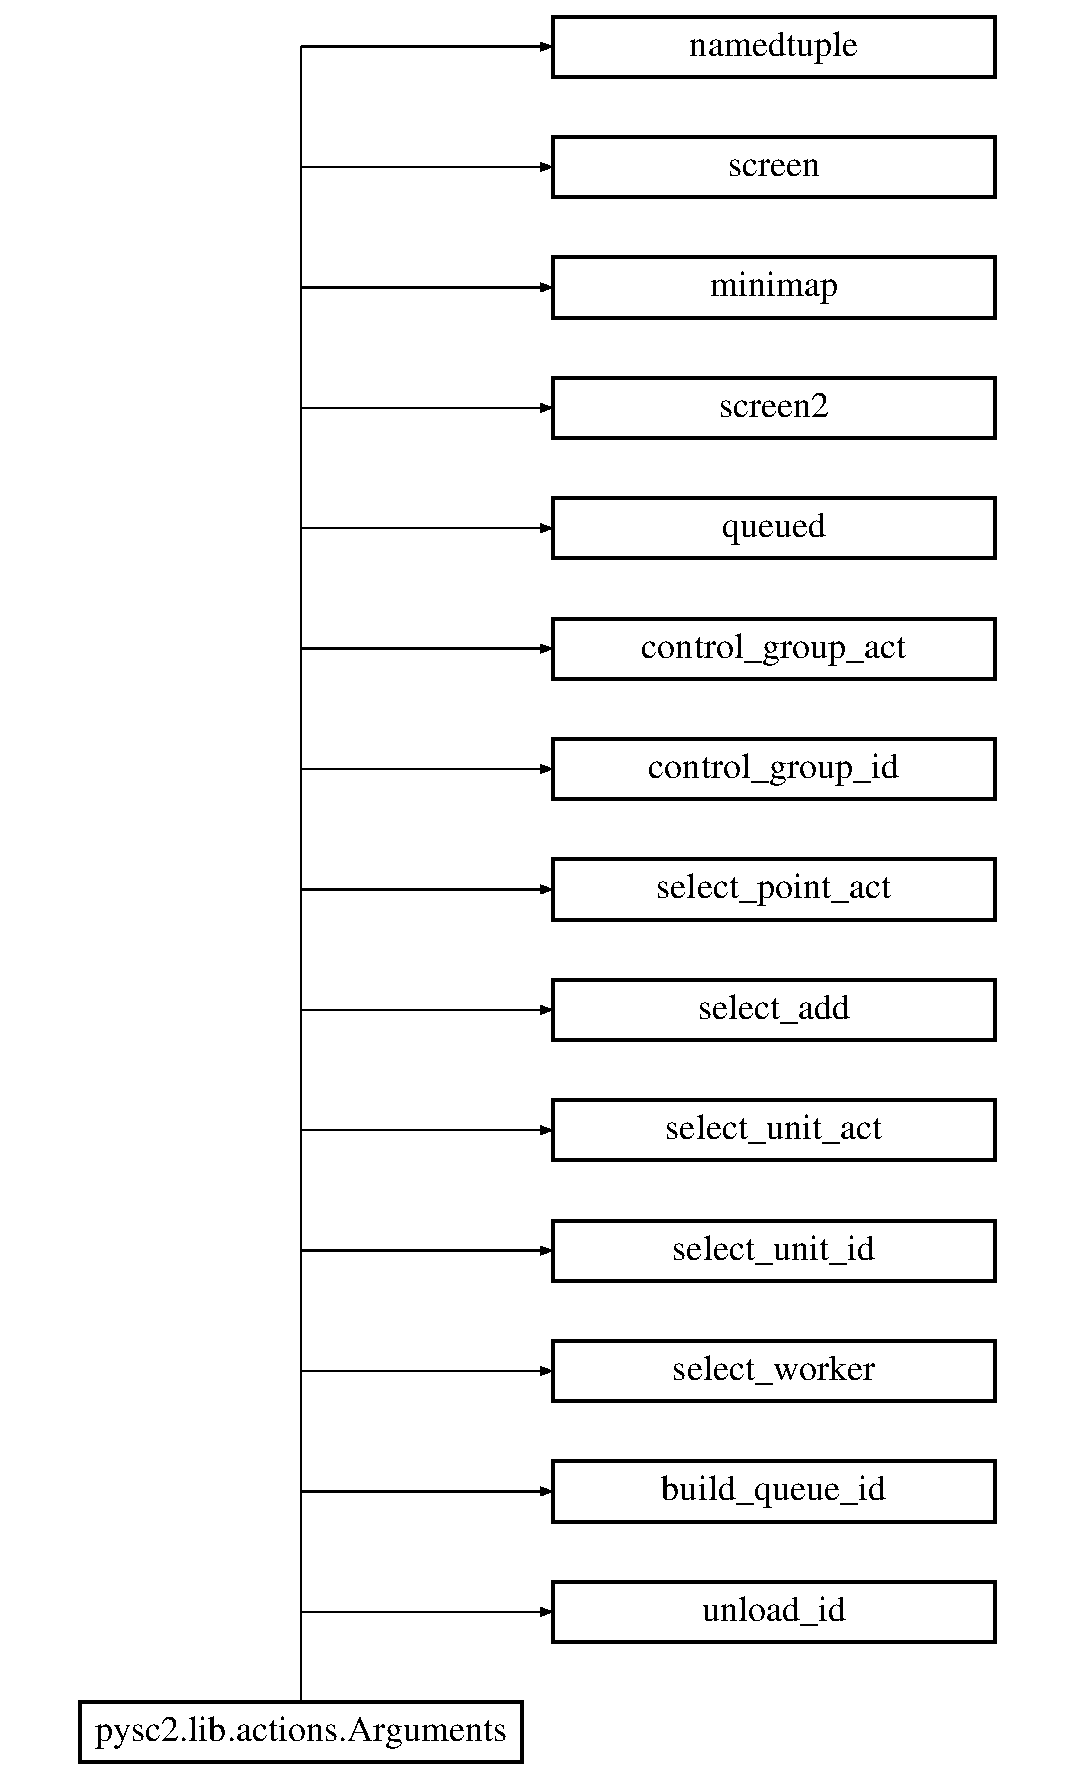
\includegraphics[height=12.000000cm]{classpysc2_1_1lib_1_1actions_1_1_arguments}
\end{center}
\end{figure}
\subsection*{Public Member Functions}
\begin{DoxyCompactItemize}
\item 
def \mbox{\hyperlink{classpysc2_1_1lib_1_1actions_1_1_arguments_ab78c631c19bfc340e35069612a5b1f22}{types}} (cls, kwargs)
\end{DoxyCompactItemize}


\subsection{Detailed Description}
\begin{DoxyVerb}The full list of argument types.

Take a look at TYPES and FUNCTION_TYPES for more details.

Attributes:
  screen: A point on the screen.
  minimap: A point on the minimap.
  screen2: The second point for a rectangle. This is needed so that no
      function takes the same type twice.
  queued: Whether the action should be done now or later.
  control_group_act: What to do with the control group.
  control_group_id: Which control group to do it with.
  select_point_act: What to do with the unit at the point.
  select_add: Whether to add the unit to the selection or replace it.
  select_unit_act: What to do when selecting a unit by id.
  select_unit_id: Which unit to select by id.
  select_worker: What to do when selecting a worker.
  build_queue_id: Which build queue index to target.
  unload_id: Which unit to target in a transport/nydus/command center.
\end{DoxyVerb}
 

\subsection{Member Function Documentation}
\mbox{\Hypertarget{classpysc2_1_1lib_1_1actions_1_1_arguments_ab78c631c19bfc340e35069612a5b1f22}\label{classpysc2_1_1lib_1_1actions_1_1_arguments_ab78c631c19bfc340e35069612a5b1f22}} 
\index{pysc2\+::lib\+::actions\+::\+Arguments@{pysc2\+::lib\+::actions\+::\+Arguments}!types@{types}}
\index{types@{types}!pysc2\+::lib\+::actions\+::\+Arguments@{pysc2\+::lib\+::actions\+::\+Arguments}}
\subsubsection{\texorpdfstring{types()}{types()}}
{\footnotesize\ttfamily def pysc2.\+lib.\+actions.\+Arguments.\+types (\begin{DoxyParamCaption}\item[{}]{cls,  }\item[{}]{kwargs }\end{DoxyParamCaption})}

\begin{DoxyVerb}Create an Arguments of the possible Types.\end{DoxyVerb}
 

The documentation for this class was generated from the following file\+:\begin{DoxyCompactItemize}
\item 
lib/\mbox{\hyperlink{actions_8py}{actions.\+py}}\end{DoxyCompactItemize}

\hypertarget{classpysc2_1_1lib_1_1actions_1_1_argument_type}{}\section{pysc2.\+lib.\+actions.\+Argument\+Type Class Reference}
\label{classpysc2_1_1lib_1_1actions_1_1_argument_type}\index{pysc2.\+lib.\+actions.\+Argument\+Type@{pysc2.\+lib.\+actions.\+Argument\+Type}}
Inheritance diagram for pysc2.\+lib.\+actions.\+Argument\+Type\+:\begin{figure}[H]
\begin{center}
\leavevmode
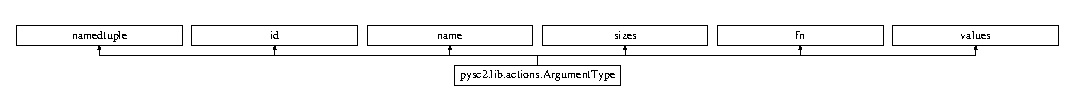
\includegraphics[height=0.928690cm]{classpysc2_1_1lib_1_1actions_1_1_argument_type}
\end{center}
\end{figure}
\subsection*{Public Member Functions}
\begin{DoxyCompactItemize}
\item 
def \mbox{\hyperlink{classpysc2_1_1lib_1_1actions_1_1_argument_type_a9adbb0aefcb2fc39e36b1c718889f9cc}{\+\_\+\+\_\+str\+\_\+\+\_\+}} (self)
\item 
def \mbox{\hyperlink{classpysc2_1_1lib_1_1actions_1_1_argument_type_a7b139c13ef12cd5bffa45c09af082140}{enum}} (cls, options, values)
\item 
def \mbox{\hyperlink{classpysc2_1_1lib_1_1actions_1_1_argument_type_a6440b4d3ca6308d338405b4dd456abab}{scalar}} (cls, value)
\item 
def \mbox{\hyperlink{classpysc2_1_1lib_1_1actions_1_1_argument_type_acd7c52464b761ade90cc6d63957a0739}{point}} (cls)
\item 
def \mbox{\hyperlink{classpysc2_1_1lib_1_1actions_1_1_argument_type_abeda01e4e7ab3656447b9b4af4ed26d3}{spec}} (cls, id\+\_\+, name, sizes)
\end{DoxyCompactItemize}


\subsection{Detailed Description}
\begin{DoxyVerb}Represents a single argument type.

Attributes:
  id: The argument id. This is unique.
  name: The name of the argument, also unique.
  sizes: The max+1 of each of the dimensions this argument takes.
  fn: The function to convert the list of integers into something more
      meaningful to be set in the protos to send to the game.
  values: An enum representing the values this argument type could hold. None
      if this isn't an enum argument type.
\end{DoxyVerb}
 

\subsection{Member Function Documentation}
\mbox{\Hypertarget{classpysc2_1_1lib_1_1actions_1_1_argument_type_a9adbb0aefcb2fc39e36b1c718889f9cc}\label{classpysc2_1_1lib_1_1actions_1_1_argument_type_a9adbb0aefcb2fc39e36b1c718889f9cc}} 
\index{pysc2\+::lib\+::actions\+::\+Argument\+Type@{pysc2\+::lib\+::actions\+::\+Argument\+Type}!\+\_\+\+\_\+str\+\_\+\+\_\+@{\+\_\+\+\_\+str\+\_\+\+\_\+}}
\index{\+\_\+\+\_\+str\+\_\+\+\_\+@{\+\_\+\+\_\+str\+\_\+\+\_\+}!pysc2\+::lib\+::actions\+::\+Argument\+Type@{pysc2\+::lib\+::actions\+::\+Argument\+Type}}
\subsubsection{\texorpdfstring{\+\_\+\+\_\+str\+\_\+\+\_\+()}{\_\_str\_\_()}}
{\footnotesize\ttfamily def pysc2.\+lib.\+actions.\+Argument\+Type.\+\_\+\+\_\+str\+\_\+\+\_\+ (\begin{DoxyParamCaption}\item[{}]{self }\end{DoxyParamCaption})}

\mbox{\Hypertarget{classpysc2_1_1lib_1_1actions_1_1_argument_type_a7b139c13ef12cd5bffa45c09af082140}\label{classpysc2_1_1lib_1_1actions_1_1_argument_type_a7b139c13ef12cd5bffa45c09af082140}} 
\index{pysc2\+::lib\+::actions\+::\+Argument\+Type@{pysc2\+::lib\+::actions\+::\+Argument\+Type}!enum@{enum}}
\index{enum@{enum}!pysc2\+::lib\+::actions\+::\+Argument\+Type@{pysc2\+::lib\+::actions\+::\+Argument\+Type}}
\subsubsection{\texorpdfstring{enum()}{enum()}}
{\footnotesize\ttfamily def pysc2.\+lib.\+actions.\+Argument\+Type.\+enum (\begin{DoxyParamCaption}\item[{}]{cls,  }\item[{}]{options,  }\item[{}]{values }\end{DoxyParamCaption})}

\begin{DoxyVerb}Create an ArgumentType where you choose one of a set of known values.\end{DoxyVerb}
 \mbox{\Hypertarget{classpysc2_1_1lib_1_1actions_1_1_argument_type_acd7c52464b761ade90cc6d63957a0739}\label{classpysc2_1_1lib_1_1actions_1_1_argument_type_acd7c52464b761ade90cc6d63957a0739}} 
\index{pysc2\+::lib\+::actions\+::\+Argument\+Type@{pysc2\+::lib\+::actions\+::\+Argument\+Type}!point@{point}}
\index{point@{point}!pysc2\+::lib\+::actions\+::\+Argument\+Type@{pysc2\+::lib\+::actions\+::\+Argument\+Type}}
\subsubsection{\texorpdfstring{point()}{point()}}
{\footnotesize\ttfamily def pysc2.\+lib.\+actions.\+Argument\+Type.\+point (\begin{DoxyParamCaption}\item[{}]{cls }\end{DoxyParamCaption})}

\begin{DoxyVerb}Create an ArgumentType that is represented by a point.Point.\end{DoxyVerb}
 \mbox{\Hypertarget{classpysc2_1_1lib_1_1actions_1_1_argument_type_a6440b4d3ca6308d338405b4dd456abab}\label{classpysc2_1_1lib_1_1actions_1_1_argument_type_a6440b4d3ca6308d338405b4dd456abab}} 
\index{pysc2\+::lib\+::actions\+::\+Argument\+Type@{pysc2\+::lib\+::actions\+::\+Argument\+Type}!scalar@{scalar}}
\index{scalar@{scalar}!pysc2\+::lib\+::actions\+::\+Argument\+Type@{pysc2\+::lib\+::actions\+::\+Argument\+Type}}
\subsubsection{\texorpdfstring{scalar()}{scalar()}}
{\footnotesize\ttfamily def pysc2.\+lib.\+actions.\+Argument\+Type.\+scalar (\begin{DoxyParamCaption}\item[{}]{cls,  }\item[{}]{value }\end{DoxyParamCaption})}

\begin{DoxyVerb}Create an ArgumentType with a single scalar in range(value).\end{DoxyVerb}
 \mbox{\Hypertarget{classpysc2_1_1lib_1_1actions_1_1_argument_type_abeda01e4e7ab3656447b9b4af4ed26d3}\label{classpysc2_1_1lib_1_1actions_1_1_argument_type_abeda01e4e7ab3656447b9b4af4ed26d3}} 
\index{pysc2\+::lib\+::actions\+::\+Argument\+Type@{pysc2\+::lib\+::actions\+::\+Argument\+Type}!spec@{spec}}
\index{spec@{spec}!pysc2\+::lib\+::actions\+::\+Argument\+Type@{pysc2\+::lib\+::actions\+::\+Argument\+Type}}
\subsubsection{\texorpdfstring{spec()}{spec()}}
{\footnotesize\ttfamily def pysc2.\+lib.\+actions.\+Argument\+Type.\+spec (\begin{DoxyParamCaption}\item[{}]{cls,  }\item[{}]{id\+\_\+,  }\item[{}]{name,  }\item[{}]{sizes }\end{DoxyParamCaption})}

\begin{DoxyVerb}Create an ArgumentType to be used in ValidActions.\end{DoxyVerb}
 

The documentation for this class was generated from the following file\+:\begin{DoxyCompactItemize}
\item 
lib/\mbox{\hyperlink{actions_8py}{actions.\+py}}\end{DoxyCompactItemize}

\hypertarget{classpysc2_1_1env_1_1available__actions__printer_1_1_available_actions_printer}{}\section{pysc2.\+env.\+available\+\_\+actions\+\_\+printer.\+Available\+Actions\+Printer Class Reference}
\label{classpysc2_1_1env_1_1available__actions__printer_1_1_available_actions_printer}\index{pysc2.\+env.\+available\+\_\+actions\+\_\+printer.\+Available\+Actions\+Printer@{pysc2.\+env.\+available\+\_\+actions\+\_\+printer.\+Available\+Actions\+Printer}}
Inheritance diagram for pysc2.\+env.\+available\+\_\+actions\+\_\+printer.\+Available\+Actions\+Printer\+:\begin{figure}[H]
\begin{center}
\leavevmode
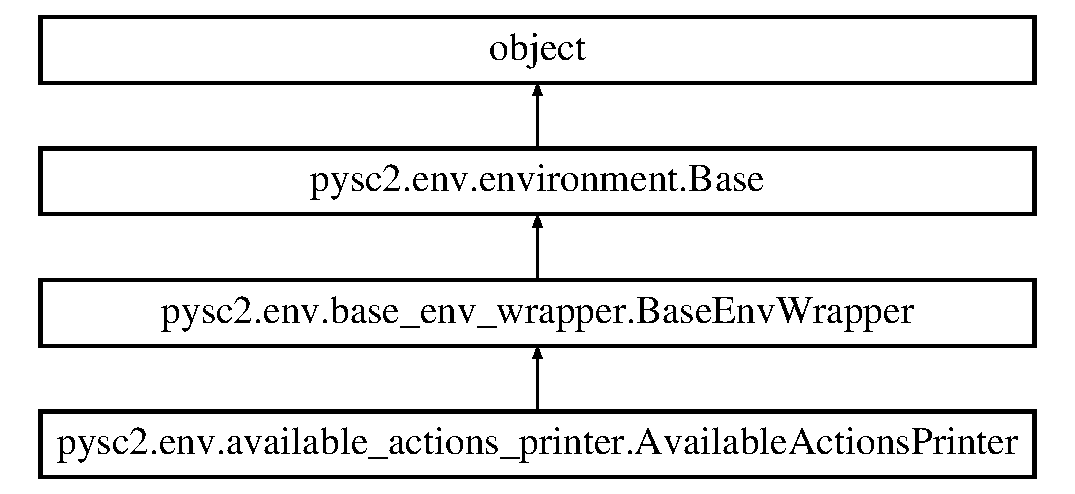
\includegraphics[height=4.000000cm]{classpysc2_1_1env_1_1available__actions__printer_1_1_available_actions_printer}
\end{center}
\end{figure}
\subsection*{Public Member Functions}
\begin{DoxyCompactItemize}
\item 
def \mbox{\hyperlink{classpysc2_1_1env_1_1available__actions__printer_1_1_available_actions_printer_a65c7b508da0d9b5c0b0f9e8bec02e5c3}{\+\_\+\+\_\+init\+\_\+\+\_\+}} (self, env)
\item 
def \mbox{\hyperlink{classpysc2_1_1env_1_1available__actions__printer_1_1_available_actions_printer_a4a58432803a5d2b7ea60107f71dc2d86}{step}} (self, args, kwargs)
\end{DoxyCompactItemize}


\subsection{Detailed Description}
\begin{DoxyVerb}An env wrapper to print the available actions.\end{DoxyVerb}
 

\subsection{Constructor \& Destructor Documentation}
\mbox{\Hypertarget{classpysc2_1_1env_1_1available__actions__printer_1_1_available_actions_printer_a65c7b508da0d9b5c0b0f9e8bec02e5c3}\label{classpysc2_1_1env_1_1available__actions__printer_1_1_available_actions_printer_a65c7b508da0d9b5c0b0f9e8bec02e5c3}} 
\index{pysc2\+::env\+::available\+\_\+actions\+\_\+printer\+::\+Available\+Actions\+Printer@{pysc2\+::env\+::available\+\_\+actions\+\_\+printer\+::\+Available\+Actions\+Printer}!\+\_\+\+\_\+init\+\_\+\+\_\+@{\+\_\+\+\_\+init\+\_\+\+\_\+}}
\index{\+\_\+\+\_\+init\+\_\+\+\_\+@{\+\_\+\+\_\+init\+\_\+\+\_\+}!pysc2\+::env\+::available\+\_\+actions\+\_\+printer\+::\+Available\+Actions\+Printer@{pysc2\+::env\+::available\+\_\+actions\+\_\+printer\+::\+Available\+Actions\+Printer}}
\subsubsection{\texorpdfstring{\+\_\+\+\_\+init\+\_\+\+\_\+()}{\_\_init\_\_()}}
{\footnotesize\ttfamily def pysc2.\+env.\+available\+\_\+actions\+\_\+printer.\+Available\+Actions\+Printer.\+\_\+\+\_\+init\+\_\+\+\_\+ (\begin{DoxyParamCaption}\item[{}]{self,  }\item[{}]{env }\end{DoxyParamCaption})}



\subsection{Member Function Documentation}
\mbox{\Hypertarget{classpysc2_1_1env_1_1available__actions__printer_1_1_available_actions_printer_a4a58432803a5d2b7ea60107f71dc2d86}\label{classpysc2_1_1env_1_1available__actions__printer_1_1_available_actions_printer_a4a58432803a5d2b7ea60107f71dc2d86}} 
\index{pysc2\+::env\+::available\+\_\+actions\+\_\+printer\+::\+Available\+Actions\+Printer@{pysc2\+::env\+::available\+\_\+actions\+\_\+printer\+::\+Available\+Actions\+Printer}!step@{step}}
\index{step@{step}!pysc2\+::env\+::available\+\_\+actions\+\_\+printer\+::\+Available\+Actions\+Printer@{pysc2\+::env\+::available\+\_\+actions\+\_\+printer\+::\+Available\+Actions\+Printer}}
\subsubsection{\texorpdfstring{step()}{step()}}
{\footnotesize\ttfamily def pysc2.\+env.\+available\+\_\+actions\+\_\+printer.\+Available\+Actions\+Printer.\+step (\begin{DoxyParamCaption}\item[{}]{self,  }\item[{}]{args,  }\item[{}]{kwargs }\end{DoxyParamCaption})}



The documentation for this class was generated from the following file\+:\begin{DoxyCompactItemize}
\item 
env/\mbox{\hyperlink{available__actions__printer_8py}{available\+\_\+actions\+\_\+printer.\+py}}\end{DoxyCompactItemize}

\hypertarget{classpysc2_1_1lib_1_1features__test_1_1_available_actions_test}{}\section{pysc2.\+lib.\+features\+\_\+test.\+Available\+Actions\+Test Class Reference}
\label{classpysc2_1_1lib_1_1features__test_1_1_available_actions_test}\index{pysc2.\+lib.\+features\+\_\+test.\+Available\+Actions\+Test@{pysc2.\+lib.\+features\+\_\+test.\+Available\+Actions\+Test}}
Inheritance diagram for pysc2.\+lib.\+features\+\_\+test.\+Available\+Actions\+Test\+:\begin{figure}[H]
\begin{center}
\leavevmode
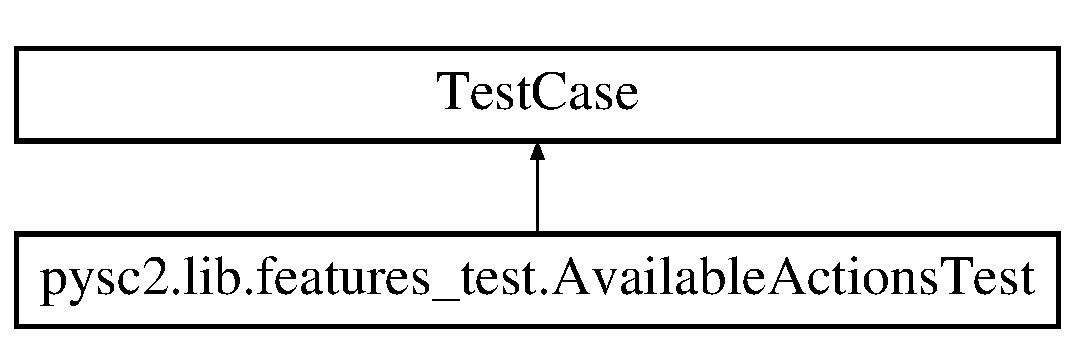
\includegraphics[height=2.000000cm]{classpysc2_1_1lib_1_1features__test_1_1_available_actions_test}
\end{center}
\end{figure}
\subsection*{Public Member Functions}
\begin{DoxyCompactItemize}
\item 
def \mbox{\hyperlink{classpysc2_1_1lib_1_1features__test_1_1_available_actions_test_a085183352ca922ab9a9c064bf97c2a29}{set\+Up}} (self)
\item 
def \mbox{\hyperlink{classpysc2_1_1lib_1_1features__test_1_1_available_actions_test_a1c9bfef603273fcfbdf206f7a0ef7620}{hide\+Specific\+Actions}} (self, hide\+\_\+specific\+\_\+actions)
\item 
def \mbox{\hyperlink{classpysc2_1_1lib_1_1features__test_1_1_available_actions_test_af4d9c7bad6bec5202f096d73cfc641b3}{assert\+Avail}} (self, expected)
\item 
def \mbox{\hyperlink{classpysc2_1_1lib_1_1features__test_1_1_available_actions_test_a2a9f056fe14cf0acb0bc47e4e1be6c61}{test\+Always}} (self)
\item 
def \mbox{\hyperlink{classpysc2_1_1lib_1_1features__test_1_1_available_actions_test_a5e280b23d7546871414c4eb0beced74b}{test\+Select\+Unit}} (self)
\item 
def \mbox{\hyperlink{classpysc2_1_1lib_1_1features__test_1_1_available_actions_test_ab667d51eb6a9b38da9ac0ababe007daf}{test\+Select\+Idle\+Workder}} (self)
\item 
def \mbox{\hyperlink{classpysc2_1_1lib_1_1features__test_1_1_available_actions_test_a0c4201958e89dce9568dc9f2d778ae5a}{test\+Select\+Army}} (self)
\item 
def \mbox{\hyperlink{classpysc2_1_1lib_1_1features__test_1_1_available_actions_test_afc40ca9b4dfc4f1386afff0dff62c85c}{test\+Select\+Warp\+Gates}} (self)
\item 
def \mbox{\hyperlink{classpysc2_1_1lib_1_1features__test_1_1_available_actions_test_af14c6e97325e81deefa0a4e2dca95ee6}{test\+Select\+Larva}} (self)
\item 
def \mbox{\hyperlink{classpysc2_1_1lib_1_1features__test_1_1_available_actions_test_a5daf15a6ed60b693b5af58dc78942297}{test\+Quick}} (self)
\item 
def \mbox{\hyperlink{classpysc2_1_1lib_1_1features__test_1_1_available_actions_test_a04b287433102571ee2a0d2fe8f092957}{test\+Screen}} (self)
\item 
def \mbox{\hyperlink{classpysc2_1_1lib_1_1features__test_1_1_available_actions_test_abb7f4f31b32926091d499c71d49f2c5d}{test\+Screen\+Minimap}} (self)
\item 
def \mbox{\hyperlink{classpysc2_1_1lib_1_1features__test_1_1_available_actions_test_aa45dcbb1016274aeeed4205e52fbd929}{test\+Screen\+Autocast}} (self)
\item 
def \mbox{\hyperlink{classpysc2_1_1lib_1_1features__test_1_1_available_actions_test_a553d3edfd2942d466b6ba94f4c4e0deb}{test\+Screen\+Quick}} (self)
\item 
def \mbox{\hyperlink{classpysc2_1_1lib_1_1features__test_1_1_available_actions_test_ad6f0fbdcb2d4c10d1a78cfbbaf5035cd}{test\+General}} (self)
\item 
def \mbox{\hyperlink{classpysc2_1_1lib_1_1features__test_1_1_available_actions_test_a46f45bb4380146cc1b12ee89ecd7f784}{test\+General\+Type}} (self)
\item 
def \mbox{\hyperlink{classpysc2_1_1lib_1_1features__test_1_1_available_actions_test_a6c75f62739b0fda29d141508915d19f1}{test\+Many}} (self)
\end{DoxyCompactItemize}
\subsection*{Public Attributes}
\begin{DoxyCompactItemize}
\item 
\mbox{\hyperlink{classpysc2_1_1lib_1_1features__test_1_1_available_actions_test_a278a84d8d5a7f838888362ac5155c6de}{obs}}
\item 
\mbox{\hyperlink{classpysc2_1_1lib_1_1features__test_1_1_available_actions_test_a7bd625dacb0c1f3e691871778b8ba432}{features}}
\end{DoxyCompactItemize}
\subsection*{Static Public Attributes}
\begin{DoxyCompactItemize}
\item 
dictionary \mbox{\hyperlink{classpysc2_1_1lib_1_1features__test_1_1_available_actions_test_a55cbd4d16deaac1b6dfd09667bcf5644}{always\+\_\+expected}}
\end{DoxyCompactItemize}


\subsection{Member Function Documentation}
\mbox{\Hypertarget{classpysc2_1_1lib_1_1features__test_1_1_available_actions_test_af4d9c7bad6bec5202f096d73cfc641b3}\label{classpysc2_1_1lib_1_1features__test_1_1_available_actions_test_af4d9c7bad6bec5202f096d73cfc641b3}} 
\index{pysc2\+::lib\+::features\+\_\+test\+::\+Available\+Actions\+Test@{pysc2\+::lib\+::features\+\_\+test\+::\+Available\+Actions\+Test}!assert\+Avail@{assert\+Avail}}
\index{assert\+Avail@{assert\+Avail}!pysc2\+::lib\+::features\+\_\+test\+::\+Available\+Actions\+Test@{pysc2\+::lib\+::features\+\_\+test\+::\+Available\+Actions\+Test}}
\subsubsection{\texorpdfstring{assert\+Avail()}{assertAvail()}}
{\footnotesize\ttfamily def pysc2.\+lib.\+features\+\_\+test.\+Available\+Actions\+Test.\+assert\+Avail (\begin{DoxyParamCaption}\item[{}]{self,  }\item[{}]{expected }\end{DoxyParamCaption})}

\mbox{\Hypertarget{classpysc2_1_1lib_1_1features__test_1_1_available_actions_test_a1c9bfef603273fcfbdf206f7a0ef7620}\label{classpysc2_1_1lib_1_1features__test_1_1_available_actions_test_a1c9bfef603273fcfbdf206f7a0ef7620}} 
\index{pysc2\+::lib\+::features\+\_\+test\+::\+Available\+Actions\+Test@{pysc2\+::lib\+::features\+\_\+test\+::\+Available\+Actions\+Test}!hide\+Specific\+Actions@{hide\+Specific\+Actions}}
\index{hide\+Specific\+Actions@{hide\+Specific\+Actions}!pysc2\+::lib\+::features\+\_\+test\+::\+Available\+Actions\+Test@{pysc2\+::lib\+::features\+\_\+test\+::\+Available\+Actions\+Test}}
\subsubsection{\texorpdfstring{hide\+Specific\+Actions()}{hideSpecificActions()}}
{\footnotesize\ttfamily def pysc2.\+lib.\+features\+\_\+test.\+Available\+Actions\+Test.\+hide\+Specific\+Actions (\begin{DoxyParamCaption}\item[{}]{self,  }\item[{}]{hide\+\_\+specific\+\_\+actions }\end{DoxyParamCaption})}

\mbox{\Hypertarget{classpysc2_1_1lib_1_1features__test_1_1_available_actions_test_a085183352ca922ab9a9c064bf97c2a29}\label{classpysc2_1_1lib_1_1features__test_1_1_available_actions_test_a085183352ca922ab9a9c064bf97c2a29}} 
\index{pysc2\+::lib\+::features\+\_\+test\+::\+Available\+Actions\+Test@{pysc2\+::lib\+::features\+\_\+test\+::\+Available\+Actions\+Test}!set\+Up@{set\+Up}}
\index{set\+Up@{set\+Up}!pysc2\+::lib\+::features\+\_\+test\+::\+Available\+Actions\+Test@{pysc2\+::lib\+::features\+\_\+test\+::\+Available\+Actions\+Test}}
\subsubsection{\texorpdfstring{set\+Up()}{setUp()}}
{\footnotesize\ttfamily def pysc2.\+lib.\+features\+\_\+test.\+Available\+Actions\+Test.\+set\+Up (\begin{DoxyParamCaption}\item[{}]{self }\end{DoxyParamCaption})}

\mbox{\Hypertarget{classpysc2_1_1lib_1_1features__test_1_1_available_actions_test_a2a9f056fe14cf0acb0bc47e4e1be6c61}\label{classpysc2_1_1lib_1_1features__test_1_1_available_actions_test_a2a9f056fe14cf0acb0bc47e4e1be6c61}} 
\index{pysc2\+::lib\+::features\+\_\+test\+::\+Available\+Actions\+Test@{pysc2\+::lib\+::features\+\_\+test\+::\+Available\+Actions\+Test}!test\+Always@{test\+Always}}
\index{test\+Always@{test\+Always}!pysc2\+::lib\+::features\+\_\+test\+::\+Available\+Actions\+Test@{pysc2\+::lib\+::features\+\_\+test\+::\+Available\+Actions\+Test}}
\subsubsection{\texorpdfstring{test\+Always()}{testAlways()}}
{\footnotesize\ttfamily def pysc2.\+lib.\+features\+\_\+test.\+Available\+Actions\+Test.\+test\+Always (\begin{DoxyParamCaption}\item[{}]{self }\end{DoxyParamCaption})}

\mbox{\Hypertarget{classpysc2_1_1lib_1_1features__test_1_1_available_actions_test_ad6f0fbdcb2d4c10d1a78cfbbaf5035cd}\label{classpysc2_1_1lib_1_1features__test_1_1_available_actions_test_ad6f0fbdcb2d4c10d1a78cfbbaf5035cd}} 
\index{pysc2\+::lib\+::features\+\_\+test\+::\+Available\+Actions\+Test@{pysc2\+::lib\+::features\+\_\+test\+::\+Available\+Actions\+Test}!test\+General@{test\+General}}
\index{test\+General@{test\+General}!pysc2\+::lib\+::features\+\_\+test\+::\+Available\+Actions\+Test@{pysc2\+::lib\+::features\+\_\+test\+::\+Available\+Actions\+Test}}
\subsubsection{\texorpdfstring{test\+General()}{testGeneral()}}
{\footnotesize\ttfamily def pysc2.\+lib.\+features\+\_\+test.\+Available\+Actions\+Test.\+test\+General (\begin{DoxyParamCaption}\item[{}]{self }\end{DoxyParamCaption})}

\mbox{\Hypertarget{classpysc2_1_1lib_1_1features__test_1_1_available_actions_test_a46f45bb4380146cc1b12ee89ecd7f784}\label{classpysc2_1_1lib_1_1features__test_1_1_available_actions_test_a46f45bb4380146cc1b12ee89ecd7f784}} 
\index{pysc2\+::lib\+::features\+\_\+test\+::\+Available\+Actions\+Test@{pysc2\+::lib\+::features\+\_\+test\+::\+Available\+Actions\+Test}!test\+General\+Type@{test\+General\+Type}}
\index{test\+General\+Type@{test\+General\+Type}!pysc2\+::lib\+::features\+\_\+test\+::\+Available\+Actions\+Test@{pysc2\+::lib\+::features\+\_\+test\+::\+Available\+Actions\+Test}}
\subsubsection{\texorpdfstring{test\+General\+Type()}{testGeneralType()}}
{\footnotesize\ttfamily def pysc2.\+lib.\+features\+\_\+test.\+Available\+Actions\+Test.\+test\+General\+Type (\begin{DoxyParamCaption}\item[{}]{self }\end{DoxyParamCaption})}

\mbox{\Hypertarget{classpysc2_1_1lib_1_1features__test_1_1_available_actions_test_a6c75f62739b0fda29d141508915d19f1}\label{classpysc2_1_1lib_1_1features__test_1_1_available_actions_test_a6c75f62739b0fda29d141508915d19f1}} 
\index{pysc2\+::lib\+::features\+\_\+test\+::\+Available\+Actions\+Test@{pysc2\+::lib\+::features\+\_\+test\+::\+Available\+Actions\+Test}!test\+Many@{test\+Many}}
\index{test\+Many@{test\+Many}!pysc2\+::lib\+::features\+\_\+test\+::\+Available\+Actions\+Test@{pysc2\+::lib\+::features\+\_\+test\+::\+Available\+Actions\+Test}}
\subsubsection{\texorpdfstring{test\+Many()}{testMany()}}
{\footnotesize\ttfamily def pysc2.\+lib.\+features\+\_\+test.\+Available\+Actions\+Test.\+test\+Many (\begin{DoxyParamCaption}\item[{}]{self }\end{DoxyParamCaption})}

\mbox{\Hypertarget{classpysc2_1_1lib_1_1features__test_1_1_available_actions_test_a5daf15a6ed60b693b5af58dc78942297}\label{classpysc2_1_1lib_1_1features__test_1_1_available_actions_test_a5daf15a6ed60b693b5af58dc78942297}} 
\index{pysc2\+::lib\+::features\+\_\+test\+::\+Available\+Actions\+Test@{pysc2\+::lib\+::features\+\_\+test\+::\+Available\+Actions\+Test}!test\+Quick@{test\+Quick}}
\index{test\+Quick@{test\+Quick}!pysc2\+::lib\+::features\+\_\+test\+::\+Available\+Actions\+Test@{pysc2\+::lib\+::features\+\_\+test\+::\+Available\+Actions\+Test}}
\subsubsection{\texorpdfstring{test\+Quick()}{testQuick()}}
{\footnotesize\ttfamily def pysc2.\+lib.\+features\+\_\+test.\+Available\+Actions\+Test.\+test\+Quick (\begin{DoxyParamCaption}\item[{}]{self }\end{DoxyParamCaption})}

\mbox{\Hypertarget{classpysc2_1_1lib_1_1features__test_1_1_available_actions_test_a04b287433102571ee2a0d2fe8f092957}\label{classpysc2_1_1lib_1_1features__test_1_1_available_actions_test_a04b287433102571ee2a0d2fe8f092957}} 
\index{pysc2\+::lib\+::features\+\_\+test\+::\+Available\+Actions\+Test@{pysc2\+::lib\+::features\+\_\+test\+::\+Available\+Actions\+Test}!test\+Screen@{test\+Screen}}
\index{test\+Screen@{test\+Screen}!pysc2\+::lib\+::features\+\_\+test\+::\+Available\+Actions\+Test@{pysc2\+::lib\+::features\+\_\+test\+::\+Available\+Actions\+Test}}
\subsubsection{\texorpdfstring{test\+Screen()}{testScreen()}}
{\footnotesize\ttfamily def pysc2.\+lib.\+features\+\_\+test.\+Available\+Actions\+Test.\+test\+Screen (\begin{DoxyParamCaption}\item[{}]{self }\end{DoxyParamCaption})}

\mbox{\Hypertarget{classpysc2_1_1lib_1_1features__test_1_1_available_actions_test_aa45dcbb1016274aeeed4205e52fbd929}\label{classpysc2_1_1lib_1_1features__test_1_1_available_actions_test_aa45dcbb1016274aeeed4205e52fbd929}} 
\index{pysc2\+::lib\+::features\+\_\+test\+::\+Available\+Actions\+Test@{pysc2\+::lib\+::features\+\_\+test\+::\+Available\+Actions\+Test}!test\+Screen\+Autocast@{test\+Screen\+Autocast}}
\index{test\+Screen\+Autocast@{test\+Screen\+Autocast}!pysc2\+::lib\+::features\+\_\+test\+::\+Available\+Actions\+Test@{pysc2\+::lib\+::features\+\_\+test\+::\+Available\+Actions\+Test}}
\subsubsection{\texorpdfstring{test\+Screen\+Autocast()}{testScreenAutocast()}}
{\footnotesize\ttfamily def pysc2.\+lib.\+features\+\_\+test.\+Available\+Actions\+Test.\+test\+Screen\+Autocast (\begin{DoxyParamCaption}\item[{}]{self }\end{DoxyParamCaption})}

\mbox{\Hypertarget{classpysc2_1_1lib_1_1features__test_1_1_available_actions_test_abb7f4f31b32926091d499c71d49f2c5d}\label{classpysc2_1_1lib_1_1features__test_1_1_available_actions_test_abb7f4f31b32926091d499c71d49f2c5d}} 
\index{pysc2\+::lib\+::features\+\_\+test\+::\+Available\+Actions\+Test@{pysc2\+::lib\+::features\+\_\+test\+::\+Available\+Actions\+Test}!test\+Screen\+Minimap@{test\+Screen\+Minimap}}
\index{test\+Screen\+Minimap@{test\+Screen\+Minimap}!pysc2\+::lib\+::features\+\_\+test\+::\+Available\+Actions\+Test@{pysc2\+::lib\+::features\+\_\+test\+::\+Available\+Actions\+Test}}
\subsubsection{\texorpdfstring{test\+Screen\+Minimap()}{testScreenMinimap()}}
{\footnotesize\ttfamily def pysc2.\+lib.\+features\+\_\+test.\+Available\+Actions\+Test.\+test\+Screen\+Minimap (\begin{DoxyParamCaption}\item[{}]{self }\end{DoxyParamCaption})}

\mbox{\Hypertarget{classpysc2_1_1lib_1_1features__test_1_1_available_actions_test_a553d3edfd2942d466b6ba94f4c4e0deb}\label{classpysc2_1_1lib_1_1features__test_1_1_available_actions_test_a553d3edfd2942d466b6ba94f4c4e0deb}} 
\index{pysc2\+::lib\+::features\+\_\+test\+::\+Available\+Actions\+Test@{pysc2\+::lib\+::features\+\_\+test\+::\+Available\+Actions\+Test}!test\+Screen\+Quick@{test\+Screen\+Quick}}
\index{test\+Screen\+Quick@{test\+Screen\+Quick}!pysc2\+::lib\+::features\+\_\+test\+::\+Available\+Actions\+Test@{pysc2\+::lib\+::features\+\_\+test\+::\+Available\+Actions\+Test}}
\subsubsection{\texorpdfstring{test\+Screen\+Quick()}{testScreenQuick()}}
{\footnotesize\ttfamily def pysc2.\+lib.\+features\+\_\+test.\+Available\+Actions\+Test.\+test\+Screen\+Quick (\begin{DoxyParamCaption}\item[{}]{self }\end{DoxyParamCaption})}

\mbox{\Hypertarget{classpysc2_1_1lib_1_1features__test_1_1_available_actions_test_a0c4201958e89dce9568dc9f2d778ae5a}\label{classpysc2_1_1lib_1_1features__test_1_1_available_actions_test_a0c4201958e89dce9568dc9f2d778ae5a}} 
\index{pysc2\+::lib\+::features\+\_\+test\+::\+Available\+Actions\+Test@{pysc2\+::lib\+::features\+\_\+test\+::\+Available\+Actions\+Test}!test\+Select\+Army@{test\+Select\+Army}}
\index{test\+Select\+Army@{test\+Select\+Army}!pysc2\+::lib\+::features\+\_\+test\+::\+Available\+Actions\+Test@{pysc2\+::lib\+::features\+\_\+test\+::\+Available\+Actions\+Test}}
\subsubsection{\texorpdfstring{test\+Select\+Army()}{testSelectArmy()}}
{\footnotesize\ttfamily def pysc2.\+lib.\+features\+\_\+test.\+Available\+Actions\+Test.\+test\+Select\+Army (\begin{DoxyParamCaption}\item[{}]{self }\end{DoxyParamCaption})}

\mbox{\Hypertarget{classpysc2_1_1lib_1_1features__test_1_1_available_actions_test_ab667d51eb6a9b38da9ac0ababe007daf}\label{classpysc2_1_1lib_1_1features__test_1_1_available_actions_test_ab667d51eb6a9b38da9ac0ababe007daf}} 
\index{pysc2\+::lib\+::features\+\_\+test\+::\+Available\+Actions\+Test@{pysc2\+::lib\+::features\+\_\+test\+::\+Available\+Actions\+Test}!test\+Select\+Idle\+Workder@{test\+Select\+Idle\+Workder}}
\index{test\+Select\+Idle\+Workder@{test\+Select\+Idle\+Workder}!pysc2\+::lib\+::features\+\_\+test\+::\+Available\+Actions\+Test@{pysc2\+::lib\+::features\+\_\+test\+::\+Available\+Actions\+Test}}
\subsubsection{\texorpdfstring{test\+Select\+Idle\+Workder()}{testSelectIdleWorkder()}}
{\footnotesize\ttfamily def pysc2.\+lib.\+features\+\_\+test.\+Available\+Actions\+Test.\+test\+Select\+Idle\+Workder (\begin{DoxyParamCaption}\item[{}]{self }\end{DoxyParamCaption})}

\mbox{\Hypertarget{classpysc2_1_1lib_1_1features__test_1_1_available_actions_test_af14c6e97325e81deefa0a4e2dca95ee6}\label{classpysc2_1_1lib_1_1features__test_1_1_available_actions_test_af14c6e97325e81deefa0a4e2dca95ee6}} 
\index{pysc2\+::lib\+::features\+\_\+test\+::\+Available\+Actions\+Test@{pysc2\+::lib\+::features\+\_\+test\+::\+Available\+Actions\+Test}!test\+Select\+Larva@{test\+Select\+Larva}}
\index{test\+Select\+Larva@{test\+Select\+Larva}!pysc2\+::lib\+::features\+\_\+test\+::\+Available\+Actions\+Test@{pysc2\+::lib\+::features\+\_\+test\+::\+Available\+Actions\+Test}}
\subsubsection{\texorpdfstring{test\+Select\+Larva()}{testSelectLarva()}}
{\footnotesize\ttfamily def pysc2.\+lib.\+features\+\_\+test.\+Available\+Actions\+Test.\+test\+Select\+Larva (\begin{DoxyParamCaption}\item[{}]{self }\end{DoxyParamCaption})}

\mbox{\Hypertarget{classpysc2_1_1lib_1_1features__test_1_1_available_actions_test_a5e280b23d7546871414c4eb0beced74b}\label{classpysc2_1_1lib_1_1features__test_1_1_available_actions_test_a5e280b23d7546871414c4eb0beced74b}} 
\index{pysc2\+::lib\+::features\+\_\+test\+::\+Available\+Actions\+Test@{pysc2\+::lib\+::features\+\_\+test\+::\+Available\+Actions\+Test}!test\+Select\+Unit@{test\+Select\+Unit}}
\index{test\+Select\+Unit@{test\+Select\+Unit}!pysc2\+::lib\+::features\+\_\+test\+::\+Available\+Actions\+Test@{pysc2\+::lib\+::features\+\_\+test\+::\+Available\+Actions\+Test}}
\subsubsection{\texorpdfstring{test\+Select\+Unit()}{testSelectUnit()}}
{\footnotesize\ttfamily def pysc2.\+lib.\+features\+\_\+test.\+Available\+Actions\+Test.\+test\+Select\+Unit (\begin{DoxyParamCaption}\item[{}]{self }\end{DoxyParamCaption})}

\mbox{\Hypertarget{classpysc2_1_1lib_1_1features__test_1_1_available_actions_test_afc40ca9b4dfc4f1386afff0dff62c85c}\label{classpysc2_1_1lib_1_1features__test_1_1_available_actions_test_afc40ca9b4dfc4f1386afff0dff62c85c}} 
\index{pysc2\+::lib\+::features\+\_\+test\+::\+Available\+Actions\+Test@{pysc2\+::lib\+::features\+\_\+test\+::\+Available\+Actions\+Test}!test\+Select\+Warp\+Gates@{test\+Select\+Warp\+Gates}}
\index{test\+Select\+Warp\+Gates@{test\+Select\+Warp\+Gates}!pysc2\+::lib\+::features\+\_\+test\+::\+Available\+Actions\+Test@{pysc2\+::lib\+::features\+\_\+test\+::\+Available\+Actions\+Test}}
\subsubsection{\texorpdfstring{test\+Select\+Warp\+Gates()}{testSelectWarpGates()}}
{\footnotesize\ttfamily def pysc2.\+lib.\+features\+\_\+test.\+Available\+Actions\+Test.\+test\+Select\+Warp\+Gates (\begin{DoxyParamCaption}\item[{}]{self }\end{DoxyParamCaption})}



\subsection{Member Data Documentation}
\mbox{\Hypertarget{classpysc2_1_1lib_1_1features__test_1_1_available_actions_test_a55cbd4d16deaac1b6dfd09667bcf5644}\label{classpysc2_1_1lib_1_1features__test_1_1_available_actions_test_a55cbd4d16deaac1b6dfd09667bcf5644}} 
\index{pysc2\+::lib\+::features\+\_\+test\+::\+Available\+Actions\+Test@{pysc2\+::lib\+::features\+\_\+test\+::\+Available\+Actions\+Test}!always\+\_\+expected@{always\+\_\+expected}}
\index{always\+\_\+expected@{always\+\_\+expected}!pysc2\+::lib\+::features\+\_\+test\+::\+Available\+Actions\+Test@{pysc2\+::lib\+::features\+\_\+test\+::\+Available\+Actions\+Test}}
\subsubsection{\texorpdfstring{always\+\_\+expected}{always\_expected}}
{\footnotesize\ttfamily dictionary pysc2.\+lib.\+features\+\_\+test.\+Available\+Actions\+Test.\+always\+\_\+expected\hspace{0.3cm}{\ttfamily [static]}}

{\bfseries Initial value\+:}
\begin{DoxyCode}
=  \{
      \textcolor{stringliteral}{"no\_op"}, \textcolor{stringliteral}{"move\_camera"}, \textcolor{stringliteral}{"select\_point"}, \textcolor{stringliteral}{"select\_rect"},
      \textcolor{stringliteral}{"select\_control\_group"}
  \}
\end{DoxyCode}
\mbox{\Hypertarget{classpysc2_1_1lib_1_1features__test_1_1_available_actions_test_a7bd625dacb0c1f3e691871778b8ba432}\label{classpysc2_1_1lib_1_1features__test_1_1_available_actions_test_a7bd625dacb0c1f3e691871778b8ba432}} 
\index{pysc2\+::lib\+::features\+\_\+test\+::\+Available\+Actions\+Test@{pysc2\+::lib\+::features\+\_\+test\+::\+Available\+Actions\+Test}!features@{features}}
\index{features@{features}!pysc2\+::lib\+::features\+\_\+test\+::\+Available\+Actions\+Test@{pysc2\+::lib\+::features\+\_\+test\+::\+Available\+Actions\+Test}}
\subsubsection{\texorpdfstring{features}{features}}
{\footnotesize\ttfamily pysc2.\+lib.\+features\+\_\+test.\+Available\+Actions\+Test.\+features}

\mbox{\Hypertarget{classpysc2_1_1lib_1_1features__test_1_1_available_actions_test_a278a84d8d5a7f838888362ac5155c6de}\label{classpysc2_1_1lib_1_1features__test_1_1_available_actions_test_a278a84d8d5a7f838888362ac5155c6de}} 
\index{pysc2\+::lib\+::features\+\_\+test\+::\+Available\+Actions\+Test@{pysc2\+::lib\+::features\+\_\+test\+::\+Available\+Actions\+Test}!obs@{obs}}
\index{obs@{obs}!pysc2\+::lib\+::features\+\_\+test\+::\+Available\+Actions\+Test@{pysc2\+::lib\+::features\+\_\+test\+::\+Available\+Actions\+Test}}
\subsubsection{\texorpdfstring{obs}{obs}}
{\footnotesize\ttfamily pysc2.\+lib.\+features\+\_\+test.\+Available\+Actions\+Test.\+obs}



The documentation for this class was generated from the following file\+:\begin{DoxyCompactItemize}
\item 
lib/\mbox{\hyperlink{features__test_8py}{features\+\_\+test.\+py}}\end{DoxyCompactItemize}

\hypertarget{classpysc2_1_1lib_1_1named__array__test_1_1_bad_enum}{}\section{pysc2.\+lib.\+named\+\_\+array\+\_\+test.\+Bad\+Enum Class Reference}
\label{classpysc2_1_1lib_1_1named__array__test_1_1_bad_enum}\index{pysc2.\+lib.\+named\+\_\+array\+\_\+test.\+Bad\+Enum@{pysc2.\+lib.\+named\+\_\+array\+\_\+test.\+Bad\+Enum}}
Inheritance diagram for pysc2.\+lib.\+named\+\_\+array\+\_\+test.\+Bad\+Enum\+:\begin{figure}[H]
\begin{center}
\leavevmode
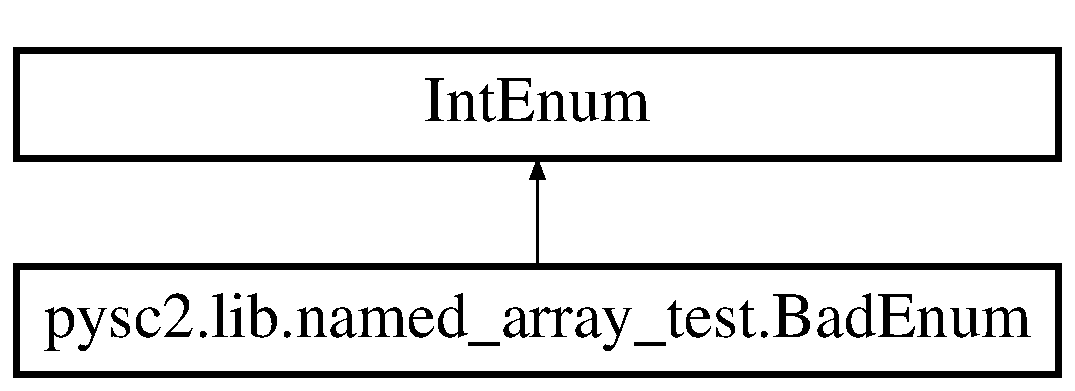
\includegraphics[height=2.000000cm]{classpysc2_1_1lib_1_1named__array__test_1_1_bad_enum}
\end{center}
\end{figure}
\subsection*{Static Public Attributes}
\begin{DoxyCompactItemize}
\item 
int \mbox{\hyperlink{classpysc2_1_1lib_1_1named__array__test_1_1_bad_enum_ac2011267dad627afd1b66d5974f69b4c}{a}} = 1
\item 
int \mbox{\hyperlink{classpysc2_1_1lib_1_1named__array__test_1_1_bad_enum_a39852f4bebf93c49f8043f731bf1990d}{b}} = 2
\item 
int \mbox{\hyperlink{classpysc2_1_1lib_1_1named__array__test_1_1_bad_enum_a08a980fdbdc2e50c68ccf8db768948f6}{c}} = 3
\end{DoxyCompactItemize}


\subsection{Member Data Documentation}
\mbox{\Hypertarget{classpysc2_1_1lib_1_1named__array__test_1_1_bad_enum_ac2011267dad627afd1b66d5974f69b4c}\label{classpysc2_1_1lib_1_1named__array__test_1_1_bad_enum_ac2011267dad627afd1b66d5974f69b4c}} 
\index{pysc2\+::lib\+::named\+\_\+array\+\_\+test\+::\+Bad\+Enum@{pysc2\+::lib\+::named\+\_\+array\+\_\+test\+::\+Bad\+Enum}!a@{a}}
\index{a@{a}!pysc2\+::lib\+::named\+\_\+array\+\_\+test\+::\+Bad\+Enum@{pysc2\+::lib\+::named\+\_\+array\+\_\+test\+::\+Bad\+Enum}}
\subsubsection{\texorpdfstring{a}{a}}
{\footnotesize\ttfamily int pysc2.\+lib.\+named\+\_\+array\+\_\+test.\+Bad\+Enum.\+a = 1\hspace{0.3cm}{\ttfamily [static]}}

\mbox{\Hypertarget{classpysc2_1_1lib_1_1named__array__test_1_1_bad_enum_a39852f4bebf93c49f8043f731bf1990d}\label{classpysc2_1_1lib_1_1named__array__test_1_1_bad_enum_a39852f4bebf93c49f8043f731bf1990d}} 
\index{pysc2\+::lib\+::named\+\_\+array\+\_\+test\+::\+Bad\+Enum@{pysc2\+::lib\+::named\+\_\+array\+\_\+test\+::\+Bad\+Enum}!b@{b}}
\index{b@{b}!pysc2\+::lib\+::named\+\_\+array\+\_\+test\+::\+Bad\+Enum@{pysc2\+::lib\+::named\+\_\+array\+\_\+test\+::\+Bad\+Enum}}
\subsubsection{\texorpdfstring{b}{b}}
{\footnotesize\ttfamily int pysc2.\+lib.\+named\+\_\+array\+\_\+test.\+Bad\+Enum.\+b = 2\hspace{0.3cm}{\ttfamily [static]}}

\mbox{\Hypertarget{classpysc2_1_1lib_1_1named__array__test_1_1_bad_enum_a08a980fdbdc2e50c68ccf8db768948f6}\label{classpysc2_1_1lib_1_1named__array__test_1_1_bad_enum_a08a980fdbdc2e50c68ccf8db768948f6}} 
\index{pysc2\+::lib\+::named\+\_\+array\+\_\+test\+::\+Bad\+Enum@{pysc2\+::lib\+::named\+\_\+array\+\_\+test\+::\+Bad\+Enum}!c@{c}}
\index{c@{c}!pysc2\+::lib\+::named\+\_\+array\+\_\+test\+::\+Bad\+Enum@{pysc2\+::lib\+::named\+\_\+array\+\_\+test\+::\+Bad\+Enum}}
\subsubsection{\texorpdfstring{c}{c}}
{\footnotesize\ttfamily int pysc2.\+lib.\+named\+\_\+array\+\_\+test.\+Bad\+Enum.\+c = 3\hspace{0.3cm}{\ttfamily [static]}}



The documentation for this class was generated from the following file\+:\begin{DoxyCompactItemize}
\item 
lib/\mbox{\hyperlink{named__array__test_8py}{named\+\_\+array\+\_\+test.\+py}}\end{DoxyCompactItemize}

\hypertarget{classpysc2_1_1lib_1_1named__array__test_1_1_bad_named_tuple}{}\section{pysc2.\+lib.\+named\+\_\+array\+\_\+test.\+Bad\+Named\+Tuple Class Reference}
\label{classpysc2_1_1lib_1_1named__array__test_1_1_bad_named_tuple}\index{pysc2.\+lib.\+named\+\_\+array\+\_\+test.\+Bad\+Named\+Tuple@{pysc2.\+lib.\+named\+\_\+array\+\_\+test.\+Bad\+Named\+Tuple}}
Inheritance diagram for pysc2.\+lib.\+named\+\_\+array\+\_\+test.\+Bad\+Named\+Tuple\+:\begin{figure}[H]
\begin{center}
\leavevmode
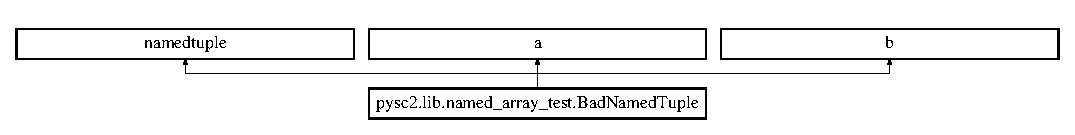
\includegraphics[height=1.372549cm]{classpysc2_1_1lib_1_1named__array__test_1_1_bad_named_tuple}
\end{center}
\end{figure}


The documentation for this class was generated from the following file\+:\begin{DoxyCompactItemize}
\item 
lib/\mbox{\hyperlink{named__array__test_8py}{named\+\_\+array\+\_\+test.\+py}}\end{DoxyCompactItemize}

\hypertarget{classpysc2_1_1lib_1_1run__parallel__test_1_1_barrier}{}\section{pysc2.\+lib.\+run\+\_\+parallel\+\_\+test.\+Barrier Class Reference}
\label{classpysc2_1_1lib_1_1run__parallel__test_1_1_barrier}\index{pysc2.\+lib.\+run\+\_\+parallel\+\_\+test.\+Barrier@{pysc2.\+lib.\+run\+\_\+parallel\+\_\+test.\+Barrier}}
Inheritance diagram for pysc2.\+lib.\+run\+\_\+parallel\+\_\+test.\+Barrier\+:\begin{figure}[H]
\begin{center}
\leavevmode
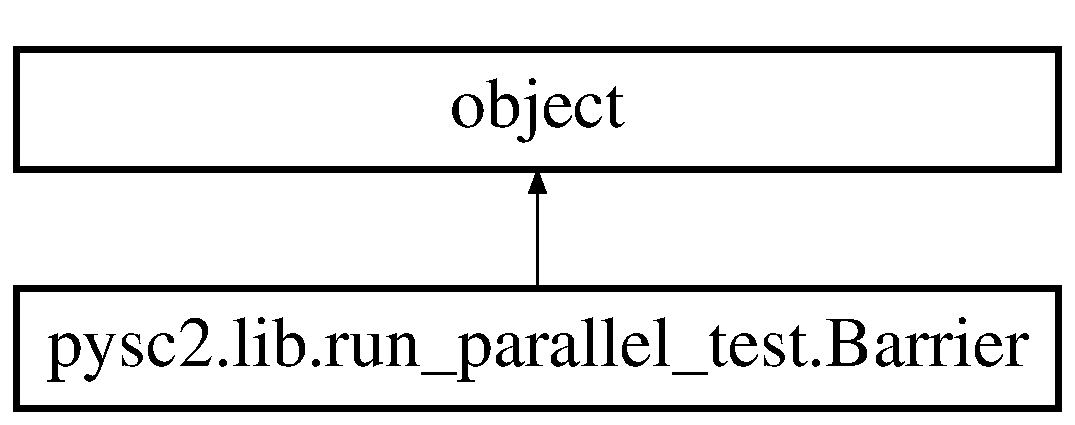
\includegraphics[height=2.000000cm]{classpysc2_1_1lib_1_1run__parallel__test_1_1_barrier}
\end{center}
\end{figure}
\subsection*{Public Member Functions}
\begin{DoxyCompactItemize}
\item 
def \mbox{\hyperlink{classpysc2_1_1lib_1_1run__parallel__test_1_1_barrier_a77e987f83cb0038718cddacc812e063c}{\+\_\+\+\_\+init\+\_\+\+\_\+}} (self, \mbox{\hyperlink{classpysc2_1_1lib_1_1run__parallel__test_1_1_barrier_ac8c9432b90c8b37ec7e5f0b5db77a473}{n}})
\item 
def \mbox{\hyperlink{classpysc2_1_1lib_1_1run__parallel__test_1_1_barrier_a0d5f345a8b99d03145c5c742e0f197f7}{wait}} (self)
\item 
def \mbox{\hyperlink{classpysc2_1_1lib_1_1run__parallel__test_1_1_barrier_a5216f6a490702f42fcead15daf544589}{clear}} (self)
\end{DoxyCompactItemize}
\subsection*{Public Attributes}
\begin{DoxyCompactItemize}
\item 
\mbox{\hyperlink{classpysc2_1_1lib_1_1run__parallel__test_1_1_barrier_ac8c9432b90c8b37ec7e5f0b5db77a473}{n}}
\item 
\mbox{\hyperlink{classpysc2_1_1lib_1_1run__parallel__test_1_1_barrier_aa4e9eeac4fac8f01df640fb2b881bf6d}{count}}
\item 
\mbox{\hyperlink{classpysc2_1_1lib_1_1run__parallel__test_1_1_barrier_a0439c79d387511bcea1606fea651388e}{cond}}
\end{DoxyCompactItemize}


\subsection{Constructor \& Destructor Documentation}
\mbox{\Hypertarget{classpysc2_1_1lib_1_1run__parallel__test_1_1_barrier_a77e987f83cb0038718cddacc812e063c}\label{classpysc2_1_1lib_1_1run__parallel__test_1_1_barrier_a77e987f83cb0038718cddacc812e063c}} 
\index{pysc2\+::lib\+::run\+\_\+parallel\+\_\+test\+::\+Barrier@{pysc2\+::lib\+::run\+\_\+parallel\+\_\+test\+::\+Barrier}!\+\_\+\+\_\+init\+\_\+\+\_\+@{\+\_\+\+\_\+init\+\_\+\+\_\+}}
\index{\+\_\+\+\_\+init\+\_\+\+\_\+@{\+\_\+\+\_\+init\+\_\+\+\_\+}!pysc2\+::lib\+::run\+\_\+parallel\+\_\+test\+::\+Barrier@{pysc2\+::lib\+::run\+\_\+parallel\+\_\+test\+::\+Barrier}}
\subsubsection{\texorpdfstring{\+\_\+\+\_\+init\+\_\+\+\_\+()}{\_\_init\_\_()}}
{\footnotesize\ttfamily def pysc2.\+lib.\+run\+\_\+parallel\+\_\+test.\+Barrier.\+\_\+\+\_\+init\+\_\+\+\_\+ (\begin{DoxyParamCaption}\item[{}]{self,  }\item[{}]{n }\end{DoxyParamCaption})}



\subsection{Member Function Documentation}
\mbox{\Hypertarget{classpysc2_1_1lib_1_1run__parallel__test_1_1_barrier_a5216f6a490702f42fcead15daf544589}\label{classpysc2_1_1lib_1_1run__parallel__test_1_1_barrier_a5216f6a490702f42fcead15daf544589}} 
\index{pysc2\+::lib\+::run\+\_\+parallel\+\_\+test\+::\+Barrier@{pysc2\+::lib\+::run\+\_\+parallel\+\_\+test\+::\+Barrier}!clear@{clear}}
\index{clear@{clear}!pysc2\+::lib\+::run\+\_\+parallel\+\_\+test\+::\+Barrier@{pysc2\+::lib\+::run\+\_\+parallel\+\_\+test\+::\+Barrier}}
\subsubsection{\texorpdfstring{clear()}{clear()}}
{\footnotesize\ttfamily def pysc2.\+lib.\+run\+\_\+parallel\+\_\+test.\+Barrier.\+clear (\begin{DoxyParamCaption}\item[{}]{self }\end{DoxyParamCaption})}

\mbox{\Hypertarget{classpysc2_1_1lib_1_1run__parallel__test_1_1_barrier_a0d5f345a8b99d03145c5c742e0f197f7}\label{classpysc2_1_1lib_1_1run__parallel__test_1_1_barrier_a0d5f345a8b99d03145c5c742e0f197f7}} 
\index{pysc2\+::lib\+::run\+\_\+parallel\+\_\+test\+::\+Barrier@{pysc2\+::lib\+::run\+\_\+parallel\+\_\+test\+::\+Barrier}!wait@{wait}}
\index{wait@{wait}!pysc2\+::lib\+::run\+\_\+parallel\+\_\+test\+::\+Barrier@{pysc2\+::lib\+::run\+\_\+parallel\+\_\+test\+::\+Barrier}}
\subsubsection{\texorpdfstring{wait()}{wait()}}
{\footnotesize\ttfamily def pysc2.\+lib.\+run\+\_\+parallel\+\_\+test.\+Barrier.\+wait (\begin{DoxyParamCaption}\item[{}]{self }\end{DoxyParamCaption})}



\subsection{Member Data Documentation}
\mbox{\Hypertarget{classpysc2_1_1lib_1_1run__parallel__test_1_1_barrier_a0439c79d387511bcea1606fea651388e}\label{classpysc2_1_1lib_1_1run__parallel__test_1_1_barrier_a0439c79d387511bcea1606fea651388e}} 
\index{pysc2\+::lib\+::run\+\_\+parallel\+\_\+test\+::\+Barrier@{pysc2\+::lib\+::run\+\_\+parallel\+\_\+test\+::\+Barrier}!cond@{cond}}
\index{cond@{cond}!pysc2\+::lib\+::run\+\_\+parallel\+\_\+test\+::\+Barrier@{pysc2\+::lib\+::run\+\_\+parallel\+\_\+test\+::\+Barrier}}
\subsubsection{\texorpdfstring{cond}{cond}}
{\footnotesize\ttfamily pysc2.\+lib.\+run\+\_\+parallel\+\_\+test.\+Barrier.\+cond}

\mbox{\Hypertarget{classpysc2_1_1lib_1_1run__parallel__test_1_1_barrier_aa4e9eeac4fac8f01df640fb2b881bf6d}\label{classpysc2_1_1lib_1_1run__parallel__test_1_1_barrier_aa4e9eeac4fac8f01df640fb2b881bf6d}} 
\index{pysc2\+::lib\+::run\+\_\+parallel\+\_\+test\+::\+Barrier@{pysc2\+::lib\+::run\+\_\+parallel\+\_\+test\+::\+Barrier}!count@{count}}
\index{count@{count}!pysc2\+::lib\+::run\+\_\+parallel\+\_\+test\+::\+Barrier@{pysc2\+::lib\+::run\+\_\+parallel\+\_\+test\+::\+Barrier}}
\subsubsection{\texorpdfstring{count}{count}}
{\footnotesize\ttfamily pysc2.\+lib.\+run\+\_\+parallel\+\_\+test.\+Barrier.\+count}

\mbox{\Hypertarget{classpysc2_1_1lib_1_1run__parallel__test_1_1_barrier_ac8c9432b90c8b37ec7e5f0b5db77a473}\label{classpysc2_1_1lib_1_1run__parallel__test_1_1_barrier_ac8c9432b90c8b37ec7e5f0b5db77a473}} 
\index{pysc2\+::lib\+::run\+\_\+parallel\+\_\+test\+::\+Barrier@{pysc2\+::lib\+::run\+\_\+parallel\+\_\+test\+::\+Barrier}!n@{n}}
\index{n@{n}!pysc2\+::lib\+::run\+\_\+parallel\+\_\+test\+::\+Barrier@{pysc2\+::lib\+::run\+\_\+parallel\+\_\+test\+::\+Barrier}}
\subsubsection{\texorpdfstring{n}{n}}
{\footnotesize\ttfamily pysc2.\+lib.\+run\+\_\+parallel\+\_\+test.\+Barrier.\+n}



The documentation for this class was generated from the following file\+:\begin{DoxyCompactItemize}
\item 
lib/\mbox{\hyperlink{run__parallel__test_8py}{run\+\_\+parallel\+\_\+test.\+py}}\end{DoxyCompactItemize}

\hypertarget{classpysc2_1_1env_1_1environment_1_1_base}{}\section{pysc2.\+env.\+environment.\+Base Class Reference}
\label{classpysc2_1_1env_1_1environment_1_1_base}\index{pysc2.\+env.\+environment.\+Base@{pysc2.\+env.\+environment.\+Base}}
Inheritance diagram for pysc2.\+env.\+environment.\+Base\+:\begin{figure}[H]
\begin{center}
\leavevmode
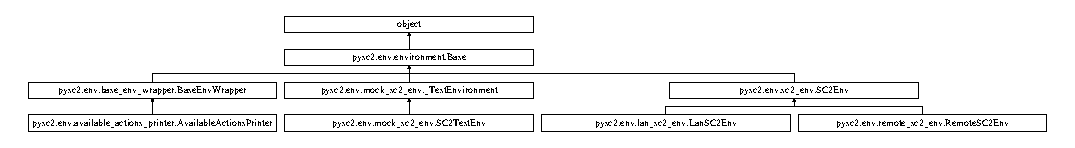
\includegraphics[height=1.546961cm]{classpysc2_1_1env_1_1environment_1_1_base}
\end{center}
\end{figure}


The documentation for this class was generated from the following file\+:\begin{DoxyCompactItemize}
\item 
env/\mbox{\hyperlink{environment_8py}{environment.\+py}}\end{DoxyCompactItemize}

\hypertarget{classpysc2_1_1agents_1_1base__agent_1_1_base_agent}{}\section{pysc2.\+agents.\+base\+\_\+agent.\+Base\+Agent Class Reference}
\label{classpysc2_1_1agents_1_1base__agent_1_1_base_agent}\index{pysc2.\+agents.\+base\+\_\+agent.\+Base\+Agent@{pysc2.\+agents.\+base\+\_\+agent.\+Base\+Agent}}
Inheritance diagram for pysc2.\+agents.\+base\+\_\+agent.\+Base\+Agent\+:\begin{figure}[H]
\begin{center}
\leavevmode
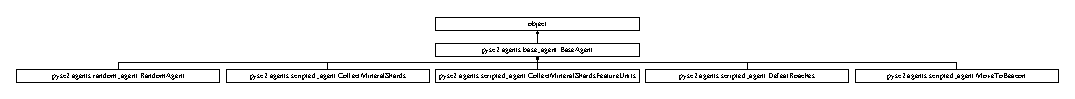
\includegraphics[height=0.886544cm]{classpysc2_1_1agents_1_1base__agent_1_1_base_agent}
\end{center}
\end{figure}
\subsection*{Public Member Functions}
\begin{DoxyCompactItemize}
\item 
def \mbox{\hyperlink{classpysc2_1_1agents_1_1base__agent_1_1_base_agent_a03935d754145f417240d25e0192c57bc}{\+\_\+\+\_\+init\+\_\+\+\_\+}} (self)
\item 
def \mbox{\hyperlink{classpysc2_1_1agents_1_1base__agent_1_1_base_agent_afba8f06273c8740b105573f1a422ba05}{setup}} (self, \mbox{\hyperlink{classpysc2_1_1agents_1_1base__agent_1_1_base_agent_ad6cefb81724b9d234887cea543c4f06e}{obs\+\_\+spec}}, \mbox{\hyperlink{classpysc2_1_1agents_1_1base__agent_1_1_base_agent_a550b216b98ae40b2da1b2fd9015d3019}{action\+\_\+spec}})
\item 
def \mbox{\hyperlink{classpysc2_1_1agents_1_1base__agent_1_1_base_agent_a9814c84f6f2eefa13b69f45f36afcca4}{reset}} (self)
\item 
def \mbox{\hyperlink{classpysc2_1_1agents_1_1base__agent_1_1_base_agent_a64b82c5e648902378e9485b27be6dc0b}{step}} (self, obs)
\end{DoxyCompactItemize}
\subsection*{Public Attributes}
\begin{DoxyCompactItemize}
\item 
\mbox{\hyperlink{classpysc2_1_1agents_1_1base__agent_1_1_base_agent_a9081eba1a1a529a08d1309e35a1f7ad9}{reward}}
\item 
\mbox{\hyperlink{classpysc2_1_1agents_1_1base__agent_1_1_base_agent_a46c85c12c80d0ceceff90c5889f0a13a}{episodes}}
\item 
\mbox{\hyperlink{classpysc2_1_1agents_1_1base__agent_1_1_base_agent_aac3b906e1bc4bfc1fad84e8a1fb6ef87}{steps}}
\item 
\mbox{\hyperlink{classpysc2_1_1agents_1_1base__agent_1_1_base_agent_ad6cefb81724b9d234887cea543c4f06e}{obs\+\_\+spec}}
\item 
\mbox{\hyperlink{classpysc2_1_1agents_1_1base__agent_1_1_base_agent_a550b216b98ae40b2da1b2fd9015d3019}{action\+\_\+spec}}
\end{DoxyCompactItemize}


\subsection{Detailed Description}
\begin{DoxyVerb}A base agent to write custom scripted agents.

It can also act as a passive agent that does nothing but no-ops.
\end{DoxyVerb}
 

\subsection{Constructor \& Destructor Documentation}
\mbox{\Hypertarget{classpysc2_1_1agents_1_1base__agent_1_1_base_agent_a03935d754145f417240d25e0192c57bc}\label{classpysc2_1_1agents_1_1base__agent_1_1_base_agent_a03935d754145f417240d25e0192c57bc}} 
\index{pysc2\+::agents\+::base\+\_\+agent\+::\+Base\+Agent@{pysc2\+::agents\+::base\+\_\+agent\+::\+Base\+Agent}!\+\_\+\+\_\+init\+\_\+\+\_\+@{\+\_\+\+\_\+init\+\_\+\+\_\+}}
\index{\+\_\+\+\_\+init\+\_\+\+\_\+@{\+\_\+\+\_\+init\+\_\+\+\_\+}!pysc2\+::agents\+::base\+\_\+agent\+::\+Base\+Agent@{pysc2\+::agents\+::base\+\_\+agent\+::\+Base\+Agent}}
\subsubsection{\texorpdfstring{\+\_\+\+\_\+init\+\_\+\+\_\+()}{\_\_init\_\_()}}
{\footnotesize\ttfamily def pysc2.\+agents.\+base\+\_\+agent.\+Base\+Agent.\+\_\+\+\_\+init\+\_\+\+\_\+ (\begin{DoxyParamCaption}\item[{}]{self }\end{DoxyParamCaption})}



\subsection{Member Function Documentation}
\mbox{\Hypertarget{classpysc2_1_1agents_1_1base__agent_1_1_base_agent_a9814c84f6f2eefa13b69f45f36afcca4}\label{classpysc2_1_1agents_1_1base__agent_1_1_base_agent_a9814c84f6f2eefa13b69f45f36afcca4}} 
\index{pysc2\+::agents\+::base\+\_\+agent\+::\+Base\+Agent@{pysc2\+::agents\+::base\+\_\+agent\+::\+Base\+Agent}!reset@{reset}}
\index{reset@{reset}!pysc2\+::agents\+::base\+\_\+agent\+::\+Base\+Agent@{pysc2\+::agents\+::base\+\_\+agent\+::\+Base\+Agent}}
\subsubsection{\texorpdfstring{reset()}{reset()}}
{\footnotesize\ttfamily def pysc2.\+agents.\+base\+\_\+agent.\+Base\+Agent.\+reset (\begin{DoxyParamCaption}\item[{}]{self }\end{DoxyParamCaption})}

\mbox{\Hypertarget{classpysc2_1_1agents_1_1base__agent_1_1_base_agent_afba8f06273c8740b105573f1a422ba05}\label{classpysc2_1_1agents_1_1base__agent_1_1_base_agent_afba8f06273c8740b105573f1a422ba05}} 
\index{pysc2\+::agents\+::base\+\_\+agent\+::\+Base\+Agent@{pysc2\+::agents\+::base\+\_\+agent\+::\+Base\+Agent}!setup@{setup}}
\index{setup@{setup}!pysc2\+::agents\+::base\+\_\+agent\+::\+Base\+Agent@{pysc2\+::agents\+::base\+\_\+agent\+::\+Base\+Agent}}
\subsubsection{\texorpdfstring{setup()}{setup()}}
{\footnotesize\ttfamily def pysc2.\+agents.\+base\+\_\+agent.\+Base\+Agent.\+setup (\begin{DoxyParamCaption}\item[{}]{self,  }\item[{}]{obs\+\_\+spec,  }\item[{}]{action\+\_\+spec }\end{DoxyParamCaption})}

\mbox{\Hypertarget{classpysc2_1_1agents_1_1base__agent_1_1_base_agent_a64b82c5e648902378e9485b27be6dc0b}\label{classpysc2_1_1agents_1_1base__agent_1_1_base_agent_a64b82c5e648902378e9485b27be6dc0b}} 
\index{pysc2\+::agents\+::base\+\_\+agent\+::\+Base\+Agent@{pysc2\+::agents\+::base\+\_\+agent\+::\+Base\+Agent}!step@{step}}
\index{step@{step}!pysc2\+::agents\+::base\+\_\+agent\+::\+Base\+Agent@{pysc2\+::agents\+::base\+\_\+agent\+::\+Base\+Agent}}
\subsubsection{\texorpdfstring{step()}{step()}}
{\footnotesize\ttfamily def pysc2.\+agents.\+base\+\_\+agent.\+Base\+Agent.\+step (\begin{DoxyParamCaption}\item[{}]{self,  }\item[{}]{obs }\end{DoxyParamCaption})}



\subsection{Member Data Documentation}
\mbox{\Hypertarget{classpysc2_1_1agents_1_1base__agent_1_1_base_agent_a550b216b98ae40b2da1b2fd9015d3019}\label{classpysc2_1_1agents_1_1base__agent_1_1_base_agent_a550b216b98ae40b2da1b2fd9015d3019}} 
\index{pysc2\+::agents\+::base\+\_\+agent\+::\+Base\+Agent@{pysc2\+::agents\+::base\+\_\+agent\+::\+Base\+Agent}!action\+\_\+spec@{action\+\_\+spec}}
\index{action\+\_\+spec@{action\+\_\+spec}!pysc2\+::agents\+::base\+\_\+agent\+::\+Base\+Agent@{pysc2\+::agents\+::base\+\_\+agent\+::\+Base\+Agent}}
\subsubsection{\texorpdfstring{action\+\_\+spec}{action\_spec}}
{\footnotesize\ttfamily pysc2.\+agents.\+base\+\_\+agent.\+Base\+Agent.\+action\+\_\+spec}

\mbox{\Hypertarget{classpysc2_1_1agents_1_1base__agent_1_1_base_agent_a46c85c12c80d0ceceff90c5889f0a13a}\label{classpysc2_1_1agents_1_1base__agent_1_1_base_agent_a46c85c12c80d0ceceff90c5889f0a13a}} 
\index{pysc2\+::agents\+::base\+\_\+agent\+::\+Base\+Agent@{pysc2\+::agents\+::base\+\_\+agent\+::\+Base\+Agent}!episodes@{episodes}}
\index{episodes@{episodes}!pysc2\+::agents\+::base\+\_\+agent\+::\+Base\+Agent@{pysc2\+::agents\+::base\+\_\+agent\+::\+Base\+Agent}}
\subsubsection{\texorpdfstring{episodes}{episodes}}
{\footnotesize\ttfamily pysc2.\+agents.\+base\+\_\+agent.\+Base\+Agent.\+episodes}

\mbox{\Hypertarget{classpysc2_1_1agents_1_1base__agent_1_1_base_agent_ad6cefb81724b9d234887cea543c4f06e}\label{classpysc2_1_1agents_1_1base__agent_1_1_base_agent_ad6cefb81724b9d234887cea543c4f06e}} 
\index{pysc2\+::agents\+::base\+\_\+agent\+::\+Base\+Agent@{pysc2\+::agents\+::base\+\_\+agent\+::\+Base\+Agent}!obs\+\_\+spec@{obs\+\_\+spec}}
\index{obs\+\_\+spec@{obs\+\_\+spec}!pysc2\+::agents\+::base\+\_\+agent\+::\+Base\+Agent@{pysc2\+::agents\+::base\+\_\+agent\+::\+Base\+Agent}}
\subsubsection{\texorpdfstring{obs\+\_\+spec}{obs\_spec}}
{\footnotesize\ttfamily pysc2.\+agents.\+base\+\_\+agent.\+Base\+Agent.\+obs\+\_\+spec}

\mbox{\Hypertarget{classpysc2_1_1agents_1_1base__agent_1_1_base_agent_a9081eba1a1a529a08d1309e35a1f7ad9}\label{classpysc2_1_1agents_1_1base__agent_1_1_base_agent_a9081eba1a1a529a08d1309e35a1f7ad9}} 
\index{pysc2\+::agents\+::base\+\_\+agent\+::\+Base\+Agent@{pysc2\+::agents\+::base\+\_\+agent\+::\+Base\+Agent}!reward@{reward}}
\index{reward@{reward}!pysc2\+::agents\+::base\+\_\+agent\+::\+Base\+Agent@{pysc2\+::agents\+::base\+\_\+agent\+::\+Base\+Agent}}
\subsubsection{\texorpdfstring{reward}{reward}}
{\footnotesize\ttfamily pysc2.\+agents.\+base\+\_\+agent.\+Base\+Agent.\+reward}

\mbox{\Hypertarget{classpysc2_1_1agents_1_1base__agent_1_1_base_agent_aac3b906e1bc4bfc1fad84e8a1fb6ef87}\label{classpysc2_1_1agents_1_1base__agent_1_1_base_agent_aac3b906e1bc4bfc1fad84e8a1fb6ef87}} 
\index{pysc2\+::agents\+::base\+\_\+agent\+::\+Base\+Agent@{pysc2\+::agents\+::base\+\_\+agent\+::\+Base\+Agent}!steps@{steps}}
\index{steps@{steps}!pysc2\+::agents\+::base\+\_\+agent\+::\+Base\+Agent@{pysc2\+::agents\+::base\+\_\+agent\+::\+Base\+Agent}}
\subsubsection{\texorpdfstring{steps}{steps}}
{\footnotesize\ttfamily pysc2.\+agents.\+base\+\_\+agent.\+Base\+Agent.\+steps}



The documentation for this class was generated from the following file\+:\begin{DoxyCompactItemize}
\item 
agents/\mbox{\hyperlink{base__agent_8py}{base\+\_\+agent.\+py}}\end{DoxyCompactItemize}

\hypertarget{classpysc2_1_1env_1_1base__env__wrapper_1_1_base_env_wrapper}{}\section{pysc2.\+env.\+base\+\_\+env\+\_\+wrapper.\+Base\+Env\+Wrapper Class Reference}
\label{classpysc2_1_1env_1_1base__env__wrapper_1_1_base_env_wrapper}\index{pysc2.\+env.\+base\+\_\+env\+\_\+wrapper.\+Base\+Env\+Wrapper@{pysc2.\+env.\+base\+\_\+env\+\_\+wrapper.\+Base\+Env\+Wrapper}}
Inheritance diagram for pysc2.\+env.\+base\+\_\+env\+\_\+wrapper.\+Base\+Env\+Wrapper\+:\begin{figure}[H]
\begin{center}
\leavevmode
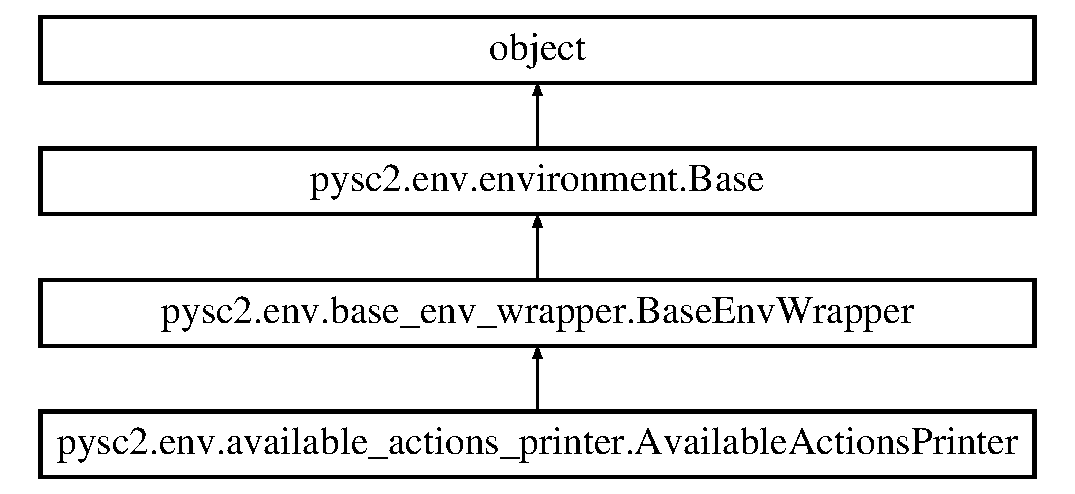
\includegraphics[height=4.000000cm]{classpysc2_1_1env_1_1base__env__wrapper_1_1_base_env_wrapper}
\end{center}
\end{figure}
\subsection*{Public Member Functions}
\begin{DoxyCompactItemize}
\item 
def \mbox{\hyperlink{classpysc2_1_1env_1_1base__env__wrapper_1_1_base_env_wrapper_a559e7740680ee3bea19dad409eaba8e6}{\+\_\+\+\_\+init\+\_\+\+\_\+}} (self, env)
\item 
def \mbox{\hyperlink{classpysc2_1_1env_1_1base__env__wrapper_1_1_base_env_wrapper_a7c67bf47a58d4ca0857fbca0664842b0}{close}} (self, args, kwargs)
\item 
def \mbox{\hyperlink{classpysc2_1_1env_1_1base__env__wrapper_1_1_base_env_wrapper_aceb8c9f065aac5de979d8b9fe2dde82b}{action\+\_\+spec}} (self, args, kwargs)
\item 
def \mbox{\hyperlink{classpysc2_1_1env_1_1base__env__wrapper_1_1_base_env_wrapper_a1b4fec660232a73e8985d96f77b30ec3}{observation\+\_\+spec}} (self, args, kwargs)
\item 
def \mbox{\hyperlink{classpysc2_1_1env_1_1base__env__wrapper_1_1_base_env_wrapper_a6b528f10880414b3adbf2d55cf25d48b}{reset}} (self, args, kwargs)
\item 
def \mbox{\hyperlink{classpysc2_1_1env_1_1base__env__wrapper_1_1_base_env_wrapper_ab491e6f3a60fb773ba3573ebbd49cfc5}{step}} (self, args, kwargs)
\item 
def \mbox{\hyperlink{classpysc2_1_1env_1_1base__env__wrapper_1_1_base_env_wrapper_a60cf932110b1a4ec35d36c719ae8b045}{save\+\_\+replay}} (self, args, kwargs)
\item 
def \mbox{\hyperlink{classpysc2_1_1env_1_1base__env__wrapper_1_1_base_env_wrapper_a8b4ada1faebd56dfdc44640b74078e91}{state}} (self)
\end{DoxyCompactItemize}


\subsection{Detailed Description}
\begin{DoxyVerb}A base env wrapper so we don't need to override everything every time.\end{DoxyVerb}
 

\subsection{Constructor \& Destructor Documentation}
\mbox{\Hypertarget{classpysc2_1_1env_1_1base__env__wrapper_1_1_base_env_wrapper_a559e7740680ee3bea19dad409eaba8e6}\label{classpysc2_1_1env_1_1base__env__wrapper_1_1_base_env_wrapper_a559e7740680ee3bea19dad409eaba8e6}} 
\index{pysc2\+::env\+::base\+\_\+env\+\_\+wrapper\+::\+Base\+Env\+Wrapper@{pysc2\+::env\+::base\+\_\+env\+\_\+wrapper\+::\+Base\+Env\+Wrapper}!\+\_\+\+\_\+init\+\_\+\+\_\+@{\+\_\+\+\_\+init\+\_\+\+\_\+}}
\index{\+\_\+\+\_\+init\+\_\+\+\_\+@{\+\_\+\+\_\+init\+\_\+\+\_\+}!pysc2\+::env\+::base\+\_\+env\+\_\+wrapper\+::\+Base\+Env\+Wrapper@{pysc2\+::env\+::base\+\_\+env\+\_\+wrapper\+::\+Base\+Env\+Wrapper}}
\subsubsection{\texorpdfstring{\+\_\+\+\_\+init\+\_\+\+\_\+()}{\_\_init\_\_()}}
{\footnotesize\ttfamily def pysc2.\+env.\+base\+\_\+env\+\_\+wrapper.\+Base\+Env\+Wrapper.\+\_\+\+\_\+init\+\_\+\+\_\+ (\begin{DoxyParamCaption}\item[{}]{self,  }\item[{}]{env }\end{DoxyParamCaption})}



\subsection{Member Function Documentation}
\mbox{\Hypertarget{classpysc2_1_1env_1_1base__env__wrapper_1_1_base_env_wrapper_aceb8c9f065aac5de979d8b9fe2dde82b}\label{classpysc2_1_1env_1_1base__env__wrapper_1_1_base_env_wrapper_aceb8c9f065aac5de979d8b9fe2dde82b}} 
\index{pysc2\+::env\+::base\+\_\+env\+\_\+wrapper\+::\+Base\+Env\+Wrapper@{pysc2\+::env\+::base\+\_\+env\+\_\+wrapper\+::\+Base\+Env\+Wrapper}!action\+\_\+spec@{action\+\_\+spec}}
\index{action\+\_\+spec@{action\+\_\+spec}!pysc2\+::env\+::base\+\_\+env\+\_\+wrapper\+::\+Base\+Env\+Wrapper@{pysc2\+::env\+::base\+\_\+env\+\_\+wrapper\+::\+Base\+Env\+Wrapper}}
\subsubsection{\texorpdfstring{action\+\_\+spec()}{action\_spec()}}
{\footnotesize\ttfamily def pysc2.\+env.\+base\+\_\+env\+\_\+wrapper.\+Base\+Env\+Wrapper.\+action\+\_\+spec (\begin{DoxyParamCaption}\item[{}]{self,  }\item[{}]{args,  }\item[{}]{kwargs }\end{DoxyParamCaption})}

\mbox{\Hypertarget{classpysc2_1_1env_1_1base__env__wrapper_1_1_base_env_wrapper_a7c67bf47a58d4ca0857fbca0664842b0}\label{classpysc2_1_1env_1_1base__env__wrapper_1_1_base_env_wrapper_a7c67bf47a58d4ca0857fbca0664842b0}} 
\index{pysc2\+::env\+::base\+\_\+env\+\_\+wrapper\+::\+Base\+Env\+Wrapper@{pysc2\+::env\+::base\+\_\+env\+\_\+wrapper\+::\+Base\+Env\+Wrapper}!close@{close}}
\index{close@{close}!pysc2\+::env\+::base\+\_\+env\+\_\+wrapper\+::\+Base\+Env\+Wrapper@{pysc2\+::env\+::base\+\_\+env\+\_\+wrapper\+::\+Base\+Env\+Wrapper}}
\subsubsection{\texorpdfstring{close()}{close()}}
{\footnotesize\ttfamily def pysc2.\+env.\+base\+\_\+env\+\_\+wrapper.\+Base\+Env\+Wrapper.\+close (\begin{DoxyParamCaption}\item[{}]{self,  }\item[{}]{args,  }\item[{}]{kwargs }\end{DoxyParamCaption})}

\mbox{\Hypertarget{classpysc2_1_1env_1_1base__env__wrapper_1_1_base_env_wrapper_a1b4fec660232a73e8985d96f77b30ec3}\label{classpysc2_1_1env_1_1base__env__wrapper_1_1_base_env_wrapper_a1b4fec660232a73e8985d96f77b30ec3}} 
\index{pysc2\+::env\+::base\+\_\+env\+\_\+wrapper\+::\+Base\+Env\+Wrapper@{pysc2\+::env\+::base\+\_\+env\+\_\+wrapper\+::\+Base\+Env\+Wrapper}!observation\+\_\+spec@{observation\+\_\+spec}}
\index{observation\+\_\+spec@{observation\+\_\+spec}!pysc2\+::env\+::base\+\_\+env\+\_\+wrapper\+::\+Base\+Env\+Wrapper@{pysc2\+::env\+::base\+\_\+env\+\_\+wrapper\+::\+Base\+Env\+Wrapper}}
\subsubsection{\texorpdfstring{observation\+\_\+spec()}{observation\_spec()}}
{\footnotesize\ttfamily def pysc2.\+env.\+base\+\_\+env\+\_\+wrapper.\+Base\+Env\+Wrapper.\+observation\+\_\+spec (\begin{DoxyParamCaption}\item[{}]{self,  }\item[{}]{args,  }\item[{}]{kwargs }\end{DoxyParamCaption})}

\mbox{\Hypertarget{classpysc2_1_1env_1_1base__env__wrapper_1_1_base_env_wrapper_a6b528f10880414b3adbf2d55cf25d48b}\label{classpysc2_1_1env_1_1base__env__wrapper_1_1_base_env_wrapper_a6b528f10880414b3adbf2d55cf25d48b}} 
\index{pysc2\+::env\+::base\+\_\+env\+\_\+wrapper\+::\+Base\+Env\+Wrapper@{pysc2\+::env\+::base\+\_\+env\+\_\+wrapper\+::\+Base\+Env\+Wrapper}!reset@{reset}}
\index{reset@{reset}!pysc2\+::env\+::base\+\_\+env\+\_\+wrapper\+::\+Base\+Env\+Wrapper@{pysc2\+::env\+::base\+\_\+env\+\_\+wrapper\+::\+Base\+Env\+Wrapper}}
\subsubsection{\texorpdfstring{reset()}{reset()}}
{\footnotesize\ttfamily def pysc2.\+env.\+base\+\_\+env\+\_\+wrapper.\+Base\+Env\+Wrapper.\+reset (\begin{DoxyParamCaption}\item[{}]{self,  }\item[{}]{args,  }\item[{}]{kwargs }\end{DoxyParamCaption})}

\mbox{\Hypertarget{classpysc2_1_1env_1_1base__env__wrapper_1_1_base_env_wrapper_a60cf932110b1a4ec35d36c719ae8b045}\label{classpysc2_1_1env_1_1base__env__wrapper_1_1_base_env_wrapper_a60cf932110b1a4ec35d36c719ae8b045}} 
\index{pysc2\+::env\+::base\+\_\+env\+\_\+wrapper\+::\+Base\+Env\+Wrapper@{pysc2\+::env\+::base\+\_\+env\+\_\+wrapper\+::\+Base\+Env\+Wrapper}!save\+\_\+replay@{save\+\_\+replay}}
\index{save\+\_\+replay@{save\+\_\+replay}!pysc2\+::env\+::base\+\_\+env\+\_\+wrapper\+::\+Base\+Env\+Wrapper@{pysc2\+::env\+::base\+\_\+env\+\_\+wrapper\+::\+Base\+Env\+Wrapper}}
\subsubsection{\texorpdfstring{save\+\_\+replay()}{save\_replay()}}
{\footnotesize\ttfamily def pysc2.\+env.\+base\+\_\+env\+\_\+wrapper.\+Base\+Env\+Wrapper.\+save\+\_\+replay (\begin{DoxyParamCaption}\item[{}]{self,  }\item[{}]{args,  }\item[{}]{kwargs }\end{DoxyParamCaption})}

\mbox{\Hypertarget{classpysc2_1_1env_1_1base__env__wrapper_1_1_base_env_wrapper_a8b4ada1faebd56dfdc44640b74078e91}\label{classpysc2_1_1env_1_1base__env__wrapper_1_1_base_env_wrapper_a8b4ada1faebd56dfdc44640b74078e91}} 
\index{pysc2\+::env\+::base\+\_\+env\+\_\+wrapper\+::\+Base\+Env\+Wrapper@{pysc2\+::env\+::base\+\_\+env\+\_\+wrapper\+::\+Base\+Env\+Wrapper}!state@{state}}
\index{state@{state}!pysc2\+::env\+::base\+\_\+env\+\_\+wrapper\+::\+Base\+Env\+Wrapper@{pysc2\+::env\+::base\+\_\+env\+\_\+wrapper\+::\+Base\+Env\+Wrapper}}
\subsubsection{\texorpdfstring{state()}{state()}}
{\footnotesize\ttfamily def pysc2.\+env.\+base\+\_\+env\+\_\+wrapper.\+Base\+Env\+Wrapper.\+state (\begin{DoxyParamCaption}\item[{}]{self }\end{DoxyParamCaption})}

\mbox{\Hypertarget{classpysc2_1_1env_1_1base__env__wrapper_1_1_base_env_wrapper_ab491e6f3a60fb773ba3573ebbd49cfc5}\label{classpysc2_1_1env_1_1base__env__wrapper_1_1_base_env_wrapper_ab491e6f3a60fb773ba3573ebbd49cfc5}} 
\index{pysc2\+::env\+::base\+\_\+env\+\_\+wrapper\+::\+Base\+Env\+Wrapper@{pysc2\+::env\+::base\+\_\+env\+\_\+wrapper\+::\+Base\+Env\+Wrapper}!step@{step}}
\index{step@{step}!pysc2\+::env\+::base\+\_\+env\+\_\+wrapper\+::\+Base\+Env\+Wrapper@{pysc2\+::env\+::base\+\_\+env\+\_\+wrapper\+::\+Base\+Env\+Wrapper}}
\subsubsection{\texorpdfstring{step()}{step()}}
{\footnotesize\ttfamily def pysc2.\+env.\+base\+\_\+env\+\_\+wrapper.\+Base\+Env\+Wrapper.\+step (\begin{DoxyParamCaption}\item[{}]{self,  }\item[{}]{args,  }\item[{}]{kwargs }\end{DoxyParamCaption})}



The documentation for this class was generated from the following file\+:\begin{DoxyCompactItemize}
\item 
env/\mbox{\hyperlink{base__env__wrapper_8py}{base\+\_\+env\+\_\+wrapper.\+py}}\end{DoxyCompactItemize}

\hypertarget{classpysc2_1_1tests_1_1dummy__observation_1_1_builder}{}\section{pysc2.\+tests.\+dummy\+\_\+observation.\+Builder Class Reference}
\label{classpysc2_1_1tests_1_1dummy__observation_1_1_builder}\index{pysc2.\+tests.\+dummy\+\_\+observation.\+Builder@{pysc2.\+tests.\+dummy\+\_\+observation.\+Builder}}
Inheritance diagram for pysc2.\+tests.\+dummy\+\_\+observation.\+Builder\+:\begin{figure}[H]
\begin{center}
\leavevmode
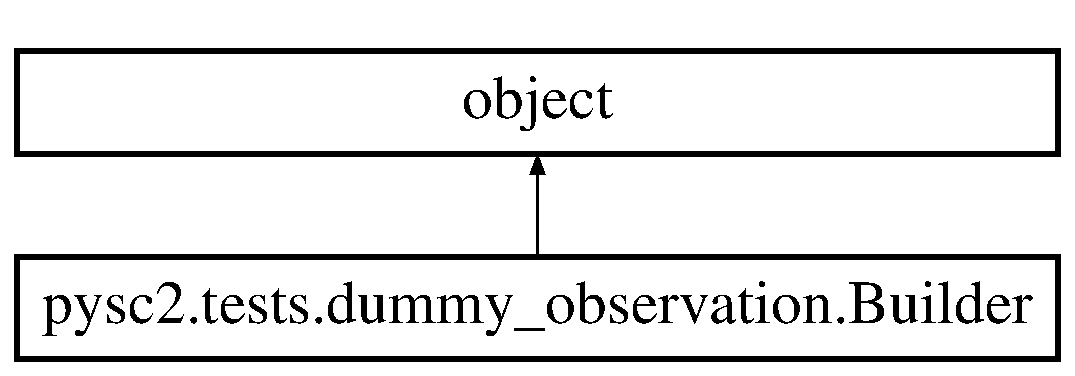
\includegraphics[height=2.000000cm]{classpysc2_1_1tests_1_1dummy__observation_1_1_builder}
\end{center}
\end{figure}
\subsection*{Public Member Functions}
\begin{DoxyCompactItemize}
\item 
def \mbox{\hyperlink{classpysc2_1_1tests_1_1dummy__observation_1_1_builder_a6605dc28807b3a5ecf40cbbb1f4efe49}{\+\_\+\+\_\+init\+\_\+\+\_\+}} (self, obs\+\_\+spec)
\item 
def \mbox{\hyperlink{classpysc2_1_1tests_1_1dummy__observation_1_1_builder_abc12bdd5824b2fb1c4ad73f49d9a24c2}{single\+\_\+select}} (self, unit)
\item 
def \mbox{\hyperlink{classpysc2_1_1tests_1_1dummy__observation_1_1_builder_abd244158d236d9f802b95119b8aca326}{multi\+\_\+select}} (self, units)
\item 
def \mbox{\hyperlink{classpysc2_1_1tests_1_1dummy__observation_1_1_builder_aa93d367215f3fdc8aa7adae07999577a}{feature\+\_\+units}} (self, feature\+\_\+units)
\item 
def \mbox{\hyperlink{classpysc2_1_1tests_1_1dummy__observation_1_1_builder_ab74de5b9e8e2073e12b5712a90cea67d}{build}} (self)
\end{DoxyCompactItemize}


\subsection{Detailed Description}
\begin{DoxyVerb}For test code - build a dummy ResponseObservation proto.\end{DoxyVerb}
 

\subsection{Constructor \& Destructor Documentation}
\mbox{\Hypertarget{classpysc2_1_1tests_1_1dummy__observation_1_1_builder_a6605dc28807b3a5ecf40cbbb1f4efe49}\label{classpysc2_1_1tests_1_1dummy__observation_1_1_builder_a6605dc28807b3a5ecf40cbbb1f4efe49}} 
\index{pysc2\+::tests\+::dummy\+\_\+observation\+::\+Builder@{pysc2\+::tests\+::dummy\+\_\+observation\+::\+Builder}!\+\_\+\+\_\+init\+\_\+\+\_\+@{\+\_\+\+\_\+init\+\_\+\+\_\+}}
\index{\+\_\+\+\_\+init\+\_\+\+\_\+@{\+\_\+\+\_\+init\+\_\+\+\_\+}!pysc2\+::tests\+::dummy\+\_\+observation\+::\+Builder@{pysc2\+::tests\+::dummy\+\_\+observation\+::\+Builder}}
\subsubsection{\texorpdfstring{\+\_\+\+\_\+init\+\_\+\+\_\+()}{\_\_init\_\_()}}
{\footnotesize\ttfamily def pysc2.\+tests.\+dummy\+\_\+observation.\+Builder.\+\_\+\+\_\+init\+\_\+\+\_\+ (\begin{DoxyParamCaption}\item[{}]{self,  }\item[{}]{obs\+\_\+spec }\end{DoxyParamCaption})}



\subsection{Member Function Documentation}
\mbox{\Hypertarget{classpysc2_1_1tests_1_1dummy__observation_1_1_builder_ab74de5b9e8e2073e12b5712a90cea67d}\label{classpysc2_1_1tests_1_1dummy__observation_1_1_builder_ab74de5b9e8e2073e12b5712a90cea67d}} 
\index{pysc2\+::tests\+::dummy\+\_\+observation\+::\+Builder@{pysc2\+::tests\+::dummy\+\_\+observation\+::\+Builder}!build@{build}}
\index{build@{build}!pysc2\+::tests\+::dummy\+\_\+observation\+::\+Builder@{pysc2\+::tests\+::dummy\+\_\+observation\+::\+Builder}}
\subsubsection{\texorpdfstring{build()}{build()}}
{\footnotesize\ttfamily def pysc2.\+tests.\+dummy\+\_\+observation.\+Builder.\+build (\begin{DoxyParamCaption}\item[{}]{self }\end{DoxyParamCaption})}

\begin{DoxyVerb}Builds and returns a proto ResponseObservation.\end{DoxyVerb}
 \mbox{\Hypertarget{classpysc2_1_1tests_1_1dummy__observation_1_1_builder_aa93d367215f3fdc8aa7adae07999577a}\label{classpysc2_1_1tests_1_1dummy__observation_1_1_builder_aa93d367215f3fdc8aa7adae07999577a}} 
\index{pysc2\+::tests\+::dummy\+\_\+observation\+::\+Builder@{pysc2\+::tests\+::dummy\+\_\+observation\+::\+Builder}!feature\+\_\+units@{feature\+\_\+units}}
\index{feature\+\_\+units@{feature\+\_\+units}!pysc2\+::tests\+::dummy\+\_\+observation\+::\+Builder@{pysc2\+::tests\+::dummy\+\_\+observation\+::\+Builder}}
\subsubsection{\texorpdfstring{feature\+\_\+units()}{feature\_units()}}
{\footnotesize\ttfamily def pysc2.\+tests.\+dummy\+\_\+observation.\+Builder.\+feature\+\_\+units (\begin{DoxyParamCaption}\item[{}]{self,  }\item[{}]{feature\+\_\+units }\end{DoxyParamCaption})}

\mbox{\Hypertarget{classpysc2_1_1tests_1_1dummy__observation_1_1_builder_abd244158d236d9f802b95119b8aca326}\label{classpysc2_1_1tests_1_1dummy__observation_1_1_builder_abd244158d236d9f802b95119b8aca326}} 
\index{pysc2\+::tests\+::dummy\+\_\+observation\+::\+Builder@{pysc2\+::tests\+::dummy\+\_\+observation\+::\+Builder}!multi\+\_\+select@{multi\+\_\+select}}
\index{multi\+\_\+select@{multi\+\_\+select}!pysc2\+::tests\+::dummy\+\_\+observation\+::\+Builder@{pysc2\+::tests\+::dummy\+\_\+observation\+::\+Builder}}
\subsubsection{\texorpdfstring{multi\+\_\+select()}{multi\_select()}}
{\footnotesize\ttfamily def pysc2.\+tests.\+dummy\+\_\+observation.\+Builder.\+multi\+\_\+select (\begin{DoxyParamCaption}\item[{}]{self,  }\item[{}]{units }\end{DoxyParamCaption})}

\mbox{\Hypertarget{classpysc2_1_1tests_1_1dummy__observation_1_1_builder_abc12bdd5824b2fb1c4ad73f49d9a24c2}\label{classpysc2_1_1tests_1_1dummy__observation_1_1_builder_abc12bdd5824b2fb1c4ad73f49d9a24c2}} 
\index{pysc2\+::tests\+::dummy\+\_\+observation\+::\+Builder@{pysc2\+::tests\+::dummy\+\_\+observation\+::\+Builder}!single\+\_\+select@{single\+\_\+select}}
\index{single\+\_\+select@{single\+\_\+select}!pysc2\+::tests\+::dummy\+\_\+observation\+::\+Builder@{pysc2\+::tests\+::dummy\+\_\+observation\+::\+Builder}}
\subsubsection{\texorpdfstring{single\+\_\+select()}{single\_select()}}
{\footnotesize\ttfamily def pysc2.\+tests.\+dummy\+\_\+observation.\+Builder.\+single\+\_\+select (\begin{DoxyParamCaption}\item[{}]{self,  }\item[{}]{unit }\end{DoxyParamCaption})}



The documentation for this class was generated from the following file\+:\begin{DoxyCompactItemize}
\item 
tests/\mbox{\hyperlink{dummy__observation_8py}{dummy\+\_\+observation.\+py}}\end{DoxyCompactItemize}

\hypertarget{classpysc2_1_1lib_1_1transform_1_1_chain}{}\section{pysc2.\+lib.\+transform.\+Chain Class Reference}
\label{classpysc2_1_1lib_1_1transform_1_1_chain}\index{pysc2.\+lib.\+transform.\+Chain@{pysc2.\+lib.\+transform.\+Chain}}
Inheritance diagram for pysc2.\+lib.\+transform.\+Chain\+:\begin{figure}[H]
\begin{center}
\leavevmode
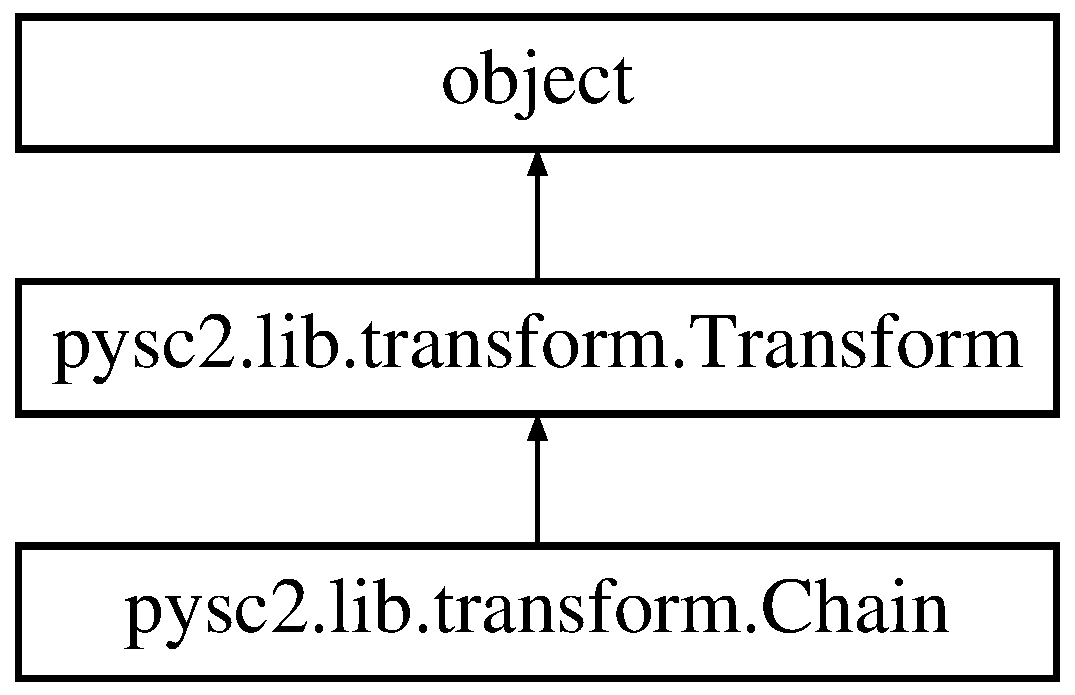
\includegraphics[height=3.000000cm]{classpysc2_1_1lib_1_1transform_1_1_chain}
\end{center}
\end{figure}
\subsection*{Public Member Functions}
\begin{DoxyCompactItemize}
\item 
def \mbox{\hyperlink{classpysc2_1_1lib_1_1transform_1_1_chain_a1d57ca10d7be4c654ce06576bbb4ad18}{\+\_\+\+\_\+init\+\_\+\+\_\+}} (self, args)
\item 
def \mbox{\hyperlink{classpysc2_1_1lib_1_1transform_1_1_chain_a25df9664f373ccc03b5b10a8f377403f}{fwd\+\_\+dist}} (self, dist)
\item 
def \mbox{\hyperlink{classpysc2_1_1lib_1_1transform_1_1_chain_a5f3eaf18a7e2894fe6cda71aa2494f90}{fwd\+\_\+pt}} (self, pt)
\item 
def \mbox{\hyperlink{classpysc2_1_1lib_1_1transform_1_1_chain_aba80172f3b617b23cf5b77157d9eec39}{back\+\_\+dist}} (self, dist)
\item 
def \mbox{\hyperlink{classpysc2_1_1lib_1_1transform_1_1_chain_a120a678dc48fe4c20793c451a6e97ee1}{back\+\_\+pt}} (self, pt)
\item 
def \mbox{\hyperlink{classpysc2_1_1lib_1_1transform_1_1_chain_ab85b58ce2f473803c1e19ff01efc2dcb}{\+\_\+\+\_\+str\+\_\+\+\_\+}} (self)
\end{DoxyCompactItemize}
\subsection*{Public Attributes}
\begin{DoxyCompactItemize}
\item 
\mbox{\hyperlink{classpysc2_1_1lib_1_1transform_1_1_chain_a445a392e9d972836f6ec6d3b43018192}{transforms}}
\end{DoxyCompactItemize}


\subsection{Detailed Description}
\begin{DoxyVerb}Chain a set of transforms: Chain(a_to_b, b_to_c) => a_to_c.\end{DoxyVerb}
 

\subsection{Constructor \& Destructor Documentation}
\mbox{\Hypertarget{classpysc2_1_1lib_1_1transform_1_1_chain_a1d57ca10d7be4c654ce06576bbb4ad18}\label{classpysc2_1_1lib_1_1transform_1_1_chain_a1d57ca10d7be4c654ce06576bbb4ad18}} 
\index{pysc2\+::lib\+::transform\+::\+Chain@{pysc2\+::lib\+::transform\+::\+Chain}!\+\_\+\+\_\+init\+\_\+\+\_\+@{\+\_\+\+\_\+init\+\_\+\+\_\+}}
\index{\+\_\+\+\_\+init\+\_\+\+\_\+@{\+\_\+\+\_\+init\+\_\+\+\_\+}!pysc2\+::lib\+::transform\+::\+Chain@{pysc2\+::lib\+::transform\+::\+Chain}}
\subsubsection{\texorpdfstring{\+\_\+\+\_\+init\+\_\+\+\_\+()}{\_\_init\_\_()}}
{\footnotesize\ttfamily def pysc2.\+lib.\+transform.\+Chain.\+\_\+\+\_\+init\+\_\+\+\_\+ (\begin{DoxyParamCaption}\item[{}]{self,  }\item[{}]{args }\end{DoxyParamCaption})}



\subsection{Member Function Documentation}
\mbox{\Hypertarget{classpysc2_1_1lib_1_1transform_1_1_chain_ab85b58ce2f473803c1e19ff01efc2dcb}\label{classpysc2_1_1lib_1_1transform_1_1_chain_ab85b58ce2f473803c1e19ff01efc2dcb}} 
\index{pysc2\+::lib\+::transform\+::\+Chain@{pysc2\+::lib\+::transform\+::\+Chain}!\+\_\+\+\_\+str\+\_\+\+\_\+@{\+\_\+\+\_\+str\+\_\+\+\_\+}}
\index{\+\_\+\+\_\+str\+\_\+\+\_\+@{\+\_\+\+\_\+str\+\_\+\+\_\+}!pysc2\+::lib\+::transform\+::\+Chain@{pysc2\+::lib\+::transform\+::\+Chain}}
\subsubsection{\texorpdfstring{\+\_\+\+\_\+str\+\_\+\+\_\+()}{\_\_str\_\_()}}
{\footnotesize\ttfamily def pysc2.\+lib.\+transform.\+Chain.\+\_\+\+\_\+str\+\_\+\+\_\+ (\begin{DoxyParamCaption}\item[{}]{self }\end{DoxyParamCaption})}

\mbox{\Hypertarget{classpysc2_1_1lib_1_1transform_1_1_chain_aba80172f3b617b23cf5b77157d9eec39}\label{classpysc2_1_1lib_1_1transform_1_1_chain_aba80172f3b617b23cf5b77157d9eec39}} 
\index{pysc2\+::lib\+::transform\+::\+Chain@{pysc2\+::lib\+::transform\+::\+Chain}!back\+\_\+dist@{back\+\_\+dist}}
\index{back\+\_\+dist@{back\+\_\+dist}!pysc2\+::lib\+::transform\+::\+Chain@{pysc2\+::lib\+::transform\+::\+Chain}}
\subsubsection{\texorpdfstring{back\+\_\+dist()}{back\_dist()}}
{\footnotesize\ttfamily def pysc2.\+lib.\+transform.\+Chain.\+back\+\_\+dist (\begin{DoxyParamCaption}\item[{}]{self,  }\item[{}]{dist }\end{DoxyParamCaption})}

\mbox{\Hypertarget{classpysc2_1_1lib_1_1transform_1_1_chain_a120a678dc48fe4c20793c451a6e97ee1}\label{classpysc2_1_1lib_1_1transform_1_1_chain_a120a678dc48fe4c20793c451a6e97ee1}} 
\index{pysc2\+::lib\+::transform\+::\+Chain@{pysc2\+::lib\+::transform\+::\+Chain}!back\+\_\+pt@{back\+\_\+pt}}
\index{back\+\_\+pt@{back\+\_\+pt}!pysc2\+::lib\+::transform\+::\+Chain@{pysc2\+::lib\+::transform\+::\+Chain}}
\subsubsection{\texorpdfstring{back\+\_\+pt()}{back\_pt()}}
{\footnotesize\ttfamily def pysc2.\+lib.\+transform.\+Chain.\+back\+\_\+pt (\begin{DoxyParamCaption}\item[{}]{self,  }\item[{}]{pt }\end{DoxyParamCaption})}

\mbox{\Hypertarget{classpysc2_1_1lib_1_1transform_1_1_chain_a25df9664f373ccc03b5b10a8f377403f}\label{classpysc2_1_1lib_1_1transform_1_1_chain_a25df9664f373ccc03b5b10a8f377403f}} 
\index{pysc2\+::lib\+::transform\+::\+Chain@{pysc2\+::lib\+::transform\+::\+Chain}!fwd\+\_\+dist@{fwd\+\_\+dist}}
\index{fwd\+\_\+dist@{fwd\+\_\+dist}!pysc2\+::lib\+::transform\+::\+Chain@{pysc2\+::lib\+::transform\+::\+Chain}}
\subsubsection{\texorpdfstring{fwd\+\_\+dist()}{fwd\_dist()}}
{\footnotesize\ttfamily def pysc2.\+lib.\+transform.\+Chain.\+fwd\+\_\+dist (\begin{DoxyParamCaption}\item[{}]{self,  }\item[{}]{dist }\end{DoxyParamCaption})}

\mbox{\Hypertarget{classpysc2_1_1lib_1_1transform_1_1_chain_a5f3eaf18a7e2894fe6cda71aa2494f90}\label{classpysc2_1_1lib_1_1transform_1_1_chain_a5f3eaf18a7e2894fe6cda71aa2494f90}} 
\index{pysc2\+::lib\+::transform\+::\+Chain@{pysc2\+::lib\+::transform\+::\+Chain}!fwd\+\_\+pt@{fwd\+\_\+pt}}
\index{fwd\+\_\+pt@{fwd\+\_\+pt}!pysc2\+::lib\+::transform\+::\+Chain@{pysc2\+::lib\+::transform\+::\+Chain}}
\subsubsection{\texorpdfstring{fwd\+\_\+pt()}{fwd\_pt()}}
{\footnotesize\ttfamily def pysc2.\+lib.\+transform.\+Chain.\+fwd\+\_\+pt (\begin{DoxyParamCaption}\item[{}]{self,  }\item[{}]{pt }\end{DoxyParamCaption})}



\subsection{Member Data Documentation}
\mbox{\Hypertarget{classpysc2_1_1lib_1_1transform_1_1_chain_a445a392e9d972836f6ec6d3b43018192}\label{classpysc2_1_1lib_1_1transform_1_1_chain_a445a392e9d972836f6ec6d3b43018192}} 
\index{pysc2\+::lib\+::transform\+::\+Chain@{pysc2\+::lib\+::transform\+::\+Chain}!transforms@{transforms}}
\index{transforms@{transforms}!pysc2\+::lib\+::transform\+::\+Chain@{pysc2\+::lib\+::transform\+::\+Chain}}
\subsubsection{\texorpdfstring{transforms}{transforms}}
{\footnotesize\ttfamily pysc2.\+lib.\+transform.\+Chain.\+transforms}



The documentation for this class was generated from the following file\+:\begin{DoxyCompactItemize}
\item 
lib/\mbox{\hyperlink{transform_8py}{transform.\+py}}\end{DoxyCompactItemize}

\hypertarget{classpysc2_1_1agents_1_1scripted__agent_1_1_collect_mineral_shards}{}\section{pysc2.\+agents.\+scripted\+\_\+agent.\+Collect\+Mineral\+Shards Class Reference}
\label{classpysc2_1_1agents_1_1scripted__agent_1_1_collect_mineral_shards}\index{pysc2.\+agents.\+scripted\+\_\+agent.\+Collect\+Mineral\+Shards@{pysc2.\+agents.\+scripted\+\_\+agent.\+Collect\+Mineral\+Shards}}
Inheritance diagram for pysc2.\+agents.\+scripted\+\_\+agent.\+Collect\+Mineral\+Shards\+:\begin{figure}[H]
\begin{center}
\leavevmode
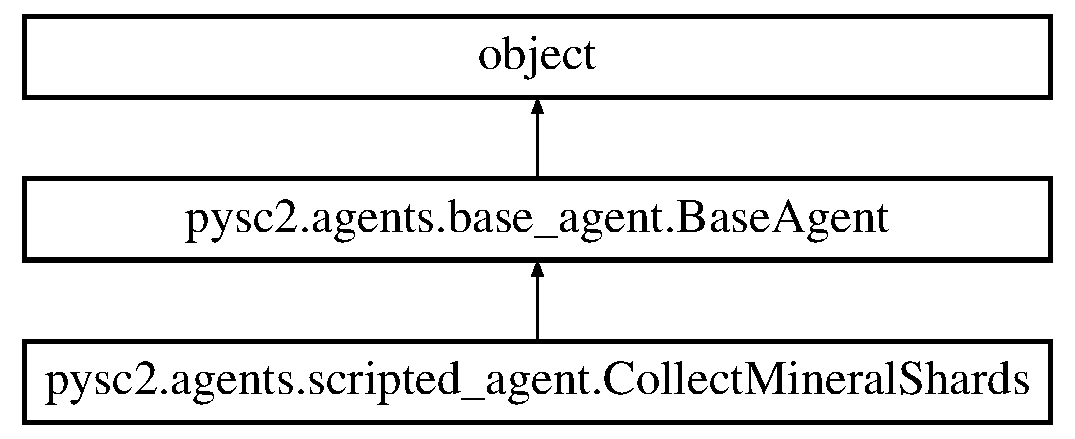
\includegraphics[height=3.000000cm]{classpysc2_1_1agents_1_1scripted__agent_1_1_collect_mineral_shards}
\end{center}
\end{figure}
\subsection*{Public Member Functions}
\begin{DoxyCompactItemize}
\item 
def \mbox{\hyperlink{classpysc2_1_1agents_1_1scripted__agent_1_1_collect_mineral_shards_a74fd157c889f76bb587eb46c3ff83f7e}{step}} (self, obs)
\end{DoxyCompactItemize}
\subsection*{Additional Inherited Members}


\subsection{Detailed Description}
\begin{DoxyVerb}An agent specifically for solving the CollectMineralShards map.\end{DoxyVerb}
 

\subsection{Member Function Documentation}
\mbox{\Hypertarget{classpysc2_1_1agents_1_1scripted__agent_1_1_collect_mineral_shards_a74fd157c889f76bb587eb46c3ff83f7e}\label{classpysc2_1_1agents_1_1scripted__agent_1_1_collect_mineral_shards_a74fd157c889f76bb587eb46c3ff83f7e}} 
\index{pysc2\+::agents\+::scripted\+\_\+agent\+::\+Collect\+Mineral\+Shards@{pysc2\+::agents\+::scripted\+\_\+agent\+::\+Collect\+Mineral\+Shards}!step@{step}}
\index{step@{step}!pysc2\+::agents\+::scripted\+\_\+agent\+::\+Collect\+Mineral\+Shards@{pysc2\+::agents\+::scripted\+\_\+agent\+::\+Collect\+Mineral\+Shards}}
\subsubsection{\texorpdfstring{step()}{step()}}
{\footnotesize\ttfamily def pysc2.\+agents.\+scripted\+\_\+agent.\+Collect\+Mineral\+Shards.\+step (\begin{DoxyParamCaption}\item[{}]{self,  }\item[{}]{obs }\end{DoxyParamCaption})}



The documentation for this class was generated from the following file\+:\begin{DoxyCompactItemize}
\item 
agents/\mbox{\hyperlink{scripted__agent_8py}{scripted\+\_\+agent.\+py}}\end{DoxyCompactItemize}

\hypertarget{classpysc2_1_1agents_1_1scripted__agent_1_1_collect_mineral_shards_feature_units}{}\section{pysc2.\+agents.\+scripted\+\_\+agent.\+Collect\+Mineral\+Shards\+Feature\+Units Class Reference}
\label{classpysc2_1_1agents_1_1scripted__agent_1_1_collect_mineral_shards_feature_units}\index{pysc2.\+agents.\+scripted\+\_\+agent.\+Collect\+Mineral\+Shards\+Feature\+Units@{pysc2.\+agents.\+scripted\+\_\+agent.\+Collect\+Mineral\+Shards\+Feature\+Units}}
Inheritance diagram for pysc2.\+agents.\+scripted\+\_\+agent.\+Collect\+Mineral\+Shards\+Feature\+Units\+:\begin{figure}[H]
\begin{center}
\leavevmode
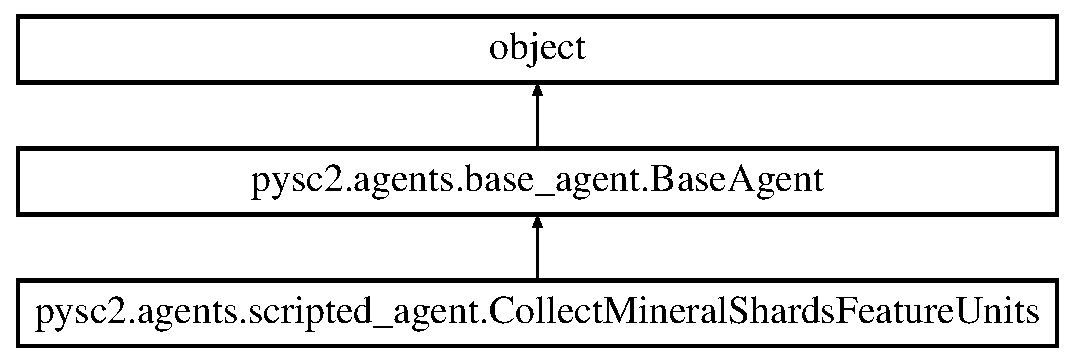
\includegraphics[height=3.000000cm]{classpysc2_1_1agents_1_1scripted__agent_1_1_collect_mineral_shards_feature_units}
\end{center}
\end{figure}
\subsection*{Public Member Functions}
\begin{DoxyCompactItemize}
\item 
def \mbox{\hyperlink{classpysc2_1_1agents_1_1scripted__agent_1_1_collect_mineral_shards_feature_units_a6f486dbd7973e7d925e70e72ffe44aff}{setup}} (self, \mbox{\hyperlink{classpysc2_1_1agents_1_1base__agent_1_1_base_agent_ad6cefb81724b9d234887cea543c4f06e}{obs\+\_\+spec}}, \mbox{\hyperlink{classpysc2_1_1agents_1_1base__agent_1_1_base_agent_a550b216b98ae40b2da1b2fd9015d3019}{action\+\_\+spec}})
\item 
def \mbox{\hyperlink{classpysc2_1_1agents_1_1scripted__agent_1_1_collect_mineral_shards_feature_units_a46a2b6dc43b5fd8e535505d25a29ea1d}{reset}} (self)
\item 
def \mbox{\hyperlink{classpysc2_1_1agents_1_1scripted__agent_1_1_collect_mineral_shards_feature_units_ac09e7d23c9cc9ad8b7a26c42561bd4b0}{step}} (self, obs)
\end{DoxyCompactItemize}
\subsection*{Additional Inherited Members}


\subsection{Detailed Description}
\begin{DoxyVerb}An agent for solving the CollectMineralShards map with feature units.

Controls the two marines independently:
- select marine
- move to nearest mineral shard that wasn't the previous target
- swap marine and repeat
\end{DoxyVerb}
 

\subsection{Member Function Documentation}
\mbox{\Hypertarget{classpysc2_1_1agents_1_1scripted__agent_1_1_collect_mineral_shards_feature_units_a46a2b6dc43b5fd8e535505d25a29ea1d}\label{classpysc2_1_1agents_1_1scripted__agent_1_1_collect_mineral_shards_feature_units_a46a2b6dc43b5fd8e535505d25a29ea1d}} 
\index{pysc2\+::agents\+::scripted\+\_\+agent\+::\+Collect\+Mineral\+Shards\+Feature\+Units@{pysc2\+::agents\+::scripted\+\_\+agent\+::\+Collect\+Mineral\+Shards\+Feature\+Units}!reset@{reset}}
\index{reset@{reset}!pysc2\+::agents\+::scripted\+\_\+agent\+::\+Collect\+Mineral\+Shards\+Feature\+Units@{pysc2\+::agents\+::scripted\+\_\+agent\+::\+Collect\+Mineral\+Shards\+Feature\+Units}}
\subsubsection{\texorpdfstring{reset()}{reset()}}
{\footnotesize\ttfamily def pysc2.\+agents.\+scripted\+\_\+agent.\+Collect\+Mineral\+Shards\+Feature\+Units.\+reset (\begin{DoxyParamCaption}\item[{}]{self }\end{DoxyParamCaption})}

\mbox{\Hypertarget{classpysc2_1_1agents_1_1scripted__agent_1_1_collect_mineral_shards_feature_units_a6f486dbd7973e7d925e70e72ffe44aff}\label{classpysc2_1_1agents_1_1scripted__agent_1_1_collect_mineral_shards_feature_units_a6f486dbd7973e7d925e70e72ffe44aff}} 
\index{pysc2\+::agents\+::scripted\+\_\+agent\+::\+Collect\+Mineral\+Shards\+Feature\+Units@{pysc2\+::agents\+::scripted\+\_\+agent\+::\+Collect\+Mineral\+Shards\+Feature\+Units}!setup@{setup}}
\index{setup@{setup}!pysc2\+::agents\+::scripted\+\_\+agent\+::\+Collect\+Mineral\+Shards\+Feature\+Units@{pysc2\+::agents\+::scripted\+\_\+agent\+::\+Collect\+Mineral\+Shards\+Feature\+Units}}
\subsubsection{\texorpdfstring{setup()}{setup()}}
{\footnotesize\ttfamily def pysc2.\+agents.\+scripted\+\_\+agent.\+Collect\+Mineral\+Shards\+Feature\+Units.\+setup (\begin{DoxyParamCaption}\item[{}]{self,  }\item[{}]{obs\+\_\+spec,  }\item[{}]{action\+\_\+spec }\end{DoxyParamCaption})}

\mbox{\Hypertarget{classpysc2_1_1agents_1_1scripted__agent_1_1_collect_mineral_shards_feature_units_ac09e7d23c9cc9ad8b7a26c42561bd4b0}\label{classpysc2_1_1agents_1_1scripted__agent_1_1_collect_mineral_shards_feature_units_ac09e7d23c9cc9ad8b7a26c42561bd4b0}} 
\index{pysc2\+::agents\+::scripted\+\_\+agent\+::\+Collect\+Mineral\+Shards\+Feature\+Units@{pysc2\+::agents\+::scripted\+\_\+agent\+::\+Collect\+Mineral\+Shards\+Feature\+Units}!step@{step}}
\index{step@{step}!pysc2\+::agents\+::scripted\+\_\+agent\+::\+Collect\+Mineral\+Shards\+Feature\+Units@{pysc2\+::agents\+::scripted\+\_\+agent\+::\+Collect\+Mineral\+Shards\+Feature\+Units}}
\subsubsection{\texorpdfstring{step()}{step()}}
{\footnotesize\ttfamily def pysc2.\+agents.\+scripted\+\_\+agent.\+Collect\+Mineral\+Shards\+Feature\+Units.\+step (\begin{DoxyParamCaption}\item[{}]{self,  }\item[{}]{obs }\end{DoxyParamCaption})}



The documentation for this class was generated from the following file\+:\begin{DoxyCompactItemize}
\item 
agents/\mbox{\hyperlink{scripted__agent_8py}{scripted\+\_\+agent.\+py}}\end{DoxyCompactItemize}

\hypertarget{classpysc2_1_1lib_1_1colors_1_1_color}{}\section{pysc2.\+lib.\+colors.\+Color Class Reference}
\label{classpysc2_1_1lib_1_1colors_1_1_color}\index{pysc2.\+lib.\+colors.\+Color@{pysc2.\+lib.\+colors.\+Color}}
Inheritance diagram for pysc2.\+lib.\+colors.\+Color\+:\begin{figure}[H]
\begin{center}
\leavevmode
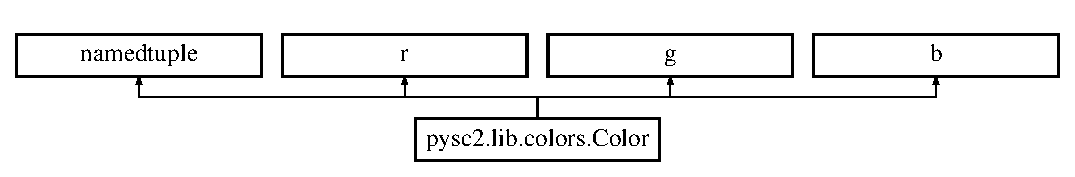
\includegraphics[height=1.931034cm]{classpysc2_1_1lib_1_1colors_1_1_color}
\end{center}
\end{figure}
\subsection*{Public Member Functions}
\begin{DoxyCompactItemize}
\item 
def \mbox{\hyperlink{classpysc2_1_1lib_1_1colors_1_1_color_a4f85933c31b5eee882ee02bc276c2910}{set}} (self, r=None, g=None, b=None)
\item 
def \mbox{\hyperlink{classpysc2_1_1lib_1_1colors_1_1_color_a38a169169ccba8887056f2411b48919a}{round}} (self)
\item 
def \mbox{\hyperlink{classpysc2_1_1lib_1_1colors_1_1_color_a1d574e03aa1e9eaedbd7693efcd96c49}{floor}} (self)
\item 
def \mbox{\hyperlink{classpysc2_1_1lib_1_1colors_1_1_color_aa0516d088a354d745b86a855c972d8ba}{ceil}} (self)
\item 
def \mbox{\hyperlink{classpysc2_1_1lib_1_1colors_1_1_color_ad3c3b8cc2e506b1d2aaedc50aae52016}{\+\_\+\+\_\+str\+\_\+\+\_\+}} (self)
\item 
def \mbox{\hyperlink{classpysc2_1_1lib_1_1colors_1_1_color_af1b1d0a84bcc91484781007d63e6113b}{\+\_\+\+\_\+add\+\_\+\+\_\+}} (self, o)
\item 
def \mbox{\hyperlink{classpysc2_1_1lib_1_1colors_1_1_color_af38ed2fff40bacddd1dd02d9676f7486}{\+\_\+\+\_\+sub\+\_\+\+\_\+}} (self, o)
\item 
def \mbox{\hyperlink{classpysc2_1_1lib_1_1colors_1_1_color_a4cc27cb2b3f1f2be14e671f0def6c9da}{\+\_\+\+\_\+mul\+\_\+\+\_\+}} (self, val)
\item 
def \mbox{\hyperlink{classpysc2_1_1lib_1_1colors_1_1_color_a232910e9fbb61b4ed2a71c70223be937}{\+\_\+\+\_\+truediv\+\_\+\+\_\+}} (self, val)
\item 
def \mbox{\hyperlink{classpysc2_1_1lib_1_1colors_1_1_color_a1b8de342848c1a509ea27131ce6aedc3}{\+\_\+\+\_\+floordiv\+\_\+\+\_\+}} (self, val)
\end{DoxyCompactItemize}


\subsection{Detailed Description}
\begin{DoxyVerb}A basic Color class.\end{DoxyVerb}
 

\subsection{Member Function Documentation}
\mbox{\Hypertarget{classpysc2_1_1lib_1_1colors_1_1_color_af1b1d0a84bcc91484781007d63e6113b}\label{classpysc2_1_1lib_1_1colors_1_1_color_af1b1d0a84bcc91484781007d63e6113b}} 
\index{pysc2\+::lib\+::colors\+::\+Color@{pysc2\+::lib\+::colors\+::\+Color}!\+\_\+\+\_\+add\+\_\+\+\_\+@{\+\_\+\+\_\+add\+\_\+\+\_\+}}
\index{\+\_\+\+\_\+add\+\_\+\+\_\+@{\+\_\+\+\_\+add\+\_\+\+\_\+}!pysc2\+::lib\+::colors\+::\+Color@{pysc2\+::lib\+::colors\+::\+Color}}
\subsubsection{\texorpdfstring{\+\_\+\+\_\+add\+\_\+\+\_\+()}{\_\_add\_\_()}}
{\footnotesize\ttfamily def pysc2.\+lib.\+colors.\+Color.\+\_\+\+\_\+add\+\_\+\+\_\+ (\begin{DoxyParamCaption}\item[{}]{self,  }\item[{}]{o }\end{DoxyParamCaption})}

\mbox{\Hypertarget{classpysc2_1_1lib_1_1colors_1_1_color_a1b8de342848c1a509ea27131ce6aedc3}\label{classpysc2_1_1lib_1_1colors_1_1_color_a1b8de342848c1a509ea27131ce6aedc3}} 
\index{pysc2\+::lib\+::colors\+::\+Color@{pysc2\+::lib\+::colors\+::\+Color}!\+\_\+\+\_\+floordiv\+\_\+\+\_\+@{\+\_\+\+\_\+floordiv\+\_\+\+\_\+}}
\index{\+\_\+\+\_\+floordiv\+\_\+\+\_\+@{\+\_\+\+\_\+floordiv\+\_\+\+\_\+}!pysc2\+::lib\+::colors\+::\+Color@{pysc2\+::lib\+::colors\+::\+Color}}
\subsubsection{\texorpdfstring{\+\_\+\+\_\+floordiv\+\_\+\+\_\+()}{\_\_floordiv\_\_()}}
{\footnotesize\ttfamily def pysc2.\+lib.\+colors.\+Color.\+\_\+\+\_\+floordiv\+\_\+\+\_\+ (\begin{DoxyParamCaption}\item[{}]{self,  }\item[{}]{val }\end{DoxyParamCaption})}

\mbox{\Hypertarget{classpysc2_1_1lib_1_1colors_1_1_color_a4cc27cb2b3f1f2be14e671f0def6c9da}\label{classpysc2_1_1lib_1_1colors_1_1_color_a4cc27cb2b3f1f2be14e671f0def6c9da}} 
\index{pysc2\+::lib\+::colors\+::\+Color@{pysc2\+::lib\+::colors\+::\+Color}!\+\_\+\+\_\+mul\+\_\+\+\_\+@{\+\_\+\+\_\+mul\+\_\+\+\_\+}}
\index{\+\_\+\+\_\+mul\+\_\+\+\_\+@{\+\_\+\+\_\+mul\+\_\+\+\_\+}!pysc2\+::lib\+::colors\+::\+Color@{pysc2\+::lib\+::colors\+::\+Color}}
\subsubsection{\texorpdfstring{\+\_\+\+\_\+mul\+\_\+\+\_\+()}{\_\_mul\_\_()}}
{\footnotesize\ttfamily def pysc2.\+lib.\+colors.\+Color.\+\_\+\+\_\+mul\+\_\+\+\_\+ (\begin{DoxyParamCaption}\item[{}]{self,  }\item[{}]{val }\end{DoxyParamCaption})}

\mbox{\Hypertarget{classpysc2_1_1lib_1_1colors_1_1_color_ad3c3b8cc2e506b1d2aaedc50aae52016}\label{classpysc2_1_1lib_1_1colors_1_1_color_ad3c3b8cc2e506b1d2aaedc50aae52016}} 
\index{pysc2\+::lib\+::colors\+::\+Color@{pysc2\+::lib\+::colors\+::\+Color}!\+\_\+\+\_\+str\+\_\+\+\_\+@{\+\_\+\+\_\+str\+\_\+\+\_\+}}
\index{\+\_\+\+\_\+str\+\_\+\+\_\+@{\+\_\+\+\_\+str\+\_\+\+\_\+}!pysc2\+::lib\+::colors\+::\+Color@{pysc2\+::lib\+::colors\+::\+Color}}
\subsubsection{\texorpdfstring{\+\_\+\+\_\+str\+\_\+\+\_\+()}{\_\_str\_\_()}}
{\footnotesize\ttfamily def pysc2.\+lib.\+colors.\+Color.\+\_\+\+\_\+str\+\_\+\+\_\+ (\begin{DoxyParamCaption}\item[{}]{self }\end{DoxyParamCaption})}

\mbox{\Hypertarget{classpysc2_1_1lib_1_1colors_1_1_color_af38ed2fff40bacddd1dd02d9676f7486}\label{classpysc2_1_1lib_1_1colors_1_1_color_af38ed2fff40bacddd1dd02d9676f7486}} 
\index{pysc2\+::lib\+::colors\+::\+Color@{pysc2\+::lib\+::colors\+::\+Color}!\+\_\+\+\_\+sub\+\_\+\+\_\+@{\+\_\+\+\_\+sub\+\_\+\+\_\+}}
\index{\+\_\+\+\_\+sub\+\_\+\+\_\+@{\+\_\+\+\_\+sub\+\_\+\+\_\+}!pysc2\+::lib\+::colors\+::\+Color@{pysc2\+::lib\+::colors\+::\+Color}}
\subsubsection{\texorpdfstring{\+\_\+\+\_\+sub\+\_\+\+\_\+()}{\_\_sub\_\_()}}
{\footnotesize\ttfamily def pysc2.\+lib.\+colors.\+Color.\+\_\+\+\_\+sub\+\_\+\+\_\+ (\begin{DoxyParamCaption}\item[{}]{self,  }\item[{}]{o }\end{DoxyParamCaption})}

\mbox{\Hypertarget{classpysc2_1_1lib_1_1colors_1_1_color_a232910e9fbb61b4ed2a71c70223be937}\label{classpysc2_1_1lib_1_1colors_1_1_color_a232910e9fbb61b4ed2a71c70223be937}} 
\index{pysc2\+::lib\+::colors\+::\+Color@{pysc2\+::lib\+::colors\+::\+Color}!\+\_\+\+\_\+truediv\+\_\+\+\_\+@{\+\_\+\+\_\+truediv\+\_\+\+\_\+}}
\index{\+\_\+\+\_\+truediv\+\_\+\+\_\+@{\+\_\+\+\_\+truediv\+\_\+\+\_\+}!pysc2\+::lib\+::colors\+::\+Color@{pysc2\+::lib\+::colors\+::\+Color}}
\subsubsection{\texorpdfstring{\+\_\+\+\_\+truediv\+\_\+\+\_\+()}{\_\_truediv\_\_()}}
{\footnotesize\ttfamily def pysc2.\+lib.\+colors.\+Color.\+\_\+\+\_\+truediv\+\_\+\+\_\+ (\begin{DoxyParamCaption}\item[{}]{self,  }\item[{}]{val }\end{DoxyParamCaption})}

\mbox{\Hypertarget{classpysc2_1_1lib_1_1colors_1_1_color_aa0516d088a354d745b86a855c972d8ba}\label{classpysc2_1_1lib_1_1colors_1_1_color_aa0516d088a354d745b86a855c972d8ba}} 
\index{pysc2\+::lib\+::colors\+::\+Color@{pysc2\+::lib\+::colors\+::\+Color}!ceil@{ceil}}
\index{ceil@{ceil}!pysc2\+::lib\+::colors\+::\+Color@{pysc2\+::lib\+::colors\+::\+Color}}
\subsubsection{\texorpdfstring{ceil()}{ceil()}}
{\footnotesize\ttfamily def pysc2.\+lib.\+colors.\+Color.\+ceil (\begin{DoxyParamCaption}\item[{}]{self }\end{DoxyParamCaption})}

\mbox{\Hypertarget{classpysc2_1_1lib_1_1colors_1_1_color_a1d574e03aa1e9eaedbd7693efcd96c49}\label{classpysc2_1_1lib_1_1colors_1_1_color_a1d574e03aa1e9eaedbd7693efcd96c49}} 
\index{pysc2\+::lib\+::colors\+::\+Color@{pysc2\+::lib\+::colors\+::\+Color}!floor@{floor}}
\index{floor@{floor}!pysc2\+::lib\+::colors\+::\+Color@{pysc2\+::lib\+::colors\+::\+Color}}
\subsubsection{\texorpdfstring{floor()}{floor()}}
{\footnotesize\ttfamily def pysc2.\+lib.\+colors.\+Color.\+floor (\begin{DoxyParamCaption}\item[{}]{self }\end{DoxyParamCaption})}

\mbox{\Hypertarget{classpysc2_1_1lib_1_1colors_1_1_color_a38a169169ccba8887056f2411b48919a}\label{classpysc2_1_1lib_1_1colors_1_1_color_a38a169169ccba8887056f2411b48919a}} 
\index{pysc2\+::lib\+::colors\+::\+Color@{pysc2\+::lib\+::colors\+::\+Color}!round@{round}}
\index{round@{round}!pysc2\+::lib\+::colors\+::\+Color@{pysc2\+::lib\+::colors\+::\+Color}}
\subsubsection{\texorpdfstring{round()}{round()}}
{\footnotesize\ttfamily def pysc2.\+lib.\+colors.\+Color.\+round (\begin{DoxyParamCaption}\item[{}]{self }\end{DoxyParamCaption})}

\mbox{\Hypertarget{classpysc2_1_1lib_1_1colors_1_1_color_a4f85933c31b5eee882ee02bc276c2910}\label{classpysc2_1_1lib_1_1colors_1_1_color_a4f85933c31b5eee882ee02bc276c2910}} 
\index{pysc2\+::lib\+::colors\+::\+Color@{pysc2\+::lib\+::colors\+::\+Color}!set@{set}}
\index{set@{set}!pysc2\+::lib\+::colors\+::\+Color@{pysc2\+::lib\+::colors\+::\+Color}}
\subsubsection{\texorpdfstring{set()}{set()}}
{\footnotesize\ttfamily def pysc2.\+lib.\+colors.\+Color.\+set (\begin{DoxyParamCaption}\item[{}]{self,  }\item[{}]{r = {\ttfamily None},  }\item[{}]{g = {\ttfamily None},  }\item[{}]{b = {\ttfamily None} }\end{DoxyParamCaption})}



The documentation for this class was generated from the following file\+:\begin{DoxyCompactItemize}
\item 
lib/\mbox{\hyperlink{colors_8py}{colors.\+py}}\end{DoxyCompactItemize}

\hypertarget{classpysc2_1_1tests_1_1replay__obs__test_1_1_config}{}\section{pysc2.\+tests.\+replay\+\_\+obs\+\_\+test.\+Config Class Reference}
\label{classpysc2_1_1tests_1_1replay__obs__test_1_1_config}\index{pysc2.\+tests.\+replay\+\_\+obs\+\_\+test.\+Config@{pysc2.\+tests.\+replay\+\_\+obs\+\_\+test.\+Config}}
Inheritance diagram for pysc2.\+tests.\+replay\+\_\+obs\+\_\+test.\+Config\+:\begin{figure}[H]
\begin{center}
\leavevmode
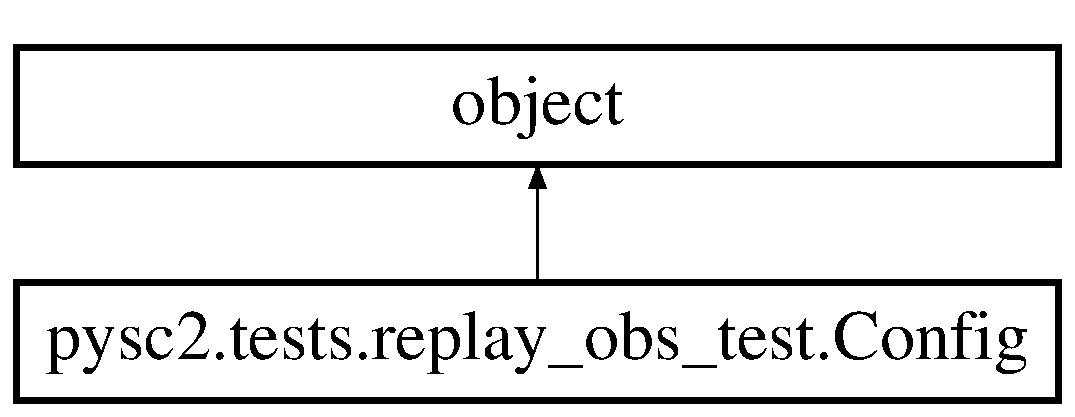
\includegraphics[height=2.000000cm]{classpysc2_1_1tests_1_1replay__obs__test_1_1_config}
\end{center}
\end{figure}
\subsection*{Public Member Functions}
\begin{DoxyCompactItemize}
\item 
def \mbox{\hyperlink{classpysc2_1_1tests_1_1replay__obs__test_1_1_config_a93f88965c69c40958a8953bb0d1ff86f}{\+\_\+\+\_\+init\+\_\+\+\_\+}} (self)
\end{DoxyCompactItemize}
\subsection*{Public Attributes}
\begin{DoxyCompactItemize}
\item 
\mbox{\hyperlink{classpysc2_1_1tests_1_1replay__obs__test_1_1_config_a718f77f4c6ea365e1bca95a4223ce0bf}{map\+\_\+name}}
\item 
\mbox{\hyperlink{classpysc2_1_1tests_1_1replay__obs__test_1_1_config_a651e8aa31086c011dd0a7330346affe1}{camera\+\_\+width}}
\item 
\mbox{\hyperlink{classpysc2_1_1tests_1_1replay__obs__test_1_1_config_aaf049ddbfd4a171cf08ef217a981451a}{random\+\_\+seed}}
\item 
\mbox{\hyperlink{classpysc2_1_1tests_1_1replay__obs__test_1_1_config_ab14251df14bce385ecb13b6676e3fa1e}{interface}}
\item 
\mbox{\hyperlink{classpysc2_1_1tests_1_1replay__obs__test_1_1_config_a688afdf1bec9d559e11298cb1a16a6d4}{actions}}
\item 
\mbox{\hyperlink{classpysc2_1_1tests_1_1replay__obs__test_1_1_config_a138bf9778d63f8e2211c21f93b968229}{num\+\_\+observations}}
\item 
\mbox{\hyperlink{classpysc2_1_1tests_1_1replay__obs__test_1_1_config_ad37c2e73d565130c37c8a0e2e065029b}{player\+\_\+id}}
\end{DoxyCompactItemize}


\subsection{Detailed Description}
\begin{DoxyVerb}Holds the configuration options.\end{DoxyVerb}
 

\subsection{Constructor \& Destructor Documentation}
\mbox{\Hypertarget{classpysc2_1_1tests_1_1replay__obs__test_1_1_config_a93f88965c69c40958a8953bb0d1ff86f}\label{classpysc2_1_1tests_1_1replay__obs__test_1_1_config_a93f88965c69c40958a8953bb0d1ff86f}} 
\index{pysc2\+::tests\+::replay\+\_\+obs\+\_\+test\+::\+Config@{pysc2\+::tests\+::replay\+\_\+obs\+\_\+test\+::\+Config}!\+\_\+\+\_\+init\+\_\+\+\_\+@{\+\_\+\+\_\+init\+\_\+\+\_\+}}
\index{\+\_\+\+\_\+init\+\_\+\+\_\+@{\+\_\+\+\_\+init\+\_\+\+\_\+}!pysc2\+::tests\+::replay\+\_\+obs\+\_\+test\+::\+Config@{pysc2\+::tests\+::replay\+\_\+obs\+\_\+test\+::\+Config}}
\subsubsection{\texorpdfstring{\+\_\+\+\_\+init\+\_\+\+\_\+()}{\_\_init\_\_()}}
{\footnotesize\ttfamily def pysc2.\+tests.\+replay\+\_\+obs\+\_\+test.\+Config.\+\_\+\+\_\+init\+\_\+\+\_\+ (\begin{DoxyParamCaption}\item[{}]{self }\end{DoxyParamCaption})}



\subsection{Member Data Documentation}
\mbox{\Hypertarget{classpysc2_1_1tests_1_1replay__obs__test_1_1_config_a688afdf1bec9d559e11298cb1a16a6d4}\label{classpysc2_1_1tests_1_1replay__obs__test_1_1_config_a688afdf1bec9d559e11298cb1a16a6d4}} 
\index{pysc2\+::tests\+::replay\+\_\+obs\+\_\+test\+::\+Config@{pysc2\+::tests\+::replay\+\_\+obs\+\_\+test\+::\+Config}!actions@{actions}}
\index{actions@{actions}!pysc2\+::tests\+::replay\+\_\+obs\+\_\+test\+::\+Config@{pysc2\+::tests\+::replay\+\_\+obs\+\_\+test\+::\+Config}}
\subsubsection{\texorpdfstring{actions}{actions}}
{\footnotesize\ttfamily pysc2.\+tests.\+replay\+\_\+obs\+\_\+test.\+Config.\+actions}

\mbox{\Hypertarget{classpysc2_1_1tests_1_1replay__obs__test_1_1_config_a651e8aa31086c011dd0a7330346affe1}\label{classpysc2_1_1tests_1_1replay__obs__test_1_1_config_a651e8aa31086c011dd0a7330346affe1}} 
\index{pysc2\+::tests\+::replay\+\_\+obs\+\_\+test\+::\+Config@{pysc2\+::tests\+::replay\+\_\+obs\+\_\+test\+::\+Config}!camera\+\_\+width@{camera\+\_\+width}}
\index{camera\+\_\+width@{camera\+\_\+width}!pysc2\+::tests\+::replay\+\_\+obs\+\_\+test\+::\+Config@{pysc2\+::tests\+::replay\+\_\+obs\+\_\+test\+::\+Config}}
\subsubsection{\texorpdfstring{camera\+\_\+width}{camera\_width}}
{\footnotesize\ttfamily pysc2.\+tests.\+replay\+\_\+obs\+\_\+test.\+Config.\+camera\+\_\+width}

\mbox{\Hypertarget{classpysc2_1_1tests_1_1replay__obs__test_1_1_config_ab14251df14bce385ecb13b6676e3fa1e}\label{classpysc2_1_1tests_1_1replay__obs__test_1_1_config_ab14251df14bce385ecb13b6676e3fa1e}} 
\index{pysc2\+::tests\+::replay\+\_\+obs\+\_\+test\+::\+Config@{pysc2\+::tests\+::replay\+\_\+obs\+\_\+test\+::\+Config}!interface@{interface}}
\index{interface@{interface}!pysc2\+::tests\+::replay\+\_\+obs\+\_\+test\+::\+Config@{pysc2\+::tests\+::replay\+\_\+obs\+\_\+test\+::\+Config}}
\subsubsection{\texorpdfstring{interface}{interface}}
{\footnotesize\ttfamily pysc2.\+tests.\+replay\+\_\+obs\+\_\+test.\+Config.\+interface}

\mbox{\Hypertarget{classpysc2_1_1tests_1_1replay__obs__test_1_1_config_a718f77f4c6ea365e1bca95a4223ce0bf}\label{classpysc2_1_1tests_1_1replay__obs__test_1_1_config_a718f77f4c6ea365e1bca95a4223ce0bf}} 
\index{pysc2\+::tests\+::replay\+\_\+obs\+\_\+test\+::\+Config@{pysc2\+::tests\+::replay\+\_\+obs\+\_\+test\+::\+Config}!map\+\_\+name@{map\+\_\+name}}
\index{map\+\_\+name@{map\+\_\+name}!pysc2\+::tests\+::replay\+\_\+obs\+\_\+test\+::\+Config@{pysc2\+::tests\+::replay\+\_\+obs\+\_\+test\+::\+Config}}
\subsubsection{\texorpdfstring{map\+\_\+name}{map\_name}}
{\footnotesize\ttfamily pysc2.\+tests.\+replay\+\_\+obs\+\_\+test.\+Config.\+map\+\_\+name}

\mbox{\Hypertarget{classpysc2_1_1tests_1_1replay__obs__test_1_1_config_a138bf9778d63f8e2211c21f93b968229}\label{classpysc2_1_1tests_1_1replay__obs__test_1_1_config_a138bf9778d63f8e2211c21f93b968229}} 
\index{pysc2\+::tests\+::replay\+\_\+obs\+\_\+test\+::\+Config@{pysc2\+::tests\+::replay\+\_\+obs\+\_\+test\+::\+Config}!num\+\_\+observations@{num\+\_\+observations}}
\index{num\+\_\+observations@{num\+\_\+observations}!pysc2\+::tests\+::replay\+\_\+obs\+\_\+test\+::\+Config@{pysc2\+::tests\+::replay\+\_\+obs\+\_\+test\+::\+Config}}
\subsubsection{\texorpdfstring{num\+\_\+observations}{num\_observations}}
{\footnotesize\ttfamily pysc2.\+tests.\+replay\+\_\+obs\+\_\+test.\+Config.\+num\+\_\+observations}

\mbox{\Hypertarget{classpysc2_1_1tests_1_1replay__obs__test_1_1_config_ad37c2e73d565130c37c8a0e2e065029b}\label{classpysc2_1_1tests_1_1replay__obs__test_1_1_config_ad37c2e73d565130c37c8a0e2e065029b}} 
\index{pysc2\+::tests\+::replay\+\_\+obs\+\_\+test\+::\+Config@{pysc2\+::tests\+::replay\+\_\+obs\+\_\+test\+::\+Config}!player\+\_\+id@{player\+\_\+id}}
\index{player\+\_\+id@{player\+\_\+id}!pysc2\+::tests\+::replay\+\_\+obs\+\_\+test\+::\+Config@{pysc2\+::tests\+::replay\+\_\+obs\+\_\+test\+::\+Config}}
\subsubsection{\texorpdfstring{player\+\_\+id}{player\_id}}
{\footnotesize\ttfamily pysc2.\+tests.\+replay\+\_\+obs\+\_\+test.\+Config.\+player\+\_\+id}

\mbox{\Hypertarget{classpysc2_1_1tests_1_1replay__obs__test_1_1_config_aaf049ddbfd4a171cf08ef217a981451a}\label{classpysc2_1_1tests_1_1replay__obs__test_1_1_config_aaf049ddbfd4a171cf08ef217a981451a}} 
\index{pysc2\+::tests\+::replay\+\_\+obs\+\_\+test\+::\+Config@{pysc2\+::tests\+::replay\+\_\+obs\+\_\+test\+::\+Config}!random\+\_\+seed@{random\+\_\+seed}}
\index{random\+\_\+seed@{random\+\_\+seed}!pysc2\+::tests\+::replay\+\_\+obs\+\_\+test\+::\+Config@{pysc2\+::tests\+::replay\+\_\+obs\+\_\+test\+::\+Config}}
\subsubsection{\texorpdfstring{random\+\_\+seed}{random\_seed}}
{\footnotesize\ttfamily pysc2.\+tests.\+replay\+\_\+obs\+\_\+test.\+Config.\+random\+\_\+seed}



The documentation for this class was generated from the following file\+:\begin{DoxyCompactItemize}
\item 
tests/\mbox{\hyperlink{replay__obs__test_8py}{replay\+\_\+obs\+\_\+test.\+py}}\end{DoxyCompactItemize}

\hypertarget{classpysc2_1_1lib_1_1remote__controller_1_1_connect_error}{}\section{pysc2.\+lib.\+remote\+\_\+controller.\+Connect\+Error Class Reference}
\label{classpysc2_1_1lib_1_1remote__controller_1_1_connect_error}\index{pysc2.\+lib.\+remote\+\_\+controller.\+Connect\+Error@{pysc2.\+lib.\+remote\+\_\+controller.\+Connect\+Error}}
Inheritance diagram for pysc2.\+lib.\+remote\+\_\+controller.\+Connect\+Error\+:\begin{figure}[H]
\begin{center}
\leavevmode
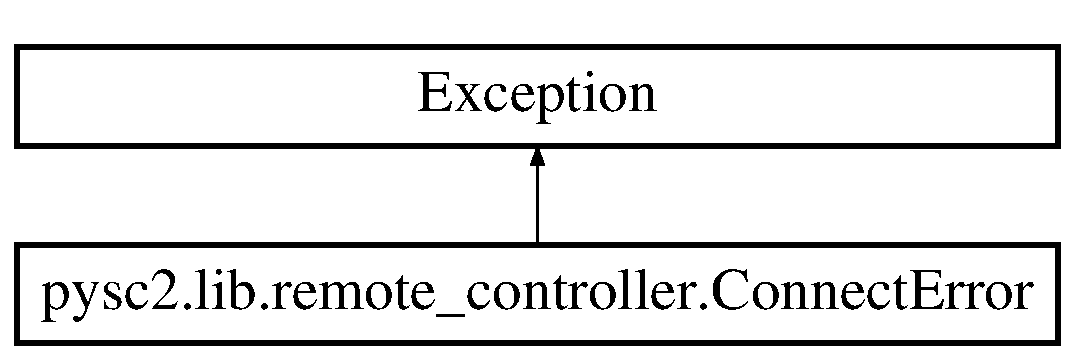
\includegraphics[height=2.000000cm]{classpysc2_1_1lib_1_1remote__controller_1_1_connect_error}
\end{center}
\end{figure}


The documentation for this class was generated from the following file\+:\begin{DoxyCompactItemize}
\item 
lib/\mbox{\hyperlink{remote__controller_8py}{remote\+\_\+controller.\+py}}\end{DoxyCompactItemize}

\hypertarget{classpysc2_1_1lib_1_1protocol_1_1_connection_error}{}\section{pysc2.\+lib.\+protocol.\+Connection\+Error Class Reference}
\label{classpysc2_1_1lib_1_1protocol_1_1_connection_error}\index{pysc2.\+lib.\+protocol.\+Connection\+Error@{pysc2.\+lib.\+protocol.\+Connection\+Error}}
Inheritance diagram for pysc2.\+lib.\+protocol.\+Connection\+Error\+:\begin{figure}[H]
\begin{center}
\leavevmode
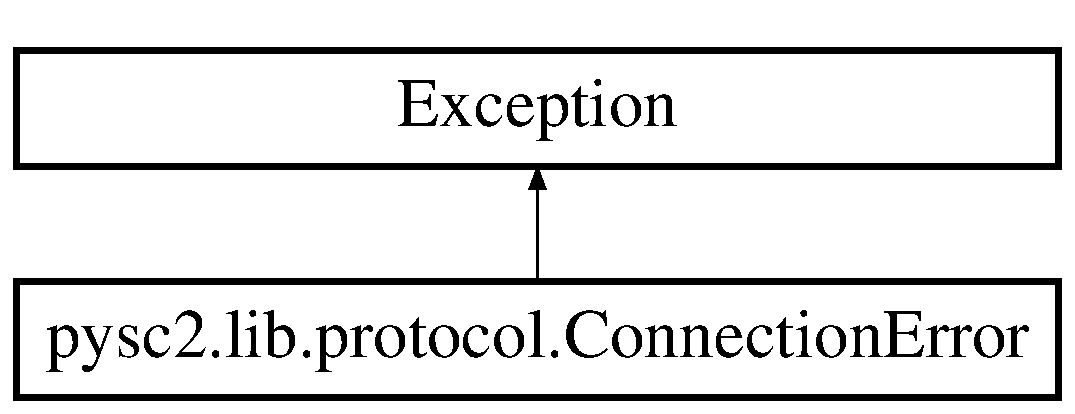
\includegraphics[height=2.000000cm]{classpysc2_1_1lib_1_1protocol_1_1_connection_error}
\end{center}
\end{figure}


\subsection{Detailed Description}
\begin{DoxyVerb}Failed to read/write a message, details in the error string.\end{DoxyVerb}
 

The documentation for this class was generated from the following file\+:\begin{DoxyCompactItemize}
\item 
lib/\mbox{\hyperlink{protocol_8py}{protocol.\+py}}\end{DoxyCompactItemize}

\hypertarget{classpysc2_1_1run__configs_1_1platforms_1_1_cygwin}{}\section{pysc2.\+run\+\_\+configs.\+platforms.\+Cygwin Class Reference}
\label{classpysc2_1_1run__configs_1_1platforms_1_1_cygwin}\index{pysc2.\+run\+\_\+configs.\+platforms.\+Cygwin@{pysc2.\+run\+\_\+configs.\+platforms.\+Cygwin}}
Inheritance diagram for pysc2.\+run\+\_\+configs.\+platforms.\+Cygwin\+:\begin{figure}[H]
\begin{center}
\leavevmode
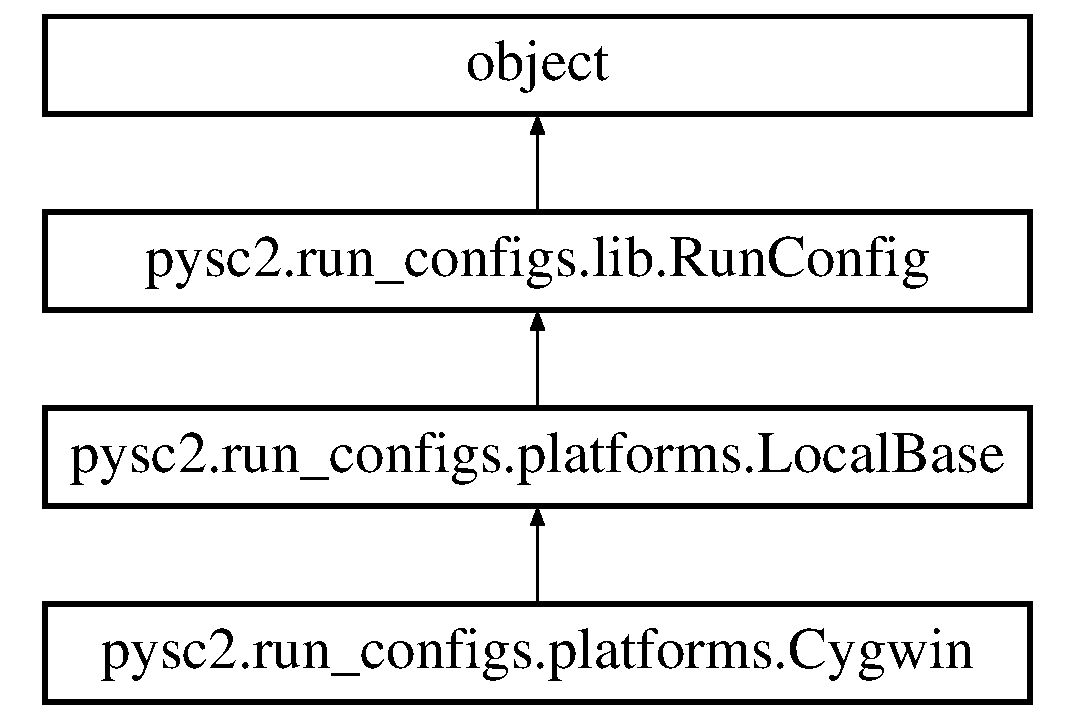
\includegraphics[height=4.000000cm]{classpysc2_1_1run__configs_1_1platforms_1_1_cygwin}
\end{center}
\end{figure}
\subsection*{Public Member Functions}
\begin{DoxyCompactItemize}
\item 
def \mbox{\hyperlink{classpysc2_1_1run__configs_1_1platforms_1_1_cygwin_a937136aea31d51f916be605e608bade0}{\+\_\+\+\_\+init\+\_\+\+\_\+}} (self)
\item 
def \mbox{\hyperlink{classpysc2_1_1run__configs_1_1platforms_1_1_cygwin_ad4c0c92b689396b1ed9759ba69cdc0c6}{priority}} (cls)
\end{DoxyCompactItemize}
\subsection*{Additional Inherited Members}


\subsection{Detailed Description}
\begin{DoxyVerb}Run on Cygwin. This runs the windows binary within a cygwin terminal.\end{DoxyVerb}
 

\subsection{Constructor \& Destructor Documentation}
\mbox{\Hypertarget{classpysc2_1_1run__configs_1_1platforms_1_1_cygwin_a937136aea31d51f916be605e608bade0}\label{classpysc2_1_1run__configs_1_1platforms_1_1_cygwin_a937136aea31d51f916be605e608bade0}} 
\index{pysc2\+::run\+\_\+configs\+::platforms\+::\+Cygwin@{pysc2\+::run\+\_\+configs\+::platforms\+::\+Cygwin}!\+\_\+\+\_\+init\+\_\+\+\_\+@{\+\_\+\+\_\+init\+\_\+\+\_\+}}
\index{\+\_\+\+\_\+init\+\_\+\+\_\+@{\+\_\+\+\_\+init\+\_\+\+\_\+}!pysc2\+::run\+\_\+configs\+::platforms\+::\+Cygwin@{pysc2\+::run\+\_\+configs\+::platforms\+::\+Cygwin}}
\subsubsection{\texorpdfstring{\+\_\+\+\_\+init\+\_\+\+\_\+()}{\_\_init\_\_()}}
{\footnotesize\ttfamily def pysc2.\+run\+\_\+configs.\+platforms.\+Cygwin.\+\_\+\+\_\+init\+\_\+\+\_\+ (\begin{DoxyParamCaption}\item[{}]{self }\end{DoxyParamCaption})}



\subsection{Member Function Documentation}
\mbox{\Hypertarget{classpysc2_1_1run__configs_1_1platforms_1_1_cygwin_ad4c0c92b689396b1ed9759ba69cdc0c6}\label{classpysc2_1_1run__configs_1_1platforms_1_1_cygwin_ad4c0c92b689396b1ed9759ba69cdc0c6}} 
\index{pysc2\+::run\+\_\+configs\+::platforms\+::\+Cygwin@{pysc2\+::run\+\_\+configs\+::platforms\+::\+Cygwin}!priority@{priority}}
\index{priority@{priority}!pysc2\+::run\+\_\+configs\+::platforms\+::\+Cygwin@{pysc2\+::run\+\_\+configs\+::platforms\+::\+Cygwin}}
\subsubsection{\texorpdfstring{priority()}{priority()}}
{\footnotesize\ttfamily def pysc2.\+run\+\_\+configs.\+platforms.\+Cygwin.\+priority (\begin{DoxyParamCaption}\item[{}]{cls }\end{DoxyParamCaption})}



The documentation for this class was generated from the following file\+:\begin{DoxyCompactItemize}
\item 
run\+\_\+configs/\mbox{\hyperlink{platforms_8py}{platforms.\+py}}\end{DoxyCompactItemize}

\hypertarget{classpysc2_1_1agents_1_1scripted__agent_1_1_defeat_roaches}{}\section{pysc2.\+agents.\+scripted\+\_\+agent.\+Defeat\+Roaches Class Reference}
\label{classpysc2_1_1agents_1_1scripted__agent_1_1_defeat_roaches}\index{pysc2.\+agents.\+scripted\+\_\+agent.\+Defeat\+Roaches@{pysc2.\+agents.\+scripted\+\_\+agent.\+Defeat\+Roaches}}
Inheritance diagram for pysc2.\+agents.\+scripted\+\_\+agent.\+Defeat\+Roaches\+:\begin{figure}[H]
\begin{center}
\leavevmode
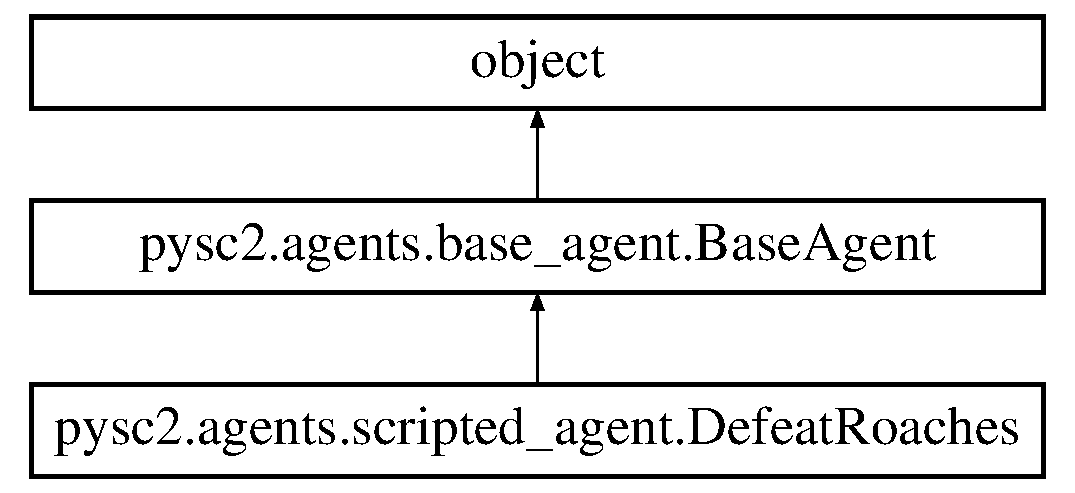
\includegraphics[height=3.000000cm]{classpysc2_1_1agents_1_1scripted__agent_1_1_defeat_roaches}
\end{center}
\end{figure}
\subsection*{Public Member Functions}
\begin{DoxyCompactItemize}
\item 
def \mbox{\hyperlink{classpysc2_1_1agents_1_1scripted__agent_1_1_defeat_roaches_a681a94d365c4725ba8fa30bbc682e4ac}{step}} (self, obs)
\end{DoxyCompactItemize}
\subsection*{Additional Inherited Members}


\subsection{Detailed Description}
\begin{DoxyVerb}An agent specifically for solving the DefeatRoaches map.\end{DoxyVerb}
 

\subsection{Member Function Documentation}
\mbox{\Hypertarget{classpysc2_1_1agents_1_1scripted__agent_1_1_defeat_roaches_a681a94d365c4725ba8fa30bbc682e4ac}\label{classpysc2_1_1agents_1_1scripted__agent_1_1_defeat_roaches_a681a94d365c4725ba8fa30bbc682e4ac}} 
\index{pysc2\+::agents\+::scripted\+\_\+agent\+::\+Defeat\+Roaches@{pysc2\+::agents\+::scripted\+\_\+agent\+::\+Defeat\+Roaches}!step@{step}}
\index{step@{step}!pysc2\+::agents\+::scripted\+\_\+agent\+::\+Defeat\+Roaches@{pysc2\+::agents\+::scripted\+\_\+agent\+::\+Defeat\+Roaches}}
\subsubsection{\texorpdfstring{step()}{step()}}
{\footnotesize\ttfamily def pysc2.\+agents.\+scripted\+\_\+agent.\+Defeat\+Roaches.\+step (\begin{DoxyParamCaption}\item[{}]{self,  }\item[{}]{obs }\end{DoxyParamCaption})}



The documentation for this class was generated from the following file\+:\begin{DoxyCompactItemize}
\item 
agents/\mbox{\hyperlink{scripted__agent_8py}{scripted\+\_\+agent.\+py}}\end{DoxyCompactItemize}

\hypertarget{classpysc2_1_1env_1_1sc2__env_1_1_difficulty}{}\section{pysc2.\+env.\+sc2\+\_\+env.\+Difficulty Class Reference}
\label{classpysc2_1_1env_1_1sc2__env_1_1_difficulty}\index{pysc2.\+env.\+sc2\+\_\+env.\+Difficulty@{pysc2.\+env.\+sc2\+\_\+env.\+Difficulty}}
Inheritance diagram for pysc2.\+env.\+sc2\+\_\+env.\+Difficulty\+:\begin{figure}[H]
\begin{center}
\leavevmode
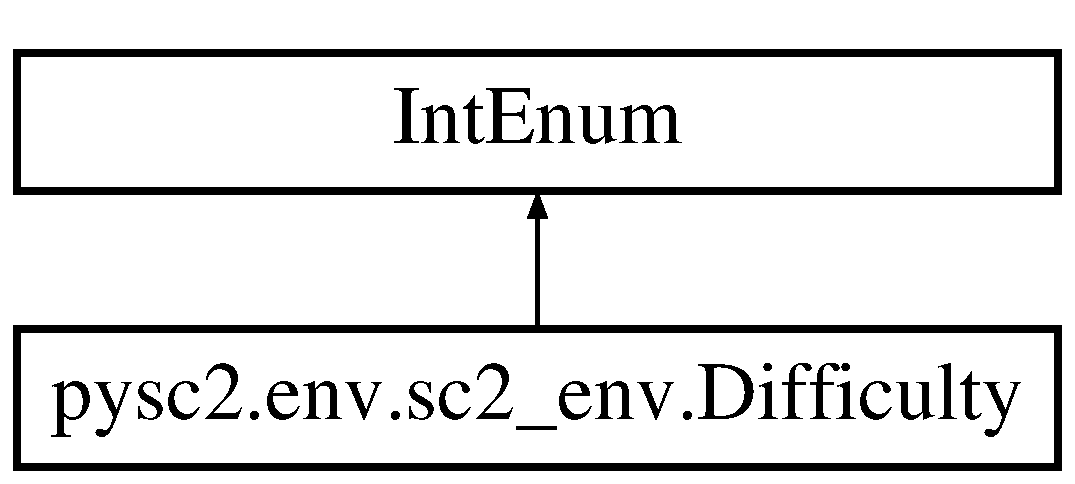
\includegraphics[height=2.000000cm]{classpysc2_1_1env_1_1sc2__env_1_1_difficulty}
\end{center}
\end{figure}
\subsection*{Static Public Attributes}
\begin{DoxyCompactItemize}
\item 
\mbox{\hyperlink{classpysc2_1_1env_1_1sc2__env_1_1_difficulty_ad18cddab1aeb3e4bfa8e5d053db9cc7a}{very\+\_\+easy}} = sc\+\_\+pb.\+Very\+Easy
\item 
\mbox{\hyperlink{classpysc2_1_1env_1_1sc2__env_1_1_difficulty_a91ae2b79485f42d369c2188187818e85}{easy}} = sc\+\_\+pb.\+Easy
\item 
\mbox{\hyperlink{classpysc2_1_1env_1_1sc2__env_1_1_difficulty_a706a666a3a2e916bfefdcd0dd57ff6ae}{medium}} = sc\+\_\+pb.\+Medium
\item 
\mbox{\hyperlink{classpysc2_1_1env_1_1sc2__env_1_1_difficulty_af78449b9e9abe19205a4b318265da564}{medium\+\_\+hard}} = sc\+\_\+pb.\+Medium\+Hard
\item 
\mbox{\hyperlink{classpysc2_1_1env_1_1sc2__env_1_1_difficulty_abaa3239dd900a199541dfe84245615bc}{hard}} = sc\+\_\+pb.\+Hard
\item 
\mbox{\hyperlink{classpysc2_1_1env_1_1sc2__env_1_1_difficulty_a5993c03de5b86b5da9d6c2c651df1132}{harder}} = sc\+\_\+pb.\+Harder
\item 
\mbox{\hyperlink{classpysc2_1_1env_1_1sc2__env_1_1_difficulty_a9d4a5c2e15f804b56949a6bc72c973b1}{very\+\_\+hard}} = sc\+\_\+pb.\+Very\+Hard
\item 
\mbox{\hyperlink{classpysc2_1_1env_1_1sc2__env_1_1_difficulty_a8e11dd0c16f631023aec02f99d414a12}{cheat\+\_\+vision}} = sc\+\_\+pb.\+Cheat\+Vision
\item 
\mbox{\hyperlink{classpysc2_1_1env_1_1sc2__env_1_1_difficulty_a982b1d88aef08815c846126ce7319be0}{cheat\+\_\+money}} = sc\+\_\+pb.\+Cheat\+Money
\item 
\mbox{\hyperlink{classpysc2_1_1env_1_1sc2__env_1_1_difficulty_a9e46cdfe4b569bccdfb8cea96e95d1a4}{cheat\+\_\+insane}} = sc\+\_\+pb.\+Cheat\+Insane
\end{DoxyCompactItemize}


\subsection{Detailed Description}
\begin{DoxyVerb}Bot difficulties.\end{DoxyVerb}
 

\subsection{Member Data Documentation}
\mbox{\Hypertarget{classpysc2_1_1env_1_1sc2__env_1_1_difficulty_a9e46cdfe4b569bccdfb8cea96e95d1a4}\label{classpysc2_1_1env_1_1sc2__env_1_1_difficulty_a9e46cdfe4b569bccdfb8cea96e95d1a4}} 
\index{pysc2\+::env\+::sc2\+\_\+env\+::\+Difficulty@{pysc2\+::env\+::sc2\+\_\+env\+::\+Difficulty}!cheat\+\_\+insane@{cheat\+\_\+insane}}
\index{cheat\+\_\+insane@{cheat\+\_\+insane}!pysc2\+::env\+::sc2\+\_\+env\+::\+Difficulty@{pysc2\+::env\+::sc2\+\_\+env\+::\+Difficulty}}
\subsubsection{\texorpdfstring{cheat\+\_\+insane}{cheat\_insane}}
{\footnotesize\ttfamily pysc2.\+env.\+sc2\+\_\+env.\+Difficulty.\+cheat\+\_\+insane = sc\+\_\+pb.\+Cheat\+Insane\hspace{0.3cm}{\ttfamily [static]}}

\mbox{\Hypertarget{classpysc2_1_1env_1_1sc2__env_1_1_difficulty_a982b1d88aef08815c846126ce7319be0}\label{classpysc2_1_1env_1_1sc2__env_1_1_difficulty_a982b1d88aef08815c846126ce7319be0}} 
\index{pysc2\+::env\+::sc2\+\_\+env\+::\+Difficulty@{pysc2\+::env\+::sc2\+\_\+env\+::\+Difficulty}!cheat\+\_\+money@{cheat\+\_\+money}}
\index{cheat\+\_\+money@{cheat\+\_\+money}!pysc2\+::env\+::sc2\+\_\+env\+::\+Difficulty@{pysc2\+::env\+::sc2\+\_\+env\+::\+Difficulty}}
\subsubsection{\texorpdfstring{cheat\+\_\+money}{cheat\_money}}
{\footnotesize\ttfamily pysc2.\+env.\+sc2\+\_\+env.\+Difficulty.\+cheat\+\_\+money = sc\+\_\+pb.\+Cheat\+Money\hspace{0.3cm}{\ttfamily [static]}}

\mbox{\Hypertarget{classpysc2_1_1env_1_1sc2__env_1_1_difficulty_a8e11dd0c16f631023aec02f99d414a12}\label{classpysc2_1_1env_1_1sc2__env_1_1_difficulty_a8e11dd0c16f631023aec02f99d414a12}} 
\index{pysc2\+::env\+::sc2\+\_\+env\+::\+Difficulty@{pysc2\+::env\+::sc2\+\_\+env\+::\+Difficulty}!cheat\+\_\+vision@{cheat\+\_\+vision}}
\index{cheat\+\_\+vision@{cheat\+\_\+vision}!pysc2\+::env\+::sc2\+\_\+env\+::\+Difficulty@{pysc2\+::env\+::sc2\+\_\+env\+::\+Difficulty}}
\subsubsection{\texorpdfstring{cheat\+\_\+vision}{cheat\_vision}}
{\footnotesize\ttfamily pysc2.\+env.\+sc2\+\_\+env.\+Difficulty.\+cheat\+\_\+vision = sc\+\_\+pb.\+Cheat\+Vision\hspace{0.3cm}{\ttfamily [static]}}

\mbox{\Hypertarget{classpysc2_1_1env_1_1sc2__env_1_1_difficulty_a91ae2b79485f42d369c2188187818e85}\label{classpysc2_1_1env_1_1sc2__env_1_1_difficulty_a91ae2b79485f42d369c2188187818e85}} 
\index{pysc2\+::env\+::sc2\+\_\+env\+::\+Difficulty@{pysc2\+::env\+::sc2\+\_\+env\+::\+Difficulty}!easy@{easy}}
\index{easy@{easy}!pysc2\+::env\+::sc2\+\_\+env\+::\+Difficulty@{pysc2\+::env\+::sc2\+\_\+env\+::\+Difficulty}}
\subsubsection{\texorpdfstring{easy}{easy}}
{\footnotesize\ttfamily pysc2.\+env.\+sc2\+\_\+env.\+Difficulty.\+easy = sc\+\_\+pb.\+Easy\hspace{0.3cm}{\ttfamily [static]}}

\mbox{\Hypertarget{classpysc2_1_1env_1_1sc2__env_1_1_difficulty_abaa3239dd900a199541dfe84245615bc}\label{classpysc2_1_1env_1_1sc2__env_1_1_difficulty_abaa3239dd900a199541dfe84245615bc}} 
\index{pysc2\+::env\+::sc2\+\_\+env\+::\+Difficulty@{pysc2\+::env\+::sc2\+\_\+env\+::\+Difficulty}!hard@{hard}}
\index{hard@{hard}!pysc2\+::env\+::sc2\+\_\+env\+::\+Difficulty@{pysc2\+::env\+::sc2\+\_\+env\+::\+Difficulty}}
\subsubsection{\texorpdfstring{hard}{hard}}
{\footnotesize\ttfamily pysc2.\+env.\+sc2\+\_\+env.\+Difficulty.\+hard = sc\+\_\+pb.\+Hard\hspace{0.3cm}{\ttfamily [static]}}

\mbox{\Hypertarget{classpysc2_1_1env_1_1sc2__env_1_1_difficulty_a5993c03de5b86b5da9d6c2c651df1132}\label{classpysc2_1_1env_1_1sc2__env_1_1_difficulty_a5993c03de5b86b5da9d6c2c651df1132}} 
\index{pysc2\+::env\+::sc2\+\_\+env\+::\+Difficulty@{pysc2\+::env\+::sc2\+\_\+env\+::\+Difficulty}!harder@{harder}}
\index{harder@{harder}!pysc2\+::env\+::sc2\+\_\+env\+::\+Difficulty@{pysc2\+::env\+::sc2\+\_\+env\+::\+Difficulty}}
\subsubsection{\texorpdfstring{harder}{harder}}
{\footnotesize\ttfamily pysc2.\+env.\+sc2\+\_\+env.\+Difficulty.\+harder = sc\+\_\+pb.\+Harder\hspace{0.3cm}{\ttfamily [static]}}

\mbox{\Hypertarget{classpysc2_1_1env_1_1sc2__env_1_1_difficulty_a706a666a3a2e916bfefdcd0dd57ff6ae}\label{classpysc2_1_1env_1_1sc2__env_1_1_difficulty_a706a666a3a2e916bfefdcd0dd57ff6ae}} 
\index{pysc2\+::env\+::sc2\+\_\+env\+::\+Difficulty@{pysc2\+::env\+::sc2\+\_\+env\+::\+Difficulty}!medium@{medium}}
\index{medium@{medium}!pysc2\+::env\+::sc2\+\_\+env\+::\+Difficulty@{pysc2\+::env\+::sc2\+\_\+env\+::\+Difficulty}}
\subsubsection{\texorpdfstring{medium}{medium}}
{\footnotesize\ttfamily pysc2.\+env.\+sc2\+\_\+env.\+Difficulty.\+medium = sc\+\_\+pb.\+Medium\hspace{0.3cm}{\ttfamily [static]}}

\mbox{\Hypertarget{classpysc2_1_1env_1_1sc2__env_1_1_difficulty_af78449b9e9abe19205a4b318265da564}\label{classpysc2_1_1env_1_1sc2__env_1_1_difficulty_af78449b9e9abe19205a4b318265da564}} 
\index{pysc2\+::env\+::sc2\+\_\+env\+::\+Difficulty@{pysc2\+::env\+::sc2\+\_\+env\+::\+Difficulty}!medium\+\_\+hard@{medium\+\_\+hard}}
\index{medium\+\_\+hard@{medium\+\_\+hard}!pysc2\+::env\+::sc2\+\_\+env\+::\+Difficulty@{pysc2\+::env\+::sc2\+\_\+env\+::\+Difficulty}}
\subsubsection{\texorpdfstring{medium\+\_\+hard}{medium\_hard}}
{\footnotesize\ttfamily pysc2.\+env.\+sc2\+\_\+env.\+Difficulty.\+medium\+\_\+hard = sc\+\_\+pb.\+Medium\+Hard\hspace{0.3cm}{\ttfamily [static]}}

\mbox{\Hypertarget{classpysc2_1_1env_1_1sc2__env_1_1_difficulty_ad18cddab1aeb3e4bfa8e5d053db9cc7a}\label{classpysc2_1_1env_1_1sc2__env_1_1_difficulty_ad18cddab1aeb3e4bfa8e5d053db9cc7a}} 
\index{pysc2\+::env\+::sc2\+\_\+env\+::\+Difficulty@{pysc2\+::env\+::sc2\+\_\+env\+::\+Difficulty}!very\+\_\+easy@{very\+\_\+easy}}
\index{very\+\_\+easy@{very\+\_\+easy}!pysc2\+::env\+::sc2\+\_\+env\+::\+Difficulty@{pysc2\+::env\+::sc2\+\_\+env\+::\+Difficulty}}
\subsubsection{\texorpdfstring{very\+\_\+easy}{very\_easy}}
{\footnotesize\ttfamily pysc2.\+env.\+sc2\+\_\+env.\+Difficulty.\+very\+\_\+easy = sc\+\_\+pb.\+Very\+Easy\hspace{0.3cm}{\ttfamily [static]}}

\mbox{\Hypertarget{classpysc2_1_1env_1_1sc2__env_1_1_difficulty_a9d4a5c2e15f804b56949a6bc72c973b1}\label{classpysc2_1_1env_1_1sc2__env_1_1_difficulty_a9d4a5c2e15f804b56949a6bc72c973b1}} 
\index{pysc2\+::env\+::sc2\+\_\+env\+::\+Difficulty@{pysc2\+::env\+::sc2\+\_\+env\+::\+Difficulty}!very\+\_\+hard@{very\+\_\+hard}}
\index{very\+\_\+hard@{very\+\_\+hard}!pysc2\+::env\+::sc2\+\_\+env\+::\+Difficulty@{pysc2\+::env\+::sc2\+\_\+env\+::\+Difficulty}}
\subsubsection{\texorpdfstring{very\+\_\+hard}{very\_hard}}
{\footnotesize\ttfamily pysc2.\+env.\+sc2\+\_\+env.\+Difficulty.\+very\+\_\+hard = sc\+\_\+pb.\+Very\+Hard\hspace{0.3cm}{\ttfamily [static]}}



The documentation for this class was generated from the following file\+:\begin{DoxyCompactItemize}
\item 
env/\mbox{\hyperlink{sc2__env_8py}{sc2\+\_\+env.\+py}}\end{DoxyCompactItemize}

\hypertarget{classpysc2_1_1lib_1_1features_1_1_dimensions}{}\section{pysc2.\+lib.\+features.\+Dimensions Class Reference}
\label{classpysc2_1_1lib_1_1features_1_1_dimensions}\index{pysc2.\+lib.\+features.\+Dimensions@{pysc2.\+lib.\+features.\+Dimensions}}
Inheritance diagram for pysc2.\+lib.\+features.\+Dimensions\+:\begin{figure}[H]
\begin{center}
\leavevmode
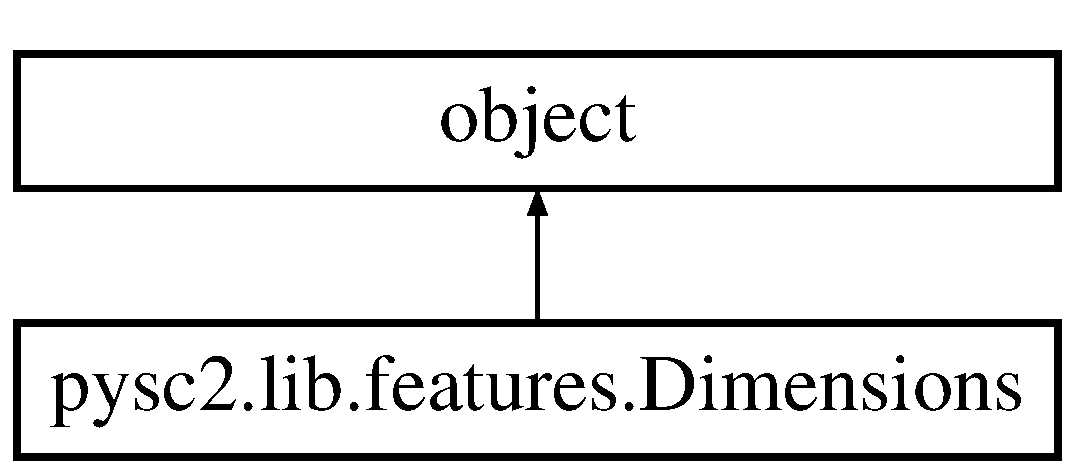
\includegraphics[height=2.000000cm]{classpysc2_1_1lib_1_1features_1_1_dimensions}
\end{center}
\end{figure}
\subsection*{Public Member Functions}
\begin{DoxyCompactItemize}
\item 
def \mbox{\hyperlink{classpysc2_1_1lib_1_1features_1_1_dimensions_a1baec57f9a7f019d9c9147e10473a15e}{\+\_\+\+\_\+init\+\_\+\+\_\+}} (self, \mbox{\hyperlink{classpysc2_1_1lib_1_1features_1_1_dimensions_a8f2a12331c6acb2070a3cd77ce4019f0}{screen}}=None, \mbox{\hyperlink{classpysc2_1_1lib_1_1features_1_1_dimensions_ac3367e0b221b72b66beb5f5b1d5a1169}{minimap}}=None)
\item 
def \mbox{\hyperlink{classpysc2_1_1lib_1_1features_1_1_dimensions_a8f2a12331c6acb2070a3cd77ce4019f0}{screen}} (self)
\item 
def \mbox{\hyperlink{classpysc2_1_1lib_1_1features_1_1_dimensions_ac3367e0b221b72b66beb5f5b1d5a1169}{minimap}} (self)
\item 
def \mbox{\hyperlink{classpysc2_1_1lib_1_1features_1_1_dimensions_a8e72e9bec4a76d1f91ecdf0523991cae}{\+\_\+\+\_\+repr\+\_\+\+\_\+}} (self)
\end{DoxyCompactItemize}


\subsection{Detailed Description}
\begin{DoxyVerb}Screen and minimap dimensions configuration.

Both screen and minimap must be specified. Sizes must be positive.
Screen size must be greater than or equal to minimap size in both dimensions.

Args:
  screen: A (width, height) int tuple or a single int to be used for both.
  minimap: A (width, height) int tuple or a single int to be used for both.
\end{DoxyVerb}
 

\subsection{Constructor \& Destructor Documentation}
\mbox{\Hypertarget{classpysc2_1_1lib_1_1features_1_1_dimensions_a1baec57f9a7f019d9c9147e10473a15e}\label{classpysc2_1_1lib_1_1features_1_1_dimensions_a1baec57f9a7f019d9c9147e10473a15e}} 
\index{pysc2\+::lib\+::features\+::\+Dimensions@{pysc2\+::lib\+::features\+::\+Dimensions}!\+\_\+\+\_\+init\+\_\+\+\_\+@{\+\_\+\+\_\+init\+\_\+\+\_\+}}
\index{\+\_\+\+\_\+init\+\_\+\+\_\+@{\+\_\+\+\_\+init\+\_\+\+\_\+}!pysc2\+::lib\+::features\+::\+Dimensions@{pysc2\+::lib\+::features\+::\+Dimensions}}
\subsubsection{\texorpdfstring{\+\_\+\+\_\+init\+\_\+\+\_\+()}{\_\_init\_\_()}}
{\footnotesize\ttfamily def pysc2.\+lib.\+features.\+Dimensions.\+\_\+\+\_\+init\+\_\+\+\_\+ (\begin{DoxyParamCaption}\item[{}]{self,  }\item[{}]{screen = {\ttfamily None},  }\item[{}]{minimap = {\ttfamily None} }\end{DoxyParamCaption})}



\subsection{Member Function Documentation}
\mbox{\Hypertarget{classpysc2_1_1lib_1_1features_1_1_dimensions_a8e72e9bec4a76d1f91ecdf0523991cae}\label{classpysc2_1_1lib_1_1features_1_1_dimensions_a8e72e9bec4a76d1f91ecdf0523991cae}} 
\index{pysc2\+::lib\+::features\+::\+Dimensions@{pysc2\+::lib\+::features\+::\+Dimensions}!\+\_\+\+\_\+repr\+\_\+\+\_\+@{\+\_\+\+\_\+repr\+\_\+\+\_\+}}
\index{\+\_\+\+\_\+repr\+\_\+\+\_\+@{\+\_\+\+\_\+repr\+\_\+\+\_\+}!pysc2\+::lib\+::features\+::\+Dimensions@{pysc2\+::lib\+::features\+::\+Dimensions}}
\subsubsection{\texorpdfstring{\+\_\+\+\_\+repr\+\_\+\+\_\+()}{\_\_repr\_\_()}}
{\footnotesize\ttfamily def pysc2.\+lib.\+features.\+Dimensions.\+\_\+\+\_\+repr\+\_\+\+\_\+ (\begin{DoxyParamCaption}\item[{}]{self }\end{DoxyParamCaption})}

\mbox{\Hypertarget{classpysc2_1_1lib_1_1features_1_1_dimensions_ac3367e0b221b72b66beb5f5b1d5a1169}\label{classpysc2_1_1lib_1_1features_1_1_dimensions_ac3367e0b221b72b66beb5f5b1d5a1169}} 
\index{pysc2\+::lib\+::features\+::\+Dimensions@{pysc2\+::lib\+::features\+::\+Dimensions}!minimap@{minimap}}
\index{minimap@{minimap}!pysc2\+::lib\+::features\+::\+Dimensions@{pysc2\+::lib\+::features\+::\+Dimensions}}
\subsubsection{\texorpdfstring{minimap()}{minimap()}}
{\footnotesize\ttfamily def pysc2.\+lib.\+features.\+Dimensions.\+minimap (\begin{DoxyParamCaption}\item[{}]{self }\end{DoxyParamCaption})}

\mbox{\Hypertarget{classpysc2_1_1lib_1_1features_1_1_dimensions_a8f2a12331c6acb2070a3cd77ce4019f0}\label{classpysc2_1_1lib_1_1features_1_1_dimensions_a8f2a12331c6acb2070a3cd77ce4019f0}} 
\index{pysc2\+::lib\+::features\+::\+Dimensions@{pysc2\+::lib\+::features\+::\+Dimensions}!screen@{screen}}
\index{screen@{screen}!pysc2\+::lib\+::features\+::\+Dimensions@{pysc2\+::lib\+::features\+::\+Dimensions}}
\subsubsection{\texorpdfstring{screen()}{screen()}}
{\footnotesize\ttfamily def pysc2.\+lib.\+features.\+Dimensions.\+screen (\begin{DoxyParamCaption}\item[{}]{self }\end{DoxyParamCaption})}



The documentation for this class was generated from the following file\+:\begin{DoxyCompactItemize}
\item 
lib/\mbox{\hyperlink{features_8py}{features.\+py}}\end{DoxyCompactItemize}

\hypertarget{classpysc2_1_1lib_1_1features__test_1_1_dimensions_test}{}\section{pysc2.\+lib.\+features\+\_\+test.\+Dimensions\+Test Class Reference}
\label{classpysc2_1_1lib_1_1features__test_1_1_dimensions_test}\index{pysc2.\+lib.\+features\+\_\+test.\+Dimensions\+Test@{pysc2.\+lib.\+features\+\_\+test.\+Dimensions\+Test}}
Inheritance diagram for pysc2.\+lib.\+features\+\_\+test.\+Dimensions\+Test\+:\begin{figure}[H]
\begin{center}
\leavevmode
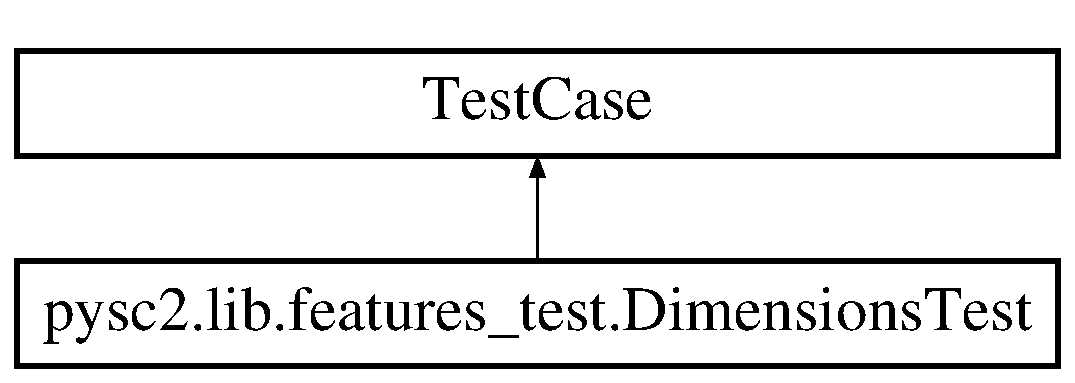
\includegraphics[height=2.000000cm]{classpysc2_1_1lib_1_1features__test_1_1_dimensions_test}
\end{center}
\end{figure}
\subsection*{Public Member Functions}
\begin{DoxyCompactItemize}
\item 
def \mbox{\hyperlink{classpysc2_1_1lib_1_1features__test_1_1_dimensions_test_a656658d118ecf0dec068a5f1f840480a}{test\+Screen\+Size\+Without\+Minimap\+Raises}} (self)
\item 
def \mbox{\hyperlink{classpysc2_1_1lib_1_1features__test_1_1_dimensions_test_a5d54ae68a70ede7e77ebc5a82f9bb363}{test\+Screen\+Width\+Without\+Height\+Raises}} (self)
\item 
def \mbox{\hyperlink{classpysc2_1_1lib_1_1features__test_1_1_dimensions_test_a98381d48e02f0575e16df437120ad0b6}{test\+Screen\+Width\+Height\+Without\+Minimap\+Raises}} (self)
\item 
def \mbox{\hyperlink{classpysc2_1_1lib_1_1features__test_1_1_dimensions_test_a477eb9b53b64219aa10f5460a1e2735a}{test\+Minimap\+Width\+And\+Height\+Without\+Screen\+Raises}} (self)
\item 
def \mbox{\hyperlink{classpysc2_1_1lib_1_1features__test_1_1_dimensions_test_af6f69ee9ae5eb17bc7e324caa7add776}{test\+Screen\+Smaller\+Than\+Minimap\+Raises}} (self)
\item 
def \mbox{\hyperlink{classpysc2_1_1lib_1_1features__test_1_1_dimensions_test_a68a0e81f9af4953ef8e51e2376296c86}{test\+None\+None\+Raises}} (self)
\item 
def \mbox{\hyperlink{classpysc2_1_1lib_1_1features__test_1_1_dimensions_test_a715543385b64f77ed16e6370fbba56fd}{test\+Singular\+Zeroes\+Raises}} (self)
\item 
def \mbox{\hyperlink{classpysc2_1_1lib_1_1features__test_1_1_dimensions_test_a415323bb2471aecc5255d210cbd99801}{test\+Two\+Zeroes\+Raises}} (self)
\item 
def \mbox{\hyperlink{classpysc2_1_1lib_1_1features__test_1_1_dimensions_test_a43f03496b5f601bfcd4a2b43d16bd165}{test\+Three\+Tuple\+Screen\+Raises}} (self)
\item 
def \mbox{\hyperlink{classpysc2_1_1lib_1_1features__test_1_1_dimensions_test_a9bf1bf5fd35bf14528343c64e92cfa3e}{test\+Three\+Tuple\+Minimap\+Raises}} (self)
\item 
def \mbox{\hyperlink{classpysc2_1_1lib_1_1features__test_1_1_dimensions_test_a6818938975cbcea85dcc17ee1d506053}{test\+Negative\+Screen\+Raises}} (self)
\item 
def \mbox{\hyperlink{classpysc2_1_1lib_1_1features__test_1_1_dimensions_test_a689adbba28df393a9b16b36413b08d29}{test\+Negative\+Minimap\+Raises}} (self)
\item 
def \mbox{\hyperlink{classpysc2_1_1lib_1_1features__test_1_1_dimensions_test_a4fa9ba1d024fbee643cca67ed215627d}{test\+Negative\+Screen\+Tuple\+Raises}} (self)
\item 
def \mbox{\hyperlink{classpysc2_1_1lib_1_1features__test_1_1_dimensions_test_ac762a20913b445f3137cf72191edff70}{test\+Negative\+Minimap\+Tuple\+Raises}} (self)
\end{DoxyCompactItemize}


\subsection{Member Function Documentation}
\mbox{\Hypertarget{classpysc2_1_1lib_1_1features__test_1_1_dimensions_test_a477eb9b53b64219aa10f5460a1e2735a}\label{classpysc2_1_1lib_1_1features__test_1_1_dimensions_test_a477eb9b53b64219aa10f5460a1e2735a}} 
\index{pysc2\+::lib\+::features\+\_\+test\+::\+Dimensions\+Test@{pysc2\+::lib\+::features\+\_\+test\+::\+Dimensions\+Test}!test\+Minimap\+Width\+And\+Height\+Without\+Screen\+Raises@{test\+Minimap\+Width\+And\+Height\+Without\+Screen\+Raises}}
\index{test\+Minimap\+Width\+And\+Height\+Without\+Screen\+Raises@{test\+Minimap\+Width\+And\+Height\+Without\+Screen\+Raises}!pysc2\+::lib\+::features\+\_\+test\+::\+Dimensions\+Test@{pysc2\+::lib\+::features\+\_\+test\+::\+Dimensions\+Test}}
\subsubsection{\texorpdfstring{test\+Minimap\+Width\+And\+Height\+Without\+Screen\+Raises()}{testMinimapWidthAndHeightWithoutScreenRaises()}}
{\footnotesize\ttfamily def pysc2.\+lib.\+features\+\_\+test.\+Dimensions\+Test.\+test\+Minimap\+Width\+And\+Height\+Without\+Screen\+Raises (\begin{DoxyParamCaption}\item[{}]{self }\end{DoxyParamCaption})}

\mbox{\Hypertarget{classpysc2_1_1lib_1_1features__test_1_1_dimensions_test_a689adbba28df393a9b16b36413b08d29}\label{classpysc2_1_1lib_1_1features__test_1_1_dimensions_test_a689adbba28df393a9b16b36413b08d29}} 
\index{pysc2\+::lib\+::features\+\_\+test\+::\+Dimensions\+Test@{pysc2\+::lib\+::features\+\_\+test\+::\+Dimensions\+Test}!test\+Negative\+Minimap\+Raises@{test\+Negative\+Minimap\+Raises}}
\index{test\+Negative\+Minimap\+Raises@{test\+Negative\+Minimap\+Raises}!pysc2\+::lib\+::features\+\_\+test\+::\+Dimensions\+Test@{pysc2\+::lib\+::features\+\_\+test\+::\+Dimensions\+Test}}
\subsubsection{\texorpdfstring{test\+Negative\+Minimap\+Raises()}{testNegativeMinimapRaises()}}
{\footnotesize\ttfamily def pysc2.\+lib.\+features\+\_\+test.\+Dimensions\+Test.\+test\+Negative\+Minimap\+Raises (\begin{DoxyParamCaption}\item[{}]{self }\end{DoxyParamCaption})}

\mbox{\Hypertarget{classpysc2_1_1lib_1_1features__test_1_1_dimensions_test_ac762a20913b445f3137cf72191edff70}\label{classpysc2_1_1lib_1_1features__test_1_1_dimensions_test_ac762a20913b445f3137cf72191edff70}} 
\index{pysc2\+::lib\+::features\+\_\+test\+::\+Dimensions\+Test@{pysc2\+::lib\+::features\+\_\+test\+::\+Dimensions\+Test}!test\+Negative\+Minimap\+Tuple\+Raises@{test\+Negative\+Minimap\+Tuple\+Raises}}
\index{test\+Negative\+Minimap\+Tuple\+Raises@{test\+Negative\+Minimap\+Tuple\+Raises}!pysc2\+::lib\+::features\+\_\+test\+::\+Dimensions\+Test@{pysc2\+::lib\+::features\+\_\+test\+::\+Dimensions\+Test}}
\subsubsection{\texorpdfstring{test\+Negative\+Minimap\+Tuple\+Raises()}{testNegativeMinimapTupleRaises()}}
{\footnotesize\ttfamily def pysc2.\+lib.\+features\+\_\+test.\+Dimensions\+Test.\+test\+Negative\+Minimap\+Tuple\+Raises (\begin{DoxyParamCaption}\item[{}]{self }\end{DoxyParamCaption})}

\mbox{\Hypertarget{classpysc2_1_1lib_1_1features__test_1_1_dimensions_test_a6818938975cbcea85dcc17ee1d506053}\label{classpysc2_1_1lib_1_1features__test_1_1_dimensions_test_a6818938975cbcea85dcc17ee1d506053}} 
\index{pysc2\+::lib\+::features\+\_\+test\+::\+Dimensions\+Test@{pysc2\+::lib\+::features\+\_\+test\+::\+Dimensions\+Test}!test\+Negative\+Screen\+Raises@{test\+Negative\+Screen\+Raises}}
\index{test\+Negative\+Screen\+Raises@{test\+Negative\+Screen\+Raises}!pysc2\+::lib\+::features\+\_\+test\+::\+Dimensions\+Test@{pysc2\+::lib\+::features\+\_\+test\+::\+Dimensions\+Test}}
\subsubsection{\texorpdfstring{test\+Negative\+Screen\+Raises()}{testNegativeScreenRaises()}}
{\footnotesize\ttfamily def pysc2.\+lib.\+features\+\_\+test.\+Dimensions\+Test.\+test\+Negative\+Screen\+Raises (\begin{DoxyParamCaption}\item[{}]{self }\end{DoxyParamCaption})}

\mbox{\Hypertarget{classpysc2_1_1lib_1_1features__test_1_1_dimensions_test_a4fa9ba1d024fbee643cca67ed215627d}\label{classpysc2_1_1lib_1_1features__test_1_1_dimensions_test_a4fa9ba1d024fbee643cca67ed215627d}} 
\index{pysc2\+::lib\+::features\+\_\+test\+::\+Dimensions\+Test@{pysc2\+::lib\+::features\+\_\+test\+::\+Dimensions\+Test}!test\+Negative\+Screen\+Tuple\+Raises@{test\+Negative\+Screen\+Tuple\+Raises}}
\index{test\+Negative\+Screen\+Tuple\+Raises@{test\+Negative\+Screen\+Tuple\+Raises}!pysc2\+::lib\+::features\+\_\+test\+::\+Dimensions\+Test@{pysc2\+::lib\+::features\+\_\+test\+::\+Dimensions\+Test}}
\subsubsection{\texorpdfstring{test\+Negative\+Screen\+Tuple\+Raises()}{testNegativeScreenTupleRaises()}}
{\footnotesize\ttfamily def pysc2.\+lib.\+features\+\_\+test.\+Dimensions\+Test.\+test\+Negative\+Screen\+Tuple\+Raises (\begin{DoxyParamCaption}\item[{}]{self }\end{DoxyParamCaption})}

\mbox{\Hypertarget{classpysc2_1_1lib_1_1features__test_1_1_dimensions_test_a68a0e81f9af4953ef8e51e2376296c86}\label{classpysc2_1_1lib_1_1features__test_1_1_dimensions_test_a68a0e81f9af4953ef8e51e2376296c86}} 
\index{pysc2\+::lib\+::features\+\_\+test\+::\+Dimensions\+Test@{pysc2\+::lib\+::features\+\_\+test\+::\+Dimensions\+Test}!test\+None\+None\+Raises@{test\+None\+None\+Raises}}
\index{test\+None\+None\+Raises@{test\+None\+None\+Raises}!pysc2\+::lib\+::features\+\_\+test\+::\+Dimensions\+Test@{pysc2\+::lib\+::features\+\_\+test\+::\+Dimensions\+Test}}
\subsubsection{\texorpdfstring{test\+None\+None\+Raises()}{testNoneNoneRaises()}}
{\footnotesize\ttfamily def pysc2.\+lib.\+features\+\_\+test.\+Dimensions\+Test.\+test\+None\+None\+Raises (\begin{DoxyParamCaption}\item[{}]{self }\end{DoxyParamCaption})}

\mbox{\Hypertarget{classpysc2_1_1lib_1_1features__test_1_1_dimensions_test_a656658d118ecf0dec068a5f1f840480a}\label{classpysc2_1_1lib_1_1features__test_1_1_dimensions_test_a656658d118ecf0dec068a5f1f840480a}} 
\index{pysc2\+::lib\+::features\+\_\+test\+::\+Dimensions\+Test@{pysc2\+::lib\+::features\+\_\+test\+::\+Dimensions\+Test}!test\+Screen\+Size\+Without\+Minimap\+Raises@{test\+Screen\+Size\+Without\+Minimap\+Raises}}
\index{test\+Screen\+Size\+Without\+Minimap\+Raises@{test\+Screen\+Size\+Without\+Minimap\+Raises}!pysc2\+::lib\+::features\+\_\+test\+::\+Dimensions\+Test@{pysc2\+::lib\+::features\+\_\+test\+::\+Dimensions\+Test}}
\subsubsection{\texorpdfstring{test\+Screen\+Size\+Without\+Minimap\+Raises()}{testScreenSizeWithoutMinimapRaises()}}
{\footnotesize\ttfamily def pysc2.\+lib.\+features\+\_\+test.\+Dimensions\+Test.\+test\+Screen\+Size\+Without\+Minimap\+Raises (\begin{DoxyParamCaption}\item[{}]{self }\end{DoxyParamCaption})}

\mbox{\Hypertarget{classpysc2_1_1lib_1_1features__test_1_1_dimensions_test_af6f69ee9ae5eb17bc7e324caa7add776}\label{classpysc2_1_1lib_1_1features__test_1_1_dimensions_test_af6f69ee9ae5eb17bc7e324caa7add776}} 
\index{pysc2\+::lib\+::features\+\_\+test\+::\+Dimensions\+Test@{pysc2\+::lib\+::features\+\_\+test\+::\+Dimensions\+Test}!test\+Screen\+Smaller\+Than\+Minimap\+Raises@{test\+Screen\+Smaller\+Than\+Minimap\+Raises}}
\index{test\+Screen\+Smaller\+Than\+Minimap\+Raises@{test\+Screen\+Smaller\+Than\+Minimap\+Raises}!pysc2\+::lib\+::features\+\_\+test\+::\+Dimensions\+Test@{pysc2\+::lib\+::features\+\_\+test\+::\+Dimensions\+Test}}
\subsubsection{\texorpdfstring{test\+Screen\+Smaller\+Than\+Minimap\+Raises()}{testScreenSmallerThanMinimapRaises()}}
{\footnotesize\ttfamily def pysc2.\+lib.\+features\+\_\+test.\+Dimensions\+Test.\+test\+Screen\+Smaller\+Than\+Minimap\+Raises (\begin{DoxyParamCaption}\item[{}]{self }\end{DoxyParamCaption})}

\mbox{\Hypertarget{classpysc2_1_1lib_1_1features__test_1_1_dimensions_test_a98381d48e02f0575e16df437120ad0b6}\label{classpysc2_1_1lib_1_1features__test_1_1_dimensions_test_a98381d48e02f0575e16df437120ad0b6}} 
\index{pysc2\+::lib\+::features\+\_\+test\+::\+Dimensions\+Test@{pysc2\+::lib\+::features\+\_\+test\+::\+Dimensions\+Test}!test\+Screen\+Width\+Height\+Without\+Minimap\+Raises@{test\+Screen\+Width\+Height\+Without\+Minimap\+Raises}}
\index{test\+Screen\+Width\+Height\+Without\+Minimap\+Raises@{test\+Screen\+Width\+Height\+Without\+Minimap\+Raises}!pysc2\+::lib\+::features\+\_\+test\+::\+Dimensions\+Test@{pysc2\+::lib\+::features\+\_\+test\+::\+Dimensions\+Test}}
\subsubsection{\texorpdfstring{test\+Screen\+Width\+Height\+Without\+Minimap\+Raises()}{testScreenWidthHeightWithoutMinimapRaises()}}
{\footnotesize\ttfamily def pysc2.\+lib.\+features\+\_\+test.\+Dimensions\+Test.\+test\+Screen\+Width\+Height\+Without\+Minimap\+Raises (\begin{DoxyParamCaption}\item[{}]{self }\end{DoxyParamCaption})}

\mbox{\Hypertarget{classpysc2_1_1lib_1_1features__test_1_1_dimensions_test_a5d54ae68a70ede7e77ebc5a82f9bb363}\label{classpysc2_1_1lib_1_1features__test_1_1_dimensions_test_a5d54ae68a70ede7e77ebc5a82f9bb363}} 
\index{pysc2\+::lib\+::features\+\_\+test\+::\+Dimensions\+Test@{pysc2\+::lib\+::features\+\_\+test\+::\+Dimensions\+Test}!test\+Screen\+Width\+Without\+Height\+Raises@{test\+Screen\+Width\+Without\+Height\+Raises}}
\index{test\+Screen\+Width\+Without\+Height\+Raises@{test\+Screen\+Width\+Without\+Height\+Raises}!pysc2\+::lib\+::features\+\_\+test\+::\+Dimensions\+Test@{pysc2\+::lib\+::features\+\_\+test\+::\+Dimensions\+Test}}
\subsubsection{\texorpdfstring{test\+Screen\+Width\+Without\+Height\+Raises()}{testScreenWidthWithoutHeightRaises()}}
{\footnotesize\ttfamily def pysc2.\+lib.\+features\+\_\+test.\+Dimensions\+Test.\+test\+Screen\+Width\+Without\+Height\+Raises (\begin{DoxyParamCaption}\item[{}]{self }\end{DoxyParamCaption})}

\mbox{\Hypertarget{classpysc2_1_1lib_1_1features__test_1_1_dimensions_test_a715543385b64f77ed16e6370fbba56fd}\label{classpysc2_1_1lib_1_1features__test_1_1_dimensions_test_a715543385b64f77ed16e6370fbba56fd}} 
\index{pysc2\+::lib\+::features\+\_\+test\+::\+Dimensions\+Test@{pysc2\+::lib\+::features\+\_\+test\+::\+Dimensions\+Test}!test\+Singular\+Zeroes\+Raises@{test\+Singular\+Zeroes\+Raises}}
\index{test\+Singular\+Zeroes\+Raises@{test\+Singular\+Zeroes\+Raises}!pysc2\+::lib\+::features\+\_\+test\+::\+Dimensions\+Test@{pysc2\+::lib\+::features\+\_\+test\+::\+Dimensions\+Test}}
\subsubsection{\texorpdfstring{test\+Singular\+Zeroes\+Raises()}{testSingularZeroesRaises()}}
{\footnotesize\ttfamily def pysc2.\+lib.\+features\+\_\+test.\+Dimensions\+Test.\+test\+Singular\+Zeroes\+Raises (\begin{DoxyParamCaption}\item[{}]{self }\end{DoxyParamCaption})}

\mbox{\Hypertarget{classpysc2_1_1lib_1_1features__test_1_1_dimensions_test_a9bf1bf5fd35bf14528343c64e92cfa3e}\label{classpysc2_1_1lib_1_1features__test_1_1_dimensions_test_a9bf1bf5fd35bf14528343c64e92cfa3e}} 
\index{pysc2\+::lib\+::features\+\_\+test\+::\+Dimensions\+Test@{pysc2\+::lib\+::features\+\_\+test\+::\+Dimensions\+Test}!test\+Three\+Tuple\+Minimap\+Raises@{test\+Three\+Tuple\+Minimap\+Raises}}
\index{test\+Three\+Tuple\+Minimap\+Raises@{test\+Three\+Tuple\+Minimap\+Raises}!pysc2\+::lib\+::features\+\_\+test\+::\+Dimensions\+Test@{pysc2\+::lib\+::features\+\_\+test\+::\+Dimensions\+Test}}
\subsubsection{\texorpdfstring{test\+Three\+Tuple\+Minimap\+Raises()}{testThreeTupleMinimapRaises()}}
{\footnotesize\ttfamily def pysc2.\+lib.\+features\+\_\+test.\+Dimensions\+Test.\+test\+Three\+Tuple\+Minimap\+Raises (\begin{DoxyParamCaption}\item[{}]{self }\end{DoxyParamCaption})}

\mbox{\Hypertarget{classpysc2_1_1lib_1_1features__test_1_1_dimensions_test_a43f03496b5f601bfcd4a2b43d16bd165}\label{classpysc2_1_1lib_1_1features__test_1_1_dimensions_test_a43f03496b5f601bfcd4a2b43d16bd165}} 
\index{pysc2\+::lib\+::features\+\_\+test\+::\+Dimensions\+Test@{pysc2\+::lib\+::features\+\_\+test\+::\+Dimensions\+Test}!test\+Three\+Tuple\+Screen\+Raises@{test\+Three\+Tuple\+Screen\+Raises}}
\index{test\+Three\+Tuple\+Screen\+Raises@{test\+Three\+Tuple\+Screen\+Raises}!pysc2\+::lib\+::features\+\_\+test\+::\+Dimensions\+Test@{pysc2\+::lib\+::features\+\_\+test\+::\+Dimensions\+Test}}
\subsubsection{\texorpdfstring{test\+Three\+Tuple\+Screen\+Raises()}{testThreeTupleScreenRaises()}}
{\footnotesize\ttfamily def pysc2.\+lib.\+features\+\_\+test.\+Dimensions\+Test.\+test\+Three\+Tuple\+Screen\+Raises (\begin{DoxyParamCaption}\item[{}]{self }\end{DoxyParamCaption})}

\mbox{\Hypertarget{classpysc2_1_1lib_1_1features__test_1_1_dimensions_test_a415323bb2471aecc5255d210cbd99801}\label{classpysc2_1_1lib_1_1features__test_1_1_dimensions_test_a415323bb2471aecc5255d210cbd99801}} 
\index{pysc2\+::lib\+::features\+\_\+test\+::\+Dimensions\+Test@{pysc2\+::lib\+::features\+\_\+test\+::\+Dimensions\+Test}!test\+Two\+Zeroes\+Raises@{test\+Two\+Zeroes\+Raises}}
\index{test\+Two\+Zeroes\+Raises@{test\+Two\+Zeroes\+Raises}!pysc2\+::lib\+::features\+\_\+test\+::\+Dimensions\+Test@{pysc2\+::lib\+::features\+\_\+test\+::\+Dimensions\+Test}}
\subsubsection{\texorpdfstring{test\+Two\+Zeroes\+Raises()}{testTwoZeroesRaises()}}
{\footnotesize\ttfamily def pysc2.\+lib.\+features\+\_\+test.\+Dimensions\+Test.\+test\+Two\+Zeroes\+Raises (\begin{DoxyParamCaption}\item[{}]{self }\end{DoxyParamCaption})}



The documentation for this class was generated from the following file\+:\begin{DoxyCompactItemize}
\item 
lib/\mbox{\hyperlink{features__test_8py}{features\+\_\+test.\+py}}\end{DoxyCompactItemize}

\hypertarget{classpysc2_1_1tests_1_1dummy__observation__test_1_1_dummy_observation_test}{}\section{pysc2.\+tests.\+dummy\+\_\+observation\+\_\+test.\+Dummy\+Observation\+Test Class Reference}
\label{classpysc2_1_1tests_1_1dummy__observation__test_1_1_dummy_observation_test}\index{pysc2.\+tests.\+dummy\+\_\+observation\+\_\+test.\+Dummy\+Observation\+Test@{pysc2.\+tests.\+dummy\+\_\+observation\+\_\+test.\+Dummy\+Observation\+Test}}
Inheritance diagram for pysc2.\+tests.\+dummy\+\_\+observation\+\_\+test.\+Dummy\+Observation\+Test\+:\begin{figure}[H]
\begin{center}
\leavevmode
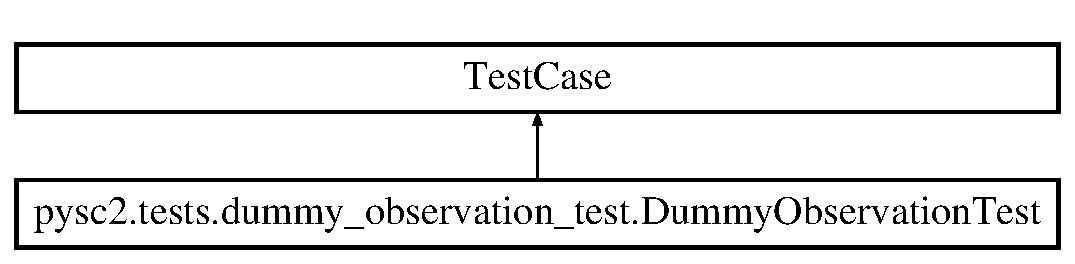
\includegraphics[height=2.000000cm]{classpysc2_1_1tests_1_1dummy__observation__test_1_1_dummy_observation_test}
\end{center}
\end{figure}
\subsection*{Public Member Functions}
\begin{DoxyCompactItemize}
\item 
def \mbox{\hyperlink{classpysc2_1_1tests_1_1dummy__observation__test_1_1_dummy_observation_test_a90c890d9d56733790183fe8dcc53a916}{set\+Up}} (self)
\item 
def \mbox{\hyperlink{classpysc2_1_1tests_1_1dummy__observation__test_1_1_dummy_observation_test_affe2dfa9a11280cca802b80ba8a869a0}{test\+Feature\+Screen\+Matches\+Spec}} (self)
\item 
def \mbox{\hyperlink{classpysc2_1_1tests_1_1dummy__observation__test_1_1_dummy_observation_test_a5c5ac3c3392eaad94fe6471e7cc9def0}{test\+Feature\+Minimap\+Matches\+Spec}} (self)
\item 
def \mbox{\hyperlink{classpysc2_1_1tests_1_1dummy__observation__test_1_1_dummy_observation_test_aad2ea391040824fc0fafce2e1977edec}{test\+Rgb\+Screen\+Matches\+Spec}} (self)
\item 
def \mbox{\hyperlink{classpysc2_1_1tests_1_1dummy__observation__test_1_1_dummy_observation_test_a1c3bb18eb8dafe864dff78378087640f}{test\+Rgb\+Minimap\+Matches\+Spec}} (self)
\item 
def \mbox{\hyperlink{classpysc2_1_1tests_1_1dummy__observation__test_1_1_dummy_observation_test_ace9d92fbc949b4d83b9bb2a1e30e296b}{test\+No\+Single\+Select}} (self)
\item 
def \mbox{\hyperlink{classpysc2_1_1tests_1_1dummy__observation__test_1_1_dummy_observation_test_a5c63e3a39253ff187c1287501a5e6aeb}{test\+With\+Single\+Select}} (self)
\item 
def \mbox{\hyperlink{classpysc2_1_1tests_1_1dummy__observation__test_1_1_dummy_observation_test_aa0a667046ce3bb0b9275d1a989a63034}{test\+No\+Multi\+Select}} (self)
\item 
def \mbox{\hyperlink{classpysc2_1_1tests_1_1dummy__observation__test_1_1_dummy_observation_test_af4726de0b495c433f04588fba6aa469d}{test\+With\+Multi\+Select}} (self)
\item 
def \mbox{\hyperlink{classpysc2_1_1tests_1_1dummy__observation__test_1_1_dummy_observation_test_a8109cde8b155117150fce42a1519f5d2}{test\+Feature\+Units\+Are\+Added}} (self)
\end{DoxyCompactItemize}


\subsection{Member Function Documentation}
\mbox{\Hypertarget{classpysc2_1_1tests_1_1dummy__observation__test_1_1_dummy_observation_test_a90c890d9d56733790183fe8dcc53a916}\label{classpysc2_1_1tests_1_1dummy__observation__test_1_1_dummy_observation_test_a90c890d9d56733790183fe8dcc53a916}} 
\index{pysc2\+::tests\+::dummy\+\_\+observation\+\_\+test\+::\+Dummy\+Observation\+Test@{pysc2\+::tests\+::dummy\+\_\+observation\+\_\+test\+::\+Dummy\+Observation\+Test}!set\+Up@{set\+Up}}
\index{set\+Up@{set\+Up}!pysc2\+::tests\+::dummy\+\_\+observation\+\_\+test\+::\+Dummy\+Observation\+Test@{pysc2\+::tests\+::dummy\+\_\+observation\+\_\+test\+::\+Dummy\+Observation\+Test}}
\subsubsection{\texorpdfstring{set\+Up()}{setUp()}}
{\footnotesize\ttfamily def pysc2.\+tests.\+dummy\+\_\+observation\+\_\+test.\+Dummy\+Observation\+Test.\+set\+Up (\begin{DoxyParamCaption}\item[{}]{self }\end{DoxyParamCaption})}

\mbox{\Hypertarget{classpysc2_1_1tests_1_1dummy__observation__test_1_1_dummy_observation_test_a5c5ac3c3392eaad94fe6471e7cc9def0}\label{classpysc2_1_1tests_1_1dummy__observation__test_1_1_dummy_observation_test_a5c5ac3c3392eaad94fe6471e7cc9def0}} 
\index{pysc2\+::tests\+::dummy\+\_\+observation\+\_\+test\+::\+Dummy\+Observation\+Test@{pysc2\+::tests\+::dummy\+\_\+observation\+\_\+test\+::\+Dummy\+Observation\+Test}!test\+Feature\+Minimap\+Matches\+Spec@{test\+Feature\+Minimap\+Matches\+Spec}}
\index{test\+Feature\+Minimap\+Matches\+Spec@{test\+Feature\+Minimap\+Matches\+Spec}!pysc2\+::tests\+::dummy\+\_\+observation\+\_\+test\+::\+Dummy\+Observation\+Test@{pysc2\+::tests\+::dummy\+\_\+observation\+\_\+test\+::\+Dummy\+Observation\+Test}}
\subsubsection{\texorpdfstring{test\+Feature\+Minimap\+Matches\+Spec()}{testFeatureMinimapMatchesSpec()}}
{\footnotesize\ttfamily def pysc2.\+tests.\+dummy\+\_\+observation\+\_\+test.\+Dummy\+Observation\+Test.\+test\+Feature\+Minimap\+Matches\+Spec (\begin{DoxyParamCaption}\item[{}]{self }\end{DoxyParamCaption})}

\mbox{\Hypertarget{classpysc2_1_1tests_1_1dummy__observation__test_1_1_dummy_observation_test_affe2dfa9a11280cca802b80ba8a869a0}\label{classpysc2_1_1tests_1_1dummy__observation__test_1_1_dummy_observation_test_affe2dfa9a11280cca802b80ba8a869a0}} 
\index{pysc2\+::tests\+::dummy\+\_\+observation\+\_\+test\+::\+Dummy\+Observation\+Test@{pysc2\+::tests\+::dummy\+\_\+observation\+\_\+test\+::\+Dummy\+Observation\+Test}!test\+Feature\+Screen\+Matches\+Spec@{test\+Feature\+Screen\+Matches\+Spec}}
\index{test\+Feature\+Screen\+Matches\+Spec@{test\+Feature\+Screen\+Matches\+Spec}!pysc2\+::tests\+::dummy\+\_\+observation\+\_\+test\+::\+Dummy\+Observation\+Test@{pysc2\+::tests\+::dummy\+\_\+observation\+\_\+test\+::\+Dummy\+Observation\+Test}}
\subsubsection{\texorpdfstring{test\+Feature\+Screen\+Matches\+Spec()}{testFeatureScreenMatchesSpec()}}
{\footnotesize\ttfamily def pysc2.\+tests.\+dummy\+\_\+observation\+\_\+test.\+Dummy\+Observation\+Test.\+test\+Feature\+Screen\+Matches\+Spec (\begin{DoxyParamCaption}\item[{}]{self }\end{DoxyParamCaption})}

\mbox{\Hypertarget{classpysc2_1_1tests_1_1dummy__observation__test_1_1_dummy_observation_test_a8109cde8b155117150fce42a1519f5d2}\label{classpysc2_1_1tests_1_1dummy__observation__test_1_1_dummy_observation_test_a8109cde8b155117150fce42a1519f5d2}} 
\index{pysc2\+::tests\+::dummy\+\_\+observation\+\_\+test\+::\+Dummy\+Observation\+Test@{pysc2\+::tests\+::dummy\+\_\+observation\+\_\+test\+::\+Dummy\+Observation\+Test}!test\+Feature\+Units\+Are\+Added@{test\+Feature\+Units\+Are\+Added}}
\index{test\+Feature\+Units\+Are\+Added@{test\+Feature\+Units\+Are\+Added}!pysc2\+::tests\+::dummy\+\_\+observation\+\_\+test\+::\+Dummy\+Observation\+Test@{pysc2\+::tests\+::dummy\+\_\+observation\+\_\+test\+::\+Dummy\+Observation\+Test}}
\subsubsection{\texorpdfstring{test\+Feature\+Units\+Are\+Added()}{testFeatureUnitsAreAdded()}}
{\footnotesize\ttfamily def pysc2.\+tests.\+dummy\+\_\+observation\+\_\+test.\+Dummy\+Observation\+Test.\+test\+Feature\+Units\+Are\+Added (\begin{DoxyParamCaption}\item[{}]{self }\end{DoxyParamCaption})}

\mbox{\Hypertarget{classpysc2_1_1tests_1_1dummy__observation__test_1_1_dummy_observation_test_aa0a667046ce3bb0b9275d1a989a63034}\label{classpysc2_1_1tests_1_1dummy__observation__test_1_1_dummy_observation_test_aa0a667046ce3bb0b9275d1a989a63034}} 
\index{pysc2\+::tests\+::dummy\+\_\+observation\+\_\+test\+::\+Dummy\+Observation\+Test@{pysc2\+::tests\+::dummy\+\_\+observation\+\_\+test\+::\+Dummy\+Observation\+Test}!test\+No\+Multi\+Select@{test\+No\+Multi\+Select}}
\index{test\+No\+Multi\+Select@{test\+No\+Multi\+Select}!pysc2\+::tests\+::dummy\+\_\+observation\+\_\+test\+::\+Dummy\+Observation\+Test@{pysc2\+::tests\+::dummy\+\_\+observation\+\_\+test\+::\+Dummy\+Observation\+Test}}
\subsubsection{\texorpdfstring{test\+No\+Multi\+Select()}{testNoMultiSelect()}}
{\footnotesize\ttfamily def pysc2.\+tests.\+dummy\+\_\+observation\+\_\+test.\+Dummy\+Observation\+Test.\+test\+No\+Multi\+Select (\begin{DoxyParamCaption}\item[{}]{self }\end{DoxyParamCaption})}

\mbox{\Hypertarget{classpysc2_1_1tests_1_1dummy__observation__test_1_1_dummy_observation_test_ace9d92fbc949b4d83b9bb2a1e30e296b}\label{classpysc2_1_1tests_1_1dummy__observation__test_1_1_dummy_observation_test_ace9d92fbc949b4d83b9bb2a1e30e296b}} 
\index{pysc2\+::tests\+::dummy\+\_\+observation\+\_\+test\+::\+Dummy\+Observation\+Test@{pysc2\+::tests\+::dummy\+\_\+observation\+\_\+test\+::\+Dummy\+Observation\+Test}!test\+No\+Single\+Select@{test\+No\+Single\+Select}}
\index{test\+No\+Single\+Select@{test\+No\+Single\+Select}!pysc2\+::tests\+::dummy\+\_\+observation\+\_\+test\+::\+Dummy\+Observation\+Test@{pysc2\+::tests\+::dummy\+\_\+observation\+\_\+test\+::\+Dummy\+Observation\+Test}}
\subsubsection{\texorpdfstring{test\+No\+Single\+Select()}{testNoSingleSelect()}}
{\footnotesize\ttfamily def pysc2.\+tests.\+dummy\+\_\+observation\+\_\+test.\+Dummy\+Observation\+Test.\+test\+No\+Single\+Select (\begin{DoxyParamCaption}\item[{}]{self }\end{DoxyParamCaption})}

\mbox{\Hypertarget{classpysc2_1_1tests_1_1dummy__observation__test_1_1_dummy_observation_test_a1c3bb18eb8dafe864dff78378087640f}\label{classpysc2_1_1tests_1_1dummy__observation__test_1_1_dummy_observation_test_a1c3bb18eb8dafe864dff78378087640f}} 
\index{pysc2\+::tests\+::dummy\+\_\+observation\+\_\+test\+::\+Dummy\+Observation\+Test@{pysc2\+::tests\+::dummy\+\_\+observation\+\_\+test\+::\+Dummy\+Observation\+Test}!test\+Rgb\+Minimap\+Matches\+Spec@{test\+Rgb\+Minimap\+Matches\+Spec}}
\index{test\+Rgb\+Minimap\+Matches\+Spec@{test\+Rgb\+Minimap\+Matches\+Spec}!pysc2\+::tests\+::dummy\+\_\+observation\+\_\+test\+::\+Dummy\+Observation\+Test@{pysc2\+::tests\+::dummy\+\_\+observation\+\_\+test\+::\+Dummy\+Observation\+Test}}
\subsubsection{\texorpdfstring{test\+Rgb\+Minimap\+Matches\+Spec()}{testRgbMinimapMatchesSpec()}}
{\footnotesize\ttfamily def pysc2.\+tests.\+dummy\+\_\+observation\+\_\+test.\+Dummy\+Observation\+Test.\+test\+Rgb\+Minimap\+Matches\+Spec (\begin{DoxyParamCaption}\item[{}]{self }\end{DoxyParamCaption})}

\mbox{\Hypertarget{classpysc2_1_1tests_1_1dummy__observation__test_1_1_dummy_observation_test_aad2ea391040824fc0fafce2e1977edec}\label{classpysc2_1_1tests_1_1dummy__observation__test_1_1_dummy_observation_test_aad2ea391040824fc0fafce2e1977edec}} 
\index{pysc2\+::tests\+::dummy\+\_\+observation\+\_\+test\+::\+Dummy\+Observation\+Test@{pysc2\+::tests\+::dummy\+\_\+observation\+\_\+test\+::\+Dummy\+Observation\+Test}!test\+Rgb\+Screen\+Matches\+Spec@{test\+Rgb\+Screen\+Matches\+Spec}}
\index{test\+Rgb\+Screen\+Matches\+Spec@{test\+Rgb\+Screen\+Matches\+Spec}!pysc2\+::tests\+::dummy\+\_\+observation\+\_\+test\+::\+Dummy\+Observation\+Test@{pysc2\+::tests\+::dummy\+\_\+observation\+\_\+test\+::\+Dummy\+Observation\+Test}}
\subsubsection{\texorpdfstring{test\+Rgb\+Screen\+Matches\+Spec()}{testRgbScreenMatchesSpec()}}
{\footnotesize\ttfamily def pysc2.\+tests.\+dummy\+\_\+observation\+\_\+test.\+Dummy\+Observation\+Test.\+test\+Rgb\+Screen\+Matches\+Spec (\begin{DoxyParamCaption}\item[{}]{self }\end{DoxyParamCaption})}

\mbox{\Hypertarget{classpysc2_1_1tests_1_1dummy__observation__test_1_1_dummy_observation_test_af4726de0b495c433f04588fba6aa469d}\label{classpysc2_1_1tests_1_1dummy__observation__test_1_1_dummy_observation_test_af4726de0b495c433f04588fba6aa469d}} 
\index{pysc2\+::tests\+::dummy\+\_\+observation\+\_\+test\+::\+Dummy\+Observation\+Test@{pysc2\+::tests\+::dummy\+\_\+observation\+\_\+test\+::\+Dummy\+Observation\+Test}!test\+With\+Multi\+Select@{test\+With\+Multi\+Select}}
\index{test\+With\+Multi\+Select@{test\+With\+Multi\+Select}!pysc2\+::tests\+::dummy\+\_\+observation\+\_\+test\+::\+Dummy\+Observation\+Test@{pysc2\+::tests\+::dummy\+\_\+observation\+\_\+test\+::\+Dummy\+Observation\+Test}}
\subsubsection{\texorpdfstring{test\+With\+Multi\+Select()}{testWithMultiSelect()}}
{\footnotesize\ttfamily def pysc2.\+tests.\+dummy\+\_\+observation\+\_\+test.\+Dummy\+Observation\+Test.\+test\+With\+Multi\+Select (\begin{DoxyParamCaption}\item[{}]{self }\end{DoxyParamCaption})}

\mbox{\Hypertarget{classpysc2_1_1tests_1_1dummy__observation__test_1_1_dummy_observation_test_a5c63e3a39253ff187c1287501a5e6aeb}\label{classpysc2_1_1tests_1_1dummy__observation__test_1_1_dummy_observation_test_a5c63e3a39253ff187c1287501a5e6aeb}} 
\index{pysc2\+::tests\+::dummy\+\_\+observation\+\_\+test\+::\+Dummy\+Observation\+Test@{pysc2\+::tests\+::dummy\+\_\+observation\+\_\+test\+::\+Dummy\+Observation\+Test}!test\+With\+Single\+Select@{test\+With\+Single\+Select}}
\index{test\+With\+Single\+Select@{test\+With\+Single\+Select}!pysc2\+::tests\+::dummy\+\_\+observation\+\_\+test\+::\+Dummy\+Observation\+Test@{pysc2\+::tests\+::dummy\+\_\+observation\+\_\+test\+::\+Dummy\+Observation\+Test}}
\subsubsection{\texorpdfstring{test\+With\+Single\+Select()}{testWithSingleSelect()}}
{\footnotesize\ttfamily def pysc2.\+tests.\+dummy\+\_\+observation\+\_\+test.\+Dummy\+Observation\+Test.\+test\+With\+Single\+Select (\begin{DoxyParamCaption}\item[{}]{self }\end{DoxyParamCaption})}



The documentation for this class was generated from the following file\+:\begin{DoxyCompactItemize}
\item 
tests/\mbox{\hyperlink{dummy__observation__test_8py}{dummy\+\_\+observation\+\_\+test.\+py}}\end{DoxyCompactItemize}

\hypertarget{classpysc2_1_1maps_1_1lib_1_1_duplicate_map_exception}{}\section{pysc2.\+maps.\+lib.\+Duplicate\+Map\+Exception Class Reference}
\label{classpysc2_1_1maps_1_1lib_1_1_duplicate_map_exception}\index{pysc2.\+maps.\+lib.\+Duplicate\+Map\+Exception@{pysc2.\+maps.\+lib.\+Duplicate\+Map\+Exception}}
Inheritance diagram for pysc2.\+maps.\+lib.\+Duplicate\+Map\+Exception\+:\begin{figure}[H]
\begin{center}
\leavevmode
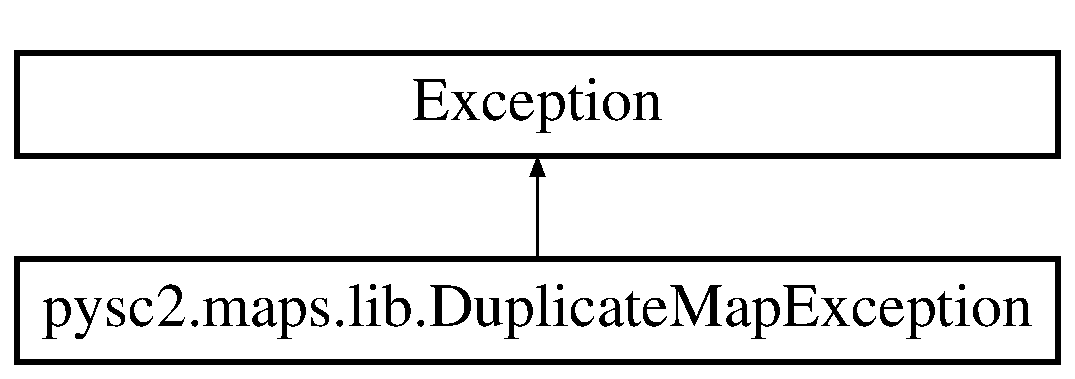
\includegraphics[height=2.000000cm]{classpysc2_1_1maps_1_1lib_1_1_duplicate_map_exception}
\end{center}
\end{figure}


The documentation for this class was generated from the following file\+:\begin{DoxyCompactItemize}
\item 
maps/\mbox{\hyperlink{maps_2lib_8py}{lib.\+py}}\end{DoxyCompactItemize}

\hypertarget{classpysc2_1_1lib_1_1features_1_1_effects}{}\section{pysc2.\+lib.\+features.\+Effects Class Reference}
\label{classpysc2_1_1lib_1_1features_1_1_effects}\index{pysc2.\+lib.\+features.\+Effects@{pysc2.\+lib.\+features.\+Effects}}
Inheritance diagram for pysc2.\+lib.\+features.\+Effects\+:\begin{figure}[H]
\begin{center}
\leavevmode
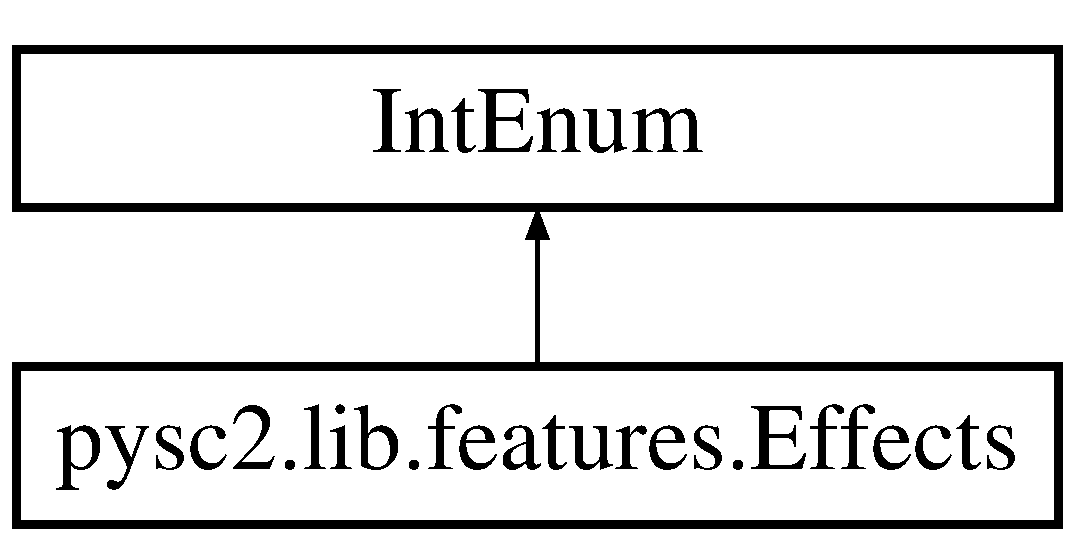
\includegraphics[height=2.000000cm]{classpysc2_1_1lib_1_1features_1_1_effects}
\end{center}
\end{figure}
\subsection*{Static Public Attributes}
\begin{DoxyCompactItemize}
\item 
int \mbox{\hyperlink{classpysc2_1_1lib_1_1features_1_1_effects_a13a840bd029e23e205a91edfafbaa8c3}{Psi\+Storm}} = 1
\item 
int \mbox{\hyperlink{classpysc2_1_1lib_1_1features_1_1_effects_ab74615673cebae9903287968e0b949f0}{Guardian\+Shield}} = 2
\item 
int \mbox{\hyperlink{classpysc2_1_1lib_1_1features_1_1_effects_a48a90cc392c74c0c17c91229a0d8d1c4}{Temporal\+Field\+Growing}} = 3
\item 
int \mbox{\hyperlink{classpysc2_1_1lib_1_1features_1_1_effects_aed31efb4698e8fd3c26a6cfe183c590f}{Temporal\+Field}} = 4
\item 
int \mbox{\hyperlink{classpysc2_1_1lib_1_1features_1_1_effects_a19f880ae3f13c285675db46675e86db6}{Thermal\+Lance}} = 5
\item 
int \mbox{\hyperlink{classpysc2_1_1lib_1_1features_1_1_effects_a537c89bacceab397addc4d7cabf56042}{Scanner\+Sweep}} = 6
\item 
int \mbox{\hyperlink{classpysc2_1_1lib_1_1features_1_1_effects_ae61b599ec15cf0cac0dfa54e7e5ffb40}{Nuke\+Dot}} = 7
\item 
int \mbox{\hyperlink{classpysc2_1_1lib_1_1features_1_1_effects_af0e07c05976e507275f651a7e1ca6017}{Liberator\+Defender\+Zone\+Setup}} = 8
\item 
int \mbox{\hyperlink{classpysc2_1_1lib_1_1features_1_1_effects_af0c1ed1fdfea242888e216419ca05c10}{Liberator\+Defender\+Zone}} = 9
\item 
int \mbox{\hyperlink{classpysc2_1_1lib_1_1features_1_1_effects_aef0d51c221a9c1b80d6e7f3c11986b9d}{Blinding\+Cloud}} = 10
\item 
int \mbox{\hyperlink{classpysc2_1_1lib_1_1features_1_1_effects_acfd91c4b7c29f824809dbc39f0a71e04}{Corrosive\+Bile}} = 11
\item 
int \mbox{\hyperlink{classpysc2_1_1lib_1_1features_1_1_effects_a9be68980993549c17e5cb108a1c75af8}{Lurker\+Spines}} = 12
\end{DoxyCompactItemize}


\subsection{Detailed Description}
\begin{DoxyVerb}Values for the `effects` feature layer.\end{DoxyVerb}
 

\subsection{Member Data Documentation}
\mbox{\Hypertarget{classpysc2_1_1lib_1_1features_1_1_effects_aef0d51c221a9c1b80d6e7f3c11986b9d}\label{classpysc2_1_1lib_1_1features_1_1_effects_aef0d51c221a9c1b80d6e7f3c11986b9d}} 
\index{pysc2\+::lib\+::features\+::\+Effects@{pysc2\+::lib\+::features\+::\+Effects}!Blinding\+Cloud@{Blinding\+Cloud}}
\index{Blinding\+Cloud@{Blinding\+Cloud}!pysc2\+::lib\+::features\+::\+Effects@{pysc2\+::lib\+::features\+::\+Effects}}
\subsubsection{\texorpdfstring{Blinding\+Cloud}{BlindingCloud}}
{\footnotesize\ttfamily int pysc2.\+lib.\+features.\+Effects.\+Blinding\+Cloud = 10\hspace{0.3cm}{\ttfamily [static]}}

\mbox{\Hypertarget{classpysc2_1_1lib_1_1features_1_1_effects_acfd91c4b7c29f824809dbc39f0a71e04}\label{classpysc2_1_1lib_1_1features_1_1_effects_acfd91c4b7c29f824809dbc39f0a71e04}} 
\index{pysc2\+::lib\+::features\+::\+Effects@{pysc2\+::lib\+::features\+::\+Effects}!Corrosive\+Bile@{Corrosive\+Bile}}
\index{Corrosive\+Bile@{Corrosive\+Bile}!pysc2\+::lib\+::features\+::\+Effects@{pysc2\+::lib\+::features\+::\+Effects}}
\subsubsection{\texorpdfstring{Corrosive\+Bile}{CorrosiveBile}}
{\footnotesize\ttfamily int pysc2.\+lib.\+features.\+Effects.\+Corrosive\+Bile = 11\hspace{0.3cm}{\ttfamily [static]}}

\mbox{\Hypertarget{classpysc2_1_1lib_1_1features_1_1_effects_ab74615673cebae9903287968e0b949f0}\label{classpysc2_1_1lib_1_1features_1_1_effects_ab74615673cebae9903287968e0b949f0}} 
\index{pysc2\+::lib\+::features\+::\+Effects@{pysc2\+::lib\+::features\+::\+Effects}!Guardian\+Shield@{Guardian\+Shield}}
\index{Guardian\+Shield@{Guardian\+Shield}!pysc2\+::lib\+::features\+::\+Effects@{pysc2\+::lib\+::features\+::\+Effects}}
\subsubsection{\texorpdfstring{Guardian\+Shield}{GuardianShield}}
{\footnotesize\ttfamily int pysc2.\+lib.\+features.\+Effects.\+Guardian\+Shield = 2\hspace{0.3cm}{\ttfamily [static]}}

\mbox{\Hypertarget{classpysc2_1_1lib_1_1features_1_1_effects_af0c1ed1fdfea242888e216419ca05c10}\label{classpysc2_1_1lib_1_1features_1_1_effects_af0c1ed1fdfea242888e216419ca05c10}} 
\index{pysc2\+::lib\+::features\+::\+Effects@{pysc2\+::lib\+::features\+::\+Effects}!Liberator\+Defender\+Zone@{Liberator\+Defender\+Zone}}
\index{Liberator\+Defender\+Zone@{Liberator\+Defender\+Zone}!pysc2\+::lib\+::features\+::\+Effects@{pysc2\+::lib\+::features\+::\+Effects}}
\subsubsection{\texorpdfstring{Liberator\+Defender\+Zone}{LiberatorDefenderZone}}
{\footnotesize\ttfamily int pysc2.\+lib.\+features.\+Effects.\+Liberator\+Defender\+Zone = 9\hspace{0.3cm}{\ttfamily [static]}}

\mbox{\Hypertarget{classpysc2_1_1lib_1_1features_1_1_effects_af0e07c05976e507275f651a7e1ca6017}\label{classpysc2_1_1lib_1_1features_1_1_effects_af0e07c05976e507275f651a7e1ca6017}} 
\index{pysc2\+::lib\+::features\+::\+Effects@{pysc2\+::lib\+::features\+::\+Effects}!Liberator\+Defender\+Zone\+Setup@{Liberator\+Defender\+Zone\+Setup}}
\index{Liberator\+Defender\+Zone\+Setup@{Liberator\+Defender\+Zone\+Setup}!pysc2\+::lib\+::features\+::\+Effects@{pysc2\+::lib\+::features\+::\+Effects}}
\subsubsection{\texorpdfstring{Liberator\+Defender\+Zone\+Setup}{LiberatorDefenderZoneSetup}}
{\footnotesize\ttfamily int pysc2.\+lib.\+features.\+Effects.\+Liberator\+Defender\+Zone\+Setup = 8\hspace{0.3cm}{\ttfamily [static]}}

\mbox{\Hypertarget{classpysc2_1_1lib_1_1features_1_1_effects_a9be68980993549c17e5cb108a1c75af8}\label{classpysc2_1_1lib_1_1features_1_1_effects_a9be68980993549c17e5cb108a1c75af8}} 
\index{pysc2\+::lib\+::features\+::\+Effects@{pysc2\+::lib\+::features\+::\+Effects}!Lurker\+Spines@{Lurker\+Spines}}
\index{Lurker\+Spines@{Lurker\+Spines}!pysc2\+::lib\+::features\+::\+Effects@{pysc2\+::lib\+::features\+::\+Effects}}
\subsubsection{\texorpdfstring{Lurker\+Spines}{LurkerSpines}}
{\footnotesize\ttfamily int pysc2.\+lib.\+features.\+Effects.\+Lurker\+Spines = 12\hspace{0.3cm}{\ttfamily [static]}}

\mbox{\Hypertarget{classpysc2_1_1lib_1_1features_1_1_effects_ae61b599ec15cf0cac0dfa54e7e5ffb40}\label{classpysc2_1_1lib_1_1features_1_1_effects_ae61b599ec15cf0cac0dfa54e7e5ffb40}} 
\index{pysc2\+::lib\+::features\+::\+Effects@{pysc2\+::lib\+::features\+::\+Effects}!Nuke\+Dot@{Nuke\+Dot}}
\index{Nuke\+Dot@{Nuke\+Dot}!pysc2\+::lib\+::features\+::\+Effects@{pysc2\+::lib\+::features\+::\+Effects}}
\subsubsection{\texorpdfstring{Nuke\+Dot}{NukeDot}}
{\footnotesize\ttfamily int pysc2.\+lib.\+features.\+Effects.\+Nuke\+Dot = 7\hspace{0.3cm}{\ttfamily [static]}}

\mbox{\Hypertarget{classpysc2_1_1lib_1_1features_1_1_effects_a13a840bd029e23e205a91edfafbaa8c3}\label{classpysc2_1_1lib_1_1features_1_1_effects_a13a840bd029e23e205a91edfafbaa8c3}} 
\index{pysc2\+::lib\+::features\+::\+Effects@{pysc2\+::lib\+::features\+::\+Effects}!Psi\+Storm@{Psi\+Storm}}
\index{Psi\+Storm@{Psi\+Storm}!pysc2\+::lib\+::features\+::\+Effects@{pysc2\+::lib\+::features\+::\+Effects}}
\subsubsection{\texorpdfstring{Psi\+Storm}{PsiStorm}}
{\footnotesize\ttfamily int pysc2.\+lib.\+features.\+Effects.\+Psi\+Storm = 1\hspace{0.3cm}{\ttfamily [static]}}

\mbox{\Hypertarget{classpysc2_1_1lib_1_1features_1_1_effects_a537c89bacceab397addc4d7cabf56042}\label{classpysc2_1_1lib_1_1features_1_1_effects_a537c89bacceab397addc4d7cabf56042}} 
\index{pysc2\+::lib\+::features\+::\+Effects@{pysc2\+::lib\+::features\+::\+Effects}!Scanner\+Sweep@{Scanner\+Sweep}}
\index{Scanner\+Sweep@{Scanner\+Sweep}!pysc2\+::lib\+::features\+::\+Effects@{pysc2\+::lib\+::features\+::\+Effects}}
\subsubsection{\texorpdfstring{Scanner\+Sweep}{ScannerSweep}}
{\footnotesize\ttfamily int pysc2.\+lib.\+features.\+Effects.\+Scanner\+Sweep = 6\hspace{0.3cm}{\ttfamily [static]}}

\mbox{\Hypertarget{classpysc2_1_1lib_1_1features_1_1_effects_aed31efb4698e8fd3c26a6cfe183c590f}\label{classpysc2_1_1lib_1_1features_1_1_effects_aed31efb4698e8fd3c26a6cfe183c590f}} 
\index{pysc2\+::lib\+::features\+::\+Effects@{pysc2\+::lib\+::features\+::\+Effects}!Temporal\+Field@{Temporal\+Field}}
\index{Temporal\+Field@{Temporal\+Field}!pysc2\+::lib\+::features\+::\+Effects@{pysc2\+::lib\+::features\+::\+Effects}}
\subsubsection{\texorpdfstring{Temporal\+Field}{TemporalField}}
{\footnotesize\ttfamily int pysc2.\+lib.\+features.\+Effects.\+Temporal\+Field = 4\hspace{0.3cm}{\ttfamily [static]}}

\mbox{\Hypertarget{classpysc2_1_1lib_1_1features_1_1_effects_a48a90cc392c74c0c17c91229a0d8d1c4}\label{classpysc2_1_1lib_1_1features_1_1_effects_a48a90cc392c74c0c17c91229a0d8d1c4}} 
\index{pysc2\+::lib\+::features\+::\+Effects@{pysc2\+::lib\+::features\+::\+Effects}!Temporal\+Field\+Growing@{Temporal\+Field\+Growing}}
\index{Temporal\+Field\+Growing@{Temporal\+Field\+Growing}!pysc2\+::lib\+::features\+::\+Effects@{pysc2\+::lib\+::features\+::\+Effects}}
\subsubsection{\texorpdfstring{Temporal\+Field\+Growing}{TemporalFieldGrowing}}
{\footnotesize\ttfamily int pysc2.\+lib.\+features.\+Effects.\+Temporal\+Field\+Growing = 3\hspace{0.3cm}{\ttfamily [static]}}

\mbox{\Hypertarget{classpysc2_1_1lib_1_1features_1_1_effects_a19f880ae3f13c285675db46675e86db6}\label{classpysc2_1_1lib_1_1features_1_1_effects_a19f880ae3f13c285675db46675e86db6}} 
\index{pysc2\+::lib\+::features\+::\+Effects@{pysc2\+::lib\+::features\+::\+Effects}!Thermal\+Lance@{Thermal\+Lance}}
\index{Thermal\+Lance@{Thermal\+Lance}!pysc2\+::lib\+::features\+::\+Effects@{pysc2\+::lib\+::features\+::\+Effects}}
\subsubsection{\texorpdfstring{Thermal\+Lance}{ThermalLance}}
{\footnotesize\ttfamily int pysc2.\+lib.\+features.\+Effects.\+Thermal\+Lance = 5\hspace{0.3cm}{\ttfamily [static]}}



The documentation for this class was generated from the following file\+:\begin{DoxyCompactItemize}
\item 
lib/\mbox{\hyperlink{features_8py}{features.\+py}}\end{DoxyCompactItemize}

\hypertarget{classpysc2_1_1lib_1_1point__test_1_1_fake_point}{}\section{pysc2.\+lib.\+point\+\_\+test.\+Fake\+Point Class Reference}
\label{classpysc2_1_1lib_1_1point__test_1_1_fake_point}\index{pysc2.\+lib.\+point\+\_\+test.\+Fake\+Point@{pysc2.\+lib.\+point\+\_\+test.\+Fake\+Point}}
Inheritance diagram for pysc2.\+lib.\+point\+\_\+test.\+Fake\+Point\+:\begin{figure}[H]
\begin{center}
\leavevmode
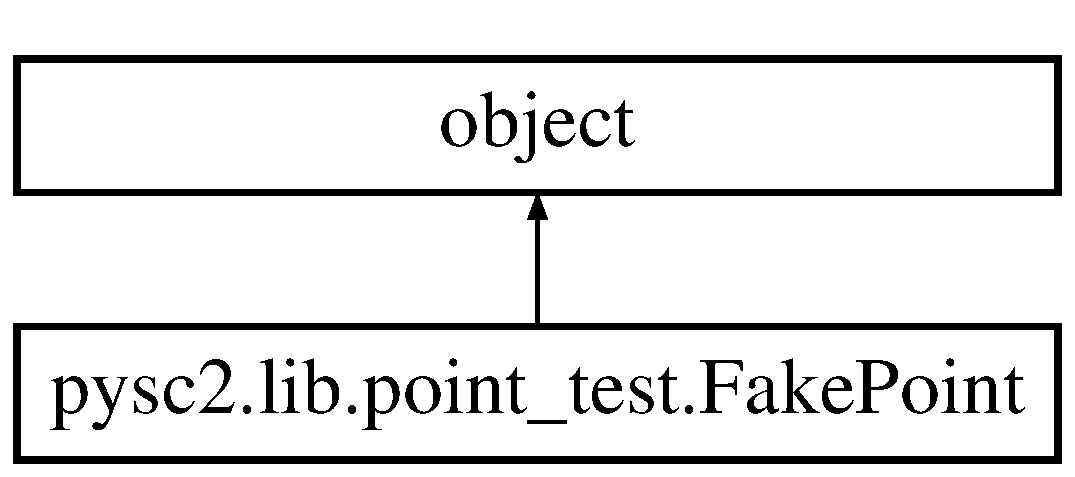
\includegraphics[height=2.000000cm]{classpysc2_1_1lib_1_1point__test_1_1_fake_point}
\end{center}
\end{figure}
\subsection*{Public Member Functions}
\begin{DoxyCompactItemize}
\item 
def \mbox{\hyperlink{classpysc2_1_1lib_1_1point__test_1_1_fake_point_a477a3ccac64bf883f4302776c25e64fd}{\+\_\+\+\_\+init\+\_\+\+\_\+}} (self)
\end{DoxyCompactItemize}
\subsection*{Public Attributes}
\begin{DoxyCompactItemize}
\item 
\mbox{\hyperlink{classpysc2_1_1lib_1_1point__test_1_1_fake_point_af44ff09f18ad5a5f4788e5d0cc8e28aa}{x}}
\item 
\mbox{\hyperlink{classpysc2_1_1lib_1_1point__test_1_1_fake_point_abdf10860fd63baac01c2c3e12833876b}{y}}
\end{DoxyCompactItemize}


\subsection{Constructor \& Destructor Documentation}
\mbox{\Hypertarget{classpysc2_1_1lib_1_1point__test_1_1_fake_point_a477a3ccac64bf883f4302776c25e64fd}\label{classpysc2_1_1lib_1_1point__test_1_1_fake_point_a477a3ccac64bf883f4302776c25e64fd}} 
\index{pysc2\+::lib\+::point\+\_\+test\+::\+Fake\+Point@{pysc2\+::lib\+::point\+\_\+test\+::\+Fake\+Point}!\+\_\+\+\_\+init\+\_\+\+\_\+@{\+\_\+\+\_\+init\+\_\+\+\_\+}}
\index{\+\_\+\+\_\+init\+\_\+\+\_\+@{\+\_\+\+\_\+init\+\_\+\+\_\+}!pysc2\+::lib\+::point\+\_\+test\+::\+Fake\+Point@{pysc2\+::lib\+::point\+\_\+test\+::\+Fake\+Point}}
\subsubsection{\texorpdfstring{\+\_\+\+\_\+init\+\_\+\+\_\+()}{\_\_init\_\_()}}
{\footnotesize\ttfamily def pysc2.\+lib.\+point\+\_\+test.\+Fake\+Point.\+\_\+\+\_\+init\+\_\+\+\_\+ (\begin{DoxyParamCaption}\item[{}]{self }\end{DoxyParamCaption})}



\subsection{Member Data Documentation}
\mbox{\Hypertarget{classpysc2_1_1lib_1_1point__test_1_1_fake_point_af44ff09f18ad5a5f4788e5d0cc8e28aa}\label{classpysc2_1_1lib_1_1point__test_1_1_fake_point_af44ff09f18ad5a5f4788e5d0cc8e28aa}} 
\index{pysc2\+::lib\+::point\+\_\+test\+::\+Fake\+Point@{pysc2\+::lib\+::point\+\_\+test\+::\+Fake\+Point}!x@{x}}
\index{x@{x}!pysc2\+::lib\+::point\+\_\+test\+::\+Fake\+Point@{pysc2\+::lib\+::point\+\_\+test\+::\+Fake\+Point}}
\subsubsection{\texorpdfstring{x}{x}}
{\footnotesize\ttfamily pysc2.\+lib.\+point\+\_\+test.\+Fake\+Point.\+x}

\mbox{\Hypertarget{classpysc2_1_1lib_1_1point__test_1_1_fake_point_abdf10860fd63baac01c2c3e12833876b}\label{classpysc2_1_1lib_1_1point__test_1_1_fake_point_abdf10860fd63baac01c2c3e12833876b}} 
\index{pysc2\+::lib\+::point\+\_\+test\+::\+Fake\+Point@{pysc2\+::lib\+::point\+\_\+test\+::\+Fake\+Point}!y@{y}}
\index{y@{y}!pysc2\+::lib\+::point\+\_\+test\+::\+Fake\+Point@{pysc2\+::lib\+::point\+\_\+test\+::\+Fake\+Point}}
\subsubsection{\texorpdfstring{y}{y}}
{\footnotesize\ttfamily pysc2.\+lib.\+point\+\_\+test.\+Fake\+Point.\+y}



The documentation for this class was generated from the following file\+:\begin{DoxyCompactItemize}
\item 
lib/\mbox{\hyperlink{point__test_8py}{point\+\_\+test.\+py}}\end{DoxyCompactItemize}

\hypertarget{classpysc2_1_1lib_1_1stopwatch_1_1_fake_stop_watch_context}{}\section{pysc2.\+lib.\+stopwatch.\+Fake\+Stop\+Watch\+Context Class Reference}
\label{classpysc2_1_1lib_1_1stopwatch_1_1_fake_stop_watch_context}\index{pysc2.\+lib.\+stopwatch.\+Fake\+Stop\+Watch\+Context@{pysc2.\+lib.\+stopwatch.\+Fake\+Stop\+Watch\+Context}}
Inheritance diagram for pysc2.\+lib.\+stopwatch.\+Fake\+Stop\+Watch\+Context\+:\begin{figure}[H]
\begin{center}
\leavevmode
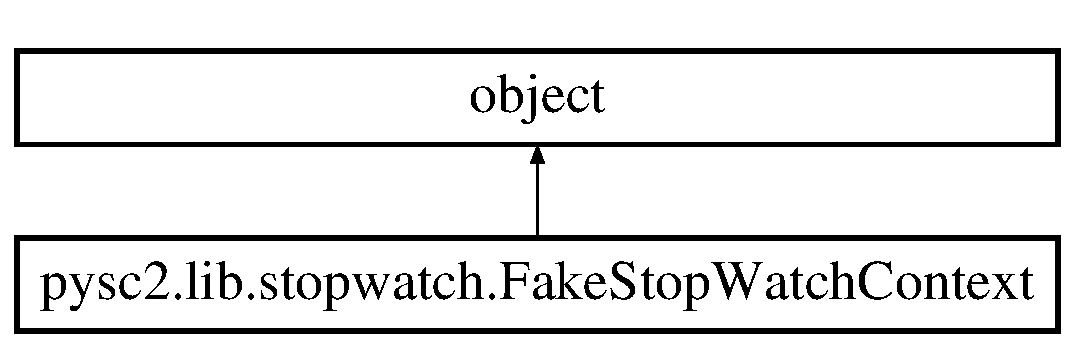
\includegraphics[height=2.000000cm]{classpysc2_1_1lib_1_1stopwatch_1_1_fake_stop_watch_context}
\end{center}
\end{figure}
\subsection*{Public Member Functions}
\begin{DoxyCompactItemize}
\item 
def \mbox{\hyperlink{classpysc2_1_1lib_1_1stopwatch_1_1_fake_stop_watch_context_a6f9d0d3e72aecb0fa76716d5a4ecc71d}{\+\_\+\+\_\+enter\+\_\+\+\_\+}} (self)
\item 
def \mbox{\hyperlink{classpysc2_1_1lib_1_1stopwatch_1_1_fake_stop_watch_context_a039be4e6cc198a84e03e20002d97d34f}{\+\_\+\+\_\+exit\+\_\+\+\_\+}} (self, unused\+\_\+exception\+\_\+type, unused\+\_\+exc\+\_\+value, unused\+\_\+traceback)
\end{DoxyCompactItemize}


\subsection{Detailed Description}
\begin{DoxyVerb}A fake stopwatch context for when the stopwatch is too slow or unneeded.\end{DoxyVerb}
 

\subsection{Member Function Documentation}
\mbox{\Hypertarget{classpysc2_1_1lib_1_1stopwatch_1_1_fake_stop_watch_context_a6f9d0d3e72aecb0fa76716d5a4ecc71d}\label{classpysc2_1_1lib_1_1stopwatch_1_1_fake_stop_watch_context_a6f9d0d3e72aecb0fa76716d5a4ecc71d}} 
\index{pysc2\+::lib\+::stopwatch\+::\+Fake\+Stop\+Watch\+Context@{pysc2\+::lib\+::stopwatch\+::\+Fake\+Stop\+Watch\+Context}!\+\_\+\+\_\+enter\+\_\+\+\_\+@{\+\_\+\+\_\+enter\+\_\+\+\_\+}}
\index{\+\_\+\+\_\+enter\+\_\+\+\_\+@{\+\_\+\+\_\+enter\+\_\+\+\_\+}!pysc2\+::lib\+::stopwatch\+::\+Fake\+Stop\+Watch\+Context@{pysc2\+::lib\+::stopwatch\+::\+Fake\+Stop\+Watch\+Context}}
\subsubsection{\texorpdfstring{\+\_\+\+\_\+enter\+\_\+\+\_\+()}{\_\_enter\_\_()}}
{\footnotesize\ttfamily def pysc2.\+lib.\+stopwatch.\+Fake\+Stop\+Watch\+Context.\+\_\+\+\_\+enter\+\_\+\+\_\+ (\begin{DoxyParamCaption}\item[{}]{self }\end{DoxyParamCaption})}

\mbox{\Hypertarget{classpysc2_1_1lib_1_1stopwatch_1_1_fake_stop_watch_context_a039be4e6cc198a84e03e20002d97d34f}\label{classpysc2_1_1lib_1_1stopwatch_1_1_fake_stop_watch_context_a039be4e6cc198a84e03e20002d97d34f}} 
\index{pysc2\+::lib\+::stopwatch\+::\+Fake\+Stop\+Watch\+Context@{pysc2\+::lib\+::stopwatch\+::\+Fake\+Stop\+Watch\+Context}!\+\_\+\+\_\+exit\+\_\+\+\_\+@{\+\_\+\+\_\+exit\+\_\+\+\_\+}}
\index{\+\_\+\+\_\+exit\+\_\+\+\_\+@{\+\_\+\+\_\+exit\+\_\+\+\_\+}!pysc2\+::lib\+::stopwatch\+::\+Fake\+Stop\+Watch\+Context@{pysc2\+::lib\+::stopwatch\+::\+Fake\+Stop\+Watch\+Context}}
\subsubsection{\texorpdfstring{\+\_\+\+\_\+exit\+\_\+\+\_\+()}{\_\_exit\_\_()}}
{\footnotesize\ttfamily def pysc2.\+lib.\+stopwatch.\+Fake\+Stop\+Watch\+Context.\+\_\+\+\_\+exit\+\_\+\+\_\+ (\begin{DoxyParamCaption}\item[{}]{self,  }\item[{}]{unused\+\_\+exception\+\_\+type,  }\item[{}]{unused\+\_\+exc\+\_\+value,  }\item[{}]{unused\+\_\+traceback }\end{DoxyParamCaption})}



The documentation for this class was generated from the following file\+:\begin{DoxyCompactItemize}
\item 
lib/\mbox{\hyperlink{stopwatch_8py}{stopwatch.\+py}}\end{DoxyCompactItemize}

\hypertarget{classpysc2_1_1lib_1_1features_1_1_feature}{}\section{pysc2.\+lib.\+features.\+Feature Class Reference}
\label{classpysc2_1_1lib_1_1features_1_1_feature}\index{pysc2.\+lib.\+features.\+Feature@{pysc2.\+lib.\+features.\+Feature}}
Inheritance diagram for pysc2.\+lib.\+features.\+Feature\+:\begin{figure}[H]
\begin{center}
\leavevmode
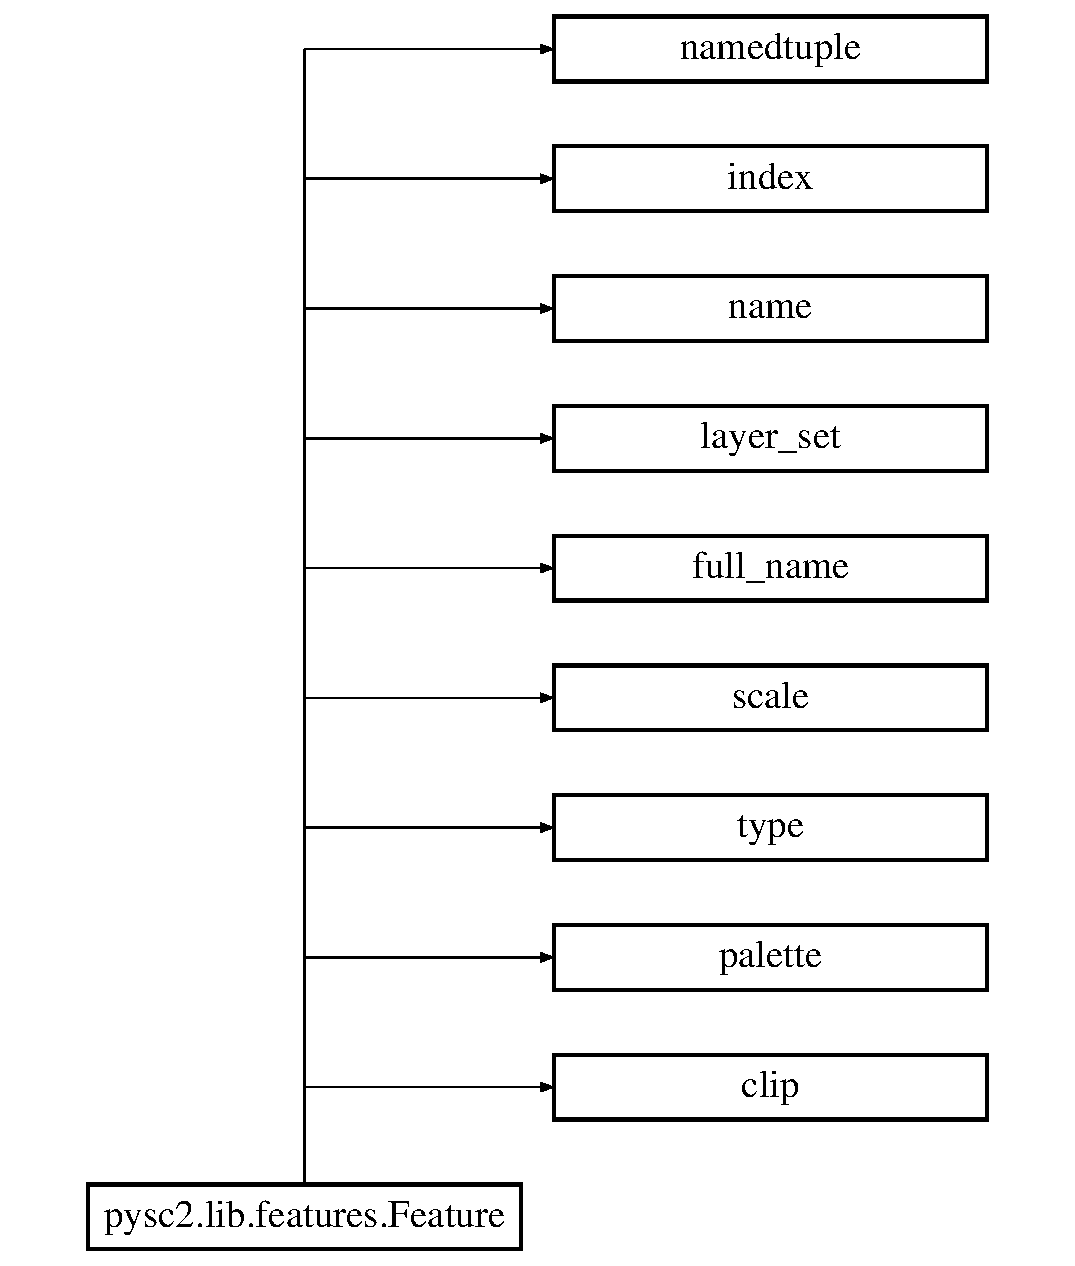
\includegraphics[height=10.000000cm]{classpysc2_1_1lib_1_1features_1_1_feature}
\end{center}
\end{figure}
\subsection*{Public Member Functions}
\begin{DoxyCompactItemize}
\item 
def \mbox{\hyperlink{classpysc2_1_1lib_1_1features_1_1_feature_a840859c8cc0f2bc3c80b665a38e879d7}{unpack}} (self, obs)
\item 
def \mbox{\hyperlink{classpysc2_1_1lib_1_1features_1_1_feature_a08f6ecbdfc49803c7221b5948d91df9e}{color}} (self, plane)
\end{DoxyCompactItemize}
\subsection*{Static Public Member Functions}
\begin{DoxyCompactItemize}
\item 
def \mbox{\hyperlink{classpysc2_1_1lib_1_1features_1_1_feature_ae2deeb3c743654425193f0b225c388e8}{unpack\+\_\+layer}} (plane)
\item 
def \mbox{\hyperlink{classpysc2_1_1lib_1_1features_1_1_feature_addc5dd18d59ef32762876df736f4509d}{unpack\+\_\+rgb\+\_\+image}} (plane)
\end{DoxyCompactItemize}
\subsection*{Static Public Attributes}
\begin{DoxyCompactItemize}
\item 
dictionary \mbox{\hyperlink{classpysc2_1_1lib_1_1features_1_1_feature_a3d5ce47166a2026a4370d0bfb1857a91}{dtypes}}
\end{DoxyCompactItemize}


\subsection{Detailed Description}
\begin{DoxyVerb}Define properties of a feature layer.

Attributes:
  index: Index of this layer into the set of layers.
  name: The name of the layer within the set.
  layer_set: Which set of feature layers to look at in the observation proto.
  full_name: The full name including for visualization.
  scale: Max value (+1) of this layer, used to scale the values.
  type: A FeatureType for scalar vs categorical.
  palette: A color palette for rendering.
  clip: Whether to clip the values for coloring.
\end{DoxyVerb}
 

\subsection{Member Function Documentation}
\mbox{\Hypertarget{classpysc2_1_1lib_1_1features_1_1_feature_a08f6ecbdfc49803c7221b5948d91df9e}\label{classpysc2_1_1lib_1_1features_1_1_feature_a08f6ecbdfc49803c7221b5948d91df9e}} 
\index{pysc2\+::lib\+::features\+::\+Feature@{pysc2\+::lib\+::features\+::\+Feature}!color@{color}}
\index{color@{color}!pysc2\+::lib\+::features\+::\+Feature@{pysc2\+::lib\+::features\+::\+Feature}}
\subsubsection{\texorpdfstring{color()}{color()}}
{\footnotesize\ttfamily def pysc2.\+lib.\+features.\+Feature.\+color (\begin{DoxyParamCaption}\item[{}]{self,  }\item[{}]{plane }\end{DoxyParamCaption})}

\mbox{\Hypertarget{classpysc2_1_1lib_1_1features_1_1_feature_a840859c8cc0f2bc3c80b665a38e879d7}\label{classpysc2_1_1lib_1_1features_1_1_feature_a840859c8cc0f2bc3c80b665a38e879d7}} 
\index{pysc2\+::lib\+::features\+::\+Feature@{pysc2\+::lib\+::features\+::\+Feature}!unpack@{unpack}}
\index{unpack@{unpack}!pysc2\+::lib\+::features\+::\+Feature@{pysc2\+::lib\+::features\+::\+Feature}}
\subsubsection{\texorpdfstring{unpack()}{unpack()}}
{\footnotesize\ttfamily def pysc2.\+lib.\+features.\+Feature.\+unpack (\begin{DoxyParamCaption}\item[{}]{self,  }\item[{}]{obs }\end{DoxyParamCaption})}

\begin{DoxyVerb}Return a correctly shaped numpy array for this feature.\end{DoxyVerb}
 \mbox{\Hypertarget{classpysc2_1_1lib_1_1features_1_1_feature_ae2deeb3c743654425193f0b225c388e8}\label{classpysc2_1_1lib_1_1features_1_1_feature_ae2deeb3c743654425193f0b225c388e8}} 
\index{pysc2\+::lib\+::features\+::\+Feature@{pysc2\+::lib\+::features\+::\+Feature}!unpack\+\_\+layer@{unpack\+\_\+layer}}
\index{unpack\+\_\+layer@{unpack\+\_\+layer}!pysc2\+::lib\+::features\+::\+Feature@{pysc2\+::lib\+::features\+::\+Feature}}
\subsubsection{\texorpdfstring{unpack\+\_\+layer()}{unpack\_layer()}}
{\footnotesize\ttfamily def pysc2.\+lib.\+features.\+Feature.\+unpack\+\_\+layer (\begin{DoxyParamCaption}\item[{}]{plane }\end{DoxyParamCaption})\hspace{0.3cm}{\ttfamily [static]}}

\begin{DoxyVerb}Return a correctly shaped numpy array given the feature layer bytes.\end{DoxyVerb}
 \mbox{\Hypertarget{classpysc2_1_1lib_1_1features_1_1_feature_addc5dd18d59ef32762876df736f4509d}\label{classpysc2_1_1lib_1_1features_1_1_feature_addc5dd18d59ef32762876df736f4509d}} 
\index{pysc2\+::lib\+::features\+::\+Feature@{pysc2\+::lib\+::features\+::\+Feature}!unpack\+\_\+rgb\+\_\+image@{unpack\+\_\+rgb\+\_\+image}}
\index{unpack\+\_\+rgb\+\_\+image@{unpack\+\_\+rgb\+\_\+image}!pysc2\+::lib\+::features\+::\+Feature@{pysc2\+::lib\+::features\+::\+Feature}}
\subsubsection{\texorpdfstring{unpack\+\_\+rgb\+\_\+image()}{unpack\_rgb\_image()}}
{\footnotesize\ttfamily def pysc2.\+lib.\+features.\+Feature.\+unpack\+\_\+rgb\+\_\+image (\begin{DoxyParamCaption}\item[{}]{plane }\end{DoxyParamCaption})\hspace{0.3cm}{\ttfamily [static]}}

\begin{DoxyVerb}Return a correctly shaped numpy array given the image bytes.\end{DoxyVerb}
 

\subsection{Member Data Documentation}
\mbox{\Hypertarget{classpysc2_1_1lib_1_1features_1_1_feature_a3d5ce47166a2026a4370d0bfb1857a91}\label{classpysc2_1_1lib_1_1features_1_1_feature_a3d5ce47166a2026a4370d0bfb1857a91}} 
\index{pysc2\+::lib\+::features\+::\+Feature@{pysc2\+::lib\+::features\+::\+Feature}!dtypes@{dtypes}}
\index{dtypes@{dtypes}!pysc2\+::lib\+::features\+::\+Feature@{pysc2\+::lib\+::features\+::\+Feature}}
\subsubsection{\texorpdfstring{dtypes}{dtypes}}
{\footnotesize\ttfamily dictionary pysc2.\+lib.\+features.\+Feature.\+dtypes\hspace{0.3cm}{\ttfamily [static]}}

{\bfseries Initial value\+:}
\begin{DoxyCode}
=  \{
      1: np.uint8,
      8: np.uint8,
      16: np.uint16,
      32: np.int32,
  \}
\end{DoxyCode}


The documentation for this class was generated from the following file\+:\begin{DoxyCompactItemize}
\item 
lib/\mbox{\hyperlink{features_8py}{features.\+py}}\end{DoxyCompactItemize}

\hypertarget{classpysc2_1_1lib_1_1features_1_1_features}{}\section{pysc2.\+lib.\+features.\+Features Class Reference}
\label{classpysc2_1_1lib_1_1features_1_1_features}\index{pysc2.\+lib.\+features.\+Features@{pysc2.\+lib.\+features.\+Features}}
Inheritance diagram for pysc2.\+lib.\+features.\+Features\+:\begin{figure}[H]
\begin{center}
\leavevmode
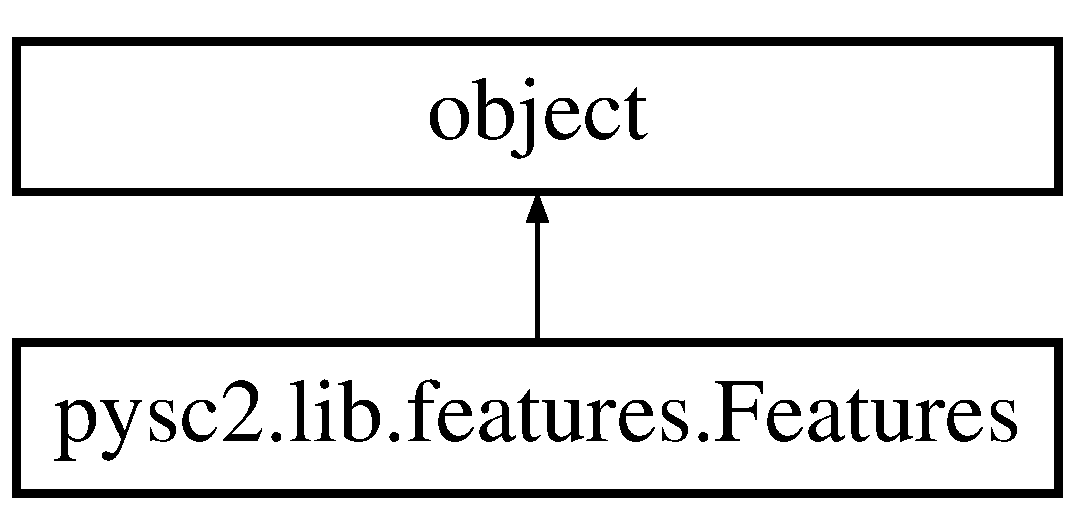
\includegraphics[height=2.000000cm]{classpysc2_1_1lib_1_1features_1_1_features}
\end{center}
\end{figure}
\subsection*{Public Member Functions}
\begin{DoxyCompactItemize}
\item 
def \mbox{\hyperlink{classpysc2_1_1lib_1_1features_1_1_features_af12dfcaae0adbc89c662a44b8ce762de}{\+\_\+\+\_\+init\+\_\+\+\_\+}} (self, agent\+\_\+interface\+\_\+format=None, map\+\_\+size=None)
\item 
def \mbox{\hyperlink{classpysc2_1_1lib_1_1features_1_1_features_a4b1d691f5d9376c1116a6c81a927e865}{observation\+\_\+spec}} (self)
\item 
def \mbox{\hyperlink{classpysc2_1_1lib_1_1features_1_1_features_a76e3d8bfc6e588ee9dddbbb34015ca7d}{action\+\_\+spec}} (self)
\item 
def \mbox{\hyperlink{classpysc2_1_1lib_1_1features_1_1_features_a79fe09a0d35b8d7b6f761da2ddc72f67}{transform\+\_\+obs}} (self, obs)
\item 
def \mbox{\hyperlink{classpysc2_1_1lib_1_1features_1_1_features_ad5a0a4cc33805616b7219e81d5be3d03}{available\+\_\+actions}} (self, obs)
\item 
def \mbox{\hyperlink{classpysc2_1_1lib_1_1features_1_1_features_a4d30783f71487ebbf7ac3cf21873af65}{transform\+\_\+action}} (self, obs, func\+\_\+call, skip\+\_\+available=False)
\item 
def \mbox{\hyperlink{classpysc2_1_1lib_1_1features_1_1_features_ae50848a35cd3c31833d1eb37662611f3}{reverse\+\_\+action}} (self, action)
\end{DoxyCompactItemize}


\subsection{Detailed Description}
\begin{DoxyVerb}Render feature layers from SC2 Observation protos into numpy arrays.

This has the implementation details of how to render a starcraft environment.
It translates between agent action/observation formats and starcraft
action/observation formats, which should not be seen by agent authors. The
starcraft protos contain more information than they should have access to.

This is outside of the environment so that it can also be used in other
contexts, eg a supervised dataset pipeline.
\end{DoxyVerb}
 

\subsection{Constructor \& Destructor Documentation}
\mbox{\Hypertarget{classpysc2_1_1lib_1_1features_1_1_features_af12dfcaae0adbc89c662a44b8ce762de}\label{classpysc2_1_1lib_1_1features_1_1_features_af12dfcaae0adbc89c662a44b8ce762de}} 
\index{pysc2\+::lib\+::features\+::\+Features@{pysc2\+::lib\+::features\+::\+Features}!\+\_\+\+\_\+init\+\_\+\+\_\+@{\+\_\+\+\_\+init\+\_\+\+\_\+}}
\index{\+\_\+\+\_\+init\+\_\+\+\_\+@{\+\_\+\+\_\+init\+\_\+\+\_\+}!pysc2\+::lib\+::features\+::\+Features@{pysc2\+::lib\+::features\+::\+Features}}
\subsubsection{\texorpdfstring{\+\_\+\+\_\+init\+\_\+\+\_\+()}{\_\_init\_\_()}}
{\footnotesize\ttfamily def pysc2.\+lib.\+features.\+Features.\+\_\+\+\_\+init\+\_\+\+\_\+ (\begin{DoxyParamCaption}\item[{}]{self,  }\item[{}]{agent\+\_\+interface\+\_\+format = {\ttfamily None},  }\item[{}]{map\+\_\+size = {\ttfamily None} }\end{DoxyParamCaption})}

\begin{DoxyVerb}Initialize a Features instance matching the specified interface format.

Args:
  agent_interface_format: See the documentation for `AgentInterfaceFormat`.
  map_size: The size of the map in world units, needed for feature_units.

Raises:
  ValueError: if agent_interface_format isn't specified.
  ValueError: if map_size isn't specified when use_feature_units is.
\end{DoxyVerb}
 

\subsection{Member Function Documentation}
\mbox{\Hypertarget{classpysc2_1_1lib_1_1features_1_1_features_a76e3d8bfc6e588ee9dddbbb34015ca7d}\label{classpysc2_1_1lib_1_1features_1_1_features_a76e3d8bfc6e588ee9dddbbb34015ca7d}} 
\index{pysc2\+::lib\+::features\+::\+Features@{pysc2\+::lib\+::features\+::\+Features}!action\+\_\+spec@{action\+\_\+spec}}
\index{action\+\_\+spec@{action\+\_\+spec}!pysc2\+::lib\+::features\+::\+Features@{pysc2\+::lib\+::features\+::\+Features}}
\subsubsection{\texorpdfstring{action\+\_\+spec()}{action\_spec()}}
{\footnotesize\ttfamily def pysc2.\+lib.\+features.\+Features.\+action\+\_\+spec (\begin{DoxyParamCaption}\item[{}]{self }\end{DoxyParamCaption})}

\begin{DoxyVerb}The action space pretty complicated and fills the ValidFunctions.\end{DoxyVerb}
 \mbox{\Hypertarget{classpysc2_1_1lib_1_1features_1_1_features_ad5a0a4cc33805616b7219e81d5be3d03}\label{classpysc2_1_1lib_1_1features_1_1_features_ad5a0a4cc33805616b7219e81d5be3d03}} 
\index{pysc2\+::lib\+::features\+::\+Features@{pysc2\+::lib\+::features\+::\+Features}!available\+\_\+actions@{available\+\_\+actions}}
\index{available\+\_\+actions@{available\+\_\+actions}!pysc2\+::lib\+::features\+::\+Features@{pysc2\+::lib\+::features\+::\+Features}}
\subsubsection{\texorpdfstring{available\+\_\+actions()}{available\_actions()}}
{\footnotesize\ttfamily def pysc2.\+lib.\+features.\+Features.\+available\+\_\+actions (\begin{DoxyParamCaption}\item[{}]{self,  }\item[{}]{obs }\end{DoxyParamCaption})}

\begin{DoxyVerb}Return the list of available action ids.\end{DoxyVerb}
 \mbox{\Hypertarget{classpysc2_1_1lib_1_1features_1_1_features_a4b1d691f5d9376c1116a6c81a927e865}\label{classpysc2_1_1lib_1_1features_1_1_features_a4b1d691f5d9376c1116a6c81a927e865}} 
\index{pysc2\+::lib\+::features\+::\+Features@{pysc2\+::lib\+::features\+::\+Features}!observation\+\_\+spec@{observation\+\_\+spec}}
\index{observation\+\_\+spec@{observation\+\_\+spec}!pysc2\+::lib\+::features\+::\+Features@{pysc2\+::lib\+::features\+::\+Features}}
\subsubsection{\texorpdfstring{observation\+\_\+spec()}{observation\_spec()}}
{\footnotesize\ttfamily def pysc2.\+lib.\+features.\+Features.\+observation\+\_\+spec (\begin{DoxyParamCaption}\item[{}]{self }\end{DoxyParamCaption})}

\begin{DoxyVerb}The observation spec for the SC2 environment.

It's worth noting that the image-like observations are in y,x/row,column
order which is different than the actions which are in x,y order. This is
due to conflicting conventions, and to facilitate printing of the images.

Returns:
  The dict of observation names to their tensor shapes. Shapes with a 0 can
  vary in length, for example the number of valid actions depends on which
  units you have selected.
\end{DoxyVerb}
 \mbox{\Hypertarget{classpysc2_1_1lib_1_1features_1_1_features_ae50848a35cd3c31833d1eb37662611f3}\label{classpysc2_1_1lib_1_1features_1_1_features_ae50848a35cd3c31833d1eb37662611f3}} 
\index{pysc2\+::lib\+::features\+::\+Features@{pysc2\+::lib\+::features\+::\+Features}!reverse\+\_\+action@{reverse\+\_\+action}}
\index{reverse\+\_\+action@{reverse\+\_\+action}!pysc2\+::lib\+::features\+::\+Features@{pysc2\+::lib\+::features\+::\+Features}}
\subsubsection{\texorpdfstring{reverse\+\_\+action()}{reverse\_action()}}
{\footnotesize\ttfamily def pysc2.\+lib.\+features.\+Features.\+reverse\+\_\+action (\begin{DoxyParamCaption}\item[{}]{self,  }\item[{}]{action }\end{DoxyParamCaption})}

\begin{DoxyVerb}Transform an SC2-style action into an agent-style action.

This should be the inverse of `transform_action`.

Args:
  action: a `sc_pb.Action` to be transformed.

Returns:
  A corresponding `actions.FunctionCall`.

Raises:
  ValueError: if it doesn't know how to transform this action.
\end{DoxyVerb}
 \mbox{\Hypertarget{classpysc2_1_1lib_1_1features_1_1_features_a4d30783f71487ebbf7ac3cf21873af65}\label{classpysc2_1_1lib_1_1features_1_1_features_a4d30783f71487ebbf7ac3cf21873af65}} 
\index{pysc2\+::lib\+::features\+::\+Features@{pysc2\+::lib\+::features\+::\+Features}!transform\+\_\+action@{transform\+\_\+action}}
\index{transform\+\_\+action@{transform\+\_\+action}!pysc2\+::lib\+::features\+::\+Features@{pysc2\+::lib\+::features\+::\+Features}}
\subsubsection{\texorpdfstring{transform\+\_\+action()}{transform\_action()}}
{\footnotesize\ttfamily def pysc2.\+lib.\+features.\+Features.\+transform\+\_\+action (\begin{DoxyParamCaption}\item[{}]{self,  }\item[{}]{obs,  }\item[{}]{func\+\_\+call,  }\item[{}]{skip\+\_\+available = {\ttfamily False} }\end{DoxyParamCaption})}

\begin{DoxyVerb}Tranform an agent-style action to one that SC2 can consume.

Args:
  obs: a `sc_pb.Observation` from the previous frame.
  func_call: a `FunctionCall` to be turned into a `sc_pb.Action`.
  skip_available: If True, assume the action is available. This should only
  be used for testing or if you expect to make actions that weren't
  valid at the last observation.

Returns:
  a corresponding `sc_pb.Action`.

Raises:
  ValueError: if the action doesn't pass validation.
\end{DoxyVerb}
 \mbox{\Hypertarget{classpysc2_1_1lib_1_1features_1_1_features_a79fe09a0d35b8d7b6f761da2ddc72f67}\label{classpysc2_1_1lib_1_1features_1_1_features_a79fe09a0d35b8d7b6f761da2ddc72f67}} 
\index{pysc2\+::lib\+::features\+::\+Features@{pysc2\+::lib\+::features\+::\+Features}!transform\+\_\+obs@{transform\+\_\+obs}}
\index{transform\+\_\+obs@{transform\+\_\+obs}!pysc2\+::lib\+::features\+::\+Features@{pysc2\+::lib\+::features\+::\+Features}}
\subsubsection{\texorpdfstring{transform\+\_\+obs()}{transform\_obs()}}
{\footnotesize\ttfamily def pysc2.\+lib.\+features.\+Features.\+transform\+\_\+obs (\begin{DoxyParamCaption}\item[{}]{self,  }\item[{}]{obs }\end{DoxyParamCaption})}

\begin{DoxyVerb}Render some SC2 observations into something an agent can handle.\end{DoxyVerb}
 

The documentation for this class was generated from the following file\+:\begin{DoxyCompactItemize}
\item 
lib/\mbox{\hyperlink{features_8py}{features.\+py}}\end{DoxyCompactItemize}

\hypertarget{classpysc2_1_1lib_1_1features__test_1_1_features_test}{}\section{pysc2.\+lib.\+features\+\_\+test.\+Features\+Test Class Reference}
\label{classpysc2_1_1lib_1_1features__test_1_1_features_test}\index{pysc2.\+lib.\+features\+\_\+test.\+Features\+Test@{pysc2.\+lib.\+features\+\_\+test.\+Features\+Test}}
Inheritance diagram for pysc2.\+lib.\+features\+\_\+test.\+Features\+Test\+:\begin{figure}[H]
\begin{center}
\leavevmode
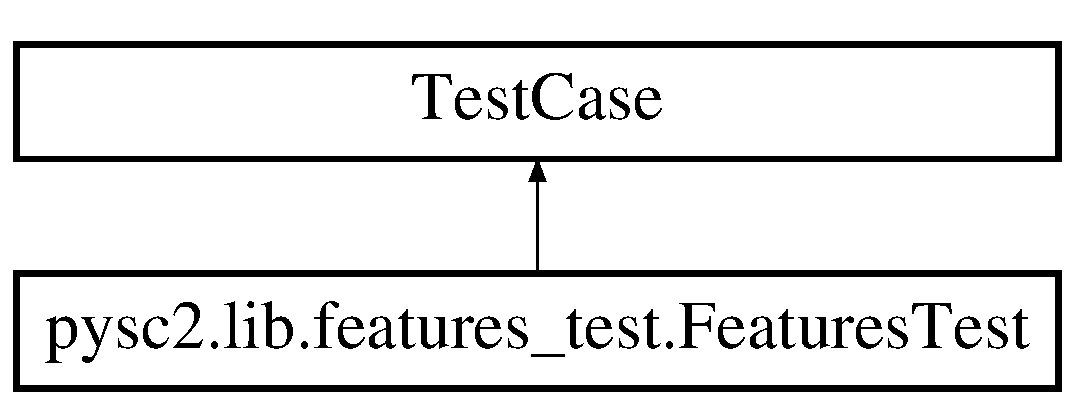
\includegraphics[height=2.000000cm]{classpysc2_1_1lib_1_1features__test_1_1_features_test}
\end{center}
\end{figure}
\subsection*{Public Member Functions}
\begin{DoxyCompactItemize}
\item 
def \mbox{\hyperlink{classpysc2_1_1lib_1_1features__test_1_1_features_test_ae155ba0432bbdf3c0637edde339a4bf3}{test\+Functions\+Ids\+Are\+Consistent}} (self)
\item 
def \mbox{\hyperlink{classpysc2_1_1lib_1_1features__test_1_1_features_test_a9caf3659f3783bd5cb55e47fea09fdf4}{test\+All\+Versions\+Of\+An\+Ability\+Have\+The\+Same\+General}} (self)
\item 
def \mbox{\hyperlink{classpysc2_1_1lib_1_1features__test_1_1_features_test_a174e0178a227e367c212dc99de396dab}{test\+Valid\+Functions\+Are\+Consistent}} (self)
\item 
def \mbox{\hyperlink{classpysc2_1_1lib_1_1features__test_1_1_features_test_af14dc6f548faff56839d0b6d2ffb0af9}{gen\+\_\+random\+\_\+function\+\_\+call}} (self, action\+\_\+spec, func\+\_\+id)
\item 
def \mbox{\hyperlink{classpysc2_1_1lib_1_1features__test_1_1_features_test_a4e3f221ce65b9d51eab877ba66bd8c9a}{test\+Ids\+Match\+Index}} (self)
\item 
def \mbox{\hyperlink{classpysc2_1_1lib_1_1features__test_1_1_features_test_ad4095c1ac9fa6ecfa7b0824eeb39972a}{test\+Reversing\+Unknown\+Action}} (self)
\item 
def \mbox{\hyperlink{classpysc2_1_1lib_1_1features__test_1_1_features_test_a47c11cce3301e4e196d58febbbfdca1b}{test\+Specific\+Actions\+Are\+Reversible}} (self)
\item 
def \mbox{\hyperlink{classpysc2_1_1lib_1_1features__test_1_1_features_test_aaa465371eb5f843df3b7d0b8b7b8e3c1}{test\+Can\+Pickle\+Specs}} (self)
\item 
def \mbox{\hyperlink{classpysc2_1_1lib_1_1features__test_1_1_features_test_a9dfbb6050949524fbe9eaddc307c60a9}{test\+Can\+Pickle\+Function\+Call}} (self)
\item 
def \mbox{\hyperlink{classpysc2_1_1lib_1_1features__test_1_1_features_test_aabcdc707b4f55ce05986959787f034c1}{test\+Can\+Deepcopy\+Numpy\+Function\+Call}} (self)
\item 
def \mbox{\hyperlink{classpysc2_1_1lib_1_1features__test_1_1_features_test_a55941b95526a89d67c4f1ac577bc6cac}{test\+Size\+Constructors}} (self)
\item 
def \mbox{\hyperlink{classpysc2_1_1lib_1_1features__test_1_1_features_test_abd061b800bbe5cc61f11740d27411fb4}{test\+Fl\+Rgb\+Action\+Spec}} (self)
\item 
def \mbox{\hyperlink{classpysc2_1_1lib_1_1features__test_1_1_features_test_a9b48fdd9a34b1891d18561867d4cd7a8}{test\+Fl\+Rgb\+Observation\+Spec}} (self)
\end{DoxyCompactItemize}


\subsection{Member Function Documentation}
\mbox{\Hypertarget{classpysc2_1_1lib_1_1features__test_1_1_features_test_af14dc6f548faff56839d0b6d2ffb0af9}\label{classpysc2_1_1lib_1_1features__test_1_1_features_test_af14dc6f548faff56839d0b6d2ffb0af9}} 
\index{pysc2\+::lib\+::features\+\_\+test\+::\+Features\+Test@{pysc2\+::lib\+::features\+\_\+test\+::\+Features\+Test}!gen\+\_\+random\+\_\+function\+\_\+call@{gen\+\_\+random\+\_\+function\+\_\+call}}
\index{gen\+\_\+random\+\_\+function\+\_\+call@{gen\+\_\+random\+\_\+function\+\_\+call}!pysc2\+::lib\+::features\+\_\+test\+::\+Features\+Test@{pysc2\+::lib\+::features\+\_\+test\+::\+Features\+Test}}
\subsubsection{\texorpdfstring{gen\+\_\+random\+\_\+function\+\_\+call()}{gen\_random\_function\_call()}}
{\footnotesize\ttfamily def pysc2.\+lib.\+features\+\_\+test.\+Features\+Test.\+gen\+\_\+random\+\_\+function\+\_\+call (\begin{DoxyParamCaption}\item[{}]{self,  }\item[{}]{action\+\_\+spec,  }\item[{}]{func\+\_\+id }\end{DoxyParamCaption})}

\mbox{\Hypertarget{classpysc2_1_1lib_1_1features__test_1_1_features_test_a9caf3659f3783bd5cb55e47fea09fdf4}\label{classpysc2_1_1lib_1_1features__test_1_1_features_test_a9caf3659f3783bd5cb55e47fea09fdf4}} 
\index{pysc2\+::lib\+::features\+\_\+test\+::\+Features\+Test@{pysc2\+::lib\+::features\+\_\+test\+::\+Features\+Test}!test\+All\+Versions\+Of\+An\+Ability\+Have\+The\+Same\+General@{test\+All\+Versions\+Of\+An\+Ability\+Have\+The\+Same\+General}}
\index{test\+All\+Versions\+Of\+An\+Ability\+Have\+The\+Same\+General@{test\+All\+Versions\+Of\+An\+Ability\+Have\+The\+Same\+General}!pysc2\+::lib\+::features\+\_\+test\+::\+Features\+Test@{pysc2\+::lib\+::features\+\_\+test\+::\+Features\+Test}}
\subsubsection{\texorpdfstring{test\+All\+Versions\+Of\+An\+Ability\+Have\+The\+Same\+General()}{testAllVersionsOfAnAbilityHaveTheSameGeneral()}}
{\footnotesize\ttfamily def pysc2.\+lib.\+features\+\_\+test.\+Features\+Test.\+test\+All\+Versions\+Of\+An\+Ability\+Have\+The\+Same\+General (\begin{DoxyParamCaption}\item[{}]{self }\end{DoxyParamCaption})}

\mbox{\Hypertarget{classpysc2_1_1lib_1_1features__test_1_1_features_test_aabcdc707b4f55ce05986959787f034c1}\label{classpysc2_1_1lib_1_1features__test_1_1_features_test_aabcdc707b4f55ce05986959787f034c1}} 
\index{pysc2\+::lib\+::features\+\_\+test\+::\+Features\+Test@{pysc2\+::lib\+::features\+\_\+test\+::\+Features\+Test}!test\+Can\+Deepcopy\+Numpy\+Function\+Call@{test\+Can\+Deepcopy\+Numpy\+Function\+Call}}
\index{test\+Can\+Deepcopy\+Numpy\+Function\+Call@{test\+Can\+Deepcopy\+Numpy\+Function\+Call}!pysc2\+::lib\+::features\+\_\+test\+::\+Features\+Test@{pysc2\+::lib\+::features\+\_\+test\+::\+Features\+Test}}
\subsubsection{\texorpdfstring{test\+Can\+Deepcopy\+Numpy\+Function\+Call()}{testCanDeepcopyNumpyFunctionCall()}}
{\footnotesize\ttfamily def pysc2.\+lib.\+features\+\_\+test.\+Features\+Test.\+test\+Can\+Deepcopy\+Numpy\+Function\+Call (\begin{DoxyParamCaption}\item[{}]{self }\end{DoxyParamCaption})}

\mbox{\Hypertarget{classpysc2_1_1lib_1_1features__test_1_1_features_test_a9dfbb6050949524fbe9eaddc307c60a9}\label{classpysc2_1_1lib_1_1features__test_1_1_features_test_a9dfbb6050949524fbe9eaddc307c60a9}} 
\index{pysc2\+::lib\+::features\+\_\+test\+::\+Features\+Test@{pysc2\+::lib\+::features\+\_\+test\+::\+Features\+Test}!test\+Can\+Pickle\+Function\+Call@{test\+Can\+Pickle\+Function\+Call}}
\index{test\+Can\+Pickle\+Function\+Call@{test\+Can\+Pickle\+Function\+Call}!pysc2\+::lib\+::features\+\_\+test\+::\+Features\+Test@{pysc2\+::lib\+::features\+\_\+test\+::\+Features\+Test}}
\subsubsection{\texorpdfstring{test\+Can\+Pickle\+Function\+Call()}{testCanPickleFunctionCall()}}
{\footnotesize\ttfamily def pysc2.\+lib.\+features\+\_\+test.\+Features\+Test.\+test\+Can\+Pickle\+Function\+Call (\begin{DoxyParamCaption}\item[{}]{self }\end{DoxyParamCaption})}

\mbox{\Hypertarget{classpysc2_1_1lib_1_1features__test_1_1_features_test_aaa465371eb5f843df3b7d0b8b7b8e3c1}\label{classpysc2_1_1lib_1_1features__test_1_1_features_test_aaa465371eb5f843df3b7d0b8b7b8e3c1}} 
\index{pysc2\+::lib\+::features\+\_\+test\+::\+Features\+Test@{pysc2\+::lib\+::features\+\_\+test\+::\+Features\+Test}!test\+Can\+Pickle\+Specs@{test\+Can\+Pickle\+Specs}}
\index{test\+Can\+Pickle\+Specs@{test\+Can\+Pickle\+Specs}!pysc2\+::lib\+::features\+\_\+test\+::\+Features\+Test@{pysc2\+::lib\+::features\+\_\+test\+::\+Features\+Test}}
\subsubsection{\texorpdfstring{test\+Can\+Pickle\+Specs()}{testCanPickleSpecs()}}
{\footnotesize\ttfamily def pysc2.\+lib.\+features\+\_\+test.\+Features\+Test.\+test\+Can\+Pickle\+Specs (\begin{DoxyParamCaption}\item[{}]{self }\end{DoxyParamCaption})}

\mbox{\Hypertarget{classpysc2_1_1lib_1_1features__test_1_1_features_test_abd061b800bbe5cc61f11740d27411fb4}\label{classpysc2_1_1lib_1_1features__test_1_1_features_test_abd061b800bbe5cc61f11740d27411fb4}} 
\index{pysc2\+::lib\+::features\+\_\+test\+::\+Features\+Test@{pysc2\+::lib\+::features\+\_\+test\+::\+Features\+Test}!test\+Fl\+Rgb\+Action\+Spec@{test\+Fl\+Rgb\+Action\+Spec}}
\index{test\+Fl\+Rgb\+Action\+Spec@{test\+Fl\+Rgb\+Action\+Spec}!pysc2\+::lib\+::features\+\_\+test\+::\+Features\+Test@{pysc2\+::lib\+::features\+\_\+test\+::\+Features\+Test}}
\subsubsection{\texorpdfstring{test\+Fl\+Rgb\+Action\+Spec()}{testFlRgbActionSpec()}}
{\footnotesize\ttfamily def pysc2.\+lib.\+features\+\_\+test.\+Features\+Test.\+test\+Fl\+Rgb\+Action\+Spec (\begin{DoxyParamCaption}\item[{}]{self }\end{DoxyParamCaption})}

\mbox{\Hypertarget{classpysc2_1_1lib_1_1features__test_1_1_features_test_a9b48fdd9a34b1891d18561867d4cd7a8}\label{classpysc2_1_1lib_1_1features__test_1_1_features_test_a9b48fdd9a34b1891d18561867d4cd7a8}} 
\index{pysc2\+::lib\+::features\+\_\+test\+::\+Features\+Test@{pysc2\+::lib\+::features\+\_\+test\+::\+Features\+Test}!test\+Fl\+Rgb\+Observation\+Spec@{test\+Fl\+Rgb\+Observation\+Spec}}
\index{test\+Fl\+Rgb\+Observation\+Spec@{test\+Fl\+Rgb\+Observation\+Spec}!pysc2\+::lib\+::features\+\_\+test\+::\+Features\+Test@{pysc2\+::lib\+::features\+\_\+test\+::\+Features\+Test}}
\subsubsection{\texorpdfstring{test\+Fl\+Rgb\+Observation\+Spec()}{testFlRgbObservationSpec()}}
{\footnotesize\ttfamily def pysc2.\+lib.\+features\+\_\+test.\+Features\+Test.\+test\+Fl\+Rgb\+Observation\+Spec (\begin{DoxyParamCaption}\item[{}]{self }\end{DoxyParamCaption})}

\mbox{\Hypertarget{classpysc2_1_1lib_1_1features__test_1_1_features_test_ae155ba0432bbdf3c0637edde339a4bf3}\label{classpysc2_1_1lib_1_1features__test_1_1_features_test_ae155ba0432bbdf3c0637edde339a4bf3}} 
\index{pysc2\+::lib\+::features\+\_\+test\+::\+Features\+Test@{pysc2\+::lib\+::features\+\_\+test\+::\+Features\+Test}!test\+Functions\+Ids\+Are\+Consistent@{test\+Functions\+Ids\+Are\+Consistent}}
\index{test\+Functions\+Ids\+Are\+Consistent@{test\+Functions\+Ids\+Are\+Consistent}!pysc2\+::lib\+::features\+\_\+test\+::\+Features\+Test@{pysc2\+::lib\+::features\+\_\+test\+::\+Features\+Test}}
\subsubsection{\texorpdfstring{test\+Functions\+Ids\+Are\+Consistent()}{testFunctionsIdsAreConsistent()}}
{\footnotesize\ttfamily def pysc2.\+lib.\+features\+\_\+test.\+Features\+Test.\+test\+Functions\+Ids\+Are\+Consistent (\begin{DoxyParamCaption}\item[{}]{self }\end{DoxyParamCaption})}

\mbox{\Hypertarget{classpysc2_1_1lib_1_1features__test_1_1_features_test_a4e3f221ce65b9d51eab877ba66bd8c9a}\label{classpysc2_1_1lib_1_1features__test_1_1_features_test_a4e3f221ce65b9d51eab877ba66bd8c9a}} 
\index{pysc2\+::lib\+::features\+\_\+test\+::\+Features\+Test@{pysc2\+::lib\+::features\+\_\+test\+::\+Features\+Test}!test\+Ids\+Match\+Index@{test\+Ids\+Match\+Index}}
\index{test\+Ids\+Match\+Index@{test\+Ids\+Match\+Index}!pysc2\+::lib\+::features\+\_\+test\+::\+Features\+Test@{pysc2\+::lib\+::features\+\_\+test\+::\+Features\+Test}}
\subsubsection{\texorpdfstring{test\+Ids\+Match\+Index()}{testIdsMatchIndex()}}
{\footnotesize\ttfamily def pysc2.\+lib.\+features\+\_\+test.\+Features\+Test.\+test\+Ids\+Match\+Index (\begin{DoxyParamCaption}\item[{}]{self }\end{DoxyParamCaption})}

\mbox{\Hypertarget{classpysc2_1_1lib_1_1features__test_1_1_features_test_ad4095c1ac9fa6ecfa7b0824eeb39972a}\label{classpysc2_1_1lib_1_1features__test_1_1_features_test_ad4095c1ac9fa6ecfa7b0824eeb39972a}} 
\index{pysc2\+::lib\+::features\+\_\+test\+::\+Features\+Test@{pysc2\+::lib\+::features\+\_\+test\+::\+Features\+Test}!test\+Reversing\+Unknown\+Action@{test\+Reversing\+Unknown\+Action}}
\index{test\+Reversing\+Unknown\+Action@{test\+Reversing\+Unknown\+Action}!pysc2\+::lib\+::features\+\_\+test\+::\+Features\+Test@{pysc2\+::lib\+::features\+\_\+test\+::\+Features\+Test}}
\subsubsection{\texorpdfstring{test\+Reversing\+Unknown\+Action()}{testReversingUnknownAction()}}
{\footnotesize\ttfamily def pysc2.\+lib.\+features\+\_\+test.\+Features\+Test.\+test\+Reversing\+Unknown\+Action (\begin{DoxyParamCaption}\item[{}]{self }\end{DoxyParamCaption})}

\mbox{\Hypertarget{classpysc2_1_1lib_1_1features__test_1_1_features_test_a55941b95526a89d67c4f1ac577bc6cac}\label{classpysc2_1_1lib_1_1features__test_1_1_features_test_a55941b95526a89d67c4f1ac577bc6cac}} 
\index{pysc2\+::lib\+::features\+\_\+test\+::\+Features\+Test@{pysc2\+::lib\+::features\+\_\+test\+::\+Features\+Test}!test\+Size\+Constructors@{test\+Size\+Constructors}}
\index{test\+Size\+Constructors@{test\+Size\+Constructors}!pysc2\+::lib\+::features\+\_\+test\+::\+Features\+Test@{pysc2\+::lib\+::features\+\_\+test\+::\+Features\+Test}}
\subsubsection{\texorpdfstring{test\+Size\+Constructors()}{testSizeConstructors()}}
{\footnotesize\ttfamily def pysc2.\+lib.\+features\+\_\+test.\+Features\+Test.\+test\+Size\+Constructors (\begin{DoxyParamCaption}\item[{}]{self }\end{DoxyParamCaption})}

\mbox{\Hypertarget{classpysc2_1_1lib_1_1features__test_1_1_features_test_a47c11cce3301e4e196d58febbbfdca1b}\label{classpysc2_1_1lib_1_1features__test_1_1_features_test_a47c11cce3301e4e196d58febbbfdca1b}} 
\index{pysc2\+::lib\+::features\+\_\+test\+::\+Features\+Test@{pysc2\+::lib\+::features\+\_\+test\+::\+Features\+Test}!test\+Specific\+Actions\+Are\+Reversible@{test\+Specific\+Actions\+Are\+Reversible}}
\index{test\+Specific\+Actions\+Are\+Reversible@{test\+Specific\+Actions\+Are\+Reversible}!pysc2\+::lib\+::features\+\_\+test\+::\+Features\+Test@{pysc2\+::lib\+::features\+\_\+test\+::\+Features\+Test}}
\subsubsection{\texorpdfstring{test\+Specific\+Actions\+Are\+Reversible()}{testSpecificActionsAreReversible()}}
{\footnotesize\ttfamily def pysc2.\+lib.\+features\+\_\+test.\+Features\+Test.\+test\+Specific\+Actions\+Are\+Reversible (\begin{DoxyParamCaption}\item[{}]{self }\end{DoxyParamCaption})}

\begin{DoxyVerb}Test that the `transform_action` and `reverse_action` are inverses.\end{DoxyVerb}
 \mbox{\Hypertarget{classpysc2_1_1lib_1_1features__test_1_1_features_test_a174e0178a227e367c212dc99de396dab}\label{classpysc2_1_1lib_1_1features__test_1_1_features_test_a174e0178a227e367c212dc99de396dab}} 
\index{pysc2\+::lib\+::features\+\_\+test\+::\+Features\+Test@{pysc2\+::lib\+::features\+\_\+test\+::\+Features\+Test}!test\+Valid\+Functions\+Are\+Consistent@{test\+Valid\+Functions\+Are\+Consistent}}
\index{test\+Valid\+Functions\+Are\+Consistent@{test\+Valid\+Functions\+Are\+Consistent}!pysc2\+::lib\+::features\+\_\+test\+::\+Features\+Test@{pysc2\+::lib\+::features\+\_\+test\+::\+Features\+Test}}
\subsubsection{\texorpdfstring{test\+Valid\+Functions\+Are\+Consistent()}{testValidFunctionsAreConsistent()}}
{\footnotesize\ttfamily def pysc2.\+lib.\+features\+\_\+test.\+Features\+Test.\+test\+Valid\+Functions\+Are\+Consistent (\begin{DoxyParamCaption}\item[{}]{self }\end{DoxyParamCaption})}



The documentation for this class was generated from the following file\+:\begin{DoxyCompactItemize}
\item 
lib/\mbox{\hyperlink{features__test_8py}{features\+\_\+test.\+py}}\end{DoxyCompactItemize}

\hypertarget{classpysc2_1_1lib_1_1features_1_1_feature_type}{}\section{pysc2.\+lib.\+features.\+Feature\+Type Class Reference}
\label{classpysc2_1_1lib_1_1features_1_1_feature_type}\index{pysc2.\+lib.\+features.\+Feature\+Type@{pysc2.\+lib.\+features.\+Feature\+Type}}
Inheritance diagram for pysc2.\+lib.\+features.\+Feature\+Type\+:\begin{figure}[H]
\begin{center}
\leavevmode
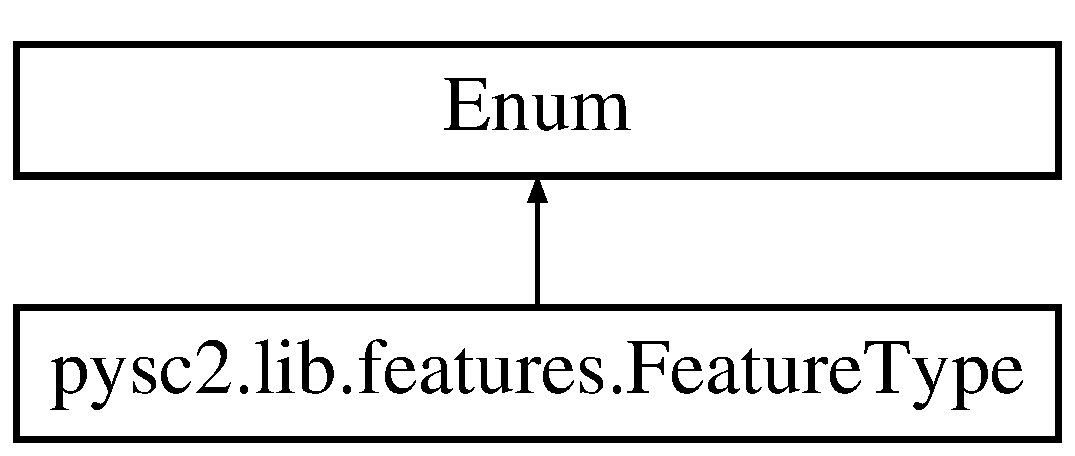
\includegraphics[height=2.000000cm]{classpysc2_1_1lib_1_1features_1_1_feature_type}
\end{center}
\end{figure}
\subsection*{Static Public Attributes}
\begin{DoxyCompactItemize}
\item 
int \mbox{\hyperlink{classpysc2_1_1lib_1_1features_1_1_feature_type_a337be9da5251eee1cade6521de9aae6b}{S\+C\+A\+L\+AR}} = 1
\item 
int \mbox{\hyperlink{classpysc2_1_1lib_1_1features_1_1_feature_type_a8949fad00934fe5c01fc1fe471160919}{C\+A\+T\+E\+G\+O\+R\+I\+C\+AL}} = 2
\end{DoxyCompactItemize}


\subsection{Member Data Documentation}
\mbox{\Hypertarget{classpysc2_1_1lib_1_1features_1_1_feature_type_a8949fad00934fe5c01fc1fe471160919}\label{classpysc2_1_1lib_1_1features_1_1_feature_type_a8949fad00934fe5c01fc1fe471160919}} 
\index{pysc2\+::lib\+::features\+::\+Feature\+Type@{pysc2\+::lib\+::features\+::\+Feature\+Type}!C\+A\+T\+E\+G\+O\+R\+I\+C\+AL@{C\+A\+T\+E\+G\+O\+R\+I\+C\+AL}}
\index{C\+A\+T\+E\+G\+O\+R\+I\+C\+AL@{C\+A\+T\+E\+G\+O\+R\+I\+C\+AL}!pysc2\+::lib\+::features\+::\+Feature\+Type@{pysc2\+::lib\+::features\+::\+Feature\+Type}}
\subsubsection{\texorpdfstring{C\+A\+T\+E\+G\+O\+R\+I\+C\+AL}{CATEGORICAL}}
{\footnotesize\ttfamily int pysc2.\+lib.\+features.\+Feature\+Type.\+C\+A\+T\+E\+G\+O\+R\+I\+C\+AL = 2\hspace{0.3cm}{\ttfamily [static]}}

\mbox{\Hypertarget{classpysc2_1_1lib_1_1features_1_1_feature_type_a337be9da5251eee1cade6521de9aae6b}\label{classpysc2_1_1lib_1_1features_1_1_feature_type_a337be9da5251eee1cade6521de9aae6b}} 
\index{pysc2\+::lib\+::features\+::\+Feature\+Type@{pysc2\+::lib\+::features\+::\+Feature\+Type}!S\+C\+A\+L\+AR@{S\+C\+A\+L\+AR}}
\index{S\+C\+A\+L\+AR@{S\+C\+A\+L\+AR}!pysc2\+::lib\+::features\+::\+Feature\+Type@{pysc2\+::lib\+::features\+::\+Feature\+Type}}
\subsubsection{\texorpdfstring{S\+C\+A\+L\+AR}{SCALAR}}
{\footnotesize\ttfamily int pysc2.\+lib.\+features.\+Feature\+Type.\+S\+C\+A\+L\+AR = 1\hspace{0.3cm}{\ttfamily [static]}}



The documentation for this class was generated from the following file\+:\begin{DoxyCompactItemize}
\item 
lib/\mbox{\hyperlink{features_8py}{features.\+py}}\end{DoxyCompactItemize}

\hypertarget{classpysc2_1_1lib_1_1features_1_1_feature_unit}{}\section{pysc2.\+lib.\+features.\+Feature\+Unit Class Reference}
\label{classpysc2_1_1lib_1_1features_1_1_feature_unit}\index{pysc2.\+lib.\+features.\+Feature\+Unit@{pysc2.\+lib.\+features.\+Feature\+Unit}}
Inheritance diagram for pysc2.\+lib.\+features.\+Feature\+Unit\+:\begin{figure}[H]
\begin{center}
\leavevmode
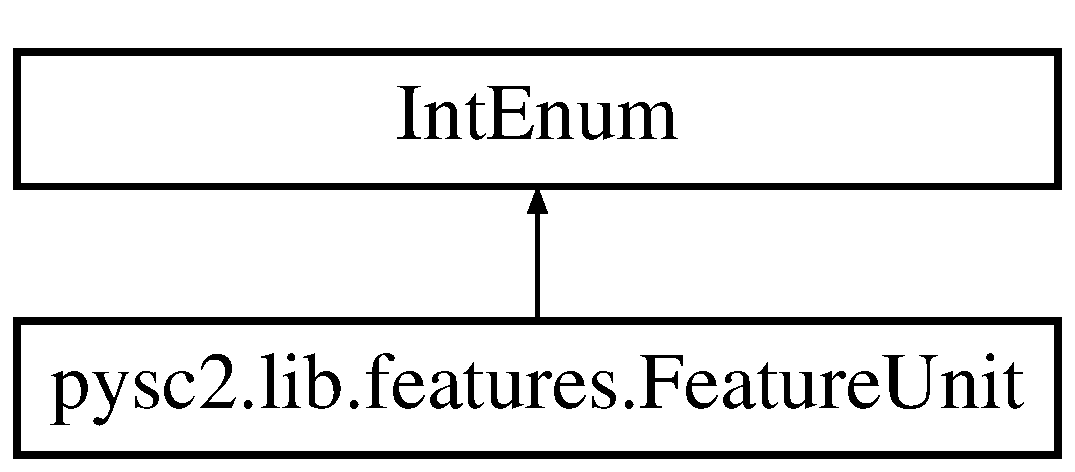
\includegraphics[height=2.000000cm]{classpysc2_1_1lib_1_1features_1_1_feature_unit}
\end{center}
\end{figure}
\subsection*{Static Public Attributes}
\begin{DoxyCompactItemize}
\item 
int \mbox{\hyperlink{classpysc2_1_1lib_1_1features_1_1_feature_unit_a984d41a1fb3501844c91f06db01df36e}{unit\+\_\+type}} = 0
\item 
int \mbox{\hyperlink{classpysc2_1_1lib_1_1features_1_1_feature_unit_a1851bf7e1192818d533104abefb9bebe}{alliance}} = 1
\item 
int \mbox{\hyperlink{classpysc2_1_1lib_1_1features_1_1_feature_unit_a0ae8311cdeac1c2e6a2c8054884884bf}{health}} = 2
\item 
int \mbox{\hyperlink{classpysc2_1_1lib_1_1features_1_1_feature_unit_a74785179227770fa126f8c2711731cd2}{shield}} = 3
\item 
int \mbox{\hyperlink{classpysc2_1_1lib_1_1features_1_1_feature_unit_abd505bf044c3a0e9dbc0b706b55c52b9}{energy}} = 4
\item 
int \mbox{\hyperlink{classpysc2_1_1lib_1_1features_1_1_feature_unit_ab4efafc4a507de84958c06911238097b}{cargo\+\_\+space\+\_\+taken}} = 5
\item 
int \mbox{\hyperlink{classpysc2_1_1lib_1_1features_1_1_feature_unit_a44d315908a65730ac43e35a2788bba34}{build\+\_\+progress}} = 6
\item 
int \mbox{\hyperlink{classpysc2_1_1lib_1_1features_1_1_feature_unit_a3e572b847d1be4468461f1859b30f237}{health\+\_\+ratio}} = 7
\item 
int \mbox{\hyperlink{classpysc2_1_1lib_1_1features_1_1_feature_unit_a603ea33bd99e5bc81bcc6c0329301830}{shield\+\_\+ratio}} = 8
\item 
int \mbox{\hyperlink{classpysc2_1_1lib_1_1features_1_1_feature_unit_a67bb060d4d31601806053ff3d7a2e463}{energy\+\_\+ratio}} = 9
\item 
int \mbox{\hyperlink{classpysc2_1_1lib_1_1features_1_1_feature_unit_acdac6d62f36fc9623ba2ea2cd328ea8f}{display\+\_\+type}} = 10
\item 
int \mbox{\hyperlink{classpysc2_1_1lib_1_1features_1_1_feature_unit_af878a27434fcd99e7714eacda482087f}{owner}} = 11
\item 
int \mbox{\hyperlink{classpysc2_1_1lib_1_1features_1_1_feature_unit_ad947e850a2efadb4d6e4b6347574f260}{x}} = 12
\item 
int \mbox{\hyperlink{classpysc2_1_1lib_1_1features_1_1_feature_unit_a450e6fffdc395bc7b3809aa5ecf8c550}{y}} = 13
\item 
int \mbox{\hyperlink{classpysc2_1_1lib_1_1features_1_1_feature_unit_a45067cf8a883cd2233ba0462565890a2}{facing}} = 14
\item 
int \mbox{\hyperlink{classpysc2_1_1lib_1_1features_1_1_feature_unit_a9b25b2fc95c9397202c1e7912cb63320}{radius}} = 15
\item 
int \mbox{\hyperlink{classpysc2_1_1lib_1_1features_1_1_feature_unit_a21224cb1c4d2caabdcc9806cd59a02cb}{cloak}} = 16
\item 
int \mbox{\hyperlink{classpysc2_1_1lib_1_1features_1_1_feature_unit_a64bce8f6b2d9f64bf4a372f5aa6cf220}{is\+\_\+selected}} = 17
\item 
int \mbox{\hyperlink{classpysc2_1_1lib_1_1features_1_1_feature_unit_a3dbaac94007fad92391a89a2bc4190cc}{is\+\_\+blip}} = 18
\item 
int \mbox{\hyperlink{classpysc2_1_1lib_1_1features_1_1_feature_unit_a905c1fab12f9fb2c3cfe564d63fd8ba0}{is\+\_\+powered}} = 19
\item 
int \mbox{\hyperlink{classpysc2_1_1lib_1_1features_1_1_feature_unit_a92bb15e577996b56367e18a5eade17c7}{mineral\+\_\+contents}} = 20
\item 
int \mbox{\hyperlink{classpysc2_1_1lib_1_1features_1_1_feature_unit_a351e5ddcbd5c0f193846c37757d2ea5e}{vespene\+\_\+contents}} = 21
\item 
int \mbox{\hyperlink{classpysc2_1_1lib_1_1features_1_1_feature_unit_a7ed363d7533c5e87093934c9e8d95d56}{cargo\+\_\+space\+\_\+max}} = 22
\item 
int \mbox{\hyperlink{classpysc2_1_1lib_1_1features_1_1_feature_unit_aad54c92e27aa800d72f03170ad0bb57c}{assigned\+\_\+harvesters}} = 23
\item 
int \mbox{\hyperlink{classpysc2_1_1lib_1_1features_1_1_feature_unit_ae768c5813efa8a31ee72fffb3cb51e6f}{ideal\+\_\+harvesters}} = 24
\item 
int \mbox{\hyperlink{classpysc2_1_1lib_1_1features_1_1_feature_unit_aa7f016cfc4f741c5998152568f1293d8}{weapon\+\_\+cooldown}} = 25
\end{DoxyCompactItemize}


\subsection{Detailed Description}
\begin{DoxyVerb}Indices for the `feature_unit` observations.\end{DoxyVerb}
 

\subsection{Member Data Documentation}
\mbox{\Hypertarget{classpysc2_1_1lib_1_1features_1_1_feature_unit_a1851bf7e1192818d533104abefb9bebe}\label{classpysc2_1_1lib_1_1features_1_1_feature_unit_a1851bf7e1192818d533104abefb9bebe}} 
\index{pysc2\+::lib\+::features\+::\+Feature\+Unit@{pysc2\+::lib\+::features\+::\+Feature\+Unit}!alliance@{alliance}}
\index{alliance@{alliance}!pysc2\+::lib\+::features\+::\+Feature\+Unit@{pysc2\+::lib\+::features\+::\+Feature\+Unit}}
\subsubsection{\texorpdfstring{alliance}{alliance}}
{\footnotesize\ttfamily int pysc2.\+lib.\+features.\+Feature\+Unit.\+alliance = 1\hspace{0.3cm}{\ttfamily [static]}}

\mbox{\Hypertarget{classpysc2_1_1lib_1_1features_1_1_feature_unit_aad54c92e27aa800d72f03170ad0bb57c}\label{classpysc2_1_1lib_1_1features_1_1_feature_unit_aad54c92e27aa800d72f03170ad0bb57c}} 
\index{pysc2\+::lib\+::features\+::\+Feature\+Unit@{pysc2\+::lib\+::features\+::\+Feature\+Unit}!assigned\+\_\+harvesters@{assigned\+\_\+harvesters}}
\index{assigned\+\_\+harvesters@{assigned\+\_\+harvesters}!pysc2\+::lib\+::features\+::\+Feature\+Unit@{pysc2\+::lib\+::features\+::\+Feature\+Unit}}
\subsubsection{\texorpdfstring{assigned\+\_\+harvesters}{assigned\_harvesters}}
{\footnotesize\ttfamily int pysc2.\+lib.\+features.\+Feature\+Unit.\+assigned\+\_\+harvesters = 23\hspace{0.3cm}{\ttfamily [static]}}

\mbox{\Hypertarget{classpysc2_1_1lib_1_1features_1_1_feature_unit_a44d315908a65730ac43e35a2788bba34}\label{classpysc2_1_1lib_1_1features_1_1_feature_unit_a44d315908a65730ac43e35a2788bba34}} 
\index{pysc2\+::lib\+::features\+::\+Feature\+Unit@{pysc2\+::lib\+::features\+::\+Feature\+Unit}!build\+\_\+progress@{build\+\_\+progress}}
\index{build\+\_\+progress@{build\+\_\+progress}!pysc2\+::lib\+::features\+::\+Feature\+Unit@{pysc2\+::lib\+::features\+::\+Feature\+Unit}}
\subsubsection{\texorpdfstring{build\+\_\+progress}{build\_progress}}
{\footnotesize\ttfamily int pysc2.\+lib.\+features.\+Feature\+Unit.\+build\+\_\+progress = 6\hspace{0.3cm}{\ttfamily [static]}}

\mbox{\Hypertarget{classpysc2_1_1lib_1_1features_1_1_feature_unit_a7ed363d7533c5e87093934c9e8d95d56}\label{classpysc2_1_1lib_1_1features_1_1_feature_unit_a7ed363d7533c5e87093934c9e8d95d56}} 
\index{pysc2\+::lib\+::features\+::\+Feature\+Unit@{pysc2\+::lib\+::features\+::\+Feature\+Unit}!cargo\+\_\+space\+\_\+max@{cargo\+\_\+space\+\_\+max}}
\index{cargo\+\_\+space\+\_\+max@{cargo\+\_\+space\+\_\+max}!pysc2\+::lib\+::features\+::\+Feature\+Unit@{pysc2\+::lib\+::features\+::\+Feature\+Unit}}
\subsubsection{\texorpdfstring{cargo\+\_\+space\+\_\+max}{cargo\_space\_max}}
{\footnotesize\ttfamily int pysc2.\+lib.\+features.\+Feature\+Unit.\+cargo\+\_\+space\+\_\+max = 22\hspace{0.3cm}{\ttfamily [static]}}

\mbox{\Hypertarget{classpysc2_1_1lib_1_1features_1_1_feature_unit_ab4efafc4a507de84958c06911238097b}\label{classpysc2_1_1lib_1_1features_1_1_feature_unit_ab4efafc4a507de84958c06911238097b}} 
\index{pysc2\+::lib\+::features\+::\+Feature\+Unit@{pysc2\+::lib\+::features\+::\+Feature\+Unit}!cargo\+\_\+space\+\_\+taken@{cargo\+\_\+space\+\_\+taken}}
\index{cargo\+\_\+space\+\_\+taken@{cargo\+\_\+space\+\_\+taken}!pysc2\+::lib\+::features\+::\+Feature\+Unit@{pysc2\+::lib\+::features\+::\+Feature\+Unit}}
\subsubsection{\texorpdfstring{cargo\+\_\+space\+\_\+taken}{cargo\_space\_taken}}
{\footnotesize\ttfamily int pysc2.\+lib.\+features.\+Feature\+Unit.\+cargo\+\_\+space\+\_\+taken = 5\hspace{0.3cm}{\ttfamily [static]}}

\mbox{\Hypertarget{classpysc2_1_1lib_1_1features_1_1_feature_unit_a21224cb1c4d2caabdcc9806cd59a02cb}\label{classpysc2_1_1lib_1_1features_1_1_feature_unit_a21224cb1c4d2caabdcc9806cd59a02cb}} 
\index{pysc2\+::lib\+::features\+::\+Feature\+Unit@{pysc2\+::lib\+::features\+::\+Feature\+Unit}!cloak@{cloak}}
\index{cloak@{cloak}!pysc2\+::lib\+::features\+::\+Feature\+Unit@{pysc2\+::lib\+::features\+::\+Feature\+Unit}}
\subsubsection{\texorpdfstring{cloak}{cloak}}
{\footnotesize\ttfamily int pysc2.\+lib.\+features.\+Feature\+Unit.\+cloak = 16\hspace{0.3cm}{\ttfamily [static]}}

\mbox{\Hypertarget{classpysc2_1_1lib_1_1features_1_1_feature_unit_acdac6d62f36fc9623ba2ea2cd328ea8f}\label{classpysc2_1_1lib_1_1features_1_1_feature_unit_acdac6d62f36fc9623ba2ea2cd328ea8f}} 
\index{pysc2\+::lib\+::features\+::\+Feature\+Unit@{pysc2\+::lib\+::features\+::\+Feature\+Unit}!display\+\_\+type@{display\+\_\+type}}
\index{display\+\_\+type@{display\+\_\+type}!pysc2\+::lib\+::features\+::\+Feature\+Unit@{pysc2\+::lib\+::features\+::\+Feature\+Unit}}
\subsubsection{\texorpdfstring{display\+\_\+type}{display\_type}}
{\footnotesize\ttfamily int pysc2.\+lib.\+features.\+Feature\+Unit.\+display\+\_\+type = 10\hspace{0.3cm}{\ttfamily [static]}}

\mbox{\Hypertarget{classpysc2_1_1lib_1_1features_1_1_feature_unit_abd505bf044c3a0e9dbc0b706b55c52b9}\label{classpysc2_1_1lib_1_1features_1_1_feature_unit_abd505bf044c3a0e9dbc0b706b55c52b9}} 
\index{pysc2\+::lib\+::features\+::\+Feature\+Unit@{pysc2\+::lib\+::features\+::\+Feature\+Unit}!energy@{energy}}
\index{energy@{energy}!pysc2\+::lib\+::features\+::\+Feature\+Unit@{pysc2\+::lib\+::features\+::\+Feature\+Unit}}
\subsubsection{\texorpdfstring{energy}{energy}}
{\footnotesize\ttfamily int pysc2.\+lib.\+features.\+Feature\+Unit.\+energy = 4\hspace{0.3cm}{\ttfamily [static]}}

\mbox{\Hypertarget{classpysc2_1_1lib_1_1features_1_1_feature_unit_a67bb060d4d31601806053ff3d7a2e463}\label{classpysc2_1_1lib_1_1features_1_1_feature_unit_a67bb060d4d31601806053ff3d7a2e463}} 
\index{pysc2\+::lib\+::features\+::\+Feature\+Unit@{pysc2\+::lib\+::features\+::\+Feature\+Unit}!energy\+\_\+ratio@{energy\+\_\+ratio}}
\index{energy\+\_\+ratio@{energy\+\_\+ratio}!pysc2\+::lib\+::features\+::\+Feature\+Unit@{pysc2\+::lib\+::features\+::\+Feature\+Unit}}
\subsubsection{\texorpdfstring{energy\+\_\+ratio}{energy\_ratio}}
{\footnotesize\ttfamily int pysc2.\+lib.\+features.\+Feature\+Unit.\+energy\+\_\+ratio = 9\hspace{0.3cm}{\ttfamily [static]}}

\mbox{\Hypertarget{classpysc2_1_1lib_1_1features_1_1_feature_unit_a45067cf8a883cd2233ba0462565890a2}\label{classpysc2_1_1lib_1_1features_1_1_feature_unit_a45067cf8a883cd2233ba0462565890a2}} 
\index{pysc2\+::lib\+::features\+::\+Feature\+Unit@{pysc2\+::lib\+::features\+::\+Feature\+Unit}!facing@{facing}}
\index{facing@{facing}!pysc2\+::lib\+::features\+::\+Feature\+Unit@{pysc2\+::lib\+::features\+::\+Feature\+Unit}}
\subsubsection{\texorpdfstring{facing}{facing}}
{\footnotesize\ttfamily int pysc2.\+lib.\+features.\+Feature\+Unit.\+facing = 14\hspace{0.3cm}{\ttfamily [static]}}

\mbox{\Hypertarget{classpysc2_1_1lib_1_1features_1_1_feature_unit_a0ae8311cdeac1c2e6a2c8054884884bf}\label{classpysc2_1_1lib_1_1features_1_1_feature_unit_a0ae8311cdeac1c2e6a2c8054884884bf}} 
\index{pysc2\+::lib\+::features\+::\+Feature\+Unit@{pysc2\+::lib\+::features\+::\+Feature\+Unit}!health@{health}}
\index{health@{health}!pysc2\+::lib\+::features\+::\+Feature\+Unit@{pysc2\+::lib\+::features\+::\+Feature\+Unit}}
\subsubsection{\texorpdfstring{health}{health}}
{\footnotesize\ttfamily int pysc2.\+lib.\+features.\+Feature\+Unit.\+health = 2\hspace{0.3cm}{\ttfamily [static]}}

\mbox{\Hypertarget{classpysc2_1_1lib_1_1features_1_1_feature_unit_a3e572b847d1be4468461f1859b30f237}\label{classpysc2_1_1lib_1_1features_1_1_feature_unit_a3e572b847d1be4468461f1859b30f237}} 
\index{pysc2\+::lib\+::features\+::\+Feature\+Unit@{pysc2\+::lib\+::features\+::\+Feature\+Unit}!health\+\_\+ratio@{health\+\_\+ratio}}
\index{health\+\_\+ratio@{health\+\_\+ratio}!pysc2\+::lib\+::features\+::\+Feature\+Unit@{pysc2\+::lib\+::features\+::\+Feature\+Unit}}
\subsubsection{\texorpdfstring{health\+\_\+ratio}{health\_ratio}}
{\footnotesize\ttfamily int pysc2.\+lib.\+features.\+Feature\+Unit.\+health\+\_\+ratio = 7\hspace{0.3cm}{\ttfamily [static]}}

\mbox{\Hypertarget{classpysc2_1_1lib_1_1features_1_1_feature_unit_ae768c5813efa8a31ee72fffb3cb51e6f}\label{classpysc2_1_1lib_1_1features_1_1_feature_unit_ae768c5813efa8a31ee72fffb3cb51e6f}} 
\index{pysc2\+::lib\+::features\+::\+Feature\+Unit@{pysc2\+::lib\+::features\+::\+Feature\+Unit}!ideal\+\_\+harvesters@{ideal\+\_\+harvesters}}
\index{ideal\+\_\+harvesters@{ideal\+\_\+harvesters}!pysc2\+::lib\+::features\+::\+Feature\+Unit@{pysc2\+::lib\+::features\+::\+Feature\+Unit}}
\subsubsection{\texorpdfstring{ideal\+\_\+harvesters}{ideal\_harvesters}}
{\footnotesize\ttfamily int pysc2.\+lib.\+features.\+Feature\+Unit.\+ideal\+\_\+harvesters = 24\hspace{0.3cm}{\ttfamily [static]}}

\mbox{\Hypertarget{classpysc2_1_1lib_1_1features_1_1_feature_unit_a3dbaac94007fad92391a89a2bc4190cc}\label{classpysc2_1_1lib_1_1features_1_1_feature_unit_a3dbaac94007fad92391a89a2bc4190cc}} 
\index{pysc2\+::lib\+::features\+::\+Feature\+Unit@{pysc2\+::lib\+::features\+::\+Feature\+Unit}!is\+\_\+blip@{is\+\_\+blip}}
\index{is\+\_\+blip@{is\+\_\+blip}!pysc2\+::lib\+::features\+::\+Feature\+Unit@{pysc2\+::lib\+::features\+::\+Feature\+Unit}}
\subsubsection{\texorpdfstring{is\+\_\+blip}{is\_blip}}
{\footnotesize\ttfamily int pysc2.\+lib.\+features.\+Feature\+Unit.\+is\+\_\+blip = 18\hspace{0.3cm}{\ttfamily [static]}}

\mbox{\Hypertarget{classpysc2_1_1lib_1_1features_1_1_feature_unit_a905c1fab12f9fb2c3cfe564d63fd8ba0}\label{classpysc2_1_1lib_1_1features_1_1_feature_unit_a905c1fab12f9fb2c3cfe564d63fd8ba0}} 
\index{pysc2\+::lib\+::features\+::\+Feature\+Unit@{pysc2\+::lib\+::features\+::\+Feature\+Unit}!is\+\_\+powered@{is\+\_\+powered}}
\index{is\+\_\+powered@{is\+\_\+powered}!pysc2\+::lib\+::features\+::\+Feature\+Unit@{pysc2\+::lib\+::features\+::\+Feature\+Unit}}
\subsubsection{\texorpdfstring{is\+\_\+powered}{is\_powered}}
{\footnotesize\ttfamily int pysc2.\+lib.\+features.\+Feature\+Unit.\+is\+\_\+powered = 19\hspace{0.3cm}{\ttfamily [static]}}

\mbox{\Hypertarget{classpysc2_1_1lib_1_1features_1_1_feature_unit_a64bce8f6b2d9f64bf4a372f5aa6cf220}\label{classpysc2_1_1lib_1_1features_1_1_feature_unit_a64bce8f6b2d9f64bf4a372f5aa6cf220}} 
\index{pysc2\+::lib\+::features\+::\+Feature\+Unit@{pysc2\+::lib\+::features\+::\+Feature\+Unit}!is\+\_\+selected@{is\+\_\+selected}}
\index{is\+\_\+selected@{is\+\_\+selected}!pysc2\+::lib\+::features\+::\+Feature\+Unit@{pysc2\+::lib\+::features\+::\+Feature\+Unit}}
\subsubsection{\texorpdfstring{is\+\_\+selected}{is\_selected}}
{\footnotesize\ttfamily int pysc2.\+lib.\+features.\+Feature\+Unit.\+is\+\_\+selected = 17\hspace{0.3cm}{\ttfamily [static]}}

\mbox{\Hypertarget{classpysc2_1_1lib_1_1features_1_1_feature_unit_a92bb15e577996b56367e18a5eade17c7}\label{classpysc2_1_1lib_1_1features_1_1_feature_unit_a92bb15e577996b56367e18a5eade17c7}} 
\index{pysc2\+::lib\+::features\+::\+Feature\+Unit@{pysc2\+::lib\+::features\+::\+Feature\+Unit}!mineral\+\_\+contents@{mineral\+\_\+contents}}
\index{mineral\+\_\+contents@{mineral\+\_\+contents}!pysc2\+::lib\+::features\+::\+Feature\+Unit@{pysc2\+::lib\+::features\+::\+Feature\+Unit}}
\subsubsection{\texorpdfstring{mineral\+\_\+contents}{mineral\_contents}}
{\footnotesize\ttfamily int pysc2.\+lib.\+features.\+Feature\+Unit.\+mineral\+\_\+contents = 20\hspace{0.3cm}{\ttfamily [static]}}

\mbox{\Hypertarget{classpysc2_1_1lib_1_1features_1_1_feature_unit_af878a27434fcd99e7714eacda482087f}\label{classpysc2_1_1lib_1_1features_1_1_feature_unit_af878a27434fcd99e7714eacda482087f}} 
\index{pysc2\+::lib\+::features\+::\+Feature\+Unit@{pysc2\+::lib\+::features\+::\+Feature\+Unit}!owner@{owner}}
\index{owner@{owner}!pysc2\+::lib\+::features\+::\+Feature\+Unit@{pysc2\+::lib\+::features\+::\+Feature\+Unit}}
\subsubsection{\texorpdfstring{owner}{owner}}
{\footnotesize\ttfamily int pysc2.\+lib.\+features.\+Feature\+Unit.\+owner = 11\hspace{0.3cm}{\ttfamily [static]}}

\mbox{\Hypertarget{classpysc2_1_1lib_1_1features_1_1_feature_unit_a9b25b2fc95c9397202c1e7912cb63320}\label{classpysc2_1_1lib_1_1features_1_1_feature_unit_a9b25b2fc95c9397202c1e7912cb63320}} 
\index{pysc2\+::lib\+::features\+::\+Feature\+Unit@{pysc2\+::lib\+::features\+::\+Feature\+Unit}!radius@{radius}}
\index{radius@{radius}!pysc2\+::lib\+::features\+::\+Feature\+Unit@{pysc2\+::lib\+::features\+::\+Feature\+Unit}}
\subsubsection{\texorpdfstring{radius}{radius}}
{\footnotesize\ttfamily int pysc2.\+lib.\+features.\+Feature\+Unit.\+radius = 15\hspace{0.3cm}{\ttfamily [static]}}

\mbox{\Hypertarget{classpysc2_1_1lib_1_1features_1_1_feature_unit_a74785179227770fa126f8c2711731cd2}\label{classpysc2_1_1lib_1_1features_1_1_feature_unit_a74785179227770fa126f8c2711731cd2}} 
\index{pysc2\+::lib\+::features\+::\+Feature\+Unit@{pysc2\+::lib\+::features\+::\+Feature\+Unit}!shield@{shield}}
\index{shield@{shield}!pysc2\+::lib\+::features\+::\+Feature\+Unit@{pysc2\+::lib\+::features\+::\+Feature\+Unit}}
\subsubsection{\texorpdfstring{shield}{shield}}
{\footnotesize\ttfamily int pysc2.\+lib.\+features.\+Feature\+Unit.\+shield = 3\hspace{0.3cm}{\ttfamily [static]}}

\mbox{\Hypertarget{classpysc2_1_1lib_1_1features_1_1_feature_unit_a603ea33bd99e5bc81bcc6c0329301830}\label{classpysc2_1_1lib_1_1features_1_1_feature_unit_a603ea33bd99e5bc81bcc6c0329301830}} 
\index{pysc2\+::lib\+::features\+::\+Feature\+Unit@{pysc2\+::lib\+::features\+::\+Feature\+Unit}!shield\+\_\+ratio@{shield\+\_\+ratio}}
\index{shield\+\_\+ratio@{shield\+\_\+ratio}!pysc2\+::lib\+::features\+::\+Feature\+Unit@{pysc2\+::lib\+::features\+::\+Feature\+Unit}}
\subsubsection{\texorpdfstring{shield\+\_\+ratio}{shield\_ratio}}
{\footnotesize\ttfamily int pysc2.\+lib.\+features.\+Feature\+Unit.\+shield\+\_\+ratio = 8\hspace{0.3cm}{\ttfamily [static]}}

\mbox{\Hypertarget{classpysc2_1_1lib_1_1features_1_1_feature_unit_a984d41a1fb3501844c91f06db01df36e}\label{classpysc2_1_1lib_1_1features_1_1_feature_unit_a984d41a1fb3501844c91f06db01df36e}} 
\index{pysc2\+::lib\+::features\+::\+Feature\+Unit@{pysc2\+::lib\+::features\+::\+Feature\+Unit}!unit\+\_\+type@{unit\+\_\+type}}
\index{unit\+\_\+type@{unit\+\_\+type}!pysc2\+::lib\+::features\+::\+Feature\+Unit@{pysc2\+::lib\+::features\+::\+Feature\+Unit}}
\subsubsection{\texorpdfstring{unit\+\_\+type}{unit\_type}}
{\footnotesize\ttfamily int pysc2.\+lib.\+features.\+Feature\+Unit.\+unit\+\_\+type = 0\hspace{0.3cm}{\ttfamily [static]}}

\mbox{\Hypertarget{classpysc2_1_1lib_1_1features_1_1_feature_unit_a351e5ddcbd5c0f193846c37757d2ea5e}\label{classpysc2_1_1lib_1_1features_1_1_feature_unit_a351e5ddcbd5c0f193846c37757d2ea5e}} 
\index{pysc2\+::lib\+::features\+::\+Feature\+Unit@{pysc2\+::lib\+::features\+::\+Feature\+Unit}!vespene\+\_\+contents@{vespene\+\_\+contents}}
\index{vespene\+\_\+contents@{vespene\+\_\+contents}!pysc2\+::lib\+::features\+::\+Feature\+Unit@{pysc2\+::lib\+::features\+::\+Feature\+Unit}}
\subsubsection{\texorpdfstring{vespene\+\_\+contents}{vespene\_contents}}
{\footnotesize\ttfamily int pysc2.\+lib.\+features.\+Feature\+Unit.\+vespene\+\_\+contents = 21\hspace{0.3cm}{\ttfamily [static]}}

\mbox{\Hypertarget{classpysc2_1_1lib_1_1features_1_1_feature_unit_aa7f016cfc4f741c5998152568f1293d8}\label{classpysc2_1_1lib_1_1features_1_1_feature_unit_aa7f016cfc4f741c5998152568f1293d8}} 
\index{pysc2\+::lib\+::features\+::\+Feature\+Unit@{pysc2\+::lib\+::features\+::\+Feature\+Unit}!weapon\+\_\+cooldown@{weapon\+\_\+cooldown}}
\index{weapon\+\_\+cooldown@{weapon\+\_\+cooldown}!pysc2\+::lib\+::features\+::\+Feature\+Unit@{pysc2\+::lib\+::features\+::\+Feature\+Unit}}
\subsubsection{\texorpdfstring{weapon\+\_\+cooldown}{weapon\_cooldown}}
{\footnotesize\ttfamily int pysc2.\+lib.\+features.\+Feature\+Unit.\+weapon\+\_\+cooldown = 25\hspace{0.3cm}{\ttfamily [static]}}

\mbox{\Hypertarget{classpysc2_1_1lib_1_1features_1_1_feature_unit_ad947e850a2efadb4d6e4b6347574f260}\label{classpysc2_1_1lib_1_1features_1_1_feature_unit_ad947e850a2efadb4d6e4b6347574f260}} 
\index{pysc2\+::lib\+::features\+::\+Feature\+Unit@{pysc2\+::lib\+::features\+::\+Feature\+Unit}!x@{x}}
\index{x@{x}!pysc2\+::lib\+::features\+::\+Feature\+Unit@{pysc2\+::lib\+::features\+::\+Feature\+Unit}}
\subsubsection{\texorpdfstring{x}{x}}
{\footnotesize\ttfamily int pysc2.\+lib.\+features.\+Feature\+Unit.\+x = 12\hspace{0.3cm}{\ttfamily [static]}}

\mbox{\Hypertarget{classpysc2_1_1lib_1_1features_1_1_feature_unit_a450e6fffdc395bc7b3809aa5ecf8c550}\label{classpysc2_1_1lib_1_1features_1_1_feature_unit_a450e6fffdc395bc7b3809aa5ecf8c550}} 
\index{pysc2\+::lib\+::features\+::\+Feature\+Unit@{pysc2\+::lib\+::features\+::\+Feature\+Unit}!y@{y}}
\index{y@{y}!pysc2\+::lib\+::features\+::\+Feature\+Unit@{pysc2\+::lib\+::features\+::\+Feature\+Unit}}
\subsubsection{\texorpdfstring{y}{y}}
{\footnotesize\ttfamily int pysc2.\+lib.\+features.\+Feature\+Unit.\+y = 13\hspace{0.3cm}{\ttfamily [static]}}



The documentation for this class was generated from the following file\+:\begin{DoxyCompactItemize}
\item 
lib/\mbox{\hyperlink{features_8py}{features.\+py}}\end{DoxyCompactItemize}

\hypertarget{classpysc2_1_1tests_1_1dummy__observation_1_1_feature_unit}{}\section{pysc2.\+tests.\+dummy\+\_\+observation.\+Feature\+Unit Class Reference}
\label{classpysc2_1_1tests_1_1dummy__observation_1_1_feature_unit}\index{pysc2.\+tests.\+dummy\+\_\+observation.\+Feature\+Unit@{pysc2.\+tests.\+dummy\+\_\+observation.\+Feature\+Unit}}
Inheritance diagram for pysc2.\+tests.\+dummy\+\_\+observation.\+Feature\+Unit\+:\begin{figure}[H]
\begin{center}
\leavevmode
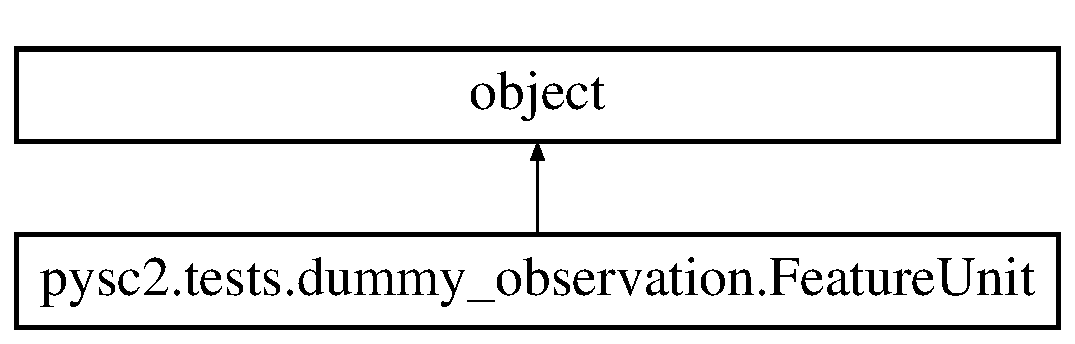
\includegraphics[height=2.000000cm]{classpysc2_1_1tests_1_1dummy__observation_1_1_feature_unit}
\end{center}
\end{figure}
\subsection*{Public Member Functions}
\begin{DoxyCompactItemize}
\item 
def \mbox{\hyperlink{classpysc2_1_1tests_1_1dummy__observation_1_1_feature_unit_a29f045250d5535e17083bbcf76552ce3}{\+\_\+\+\_\+init\+\_\+\+\_\+}} (self, \mbox{\hyperlink{classpysc2_1_1tests_1_1dummy__observation_1_1_feature_unit_a6a9aea1b01b0bef42000625eddd10014}{unit\+\_\+type}}, \mbox{\hyperlink{classpysc2_1_1tests_1_1dummy__observation_1_1_feature_unit_a36f00d3e41958c8cdc28475030b3c8ca}{alliance}}, \mbox{\hyperlink{classpysc2_1_1tests_1_1dummy__observation_1_1_feature_unit_a19974dba093e0d15e69c4d3a791a351e}{owner}}, \mbox{\hyperlink{classpysc2_1_1tests_1_1dummy__observation_1_1_feature_unit_a7c8159cf661d25eb9b130b5209b8b6b2}{pos}}, \mbox{\hyperlink{classpysc2_1_1tests_1_1dummy__observation_1_1_feature_unit_aa77c7afeb2b7b2f1126b45c800447123}{radius}}, \mbox{\hyperlink{classpysc2_1_1tests_1_1dummy__observation_1_1_feature_unit_afa837c7dc75f853f013d5ce4ccac5762}{health}}, \mbox{\hyperlink{classpysc2_1_1tests_1_1dummy__observation_1_1_feature_unit_a33704cb99306a4827b4e4e0ca3398ac8}{health\+\_\+max}}, \mbox{\hyperlink{classpysc2_1_1tests_1_1dummy__observation_1_1_feature_unit_ad9a4ffd45f7af2c034c5463496e12795}{is\+\_\+on\+\_\+screen}}, \mbox{\hyperlink{classpysc2_1_1tests_1_1dummy__observation_1_1_feature_unit_ab551432b8b74984fbf45c160bc3fa216}{shield}}=0, \mbox{\hyperlink{classpysc2_1_1tests_1_1dummy__observation_1_1_feature_unit_a2741bc9f9169631f189e4147ce0ec834}{shield\+\_\+max}}=0, \mbox{\hyperlink{classpysc2_1_1tests_1_1dummy__observation_1_1_feature_unit_ae008fd2fe0f833f0fdeac21a2e572908}{energy}}=0, \mbox{\hyperlink{classpysc2_1_1tests_1_1dummy__observation_1_1_feature_unit_a29a4b2b63ee5fa9f0b19c95615f73c52}{energy\+\_\+max}}=0, \mbox{\hyperlink{classpysc2_1_1tests_1_1dummy__observation_1_1_feature_unit_a31a95dbb0529fd0367f93e6446119107}{cargo\+\_\+space\+\_\+taken}}=0, \mbox{\hyperlink{classpysc2_1_1tests_1_1dummy__observation_1_1_feature_unit_a4b4308329ef1e737110a2677ef70c9c1}{cargo\+\_\+space\+\_\+max}}=0, \mbox{\hyperlink{classpysc2_1_1tests_1_1dummy__observation_1_1_feature_unit_a2bee7ca309a259d0aae8185cec757507}{build\+\_\+progress}}=1.\+0, \mbox{\hyperlink{classpysc2_1_1tests_1_1dummy__observation_1_1_feature_unit_ae4c36a8f2291ab7964e4df4857a4f294}{facing}}=0.\+0, \mbox{\hyperlink{classpysc2_1_1tests_1_1dummy__observation_1_1_feature_unit_afabea5e860553376cf3214b299735e95}{display\+\_\+type}}=raw\+\_\+pb2.\+Visible, \mbox{\hyperlink{classpysc2_1_1tests_1_1dummy__observation_1_1_feature_unit_ab5a1aa4dffa1fe0b4fad110a2d8aca34}{cloak}}=raw\+\_\+pb2.\+Not\+Cloaked, \mbox{\hyperlink{classpysc2_1_1tests_1_1dummy__observation_1_1_feature_unit_a81174e04c9c837ea4236b1c016c1d2b6}{is\+\_\+selected}}=False, \mbox{\hyperlink{classpysc2_1_1tests_1_1dummy__observation_1_1_feature_unit_a2f3c12be40ced78a4c7924c3fc286379}{is\+\_\+blip}}=False, \mbox{\hyperlink{classpysc2_1_1tests_1_1dummy__observation_1_1_feature_unit_a07e6b73d0e672906022fb4f789f18b17}{is\+\_\+powered}}=True, \mbox{\hyperlink{classpysc2_1_1tests_1_1dummy__observation_1_1_feature_unit_a890c00229e399d71a82aeda964cb0b51}{mineral\+\_\+contents}}=0, \mbox{\hyperlink{classpysc2_1_1tests_1_1dummy__observation_1_1_feature_unit_a963db004b55761026732a1214aebf98e}{vespene\+\_\+contents}}=0, \mbox{\hyperlink{classpysc2_1_1tests_1_1dummy__observation_1_1_feature_unit_ac32fb034d2d1b73d71fcb584d0f6da2a}{assigned\+\_\+harvesters}}=0, \mbox{\hyperlink{classpysc2_1_1tests_1_1dummy__observation_1_1_feature_unit_a4519fc0dcdaa63a954bfdb8af3bd8b89}{ideal\+\_\+harvesters}}=0, \mbox{\hyperlink{classpysc2_1_1tests_1_1dummy__observation_1_1_feature_unit_aac10330f3e9ea923e3acff05e87928d9}{weapon\+\_\+cooldown}}=0.\+0)
\item 
def \mbox{\hyperlink{classpysc2_1_1tests_1_1dummy__observation_1_1_feature_unit_a427b9dbadc0902aa5484f00f8a05de60}{as\+\_\+dict}} (self)
\end{DoxyCompactItemize}
\subsection*{Public Attributes}
\begin{DoxyCompactItemize}
\item 
\mbox{\hyperlink{classpysc2_1_1tests_1_1dummy__observation_1_1_feature_unit_a6a9aea1b01b0bef42000625eddd10014}{unit\+\_\+type}}
\item 
\mbox{\hyperlink{classpysc2_1_1tests_1_1dummy__observation_1_1_feature_unit_a36f00d3e41958c8cdc28475030b3c8ca}{alliance}}
\item 
\mbox{\hyperlink{classpysc2_1_1tests_1_1dummy__observation_1_1_feature_unit_a19974dba093e0d15e69c4d3a791a351e}{owner}}
\item 
\mbox{\hyperlink{classpysc2_1_1tests_1_1dummy__observation_1_1_feature_unit_a7c8159cf661d25eb9b130b5209b8b6b2}{pos}}
\item 
\mbox{\hyperlink{classpysc2_1_1tests_1_1dummy__observation_1_1_feature_unit_aa77c7afeb2b7b2f1126b45c800447123}{radius}}
\item 
\mbox{\hyperlink{classpysc2_1_1tests_1_1dummy__observation_1_1_feature_unit_afa837c7dc75f853f013d5ce4ccac5762}{health}}
\item 
\mbox{\hyperlink{classpysc2_1_1tests_1_1dummy__observation_1_1_feature_unit_a33704cb99306a4827b4e4e0ca3398ac8}{health\+\_\+max}}
\item 
\mbox{\hyperlink{classpysc2_1_1tests_1_1dummy__observation_1_1_feature_unit_ad9a4ffd45f7af2c034c5463496e12795}{is\+\_\+on\+\_\+screen}}
\item 
\mbox{\hyperlink{classpysc2_1_1tests_1_1dummy__observation_1_1_feature_unit_ab551432b8b74984fbf45c160bc3fa216}{shield}}
\item 
\mbox{\hyperlink{classpysc2_1_1tests_1_1dummy__observation_1_1_feature_unit_a2741bc9f9169631f189e4147ce0ec834}{shield\+\_\+max}}
\item 
\mbox{\hyperlink{classpysc2_1_1tests_1_1dummy__observation_1_1_feature_unit_ae008fd2fe0f833f0fdeac21a2e572908}{energy}}
\item 
\mbox{\hyperlink{classpysc2_1_1tests_1_1dummy__observation_1_1_feature_unit_a29a4b2b63ee5fa9f0b19c95615f73c52}{energy\+\_\+max}}
\item 
\mbox{\hyperlink{classpysc2_1_1tests_1_1dummy__observation_1_1_feature_unit_a31a95dbb0529fd0367f93e6446119107}{cargo\+\_\+space\+\_\+taken}}
\item 
\mbox{\hyperlink{classpysc2_1_1tests_1_1dummy__observation_1_1_feature_unit_a4b4308329ef1e737110a2677ef70c9c1}{cargo\+\_\+space\+\_\+max}}
\item 
\mbox{\hyperlink{classpysc2_1_1tests_1_1dummy__observation_1_1_feature_unit_a2bee7ca309a259d0aae8185cec757507}{build\+\_\+progress}}
\item 
\mbox{\hyperlink{classpysc2_1_1tests_1_1dummy__observation_1_1_feature_unit_ae4c36a8f2291ab7964e4df4857a4f294}{facing}}
\item 
\mbox{\hyperlink{classpysc2_1_1tests_1_1dummy__observation_1_1_feature_unit_afabea5e860553376cf3214b299735e95}{display\+\_\+type}}
\item 
\mbox{\hyperlink{classpysc2_1_1tests_1_1dummy__observation_1_1_feature_unit_ab5a1aa4dffa1fe0b4fad110a2d8aca34}{cloak}}
\item 
\mbox{\hyperlink{classpysc2_1_1tests_1_1dummy__observation_1_1_feature_unit_a81174e04c9c837ea4236b1c016c1d2b6}{is\+\_\+selected}}
\item 
\mbox{\hyperlink{classpysc2_1_1tests_1_1dummy__observation_1_1_feature_unit_a2f3c12be40ced78a4c7924c3fc286379}{is\+\_\+blip}}
\item 
\mbox{\hyperlink{classpysc2_1_1tests_1_1dummy__observation_1_1_feature_unit_a07e6b73d0e672906022fb4f789f18b17}{is\+\_\+powered}}
\item 
\mbox{\hyperlink{classpysc2_1_1tests_1_1dummy__observation_1_1_feature_unit_a890c00229e399d71a82aeda964cb0b51}{mineral\+\_\+contents}}
\item 
\mbox{\hyperlink{classpysc2_1_1tests_1_1dummy__observation_1_1_feature_unit_a963db004b55761026732a1214aebf98e}{vespene\+\_\+contents}}
\item 
\mbox{\hyperlink{classpysc2_1_1tests_1_1dummy__observation_1_1_feature_unit_ac32fb034d2d1b73d71fcb584d0f6da2a}{assigned\+\_\+harvesters}}
\item 
\mbox{\hyperlink{classpysc2_1_1tests_1_1dummy__observation_1_1_feature_unit_a4519fc0dcdaa63a954bfdb8af3bd8b89}{ideal\+\_\+harvesters}}
\item 
\mbox{\hyperlink{classpysc2_1_1tests_1_1dummy__observation_1_1_feature_unit_aac10330f3e9ea923e3acff05e87928d9}{weapon\+\_\+cooldown}}
\end{DoxyCompactItemize}


\subsection{Detailed Description}
\begin{DoxyVerb}Class to hold feature unit data for the builder.\end{DoxyVerb}
 

\subsection{Constructor \& Destructor Documentation}
\mbox{\Hypertarget{classpysc2_1_1tests_1_1dummy__observation_1_1_feature_unit_a29f045250d5535e17083bbcf76552ce3}\label{classpysc2_1_1tests_1_1dummy__observation_1_1_feature_unit_a29f045250d5535e17083bbcf76552ce3}} 
\index{pysc2\+::tests\+::dummy\+\_\+observation\+::\+Feature\+Unit@{pysc2\+::tests\+::dummy\+\_\+observation\+::\+Feature\+Unit}!\+\_\+\+\_\+init\+\_\+\+\_\+@{\+\_\+\+\_\+init\+\_\+\+\_\+}}
\index{\+\_\+\+\_\+init\+\_\+\+\_\+@{\+\_\+\+\_\+init\+\_\+\+\_\+}!pysc2\+::tests\+::dummy\+\_\+observation\+::\+Feature\+Unit@{pysc2\+::tests\+::dummy\+\_\+observation\+::\+Feature\+Unit}}
\subsubsection{\texorpdfstring{\+\_\+\+\_\+init\+\_\+\+\_\+()}{\_\_init\_\_()}}
{\footnotesize\ttfamily def pysc2.\+tests.\+dummy\+\_\+observation.\+Feature\+Unit.\+\_\+\+\_\+init\+\_\+\+\_\+ (\begin{DoxyParamCaption}\item[{}]{self,  }\item[{}]{unit\+\_\+type,  }\item[{}]{alliance,  }\item[{}]{owner,  }\item[{}]{pos,  }\item[{}]{radius,  }\item[{}]{health,  }\item[{}]{health\+\_\+max,  }\item[{}]{is\+\_\+on\+\_\+screen,  }\item[{}]{shield = {\ttfamily 0},  }\item[{}]{shield\+\_\+max = {\ttfamily 0},  }\item[{}]{energy = {\ttfamily 0},  }\item[{}]{energy\+\_\+max = {\ttfamily 0},  }\item[{}]{cargo\+\_\+space\+\_\+taken = {\ttfamily 0},  }\item[{}]{cargo\+\_\+space\+\_\+max = {\ttfamily 0},  }\item[{}]{build\+\_\+progress = {\ttfamily 1.0},  }\item[{}]{facing = {\ttfamily 0.0},  }\item[{}]{display\+\_\+type = {\ttfamily raw\+\_\+pb2.Visible},  }\item[{}]{cloak = {\ttfamily raw\+\_\+pb2.NotCloaked},  }\item[{}]{is\+\_\+selected = {\ttfamily False},  }\item[{}]{is\+\_\+blip = {\ttfamily False},  }\item[{}]{is\+\_\+powered = {\ttfamily True},  }\item[{}]{mineral\+\_\+contents = {\ttfamily 0},  }\item[{}]{vespene\+\_\+contents = {\ttfamily 0},  }\item[{}]{assigned\+\_\+harvesters = {\ttfamily 0},  }\item[{}]{ideal\+\_\+harvesters = {\ttfamily 0},  }\item[{}]{weapon\+\_\+cooldown = {\ttfamily 0.0} }\end{DoxyParamCaption})}



\subsection{Member Function Documentation}
\mbox{\Hypertarget{classpysc2_1_1tests_1_1dummy__observation_1_1_feature_unit_a427b9dbadc0902aa5484f00f8a05de60}\label{classpysc2_1_1tests_1_1dummy__observation_1_1_feature_unit_a427b9dbadc0902aa5484f00f8a05de60}} 
\index{pysc2\+::tests\+::dummy\+\_\+observation\+::\+Feature\+Unit@{pysc2\+::tests\+::dummy\+\_\+observation\+::\+Feature\+Unit}!as\+\_\+dict@{as\+\_\+dict}}
\index{as\+\_\+dict@{as\+\_\+dict}!pysc2\+::tests\+::dummy\+\_\+observation\+::\+Feature\+Unit@{pysc2\+::tests\+::dummy\+\_\+observation\+::\+Feature\+Unit}}
\subsubsection{\texorpdfstring{as\+\_\+dict()}{as\_dict()}}
{\footnotesize\ttfamily def pysc2.\+tests.\+dummy\+\_\+observation.\+Feature\+Unit.\+as\+\_\+dict (\begin{DoxyParamCaption}\item[{}]{self }\end{DoxyParamCaption})}



\subsection{Member Data Documentation}
\mbox{\Hypertarget{classpysc2_1_1tests_1_1dummy__observation_1_1_feature_unit_a36f00d3e41958c8cdc28475030b3c8ca}\label{classpysc2_1_1tests_1_1dummy__observation_1_1_feature_unit_a36f00d3e41958c8cdc28475030b3c8ca}} 
\index{pysc2\+::tests\+::dummy\+\_\+observation\+::\+Feature\+Unit@{pysc2\+::tests\+::dummy\+\_\+observation\+::\+Feature\+Unit}!alliance@{alliance}}
\index{alliance@{alliance}!pysc2\+::tests\+::dummy\+\_\+observation\+::\+Feature\+Unit@{pysc2\+::tests\+::dummy\+\_\+observation\+::\+Feature\+Unit}}
\subsubsection{\texorpdfstring{alliance}{alliance}}
{\footnotesize\ttfamily pysc2.\+tests.\+dummy\+\_\+observation.\+Feature\+Unit.\+alliance}

\mbox{\Hypertarget{classpysc2_1_1tests_1_1dummy__observation_1_1_feature_unit_ac32fb034d2d1b73d71fcb584d0f6da2a}\label{classpysc2_1_1tests_1_1dummy__observation_1_1_feature_unit_ac32fb034d2d1b73d71fcb584d0f6da2a}} 
\index{pysc2\+::tests\+::dummy\+\_\+observation\+::\+Feature\+Unit@{pysc2\+::tests\+::dummy\+\_\+observation\+::\+Feature\+Unit}!assigned\+\_\+harvesters@{assigned\+\_\+harvesters}}
\index{assigned\+\_\+harvesters@{assigned\+\_\+harvesters}!pysc2\+::tests\+::dummy\+\_\+observation\+::\+Feature\+Unit@{pysc2\+::tests\+::dummy\+\_\+observation\+::\+Feature\+Unit}}
\subsubsection{\texorpdfstring{assigned\+\_\+harvesters}{assigned\_harvesters}}
{\footnotesize\ttfamily pysc2.\+tests.\+dummy\+\_\+observation.\+Feature\+Unit.\+assigned\+\_\+harvesters}

\mbox{\Hypertarget{classpysc2_1_1tests_1_1dummy__observation_1_1_feature_unit_a2bee7ca309a259d0aae8185cec757507}\label{classpysc2_1_1tests_1_1dummy__observation_1_1_feature_unit_a2bee7ca309a259d0aae8185cec757507}} 
\index{pysc2\+::tests\+::dummy\+\_\+observation\+::\+Feature\+Unit@{pysc2\+::tests\+::dummy\+\_\+observation\+::\+Feature\+Unit}!build\+\_\+progress@{build\+\_\+progress}}
\index{build\+\_\+progress@{build\+\_\+progress}!pysc2\+::tests\+::dummy\+\_\+observation\+::\+Feature\+Unit@{pysc2\+::tests\+::dummy\+\_\+observation\+::\+Feature\+Unit}}
\subsubsection{\texorpdfstring{build\+\_\+progress}{build\_progress}}
{\footnotesize\ttfamily pysc2.\+tests.\+dummy\+\_\+observation.\+Feature\+Unit.\+build\+\_\+progress}

\mbox{\Hypertarget{classpysc2_1_1tests_1_1dummy__observation_1_1_feature_unit_a4b4308329ef1e737110a2677ef70c9c1}\label{classpysc2_1_1tests_1_1dummy__observation_1_1_feature_unit_a4b4308329ef1e737110a2677ef70c9c1}} 
\index{pysc2\+::tests\+::dummy\+\_\+observation\+::\+Feature\+Unit@{pysc2\+::tests\+::dummy\+\_\+observation\+::\+Feature\+Unit}!cargo\+\_\+space\+\_\+max@{cargo\+\_\+space\+\_\+max}}
\index{cargo\+\_\+space\+\_\+max@{cargo\+\_\+space\+\_\+max}!pysc2\+::tests\+::dummy\+\_\+observation\+::\+Feature\+Unit@{pysc2\+::tests\+::dummy\+\_\+observation\+::\+Feature\+Unit}}
\subsubsection{\texorpdfstring{cargo\+\_\+space\+\_\+max}{cargo\_space\_max}}
{\footnotesize\ttfamily pysc2.\+tests.\+dummy\+\_\+observation.\+Feature\+Unit.\+cargo\+\_\+space\+\_\+max}

\mbox{\Hypertarget{classpysc2_1_1tests_1_1dummy__observation_1_1_feature_unit_a31a95dbb0529fd0367f93e6446119107}\label{classpysc2_1_1tests_1_1dummy__observation_1_1_feature_unit_a31a95dbb0529fd0367f93e6446119107}} 
\index{pysc2\+::tests\+::dummy\+\_\+observation\+::\+Feature\+Unit@{pysc2\+::tests\+::dummy\+\_\+observation\+::\+Feature\+Unit}!cargo\+\_\+space\+\_\+taken@{cargo\+\_\+space\+\_\+taken}}
\index{cargo\+\_\+space\+\_\+taken@{cargo\+\_\+space\+\_\+taken}!pysc2\+::tests\+::dummy\+\_\+observation\+::\+Feature\+Unit@{pysc2\+::tests\+::dummy\+\_\+observation\+::\+Feature\+Unit}}
\subsubsection{\texorpdfstring{cargo\+\_\+space\+\_\+taken}{cargo\_space\_taken}}
{\footnotesize\ttfamily pysc2.\+tests.\+dummy\+\_\+observation.\+Feature\+Unit.\+cargo\+\_\+space\+\_\+taken}

\mbox{\Hypertarget{classpysc2_1_1tests_1_1dummy__observation_1_1_feature_unit_ab5a1aa4dffa1fe0b4fad110a2d8aca34}\label{classpysc2_1_1tests_1_1dummy__observation_1_1_feature_unit_ab5a1aa4dffa1fe0b4fad110a2d8aca34}} 
\index{pysc2\+::tests\+::dummy\+\_\+observation\+::\+Feature\+Unit@{pysc2\+::tests\+::dummy\+\_\+observation\+::\+Feature\+Unit}!cloak@{cloak}}
\index{cloak@{cloak}!pysc2\+::tests\+::dummy\+\_\+observation\+::\+Feature\+Unit@{pysc2\+::tests\+::dummy\+\_\+observation\+::\+Feature\+Unit}}
\subsubsection{\texorpdfstring{cloak}{cloak}}
{\footnotesize\ttfamily pysc2.\+tests.\+dummy\+\_\+observation.\+Feature\+Unit.\+cloak}

\mbox{\Hypertarget{classpysc2_1_1tests_1_1dummy__observation_1_1_feature_unit_afabea5e860553376cf3214b299735e95}\label{classpysc2_1_1tests_1_1dummy__observation_1_1_feature_unit_afabea5e860553376cf3214b299735e95}} 
\index{pysc2\+::tests\+::dummy\+\_\+observation\+::\+Feature\+Unit@{pysc2\+::tests\+::dummy\+\_\+observation\+::\+Feature\+Unit}!display\+\_\+type@{display\+\_\+type}}
\index{display\+\_\+type@{display\+\_\+type}!pysc2\+::tests\+::dummy\+\_\+observation\+::\+Feature\+Unit@{pysc2\+::tests\+::dummy\+\_\+observation\+::\+Feature\+Unit}}
\subsubsection{\texorpdfstring{display\+\_\+type}{display\_type}}
{\footnotesize\ttfamily pysc2.\+tests.\+dummy\+\_\+observation.\+Feature\+Unit.\+display\+\_\+type}

\mbox{\Hypertarget{classpysc2_1_1tests_1_1dummy__observation_1_1_feature_unit_ae008fd2fe0f833f0fdeac21a2e572908}\label{classpysc2_1_1tests_1_1dummy__observation_1_1_feature_unit_ae008fd2fe0f833f0fdeac21a2e572908}} 
\index{pysc2\+::tests\+::dummy\+\_\+observation\+::\+Feature\+Unit@{pysc2\+::tests\+::dummy\+\_\+observation\+::\+Feature\+Unit}!energy@{energy}}
\index{energy@{energy}!pysc2\+::tests\+::dummy\+\_\+observation\+::\+Feature\+Unit@{pysc2\+::tests\+::dummy\+\_\+observation\+::\+Feature\+Unit}}
\subsubsection{\texorpdfstring{energy}{energy}}
{\footnotesize\ttfamily pysc2.\+tests.\+dummy\+\_\+observation.\+Feature\+Unit.\+energy}

\mbox{\Hypertarget{classpysc2_1_1tests_1_1dummy__observation_1_1_feature_unit_a29a4b2b63ee5fa9f0b19c95615f73c52}\label{classpysc2_1_1tests_1_1dummy__observation_1_1_feature_unit_a29a4b2b63ee5fa9f0b19c95615f73c52}} 
\index{pysc2\+::tests\+::dummy\+\_\+observation\+::\+Feature\+Unit@{pysc2\+::tests\+::dummy\+\_\+observation\+::\+Feature\+Unit}!energy\+\_\+max@{energy\+\_\+max}}
\index{energy\+\_\+max@{energy\+\_\+max}!pysc2\+::tests\+::dummy\+\_\+observation\+::\+Feature\+Unit@{pysc2\+::tests\+::dummy\+\_\+observation\+::\+Feature\+Unit}}
\subsubsection{\texorpdfstring{energy\+\_\+max}{energy\_max}}
{\footnotesize\ttfamily pysc2.\+tests.\+dummy\+\_\+observation.\+Feature\+Unit.\+energy\+\_\+max}

\mbox{\Hypertarget{classpysc2_1_1tests_1_1dummy__observation_1_1_feature_unit_ae4c36a8f2291ab7964e4df4857a4f294}\label{classpysc2_1_1tests_1_1dummy__observation_1_1_feature_unit_ae4c36a8f2291ab7964e4df4857a4f294}} 
\index{pysc2\+::tests\+::dummy\+\_\+observation\+::\+Feature\+Unit@{pysc2\+::tests\+::dummy\+\_\+observation\+::\+Feature\+Unit}!facing@{facing}}
\index{facing@{facing}!pysc2\+::tests\+::dummy\+\_\+observation\+::\+Feature\+Unit@{pysc2\+::tests\+::dummy\+\_\+observation\+::\+Feature\+Unit}}
\subsubsection{\texorpdfstring{facing}{facing}}
{\footnotesize\ttfamily pysc2.\+tests.\+dummy\+\_\+observation.\+Feature\+Unit.\+facing}

\mbox{\Hypertarget{classpysc2_1_1tests_1_1dummy__observation_1_1_feature_unit_afa837c7dc75f853f013d5ce4ccac5762}\label{classpysc2_1_1tests_1_1dummy__observation_1_1_feature_unit_afa837c7dc75f853f013d5ce4ccac5762}} 
\index{pysc2\+::tests\+::dummy\+\_\+observation\+::\+Feature\+Unit@{pysc2\+::tests\+::dummy\+\_\+observation\+::\+Feature\+Unit}!health@{health}}
\index{health@{health}!pysc2\+::tests\+::dummy\+\_\+observation\+::\+Feature\+Unit@{pysc2\+::tests\+::dummy\+\_\+observation\+::\+Feature\+Unit}}
\subsubsection{\texorpdfstring{health}{health}}
{\footnotesize\ttfamily pysc2.\+tests.\+dummy\+\_\+observation.\+Feature\+Unit.\+health}

\mbox{\Hypertarget{classpysc2_1_1tests_1_1dummy__observation_1_1_feature_unit_a33704cb99306a4827b4e4e0ca3398ac8}\label{classpysc2_1_1tests_1_1dummy__observation_1_1_feature_unit_a33704cb99306a4827b4e4e0ca3398ac8}} 
\index{pysc2\+::tests\+::dummy\+\_\+observation\+::\+Feature\+Unit@{pysc2\+::tests\+::dummy\+\_\+observation\+::\+Feature\+Unit}!health\+\_\+max@{health\+\_\+max}}
\index{health\+\_\+max@{health\+\_\+max}!pysc2\+::tests\+::dummy\+\_\+observation\+::\+Feature\+Unit@{pysc2\+::tests\+::dummy\+\_\+observation\+::\+Feature\+Unit}}
\subsubsection{\texorpdfstring{health\+\_\+max}{health\_max}}
{\footnotesize\ttfamily pysc2.\+tests.\+dummy\+\_\+observation.\+Feature\+Unit.\+health\+\_\+max}

\mbox{\Hypertarget{classpysc2_1_1tests_1_1dummy__observation_1_1_feature_unit_a4519fc0dcdaa63a954bfdb8af3bd8b89}\label{classpysc2_1_1tests_1_1dummy__observation_1_1_feature_unit_a4519fc0dcdaa63a954bfdb8af3bd8b89}} 
\index{pysc2\+::tests\+::dummy\+\_\+observation\+::\+Feature\+Unit@{pysc2\+::tests\+::dummy\+\_\+observation\+::\+Feature\+Unit}!ideal\+\_\+harvesters@{ideal\+\_\+harvesters}}
\index{ideal\+\_\+harvesters@{ideal\+\_\+harvesters}!pysc2\+::tests\+::dummy\+\_\+observation\+::\+Feature\+Unit@{pysc2\+::tests\+::dummy\+\_\+observation\+::\+Feature\+Unit}}
\subsubsection{\texorpdfstring{ideal\+\_\+harvesters}{ideal\_harvesters}}
{\footnotesize\ttfamily pysc2.\+tests.\+dummy\+\_\+observation.\+Feature\+Unit.\+ideal\+\_\+harvesters}

\mbox{\Hypertarget{classpysc2_1_1tests_1_1dummy__observation_1_1_feature_unit_a2f3c12be40ced78a4c7924c3fc286379}\label{classpysc2_1_1tests_1_1dummy__observation_1_1_feature_unit_a2f3c12be40ced78a4c7924c3fc286379}} 
\index{pysc2\+::tests\+::dummy\+\_\+observation\+::\+Feature\+Unit@{pysc2\+::tests\+::dummy\+\_\+observation\+::\+Feature\+Unit}!is\+\_\+blip@{is\+\_\+blip}}
\index{is\+\_\+blip@{is\+\_\+blip}!pysc2\+::tests\+::dummy\+\_\+observation\+::\+Feature\+Unit@{pysc2\+::tests\+::dummy\+\_\+observation\+::\+Feature\+Unit}}
\subsubsection{\texorpdfstring{is\+\_\+blip}{is\_blip}}
{\footnotesize\ttfamily pysc2.\+tests.\+dummy\+\_\+observation.\+Feature\+Unit.\+is\+\_\+blip}

\mbox{\Hypertarget{classpysc2_1_1tests_1_1dummy__observation_1_1_feature_unit_ad9a4ffd45f7af2c034c5463496e12795}\label{classpysc2_1_1tests_1_1dummy__observation_1_1_feature_unit_ad9a4ffd45f7af2c034c5463496e12795}} 
\index{pysc2\+::tests\+::dummy\+\_\+observation\+::\+Feature\+Unit@{pysc2\+::tests\+::dummy\+\_\+observation\+::\+Feature\+Unit}!is\+\_\+on\+\_\+screen@{is\+\_\+on\+\_\+screen}}
\index{is\+\_\+on\+\_\+screen@{is\+\_\+on\+\_\+screen}!pysc2\+::tests\+::dummy\+\_\+observation\+::\+Feature\+Unit@{pysc2\+::tests\+::dummy\+\_\+observation\+::\+Feature\+Unit}}
\subsubsection{\texorpdfstring{is\+\_\+on\+\_\+screen}{is\_on\_screen}}
{\footnotesize\ttfamily pysc2.\+tests.\+dummy\+\_\+observation.\+Feature\+Unit.\+is\+\_\+on\+\_\+screen}

\mbox{\Hypertarget{classpysc2_1_1tests_1_1dummy__observation_1_1_feature_unit_a07e6b73d0e672906022fb4f789f18b17}\label{classpysc2_1_1tests_1_1dummy__observation_1_1_feature_unit_a07e6b73d0e672906022fb4f789f18b17}} 
\index{pysc2\+::tests\+::dummy\+\_\+observation\+::\+Feature\+Unit@{pysc2\+::tests\+::dummy\+\_\+observation\+::\+Feature\+Unit}!is\+\_\+powered@{is\+\_\+powered}}
\index{is\+\_\+powered@{is\+\_\+powered}!pysc2\+::tests\+::dummy\+\_\+observation\+::\+Feature\+Unit@{pysc2\+::tests\+::dummy\+\_\+observation\+::\+Feature\+Unit}}
\subsubsection{\texorpdfstring{is\+\_\+powered}{is\_powered}}
{\footnotesize\ttfamily pysc2.\+tests.\+dummy\+\_\+observation.\+Feature\+Unit.\+is\+\_\+powered}

\mbox{\Hypertarget{classpysc2_1_1tests_1_1dummy__observation_1_1_feature_unit_a81174e04c9c837ea4236b1c016c1d2b6}\label{classpysc2_1_1tests_1_1dummy__observation_1_1_feature_unit_a81174e04c9c837ea4236b1c016c1d2b6}} 
\index{pysc2\+::tests\+::dummy\+\_\+observation\+::\+Feature\+Unit@{pysc2\+::tests\+::dummy\+\_\+observation\+::\+Feature\+Unit}!is\+\_\+selected@{is\+\_\+selected}}
\index{is\+\_\+selected@{is\+\_\+selected}!pysc2\+::tests\+::dummy\+\_\+observation\+::\+Feature\+Unit@{pysc2\+::tests\+::dummy\+\_\+observation\+::\+Feature\+Unit}}
\subsubsection{\texorpdfstring{is\+\_\+selected}{is\_selected}}
{\footnotesize\ttfamily pysc2.\+tests.\+dummy\+\_\+observation.\+Feature\+Unit.\+is\+\_\+selected}

\mbox{\Hypertarget{classpysc2_1_1tests_1_1dummy__observation_1_1_feature_unit_a890c00229e399d71a82aeda964cb0b51}\label{classpysc2_1_1tests_1_1dummy__observation_1_1_feature_unit_a890c00229e399d71a82aeda964cb0b51}} 
\index{pysc2\+::tests\+::dummy\+\_\+observation\+::\+Feature\+Unit@{pysc2\+::tests\+::dummy\+\_\+observation\+::\+Feature\+Unit}!mineral\+\_\+contents@{mineral\+\_\+contents}}
\index{mineral\+\_\+contents@{mineral\+\_\+contents}!pysc2\+::tests\+::dummy\+\_\+observation\+::\+Feature\+Unit@{pysc2\+::tests\+::dummy\+\_\+observation\+::\+Feature\+Unit}}
\subsubsection{\texorpdfstring{mineral\+\_\+contents}{mineral\_contents}}
{\footnotesize\ttfamily pysc2.\+tests.\+dummy\+\_\+observation.\+Feature\+Unit.\+mineral\+\_\+contents}

\mbox{\Hypertarget{classpysc2_1_1tests_1_1dummy__observation_1_1_feature_unit_a19974dba093e0d15e69c4d3a791a351e}\label{classpysc2_1_1tests_1_1dummy__observation_1_1_feature_unit_a19974dba093e0d15e69c4d3a791a351e}} 
\index{pysc2\+::tests\+::dummy\+\_\+observation\+::\+Feature\+Unit@{pysc2\+::tests\+::dummy\+\_\+observation\+::\+Feature\+Unit}!owner@{owner}}
\index{owner@{owner}!pysc2\+::tests\+::dummy\+\_\+observation\+::\+Feature\+Unit@{pysc2\+::tests\+::dummy\+\_\+observation\+::\+Feature\+Unit}}
\subsubsection{\texorpdfstring{owner}{owner}}
{\footnotesize\ttfamily pysc2.\+tests.\+dummy\+\_\+observation.\+Feature\+Unit.\+owner}

\mbox{\Hypertarget{classpysc2_1_1tests_1_1dummy__observation_1_1_feature_unit_a7c8159cf661d25eb9b130b5209b8b6b2}\label{classpysc2_1_1tests_1_1dummy__observation_1_1_feature_unit_a7c8159cf661d25eb9b130b5209b8b6b2}} 
\index{pysc2\+::tests\+::dummy\+\_\+observation\+::\+Feature\+Unit@{pysc2\+::tests\+::dummy\+\_\+observation\+::\+Feature\+Unit}!pos@{pos}}
\index{pos@{pos}!pysc2\+::tests\+::dummy\+\_\+observation\+::\+Feature\+Unit@{pysc2\+::tests\+::dummy\+\_\+observation\+::\+Feature\+Unit}}
\subsubsection{\texorpdfstring{pos}{pos}}
{\footnotesize\ttfamily pysc2.\+tests.\+dummy\+\_\+observation.\+Feature\+Unit.\+pos}

\mbox{\Hypertarget{classpysc2_1_1tests_1_1dummy__observation_1_1_feature_unit_aa77c7afeb2b7b2f1126b45c800447123}\label{classpysc2_1_1tests_1_1dummy__observation_1_1_feature_unit_aa77c7afeb2b7b2f1126b45c800447123}} 
\index{pysc2\+::tests\+::dummy\+\_\+observation\+::\+Feature\+Unit@{pysc2\+::tests\+::dummy\+\_\+observation\+::\+Feature\+Unit}!radius@{radius}}
\index{radius@{radius}!pysc2\+::tests\+::dummy\+\_\+observation\+::\+Feature\+Unit@{pysc2\+::tests\+::dummy\+\_\+observation\+::\+Feature\+Unit}}
\subsubsection{\texorpdfstring{radius}{radius}}
{\footnotesize\ttfamily pysc2.\+tests.\+dummy\+\_\+observation.\+Feature\+Unit.\+radius}

\mbox{\Hypertarget{classpysc2_1_1tests_1_1dummy__observation_1_1_feature_unit_ab551432b8b74984fbf45c160bc3fa216}\label{classpysc2_1_1tests_1_1dummy__observation_1_1_feature_unit_ab551432b8b74984fbf45c160bc3fa216}} 
\index{pysc2\+::tests\+::dummy\+\_\+observation\+::\+Feature\+Unit@{pysc2\+::tests\+::dummy\+\_\+observation\+::\+Feature\+Unit}!shield@{shield}}
\index{shield@{shield}!pysc2\+::tests\+::dummy\+\_\+observation\+::\+Feature\+Unit@{pysc2\+::tests\+::dummy\+\_\+observation\+::\+Feature\+Unit}}
\subsubsection{\texorpdfstring{shield}{shield}}
{\footnotesize\ttfamily pysc2.\+tests.\+dummy\+\_\+observation.\+Feature\+Unit.\+shield}

\mbox{\Hypertarget{classpysc2_1_1tests_1_1dummy__observation_1_1_feature_unit_a2741bc9f9169631f189e4147ce0ec834}\label{classpysc2_1_1tests_1_1dummy__observation_1_1_feature_unit_a2741bc9f9169631f189e4147ce0ec834}} 
\index{pysc2\+::tests\+::dummy\+\_\+observation\+::\+Feature\+Unit@{pysc2\+::tests\+::dummy\+\_\+observation\+::\+Feature\+Unit}!shield\+\_\+max@{shield\+\_\+max}}
\index{shield\+\_\+max@{shield\+\_\+max}!pysc2\+::tests\+::dummy\+\_\+observation\+::\+Feature\+Unit@{pysc2\+::tests\+::dummy\+\_\+observation\+::\+Feature\+Unit}}
\subsubsection{\texorpdfstring{shield\+\_\+max}{shield\_max}}
{\footnotesize\ttfamily pysc2.\+tests.\+dummy\+\_\+observation.\+Feature\+Unit.\+shield\+\_\+max}

\mbox{\Hypertarget{classpysc2_1_1tests_1_1dummy__observation_1_1_feature_unit_a6a9aea1b01b0bef42000625eddd10014}\label{classpysc2_1_1tests_1_1dummy__observation_1_1_feature_unit_a6a9aea1b01b0bef42000625eddd10014}} 
\index{pysc2\+::tests\+::dummy\+\_\+observation\+::\+Feature\+Unit@{pysc2\+::tests\+::dummy\+\_\+observation\+::\+Feature\+Unit}!unit\+\_\+type@{unit\+\_\+type}}
\index{unit\+\_\+type@{unit\+\_\+type}!pysc2\+::tests\+::dummy\+\_\+observation\+::\+Feature\+Unit@{pysc2\+::tests\+::dummy\+\_\+observation\+::\+Feature\+Unit}}
\subsubsection{\texorpdfstring{unit\+\_\+type}{unit\_type}}
{\footnotesize\ttfamily pysc2.\+tests.\+dummy\+\_\+observation.\+Feature\+Unit.\+unit\+\_\+type}

\mbox{\Hypertarget{classpysc2_1_1tests_1_1dummy__observation_1_1_feature_unit_a963db004b55761026732a1214aebf98e}\label{classpysc2_1_1tests_1_1dummy__observation_1_1_feature_unit_a963db004b55761026732a1214aebf98e}} 
\index{pysc2\+::tests\+::dummy\+\_\+observation\+::\+Feature\+Unit@{pysc2\+::tests\+::dummy\+\_\+observation\+::\+Feature\+Unit}!vespene\+\_\+contents@{vespene\+\_\+contents}}
\index{vespene\+\_\+contents@{vespene\+\_\+contents}!pysc2\+::tests\+::dummy\+\_\+observation\+::\+Feature\+Unit@{pysc2\+::tests\+::dummy\+\_\+observation\+::\+Feature\+Unit}}
\subsubsection{\texorpdfstring{vespene\+\_\+contents}{vespene\_contents}}
{\footnotesize\ttfamily pysc2.\+tests.\+dummy\+\_\+observation.\+Feature\+Unit.\+vespene\+\_\+contents}

\mbox{\Hypertarget{classpysc2_1_1tests_1_1dummy__observation_1_1_feature_unit_aac10330f3e9ea923e3acff05e87928d9}\label{classpysc2_1_1tests_1_1dummy__observation_1_1_feature_unit_aac10330f3e9ea923e3acff05e87928d9}} 
\index{pysc2\+::tests\+::dummy\+\_\+observation\+::\+Feature\+Unit@{pysc2\+::tests\+::dummy\+\_\+observation\+::\+Feature\+Unit}!weapon\+\_\+cooldown@{weapon\+\_\+cooldown}}
\index{weapon\+\_\+cooldown@{weapon\+\_\+cooldown}!pysc2\+::tests\+::dummy\+\_\+observation\+::\+Feature\+Unit@{pysc2\+::tests\+::dummy\+\_\+observation\+::\+Feature\+Unit}}
\subsubsection{\texorpdfstring{weapon\+\_\+cooldown}{weapon\_cooldown}}
{\footnotesize\ttfamily pysc2.\+tests.\+dummy\+\_\+observation.\+Feature\+Unit.\+weapon\+\_\+cooldown}



The documentation for this class was generated from the following file\+:\begin{DoxyCompactItemize}
\item 
tests/\mbox{\hyperlink{dummy__observation_8py}{dummy\+\_\+observation.\+py}}\end{DoxyCompactItemize}

\hypertarget{classpysc2_1_1lib_1_1actions_1_1_function}{}\section{pysc2.\+lib.\+actions.\+Function Class Reference}
\label{classpysc2_1_1lib_1_1actions_1_1_function}\index{pysc2.\+lib.\+actions.\+Function@{pysc2.\+lib.\+actions.\+Function}}
Inheritance diagram for pysc2.\+lib.\+actions.\+Function\+:\begin{figure}[H]
\begin{center}
\leavevmode
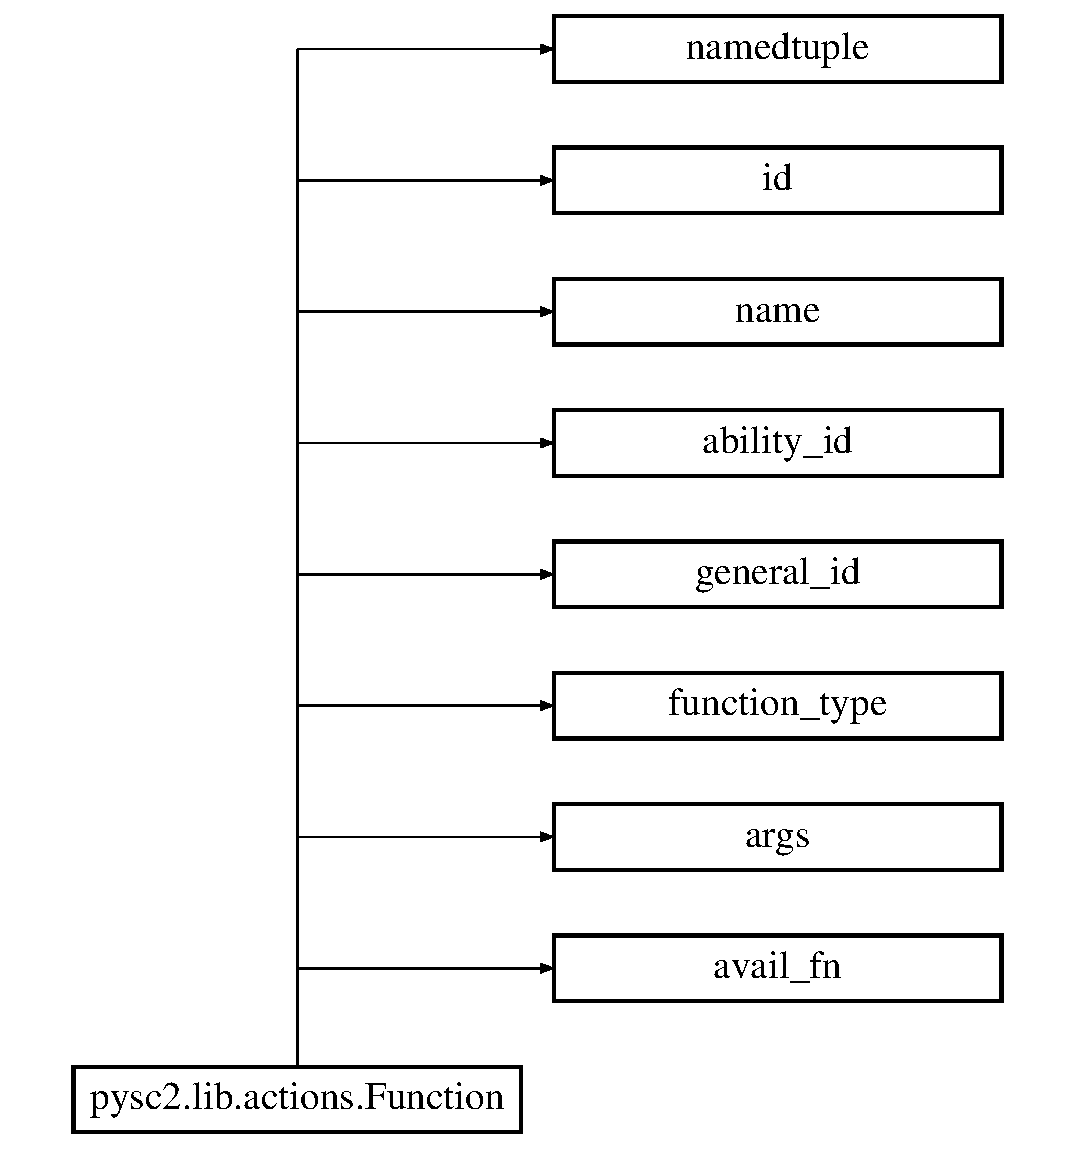
\includegraphics[height=9.000000cm]{classpysc2_1_1lib_1_1actions_1_1_function}
\end{center}
\end{figure}
\subsection*{Public Member Functions}
\begin{DoxyCompactItemize}
\item 
def \mbox{\hyperlink{classpysc2_1_1lib_1_1actions_1_1_function_a2c4bb777e80bd4cdeaa012e85f85b4be}{ui\+\_\+func}} (cls, id\+\_\+, name, function\+\_\+type, avail\+\_\+fn=\mbox{\hyperlink{namespacepysc2_1_1lib_1_1actions_ae1dc5f547908d78c7367d3c734b29a59}{always}})
\item 
def \mbox{\hyperlink{classpysc2_1_1lib_1_1actions_1_1_function_afa5332609b8f6e69057a0035add0a480}{ability}} (cls, id\+\_\+, name, function\+\_\+type, ability\+\_\+id, general\+\_\+id=0)
\item 
def \mbox{\hyperlink{classpysc2_1_1lib_1_1actions_1_1_function_a640d6d3480535d03e1b11cd4314ab221}{spec}} (cls, id\+\_\+, name, args)
\item 
def \mbox{\hyperlink{classpysc2_1_1lib_1_1actions_1_1_function_a31e8c8775ce3b7d55671b1494502aca7}{\+\_\+\+\_\+hash\+\_\+\+\_\+}} (self)
\item 
def \mbox{\hyperlink{classpysc2_1_1lib_1_1actions_1_1_function_a693e39932ef61edb079e977f8636626e}{\+\_\+\+\_\+str\+\_\+\+\_\+}} (self)
\item 
def \mbox{\hyperlink{classpysc2_1_1lib_1_1actions_1_1_function_a82d083b88887fb4c9fa6dd99a399cedc}{\+\_\+\+\_\+call\+\_\+\+\_\+}} (self, args)
\item 
def \mbox{\hyperlink{classpysc2_1_1lib_1_1actions_1_1_function_a98ad5ff5cc2cbd2656c25dbf0d60c8a4}{str}} (self, space=False)
\end{DoxyCompactItemize}


\subsection{Detailed Description}
\begin{DoxyVerb}Represents a function action.

Attributes:
  id: The function id, which is what the agent will use.
  name: The name of the function. Should be unique.
  ability_id: The ability id to pass to sc2.
  general_id: 0 for normal abilities, and the ability_id of another ability if
      it can be represented by a more general action.
  function_type: One of the functions in FUNCTION_TYPES for how to construct
      the sc2 action proto out of python types.
  args: A list of the types of args passed to function_type.
  avail_fn: For non-abilities, this function returns whether the function is
      valid.
\end{DoxyVerb}
 

\subsection{Member Function Documentation}
\mbox{\Hypertarget{classpysc2_1_1lib_1_1actions_1_1_function_a82d083b88887fb4c9fa6dd99a399cedc}\label{classpysc2_1_1lib_1_1actions_1_1_function_a82d083b88887fb4c9fa6dd99a399cedc}} 
\index{pysc2\+::lib\+::actions\+::\+Function@{pysc2\+::lib\+::actions\+::\+Function}!\+\_\+\+\_\+call\+\_\+\+\_\+@{\+\_\+\+\_\+call\+\_\+\+\_\+}}
\index{\+\_\+\+\_\+call\+\_\+\+\_\+@{\+\_\+\+\_\+call\+\_\+\+\_\+}!pysc2\+::lib\+::actions\+::\+Function@{pysc2\+::lib\+::actions\+::\+Function}}
\subsubsection{\texorpdfstring{\+\_\+\+\_\+call\+\_\+\+\_\+()}{\_\_call\_\_()}}
{\footnotesize\ttfamily def pysc2.\+lib.\+actions.\+Function.\+\_\+\+\_\+call\+\_\+\+\_\+ (\begin{DoxyParamCaption}\item[{}]{self,  }\item[{}]{args }\end{DoxyParamCaption})}

\begin{DoxyVerb}A convenient way to create a FunctionCall from this Function.\end{DoxyVerb}
 \mbox{\Hypertarget{classpysc2_1_1lib_1_1actions_1_1_function_a31e8c8775ce3b7d55671b1494502aca7}\label{classpysc2_1_1lib_1_1actions_1_1_function_a31e8c8775ce3b7d55671b1494502aca7}} 
\index{pysc2\+::lib\+::actions\+::\+Function@{pysc2\+::lib\+::actions\+::\+Function}!\+\_\+\+\_\+hash\+\_\+\+\_\+@{\+\_\+\+\_\+hash\+\_\+\+\_\+}}
\index{\+\_\+\+\_\+hash\+\_\+\+\_\+@{\+\_\+\+\_\+hash\+\_\+\+\_\+}!pysc2\+::lib\+::actions\+::\+Function@{pysc2\+::lib\+::actions\+::\+Function}}
\subsubsection{\texorpdfstring{\+\_\+\+\_\+hash\+\_\+\+\_\+()}{\_\_hash\_\_()}}
{\footnotesize\ttfamily def pysc2.\+lib.\+actions.\+Function.\+\_\+\+\_\+hash\+\_\+\+\_\+ (\begin{DoxyParamCaption}\item[{}]{self }\end{DoxyParamCaption})}

\mbox{\Hypertarget{classpysc2_1_1lib_1_1actions_1_1_function_a693e39932ef61edb079e977f8636626e}\label{classpysc2_1_1lib_1_1actions_1_1_function_a693e39932ef61edb079e977f8636626e}} 
\index{pysc2\+::lib\+::actions\+::\+Function@{pysc2\+::lib\+::actions\+::\+Function}!\+\_\+\+\_\+str\+\_\+\+\_\+@{\+\_\+\+\_\+str\+\_\+\+\_\+}}
\index{\+\_\+\+\_\+str\+\_\+\+\_\+@{\+\_\+\+\_\+str\+\_\+\+\_\+}!pysc2\+::lib\+::actions\+::\+Function@{pysc2\+::lib\+::actions\+::\+Function}}
\subsubsection{\texorpdfstring{\+\_\+\+\_\+str\+\_\+\+\_\+()}{\_\_str\_\_()}}
{\footnotesize\ttfamily def pysc2.\+lib.\+actions.\+Function.\+\_\+\+\_\+str\+\_\+\+\_\+ (\begin{DoxyParamCaption}\item[{}]{self }\end{DoxyParamCaption})}

\mbox{\Hypertarget{classpysc2_1_1lib_1_1actions_1_1_function_afa5332609b8f6e69057a0035add0a480}\label{classpysc2_1_1lib_1_1actions_1_1_function_afa5332609b8f6e69057a0035add0a480}} 
\index{pysc2\+::lib\+::actions\+::\+Function@{pysc2\+::lib\+::actions\+::\+Function}!ability@{ability}}
\index{ability@{ability}!pysc2\+::lib\+::actions\+::\+Function@{pysc2\+::lib\+::actions\+::\+Function}}
\subsubsection{\texorpdfstring{ability()}{ability()}}
{\footnotesize\ttfamily def pysc2.\+lib.\+actions.\+Function.\+ability (\begin{DoxyParamCaption}\item[{}]{cls,  }\item[{}]{id\+\_\+,  }\item[{}]{name,  }\item[{}]{function\+\_\+type,  }\item[{}]{ability\+\_\+id,  }\item[{}]{general\+\_\+id = {\ttfamily 0} }\end{DoxyParamCaption})}

\begin{DoxyVerb}Define a function represented as a game ability.\end{DoxyVerb}
 \mbox{\Hypertarget{classpysc2_1_1lib_1_1actions_1_1_function_a640d6d3480535d03e1b11cd4314ab221}\label{classpysc2_1_1lib_1_1actions_1_1_function_a640d6d3480535d03e1b11cd4314ab221}} 
\index{pysc2\+::lib\+::actions\+::\+Function@{pysc2\+::lib\+::actions\+::\+Function}!spec@{spec}}
\index{spec@{spec}!pysc2\+::lib\+::actions\+::\+Function@{pysc2\+::lib\+::actions\+::\+Function}}
\subsubsection{\texorpdfstring{spec()}{spec()}}
{\footnotesize\ttfamily def pysc2.\+lib.\+actions.\+Function.\+spec (\begin{DoxyParamCaption}\item[{}]{cls,  }\item[{}]{id\+\_\+,  }\item[{}]{name,  }\item[{}]{args }\end{DoxyParamCaption})}

\begin{DoxyVerb}Create a Function to be used in ValidActions.\end{DoxyVerb}
 \mbox{\Hypertarget{classpysc2_1_1lib_1_1actions_1_1_function_a98ad5ff5cc2cbd2656c25dbf0d60c8a4}\label{classpysc2_1_1lib_1_1actions_1_1_function_a98ad5ff5cc2cbd2656c25dbf0d60c8a4}} 
\index{pysc2\+::lib\+::actions\+::\+Function@{pysc2\+::lib\+::actions\+::\+Function}!str@{str}}
\index{str@{str}!pysc2\+::lib\+::actions\+::\+Function@{pysc2\+::lib\+::actions\+::\+Function}}
\subsubsection{\texorpdfstring{str()}{str()}}
{\footnotesize\ttfamily def pysc2.\+lib.\+actions.\+Function.\+str (\begin{DoxyParamCaption}\item[{}]{self,  }\item[{}]{space = {\ttfamily False} }\end{DoxyParamCaption})}

\begin{DoxyVerb}String version. Set space=True to line them all up nicely.\end{DoxyVerb}
 \mbox{\Hypertarget{classpysc2_1_1lib_1_1actions_1_1_function_a2c4bb777e80bd4cdeaa012e85f85b4be}\label{classpysc2_1_1lib_1_1actions_1_1_function_a2c4bb777e80bd4cdeaa012e85f85b4be}} 
\index{pysc2\+::lib\+::actions\+::\+Function@{pysc2\+::lib\+::actions\+::\+Function}!ui\+\_\+func@{ui\+\_\+func}}
\index{ui\+\_\+func@{ui\+\_\+func}!pysc2\+::lib\+::actions\+::\+Function@{pysc2\+::lib\+::actions\+::\+Function}}
\subsubsection{\texorpdfstring{ui\+\_\+func()}{ui\_func()}}
{\footnotesize\ttfamily def pysc2.\+lib.\+actions.\+Function.\+ui\+\_\+func (\begin{DoxyParamCaption}\item[{}]{cls,  }\item[{}]{id\+\_\+,  }\item[{}]{name,  }\item[{}]{function\+\_\+type,  }\item[{}]{avail\+\_\+fn = {\ttfamily \mbox{\hyperlink{namespacepysc2_1_1lib_1_1actions_ae1dc5f547908d78c7367d3c734b29a59}{always}}} }\end{DoxyParamCaption})}

\begin{DoxyVerb}Define a function representing a ui action.\end{DoxyVerb}
 

The documentation for this class was generated from the following file\+:\begin{DoxyCompactItemize}
\item 
lib/\mbox{\hyperlink{actions_8py}{actions.\+py}}\end{DoxyCompactItemize}

\hypertarget{classpysc2_1_1lib_1_1actions_1_1_function_call}{}\section{pysc2.\+lib.\+actions.\+Function\+Call Class Reference}
\label{classpysc2_1_1lib_1_1actions_1_1_function_call}\index{pysc2.\+lib.\+actions.\+Function\+Call@{pysc2.\+lib.\+actions.\+Function\+Call}}
Inheritance diagram for pysc2.\+lib.\+actions.\+Function\+Call\+:\begin{figure}[H]
\begin{center}
\leavevmode
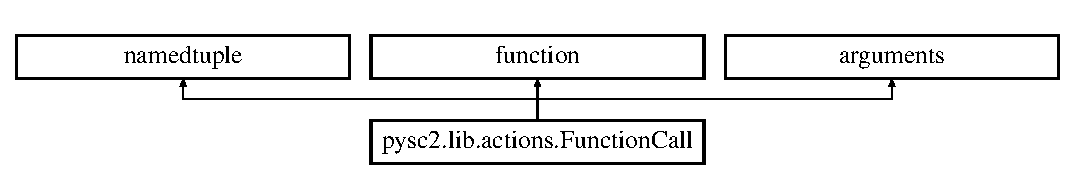
\includegraphics[height=1.964912cm]{classpysc2_1_1lib_1_1actions_1_1_function_call}
\end{center}
\end{figure}
\subsection*{Public Member Functions}
\begin{DoxyCompactItemize}
\item 
def \mbox{\hyperlink{classpysc2_1_1lib_1_1actions_1_1_function_call_a5b3cf8e14a7b779c05e7b80bbed4181e}{init\+\_\+with\+\_\+validation}} (cls, function, arguments)
\item 
def \mbox{\hyperlink{classpysc2_1_1lib_1_1actions_1_1_function_call_a87d05030588a84efaa0c399fe68c3cde}{all\+\_\+arguments}} (cls, function, arguments)
\end{DoxyCompactItemize}


\subsection{Detailed Description}
\begin{DoxyVerb}Represents a function call action.

Attributes:
  function: Store the function id, eg 2 for select_point.
  arguments: The list of arguments for that function, each being a list of
      ints. For select_point this could be: [[0], [23, 38]].
\end{DoxyVerb}
 

\subsection{Member Function Documentation}
\mbox{\Hypertarget{classpysc2_1_1lib_1_1actions_1_1_function_call_a87d05030588a84efaa0c399fe68c3cde}\label{classpysc2_1_1lib_1_1actions_1_1_function_call_a87d05030588a84efaa0c399fe68c3cde}} 
\index{pysc2\+::lib\+::actions\+::\+Function\+Call@{pysc2\+::lib\+::actions\+::\+Function\+Call}!all\+\_\+arguments@{all\+\_\+arguments}}
\index{all\+\_\+arguments@{all\+\_\+arguments}!pysc2\+::lib\+::actions\+::\+Function\+Call@{pysc2\+::lib\+::actions\+::\+Function\+Call}}
\subsubsection{\texorpdfstring{all\+\_\+arguments()}{all\_arguments()}}
{\footnotesize\ttfamily def pysc2.\+lib.\+actions.\+Function\+Call.\+all\+\_\+arguments (\begin{DoxyParamCaption}\item[{}]{cls,  }\item[{}]{function,  }\item[{}]{arguments }\end{DoxyParamCaption})}

\begin{DoxyVerb}Helper function for creating `FunctionCall`s with `Arguments`.

Args:
  function: The value to store for the action function.
  arguments: The values to store for the arguments of the action. Can either
be an `Arguments` object, a `dict`, or an iterable. If a `dict` or an
iterable is provided, the values will be unpacked into an `Arguments`
object.

Returns:
  A new `FunctionCall` instance.
\end{DoxyVerb}
 \mbox{\Hypertarget{classpysc2_1_1lib_1_1actions_1_1_function_call_a5b3cf8e14a7b779c05e7b80bbed4181e}\label{classpysc2_1_1lib_1_1actions_1_1_function_call_a5b3cf8e14a7b779c05e7b80bbed4181e}} 
\index{pysc2\+::lib\+::actions\+::\+Function\+Call@{pysc2\+::lib\+::actions\+::\+Function\+Call}!init\+\_\+with\+\_\+validation@{init\+\_\+with\+\_\+validation}}
\index{init\+\_\+with\+\_\+validation@{init\+\_\+with\+\_\+validation}!pysc2\+::lib\+::actions\+::\+Function\+Call@{pysc2\+::lib\+::actions\+::\+Function\+Call}}
\subsubsection{\texorpdfstring{init\+\_\+with\+\_\+validation()}{init\_with\_validation()}}
{\footnotesize\ttfamily def pysc2.\+lib.\+actions.\+Function\+Call.\+init\+\_\+with\+\_\+validation (\begin{DoxyParamCaption}\item[{}]{cls,  }\item[{}]{function,  }\item[{}]{arguments }\end{DoxyParamCaption})}

\begin{DoxyVerb}Return a `FunctionCall` given some validation for the function and args.

Args:
  function: A function name or id, to be converted into a function id enum.
  arguments: An iterable of function arguments. Arguments that are enum
  types can be passed by name. Arguments that only take one value (ie
  not a point) don't need to be wrapped in a list.

Returns:
  A new `FunctionCall` instance.

Raises:
  KeyError: if the enum name doesn't exist.
  ValueError: if the enum id doesn't exist.
\end{DoxyVerb}
 

The documentation for this class was generated from the following file\+:\begin{DoxyCompactItemize}
\item 
lib/\mbox{\hyperlink{actions_8py}{actions.\+py}}\end{DoxyCompactItemize}

\hypertarget{classpysc2_1_1lib_1_1actions_1_1_functions}{}\section{pysc2.\+lib.\+actions.\+Functions Class Reference}
\label{classpysc2_1_1lib_1_1actions_1_1_functions}\index{pysc2.\+lib.\+actions.\+Functions@{pysc2.\+lib.\+actions.\+Functions}}
Inheritance diagram for pysc2.\+lib.\+actions.\+Functions\+:\begin{figure}[H]
\begin{center}
\leavevmode
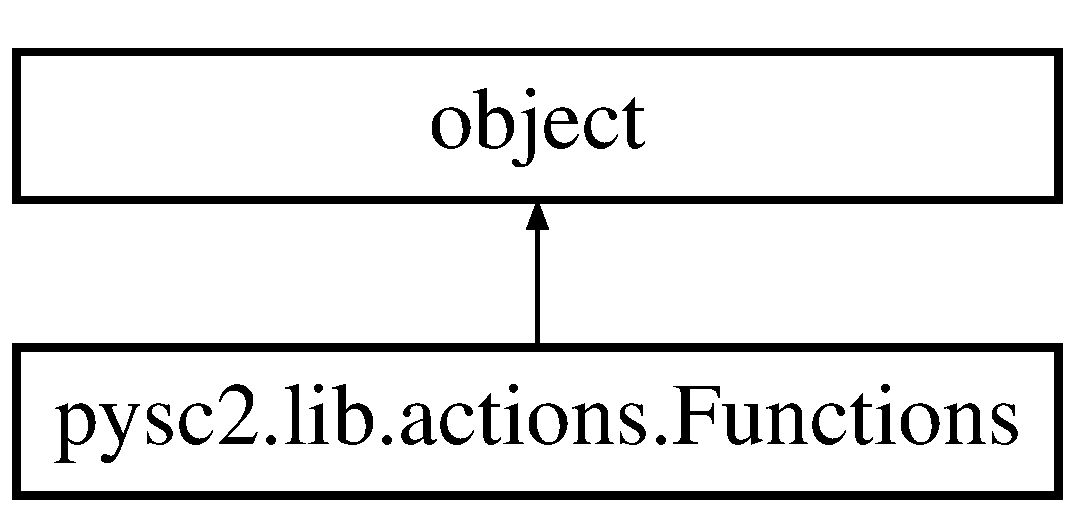
\includegraphics[height=2.000000cm]{classpysc2_1_1lib_1_1actions_1_1_functions}
\end{center}
\end{figure}
\subsection*{Public Member Functions}
\begin{DoxyCompactItemize}
\item 
def \mbox{\hyperlink{classpysc2_1_1lib_1_1actions_1_1_functions_aed31349597035050c81dcd25e5a4e9db}{\+\_\+\+\_\+init\+\_\+\+\_\+}} (self, functions)
\item 
def \mbox{\hyperlink{classpysc2_1_1lib_1_1actions_1_1_functions_a4f7c465199f65341bb825bd63de76e7e}{\+\_\+\+\_\+getattr\+\_\+\+\_\+}} (self, name)
\item 
def \mbox{\hyperlink{classpysc2_1_1lib_1_1actions_1_1_functions_a3a39a75a47ed27754783141ae8089b40}{\+\_\+\+\_\+getitem\+\_\+\+\_\+}} (self, key)
\item 
def \mbox{\hyperlink{classpysc2_1_1lib_1_1actions_1_1_functions_a0b586278648ee7d86ab7636954e441c7}{\+\_\+\+\_\+getstate\+\_\+\+\_\+}} (self)
\item 
def \mbox{\hyperlink{classpysc2_1_1lib_1_1actions_1_1_functions_afeec98d7917f5f74ece2df8d52d53eb5}{\+\_\+\+\_\+setstate\+\_\+\+\_\+}} (self, functions)
\item 
def \mbox{\hyperlink{classpysc2_1_1lib_1_1actions_1_1_functions_ad17534c7035c7516b1605fbd15a9a0d7}{\+\_\+\+\_\+iter\+\_\+\+\_\+}} (self)
\item 
def \mbox{\hyperlink{classpysc2_1_1lib_1_1actions_1_1_functions_a1ec383fa6fb756cb62a584e86b9a756f}{\+\_\+\+\_\+len\+\_\+\+\_\+}} (self)
\item 
def \mbox{\hyperlink{classpysc2_1_1lib_1_1actions_1_1_functions_a44e72099c126871d34471a673b9d23db}{\+\_\+\+\_\+eq\+\_\+\+\_\+}} (self, other)
\end{DoxyCompactItemize}


\subsection{Detailed Description}
\begin{DoxyVerb}Represents the full set of functions.

Can't use namedtuple since python3 has a limit of 255 function arguments, so
build something similar.
\end{DoxyVerb}
 

\subsection{Constructor \& Destructor Documentation}
\mbox{\Hypertarget{classpysc2_1_1lib_1_1actions_1_1_functions_aed31349597035050c81dcd25e5a4e9db}\label{classpysc2_1_1lib_1_1actions_1_1_functions_aed31349597035050c81dcd25e5a4e9db}} 
\index{pysc2\+::lib\+::actions\+::\+Functions@{pysc2\+::lib\+::actions\+::\+Functions}!\+\_\+\+\_\+init\+\_\+\+\_\+@{\+\_\+\+\_\+init\+\_\+\+\_\+}}
\index{\+\_\+\+\_\+init\+\_\+\+\_\+@{\+\_\+\+\_\+init\+\_\+\+\_\+}!pysc2\+::lib\+::actions\+::\+Functions@{pysc2\+::lib\+::actions\+::\+Functions}}
\subsubsection{\texorpdfstring{\+\_\+\+\_\+init\+\_\+\+\_\+()}{\_\_init\_\_()}}
{\footnotesize\ttfamily def pysc2.\+lib.\+actions.\+Functions.\+\_\+\+\_\+init\+\_\+\+\_\+ (\begin{DoxyParamCaption}\item[{}]{self,  }\item[{}]{functions }\end{DoxyParamCaption})}



\subsection{Member Function Documentation}
\mbox{\Hypertarget{classpysc2_1_1lib_1_1actions_1_1_functions_a44e72099c126871d34471a673b9d23db}\label{classpysc2_1_1lib_1_1actions_1_1_functions_a44e72099c126871d34471a673b9d23db}} 
\index{pysc2\+::lib\+::actions\+::\+Functions@{pysc2\+::lib\+::actions\+::\+Functions}!\+\_\+\+\_\+eq\+\_\+\+\_\+@{\+\_\+\+\_\+eq\+\_\+\+\_\+}}
\index{\+\_\+\+\_\+eq\+\_\+\+\_\+@{\+\_\+\+\_\+eq\+\_\+\+\_\+}!pysc2\+::lib\+::actions\+::\+Functions@{pysc2\+::lib\+::actions\+::\+Functions}}
\subsubsection{\texorpdfstring{\+\_\+\+\_\+eq\+\_\+\+\_\+()}{\_\_eq\_\_()}}
{\footnotesize\ttfamily def pysc2.\+lib.\+actions.\+Functions.\+\_\+\+\_\+eq\+\_\+\+\_\+ (\begin{DoxyParamCaption}\item[{}]{self,  }\item[{}]{other }\end{DoxyParamCaption})}

\mbox{\Hypertarget{classpysc2_1_1lib_1_1actions_1_1_functions_a4f7c465199f65341bb825bd63de76e7e}\label{classpysc2_1_1lib_1_1actions_1_1_functions_a4f7c465199f65341bb825bd63de76e7e}} 
\index{pysc2\+::lib\+::actions\+::\+Functions@{pysc2\+::lib\+::actions\+::\+Functions}!\+\_\+\+\_\+getattr\+\_\+\+\_\+@{\+\_\+\+\_\+getattr\+\_\+\+\_\+}}
\index{\+\_\+\+\_\+getattr\+\_\+\+\_\+@{\+\_\+\+\_\+getattr\+\_\+\+\_\+}!pysc2\+::lib\+::actions\+::\+Functions@{pysc2\+::lib\+::actions\+::\+Functions}}
\subsubsection{\texorpdfstring{\+\_\+\+\_\+getattr\+\_\+\+\_\+()}{\_\_getattr\_\_()}}
{\footnotesize\ttfamily def pysc2.\+lib.\+actions.\+Functions.\+\_\+\+\_\+getattr\+\_\+\+\_\+ (\begin{DoxyParamCaption}\item[{}]{self,  }\item[{}]{name }\end{DoxyParamCaption})}

\mbox{\Hypertarget{classpysc2_1_1lib_1_1actions_1_1_functions_a3a39a75a47ed27754783141ae8089b40}\label{classpysc2_1_1lib_1_1actions_1_1_functions_a3a39a75a47ed27754783141ae8089b40}} 
\index{pysc2\+::lib\+::actions\+::\+Functions@{pysc2\+::lib\+::actions\+::\+Functions}!\+\_\+\+\_\+getitem\+\_\+\+\_\+@{\+\_\+\+\_\+getitem\+\_\+\+\_\+}}
\index{\+\_\+\+\_\+getitem\+\_\+\+\_\+@{\+\_\+\+\_\+getitem\+\_\+\+\_\+}!pysc2\+::lib\+::actions\+::\+Functions@{pysc2\+::lib\+::actions\+::\+Functions}}
\subsubsection{\texorpdfstring{\+\_\+\+\_\+getitem\+\_\+\+\_\+()}{\_\_getitem\_\_()}}
{\footnotesize\ttfamily def pysc2.\+lib.\+actions.\+Functions.\+\_\+\+\_\+getitem\+\_\+\+\_\+ (\begin{DoxyParamCaption}\item[{}]{self,  }\item[{}]{key }\end{DoxyParamCaption})}

\mbox{\Hypertarget{classpysc2_1_1lib_1_1actions_1_1_functions_a0b586278648ee7d86ab7636954e441c7}\label{classpysc2_1_1lib_1_1actions_1_1_functions_a0b586278648ee7d86ab7636954e441c7}} 
\index{pysc2\+::lib\+::actions\+::\+Functions@{pysc2\+::lib\+::actions\+::\+Functions}!\+\_\+\+\_\+getstate\+\_\+\+\_\+@{\+\_\+\+\_\+getstate\+\_\+\+\_\+}}
\index{\+\_\+\+\_\+getstate\+\_\+\+\_\+@{\+\_\+\+\_\+getstate\+\_\+\+\_\+}!pysc2\+::lib\+::actions\+::\+Functions@{pysc2\+::lib\+::actions\+::\+Functions}}
\subsubsection{\texorpdfstring{\+\_\+\+\_\+getstate\+\_\+\+\_\+()}{\_\_getstate\_\_()}}
{\footnotesize\ttfamily def pysc2.\+lib.\+actions.\+Functions.\+\_\+\+\_\+getstate\+\_\+\+\_\+ (\begin{DoxyParamCaption}\item[{}]{self }\end{DoxyParamCaption})}

\mbox{\Hypertarget{classpysc2_1_1lib_1_1actions_1_1_functions_ad17534c7035c7516b1605fbd15a9a0d7}\label{classpysc2_1_1lib_1_1actions_1_1_functions_ad17534c7035c7516b1605fbd15a9a0d7}} 
\index{pysc2\+::lib\+::actions\+::\+Functions@{pysc2\+::lib\+::actions\+::\+Functions}!\+\_\+\+\_\+iter\+\_\+\+\_\+@{\+\_\+\+\_\+iter\+\_\+\+\_\+}}
\index{\+\_\+\+\_\+iter\+\_\+\+\_\+@{\+\_\+\+\_\+iter\+\_\+\+\_\+}!pysc2\+::lib\+::actions\+::\+Functions@{pysc2\+::lib\+::actions\+::\+Functions}}
\subsubsection{\texorpdfstring{\+\_\+\+\_\+iter\+\_\+\+\_\+()}{\_\_iter\_\_()}}
{\footnotesize\ttfamily def pysc2.\+lib.\+actions.\+Functions.\+\_\+\+\_\+iter\+\_\+\+\_\+ (\begin{DoxyParamCaption}\item[{}]{self }\end{DoxyParamCaption})}

\mbox{\Hypertarget{classpysc2_1_1lib_1_1actions_1_1_functions_a1ec383fa6fb756cb62a584e86b9a756f}\label{classpysc2_1_1lib_1_1actions_1_1_functions_a1ec383fa6fb756cb62a584e86b9a756f}} 
\index{pysc2\+::lib\+::actions\+::\+Functions@{pysc2\+::lib\+::actions\+::\+Functions}!\+\_\+\+\_\+len\+\_\+\+\_\+@{\+\_\+\+\_\+len\+\_\+\+\_\+}}
\index{\+\_\+\+\_\+len\+\_\+\+\_\+@{\+\_\+\+\_\+len\+\_\+\+\_\+}!pysc2\+::lib\+::actions\+::\+Functions@{pysc2\+::lib\+::actions\+::\+Functions}}
\subsubsection{\texorpdfstring{\+\_\+\+\_\+len\+\_\+\+\_\+()}{\_\_len\_\_()}}
{\footnotesize\ttfamily def pysc2.\+lib.\+actions.\+Functions.\+\_\+\+\_\+len\+\_\+\+\_\+ (\begin{DoxyParamCaption}\item[{}]{self }\end{DoxyParamCaption})}

\mbox{\Hypertarget{classpysc2_1_1lib_1_1actions_1_1_functions_afeec98d7917f5f74ece2df8d52d53eb5}\label{classpysc2_1_1lib_1_1actions_1_1_functions_afeec98d7917f5f74ece2df8d52d53eb5}} 
\index{pysc2\+::lib\+::actions\+::\+Functions@{pysc2\+::lib\+::actions\+::\+Functions}!\+\_\+\+\_\+setstate\+\_\+\+\_\+@{\+\_\+\+\_\+setstate\+\_\+\+\_\+}}
\index{\+\_\+\+\_\+setstate\+\_\+\+\_\+@{\+\_\+\+\_\+setstate\+\_\+\+\_\+}!pysc2\+::lib\+::actions\+::\+Functions@{pysc2\+::lib\+::actions\+::\+Functions}}
\subsubsection{\texorpdfstring{\+\_\+\+\_\+setstate\+\_\+\+\_\+()}{\_\_setstate\_\_()}}
{\footnotesize\ttfamily def pysc2.\+lib.\+actions.\+Functions.\+\_\+\+\_\+setstate\+\_\+\+\_\+ (\begin{DoxyParamCaption}\item[{}]{self,  }\item[{}]{functions }\end{DoxyParamCaption})}



The documentation for this class was generated from the following file\+:\begin{DoxyCompactItemize}
\item 
lib/\mbox{\hyperlink{actions_8py}{actions.\+py}}\end{DoxyCompactItemize}

\hypertarget{classpysc2_1_1tests_1_1replay__obs__test_1_1_game_controller}{}\section{pysc2.\+tests.\+replay\+\_\+obs\+\_\+test.\+Game\+Controller Class Reference}
\label{classpysc2_1_1tests_1_1replay__obs__test_1_1_game_controller}\index{pysc2.\+tests.\+replay\+\_\+obs\+\_\+test.\+Game\+Controller@{pysc2.\+tests.\+replay\+\_\+obs\+\_\+test.\+Game\+Controller}}
Inheritance diagram for pysc2.\+tests.\+replay\+\_\+obs\+\_\+test.\+Game\+Controller\+:\begin{figure}[H]
\begin{center}
\leavevmode
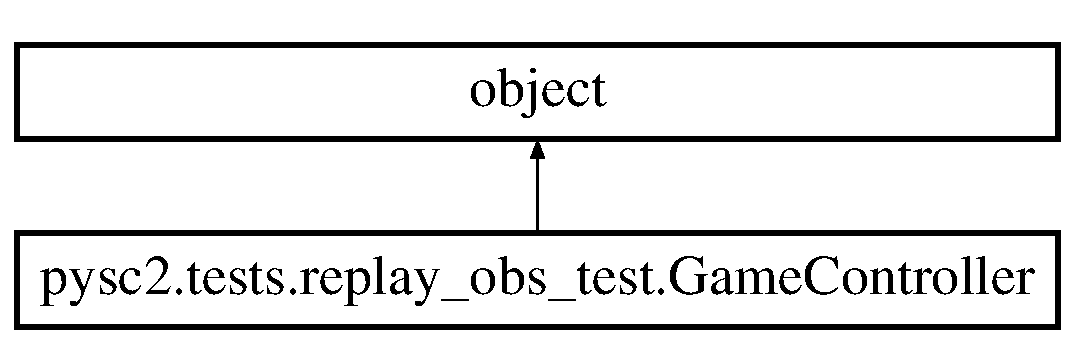
\includegraphics[height=2.000000cm]{classpysc2_1_1tests_1_1replay__obs__test_1_1_game_controller}
\end{center}
\end{figure}
\subsection*{Public Member Functions}
\begin{DoxyCompactItemize}
\item 
def \mbox{\hyperlink{classpysc2_1_1tests_1_1replay__obs__test_1_1_game_controller_a0170d78080a4f367923de5bf0c3af971}{\+\_\+\+\_\+init\+\_\+\+\_\+}} (self, config)
\item 
def \mbox{\hyperlink{classpysc2_1_1tests_1_1replay__obs__test_1_1_game_controller_a591d23a08b084f10396ac70e026c28d6}{start\+\_\+replay}} (self, replay\+\_\+data)
\item 
def \mbox{\hyperlink{classpysc2_1_1tests_1_1replay__obs__test_1_1_game_controller_abc04f315338ca168e4842adbb5630edf}{create\+\_\+game}} (self)
\item 
def \mbox{\hyperlink{classpysc2_1_1tests_1_1replay__obs__test_1_1_game_controller_ab27035af6ebc2cb4d6f4ebe2be77a4d0}{controller}} (self)
\item 
def \mbox{\hyperlink{classpysc2_1_1tests_1_1replay__obs__test_1_1_game_controller_a6a992991922f1fac442c416dc270ddd5}{close}} (self)
\item 
def \mbox{\hyperlink{classpysc2_1_1tests_1_1replay__obs__test_1_1_game_controller_a40610f359f2f40a60a058e1b627d0cad}{\+\_\+\+\_\+enter\+\_\+\+\_\+}} (self)
\item 
def \mbox{\hyperlink{classpysc2_1_1tests_1_1replay__obs__test_1_1_game_controller_a9bd1fb5761643766047cea7af01a47f4}{\+\_\+\+\_\+exit\+\_\+\+\_\+}} (self, exception\+\_\+type, exception\+\_\+value, traceback)
\end{DoxyCompactItemize}


\subsection{Detailed Description}
\begin{DoxyVerb}Wrapper class for interacting with the game in play/replay mode.\end{DoxyVerb}
 

\subsection{Constructor \& Destructor Documentation}
\mbox{\Hypertarget{classpysc2_1_1tests_1_1replay__obs__test_1_1_game_controller_a0170d78080a4f367923de5bf0c3af971}\label{classpysc2_1_1tests_1_1replay__obs__test_1_1_game_controller_a0170d78080a4f367923de5bf0c3af971}} 
\index{pysc2\+::tests\+::replay\+\_\+obs\+\_\+test\+::\+Game\+Controller@{pysc2\+::tests\+::replay\+\_\+obs\+\_\+test\+::\+Game\+Controller}!\+\_\+\+\_\+init\+\_\+\+\_\+@{\+\_\+\+\_\+init\+\_\+\+\_\+}}
\index{\+\_\+\+\_\+init\+\_\+\+\_\+@{\+\_\+\+\_\+init\+\_\+\+\_\+}!pysc2\+::tests\+::replay\+\_\+obs\+\_\+test\+::\+Game\+Controller@{pysc2\+::tests\+::replay\+\_\+obs\+\_\+test\+::\+Game\+Controller}}
\subsubsection{\texorpdfstring{\+\_\+\+\_\+init\+\_\+\+\_\+()}{\_\_init\_\_()}}
{\footnotesize\ttfamily def pysc2.\+tests.\+replay\+\_\+obs\+\_\+test.\+Game\+Controller.\+\_\+\+\_\+init\+\_\+\+\_\+ (\begin{DoxyParamCaption}\item[{}]{self,  }\item[{}]{config }\end{DoxyParamCaption})}

\begin{DoxyVerb}Constructs the game controller object.

Args:
  config: Interface configuration options.
\end{DoxyVerb}
 

\subsection{Member Function Documentation}
\mbox{\Hypertarget{classpysc2_1_1tests_1_1replay__obs__test_1_1_game_controller_a40610f359f2f40a60a058e1b627d0cad}\label{classpysc2_1_1tests_1_1replay__obs__test_1_1_game_controller_a40610f359f2f40a60a058e1b627d0cad}} 
\index{pysc2\+::tests\+::replay\+\_\+obs\+\_\+test\+::\+Game\+Controller@{pysc2\+::tests\+::replay\+\_\+obs\+\_\+test\+::\+Game\+Controller}!\+\_\+\+\_\+enter\+\_\+\+\_\+@{\+\_\+\+\_\+enter\+\_\+\+\_\+}}
\index{\+\_\+\+\_\+enter\+\_\+\+\_\+@{\+\_\+\+\_\+enter\+\_\+\+\_\+}!pysc2\+::tests\+::replay\+\_\+obs\+\_\+test\+::\+Game\+Controller@{pysc2\+::tests\+::replay\+\_\+obs\+\_\+test\+::\+Game\+Controller}}
\subsubsection{\texorpdfstring{\+\_\+\+\_\+enter\+\_\+\+\_\+()}{\_\_enter\_\_()}}
{\footnotesize\ttfamily def pysc2.\+tests.\+replay\+\_\+obs\+\_\+test.\+Game\+Controller.\+\_\+\+\_\+enter\+\_\+\+\_\+ (\begin{DoxyParamCaption}\item[{}]{self }\end{DoxyParamCaption})}

\mbox{\Hypertarget{classpysc2_1_1tests_1_1replay__obs__test_1_1_game_controller_a9bd1fb5761643766047cea7af01a47f4}\label{classpysc2_1_1tests_1_1replay__obs__test_1_1_game_controller_a9bd1fb5761643766047cea7af01a47f4}} 
\index{pysc2\+::tests\+::replay\+\_\+obs\+\_\+test\+::\+Game\+Controller@{pysc2\+::tests\+::replay\+\_\+obs\+\_\+test\+::\+Game\+Controller}!\+\_\+\+\_\+exit\+\_\+\+\_\+@{\+\_\+\+\_\+exit\+\_\+\+\_\+}}
\index{\+\_\+\+\_\+exit\+\_\+\+\_\+@{\+\_\+\+\_\+exit\+\_\+\+\_\+}!pysc2\+::tests\+::replay\+\_\+obs\+\_\+test\+::\+Game\+Controller@{pysc2\+::tests\+::replay\+\_\+obs\+\_\+test\+::\+Game\+Controller}}
\subsubsection{\texorpdfstring{\+\_\+\+\_\+exit\+\_\+\+\_\+()}{\_\_exit\_\_()}}
{\footnotesize\ttfamily def pysc2.\+tests.\+replay\+\_\+obs\+\_\+test.\+Game\+Controller.\+\_\+\+\_\+exit\+\_\+\+\_\+ (\begin{DoxyParamCaption}\item[{}]{self,  }\item[{}]{exception\+\_\+type,  }\item[{}]{exception\+\_\+value,  }\item[{}]{traceback }\end{DoxyParamCaption})}

\mbox{\Hypertarget{classpysc2_1_1tests_1_1replay__obs__test_1_1_game_controller_a6a992991922f1fac442c416dc270ddd5}\label{classpysc2_1_1tests_1_1replay__obs__test_1_1_game_controller_a6a992991922f1fac442c416dc270ddd5}} 
\index{pysc2\+::tests\+::replay\+\_\+obs\+\_\+test\+::\+Game\+Controller@{pysc2\+::tests\+::replay\+\_\+obs\+\_\+test\+::\+Game\+Controller}!close@{close}}
\index{close@{close}!pysc2\+::tests\+::replay\+\_\+obs\+\_\+test\+::\+Game\+Controller@{pysc2\+::tests\+::replay\+\_\+obs\+\_\+test\+::\+Game\+Controller}}
\subsubsection{\texorpdfstring{close()}{close()}}
{\footnotesize\ttfamily def pysc2.\+tests.\+replay\+\_\+obs\+\_\+test.\+Game\+Controller.\+close (\begin{DoxyParamCaption}\item[{}]{self }\end{DoxyParamCaption})}

\begin{DoxyVerb}Close the controller connection.\end{DoxyVerb}
 \mbox{\Hypertarget{classpysc2_1_1tests_1_1replay__obs__test_1_1_game_controller_ab27035af6ebc2cb4d6f4ebe2be77a4d0}\label{classpysc2_1_1tests_1_1replay__obs__test_1_1_game_controller_ab27035af6ebc2cb4d6f4ebe2be77a4d0}} 
\index{pysc2\+::tests\+::replay\+\_\+obs\+\_\+test\+::\+Game\+Controller@{pysc2\+::tests\+::replay\+\_\+obs\+\_\+test\+::\+Game\+Controller}!controller@{controller}}
\index{controller@{controller}!pysc2\+::tests\+::replay\+\_\+obs\+\_\+test\+::\+Game\+Controller@{pysc2\+::tests\+::replay\+\_\+obs\+\_\+test\+::\+Game\+Controller}}
\subsubsection{\texorpdfstring{controller()}{controller()}}
{\footnotesize\ttfamily def pysc2.\+tests.\+replay\+\_\+obs\+\_\+test.\+Game\+Controller.\+controller (\begin{DoxyParamCaption}\item[{}]{self }\end{DoxyParamCaption})}

\mbox{\Hypertarget{classpysc2_1_1tests_1_1replay__obs__test_1_1_game_controller_abc04f315338ca168e4842adbb5630edf}\label{classpysc2_1_1tests_1_1replay__obs__test_1_1_game_controller_abc04f315338ca168e4842adbb5630edf}} 
\index{pysc2\+::tests\+::replay\+\_\+obs\+\_\+test\+::\+Game\+Controller@{pysc2\+::tests\+::replay\+\_\+obs\+\_\+test\+::\+Game\+Controller}!create\+\_\+game@{create\+\_\+game}}
\index{create\+\_\+game@{create\+\_\+game}!pysc2\+::tests\+::replay\+\_\+obs\+\_\+test\+::\+Game\+Controller@{pysc2\+::tests\+::replay\+\_\+obs\+\_\+test\+::\+Game\+Controller}}
\subsubsection{\texorpdfstring{create\+\_\+game()}{create\_game()}}
{\footnotesize\ttfamily def pysc2.\+tests.\+replay\+\_\+obs\+\_\+test.\+Game\+Controller.\+create\+\_\+game (\begin{DoxyParamCaption}\item[{}]{self }\end{DoxyParamCaption})}

\mbox{\Hypertarget{classpysc2_1_1tests_1_1replay__obs__test_1_1_game_controller_a591d23a08b084f10396ac70e026c28d6}\label{classpysc2_1_1tests_1_1replay__obs__test_1_1_game_controller_a591d23a08b084f10396ac70e026c28d6}} 
\index{pysc2\+::tests\+::replay\+\_\+obs\+\_\+test\+::\+Game\+Controller@{pysc2\+::tests\+::replay\+\_\+obs\+\_\+test\+::\+Game\+Controller}!start\+\_\+replay@{start\+\_\+replay}}
\index{start\+\_\+replay@{start\+\_\+replay}!pysc2\+::tests\+::replay\+\_\+obs\+\_\+test\+::\+Game\+Controller@{pysc2\+::tests\+::replay\+\_\+obs\+\_\+test\+::\+Game\+Controller}}
\subsubsection{\texorpdfstring{start\+\_\+replay()}{start\_replay()}}
{\footnotesize\ttfamily def pysc2.\+tests.\+replay\+\_\+obs\+\_\+test.\+Game\+Controller.\+start\+\_\+replay (\begin{DoxyParamCaption}\item[{}]{self,  }\item[{}]{replay\+\_\+data }\end{DoxyParamCaption})}



The documentation for this class was generated from the following file\+:\begin{DoxyCompactItemize}
\item 
tests/\mbox{\hyperlink{replay__obs__test_8py}{replay\+\_\+obs\+\_\+test.\+py}}\end{DoxyCompactItemize}

\hypertarget{classpysc2_1_1maps_1_1ladder_1_1_ladder}{}\section{pysc2.\+maps.\+ladder.\+Ladder Class Reference}
\label{classpysc2_1_1maps_1_1ladder_1_1_ladder}\index{pysc2.\+maps.\+ladder.\+Ladder@{pysc2.\+maps.\+ladder.\+Ladder}}
Inheritance diagram for pysc2.\+maps.\+ladder.\+Ladder\+:\begin{figure}[H]
\begin{center}
\leavevmode
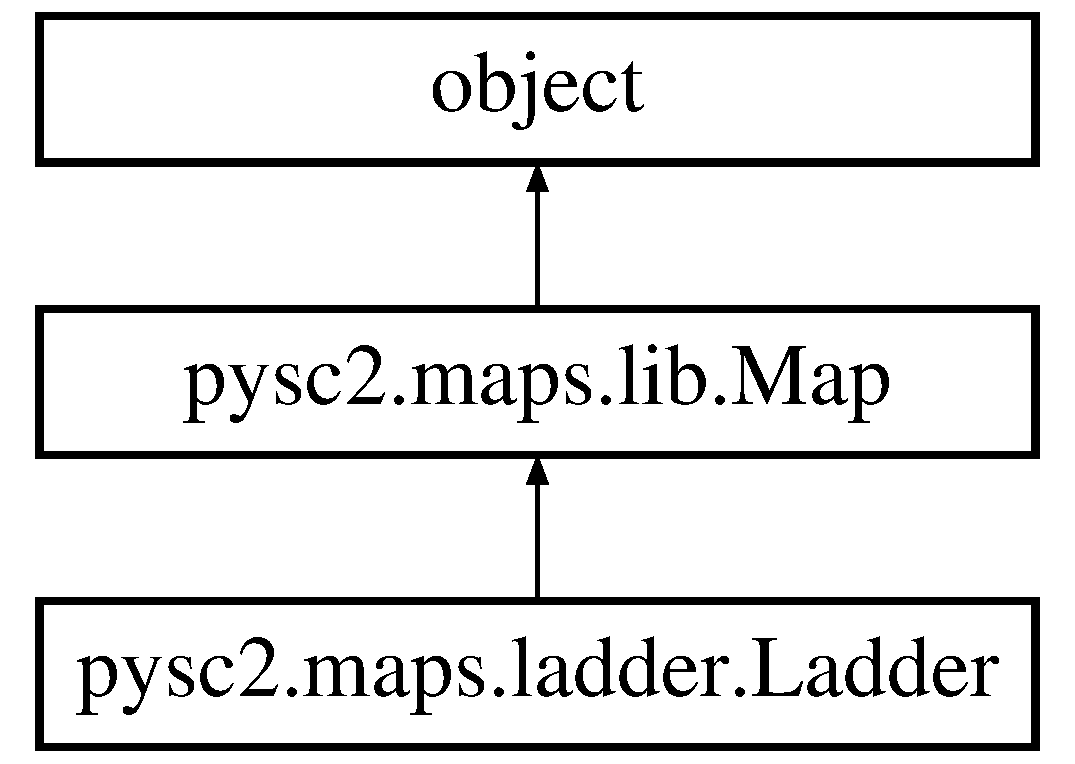
\includegraphics[height=3.000000cm]{classpysc2_1_1maps_1_1ladder_1_1_ladder}
\end{center}
\end{figure}
\subsection*{Static Public Attributes}
\begin{DoxyCompactItemize}
\item 
int \mbox{\hyperlink{classpysc2_1_1maps_1_1ladder_1_1_ladder_a6be765133191a3368339407980256040}{players}} = 2
\item 
int \mbox{\hyperlink{classpysc2_1_1maps_1_1ladder_1_1_ladder_ab08a3654622ac11be5c69543ca974d31}{game\+\_\+steps\+\_\+per\+\_\+episode}} = 16 $\ast$ 60 $\ast$ 30
\item 
string \mbox{\hyperlink{classpysc2_1_1maps_1_1ladder_1_1_ladder_aa001b72aeee3c8fb4a293a8577d24fb7}{download}} = \char`\"{}https\+://github.\+com/Blizzard/s2client-\/proto\#map-\/packs\char`\"{}
\end{DoxyCompactItemize}
\subsection*{Additional Inherited Members}


\subsection{Member Data Documentation}
\mbox{\Hypertarget{classpysc2_1_1maps_1_1ladder_1_1_ladder_aa001b72aeee3c8fb4a293a8577d24fb7}\label{classpysc2_1_1maps_1_1ladder_1_1_ladder_aa001b72aeee3c8fb4a293a8577d24fb7}} 
\index{pysc2\+::maps\+::ladder\+::\+Ladder@{pysc2\+::maps\+::ladder\+::\+Ladder}!download@{download}}
\index{download@{download}!pysc2\+::maps\+::ladder\+::\+Ladder@{pysc2\+::maps\+::ladder\+::\+Ladder}}
\subsubsection{\texorpdfstring{download}{download}}
{\footnotesize\ttfamily string pysc2.\+maps.\+ladder.\+Ladder.\+download = \char`\"{}https\+://github.\+com/Blizzard/s2client-\/proto\#map-\/packs\char`\"{}\hspace{0.3cm}{\ttfamily [static]}}

\mbox{\Hypertarget{classpysc2_1_1maps_1_1ladder_1_1_ladder_ab08a3654622ac11be5c69543ca974d31}\label{classpysc2_1_1maps_1_1ladder_1_1_ladder_ab08a3654622ac11be5c69543ca974d31}} 
\index{pysc2\+::maps\+::ladder\+::\+Ladder@{pysc2\+::maps\+::ladder\+::\+Ladder}!game\+\_\+steps\+\_\+per\+\_\+episode@{game\+\_\+steps\+\_\+per\+\_\+episode}}
\index{game\+\_\+steps\+\_\+per\+\_\+episode@{game\+\_\+steps\+\_\+per\+\_\+episode}!pysc2\+::maps\+::ladder\+::\+Ladder@{pysc2\+::maps\+::ladder\+::\+Ladder}}
\subsubsection{\texorpdfstring{game\+\_\+steps\+\_\+per\+\_\+episode}{game\_steps\_per\_episode}}
{\footnotesize\ttfamily int pysc2.\+maps.\+ladder.\+Ladder.\+game\+\_\+steps\+\_\+per\+\_\+episode = 16 $\ast$ 60 $\ast$ 30\hspace{0.3cm}{\ttfamily [static]}}

\mbox{\Hypertarget{classpysc2_1_1maps_1_1ladder_1_1_ladder_a6be765133191a3368339407980256040}\label{classpysc2_1_1maps_1_1ladder_1_1_ladder_a6be765133191a3368339407980256040}} 
\index{pysc2\+::maps\+::ladder\+::\+Ladder@{pysc2\+::maps\+::ladder\+::\+Ladder}!players@{players}}
\index{players@{players}!pysc2\+::maps\+::ladder\+::\+Ladder@{pysc2\+::maps\+::ladder\+::\+Ladder}}
\subsubsection{\texorpdfstring{players}{players}}
{\footnotesize\ttfamily int pysc2.\+maps.\+ladder.\+Ladder.\+players = 2\hspace{0.3cm}{\ttfamily [static]}}



The documentation for this class was generated from the following file\+:\begin{DoxyCompactItemize}
\item 
maps/\mbox{\hyperlink{ladder_8py}{ladder.\+py}}\end{DoxyCompactItemize}

\hypertarget{classpysc2_1_1env_1_1lan__sc2__env_1_1_lan_s_c2_env}{}\section{pysc2.\+env.\+lan\+\_\+sc2\+\_\+env.\+Lan\+S\+C2\+Env Class Reference}
\label{classpysc2_1_1env_1_1lan__sc2__env_1_1_lan_s_c2_env}\index{pysc2.\+env.\+lan\+\_\+sc2\+\_\+env.\+Lan\+S\+C2\+Env@{pysc2.\+env.\+lan\+\_\+sc2\+\_\+env.\+Lan\+S\+C2\+Env}}
Inheritance diagram for pysc2.\+env.\+lan\+\_\+sc2\+\_\+env.\+Lan\+S\+C2\+Env\+:\begin{figure}[H]
\begin{center}
\leavevmode
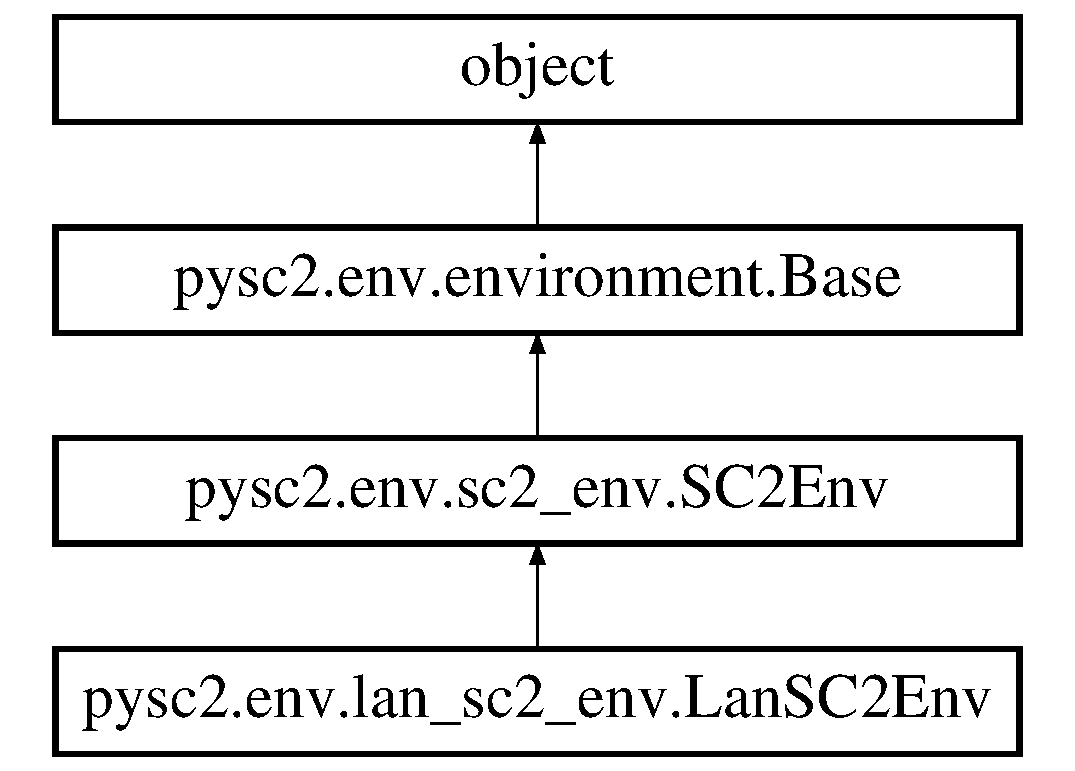
\includegraphics[height=4.000000cm]{classpysc2_1_1env_1_1lan__sc2__env_1_1_lan_s_c2_env}
\end{center}
\end{figure}
\subsection*{Public Member Functions}
\begin{DoxyCompactItemize}
\item 
def \mbox{\hyperlink{classpysc2_1_1env_1_1lan__sc2__env_1_1_lan_s_c2_env_af811660c93bbe7d4660fcdc7317bb57f}{\+\_\+\+\_\+init\+\_\+\+\_\+}} (self, \+\_\+only\+\_\+use\+\_\+kwargs=None, host=\char`\"{}127.\+0.\+0.\+1\char`\"{}, config\+\_\+port=None, race=None, agent\+\_\+interface\+\_\+format=None, discount=1., visualize=False, step\+\_\+mul=None, replay\+\_\+dir=None)
\item 
def \mbox{\hyperlink{classpysc2_1_1env_1_1lan__sc2__env_1_1_lan_s_c2_env_afe3313585911c165f7128cb6c8afa21f}{close}} (self)
\end{DoxyCompactItemize}


\subsection{Detailed Description}
\begin{DoxyVerb}A Starcraft II environment for playing vs humans over LAN.

This owns a single instance, and expects to join a game hosted by some other
script, likely play_vs_agent.py.
\end{DoxyVerb}
 

\subsection{Constructor \& Destructor Documentation}
\mbox{\Hypertarget{classpysc2_1_1env_1_1lan__sc2__env_1_1_lan_s_c2_env_af811660c93bbe7d4660fcdc7317bb57f}\label{classpysc2_1_1env_1_1lan__sc2__env_1_1_lan_s_c2_env_af811660c93bbe7d4660fcdc7317bb57f}} 
\index{pysc2\+::env\+::lan\+\_\+sc2\+\_\+env\+::\+Lan\+S\+C2\+Env@{pysc2\+::env\+::lan\+\_\+sc2\+\_\+env\+::\+Lan\+S\+C2\+Env}!\+\_\+\+\_\+init\+\_\+\+\_\+@{\+\_\+\+\_\+init\+\_\+\+\_\+}}
\index{\+\_\+\+\_\+init\+\_\+\+\_\+@{\+\_\+\+\_\+init\+\_\+\+\_\+}!pysc2\+::env\+::lan\+\_\+sc2\+\_\+env\+::\+Lan\+S\+C2\+Env@{pysc2\+::env\+::lan\+\_\+sc2\+\_\+env\+::\+Lan\+S\+C2\+Env}}
\subsubsection{\texorpdfstring{\+\_\+\+\_\+init\+\_\+\+\_\+()}{\_\_init\_\_()}}
{\footnotesize\ttfamily def pysc2.\+env.\+lan\+\_\+sc2\+\_\+env.\+Lan\+S\+C2\+Env.\+\_\+\+\_\+init\+\_\+\+\_\+ (\begin{DoxyParamCaption}\item[{}]{self,  }\item[{}]{\+\_\+only\+\_\+use\+\_\+kwargs = {\ttfamily None},  }\item[{}]{host = {\ttfamily \char`\"{}127.0.0.1\char`\"{}},  }\item[{}]{config\+\_\+port = {\ttfamily None},  }\item[{}]{race = {\ttfamily None},  }\item[{}]{agent\+\_\+interface\+\_\+format = {\ttfamily None},  }\item[{}]{discount = {\ttfamily 1.},  }\item[{}]{visualize = {\ttfamily False},  }\item[{}]{step\+\_\+mul = {\ttfamily None},  }\item[{}]{replay\+\_\+dir = {\ttfamily None} }\end{DoxyParamCaption})}

\begin{DoxyVerb}Create a SC2 Env that connects to a remote instance of the game.

This assumes that the game is already up and running, and it only needs to
join. You need some other script to launch the process and call
RequestCreateGame. It also assumes that it's a multiplayer game, and that
the ports are consecutive.

You must pass a resolution that you want to play at. You can send either
feature layer resolution or rgb resolution or both. If you send both you
must also choose which to use as your action space. Regardless of which you
choose you must send both the screen and minimap resolutions.

For each of the 4 resolutions, either specify size or both width and
height. If you specify size then both width and height will take that value.

Args:
  _only_use_kwargs: Don't pass args, only kwargs.
  host: Which ip to use. Either ipv4 or ipv6 localhost.
  config_port: Where to find the config port.
  race: Race for this agent.
  agent_interface_format: AgentInterfaceFormat object describing the
  format of communication between the agent and the environment.
  discount: Returned as part of the observation.
  visualize: Whether to pop up a window showing the camera and feature
  layers. This won't work without access to a window manager.
  step_mul: How many game steps per agent step (action/observation). None
  means use the map default.
  replay_dir: Directory to save a replay.

Raises:
  ValueError: if the race is invalid.
  ValueError: if the resolutions aren't specified correctly.
  ValueError: if the host or port are invalid.
\end{DoxyVerb}
 

\subsection{Member Function Documentation}
\mbox{\Hypertarget{classpysc2_1_1env_1_1lan__sc2__env_1_1_lan_s_c2_env_afe3313585911c165f7128cb6c8afa21f}\label{classpysc2_1_1env_1_1lan__sc2__env_1_1_lan_s_c2_env_afe3313585911c165f7128cb6c8afa21f}} 
\index{pysc2\+::env\+::lan\+\_\+sc2\+\_\+env\+::\+Lan\+S\+C2\+Env@{pysc2\+::env\+::lan\+\_\+sc2\+\_\+env\+::\+Lan\+S\+C2\+Env}!close@{close}}
\index{close@{close}!pysc2\+::env\+::lan\+\_\+sc2\+\_\+env\+::\+Lan\+S\+C2\+Env@{pysc2\+::env\+::lan\+\_\+sc2\+\_\+env\+::\+Lan\+S\+C2\+Env}}
\subsubsection{\texorpdfstring{close()}{close()}}
{\footnotesize\ttfamily def pysc2.\+env.\+lan\+\_\+sc2\+\_\+env.\+Lan\+S\+C2\+Env.\+close (\begin{DoxyParamCaption}\item[{}]{self }\end{DoxyParamCaption})}



The documentation for this class was generated from the following file\+:\begin{DoxyCompactItemize}
\item 
env/\mbox{\hyperlink{lan__sc2__env_8py}{lan\+\_\+sc2\+\_\+env.\+py}}\end{DoxyCompactItemize}

\hypertarget{classpysc2_1_1lib_1_1transform_1_1_linear}{}\section{pysc2.\+lib.\+transform.\+Linear Class Reference}
\label{classpysc2_1_1lib_1_1transform_1_1_linear}\index{pysc2.\+lib.\+transform.\+Linear@{pysc2.\+lib.\+transform.\+Linear}}
Inheritance diagram for pysc2.\+lib.\+transform.\+Linear\+:\begin{figure}[H]
\begin{center}
\leavevmode
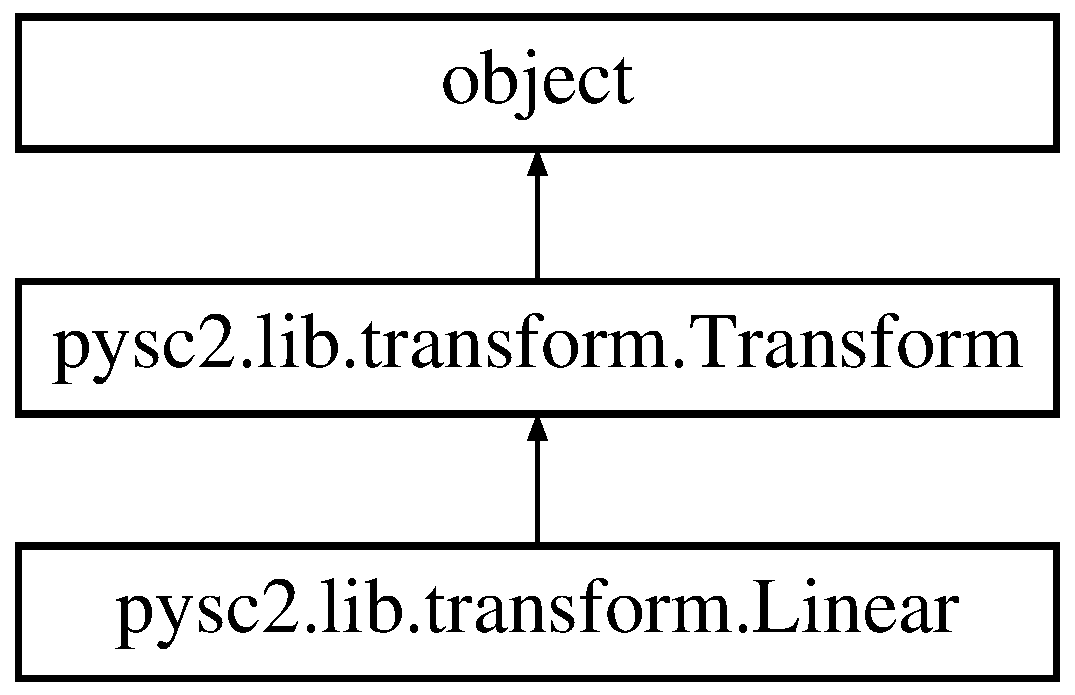
\includegraphics[height=3.000000cm]{classpysc2_1_1lib_1_1transform_1_1_linear}
\end{center}
\end{figure}
\subsection*{Public Member Functions}
\begin{DoxyCompactItemize}
\item 
def \mbox{\hyperlink{classpysc2_1_1lib_1_1transform_1_1_linear_a06a44d88ea3290ac1e9322188bfe3467}{\+\_\+\+\_\+init\+\_\+\+\_\+}} (self, \mbox{\hyperlink{classpysc2_1_1lib_1_1transform_1_1_linear_ab3878c47278f90e9b5356776e73b517b}{scale}}=None, \mbox{\hyperlink{classpysc2_1_1lib_1_1transform_1_1_linear_a01c3b2d7fafe75ff24327c57e3a684c9}{offset}}=None)
\item 
def \mbox{\hyperlink{classpysc2_1_1lib_1_1transform_1_1_linear_aa540ebc88fcfb5e61bc2516ed5ca3077}{fwd\+\_\+dist}} (self, dist)
\item 
def \mbox{\hyperlink{classpysc2_1_1lib_1_1transform_1_1_linear_ab5b6ab1a2dbfcdbe72e7476d0e6c71e5}{fwd\+\_\+pt}} (self, pt)
\item 
def \mbox{\hyperlink{classpysc2_1_1lib_1_1transform_1_1_linear_a20b03bc9984ab9b5bffb93a157a448d1}{back\+\_\+dist}} (self, dist)
\item 
def \mbox{\hyperlink{classpysc2_1_1lib_1_1transform_1_1_linear_aab8bccdffa1f68f095af071b7cab7471}{back\+\_\+pt}} (self, pt)
\item 
def \mbox{\hyperlink{classpysc2_1_1lib_1_1transform_1_1_linear_a9c94d0303ddc2067febe43ba4ed58192}{\+\_\+\+\_\+str\+\_\+\+\_\+}} (self)
\end{DoxyCompactItemize}
\subsection*{Public Attributes}
\begin{DoxyCompactItemize}
\item 
\mbox{\hyperlink{classpysc2_1_1lib_1_1transform_1_1_linear_ab3878c47278f90e9b5356776e73b517b}{scale}}
\item 
\mbox{\hyperlink{classpysc2_1_1lib_1_1transform_1_1_linear_a01c3b2d7fafe75ff24327c57e3a684c9}{offset}}
\end{DoxyCompactItemize}


\subsection{Detailed Description}
\begin{DoxyVerb}A linear transform with a scale and offset.\end{DoxyVerb}
 

\subsection{Constructor \& Destructor Documentation}
\mbox{\Hypertarget{classpysc2_1_1lib_1_1transform_1_1_linear_a06a44d88ea3290ac1e9322188bfe3467}\label{classpysc2_1_1lib_1_1transform_1_1_linear_a06a44d88ea3290ac1e9322188bfe3467}} 
\index{pysc2\+::lib\+::transform\+::\+Linear@{pysc2\+::lib\+::transform\+::\+Linear}!\+\_\+\+\_\+init\+\_\+\+\_\+@{\+\_\+\+\_\+init\+\_\+\+\_\+}}
\index{\+\_\+\+\_\+init\+\_\+\+\_\+@{\+\_\+\+\_\+init\+\_\+\+\_\+}!pysc2\+::lib\+::transform\+::\+Linear@{pysc2\+::lib\+::transform\+::\+Linear}}
\subsubsection{\texorpdfstring{\+\_\+\+\_\+init\+\_\+\+\_\+()}{\_\_init\_\_()}}
{\footnotesize\ttfamily def pysc2.\+lib.\+transform.\+Linear.\+\_\+\+\_\+init\+\_\+\+\_\+ (\begin{DoxyParamCaption}\item[{}]{self,  }\item[{}]{scale = {\ttfamily None},  }\item[{}]{offset = {\ttfamily None} }\end{DoxyParamCaption})}



\subsection{Member Function Documentation}
\mbox{\Hypertarget{classpysc2_1_1lib_1_1transform_1_1_linear_a9c94d0303ddc2067febe43ba4ed58192}\label{classpysc2_1_1lib_1_1transform_1_1_linear_a9c94d0303ddc2067febe43ba4ed58192}} 
\index{pysc2\+::lib\+::transform\+::\+Linear@{pysc2\+::lib\+::transform\+::\+Linear}!\+\_\+\+\_\+str\+\_\+\+\_\+@{\+\_\+\+\_\+str\+\_\+\+\_\+}}
\index{\+\_\+\+\_\+str\+\_\+\+\_\+@{\+\_\+\+\_\+str\+\_\+\+\_\+}!pysc2\+::lib\+::transform\+::\+Linear@{pysc2\+::lib\+::transform\+::\+Linear}}
\subsubsection{\texorpdfstring{\+\_\+\+\_\+str\+\_\+\+\_\+()}{\_\_str\_\_()}}
{\footnotesize\ttfamily def pysc2.\+lib.\+transform.\+Linear.\+\_\+\+\_\+str\+\_\+\+\_\+ (\begin{DoxyParamCaption}\item[{}]{self }\end{DoxyParamCaption})}

\mbox{\Hypertarget{classpysc2_1_1lib_1_1transform_1_1_linear_a20b03bc9984ab9b5bffb93a157a448d1}\label{classpysc2_1_1lib_1_1transform_1_1_linear_a20b03bc9984ab9b5bffb93a157a448d1}} 
\index{pysc2\+::lib\+::transform\+::\+Linear@{pysc2\+::lib\+::transform\+::\+Linear}!back\+\_\+dist@{back\+\_\+dist}}
\index{back\+\_\+dist@{back\+\_\+dist}!pysc2\+::lib\+::transform\+::\+Linear@{pysc2\+::lib\+::transform\+::\+Linear}}
\subsubsection{\texorpdfstring{back\+\_\+dist()}{back\_dist()}}
{\footnotesize\ttfamily def pysc2.\+lib.\+transform.\+Linear.\+back\+\_\+dist (\begin{DoxyParamCaption}\item[{}]{self,  }\item[{}]{dist }\end{DoxyParamCaption})}

\mbox{\Hypertarget{classpysc2_1_1lib_1_1transform_1_1_linear_aab8bccdffa1f68f095af071b7cab7471}\label{classpysc2_1_1lib_1_1transform_1_1_linear_aab8bccdffa1f68f095af071b7cab7471}} 
\index{pysc2\+::lib\+::transform\+::\+Linear@{pysc2\+::lib\+::transform\+::\+Linear}!back\+\_\+pt@{back\+\_\+pt}}
\index{back\+\_\+pt@{back\+\_\+pt}!pysc2\+::lib\+::transform\+::\+Linear@{pysc2\+::lib\+::transform\+::\+Linear}}
\subsubsection{\texorpdfstring{back\+\_\+pt()}{back\_pt()}}
{\footnotesize\ttfamily def pysc2.\+lib.\+transform.\+Linear.\+back\+\_\+pt (\begin{DoxyParamCaption}\item[{}]{self,  }\item[{}]{pt }\end{DoxyParamCaption})}

\mbox{\Hypertarget{classpysc2_1_1lib_1_1transform_1_1_linear_aa540ebc88fcfb5e61bc2516ed5ca3077}\label{classpysc2_1_1lib_1_1transform_1_1_linear_aa540ebc88fcfb5e61bc2516ed5ca3077}} 
\index{pysc2\+::lib\+::transform\+::\+Linear@{pysc2\+::lib\+::transform\+::\+Linear}!fwd\+\_\+dist@{fwd\+\_\+dist}}
\index{fwd\+\_\+dist@{fwd\+\_\+dist}!pysc2\+::lib\+::transform\+::\+Linear@{pysc2\+::lib\+::transform\+::\+Linear}}
\subsubsection{\texorpdfstring{fwd\+\_\+dist()}{fwd\_dist()}}
{\footnotesize\ttfamily def pysc2.\+lib.\+transform.\+Linear.\+fwd\+\_\+dist (\begin{DoxyParamCaption}\item[{}]{self,  }\item[{}]{dist }\end{DoxyParamCaption})}

\mbox{\Hypertarget{classpysc2_1_1lib_1_1transform_1_1_linear_ab5b6ab1a2dbfcdbe72e7476d0e6c71e5}\label{classpysc2_1_1lib_1_1transform_1_1_linear_ab5b6ab1a2dbfcdbe72e7476d0e6c71e5}} 
\index{pysc2\+::lib\+::transform\+::\+Linear@{pysc2\+::lib\+::transform\+::\+Linear}!fwd\+\_\+pt@{fwd\+\_\+pt}}
\index{fwd\+\_\+pt@{fwd\+\_\+pt}!pysc2\+::lib\+::transform\+::\+Linear@{pysc2\+::lib\+::transform\+::\+Linear}}
\subsubsection{\texorpdfstring{fwd\+\_\+pt()}{fwd\_pt()}}
{\footnotesize\ttfamily def pysc2.\+lib.\+transform.\+Linear.\+fwd\+\_\+pt (\begin{DoxyParamCaption}\item[{}]{self,  }\item[{}]{pt }\end{DoxyParamCaption})}



\subsection{Member Data Documentation}
\mbox{\Hypertarget{classpysc2_1_1lib_1_1transform_1_1_linear_a01c3b2d7fafe75ff24327c57e3a684c9}\label{classpysc2_1_1lib_1_1transform_1_1_linear_a01c3b2d7fafe75ff24327c57e3a684c9}} 
\index{pysc2\+::lib\+::transform\+::\+Linear@{pysc2\+::lib\+::transform\+::\+Linear}!offset@{offset}}
\index{offset@{offset}!pysc2\+::lib\+::transform\+::\+Linear@{pysc2\+::lib\+::transform\+::\+Linear}}
\subsubsection{\texorpdfstring{offset}{offset}}
{\footnotesize\ttfamily pysc2.\+lib.\+transform.\+Linear.\+offset}

\mbox{\Hypertarget{classpysc2_1_1lib_1_1transform_1_1_linear_ab3878c47278f90e9b5356776e73b517b}\label{classpysc2_1_1lib_1_1transform_1_1_linear_ab3878c47278f90e9b5356776e73b517b}} 
\index{pysc2\+::lib\+::transform\+::\+Linear@{pysc2\+::lib\+::transform\+::\+Linear}!scale@{scale}}
\index{scale@{scale}!pysc2\+::lib\+::transform\+::\+Linear@{pysc2\+::lib\+::transform\+::\+Linear}}
\subsubsection{\texorpdfstring{scale}{scale}}
{\footnotesize\ttfamily pysc2.\+lib.\+transform.\+Linear.\+scale}



The documentation for this class was generated from the following file\+:\begin{DoxyCompactItemize}
\item 
lib/\mbox{\hyperlink{transform_8py}{transform.\+py}}\end{DoxyCompactItemize}

\hypertarget{classpysc2_1_1run__configs_1_1platforms_1_1_linux}{}\section{pysc2.\+run\+\_\+configs.\+platforms.\+Linux Class Reference}
\label{classpysc2_1_1run__configs_1_1platforms_1_1_linux}\index{pysc2.\+run\+\_\+configs.\+platforms.\+Linux@{pysc2.\+run\+\_\+configs.\+platforms.\+Linux}}
Inheritance diagram for pysc2.\+run\+\_\+configs.\+platforms.\+Linux\+:\begin{figure}[H]
\begin{center}
\leavevmode
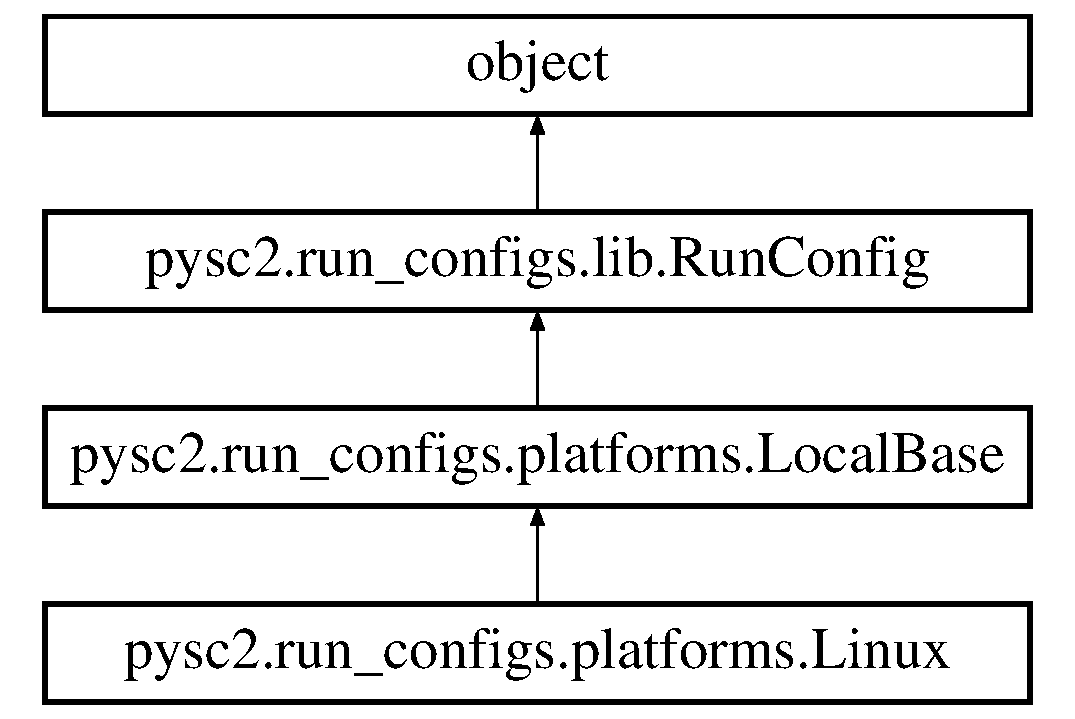
\includegraphics[height=4.000000cm]{classpysc2_1_1run__configs_1_1platforms_1_1_linux}
\end{center}
\end{figure}
\subsection*{Public Member Functions}
\begin{DoxyCompactItemize}
\item 
def \mbox{\hyperlink{classpysc2_1_1run__configs_1_1platforms_1_1_linux_a06f906f71c6cdd07a5249871b24c0aea}{\+\_\+\+\_\+init\+\_\+\+\_\+}} (self)
\item 
def \mbox{\hyperlink{classpysc2_1_1run__configs_1_1platforms_1_1_linux_a2f1c9498e2a28175792e421daa11c5ac}{priority}} (cls)
\item 
def \mbox{\hyperlink{classpysc2_1_1run__configs_1_1platforms_1_1_linux_a266b7d15eb79da465b9d6968398936ea}{start}} (self, kwargs)
\end{DoxyCompactItemize}
\subsection*{Static Public Attributes}
\begin{DoxyCompactItemize}
\item 
list \mbox{\hyperlink{classpysc2_1_1run__configs_1_1platforms_1_1_linux_af3779a9cffe30d5d7f87ffce73a61772}{known\+\_\+mesa}}
\end{DoxyCompactItemize}
\subsection*{Additional Inherited Members}


\subsection{Detailed Description}
\begin{DoxyVerb}Config to run on Linux.\end{DoxyVerb}
 

\subsection{Constructor \& Destructor Documentation}
\mbox{\Hypertarget{classpysc2_1_1run__configs_1_1platforms_1_1_linux_a06f906f71c6cdd07a5249871b24c0aea}\label{classpysc2_1_1run__configs_1_1platforms_1_1_linux_a06f906f71c6cdd07a5249871b24c0aea}} 
\index{pysc2\+::run\+\_\+configs\+::platforms\+::\+Linux@{pysc2\+::run\+\_\+configs\+::platforms\+::\+Linux}!\+\_\+\+\_\+init\+\_\+\+\_\+@{\+\_\+\+\_\+init\+\_\+\+\_\+}}
\index{\+\_\+\+\_\+init\+\_\+\+\_\+@{\+\_\+\+\_\+init\+\_\+\+\_\+}!pysc2\+::run\+\_\+configs\+::platforms\+::\+Linux@{pysc2\+::run\+\_\+configs\+::platforms\+::\+Linux}}
\subsubsection{\texorpdfstring{\+\_\+\+\_\+init\+\_\+\+\_\+()}{\_\_init\_\_()}}
{\footnotesize\ttfamily def pysc2.\+run\+\_\+configs.\+platforms.\+Linux.\+\_\+\+\_\+init\+\_\+\+\_\+ (\begin{DoxyParamCaption}\item[{}]{self }\end{DoxyParamCaption})}



\subsection{Member Function Documentation}
\mbox{\Hypertarget{classpysc2_1_1run__configs_1_1platforms_1_1_linux_a2f1c9498e2a28175792e421daa11c5ac}\label{classpysc2_1_1run__configs_1_1platforms_1_1_linux_a2f1c9498e2a28175792e421daa11c5ac}} 
\index{pysc2\+::run\+\_\+configs\+::platforms\+::\+Linux@{pysc2\+::run\+\_\+configs\+::platforms\+::\+Linux}!priority@{priority}}
\index{priority@{priority}!pysc2\+::run\+\_\+configs\+::platforms\+::\+Linux@{pysc2\+::run\+\_\+configs\+::platforms\+::\+Linux}}
\subsubsection{\texorpdfstring{priority()}{priority()}}
{\footnotesize\ttfamily def pysc2.\+run\+\_\+configs.\+platforms.\+Linux.\+priority (\begin{DoxyParamCaption}\item[{}]{cls }\end{DoxyParamCaption})}

\mbox{\Hypertarget{classpysc2_1_1run__configs_1_1platforms_1_1_linux_a266b7d15eb79da465b9d6968398936ea}\label{classpysc2_1_1run__configs_1_1platforms_1_1_linux_a266b7d15eb79da465b9d6968398936ea}} 
\index{pysc2\+::run\+\_\+configs\+::platforms\+::\+Linux@{pysc2\+::run\+\_\+configs\+::platforms\+::\+Linux}!start@{start}}
\index{start@{start}!pysc2\+::run\+\_\+configs\+::platforms\+::\+Linux@{pysc2\+::run\+\_\+configs\+::platforms\+::\+Linux}}
\subsubsection{\texorpdfstring{start()}{start()}}
{\footnotesize\ttfamily def pysc2.\+run\+\_\+configs.\+platforms.\+Linux.\+start (\begin{DoxyParamCaption}\item[{}]{self,  }\item[{}]{kwargs }\end{DoxyParamCaption})}



\subsection{Member Data Documentation}
\mbox{\Hypertarget{classpysc2_1_1run__configs_1_1platforms_1_1_linux_af3779a9cffe30d5d7f87ffce73a61772}\label{classpysc2_1_1run__configs_1_1platforms_1_1_linux_af3779a9cffe30d5d7f87ffce73a61772}} 
\index{pysc2\+::run\+\_\+configs\+::platforms\+::\+Linux@{pysc2\+::run\+\_\+configs\+::platforms\+::\+Linux}!known\+\_\+mesa@{known\+\_\+mesa}}
\index{known\+\_\+mesa@{known\+\_\+mesa}!pysc2\+::run\+\_\+configs\+::platforms\+::\+Linux@{pysc2\+::run\+\_\+configs\+::platforms\+::\+Linux}}
\subsubsection{\texorpdfstring{known\+\_\+mesa}{known\_mesa}}
{\footnotesize\ttfamily list pysc2.\+run\+\_\+configs.\+platforms.\+Linux.\+known\+\_\+mesa\hspace{0.3cm}{\ttfamily [static]}}

{\bfseries Initial value\+:}
\begin{DoxyCode}
=  [  \textcolor{comment}{# In priority order}
      \textcolor{stringliteral}{"libOSMesa.so"},
      \textcolor{stringliteral}{"libOSMesa.so.8"},  \textcolor{comment}{# Ubuntu 16.04}
      \textcolor{stringliteral}{"libOSMesa.so.6"},  \textcolor{comment}{# Ubuntu 14.04}
  ]
\end{DoxyCode}


The documentation for this class was generated from the following file\+:\begin{DoxyCompactItemize}
\item 
run\+\_\+configs/\mbox{\hyperlink{platforms_8py}{platforms.\+py}}\end{DoxyCompactItemize}

\hypertarget{classpysc2_1_1run__configs_1_1platforms_1_1_local_base}{}\section{pysc2.\+run\+\_\+configs.\+platforms.\+Local\+Base Class Reference}
\label{classpysc2_1_1run__configs_1_1platforms_1_1_local_base}\index{pysc2.\+run\+\_\+configs.\+platforms.\+Local\+Base@{pysc2.\+run\+\_\+configs.\+platforms.\+Local\+Base}}
Inheritance diagram for pysc2.\+run\+\_\+configs.\+platforms.\+Local\+Base\+:\begin{figure}[H]
\begin{center}
\leavevmode
\includegraphics[height=2.304527cm]{classpysc2_1_1run__configs_1_1platforms_1_1_local_base}
\end{center}
\end{figure}
\subsection*{Public Member Functions}
\begin{DoxyCompactItemize}
\item 
def \mbox{\hyperlink{classpysc2_1_1run__configs_1_1platforms_1_1_local_base_a9d70a5d03b43c39b76e413173bfb23c7}{\+\_\+\+\_\+init\+\_\+\+\_\+}} (self, base\+\_\+dir, exec\+\_\+name, \mbox{\hyperlink{classpysc2_1_1run__configs_1_1lib_1_1_run_config_af8bd9eeb877d8de7ac75b455799d88bf}{cwd}}=None, \mbox{\hyperlink{classpysc2_1_1run__configs_1_1lib_1_1_run_config_aae2166085e6fd820345e8af02743b7aa}{env}}=None)
\item 
def \mbox{\hyperlink{classpysc2_1_1run__configs_1_1platforms_1_1_local_base_a496abff1cd714158ea53bcbd05d7a4a3}{start}} (self, version=None, kwargs)
\end{DoxyCompactItemize}
\subsection*{Additional Inherited Members}


\subsection{Detailed Description}
\begin{DoxyVerb}Base run config for public installs.\end{DoxyVerb}
 

\subsection{Constructor \& Destructor Documentation}
\mbox{\Hypertarget{classpysc2_1_1run__configs_1_1platforms_1_1_local_base_a9d70a5d03b43c39b76e413173bfb23c7}\label{classpysc2_1_1run__configs_1_1platforms_1_1_local_base_a9d70a5d03b43c39b76e413173bfb23c7}} 
\index{pysc2\+::run\+\_\+configs\+::platforms\+::\+Local\+Base@{pysc2\+::run\+\_\+configs\+::platforms\+::\+Local\+Base}!\+\_\+\+\_\+init\+\_\+\+\_\+@{\+\_\+\+\_\+init\+\_\+\+\_\+}}
\index{\+\_\+\+\_\+init\+\_\+\+\_\+@{\+\_\+\+\_\+init\+\_\+\+\_\+}!pysc2\+::run\+\_\+configs\+::platforms\+::\+Local\+Base@{pysc2\+::run\+\_\+configs\+::platforms\+::\+Local\+Base}}
\subsubsection{\texorpdfstring{\+\_\+\+\_\+init\+\_\+\+\_\+()}{\_\_init\_\_()}}
{\footnotesize\ttfamily def pysc2.\+run\+\_\+configs.\+platforms.\+Local\+Base.\+\_\+\+\_\+init\+\_\+\+\_\+ (\begin{DoxyParamCaption}\item[{}]{self,  }\item[{}]{base\+\_\+dir,  }\item[{}]{exec\+\_\+name,  }\item[{}]{cwd = {\ttfamily None},  }\item[{}]{env = {\ttfamily None} }\end{DoxyParamCaption})}



\subsection{Member Function Documentation}
\mbox{\Hypertarget{classpysc2_1_1run__configs_1_1platforms_1_1_local_base_a496abff1cd714158ea53bcbd05d7a4a3}\label{classpysc2_1_1run__configs_1_1platforms_1_1_local_base_a496abff1cd714158ea53bcbd05d7a4a3}} 
\index{pysc2\+::run\+\_\+configs\+::platforms\+::\+Local\+Base@{pysc2\+::run\+\_\+configs\+::platforms\+::\+Local\+Base}!start@{start}}
\index{start@{start}!pysc2\+::run\+\_\+configs\+::platforms\+::\+Local\+Base@{pysc2\+::run\+\_\+configs\+::platforms\+::\+Local\+Base}}
\subsubsection{\texorpdfstring{start()}{start()}}
{\footnotesize\ttfamily def pysc2.\+run\+\_\+configs.\+platforms.\+Local\+Base.\+start (\begin{DoxyParamCaption}\item[{}]{self,  }\item[{}]{version = {\ttfamily None},  }\item[{}]{kwargs }\end{DoxyParamCaption})}

\begin{DoxyVerb}Launch the game.\end{DoxyVerb}
 

The documentation for this class was generated from the following file\+:\begin{DoxyCompactItemize}
\item 
run\+\_\+configs/\mbox{\hyperlink{platforms_8py}{platforms.\+py}}\end{DoxyCompactItemize}

\hypertarget{classpysc2_1_1run__configs_1_1platforms_1_1_mac_o_s}{}\section{pysc2.\+run\+\_\+configs.\+platforms.\+Mac\+OS Class Reference}
\label{classpysc2_1_1run__configs_1_1platforms_1_1_mac_o_s}\index{pysc2.\+run\+\_\+configs.\+platforms.\+Mac\+OS@{pysc2.\+run\+\_\+configs.\+platforms.\+Mac\+OS}}
Inheritance diagram for pysc2.\+run\+\_\+configs.\+platforms.\+Mac\+OS\+:\begin{figure}[H]
\begin{center}
\leavevmode
\includegraphics[height=4.000000cm]{classpysc2_1_1run__configs_1_1platforms_1_1_mac_o_s}
\end{center}
\end{figure}
\subsection*{Public Member Functions}
\begin{DoxyCompactItemize}
\item 
def \mbox{\hyperlink{classpysc2_1_1run__configs_1_1platforms_1_1_mac_o_s_a779d93be4eb41669336b0e10b438b372}{\+\_\+\+\_\+init\+\_\+\+\_\+}} (self)
\item 
def \mbox{\hyperlink{classpysc2_1_1run__configs_1_1platforms_1_1_mac_o_s_a217e84d138a4a2c3e471f37177564c23}{priority}} (cls)
\end{DoxyCompactItemize}
\subsection*{Additional Inherited Members}


\subsection{Detailed Description}
\begin{DoxyVerb}Run on MacOS.\end{DoxyVerb}
 

\subsection{Constructor \& Destructor Documentation}
\mbox{\Hypertarget{classpysc2_1_1run__configs_1_1platforms_1_1_mac_o_s_a779d93be4eb41669336b0e10b438b372}\label{classpysc2_1_1run__configs_1_1platforms_1_1_mac_o_s_a779d93be4eb41669336b0e10b438b372}} 
\index{pysc2\+::run\+\_\+configs\+::platforms\+::\+Mac\+OS@{pysc2\+::run\+\_\+configs\+::platforms\+::\+Mac\+OS}!\+\_\+\+\_\+init\+\_\+\+\_\+@{\+\_\+\+\_\+init\+\_\+\+\_\+}}
\index{\+\_\+\+\_\+init\+\_\+\+\_\+@{\+\_\+\+\_\+init\+\_\+\+\_\+}!pysc2\+::run\+\_\+configs\+::platforms\+::\+Mac\+OS@{pysc2\+::run\+\_\+configs\+::platforms\+::\+Mac\+OS}}
\subsubsection{\texorpdfstring{\+\_\+\+\_\+init\+\_\+\+\_\+()}{\_\_init\_\_()}}
{\footnotesize\ttfamily def pysc2.\+run\+\_\+configs.\+platforms.\+Mac\+O\+S.\+\_\+\+\_\+init\+\_\+\+\_\+ (\begin{DoxyParamCaption}\item[{}]{self }\end{DoxyParamCaption})}



\subsection{Member Function Documentation}
\mbox{\Hypertarget{classpysc2_1_1run__configs_1_1platforms_1_1_mac_o_s_a217e84d138a4a2c3e471f37177564c23}\label{classpysc2_1_1run__configs_1_1platforms_1_1_mac_o_s_a217e84d138a4a2c3e471f37177564c23}} 
\index{pysc2\+::run\+\_\+configs\+::platforms\+::\+Mac\+OS@{pysc2\+::run\+\_\+configs\+::platforms\+::\+Mac\+OS}!priority@{priority}}
\index{priority@{priority}!pysc2\+::run\+\_\+configs\+::platforms\+::\+Mac\+OS@{pysc2\+::run\+\_\+configs\+::platforms\+::\+Mac\+OS}}
\subsubsection{\texorpdfstring{priority()}{priority()}}
{\footnotesize\ttfamily def pysc2.\+run\+\_\+configs.\+platforms.\+Mac\+O\+S.\+priority (\begin{DoxyParamCaption}\item[{}]{cls }\end{DoxyParamCaption})}



The documentation for this class was generated from the following file\+:\begin{DoxyCompactItemize}
\item 
run\+\_\+configs/\mbox{\hyperlink{platforms_8py}{platforms.\+py}}\end{DoxyCompactItemize}

\hypertarget{classpysc2_1_1maps_1_1lib_1_1_map}{}\section{pysc2.\+maps.\+lib.\+Map Class Reference}
\label{classpysc2_1_1maps_1_1lib_1_1_map}\index{pysc2.\+maps.\+lib.\+Map@{pysc2.\+maps.\+lib.\+Map}}
Inheritance diagram for pysc2.\+maps.\+lib.\+Map\+:\begin{figure}[H]
\begin{center}
\leavevmode
\includegraphics[height=2.592592cm]{classpysc2_1_1maps_1_1lib_1_1_map}
\end{center}
\end{figure}
\subsection*{Public Member Functions}
\begin{DoxyCompactItemize}
\item 
def \mbox{\hyperlink{classpysc2_1_1maps_1_1lib_1_1_map_a6d5499d1d1f2c0aaedbf7b7787a8ba05}{path}} (self)
\item 
def \mbox{\hyperlink{classpysc2_1_1maps_1_1lib_1_1_map_a07aee252bcbdc30771a9160cc7b604d1}{data}} (self, run\+\_\+config)
\item 
def \mbox{\hyperlink{classpysc2_1_1maps_1_1lib_1_1_map_afdbca854775c5c09c0ce09f0a532261b}{name}} (self)
\item 
def \mbox{\hyperlink{classpysc2_1_1maps_1_1lib_1_1_map_a7c2eff51fb8cf13b42fa0cfe39bd02c2}{\+\_\+\+\_\+str\+\_\+\+\_\+}} (self)
\item 
def \mbox{\hyperlink{classpysc2_1_1maps_1_1lib_1_1_map_a9c1ce36a2df01702d5b30e3189f5b565}{all\+\_\+subclasses}} (cls)
\end{DoxyCompactItemize}
\subsection*{Static Public Attributes}
\begin{DoxyCompactItemize}
\item 
string \mbox{\hyperlink{classpysc2_1_1maps_1_1lib_1_1_map_a4201f79683b533aaa76ee296bca9862a}{directory}} = \char`\"{}\char`\"{}
\item 
\mbox{\hyperlink{classpysc2_1_1maps_1_1lib_1_1_map_abbeaa1936043d4e2ac896a73952bc7cd}{filename}} = None
\item 
\mbox{\hyperlink{classpysc2_1_1maps_1_1lib_1_1_map_af2d3ca026051441ae2607a00f69bcab3}{download}} = None
\item 
int \mbox{\hyperlink{classpysc2_1_1maps_1_1lib_1_1_map_a8ad3432166948ae45fc1641e1b5e7cf2}{game\+\_\+steps\+\_\+per\+\_\+episode}} = 0
\item 
int \mbox{\hyperlink{classpysc2_1_1maps_1_1lib_1_1_map_a7dce4185a3d781a4fd6f6a38a0ff64aa}{step\+\_\+mul}} = 8
\item 
int \mbox{\hyperlink{classpysc2_1_1maps_1_1lib_1_1_map_afa81bf47be6e6d9893f91f5265e4520e}{score\+\_\+index}} = -\/1
\item 
int \mbox{\hyperlink{classpysc2_1_1maps_1_1lib_1_1_map_a46dae41b5720bd53a7846b4a97022951}{score\+\_\+multiplier}} = 1
\item 
\mbox{\hyperlink{classpysc2_1_1maps_1_1lib_1_1_map_ade47838a6cb1202f48b38235c95de6d4}{players}} = None
\end{DoxyCompactItemize}


\subsection{Detailed Description}
\begin{DoxyVerb}Base map object to configure a map. To define a map just subclass this.

Properties:
  directory: Directory for the map
  filename: Actual filename. You can skip the ".SC2Map" file ending.
  download: Where to download the map.
  game_steps_per_episode: Game steps per episode, independent of the step_mul.
      0 (default) means no limit.
  step_mul: How many game steps per agent step?
  score_index: Which score to give for this map. -1 means the win/loss
      reward. >=0 is the index into score_cumulative.
  score_multiplier: A score multiplier to allow make small scores good.
  players: Max number of players for this map.
\end{DoxyVerb}
 

\subsection{Member Function Documentation}
\mbox{\Hypertarget{classpysc2_1_1maps_1_1lib_1_1_map_a7c2eff51fb8cf13b42fa0cfe39bd02c2}\label{classpysc2_1_1maps_1_1lib_1_1_map_a7c2eff51fb8cf13b42fa0cfe39bd02c2}} 
\index{pysc2\+::maps\+::lib\+::\+Map@{pysc2\+::maps\+::lib\+::\+Map}!\+\_\+\+\_\+str\+\_\+\+\_\+@{\+\_\+\+\_\+str\+\_\+\+\_\+}}
\index{\+\_\+\+\_\+str\+\_\+\+\_\+@{\+\_\+\+\_\+str\+\_\+\+\_\+}!pysc2\+::maps\+::lib\+::\+Map@{pysc2\+::maps\+::lib\+::\+Map}}
\subsubsection{\texorpdfstring{\+\_\+\+\_\+str\+\_\+\+\_\+()}{\_\_str\_\_()}}
{\footnotesize\ttfamily def pysc2.\+maps.\+lib.\+Map.\+\_\+\+\_\+str\+\_\+\+\_\+ (\begin{DoxyParamCaption}\item[{}]{self }\end{DoxyParamCaption})}

\mbox{\Hypertarget{classpysc2_1_1maps_1_1lib_1_1_map_a9c1ce36a2df01702d5b30e3189f5b565}\label{classpysc2_1_1maps_1_1lib_1_1_map_a9c1ce36a2df01702d5b30e3189f5b565}} 
\index{pysc2\+::maps\+::lib\+::\+Map@{pysc2\+::maps\+::lib\+::\+Map}!all\+\_\+subclasses@{all\+\_\+subclasses}}
\index{all\+\_\+subclasses@{all\+\_\+subclasses}!pysc2\+::maps\+::lib\+::\+Map@{pysc2\+::maps\+::lib\+::\+Map}}
\subsubsection{\texorpdfstring{all\+\_\+subclasses()}{all\_subclasses()}}
{\footnotesize\ttfamily def pysc2.\+maps.\+lib.\+Map.\+all\+\_\+subclasses (\begin{DoxyParamCaption}\item[{}]{cls }\end{DoxyParamCaption})}

\begin{DoxyVerb}An iterator over all subclasses of `cls`.\end{DoxyVerb}
 \mbox{\Hypertarget{classpysc2_1_1maps_1_1lib_1_1_map_a07aee252bcbdc30771a9160cc7b604d1}\label{classpysc2_1_1maps_1_1lib_1_1_map_a07aee252bcbdc30771a9160cc7b604d1}} 
\index{pysc2\+::maps\+::lib\+::\+Map@{pysc2\+::maps\+::lib\+::\+Map}!data@{data}}
\index{data@{data}!pysc2\+::maps\+::lib\+::\+Map@{pysc2\+::maps\+::lib\+::\+Map}}
\subsubsection{\texorpdfstring{data()}{data()}}
{\footnotesize\ttfamily def pysc2.\+maps.\+lib.\+Map.\+data (\begin{DoxyParamCaption}\item[{}]{self,  }\item[{}]{run\+\_\+config }\end{DoxyParamCaption})}

\begin{DoxyVerb}Return the map data.\end{DoxyVerb}
 \mbox{\Hypertarget{classpysc2_1_1maps_1_1lib_1_1_map_afdbca854775c5c09c0ce09f0a532261b}\label{classpysc2_1_1maps_1_1lib_1_1_map_afdbca854775c5c09c0ce09f0a532261b}} 
\index{pysc2\+::maps\+::lib\+::\+Map@{pysc2\+::maps\+::lib\+::\+Map}!name@{name}}
\index{name@{name}!pysc2\+::maps\+::lib\+::\+Map@{pysc2\+::maps\+::lib\+::\+Map}}
\subsubsection{\texorpdfstring{name()}{name()}}
{\footnotesize\ttfamily def pysc2.\+maps.\+lib.\+Map.\+name (\begin{DoxyParamCaption}\item[{}]{self }\end{DoxyParamCaption})}

\mbox{\Hypertarget{classpysc2_1_1maps_1_1lib_1_1_map_a6d5499d1d1f2c0aaedbf7b7787a8ba05}\label{classpysc2_1_1maps_1_1lib_1_1_map_a6d5499d1d1f2c0aaedbf7b7787a8ba05}} 
\index{pysc2\+::maps\+::lib\+::\+Map@{pysc2\+::maps\+::lib\+::\+Map}!path@{path}}
\index{path@{path}!pysc2\+::maps\+::lib\+::\+Map@{pysc2\+::maps\+::lib\+::\+Map}}
\subsubsection{\texorpdfstring{path()}{path()}}
{\footnotesize\ttfamily def pysc2.\+maps.\+lib.\+Map.\+path (\begin{DoxyParamCaption}\item[{}]{self }\end{DoxyParamCaption})}

\begin{DoxyVerb}The full path to the map file: directory, filename and file ending.\end{DoxyVerb}
 

\subsection{Member Data Documentation}
\mbox{\Hypertarget{classpysc2_1_1maps_1_1lib_1_1_map_a4201f79683b533aaa76ee296bca9862a}\label{classpysc2_1_1maps_1_1lib_1_1_map_a4201f79683b533aaa76ee296bca9862a}} 
\index{pysc2\+::maps\+::lib\+::\+Map@{pysc2\+::maps\+::lib\+::\+Map}!directory@{directory}}
\index{directory@{directory}!pysc2\+::maps\+::lib\+::\+Map@{pysc2\+::maps\+::lib\+::\+Map}}
\subsubsection{\texorpdfstring{directory}{directory}}
{\footnotesize\ttfamily string pysc2.\+maps.\+lib.\+Map.\+directory = \char`\"{}\char`\"{}\hspace{0.3cm}{\ttfamily [static]}}

\mbox{\Hypertarget{classpysc2_1_1maps_1_1lib_1_1_map_af2d3ca026051441ae2607a00f69bcab3}\label{classpysc2_1_1maps_1_1lib_1_1_map_af2d3ca026051441ae2607a00f69bcab3}} 
\index{pysc2\+::maps\+::lib\+::\+Map@{pysc2\+::maps\+::lib\+::\+Map}!download@{download}}
\index{download@{download}!pysc2\+::maps\+::lib\+::\+Map@{pysc2\+::maps\+::lib\+::\+Map}}
\subsubsection{\texorpdfstring{download}{download}}
{\footnotesize\ttfamily pysc2.\+maps.\+lib.\+Map.\+download = None\hspace{0.3cm}{\ttfamily [static]}}

\mbox{\Hypertarget{classpysc2_1_1maps_1_1lib_1_1_map_abbeaa1936043d4e2ac896a73952bc7cd}\label{classpysc2_1_1maps_1_1lib_1_1_map_abbeaa1936043d4e2ac896a73952bc7cd}} 
\index{pysc2\+::maps\+::lib\+::\+Map@{pysc2\+::maps\+::lib\+::\+Map}!filename@{filename}}
\index{filename@{filename}!pysc2\+::maps\+::lib\+::\+Map@{pysc2\+::maps\+::lib\+::\+Map}}
\subsubsection{\texorpdfstring{filename}{filename}}
{\footnotesize\ttfamily pysc2.\+maps.\+lib.\+Map.\+filename = None\hspace{0.3cm}{\ttfamily [static]}}

\mbox{\Hypertarget{classpysc2_1_1maps_1_1lib_1_1_map_a8ad3432166948ae45fc1641e1b5e7cf2}\label{classpysc2_1_1maps_1_1lib_1_1_map_a8ad3432166948ae45fc1641e1b5e7cf2}} 
\index{pysc2\+::maps\+::lib\+::\+Map@{pysc2\+::maps\+::lib\+::\+Map}!game\+\_\+steps\+\_\+per\+\_\+episode@{game\+\_\+steps\+\_\+per\+\_\+episode}}
\index{game\+\_\+steps\+\_\+per\+\_\+episode@{game\+\_\+steps\+\_\+per\+\_\+episode}!pysc2\+::maps\+::lib\+::\+Map@{pysc2\+::maps\+::lib\+::\+Map}}
\subsubsection{\texorpdfstring{game\+\_\+steps\+\_\+per\+\_\+episode}{game\_steps\_per\_episode}}
{\footnotesize\ttfamily int pysc2.\+maps.\+lib.\+Map.\+game\+\_\+steps\+\_\+per\+\_\+episode = 0\hspace{0.3cm}{\ttfamily [static]}}

\mbox{\Hypertarget{classpysc2_1_1maps_1_1lib_1_1_map_ade47838a6cb1202f48b38235c95de6d4}\label{classpysc2_1_1maps_1_1lib_1_1_map_ade47838a6cb1202f48b38235c95de6d4}} 
\index{pysc2\+::maps\+::lib\+::\+Map@{pysc2\+::maps\+::lib\+::\+Map}!players@{players}}
\index{players@{players}!pysc2\+::maps\+::lib\+::\+Map@{pysc2\+::maps\+::lib\+::\+Map}}
\subsubsection{\texorpdfstring{players}{players}}
{\footnotesize\ttfamily pysc2.\+maps.\+lib.\+Map.\+players = None\hspace{0.3cm}{\ttfamily [static]}}

\mbox{\Hypertarget{classpysc2_1_1maps_1_1lib_1_1_map_afa81bf47be6e6d9893f91f5265e4520e}\label{classpysc2_1_1maps_1_1lib_1_1_map_afa81bf47be6e6d9893f91f5265e4520e}} 
\index{pysc2\+::maps\+::lib\+::\+Map@{pysc2\+::maps\+::lib\+::\+Map}!score\+\_\+index@{score\+\_\+index}}
\index{score\+\_\+index@{score\+\_\+index}!pysc2\+::maps\+::lib\+::\+Map@{pysc2\+::maps\+::lib\+::\+Map}}
\subsubsection{\texorpdfstring{score\+\_\+index}{score\_index}}
{\footnotesize\ttfamily int pysc2.\+maps.\+lib.\+Map.\+score\+\_\+index = -\/1\hspace{0.3cm}{\ttfamily [static]}}

\mbox{\Hypertarget{classpysc2_1_1maps_1_1lib_1_1_map_a46dae41b5720bd53a7846b4a97022951}\label{classpysc2_1_1maps_1_1lib_1_1_map_a46dae41b5720bd53a7846b4a97022951}} 
\index{pysc2\+::maps\+::lib\+::\+Map@{pysc2\+::maps\+::lib\+::\+Map}!score\+\_\+multiplier@{score\+\_\+multiplier}}
\index{score\+\_\+multiplier@{score\+\_\+multiplier}!pysc2\+::maps\+::lib\+::\+Map@{pysc2\+::maps\+::lib\+::\+Map}}
\subsubsection{\texorpdfstring{score\+\_\+multiplier}{score\_multiplier}}
{\footnotesize\ttfamily int pysc2.\+maps.\+lib.\+Map.\+score\+\_\+multiplier = 1\hspace{0.3cm}{\ttfamily [static]}}

\mbox{\Hypertarget{classpysc2_1_1maps_1_1lib_1_1_map_a7dce4185a3d781a4fd6f6a38a0ff64aa}\label{classpysc2_1_1maps_1_1lib_1_1_map_a7dce4185a3d781a4fd6f6a38a0ff64aa}} 
\index{pysc2\+::maps\+::lib\+::\+Map@{pysc2\+::maps\+::lib\+::\+Map}!step\+\_\+mul@{step\+\_\+mul}}
\index{step\+\_\+mul@{step\+\_\+mul}!pysc2\+::maps\+::lib\+::\+Map@{pysc2\+::maps\+::lib\+::\+Map}}
\subsubsection{\texorpdfstring{step\+\_\+mul}{step\_mul}}
{\footnotesize\ttfamily int pysc2.\+maps.\+lib.\+Map.\+step\+\_\+mul = 8\hspace{0.3cm}{\ttfamily [static]}}



The documentation for this class was generated from the following file\+:\begin{DoxyCompactItemize}
\item 
maps/\mbox{\hyperlink{maps_2lib_8py}{lib.\+py}}\end{DoxyCompactItemize}

\hypertarget{classpysc2_1_1tests_1_1maps__test_1_1_maps_test}{}\section{pysc2.\+tests.\+maps\+\_\+test.\+Maps\+Test Class Reference}
\label{classpysc2_1_1tests_1_1maps__test_1_1_maps_test}\index{pysc2.\+tests.\+maps\+\_\+test.\+Maps\+Test@{pysc2.\+tests.\+maps\+\_\+test.\+Maps\+Test}}
Inheritance diagram for pysc2.\+tests.\+maps\+\_\+test.\+Maps\+Test\+:\begin{figure}[H]
\begin{center}
\leavevmode
\includegraphics[height=3.000000cm]{classpysc2_1_1tests_1_1maps__test_1_1_maps_test}
\end{center}
\end{figure}
\subsection*{Public Member Functions}
\begin{DoxyCompactItemize}
\item 
def \mbox{\hyperlink{classpysc2_1_1tests_1_1maps__test_1_1_maps_test_addff2e84120f337d9eaa10895353b5b1}{test\+\_\+list\+\_\+all\+\_\+maps}} (self, map\+\_\+name)
\item 
def \mbox{\hyperlink{classpysc2_1_1tests_1_1maps__test_1_1_maps_test_ad1333103de04d377f36eebf9f18885a0}{test\+\_\+load\+\_\+random\+\_\+map}} (self, map\+\_\+name)
\end{DoxyCompactItemize}


\subsection{Member Function Documentation}
\mbox{\Hypertarget{classpysc2_1_1tests_1_1maps__test_1_1_maps_test_addff2e84120f337d9eaa10895353b5b1}\label{classpysc2_1_1tests_1_1maps__test_1_1_maps_test_addff2e84120f337d9eaa10895353b5b1}} 
\index{pysc2\+::tests\+::maps\+\_\+test\+::\+Maps\+Test@{pysc2\+::tests\+::maps\+\_\+test\+::\+Maps\+Test}!test\+\_\+list\+\_\+all\+\_\+maps@{test\+\_\+list\+\_\+all\+\_\+maps}}
\index{test\+\_\+list\+\_\+all\+\_\+maps@{test\+\_\+list\+\_\+all\+\_\+maps}!pysc2\+::tests\+::maps\+\_\+test\+::\+Maps\+Test@{pysc2\+::tests\+::maps\+\_\+test\+::\+Maps\+Test}}
\subsubsection{\texorpdfstring{test\+\_\+list\+\_\+all\+\_\+maps()}{test\_list\_all\_maps()}}
{\footnotesize\ttfamily def pysc2.\+tests.\+maps\+\_\+test.\+Maps\+Test.\+test\+\_\+list\+\_\+all\+\_\+maps (\begin{DoxyParamCaption}\item[{}]{self,  }\item[{}]{map\+\_\+name }\end{DoxyParamCaption})}

\begin{DoxyVerb}Make sure all maps can be read.\end{DoxyVerb}
 \mbox{\Hypertarget{classpysc2_1_1tests_1_1maps__test_1_1_maps_test_ad1333103de04d377f36eebf9f18885a0}\label{classpysc2_1_1tests_1_1maps__test_1_1_maps_test_ad1333103de04d377f36eebf9f18885a0}} 
\index{pysc2\+::tests\+::maps\+\_\+test\+::\+Maps\+Test@{pysc2\+::tests\+::maps\+\_\+test\+::\+Maps\+Test}!test\+\_\+load\+\_\+random\+\_\+map@{test\+\_\+load\+\_\+random\+\_\+map}}
\index{test\+\_\+load\+\_\+random\+\_\+map@{test\+\_\+load\+\_\+random\+\_\+map}!pysc2\+::tests\+::maps\+\_\+test\+::\+Maps\+Test@{pysc2\+::tests\+::maps\+\_\+test\+::\+Maps\+Test}}
\subsubsection{\texorpdfstring{test\+\_\+load\+\_\+random\+\_\+map()}{test\_load\_random\_map()}}
{\footnotesize\ttfamily def pysc2.\+tests.\+maps\+\_\+test.\+Maps\+Test.\+test\+\_\+load\+\_\+random\+\_\+map (\begin{DoxyParamCaption}\item[{}]{self,  }\item[{}]{map\+\_\+name }\end{DoxyParamCaption})}

\begin{DoxyVerb}Test loading a few random maps.\end{DoxyVerb}
 

The documentation for this class was generated from the following file\+:\begin{DoxyCompactItemize}
\item 
tests/\mbox{\hyperlink{maps__test_8py}{maps\+\_\+test.\+py}}\end{DoxyCompactItemize}

\hypertarget{classpysc2_1_1maps_1_1melee_1_1_melee}{}\section{pysc2.\+maps.\+melee.\+Melee Class Reference}
\label{classpysc2_1_1maps_1_1melee_1_1_melee}\index{pysc2.\+maps.\+melee.\+Melee@{pysc2.\+maps.\+melee.\+Melee}}
Inheritance diagram for pysc2.\+maps.\+melee.\+Melee\+:\begin{figure}[H]
\begin{center}
\leavevmode
\includegraphics[height=3.000000cm]{classpysc2_1_1maps_1_1melee_1_1_melee}
\end{center}
\end{figure}
\subsection*{Static Public Attributes}
\begin{DoxyCompactItemize}
\item 
string \mbox{\hyperlink{classpysc2_1_1maps_1_1melee_1_1_melee_a74ef6f2f3e839293fe27b80608a5db52}{directory}} = \char`\"{}Melee\char`\"{}
\item 
string \mbox{\hyperlink{classpysc2_1_1maps_1_1melee_1_1_melee_ae2f0a3c320ab19f62ccb5291900acefb}{download}} = \char`\"{}https\+://github.\+com/Blizzard/s2client-\/proto\#map-\/packs\char`\"{}
\item 
int \mbox{\hyperlink{classpysc2_1_1maps_1_1melee_1_1_melee_a44c28f932ecb9b1c15935ac8678f2ea1}{players}} = 2
\item 
int \mbox{\hyperlink{classpysc2_1_1maps_1_1melee_1_1_melee_adc7b6fbbd52e49b0c93f620610ccdaab}{game\+\_\+steps\+\_\+per\+\_\+episode}} = 16 $\ast$ 60 $\ast$ 30
\end{DoxyCompactItemize}
\subsection*{Additional Inherited Members}


\subsection{Member Data Documentation}
\mbox{\Hypertarget{classpysc2_1_1maps_1_1melee_1_1_melee_a74ef6f2f3e839293fe27b80608a5db52}\label{classpysc2_1_1maps_1_1melee_1_1_melee_a74ef6f2f3e839293fe27b80608a5db52}} 
\index{pysc2\+::maps\+::melee\+::\+Melee@{pysc2\+::maps\+::melee\+::\+Melee}!directory@{directory}}
\index{directory@{directory}!pysc2\+::maps\+::melee\+::\+Melee@{pysc2\+::maps\+::melee\+::\+Melee}}
\subsubsection{\texorpdfstring{directory}{directory}}
{\footnotesize\ttfamily string pysc2.\+maps.\+melee.\+Melee.\+directory = \char`\"{}Melee\char`\"{}\hspace{0.3cm}{\ttfamily [static]}}

\mbox{\Hypertarget{classpysc2_1_1maps_1_1melee_1_1_melee_ae2f0a3c320ab19f62ccb5291900acefb}\label{classpysc2_1_1maps_1_1melee_1_1_melee_ae2f0a3c320ab19f62ccb5291900acefb}} 
\index{pysc2\+::maps\+::melee\+::\+Melee@{pysc2\+::maps\+::melee\+::\+Melee}!download@{download}}
\index{download@{download}!pysc2\+::maps\+::melee\+::\+Melee@{pysc2\+::maps\+::melee\+::\+Melee}}
\subsubsection{\texorpdfstring{download}{download}}
{\footnotesize\ttfamily string pysc2.\+maps.\+melee.\+Melee.\+download = \char`\"{}https\+://github.\+com/Blizzard/s2client-\/proto\#map-\/packs\char`\"{}\hspace{0.3cm}{\ttfamily [static]}}

\mbox{\Hypertarget{classpysc2_1_1maps_1_1melee_1_1_melee_adc7b6fbbd52e49b0c93f620610ccdaab}\label{classpysc2_1_1maps_1_1melee_1_1_melee_adc7b6fbbd52e49b0c93f620610ccdaab}} 
\index{pysc2\+::maps\+::melee\+::\+Melee@{pysc2\+::maps\+::melee\+::\+Melee}!game\+\_\+steps\+\_\+per\+\_\+episode@{game\+\_\+steps\+\_\+per\+\_\+episode}}
\index{game\+\_\+steps\+\_\+per\+\_\+episode@{game\+\_\+steps\+\_\+per\+\_\+episode}!pysc2\+::maps\+::melee\+::\+Melee@{pysc2\+::maps\+::melee\+::\+Melee}}
\subsubsection{\texorpdfstring{game\+\_\+steps\+\_\+per\+\_\+episode}{game\_steps\_per\_episode}}
{\footnotesize\ttfamily int pysc2.\+maps.\+melee.\+Melee.\+game\+\_\+steps\+\_\+per\+\_\+episode = 16 $\ast$ 60 $\ast$ 30\hspace{0.3cm}{\ttfamily [static]}}

\mbox{\Hypertarget{classpysc2_1_1maps_1_1melee_1_1_melee_a44c28f932ecb9b1c15935ac8678f2ea1}\label{classpysc2_1_1maps_1_1melee_1_1_melee_a44c28f932ecb9b1c15935ac8678f2ea1}} 
\index{pysc2\+::maps\+::melee\+::\+Melee@{pysc2\+::maps\+::melee\+::\+Melee}!players@{players}}
\index{players@{players}!pysc2\+::maps\+::melee\+::\+Melee@{pysc2\+::maps\+::melee\+::\+Melee}}
\subsubsection{\texorpdfstring{players}{players}}
{\footnotesize\ttfamily int pysc2.\+maps.\+melee.\+Melee.\+players = 2\hspace{0.3cm}{\ttfamily [static]}}



The documentation for this class was generated from the following file\+:\begin{DoxyCompactItemize}
\item 
maps/\mbox{\hyperlink{melee_8py}{melee.\+py}}\end{DoxyCompactItemize}

\hypertarget{classpysc2_1_1lib_1_1metrics_1_1_metrics}{}\section{pysc2.\+lib.\+metrics.\+Metrics Class Reference}
\label{classpysc2_1_1lib_1_1metrics_1_1_metrics}\index{pysc2.\+lib.\+metrics.\+Metrics@{pysc2.\+lib.\+metrics.\+Metrics}}
Inheritance diagram for pysc2.\+lib.\+metrics.\+Metrics\+:\begin{figure}[H]
\begin{center}
\leavevmode
\includegraphics[height=2.000000cm]{classpysc2_1_1lib_1_1metrics_1_1_metrics}
\end{center}
\end{figure}
\subsection*{Public Member Functions}
\begin{DoxyCompactItemize}
\item 
def \mbox{\hyperlink{classpysc2_1_1lib_1_1metrics_1_1_metrics_ab37401f172201cc69edf4c574bf3528f}{\+\_\+\+\_\+init\+\_\+\+\_\+}} (self, map\+\_\+name)
\item 
def \mbox{\hyperlink{classpysc2_1_1lib_1_1metrics_1_1_metrics_ab47568f6fd6658a8e90a8f22fe226996}{increment\+\_\+instance}} (self)
\item 
def \mbox{\hyperlink{classpysc2_1_1lib_1_1metrics_1_1_metrics_a9be503f4e7cdac4e3d0b919cdff95a35}{increment\+\_\+episode}} (self)
\item 
def \mbox{\hyperlink{classpysc2_1_1lib_1_1metrics_1_1_metrics_a3b13b00f7ab9a0d97e61011db7b40794}{measure\+\_\+step\+\_\+time}} (self, num\+\_\+steps=1)
\item 
def \mbox{\hyperlink{classpysc2_1_1lib_1_1metrics_1_1_metrics_ac2559f001b888031e4c7ab49b651479a}{measure\+\_\+observation\+\_\+time}} (self)
\item 
def \mbox{\hyperlink{classpysc2_1_1lib_1_1metrics_1_1_metrics_a2c2e9d83ab40f8d6df984ee21f30ecbf}{close}} (self)
\item 
def \mbox{\hyperlink{classpysc2_1_1lib_1_1metrics_1_1_metrics_a4ae4ba202f9f230f27c4c9dfb224f77e}{\+\_\+\+\_\+del\+\_\+\+\_\+}} (self)
\end{DoxyCompactItemize}


\subsection{Detailed Description}
\begin{DoxyVerb}Interface for tracking the number and/or latency of episodes and steps.\end{DoxyVerb}
 

\subsection{Constructor \& Destructor Documentation}
\mbox{\Hypertarget{classpysc2_1_1lib_1_1metrics_1_1_metrics_ab37401f172201cc69edf4c574bf3528f}\label{classpysc2_1_1lib_1_1metrics_1_1_metrics_ab37401f172201cc69edf4c574bf3528f}} 
\index{pysc2\+::lib\+::metrics\+::\+Metrics@{pysc2\+::lib\+::metrics\+::\+Metrics}!\+\_\+\+\_\+init\+\_\+\+\_\+@{\+\_\+\+\_\+init\+\_\+\+\_\+}}
\index{\+\_\+\+\_\+init\+\_\+\+\_\+@{\+\_\+\+\_\+init\+\_\+\+\_\+}!pysc2\+::lib\+::metrics\+::\+Metrics@{pysc2\+::lib\+::metrics\+::\+Metrics}}
\subsubsection{\texorpdfstring{\+\_\+\+\_\+init\+\_\+\+\_\+()}{\_\_init\_\_()}}
{\footnotesize\ttfamily def pysc2.\+lib.\+metrics.\+Metrics.\+\_\+\+\_\+init\+\_\+\+\_\+ (\begin{DoxyParamCaption}\item[{}]{self,  }\item[{}]{map\+\_\+name }\end{DoxyParamCaption})}

\mbox{\Hypertarget{classpysc2_1_1lib_1_1metrics_1_1_metrics_a4ae4ba202f9f230f27c4c9dfb224f77e}\label{classpysc2_1_1lib_1_1metrics_1_1_metrics_a4ae4ba202f9f230f27c4c9dfb224f77e}} 
\index{pysc2\+::lib\+::metrics\+::\+Metrics@{pysc2\+::lib\+::metrics\+::\+Metrics}!\+\_\+\+\_\+del\+\_\+\+\_\+@{\+\_\+\+\_\+del\+\_\+\+\_\+}}
\index{\+\_\+\+\_\+del\+\_\+\+\_\+@{\+\_\+\+\_\+del\+\_\+\+\_\+}!pysc2\+::lib\+::metrics\+::\+Metrics@{pysc2\+::lib\+::metrics\+::\+Metrics}}
\subsubsection{\texorpdfstring{\+\_\+\+\_\+del\+\_\+\+\_\+()}{\_\_del\_\_()}}
{\footnotesize\ttfamily def pysc2.\+lib.\+metrics.\+Metrics.\+\_\+\+\_\+del\+\_\+\+\_\+ (\begin{DoxyParamCaption}\item[{}]{self }\end{DoxyParamCaption})}



\subsection{Member Function Documentation}
\mbox{\Hypertarget{classpysc2_1_1lib_1_1metrics_1_1_metrics_a2c2e9d83ab40f8d6df984ee21f30ecbf}\label{classpysc2_1_1lib_1_1metrics_1_1_metrics_a2c2e9d83ab40f8d6df984ee21f30ecbf}} 
\index{pysc2\+::lib\+::metrics\+::\+Metrics@{pysc2\+::lib\+::metrics\+::\+Metrics}!close@{close}}
\index{close@{close}!pysc2\+::lib\+::metrics\+::\+Metrics@{pysc2\+::lib\+::metrics\+::\+Metrics}}
\subsubsection{\texorpdfstring{close()}{close()}}
{\footnotesize\ttfamily def pysc2.\+lib.\+metrics.\+Metrics.\+close (\begin{DoxyParamCaption}\item[{}]{self }\end{DoxyParamCaption})}

\mbox{\Hypertarget{classpysc2_1_1lib_1_1metrics_1_1_metrics_a9be503f4e7cdac4e3d0b919cdff95a35}\label{classpysc2_1_1lib_1_1metrics_1_1_metrics_a9be503f4e7cdac4e3d0b919cdff95a35}} 
\index{pysc2\+::lib\+::metrics\+::\+Metrics@{pysc2\+::lib\+::metrics\+::\+Metrics}!increment\+\_\+episode@{increment\+\_\+episode}}
\index{increment\+\_\+episode@{increment\+\_\+episode}!pysc2\+::lib\+::metrics\+::\+Metrics@{pysc2\+::lib\+::metrics\+::\+Metrics}}
\subsubsection{\texorpdfstring{increment\+\_\+episode()}{increment\_episode()}}
{\footnotesize\ttfamily def pysc2.\+lib.\+metrics.\+Metrics.\+increment\+\_\+episode (\begin{DoxyParamCaption}\item[{}]{self }\end{DoxyParamCaption})}

\mbox{\Hypertarget{classpysc2_1_1lib_1_1metrics_1_1_metrics_ab47568f6fd6658a8e90a8f22fe226996}\label{classpysc2_1_1lib_1_1metrics_1_1_metrics_ab47568f6fd6658a8e90a8f22fe226996}} 
\index{pysc2\+::lib\+::metrics\+::\+Metrics@{pysc2\+::lib\+::metrics\+::\+Metrics}!increment\+\_\+instance@{increment\+\_\+instance}}
\index{increment\+\_\+instance@{increment\+\_\+instance}!pysc2\+::lib\+::metrics\+::\+Metrics@{pysc2\+::lib\+::metrics\+::\+Metrics}}
\subsubsection{\texorpdfstring{increment\+\_\+instance()}{increment\_instance()}}
{\footnotesize\ttfamily def pysc2.\+lib.\+metrics.\+Metrics.\+increment\+\_\+instance (\begin{DoxyParamCaption}\item[{}]{self }\end{DoxyParamCaption})}

\mbox{\Hypertarget{classpysc2_1_1lib_1_1metrics_1_1_metrics_ac2559f001b888031e4c7ab49b651479a}\label{classpysc2_1_1lib_1_1metrics_1_1_metrics_ac2559f001b888031e4c7ab49b651479a}} 
\index{pysc2\+::lib\+::metrics\+::\+Metrics@{pysc2\+::lib\+::metrics\+::\+Metrics}!measure\+\_\+observation\+\_\+time@{measure\+\_\+observation\+\_\+time}}
\index{measure\+\_\+observation\+\_\+time@{measure\+\_\+observation\+\_\+time}!pysc2\+::lib\+::metrics\+::\+Metrics@{pysc2\+::lib\+::metrics\+::\+Metrics}}
\subsubsection{\texorpdfstring{measure\+\_\+observation\+\_\+time()}{measure\_observation\_time()}}
{\footnotesize\ttfamily def pysc2.\+lib.\+metrics.\+Metrics.\+measure\+\_\+observation\+\_\+time (\begin{DoxyParamCaption}\item[{}]{self }\end{DoxyParamCaption})}

\begin{DoxyVerb}Return a context manager to measure the time to get an observation.\end{DoxyVerb}
 \mbox{\Hypertarget{classpysc2_1_1lib_1_1metrics_1_1_metrics_a3b13b00f7ab9a0d97e61011db7b40794}\label{classpysc2_1_1lib_1_1metrics_1_1_metrics_a3b13b00f7ab9a0d97e61011db7b40794}} 
\index{pysc2\+::lib\+::metrics\+::\+Metrics@{pysc2\+::lib\+::metrics\+::\+Metrics}!measure\+\_\+step\+\_\+time@{measure\+\_\+step\+\_\+time}}
\index{measure\+\_\+step\+\_\+time@{measure\+\_\+step\+\_\+time}!pysc2\+::lib\+::metrics\+::\+Metrics@{pysc2\+::lib\+::metrics\+::\+Metrics}}
\subsubsection{\texorpdfstring{measure\+\_\+step\+\_\+time()}{measure\_step\_time()}}
{\footnotesize\ttfamily def pysc2.\+lib.\+metrics.\+Metrics.\+measure\+\_\+step\+\_\+time (\begin{DoxyParamCaption}\item[{}]{self,  }\item[{}]{num\+\_\+steps = {\ttfamily 1} }\end{DoxyParamCaption})}

\begin{DoxyVerb}Return a context manager to measure the time to perform N game steps.\end{DoxyVerb}
 

The documentation for this class was generated from the following file\+:\begin{DoxyCompactItemize}
\item 
lib/\mbox{\hyperlink{metrics_8py}{metrics.\+py}}\end{DoxyCompactItemize}

\hypertarget{classpysc2_1_1maps_1_1mini__games_1_1_mini_game}{}\section{pysc2.\+maps.\+mini\+\_\+games.\+Mini\+Game Class Reference}
\label{classpysc2_1_1maps_1_1mini__games_1_1_mini_game}\index{pysc2.\+maps.\+mini\+\_\+games.\+Mini\+Game@{pysc2.\+maps.\+mini\+\_\+games.\+Mini\+Game}}
Inheritance diagram for pysc2.\+maps.\+mini\+\_\+games.\+Mini\+Game\+:\begin{figure}[H]
\begin{center}
\leavevmode
\includegraphics[height=3.000000cm]{classpysc2_1_1maps_1_1mini__games_1_1_mini_game}
\end{center}
\end{figure}
\subsection*{Static Public Attributes}
\begin{DoxyCompactItemize}
\item 
string \mbox{\hyperlink{classpysc2_1_1maps_1_1mini__games_1_1_mini_game_ad4787d16362840b59df8ab24cc4c1ef6}{directory}} = \char`\"{}mini\+\_\+games\char`\"{}
\item 
string \mbox{\hyperlink{classpysc2_1_1maps_1_1mini__games_1_1_mini_game_ab76b62f8285a6e6df13c851b07244ec7}{download}} = \char`\"{}https\+://github.\+com/deepmind/pysc2\#\mbox{\hyperlink{namespacepysc2_1_1maps_a7339e6c1eb478b31383819b34c166f9d}{get}}-\/the-\/maps\char`\"{}
\item 
int \mbox{\hyperlink{classpysc2_1_1maps_1_1mini__games_1_1_mini_game_a048be4a1c9a84bc2840b02803b0e9bba}{players}} = 1
\item 
int \mbox{\hyperlink{classpysc2_1_1maps_1_1mini__games_1_1_mini_game_a3c0c3e70ab74df2db8936a587058d641}{score\+\_\+index}} = 0
\item 
int \mbox{\hyperlink{classpysc2_1_1maps_1_1mini__games_1_1_mini_game_a05115bbebd6b28e355b240137dba77c6}{game\+\_\+steps\+\_\+per\+\_\+episode}} = 0
\item 
int \mbox{\hyperlink{classpysc2_1_1maps_1_1mini__games_1_1_mini_game_a07c09b8eaefe6f1c486f85a3ec6acf36}{step\+\_\+mul}} = 8
\end{DoxyCompactItemize}
\subsection*{Additional Inherited Members}


\subsection{Member Data Documentation}
\mbox{\Hypertarget{classpysc2_1_1maps_1_1mini__games_1_1_mini_game_ad4787d16362840b59df8ab24cc4c1ef6}\label{classpysc2_1_1maps_1_1mini__games_1_1_mini_game_ad4787d16362840b59df8ab24cc4c1ef6}} 
\index{pysc2\+::maps\+::mini\+\_\+games\+::\+Mini\+Game@{pysc2\+::maps\+::mini\+\_\+games\+::\+Mini\+Game}!directory@{directory}}
\index{directory@{directory}!pysc2\+::maps\+::mini\+\_\+games\+::\+Mini\+Game@{pysc2\+::maps\+::mini\+\_\+games\+::\+Mini\+Game}}
\subsubsection{\texorpdfstring{directory}{directory}}
{\footnotesize\ttfamily string pysc2.\+maps.\+mini\+\_\+games.\+Mini\+Game.\+directory = \char`\"{}mini\+\_\+games\char`\"{}\hspace{0.3cm}{\ttfamily [static]}}

\mbox{\Hypertarget{classpysc2_1_1maps_1_1mini__games_1_1_mini_game_ab76b62f8285a6e6df13c851b07244ec7}\label{classpysc2_1_1maps_1_1mini__games_1_1_mini_game_ab76b62f8285a6e6df13c851b07244ec7}} 
\index{pysc2\+::maps\+::mini\+\_\+games\+::\+Mini\+Game@{pysc2\+::maps\+::mini\+\_\+games\+::\+Mini\+Game}!download@{download}}
\index{download@{download}!pysc2\+::maps\+::mini\+\_\+games\+::\+Mini\+Game@{pysc2\+::maps\+::mini\+\_\+games\+::\+Mini\+Game}}
\subsubsection{\texorpdfstring{download}{download}}
{\footnotesize\ttfamily string pysc2.\+maps.\+mini\+\_\+games.\+Mini\+Game.\+download = \char`\"{}https\+://github.\+com/deepmind/pysc2\#\mbox{\hyperlink{namespacepysc2_1_1maps_a7339e6c1eb478b31383819b34c166f9d}{get}}-\/the-\/maps\char`\"{}\hspace{0.3cm}{\ttfamily [static]}}

\mbox{\Hypertarget{classpysc2_1_1maps_1_1mini__games_1_1_mini_game_a05115bbebd6b28e355b240137dba77c6}\label{classpysc2_1_1maps_1_1mini__games_1_1_mini_game_a05115bbebd6b28e355b240137dba77c6}} 
\index{pysc2\+::maps\+::mini\+\_\+games\+::\+Mini\+Game@{pysc2\+::maps\+::mini\+\_\+games\+::\+Mini\+Game}!game\+\_\+steps\+\_\+per\+\_\+episode@{game\+\_\+steps\+\_\+per\+\_\+episode}}
\index{game\+\_\+steps\+\_\+per\+\_\+episode@{game\+\_\+steps\+\_\+per\+\_\+episode}!pysc2\+::maps\+::mini\+\_\+games\+::\+Mini\+Game@{pysc2\+::maps\+::mini\+\_\+games\+::\+Mini\+Game}}
\subsubsection{\texorpdfstring{game\+\_\+steps\+\_\+per\+\_\+episode}{game\_steps\_per\_episode}}
{\footnotesize\ttfamily int pysc2.\+maps.\+mini\+\_\+games.\+Mini\+Game.\+game\+\_\+steps\+\_\+per\+\_\+episode = 0\hspace{0.3cm}{\ttfamily [static]}}

\mbox{\Hypertarget{classpysc2_1_1maps_1_1mini__games_1_1_mini_game_a048be4a1c9a84bc2840b02803b0e9bba}\label{classpysc2_1_1maps_1_1mini__games_1_1_mini_game_a048be4a1c9a84bc2840b02803b0e9bba}} 
\index{pysc2\+::maps\+::mini\+\_\+games\+::\+Mini\+Game@{pysc2\+::maps\+::mini\+\_\+games\+::\+Mini\+Game}!players@{players}}
\index{players@{players}!pysc2\+::maps\+::mini\+\_\+games\+::\+Mini\+Game@{pysc2\+::maps\+::mini\+\_\+games\+::\+Mini\+Game}}
\subsubsection{\texorpdfstring{players}{players}}
{\footnotesize\ttfamily int pysc2.\+maps.\+mini\+\_\+games.\+Mini\+Game.\+players = 1\hspace{0.3cm}{\ttfamily [static]}}

\mbox{\Hypertarget{classpysc2_1_1maps_1_1mini__games_1_1_mini_game_a3c0c3e70ab74df2db8936a587058d641}\label{classpysc2_1_1maps_1_1mini__games_1_1_mini_game_a3c0c3e70ab74df2db8936a587058d641}} 
\index{pysc2\+::maps\+::mini\+\_\+games\+::\+Mini\+Game@{pysc2\+::maps\+::mini\+\_\+games\+::\+Mini\+Game}!score\+\_\+index@{score\+\_\+index}}
\index{score\+\_\+index@{score\+\_\+index}!pysc2\+::maps\+::mini\+\_\+games\+::\+Mini\+Game@{pysc2\+::maps\+::mini\+\_\+games\+::\+Mini\+Game}}
\subsubsection{\texorpdfstring{score\+\_\+index}{score\_index}}
{\footnotesize\ttfamily int pysc2.\+maps.\+mini\+\_\+games.\+Mini\+Game.\+score\+\_\+index = 0\hspace{0.3cm}{\ttfamily [static]}}

\mbox{\Hypertarget{classpysc2_1_1maps_1_1mini__games_1_1_mini_game_a07c09b8eaefe6f1c486f85a3ec6acf36}\label{classpysc2_1_1maps_1_1mini__games_1_1_mini_game_a07c09b8eaefe6f1c486f85a3ec6acf36}} 
\index{pysc2\+::maps\+::mini\+\_\+games\+::\+Mini\+Game@{pysc2\+::maps\+::mini\+\_\+games\+::\+Mini\+Game}!step\+\_\+mul@{step\+\_\+mul}}
\index{step\+\_\+mul@{step\+\_\+mul}!pysc2\+::maps\+::mini\+\_\+games\+::\+Mini\+Game@{pysc2\+::maps\+::mini\+\_\+games\+::\+Mini\+Game}}
\subsubsection{\texorpdfstring{step\+\_\+mul}{step\_mul}}
{\footnotesize\ttfamily int pysc2.\+maps.\+mini\+\_\+games.\+Mini\+Game.\+step\+\_\+mul = 8\hspace{0.3cm}{\ttfamily [static]}}



The documentation for this class was generated from the following file\+:\begin{DoxyCompactItemize}
\item 
maps/\mbox{\hyperlink{mini__games_8py}{mini\+\_\+games.\+py}}\end{DoxyCompactItemize}

\hypertarget{classpysc2_1_1lib_1_1features_1_1_minimap_features}{}\section{pysc2.\+lib.\+features.\+Minimap\+Features Class Reference}
\label{classpysc2_1_1lib_1_1features_1_1_minimap_features}\index{pysc2.\+lib.\+features.\+Minimap\+Features@{pysc2.\+lib.\+features.\+Minimap\+Features}}
Inheritance diagram for pysc2.\+lib.\+features.\+Minimap\+Features\+:\begin{figure}[H]
\begin{center}
\leavevmode
\includegraphics[height=9.000000cm]{classpysc2_1_1lib_1_1features_1_1_minimap_features}
\end{center}
\end{figure}
\subsection*{Public Member Functions}
\begin{DoxyCompactItemize}
\item 
def \mbox{\hyperlink{classpysc2_1_1lib_1_1features_1_1_minimap_features_a1f02bf52fac52f980a4f09afbbe34731}{\+\_\+\+\_\+new\+\_\+\+\_\+}} (cls, kwargs)
\end{DoxyCompactItemize}


\subsection{Detailed Description}
\begin{DoxyVerb}The set of minimap feature layers.\end{DoxyVerb}
 

\subsection{Member Function Documentation}
\mbox{\Hypertarget{classpysc2_1_1lib_1_1features_1_1_minimap_features_a1f02bf52fac52f980a4f09afbbe34731}\label{classpysc2_1_1lib_1_1features_1_1_minimap_features_a1f02bf52fac52f980a4f09afbbe34731}} 
\index{pysc2\+::lib\+::features\+::\+Minimap\+Features@{pysc2\+::lib\+::features\+::\+Minimap\+Features}!\+\_\+\+\_\+new\+\_\+\+\_\+@{\+\_\+\+\_\+new\+\_\+\+\_\+}}
\index{\+\_\+\+\_\+new\+\_\+\+\_\+@{\+\_\+\+\_\+new\+\_\+\+\_\+}!pysc2\+::lib\+::features\+::\+Minimap\+Features@{pysc2\+::lib\+::features\+::\+Minimap\+Features}}
\subsubsection{\texorpdfstring{\+\_\+\+\_\+new\+\_\+\+\_\+()}{\_\_new\_\_()}}
{\footnotesize\ttfamily def pysc2.\+lib.\+features.\+Minimap\+Features.\+\_\+\+\_\+new\+\_\+\+\_\+ (\begin{DoxyParamCaption}\item[{}]{cls,  }\item[{}]{kwargs }\end{DoxyParamCaption})}



The documentation for this class was generated from the following file\+:\begin{DoxyCompactItemize}
\item 
lib/\mbox{\hyperlink{features_8py}{features.\+py}}\end{DoxyCompactItemize}

\hypertarget{classpysc2_1_1lib_1_1renderer__human_1_1_mouse_buttons}{}\section{pysc2.\+lib.\+renderer\+\_\+human.\+Mouse\+Buttons Class Reference}
\label{classpysc2_1_1lib_1_1renderer__human_1_1_mouse_buttons}\index{pysc2.\+lib.\+renderer\+\_\+human.\+Mouse\+Buttons@{pysc2.\+lib.\+renderer\+\_\+human.\+Mouse\+Buttons}}
Inheritance diagram for pysc2.\+lib.\+renderer\+\_\+human.\+Mouse\+Buttons\+:\begin{figure}[H]
\begin{center}
\leavevmode
\includegraphics[height=2.000000cm]{classpysc2_1_1lib_1_1renderer__human_1_1_mouse_buttons}
\end{center}
\end{figure}
\subsection*{Static Public Attributes}
\begin{DoxyCompactItemize}
\item 
int \mbox{\hyperlink{classpysc2_1_1lib_1_1renderer__human_1_1_mouse_buttons_a924aa043958c06b8f50d2cac8d234fc6}{L\+E\+FT}} = 1
\item 
int \mbox{\hyperlink{classpysc2_1_1lib_1_1renderer__human_1_1_mouse_buttons_a5bdc628bd952045939b1bfd4507f952c}{M\+I\+D\+D\+LE}} = 2
\item 
int \mbox{\hyperlink{classpysc2_1_1lib_1_1renderer__human_1_1_mouse_buttons_af95c965e2c7155f77979dcc124ef7bd3}{R\+I\+G\+HT}} = 3
\item 
int \mbox{\hyperlink{classpysc2_1_1lib_1_1renderer__human_1_1_mouse_buttons_a60db258ef9155fca3d68dc014a4a3ca1}{W\+H\+E\+E\+L\+\_\+\+UP}} = 4
\item 
int \mbox{\hyperlink{classpysc2_1_1lib_1_1renderer__human_1_1_mouse_buttons_a4a6158420c7fc5bb512c09fe8cf9b2f0}{W\+H\+E\+E\+L\+\_\+\+D\+O\+WN}} = 5
\end{DoxyCompactItemize}


\subsection{Member Data Documentation}
\mbox{\Hypertarget{classpysc2_1_1lib_1_1renderer__human_1_1_mouse_buttons_a924aa043958c06b8f50d2cac8d234fc6}\label{classpysc2_1_1lib_1_1renderer__human_1_1_mouse_buttons_a924aa043958c06b8f50d2cac8d234fc6}} 
\index{pysc2\+::lib\+::renderer\+\_\+human\+::\+Mouse\+Buttons@{pysc2\+::lib\+::renderer\+\_\+human\+::\+Mouse\+Buttons}!L\+E\+FT@{L\+E\+FT}}
\index{L\+E\+FT@{L\+E\+FT}!pysc2\+::lib\+::renderer\+\_\+human\+::\+Mouse\+Buttons@{pysc2\+::lib\+::renderer\+\_\+human\+::\+Mouse\+Buttons}}
\subsubsection{\texorpdfstring{L\+E\+FT}{LEFT}}
{\footnotesize\ttfamily int pysc2.\+lib.\+renderer\+\_\+human.\+Mouse\+Buttons.\+L\+E\+FT = 1\hspace{0.3cm}{\ttfamily [static]}}

\mbox{\Hypertarget{classpysc2_1_1lib_1_1renderer__human_1_1_mouse_buttons_a5bdc628bd952045939b1bfd4507f952c}\label{classpysc2_1_1lib_1_1renderer__human_1_1_mouse_buttons_a5bdc628bd952045939b1bfd4507f952c}} 
\index{pysc2\+::lib\+::renderer\+\_\+human\+::\+Mouse\+Buttons@{pysc2\+::lib\+::renderer\+\_\+human\+::\+Mouse\+Buttons}!M\+I\+D\+D\+LE@{M\+I\+D\+D\+LE}}
\index{M\+I\+D\+D\+LE@{M\+I\+D\+D\+LE}!pysc2\+::lib\+::renderer\+\_\+human\+::\+Mouse\+Buttons@{pysc2\+::lib\+::renderer\+\_\+human\+::\+Mouse\+Buttons}}
\subsubsection{\texorpdfstring{M\+I\+D\+D\+LE}{MIDDLE}}
{\footnotesize\ttfamily int pysc2.\+lib.\+renderer\+\_\+human.\+Mouse\+Buttons.\+M\+I\+D\+D\+LE = 2\hspace{0.3cm}{\ttfamily [static]}}

\mbox{\Hypertarget{classpysc2_1_1lib_1_1renderer__human_1_1_mouse_buttons_af95c965e2c7155f77979dcc124ef7bd3}\label{classpysc2_1_1lib_1_1renderer__human_1_1_mouse_buttons_af95c965e2c7155f77979dcc124ef7bd3}} 
\index{pysc2\+::lib\+::renderer\+\_\+human\+::\+Mouse\+Buttons@{pysc2\+::lib\+::renderer\+\_\+human\+::\+Mouse\+Buttons}!R\+I\+G\+HT@{R\+I\+G\+HT}}
\index{R\+I\+G\+HT@{R\+I\+G\+HT}!pysc2\+::lib\+::renderer\+\_\+human\+::\+Mouse\+Buttons@{pysc2\+::lib\+::renderer\+\_\+human\+::\+Mouse\+Buttons}}
\subsubsection{\texorpdfstring{R\+I\+G\+HT}{RIGHT}}
{\footnotesize\ttfamily int pysc2.\+lib.\+renderer\+\_\+human.\+Mouse\+Buttons.\+R\+I\+G\+HT = 3\hspace{0.3cm}{\ttfamily [static]}}

\mbox{\Hypertarget{classpysc2_1_1lib_1_1renderer__human_1_1_mouse_buttons_a4a6158420c7fc5bb512c09fe8cf9b2f0}\label{classpysc2_1_1lib_1_1renderer__human_1_1_mouse_buttons_a4a6158420c7fc5bb512c09fe8cf9b2f0}} 
\index{pysc2\+::lib\+::renderer\+\_\+human\+::\+Mouse\+Buttons@{pysc2\+::lib\+::renderer\+\_\+human\+::\+Mouse\+Buttons}!W\+H\+E\+E\+L\+\_\+\+D\+O\+WN@{W\+H\+E\+E\+L\+\_\+\+D\+O\+WN}}
\index{W\+H\+E\+E\+L\+\_\+\+D\+O\+WN@{W\+H\+E\+E\+L\+\_\+\+D\+O\+WN}!pysc2\+::lib\+::renderer\+\_\+human\+::\+Mouse\+Buttons@{pysc2\+::lib\+::renderer\+\_\+human\+::\+Mouse\+Buttons}}
\subsubsection{\texorpdfstring{W\+H\+E\+E\+L\+\_\+\+D\+O\+WN}{WHEEL\_DOWN}}
{\footnotesize\ttfamily int pysc2.\+lib.\+renderer\+\_\+human.\+Mouse\+Buttons.\+W\+H\+E\+E\+L\+\_\+\+D\+O\+WN = 5\hspace{0.3cm}{\ttfamily [static]}}

\mbox{\Hypertarget{classpysc2_1_1lib_1_1renderer__human_1_1_mouse_buttons_a60db258ef9155fca3d68dc014a4a3ca1}\label{classpysc2_1_1lib_1_1renderer__human_1_1_mouse_buttons_a60db258ef9155fca3d68dc014a4a3ca1}} 
\index{pysc2\+::lib\+::renderer\+\_\+human\+::\+Mouse\+Buttons@{pysc2\+::lib\+::renderer\+\_\+human\+::\+Mouse\+Buttons}!W\+H\+E\+E\+L\+\_\+\+UP@{W\+H\+E\+E\+L\+\_\+\+UP}}
\index{W\+H\+E\+E\+L\+\_\+\+UP@{W\+H\+E\+E\+L\+\_\+\+UP}!pysc2\+::lib\+::renderer\+\_\+human\+::\+Mouse\+Buttons@{pysc2\+::lib\+::renderer\+\_\+human\+::\+Mouse\+Buttons}}
\subsubsection{\texorpdfstring{W\+H\+E\+E\+L\+\_\+\+UP}{WHEEL\_UP}}
{\footnotesize\ttfamily int pysc2.\+lib.\+renderer\+\_\+human.\+Mouse\+Buttons.\+W\+H\+E\+E\+L\+\_\+\+UP = 4\hspace{0.3cm}{\ttfamily [static]}}



The documentation for this class was generated from the following file\+:\begin{DoxyCompactItemize}
\item 
lib/\mbox{\hyperlink{renderer__human_8py}{renderer\+\_\+human.\+py}}\end{DoxyCompactItemize}

\hypertarget{classpysc2_1_1lib_1_1renderer__human_1_1_mouse_pos}{}\section{pysc2.\+lib.\+renderer\+\_\+human.\+Mouse\+Pos Class Reference}
\label{classpysc2_1_1lib_1_1renderer__human_1_1_mouse_pos}\index{pysc2.\+lib.\+renderer\+\_\+human.\+Mouse\+Pos@{pysc2.\+lib.\+renderer\+\_\+human.\+Mouse\+Pos}}
Inheritance diagram for pysc2.\+lib.\+renderer\+\_\+human.\+Mouse\+Pos\+:\begin{figure}[H]
\begin{center}
\leavevmode
\includegraphics[height=1.609195cm]{classpysc2_1_1lib_1_1renderer__human_1_1_mouse_pos}
\end{center}
\end{figure}
\subsection*{Public Member Functions}
\begin{DoxyCompactItemize}
\item 
def \mbox{\hyperlink{classpysc2_1_1lib_1_1renderer__human_1_1_mouse_pos_a8d72a4fa90ecbca1e8b5e1d033645d6f}{surf\+\_\+pos}} (self)
\item 
def \mbox{\hyperlink{classpysc2_1_1lib_1_1renderer__human_1_1_mouse_pos_a3d26543ccef50e87b90428956a43f918}{obs\+\_\+pos}} (self)
\item 
def \mbox{\hyperlink{classpysc2_1_1lib_1_1renderer__human_1_1_mouse_pos_a880ead5b5b1b5221a31389bf08806eb0}{action\+\_\+spatial}} (self, action)
\end{DoxyCompactItemize}


\subsection{Detailed Description}
\begin{DoxyVerb}Holds the mouse position in world coordinates and the surf it came from.\end{DoxyVerb}
 

\subsection{Member Function Documentation}
\mbox{\Hypertarget{classpysc2_1_1lib_1_1renderer__human_1_1_mouse_pos_a880ead5b5b1b5221a31389bf08806eb0}\label{classpysc2_1_1lib_1_1renderer__human_1_1_mouse_pos_a880ead5b5b1b5221a31389bf08806eb0}} 
\index{pysc2\+::lib\+::renderer\+\_\+human\+::\+Mouse\+Pos@{pysc2\+::lib\+::renderer\+\_\+human\+::\+Mouse\+Pos}!action\+\_\+spatial@{action\+\_\+spatial}}
\index{action\+\_\+spatial@{action\+\_\+spatial}!pysc2\+::lib\+::renderer\+\_\+human\+::\+Mouse\+Pos@{pysc2\+::lib\+::renderer\+\_\+human\+::\+Mouse\+Pos}}
\subsubsection{\texorpdfstring{action\+\_\+spatial()}{action\_spatial()}}
{\footnotesize\ttfamily def pysc2.\+lib.\+renderer\+\_\+human.\+Mouse\+Pos.\+action\+\_\+spatial (\begin{DoxyParamCaption}\item[{}]{self,  }\item[{}]{action }\end{DoxyParamCaption})}

\begin{DoxyVerb}Given an Action, return the right spatial action.\end{DoxyVerb}
 \mbox{\Hypertarget{classpysc2_1_1lib_1_1renderer__human_1_1_mouse_pos_a3d26543ccef50e87b90428956a43f918}\label{classpysc2_1_1lib_1_1renderer__human_1_1_mouse_pos_a3d26543ccef50e87b90428956a43f918}} 
\index{pysc2\+::lib\+::renderer\+\_\+human\+::\+Mouse\+Pos@{pysc2\+::lib\+::renderer\+\_\+human\+::\+Mouse\+Pos}!obs\+\_\+pos@{obs\+\_\+pos}}
\index{obs\+\_\+pos@{obs\+\_\+pos}!pysc2\+::lib\+::renderer\+\_\+human\+::\+Mouse\+Pos@{pysc2\+::lib\+::renderer\+\_\+human\+::\+Mouse\+Pos}}
\subsubsection{\texorpdfstring{obs\+\_\+pos()}{obs\_pos()}}
{\footnotesize\ttfamily def pysc2.\+lib.\+renderer\+\_\+human.\+Mouse\+Pos.\+obs\+\_\+pos (\begin{DoxyParamCaption}\item[{}]{self }\end{DoxyParamCaption})}

\mbox{\Hypertarget{classpysc2_1_1lib_1_1renderer__human_1_1_mouse_pos_a8d72a4fa90ecbca1e8b5e1d033645d6f}\label{classpysc2_1_1lib_1_1renderer__human_1_1_mouse_pos_a8d72a4fa90ecbca1e8b5e1d033645d6f}} 
\index{pysc2\+::lib\+::renderer\+\_\+human\+::\+Mouse\+Pos@{pysc2\+::lib\+::renderer\+\_\+human\+::\+Mouse\+Pos}!surf\+\_\+pos@{surf\+\_\+pos}}
\index{surf\+\_\+pos@{surf\+\_\+pos}!pysc2\+::lib\+::renderer\+\_\+human\+::\+Mouse\+Pos@{pysc2\+::lib\+::renderer\+\_\+human\+::\+Mouse\+Pos}}
\subsubsection{\texorpdfstring{surf\+\_\+pos()}{surf\_pos()}}
{\footnotesize\ttfamily def pysc2.\+lib.\+renderer\+\_\+human.\+Mouse\+Pos.\+surf\+\_\+pos (\begin{DoxyParamCaption}\item[{}]{self }\end{DoxyParamCaption})}



The documentation for this class was generated from the following file\+:\begin{DoxyCompactItemize}
\item 
lib/\mbox{\hyperlink{renderer__human_8py}{renderer\+\_\+human.\+py}}\end{DoxyCompactItemize}

\hypertarget{classpysc2_1_1agents_1_1scripted__agent_1_1_move_to_beacon}{}\section{pysc2.\+agents.\+scripted\+\_\+agent.\+Move\+To\+Beacon Class Reference}
\label{classpysc2_1_1agents_1_1scripted__agent_1_1_move_to_beacon}\index{pysc2.\+agents.\+scripted\+\_\+agent.\+Move\+To\+Beacon@{pysc2.\+agents.\+scripted\+\_\+agent.\+Move\+To\+Beacon}}
Inheritance diagram for pysc2.\+agents.\+scripted\+\_\+agent.\+Move\+To\+Beacon\+:\begin{figure}[H]
\begin{center}
\leavevmode
\includegraphics[height=3.000000cm]{classpysc2_1_1agents_1_1scripted__agent_1_1_move_to_beacon}
\end{center}
\end{figure}
\subsection*{Public Member Functions}
\begin{DoxyCompactItemize}
\item 
def \mbox{\hyperlink{classpysc2_1_1agents_1_1scripted__agent_1_1_move_to_beacon_a4406bec055e5e0d8e7dccac7fc2abf83}{step}} (self, obs)
\end{DoxyCompactItemize}
\subsection*{Additional Inherited Members}


\subsection{Detailed Description}
\begin{DoxyVerb}An agent specifically for solving the MoveToBeacon map.\end{DoxyVerb}
 

\subsection{Member Function Documentation}
\mbox{\Hypertarget{classpysc2_1_1agents_1_1scripted__agent_1_1_move_to_beacon_a4406bec055e5e0d8e7dccac7fc2abf83}\label{classpysc2_1_1agents_1_1scripted__agent_1_1_move_to_beacon_a4406bec055e5e0d8e7dccac7fc2abf83}} 
\index{pysc2\+::agents\+::scripted\+\_\+agent\+::\+Move\+To\+Beacon@{pysc2\+::agents\+::scripted\+\_\+agent\+::\+Move\+To\+Beacon}!step@{step}}
\index{step@{step}!pysc2\+::agents\+::scripted\+\_\+agent\+::\+Move\+To\+Beacon@{pysc2\+::agents\+::scripted\+\_\+agent\+::\+Move\+To\+Beacon}}
\subsubsection{\texorpdfstring{step()}{step()}}
{\footnotesize\ttfamily def pysc2.\+agents.\+scripted\+\_\+agent.\+Move\+To\+Beacon.\+step (\begin{DoxyParamCaption}\item[{}]{self,  }\item[{}]{obs }\end{DoxyParamCaption})}



The documentation for this class was generated from the following file\+:\begin{DoxyCompactItemize}
\item 
agents/\mbox{\hyperlink{scripted__agent_8py}{scripted\+\_\+agent.\+py}}\end{DoxyCompactItemize}

\hypertarget{classpysc2_1_1lib_1_1named__array__test_1_1_named_array_test}{}\section{pysc2.\+lib.\+named\+\_\+array\+\_\+test.\+Named\+Array\+Test Class Reference}
\label{classpysc2_1_1lib_1_1named__array__test_1_1_named_array_test}\index{pysc2.\+lib.\+named\+\_\+array\+\_\+test.\+Named\+Array\+Test@{pysc2.\+lib.\+named\+\_\+array\+\_\+test.\+Named\+Array\+Test}}
Inheritance diagram for pysc2.\+lib.\+named\+\_\+array\+\_\+test.\+Named\+Array\+Test\+:\begin{figure}[H]
\begin{center}
\leavevmode
\includegraphics[height=2.000000cm]{classpysc2_1_1lib_1_1named__array__test_1_1_named_array_test}
\end{center}
\end{figure}
\subsection*{Public Member Functions}
\begin{DoxyCompactItemize}
\item 
def \mbox{\hyperlink{classpysc2_1_1lib_1_1named__array__test_1_1_named_array_test_a73012d8abe25bb19ab3a25d942f0c882}{assert\+Array\+Equal}} (self, a, b)
\item 
def \mbox{\hyperlink{classpysc2_1_1lib_1_1named__array__test_1_1_named_array_test_ae88253c67fac6a047be8b7770aac3b43}{test\+\_\+bad\+\_\+names}} (self, names)
\item 
def \mbox{\hyperlink{classpysc2_1_1lib_1_1named__array__test_1_1_named_array_test_ad8b9ed61ee94a9eb08d42e6c3fc176f1}{test\+\_\+single\+\_\+dimension}} (self, names)
\item 
def \mbox{\hyperlink{classpysc2_1_1lib_1_1named__array__test_1_1_named_array_test_aa6bcf6475e28d44dcc0be98c966e3bb6}{test\+\_\+empty\+\_\+array}} (self)
\item 
def \mbox{\hyperlink{classpysc2_1_1lib_1_1named__array__test_1_1_named_array_test_a57f23c7030de95d56d2961b71b3bb717}{test\+\_\+named\+\_\+array\+\_\+multi\+\_\+first}} (self)
\item 
def \mbox{\hyperlink{classpysc2_1_1lib_1_1named__array__test_1_1_named_array_test_afd376f0b0a9b94dabc41b03419fbf334}{test\+\_\+named\+\_\+array\+\_\+multi\+\_\+second}} (self)
\item 
def \mbox{\hyperlink{classpysc2_1_1lib_1_1named__array__test_1_1_named_array_test_a4f1423d62d663f90674af8dbfa6162cf}{test\+\_\+string}} (self)
\end{DoxyCompactItemize}


\subsection{Member Function Documentation}
\mbox{\Hypertarget{classpysc2_1_1lib_1_1named__array__test_1_1_named_array_test_a73012d8abe25bb19ab3a25d942f0c882}\label{classpysc2_1_1lib_1_1named__array__test_1_1_named_array_test_a73012d8abe25bb19ab3a25d942f0c882}} 
\index{pysc2\+::lib\+::named\+\_\+array\+\_\+test\+::\+Named\+Array\+Test@{pysc2\+::lib\+::named\+\_\+array\+\_\+test\+::\+Named\+Array\+Test}!assert\+Array\+Equal@{assert\+Array\+Equal}}
\index{assert\+Array\+Equal@{assert\+Array\+Equal}!pysc2\+::lib\+::named\+\_\+array\+\_\+test\+::\+Named\+Array\+Test@{pysc2\+::lib\+::named\+\_\+array\+\_\+test\+::\+Named\+Array\+Test}}
\subsubsection{\texorpdfstring{assert\+Array\+Equal()}{assertArrayEqual()}}
{\footnotesize\ttfamily def pysc2.\+lib.\+named\+\_\+array\+\_\+test.\+Named\+Array\+Test.\+assert\+Array\+Equal (\begin{DoxyParamCaption}\item[{}]{self,  }\item[{}]{a,  }\item[{}]{b }\end{DoxyParamCaption})}

\mbox{\Hypertarget{classpysc2_1_1lib_1_1named__array__test_1_1_named_array_test_ae88253c67fac6a047be8b7770aac3b43}\label{classpysc2_1_1lib_1_1named__array__test_1_1_named_array_test_ae88253c67fac6a047be8b7770aac3b43}} 
\index{pysc2\+::lib\+::named\+\_\+array\+\_\+test\+::\+Named\+Array\+Test@{pysc2\+::lib\+::named\+\_\+array\+\_\+test\+::\+Named\+Array\+Test}!test\+\_\+bad\+\_\+names@{test\+\_\+bad\+\_\+names}}
\index{test\+\_\+bad\+\_\+names@{test\+\_\+bad\+\_\+names}!pysc2\+::lib\+::named\+\_\+array\+\_\+test\+::\+Named\+Array\+Test@{pysc2\+::lib\+::named\+\_\+array\+\_\+test\+::\+Named\+Array\+Test}}
\subsubsection{\texorpdfstring{test\+\_\+bad\+\_\+names()}{test\_bad\_names()}}
{\footnotesize\ttfamily def pysc2.\+lib.\+named\+\_\+array\+\_\+test.\+Named\+Array\+Test.\+test\+\_\+bad\+\_\+names (\begin{DoxyParamCaption}\item[{}]{self,  }\item[{}]{names }\end{DoxyParamCaption})}

\mbox{\Hypertarget{classpysc2_1_1lib_1_1named__array__test_1_1_named_array_test_aa6bcf6475e28d44dcc0be98c966e3bb6}\label{classpysc2_1_1lib_1_1named__array__test_1_1_named_array_test_aa6bcf6475e28d44dcc0be98c966e3bb6}} 
\index{pysc2\+::lib\+::named\+\_\+array\+\_\+test\+::\+Named\+Array\+Test@{pysc2\+::lib\+::named\+\_\+array\+\_\+test\+::\+Named\+Array\+Test}!test\+\_\+empty\+\_\+array@{test\+\_\+empty\+\_\+array}}
\index{test\+\_\+empty\+\_\+array@{test\+\_\+empty\+\_\+array}!pysc2\+::lib\+::named\+\_\+array\+\_\+test\+::\+Named\+Array\+Test@{pysc2\+::lib\+::named\+\_\+array\+\_\+test\+::\+Named\+Array\+Test}}
\subsubsection{\texorpdfstring{test\+\_\+empty\+\_\+array()}{test\_empty\_array()}}
{\footnotesize\ttfamily def pysc2.\+lib.\+named\+\_\+array\+\_\+test.\+Named\+Array\+Test.\+test\+\_\+empty\+\_\+array (\begin{DoxyParamCaption}\item[{}]{self }\end{DoxyParamCaption})}

\mbox{\Hypertarget{classpysc2_1_1lib_1_1named__array__test_1_1_named_array_test_a57f23c7030de95d56d2961b71b3bb717}\label{classpysc2_1_1lib_1_1named__array__test_1_1_named_array_test_a57f23c7030de95d56d2961b71b3bb717}} 
\index{pysc2\+::lib\+::named\+\_\+array\+\_\+test\+::\+Named\+Array\+Test@{pysc2\+::lib\+::named\+\_\+array\+\_\+test\+::\+Named\+Array\+Test}!test\+\_\+named\+\_\+array\+\_\+multi\+\_\+first@{test\+\_\+named\+\_\+array\+\_\+multi\+\_\+first}}
\index{test\+\_\+named\+\_\+array\+\_\+multi\+\_\+first@{test\+\_\+named\+\_\+array\+\_\+multi\+\_\+first}!pysc2\+::lib\+::named\+\_\+array\+\_\+test\+::\+Named\+Array\+Test@{pysc2\+::lib\+::named\+\_\+array\+\_\+test\+::\+Named\+Array\+Test}}
\subsubsection{\texorpdfstring{test\+\_\+named\+\_\+array\+\_\+multi\+\_\+first()}{test\_named\_array\_multi\_first()}}
{\footnotesize\ttfamily def pysc2.\+lib.\+named\+\_\+array\+\_\+test.\+Named\+Array\+Test.\+test\+\_\+named\+\_\+array\+\_\+multi\+\_\+first (\begin{DoxyParamCaption}\item[{}]{self }\end{DoxyParamCaption})}

\mbox{\Hypertarget{classpysc2_1_1lib_1_1named__array__test_1_1_named_array_test_afd376f0b0a9b94dabc41b03419fbf334}\label{classpysc2_1_1lib_1_1named__array__test_1_1_named_array_test_afd376f0b0a9b94dabc41b03419fbf334}} 
\index{pysc2\+::lib\+::named\+\_\+array\+\_\+test\+::\+Named\+Array\+Test@{pysc2\+::lib\+::named\+\_\+array\+\_\+test\+::\+Named\+Array\+Test}!test\+\_\+named\+\_\+array\+\_\+multi\+\_\+second@{test\+\_\+named\+\_\+array\+\_\+multi\+\_\+second}}
\index{test\+\_\+named\+\_\+array\+\_\+multi\+\_\+second@{test\+\_\+named\+\_\+array\+\_\+multi\+\_\+second}!pysc2\+::lib\+::named\+\_\+array\+\_\+test\+::\+Named\+Array\+Test@{pysc2\+::lib\+::named\+\_\+array\+\_\+test\+::\+Named\+Array\+Test}}
\subsubsection{\texorpdfstring{test\+\_\+named\+\_\+array\+\_\+multi\+\_\+second()}{test\_named\_array\_multi\_second()}}
{\footnotesize\ttfamily def pysc2.\+lib.\+named\+\_\+array\+\_\+test.\+Named\+Array\+Test.\+test\+\_\+named\+\_\+array\+\_\+multi\+\_\+second (\begin{DoxyParamCaption}\item[{}]{self }\end{DoxyParamCaption})}

\mbox{\Hypertarget{classpysc2_1_1lib_1_1named__array__test_1_1_named_array_test_ad8b9ed61ee94a9eb08d42e6c3fc176f1}\label{classpysc2_1_1lib_1_1named__array__test_1_1_named_array_test_ad8b9ed61ee94a9eb08d42e6c3fc176f1}} 
\index{pysc2\+::lib\+::named\+\_\+array\+\_\+test\+::\+Named\+Array\+Test@{pysc2\+::lib\+::named\+\_\+array\+\_\+test\+::\+Named\+Array\+Test}!test\+\_\+single\+\_\+dimension@{test\+\_\+single\+\_\+dimension}}
\index{test\+\_\+single\+\_\+dimension@{test\+\_\+single\+\_\+dimension}!pysc2\+::lib\+::named\+\_\+array\+\_\+test\+::\+Named\+Array\+Test@{pysc2\+::lib\+::named\+\_\+array\+\_\+test\+::\+Named\+Array\+Test}}
\subsubsection{\texorpdfstring{test\+\_\+single\+\_\+dimension()}{test\_single\_dimension()}}
{\footnotesize\ttfamily def pysc2.\+lib.\+named\+\_\+array\+\_\+test.\+Named\+Array\+Test.\+test\+\_\+single\+\_\+dimension (\begin{DoxyParamCaption}\item[{}]{self,  }\item[{}]{names }\end{DoxyParamCaption})}

\mbox{\Hypertarget{classpysc2_1_1lib_1_1named__array__test_1_1_named_array_test_a4f1423d62d663f90674af8dbfa6162cf}\label{classpysc2_1_1lib_1_1named__array__test_1_1_named_array_test_a4f1423d62d663f90674af8dbfa6162cf}} 
\index{pysc2\+::lib\+::named\+\_\+array\+\_\+test\+::\+Named\+Array\+Test@{pysc2\+::lib\+::named\+\_\+array\+\_\+test\+::\+Named\+Array\+Test}!test\+\_\+string@{test\+\_\+string}}
\index{test\+\_\+string@{test\+\_\+string}!pysc2\+::lib\+::named\+\_\+array\+\_\+test\+::\+Named\+Array\+Test@{pysc2\+::lib\+::named\+\_\+array\+\_\+test\+::\+Named\+Array\+Test}}
\subsubsection{\texorpdfstring{test\+\_\+string()}{test\_string()}}
{\footnotesize\ttfamily def pysc2.\+lib.\+named\+\_\+array\+\_\+test.\+Named\+Array\+Test.\+test\+\_\+string (\begin{DoxyParamCaption}\item[{}]{self }\end{DoxyParamCaption})}



The documentation for this class was generated from the following file\+:\begin{DoxyCompactItemize}
\item 
lib/\mbox{\hyperlink{named__array__test_8py}{named\+\_\+array\+\_\+test.\+py}}\end{DoxyCompactItemize}

\hypertarget{classpysc2_1_1lib_1_1named__array_1_1_named_dict}{}\section{pysc2.\+lib.\+named\+\_\+array.\+Named\+Dict Class Reference}
\label{classpysc2_1_1lib_1_1named__array_1_1_named_dict}\index{pysc2.\+lib.\+named\+\_\+array.\+Named\+Dict@{pysc2.\+lib.\+named\+\_\+array.\+Named\+Dict}}
Inheritance diagram for pysc2.\+lib.\+named\+\_\+array.\+Named\+Dict\+:\begin{figure}[H]
\begin{center}
\leavevmode
\includegraphics[height=2.000000cm]{classpysc2_1_1lib_1_1named__array_1_1_named_dict}
\end{center}
\end{figure}
\subsection*{Public Member Functions}
\begin{DoxyCompactItemize}
\item 
def \mbox{\hyperlink{classpysc2_1_1lib_1_1named__array_1_1_named_dict_adb11fc53cf4d37dee68b3d68aee852e5}{\+\_\+\+\_\+init\+\_\+\+\_\+}} (self, args, kwargs)
\end{DoxyCompactItemize}


\subsection{Detailed Description}
\begin{DoxyVerb}A dict where you can use `d["element"]` or `d.element`.\end{DoxyVerb}
 

\subsection{Constructor \& Destructor Documentation}
\mbox{\Hypertarget{classpysc2_1_1lib_1_1named__array_1_1_named_dict_adb11fc53cf4d37dee68b3d68aee852e5}\label{classpysc2_1_1lib_1_1named__array_1_1_named_dict_adb11fc53cf4d37dee68b3d68aee852e5}} 
\index{pysc2\+::lib\+::named\+\_\+array\+::\+Named\+Dict@{pysc2\+::lib\+::named\+\_\+array\+::\+Named\+Dict}!\+\_\+\+\_\+init\+\_\+\+\_\+@{\+\_\+\+\_\+init\+\_\+\+\_\+}}
\index{\+\_\+\+\_\+init\+\_\+\+\_\+@{\+\_\+\+\_\+init\+\_\+\+\_\+}!pysc2\+::lib\+::named\+\_\+array\+::\+Named\+Dict@{pysc2\+::lib\+::named\+\_\+array\+::\+Named\+Dict}}
\subsubsection{\texorpdfstring{\+\_\+\+\_\+init\+\_\+\+\_\+()}{\_\_init\_\_()}}
{\footnotesize\ttfamily def pysc2.\+lib.\+named\+\_\+array.\+Named\+Dict.\+\_\+\+\_\+init\+\_\+\+\_\+ (\begin{DoxyParamCaption}\item[{}]{self,  }\item[{}]{args,  }\item[{}]{kwargs }\end{DoxyParamCaption})}



The documentation for this class was generated from the following file\+:\begin{DoxyCompactItemize}
\item 
lib/\mbox{\hyperlink{named__array_8py}{named\+\_\+array.\+py}}\end{DoxyCompactItemize}

\hypertarget{classpysc2_1_1lib_1_1named__array__test_1_1_named_dict_test}{}\section{pysc2.\+lib.\+named\+\_\+array\+\_\+test.\+Named\+Dict\+Test Class Reference}
\label{classpysc2_1_1lib_1_1named__array__test_1_1_named_dict_test}\index{pysc2.\+lib.\+named\+\_\+array\+\_\+test.\+Named\+Dict\+Test@{pysc2.\+lib.\+named\+\_\+array\+\_\+test.\+Named\+Dict\+Test}}
Inheritance diagram for pysc2.\+lib.\+named\+\_\+array\+\_\+test.\+Named\+Dict\+Test\+:\begin{figure}[H]
\begin{center}
\leavevmode
\includegraphics[height=2.000000cm]{classpysc2_1_1lib_1_1named__array__test_1_1_named_dict_test}
\end{center}
\end{figure}
\subsection*{Public Member Functions}
\begin{DoxyCompactItemize}
\item 
def \mbox{\hyperlink{classpysc2_1_1lib_1_1named__array__test_1_1_named_dict_test_aa03b1f789100738ff34f6944d56d1c52}{test\+\_\+named\+\_\+dict}} (self)
\end{DoxyCompactItemize}


\subsection{Member Function Documentation}
\mbox{\Hypertarget{classpysc2_1_1lib_1_1named__array__test_1_1_named_dict_test_aa03b1f789100738ff34f6944d56d1c52}\label{classpysc2_1_1lib_1_1named__array__test_1_1_named_dict_test_aa03b1f789100738ff34f6944d56d1c52}} 
\index{pysc2\+::lib\+::named\+\_\+array\+\_\+test\+::\+Named\+Dict\+Test@{pysc2\+::lib\+::named\+\_\+array\+\_\+test\+::\+Named\+Dict\+Test}!test\+\_\+named\+\_\+dict@{test\+\_\+named\+\_\+dict}}
\index{test\+\_\+named\+\_\+dict@{test\+\_\+named\+\_\+dict}!pysc2\+::lib\+::named\+\_\+array\+\_\+test\+::\+Named\+Dict\+Test@{pysc2\+::lib\+::named\+\_\+array\+\_\+test\+::\+Named\+Dict\+Test}}
\subsubsection{\texorpdfstring{test\+\_\+named\+\_\+dict()}{test\_named\_dict()}}
{\footnotesize\ttfamily def pysc2.\+lib.\+named\+\_\+array\+\_\+test.\+Named\+Dict\+Test.\+test\+\_\+named\+\_\+dict (\begin{DoxyParamCaption}\item[{}]{self }\end{DoxyParamCaption})}



The documentation for this class was generated from the following file\+:\begin{DoxyCompactItemize}
\item 
lib/\mbox{\hyperlink{named__array__test_8py}{named\+\_\+array\+\_\+test.\+py}}\end{DoxyCompactItemize}

\hypertarget{classpysc2_1_1lib_1_1named__array_1_1_named_numpy_array}{}\section{pysc2.\+lib.\+named\+\_\+array.\+Named\+Numpy\+Array Class Reference}
\label{classpysc2_1_1lib_1_1named__array_1_1_named_numpy_array}\index{pysc2.\+lib.\+named\+\_\+array.\+Named\+Numpy\+Array@{pysc2.\+lib.\+named\+\_\+array.\+Named\+Numpy\+Array}}
Inheritance diagram for pysc2.\+lib.\+named\+\_\+array.\+Named\+Numpy\+Array\+:\begin{figure}[H]
\begin{center}
\leavevmode
\includegraphics[height=2.000000cm]{classpysc2_1_1lib_1_1named__array_1_1_named_numpy_array}
\end{center}
\end{figure}
\subsection*{Public Member Functions}
\begin{DoxyCompactItemize}
\item 
def \mbox{\hyperlink{classpysc2_1_1lib_1_1named__array_1_1_named_numpy_array_a430c1d678e959482fa73622ba8dc276a}{\+\_\+\+\_\+new\+\_\+\+\_\+}} (cls, values, names, args, kwargs)
\item 
def \mbox{\hyperlink{classpysc2_1_1lib_1_1named__array_1_1_named_numpy_array_a2bd5549c57fae992baaa4c99a0e3bcfb}{\+\_\+\+\_\+array\+\_\+finalize\+\_\+\+\_\+}} (self, obj)
\item 
def \mbox{\hyperlink{classpysc2_1_1lib_1_1named__array_1_1_named_numpy_array_a965ef9165993aa61f2a828c2d74d8e2b}{\+\_\+\+\_\+getattr\+\_\+\+\_\+}} (self, name)
\item 
def \mbox{\hyperlink{classpysc2_1_1lib_1_1named__array_1_1_named_numpy_array_ae20f52f3047bba90d9deb658d8145306}{\+\_\+\+\_\+setattr\+\_\+\+\_\+}} (self, name, value)
\item 
def \mbox{\hyperlink{classpysc2_1_1lib_1_1named__array_1_1_named_numpy_array_a2b0e1e4edb82572b308b1144cc1e2835}{\+\_\+\+\_\+getitem\+\_\+\+\_\+}} (self, indices)
\item 
def \mbox{\hyperlink{classpysc2_1_1lib_1_1named__array_1_1_named_numpy_array_a5731267b4680b51ed45c4ecd3255dbf0}{\+\_\+\+\_\+setitem\+\_\+\+\_\+}} (self, indices, value)
\item 
def \mbox{\hyperlink{classpysc2_1_1lib_1_1named__array_1_1_named_numpy_array_a3b773f155fcf8ff1a25074f7e44b1f90}{\+\_\+\+\_\+getslice\+\_\+\+\_\+}} (self, i, j)
\item 
def \mbox{\hyperlink{classpysc2_1_1lib_1_1named__array_1_1_named_numpy_array_a8642b7f0cc04d088f9e46ddf375cee65}{\+\_\+\+\_\+setslice\+\_\+\+\_\+}} (self, i, j, seq)
\item 
def \mbox{\hyperlink{classpysc2_1_1lib_1_1named__array_1_1_named_numpy_array_a60a056d2104ac21e599185e1f5da7367}{\+\_\+\+\_\+repr\+\_\+\+\_\+}} (self)
\end{DoxyCompactItemize}


\subsection{Detailed Description}
\begin{DoxyVerb}A subclass of ndarray that lets you give names to indices.

This is a normal ndarray in the sense that you can always index by numbers and
slices, though elipses don't work. Also, all elements have the same type,
unlike a record array.

Names should be a list of names per dimension in the ndarray shape. The names
should be a list or tuple of strings, a namedtuple class (with names taken
from _fields), or an IntEnum. Alternatively if you don't want to give a name
to a particular dimension, use None. If your array only has one dimension, the
second level of list can be skipped.

Example usage:
  a = named_array.NamedNumpyArray([1, 3, 6], ["a", "b", "c"])
  a.a, a[1], a["c"] => 1, 3, 6
  b = named_array.NamedNumpyArray([[1, 3], [6, 8]], [["a", "b"], None])
  b.a, b[1], b["a", 1] => [1, 3], [6, 8], 3
  c = named_array.NamedNumpyArray([[1, 3], [6, 8]], [None, ["a", "b"]])
  c[0].a, b[1, 0], b[1, "b"] => 1, 6, 8
Look at the tests for more examples including using enums and named tuples.
\end{DoxyVerb}
 

\subsection{Member Function Documentation}
\mbox{\Hypertarget{classpysc2_1_1lib_1_1named__array_1_1_named_numpy_array_a2bd5549c57fae992baaa4c99a0e3bcfb}\label{classpysc2_1_1lib_1_1named__array_1_1_named_numpy_array_a2bd5549c57fae992baaa4c99a0e3bcfb}} 
\index{pysc2\+::lib\+::named\+\_\+array\+::\+Named\+Numpy\+Array@{pysc2\+::lib\+::named\+\_\+array\+::\+Named\+Numpy\+Array}!\+\_\+\+\_\+array\+\_\+finalize\+\_\+\+\_\+@{\+\_\+\+\_\+array\+\_\+finalize\+\_\+\+\_\+}}
\index{\+\_\+\+\_\+array\+\_\+finalize\+\_\+\+\_\+@{\+\_\+\+\_\+array\+\_\+finalize\+\_\+\+\_\+}!pysc2\+::lib\+::named\+\_\+array\+::\+Named\+Numpy\+Array@{pysc2\+::lib\+::named\+\_\+array\+::\+Named\+Numpy\+Array}}
\subsubsection{\texorpdfstring{\+\_\+\+\_\+array\+\_\+finalize\+\_\+\+\_\+()}{\_\_array\_finalize\_\_()}}
{\footnotesize\ttfamily def pysc2.\+lib.\+named\+\_\+array.\+Named\+Numpy\+Array.\+\_\+\+\_\+array\+\_\+finalize\+\_\+\+\_\+ (\begin{DoxyParamCaption}\item[{}]{self,  }\item[{}]{obj }\end{DoxyParamCaption})}

\mbox{\Hypertarget{classpysc2_1_1lib_1_1named__array_1_1_named_numpy_array_a965ef9165993aa61f2a828c2d74d8e2b}\label{classpysc2_1_1lib_1_1named__array_1_1_named_numpy_array_a965ef9165993aa61f2a828c2d74d8e2b}} 
\index{pysc2\+::lib\+::named\+\_\+array\+::\+Named\+Numpy\+Array@{pysc2\+::lib\+::named\+\_\+array\+::\+Named\+Numpy\+Array}!\+\_\+\+\_\+getattr\+\_\+\+\_\+@{\+\_\+\+\_\+getattr\+\_\+\+\_\+}}
\index{\+\_\+\+\_\+getattr\+\_\+\+\_\+@{\+\_\+\+\_\+getattr\+\_\+\+\_\+}!pysc2\+::lib\+::named\+\_\+array\+::\+Named\+Numpy\+Array@{pysc2\+::lib\+::named\+\_\+array\+::\+Named\+Numpy\+Array}}
\subsubsection{\texorpdfstring{\+\_\+\+\_\+getattr\+\_\+\+\_\+()}{\_\_getattr\_\_()}}
{\footnotesize\ttfamily def pysc2.\+lib.\+named\+\_\+array.\+Named\+Numpy\+Array.\+\_\+\+\_\+getattr\+\_\+\+\_\+ (\begin{DoxyParamCaption}\item[{}]{self,  }\item[{}]{name }\end{DoxyParamCaption})}

\mbox{\Hypertarget{classpysc2_1_1lib_1_1named__array_1_1_named_numpy_array_a2b0e1e4edb82572b308b1144cc1e2835}\label{classpysc2_1_1lib_1_1named__array_1_1_named_numpy_array_a2b0e1e4edb82572b308b1144cc1e2835}} 
\index{pysc2\+::lib\+::named\+\_\+array\+::\+Named\+Numpy\+Array@{pysc2\+::lib\+::named\+\_\+array\+::\+Named\+Numpy\+Array}!\+\_\+\+\_\+getitem\+\_\+\+\_\+@{\+\_\+\+\_\+getitem\+\_\+\+\_\+}}
\index{\+\_\+\+\_\+getitem\+\_\+\+\_\+@{\+\_\+\+\_\+getitem\+\_\+\+\_\+}!pysc2\+::lib\+::named\+\_\+array\+::\+Named\+Numpy\+Array@{pysc2\+::lib\+::named\+\_\+array\+::\+Named\+Numpy\+Array}}
\subsubsection{\texorpdfstring{\+\_\+\+\_\+getitem\+\_\+\+\_\+()}{\_\_getitem\_\_()}}
{\footnotesize\ttfamily def pysc2.\+lib.\+named\+\_\+array.\+Named\+Numpy\+Array.\+\_\+\+\_\+getitem\+\_\+\+\_\+ (\begin{DoxyParamCaption}\item[{}]{self,  }\item[{}]{indices }\end{DoxyParamCaption})}

\begin{DoxyVerb}Get by indexing lookup.\end{DoxyVerb}
 \mbox{\Hypertarget{classpysc2_1_1lib_1_1named__array_1_1_named_numpy_array_a3b773f155fcf8ff1a25074f7e44b1f90}\label{classpysc2_1_1lib_1_1named__array_1_1_named_numpy_array_a3b773f155fcf8ff1a25074f7e44b1f90}} 
\index{pysc2\+::lib\+::named\+\_\+array\+::\+Named\+Numpy\+Array@{pysc2\+::lib\+::named\+\_\+array\+::\+Named\+Numpy\+Array}!\+\_\+\+\_\+getslice\+\_\+\+\_\+@{\+\_\+\+\_\+getslice\+\_\+\+\_\+}}
\index{\+\_\+\+\_\+getslice\+\_\+\+\_\+@{\+\_\+\+\_\+getslice\+\_\+\+\_\+}!pysc2\+::lib\+::named\+\_\+array\+::\+Named\+Numpy\+Array@{pysc2\+::lib\+::named\+\_\+array\+::\+Named\+Numpy\+Array}}
\subsubsection{\texorpdfstring{\+\_\+\+\_\+getslice\+\_\+\+\_\+()}{\_\_getslice\_\_()}}
{\footnotesize\ttfamily def pysc2.\+lib.\+named\+\_\+array.\+Named\+Numpy\+Array.\+\_\+\+\_\+getslice\+\_\+\+\_\+ (\begin{DoxyParamCaption}\item[{}]{self,  }\item[{}]{i,  }\item[{}]{j }\end{DoxyParamCaption})}

\mbox{\Hypertarget{classpysc2_1_1lib_1_1named__array_1_1_named_numpy_array_a430c1d678e959482fa73622ba8dc276a}\label{classpysc2_1_1lib_1_1named__array_1_1_named_numpy_array_a430c1d678e959482fa73622ba8dc276a}} 
\index{pysc2\+::lib\+::named\+\_\+array\+::\+Named\+Numpy\+Array@{pysc2\+::lib\+::named\+\_\+array\+::\+Named\+Numpy\+Array}!\+\_\+\+\_\+new\+\_\+\+\_\+@{\+\_\+\+\_\+new\+\_\+\+\_\+}}
\index{\+\_\+\+\_\+new\+\_\+\+\_\+@{\+\_\+\+\_\+new\+\_\+\+\_\+}!pysc2\+::lib\+::named\+\_\+array\+::\+Named\+Numpy\+Array@{pysc2\+::lib\+::named\+\_\+array\+::\+Named\+Numpy\+Array}}
\subsubsection{\texorpdfstring{\+\_\+\+\_\+new\+\_\+\+\_\+()}{\_\_new\_\_()}}
{\footnotesize\ttfamily def pysc2.\+lib.\+named\+\_\+array.\+Named\+Numpy\+Array.\+\_\+\+\_\+new\+\_\+\+\_\+ (\begin{DoxyParamCaption}\item[{}]{cls,  }\item[{}]{values,  }\item[{}]{names,  }\item[{}]{args,  }\item[{}]{kwargs }\end{DoxyParamCaption})}

\mbox{\Hypertarget{classpysc2_1_1lib_1_1named__array_1_1_named_numpy_array_a60a056d2104ac21e599185e1f5da7367}\label{classpysc2_1_1lib_1_1named__array_1_1_named_numpy_array_a60a056d2104ac21e599185e1f5da7367}} 
\index{pysc2\+::lib\+::named\+\_\+array\+::\+Named\+Numpy\+Array@{pysc2\+::lib\+::named\+\_\+array\+::\+Named\+Numpy\+Array}!\+\_\+\+\_\+repr\+\_\+\+\_\+@{\+\_\+\+\_\+repr\+\_\+\+\_\+}}
\index{\+\_\+\+\_\+repr\+\_\+\+\_\+@{\+\_\+\+\_\+repr\+\_\+\+\_\+}!pysc2\+::lib\+::named\+\_\+array\+::\+Named\+Numpy\+Array@{pysc2\+::lib\+::named\+\_\+array\+::\+Named\+Numpy\+Array}}
\subsubsection{\texorpdfstring{\+\_\+\+\_\+repr\+\_\+\+\_\+()}{\_\_repr\_\_()}}
{\footnotesize\ttfamily def pysc2.\+lib.\+named\+\_\+array.\+Named\+Numpy\+Array.\+\_\+\+\_\+repr\+\_\+\+\_\+ (\begin{DoxyParamCaption}\item[{}]{self }\end{DoxyParamCaption})}

\begin{DoxyVerb}A repr, parsing the original and adding the names param.\end{DoxyVerb}
 \mbox{\Hypertarget{classpysc2_1_1lib_1_1named__array_1_1_named_numpy_array_ae20f52f3047bba90d9deb658d8145306}\label{classpysc2_1_1lib_1_1named__array_1_1_named_numpy_array_ae20f52f3047bba90d9deb658d8145306}} 
\index{pysc2\+::lib\+::named\+\_\+array\+::\+Named\+Numpy\+Array@{pysc2\+::lib\+::named\+\_\+array\+::\+Named\+Numpy\+Array}!\+\_\+\+\_\+setattr\+\_\+\+\_\+@{\+\_\+\+\_\+setattr\+\_\+\+\_\+}}
\index{\+\_\+\+\_\+setattr\+\_\+\+\_\+@{\+\_\+\+\_\+setattr\+\_\+\+\_\+}!pysc2\+::lib\+::named\+\_\+array\+::\+Named\+Numpy\+Array@{pysc2\+::lib\+::named\+\_\+array\+::\+Named\+Numpy\+Array}}
\subsubsection{\texorpdfstring{\+\_\+\+\_\+setattr\+\_\+\+\_\+()}{\_\_setattr\_\_()}}
{\footnotesize\ttfamily def pysc2.\+lib.\+named\+\_\+array.\+Named\+Numpy\+Array.\+\_\+\+\_\+setattr\+\_\+\+\_\+ (\begin{DoxyParamCaption}\item[{}]{self,  }\item[{}]{name,  }\item[{}]{value }\end{DoxyParamCaption})}

\mbox{\Hypertarget{classpysc2_1_1lib_1_1named__array_1_1_named_numpy_array_a5731267b4680b51ed45c4ecd3255dbf0}\label{classpysc2_1_1lib_1_1named__array_1_1_named_numpy_array_a5731267b4680b51ed45c4ecd3255dbf0}} 
\index{pysc2\+::lib\+::named\+\_\+array\+::\+Named\+Numpy\+Array@{pysc2\+::lib\+::named\+\_\+array\+::\+Named\+Numpy\+Array}!\+\_\+\+\_\+setitem\+\_\+\+\_\+@{\+\_\+\+\_\+setitem\+\_\+\+\_\+}}
\index{\+\_\+\+\_\+setitem\+\_\+\+\_\+@{\+\_\+\+\_\+setitem\+\_\+\+\_\+}!pysc2\+::lib\+::named\+\_\+array\+::\+Named\+Numpy\+Array@{pysc2\+::lib\+::named\+\_\+array\+::\+Named\+Numpy\+Array}}
\subsubsection{\texorpdfstring{\+\_\+\+\_\+setitem\+\_\+\+\_\+()}{\_\_setitem\_\_()}}
{\footnotesize\ttfamily def pysc2.\+lib.\+named\+\_\+array.\+Named\+Numpy\+Array.\+\_\+\+\_\+setitem\+\_\+\+\_\+ (\begin{DoxyParamCaption}\item[{}]{self,  }\item[{}]{indices,  }\item[{}]{value }\end{DoxyParamCaption})}

\mbox{\Hypertarget{classpysc2_1_1lib_1_1named__array_1_1_named_numpy_array_a8642b7f0cc04d088f9e46ddf375cee65}\label{classpysc2_1_1lib_1_1named__array_1_1_named_numpy_array_a8642b7f0cc04d088f9e46ddf375cee65}} 
\index{pysc2\+::lib\+::named\+\_\+array\+::\+Named\+Numpy\+Array@{pysc2\+::lib\+::named\+\_\+array\+::\+Named\+Numpy\+Array}!\+\_\+\+\_\+setslice\+\_\+\+\_\+@{\+\_\+\+\_\+setslice\+\_\+\+\_\+}}
\index{\+\_\+\+\_\+setslice\+\_\+\+\_\+@{\+\_\+\+\_\+setslice\+\_\+\+\_\+}!pysc2\+::lib\+::named\+\_\+array\+::\+Named\+Numpy\+Array@{pysc2\+::lib\+::named\+\_\+array\+::\+Named\+Numpy\+Array}}
\subsubsection{\texorpdfstring{\+\_\+\+\_\+setslice\+\_\+\+\_\+()}{\_\_setslice\_\_()}}
{\footnotesize\ttfamily def pysc2.\+lib.\+named\+\_\+array.\+Named\+Numpy\+Array.\+\_\+\+\_\+setslice\+\_\+\+\_\+ (\begin{DoxyParamCaption}\item[{}]{self,  }\item[{}]{i,  }\item[{}]{j,  }\item[{}]{seq }\end{DoxyParamCaption})}



The documentation for this class was generated from the following file\+:\begin{DoxyCompactItemize}
\item 
lib/\mbox{\hyperlink{named__array_8py}{named\+\_\+array.\+py}}\end{DoxyCompactItemize}

\hypertarget{classpysc2_1_1lib_1_1units_1_1_neutral}{}\section{pysc2.\+lib.\+units.\+Neutral Class Reference}
\label{classpysc2_1_1lib_1_1units_1_1_neutral}\index{pysc2.\+lib.\+units.\+Neutral@{pysc2.\+lib.\+units.\+Neutral}}
Inheritance diagram for pysc2.\+lib.\+units.\+Neutral\+:\begin{figure}[H]
\begin{center}
\leavevmode
\includegraphics[height=2.000000cm]{classpysc2_1_1lib_1_1units_1_1_neutral}
\end{center}
\end{figure}
\subsection*{Static Public Attributes}
\begin{DoxyCompactItemize}
\item 
int \mbox{\hyperlink{classpysc2_1_1lib_1_1units_1_1_neutral_aededb06af968e5807534fba61ba392b6}{Battle\+Station\+Mineral\+Field}} = 886
\item 
int \mbox{\hyperlink{classpysc2_1_1lib_1_1units_1_1_neutral_a6c4353dd6fab5c38d650d5a7f52da42a}{Battle\+Station\+Mineral\+Field750}} = 887
\item 
int \mbox{\hyperlink{classpysc2_1_1lib_1_1units_1_1_neutral_afc8aca3b1ecd08bbfe0e9a4997cbfc41}{Collapsible\+Rock\+Tower\+Debris}} = 490
\item 
int \mbox{\hyperlink{classpysc2_1_1lib_1_1units_1_1_neutral_afbe0a16baf1cb03a50f1169bd2c9f799}{Collapsible\+Rock\+Tower\+Diagonal}} = 588
\item 
int \mbox{\hyperlink{classpysc2_1_1lib_1_1units_1_1_neutral_ac448846754dd7e60014120cbe9ac63a6}{Collapsible\+Rock\+Tower\+Push\+Unit}} = 561
\item 
int \mbox{\hyperlink{classpysc2_1_1lib_1_1units_1_1_neutral_af99c13e4d7e1575a14ce2de1c14d764c}{Collapsible\+Terran\+Tower\+Debris}} = 485
\item 
int \mbox{\hyperlink{classpysc2_1_1lib_1_1units_1_1_neutral_a17b68d7734877039e0a529ca9601e49c}{Collapsible\+Terran\+Tower\+Diagonal}} = 589
\item 
int \mbox{\hyperlink{classpysc2_1_1lib_1_1units_1_1_neutral_a7390b218ce1f46abf822197dada66ebd}{Collapsible\+Terran\+Tower\+Push\+Unit}} = 562
\item 
int \mbox{\hyperlink{classpysc2_1_1lib_1_1units_1_1_neutral_aae94e67ae481648ab6042d0d4da09f0f}{Collapsible\+Terran\+Tower\+Push\+Unit\+Ramp\+Left}} = 559
\item 
int \mbox{\hyperlink{classpysc2_1_1lib_1_1units_1_1_neutral_acb751054dbf015881b3660bcaa702c35}{Collapsible\+Terran\+Tower\+Push\+Unit\+Ramp\+Right}} = 560
\item 
int \mbox{\hyperlink{classpysc2_1_1lib_1_1units_1_1_neutral_a78706abdd06cea1c2e9e24e1da1455d0}{Collapsible\+Terran\+Tower\+Ramp\+Left}} = 590
\item 
int \mbox{\hyperlink{classpysc2_1_1lib_1_1units_1_1_neutral_ae96bed90e58e1d0a092e716c4e967b50}{Collapsible\+Terran\+Tower\+Ramp\+Right}} = 591
\item 
int \mbox{\hyperlink{classpysc2_1_1lib_1_1units_1_1_neutral_a28d0dd911ca2e0777e6f76d5a90ab0b8}{Debris\+Ramp\+Left}} = 486
\item 
int \mbox{\hyperlink{classpysc2_1_1lib_1_1units_1_1_neutral_a2f3356b28866171e97553c9fb9e312ad}{Debris\+Ramp\+Right}} = 487
\item 
int \mbox{\hyperlink{classpysc2_1_1lib_1_1units_1_1_neutral_a3d33f8f26dad757e183f352f9a64f2dc}{Destructible\+Debris6x6}} = 365
\item 
int \mbox{\hyperlink{classpysc2_1_1lib_1_1units_1_1_neutral_a113654acaba97bd91b616cdf291da063}{Destructible\+Debris\+Ramp\+Diagonal\+Huge\+B\+L\+UR}} = 377
\item 
int \mbox{\hyperlink{classpysc2_1_1lib_1_1units_1_1_neutral_acbb0428afd8431d0a38f3360b9234630}{Destructible\+Debris\+Ramp\+Diagonal\+Huge\+U\+L\+BR}} = 376
\item 
int \mbox{\hyperlink{classpysc2_1_1lib_1_1units_1_1_neutral_a841a1c4e53107103e919e9142fd5c8b9}{Destructible\+Rock6x6}} = 371
\item 
int \mbox{\hyperlink{classpysc2_1_1lib_1_1units_1_1_neutral_ab1dcbcd47747a635b63dcbce1b118578}{Destructible\+Rock\+Ex1\+Diagonal\+Huge\+B\+L\+UR}} = 641
\item 
int \mbox{\hyperlink{classpysc2_1_1lib_1_1units_1_1_neutral_a700f25838a81188ae88d01ad5e3ab78e}{Karak\+Female}} = 324
\item 
int \mbox{\hyperlink{classpysc2_1_1lib_1_1units_1_1_neutral_a1dff180e1ac116ae7bfcf83d25f7b21c}{Lab\+Mineral\+Field}} = 665
\item 
int \mbox{\hyperlink{classpysc2_1_1lib_1_1units_1_1_neutral_a0cd4f93ed1f225d21abda60597f9ec22}{Lab\+Mineral\+Field750}} = 666
\item 
int \mbox{\hyperlink{classpysc2_1_1lib_1_1units_1_1_neutral_a0020d30d9df9c5e7d0b6fa272d6b9601}{Mineral\+Field}} = 341
\item 
int \mbox{\hyperlink{classpysc2_1_1lib_1_1units_1_1_neutral_a0865e4778c16e17ef6531327adefb235}{Mineral\+Field750}} = 483
\item 
int \mbox{\hyperlink{classpysc2_1_1lib_1_1units_1_1_neutral_a6682670e427abae006d5f7cb68d88989}{Protoss\+Vespene\+Geyser}} = 608
\item 
int \mbox{\hyperlink{classpysc2_1_1lib_1_1units_1_1_neutral_a7e21b8510aaf126a3662f89f982e9107}{Purifier\+Mineral\+Field}} = 884
\item 
int \mbox{\hyperlink{classpysc2_1_1lib_1_1units_1_1_neutral_a1fda5566b928ab5854316309a2237140}{Purifier\+Mineral\+Field750}} = 885
\item 
int \mbox{\hyperlink{classpysc2_1_1lib_1_1units_1_1_neutral_a0a05126799307b48e7b42f8e312b4016}{Purifier\+Rich\+Mineral\+Field}} = 796
\item 
int \mbox{\hyperlink{classpysc2_1_1lib_1_1units_1_1_neutral_a0f57f5ece1545db152b1f007bd1c8c2c}{Purifier\+Rich\+Mineral\+Field750}} = 797
\item 
int \mbox{\hyperlink{classpysc2_1_1lib_1_1units_1_1_neutral_a3fa28a1c905bc5def7bc4ab27d670c3a}{Purifier\+Vespene\+Geyser}} = 880
\item 
int \mbox{\hyperlink{classpysc2_1_1lib_1_1units_1_1_neutral_a22bf2bbb65fd4b300bd691a43fcb3267}{Rich\+Mineral\+Field}} = 146
\item 
int \mbox{\hyperlink{classpysc2_1_1lib_1_1units_1_1_neutral_af697f73aaa45b38a12cc4974d367629d}{Rich\+Mineral\+Field750}} = 147
\item 
int \mbox{\hyperlink{classpysc2_1_1lib_1_1units_1_1_neutral_af12044ee001a8ea812a9bc467986bdfa}{Rich\+Vespene\+Geyser}} = 344
\item 
int \mbox{\hyperlink{classpysc2_1_1lib_1_1units_1_1_neutral_ac9718c3189cc9597fdc2a222c8506f54}{Scantipede}} = 335
\item 
int \mbox{\hyperlink{classpysc2_1_1lib_1_1units_1_1_neutral_a8c8deae99120bbecbeef5cc77418e15c}{Shakuras\+Vespene\+Geyser}} = 881
\item 
int \mbox{\hyperlink{classpysc2_1_1lib_1_1units_1_1_neutral_ad5919b3bb0b81202a21a4c51bbecdbfd}{Space\+Platform\+Geyser}} = 343
\item 
int \mbox{\hyperlink{classpysc2_1_1lib_1_1units_1_1_neutral_a21f8b5ae9873d93a3f92ecfa15d44b33}{Unbuildable\+Bricks\+Destructible}} = 473
\item 
int \mbox{\hyperlink{classpysc2_1_1lib_1_1units_1_1_neutral_a45675546ddcf80a426d7e580c4636873}{Unbuildable\+Plates\+Destructible}} = 474
\item 
int \mbox{\hyperlink{classpysc2_1_1lib_1_1units_1_1_neutral_ad0bef92e86c719656fe677020bd92d40}{Utility\+Bot}} = 330
\item 
int \mbox{\hyperlink{classpysc2_1_1lib_1_1units_1_1_neutral_af542249a0900a2dce94cf0661f841fe9}{Vespene\+Geyser}} = 342
\item 
int \mbox{\hyperlink{classpysc2_1_1lib_1_1units_1_1_neutral_a97413685f1a5fd11a88c713ed304c576}{Xel\+Naga\+Tower}} = 149
\end{DoxyCompactItemize}


\subsection{Detailed Description}
\begin{DoxyVerb}Neutral units.\end{DoxyVerb}
 

\subsection{Member Data Documentation}
\mbox{\Hypertarget{classpysc2_1_1lib_1_1units_1_1_neutral_aededb06af968e5807534fba61ba392b6}\label{classpysc2_1_1lib_1_1units_1_1_neutral_aededb06af968e5807534fba61ba392b6}} 
\index{pysc2\+::lib\+::units\+::\+Neutral@{pysc2\+::lib\+::units\+::\+Neutral}!Battle\+Station\+Mineral\+Field@{Battle\+Station\+Mineral\+Field}}
\index{Battle\+Station\+Mineral\+Field@{Battle\+Station\+Mineral\+Field}!pysc2\+::lib\+::units\+::\+Neutral@{pysc2\+::lib\+::units\+::\+Neutral}}
\subsubsection{\texorpdfstring{Battle\+Station\+Mineral\+Field}{BattleStationMineralField}}
{\footnotesize\ttfamily int pysc2.\+lib.\+units.\+Neutral.\+Battle\+Station\+Mineral\+Field = 886\hspace{0.3cm}{\ttfamily [static]}}

\mbox{\Hypertarget{classpysc2_1_1lib_1_1units_1_1_neutral_a6c4353dd6fab5c38d650d5a7f52da42a}\label{classpysc2_1_1lib_1_1units_1_1_neutral_a6c4353dd6fab5c38d650d5a7f52da42a}} 
\index{pysc2\+::lib\+::units\+::\+Neutral@{pysc2\+::lib\+::units\+::\+Neutral}!Battle\+Station\+Mineral\+Field750@{Battle\+Station\+Mineral\+Field750}}
\index{Battle\+Station\+Mineral\+Field750@{Battle\+Station\+Mineral\+Field750}!pysc2\+::lib\+::units\+::\+Neutral@{pysc2\+::lib\+::units\+::\+Neutral}}
\subsubsection{\texorpdfstring{Battle\+Station\+Mineral\+Field750}{BattleStationMineralField750}}
{\footnotesize\ttfamily int pysc2.\+lib.\+units.\+Neutral.\+Battle\+Station\+Mineral\+Field750 = 887\hspace{0.3cm}{\ttfamily [static]}}

\mbox{\Hypertarget{classpysc2_1_1lib_1_1units_1_1_neutral_afc8aca3b1ecd08bbfe0e9a4997cbfc41}\label{classpysc2_1_1lib_1_1units_1_1_neutral_afc8aca3b1ecd08bbfe0e9a4997cbfc41}} 
\index{pysc2\+::lib\+::units\+::\+Neutral@{pysc2\+::lib\+::units\+::\+Neutral}!Collapsible\+Rock\+Tower\+Debris@{Collapsible\+Rock\+Tower\+Debris}}
\index{Collapsible\+Rock\+Tower\+Debris@{Collapsible\+Rock\+Tower\+Debris}!pysc2\+::lib\+::units\+::\+Neutral@{pysc2\+::lib\+::units\+::\+Neutral}}
\subsubsection{\texorpdfstring{Collapsible\+Rock\+Tower\+Debris}{CollapsibleRockTowerDebris}}
{\footnotesize\ttfamily int pysc2.\+lib.\+units.\+Neutral.\+Collapsible\+Rock\+Tower\+Debris = 490\hspace{0.3cm}{\ttfamily [static]}}

\mbox{\Hypertarget{classpysc2_1_1lib_1_1units_1_1_neutral_afbe0a16baf1cb03a50f1169bd2c9f799}\label{classpysc2_1_1lib_1_1units_1_1_neutral_afbe0a16baf1cb03a50f1169bd2c9f799}} 
\index{pysc2\+::lib\+::units\+::\+Neutral@{pysc2\+::lib\+::units\+::\+Neutral}!Collapsible\+Rock\+Tower\+Diagonal@{Collapsible\+Rock\+Tower\+Diagonal}}
\index{Collapsible\+Rock\+Tower\+Diagonal@{Collapsible\+Rock\+Tower\+Diagonal}!pysc2\+::lib\+::units\+::\+Neutral@{pysc2\+::lib\+::units\+::\+Neutral}}
\subsubsection{\texorpdfstring{Collapsible\+Rock\+Tower\+Diagonal}{CollapsibleRockTowerDiagonal}}
{\footnotesize\ttfamily int pysc2.\+lib.\+units.\+Neutral.\+Collapsible\+Rock\+Tower\+Diagonal = 588\hspace{0.3cm}{\ttfamily [static]}}

\mbox{\Hypertarget{classpysc2_1_1lib_1_1units_1_1_neutral_ac448846754dd7e60014120cbe9ac63a6}\label{classpysc2_1_1lib_1_1units_1_1_neutral_ac448846754dd7e60014120cbe9ac63a6}} 
\index{pysc2\+::lib\+::units\+::\+Neutral@{pysc2\+::lib\+::units\+::\+Neutral}!Collapsible\+Rock\+Tower\+Push\+Unit@{Collapsible\+Rock\+Tower\+Push\+Unit}}
\index{Collapsible\+Rock\+Tower\+Push\+Unit@{Collapsible\+Rock\+Tower\+Push\+Unit}!pysc2\+::lib\+::units\+::\+Neutral@{pysc2\+::lib\+::units\+::\+Neutral}}
\subsubsection{\texorpdfstring{Collapsible\+Rock\+Tower\+Push\+Unit}{CollapsibleRockTowerPushUnit}}
{\footnotesize\ttfamily int pysc2.\+lib.\+units.\+Neutral.\+Collapsible\+Rock\+Tower\+Push\+Unit = 561\hspace{0.3cm}{\ttfamily [static]}}

\mbox{\Hypertarget{classpysc2_1_1lib_1_1units_1_1_neutral_af99c13e4d7e1575a14ce2de1c14d764c}\label{classpysc2_1_1lib_1_1units_1_1_neutral_af99c13e4d7e1575a14ce2de1c14d764c}} 
\index{pysc2\+::lib\+::units\+::\+Neutral@{pysc2\+::lib\+::units\+::\+Neutral}!Collapsible\+Terran\+Tower\+Debris@{Collapsible\+Terran\+Tower\+Debris}}
\index{Collapsible\+Terran\+Tower\+Debris@{Collapsible\+Terran\+Tower\+Debris}!pysc2\+::lib\+::units\+::\+Neutral@{pysc2\+::lib\+::units\+::\+Neutral}}
\subsubsection{\texorpdfstring{Collapsible\+Terran\+Tower\+Debris}{CollapsibleTerranTowerDebris}}
{\footnotesize\ttfamily int pysc2.\+lib.\+units.\+Neutral.\+Collapsible\+Terran\+Tower\+Debris = 485\hspace{0.3cm}{\ttfamily [static]}}

\mbox{\Hypertarget{classpysc2_1_1lib_1_1units_1_1_neutral_a17b68d7734877039e0a529ca9601e49c}\label{classpysc2_1_1lib_1_1units_1_1_neutral_a17b68d7734877039e0a529ca9601e49c}} 
\index{pysc2\+::lib\+::units\+::\+Neutral@{pysc2\+::lib\+::units\+::\+Neutral}!Collapsible\+Terran\+Tower\+Diagonal@{Collapsible\+Terran\+Tower\+Diagonal}}
\index{Collapsible\+Terran\+Tower\+Diagonal@{Collapsible\+Terran\+Tower\+Diagonal}!pysc2\+::lib\+::units\+::\+Neutral@{pysc2\+::lib\+::units\+::\+Neutral}}
\subsubsection{\texorpdfstring{Collapsible\+Terran\+Tower\+Diagonal}{CollapsibleTerranTowerDiagonal}}
{\footnotesize\ttfamily int pysc2.\+lib.\+units.\+Neutral.\+Collapsible\+Terran\+Tower\+Diagonal = 589\hspace{0.3cm}{\ttfamily [static]}}

\mbox{\Hypertarget{classpysc2_1_1lib_1_1units_1_1_neutral_a7390b218ce1f46abf822197dada66ebd}\label{classpysc2_1_1lib_1_1units_1_1_neutral_a7390b218ce1f46abf822197dada66ebd}} 
\index{pysc2\+::lib\+::units\+::\+Neutral@{pysc2\+::lib\+::units\+::\+Neutral}!Collapsible\+Terran\+Tower\+Push\+Unit@{Collapsible\+Terran\+Tower\+Push\+Unit}}
\index{Collapsible\+Terran\+Tower\+Push\+Unit@{Collapsible\+Terran\+Tower\+Push\+Unit}!pysc2\+::lib\+::units\+::\+Neutral@{pysc2\+::lib\+::units\+::\+Neutral}}
\subsubsection{\texorpdfstring{Collapsible\+Terran\+Tower\+Push\+Unit}{CollapsibleTerranTowerPushUnit}}
{\footnotesize\ttfamily int pysc2.\+lib.\+units.\+Neutral.\+Collapsible\+Terran\+Tower\+Push\+Unit = 562\hspace{0.3cm}{\ttfamily [static]}}

\mbox{\Hypertarget{classpysc2_1_1lib_1_1units_1_1_neutral_aae94e67ae481648ab6042d0d4da09f0f}\label{classpysc2_1_1lib_1_1units_1_1_neutral_aae94e67ae481648ab6042d0d4da09f0f}} 
\index{pysc2\+::lib\+::units\+::\+Neutral@{pysc2\+::lib\+::units\+::\+Neutral}!Collapsible\+Terran\+Tower\+Push\+Unit\+Ramp\+Left@{Collapsible\+Terran\+Tower\+Push\+Unit\+Ramp\+Left}}
\index{Collapsible\+Terran\+Tower\+Push\+Unit\+Ramp\+Left@{Collapsible\+Terran\+Tower\+Push\+Unit\+Ramp\+Left}!pysc2\+::lib\+::units\+::\+Neutral@{pysc2\+::lib\+::units\+::\+Neutral}}
\subsubsection{\texorpdfstring{Collapsible\+Terran\+Tower\+Push\+Unit\+Ramp\+Left}{CollapsibleTerranTowerPushUnitRampLeft}}
{\footnotesize\ttfamily int pysc2.\+lib.\+units.\+Neutral.\+Collapsible\+Terran\+Tower\+Push\+Unit\+Ramp\+Left = 559\hspace{0.3cm}{\ttfamily [static]}}

\mbox{\Hypertarget{classpysc2_1_1lib_1_1units_1_1_neutral_acb751054dbf015881b3660bcaa702c35}\label{classpysc2_1_1lib_1_1units_1_1_neutral_acb751054dbf015881b3660bcaa702c35}} 
\index{pysc2\+::lib\+::units\+::\+Neutral@{pysc2\+::lib\+::units\+::\+Neutral}!Collapsible\+Terran\+Tower\+Push\+Unit\+Ramp\+Right@{Collapsible\+Terran\+Tower\+Push\+Unit\+Ramp\+Right}}
\index{Collapsible\+Terran\+Tower\+Push\+Unit\+Ramp\+Right@{Collapsible\+Terran\+Tower\+Push\+Unit\+Ramp\+Right}!pysc2\+::lib\+::units\+::\+Neutral@{pysc2\+::lib\+::units\+::\+Neutral}}
\subsubsection{\texorpdfstring{Collapsible\+Terran\+Tower\+Push\+Unit\+Ramp\+Right}{CollapsibleTerranTowerPushUnitRampRight}}
{\footnotesize\ttfamily int pysc2.\+lib.\+units.\+Neutral.\+Collapsible\+Terran\+Tower\+Push\+Unit\+Ramp\+Right = 560\hspace{0.3cm}{\ttfamily [static]}}

\mbox{\Hypertarget{classpysc2_1_1lib_1_1units_1_1_neutral_a78706abdd06cea1c2e9e24e1da1455d0}\label{classpysc2_1_1lib_1_1units_1_1_neutral_a78706abdd06cea1c2e9e24e1da1455d0}} 
\index{pysc2\+::lib\+::units\+::\+Neutral@{pysc2\+::lib\+::units\+::\+Neutral}!Collapsible\+Terran\+Tower\+Ramp\+Left@{Collapsible\+Terran\+Tower\+Ramp\+Left}}
\index{Collapsible\+Terran\+Tower\+Ramp\+Left@{Collapsible\+Terran\+Tower\+Ramp\+Left}!pysc2\+::lib\+::units\+::\+Neutral@{pysc2\+::lib\+::units\+::\+Neutral}}
\subsubsection{\texorpdfstring{Collapsible\+Terran\+Tower\+Ramp\+Left}{CollapsibleTerranTowerRampLeft}}
{\footnotesize\ttfamily int pysc2.\+lib.\+units.\+Neutral.\+Collapsible\+Terran\+Tower\+Ramp\+Left = 590\hspace{0.3cm}{\ttfamily [static]}}

\mbox{\Hypertarget{classpysc2_1_1lib_1_1units_1_1_neutral_ae96bed90e58e1d0a092e716c4e967b50}\label{classpysc2_1_1lib_1_1units_1_1_neutral_ae96bed90e58e1d0a092e716c4e967b50}} 
\index{pysc2\+::lib\+::units\+::\+Neutral@{pysc2\+::lib\+::units\+::\+Neutral}!Collapsible\+Terran\+Tower\+Ramp\+Right@{Collapsible\+Terran\+Tower\+Ramp\+Right}}
\index{Collapsible\+Terran\+Tower\+Ramp\+Right@{Collapsible\+Terran\+Tower\+Ramp\+Right}!pysc2\+::lib\+::units\+::\+Neutral@{pysc2\+::lib\+::units\+::\+Neutral}}
\subsubsection{\texorpdfstring{Collapsible\+Terran\+Tower\+Ramp\+Right}{CollapsibleTerranTowerRampRight}}
{\footnotesize\ttfamily int pysc2.\+lib.\+units.\+Neutral.\+Collapsible\+Terran\+Tower\+Ramp\+Right = 591\hspace{0.3cm}{\ttfamily [static]}}

\mbox{\Hypertarget{classpysc2_1_1lib_1_1units_1_1_neutral_a28d0dd911ca2e0777e6f76d5a90ab0b8}\label{classpysc2_1_1lib_1_1units_1_1_neutral_a28d0dd911ca2e0777e6f76d5a90ab0b8}} 
\index{pysc2\+::lib\+::units\+::\+Neutral@{pysc2\+::lib\+::units\+::\+Neutral}!Debris\+Ramp\+Left@{Debris\+Ramp\+Left}}
\index{Debris\+Ramp\+Left@{Debris\+Ramp\+Left}!pysc2\+::lib\+::units\+::\+Neutral@{pysc2\+::lib\+::units\+::\+Neutral}}
\subsubsection{\texorpdfstring{Debris\+Ramp\+Left}{DebrisRampLeft}}
{\footnotesize\ttfamily int pysc2.\+lib.\+units.\+Neutral.\+Debris\+Ramp\+Left = 486\hspace{0.3cm}{\ttfamily [static]}}

\mbox{\Hypertarget{classpysc2_1_1lib_1_1units_1_1_neutral_a2f3356b28866171e97553c9fb9e312ad}\label{classpysc2_1_1lib_1_1units_1_1_neutral_a2f3356b28866171e97553c9fb9e312ad}} 
\index{pysc2\+::lib\+::units\+::\+Neutral@{pysc2\+::lib\+::units\+::\+Neutral}!Debris\+Ramp\+Right@{Debris\+Ramp\+Right}}
\index{Debris\+Ramp\+Right@{Debris\+Ramp\+Right}!pysc2\+::lib\+::units\+::\+Neutral@{pysc2\+::lib\+::units\+::\+Neutral}}
\subsubsection{\texorpdfstring{Debris\+Ramp\+Right}{DebrisRampRight}}
{\footnotesize\ttfamily int pysc2.\+lib.\+units.\+Neutral.\+Debris\+Ramp\+Right = 487\hspace{0.3cm}{\ttfamily [static]}}

\mbox{\Hypertarget{classpysc2_1_1lib_1_1units_1_1_neutral_a3d33f8f26dad757e183f352f9a64f2dc}\label{classpysc2_1_1lib_1_1units_1_1_neutral_a3d33f8f26dad757e183f352f9a64f2dc}} 
\index{pysc2\+::lib\+::units\+::\+Neutral@{pysc2\+::lib\+::units\+::\+Neutral}!Destructible\+Debris6x6@{Destructible\+Debris6x6}}
\index{Destructible\+Debris6x6@{Destructible\+Debris6x6}!pysc2\+::lib\+::units\+::\+Neutral@{pysc2\+::lib\+::units\+::\+Neutral}}
\subsubsection{\texorpdfstring{Destructible\+Debris6x6}{DestructibleDebris6x6}}
{\footnotesize\ttfamily int pysc2.\+lib.\+units.\+Neutral.\+Destructible\+Debris6x6 = 365\hspace{0.3cm}{\ttfamily [static]}}

\mbox{\Hypertarget{classpysc2_1_1lib_1_1units_1_1_neutral_a113654acaba97bd91b616cdf291da063}\label{classpysc2_1_1lib_1_1units_1_1_neutral_a113654acaba97bd91b616cdf291da063}} 
\index{pysc2\+::lib\+::units\+::\+Neutral@{pysc2\+::lib\+::units\+::\+Neutral}!Destructible\+Debris\+Ramp\+Diagonal\+Huge\+B\+L\+UR@{Destructible\+Debris\+Ramp\+Diagonal\+Huge\+B\+L\+UR}}
\index{Destructible\+Debris\+Ramp\+Diagonal\+Huge\+B\+L\+UR@{Destructible\+Debris\+Ramp\+Diagonal\+Huge\+B\+L\+UR}!pysc2\+::lib\+::units\+::\+Neutral@{pysc2\+::lib\+::units\+::\+Neutral}}
\subsubsection{\texorpdfstring{Destructible\+Debris\+Ramp\+Diagonal\+Huge\+B\+L\+UR}{DestructibleDebrisRampDiagonalHugeBLUR}}
{\footnotesize\ttfamily int pysc2.\+lib.\+units.\+Neutral.\+Destructible\+Debris\+Ramp\+Diagonal\+Huge\+B\+L\+UR = 377\hspace{0.3cm}{\ttfamily [static]}}

\mbox{\Hypertarget{classpysc2_1_1lib_1_1units_1_1_neutral_acbb0428afd8431d0a38f3360b9234630}\label{classpysc2_1_1lib_1_1units_1_1_neutral_acbb0428afd8431d0a38f3360b9234630}} 
\index{pysc2\+::lib\+::units\+::\+Neutral@{pysc2\+::lib\+::units\+::\+Neutral}!Destructible\+Debris\+Ramp\+Diagonal\+Huge\+U\+L\+BR@{Destructible\+Debris\+Ramp\+Diagonal\+Huge\+U\+L\+BR}}
\index{Destructible\+Debris\+Ramp\+Diagonal\+Huge\+U\+L\+BR@{Destructible\+Debris\+Ramp\+Diagonal\+Huge\+U\+L\+BR}!pysc2\+::lib\+::units\+::\+Neutral@{pysc2\+::lib\+::units\+::\+Neutral}}
\subsubsection{\texorpdfstring{Destructible\+Debris\+Ramp\+Diagonal\+Huge\+U\+L\+BR}{DestructibleDebrisRampDiagonalHugeULBR}}
{\footnotesize\ttfamily int pysc2.\+lib.\+units.\+Neutral.\+Destructible\+Debris\+Ramp\+Diagonal\+Huge\+U\+L\+BR = 376\hspace{0.3cm}{\ttfamily [static]}}

\mbox{\Hypertarget{classpysc2_1_1lib_1_1units_1_1_neutral_a841a1c4e53107103e919e9142fd5c8b9}\label{classpysc2_1_1lib_1_1units_1_1_neutral_a841a1c4e53107103e919e9142fd5c8b9}} 
\index{pysc2\+::lib\+::units\+::\+Neutral@{pysc2\+::lib\+::units\+::\+Neutral}!Destructible\+Rock6x6@{Destructible\+Rock6x6}}
\index{Destructible\+Rock6x6@{Destructible\+Rock6x6}!pysc2\+::lib\+::units\+::\+Neutral@{pysc2\+::lib\+::units\+::\+Neutral}}
\subsubsection{\texorpdfstring{Destructible\+Rock6x6}{DestructibleRock6x6}}
{\footnotesize\ttfamily int pysc2.\+lib.\+units.\+Neutral.\+Destructible\+Rock6x6 = 371\hspace{0.3cm}{\ttfamily [static]}}

\mbox{\Hypertarget{classpysc2_1_1lib_1_1units_1_1_neutral_ab1dcbcd47747a635b63dcbce1b118578}\label{classpysc2_1_1lib_1_1units_1_1_neutral_ab1dcbcd47747a635b63dcbce1b118578}} 
\index{pysc2\+::lib\+::units\+::\+Neutral@{pysc2\+::lib\+::units\+::\+Neutral}!Destructible\+Rock\+Ex1\+Diagonal\+Huge\+B\+L\+UR@{Destructible\+Rock\+Ex1\+Diagonal\+Huge\+B\+L\+UR}}
\index{Destructible\+Rock\+Ex1\+Diagonal\+Huge\+B\+L\+UR@{Destructible\+Rock\+Ex1\+Diagonal\+Huge\+B\+L\+UR}!pysc2\+::lib\+::units\+::\+Neutral@{pysc2\+::lib\+::units\+::\+Neutral}}
\subsubsection{\texorpdfstring{Destructible\+Rock\+Ex1\+Diagonal\+Huge\+B\+L\+UR}{DestructibleRockEx1DiagonalHugeBLUR}}
{\footnotesize\ttfamily int pysc2.\+lib.\+units.\+Neutral.\+Destructible\+Rock\+Ex1\+Diagonal\+Huge\+B\+L\+UR = 641\hspace{0.3cm}{\ttfamily [static]}}

\mbox{\Hypertarget{classpysc2_1_1lib_1_1units_1_1_neutral_a700f25838a81188ae88d01ad5e3ab78e}\label{classpysc2_1_1lib_1_1units_1_1_neutral_a700f25838a81188ae88d01ad5e3ab78e}} 
\index{pysc2\+::lib\+::units\+::\+Neutral@{pysc2\+::lib\+::units\+::\+Neutral}!Karak\+Female@{Karak\+Female}}
\index{Karak\+Female@{Karak\+Female}!pysc2\+::lib\+::units\+::\+Neutral@{pysc2\+::lib\+::units\+::\+Neutral}}
\subsubsection{\texorpdfstring{Karak\+Female}{KarakFemale}}
{\footnotesize\ttfamily int pysc2.\+lib.\+units.\+Neutral.\+Karak\+Female = 324\hspace{0.3cm}{\ttfamily [static]}}

\mbox{\Hypertarget{classpysc2_1_1lib_1_1units_1_1_neutral_a1dff180e1ac116ae7bfcf83d25f7b21c}\label{classpysc2_1_1lib_1_1units_1_1_neutral_a1dff180e1ac116ae7bfcf83d25f7b21c}} 
\index{pysc2\+::lib\+::units\+::\+Neutral@{pysc2\+::lib\+::units\+::\+Neutral}!Lab\+Mineral\+Field@{Lab\+Mineral\+Field}}
\index{Lab\+Mineral\+Field@{Lab\+Mineral\+Field}!pysc2\+::lib\+::units\+::\+Neutral@{pysc2\+::lib\+::units\+::\+Neutral}}
\subsubsection{\texorpdfstring{Lab\+Mineral\+Field}{LabMineralField}}
{\footnotesize\ttfamily int pysc2.\+lib.\+units.\+Neutral.\+Lab\+Mineral\+Field = 665\hspace{0.3cm}{\ttfamily [static]}}

\mbox{\Hypertarget{classpysc2_1_1lib_1_1units_1_1_neutral_a0cd4f93ed1f225d21abda60597f9ec22}\label{classpysc2_1_1lib_1_1units_1_1_neutral_a0cd4f93ed1f225d21abda60597f9ec22}} 
\index{pysc2\+::lib\+::units\+::\+Neutral@{pysc2\+::lib\+::units\+::\+Neutral}!Lab\+Mineral\+Field750@{Lab\+Mineral\+Field750}}
\index{Lab\+Mineral\+Field750@{Lab\+Mineral\+Field750}!pysc2\+::lib\+::units\+::\+Neutral@{pysc2\+::lib\+::units\+::\+Neutral}}
\subsubsection{\texorpdfstring{Lab\+Mineral\+Field750}{LabMineralField750}}
{\footnotesize\ttfamily int pysc2.\+lib.\+units.\+Neutral.\+Lab\+Mineral\+Field750 = 666\hspace{0.3cm}{\ttfamily [static]}}

\mbox{\Hypertarget{classpysc2_1_1lib_1_1units_1_1_neutral_a0020d30d9df9c5e7d0b6fa272d6b9601}\label{classpysc2_1_1lib_1_1units_1_1_neutral_a0020d30d9df9c5e7d0b6fa272d6b9601}} 
\index{pysc2\+::lib\+::units\+::\+Neutral@{pysc2\+::lib\+::units\+::\+Neutral}!Mineral\+Field@{Mineral\+Field}}
\index{Mineral\+Field@{Mineral\+Field}!pysc2\+::lib\+::units\+::\+Neutral@{pysc2\+::lib\+::units\+::\+Neutral}}
\subsubsection{\texorpdfstring{Mineral\+Field}{MineralField}}
{\footnotesize\ttfamily int pysc2.\+lib.\+units.\+Neutral.\+Mineral\+Field = 341\hspace{0.3cm}{\ttfamily [static]}}

\mbox{\Hypertarget{classpysc2_1_1lib_1_1units_1_1_neutral_a0865e4778c16e17ef6531327adefb235}\label{classpysc2_1_1lib_1_1units_1_1_neutral_a0865e4778c16e17ef6531327adefb235}} 
\index{pysc2\+::lib\+::units\+::\+Neutral@{pysc2\+::lib\+::units\+::\+Neutral}!Mineral\+Field750@{Mineral\+Field750}}
\index{Mineral\+Field750@{Mineral\+Field750}!pysc2\+::lib\+::units\+::\+Neutral@{pysc2\+::lib\+::units\+::\+Neutral}}
\subsubsection{\texorpdfstring{Mineral\+Field750}{MineralField750}}
{\footnotesize\ttfamily int pysc2.\+lib.\+units.\+Neutral.\+Mineral\+Field750 = 483\hspace{0.3cm}{\ttfamily [static]}}

\mbox{\Hypertarget{classpysc2_1_1lib_1_1units_1_1_neutral_a6682670e427abae006d5f7cb68d88989}\label{classpysc2_1_1lib_1_1units_1_1_neutral_a6682670e427abae006d5f7cb68d88989}} 
\index{pysc2\+::lib\+::units\+::\+Neutral@{pysc2\+::lib\+::units\+::\+Neutral}!Protoss\+Vespene\+Geyser@{Protoss\+Vespene\+Geyser}}
\index{Protoss\+Vespene\+Geyser@{Protoss\+Vespene\+Geyser}!pysc2\+::lib\+::units\+::\+Neutral@{pysc2\+::lib\+::units\+::\+Neutral}}
\subsubsection{\texorpdfstring{Protoss\+Vespene\+Geyser}{ProtossVespeneGeyser}}
{\footnotesize\ttfamily int pysc2.\+lib.\+units.\+Neutral.\+Protoss\+Vespene\+Geyser = 608\hspace{0.3cm}{\ttfamily [static]}}

\mbox{\Hypertarget{classpysc2_1_1lib_1_1units_1_1_neutral_a7e21b8510aaf126a3662f89f982e9107}\label{classpysc2_1_1lib_1_1units_1_1_neutral_a7e21b8510aaf126a3662f89f982e9107}} 
\index{pysc2\+::lib\+::units\+::\+Neutral@{pysc2\+::lib\+::units\+::\+Neutral}!Purifier\+Mineral\+Field@{Purifier\+Mineral\+Field}}
\index{Purifier\+Mineral\+Field@{Purifier\+Mineral\+Field}!pysc2\+::lib\+::units\+::\+Neutral@{pysc2\+::lib\+::units\+::\+Neutral}}
\subsubsection{\texorpdfstring{Purifier\+Mineral\+Field}{PurifierMineralField}}
{\footnotesize\ttfamily int pysc2.\+lib.\+units.\+Neutral.\+Purifier\+Mineral\+Field = 884\hspace{0.3cm}{\ttfamily [static]}}

\mbox{\Hypertarget{classpysc2_1_1lib_1_1units_1_1_neutral_a1fda5566b928ab5854316309a2237140}\label{classpysc2_1_1lib_1_1units_1_1_neutral_a1fda5566b928ab5854316309a2237140}} 
\index{pysc2\+::lib\+::units\+::\+Neutral@{pysc2\+::lib\+::units\+::\+Neutral}!Purifier\+Mineral\+Field750@{Purifier\+Mineral\+Field750}}
\index{Purifier\+Mineral\+Field750@{Purifier\+Mineral\+Field750}!pysc2\+::lib\+::units\+::\+Neutral@{pysc2\+::lib\+::units\+::\+Neutral}}
\subsubsection{\texorpdfstring{Purifier\+Mineral\+Field750}{PurifierMineralField750}}
{\footnotesize\ttfamily int pysc2.\+lib.\+units.\+Neutral.\+Purifier\+Mineral\+Field750 = 885\hspace{0.3cm}{\ttfamily [static]}}

\mbox{\Hypertarget{classpysc2_1_1lib_1_1units_1_1_neutral_a0a05126799307b48e7b42f8e312b4016}\label{classpysc2_1_1lib_1_1units_1_1_neutral_a0a05126799307b48e7b42f8e312b4016}} 
\index{pysc2\+::lib\+::units\+::\+Neutral@{pysc2\+::lib\+::units\+::\+Neutral}!Purifier\+Rich\+Mineral\+Field@{Purifier\+Rich\+Mineral\+Field}}
\index{Purifier\+Rich\+Mineral\+Field@{Purifier\+Rich\+Mineral\+Field}!pysc2\+::lib\+::units\+::\+Neutral@{pysc2\+::lib\+::units\+::\+Neutral}}
\subsubsection{\texorpdfstring{Purifier\+Rich\+Mineral\+Field}{PurifierRichMineralField}}
{\footnotesize\ttfamily int pysc2.\+lib.\+units.\+Neutral.\+Purifier\+Rich\+Mineral\+Field = 796\hspace{0.3cm}{\ttfamily [static]}}

\mbox{\Hypertarget{classpysc2_1_1lib_1_1units_1_1_neutral_a0f57f5ece1545db152b1f007bd1c8c2c}\label{classpysc2_1_1lib_1_1units_1_1_neutral_a0f57f5ece1545db152b1f007bd1c8c2c}} 
\index{pysc2\+::lib\+::units\+::\+Neutral@{pysc2\+::lib\+::units\+::\+Neutral}!Purifier\+Rich\+Mineral\+Field750@{Purifier\+Rich\+Mineral\+Field750}}
\index{Purifier\+Rich\+Mineral\+Field750@{Purifier\+Rich\+Mineral\+Field750}!pysc2\+::lib\+::units\+::\+Neutral@{pysc2\+::lib\+::units\+::\+Neutral}}
\subsubsection{\texorpdfstring{Purifier\+Rich\+Mineral\+Field750}{PurifierRichMineralField750}}
{\footnotesize\ttfamily int pysc2.\+lib.\+units.\+Neutral.\+Purifier\+Rich\+Mineral\+Field750 = 797\hspace{0.3cm}{\ttfamily [static]}}

\mbox{\Hypertarget{classpysc2_1_1lib_1_1units_1_1_neutral_a3fa28a1c905bc5def7bc4ab27d670c3a}\label{classpysc2_1_1lib_1_1units_1_1_neutral_a3fa28a1c905bc5def7bc4ab27d670c3a}} 
\index{pysc2\+::lib\+::units\+::\+Neutral@{pysc2\+::lib\+::units\+::\+Neutral}!Purifier\+Vespene\+Geyser@{Purifier\+Vespene\+Geyser}}
\index{Purifier\+Vespene\+Geyser@{Purifier\+Vespene\+Geyser}!pysc2\+::lib\+::units\+::\+Neutral@{pysc2\+::lib\+::units\+::\+Neutral}}
\subsubsection{\texorpdfstring{Purifier\+Vespene\+Geyser}{PurifierVespeneGeyser}}
{\footnotesize\ttfamily int pysc2.\+lib.\+units.\+Neutral.\+Purifier\+Vespene\+Geyser = 880\hspace{0.3cm}{\ttfamily [static]}}

\mbox{\Hypertarget{classpysc2_1_1lib_1_1units_1_1_neutral_a22bf2bbb65fd4b300bd691a43fcb3267}\label{classpysc2_1_1lib_1_1units_1_1_neutral_a22bf2bbb65fd4b300bd691a43fcb3267}} 
\index{pysc2\+::lib\+::units\+::\+Neutral@{pysc2\+::lib\+::units\+::\+Neutral}!Rich\+Mineral\+Field@{Rich\+Mineral\+Field}}
\index{Rich\+Mineral\+Field@{Rich\+Mineral\+Field}!pysc2\+::lib\+::units\+::\+Neutral@{pysc2\+::lib\+::units\+::\+Neutral}}
\subsubsection{\texorpdfstring{Rich\+Mineral\+Field}{RichMineralField}}
{\footnotesize\ttfamily int pysc2.\+lib.\+units.\+Neutral.\+Rich\+Mineral\+Field = 146\hspace{0.3cm}{\ttfamily [static]}}

\mbox{\Hypertarget{classpysc2_1_1lib_1_1units_1_1_neutral_af697f73aaa45b38a12cc4974d367629d}\label{classpysc2_1_1lib_1_1units_1_1_neutral_af697f73aaa45b38a12cc4974d367629d}} 
\index{pysc2\+::lib\+::units\+::\+Neutral@{pysc2\+::lib\+::units\+::\+Neutral}!Rich\+Mineral\+Field750@{Rich\+Mineral\+Field750}}
\index{Rich\+Mineral\+Field750@{Rich\+Mineral\+Field750}!pysc2\+::lib\+::units\+::\+Neutral@{pysc2\+::lib\+::units\+::\+Neutral}}
\subsubsection{\texorpdfstring{Rich\+Mineral\+Field750}{RichMineralField750}}
{\footnotesize\ttfamily int pysc2.\+lib.\+units.\+Neutral.\+Rich\+Mineral\+Field750 = 147\hspace{0.3cm}{\ttfamily [static]}}

\mbox{\Hypertarget{classpysc2_1_1lib_1_1units_1_1_neutral_af12044ee001a8ea812a9bc467986bdfa}\label{classpysc2_1_1lib_1_1units_1_1_neutral_af12044ee001a8ea812a9bc467986bdfa}} 
\index{pysc2\+::lib\+::units\+::\+Neutral@{pysc2\+::lib\+::units\+::\+Neutral}!Rich\+Vespene\+Geyser@{Rich\+Vespene\+Geyser}}
\index{Rich\+Vespene\+Geyser@{Rich\+Vespene\+Geyser}!pysc2\+::lib\+::units\+::\+Neutral@{pysc2\+::lib\+::units\+::\+Neutral}}
\subsubsection{\texorpdfstring{Rich\+Vespene\+Geyser}{RichVespeneGeyser}}
{\footnotesize\ttfamily int pysc2.\+lib.\+units.\+Neutral.\+Rich\+Vespene\+Geyser = 344\hspace{0.3cm}{\ttfamily [static]}}

\mbox{\Hypertarget{classpysc2_1_1lib_1_1units_1_1_neutral_ac9718c3189cc9597fdc2a222c8506f54}\label{classpysc2_1_1lib_1_1units_1_1_neutral_ac9718c3189cc9597fdc2a222c8506f54}} 
\index{pysc2\+::lib\+::units\+::\+Neutral@{pysc2\+::lib\+::units\+::\+Neutral}!Scantipede@{Scantipede}}
\index{Scantipede@{Scantipede}!pysc2\+::lib\+::units\+::\+Neutral@{pysc2\+::lib\+::units\+::\+Neutral}}
\subsubsection{\texorpdfstring{Scantipede}{Scantipede}}
{\footnotesize\ttfamily int pysc2.\+lib.\+units.\+Neutral.\+Scantipede = 335\hspace{0.3cm}{\ttfamily [static]}}

\mbox{\Hypertarget{classpysc2_1_1lib_1_1units_1_1_neutral_a8c8deae99120bbecbeef5cc77418e15c}\label{classpysc2_1_1lib_1_1units_1_1_neutral_a8c8deae99120bbecbeef5cc77418e15c}} 
\index{pysc2\+::lib\+::units\+::\+Neutral@{pysc2\+::lib\+::units\+::\+Neutral}!Shakuras\+Vespene\+Geyser@{Shakuras\+Vespene\+Geyser}}
\index{Shakuras\+Vespene\+Geyser@{Shakuras\+Vespene\+Geyser}!pysc2\+::lib\+::units\+::\+Neutral@{pysc2\+::lib\+::units\+::\+Neutral}}
\subsubsection{\texorpdfstring{Shakuras\+Vespene\+Geyser}{ShakurasVespeneGeyser}}
{\footnotesize\ttfamily int pysc2.\+lib.\+units.\+Neutral.\+Shakuras\+Vespene\+Geyser = 881\hspace{0.3cm}{\ttfamily [static]}}

\mbox{\Hypertarget{classpysc2_1_1lib_1_1units_1_1_neutral_ad5919b3bb0b81202a21a4c51bbecdbfd}\label{classpysc2_1_1lib_1_1units_1_1_neutral_ad5919b3bb0b81202a21a4c51bbecdbfd}} 
\index{pysc2\+::lib\+::units\+::\+Neutral@{pysc2\+::lib\+::units\+::\+Neutral}!Space\+Platform\+Geyser@{Space\+Platform\+Geyser}}
\index{Space\+Platform\+Geyser@{Space\+Platform\+Geyser}!pysc2\+::lib\+::units\+::\+Neutral@{pysc2\+::lib\+::units\+::\+Neutral}}
\subsubsection{\texorpdfstring{Space\+Platform\+Geyser}{SpacePlatformGeyser}}
{\footnotesize\ttfamily int pysc2.\+lib.\+units.\+Neutral.\+Space\+Platform\+Geyser = 343\hspace{0.3cm}{\ttfamily [static]}}

\mbox{\Hypertarget{classpysc2_1_1lib_1_1units_1_1_neutral_a21f8b5ae9873d93a3f92ecfa15d44b33}\label{classpysc2_1_1lib_1_1units_1_1_neutral_a21f8b5ae9873d93a3f92ecfa15d44b33}} 
\index{pysc2\+::lib\+::units\+::\+Neutral@{pysc2\+::lib\+::units\+::\+Neutral}!Unbuildable\+Bricks\+Destructible@{Unbuildable\+Bricks\+Destructible}}
\index{Unbuildable\+Bricks\+Destructible@{Unbuildable\+Bricks\+Destructible}!pysc2\+::lib\+::units\+::\+Neutral@{pysc2\+::lib\+::units\+::\+Neutral}}
\subsubsection{\texorpdfstring{Unbuildable\+Bricks\+Destructible}{UnbuildableBricksDestructible}}
{\footnotesize\ttfamily int pysc2.\+lib.\+units.\+Neutral.\+Unbuildable\+Bricks\+Destructible = 473\hspace{0.3cm}{\ttfamily [static]}}

\mbox{\Hypertarget{classpysc2_1_1lib_1_1units_1_1_neutral_a45675546ddcf80a426d7e580c4636873}\label{classpysc2_1_1lib_1_1units_1_1_neutral_a45675546ddcf80a426d7e580c4636873}} 
\index{pysc2\+::lib\+::units\+::\+Neutral@{pysc2\+::lib\+::units\+::\+Neutral}!Unbuildable\+Plates\+Destructible@{Unbuildable\+Plates\+Destructible}}
\index{Unbuildable\+Plates\+Destructible@{Unbuildable\+Plates\+Destructible}!pysc2\+::lib\+::units\+::\+Neutral@{pysc2\+::lib\+::units\+::\+Neutral}}
\subsubsection{\texorpdfstring{Unbuildable\+Plates\+Destructible}{UnbuildablePlatesDestructible}}
{\footnotesize\ttfamily int pysc2.\+lib.\+units.\+Neutral.\+Unbuildable\+Plates\+Destructible = 474\hspace{0.3cm}{\ttfamily [static]}}

\mbox{\Hypertarget{classpysc2_1_1lib_1_1units_1_1_neutral_ad0bef92e86c719656fe677020bd92d40}\label{classpysc2_1_1lib_1_1units_1_1_neutral_ad0bef92e86c719656fe677020bd92d40}} 
\index{pysc2\+::lib\+::units\+::\+Neutral@{pysc2\+::lib\+::units\+::\+Neutral}!Utility\+Bot@{Utility\+Bot}}
\index{Utility\+Bot@{Utility\+Bot}!pysc2\+::lib\+::units\+::\+Neutral@{pysc2\+::lib\+::units\+::\+Neutral}}
\subsubsection{\texorpdfstring{Utility\+Bot}{UtilityBot}}
{\footnotesize\ttfamily int pysc2.\+lib.\+units.\+Neutral.\+Utility\+Bot = 330\hspace{0.3cm}{\ttfamily [static]}}

\mbox{\Hypertarget{classpysc2_1_1lib_1_1units_1_1_neutral_af542249a0900a2dce94cf0661f841fe9}\label{classpysc2_1_1lib_1_1units_1_1_neutral_af542249a0900a2dce94cf0661f841fe9}} 
\index{pysc2\+::lib\+::units\+::\+Neutral@{pysc2\+::lib\+::units\+::\+Neutral}!Vespene\+Geyser@{Vespene\+Geyser}}
\index{Vespene\+Geyser@{Vespene\+Geyser}!pysc2\+::lib\+::units\+::\+Neutral@{pysc2\+::lib\+::units\+::\+Neutral}}
\subsubsection{\texorpdfstring{Vespene\+Geyser}{VespeneGeyser}}
{\footnotesize\ttfamily int pysc2.\+lib.\+units.\+Neutral.\+Vespene\+Geyser = 342\hspace{0.3cm}{\ttfamily [static]}}

\mbox{\Hypertarget{classpysc2_1_1lib_1_1units_1_1_neutral_a97413685f1a5fd11a88c713ed304c576}\label{classpysc2_1_1lib_1_1units_1_1_neutral_a97413685f1a5fd11a88c713ed304c576}} 
\index{pysc2\+::lib\+::units\+::\+Neutral@{pysc2\+::lib\+::units\+::\+Neutral}!Xel\+Naga\+Tower@{Xel\+Naga\+Tower}}
\index{Xel\+Naga\+Tower@{Xel\+Naga\+Tower}!pysc2\+::lib\+::units\+::\+Neutral@{pysc2\+::lib\+::units\+::\+Neutral}}
\subsubsection{\texorpdfstring{Xel\+Naga\+Tower}{XelNagaTower}}
{\footnotesize\ttfamily int pysc2.\+lib.\+units.\+Neutral.\+Xel\+Naga\+Tower = 149\hspace{0.3cm}{\ttfamily [static]}}



The documentation for this class was generated from the following file\+:\begin{DoxyCompactItemize}
\item 
lib/\mbox{\hyperlink{units_8py}{units.\+py}}\end{DoxyCompactItemize}

\hypertarget{classpysc2_1_1maps_1_1lib_1_1_no_map_exception}{}\section{pysc2.\+maps.\+lib.\+No\+Map\+Exception Class Reference}
\label{classpysc2_1_1maps_1_1lib_1_1_no_map_exception}\index{pysc2.\+maps.\+lib.\+No\+Map\+Exception@{pysc2.\+maps.\+lib.\+No\+Map\+Exception}}
Inheritance diagram for pysc2.\+maps.\+lib.\+No\+Map\+Exception\+:\begin{figure}[H]
\begin{center}
\leavevmode
\includegraphics[height=2.000000cm]{classpysc2_1_1maps_1_1lib_1_1_no_map_exception}
\end{center}
\end{figure}


The documentation for this class was generated from the following file\+:\begin{DoxyCompactItemize}
\item 
maps/\mbox{\hyperlink{maps_2lib_8py}{lib.\+py}}\end{DoxyCompactItemize}

\hypertarget{classpysc2_1_1lib_1_1renderer__human_1_1_past_action}{}\section{pysc2.\+lib.\+renderer\+\_\+human.\+Past\+Action Class Reference}
\label{classpysc2_1_1lib_1_1renderer__human_1_1_past_action}\index{pysc2.\+lib.\+renderer\+\_\+human.\+Past\+Action@{pysc2.\+lib.\+renderer\+\_\+human.\+Past\+Action}}
Inheritance diagram for pysc2.\+lib.\+renderer\+\_\+human.\+Past\+Action\+:\begin{figure}[H]
\begin{center}
\leavevmode
\includegraphics[height=0.801144cm]{classpysc2_1_1lib_1_1renderer__human_1_1_past_action}
\end{center}
\end{figure}


\subsection{Detailed Description}
\begin{DoxyVerb}Holds a past action for drawing over time.\end{DoxyVerb}
 

The documentation for this class was generated from the following file\+:\begin{DoxyCompactItemize}
\item 
lib/\mbox{\hyperlink{renderer__human_8py}{renderer\+\_\+human.\+py}}\end{DoxyCompactItemize}

\hypertarget{classpysc2_1_1lib_1_1transform_1_1_pixel_to_coord}{}\section{pysc2.\+lib.\+transform.\+Pixel\+To\+Coord Class Reference}
\label{classpysc2_1_1lib_1_1transform_1_1_pixel_to_coord}\index{pysc2.\+lib.\+transform.\+Pixel\+To\+Coord@{pysc2.\+lib.\+transform.\+Pixel\+To\+Coord}}
Inheritance diagram for pysc2.\+lib.\+transform.\+Pixel\+To\+Coord\+:\begin{figure}[H]
\begin{center}
\leavevmode
\includegraphics[height=3.000000cm]{classpysc2_1_1lib_1_1transform_1_1_pixel_to_coord}
\end{center}
\end{figure}
\subsection*{Public Member Functions}
\begin{DoxyCompactItemize}
\item 
def \mbox{\hyperlink{classpysc2_1_1lib_1_1transform_1_1_pixel_to_coord_a989286ec7cd07a77ad059ac5911189bb}{fwd\+\_\+dist}} (self, dist)
\item 
def \mbox{\hyperlink{classpysc2_1_1lib_1_1transform_1_1_pixel_to_coord_a3dd8a0723fc99be0e7a9f8718c6d27b7}{fwd\+\_\+pt}} (self, pt)
\item 
def \mbox{\hyperlink{classpysc2_1_1lib_1_1transform_1_1_pixel_to_coord_adce4b1eb4d28b6f1504f3257e8436ffb}{back\+\_\+dist}} (self, dist)
\item 
def \mbox{\hyperlink{classpysc2_1_1lib_1_1transform_1_1_pixel_to_coord_a9ab006ef8ecd006a7b82ebff60a0427b}{back\+\_\+pt}} (self, pt)
\item 
def \mbox{\hyperlink{classpysc2_1_1lib_1_1transform_1_1_pixel_to_coord_aaff3334808ec5d0a71f78c951b550570}{\+\_\+\+\_\+str\+\_\+\+\_\+}} (self)
\end{DoxyCompactItemize}


\subsection{Detailed Description}
\begin{DoxyVerb}Take a point within a pixel and use the tl, or tl to pixel center.\end{DoxyVerb}
 

\subsection{Member Function Documentation}
\mbox{\Hypertarget{classpysc2_1_1lib_1_1transform_1_1_pixel_to_coord_aaff3334808ec5d0a71f78c951b550570}\label{classpysc2_1_1lib_1_1transform_1_1_pixel_to_coord_aaff3334808ec5d0a71f78c951b550570}} 
\index{pysc2\+::lib\+::transform\+::\+Pixel\+To\+Coord@{pysc2\+::lib\+::transform\+::\+Pixel\+To\+Coord}!\+\_\+\+\_\+str\+\_\+\+\_\+@{\+\_\+\+\_\+str\+\_\+\+\_\+}}
\index{\+\_\+\+\_\+str\+\_\+\+\_\+@{\+\_\+\+\_\+str\+\_\+\+\_\+}!pysc2\+::lib\+::transform\+::\+Pixel\+To\+Coord@{pysc2\+::lib\+::transform\+::\+Pixel\+To\+Coord}}
\subsubsection{\texorpdfstring{\+\_\+\+\_\+str\+\_\+\+\_\+()}{\_\_str\_\_()}}
{\footnotesize\ttfamily def pysc2.\+lib.\+transform.\+Pixel\+To\+Coord.\+\_\+\+\_\+str\+\_\+\+\_\+ (\begin{DoxyParamCaption}\item[{}]{self }\end{DoxyParamCaption})}

\mbox{\Hypertarget{classpysc2_1_1lib_1_1transform_1_1_pixel_to_coord_adce4b1eb4d28b6f1504f3257e8436ffb}\label{classpysc2_1_1lib_1_1transform_1_1_pixel_to_coord_adce4b1eb4d28b6f1504f3257e8436ffb}} 
\index{pysc2\+::lib\+::transform\+::\+Pixel\+To\+Coord@{pysc2\+::lib\+::transform\+::\+Pixel\+To\+Coord}!back\+\_\+dist@{back\+\_\+dist}}
\index{back\+\_\+dist@{back\+\_\+dist}!pysc2\+::lib\+::transform\+::\+Pixel\+To\+Coord@{pysc2\+::lib\+::transform\+::\+Pixel\+To\+Coord}}
\subsubsection{\texorpdfstring{back\+\_\+dist()}{back\_dist()}}
{\footnotesize\ttfamily def pysc2.\+lib.\+transform.\+Pixel\+To\+Coord.\+back\+\_\+dist (\begin{DoxyParamCaption}\item[{}]{self,  }\item[{}]{dist }\end{DoxyParamCaption})}

\mbox{\Hypertarget{classpysc2_1_1lib_1_1transform_1_1_pixel_to_coord_a9ab006ef8ecd006a7b82ebff60a0427b}\label{classpysc2_1_1lib_1_1transform_1_1_pixel_to_coord_a9ab006ef8ecd006a7b82ebff60a0427b}} 
\index{pysc2\+::lib\+::transform\+::\+Pixel\+To\+Coord@{pysc2\+::lib\+::transform\+::\+Pixel\+To\+Coord}!back\+\_\+pt@{back\+\_\+pt}}
\index{back\+\_\+pt@{back\+\_\+pt}!pysc2\+::lib\+::transform\+::\+Pixel\+To\+Coord@{pysc2\+::lib\+::transform\+::\+Pixel\+To\+Coord}}
\subsubsection{\texorpdfstring{back\+\_\+pt()}{back\_pt()}}
{\footnotesize\ttfamily def pysc2.\+lib.\+transform.\+Pixel\+To\+Coord.\+back\+\_\+pt (\begin{DoxyParamCaption}\item[{}]{self,  }\item[{}]{pt }\end{DoxyParamCaption})}

\mbox{\Hypertarget{classpysc2_1_1lib_1_1transform_1_1_pixel_to_coord_a989286ec7cd07a77ad059ac5911189bb}\label{classpysc2_1_1lib_1_1transform_1_1_pixel_to_coord_a989286ec7cd07a77ad059ac5911189bb}} 
\index{pysc2\+::lib\+::transform\+::\+Pixel\+To\+Coord@{pysc2\+::lib\+::transform\+::\+Pixel\+To\+Coord}!fwd\+\_\+dist@{fwd\+\_\+dist}}
\index{fwd\+\_\+dist@{fwd\+\_\+dist}!pysc2\+::lib\+::transform\+::\+Pixel\+To\+Coord@{pysc2\+::lib\+::transform\+::\+Pixel\+To\+Coord}}
\subsubsection{\texorpdfstring{fwd\+\_\+dist()}{fwd\_dist()}}
{\footnotesize\ttfamily def pysc2.\+lib.\+transform.\+Pixel\+To\+Coord.\+fwd\+\_\+dist (\begin{DoxyParamCaption}\item[{}]{self,  }\item[{}]{dist }\end{DoxyParamCaption})}

\mbox{\Hypertarget{classpysc2_1_1lib_1_1transform_1_1_pixel_to_coord_a3dd8a0723fc99be0e7a9f8718c6d27b7}\label{classpysc2_1_1lib_1_1transform_1_1_pixel_to_coord_a3dd8a0723fc99be0e7a9f8718c6d27b7}} 
\index{pysc2\+::lib\+::transform\+::\+Pixel\+To\+Coord@{pysc2\+::lib\+::transform\+::\+Pixel\+To\+Coord}!fwd\+\_\+pt@{fwd\+\_\+pt}}
\index{fwd\+\_\+pt@{fwd\+\_\+pt}!pysc2\+::lib\+::transform\+::\+Pixel\+To\+Coord@{pysc2\+::lib\+::transform\+::\+Pixel\+To\+Coord}}
\subsubsection{\texorpdfstring{fwd\+\_\+pt()}{fwd\_pt()}}
{\footnotesize\ttfamily def pysc2.\+lib.\+transform.\+Pixel\+To\+Coord.\+fwd\+\_\+pt (\begin{DoxyParamCaption}\item[{}]{self,  }\item[{}]{pt }\end{DoxyParamCaption})}



The documentation for this class was generated from the following file\+:\begin{DoxyCompactItemize}
\item 
lib/\mbox{\hyperlink{transform_8py}{transform.\+py}}\end{DoxyCompactItemize}

\hypertarget{classpysc2_1_1lib_1_1features_1_1_player}{}\section{pysc2.\+lib.\+features.\+Player Class Reference}
\label{classpysc2_1_1lib_1_1features_1_1_player}\index{pysc2.\+lib.\+features.\+Player@{pysc2.\+lib.\+features.\+Player}}
Inheritance diagram for pysc2.\+lib.\+features.\+Player\+:\begin{figure}[H]
\begin{center}
\leavevmode
\includegraphics[height=2.000000cm]{classpysc2_1_1lib_1_1features_1_1_player}
\end{center}
\end{figure}
\subsection*{Static Public Attributes}
\begin{DoxyCompactItemize}
\item 
int \mbox{\hyperlink{classpysc2_1_1lib_1_1features_1_1_player_a3ec243ede3dacff2d874db1a3611449e}{player\+\_\+id}} = 0
\item 
int \mbox{\hyperlink{classpysc2_1_1lib_1_1features_1_1_player_ac8d94400c53eb95adf137c33fc293d0c}{minerals}} = 1
\item 
int \mbox{\hyperlink{classpysc2_1_1lib_1_1features_1_1_player_ab8f544b7f7c23b9a60a14f63e54111b1}{vespene}} = 2
\item 
int \mbox{\hyperlink{classpysc2_1_1lib_1_1features_1_1_player_aaf9dc471b0d72a4db1175386080c5d59}{food\+\_\+used}} = 3
\item 
int \mbox{\hyperlink{classpysc2_1_1lib_1_1features_1_1_player_a5f18d1fa21b8a7af057098c011934730}{food\+\_\+cap}} = 4
\item 
int \mbox{\hyperlink{classpysc2_1_1lib_1_1features_1_1_player_aee6061e2e25930f8c1a6f25076c1fa89}{food\+\_\+army}} = 5
\item 
int \mbox{\hyperlink{classpysc2_1_1lib_1_1features_1_1_player_a3c1dc3dc499af96710bf96af26091ade}{food\+\_\+workers}} = 6
\item 
int \mbox{\hyperlink{classpysc2_1_1lib_1_1features_1_1_player_a37cd0b61091681d309c1c0e062df4c88}{idle\+\_\+worker\+\_\+count}} = 7
\item 
int \mbox{\hyperlink{classpysc2_1_1lib_1_1features_1_1_player_ad00f2e5e5106025d21e666ed3bd0f716}{army\+\_\+count}} = 8
\item 
int \mbox{\hyperlink{classpysc2_1_1lib_1_1features_1_1_player_a15a1f28e1f09c5fdfb6cb322ff5b16e0}{warp\+\_\+gate\+\_\+count}} = 9
\item 
int \mbox{\hyperlink{classpysc2_1_1lib_1_1features_1_1_player_a8cdae01d73f99de36f7e5a8b946816a3}{larva\+\_\+count}} = 10
\end{DoxyCompactItemize}


\subsection{Detailed Description}
\begin{DoxyVerb}Indices into the `player` observation.\end{DoxyVerb}
 

\subsection{Member Data Documentation}
\mbox{\Hypertarget{classpysc2_1_1lib_1_1features_1_1_player_ad00f2e5e5106025d21e666ed3bd0f716}\label{classpysc2_1_1lib_1_1features_1_1_player_ad00f2e5e5106025d21e666ed3bd0f716}} 
\index{pysc2\+::lib\+::features\+::\+Player@{pysc2\+::lib\+::features\+::\+Player}!army\+\_\+count@{army\+\_\+count}}
\index{army\+\_\+count@{army\+\_\+count}!pysc2\+::lib\+::features\+::\+Player@{pysc2\+::lib\+::features\+::\+Player}}
\subsubsection{\texorpdfstring{army\+\_\+count}{army\_count}}
{\footnotesize\ttfamily int pysc2.\+lib.\+features.\+Player.\+army\+\_\+count = 8\hspace{0.3cm}{\ttfamily [static]}}

\mbox{\Hypertarget{classpysc2_1_1lib_1_1features_1_1_player_aee6061e2e25930f8c1a6f25076c1fa89}\label{classpysc2_1_1lib_1_1features_1_1_player_aee6061e2e25930f8c1a6f25076c1fa89}} 
\index{pysc2\+::lib\+::features\+::\+Player@{pysc2\+::lib\+::features\+::\+Player}!food\+\_\+army@{food\+\_\+army}}
\index{food\+\_\+army@{food\+\_\+army}!pysc2\+::lib\+::features\+::\+Player@{pysc2\+::lib\+::features\+::\+Player}}
\subsubsection{\texorpdfstring{food\+\_\+army}{food\_army}}
{\footnotesize\ttfamily int pysc2.\+lib.\+features.\+Player.\+food\+\_\+army = 5\hspace{0.3cm}{\ttfamily [static]}}

\mbox{\Hypertarget{classpysc2_1_1lib_1_1features_1_1_player_a5f18d1fa21b8a7af057098c011934730}\label{classpysc2_1_1lib_1_1features_1_1_player_a5f18d1fa21b8a7af057098c011934730}} 
\index{pysc2\+::lib\+::features\+::\+Player@{pysc2\+::lib\+::features\+::\+Player}!food\+\_\+cap@{food\+\_\+cap}}
\index{food\+\_\+cap@{food\+\_\+cap}!pysc2\+::lib\+::features\+::\+Player@{pysc2\+::lib\+::features\+::\+Player}}
\subsubsection{\texorpdfstring{food\+\_\+cap}{food\_cap}}
{\footnotesize\ttfamily int pysc2.\+lib.\+features.\+Player.\+food\+\_\+cap = 4\hspace{0.3cm}{\ttfamily [static]}}

\mbox{\Hypertarget{classpysc2_1_1lib_1_1features_1_1_player_aaf9dc471b0d72a4db1175386080c5d59}\label{classpysc2_1_1lib_1_1features_1_1_player_aaf9dc471b0d72a4db1175386080c5d59}} 
\index{pysc2\+::lib\+::features\+::\+Player@{pysc2\+::lib\+::features\+::\+Player}!food\+\_\+used@{food\+\_\+used}}
\index{food\+\_\+used@{food\+\_\+used}!pysc2\+::lib\+::features\+::\+Player@{pysc2\+::lib\+::features\+::\+Player}}
\subsubsection{\texorpdfstring{food\+\_\+used}{food\_used}}
{\footnotesize\ttfamily int pysc2.\+lib.\+features.\+Player.\+food\+\_\+used = 3\hspace{0.3cm}{\ttfamily [static]}}

\mbox{\Hypertarget{classpysc2_1_1lib_1_1features_1_1_player_a3c1dc3dc499af96710bf96af26091ade}\label{classpysc2_1_1lib_1_1features_1_1_player_a3c1dc3dc499af96710bf96af26091ade}} 
\index{pysc2\+::lib\+::features\+::\+Player@{pysc2\+::lib\+::features\+::\+Player}!food\+\_\+workers@{food\+\_\+workers}}
\index{food\+\_\+workers@{food\+\_\+workers}!pysc2\+::lib\+::features\+::\+Player@{pysc2\+::lib\+::features\+::\+Player}}
\subsubsection{\texorpdfstring{food\+\_\+workers}{food\_workers}}
{\footnotesize\ttfamily int pysc2.\+lib.\+features.\+Player.\+food\+\_\+workers = 6\hspace{0.3cm}{\ttfamily [static]}}

\mbox{\Hypertarget{classpysc2_1_1lib_1_1features_1_1_player_a37cd0b61091681d309c1c0e062df4c88}\label{classpysc2_1_1lib_1_1features_1_1_player_a37cd0b61091681d309c1c0e062df4c88}} 
\index{pysc2\+::lib\+::features\+::\+Player@{pysc2\+::lib\+::features\+::\+Player}!idle\+\_\+worker\+\_\+count@{idle\+\_\+worker\+\_\+count}}
\index{idle\+\_\+worker\+\_\+count@{idle\+\_\+worker\+\_\+count}!pysc2\+::lib\+::features\+::\+Player@{pysc2\+::lib\+::features\+::\+Player}}
\subsubsection{\texorpdfstring{idle\+\_\+worker\+\_\+count}{idle\_worker\_count}}
{\footnotesize\ttfamily int pysc2.\+lib.\+features.\+Player.\+idle\+\_\+worker\+\_\+count = 7\hspace{0.3cm}{\ttfamily [static]}}

\mbox{\Hypertarget{classpysc2_1_1lib_1_1features_1_1_player_a8cdae01d73f99de36f7e5a8b946816a3}\label{classpysc2_1_1lib_1_1features_1_1_player_a8cdae01d73f99de36f7e5a8b946816a3}} 
\index{pysc2\+::lib\+::features\+::\+Player@{pysc2\+::lib\+::features\+::\+Player}!larva\+\_\+count@{larva\+\_\+count}}
\index{larva\+\_\+count@{larva\+\_\+count}!pysc2\+::lib\+::features\+::\+Player@{pysc2\+::lib\+::features\+::\+Player}}
\subsubsection{\texorpdfstring{larva\+\_\+count}{larva\_count}}
{\footnotesize\ttfamily int pysc2.\+lib.\+features.\+Player.\+larva\+\_\+count = 10\hspace{0.3cm}{\ttfamily [static]}}

\mbox{\Hypertarget{classpysc2_1_1lib_1_1features_1_1_player_ac8d94400c53eb95adf137c33fc293d0c}\label{classpysc2_1_1lib_1_1features_1_1_player_ac8d94400c53eb95adf137c33fc293d0c}} 
\index{pysc2\+::lib\+::features\+::\+Player@{pysc2\+::lib\+::features\+::\+Player}!minerals@{minerals}}
\index{minerals@{minerals}!pysc2\+::lib\+::features\+::\+Player@{pysc2\+::lib\+::features\+::\+Player}}
\subsubsection{\texorpdfstring{minerals}{minerals}}
{\footnotesize\ttfamily int pysc2.\+lib.\+features.\+Player.\+minerals = 1\hspace{0.3cm}{\ttfamily [static]}}

\mbox{\Hypertarget{classpysc2_1_1lib_1_1features_1_1_player_a3ec243ede3dacff2d874db1a3611449e}\label{classpysc2_1_1lib_1_1features_1_1_player_a3ec243ede3dacff2d874db1a3611449e}} 
\index{pysc2\+::lib\+::features\+::\+Player@{pysc2\+::lib\+::features\+::\+Player}!player\+\_\+id@{player\+\_\+id}}
\index{player\+\_\+id@{player\+\_\+id}!pysc2\+::lib\+::features\+::\+Player@{pysc2\+::lib\+::features\+::\+Player}}
\subsubsection{\texorpdfstring{player\+\_\+id}{player\_id}}
{\footnotesize\ttfamily int pysc2.\+lib.\+features.\+Player.\+player\+\_\+id = 0\hspace{0.3cm}{\ttfamily [static]}}

\mbox{\Hypertarget{classpysc2_1_1lib_1_1features_1_1_player_ab8f544b7f7c23b9a60a14f63e54111b1}\label{classpysc2_1_1lib_1_1features_1_1_player_ab8f544b7f7c23b9a60a14f63e54111b1}} 
\index{pysc2\+::lib\+::features\+::\+Player@{pysc2\+::lib\+::features\+::\+Player}!vespene@{vespene}}
\index{vespene@{vespene}!pysc2\+::lib\+::features\+::\+Player@{pysc2\+::lib\+::features\+::\+Player}}
\subsubsection{\texorpdfstring{vespene}{vespene}}
{\footnotesize\ttfamily int pysc2.\+lib.\+features.\+Player.\+vespene = 2\hspace{0.3cm}{\ttfamily [static]}}

\mbox{\Hypertarget{classpysc2_1_1lib_1_1features_1_1_player_a15a1f28e1f09c5fdfb6cb322ff5b16e0}\label{classpysc2_1_1lib_1_1features_1_1_player_a15a1f28e1f09c5fdfb6cb322ff5b16e0}} 
\index{pysc2\+::lib\+::features\+::\+Player@{pysc2\+::lib\+::features\+::\+Player}!warp\+\_\+gate\+\_\+count@{warp\+\_\+gate\+\_\+count}}
\index{warp\+\_\+gate\+\_\+count@{warp\+\_\+gate\+\_\+count}!pysc2\+::lib\+::features\+::\+Player@{pysc2\+::lib\+::features\+::\+Player}}
\subsubsection{\texorpdfstring{warp\+\_\+gate\+\_\+count}{warp\_gate\_count}}
{\footnotesize\ttfamily int pysc2.\+lib.\+features.\+Player.\+warp\+\_\+gate\+\_\+count = 9\hspace{0.3cm}{\ttfamily [static]}}



The documentation for this class was generated from the following file\+:\begin{DoxyCompactItemize}
\item 
lib/\mbox{\hyperlink{features_8py}{features.\+py}}\end{DoxyCompactItemize}

\hypertarget{classpysc2_1_1lib_1_1features_1_1_player_relative}{}\section{pysc2.\+lib.\+features.\+Player\+Relative Class Reference}
\label{classpysc2_1_1lib_1_1features_1_1_player_relative}\index{pysc2.\+lib.\+features.\+Player\+Relative@{pysc2.\+lib.\+features.\+Player\+Relative}}
Inheritance diagram for pysc2.\+lib.\+features.\+Player\+Relative\+:\begin{figure}[H]
\begin{center}
\leavevmode
\includegraphics[height=2.000000cm]{classpysc2_1_1lib_1_1features_1_1_player_relative}
\end{center}
\end{figure}
\subsection*{Static Public Attributes}
\begin{DoxyCompactItemize}
\item 
int \mbox{\hyperlink{classpysc2_1_1lib_1_1features_1_1_player_relative_a21e8a8563e8a0ab164af1c9f6d9d1387}{N\+O\+NE}} = 0
\item 
int \mbox{\hyperlink{classpysc2_1_1lib_1_1features_1_1_player_relative_a1814fca8de9c266a082c20514456ebfa}{S\+E\+LF}} = 1
\item 
int \mbox{\hyperlink{classpysc2_1_1lib_1_1features_1_1_player_relative_ae0c9ce2469ca17e68986bb3db8538d8d}{A\+L\+LY}} = 2
\item 
int \mbox{\hyperlink{classpysc2_1_1lib_1_1features_1_1_player_relative_a389a16bcd7781e679c995d91b7e8b9f5}{N\+E\+U\+T\+R\+AL}} = 3
\item 
int \mbox{\hyperlink{classpysc2_1_1lib_1_1features_1_1_player_relative_a803b17b26fbbf5fc750a396aaa27a49c}{E\+N\+E\+MY}} = 4
\end{DoxyCompactItemize}


\subsection{Detailed Description}
\begin{DoxyVerb}The values for the `player_relative` feature layers.\end{DoxyVerb}
 

\subsection{Member Data Documentation}
\mbox{\Hypertarget{classpysc2_1_1lib_1_1features_1_1_player_relative_ae0c9ce2469ca17e68986bb3db8538d8d}\label{classpysc2_1_1lib_1_1features_1_1_player_relative_ae0c9ce2469ca17e68986bb3db8538d8d}} 
\index{pysc2\+::lib\+::features\+::\+Player\+Relative@{pysc2\+::lib\+::features\+::\+Player\+Relative}!A\+L\+LY@{A\+L\+LY}}
\index{A\+L\+LY@{A\+L\+LY}!pysc2\+::lib\+::features\+::\+Player\+Relative@{pysc2\+::lib\+::features\+::\+Player\+Relative}}
\subsubsection{\texorpdfstring{A\+L\+LY}{ALLY}}
{\footnotesize\ttfamily int pysc2.\+lib.\+features.\+Player\+Relative.\+A\+L\+LY = 2\hspace{0.3cm}{\ttfamily [static]}}

\mbox{\Hypertarget{classpysc2_1_1lib_1_1features_1_1_player_relative_a803b17b26fbbf5fc750a396aaa27a49c}\label{classpysc2_1_1lib_1_1features_1_1_player_relative_a803b17b26fbbf5fc750a396aaa27a49c}} 
\index{pysc2\+::lib\+::features\+::\+Player\+Relative@{pysc2\+::lib\+::features\+::\+Player\+Relative}!E\+N\+E\+MY@{E\+N\+E\+MY}}
\index{E\+N\+E\+MY@{E\+N\+E\+MY}!pysc2\+::lib\+::features\+::\+Player\+Relative@{pysc2\+::lib\+::features\+::\+Player\+Relative}}
\subsubsection{\texorpdfstring{E\+N\+E\+MY}{ENEMY}}
{\footnotesize\ttfamily int pysc2.\+lib.\+features.\+Player\+Relative.\+E\+N\+E\+MY = 4\hspace{0.3cm}{\ttfamily [static]}}

\mbox{\Hypertarget{classpysc2_1_1lib_1_1features_1_1_player_relative_a389a16bcd7781e679c995d91b7e8b9f5}\label{classpysc2_1_1lib_1_1features_1_1_player_relative_a389a16bcd7781e679c995d91b7e8b9f5}} 
\index{pysc2\+::lib\+::features\+::\+Player\+Relative@{pysc2\+::lib\+::features\+::\+Player\+Relative}!N\+E\+U\+T\+R\+AL@{N\+E\+U\+T\+R\+AL}}
\index{N\+E\+U\+T\+R\+AL@{N\+E\+U\+T\+R\+AL}!pysc2\+::lib\+::features\+::\+Player\+Relative@{pysc2\+::lib\+::features\+::\+Player\+Relative}}
\subsubsection{\texorpdfstring{N\+E\+U\+T\+R\+AL}{NEUTRAL}}
{\footnotesize\ttfamily int pysc2.\+lib.\+features.\+Player\+Relative.\+N\+E\+U\+T\+R\+AL = 3\hspace{0.3cm}{\ttfamily [static]}}

\mbox{\Hypertarget{classpysc2_1_1lib_1_1features_1_1_player_relative_a21e8a8563e8a0ab164af1c9f6d9d1387}\label{classpysc2_1_1lib_1_1features_1_1_player_relative_a21e8a8563e8a0ab164af1c9f6d9d1387}} 
\index{pysc2\+::lib\+::features\+::\+Player\+Relative@{pysc2\+::lib\+::features\+::\+Player\+Relative}!N\+O\+NE@{N\+O\+NE}}
\index{N\+O\+NE@{N\+O\+NE}!pysc2\+::lib\+::features\+::\+Player\+Relative@{pysc2\+::lib\+::features\+::\+Player\+Relative}}
\subsubsection{\texorpdfstring{N\+O\+NE}{NONE}}
{\footnotesize\ttfamily int pysc2.\+lib.\+features.\+Player\+Relative.\+N\+O\+NE = 0\hspace{0.3cm}{\ttfamily [static]}}

\mbox{\Hypertarget{classpysc2_1_1lib_1_1features_1_1_player_relative_a1814fca8de9c266a082c20514456ebfa}\label{classpysc2_1_1lib_1_1features_1_1_player_relative_a1814fca8de9c266a082c20514456ebfa}} 
\index{pysc2\+::lib\+::features\+::\+Player\+Relative@{pysc2\+::lib\+::features\+::\+Player\+Relative}!S\+E\+LF@{S\+E\+LF}}
\index{S\+E\+LF@{S\+E\+LF}!pysc2\+::lib\+::features\+::\+Player\+Relative@{pysc2\+::lib\+::features\+::\+Player\+Relative}}
\subsubsection{\texorpdfstring{S\+E\+LF}{SELF}}
{\footnotesize\ttfamily int pysc2.\+lib.\+features.\+Player\+Relative.\+S\+E\+LF = 1\hspace{0.3cm}{\ttfamily [static]}}



The documentation for this class was generated from the following file\+:\begin{DoxyCompactItemize}
\item 
lib/\mbox{\hyperlink{features_8py}{features.\+py}}\end{DoxyCompactItemize}

\hypertarget{classpysc2_1_1lib_1_1point_1_1_point}{}\section{pysc2.\+lib.\+point.\+Point Class Reference}
\label{classpysc2_1_1lib_1_1point_1_1_point}\index{pysc2.\+lib.\+point.\+Point@{pysc2.\+lib.\+point.\+Point}}
Inheritance diagram for pysc2.\+lib.\+point.\+Point\+:\begin{figure}[H]
\begin{center}
\leavevmode
\includegraphics[height=2.000000cm]{classpysc2_1_1lib_1_1point_1_1_point}
\end{center}
\end{figure}
\subsection*{Public Member Functions}
\begin{DoxyCompactItemize}
\item 
def \mbox{\hyperlink{classpysc2_1_1lib_1_1point_1_1_point_a9b49a1270fa755fab6f88a6229835a1e}{build}} (cls, obj)
\item 
def \mbox{\hyperlink{classpysc2_1_1lib_1_1point_1_1_point_ad2cff4370eeb8f921f978ecb442be278}{unit\+\_\+rand}} (cls)
\item 
def \mbox{\hyperlink{classpysc2_1_1lib_1_1point_1_1_point_ae064be8c97d0b23dbea4313f33548251}{assign\+\_\+to}} (self, obj)
\item 
def \mbox{\hyperlink{classpysc2_1_1lib_1_1point_1_1_point_ac3d3dfa8e7f11964c63174c926fded62}{dist}} (self, other)
\item 
def \mbox{\hyperlink{classpysc2_1_1lib_1_1point_1_1_point_a28e9c2a303182f9aaeeeb3fcbffe627b}{dist\+\_\+sq}} (self, other)
\item 
def \mbox{\hyperlink{classpysc2_1_1lib_1_1point_1_1_point_ad4670b56ce8374dd113d011f307dde86}{round}} (self)
\item 
def \mbox{\hyperlink{classpysc2_1_1lib_1_1point_1_1_point_ad8a708892540bb909d5877f1bb141ec0}{floor}} (self)
\item 
def \mbox{\hyperlink{classpysc2_1_1lib_1_1point_1_1_point_a6e9f32cef5a6f7137d459d37f5a8a9f7}{ceil}} (self)
\item 
def \mbox{\hyperlink{classpysc2_1_1lib_1_1point_1_1_point_a8669a363561c8c6645af0640c65ad66b}{abs}} (self)
\item 
def \mbox{\hyperlink{classpysc2_1_1lib_1_1point_1_1_point_a3678134e2099650c8708f6d885c26a20}{len}} (self)
\item 
def \mbox{\hyperlink{classpysc2_1_1lib_1_1point_1_1_point_a094a3d44c684f40df3ce8b2671b87780}{scale}} (self, target\+\_\+len)
\item 
def \mbox{\hyperlink{classpysc2_1_1lib_1_1point_1_1_point_a1fbc49cbcc8af8f335bce4490e8c5976}{scale\+\_\+max\+\_\+size}} (self, max\+\_\+size)
\item 
def \mbox{\hyperlink{classpysc2_1_1lib_1_1point_1_1_point_a1514760193eeaeb7c741eecf2d5c9b4a}{scale\+\_\+min\+\_\+size}} (self, min\+\_\+size)
\item 
def \mbox{\hyperlink{classpysc2_1_1lib_1_1point_1_1_point_a26ce1c0614b8f0ac3b81821caf796eaf}{min\+\_\+dim}} (self)
\item 
def \mbox{\hyperlink{classpysc2_1_1lib_1_1point_1_1_point_ac8c600c87d5ddf4f8a99f6f2384fd6c4}{max\+\_\+dim}} (self)
\item 
def \mbox{\hyperlink{classpysc2_1_1lib_1_1point_1_1_point_a828601b4c3d0741500533b686bb5c568}{transpose}} (self)
\item 
def \mbox{\hyperlink{classpysc2_1_1lib_1_1point_1_1_point_a5bdafa1f2da49e32f27f02d107e5821b}{rotate\+\_\+deg}} (self, angle)
\item 
def \mbox{\hyperlink{classpysc2_1_1lib_1_1point_1_1_point_a09d54719a9479a72274471eea4c98c67}{rotate\+\_\+rad}} (self, angle)
\item 
def \mbox{\hyperlink{classpysc2_1_1lib_1_1point_1_1_point_ac97437cd53e34b7f194455bcb8b69140}{rotate\+\_\+rand}} (self, angle=180)
\item 
def \mbox{\hyperlink{classpysc2_1_1lib_1_1point_1_1_point_a2a9072cdc8c3270ced01cf5fa8d753b0}{contained\+\_\+circle}} (self, pt, radius)
\item 
def \mbox{\hyperlink{classpysc2_1_1lib_1_1point_1_1_point_a6197bb912bf6dbe571ee14e1c57712cd}{bound}} (self, p1, p2=None)
\item 
def \mbox{\hyperlink{classpysc2_1_1lib_1_1point_1_1_point_a445dca3f5b7104014b47f03cbcea42ef}{\+\_\+\+\_\+str\+\_\+\+\_\+}} (self)
\item 
def \mbox{\hyperlink{classpysc2_1_1lib_1_1point_1_1_point_ae25f9899f219532dbe222efe517b7059}{\+\_\+\+\_\+neg\+\_\+\+\_\+}} (self)
\item 
def \mbox{\hyperlink{classpysc2_1_1lib_1_1point_1_1_point_aa2c4361955cfd31c7068e32c1dbfe269}{\+\_\+\+\_\+add\+\_\+\+\_\+}} (self, pt\+\_\+or\+\_\+val)
\item 
def \mbox{\hyperlink{classpysc2_1_1lib_1_1point_1_1_point_a83651e9c66e17ae46fcc290beff409b7}{\+\_\+\+\_\+sub\+\_\+\+\_\+}} (self, pt\+\_\+or\+\_\+val)
\item 
def \mbox{\hyperlink{classpysc2_1_1lib_1_1point_1_1_point_a84699178ad3cfd1288f30eeeb0f99411}{\+\_\+\+\_\+mul\+\_\+\+\_\+}} (self, pt\+\_\+or\+\_\+val)
\item 
def \mbox{\hyperlink{classpysc2_1_1lib_1_1point_1_1_point_a26eef9dda4855ffd624391dd5d8b3e04}{\+\_\+\+\_\+truediv\+\_\+\+\_\+}} (self, pt\+\_\+or\+\_\+val)
\item 
def \mbox{\hyperlink{classpysc2_1_1lib_1_1point_1_1_point_ac75ec1bdb12721d3b44ba3f8183a5c07}{\+\_\+\+\_\+floordiv\+\_\+\+\_\+}} (self, pt\+\_\+or\+\_\+val)
\end{DoxyCompactItemize}


\subsection{Detailed Description}
\begin{DoxyVerb}A basic Point class.\end{DoxyVerb}
 

\subsection{Member Function Documentation}
\mbox{\Hypertarget{classpysc2_1_1lib_1_1point_1_1_point_aa2c4361955cfd31c7068e32c1dbfe269}\label{classpysc2_1_1lib_1_1point_1_1_point_aa2c4361955cfd31c7068e32c1dbfe269}} 
\index{pysc2\+::lib\+::point\+::\+Point@{pysc2\+::lib\+::point\+::\+Point}!\+\_\+\+\_\+add\+\_\+\+\_\+@{\+\_\+\+\_\+add\+\_\+\+\_\+}}
\index{\+\_\+\+\_\+add\+\_\+\+\_\+@{\+\_\+\+\_\+add\+\_\+\+\_\+}!pysc2\+::lib\+::point\+::\+Point@{pysc2\+::lib\+::point\+::\+Point}}
\subsubsection{\texorpdfstring{\+\_\+\+\_\+add\+\_\+\+\_\+()}{\_\_add\_\_()}}
{\footnotesize\ttfamily def pysc2.\+lib.\+point.\+Point.\+\_\+\+\_\+add\+\_\+\+\_\+ (\begin{DoxyParamCaption}\item[{}]{self,  }\item[{}]{pt\+\_\+or\+\_\+val }\end{DoxyParamCaption})}

\mbox{\Hypertarget{classpysc2_1_1lib_1_1point_1_1_point_ac75ec1bdb12721d3b44ba3f8183a5c07}\label{classpysc2_1_1lib_1_1point_1_1_point_ac75ec1bdb12721d3b44ba3f8183a5c07}} 
\index{pysc2\+::lib\+::point\+::\+Point@{pysc2\+::lib\+::point\+::\+Point}!\+\_\+\+\_\+floordiv\+\_\+\+\_\+@{\+\_\+\+\_\+floordiv\+\_\+\+\_\+}}
\index{\+\_\+\+\_\+floordiv\+\_\+\+\_\+@{\+\_\+\+\_\+floordiv\+\_\+\+\_\+}!pysc2\+::lib\+::point\+::\+Point@{pysc2\+::lib\+::point\+::\+Point}}
\subsubsection{\texorpdfstring{\+\_\+\+\_\+floordiv\+\_\+\+\_\+()}{\_\_floordiv\_\_()}}
{\footnotesize\ttfamily def pysc2.\+lib.\+point.\+Point.\+\_\+\+\_\+floordiv\+\_\+\+\_\+ (\begin{DoxyParamCaption}\item[{}]{self,  }\item[{}]{pt\+\_\+or\+\_\+val }\end{DoxyParamCaption})}

\mbox{\Hypertarget{classpysc2_1_1lib_1_1point_1_1_point_a84699178ad3cfd1288f30eeeb0f99411}\label{classpysc2_1_1lib_1_1point_1_1_point_a84699178ad3cfd1288f30eeeb0f99411}} 
\index{pysc2\+::lib\+::point\+::\+Point@{pysc2\+::lib\+::point\+::\+Point}!\+\_\+\+\_\+mul\+\_\+\+\_\+@{\+\_\+\+\_\+mul\+\_\+\+\_\+}}
\index{\+\_\+\+\_\+mul\+\_\+\+\_\+@{\+\_\+\+\_\+mul\+\_\+\+\_\+}!pysc2\+::lib\+::point\+::\+Point@{pysc2\+::lib\+::point\+::\+Point}}
\subsubsection{\texorpdfstring{\+\_\+\+\_\+mul\+\_\+\+\_\+()}{\_\_mul\_\_()}}
{\footnotesize\ttfamily def pysc2.\+lib.\+point.\+Point.\+\_\+\+\_\+mul\+\_\+\+\_\+ (\begin{DoxyParamCaption}\item[{}]{self,  }\item[{}]{pt\+\_\+or\+\_\+val }\end{DoxyParamCaption})}

\mbox{\Hypertarget{classpysc2_1_1lib_1_1point_1_1_point_ae25f9899f219532dbe222efe517b7059}\label{classpysc2_1_1lib_1_1point_1_1_point_ae25f9899f219532dbe222efe517b7059}} 
\index{pysc2\+::lib\+::point\+::\+Point@{pysc2\+::lib\+::point\+::\+Point}!\+\_\+\+\_\+neg\+\_\+\+\_\+@{\+\_\+\+\_\+neg\+\_\+\+\_\+}}
\index{\+\_\+\+\_\+neg\+\_\+\+\_\+@{\+\_\+\+\_\+neg\+\_\+\+\_\+}!pysc2\+::lib\+::point\+::\+Point@{pysc2\+::lib\+::point\+::\+Point}}
\subsubsection{\texorpdfstring{\+\_\+\+\_\+neg\+\_\+\+\_\+()}{\_\_neg\_\_()}}
{\footnotesize\ttfamily def pysc2.\+lib.\+point.\+Point.\+\_\+\+\_\+neg\+\_\+\+\_\+ (\begin{DoxyParamCaption}\item[{}]{self }\end{DoxyParamCaption})}

\mbox{\Hypertarget{classpysc2_1_1lib_1_1point_1_1_point_a445dca3f5b7104014b47f03cbcea42ef}\label{classpysc2_1_1lib_1_1point_1_1_point_a445dca3f5b7104014b47f03cbcea42ef}} 
\index{pysc2\+::lib\+::point\+::\+Point@{pysc2\+::lib\+::point\+::\+Point}!\+\_\+\+\_\+str\+\_\+\+\_\+@{\+\_\+\+\_\+str\+\_\+\+\_\+}}
\index{\+\_\+\+\_\+str\+\_\+\+\_\+@{\+\_\+\+\_\+str\+\_\+\+\_\+}!pysc2\+::lib\+::point\+::\+Point@{pysc2\+::lib\+::point\+::\+Point}}
\subsubsection{\texorpdfstring{\+\_\+\+\_\+str\+\_\+\+\_\+()}{\_\_str\_\_()}}
{\footnotesize\ttfamily def pysc2.\+lib.\+point.\+Point.\+\_\+\+\_\+str\+\_\+\+\_\+ (\begin{DoxyParamCaption}\item[{}]{self }\end{DoxyParamCaption})}

\mbox{\Hypertarget{classpysc2_1_1lib_1_1point_1_1_point_a83651e9c66e17ae46fcc290beff409b7}\label{classpysc2_1_1lib_1_1point_1_1_point_a83651e9c66e17ae46fcc290beff409b7}} 
\index{pysc2\+::lib\+::point\+::\+Point@{pysc2\+::lib\+::point\+::\+Point}!\+\_\+\+\_\+sub\+\_\+\+\_\+@{\+\_\+\+\_\+sub\+\_\+\+\_\+}}
\index{\+\_\+\+\_\+sub\+\_\+\+\_\+@{\+\_\+\+\_\+sub\+\_\+\+\_\+}!pysc2\+::lib\+::point\+::\+Point@{pysc2\+::lib\+::point\+::\+Point}}
\subsubsection{\texorpdfstring{\+\_\+\+\_\+sub\+\_\+\+\_\+()}{\_\_sub\_\_()}}
{\footnotesize\ttfamily def pysc2.\+lib.\+point.\+Point.\+\_\+\+\_\+sub\+\_\+\+\_\+ (\begin{DoxyParamCaption}\item[{}]{self,  }\item[{}]{pt\+\_\+or\+\_\+val }\end{DoxyParamCaption})}

\mbox{\Hypertarget{classpysc2_1_1lib_1_1point_1_1_point_a26eef9dda4855ffd624391dd5d8b3e04}\label{classpysc2_1_1lib_1_1point_1_1_point_a26eef9dda4855ffd624391dd5d8b3e04}} 
\index{pysc2\+::lib\+::point\+::\+Point@{pysc2\+::lib\+::point\+::\+Point}!\+\_\+\+\_\+truediv\+\_\+\+\_\+@{\+\_\+\+\_\+truediv\+\_\+\+\_\+}}
\index{\+\_\+\+\_\+truediv\+\_\+\+\_\+@{\+\_\+\+\_\+truediv\+\_\+\+\_\+}!pysc2\+::lib\+::point\+::\+Point@{pysc2\+::lib\+::point\+::\+Point}}
\subsubsection{\texorpdfstring{\+\_\+\+\_\+truediv\+\_\+\+\_\+()}{\_\_truediv\_\_()}}
{\footnotesize\ttfamily def pysc2.\+lib.\+point.\+Point.\+\_\+\+\_\+truediv\+\_\+\+\_\+ (\begin{DoxyParamCaption}\item[{}]{self,  }\item[{}]{pt\+\_\+or\+\_\+val }\end{DoxyParamCaption})}

\mbox{\Hypertarget{classpysc2_1_1lib_1_1point_1_1_point_a8669a363561c8c6645af0640c65ad66b}\label{classpysc2_1_1lib_1_1point_1_1_point_a8669a363561c8c6645af0640c65ad66b}} 
\index{pysc2\+::lib\+::point\+::\+Point@{pysc2\+::lib\+::point\+::\+Point}!abs@{abs}}
\index{abs@{abs}!pysc2\+::lib\+::point\+::\+Point@{pysc2\+::lib\+::point\+::\+Point}}
\subsubsection{\texorpdfstring{abs()}{abs()}}
{\footnotesize\ttfamily def pysc2.\+lib.\+point.\+Point.\+abs (\begin{DoxyParamCaption}\item[{}]{self }\end{DoxyParamCaption})}

\begin{DoxyVerb}Take the absolute value of `x` and `y`.\end{DoxyVerb}
 \mbox{\Hypertarget{classpysc2_1_1lib_1_1point_1_1_point_ae064be8c97d0b23dbea4313f33548251}\label{classpysc2_1_1lib_1_1point_1_1_point_ae064be8c97d0b23dbea4313f33548251}} 
\index{pysc2\+::lib\+::point\+::\+Point@{pysc2\+::lib\+::point\+::\+Point}!assign\+\_\+to@{assign\+\_\+to}}
\index{assign\+\_\+to@{assign\+\_\+to}!pysc2\+::lib\+::point\+::\+Point@{pysc2\+::lib\+::point\+::\+Point}}
\subsubsection{\texorpdfstring{assign\+\_\+to()}{assign\_to()}}
{\footnotesize\ttfamily def pysc2.\+lib.\+point.\+Point.\+assign\+\_\+to (\begin{DoxyParamCaption}\item[{}]{self,  }\item[{}]{obj }\end{DoxyParamCaption})}

\begin{DoxyVerb}Assign `x` and `y` to an object that has properties `x` and `y`.\end{DoxyVerb}
 \mbox{\Hypertarget{classpysc2_1_1lib_1_1point_1_1_point_a6197bb912bf6dbe571ee14e1c57712cd}\label{classpysc2_1_1lib_1_1point_1_1_point_a6197bb912bf6dbe571ee14e1c57712cd}} 
\index{pysc2\+::lib\+::point\+::\+Point@{pysc2\+::lib\+::point\+::\+Point}!bound@{bound}}
\index{bound@{bound}!pysc2\+::lib\+::point\+::\+Point@{pysc2\+::lib\+::point\+::\+Point}}
\subsubsection{\texorpdfstring{bound()}{bound()}}
{\footnotesize\ttfamily def pysc2.\+lib.\+point.\+Point.\+bound (\begin{DoxyParamCaption}\item[{}]{self,  }\item[{}]{p1,  }\item[{}]{p2 = {\ttfamily None} }\end{DoxyParamCaption})}

\begin{DoxyVerb}Bound this point within the rect defined by (`p1`, `p2`).\end{DoxyVerb}
 \mbox{\Hypertarget{classpysc2_1_1lib_1_1point_1_1_point_a9b49a1270fa755fab6f88a6229835a1e}\label{classpysc2_1_1lib_1_1point_1_1_point_a9b49a1270fa755fab6f88a6229835a1e}} 
\index{pysc2\+::lib\+::point\+::\+Point@{pysc2\+::lib\+::point\+::\+Point}!build@{build}}
\index{build@{build}!pysc2\+::lib\+::point\+::\+Point@{pysc2\+::lib\+::point\+::\+Point}}
\subsubsection{\texorpdfstring{build()}{build()}}
{\footnotesize\ttfamily def pysc2.\+lib.\+point.\+Point.\+build (\begin{DoxyParamCaption}\item[{}]{cls,  }\item[{}]{obj }\end{DoxyParamCaption})}

\begin{DoxyVerb}Build a Point from an object that has properties `x` and `y`.\end{DoxyVerb}
 \mbox{\Hypertarget{classpysc2_1_1lib_1_1point_1_1_point_a6e9f32cef5a6f7137d459d37f5a8a9f7}\label{classpysc2_1_1lib_1_1point_1_1_point_a6e9f32cef5a6f7137d459d37f5a8a9f7}} 
\index{pysc2\+::lib\+::point\+::\+Point@{pysc2\+::lib\+::point\+::\+Point}!ceil@{ceil}}
\index{ceil@{ceil}!pysc2\+::lib\+::point\+::\+Point@{pysc2\+::lib\+::point\+::\+Point}}
\subsubsection{\texorpdfstring{ceil()}{ceil()}}
{\footnotesize\ttfamily def pysc2.\+lib.\+point.\+Point.\+ceil (\begin{DoxyParamCaption}\item[{}]{self }\end{DoxyParamCaption})}

\begin{DoxyVerb}Round `x` and `y` up to integers.\end{DoxyVerb}
 \mbox{\Hypertarget{classpysc2_1_1lib_1_1point_1_1_point_a2a9072cdc8c3270ced01cf5fa8d753b0}\label{classpysc2_1_1lib_1_1point_1_1_point_a2a9072cdc8c3270ced01cf5fa8d753b0}} 
\index{pysc2\+::lib\+::point\+::\+Point@{pysc2\+::lib\+::point\+::\+Point}!contained\+\_\+circle@{contained\+\_\+circle}}
\index{contained\+\_\+circle@{contained\+\_\+circle}!pysc2\+::lib\+::point\+::\+Point@{pysc2\+::lib\+::point\+::\+Point}}
\subsubsection{\texorpdfstring{contained\+\_\+circle()}{contained\_circle()}}
{\footnotesize\ttfamily def pysc2.\+lib.\+point.\+Point.\+contained\+\_\+circle (\begin{DoxyParamCaption}\item[{}]{self,  }\item[{}]{pt,  }\item[{}]{radius }\end{DoxyParamCaption})}

\begin{DoxyVerb}Is this point inside the circle defined by (`pt`, `radius`)?\end{DoxyVerb}
 \mbox{\Hypertarget{classpysc2_1_1lib_1_1point_1_1_point_ac3d3dfa8e7f11964c63174c926fded62}\label{classpysc2_1_1lib_1_1point_1_1_point_ac3d3dfa8e7f11964c63174c926fded62}} 
\index{pysc2\+::lib\+::point\+::\+Point@{pysc2\+::lib\+::point\+::\+Point}!dist@{dist}}
\index{dist@{dist}!pysc2\+::lib\+::point\+::\+Point@{pysc2\+::lib\+::point\+::\+Point}}
\subsubsection{\texorpdfstring{dist()}{dist()}}
{\footnotesize\ttfamily def pysc2.\+lib.\+point.\+Point.\+dist (\begin{DoxyParamCaption}\item[{}]{self,  }\item[{}]{other }\end{DoxyParamCaption})}

\begin{DoxyVerb}Distance to some other point.\end{DoxyVerb}
 \mbox{\Hypertarget{classpysc2_1_1lib_1_1point_1_1_point_a28e9c2a303182f9aaeeeb3fcbffe627b}\label{classpysc2_1_1lib_1_1point_1_1_point_a28e9c2a303182f9aaeeeb3fcbffe627b}} 
\index{pysc2\+::lib\+::point\+::\+Point@{pysc2\+::lib\+::point\+::\+Point}!dist\+\_\+sq@{dist\+\_\+sq}}
\index{dist\+\_\+sq@{dist\+\_\+sq}!pysc2\+::lib\+::point\+::\+Point@{pysc2\+::lib\+::point\+::\+Point}}
\subsubsection{\texorpdfstring{dist\+\_\+sq()}{dist\_sq()}}
{\footnotesize\ttfamily def pysc2.\+lib.\+point.\+Point.\+dist\+\_\+sq (\begin{DoxyParamCaption}\item[{}]{self,  }\item[{}]{other }\end{DoxyParamCaption})}

\begin{DoxyVerb}Distance squared to some other point.\end{DoxyVerb}
 \mbox{\Hypertarget{classpysc2_1_1lib_1_1point_1_1_point_ad8a708892540bb909d5877f1bb141ec0}\label{classpysc2_1_1lib_1_1point_1_1_point_ad8a708892540bb909d5877f1bb141ec0}} 
\index{pysc2\+::lib\+::point\+::\+Point@{pysc2\+::lib\+::point\+::\+Point}!floor@{floor}}
\index{floor@{floor}!pysc2\+::lib\+::point\+::\+Point@{pysc2\+::lib\+::point\+::\+Point}}
\subsubsection{\texorpdfstring{floor()}{floor()}}
{\footnotesize\ttfamily def pysc2.\+lib.\+point.\+Point.\+floor (\begin{DoxyParamCaption}\item[{}]{self }\end{DoxyParamCaption})}

\begin{DoxyVerb}Round `x` and `y` down to integers.\end{DoxyVerb}
 \mbox{\Hypertarget{classpysc2_1_1lib_1_1point_1_1_point_a3678134e2099650c8708f6d885c26a20}\label{classpysc2_1_1lib_1_1point_1_1_point_a3678134e2099650c8708f6d885c26a20}} 
\index{pysc2\+::lib\+::point\+::\+Point@{pysc2\+::lib\+::point\+::\+Point}!len@{len}}
\index{len@{len}!pysc2\+::lib\+::point\+::\+Point@{pysc2\+::lib\+::point\+::\+Point}}
\subsubsection{\texorpdfstring{len()}{len()}}
{\footnotesize\ttfamily def pysc2.\+lib.\+point.\+Point.\+len (\begin{DoxyParamCaption}\item[{}]{self }\end{DoxyParamCaption})}

\begin{DoxyVerb}Length of the vector to this point.\end{DoxyVerb}
 \mbox{\Hypertarget{classpysc2_1_1lib_1_1point_1_1_point_ac8c600c87d5ddf4f8a99f6f2384fd6c4}\label{classpysc2_1_1lib_1_1point_1_1_point_ac8c600c87d5ddf4f8a99f6f2384fd6c4}} 
\index{pysc2\+::lib\+::point\+::\+Point@{pysc2\+::lib\+::point\+::\+Point}!max\+\_\+dim@{max\+\_\+dim}}
\index{max\+\_\+dim@{max\+\_\+dim}!pysc2\+::lib\+::point\+::\+Point@{pysc2\+::lib\+::point\+::\+Point}}
\subsubsection{\texorpdfstring{max\+\_\+dim()}{max\_dim()}}
{\footnotesize\ttfamily def pysc2.\+lib.\+point.\+Point.\+max\+\_\+dim (\begin{DoxyParamCaption}\item[{}]{self }\end{DoxyParamCaption})}

\mbox{\Hypertarget{classpysc2_1_1lib_1_1point_1_1_point_a26ce1c0614b8f0ac3b81821caf796eaf}\label{classpysc2_1_1lib_1_1point_1_1_point_a26ce1c0614b8f0ac3b81821caf796eaf}} 
\index{pysc2\+::lib\+::point\+::\+Point@{pysc2\+::lib\+::point\+::\+Point}!min\+\_\+dim@{min\+\_\+dim}}
\index{min\+\_\+dim@{min\+\_\+dim}!pysc2\+::lib\+::point\+::\+Point@{pysc2\+::lib\+::point\+::\+Point}}
\subsubsection{\texorpdfstring{min\+\_\+dim()}{min\_dim()}}
{\footnotesize\ttfamily def pysc2.\+lib.\+point.\+Point.\+min\+\_\+dim (\begin{DoxyParamCaption}\item[{}]{self }\end{DoxyParamCaption})}

\mbox{\Hypertarget{classpysc2_1_1lib_1_1point_1_1_point_a5bdafa1f2da49e32f27f02d107e5821b}\label{classpysc2_1_1lib_1_1point_1_1_point_a5bdafa1f2da49e32f27f02d107e5821b}} 
\index{pysc2\+::lib\+::point\+::\+Point@{pysc2\+::lib\+::point\+::\+Point}!rotate\+\_\+deg@{rotate\+\_\+deg}}
\index{rotate\+\_\+deg@{rotate\+\_\+deg}!pysc2\+::lib\+::point\+::\+Point@{pysc2\+::lib\+::point\+::\+Point}}
\subsubsection{\texorpdfstring{rotate\+\_\+deg()}{rotate\_deg()}}
{\footnotesize\ttfamily def pysc2.\+lib.\+point.\+Point.\+rotate\+\_\+deg (\begin{DoxyParamCaption}\item[{}]{self,  }\item[{}]{angle }\end{DoxyParamCaption})}

\mbox{\Hypertarget{classpysc2_1_1lib_1_1point_1_1_point_a09d54719a9479a72274471eea4c98c67}\label{classpysc2_1_1lib_1_1point_1_1_point_a09d54719a9479a72274471eea4c98c67}} 
\index{pysc2\+::lib\+::point\+::\+Point@{pysc2\+::lib\+::point\+::\+Point}!rotate\+\_\+rad@{rotate\+\_\+rad}}
\index{rotate\+\_\+rad@{rotate\+\_\+rad}!pysc2\+::lib\+::point\+::\+Point@{pysc2\+::lib\+::point\+::\+Point}}
\subsubsection{\texorpdfstring{rotate\+\_\+rad()}{rotate\_rad()}}
{\footnotesize\ttfamily def pysc2.\+lib.\+point.\+Point.\+rotate\+\_\+rad (\begin{DoxyParamCaption}\item[{}]{self,  }\item[{}]{angle }\end{DoxyParamCaption})}

\mbox{\Hypertarget{classpysc2_1_1lib_1_1point_1_1_point_ac97437cd53e34b7f194455bcb8b69140}\label{classpysc2_1_1lib_1_1point_1_1_point_ac97437cd53e34b7f194455bcb8b69140}} 
\index{pysc2\+::lib\+::point\+::\+Point@{pysc2\+::lib\+::point\+::\+Point}!rotate\+\_\+rand@{rotate\+\_\+rand}}
\index{rotate\+\_\+rand@{rotate\+\_\+rand}!pysc2\+::lib\+::point\+::\+Point@{pysc2\+::lib\+::point\+::\+Point}}
\subsubsection{\texorpdfstring{rotate\+\_\+rand()}{rotate\_rand()}}
{\footnotesize\ttfamily def pysc2.\+lib.\+point.\+Point.\+rotate\+\_\+rand (\begin{DoxyParamCaption}\item[{}]{self,  }\item[{}]{angle = {\ttfamily 180} }\end{DoxyParamCaption})}

\mbox{\Hypertarget{classpysc2_1_1lib_1_1point_1_1_point_ad4670b56ce8374dd113d011f307dde86}\label{classpysc2_1_1lib_1_1point_1_1_point_ad4670b56ce8374dd113d011f307dde86}} 
\index{pysc2\+::lib\+::point\+::\+Point@{pysc2\+::lib\+::point\+::\+Point}!round@{round}}
\index{round@{round}!pysc2\+::lib\+::point\+::\+Point@{pysc2\+::lib\+::point\+::\+Point}}
\subsubsection{\texorpdfstring{round()}{round()}}
{\footnotesize\ttfamily def pysc2.\+lib.\+point.\+Point.\+round (\begin{DoxyParamCaption}\item[{}]{self }\end{DoxyParamCaption})}

\begin{DoxyVerb}Round `x` and `y` to integers.\end{DoxyVerb}
 \mbox{\Hypertarget{classpysc2_1_1lib_1_1point_1_1_point_a094a3d44c684f40df3ce8b2671b87780}\label{classpysc2_1_1lib_1_1point_1_1_point_a094a3d44c684f40df3ce8b2671b87780}} 
\index{pysc2\+::lib\+::point\+::\+Point@{pysc2\+::lib\+::point\+::\+Point}!scale@{scale}}
\index{scale@{scale}!pysc2\+::lib\+::point\+::\+Point@{pysc2\+::lib\+::point\+::\+Point}}
\subsubsection{\texorpdfstring{scale()}{scale()}}
{\footnotesize\ttfamily def pysc2.\+lib.\+point.\+Point.\+scale (\begin{DoxyParamCaption}\item[{}]{self,  }\item[{}]{target\+\_\+len }\end{DoxyParamCaption})}

\begin{DoxyVerb}Scale the vector to have the target length.\end{DoxyVerb}
 \mbox{\Hypertarget{classpysc2_1_1lib_1_1point_1_1_point_a1fbc49cbcc8af8f335bce4490e8c5976}\label{classpysc2_1_1lib_1_1point_1_1_point_a1fbc49cbcc8af8f335bce4490e8c5976}} 
\index{pysc2\+::lib\+::point\+::\+Point@{pysc2\+::lib\+::point\+::\+Point}!scale\+\_\+max\+\_\+size@{scale\+\_\+max\+\_\+size}}
\index{scale\+\_\+max\+\_\+size@{scale\+\_\+max\+\_\+size}!pysc2\+::lib\+::point\+::\+Point@{pysc2\+::lib\+::point\+::\+Point}}
\subsubsection{\texorpdfstring{scale\+\_\+max\+\_\+size()}{scale\_max\_size()}}
{\footnotesize\ttfamily def pysc2.\+lib.\+point.\+Point.\+scale\+\_\+max\+\_\+size (\begin{DoxyParamCaption}\item[{}]{self,  }\item[{}]{max\+\_\+size }\end{DoxyParamCaption})}

\begin{DoxyVerb}Scale this value, keeping aspect ratio, but fitting inside `max_size`.\end{DoxyVerb}
 \mbox{\Hypertarget{classpysc2_1_1lib_1_1point_1_1_point_a1514760193eeaeb7c741eecf2d5c9b4a}\label{classpysc2_1_1lib_1_1point_1_1_point_a1514760193eeaeb7c741eecf2d5c9b4a}} 
\index{pysc2\+::lib\+::point\+::\+Point@{pysc2\+::lib\+::point\+::\+Point}!scale\+\_\+min\+\_\+size@{scale\+\_\+min\+\_\+size}}
\index{scale\+\_\+min\+\_\+size@{scale\+\_\+min\+\_\+size}!pysc2\+::lib\+::point\+::\+Point@{pysc2\+::lib\+::point\+::\+Point}}
\subsubsection{\texorpdfstring{scale\+\_\+min\+\_\+size()}{scale\_min\_size()}}
{\footnotesize\ttfamily def pysc2.\+lib.\+point.\+Point.\+scale\+\_\+min\+\_\+size (\begin{DoxyParamCaption}\item[{}]{self,  }\item[{}]{min\+\_\+size }\end{DoxyParamCaption})}

\begin{DoxyVerb}Scale this value, keeping aspect ratio, but fitting around `min_size`.\end{DoxyVerb}
 \mbox{\Hypertarget{classpysc2_1_1lib_1_1point_1_1_point_a828601b4c3d0741500533b686bb5c568}\label{classpysc2_1_1lib_1_1point_1_1_point_a828601b4c3d0741500533b686bb5c568}} 
\index{pysc2\+::lib\+::point\+::\+Point@{pysc2\+::lib\+::point\+::\+Point}!transpose@{transpose}}
\index{transpose@{transpose}!pysc2\+::lib\+::point\+::\+Point@{pysc2\+::lib\+::point\+::\+Point}}
\subsubsection{\texorpdfstring{transpose()}{transpose()}}
{\footnotesize\ttfamily def pysc2.\+lib.\+point.\+Point.\+transpose (\begin{DoxyParamCaption}\item[{}]{self }\end{DoxyParamCaption})}

\begin{DoxyVerb}Flip x and y.\end{DoxyVerb}
 \mbox{\Hypertarget{classpysc2_1_1lib_1_1point_1_1_point_ad2cff4370eeb8f921f978ecb442be278}\label{classpysc2_1_1lib_1_1point_1_1_point_ad2cff4370eeb8f921f978ecb442be278}} 
\index{pysc2\+::lib\+::point\+::\+Point@{pysc2\+::lib\+::point\+::\+Point}!unit\+\_\+rand@{unit\+\_\+rand}}
\index{unit\+\_\+rand@{unit\+\_\+rand}!pysc2\+::lib\+::point\+::\+Point@{pysc2\+::lib\+::point\+::\+Point}}
\subsubsection{\texorpdfstring{unit\+\_\+rand()}{unit\_rand()}}
{\footnotesize\ttfamily def pysc2.\+lib.\+point.\+Point.\+unit\+\_\+rand (\begin{DoxyParamCaption}\item[{}]{cls }\end{DoxyParamCaption})}

\begin{DoxyVerb}Return a Point with x, y chosen randomly with 0 <= x < 1, 0 <= y < 1.\end{DoxyVerb}
 

The documentation for this class was generated from the following file\+:\begin{DoxyCompactItemize}
\item 
lib/\mbox{\hyperlink{point_8py}{point.\+py}}\end{DoxyCompactItemize}

\hypertarget{classpysc2_1_1lib_1_1point__flag_1_1_point_parser}{}\section{pysc2.\+lib.\+point\+\_\+flag.\+Point\+Parser Class Reference}
\label{classpysc2_1_1lib_1_1point__flag_1_1_point_parser}\index{pysc2.\+lib.\+point\+\_\+flag.\+Point\+Parser@{pysc2.\+lib.\+point\+\_\+flag.\+Point\+Parser}}
Inheritance diagram for pysc2.\+lib.\+point\+\_\+flag.\+Point\+Parser\+:\begin{figure}[H]
\begin{center}
\leavevmode
\includegraphics[height=2.000000cm]{classpysc2_1_1lib_1_1point__flag_1_1_point_parser}
\end{center}
\end{figure}
\subsection*{Public Member Functions}
\begin{DoxyCompactItemize}
\item 
def \mbox{\hyperlink{classpysc2_1_1lib_1_1point__flag_1_1_point_parser_a1b67e8dc82473826ef576675e06ec672}{parse}} (self, argument)
\item 
def \mbox{\hyperlink{classpysc2_1_1lib_1_1point__flag_1_1_point_parser_af2e38da04ae0dabb65e1dc509d7e6184}{flag\+\_\+type}} (self)
\end{DoxyCompactItemize}


\subsection{Detailed Description}
\begin{DoxyVerb}Parse a flag into a point.\end{DoxyVerb}
 

\subsection{Member Function Documentation}
\mbox{\Hypertarget{classpysc2_1_1lib_1_1point__flag_1_1_point_parser_af2e38da04ae0dabb65e1dc509d7e6184}\label{classpysc2_1_1lib_1_1point__flag_1_1_point_parser_af2e38da04ae0dabb65e1dc509d7e6184}} 
\index{pysc2\+::lib\+::point\+\_\+flag\+::\+Point\+Parser@{pysc2\+::lib\+::point\+\_\+flag\+::\+Point\+Parser}!flag\+\_\+type@{flag\+\_\+type}}
\index{flag\+\_\+type@{flag\+\_\+type}!pysc2\+::lib\+::point\+\_\+flag\+::\+Point\+Parser@{pysc2\+::lib\+::point\+\_\+flag\+::\+Point\+Parser}}
\subsubsection{\texorpdfstring{flag\+\_\+type()}{flag\_type()}}
{\footnotesize\ttfamily def pysc2.\+lib.\+point\+\_\+flag.\+Point\+Parser.\+flag\+\_\+type (\begin{DoxyParamCaption}\item[{}]{self }\end{DoxyParamCaption})}

\mbox{\Hypertarget{classpysc2_1_1lib_1_1point__flag_1_1_point_parser_a1b67e8dc82473826ef576675e06ec672}\label{classpysc2_1_1lib_1_1point__flag_1_1_point_parser_a1b67e8dc82473826ef576675e06ec672}} 
\index{pysc2\+::lib\+::point\+\_\+flag\+::\+Point\+Parser@{pysc2\+::lib\+::point\+\_\+flag\+::\+Point\+Parser}!parse@{parse}}
\index{parse@{parse}!pysc2\+::lib\+::point\+\_\+flag\+::\+Point\+Parser@{pysc2\+::lib\+::point\+\_\+flag\+::\+Point\+Parser}}
\subsubsection{\texorpdfstring{parse()}{parse()}}
{\footnotesize\ttfamily def pysc2.\+lib.\+point\+\_\+flag.\+Point\+Parser.\+parse (\begin{DoxyParamCaption}\item[{}]{self,  }\item[{}]{argument }\end{DoxyParamCaption})}



The documentation for this class was generated from the following file\+:\begin{DoxyCompactItemize}
\item 
lib/\mbox{\hyperlink{point__flag_8py}{point\+\_\+flag.\+py}}\end{DoxyCompactItemize}

\hypertarget{classpysc2_1_1lib_1_1point__test_1_1_point_test}{}\section{pysc2.\+lib.\+point\+\_\+test.\+Point\+Test Class Reference}
\label{classpysc2_1_1lib_1_1point__test_1_1_point_test}\index{pysc2.\+lib.\+point\+\_\+test.\+Point\+Test@{pysc2.\+lib.\+point\+\_\+test.\+Point\+Test}}
Inheritance diagram for pysc2.\+lib.\+point\+\_\+test.\+Point\+Test\+:\begin{figure}[H]
\begin{center}
\leavevmode
\includegraphics[height=2.000000cm]{classpysc2_1_1lib_1_1point__test_1_1_point_test}
\end{center}
\end{figure}
\subsection*{Public Member Functions}
\begin{DoxyCompactItemize}
\item 
def \mbox{\hyperlink{classpysc2_1_1lib_1_1point__test_1_1_point_test_ad12a19dcb832316fa8d1f886a7170ee3}{test\+Build}} (self)
\item 
def \mbox{\hyperlink{classpysc2_1_1lib_1_1point__test_1_1_point_test_a437c584557a8bd89608f4d2b7031772d}{test\+Assign\+To}} (self)
\item 
def \mbox{\hyperlink{classpysc2_1_1lib_1_1point__test_1_1_point_test_a859a1f0935cc6fb30847cce427f8e86c}{test\+Dist}} (self)
\item 
def \mbox{\hyperlink{classpysc2_1_1lib_1_1point__test_1_1_point_test_aea852a2f277b80c7ce0284529566d060}{test\+Dist\+Sq}} (self)
\item 
def \mbox{\hyperlink{classpysc2_1_1lib_1_1point__test_1_1_point_test_a30da6dc96b15c2ca483ee8fa9f523547}{test\+Len}} (self)
\item 
def \mbox{\hyperlink{classpysc2_1_1lib_1_1point__test_1_1_point_test_ab3fac4980cacfe3de6798039647a1e57}{test\+Scale}} (self)
\item 
def \mbox{\hyperlink{classpysc2_1_1lib_1_1point__test_1_1_point_test_ad83d5d0d2bd253f254e7f88c2267f9b1}{test\+Scale\+Max\+Size}} (self)
\item 
def \mbox{\hyperlink{classpysc2_1_1lib_1_1point__test_1_1_point_test_a4a1bbfdbfcb124ef6711f9f80e74751d}{test\+Scale\+Min\+Size}} (self)
\item 
def \mbox{\hyperlink{classpysc2_1_1lib_1_1point__test_1_1_point_test_ad410f51e3943e335b48988c43ae29292}{test\+Min\+Dim}} (self)
\item 
def \mbox{\hyperlink{classpysc2_1_1lib_1_1point__test_1_1_point_test_a02721028156d77d78a3b40b0f4728f17}{test\+Max\+Dim}} (self)
\item 
def \mbox{\hyperlink{classpysc2_1_1lib_1_1point__test_1_1_point_test_af76618e86853e5aaa46189849b05fba8}{test\+Transpose}} (self)
\item 
def \mbox{\hyperlink{classpysc2_1_1lib_1_1point__test_1_1_point_test_ad68fffc4b5078c5994109db0e261929e}{test\+Round}} (self)
\item 
def \mbox{\hyperlink{classpysc2_1_1lib_1_1point__test_1_1_point_test_a17b74dbbc38f4de18338b1ac5c3345cc}{test\+Ceil}} (self)
\item 
def \mbox{\hyperlink{classpysc2_1_1lib_1_1point__test_1_1_point_test_a078ea743680d548a84054a49214c750b}{test\+Floor}} (self)
\item 
def \mbox{\hyperlink{classpysc2_1_1lib_1_1point__test_1_1_point_test_ae34b180630e932d59d61d7c0925473c5}{test\+Rotate}} (self)
\item 
def \mbox{\hyperlink{classpysc2_1_1lib_1_1point__test_1_1_point_test_a7b34a7d475a708d56c3f8e42643a6eea}{test\+Contained\+Circle}} (self)
\item 
def \mbox{\hyperlink{classpysc2_1_1lib_1_1point__test_1_1_point_test_ae45d018988b644631a6be793de0a07a9}{test\+Bound}} (self)
\end{DoxyCompactItemize}


\subsection{Member Function Documentation}
\mbox{\Hypertarget{classpysc2_1_1lib_1_1point__test_1_1_point_test_a437c584557a8bd89608f4d2b7031772d}\label{classpysc2_1_1lib_1_1point__test_1_1_point_test_a437c584557a8bd89608f4d2b7031772d}} 
\index{pysc2\+::lib\+::point\+\_\+test\+::\+Point\+Test@{pysc2\+::lib\+::point\+\_\+test\+::\+Point\+Test}!test\+Assign\+To@{test\+Assign\+To}}
\index{test\+Assign\+To@{test\+Assign\+To}!pysc2\+::lib\+::point\+\_\+test\+::\+Point\+Test@{pysc2\+::lib\+::point\+\_\+test\+::\+Point\+Test}}
\subsubsection{\texorpdfstring{test\+Assign\+To()}{testAssignTo()}}
{\footnotesize\ttfamily def pysc2.\+lib.\+point\+\_\+test.\+Point\+Test.\+test\+Assign\+To (\begin{DoxyParamCaption}\item[{}]{self }\end{DoxyParamCaption})}

\mbox{\Hypertarget{classpysc2_1_1lib_1_1point__test_1_1_point_test_ae45d018988b644631a6be793de0a07a9}\label{classpysc2_1_1lib_1_1point__test_1_1_point_test_ae45d018988b644631a6be793de0a07a9}} 
\index{pysc2\+::lib\+::point\+\_\+test\+::\+Point\+Test@{pysc2\+::lib\+::point\+\_\+test\+::\+Point\+Test}!test\+Bound@{test\+Bound}}
\index{test\+Bound@{test\+Bound}!pysc2\+::lib\+::point\+\_\+test\+::\+Point\+Test@{pysc2\+::lib\+::point\+\_\+test\+::\+Point\+Test}}
\subsubsection{\texorpdfstring{test\+Bound()}{testBound()}}
{\footnotesize\ttfamily def pysc2.\+lib.\+point\+\_\+test.\+Point\+Test.\+test\+Bound (\begin{DoxyParamCaption}\item[{}]{self }\end{DoxyParamCaption})}

\mbox{\Hypertarget{classpysc2_1_1lib_1_1point__test_1_1_point_test_ad12a19dcb832316fa8d1f886a7170ee3}\label{classpysc2_1_1lib_1_1point__test_1_1_point_test_ad12a19dcb832316fa8d1f886a7170ee3}} 
\index{pysc2\+::lib\+::point\+\_\+test\+::\+Point\+Test@{pysc2\+::lib\+::point\+\_\+test\+::\+Point\+Test}!test\+Build@{test\+Build}}
\index{test\+Build@{test\+Build}!pysc2\+::lib\+::point\+\_\+test\+::\+Point\+Test@{pysc2\+::lib\+::point\+\_\+test\+::\+Point\+Test}}
\subsubsection{\texorpdfstring{test\+Build()}{testBuild()}}
{\footnotesize\ttfamily def pysc2.\+lib.\+point\+\_\+test.\+Point\+Test.\+test\+Build (\begin{DoxyParamCaption}\item[{}]{self }\end{DoxyParamCaption})}

\mbox{\Hypertarget{classpysc2_1_1lib_1_1point__test_1_1_point_test_a17b74dbbc38f4de18338b1ac5c3345cc}\label{classpysc2_1_1lib_1_1point__test_1_1_point_test_a17b74dbbc38f4de18338b1ac5c3345cc}} 
\index{pysc2\+::lib\+::point\+\_\+test\+::\+Point\+Test@{pysc2\+::lib\+::point\+\_\+test\+::\+Point\+Test}!test\+Ceil@{test\+Ceil}}
\index{test\+Ceil@{test\+Ceil}!pysc2\+::lib\+::point\+\_\+test\+::\+Point\+Test@{pysc2\+::lib\+::point\+\_\+test\+::\+Point\+Test}}
\subsubsection{\texorpdfstring{test\+Ceil()}{testCeil()}}
{\footnotesize\ttfamily def pysc2.\+lib.\+point\+\_\+test.\+Point\+Test.\+test\+Ceil (\begin{DoxyParamCaption}\item[{}]{self }\end{DoxyParamCaption})}

\mbox{\Hypertarget{classpysc2_1_1lib_1_1point__test_1_1_point_test_a7b34a7d475a708d56c3f8e42643a6eea}\label{classpysc2_1_1lib_1_1point__test_1_1_point_test_a7b34a7d475a708d56c3f8e42643a6eea}} 
\index{pysc2\+::lib\+::point\+\_\+test\+::\+Point\+Test@{pysc2\+::lib\+::point\+\_\+test\+::\+Point\+Test}!test\+Contained\+Circle@{test\+Contained\+Circle}}
\index{test\+Contained\+Circle@{test\+Contained\+Circle}!pysc2\+::lib\+::point\+\_\+test\+::\+Point\+Test@{pysc2\+::lib\+::point\+\_\+test\+::\+Point\+Test}}
\subsubsection{\texorpdfstring{test\+Contained\+Circle()}{testContainedCircle()}}
{\footnotesize\ttfamily def pysc2.\+lib.\+point\+\_\+test.\+Point\+Test.\+test\+Contained\+Circle (\begin{DoxyParamCaption}\item[{}]{self }\end{DoxyParamCaption})}

\mbox{\Hypertarget{classpysc2_1_1lib_1_1point__test_1_1_point_test_a859a1f0935cc6fb30847cce427f8e86c}\label{classpysc2_1_1lib_1_1point__test_1_1_point_test_a859a1f0935cc6fb30847cce427f8e86c}} 
\index{pysc2\+::lib\+::point\+\_\+test\+::\+Point\+Test@{pysc2\+::lib\+::point\+\_\+test\+::\+Point\+Test}!test\+Dist@{test\+Dist}}
\index{test\+Dist@{test\+Dist}!pysc2\+::lib\+::point\+\_\+test\+::\+Point\+Test@{pysc2\+::lib\+::point\+\_\+test\+::\+Point\+Test}}
\subsubsection{\texorpdfstring{test\+Dist()}{testDist()}}
{\footnotesize\ttfamily def pysc2.\+lib.\+point\+\_\+test.\+Point\+Test.\+test\+Dist (\begin{DoxyParamCaption}\item[{}]{self }\end{DoxyParamCaption})}

\mbox{\Hypertarget{classpysc2_1_1lib_1_1point__test_1_1_point_test_aea852a2f277b80c7ce0284529566d060}\label{classpysc2_1_1lib_1_1point__test_1_1_point_test_aea852a2f277b80c7ce0284529566d060}} 
\index{pysc2\+::lib\+::point\+\_\+test\+::\+Point\+Test@{pysc2\+::lib\+::point\+\_\+test\+::\+Point\+Test}!test\+Dist\+Sq@{test\+Dist\+Sq}}
\index{test\+Dist\+Sq@{test\+Dist\+Sq}!pysc2\+::lib\+::point\+\_\+test\+::\+Point\+Test@{pysc2\+::lib\+::point\+\_\+test\+::\+Point\+Test}}
\subsubsection{\texorpdfstring{test\+Dist\+Sq()}{testDistSq()}}
{\footnotesize\ttfamily def pysc2.\+lib.\+point\+\_\+test.\+Point\+Test.\+test\+Dist\+Sq (\begin{DoxyParamCaption}\item[{}]{self }\end{DoxyParamCaption})}

\mbox{\Hypertarget{classpysc2_1_1lib_1_1point__test_1_1_point_test_a078ea743680d548a84054a49214c750b}\label{classpysc2_1_1lib_1_1point__test_1_1_point_test_a078ea743680d548a84054a49214c750b}} 
\index{pysc2\+::lib\+::point\+\_\+test\+::\+Point\+Test@{pysc2\+::lib\+::point\+\_\+test\+::\+Point\+Test}!test\+Floor@{test\+Floor}}
\index{test\+Floor@{test\+Floor}!pysc2\+::lib\+::point\+\_\+test\+::\+Point\+Test@{pysc2\+::lib\+::point\+\_\+test\+::\+Point\+Test}}
\subsubsection{\texorpdfstring{test\+Floor()}{testFloor()}}
{\footnotesize\ttfamily def pysc2.\+lib.\+point\+\_\+test.\+Point\+Test.\+test\+Floor (\begin{DoxyParamCaption}\item[{}]{self }\end{DoxyParamCaption})}

\mbox{\Hypertarget{classpysc2_1_1lib_1_1point__test_1_1_point_test_a30da6dc96b15c2ca483ee8fa9f523547}\label{classpysc2_1_1lib_1_1point__test_1_1_point_test_a30da6dc96b15c2ca483ee8fa9f523547}} 
\index{pysc2\+::lib\+::point\+\_\+test\+::\+Point\+Test@{pysc2\+::lib\+::point\+\_\+test\+::\+Point\+Test}!test\+Len@{test\+Len}}
\index{test\+Len@{test\+Len}!pysc2\+::lib\+::point\+\_\+test\+::\+Point\+Test@{pysc2\+::lib\+::point\+\_\+test\+::\+Point\+Test}}
\subsubsection{\texorpdfstring{test\+Len()}{testLen()}}
{\footnotesize\ttfamily def pysc2.\+lib.\+point\+\_\+test.\+Point\+Test.\+test\+Len (\begin{DoxyParamCaption}\item[{}]{self }\end{DoxyParamCaption})}

\mbox{\Hypertarget{classpysc2_1_1lib_1_1point__test_1_1_point_test_a02721028156d77d78a3b40b0f4728f17}\label{classpysc2_1_1lib_1_1point__test_1_1_point_test_a02721028156d77d78a3b40b0f4728f17}} 
\index{pysc2\+::lib\+::point\+\_\+test\+::\+Point\+Test@{pysc2\+::lib\+::point\+\_\+test\+::\+Point\+Test}!test\+Max\+Dim@{test\+Max\+Dim}}
\index{test\+Max\+Dim@{test\+Max\+Dim}!pysc2\+::lib\+::point\+\_\+test\+::\+Point\+Test@{pysc2\+::lib\+::point\+\_\+test\+::\+Point\+Test}}
\subsubsection{\texorpdfstring{test\+Max\+Dim()}{testMaxDim()}}
{\footnotesize\ttfamily def pysc2.\+lib.\+point\+\_\+test.\+Point\+Test.\+test\+Max\+Dim (\begin{DoxyParamCaption}\item[{}]{self }\end{DoxyParamCaption})}

\mbox{\Hypertarget{classpysc2_1_1lib_1_1point__test_1_1_point_test_ad410f51e3943e335b48988c43ae29292}\label{classpysc2_1_1lib_1_1point__test_1_1_point_test_ad410f51e3943e335b48988c43ae29292}} 
\index{pysc2\+::lib\+::point\+\_\+test\+::\+Point\+Test@{pysc2\+::lib\+::point\+\_\+test\+::\+Point\+Test}!test\+Min\+Dim@{test\+Min\+Dim}}
\index{test\+Min\+Dim@{test\+Min\+Dim}!pysc2\+::lib\+::point\+\_\+test\+::\+Point\+Test@{pysc2\+::lib\+::point\+\_\+test\+::\+Point\+Test}}
\subsubsection{\texorpdfstring{test\+Min\+Dim()}{testMinDim()}}
{\footnotesize\ttfamily def pysc2.\+lib.\+point\+\_\+test.\+Point\+Test.\+test\+Min\+Dim (\begin{DoxyParamCaption}\item[{}]{self }\end{DoxyParamCaption})}

\mbox{\Hypertarget{classpysc2_1_1lib_1_1point__test_1_1_point_test_ae34b180630e932d59d61d7c0925473c5}\label{classpysc2_1_1lib_1_1point__test_1_1_point_test_ae34b180630e932d59d61d7c0925473c5}} 
\index{pysc2\+::lib\+::point\+\_\+test\+::\+Point\+Test@{pysc2\+::lib\+::point\+\_\+test\+::\+Point\+Test}!test\+Rotate@{test\+Rotate}}
\index{test\+Rotate@{test\+Rotate}!pysc2\+::lib\+::point\+\_\+test\+::\+Point\+Test@{pysc2\+::lib\+::point\+\_\+test\+::\+Point\+Test}}
\subsubsection{\texorpdfstring{test\+Rotate()}{testRotate()}}
{\footnotesize\ttfamily def pysc2.\+lib.\+point\+\_\+test.\+Point\+Test.\+test\+Rotate (\begin{DoxyParamCaption}\item[{}]{self }\end{DoxyParamCaption})}

\mbox{\Hypertarget{classpysc2_1_1lib_1_1point__test_1_1_point_test_ad68fffc4b5078c5994109db0e261929e}\label{classpysc2_1_1lib_1_1point__test_1_1_point_test_ad68fffc4b5078c5994109db0e261929e}} 
\index{pysc2\+::lib\+::point\+\_\+test\+::\+Point\+Test@{pysc2\+::lib\+::point\+\_\+test\+::\+Point\+Test}!test\+Round@{test\+Round}}
\index{test\+Round@{test\+Round}!pysc2\+::lib\+::point\+\_\+test\+::\+Point\+Test@{pysc2\+::lib\+::point\+\_\+test\+::\+Point\+Test}}
\subsubsection{\texorpdfstring{test\+Round()}{testRound()}}
{\footnotesize\ttfamily def pysc2.\+lib.\+point\+\_\+test.\+Point\+Test.\+test\+Round (\begin{DoxyParamCaption}\item[{}]{self }\end{DoxyParamCaption})}

\mbox{\Hypertarget{classpysc2_1_1lib_1_1point__test_1_1_point_test_ab3fac4980cacfe3de6798039647a1e57}\label{classpysc2_1_1lib_1_1point__test_1_1_point_test_ab3fac4980cacfe3de6798039647a1e57}} 
\index{pysc2\+::lib\+::point\+\_\+test\+::\+Point\+Test@{pysc2\+::lib\+::point\+\_\+test\+::\+Point\+Test}!test\+Scale@{test\+Scale}}
\index{test\+Scale@{test\+Scale}!pysc2\+::lib\+::point\+\_\+test\+::\+Point\+Test@{pysc2\+::lib\+::point\+\_\+test\+::\+Point\+Test}}
\subsubsection{\texorpdfstring{test\+Scale()}{testScale()}}
{\footnotesize\ttfamily def pysc2.\+lib.\+point\+\_\+test.\+Point\+Test.\+test\+Scale (\begin{DoxyParamCaption}\item[{}]{self }\end{DoxyParamCaption})}

\mbox{\Hypertarget{classpysc2_1_1lib_1_1point__test_1_1_point_test_ad83d5d0d2bd253f254e7f88c2267f9b1}\label{classpysc2_1_1lib_1_1point__test_1_1_point_test_ad83d5d0d2bd253f254e7f88c2267f9b1}} 
\index{pysc2\+::lib\+::point\+\_\+test\+::\+Point\+Test@{pysc2\+::lib\+::point\+\_\+test\+::\+Point\+Test}!test\+Scale\+Max\+Size@{test\+Scale\+Max\+Size}}
\index{test\+Scale\+Max\+Size@{test\+Scale\+Max\+Size}!pysc2\+::lib\+::point\+\_\+test\+::\+Point\+Test@{pysc2\+::lib\+::point\+\_\+test\+::\+Point\+Test}}
\subsubsection{\texorpdfstring{test\+Scale\+Max\+Size()}{testScaleMaxSize()}}
{\footnotesize\ttfamily def pysc2.\+lib.\+point\+\_\+test.\+Point\+Test.\+test\+Scale\+Max\+Size (\begin{DoxyParamCaption}\item[{}]{self }\end{DoxyParamCaption})}

\mbox{\Hypertarget{classpysc2_1_1lib_1_1point__test_1_1_point_test_a4a1bbfdbfcb124ef6711f9f80e74751d}\label{classpysc2_1_1lib_1_1point__test_1_1_point_test_a4a1bbfdbfcb124ef6711f9f80e74751d}} 
\index{pysc2\+::lib\+::point\+\_\+test\+::\+Point\+Test@{pysc2\+::lib\+::point\+\_\+test\+::\+Point\+Test}!test\+Scale\+Min\+Size@{test\+Scale\+Min\+Size}}
\index{test\+Scale\+Min\+Size@{test\+Scale\+Min\+Size}!pysc2\+::lib\+::point\+\_\+test\+::\+Point\+Test@{pysc2\+::lib\+::point\+\_\+test\+::\+Point\+Test}}
\subsubsection{\texorpdfstring{test\+Scale\+Min\+Size()}{testScaleMinSize()}}
{\footnotesize\ttfamily def pysc2.\+lib.\+point\+\_\+test.\+Point\+Test.\+test\+Scale\+Min\+Size (\begin{DoxyParamCaption}\item[{}]{self }\end{DoxyParamCaption})}

\mbox{\Hypertarget{classpysc2_1_1lib_1_1point__test_1_1_point_test_af76618e86853e5aaa46189849b05fba8}\label{classpysc2_1_1lib_1_1point__test_1_1_point_test_af76618e86853e5aaa46189849b05fba8}} 
\index{pysc2\+::lib\+::point\+\_\+test\+::\+Point\+Test@{pysc2\+::lib\+::point\+\_\+test\+::\+Point\+Test}!test\+Transpose@{test\+Transpose}}
\index{test\+Transpose@{test\+Transpose}!pysc2\+::lib\+::point\+\_\+test\+::\+Point\+Test@{pysc2\+::lib\+::point\+\_\+test\+::\+Point\+Test}}
\subsubsection{\texorpdfstring{test\+Transpose()}{testTranspose()}}
{\footnotesize\ttfamily def pysc2.\+lib.\+point\+\_\+test.\+Point\+Test.\+test\+Transpose (\begin{DoxyParamCaption}\item[{}]{self }\end{DoxyParamCaption})}



The documentation for this class was generated from the following file\+:\begin{DoxyCompactItemize}
\item 
lib/\mbox{\hyperlink{point__test_8py}{point\+\_\+test.\+py}}\end{DoxyCompactItemize}

\hypertarget{classpysc2_1_1bin_1_1replay__actions_1_1_process_stats}{}\section{pysc2.\+bin.\+replay\+\_\+actions.\+Process\+Stats Class Reference}
\label{classpysc2_1_1bin_1_1replay__actions_1_1_process_stats}\index{pysc2.\+bin.\+replay\+\_\+actions.\+Process\+Stats@{pysc2.\+bin.\+replay\+\_\+actions.\+Process\+Stats}}
Inheritance diagram for pysc2.\+bin.\+replay\+\_\+actions.\+Process\+Stats\+:\begin{figure}[H]
\begin{center}
\leavevmode
\includegraphics[height=2.000000cm]{classpysc2_1_1bin_1_1replay__actions_1_1_process_stats}
\end{center}
\end{figure}
\subsection*{Public Member Functions}
\begin{DoxyCompactItemize}
\item 
def \mbox{\hyperlink{classpysc2_1_1bin_1_1replay__actions_1_1_process_stats_ab0ce6dc1c085905ac44fa0a957d12244}{\+\_\+\+\_\+init\+\_\+\+\_\+}} (self, \mbox{\hyperlink{classpysc2_1_1bin_1_1replay__actions_1_1_process_stats_a1853b4ef019491644bea9cc55db42654}{proc\+\_\+id}})
\item 
def \mbox{\hyperlink{classpysc2_1_1bin_1_1replay__actions_1_1_process_stats_a13ecf7bc2e1b648f0ddf2d1f00107927}{update}} (self, \mbox{\hyperlink{classpysc2_1_1bin_1_1replay__actions_1_1_process_stats_a57e9ffbecc64afaa3159edf73f548f23}{stage}})
\item 
def \mbox{\hyperlink{classpysc2_1_1bin_1_1replay__actions_1_1_process_stats_a6de9fd2b9a20717fd68f31d1efc5cb46}{\+\_\+\+\_\+str\+\_\+\+\_\+}} (self)
\end{DoxyCompactItemize}
\subsection*{Public Attributes}
\begin{DoxyCompactItemize}
\item 
\mbox{\hyperlink{classpysc2_1_1bin_1_1replay__actions_1_1_process_stats_a1853b4ef019491644bea9cc55db42654}{proc\+\_\+id}}
\item 
\mbox{\hyperlink{classpysc2_1_1bin_1_1replay__actions_1_1_process_stats_a677fad6f5f0e132264f3dcf2229166a8}{time}}
\item 
\mbox{\hyperlink{classpysc2_1_1bin_1_1replay__actions_1_1_process_stats_a57e9ffbecc64afaa3159edf73f548f23}{stage}}
\item 
\mbox{\hyperlink{classpysc2_1_1bin_1_1replay__actions_1_1_process_stats_aa464f0a2c9a91d7ca08051ccd2d71caa}{replay}}
\item 
\mbox{\hyperlink{classpysc2_1_1bin_1_1replay__actions_1_1_process_stats_aee61a2c7779777fd7cd3be21b69ba768}{replay\+\_\+stats}}
\end{DoxyCompactItemize}


\subsection{Detailed Description}
\begin{DoxyVerb}Stats for a worker process.\end{DoxyVerb}
 

\subsection{Constructor \& Destructor Documentation}
\mbox{\Hypertarget{classpysc2_1_1bin_1_1replay__actions_1_1_process_stats_ab0ce6dc1c085905ac44fa0a957d12244}\label{classpysc2_1_1bin_1_1replay__actions_1_1_process_stats_ab0ce6dc1c085905ac44fa0a957d12244}} 
\index{pysc2\+::bin\+::replay\+\_\+actions\+::\+Process\+Stats@{pysc2\+::bin\+::replay\+\_\+actions\+::\+Process\+Stats}!\+\_\+\+\_\+init\+\_\+\+\_\+@{\+\_\+\+\_\+init\+\_\+\+\_\+}}
\index{\+\_\+\+\_\+init\+\_\+\+\_\+@{\+\_\+\+\_\+init\+\_\+\+\_\+}!pysc2\+::bin\+::replay\+\_\+actions\+::\+Process\+Stats@{pysc2\+::bin\+::replay\+\_\+actions\+::\+Process\+Stats}}
\subsubsection{\texorpdfstring{\+\_\+\+\_\+init\+\_\+\+\_\+()}{\_\_init\_\_()}}
{\footnotesize\ttfamily def pysc2.\+bin.\+replay\+\_\+actions.\+Process\+Stats.\+\_\+\+\_\+init\+\_\+\+\_\+ (\begin{DoxyParamCaption}\item[{}]{self,  }\item[{}]{proc\+\_\+id }\end{DoxyParamCaption})}



\subsection{Member Function Documentation}
\mbox{\Hypertarget{classpysc2_1_1bin_1_1replay__actions_1_1_process_stats_a6de9fd2b9a20717fd68f31d1efc5cb46}\label{classpysc2_1_1bin_1_1replay__actions_1_1_process_stats_a6de9fd2b9a20717fd68f31d1efc5cb46}} 
\index{pysc2\+::bin\+::replay\+\_\+actions\+::\+Process\+Stats@{pysc2\+::bin\+::replay\+\_\+actions\+::\+Process\+Stats}!\+\_\+\+\_\+str\+\_\+\+\_\+@{\+\_\+\+\_\+str\+\_\+\+\_\+}}
\index{\+\_\+\+\_\+str\+\_\+\+\_\+@{\+\_\+\+\_\+str\+\_\+\+\_\+}!pysc2\+::bin\+::replay\+\_\+actions\+::\+Process\+Stats@{pysc2\+::bin\+::replay\+\_\+actions\+::\+Process\+Stats}}
\subsubsection{\texorpdfstring{\+\_\+\+\_\+str\+\_\+\+\_\+()}{\_\_str\_\_()}}
{\footnotesize\ttfamily def pysc2.\+bin.\+replay\+\_\+actions.\+Process\+Stats.\+\_\+\+\_\+str\+\_\+\+\_\+ (\begin{DoxyParamCaption}\item[{}]{self }\end{DoxyParamCaption})}

\mbox{\Hypertarget{classpysc2_1_1bin_1_1replay__actions_1_1_process_stats_a13ecf7bc2e1b648f0ddf2d1f00107927}\label{classpysc2_1_1bin_1_1replay__actions_1_1_process_stats_a13ecf7bc2e1b648f0ddf2d1f00107927}} 
\index{pysc2\+::bin\+::replay\+\_\+actions\+::\+Process\+Stats@{pysc2\+::bin\+::replay\+\_\+actions\+::\+Process\+Stats}!update@{update}}
\index{update@{update}!pysc2\+::bin\+::replay\+\_\+actions\+::\+Process\+Stats@{pysc2\+::bin\+::replay\+\_\+actions\+::\+Process\+Stats}}
\subsubsection{\texorpdfstring{update()}{update()}}
{\footnotesize\ttfamily def pysc2.\+bin.\+replay\+\_\+actions.\+Process\+Stats.\+update (\begin{DoxyParamCaption}\item[{}]{self,  }\item[{}]{stage }\end{DoxyParamCaption})}



\subsection{Member Data Documentation}
\mbox{\Hypertarget{classpysc2_1_1bin_1_1replay__actions_1_1_process_stats_a1853b4ef019491644bea9cc55db42654}\label{classpysc2_1_1bin_1_1replay__actions_1_1_process_stats_a1853b4ef019491644bea9cc55db42654}} 
\index{pysc2\+::bin\+::replay\+\_\+actions\+::\+Process\+Stats@{pysc2\+::bin\+::replay\+\_\+actions\+::\+Process\+Stats}!proc\+\_\+id@{proc\+\_\+id}}
\index{proc\+\_\+id@{proc\+\_\+id}!pysc2\+::bin\+::replay\+\_\+actions\+::\+Process\+Stats@{pysc2\+::bin\+::replay\+\_\+actions\+::\+Process\+Stats}}
\subsubsection{\texorpdfstring{proc\+\_\+id}{proc\_id}}
{\footnotesize\ttfamily pysc2.\+bin.\+replay\+\_\+actions.\+Process\+Stats.\+proc\+\_\+id}

\mbox{\Hypertarget{classpysc2_1_1bin_1_1replay__actions_1_1_process_stats_aa464f0a2c9a91d7ca08051ccd2d71caa}\label{classpysc2_1_1bin_1_1replay__actions_1_1_process_stats_aa464f0a2c9a91d7ca08051ccd2d71caa}} 
\index{pysc2\+::bin\+::replay\+\_\+actions\+::\+Process\+Stats@{pysc2\+::bin\+::replay\+\_\+actions\+::\+Process\+Stats}!replay@{replay}}
\index{replay@{replay}!pysc2\+::bin\+::replay\+\_\+actions\+::\+Process\+Stats@{pysc2\+::bin\+::replay\+\_\+actions\+::\+Process\+Stats}}
\subsubsection{\texorpdfstring{replay}{replay}}
{\footnotesize\ttfamily pysc2.\+bin.\+replay\+\_\+actions.\+Process\+Stats.\+replay}

\mbox{\Hypertarget{classpysc2_1_1bin_1_1replay__actions_1_1_process_stats_aee61a2c7779777fd7cd3be21b69ba768}\label{classpysc2_1_1bin_1_1replay__actions_1_1_process_stats_aee61a2c7779777fd7cd3be21b69ba768}} 
\index{pysc2\+::bin\+::replay\+\_\+actions\+::\+Process\+Stats@{pysc2\+::bin\+::replay\+\_\+actions\+::\+Process\+Stats}!replay\+\_\+stats@{replay\+\_\+stats}}
\index{replay\+\_\+stats@{replay\+\_\+stats}!pysc2\+::bin\+::replay\+\_\+actions\+::\+Process\+Stats@{pysc2\+::bin\+::replay\+\_\+actions\+::\+Process\+Stats}}
\subsubsection{\texorpdfstring{replay\+\_\+stats}{replay\_stats}}
{\footnotesize\ttfamily pysc2.\+bin.\+replay\+\_\+actions.\+Process\+Stats.\+replay\+\_\+stats}

\mbox{\Hypertarget{classpysc2_1_1bin_1_1replay__actions_1_1_process_stats_a57e9ffbecc64afaa3159edf73f548f23}\label{classpysc2_1_1bin_1_1replay__actions_1_1_process_stats_a57e9ffbecc64afaa3159edf73f548f23}} 
\index{pysc2\+::bin\+::replay\+\_\+actions\+::\+Process\+Stats@{pysc2\+::bin\+::replay\+\_\+actions\+::\+Process\+Stats}!stage@{stage}}
\index{stage@{stage}!pysc2\+::bin\+::replay\+\_\+actions\+::\+Process\+Stats@{pysc2\+::bin\+::replay\+\_\+actions\+::\+Process\+Stats}}
\subsubsection{\texorpdfstring{stage}{stage}}
{\footnotesize\ttfamily pysc2.\+bin.\+replay\+\_\+actions.\+Process\+Stats.\+stage}

\mbox{\Hypertarget{classpysc2_1_1bin_1_1replay__actions_1_1_process_stats_a677fad6f5f0e132264f3dcf2229166a8}\label{classpysc2_1_1bin_1_1replay__actions_1_1_process_stats_a677fad6f5f0e132264f3dcf2229166a8}} 
\index{pysc2\+::bin\+::replay\+\_\+actions\+::\+Process\+Stats@{pysc2\+::bin\+::replay\+\_\+actions\+::\+Process\+Stats}!time@{time}}
\index{time@{time}!pysc2\+::bin\+::replay\+\_\+actions\+::\+Process\+Stats@{pysc2\+::bin\+::replay\+\_\+actions\+::\+Process\+Stats}}
\subsubsection{\texorpdfstring{time}{time}}
{\footnotesize\ttfamily pysc2.\+bin.\+replay\+\_\+actions.\+Process\+Stats.\+time}



The documentation for this class was generated from the following file\+:\begin{DoxyCompactItemize}
\item 
bin/\mbox{\hyperlink{replay__actions_8py}{replay\+\_\+actions.\+py}}\end{DoxyCompactItemize}

\hypertarget{classpysc2_1_1lib_1_1protocol_1_1_protocol_error}{}\section{pysc2.\+lib.\+protocol.\+Protocol\+Error Class Reference}
\label{classpysc2_1_1lib_1_1protocol_1_1_protocol_error}\index{pysc2.\+lib.\+protocol.\+Protocol\+Error@{pysc2.\+lib.\+protocol.\+Protocol\+Error}}
Inheritance diagram for pysc2.\+lib.\+protocol.\+Protocol\+Error\+:\begin{figure}[H]
\begin{center}
\leavevmode
\includegraphics[height=2.000000cm]{classpysc2_1_1lib_1_1protocol_1_1_protocol_error}
\end{center}
\end{figure}


\subsection{Detailed Description}
\begin{DoxyVerb}SC2 responded with an error message likely due to a bad request or bug.\end{DoxyVerb}
 

The documentation for this class was generated from the following file\+:\begin{DoxyCompactItemize}
\item 
lib/\mbox{\hyperlink{protocol_8py}{protocol.\+py}}\end{DoxyCompactItemize}

\hypertarget{classpysc2_1_1lib_1_1units_1_1_protoss}{}\section{pysc2.\+lib.\+units.\+Protoss Class Reference}
\label{classpysc2_1_1lib_1_1units_1_1_protoss}\index{pysc2.\+lib.\+units.\+Protoss@{pysc2.\+lib.\+units.\+Protoss}}
Inheritance diagram for pysc2.\+lib.\+units.\+Protoss\+:\begin{figure}[H]
\begin{center}
\leavevmode
\includegraphics[height=2.000000cm]{classpysc2_1_1lib_1_1units_1_1_protoss}
\end{center}
\end{figure}
\subsection*{Static Public Attributes}
\begin{DoxyCompactItemize}
\item 
int \mbox{\hyperlink{classpysc2_1_1lib_1_1units_1_1_protoss_aab1e235a0b3761beea540d595cae2034}{Adept}} = 311
\item 
int \mbox{\hyperlink{classpysc2_1_1lib_1_1units_1_1_protoss_ab5094d7ed6f62bb738bedf92f351c4b0}{Adept\+Phase\+Shift}} = 801
\item 
int \mbox{\hyperlink{classpysc2_1_1lib_1_1units_1_1_protoss_ae267da492a452dd49f5cd7dae0831378}{Archon}} = 141
\item 
int \mbox{\hyperlink{classpysc2_1_1lib_1_1units_1_1_protoss_aabcc746b55deea56c1eca3ea5593c2c9}{Assimilator}} = 61
\item 
int \mbox{\hyperlink{classpysc2_1_1lib_1_1units_1_1_protoss_a93a5eecf786a58a4bc8047873081ee55}{Carrier}} = 79
\item 
int \mbox{\hyperlink{classpysc2_1_1lib_1_1units_1_1_protoss_a48533f1869b6bd8234aa93c43bf0a634}{Colossus}} = 4
\item 
int \mbox{\hyperlink{classpysc2_1_1lib_1_1units_1_1_protoss_ad96d108f1451b1afbe1d3d03c88b9a73}{Cybernetics\+Core}} = 72
\item 
int \mbox{\hyperlink{classpysc2_1_1lib_1_1units_1_1_protoss_a9c5cad74b4e6b434b9971850e0b57e27}{Dark\+Shrine}} = 69
\item 
int \mbox{\hyperlink{classpysc2_1_1lib_1_1units_1_1_protoss_ad5f624d6a0a052ff56a117e1e4628082}{Dark\+Templar}} = 76
\item 
int \mbox{\hyperlink{classpysc2_1_1lib_1_1units_1_1_protoss_a18be0f129d595f62e1ef3825ae4b3d53}{Disruptor}} = 694
\item 
int \mbox{\hyperlink{classpysc2_1_1lib_1_1units_1_1_protoss_a87a888de9350230bd59bb03965cefb56}{Disruptor\+Phased}} = 733
\item 
int \mbox{\hyperlink{classpysc2_1_1lib_1_1units_1_1_protoss_aff303012ff624cc686ce930feaadf8d2}{Fleet\+Beacon}} = 64
\item 
int \mbox{\hyperlink{classpysc2_1_1lib_1_1units_1_1_protoss_a6e30d1018cea28f6556c59622ed85190}{Force\+Field}} = 135
\item 
int \mbox{\hyperlink{classpysc2_1_1lib_1_1units_1_1_protoss_afdf8acdee3ca621917fb925ac1e18f62}{Forge}} = 63
\item 
int \mbox{\hyperlink{classpysc2_1_1lib_1_1units_1_1_protoss_a8f9a9cd47c854b51c15b16d41df33abc}{Gateway}} = 62
\item 
int \mbox{\hyperlink{classpysc2_1_1lib_1_1units_1_1_protoss_a7d4e5eebe7ba7b7c42fa0ac0b0049cf5}{High\+Templar}} = 75
\item 
int \mbox{\hyperlink{classpysc2_1_1lib_1_1units_1_1_protoss_a7059d5c34abc005d6217f824029bfb8f}{Immortal}} = 83
\item 
int \mbox{\hyperlink{classpysc2_1_1lib_1_1units_1_1_protoss_ac2caf1f516c0af03c47e6662b0001705}{Interceptor}} = 85
\item 
int \mbox{\hyperlink{classpysc2_1_1lib_1_1units_1_1_protoss_afc88a903915335b986b76a3d6d2279e5}{Mothership}} = 10
\item 
int \mbox{\hyperlink{classpysc2_1_1lib_1_1units_1_1_protoss_aca00c11bcec4e1991b68737126a64d54}{Mothership\+Core}} = 488
\item 
int \mbox{\hyperlink{classpysc2_1_1lib_1_1units_1_1_protoss_a3c78a516ec4b388a185f9e2b989c7fd9}{Nexus}} = 59
\item 
int \mbox{\hyperlink{classpysc2_1_1lib_1_1units_1_1_protoss_aaba4955b67d544ee249ff699f6a28e24}{Observer}} = 82
\item 
int \mbox{\hyperlink{classpysc2_1_1lib_1_1units_1_1_protoss_aecab12894f997185dd3975a2e4a455f6}{Observer\+Surveillance\+Mode}} = 1911
\item 
int \mbox{\hyperlink{classpysc2_1_1lib_1_1units_1_1_protoss_a468f02fce4c850ce84e0a795b2e1b1ac}{Oracle}} = 495
\item 
int \mbox{\hyperlink{classpysc2_1_1lib_1_1units_1_1_protoss_a25a9082764b5cfd1ca747fc711d69c16}{Phoenix}} = 78
\item 
int \mbox{\hyperlink{classpysc2_1_1lib_1_1units_1_1_protoss_a6d3d288f4fd3452aa536804e3b6cebe3}{Photon\+Cannon}} = 66
\item 
int \mbox{\hyperlink{classpysc2_1_1lib_1_1units_1_1_protoss_a1dc1a4af2e9e575550ebd541103681ed}{Probe}} = 84
\item 
int \mbox{\hyperlink{classpysc2_1_1lib_1_1units_1_1_protoss_a16e53617c97602979b12663daebf5ef3}{Pylon}} = 60
\item 
int \mbox{\hyperlink{classpysc2_1_1lib_1_1units_1_1_protoss_ae980f8e5fc3aea730d18798a21f98f80}{Pylon\+Overcharged}} = 894
\item 
int \mbox{\hyperlink{classpysc2_1_1lib_1_1units_1_1_protoss_a8715491c15b4509e9196d66e58507d9c}{Robotics\+Bay}} = 70
\item 
int \mbox{\hyperlink{classpysc2_1_1lib_1_1units_1_1_protoss_a35e8e516ccc59e69c36878ce9fb7edfe}{Robotics\+Facility}} = 71
\item 
int \mbox{\hyperlink{classpysc2_1_1lib_1_1units_1_1_protoss_a749cf405aab5328d86461897ec37fdda}{Sentry}} = 77
\item 
int \mbox{\hyperlink{classpysc2_1_1lib_1_1units_1_1_protoss_aab5f3cd1dfb95bd079d285da398620f9}{Shield\+Battery}} = 1910
\item 
int \mbox{\hyperlink{classpysc2_1_1lib_1_1units_1_1_protoss_ab3be13459e7744a0737f32d9dfa84c42}{Stalker}} = 74
\item 
int \mbox{\hyperlink{classpysc2_1_1lib_1_1units_1_1_protoss_a6da05426116644a427761d29655147ce}{Stargate}} = 67
\item 
int \mbox{\hyperlink{classpysc2_1_1lib_1_1units_1_1_protoss_aa0e38449de9806c51c4f098d2cfab316}{Stasis\+Trap}} = 732
\item 
int \mbox{\hyperlink{classpysc2_1_1lib_1_1units_1_1_protoss_a7a969f3f0f667f0332b1c6e38d240f57}{Tempest}} = 496
\item 
int \mbox{\hyperlink{classpysc2_1_1lib_1_1units_1_1_protoss_ab4101fb6a723abba8302075f3a539a09}{Templar\+Archive}} = 68
\item 
int \mbox{\hyperlink{classpysc2_1_1lib_1_1units_1_1_protoss_aea9522352ae5a983014eee41427b8058}{Twilight\+Council}} = 65
\item 
int \mbox{\hyperlink{classpysc2_1_1lib_1_1units_1_1_protoss_ad1eb98ef3c9f5455a0eee5a90df6efa0}{Void\+Ray}} = 80
\item 
int \mbox{\hyperlink{classpysc2_1_1lib_1_1units_1_1_protoss_a575c328f01872b7abf8c4eae1595fea3}{Warp\+Gate}} = 133
\item 
int \mbox{\hyperlink{classpysc2_1_1lib_1_1units_1_1_protoss_a3a84083e21b81f7fac416388fe016aba}{Warp\+Prism}} = 81
\item 
int \mbox{\hyperlink{classpysc2_1_1lib_1_1units_1_1_protoss_a448c111c501f04b0daab55eb593fb250}{Warp\+Prism\+Phasing}} = 136
\item 
int \mbox{\hyperlink{classpysc2_1_1lib_1_1units_1_1_protoss_a4c808c05c5d50f5057a6243f483c724e}{Zealot}} = 73
\end{DoxyCompactItemize}


\subsection{Detailed Description}
\begin{DoxyVerb}Protoss units.\end{DoxyVerb}
 

\subsection{Member Data Documentation}
\mbox{\Hypertarget{classpysc2_1_1lib_1_1units_1_1_protoss_aab1e235a0b3761beea540d595cae2034}\label{classpysc2_1_1lib_1_1units_1_1_protoss_aab1e235a0b3761beea540d595cae2034}} 
\index{pysc2\+::lib\+::units\+::\+Protoss@{pysc2\+::lib\+::units\+::\+Protoss}!Adept@{Adept}}
\index{Adept@{Adept}!pysc2\+::lib\+::units\+::\+Protoss@{pysc2\+::lib\+::units\+::\+Protoss}}
\subsubsection{\texorpdfstring{Adept}{Adept}}
{\footnotesize\ttfamily int pysc2.\+lib.\+units.\+Protoss.\+Adept = 311\hspace{0.3cm}{\ttfamily [static]}}

\mbox{\Hypertarget{classpysc2_1_1lib_1_1units_1_1_protoss_ab5094d7ed6f62bb738bedf92f351c4b0}\label{classpysc2_1_1lib_1_1units_1_1_protoss_ab5094d7ed6f62bb738bedf92f351c4b0}} 
\index{pysc2\+::lib\+::units\+::\+Protoss@{pysc2\+::lib\+::units\+::\+Protoss}!Adept\+Phase\+Shift@{Adept\+Phase\+Shift}}
\index{Adept\+Phase\+Shift@{Adept\+Phase\+Shift}!pysc2\+::lib\+::units\+::\+Protoss@{pysc2\+::lib\+::units\+::\+Protoss}}
\subsubsection{\texorpdfstring{Adept\+Phase\+Shift}{AdeptPhaseShift}}
{\footnotesize\ttfamily int pysc2.\+lib.\+units.\+Protoss.\+Adept\+Phase\+Shift = 801\hspace{0.3cm}{\ttfamily [static]}}

\mbox{\Hypertarget{classpysc2_1_1lib_1_1units_1_1_protoss_ae267da492a452dd49f5cd7dae0831378}\label{classpysc2_1_1lib_1_1units_1_1_protoss_ae267da492a452dd49f5cd7dae0831378}} 
\index{pysc2\+::lib\+::units\+::\+Protoss@{pysc2\+::lib\+::units\+::\+Protoss}!Archon@{Archon}}
\index{Archon@{Archon}!pysc2\+::lib\+::units\+::\+Protoss@{pysc2\+::lib\+::units\+::\+Protoss}}
\subsubsection{\texorpdfstring{Archon}{Archon}}
{\footnotesize\ttfamily int pysc2.\+lib.\+units.\+Protoss.\+Archon = 141\hspace{0.3cm}{\ttfamily [static]}}

\mbox{\Hypertarget{classpysc2_1_1lib_1_1units_1_1_protoss_aabcc746b55deea56c1eca3ea5593c2c9}\label{classpysc2_1_1lib_1_1units_1_1_protoss_aabcc746b55deea56c1eca3ea5593c2c9}} 
\index{pysc2\+::lib\+::units\+::\+Protoss@{pysc2\+::lib\+::units\+::\+Protoss}!Assimilator@{Assimilator}}
\index{Assimilator@{Assimilator}!pysc2\+::lib\+::units\+::\+Protoss@{pysc2\+::lib\+::units\+::\+Protoss}}
\subsubsection{\texorpdfstring{Assimilator}{Assimilator}}
{\footnotesize\ttfamily int pysc2.\+lib.\+units.\+Protoss.\+Assimilator = 61\hspace{0.3cm}{\ttfamily [static]}}

\mbox{\Hypertarget{classpysc2_1_1lib_1_1units_1_1_protoss_a93a5eecf786a58a4bc8047873081ee55}\label{classpysc2_1_1lib_1_1units_1_1_protoss_a93a5eecf786a58a4bc8047873081ee55}} 
\index{pysc2\+::lib\+::units\+::\+Protoss@{pysc2\+::lib\+::units\+::\+Protoss}!Carrier@{Carrier}}
\index{Carrier@{Carrier}!pysc2\+::lib\+::units\+::\+Protoss@{pysc2\+::lib\+::units\+::\+Protoss}}
\subsubsection{\texorpdfstring{Carrier}{Carrier}}
{\footnotesize\ttfamily int pysc2.\+lib.\+units.\+Protoss.\+Carrier = 79\hspace{0.3cm}{\ttfamily [static]}}

\mbox{\Hypertarget{classpysc2_1_1lib_1_1units_1_1_protoss_a48533f1869b6bd8234aa93c43bf0a634}\label{classpysc2_1_1lib_1_1units_1_1_protoss_a48533f1869b6bd8234aa93c43bf0a634}} 
\index{pysc2\+::lib\+::units\+::\+Protoss@{pysc2\+::lib\+::units\+::\+Protoss}!Colossus@{Colossus}}
\index{Colossus@{Colossus}!pysc2\+::lib\+::units\+::\+Protoss@{pysc2\+::lib\+::units\+::\+Protoss}}
\subsubsection{\texorpdfstring{Colossus}{Colossus}}
{\footnotesize\ttfamily int pysc2.\+lib.\+units.\+Protoss.\+Colossus = 4\hspace{0.3cm}{\ttfamily [static]}}

\mbox{\Hypertarget{classpysc2_1_1lib_1_1units_1_1_protoss_ad96d108f1451b1afbe1d3d03c88b9a73}\label{classpysc2_1_1lib_1_1units_1_1_protoss_ad96d108f1451b1afbe1d3d03c88b9a73}} 
\index{pysc2\+::lib\+::units\+::\+Protoss@{pysc2\+::lib\+::units\+::\+Protoss}!Cybernetics\+Core@{Cybernetics\+Core}}
\index{Cybernetics\+Core@{Cybernetics\+Core}!pysc2\+::lib\+::units\+::\+Protoss@{pysc2\+::lib\+::units\+::\+Protoss}}
\subsubsection{\texorpdfstring{Cybernetics\+Core}{CyberneticsCore}}
{\footnotesize\ttfamily int pysc2.\+lib.\+units.\+Protoss.\+Cybernetics\+Core = 72\hspace{0.3cm}{\ttfamily [static]}}

\mbox{\Hypertarget{classpysc2_1_1lib_1_1units_1_1_protoss_a9c5cad74b4e6b434b9971850e0b57e27}\label{classpysc2_1_1lib_1_1units_1_1_protoss_a9c5cad74b4e6b434b9971850e0b57e27}} 
\index{pysc2\+::lib\+::units\+::\+Protoss@{pysc2\+::lib\+::units\+::\+Protoss}!Dark\+Shrine@{Dark\+Shrine}}
\index{Dark\+Shrine@{Dark\+Shrine}!pysc2\+::lib\+::units\+::\+Protoss@{pysc2\+::lib\+::units\+::\+Protoss}}
\subsubsection{\texorpdfstring{Dark\+Shrine}{DarkShrine}}
{\footnotesize\ttfamily int pysc2.\+lib.\+units.\+Protoss.\+Dark\+Shrine = 69\hspace{0.3cm}{\ttfamily [static]}}

\mbox{\Hypertarget{classpysc2_1_1lib_1_1units_1_1_protoss_ad5f624d6a0a052ff56a117e1e4628082}\label{classpysc2_1_1lib_1_1units_1_1_protoss_ad5f624d6a0a052ff56a117e1e4628082}} 
\index{pysc2\+::lib\+::units\+::\+Protoss@{pysc2\+::lib\+::units\+::\+Protoss}!Dark\+Templar@{Dark\+Templar}}
\index{Dark\+Templar@{Dark\+Templar}!pysc2\+::lib\+::units\+::\+Protoss@{pysc2\+::lib\+::units\+::\+Protoss}}
\subsubsection{\texorpdfstring{Dark\+Templar}{DarkTemplar}}
{\footnotesize\ttfamily int pysc2.\+lib.\+units.\+Protoss.\+Dark\+Templar = 76\hspace{0.3cm}{\ttfamily [static]}}

\mbox{\Hypertarget{classpysc2_1_1lib_1_1units_1_1_protoss_a18be0f129d595f62e1ef3825ae4b3d53}\label{classpysc2_1_1lib_1_1units_1_1_protoss_a18be0f129d595f62e1ef3825ae4b3d53}} 
\index{pysc2\+::lib\+::units\+::\+Protoss@{pysc2\+::lib\+::units\+::\+Protoss}!Disruptor@{Disruptor}}
\index{Disruptor@{Disruptor}!pysc2\+::lib\+::units\+::\+Protoss@{pysc2\+::lib\+::units\+::\+Protoss}}
\subsubsection{\texorpdfstring{Disruptor}{Disruptor}}
{\footnotesize\ttfamily int pysc2.\+lib.\+units.\+Protoss.\+Disruptor = 694\hspace{0.3cm}{\ttfamily [static]}}

\mbox{\Hypertarget{classpysc2_1_1lib_1_1units_1_1_protoss_a87a888de9350230bd59bb03965cefb56}\label{classpysc2_1_1lib_1_1units_1_1_protoss_a87a888de9350230bd59bb03965cefb56}} 
\index{pysc2\+::lib\+::units\+::\+Protoss@{pysc2\+::lib\+::units\+::\+Protoss}!Disruptor\+Phased@{Disruptor\+Phased}}
\index{Disruptor\+Phased@{Disruptor\+Phased}!pysc2\+::lib\+::units\+::\+Protoss@{pysc2\+::lib\+::units\+::\+Protoss}}
\subsubsection{\texorpdfstring{Disruptor\+Phased}{DisruptorPhased}}
{\footnotesize\ttfamily int pysc2.\+lib.\+units.\+Protoss.\+Disruptor\+Phased = 733\hspace{0.3cm}{\ttfamily [static]}}

\mbox{\Hypertarget{classpysc2_1_1lib_1_1units_1_1_protoss_aff303012ff624cc686ce930feaadf8d2}\label{classpysc2_1_1lib_1_1units_1_1_protoss_aff303012ff624cc686ce930feaadf8d2}} 
\index{pysc2\+::lib\+::units\+::\+Protoss@{pysc2\+::lib\+::units\+::\+Protoss}!Fleet\+Beacon@{Fleet\+Beacon}}
\index{Fleet\+Beacon@{Fleet\+Beacon}!pysc2\+::lib\+::units\+::\+Protoss@{pysc2\+::lib\+::units\+::\+Protoss}}
\subsubsection{\texorpdfstring{Fleet\+Beacon}{FleetBeacon}}
{\footnotesize\ttfamily int pysc2.\+lib.\+units.\+Protoss.\+Fleet\+Beacon = 64\hspace{0.3cm}{\ttfamily [static]}}

\mbox{\Hypertarget{classpysc2_1_1lib_1_1units_1_1_protoss_a6e30d1018cea28f6556c59622ed85190}\label{classpysc2_1_1lib_1_1units_1_1_protoss_a6e30d1018cea28f6556c59622ed85190}} 
\index{pysc2\+::lib\+::units\+::\+Protoss@{pysc2\+::lib\+::units\+::\+Protoss}!Force\+Field@{Force\+Field}}
\index{Force\+Field@{Force\+Field}!pysc2\+::lib\+::units\+::\+Protoss@{pysc2\+::lib\+::units\+::\+Protoss}}
\subsubsection{\texorpdfstring{Force\+Field}{ForceField}}
{\footnotesize\ttfamily int pysc2.\+lib.\+units.\+Protoss.\+Force\+Field = 135\hspace{0.3cm}{\ttfamily [static]}}

\mbox{\Hypertarget{classpysc2_1_1lib_1_1units_1_1_protoss_afdf8acdee3ca621917fb925ac1e18f62}\label{classpysc2_1_1lib_1_1units_1_1_protoss_afdf8acdee3ca621917fb925ac1e18f62}} 
\index{pysc2\+::lib\+::units\+::\+Protoss@{pysc2\+::lib\+::units\+::\+Protoss}!Forge@{Forge}}
\index{Forge@{Forge}!pysc2\+::lib\+::units\+::\+Protoss@{pysc2\+::lib\+::units\+::\+Protoss}}
\subsubsection{\texorpdfstring{Forge}{Forge}}
{\footnotesize\ttfamily int pysc2.\+lib.\+units.\+Protoss.\+Forge = 63\hspace{0.3cm}{\ttfamily [static]}}

\mbox{\Hypertarget{classpysc2_1_1lib_1_1units_1_1_protoss_a8f9a9cd47c854b51c15b16d41df33abc}\label{classpysc2_1_1lib_1_1units_1_1_protoss_a8f9a9cd47c854b51c15b16d41df33abc}} 
\index{pysc2\+::lib\+::units\+::\+Protoss@{pysc2\+::lib\+::units\+::\+Protoss}!Gateway@{Gateway}}
\index{Gateway@{Gateway}!pysc2\+::lib\+::units\+::\+Protoss@{pysc2\+::lib\+::units\+::\+Protoss}}
\subsubsection{\texorpdfstring{Gateway}{Gateway}}
{\footnotesize\ttfamily int pysc2.\+lib.\+units.\+Protoss.\+Gateway = 62\hspace{0.3cm}{\ttfamily [static]}}

\mbox{\Hypertarget{classpysc2_1_1lib_1_1units_1_1_protoss_a7d4e5eebe7ba7b7c42fa0ac0b0049cf5}\label{classpysc2_1_1lib_1_1units_1_1_protoss_a7d4e5eebe7ba7b7c42fa0ac0b0049cf5}} 
\index{pysc2\+::lib\+::units\+::\+Protoss@{pysc2\+::lib\+::units\+::\+Protoss}!High\+Templar@{High\+Templar}}
\index{High\+Templar@{High\+Templar}!pysc2\+::lib\+::units\+::\+Protoss@{pysc2\+::lib\+::units\+::\+Protoss}}
\subsubsection{\texorpdfstring{High\+Templar}{HighTemplar}}
{\footnotesize\ttfamily int pysc2.\+lib.\+units.\+Protoss.\+High\+Templar = 75\hspace{0.3cm}{\ttfamily [static]}}

\mbox{\Hypertarget{classpysc2_1_1lib_1_1units_1_1_protoss_a7059d5c34abc005d6217f824029bfb8f}\label{classpysc2_1_1lib_1_1units_1_1_protoss_a7059d5c34abc005d6217f824029bfb8f}} 
\index{pysc2\+::lib\+::units\+::\+Protoss@{pysc2\+::lib\+::units\+::\+Protoss}!Immortal@{Immortal}}
\index{Immortal@{Immortal}!pysc2\+::lib\+::units\+::\+Protoss@{pysc2\+::lib\+::units\+::\+Protoss}}
\subsubsection{\texorpdfstring{Immortal}{Immortal}}
{\footnotesize\ttfamily int pysc2.\+lib.\+units.\+Protoss.\+Immortal = 83\hspace{0.3cm}{\ttfamily [static]}}

\mbox{\Hypertarget{classpysc2_1_1lib_1_1units_1_1_protoss_ac2caf1f516c0af03c47e6662b0001705}\label{classpysc2_1_1lib_1_1units_1_1_protoss_ac2caf1f516c0af03c47e6662b0001705}} 
\index{pysc2\+::lib\+::units\+::\+Protoss@{pysc2\+::lib\+::units\+::\+Protoss}!Interceptor@{Interceptor}}
\index{Interceptor@{Interceptor}!pysc2\+::lib\+::units\+::\+Protoss@{pysc2\+::lib\+::units\+::\+Protoss}}
\subsubsection{\texorpdfstring{Interceptor}{Interceptor}}
{\footnotesize\ttfamily int pysc2.\+lib.\+units.\+Protoss.\+Interceptor = 85\hspace{0.3cm}{\ttfamily [static]}}

\mbox{\Hypertarget{classpysc2_1_1lib_1_1units_1_1_protoss_afc88a903915335b986b76a3d6d2279e5}\label{classpysc2_1_1lib_1_1units_1_1_protoss_afc88a903915335b986b76a3d6d2279e5}} 
\index{pysc2\+::lib\+::units\+::\+Protoss@{pysc2\+::lib\+::units\+::\+Protoss}!Mothership@{Mothership}}
\index{Mothership@{Mothership}!pysc2\+::lib\+::units\+::\+Protoss@{pysc2\+::lib\+::units\+::\+Protoss}}
\subsubsection{\texorpdfstring{Mothership}{Mothership}}
{\footnotesize\ttfamily int pysc2.\+lib.\+units.\+Protoss.\+Mothership = 10\hspace{0.3cm}{\ttfamily [static]}}

\mbox{\Hypertarget{classpysc2_1_1lib_1_1units_1_1_protoss_aca00c11bcec4e1991b68737126a64d54}\label{classpysc2_1_1lib_1_1units_1_1_protoss_aca00c11bcec4e1991b68737126a64d54}} 
\index{pysc2\+::lib\+::units\+::\+Protoss@{pysc2\+::lib\+::units\+::\+Protoss}!Mothership\+Core@{Mothership\+Core}}
\index{Mothership\+Core@{Mothership\+Core}!pysc2\+::lib\+::units\+::\+Protoss@{pysc2\+::lib\+::units\+::\+Protoss}}
\subsubsection{\texorpdfstring{Mothership\+Core}{MothershipCore}}
{\footnotesize\ttfamily int pysc2.\+lib.\+units.\+Protoss.\+Mothership\+Core = 488\hspace{0.3cm}{\ttfamily [static]}}

\mbox{\Hypertarget{classpysc2_1_1lib_1_1units_1_1_protoss_a3c78a516ec4b388a185f9e2b989c7fd9}\label{classpysc2_1_1lib_1_1units_1_1_protoss_a3c78a516ec4b388a185f9e2b989c7fd9}} 
\index{pysc2\+::lib\+::units\+::\+Protoss@{pysc2\+::lib\+::units\+::\+Protoss}!Nexus@{Nexus}}
\index{Nexus@{Nexus}!pysc2\+::lib\+::units\+::\+Protoss@{pysc2\+::lib\+::units\+::\+Protoss}}
\subsubsection{\texorpdfstring{Nexus}{Nexus}}
{\footnotesize\ttfamily int pysc2.\+lib.\+units.\+Protoss.\+Nexus = 59\hspace{0.3cm}{\ttfamily [static]}}

\mbox{\Hypertarget{classpysc2_1_1lib_1_1units_1_1_protoss_aaba4955b67d544ee249ff699f6a28e24}\label{classpysc2_1_1lib_1_1units_1_1_protoss_aaba4955b67d544ee249ff699f6a28e24}} 
\index{pysc2\+::lib\+::units\+::\+Protoss@{pysc2\+::lib\+::units\+::\+Protoss}!Observer@{Observer}}
\index{Observer@{Observer}!pysc2\+::lib\+::units\+::\+Protoss@{pysc2\+::lib\+::units\+::\+Protoss}}
\subsubsection{\texorpdfstring{Observer}{Observer}}
{\footnotesize\ttfamily int pysc2.\+lib.\+units.\+Protoss.\+Observer = 82\hspace{0.3cm}{\ttfamily [static]}}

\mbox{\Hypertarget{classpysc2_1_1lib_1_1units_1_1_protoss_aecab12894f997185dd3975a2e4a455f6}\label{classpysc2_1_1lib_1_1units_1_1_protoss_aecab12894f997185dd3975a2e4a455f6}} 
\index{pysc2\+::lib\+::units\+::\+Protoss@{pysc2\+::lib\+::units\+::\+Protoss}!Observer\+Surveillance\+Mode@{Observer\+Surveillance\+Mode}}
\index{Observer\+Surveillance\+Mode@{Observer\+Surveillance\+Mode}!pysc2\+::lib\+::units\+::\+Protoss@{pysc2\+::lib\+::units\+::\+Protoss}}
\subsubsection{\texorpdfstring{Observer\+Surveillance\+Mode}{ObserverSurveillanceMode}}
{\footnotesize\ttfamily int pysc2.\+lib.\+units.\+Protoss.\+Observer\+Surveillance\+Mode = 1911\hspace{0.3cm}{\ttfamily [static]}}

\mbox{\Hypertarget{classpysc2_1_1lib_1_1units_1_1_protoss_a468f02fce4c850ce84e0a795b2e1b1ac}\label{classpysc2_1_1lib_1_1units_1_1_protoss_a468f02fce4c850ce84e0a795b2e1b1ac}} 
\index{pysc2\+::lib\+::units\+::\+Protoss@{pysc2\+::lib\+::units\+::\+Protoss}!Oracle@{Oracle}}
\index{Oracle@{Oracle}!pysc2\+::lib\+::units\+::\+Protoss@{pysc2\+::lib\+::units\+::\+Protoss}}
\subsubsection{\texorpdfstring{Oracle}{Oracle}}
{\footnotesize\ttfamily int pysc2.\+lib.\+units.\+Protoss.\+Oracle = 495\hspace{0.3cm}{\ttfamily [static]}}

\mbox{\Hypertarget{classpysc2_1_1lib_1_1units_1_1_protoss_a25a9082764b5cfd1ca747fc711d69c16}\label{classpysc2_1_1lib_1_1units_1_1_protoss_a25a9082764b5cfd1ca747fc711d69c16}} 
\index{pysc2\+::lib\+::units\+::\+Protoss@{pysc2\+::lib\+::units\+::\+Protoss}!Phoenix@{Phoenix}}
\index{Phoenix@{Phoenix}!pysc2\+::lib\+::units\+::\+Protoss@{pysc2\+::lib\+::units\+::\+Protoss}}
\subsubsection{\texorpdfstring{Phoenix}{Phoenix}}
{\footnotesize\ttfamily int pysc2.\+lib.\+units.\+Protoss.\+Phoenix = 78\hspace{0.3cm}{\ttfamily [static]}}

\mbox{\Hypertarget{classpysc2_1_1lib_1_1units_1_1_protoss_a6d3d288f4fd3452aa536804e3b6cebe3}\label{classpysc2_1_1lib_1_1units_1_1_protoss_a6d3d288f4fd3452aa536804e3b6cebe3}} 
\index{pysc2\+::lib\+::units\+::\+Protoss@{pysc2\+::lib\+::units\+::\+Protoss}!Photon\+Cannon@{Photon\+Cannon}}
\index{Photon\+Cannon@{Photon\+Cannon}!pysc2\+::lib\+::units\+::\+Protoss@{pysc2\+::lib\+::units\+::\+Protoss}}
\subsubsection{\texorpdfstring{Photon\+Cannon}{PhotonCannon}}
{\footnotesize\ttfamily int pysc2.\+lib.\+units.\+Protoss.\+Photon\+Cannon = 66\hspace{0.3cm}{\ttfamily [static]}}

\mbox{\Hypertarget{classpysc2_1_1lib_1_1units_1_1_protoss_a1dc1a4af2e9e575550ebd541103681ed}\label{classpysc2_1_1lib_1_1units_1_1_protoss_a1dc1a4af2e9e575550ebd541103681ed}} 
\index{pysc2\+::lib\+::units\+::\+Protoss@{pysc2\+::lib\+::units\+::\+Protoss}!Probe@{Probe}}
\index{Probe@{Probe}!pysc2\+::lib\+::units\+::\+Protoss@{pysc2\+::lib\+::units\+::\+Protoss}}
\subsubsection{\texorpdfstring{Probe}{Probe}}
{\footnotesize\ttfamily int pysc2.\+lib.\+units.\+Protoss.\+Probe = 84\hspace{0.3cm}{\ttfamily [static]}}

\mbox{\Hypertarget{classpysc2_1_1lib_1_1units_1_1_protoss_a16e53617c97602979b12663daebf5ef3}\label{classpysc2_1_1lib_1_1units_1_1_protoss_a16e53617c97602979b12663daebf5ef3}} 
\index{pysc2\+::lib\+::units\+::\+Protoss@{pysc2\+::lib\+::units\+::\+Protoss}!Pylon@{Pylon}}
\index{Pylon@{Pylon}!pysc2\+::lib\+::units\+::\+Protoss@{pysc2\+::lib\+::units\+::\+Protoss}}
\subsubsection{\texorpdfstring{Pylon}{Pylon}}
{\footnotesize\ttfamily int pysc2.\+lib.\+units.\+Protoss.\+Pylon = 60\hspace{0.3cm}{\ttfamily [static]}}

\mbox{\Hypertarget{classpysc2_1_1lib_1_1units_1_1_protoss_ae980f8e5fc3aea730d18798a21f98f80}\label{classpysc2_1_1lib_1_1units_1_1_protoss_ae980f8e5fc3aea730d18798a21f98f80}} 
\index{pysc2\+::lib\+::units\+::\+Protoss@{pysc2\+::lib\+::units\+::\+Protoss}!Pylon\+Overcharged@{Pylon\+Overcharged}}
\index{Pylon\+Overcharged@{Pylon\+Overcharged}!pysc2\+::lib\+::units\+::\+Protoss@{pysc2\+::lib\+::units\+::\+Protoss}}
\subsubsection{\texorpdfstring{Pylon\+Overcharged}{PylonOvercharged}}
{\footnotesize\ttfamily int pysc2.\+lib.\+units.\+Protoss.\+Pylon\+Overcharged = 894\hspace{0.3cm}{\ttfamily [static]}}

\mbox{\Hypertarget{classpysc2_1_1lib_1_1units_1_1_protoss_a8715491c15b4509e9196d66e58507d9c}\label{classpysc2_1_1lib_1_1units_1_1_protoss_a8715491c15b4509e9196d66e58507d9c}} 
\index{pysc2\+::lib\+::units\+::\+Protoss@{pysc2\+::lib\+::units\+::\+Protoss}!Robotics\+Bay@{Robotics\+Bay}}
\index{Robotics\+Bay@{Robotics\+Bay}!pysc2\+::lib\+::units\+::\+Protoss@{pysc2\+::lib\+::units\+::\+Protoss}}
\subsubsection{\texorpdfstring{Robotics\+Bay}{RoboticsBay}}
{\footnotesize\ttfamily int pysc2.\+lib.\+units.\+Protoss.\+Robotics\+Bay = 70\hspace{0.3cm}{\ttfamily [static]}}

\mbox{\Hypertarget{classpysc2_1_1lib_1_1units_1_1_protoss_a35e8e516ccc59e69c36878ce9fb7edfe}\label{classpysc2_1_1lib_1_1units_1_1_protoss_a35e8e516ccc59e69c36878ce9fb7edfe}} 
\index{pysc2\+::lib\+::units\+::\+Protoss@{pysc2\+::lib\+::units\+::\+Protoss}!Robotics\+Facility@{Robotics\+Facility}}
\index{Robotics\+Facility@{Robotics\+Facility}!pysc2\+::lib\+::units\+::\+Protoss@{pysc2\+::lib\+::units\+::\+Protoss}}
\subsubsection{\texorpdfstring{Robotics\+Facility}{RoboticsFacility}}
{\footnotesize\ttfamily int pysc2.\+lib.\+units.\+Protoss.\+Robotics\+Facility = 71\hspace{0.3cm}{\ttfamily [static]}}

\mbox{\Hypertarget{classpysc2_1_1lib_1_1units_1_1_protoss_a749cf405aab5328d86461897ec37fdda}\label{classpysc2_1_1lib_1_1units_1_1_protoss_a749cf405aab5328d86461897ec37fdda}} 
\index{pysc2\+::lib\+::units\+::\+Protoss@{pysc2\+::lib\+::units\+::\+Protoss}!Sentry@{Sentry}}
\index{Sentry@{Sentry}!pysc2\+::lib\+::units\+::\+Protoss@{pysc2\+::lib\+::units\+::\+Protoss}}
\subsubsection{\texorpdfstring{Sentry}{Sentry}}
{\footnotesize\ttfamily int pysc2.\+lib.\+units.\+Protoss.\+Sentry = 77\hspace{0.3cm}{\ttfamily [static]}}

\mbox{\Hypertarget{classpysc2_1_1lib_1_1units_1_1_protoss_aab5f3cd1dfb95bd079d285da398620f9}\label{classpysc2_1_1lib_1_1units_1_1_protoss_aab5f3cd1dfb95bd079d285da398620f9}} 
\index{pysc2\+::lib\+::units\+::\+Protoss@{pysc2\+::lib\+::units\+::\+Protoss}!Shield\+Battery@{Shield\+Battery}}
\index{Shield\+Battery@{Shield\+Battery}!pysc2\+::lib\+::units\+::\+Protoss@{pysc2\+::lib\+::units\+::\+Protoss}}
\subsubsection{\texorpdfstring{Shield\+Battery}{ShieldBattery}}
{\footnotesize\ttfamily int pysc2.\+lib.\+units.\+Protoss.\+Shield\+Battery = 1910\hspace{0.3cm}{\ttfamily [static]}}

\mbox{\Hypertarget{classpysc2_1_1lib_1_1units_1_1_protoss_ab3be13459e7744a0737f32d9dfa84c42}\label{classpysc2_1_1lib_1_1units_1_1_protoss_ab3be13459e7744a0737f32d9dfa84c42}} 
\index{pysc2\+::lib\+::units\+::\+Protoss@{pysc2\+::lib\+::units\+::\+Protoss}!Stalker@{Stalker}}
\index{Stalker@{Stalker}!pysc2\+::lib\+::units\+::\+Protoss@{pysc2\+::lib\+::units\+::\+Protoss}}
\subsubsection{\texorpdfstring{Stalker}{Stalker}}
{\footnotesize\ttfamily int pysc2.\+lib.\+units.\+Protoss.\+Stalker = 74\hspace{0.3cm}{\ttfamily [static]}}

\mbox{\Hypertarget{classpysc2_1_1lib_1_1units_1_1_protoss_a6da05426116644a427761d29655147ce}\label{classpysc2_1_1lib_1_1units_1_1_protoss_a6da05426116644a427761d29655147ce}} 
\index{pysc2\+::lib\+::units\+::\+Protoss@{pysc2\+::lib\+::units\+::\+Protoss}!Stargate@{Stargate}}
\index{Stargate@{Stargate}!pysc2\+::lib\+::units\+::\+Protoss@{pysc2\+::lib\+::units\+::\+Protoss}}
\subsubsection{\texorpdfstring{Stargate}{Stargate}}
{\footnotesize\ttfamily int pysc2.\+lib.\+units.\+Protoss.\+Stargate = 67\hspace{0.3cm}{\ttfamily [static]}}

\mbox{\Hypertarget{classpysc2_1_1lib_1_1units_1_1_protoss_aa0e38449de9806c51c4f098d2cfab316}\label{classpysc2_1_1lib_1_1units_1_1_protoss_aa0e38449de9806c51c4f098d2cfab316}} 
\index{pysc2\+::lib\+::units\+::\+Protoss@{pysc2\+::lib\+::units\+::\+Protoss}!Stasis\+Trap@{Stasis\+Trap}}
\index{Stasis\+Trap@{Stasis\+Trap}!pysc2\+::lib\+::units\+::\+Protoss@{pysc2\+::lib\+::units\+::\+Protoss}}
\subsubsection{\texorpdfstring{Stasis\+Trap}{StasisTrap}}
{\footnotesize\ttfamily int pysc2.\+lib.\+units.\+Protoss.\+Stasis\+Trap = 732\hspace{0.3cm}{\ttfamily [static]}}

\mbox{\Hypertarget{classpysc2_1_1lib_1_1units_1_1_protoss_a7a969f3f0f667f0332b1c6e38d240f57}\label{classpysc2_1_1lib_1_1units_1_1_protoss_a7a969f3f0f667f0332b1c6e38d240f57}} 
\index{pysc2\+::lib\+::units\+::\+Protoss@{pysc2\+::lib\+::units\+::\+Protoss}!Tempest@{Tempest}}
\index{Tempest@{Tempest}!pysc2\+::lib\+::units\+::\+Protoss@{pysc2\+::lib\+::units\+::\+Protoss}}
\subsubsection{\texorpdfstring{Tempest}{Tempest}}
{\footnotesize\ttfamily int pysc2.\+lib.\+units.\+Protoss.\+Tempest = 496\hspace{0.3cm}{\ttfamily [static]}}

\mbox{\Hypertarget{classpysc2_1_1lib_1_1units_1_1_protoss_ab4101fb6a723abba8302075f3a539a09}\label{classpysc2_1_1lib_1_1units_1_1_protoss_ab4101fb6a723abba8302075f3a539a09}} 
\index{pysc2\+::lib\+::units\+::\+Protoss@{pysc2\+::lib\+::units\+::\+Protoss}!Templar\+Archive@{Templar\+Archive}}
\index{Templar\+Archive@{Templar\+Archive}!pysc2\+::lib\+::units\+::\+Protoss@{pysc2\+::lib\+::units\+::\+Protoss}}
\subsubsection{\texorpdfstring{Templar\+Archive}{TemplarArchive}}
{\footnotesize\ttfamily int pysc2.\+lib.\+units.\+Protoss.\+Templar\+Archive = 68\hspace{0.3cm}{\ttfamily [static]}}

\mbox{\Hypertarget{classpysc2_1_1lib_1_1units_1_1_protoss_aea9522352ae5a983014eee41427b8058}\label{classpysc2_1_1lib_1_1units_1_1_protoss_aea9522352ae5a983014eee41427b8058}} 
\index{pysc2\+::lib\+::units\+::\+Protoss@{pysc2\+::lib\+::units\+::\+Protoss}!Twilight\+Council@{Twilight\+Council}}
\index{Twilight\+Council@{Twilight\+Council}!pysc2\+::lib\+::units\+::\+Protoss@{pysc2\+::lib\+::units\+::\+Protoss}}
\subsubsection{\texorpdfstring{Twilight\+Council}{TwilightCouncil}}
{\footnotesize\ttfamily int pysc2.\+lib.\+units.\+Protoss.\+Twilight\+Council = 65\hspace{0.3cm}{\ttfamily [static]}}

\mbox{\Hypertarget{classpysc2_1_1lib_1_1units_1_1_protoss_ad1eb98ef3c9f5455a0eee5a90df6efa0}\label{classpysc2_1_1lib_1_1units_1_1_protoss_ad1eb98ef3c9f5455a0eee5a90df6efa0}} 
\index{pysc2\+::lib\+::units\+::\+Protoss@{pysc2\+::lib\+::units\+::\+Protoss}!Void\+Ray@{Void\+Ray}}
\index{Void\+Ray@{Void\+Ray}!pysc2\+::lib\+::units\+::\+Protoss@{pysc2\+::lib\+::units\+::\+Protoss}}
\subsubsection{\texorpdfstring{Void\+Ray}{VoidRay}}
{\footnotesize\ttfamily int pysc2.\+lib.\+units.\+Protoss.\+Void\+Ray = 80\hspace{0.3cm}{\ttfamily [static]}}

\mbox{\Hypertarget{classpysc2_1_1lib_1_1units_1_1_protoss_a575c328f01872b7abf8c4eae1595fea3}\label{classpysc2_1_1lib_1_1units_1_1_protoss_a575c328f01872b7abf8c4eae1595fea3}} 
\index{pysc2\+::lib\+::units\+::\+Protoss@{pysc2\+::lib\+::units\+::\+Protoss}!Warp\+Gate@{Warp\+Gate}}
\index{Warp\+Gate@{Warp\+Gate}!pysc2\+::lib\+::units\+::\+Protoss@{pysc2\+::lib\+::units\+::\+Protoss}}
\subsubsection{\texorpdfstring{Warp\+Gate}{WarpGate}}
{\footnotesize\ttfamily int pysc2.\+lib.\+units.\+Protoss.\+Warp\+Gate = 133\hspace{0.3cm}{\ttfamily [static]}}

\mbox{\Hypertarget{classpysc2_1_1lib_1_1units_1_1_protoss_a3a84083e21b81f7fac416388fe016aba}\label{classpysc2_1_1lib_1_1units_1_1_protoss_a3a84083e21b81f7fac416388fe016aba}} 
\index{pysc2\+::lib\+::units\+::\+Protoss@{pysc2\+::lib\+::units\+::\+Protoss}!Warp\+Prism@{Warp\+Prism}}
\index{Warp\+Prism@{Warp\+Prism}!pysc2\+::lib\+::units\+::\+Protoss@{pysc2\+::lib\+::units\+::\+Protoss}}
\subsubsection{\texorpdfstring{Warp\+Prism}{WarpPrism}}
{\footnotesize\ttfamily int pysc2.\+lib.\+units.\+Protoss.\+Warp\+Prism = 81\hspace{0.3cm}{\ttfamily [static]}}

\mbox{\Hypertarget{classpysc2_1_1lib_1_1units_1_1_protoss_a448c111c501f04b0daab55eb593fb250}\label{classpysc2_1_1lib_1_1units_1_1_protoss_a448c111c501f04b0daab55eb593fb250}} 
\index{pysc2\+::lib\+::units\+::\+Protoss@{pysc2\+::lib\+::units\+::\+Protoss}!Warp\+Prism\+Phasing@{Warp\+Prism\+Phasing}}
\index{Warp\+Prism\+Phasing@{Warp\+Prism\+Phasing}!pysc2\+::lib\+::units\+::\+Protoss@{pysc2\+::lib\+::units\+::\+Protoss}}
\subsubsection{\texorpdfstring{Warp\+Prism\+Phasing}{WarpPrismPhasing}}
{\footnotesize\ttfamily int pysc2.\+lib.\+units.\+Protoss.\+Warp\+Prism\+Phasing = 136\hspace{0.3cm}{\ttfamily [static]}}

\mbox{\Hypertarget{classpysc2_1_1lib_1_1units_1_1_protoss_a4c808c05c5d50f5057a6243f483c724e}\label{classpysc2_1_1lib_1_1units_1_1_protoss_a4c808c05c5d50f5057a6243f483c724e}} 
\index{pysc2\+::lib\+::units\+::\+Protoss@{pysc2\+::lib\+::units\+::\+Protoss}!Zealot@{Zealot}}
\index{Zealot@{Zealot}!pysc2\+::lib\+::units\+::\+Protoss@{pysc2\+::lib\+::units\+::\+Protoss}}
\subsubsection{\texorpdfstring{Zealot}{Zealot}}
{\footnotesize\ttfamily int pysc2.\+lib.\+units.\+Protoss.\+Zealot = 73\hspace{0.3cm}{\ttfamily [static]}}



The documentation for this class was generated from the following file\+:\begin{DoxyCompactItemize}
\item 
lib/\mbox{\hyperlink{units_8py}{units.\+py}}\end{DoxyCompactItemize}

\hypertarget{classpysc2_1_1env_1_1sc2__env_1_1_race}{}\section{pysc2.\+env.\+sc2\+\_\+env.\+Race Class Reference}
\label{classpysc2_1_1env_1_1sc2__env_1_1_race}\index{pysc2.\+env.\+sc2\+\_\+env.\+Race@{pysc2.\+env.\+sc2\+\_\+env.\+Race}}
Inheritance diagram for pysc2.\+env.\+sc2\+\_\+env.\+Race\+:\begin{figure}[H]
\begin{center}
\leavevmode
\includegraphics[height=2.000000cm]{classpysc2_1_1env_1_1sc2__env_1_1_race}
\end{center}
\end{figure}
\subsection*{Static Public Attributes}
\begin{DoxyCompactItemize}
\item 
\mbox{\hyperlink{classpysc2_1_1env_1_1sc2__env_1_1_race_ab851a3d93680aa43b949758da07fbc62}{random}} = sc\+\_\+common.\+Random
\item 
\mbox{\hyperlink{classpysc2_1_1env_1_1sc2__env_1_1_race_af22cda726ad62f0bcba391d939dd74a5}{protoss}} = sc\+\_\+common.\+Protoss
\item 
\mbox{\hyperlink{classpysc2_1_1env_1_1sc2__env_1_1_race_a90ad58fb22ec0d6d3ac1c84f0aa91eac}{terran}} = sc\+\_\+common.\+Terran
\item 
\mbox{\hyperlink{classpysc2_1_1env_1_1sc2__env_1_1_race_a8caa8074e5a1e10d7ec21d141274e76a}{zerg}} = sc\+\_\+common.\+Zerg
\end{DoxyCompactItemize}


\subsection{Member Data Documentation}
\mbox{\Hypertarget{classpysc2_1_1env_1_1sc2__env_1_1_race_af22cda726ad62f0bcba391d939dd74a5}\label{classpysc2_1_1env_1_1sc2__env_1_1_race_af22cda726ad62f0bcba391d939dd74a5}} 
\index{pysc2\+::env\+::sc2\+\_\+env\+::\+Race@{pysc2\+::env\+::sc2\+\_\+env\+::\+Race}!protoss@{protoss}}
\index{protoss@{protoss}!pysc2\+::env\+::sc2\+\_\+env\+::\+Race@{pysc2\+::env\+::sc2\+\_\+env\+::\+Race}}
\subsubsection{\texorpdfstring{protoss}{protoss}}
{\footnotesize\ttfamily pysc2.\+env.\+sc2\+\_\+env.\+Race.\+protoss = sc\+\_\+common.\+Protoss\hspace{0.3cm}{\ttfamily [static]}}

\mbox{\Hypertarget{classpysc2_1_1env_1_1sc2__env_1_1_race_ab851a3d93680aa43b949758da07fbc62}\label{classpysc2_1_1env_1_1sc2__env_1_1_race_ab851a3d93680aa43b949758da07fbc62}} 
\index{pysc2\+::env\+::sc2\+\_\+env\+::\+Race@{pysc2\+::env\+::sc2\+\_\+env\+::\+Race}!random@{random}}
\index{random@{random}!pysc2\+::env\+::sc2\+\_\+env\+::\+Race@{pysc2\+::env\+::sc2\+\_\+env\+::\+Race}}
\subsubsection{\texorpdfstring{random}{random}}
{\footnotesize\ttfamily pysc2.\+env.\+sc2\+\_\+env.\+Race.\+random = sc\+\_\+common.\+Random\hspace{0.3cm}{\ttfamily [static]}}

\mbox{\Hypertarget{classpysc2_1_1env_1_1sc2__env_1_1_race_a90ad58fb22ec0d6d3ac1c84f0aa91eac}\label{classpysc2_1_1env_1_1sc2__env_1_1_race_a90ad58fb22ec0d6d3ac1c84f0aa91eac}} 
\index{pysc2\+::env\+::sc2\+\_\+env\+::\+Race@{pysc2\+::env\+::sc2\+\_\+env\+::\+Race}!terran@{terran}}
\index{terran@{terran}!pysc2\+::env\+::sc2\+\_\+env\+::\+Race@{pysc2\+::env\+::sc2\+\_\+env\+::\+Race}}
\subsubsection{\texorpdfstring{terran}{terran}}
{\footnotesize\ttfamily pysc2.\+env.\+sc2\+\_\+env.\+Race.\+terran = sc\+\_\+common.\+Terran\hspace{0.3cm}{\ttfamily [static]}}

\mbox{\Hypertarget{classpysc2_1_1env_1_1sc2__env_1_1_race_a8caa8074e5a1e10d7ec21d141274e76a}\label{classpysc2_1_1env_1_1sc2__env_1_1_race_a8caa8074e5a1e10d7ec21d141274e76a}} 
\index{pysc2\+::env\+::sc2\+\_\+env\+::\+Race@{pysc2\+::env\+::sc2\+\_\+env\+::\+Race}!zerg@{zerg}}
\index{zerg@{zerg}!pysc2\+::env\+::sc2\+\_\+env\+::\+Race@{pysc2\+::env\+::sc2\+\_\+env\+::\+Race}}
\subsubsection{\texorpdfstring{zerg}{zerg}}
{\footnotesize\ttfamily pysc2.\+env.\+sc2\+\_\+env.\+Race.\+zerg = sc\+\_\+common.\+Zerg\hspace{0.3cm}{\ttfamily [static]}}



The documentation for this class was generated from the following file\+:\begin{DoxyCompactItemize}
\item 
env/\mbox{\hyperlink{sc2__env_8py}{sc2\+\_\+env.\+py}}\end{DoxyCompactItemize}

\hypertarget{classpysc2_1_1agents_1_1random__agent_1_1_random_agent}{}\section{pysc2.\+agents.\+random\+\_\+agent.\+Random\+Agent Class Reference}
\label{classpysc2_1_1agents_1_1random__agent_1_1_random_agent}\index{pysc2.\+agents.\+random\+\_\+agent.\+Random\+Agent@{pysc2.\+agents.\+random\+\_\+agent.\+Random\+Agent}}
Inheritance diagram for pysc2.\+agents.\+random\+\_\+agent.\+Random\+Agent\+:\begin{figure}[H]
\begin{center}
\leavevmode
\includegraphics[height=3.000000cm]{classpysc2_1_1agents_1_1random__agent_1_1_random_agent}
\end{center}
\end{figure}
\subsection*{Public Member Functions}
\begin{DoxyCompactItemize}
\item 
def \mbox{\hyperlink{classpysc2_1_1agents_1_1random__agent_1_1_random_agent_a9d00c7ef3abe7faf24425c49356e438c}{step}} (self, obs)
\end{DoxyCompactItemize}
\subsection*{Additional Inherited Members}


\subsection{Detailed Description}
\begin{DoxyVerb}A random agent for starcraft.\end{DoxyVerb}
 

\subsection{Member Function Documentation}
\mbox{\Hypertarget{classpysc2_1_1agents_1_1random__agent_1_1_random_agent_a9d00c7ef3abe7faf24425c49356e438c}\label{classpysc2_1_1agents_1_1random__agent_1_1_random_agent_a9d00c7ef3abe7faf24425c49356e438c}} 
\index{pysc2\+::agents\+::random\+\_\+agent\+::\+Random\+Agent@{pysc2\+::agents\+::random\+\_\+agent\+::\+Random\+Agent}!step@{step}}
\index{step@{step}!pysc2\+::agents\+::random\+\_\+agent\+::\+Random\+Agent@{pysc2\+::agents\+::random\+\_\+agent\+::\+Random\+Agent}}
\subsubsection{\texorpdfstring{step()}{step()}}
{\footnotesize\ttfamily def pysc2.\+agents.\+random\+\_\+agent.\+Random\+Agent.\+step (\begin{DoxyParamCaption}\item[{}]{self,  }\item[{}]{obs }\end{DoxyParamCaption})}



The documentation for this class was generated from the following file\+:\begin{DoxyCompactItemize}
\item 
agents/\mbox{\hyperlink{random__agent_8py}{random\+\_\+agent.\+py}}\end{DoxyCompactItemize}

\hypertarget{classpysc2_1_1lib_1_1point_1_1_rect}{}\section{pysc2.\+lib.\+point.\+Rect Class Reference}
\label{classpysc2_1_1lib_1_1point_1_1_rect}\index{pysc2.\+lib.\+point.\+Rect@{pysc2.\+lib.\+point.\+Rect}}
Inheritance diagram for pysc2.\+lib.\+point.\+Rect\+:\begin{figure}[H]
\begin{center}
\leavevmode
\includegraphics[height=1.709924cm]{classpysc2_1_1lib_1_1point_1_1_rect}
\end{center}
\end{figure}
\subsection*{Public Member Functions}
\begin{DoxyCompactItemize}
\item 
def \mbox{\hyperlink{classpysc2_1_1lib_1_1point_1_1_rect_affb16559d64650cec93cd02f448c71d2}{\+\_\+\+\_\+new\+\_\+\+\_\+}} (cls, args)
\item 
def \mbox{\hyperlink{classpysc2_1_1lib_1_1point_1_1_rect_a3a6542b97c3101008cd499a000460054}{\+\_\+\+\_\+str\+\_\+\+\_\+}} (self)
\item 
def \mbox{\hyperlink{classpysc2_1_1lib_1_1point_1_1_rect_a82cab19de96eaed9dd5be49049ec0693}{center}} (self)
\item 
def \mbox{\hyperlink{classpysc2_1_1lib_1_1point_1_1_rect_a3c193d3779c6b119d270800b7e17dd3e}{top}} (self)
\item 
def \mbox{\hyperlink{classpysc2_1_1lib_1_1point_1_1_rect_a0a8927452de661789c8f9deb83a6789a}{left}} (self)
\item 
def \mbox{\hyperlink{classpysc2_1_1lib_1_1point_1_1_rect_ad7b038b56a1f3e8a1a92e3838912b328}{bottom}} (self)
\item 
def \mbox{\hyperlink{classpysc2_1_1lib_1_1point_1_1_rect_aa79fc85774685f1efe137064583f4f99}{right}} (self)
\item 
def \mbox{\hyperlink{classpysc2_1_1lib_1_1point_1_1_rect_a98073512dd39e8597eadcc72c2dfe788}{width}} (self)
\item 
def \mbox{\hyperlink{classpysc2_1_1lib_1_1point_1_1_rect_a061a0ec9b597355317015b647f730bb0}{height}} (self)
\item 
def \mbox{\hyperlink{classpysc2_1_1lib_1_1point_1_1_rect_ab24b464cf19b24fd4cefa3f709a54e06}{tl}} (self)
\item 
def \mbox{\hyperlink{classpysc2_1_1lib_1_1point_1_1_rect_a511508b661f4ccd695c0b2c977364433}{br}} (self)
\item 
def \mbox{\hyperlink{classpysc2_1_1lib_1_1point_1_1_rect_a5277829d3eca9056290854276660769c}{tr}} (self)
\item 
def \mbox{\hyperlink{classpysc2_1_1lib_1_1point_1_1_rect_aef68c28b9f99cbc10bc9f2276b6fde79}{bl}} (self)
\item 
def \mbox{\hyperlink{classpysc2_1_1lib_1_1point_1_1_rect_a22e5621c8f853ee62bee5d206a5d5ef9}{size}} (self)
\item 
def \mbox{\hyperlink{classpysc2_1_1lib_1_1point_1_1_rect_a8518222f7f161ff6ddfc5de381e81803}{area}} (self)
\item 
def \mbox{\hyperlink{classpysc2_1_1lib_1_1point_1_1_rect_a3284effee8183e33f55f4744fb064fe2}{contains\+\_\+point}} (self, pt)
\item 
def \mbox{\hyperlink{classpysc2_1_1lib_1_1point_1_1_rect_a80a7f8bdd7ca0d737e082fa835a03a4d}{contains\+\_\+circle}} (self, pt, radius)
\item 
def \mbox{\hyperlink{classpysc2_1_1lib_1_1point_1_1_rect_a5d5843a9913820b8efca7dc21dfb0bd1}{intersects\+\_\+circle}} (self, pt, radius)
\end{DoxyCompactItemize}


\subsection{Detailed Description}
\begin{DoxyVerb}A basic Rect class. Assumes tl <= br.\end{DoxyVerb}
 

\subsection{Member Function Documentation}
\mbox{\Hypertarget{classpysc2_1_1lib_1_1point_1_1_rect_affb16559d64650cec93cd02f448c71d2}\label{classpysc2_1_1lib_1_1point_1_1_rect_affb16559d64650cec93cd02f448c71d2}} 
\index{pysc2\+::lib\+::point\+::\+Rect@{pysc2\+::lib\+::point\+::\+Rect}!\+\_\+\+\_\+new\+\_\+\+\_\+@{\+\_\+\+\_\+new\+\_\+\+\_\+}}
\index{\+\_\+\+\_\+new\+\_\+\+\_\+@{\+\_\+\+\_\+new\+\_\+\+\_\+}!pysc2\+::lib\+::point\+::\+Rect@{pysc2\+::lib\+::point\+::\+Rect}}
\subsubsection{\texorpdfstring{\+\_\+\+\_\+new\+\_\+\+\_\+()}{\_\_new\_\_()}}
{\footnotesize\ttfamily def pysc2.\+lib.\+point.\+Rect.\+\_\+\+\_\+new\+\_\+\+\_\+ (\begin{DoxyParamCaption}\item[{}]{cls,  }\item[{}]{args }\end{DoxyParamCaption})}

\mbox{\Hypertarget{classpysc2_1_1lib_1_1point_1_1_rect_a3a6542b97c3101008cd499a000460054}\label{classpysc2_1_1lib_1_1point_1_1_rect_a3a6542b97c3101008cd499a000460054}} 
\index{pysc2\+::lib\+::point\+::\+Rect@{pysc2\+::lib\+::point\+::\+Rect}!\+\_\+\+\_\+str\+\_\+\+\_\+@{\+\_\+\+\_\+str\+\_\+\+\_\+}}
\index{\+\_\+\+\_\+str\+\_\+\+\_\+@{\+\_\+\+\_\+str\+\_\+\+\_\+}!pysc2\+::lib\+::point\+::\+Rect@{pysc2\+::lib\+::point\+::\+Rect}}
\subsubsection{\texorpdfstring{\+\_\+\+\_\+str\+\_\+\+\_\+()}{\_\_str\_\_()}}
{\footnotesize\ttfamily def pysc2.\+lib.\+point.\+Rect.\+\_\+\+\_\+str\+\_\+\+\_\+ (\begin{DoxyParamCaption}\item[{}]{self }\end{DoxyParamCaption})}

\mbox{\Hypertarget{classpysc2_1_1lib_1_1point_1_1_rect_a8518222f7f161ff6ddfc5de381e81803}\label{classpysc2_1_1lib_1_1point_1_1_rect_a8518222f7f161ff6ddfc5de381e81803}} 
\index{pysc2\+::lib\+::point\+::\+Rect@{pysc2\+::lib\+::point\+::\+Rect}!area@{area}}
\index{area@{area}!pysc2\+::lib\+::point\+::\+Rect@{pysc2\+::lib\+::point\+::\+Rect}}
\subsubsection{\texorpdfstring{area()}{area()}}
{\footnotesize\ttfamily def pysc2.\+lib.\+point.\+Rect.\+area (\begin{DoxyParamCaption}\item[{}]{self }\end{DoxyParamCaption})}

\mbox{\Hypertarget{classpysc2_1_1lib_1_1point_1_1_rect_aef68c28b9f99cbc10bc9f2276b6fde79}\label{classpysc2_1_1lib_1_1point_1_1_rect_aef68c28b9f99cbc10bc9f2276b6fde79}} 
\index{pysc2\+::lib\+::point\+::\+Rect@{pysc2\+::lib\+::point\+::\+Rect}!bl@{bl}}
\index{bl@{bl}!pysc2\+::lib\+::point\+::\+Rect@{pysc2\+::lib\+::point\+::\+Rect}}
\subsubsection{\texorpdfstring{bl()}{bl()}}
{\footnotesize\ttfamily def pysc2.\+lib.\+point.\+Rect.\+bl (\begin{DoxyParamCaption}\item[{}]{self }\end{DoxyParamCaption})}

\mbox{\Hypertarget{classpysc2_1_1lib_1_1point_1_1_rect_ad7b038b56a1f3e8a1a92e3838912b328}\label{classpysc2_1_1lib_1_1point_1_1_rect_ad7b038b56a1f3e8a1a92e3838912b328}} 
\index{pysc2\+::lib\+::point\+::\+Rect@{pysc2\+::lib\+::point\+::\+Rect}!bottom@{bottom}}
\index{bottom@{bottom}!pysc2\+::lib\+::point\+::\+Rect@{pysc2\+::lib\+::point\+::\+Rect}}
\subsubsection{\texorpdfstring{bottom()}{bottom()}}
{\footnotesize\ttfamily def pysc2.\+lib.\+point.\+Rect.\+bottom (\begin{DoxyParamCaption}\item[{}]{self }\end{DoxyParamCaption})}

\mbox{\Hypertarget{classpysc2_1_1lib_1_1point_1_1_rect_a511508b661f4ccd695c0b2c977364433}\label{classpysc2_1_1lib_1_1point_1_1_rect_a511508b661f4ccd695c0b2c977364433}} 
\index{pysc2\+::lib\+::point\+::\+Rect@{pysc2\+::lib\+::point\+::\+Rect}!br@{br}}
\index{br@{br}!pysc2\+::lib\+::point\+::\+Rect@{pysc2\+::lib\+::point\+::\+Rect}}
\subsubsection{\texorpdfstring{br()}{br()}}
{\footnotesize\ttfamily def pysc2.\+lib.\+point.\+Rect.\+br (\begin{DoxyParamCaption}\item[{}]{self }\end{DoxyParamCaption})}

\mbox{\Hypertarget{classpysc2_1_1lib_1_1point_1_1_rect_a82cab19de96eaed9dd5be49049ec0693}\label{classpysc2_1_1lib_1_1point_1_1_rect_a82cab19de96eaed9dd5be49049ec0693}} 
\index{pysc2\+::lib\+::point\+::\+Rect@{pysc2\+::lib\+::point\+::\+Rect}!center@{center}}
\index{center@{center}!pysc2\+::lib\+::point\+::\+Rect@{pysc2\+::lib\+::point\+::\+Rect}}
\subsubsection{\texorpdfstring{center()}{center()}}
{\footnotesize\ttfamily def pysc2.\+lib.\+point.\+Rect.\+center (\begin{DoxyParamCaption}\item[{}]{self }\end{DoxyParamCaption})}

\mbox{\Hypertarget{classpysc2_1_1lib_1_1point_1_1_rect_a80a7f8bdd7ca0d737e082fa835a03a4d}\label{classpysc2_1_1lib_1_1point_1_1_rect_a80a7f8bdd7ca0d737e082fa835a03a4d}} 
\index{pysc2\+::lib\+::point\+::\+Rect@{pysc2\+::lib\+::point\+::\+Rect}!contains\+\_\+circle@{contains\+\_\+circle}}
\index{contains\+\_\+circle@{contains\+\_\+circle}!pysc2\+::lib\+::point\+::\+Rect@{pysc2\+::lib\+::point\+::\+Rect}}
\subsubsection{\texorpdfstring{contains\+\_\+circle()}{contains\_circle()}}
{\footnotesize\ttfamily def pysc2.\+lib.\+point.\+Rect.\+contains\+\_\+circle (\begin{DoxyParamCaption}\item[{}]{self,  }\item[{}]{pt,  }\item[{}]{radius }\end{DoxyParamCaption})}

\begin{DoxyVerb}Is the circle completely inside this rect?\end{DoxyVerb}
 \mbox{\Hypertarget{classpysc2_1_1lib_1_1point_1_1_rect_a3284effee8183e33f55f4744fb064fe2}\label{classpysc2_1_1lib_1_1point_1_1_rect_a3284effee8183e33f55f4744fb064fe2}} 
\index{pysc2\+::lib\+::point\+::\+Rect@{pysc2\+::lib\+::point\+::\+Rect}!contains\+\_\+point@{contains\+\_\+point}}
\index{contains\+\_\+point@{contains\+\_\+point}!pysc2\+::lib\+::point\+::\+Rect@{pysc2\+::lib\+::point\+::\+Rect}}
\subsubsection{\texorpdfstring{contains\+\_\+point()}{contains\_point()}}
{\footnotesize\ttfamily def pysc2.\+lib.\+point.\+Rect.\+contains\+\_\+point (\begin{DoxyParamCaption}\item[{}]{self,  }\item[{}]{pt }\end{DoxyParamCaption})}

\begin{DoxyVerb}Is the point inside this rect?\end{DoxyVerb}
 \mbox{\Hypertarget{classpysc2_1_1lib_1_1point_1_1_rect_a061a0ec9b597355317015b647f730bb0}\label{classpysc2_1_1lib_1_1point_1_1_rect_a061a0ec9b597355317015b647f730bb0}} 
\index{pysc2\+::lib\+::point\+::\+Rect@{pysc2\+::lib\+::point\+::\+Rect}!height@{height}}
\index{height@{height}!pysc2\+::lib\+::point\+::\+Rect@{pysc2\+::lib\+::point\+::\+Rect}}
\subsubsection{\texorpdfstring{height()}{height()}}
{\footnotesize\ttfamily def pysc2.\+lib.\+point.\+Rect.\+height (\begin{DoxyParamCaption}\item[{}]{self }\end{DoxyParamCaption})}

\mbox{\Hypertarget{classpysc2_1_1lib_1_1point_1_1_rect_a5d5843a9913820b8efca7dc21dfb0bd1}\label{classpysc2_1_1lib_1_1point_1_1_rect_a5d5843a9913820b8efca7dc21dfb0bd1}} 
\index{pysc2\+::lib\+::point\+::\+Rect@{pysc2\+::lib\+::point\+::\+Rect}!intersects\+\_\+circle@{intersects\+\_\+circle}}
\index{intersects\+\_\+circle@{intersects\+\_\+circle}!pysc2\+::lib\+::point\+::\+Rect@{pysc2\+::lib\+::point\+::\+Rect}}
\subsubsection{\texorpdfstring{intersects\+\_\+circle()}{intersects\_circle()}}
{\footnotesize\ttfamily def pysc2.\+lib.\+point.\+Rect.\+intersects\+\_\+circle (\begin{DoxyParamCaption}\item[{}]{self,  }\item[{}]{pt,  }\item[{}]{radius }\end{DoxyParamCaption})}

\begin{DoxyVerb}Does the circle intersect with this rect?\end{DoxyVerb}
 \mbox{\Hypertarget{classpysc2_1_1lib_1_1point_1_1_rect_a0a8927452de661789c8f9deb83a6789a}\label{classpysc2_1_1lib_1_1point_1_1_rect_a0a8927452de661789c8f9deb83a6789a}} 
\index{pysc2\+::lib\+::point\+::\+Rect@{pysc2\+::lib\+::point\+::\+Rect}!left@{left}}
\index{left@{left}!pysc2\+::lib\+::point\+::\+Rect@{pysc2\+::lib\+::point\+::\+Rect}}
\subsubsection{\texorpdfstring{left()}{left()}}
{\footnotesize\ttfamily def pysc2.\+lib.\+point.\+Rect.\+left (\begin{DoxyParamCaption}\item[{}]{self }\end{DoxyParamCaption})}

\mbox{\Hypertarget{classpysc2_1_1lib_1_1point_1_1_rect_aa79fc85774685f1efe137064583f4f99}\label{classpysc2_1_1lib_1_1point_1_1_rect_aa79fc85774685f1efe137064583f4f99}} 
\index{pysc2\+::lib\+::point\+::\+Rect@{pysc2\+::lib\+::point\+::\+Rect}!right@{right}}
\index{right@{right}!pysc2\+::lib\+::point\+::\+Rect@{pysc2\+::lib\+::point\+::\+Rect}}
\subsubsection{\texorpdfstring{right()}{right()}}
{\footnotesize\ttfamily def pysc2.\+lib.\+point.\+Rect.\+right (\begin{DoxyParamCaption}\item[{}]{self }\end{DoxyParamCaption})}

\mbox{\Hypertarget{classpysc2_1_1lib_1_1point_1_1_rect_a22e5621c8f853ee62bee5d206a5d5ef9}\label{classpysc2_1_1lib_1_1point_1_1_rect_a22e5621c8f853ee62bee5d206a5d5ef9}} 
\index{pysc2\+::lib\+::point\+::\+Rect@{pysc2\+::lib\+::point\+::\+Rect}!size@{size}}
\index{size@{size}!pysc2\+::lib\+::point\+::\+Rect@{pysc2\+::lib\+::point\+::\+Rect}}
\subsubsection{\texorpdfstring{size()}{size()}}
{\footnotesize\ttfamily def pysc2.\+lib.\+point.\+Rect.\+size (\begin{DoxyParamCaption}\item[{}]{self }\end{DoxyParamCaption})}

\mbox{\Hypertarget{classpysc2_1_1lib_1_1point_1_1_rect_ab24b464cf19b24fd4cefa3f709a54e06}\label{classpysc2_1_1lib_1_1point_1_1_rect_ab24b464cf19b24fd4cefa3f709a54e06}} 
\index{pysc2\+::lib\+::point\+::\+Rect@{pysc2\+::lib\+::point\+::\+Rect}!tl@{tl}}
\index{tl@{tl}!pysc2\+::lib\+::point\+::\+Rect@{pysc2\+::lib\+::point\+::\+Rect}}
\subsubsection{\texorpdfstring{tl()}{tl()}}
{\footnotesize\ttfamily def pysc2.\+lib.\+point.\+Rect.\+tl (\begin{DoxyParamCaption}\item[{}]{self }\end{DoxyParamCaption})}

\mbox{\Hypertarget{classpysc2_1_1lib_1_1point_1_1_rect_a3c193d3779c6b119d270800b7e17dd3e}\label{classpysc2_1_1lib_1_1point_1_1_rect_a3c193d3779c6b119d270800b7e17dd3e}} 
\index{pysc2\+::lib\+::point\+::\+Rect@{pysc2\+::lib\+::point\+::\+Rect}!top@{top}}
\index{top@{top}!pysc2\+::lib\+::point\+::\+Rect@{pysc2\+::lib\+::point\+::\+Rect}}
\subsubsection{\texorpdfstring{top()}{top()}}
{\footnotesize\ttfamily def pysc2.\+lib.\+point.\+Rect.\+top (\begin{DoxyParamCaption}\item[{}]{self }\end{DoxyParamCaption})}

\mbox{\Hypertarget{classpysc2_1_1lib_1_1point_1_1_rect_a5277829d3eca9056290854276660769c}\label{classpysc2_1_1lib_1_1point_1_1_rect_a5277829d3eca9056290854276660769c}} 
\index{pysc2\+::lib\+::point\+::\+Rect@{pysc2\+::lib\+::point\+::\+Rect}!tr@{tr}}
\index{tr@{tr}!pysc2\+::lib\+::point\+::\+Rect@{pysc2\+::lib\+::point\+::\+Rect}}
\subsubsection{\texorpdfstring{tr()}{tr()}}
{\footnotesize\ttfamily def pysc2.\+lib.\+point.\+Rect.\+tr (\begin{DoxyParamCaption}\item[{}]{self }\end{DoxyParamCaption})}

\mbox{\Hypertarget{classpysc2_1_1lib_1_1point_1_1_rect_a98073512dd39e8597eadcc72c2dfe788}\label{classpysc2_1_1lib_1_1point_1_1_rect_a98073512dd39e8597eadcc72c2dfe788}} 
\index{pysc2\+::lib\+::point\+::\+Rect@{pysc2\+::lib\+::point\+::\+Rect}!width@{width}}
\index{width@{width}!pysc2\+::lib\+::point\+::\+Rect@{pysc2\+::lib\+::point\+::\+Rect}}
\subsubsection{\texorpdfstring{width()}{width()}}
{\footnotesize\ttfamily def pysc2.\+lib.\+point.\+Rect.\+width (\begin{DoxyParamCaption}\item[{}]{self }\end{DoxyParamCaption})}



The documentation for this class was generated from the following file\+:\begin{DoxyCompactItemize}
\item 
lib/\mbox{\hyperlink{point_8py}{point.\+py}}\end{DoxyCompactItemize}

\hypertarget{classpysc2_1_1lib_1_1point__test_1_1_rect_test}{}\section{pysc2.\+lib.\+point\+\_\+test.\+Rect\+Test Class Reference}
\label{classpysc2_1_1lib_1_1point__test_1_1_rect_test}\index{pysc2.\+lib.\+point\+\_\+test.\+Rect\+Test@{pysc2.\+lib.\+point\+\_\+test.\+Rect\+Test}}
Inheritance diagram for pysc2.\+lib.\+point\+\_\+test.\+Rect\+Test\+:\begin{figure}[H]
\begin{center}
\leavevmode
\includegraphics[height=2.000000cm]{classpysc2_1_1lib_1_1point__test_1_1_rect_test}
\end{center}
\end{figure}
\subsection*{Public Member Functions}
\begin{DoxyCompactItemize}
\item 
def \mbox{\hyperlink{classpysc2_1_1lib_1_1point__test_1_1_rect_test_a893ea1a07df964e737f34350d0d9c9e1}{test\+Init}} (self)
\item 
def \mbox{\hyperlink{classpysc2_1_1lib_1_1point__test_1_1_rect_test_a0aba50946172b2be4f7132c35717e0ac}{test\+Init\+Bad}} (self)
\item 
def \mbox{\hyperlink{classpysc2_1_1lib_1_1point__test_1_1_rect_test_a49ea48bb22c49707212243ebd03ce7e6}{test\+Init\+One\+Point}} (self)
\item 
def \mbox{\hyperlink{classpysc2_1_1lib_1_1point__test_1_1_rect_test_ab9a05e0bcf244c014345d6d9b7436d09}{test\+Init\+Two\+Points}} (self)
\item 
def \mbox{\hyperlink{classpysc2_1_1lib_1_1point__test_1_1_rect_test_ae98ee95a8e5ce8f489ba137baeb0ec2b}{test\+Init\+Two\+Points\+Reversed}} (self)
\item 
def \mbox{\hyperlink{classpysc2_1_1lib_1_1point__test_1_1_rect_test_a4c21de209a3a55328d9e18e395a4dc60}{test\+Area}} (self)
\item 
def \mbox{\hyperlink{classpysc2_1_1lib_1_1point__test_1_1_rect_test_a80deb542f38aab65a18e3cc76c7ece1d}{test\+Contains}} (self)
\item 
def \mbox{\hyperlink{classpysc2_1_1lib_1_1point__test_1_1_rect_test_a7238871e6257d01a82844ac7bac60eac}{test\+Intersects\+Circle}} (self)
\end{DoxyCompactItemize}


\subsection{Member Function Documentation}
\mbox{\Hypertarget{classpysc2_1_1lib_1_1point__test_1_1_rect_test_a4c21de209a3a55328d9e18e395a4dc60}\label{classpysc2_1_1lib_1_1point__test_1_1_rect_test_a4c21de209a3a55328d9e18e395a4dc60}} 
\index{pysc2\+::lib\+::point\+\_\+test\+::\+Rect\+Test@{pysc2\+::lib\+::point\+\_\+test\+::\+Rect\+Test}!test\+Area@{test\+Area}}
\index{test\+Area@{test\+Area}!pysc2\+::lib\+::point\+\_\+test\+::\+Rect\+Test@{pysc2\+::lib\+::point\+\_\+test\+::\+Rect\+Test}}
\subsubsection{\texorpdfstring{test\+Area()}{testArea()}}
{\footnotesize\ttfamily def pysc2.\+lib.\+point\+\_\+test.\+Rect\+Test.\+test\+Area (\begin{DoxyParamCaption}\item[{}]{self }\end{DoxyParamCaption})}

\mbox{\Hypertarget{classpysc2_1_1lib_1_1point__test_1_1_rect_test_a80deb542f38aab65a18e3cc76c7ece1d}\label{classpysc2_1_1lib_1_1point__test_1_1_rect_test_a80deb542f38aab65a18e3cc76c7ece1d}} 
\index{pysc2\+::lib\+::point\+\_\+test\+::\+Rect\+Test@{pysc2\+::lib\+::point\+\_\+test\+::\+Rect\+Test}!test\+Contains@{test\+Contains}}
\index{test\+Contains@{test\+Contains}!pysc2\+::lib\+::point\+\_\+test\+::\+Rect\+Test@{pysc2\+::lib\+::point\+\_\+test\+::\+Rect\+Test}}
\subsubsection{\texorpdfstring{test\+Contains()}{testContains()}}
{\footnotesize\ttfamily def pysc2.\+lib.\+point\+\_\+test.\+Rect\+Test.\+test\+Contains (\begin{DoxyParamCaption}\item[{}]{self }\end{DoxyParamCaption})}

\mbox{\Hypertarget{classpysc2_1_1lib_1_1point__test_1_1_rect_test_a893ea1a07df964e737f34350d0d9c9e1}\label{classpysc2_1_1lib_1_1point__test_1_1_rect_test_a893ea1a07df964e737f34350d0d9c9e1}} 
\index{pysc2\+::lib\+::point\+\_\+test\+::\+Rect\+Test@{pysc2\+::lib\+::point\+\_\+test\+::\+Rect\+Test}!test\+Init@{test\+Init}}
\index{test\+Init@{test\+Init}!pysc2\+::lib\+::point\+\_\+test\+::\+Rect\+Test@{pysc2\+::lib\+::point\+\_\+test\+::\+Rect\+Test}}
\subsubsection{\texorpdfstring{test\+Init()}{testInit()}}
{\footnotesize\ttfamily def pysc2.\+lib.\+point\+\_\+test.\+Rect\+Test.\+test\+Init (\begin{DoxyParamCaption}\item[{}]{self }\end{DoxyParamCaption})}

\mbox{\Hypertarget{classpysc2_1_1lib_1_1point__test_1_1_rect_test_a0aba50946172b2be4f7132c35717e0ac}\label{classpysc2_1_1lib_1_1point__test_1_1_rect_test_a0aba50946172b2be4f7132c35717e0ac}} 
\index{pysc2\+::lib\+::point\+\_\+test\+::\+Rect\+Test@{pysc2\+::lib\+::point\+\_\+test\+::\+Rect\+Test}!test\+Init\+Bad@{test\+Init\+Bad}}
\index{test\+Init\+Bad@{test\+Init\+Bad}!pysc2\+::lib\+::point\+\_\+test\+::\+Rect\+Test@{pysc2\+::lib\+::point\+\_\+test\+::\+Rect\+Test}}
\subsubsection{\texorpdfstring{test\+Init\+Bad()}{testInitBad()}}
{\footnotesize\ttfamily def pysc2.\+lib.\+point\+\_\+test.\+Rect\+Test.\+test\+Init\+Bad (\begin{DoxyParamCaption}\item[{}]{self }\end{DoxyParamCaption})}

\mbox{\Hypertarget{classpysc2_1_1lib_1_1point__test_1_1_rect_test_a49ea48bb22c49707212243ebd03ce7e6}\label{classpysc2_1_1lib_1_1point__test_1_1_rect_test_a49ea48bb22c49707212243ebd03ce7e6}} 
\index{pysc2\+::lib\+::point\+\_\+test\+::\+Rect\+Test@{pysc2\+::lib\+::point\+\_\+test\+::\+Rect\+Test}!test\+Init\+One\+Point@{test\+Init\+One\+Point}}
\index{test\+Init\+One\+Point@{test\+Init\+One\+Point}!pysc2\+::lib\+::point\+\_\+test\+::\+Rect\+Test@{pysc2\+::lib\+::point\+\_\+test\+::\+Rect\+Test}}
\subsubsection{\texorpdfstring{test\+Init\+One\+Point()}{testInitOnePoint()}}
{\footnotesize\ttfamily def pysc2.\+lib.\+point\+\_\+test.\+Rect\+Test.\+test\+Init\+One\+Point (\begin{DoxyParamCaption}\item[{}]{self }\end{DoxyParamCaption})}

\mbox{\Hypertarget{classpysc2_1_1lib_1_1point__test_1_1_rect_test_ab9a05e0bcf244c014345d6d9b7436d09}\label{classpysc2_1_1lib_1_1point__test_1_1_rect_test_ab9a05e0bcf244c014345d6d9b7436d09}} 
\index{pysc2\+::lib\+::point\+\_\+test\+::\+Rect\+Test@{pysc2\+::lib\+::point\+\_\+test\+::\+Rect\+Test}!test\+Init\+Two\+Points@{test\+Init\+Two\+Points}}
\index{test\+Init\+Two\+Points@{test\+Init\+Two\+Points}!pysc2\+::lib\+::point\+\_\+test\+::\+Rect\+Test@{pysc2\+::lib\+::point\+\_\+test\+::\+Rect\+Test}}
\subsubsection{\texorpdfstring{test\+Init\+Two\+Points()}{testInitTwoPoints()}}
{\footnotesize\ttfamily def pysc2.\+lib.\+point\+\_\+test.\+Rect\+Test.\+test\+Init\+Two\+Points (\begin{DoxyParamCaption}\item[{}]{self }\end{DoxyParamCaption})}

\mbox{\Hypertarget{classpysc2_1_1lib_1_1point__test_1_1_rect_test_ae98ee95a8e5ce8f489ba137baeb0ec2b}\label{classpysc2_1_1lib_1_1point__test_1_1_rect_test_ae98ee95a8e5ce8f489ba137baeb0ec2b}} 
\index{pysc2\+::lib\+::point\+\_\+test\+::\+Rect\+Test@{pysc2\+::lib\+::point\+\_\+test\+::\+Rect\+Test}!test\+Init\+Two\+Points\+Reversed@{test\+Init\+Two\+Points\+Reversed}}
\index{test\+Init\+Two\+Points\+Reversed@{test\+Init\+Two\+Points\+Reversed}!pysc2\+::lib\+::point\+\_\+test\+::\+Rect\+Test@{pysc2\+::lib\+::point\+\_\+test\+::\+Rect\+Test}}
\subsubsection{\texorpdfstring{test\+Init\+Two\+Points\+Reversed()}{testInitTwoPointsReversed()}}
{\footnotesize\ttfamily def pysc2.\+lib.\+point\+\_\+test.\+Rect\+Test.\+test\+Init\+Two\+Points\+Reversed (\begin{DoxyParamCaption}\item[{}]{self }\end{DoxyParamCaption})}

\mbox{\Hypertarget{classpysc2_1_1lib_1_1point__test_1_1_rect_test_a7238871e6257d01a82844ac7bac60eac}\label{classpysc2_1_1lib_1_1point__test_1_1_rect_test_a7238871e6257d01a82844ac7bac60eac}} 
\index{pysc2\+::lib\+::point\+\_\+test\+::\+Rect\+Test@{pysc2\+::lib\+::point\+\_\+test\+::\+Rect\+Test}!test\+Intersects\+Circle@{test\+Intersects\+Circle}}
\index{test\+Intersects\+Circle@{test\+Intersects\+Circle}!pysc2\+::lib\+::point\+\_\+test\+::\+Rect\+Test@{pysc2\+::lib\+::point\+\_\+test\+::\+Rect\+Test}}
\subsubsection{\texorpdfstring{test\+Intersects\+Circle()}{testIntersectsCircle()}}
{\footnotesize\ttfamily def pysc2.\+lib.\+point\+\_\+test.\+Rect\+Test.\+test\+Intersects\+Circle (\begin{DoxyParamCaption}\item[{}]{self }\end{DoxyParamCaption})}



The documentation for this class was generated from the following file\+:\begin{DoxyCompactItemize}
\item 
lib/\mbox{\hyperlink{point__test_8py}{point\+\_\+test.\+py}}\end{DoxyCompactItemize}

\hypertarget{classpysc2_1_1lib_1_1remote__controller_1_1_remote_controller}{}\section{pysc2.\+lib.\+remote\+\_\+controller.\+Remote\+Controller Class Reference}
\label{classpysc2_1_1lib_1_1remote__controller_1_1_remote_controller}\index{pysc2.\+lib.\+remote\+\_\+controller.\+Remote\+Controller@{pysc2.\+lib.\+remote\+\_\+controller.\+Remote\+Controller}}
Inheritance diagram for pysc2.\+lib.\+remote\+\_\+controller.\+Remote\+Controller\+:\begin{figure}[H]
\begin{center}
\leavevmode
\includegraphics[height=2.000000cm]{classpysc2_1_1lib_1_1remote__controller_1_1_remote_controller}
\end{center}
\end{figure}
\subsection*{Public Member Functions}
\begin{DoxyCompactItemize}
\item 
def \mbox{\hyperlink{classpysc2_1_1lib_1_1remote__controller_1_1_remote_controller_a12ff18dcbc552d7fb96819b4e2005384}{\+\_\+\+\_\+init\+\_\+\+\_\+}} (self, host, port, proc=None, timeout\+\_\+seconds=None)
\item 
def \mbox{\hyperlink{classpysc2_1_1lib_1_1remote__controller_1_1_remote_controller_a6eac6b1034679ad54da9eeb309b147f1}{close}} (self)
\item 
def \mbox{\hyperlink{classpysc2_1_1lib_1_1remote__controller_1_1_remote_controller_aa6c03198b58d0ea4c3c6af3d9a29fb5c}{create\+\_\+game}} (self, req\+\_\+create\+\_\+game)
\item 
def \mbox{\hyperlink{classpysc2_1_1lib_1_1remote__controller_1_1_remote_controller_a8d4814c56a3480e8522e1fedf4239742}{save\+\_\+map}} (self, map\+\_\+path, map\+\_\+data)
\item 
def \mbox{\hyperlink{classpysc2_1_1lib_1_1remote__controller_1_1_remote_controller_a2425abd677f568e0a04ae474edc07650}{join\+\_\+game}} (self, req\+\_\+join\+\_\+game)
\item 
def \mbox{\hyperlink{classpysc2_1_1lib_1_1remote__controller_1_1_remote_controller_ae1a5b202f8b9250778946884c4f6d128}{restart}} (self)
\item 
def \mbox{\hyperlink{classpysc2_1_1lib_1_1remote__controller_1_1_remote_controller_a2e7a744b2dcbce22e9d98dafa8ccb66c}{start\+\_\+replay}} (self, req\+\_\+start\+\_\+replay)
\item 
def \mbox{\hyperlink{classpysc2_1_1lib_1_1remote__controller_1_1_remote_controller_a56f229658ab46f3470ea604d431bb793}{game\+\_\+info}} (self)
\item 
def \mbox{\hyperlink{classpysc2_1_1lib_1_1remote__controller_1_1_remote_controller_af7e69dffc014572c52d7c09942cc6901}{data\+\_\+raw}} (self)
\item 
def \mbox{\hyperlink{classpysc2_1_1lib_1_1remote__controller_1_1_remote_controller_a8ce6ceb715e8d008c25f8c2f2e7aab0d}{data}} (self)
\item 
def \mbox{\hyperlink{classpysc2_1_1lib_1_1remote__controller_1_1_remote_controller_a23ecae343e7a591f3d86a7d2817228eb}{observe}} (self)
\item 
def \mbox{\hyperlink{classpysc2_1_1lib_1_1remote__controller_1_1_remote_controller_a4c720cf218cc8a0917f494c24f3957f5}{step}} (self, count=1)
\item 
def \mbox{\hyperlink{classpysc2_1_1lib_1_1remote__controller_1_1_remote_controller_a04e94f4b848edc9217a223e55706f42a}{actions}} (self, req\+\_\+action)
\item 
def \mbox{\hyperlink{classpysc2_1_1lib_1_1remote__controller_1_1_remote_controller_a9a583874ce739176d1b1dfd64d5b66d0}{act}} (self, action)
\item 
def \mbox{\hyperlink{classpysc2_1_1lib_1_1remote__controller_1_1_remote_controller_a6436284406688055f28602f97700b9c9}{chat}} (self, message)
\item 
def \mbox{\hyperlink{classpysc2_1_1lib_1_1remote__controller_1_1_remote_controller_a934b37c346a993c3a0e80027bc22be6f}{leave}} (self)
\item 
def \mbox{\hyperlink{classpysc2_1_1lib_1_1remote__controller_1_1_remote_controller_a9383a87328923ffa817caaee6ef043d8}{save\+\_\+replay}} (self)
\item 
def \mbox{\hyperlink{classpysc2_1_1lib_1_1remote__controller_1_1_remote_controller_a47d4ab019c27ba0bdcf373c0529654b5}{quit}} (self)
\item 
def \mbox{\hyperlink{classpysc2_1_1lib_1_1remote__controller_1_1_remote_controller_a2e120fcac63f5c2c2186f517876bb277}{ping}} (self)
\item 
def \mbox{\hyperlink{classpysc2_1_1lib_1_1remote__controller_1_1_remote_controller_a7a905bd345e001db1c5698646d97b476}{replay\+\_\+info}} (self, replay\+\_\+data)
\item 
def \mbox{\hyperlink{classpysc2_1_1lib_1_1remote__controller_1_1_remote_controller_aa4765773f0754d885cc0f74202ee3210}{status}} (self)
\end{DoxyCompactItemize}


\subsection{Detailed Description}
\begin{DoxyVerb}Implements a python interface to interact with the SC2 binary.

All of these are implemented as blocking calls, so wait for the response
before returning.

Many of these functions take a Request* object and respond with the
corresponding Response* object as returned from SC2. The simpler functions
take a value and construct the Request itself, or return something more useful
than a Response* object.
\end{DoxyVerb}
 

\subsection{Constructor \& Destructor Documentation}
\mbox{\Hypertarget{classpysc2_1_1lib_1_1remote__controller_1_1_remote_controller_a12ff18dcbc552d7fb96819b4e2005384}\label{classpysc2_1_1lib_1_1remote__controller_1_1_remote_controller_a12ff18dcbc552d7fb96819b4e2005384}} 
\index{pysc2\+::lib\+::remote\+\_\+controller\+::\+Remote\+Controller@{pysc2\+::lib\+::remote\+\_\+controller\+::\+Remote\+Controller}!\+\_\+\+\_\+init\+\_\+\+\_\+@{\+\_\+\+\_\+init\+\_\+\+\_\+}}
\index{\+\_\+\+\_\+init\+\_\+\+\_\+@{\+\_\+\+\_\+init\+\_\+\+\_\+}!pysc2\+::lib\+::remote\+\_\+controller\+::\+Remote\+Controller@{pysc2\+::lib\+::remote\+\_\+controller\+::\+Remote\+Controller}}
\subsubsection{\texorpdfstring{\+\_\+\+\_\+init\+\_\+\+\_\+()}{\_\_init\_\_()}}
{\footnotesize\ttfamily def pysc2.\+lib.\+remote\+\_\+controller.\+Remote\+Controller.\+\_\+\+\_\+init\+\_\+\+\_\+ (\begin{DoxyParamCaption}\item[{}]{self,  }\item[{}]{host,  }\item[{}]{port,  }\item[{}]{proc = {\ttfamily None},  }\item[{}]{timeout\+\_\+seconds = {\ttfamily None} }\end{DoxyParamCaption})}



\subsection{Member Function Documentation}
\mbox{\Hypertarget{classpysc2_1_1lib_1_1remote__controller_1_1_remote_controller_a9a583874ce739176d1b1dfd64d5b66d0}\label{classpysc2_1_1lib_1_1remote__controller_1_1_remote_controller_a9a583874ce739176d1b1dfd64d5b66d0}} 
\index{pysc2\+::lib\+::remote\+\_\+controller\+::\+Remote\+Controller@{pysc2\+::lib\+::remote\+\_\+controller\+::\+Remote\+Controller}!act@{act}}
\index{act@{act}!pysc2\+::lib\+::remote\+\_\+controller\+::\+Remote\+Controller@{pysc2\+::lib\+::remote\+\_\+controller\+::\+Remote\+Controller}}
\subsubsection{\texorpdfstring{act()}{act()}}
{\footnotesize\ttfamily def pysc2.\+lib.\+remote\+\_\+controller.\+Remote\+Controller.\+act (\begin{DoxyParamCaption}\item[{}]{self,  }\item[{}]{action }\end{DoxyParamCaption})}

\begin{DoxyVerb}Send a single action. This is a shortcut for `actions`.\end{DoxyVerb}
 \mbox{\Hypertarget{classpysc2_1_1lib_1_1remote__controller_1_1_remote_controller_a04e94f4b848edc9217a223e55706f42a}\label{classpysc2_1_1lib_1_1remote__controller_1_1_remote_controller_a04e94f4b848edc9217a223e55706f42a}} 
\index{pysc2\+::lib\+::remote\+\_\+controller\+::\+Remote\+Controller@{pysc2\+::lib\+::remote\+\_\+controller\+::\+Remote\+Controller}!actions@{actions}}
\index{actions@{actions}!pysc2\+::lib\+::remote\+\_\+controller\+::\+Remote\+Controller@{pysc2\+::lib\+::remote\+\_\+controller\+::\+Remote\+Controller}}
\subsubsection{\texorpdfstring{actions()}{actions()}}
{\footnotesize\ttfamily def pysc2.\+lib.\+remote\+\_\+controller.\+Remote\+Controller.\+actions (\begin{DoxyParamCaption}\item[{}]{self,  }\item[{}]{req\+\_\+action }\end{DoxyParamCaption})}

\begin{DoxyVerb}Send a `sc_pb.RequestAction`, which may include multiple actions.\end{DoxyVerb}
 \mbox{\Hypertarget{classpysc2_1_1lib_1_1remote__controller_1_1_remote_controller_a6436284406688055f28602f97700b9c9}\label{classpysc2_1_1lib_1_1remote__controller_1_1_remote_controller_a6436284406688055f28602f97700b9c9}} 
\index{pysc2\+::lib\+::remote\+\_\+controller\+::\+Remote\+Controller@{pysc2\+::lib\+::remote\+\_\+controller\+::\+Remote\+Controller}!chat@{chat}}
\index{chat@{chat}!pysc2\+::lib\+::remote\+\_\+controller\+::\+Remote\+Controller@{pysc2\+::lib\+::remote\+\_\+controller\+::\+Remote\+Controller}}
\subsubsection{\texorpdfstring{chat()}{chat()}}
{\footnotesize\ttfamily def pysc2.\+lib.\+remote\+\_\+controller.\+Remote\+Controller.\+chat (\begin{DoxyParamCaption}\item[{}]{self,  }\item[{}]{message }\end{DoxyParamCaption})}

\begin{DoxyVerb}Send chat message as a broadcast.\end{DoxyVerb}
 \mbox{\Hypertarget{classpysc2_1_1lib_1_1remote__controller_1_1_remote_controller_a6eac6b1034679ad54da9eeb309b147f1}\label{classpysc2_1_1lib_1_1remote__controller_1_1_remote_controller_a6eac6b1034679ad54da9eeb309b147f1}} 
\index{pysc2\+::lib\+::remote\+\_\+controller\+::\+Remote\+Controller@{pysc2\+::lib\+::remote\+\_\+controller\+::\+Remote\+Controller}!close@{close}}
\index{close@{close}!pysc2\+::lib\+::remote\+\_\+controller\+::\+Remote\+Controller@{pysc2\+::lib\+::remote\+\_\+controller\+::\+Remote\+Controller}}
\subsubsection{\texorpdfstring{close()}{close()}}
{\footnotesize\ttfamily def pysc2.\+lib.\+remote\+\_\+controller.\+Remote\+Controller.\+close (\begin{DoxyParamCaption}\item[{}]{self }\end{DoxyParamCaption})}

\mbox{\Hypertarget{classpysc2_1_1lib_1_1remote__controller_1_1_remote_controller_aa6c03198b58d0ea4c3c6af3d9a29fb5c}\label{classpysc2_1_1lib_1_1remote__controller_1_1_remote_controller_aa6c03198b58d0ea4c3c6af3d9a29fb5c}} 
\index{pysc2\+::lib\+::remote\+\_\+controller\+::\+Remote\+Controller@{pysc2\+::lib\+::remote\+\_\+controller\+::\+Remote\+Controller}!create\+\_\+game@{create\+\_\+game}}
\index{create\+\_\+game@{create\+\_\+game}!pysc2\+::lib\+::remote\+\_\+controller\+::\+Remote\+Controller@{pysc2\+::lib\+::remote\+\_\+controller\+::\+Remote\+Controller}}
\subsubsection{\texorpdfstring{create\+\_\+game()}{create\_game()}}
{\footnotesize\ttfamily def pysc2.\+lib.\+remote\+\_\+controller.\+Remote\+Controller.\+create\+\_\+game (\begin{DoxyParamCaption}\item[{}]{self,  }\item[{}]{req\+\_\+create\+\_\+game }\end{DoxyParamCaption})}

\begin{DoxyVerb}Create a new game. This can only be done by the host.\end{DoxyVerb}
 \mbox{\Hypertarget{classpysc2_1_1lib_1_1remote__controller_1_1_remote_controller_a8ce6ceb715e8d008c25f8c2f2e7aab0d}\label{classpysc2_1_1lib_1_1remote__controller_1_1_remote_controller_a8ce6ceb715e8d008c25f8c2f2e7aab0d}} 
\index{pysc2\+::lib\+::remote\+\_\+controller\+::\+Remote\+Controller@{pysc2\+::lib\+::remote\+\_\+controller\+::\+Remote\+Controller}!data@{data}}
\index{data@{data}!pysc2\+::lib\+::remote\+\_\+controller\+::\+Remote\+Controller@{pysc2\+::lib\+::remote\+\_\+controller\+::\+Remote\+Controller}}
\subsubsection{\texorpdfstring{data()}{data()}}
{\footnotesize\ttfamily def pysc2.\+lib.\+remote\+\_\+controller.\+Remote\+Controller.\+data (\begin{DoxyParamCaption}\item[{}]{self }\end{DoxyParamCaption})}

\begin{DoxyVerb}Get the static data for the current game.\end{DoxyVerb}
 \mbox{\Hypertarget{classpysc2_1_1lib_1_1remote__controller_1_1_remote_controller_af7e69dffc014572c52d7c09942cc6901}\label{classpysc2_1_1lib_1_1remote__controller_1_1_remote_controller_af7e69dffc014572c52d7c09942cc6901}} 
\index{pysc2\+::lib\+::remote\+\_\+controller\+::\+Remote\+Controller@{pysc2\+::lib\+::remote\+\_\+controller\+::\+Remote\+Controller}!data\+\_\+raw@{data\+\_\+raw}}
\index{data\+\_\+raw@{data\+\_\+raw}!pysc2\+::lib\+::remote\+\_\+controller\+::\+Remote\+Controller@{pysc2\+::lib\+::remote\+\_\+controller\+::\+Remote\+Controller}}
\subsubsection{\texorpdfstring{data\+\_\+raw()}{data\_raw()}}
{\footnotesize\ttfamily def pysc2.\+lib.\+remote\+\_\+controller.\+Remote\+Controller.\+data\+\_\+raw (\begin{DoxyParamCaption}\item[{}]{self }\end{DoxyParamCaption})}

\begin{DoxyVerb}Get the raw static data for the current game. Prefer `data` instead.\end{DoxyVerb}
 \mbox{\Hypertarget{classpysc2_1_1lib_1_1remote__controller_1_1_remote_controller_a56f229658ab46f3470ea604d431bb793}\label{classpysc2_1_1lib_1_1remote__controller_1_1_remote_controller_a56f229658ab46f3470ea604d431bb793}} 
\index{pysc2\+::lib\+::remote\+\_\+controller\+::\+Remote\+Controller@{pysc2\+::lib\+::remote\+\_\+controller\+::\+Remote\+Controller}!game\+\_\+info@{game\+\_\+info}}
\index{game\+\_\+info@{game\+\_\+info}!pysc2\+::lib\+::remote\+\_\+controller\+::\+Remote\+Controller@{pysc2\+::lib\+::remote\+\_\+controller\+::\+Remote\+Controller}}
\subsubsection{\texorpdfstring{game\+\_\+info()}{game\_info()}}
{\footnotesize\ttfamily def pysc2.\+lib.\+remote\+\_\+controller.\+Remote\+Controller.\+game\+\_\+info (\begin{DoxyParamCaption}\item[{}]{self }\end{DoxyParamCaption})}

\begin{DoxyVerb}Get the basic information about the game.\end{DoxyVerb}
 \mbox{\Hypertarget{classpysc2_1_1lib_1_1remote__controller_1_1_remote_controller_a2425abd677f568e0a04ae474edc07650}\label{classpysc2_1_1lib_1_1remote__controller_1_1_remote_controller_a2425abd677f568e0a04ae474edc07650}} 
\index{pysc2\+::lib\+::remote\+\_\+controller\+::\+Remote\+Controller@{pysc2\+::lib\+::remote\+\_\+controller\+::\+Remote\+Controller}!join\+\_\+game@{join\+\_\+game}}
\index{join\+\_\+game@{join\+\_\+game}!pysc2\+::lib\+::remote\+\_\+controller\+::\+Remote\+Controller@{pysc2\+::lib\+::remote\+\_\+controller\+::\+Remote\+Controller}}
\subsubsection{\texorpdfstring{join\+\_\+game()}{join\_game()}}
{\footnotesize\ttfamily def pysc2.\+lib.\+remote\+\_\+controller.\+Remote\+Controller.\+join\+\_\+game (\begin{DoxyParamCaption}\item[{}]{self,  }\item[{}]{req\+\_\+join\+\_\+game }\end{DoxyParamCaption})}

\begin{DoxyVerb}Join a game, done by all connected clients.\end{DoxyVerb}
 \mbox{\Hypertarget{classpysc2_1_1lib_1_1remote__controller_1_1_remote_controller_a934b37c346a993c3a0e80027bc22be6f}\label{classpysc2_1_1lib_1_1remote__controller_1_1_remote_controller_a934b37c346a993c3a0e80027bc22be6f}} 
\index{pysc2\+::lib\+::remote\+\_\+controller\+::\+Remote\+Controller@{pysc2\+::lib\+::remote\+\_\+controller\+::\+Remote\+Controller}!leave@{leave}}
\index{leave@{leave}!pysc2\+::lib\+::remote\+\_\+controller\+::\+Remote\+Controller@{pysc2\+::lib\+::remote\+\_\+controller\+::\+Remote\+Controller}}
\subsubsection{\texorpdfstring{leave()}{leave()}}
{\footnotesize\ttfamily def pysc2.\+lib.\+remote\+\_\+controller.\+Remote\+Controller.\+leave (\begin{DoxyParamCaption}\item[{}]{self }\end{DoxyParamCaption})}

\begin{DoxyVerb}Disconnect from a multiplayer game.\end{DoxyVerb}
 \mbox{\Hypertarget{classpysc2_1_1lib_1_1remote__controller_1_1_remote_controller_a23ecae343e7a591f3d86a7d2817228eb}\label{classpysc2_1_1lib_1_1remote__controller_1_1_remote_controller_a23ecae343e7a591f3d86a7d2817228eb}} 
\index{pysc2\+::lib\+::remote\+\_\+controller\+::\+Remote\+Controller@{pysc2\+::lib\+::remote\+\_\+controller\+::\+Remote\+Controller}!observe@{observe}}
\index{observe@{observe}!pysc2\+::lib\+::remote\+\_\+controller\+::\+Remote\+Controller@{pysc2\+::lib\+::remote\+\_\+controller\+::\+Remote\+Controller}}
\subsubsection{\texorpdfstring{observe()}{observe()}}
{\footnotesize\ttfamily def pysc2.\+lib.\+remote\+\_\+controller.\+Remote\+Controller.\+observe (\begin{DoxyParamCaption}\item[{}]{self }\end{DoxyParamCaption})}

\begin{DoxyVerb}Get a current observation.\end{DoxyVerb}
 \mbox{\Hypertarget{classpysc2_1_1lib_1_1remote__controller_1_1_remote_controller_a2e120fcac63f5c2c2186f517876bb277}\label{classpysc2_1_1lib_1_1remote__controller_1_1_remote_controller_a2e120fcac63f5c2c2186f517876bb277}} 
\index{pysc2\+::lib\+::remote\+\_\+controller\+::\+Remote\+Controller@{pysc2\+::lib\+::remote\+\_\+controller\+::\+Remote\+Controller}!ping@{ping}}
\index{ping@{ping}!pysc2\+::lib\+::remote\+\_\+controller\+::\+Remote\+Controller@{pysc2\+::lib\+::remote\+\_\+controller\+::\+Remote\+Controller}}
\subsubsection{\texorpdfstring{ping()}{ping()}}
{\footnotesize\ttfamily def pysc2.\+lib.\+remote\+\_\+controller.\+Remote\+Controller.\+ping (\begin{DoxyParamCaption}\item[{}]{self }\end{DoxyParamCaption})}

\mbox{\Hypertarget{classpysc2_1_1lib_1_1remote__controller_1_1_remote_controller_a47d4ab019c27ba0bdcf373c0529654b5}\label{classpysc2_1_1lib_1_1remote__controller_1_1_remote_controller_a47d4ab019c27ba0bdcf373c0529654b5}} 
\index{pysc2\+::lib\+::remote\+\_\+controller\+::\+Remote\+Controller@{pysc2\+::lib\+::remote\+\_\+controller\+::\+Remote\+Controller}!quit@{quit}}
\index{quit@{quit}!pysc2\+::lib\+::remote\+\_\+controller\+::\+Remote\+Controller@{pysc2\+::lib\+::remote\+\_\+controller\+::\+Remote\+Controller}}
\subsubsection{\texorpdfstring{quit()}{quit()}}
{\footnotesize\ttfamily def pysc2.\+lib.\+remote\+\_\+controller.\+Remote\+Controller.\+quit (\begin{DoxyParamCaption}\item[{}]{self }\end{DoxyParamCaption})}

\begin{DoxyVerb}Shut down the SC2 process.\end{DoxyVerb}
 \mbox{\Hypertarget{classpysc2_1_1lib_1_1remote__controller_1_1_remote_controller_a7a905bd345e001db1c5698646d97b476}\label{classpysc2_1_1lib_1_1remote__controller_1_1_remote_controller_a7a905bd345e001db1c5698646d97b476}} 
\index{pysc2\+::lib\+::remote\+\_\+controller\+::\+Remote\+Controller@{pysc2\+::lib\+::remote\+\_\+controller\+::\+Remote\+Controller}!replay\+\_\+info@{replay\+\_\+info}}
\index{replay\+\_\+info@{replay\+\_\+info}!pysc2\+::lib\+::remote\+\_\+controller\+::\+Remote\+Controller@{pysc2\+::lib\+::remote\+\_\+controller\+::\+Remote\+Controller}}
\subsubsection{\texorpdfstring{replay\+\_\+info()}{replay\_info()}}
{\footnotesize\ttfamily def pysc2.\+lib.\+remote\+\_\+controller.\+Remote\+Controller.\+replay\+\_\+info (\begin{DoxyParamCaption}\item[{}]{self,  }\item[{}]{replay\+\_\+data }\end{DoxyParamCaption})}

\mbox{\Hypertarget{classpysc2_1_1lib_1_1remote__controller_1_1_remote_controller_ae1a5b202f8b9250778946884c4f6d128}\label{classpysc2_1_1lib_1_1remote__controller_1_1_remote_controller_ae1a5b202f8b9250778946884c4f6d128}} 
\index{pysc2\+::lib\+::remote\+\_\+controller\+::\+Remote\+Controller@{pysc2\+::lib\+::remote\+\_\+controller\+::\+Remote\+Controller}!restart@{restart}}
\index{restart@{restart}!pysc2\+::lib\+::remote\+\_\+controller\+::\+Remote\+Controller@{pysc2\+::lib\+::remote\+\_\+controller\+::\+Remote\+Controller}}
\subsubsection{\texorpdfstring{restart()}{restart()}}
{\footnotesize\ttfamily def pysc2.\+lib.\+remote\+\_\+controller.\+Remote\+Controller.\+restart (\begin{DoxyParamCaption}\item[{}]{self }\end{DoxyParamCaption})}

\begin{DoxyVerb}Restart the game. Only done by the host.\end{DoxyVerb}
 \mbox{\Hypertarget{classpysc2_1_1lib_1_1remote__controller_1_1_remote_controller_a8d4814c56a3480e8522e1fedf4239742}\label{classpysc2_1_1lib_1_1remote__controller_1_1_remote_controller_a8d4814c56a3480e8522e1fedf4239742}} 
\index{pysc2\+::lib\+::remote\+\_\+controller\+::\+Remote\+Controller@{pysc2\+::lib\+::remote\+\_\+controller\+::\+Remote\+Controller}!save\+\_\+map@{save\+\_\+map}}
\index{save\+\_\+map@{save\+\_\+map}!pysc2\+::lib\+::remote\+\_\+controller\+::\+Remote\+Controller@{pysc2\+::lib\+::remote\+\_\+controller\+::\+Remote\+Controller}}
\subsubsection{\texorpdfstring{save\+\_\+map()}{save\_map()}}
{\footnotesize\ttfamily def pysc2.\+lib.\+remote\+\_\+controller.\+Remote\+Controller.\+save\+\_\+map (\begin{DoxyParamCaption}\item[{}]{self,  }\item[{}]{map\+\_\+path,  }\item[{}]{map\+\_\+data }\end{DoxyParamCaption})}

\begin{DoxyVerb}Save a map into temp dir so create game can access it in multiplayer.\end{DoxyVerb}
 \mbox{\Hypertarget{classpysc2_1_1lib_1_1remote__controller_1_1_remote_controller_a9383a87328923ffa817caaee6ef043d8}\label{classpysc2_1_1lib_1_1remote__controller_1_1_remote_controller_a9383a87328923ffa817caaee6ef043d8}} 
\index{pysc2\+::lib\+::remote\+\_\+controller\+::\+Remote\+Controller@{pysc2\+::lib\+::remote\+\_\+controller\+::\+Remote\+Controller}!save\+\_\+replay@{save\+\_\+replay}}
\index{save\+\_\+replay@{save\+\_\+replay}!pysc2\+::lib\+::remote\+\_\+controller\+::\+Remote\+Controller@{pysc2\+::lib\+::remote\+\_\+controller\+::\+Remote\+Controller}}
\subsubsection{\texorpdfstring{save\+\_\+replay()}{save\_replay()}}
{\footnotesize\ttfamily def pysc2.\+lib.\+remote\+\_\+controller.\+Remote\+Controller.\+save\+\_\+replay (\begin{DoxyParamCaption}\item[{}]{self }\end{DoxyParamCaption})}

\begin{DoxyVerb}Save a replay, returning the data.\end{DoxyVerb}
 \mbox{\Hypertarget{classpysc2_1_1lib_1_1remote__controller_1_1_remote_controller_a2e7a744b2dcbce22e9d98dafa8ccb66c}\label{classpysc2_1_1lib_1_1remote__controller_1_1_remote_controller_a2e7a744b2dcbce22e9d98dafa8ccb66c}} 
\index{pysc2\+::lib\+::remote\+\_\+controller\+::\+Remote\+Controller@{pysc2\+::lib\+::remote\+\_\+controller\+::\+Remote\+Controller}!start\+\_\+replay@{start\+\_\+replay}}
\index{start\+\_\+replay@{start\+\_\+replay}!pysc2\+::lib\+::remote\+\_\+controller\+::\+Remote\+Controller@{pysc2\+::lib\+::remote\+\_\+controller\+::\+Remote\+Controller}}
\subsubsection{\texorpdfstring{start\+\_\+replay()}{start\_replay()}}
{\footnotesize\ttfamily def pysc2.\+lib.\+remote\+\_\+controller.\+Remote\+Controller.\+start\+\_\+replay (\begin{DoxyParamCaption}\item[{}]{self,  }\item[{}]{req\+\_\+start\+\_\+replay }\end{DoxyParamCaption})}

\begin{DoxyVerb}Start a replay.\end{DoxyVerb}
 \mbox{\Hypertarget{classpysc2_1_1lib_1_1remote__controller_1_1_remote_controller_aa4765773f0754d885cc0f74202ee3210}\label{classpysc2_1_1lib_1_1remote__controller_1_1_remote_controller_aa4765773f0754d885cc0f74202ee3210}} 
\index{pysc2\+::lib\+::remote\+\_\+controller\+::\+Remote\+Controller@{pysc2\+::lib\+::remote\+\_\+controller\+::\+Remote\+Controller}!status@{status}}
\index{status@{status}!pysc2\+::lib\+::remote\+\_\+controller\+::\+Remote\+Controller@{pysc2\+::lib\+::remote\+\_\+controller\+::\+Remote\+Controller}}
\subsubsection{\texorpdfstring{status()}{status()}}
{\footnotesize\ttfamily def pysc2.\+lib.\+remote\+\_\+controller.\+Remote\+Controller.\+status (\begin{DoxyParamCaption}\item[{}]{self }\end{DoxyParamCaption})}

\mbox{\Hypertarget{classpysc2_1_1lib_1_1remote__controller_1_1_remote_controller_a4c720cf218cc8a0917f494c24f3957f5}\label{classpysc2_1_1lib_1_1remote__controller_1_1_remote_controller_a4c720cf218cc8a0917f494c24f3957f5}} 
\index{pysc2\+::lib\+::remote\+\_\+controller\+::\+Remote\+Controller@{pysc2\+::lib\+::remote\+\_\+controller\+::\+Remote\+Controller}!step@{step}}
\index{step@{step}!pysc2\+::lib\+::remote\+\_\+controller\+::\+Remote\+Controller@{pysc2\+::lib\+::remote\+\_\+controller\+::\+Remote\+Controller}}
\subsubsection{\texorpdfstring{step()}{step()}}
{\footnotesize\ttfamily def pysc2.\+lib.\+remote\+\_\+controller.\+Remote\+Controller.\+step (\begin{DoxyParamCaption}\item[{}]{self,  }\item[{}]{count = {\ttfamily 1} }\end{DoxyParamCaption})}

\begin{DoxyVerb}Step the engine forward by one (or more) step.\end{DoxyVerb}
 

The documentation for this class was generated from the following file\+:\begin{DoxyCompactItemize}
\item 
lib/\mbox{\hyperlink{remote__controller_8py}{remote\+\_\+controller.\+py}}\end{DoxyCompactItemize}

\hypertarget{classpysc2_1_1env_1_1remote__sc2__env_1_1_remote_s_c2_env}{}\section{pysc2.\+env.\+remote\+\_\+sc2\+\_\+env.\+Remote\+S\+C2\+Env Class Reference}
\label{classpysc2_1_1env_1_1remote__sc2__env_1_1_remote_s_c2_env}\index{pysc2.\+env.\+remote\+\_\+sc2\+\_\+env.\+Remote\+S\+C2\+Env@{pysc2.\+env.\+remote\+\_\+sc2\+\_\+env.\+Remote\+S\+C2\+Env}}
Inheritance diagram for pysc2.\+env.\+remote\+\_\+sc2\+\_\+env.\+Remote\+S\+C2\+Env\+:\begin{figure}[H]
\begin{center}
\leavevmode
\includegraphics[height=4.000000cm]{classpysc2_1_1env_1_1remote__sc2__env_1_1_remote_s_c2_env}
\end{center}
\end{figure}
\subsection*{Public Member Functions}
\begin{DoxyCompactItemize}
\item 
def \mbox{\hyperlink{classpysc2_1_1env_1_1remote__sc2__env_1_1_remote_s_c2_env_a24badc19f47472b86e579ded70a36b97}{\+\_\+\+\_\+init\+\_\+\+\_\+}} (self, \+\_\+only\+\_\+use\+\_\+kwargs=None, map\+\_\+name=None, host=\char`\"{}127.\+0.\+0.\+1\char`\"{}, host\+\_\+port=None, lan\+\_\+port=None, race=None, agent\+\_\+interface\+\_\+format=None, discount=1., visualize=False, step\+\_\+mul=None, replay\+\_\+dir=None)
\end{DoxyCompactItemize}


\subsection{Detailed Description}
\begin{DoxyVerb}A Remote Starcraft II environment for playing vs other agents or humans.

Unlike SC2Env, this doesn't actually start any instances and only connects
to a remote instance.

This assumes a 2 player game, and works best with play_vs_agent.py.
\end{DoxyVerb}
 

\subsection{Constructor \& Destructor Documentation}
\mbox{\Hypertarget{classpysc2_1_1env_1_1remote__sc2__env_1_1_remote_s_c2_env_a24badc19f47472b86e579ded70a36b97}\label{classpysc2_1_1env_1_1remote__sc2__env_1_1_remote_s_c2_env_a24badc19f47472b86e579ded70a36b97}} 
\index{pysc2\+::env\+::remote\+\_\+sc2\+\_\+env\+::\+Remote\+S\+C2\+Env@{pysc2\+::env\+::remote\+\_\+sc2\+\_\+env\+::\+Remote\+S\+C2\+Env}!\+\_\+\+\_\+init\+\_\+\+\_\+@{\+\_\+\+\_\+init\+\_\+\+\_\+}}
\index{\+\_\+\+\_\+init\+\_\+\+\_\+@{\+\_\+\+\_\+init\+\_\+\+\_\+}!pysc2\+::env\+::remote\+\_\+sc2\+\_\+env\+::\+Remote\+S\+C2\+Env@{pysc2\+::env\+::remote\+\_\+sc2\+\_\+env\+::\+Remote\+S\+C2\+Env}}
\subsubsection{\texorpdfstring{\+\_\+\+\_\+init\+\_\+\+\_\+()}{\_\_init\_\_()}}
{\footnotesize\ttfamily def pysc2.\+env.\+remote\+\_\+sc2\+\_\+env.\+Remote\+S\+C2\+Env.\+\_\+\+\_\+init\+\_\+\+\_\+ (\begin{DoxyParamCaption}\item[{}]{self,  }\item[{}]{\+\_\+only\+\_\+use\+\_\+kwargs = {\ttfamily None},  }\item[{}]{map\+\_\+name = {\ttfamily None},  }\item[{}]{host = {\ttfamily \char`\"{}127.0.0.1\char`\"{}},  }\item[{}]{host\+\_\+port = {\ttfamily None},  }\item[{}]{lan\+\_\+port = {\ttfamily None},  }\item[{}]{race = {\ttfamily None},  }\item[{}]{agent\+\_\+interface\+\_\+format = {\ttfamily None},  }\item[{}]{discount = {\ttfamily 1.},  }\item[{}]{visualize = {\ttfamily False},  }\item[{}]{step\+\_\+mul = {\ttfamily None},  }\item[{}]{replay\+\_\+dir = {\ttfamily None} }\end{DoxyParamCaption})}

\begin{DoxyVerb}Create a SC2 Env that connects to a remote instance of the game.

This assumes that the game is already up and running, and it only needs to
join. You need some other script to launch the process and call
RequestCreateGame. It also assumes that it's a multiplayer game, and that
the ports are consecutive.

You must pass a resolution that you want to play at. You can send either
feature layer resolution or rgb resolution or both. If you send both you
must also choose which to use as your action space. Regardless of which you
choose you must send both the screen and minimap resolutions.

For each of the 4 resolutions, either specify size or both width and
height. If you specify size then both width and height will take that value.

Args:
  _only_use_kwargs: Don't pass args, only kwargs.
  map_name: Name of a SC2 map. Run bin/map_list to get the full list of
  known maps. Alternatively, pass a Map instance. Take a look at the
  docs in maps/README.md for more information on available maps.
  host: Host where the server is running.
  host_port: The port for the host.
  lan_port: Where to connect to the other SC2 instance.
  race: Race for this agent.
  agent_interface_format: AgentInterfaceFormat object describing the
  format of communication between the agent and the environment.
  discount: Returned as part of the observation.
  visualize: Whether to pop up a window showing the camera and feature
  layers. This won't work without access to a window manager.
  step_mul: How many game steps per agent step (action/observation). None
  means use the map default.
  replay_dir: Directory to save a replay.

Raises:
  ValueError: if the race is invalid.
  ValueError: if the resolutions aren't specified correctly.
\end{DoxyVerb}
 

The documentation for this class was generated from the following file\+:\begin{DoxyCompactItemize}
\item 
env/\mbox{\hyperlink{remote__sc2__env_8py}{remote\+\_\+sc2\+\_\+env.\+py}}\end{DoxyCompactItemize}

\hypertarget{classpysc2_1_1lib_1_1renderer__human_1_1_renderer_human}{}\section{pysc2.\+lib.\+renderer\+\_\+human.\+Renderer\+Human Class Reference}
\label{classpysc2_1_1lib_1_1renderer__human_1_1_renderer_human}\index{pysc2.\+lib.\+renderer\+\_\+human.\+Renderer\+Human@{pysc2.\+lib.\+renderer\+\_\+human.\+Renderer\+Human}}
Inheritance diagram for pysc2.\+lib.\+renderer\+\_\+human.\+Renderer\+Human\+:\begin{figure}[H]
\begin{center}
\leavevmode
\includegraphics[height=2.000000cm]{classpysc2_1_1lib_1_1renderer__human_1_1_renderer_human}
\end{center}
\end{figure}
\subsection*{Public Member Functions}
\begin{DoxyCompactItemize}
\item 
def \mbox{\hyperlink{classpysc2_1_1lib_1_1renderer__human_1_1_renderer_human_a26faecf964f718dda37529ab44187500}{\+\_\+\+\_\+init\+\_\+\+\_\+}} (self, fps=22.\+4, step\+\_\+mul=1, render\+\_\+sync=False, render\+\_\+feature\+\_\+grid=True, video=None)
\item 
def \mbox{\hyperlink{classpysc2_1_1lib_1_1renderer__human_1_1_renderer_human_abe6de0e7fa420c911d5ffe2ed32b8341}{close}} (self)
\item 
def \mbox{\hyperlink{classpysc2_1_1lib_1_1renderer__human_1_1_renderer_human_a5f454c5d09ca1ef6e270fd0b1823ac09}{init}} (self, game\+\_\+info, static\+\_\+data)
\item 
def \mbox{\hyperlink{classpysc2_1_1lib_1_1renderer__human_1_1_renderer_human_ab8c4fc4c1c501a62c5f13315c1d0268b}{init\+\_\+window}} (self)
\item 
def \mbox{\hyperlink{classpysc2_1_1lib_1_1renderer__human_1_1_renderer_human_ab34c77c2706bd142fb196a0da0e00a93}{zoom}} (self, factor)
\item 
def \mbox{\hyperlink{classpysc2_1_1lib_1_1renderer__human_1_1_renderer_human_a036b4ec57bccf6059f10d92bb3744b19}{get\+\_\+mouse\+\_\+pos}} (self, window\+\_\+pos=None)
\item 
def \mbox{\hyperlink{classpysc2_1_1lib_1_1renderer__human_1_1_renderer_human_aeb3f93dcb528183dafeb97d074674f5c}{clear\+\_\+queued\+\_\+action}} (self)
\item 
def \mbox{\hyperlink{classpysc2_1_1lib_1_1renderer__human_1_1_renderer_human_af7ca690aa563114ab576736a8d04b83a}{save\+\_\+replay}} (self, run\+\_\+config, controller)
\item 
def \mbox{\hyperlink{classpysc2_1_1lib_1_1renderer__human_1_1_renderer_human_a4b69f3cbb695f2cf639fe7f6e5547fb3}{get\+\_\+actions}} (self, run\+\_\+config, controller)
\item 
def \mbox{\hyperlink{classpysc2_1_1lib_1_1renderer__human_1_1_renderer_human_a8663ab4f864532fb35c3bafc92f9c14c}{camera\+\_\+action}} (self, mouse\+\_\+pos)
\item 
def \mbox{\hyperlink{classpysc2_1_1lib_1_1renderer__human_1_1_renderer_human_a5646d9167da16ca08f722b83cbf36151}{camera\+\_\+action\+\_\+raw}} (self, world\+\_\+pos)
\item 
def \mbox{\hyperlink{classpysc2_1_1lib_1_1renderer__human_1_1_renderer_human_a5a02cefce3f1fd80ce6f5d018aa63ae1}{select\+\_\+action}} (self, pos1, pos2, ctrl, shift)
\item 
def \mbox{\hyperlink{classpysc2_1_1lib_1_1renderer__human_1_1_renderer_human_af24db9de7cefaf79d4e3304451874971}{select\+\_\+idle\+\_\+worker}} (self, ctrl, shift)
\item 
def \mbox{\hyperlink{classpysc2_1_1lib_1_1renderer__human_1_1_renderer_human_a44ccbd5f0a7ca4f3bf4d8d99d1f359db}{select\+\_\+army}} (self, shift)
\item 
def \mbox{\hyperlink{classpysc2_1_1lib_1_1renderer__human_1_1_renderer_human_ab22c464f134f2776764bd490510d7625}{select\+\_\+warp\+\_\+gates}} (self, shift)
\item 
def \mbox{\hyperlink{classpysc2_1_1lib_1_1renderer__human_1_1_renderer_human_a523b4748b3d7d3140444a28d210c6ffa}{select\+\_\+larva}} (self)
\item 
def \mbox{\hyperlink{classpysc2_1_1lib_1_1renderer__human_1_1_renderer_human_aee87eb12a9bd8b68cda51b5fc9ddc179}{control\+\_\+group}} (self, control\+\_\+group\+\_\+id, ctrl, shift, alt)
\item 
def \mbox{\hyperlink{classpysc2_1_1lib_1_1renderer__human_1_1_renderer_human_ad2533c429123e8b01182751705656831}{unit\+\_\+action}} (self, cmd, pos, shift)
\item 
def \mbox{\hyperlink{classpysc2_1_1lib_1_1renderer__human_1_1_renderer_human_ae85499fb46248e23a7a6fdcd71c576a1}{get\+\_\+unit\+\_\+name}} (self, surf, name, radius)
\item 
def \mbox{\hyperlink{classpysc2_1_1lib_1_1renderer__human_1_1_renderer_human_ade68e7bc9d5713cdbff1ff7e905e2550}{draw\+\_\+units}} (self, surf)
\item 
def \mbox{\hyperlink{classpysc2_1_1lib_1_1renderer__human_1_1_renderer_human_ab54385cd728e583992e54234775d64f2}{draw\+\_\+selection}} (self, surf)
\item 
def \mbox{\hyperlink{classpysc2_1_1lib_1_1renderer__human_1_1_renderer_human_ac5a4bf8e1bd71c179bbea141b63b0f73}{draw\+\_\+build\+\_\+target}} (self, surf)
\item 
def \mbox{\hyperlink{classpysc2_1_1lib_1_1renderer__human_1_1_renderer_human_aeeda39dd88a95065aa09e5e42607f8f1}{draw\+\_\+overlay}} (self, surf)
\item 
def \mbox{\hyperlink{classpysc2_1_1lib_1_1renderer__human_1_1_renderer_human_ae2b5b91b3849a464443dc7b9a8753972}{draw\+\_\+help}} (self, surf)
\item 
def \mbox{\hyperlink{classpysc2_1_1lib_1_1renderer__human_1_1_renderer_human_a86f6a72aabfa9db703a7a046d85e4944}{draw\+\_\+commands}} (self, surf)
\item 
def \mbox{\hyperlink{classpysc2_1_1lib_1_1renderer__human_1_1_renderer_human_adf13e637859856e1bea579b7e864c6d1}{draw\+\_\+panel}} (self, surf)
\item 
def \mbox{\hyperlink{classpysc2_1_1lib_1_1renderer__human_1_1_renderer_human_a13c595cf6c121ca2277377b92374b379}{draw\+\_\+actions}} (self)
\item 
def \mbox{\hyperlink{classpysc2_1_1lib_1_1renderer__human_1_1_renderer_human_adebb204f609146564f48ab6848a24f32}{prepare\+\_\+actions}} (self, obs)
\item 
def \mbox{\hyperlink{classpysc2_1_1lib_1_1renderer__human_1_1_renderer_human_af63a5bda40912c1505a443ee497728d2}{draw\+\_\+base\+\_\+map}} (self, surf)
\item 
def \mbox{\hyperlink{classpysc2_1_1lib_1_1renderer__human_1_1_renderer_human_a4d4b724f888cdf61172d98c0275c4417}{draw\+\_\+mini\+\_\+map}} (self, surf)
\item 
def \mbox{\hyperlink{classpysc2_1_1lib_1_1renderer__human_1_1_renderer_human_a52e9b9f7a0bc37c672881dbe1f1e262f}{check\+\_\+valid\+\_\+queued\+\_\+action}} (self)
\item 
def \mbox{\hyperlink{classpysc2_1_1lib_1_1renderer__human_1_1_renderer_human_aa893875b298c12c987a6050c744323f3}{draw\+\_\+rendered\+\_\+map}} (self, surf)
\item 
def \mbox{\hyperlink{classpysc2_1_1lib_1_1renderer__human_1_1_renderer_human_a9f4b95d7b641f560d7c4c7151e445b95}{draw\+\_\+screen}} (self, surf)
\item 
def \mbox{\hyperlink{classpysc2_1_1lib_1_1renderer__human_1_1_renderer_human_a8fb3d6fe7070b1176eb54bf153586d8d}{draw\+\_\+feature\+\_\+layer}} (self, surf, feature)
\item 
def \mbox{\hyperlink{classpysc2_1_1lib_1_1renderer__human_1_1_renderer_human_a35641fd0489ce873dab71c737a54363d}{all\+\_\+surfs}} (self, fn, args, kwargs)
\item 
def \mbox{\hyperlink{classpysc2_1_1lib_1_1renderer__human_1_1_renderer_human_a53b0f200ed33a914ac4a4159ada4b520}{render}} (self, obs)
\item 
def \mbox{\hyperlink{classpysc2_1_1lib_1_1renderer__human_1_1_renderer_human_a1d0703f86bcb0ba30a30a6aa2b0bbd79}{render\+\_\+thread}} (self)
\item 
def \mbox{\hyperlink{classpysc2_1_1lib_1_1renderer__human_1_1_renderer_human_a90c82ff358c2166c432d2c1aa530021b}{render\+\_\+obs}} (self, obs)
\item 
def \mbox{\hyperlink{classpysc2_1_1lib_1_1renderer__human_1_1_renderer_human_ad30f49178466d7adc7a71ec31ffc61aa}{run}} (self, run\+\_\+config, controller, max\+\_\+game\+\_\+steps=0, max\+\_\+episodes=0, game\+\_\+steps\+\_\+per\+\_\+episode=0, \mbox{\hyperlink{classpysc2_1_1lib_1_1renderer__human_1_1_renderer_human_af7ca690aa563114ab576736a8d04b83a}{save\+\_\+replay}}=False)
\item 
def \mbox{\hyperlink{classpysc2_1_1lib_1_1renderer__human_1_1_renderer_human_a74cbc7712f1c882681908b038fd2329e}{\+\_\+\+\_\+del\+\_\+\+\_\+}} (self)
\end{DoxyCompactItemize}
\subsection*{Static Public Attributes}
\begin{DoxyCompactItemize}
\item 
dictionary \mbox{\hyperlink{classpysc2_1_1lib_1_1renderer__human_1_1_renderer_human_a7e2eeb0419488ec01dd3d8254a66f86a}{camera\+\_\+actions}}
\item 
dictionary \mbox{\hyperlink{classpysc2_1_1lib_1_1renderer__human_1_1_renderer_human_a144bae56c82766dfef0086979c5564e5}{cmd\+\_\+group\+\_\+keys}}
\item 
list \mbox{\hyperlink{classpysc2_1_1lib_1_1renderer__human_1_1_renderer_human_a333c02966efae679e670e9de19640957}{shortcuts}}
\end{DoxyCompactItemize}


\subsection{Detailed Description}
\begin{DoxyVerb}Render starcraft obs with pygame such that it's playable by humans.\end{DoxyVerb}
 

\subsection{Constructor \& Destructor Documentation}
\mbox{\Hypertarget{classpysc2_1_1lib_1_1renderer__human_1_1_renderer_human_a26faecf964f718dda37529ab44187500}\label{classpysc2_1_1lib_1_1renderer__human_1_1_renderer_human_a26faecf964f718dda37529ab44187500}} 
\index{pysc2\+::lib\+::renderer\+\_\+human\+::\+Renderer\+Human@{pysc2\+::lib\+::renderer\+\_\+human\+::\+Renderer\+Human}!\+\_\+\+\_\+init\+\_\+\+\_\+@{\+\_\+\+\_\+init\+\_\+\+\_\+}}
\index{\+\_\+\+\_\+init\+\_\+\+\_\+@{\+\_\+\+\_\+init\+\_\+\+\_\+}!pysc2\+::lib\+::renderer\+\_\+human\+::\+Renderer\+Human@{pysc2\+::lib\+::renderer\+\_\+human\+::\+Renderer\+Human}}
\subsubsection{\texorpdfstring{\+\_\+\+\_\+init\+\_\+\+\_\+()}{\_\_init\_\_()}}
{\footnotesize\ttfamily def pysc2.\+lib.\+renderer\+\_\+human.\+Renderer\+Human.\+\_\+\+\_\+init\+\_\+\+\_\+ (\begin{DoxyParamCaption}\item[{}]{self,  }\item[{}]{fps = {\ttfamily 22.4},  }\item[{}]{step\+\_\+mul = {\ttfamily 1},  }\item[{}]{render\+\_\+sync = {\ttfamily False},  }\item[{}]{render\+\_\+feature\+\_\+grid = {\ttfamily True},  }\item[{}]{video = {\ttfamily None} }\end{DoxyParamCaption})}

\begin{DoxyVerb}Create a renderer for use by humans.

Make sure to call `init` with the game info, or just use `run`.

Args:
  fps: How fast should the game be run.
  step_mul: How many game steps to take per observation.
  render_sync: Whether to wait for the obs to render before continuing.
  render_feature_grid: When RGB and feature layers are available, whether
  to render the grid of feature layers.
  video: A filename to write the video to. Implicitly enables render_sync.
\end{DoxyVerb}
 \mbox{\Hypertarget{classpysc2_1_1lib_1_1renderer__human_1_1_renderer_human_a74cbc7712f1c882681908b038fd2329e}\label{classpysc2_1_1lib_1_1renderer__human_1_1_renderer_human_a74cbc7712f1c882681908b038fd2329e}} 
\index{pysc2\+::lib\+::renderer\+\_\+human\+::\+Renderer\+Human@{pysc2\+::lib\+::renderer\+\_\+human\+::\+Renderer\+Human}!\+\_\+\+\_\+del\+\_\+\+\_\+@{\+\_\+\+\_\+del\+\_\+\+\_\+}}
\index{\+\_\+\+\_\+del\+\_\+\+\_\+@{\+\_\+\+\_\+del\+\_\+\+\_\+}!pysc2\+::lib\+::renderer\+\_\+human\+::\+Renderer\+Human@{pysc2\+::lib\+::renderer\+\_\+human\+::\+Renderer\+Human}}
\subsubsection{\texorpdfstring{\+\_\+\+\_\+del\+\_\+\+\_\+()}{\_\_del\_\_()}}
{\footnotesize\ttfamily def pysc2.\+lib.\+renderer\+\_\+human.\+Renderer\+Human.\+\_\+\+\_\+del\+\_\+\+\_\+ (\begin{DoxyParamCaption}\item[{}]{self }\end{DoxyParamCaption})}



\subsection{Member Function Documentation}
\mbox{\Hypertarget{classpysc2_1_1lib_1_1renderer__human_1_1_renderer_human_a35641fd0489ce873dab71c737a54363d}\label{classpysc2_1_1lib_1_1renderer__human_1_1_renderer_human_a35641fd0489ce873dab71c737a54363d}} 
\index{pysc2\+::lib\+::renderer\+\_\+human\+::\+Renderer\+Human@{pysc2\+::lib\+::renderer\+\_\+human\+::\+Renderer\+Human}!all\+\_\+surfs@{all\+\_\+surfs}}
\index{all\+\_\+surfs@{all\+\_\+surfs}!pysc2\+::lib\+::renderer\+\_\+human\+::\+Renderer\+Human@{pysc2\+::lib\+::renderer\+\_\+human\+::\+Renderer\+Human}}
\subsubsection{\texorpdfstring{all\+\_\+surfs()}{all\_surfs()}}
{\footnotesize\ttfamily def pysc2.\+lib.\+renderer\+\_\+human.\+Renderer\+Human.\+all\+\_\+surfs (\begin{DoxyParamCaption}\item[{}]{self,  }\item[{}]{fn,  }\item[{}]{args,  }\item[{}]{kwargs }\end{DoxyParamCaption})}

\mbox{\Hypertarget{classpysc2_1_1lib_1_1renderer__human_1_1_renderer_human_a8663ab4f864532fb35c3bafc92f9c14c}\label{classpysc2_1_1lib_1_1renderer__human_1_1_renderer_human_a8663ab4f864532fb35c3bafc92f9c14c}} 
\index{pysc2\+::lib\+::renderer\+\_\+human\+::\+Renderer\+Human@{pysc2\+::lib\+::renderer\+\_\+human\+::\+Renderer\+Human}!camera\+\_\+action@{camera\+\_\+action}}
\index{camera\+\_\+action@{camera\+\_\+action}!pysc2\+::lib\+::renderer\+\_\+human\+::\+Renderer\+Human@{pysc2\+::lib\+::renderer\+\_\+human\+::\+Renderer\+Human}}
\subsubsection{\texorpdfstring{camera\+\_\+action()}{camera\_action()}}
{\footnotesize\ttfamily def pysc2.\+lib.\+renderer\+\_\+human.\+Renderer\+Human.\+camera\+\_\+action (\begin{DoxyParamCaption}\item[{}]{self,  }\item[{}]{mouse\+\_\+pos }\end{DoxyParamCaption})}

\begin{DoxyVerb}Return a `sc_pb.Action` with the camera movement filled.\end{DoxyVerb}
 \mbox{\Hypertarget{classpysc2_1_1lib_1_1renderer__human_1_1_renderer_human_a5646d9167da16ca08f722b83cbf36151}\label{classpysc2_1_1lib_1_1renderer__human_1_1_renderer_human_a5646d9167da16ca08f722b83cbf36151}} 
\index{pysc2\+::lib\+::renderer\+\_\+human\+::\+Renderer\+Human@{pysc2\+::lib\+::renderer\+\_\+human\+::\+Renderer\+Human}!camera\+\_\+action\+\_\+raw@{camera\+\_\+action\+\_\+raw}}
\index{camera\+\_\+action\+\_\+raw@{camera\+\_\+action\+\_\+raw}!pysc2\+::lib\+::renderer\+\_\+human\+::\+Renderer\+Human@{pysc2\+::lib\+::renderer\+\_\+human\+::\+Renderer\+Human}}
\subsubsection{\texorpdfstring{camera\+\_\+action\+\_\+raw()}{camera\_action\_raw()}}
{\footnotesize\ttfamily def pysc2.\+lib.\+renderer\+\_\+human.\+Renderer\+Human.\+camera\+\_\+action\+\_\+raw (\begin{DoxyParamCaption}\item[{}]{self,  }\item[{}]{world\+\_\+pos }\end{DoxyParamCaption})}

\begin{DoxyVerb}Return a `sc_pb.Action` with the camera movement filled.\end{DoxyVerb}
 \mbox{\Hypertarget{classpysc2_1_1lib_1_1renderer__human_1_1_renderer_human_a52e9b9f7a0bc37c672881dbe1f1e262f}\label{classpysc2_1_1lib_1_1renderer__human_1_1_renderer_human_a52e9b9f7a0bc37c672881dbe1f1e262f}} 
\index{pysc2\+::lib\+::renderer\+\_\+human\+::\+Renderer\+Human@{pysc2\+::lib\+::renderer\+\_\+human\+::\+Renderer\+Human}!check\+\_\+valid\+\_\+queued\+\_\+action@{check\+\_\+valid\+\_\+queued\+\_\+action}}
\index{check\+\_\+valid\+\_\+queued\+\_\+action@{check\+\_\+valid\+\_\+queued\+\_\+action}!pysc2\+::lib\+::renderer\+\_\+human\+::\+Renderer\+Human@{pysc2\+::lib\+::renderer\+\_\+human\+::\+Renderer\+Human}}
\subsubsection{\texorpdfstring{check\+\_\+valid\+\_\+queued\+\_\+action()}{check\_valid\_queued\_action()}}
{\footnotesize\ttfamily def pysc2.\+lib.\+renderer\+\_\+human.\+Renderer\+Human.\+check\+\_\+valid\+\_\+queued\+\_\+action (\begin{DoxyParamCaption}\item[{}]{self }\end{DoxyParamCaption})}

\mbox{\Hypertarget{classpysc2_1_1lib_1_1renderer__human_1_1_renderer_human_aeb3f93dcb528183dafeb97d074674f5c}\label{classpysc2_1_1lib_1_1renderer__human_1_1_renderer_human_aeb3f93dcb528183dafeb97d074674f5c}} 
\index{pysc2\+::lib\+::renderer\+\_\+human\+::\+Renderer\+Human@{pysc2\+::lib\+::renderer\+\_\+human\+::\+Renderer\+Human}!clear\+\_\+queued\+\_\+action@{clear\+\_\+queued\+\_\+action}}
\index{clear\+\_\+queued\+\_\+action@{clear\+\_\+queued\+\_\+action}!pysc2\+::lib\+::renderer\+\_\+human\+::\+Renderer\+Human@{pysc2\+::lib\+::renderer\+\_\+human\+::\+Renderer\+Human}}
\subsubsection{\texorpdfstring{clear\+\_\+queued\+\_\+action()}{clear\_queued\_action()}}
{\footnotesize\ttfamily def pysc2.\+lib.\+renderer\+\_\+human.\+Renderer\+Human.\+clear\+\_\+queued\+\_\+action (\begin{DoxyParamCaption}\item[{}]{self }\end{DoxyParamCaption})}

\mbox{\Hypertarget{classpysc2_1_1lib_1_1renderer__human_1_1_renderer_human_abe6de0e7fa420c911d5ffe2ed32b8341}\label{classpysc2_1_1lib_1_1renderer__human_1_1_renderer_human_abe6de0e7fa420c911d5ffe2ed32b8341}} 
\index{pysc2\+::lib\+::renderer\+\_\+human\+::\+Renderer\+Human@{pysc2\+::lib\+::renderer\+\_\+human\+::\+Renderer\+Human}!close@{close}}
\index{close@{close}!pysc2\+::lib\+::renderer\+\_\+human\+::\+Renderer\+Human@{pysc2\+::lib\+::renderer\+\_\+human\+::\+Renderer\+Human}}
\subsubsection{\texorpdfstring{close()}{close()}}
{\footnotesize\ttfamily def pysc2.\+lib.\+renderer\+\_\+human.\+Renderer\+Human.\+close (\begin{DoxyParamCaption}\item[{}]{self }\end{DoxyParamCaption})}

\mbox{\Hypertarget{classpysc2_1_1lib_1_1renderer__human_1_1_renderer_human_aee87eb12a9bd8b68cda51b5fc9ddc179}\label{classpysc2_1_1lib_1_1renderer__human_1_1_renderer_human_aee87eb12a9bd8b68cda51b5fc9ddc179}} 
\index{pysc2\+::lib\+::renderer\+\_\+human\+::\+Renderer\+Human@{pysc2\+::lib\+::renderer\+\_\+human\+::\+Renderer\+Human}!control\+\_\+group@{control\+\_\+group}}
\index{control\+\_\+group@{control\+\_\+group}!pysc2\+::lib\+::renderer\+\_\+human\+::\+Renderer\+Human@{pysc2\+::lib\+::renderer\+\_\+human\+::\+Renderer\+Human}}
\subsubsection{\texorpdfstring{control\+\_\+group()}{control\_group()}}
{\footnotesize\ttfamily def pysc2.\+lib.\+renderer\+\_\+human.\+Renderer\+Human.\+control\+\_\+group (\begin{DoxyParamCaption}\item[{}]{self,  }\item[{}]{control\+\_\+group\+\_\+id,  }\item[{}]{ctrl,  }\item[{}]{shift,  }\item[{}]{alt }\end{DoxyParamCaption})}

\begin{DoxyVerb}Act on a control group, selecting, setting, etc.\end{DoxyVerb}
 \mbox{\Hypertarget{classpysc2_1_1lib_1_1renderer__human_1_1_renderer_human_a13c595cf6c121ca2277377b92374b379}\label{classpysc2_1_1lib_1_1renderer__human_1_1_renderer_human_a13c595cf6c121ca2277377b92374b379}} 
\index{pysc2\+::lib\+::renderer\+\_\+human\+::\+Renderer\+Human@{pysc2\+::lib\+::renderer\+\_\+human\+::\+Renderer\+Human}!draw\+\_\+actions@{draw\+\_\+actions}}
\index{draw\+\_\+actions@{draw\+\_\+actions}!pysc2\+::lib\+::renderer\+\_\+human\+::\+Renderer\+Human@{pysc2\+::lib\+::renderer\+\_\+human\+::\+Renderer\+Human}}
\subsubsection{\texorpdfstring{draw\+\_\+actions()}{draw\_actions()}}
{\footnotesize\ttfamily def pysc2.\+lib.\+renderer\+\_\+human.\+Renderer\+Human.\+draw\+\_\+actions (\begin{DoxyParamCaption}\item[{}]{self }\end{DoxyParamCaption})}

\begin{DoxyVerb}Draw the actions so that they can be inspected for accuracy.\end{DoxyVerb}
 \mbox{\Hypertarget{classpysc2_1_1lib_1_1renderer__human_1_1_renderer_human_af63a5bda40912c1505a443ee497728d2}\label{classpysc2_1_1lib_1_1renderer__human_1_1_renderer_human_af63a5bda40912c1505a443ee497728d2}} 
\index{pysc2\+::lib\+::renderer\+\_\+human\+::\+Renderer\+Human@{pysc2\+::lib\+::renderer\+\_\+human\+::\+Renderer\+Human}!draw\+\_\+base\+\_\+map@{draw\+\_\+base\+\_\+map}}
\index{draw\+\_\+base\+\_\+map@{draw\+\_\+base\+\_\+map}!pysc2\+::lib\+::renderer\+\_\+human\+::\+Renderer\+Human@{pysc2\+::lib\+::renderer\+\_\+human\+::\+Renderer\+Human}}
\subsubsection{\texorpdfstring{draw\+\_\+base\+\_\+map()}{draw\_base\_map()}}
{\footnotesize\ttfamily def pysc2.\+lib.\+renderer\+\_\+human.\+Renderer\+Human.\+draw\+\_\+base\+\_\+map (\begin{DoxyParamCaption}\item[{}]{self,  }\item[{}]{surf }\end{DoxyParamCaption})}

\begin{DoxyVerb}Draw the base map.\end{DoxyVerb}
 \mbox{\Hypertarget{classpysc2_1_1lib_1_1renderer__human_1_1_renderer_human_ac5a4bf8e1bd71c179bbea141b63b0f73}\label{classpysc2_1_1lib_1_1renderer__human_1_1_renderer_human_ac5a4bf8e1bd71c179bbea141b63b0f73}} 
\index{pysc2\+::lib\+::renderer\+\_\+human\+::\+Renderer\+Human@{pysc2\+::lib\+::renderer\+\_\+human\+::\+Renderer\+Human}!draw\+\_\+build\+\_\+target@{draw\+\_\+build\+\_\+target}}
\index{draw\+\_\+build\+\_\+target@{draw\+\_\+build\+\_\+target}!pysc2\+::lib\+::renderer\+\_\+human\+::\+Renderer\+Human@{pysc2\+::lib\+::renderer\+\_\+human\+::\+Renderer\+Human}}
\subsubsection{\texorpdfstring{draw\+\_\+build\+\_\+target()}{draw\_build\_target()}}
{\footnotesize\ttfamily def pysc2.\+lib.\+renderer\+\_\+human.\+Renderer\+Human.\+draw\+\_\+build\+\_\+target (\begin{DoxyParamCaption}\item[{}]{self,  }\item[{}]{surf }\end{DoxyParamCaption})}

\begin{DoxyVerb}Draw the build target.\end{DoxyVerb}
 \mbox{\Hypertarget{classpysc2_1_1lib_1_1renderer__human_1_1_renderer_human_a86f6a72aabfa9db703a7a046d85e4944}\label{classpysc2_1_1lib_1_1renderer__human_1_1_renderer_human_a86f6a72aabfa9db703a7a046d85e4944}} 
\index{pysc2\+::lib\+::renderer\+\_\+human\+::\+Renderer\+Human@{pysc2\+::lib\+::renderer\+\_\+human\+::\+Renderer\+Human}!draw\+\_\+commands@{draw\+\_\+commands}}
\index{draw\+\_\+commands@{draw\+\_\+commands}!pysc2\+::lib\+::renderer\+\_\+human\+::\+Renderer\+Human@{pysc2\+::lib\+::renderer\+\_\+human\+::\+Renderer\+Human}}
\subsubsection{\texorpdfstring{draw\+\_\+commands()}{draw\_commands()}}
{\footnotesize\ttfamily def pysc2.\+lib.\+renderer\+\_\+human.\+Renderer\+Human.\+draw\+\_\+commands (\begin{DoxyParamCaption}\item[{}]{self,  }\item[{}]{surf }\end{DoxyParamCaption})}

\begin{DoxyVerb}Draw the list of available commands.\end{DoxyVerb}
 \mbox{\Hypertarget{classpysc2_1_1lib_1_1renderer__human_1_1_renderer_human_a8fb3d6fe7070b1176eb54bf153586d8d}\label{classpysc2_1_1lib_1_1renderer__human_1_1_renderer_human_a8fb3d6fe7070b1176eb54bf153586d8d}} 
\index{pysc2\+::lib\+::renderer\+\_\+human\+::\+Renderer\+Human@{pysc2\+::lib\+::renderer\+\_\+human\+::\+Renderer\+Human}!draw\+\_\+feature\+\_\+layer@{draw\+\_\+feature\+\_\+layer}}
\index{draw\+\_\+feature\+\_\+layer@{draw\+\_\+feature\+\_\+layer}!pysc2\+::lib\+::renderer\+\_\+human\+::\+Renderer\+Human@{pysc2\+::lib\+::renderer\+\_\+human\+::\+Renderer\+Human}}
\subsubsection{\texorpdfstring{draw\+\_\+feature\+\_\+layer()}{draw\_feature\_layer()}}
{\footnotesize\ttfamily def pysc2.\+lib.\+renderer\+\_\+human.\+Renderer\+Human.\+draw\+\_\+feature\+\_\+layer (\begin{DoxyParamCaption}\item[{}]{self,  }\item[{}]{surf,  }\item[{}]{feature }\end{DoxyParamCaption})}

\begin{DoxyVerb}Draw a feature layer.\end{DoxyVerb}
 \mbox{\Hypertarget{classpysc2_1_1lib_1_1renderer__human_1_1_renderer_human_ae2b5b91b3849a464443dc7b9a8753972}\label{classpysc2_1_1lib_1_1renderer__human_1_1_renderer_human_ae2b5b91b3849a464443dc7b9a8753972}} 
\index{pysc2\+::lib\+::renderer\+\_\+human\+::\+Renderer\+Human@{pysc2\+::lib\+::renderer\+\_\+human\+::\+Renderer\+Human}!draw\+\_\+help@{draw\+\_\+help}}
\index{draw\+\_\+help@{draw\+\_\+help}!pysc2\+::lib\+::renderer\+\_\+human\+::\+Renderer\+Human@{pysc2\+::lib\+::renderer\+\_\+human\+::\+Renderer\+Human}}
\subsubsection{\texorpdfstring{draw\+\_\+help()}{draw\_help()}}
{\footnotesize\ttfamily def pysc2.\+lib.\+renderer\+\_\+human.\+Renderer\+Human.\+draw\+\_\+help (\begin{DoxyParamCaption}\item[{}]{self,  }\item[{}]{surf }\end{DoxyParamCaption})}

\begin{DoxyVerb}Draw the help dialog.\end{DoxyVerb}
 \mbox{\Hypertarget{classpysc2_1_1lib_1_1renderer__human_1_1_renderer_human_a4d4b724f888cdf61172d98c0275c4417}\label{classpysc2_1_1lib_1_1renderer__human_1_1_renderer_human_a4d4b724f888cdf61172d98c0275c4417}} 
\index{pysc2\+::lib\+::renderer\+\_\+human\+::\+Renderer\+Human@{pysc2\+::lib\+::renderer\+\_\+human\+::\+Renderer\+Human}!draw\+\_\+mini\+\_\+map@{draw\+\_\+mini\+\_\+map}}
\index{draw\+\_\+mini\+\_\+map@{draw\+\_\+mini\+\_\+map}!pysc2\+::lib\+::renderer\+\_\+human\+::\+Renderer\+Human@{pysc2\+::lib\+::renderer\+\_\+human\+::\+Renderer\+Human}}
\subsubsection{\texorpdfstring{draw\+\_\+mini\+\_\+map()}{draw\_mini\_map()}}
{\footnotesize\ttfamily def pysc2.\+lib.\+renderer\+\_\+human.\+Renderer\+Human.\+draw\+\_\+mini\+\_\+map (\begin{DoxyParamCaption}\item[{}]{self,  }\item[{}]{surf }\end{DoxyParamCaption})}

\begin{DoxyVerb}Draw the minimap.\end{DoxyVerb}
 \mbox{\Hypertarget{classpysc2_1_1lib_1_1renderer__human_1_1_renderer_human_aeeda39dd88a95065aa09e5e42607f8f1}\label{classpysc2_1_1lib_1_1renderer__human_1_1_renderer_human_aeeda39dd88a95065aa09e5e42607f8f1}} 
\index{pysc2\+::lib\+::renderer\+\_\+human\+::\+Renderer\+Human@{pysc2\+::lib\+::renderer\+\_\+human\+::\+Renderer\+Human}!draw\+\_\+overlay@{draw\+\_\+overlay}}
\index{draw\+\_\+overlay@{draw\+\_\+overlay}!pysc2\+::lib\+::renderer\+\_\+human\+::\+Renderer\+Human@{pysc2\+::lib\+::renderer\+\_\+human\+::\+Renderer\+Human}}
\subsubsection{\texorpdfstring{draw\+\_\+overlay()}{draw\_overlay()}}
{\footnotesize\ttfamily def pysc2.\+lib.\+renderer\+\_\+human.\+Renderer\+Human.\+draw\+\_\+overlay (\begin{DoxyParamCaption}\item[{}]{self,  }\item[{}]{surf }\end{DoxyParamCaption})}

\begin{DoxyVerb}Draw the overlay describing resources.\end{DoxyVerb}
 \mbox{\Hypertarget{classpysc2_1_1lib_1_1renderer__human_1_1_renderer_human_adf13e637859856e1bea579b7e864c6d1}\label{classpysc2_1_1lib_1_1renderer__human_1_1_renderer_human_adf13e637859856e1bea579b7e864c6d1}} 
\index{pysc2\+::lib\+::renderer\+\_\+human\+::\+Renderer\+Human@{pysc2\+::lib\+::renderer\+\_\+human\+::\+Renderer\+Human}!draw\+\_\+panel@{draw\+\_\+panel}}
\index{draw\+\_\+panel@{draw\+\_\+panel}!pysc2\+::lib\+::renderer\+\_\+human\+::\+Renderer\+Human@{pysc2\+::lib\+::renderer\+\_\+human\+::\+Renderer\+Human}}
\subsubsection{\texorpdfstring{draw\+\_\+panel()}{draw\_panel()}}
{\footnotesize\ttfamily def pysc2.\+lib.\+renderer\+\_\+human.\+Renderer\+Human.\+draw\+\_\+panel (\begin{DoxyParamCaption}\item[{}]{self,  }\item[{}]{surf }\end{DoxyParamCaption})}

\begin{DoxyVerb}Draw the unit selection or build queue.\end{DoxyVerb}
 \mbox{\Hypertarget{classpysc2_1_1lib_1_1renderer__human_1_1_renderer_human_aa893875b298c12c987a6050c744323f3}\label{classpysc2_1_1lib_1_1renderer__human_1_1_renderer_human_aa893875b298c12c987a6050c744323f3}} 
\index{pysc2\+::lib\+::renderer\+\_\+human\+::\+Renderer\+Human@{pysc2\+::lib\+::renderer\+\_\+human\+::\+Renderer\+Human}!draw\+\_\+rendered\+\_\+map@{draw\+\_\+rendered\+\_\+map}}
\index{draw\+\_\+rendered\+\_\+map@{draw\+\_\+rendered\+\_\+map}!pysc2\+::lib\+::renderer\+\_\+human\+::\+Renderer\+Human@{pysc2\+::lib\+::renderer\+\_\+human\+::\+Renderer\+Human}}
\subsubsection{\texorpdfstring{draw\+\_\+rendered\+\_\+map()}{draw\_rendered\_map()}}
{\footnotesize\ttfamily def pysc2.\+lib.\+renderer\+\_\+human.\+Renderer\+Human.\+draw\+\_\+rendered\+\_\+map (\begin{DoxyParamCaption}\item[{}]{self,  }\item[{}]{surf }\end{DoxyParamCaption})}

\begin{DoxyVerb}Draw the rendered pixels.\end{DoxyVerb}
 \mbox{\Hypertarget{classpysc2_1_1lib_1_1renderer__human_1_1_renderer_human_a9f4b95d7b641f560d7c4c7151e445b95}\label{classpysc2_1_1lib_1_1renderer__human_1_1_renderer_human_a9f4b95d7b641f560d7c4c7151e445b95}} 
\index{pysc2\+::lib\+::renderer\+\_\+human\+::\+Renderer\+Human@{pysc2\+::lib\+::renderer\+\_\+human\+::\+Renderer\+Human}!draw\+\_\+screen@{draw\+\_\+screen}}
\index{draw\+\_\+screen@{draw\+\_\+screen}!pysc2\+::lib\+::renderer\+\_\+human\+::\+Renderer\+Human@{pysc2\+::lib\+::renderer\+\_\+human\+::\+Renderer\+Human}}
\subsubsection{\texorpdfstring{draw\+\_\+screen()}{draw\_screen()}}
{\footnotesize\ttfamily def pysc2.\+lib.\+renderer\+\_\+human.\+Renderer\+Human.\+draw\+\_\+screen (\begin{DoxyParamCaption}\item[{}]{self,  }\item[{}]{surf }\end{DoxyParamCaption})}

\begin{DoxyVerb}Draw the screen area.\end{DoxyVerb}
 \mbox{\Hypertarget{classpysc2_1_1lib_1_1renderer__human_1_1_renderer_human_ab54385cd728e583992e54234775d64f2}\label{classpysc2_1_1lib_1_1renderer__human_1_1_renderer_human_ab54385cd728e583992e54234775d64f2}} 
\index{pysc2\+::lib\+::renderer\+\_\+human\+::\+Renderer\+Human@{pysc2\+::lib\+::renderer\+\_\+human\+::\+Renderer\+Human}!draw\+\_\+selection@{draw\+\_\+selection}}
\index{draw\+\_\+selection@{draw\+\_\+selection}!pysc2\+::lib\+::renderer\+\_\+human\+::\+Renderer\+Human@{pysc2\+::lib\+::renderer\+\_\+human\+::\+Renderer\+Human}}
\subsubsection{\texorpdfstring{draw\+\_\+selection()}{draw\_selection()}}
{\footnotesize\ttfamily def pysc2.\+lib.\+renderer\+\_\+human.\+Renderer\+Human.\+draw\+\_\+selection (\begin{DoxyParamCaption}\item[{}]{self,  }\item[{}]{surf }\end{DoxyParamCaption})}

\begin{DoxyVerb}Draw the selection rectange.\end{DoxyVerb}
 \mbox{\Hypertarget{classpysc2_1_1lib_1_1renderer__human_1_1_renderer_human_ade68e7bc9d5713cdbff1ff7e905e2550}\label{classpysc2_1_1lib_1_1renderer__human_1_1_renderer_human_ade68e7bc9d5713cdbff1ff7e905e2550}} 
\index{pysc2\+::lib\+::renderer\+\_\+human\+::\+Renderer\+Human@{pysc2\+::lib\+::renderer\+\_\+human\+::\+Renderer\+Human}!draw\+\_\+units@{draw\+\_\+units}}
\index{draw\+\_\+units@{draw\+\_\+units}!pysc2\+::lib\+::renderer\+\_\+human\+::\+Renderer\+Human@{pysc2\+::lib\+::renderer\+\_\+human\+::\+Renderer\+Human}}
\subsubsection{\texorpdfstring{draw\+\_\+units()}{draw\_units()}}
{\footnotesize\ttfamily def pysc2.\+lib.\+renderer\+\_\+human.\+Renderer\+Human.\+draw\+\_\+units (\begin{DoxyParamCaption}\item[{}]{self,  }\item[{}]{surf }\end{DoxyParamCaption})}

\begin{DoxyVerb}Draw the units and buildings.\end{DoxyVerb}
 \mbox{\Hypertarget{classpysc2_1_1lib_1_1renderer__human_1_1_renderer_human_a4b69f3cbb695f2cf639fe7f6e5547fb3}\label{classpysc2_1_1lib_1_1renderer__human_1_1_renderer_human_a4b69f3cbb695f2cf639fe7f6e5547fb3}} 
\index{pysc2\+::lib\+::renderer\+\_\+human\+::\+Renderer\+Human@{pysc2\+::lib\+::renderer\+\_\+human\+::\+Renderer\+Human}!get\+\_\+actions@{get\+\_\+actions}}
\index{get\+\_\+actions@{get\+\_\+actions}!pysc2\+::lib\+::renderer\+\_\+human\+::\+Renderer\+Human@{pysc2\+::lib\+::renderer\+\_\+human\+::\+Renderer\+Human}}
\subsubsection{\texorpdfstring{get\+\_\+actions()}{get\_actions()}}
{\footnotesize\ttfamily def pysc2.\+lib.\+renderer\+\_\+human.\+Renderer\+Human.\+get\+\_\+actions (\begin{DoxyParamCaption}\item[{}]{self,  }\item[{}]{run\+\_\+config,  }\item[{}]{controller }\end{DoxyParamCaption})}

\begin{DoxyVerb}Get actions from the UI, apply to controller, and return an ActionCmd.\end{DoxyVerb}
 \mbox{\Hypertarget{classpysc2_1_1lib_1_1renderer__human_1_1_renderer_human_a036b4ec57bccf6059f10d92bb3744b19}\label{classpysc2_1_1lib_1_1renderer__human_1_1_renderer_human_a036b4ec57bccf6059f10d92bb3744b19}} 
\index{pysc2\+::lib\+::renderer\+\_\+human\+::\+Renderer\+Human@{pysc2\+::lib\+::renderer\+\_\+human\+::\+Renderer\+Human}!get\+\_\+mouse\+\_\+pos@{get\+\_\+mouse\+\_\+pos}}
\index{get\+\_\+mouse\+\_\+pos@{get\+\_\+mouse\+\_\+pos}!pysc2\+::lib\+::renderer\+\_\+human\+::\+Renderer\+Human@{pysc2\+::lib\+::renderer\+\_\+human\+::\+Renderer\+Human}}
\subsubsection{\texorpdfstring{get\+\_\+mouse\+\_\+pos()}{get\_mouse\_pos()}}
{\footnotesize\ttfamily def pysc2.\+lib.\+renderer\+\_\+human.\+Renderer\+Human.\+get\+\_\+mouse\+\_\+pos (\begin{DoxyParamCaption}\item[{}]{self,  }\item[{}]{window\+\_\+pos = {\ttfamily None} }\end{DoxyParamCaption})}

\begin{DoxyVerb}Return a MousePos filled with the world position and surf it hit.\end{DoxyVerb}
 \mbox{\Hypertarget{classpysc2_1_1lib_1_1renderer__human_1_1_renderer_human_ae85499fb46248e23a7a6fdcd71c576a1}\label{classpysc2_1_1lib_1_1renderer__human_1_1_renderer_human_ae85499fb46248e23a7a6fdcd71c576a1}} 
\index{pysc2\+::lib\+::renderer\+\_\+human\+::\+Renderer\+Human@{pysc2\+::lib\+::renderer\+\_\+human\+::\+Renderer\+Human}!get\+\_\+unit\+\_\+name@{get\+\_\+unit\+\_\+name}}
\index{get\+\_\+unit\+\_\+name@{get\+\_\+unit\+\_\+name}!pysc2\+::lib\+::renderer\+\_\+human\+::\+Renderer\+Human@{pysc2\+::lib\+::renderer\+\_\+human\+::\+Renderer\+Human}}
\subsubsection{\texorpdfstring{get\+\_\+unit\+\_\+name()}{get\_unit\_name()}}
{\footnotesize\ttfamily def pysc2.\+lib.\+renderer\+\_\+human.\+Renderer\+Human.\+get\+\_\+unit\+\_\+name (\begin{DoxyParamCaption}\item[{}]{self,  }\item[{}]{surf,  }\item[{}]{name,  }\item[{}]{radius }\end{DoxyParamCaption})}

\begin{DoxyVerb}Get a length limited unit name for drawing units.\end{DoxyVerb}
 \mbox{\Hypertarget{classpysc2_1_1lib_1_1renderer__human_1_1_renderer_human_a5f454c5d09ca1ef6e270fd0b1823ac09}\label{classpysc2_1_1lib_1_1renderer__human_1_1_renderer_human_a5f454c5d09ca1ef6e270fd0b1823ac09}} 
\index{pysc2\+::lib\+::renderer\+\_\+human\+::\+Renderer\+Human@{pysc2\+::lib\+::renderer\+\_\+human\+::\+Renderer\+Human}!init@{init}}
\index{init@{init}!pysc2\+::lib\+::renderer\+\_\+human\+::\+Renderer\+Human@{pysc2\+::lib\+::renderer\+\_\+human\+::\+Renderer\+Human}}
\subsubsection{\texorpdfstring{init()}{init()}}
{\footnotesize\ttfamily def pysc2.\+lib.\+renderer\+\_\+human.\+Renderer\+Human.\+init (\begin{DoxyParamCaption}\item[{}]{self,  }\item[{}]{game\+\_\+info,  }\item[{}]{static\+\_\+data }\end{DoxyParamCaption})}

\begin{DoxyVerb}Take the game info and the static data needed to set up the game.

This must be called before render or get_actions for each game or restart.

Args:
  game_info: A `sc_pb.ResponseGameInfo` object for this game.
  static_data: A `StaticData` object for this game.

Raises:
  ValueError: if there is nothing to render.
\end{DoxyVerb}
 \mbox{\Hypertarget{classpysc2_1_1lib_1_1renderer__human_1_1_renderer_human_ab8c4fc4c1c501a62c5f13315c1d0268b}\label{classpysc2_1_1lib_1_1renderer__human_1_1_renderer_human_ab8c4fc4c1c501a62c5f13315c1d0268b}} 
\index{pysc2\+::lib\+::renderer\+\_\+human\+::\+Renderer\+Human@{pysc2\+::lib\+::renderer\+\_\+human\+::\+Renderer\+Human}!init\+\_\+window@{init\+\_\+window}}
\index{init\+\_\+window@{init\+\_\+window}!pysc2\+::lib\+::renderer\+\_\+human\+::\+Renderer\+Human@{pysc2\+::lib\+::renderer\+\_\+human\+::\+Renderer\+Human}}
\subsubsection{\texorpdfstring{init\+\_\+window()}{init\_window()}}
{\footnotesize\ttfamily def pysc2.\+lib.\+renderer\+\_\+human.\+Renderer\+Human.\+init\+\_\+window (\begin{DoxyParamCaption}\item[{}]{self }\end{DoxyParamCaption})}

\begin{DoxyVerb}Initialize the pygame window and lay out the surfaces.\end{DoxyVerb}
 \mbox{\Hypertarget{classpysc2_1_1lib_1_1renderer__human_1_1_renderer_human_adebb204f609146564f48ab6848a24f32}\label{classpysc2_1_1lib_1_1renderer__human_1_1_renderer_human_adebb204f609146564f48ab6848a24f32}} 
\index{pysc2\+::lib\+::renderer\+\_\+human\+::\+Renderer\+Human@{pysc2\+::lib\+::renderer\+\_\+human\+::\+Renderer\+Human}!prepare\+\_\+actions@{prepare\+\_\+actions}}
\index{prepare\+\_\+actions@{prepare\+\_\+actions}!pysc2\+::lib\+::renderer\+\_\+human\+::\+Renderer\+Human@{pysc2\+::lib\+::renderer\+\_\+human\+::\+Renderer\+Human}}
\subsubsection{\texorpdfstring{prepare\+\_\+actions()}{prepare\_actions()}}
{\footnotesize\ttfamily def pysc2.\+lib.\+renderer\+\_\+human.\+Renderer\+Human.\+prepare\+\_\+actions (\begin{DoxyParamCaption}\item[{}]{self,  }\item[{}]{obs }\end{DoxyParamCaption})}

\begin{DoxyVerb}Keep a list of the past actions so they can be drawn.\end{DoxyVerb}
 \mbox{\Hypertarget{classpysc2_1_1lib_1_1renderer__human_1_1_renderer_human_a53b0f200ed33a914ac4a4159ada4b520}\label{classpysc2_1_1lib_1_1renderer__human_1_1_renderer_human_a53b0f200ed33a914ac4a4159ada4b520}} 
\index{pysc2\+::lib\+::renderer\+\_\+human\+::\+Renderer\+Human@{pysc2\+::lib\+::renderer\+\_\+human\+::\+Renderer\+Human}!render@{render}}
\index{render@{render}!pysc2\+::lib\+::renderer\+\_\+human\+::\+Renderer\+Human@{pysc2\+::lib\+::renderer\+\_\+human\+::\+Renderer\+Human}}
\subsubsection{\texorpdfstring{render()}{render()}}
{\footnotesize\ttfamily def pysc2.\+lib.\+renderer\+\_\+human.\+Renderer\+Human.\+render (\begin{DoxyParamCaption}\item[{}]{self,  }\item[{}]{obs }\end{DoxyParamCaption})}

\begin{DoxyVerb}Push an observation onto the queue to be rendered.\end{DoxyVerb}
 \mbox{\Hypertarget{classpysc2_1_1lib_1_1renderer__human_1_1_renderer_human_a90c82ff358c2166c432d2c1aa530021b}\label{classpysc2_1_1lib_1_1renderer__human_1_1_renderer_human_a90c82ff358c2166c432d2c1aa530021b}} 
\index{pysc2\+::lib\+::renderer\+\_\+human\+::\+Renderer\+Human@{pysc2\+::lib\+::renderer\+\_\+human\+::\+Renderer\+Human}!render\+\_\+obs@{render\+\_\+obs}}
\index{render\+\_\+obs@{render\+\_\+obs}!pysc2\+::lib\+::renderer\+\_\+human\+::\+Renderer\+Human@{pysc2\+::lib\+::renderer\+\_\+human\+::\+Renderer\+Human}}
\subsubsection{\texorpdfstring{render\+\_\+obs()}{render\_obs()}}
{\footnotesize\ttfamily def pysc2.\+lib.\+renderer\+\_\+human.\+Renderer\+Human.\+render\+\_\+obs (\begin{DoxyParamCaption}\item[{}]{self,  }\item[{}]{obs }\end{DoxyParamCaption})}

\begin{DoxyVerb}Render a frame given an observation.\end{DoxyVerb}
 \mbox{\Hypertarget{classpysc2_1_1lib_1_1renderer__human_1_1_renderer_human_a1d0703f86bcb0ba30a30a6aa2b0bbd79}\label{classpysc2_1_1lib_1_1renderer__human_1_1_renderer_human_a1d0703f86bcb0ba30a30a6aa2b0bbd79}} 
\index{pysc2\+::lib\+::renderer\+\_\+human\+::\+Renderer\+Human@{pysc2\+::lib\+::renderer\+\_\+human\+::\+Renderer\+Human}!render\+\_\+thread@{render\+\_\+thread}}
\index{render\+\_\+thread@{render\+\_\+thread}!pysc2\+::lib\+::renderer\+\_\+human\+::\+Renderer\+Human@{pysc2\+::lib\+::renderer\+\_\+human\+::\+Renderer\+Human}}
\subsubsection{\texorpdfstring{render\+\_\+thread()}{render\_thread()}}
{\footnotesize\ttfamily def pysc2.\+lib.\+renderer\+\_\+human.\+Renderer\+Human.\+render\+\_\+thread (\begin{DoxyParamCaption}\item[{}]{self }\end{DoxyParamCaption})}

\begin{DoxyVerb}A render loop that pulls observations off the queue to render.\end{DoxyVerb}
 \mbox{\Hypertarget{classpysc2_1_1lib_1_1renderer__human_1_1_renderer_human_ad30f49178466d7adc7a71ec31ffc61aa}\label{classpysc2_1_1lib_1_1renderer__human_1_1_renderer_human_ad30f49178466d7adc7a71ec31ffc61aa}} 
\index{pysc2\+::lib\+::renderer\+\_\+human\+::\+Renderer\+Human@{pysc2\+::lib\+::renderer\+\_\+human\+::\+Renderer\+Human}!run@{run}}
\index{run@{run}!pysc2\+::lib\+::renderer\+\_\+human\+::\+Renderer\+Human@{pysc2\+::lib\+::renderer\+\_\+human\+::\+Renderer\+Human}}
\subsubsection{\texorpdfstring{run()}{run()}}
{\footnotesize\ttfamily def pysc2.\+lib.\+renderer\+\_\+human.\+Renderer\+Human.\+run (\begin{DoxyParamCaption}\item[{}]{self,  }\item[{}]{run\+\_\+config,  }\item[{}]{controller,  }\item[{}]{max\+\_\+game\+\_\+steps = {\ttfamily 0},  }\item[{}]{max\+\_\+episodes = {\ttfamily 0},  }\item[{}]{game\+\_\+steps\+\_\+per\+\_\+episode = {\ttfamily 0},  }\item[{}]{save\+\_\+replay = {\ttfamily False} }\end{DoxyParamCaption})}

\begin{DoxyVerb}Run loop that gets observations, renders them, and sends back actions.\end{DoxyVerb}
 \mbox{\Hypertarget{classpysc2_1_1lib_1_1renderer__human_1_1_renderer_human_af7ca690aa563114ab576736a8d04b83a}\label{classpysc2_1_1lib_1_1renderer__human_1_1_renderer_human_af7ca690aa563114ab576736a8d04b83a}} 
\index{pysc2\+::lib\+::renderer\+\_\+human\+::\+Renderer\+Human@{pysc2\+::lib\+::renderer\+\_\+human\+::\+Renderer\+Human}!save\+\_\+replay@{save\+\_\+replay}}
\index{save\+\_\+replay@{save\+\_\+replay}!pysc2\+::lib\+::renderer\+\_\+human\+::\+Renderer\+Human@{pysc2\+::lib\+::renderer\+\_\+human\+::\+Renderer\+Human}}
\subsubsection{\texorpdfstring{save\+\_\+replay()}{save\_replay()}}
{\footnotesize\ttfamily def pysc2.\+lib.\+renderer\+\_\+human.\+Renderer\+Human.\+save\+\_\+replay (\begin{DoxyParamCaption}\item[{}]{self,  }\item[{}]{run\+\_\+config,  }\item[{}]{controller }\end{DoxyParamCaption})}

\mbox{\Hypertarget{classpysc2_1_1lib_1_1renderer__human_1_1_renderer_human_a5a02cefce3f1fd80ce6f5d018aa63ae1}\label{classpysc2_1_1lib_1_1renderer__human_1_1_renderer_human_a5a02cefce3f1fd80ce6f5d018aa63ae1}} 
\index{pysc2\+::lib\+::renderer\+\_\+human\+::\+Renderer\+Human@{pysc2\+::lib\+::renderer\+\_\+human\+::\+Renderer\+Human}!select\+\_\+action@{select\+\_\+action}}
\index{select\+\_\+action@{select\+\_\+action}!pysc2\+::lib\+::renderer\+\_\+human\+::\+Renderer\+Human@{pysc2\+::lib\+::renderer\+\_\+human\+::\+Renderer\+Human}}
\subsubsection{\texorpdfstring{select\+\_\+action()}{select\_action()}}
{\footnotesize\ttfamily def pysc2.\+lib.\+renderer\+\_\+human.\+Renderer\+Human.\+select\+\_\+action (\begin{DoxyParamCaption}\item[{}]{self,  }\item[{}]{pos1,  }\item[{}]{pos2,  }\item[{}]{ctrl,  }\item[{}]{shift }\end{DoxyParamCaption})}

\begin{DoxyVerb}Return a `sc_pb.Action` with the selection filled.\end{DoxyVerb}
 \mbox{\Hypertarget{classpysc2_1_1lib_1_1renderer__human_1_1_renderer_human_a44ccbd5f0a7ca4f3bf4d8d99d1f359db}\label{classpysc2_1_1lib_1_1renderer__human_1_1_renderer_human_a44ccbd5f0a7ca4f3bf4d8d99d1f359db}} 
\index{pysc2\+::lib\+::renderer\+\_\+human\+::\+Renderer\+Human@{pysc2\+::lib\+::renderer\+\_\+human\+::\+Renderer\+Human}!select\+\_\+army@{select\+\_\+army}}
\index{select\+\_\+army@{select\+\_\+army}!pysc2\+::lib\+::renderer\+\_\+human\+::\+Renderer\+Human@{pysc2\+::lib\+::renderer\+\_\+human\+::\+Renderer\+Human}}
\subsubsection{\texorpdfstring{select\+\_\+army()}{select\_army()}}
{\footnotesize\ttfamily def pysc2.\+lib.\+renderer\+\_\+human.\+Renderer\+Human.\+select\+\_\+army (\begin{DoxyParamCaption}\item[{}]{self,  }\item[{}]{shift }\end{DoxyParamCaption})}

\begin{DoxyVerb}Select the entire army.\end{DoxyVerb}
 \mbox{\Hypertarget{classpysc2_1_1lib_1_1renderer__human_1_1_renderer_human_af24db9de7cefaf79d4e3304451874971}\label{classpysc2_1_1lib_1_1renderer__human_1_1_renderer_human_af24db9de7cefaf79d4e3304451874971}} 
\index{pysc2\+::lib\+::renderer\+\_\+human\+::\+Renderer\+Human@{pysc2\+::lib\+::renderer\+\_\+human\+::\+Renderer\+Human}!select\+\_\+idle\+\_\+worker@{select\+\_\+idle\+\_\+worker}}
\index{select\+\_\+idle\+\_\+worker@{select\+\_\+idle\+\_\+worker}!pysc2\+::lib\+::renderer\+\_\+human\+::\+Renderer\+Human@{pysc2\+::lib\+::renderer\+\_\+human\+::\+Renderer\+Human}}
\subsubsection{\texorpdfstring{select\+\_\+idle\+\_\+worker()}{select\_idle\_worker()}}
{\footnotesize\ttfamily def pysc2.\+lib.\+renderer\+\_\+human.\+Renderer\+Human.\+select\+\_\+idle\+\_\+worker (\begin{DoxyParamCaption}\item[{}]{self,  }\item[{}]{ctrl,  }\item[{}]{shift }\end{DoxyParamCaption})}

\begin{DoxyVerb}Select an idle worker.\end{DoxyVerb}
 \mbox{\Hypertarget{classpysc2_1_1lib_1_1renderer__human_1_1_renderer_human_a523b4748b3d7d3140444a28d210c6ffa}\label{classpysc2_1_1lib_1_1renderer__human_1_1_renderer_human_a523b4748b3d7d3140444a28d210c6ffa}} 
\index{pysc2\+::lib\+::renderer\+\_\+human\+::\+Renderer\+Human@{pysc2\+::lib\+::renderer\+\_\+human\+::\+Renderer\+Human}!select\+\_\+larva@{select\+\_\+larva}}
\index{select\+\_\+larva@{select\+\_\+larva}!pysc2\+::lib\+::renderer\+\_\+human\+::\+Renderer\+Human@{pysc2\+::lib\+::renderer\+\_\+human\+::\+Renderer\+Human}}
\subsubsection{\texorpdfstring{select\+\_\+larva()}{select\_larva()}}
{\footnotesize\ttfamily def pysc2.\+lib.\+renderer\+\_\+human.\+Renderer\+Human.\+select\+\_\+larva (\begin{DoxyParamCaption}\item[{}]{self }\end{DoxyParamCaption})}

\begin{DoxyVerb}Select all larva.\end{DoxyVerb}
 \mbox{\Hypertarget{classpysc2_1_1lib_1_1renderer__human_1_1_renderer_human_ab22c464f134f2776764bd490510d7625}\label{classpysc2_1_1lib_1_1renderer__human_1_1_renderer_human_ab22c464f134f2776764bd490510d7625}} 
\index{pysc2\+::lib\+::renderer\+\_\+human\+::\+Renderer\+Human@{pysc2\+::lib\+::renderer\+\_\+human\+::\+Renderer\+Human}!select\+\_\+warp\+\_\+gates@{select\+\_\+warp\+\_\+gates}}
\index{select\+\_\+warp\+\_\+gates@{select\+\_\+warp\+\_\+gates}!pysc2\+::lib\+::renderer\+\_\+human\+::\+Renderer\+Human@{pysc2\+::lib\+::renderer\+\_\+human\+::\+Renderer\+Human}}
\subsubsection{\texorpdfstring{select\+\_\+warp\+\_\+gates()}{select\_warp\_gates()}}
{\footnotesize\ttfamily def pysc2.\+lib.\+renderer\+\_\+human.\+Renderer\+Human.\+select\+\_\+warp\+\_\+gates (\begin{DoxyParamCaption}\item[{}]{self,  }\item[{}]{shift }\end{DoxyParamCaption})}

\begin{DoxyVerb}Select all warp gates.\end{DoxyVerb}
 \mbox{\Hypertarget{classpysc2_1_1lib_1_1renderer__human_1_1_renderer_human_ad2533c429123e8b01182751705656831}\label{classpysc2_1_1lib_1_1renderer__human_1_1_renderer_human_ad2533c429123e8b01182751705656831}} 
\index{pysc2\+::lib\+::renderer\+\_\+human\+::\+Renderer\+Human@{pysc2\+::lib\+::renderer\+\_\+human\+::\+Renderer\+Human}!unit\+\_\+action@{unit\+\_\+action}}
\index{unit\+\_\+action@{unit\+\_\+action}!pysc2\+::lib\+::renderer\+\_\+human\+::\+Renderer\+Human@{pysc2\+::lib\+::renderer\+\_\+human\+::\+Renderer\+Human}}
\subsubsection{\texorpdfstring{unit\+\_\+action()}{unit\_action()}}
{\footnotesize\ttfamily def pysc2.\+lib.\+renderer\+\_\+human.\+Renderer\+Human.\+unit\+\_\+action (\begin{DoxyParamCaption}\item[{}]{self,  }\item[{}]{cmd,  }\item[{}]{pos,  }\item[{}]{shift }\end{DoxyParamCaption})}

\begin{DoxyVerb}Return a `sc_pb.Action` filled with the cmd and appropriate target.\end{DoxyVerb}
 \mbox{\Hypertarget{classpysc2_1_1lib_1_1renderer__human_1_1_renderer_human_ab34c77c2706bd142fb196a0da0e00a93}\label{classpysc2_1_1lib_1_1renderer__human_1_1_renderer_human_ab34c77c2706bd142fb196a0da0e00a93}} 
\index{pysc2\+::lib\+::renderer\+\_\+human\+::\+Renderer\+Human@{pysc2\+::lib\+::renderer\+\_\+human\+::\+Renderer\+Human}!zoom@{zoom}}
\index{zoom@{zoom}!pysc2\+::lib\+::renderer\+\_\+human\+::\+Renderer\+Human@{pysc2\+::lib\+::renderer\+\_\+human\+::\+Renderer\+Human}}
\subsubsection{\texorpdfstring{zoom()}{zoom()}}
{\footnotesize\ttfamily def pysc2.\+lib.\+renderer\+\_\+human.\+Renderer\+Human.\+zoom (\begin{DoxyParamCaption}\item[{}]{self,  }\item[{}]{factor }\end{DoxyParamCaption})}

\begin{DoxyVerb}Zoom the window in/out.\end{DoxyVerb}
 

\subsection{Member Data Documentation}
\mbox{\Hypertarget{classpysc2_1_1lib_1_1renderer__human_1_1_renderer_human_a7e2eeb0419488ec01dd3d8254a66f86a}\label{classpysc2_1_1lib_1_1renderer__human_1_1_renderer_human_a7e2eeb0419488ec01dd3d8254a66f86a}} 
\index{pysc2\+::lib\+::renderer\+\_\+human\+::\+Renderer\+Human@{pysc2\+::lib\+::renderer\+\_\+human\+::\+Renderer\+Human}!camera\+\_\+actions@{camera\+\_\+actions}}
\index{camera\+\_\+actions@{camera\+\_\+actions}!pysc2\+::lib\+::renderer\+\_\+human\+::\+Renderer\+Human@{pysc2\+::lib\+::renderer\+\_\+human\+::\+Renderer\+Human}}
\subsubsection{\texorpdfstring{camera\+\_\+actions}{camera\_actions}}
{\footnotesize\ttfamily dictionary pysc2.\+lib.\+renderer\+\_\+human.\+Renderer\+Human.\+camera\+\_\+actions\hspace{0.3cm}{\ttfamily [static]}}

{\bfseries Initial value\+:}
\begin{DoxyCode}
=  \{  \textcolor{comment}{# camera moves by 3 world units.}
      pygame.K\_LEFT: point.Point(-3, 0),
      pygame.K\_RIGHT: point.Point(3, 0),
      pygame.K\_UP: point.Point(0, 3),
      pygame.K\_DOWN: point.Point(0, -3),
  \}
\end{DoxyCode}
\mbox{\Hypertarget{classpysc2_1_1lib_1_1renderer__human_1_1_renderer_human_a144bae56c82766dfef0086979c5564e5}\label{classpysc2_1_1lib_1_1renderer__human_1_1_renderer_human_a144bae56c82766dfef0086979c5564e5}} 
\index{pysc2\+::lib\+::renderer\+\_\+human\+::\+Renderer\+Human@{pysc2\+::lib\+::renderer\+\_\+human\+::\+Renderer\+Human}!cmd\+\_\+group\+\_\+keys@{cmd\+\_\+group\+\_\+keys}}
\index{cmd\+\_\+group\+\_\+keys@{cmd\+\_\+group\+\_\+keys}!pysc2\+::lib\+::renderer\+\_\+human\+::\+Renderer\+Human@{pysc2\+::lib\+::renderer\+\_\+human\+::\+Renderer\+Human}}
\subsubsection{\texorpdfstring{cmd\+\_\+group\+\_\+keys}{cmd\_group\_keys}}
{\footnotesize\ttfamily dictionary pysc2.\+lib.\+renderer\+\_\+human.\+Renderer\+Human.\+cmd\+\_\+group\+\_\+keys\hspace{0.3cm}{\ttfamily [static]}}

{\bfseries Initial value\+:}
\begin{DoxyCode}
=  \{
      pygame.K\_0: 0,
      pygame.K\_1: 1,
      pygame.K\_2: 2,
      pygame.K\_3: 3,
      pygame.K\_4: 4,
      pygame.K\_5: 5,
      pygame.K\_6: 6,
      pygame.K\_7: 7,
      pygame.K\_8: 8,
      pygame.K\_9: 9,
  \}
\end{DoxyCode}
\mbox{\Hypertarget{classpysc2_1_1lib_1_1renderer__human_1_1_renderer_human_a333c02966efae679e670e9de19640957}\label{classpysc2_1_1lib_1_1renderer__human_1_1_renderer_human_a333c02966efae679e670e9de19640957}} 
\index{pysc2\+::lib\+::renderer\+\_\+human\+::\+Renderer\+Human@{pysc2\+::lib\+::renderer\+\_\+human\+::\+Renderer\+Human}!shortcuts@{shortcuts}}
\index{shortcuts@{shortcuts}!pysc2\+::lib\+::renderer\+\_\+human\+::\+Renderer\+Human@{pysc2\+::lib\+::renderer\+\_\+human\+::\+Renderer\+Human}}
\subsubsection{\texorpdfstring{shortcuts}{shortcuts}}
{\footnotesize\ttfamily list pysc2.\+lib.\+renderer\+\_\+human.\+Renderer\+Human.\+shortcuts\hspace{0.3cm}{\ttfamily [static]}}

{\bfseries Initial value\+:}
\begin{DoxyCode}
=  [
      (\textcolor{stringliteral}{"F1"}, \textcolor{stringliteral}{"Select idle worker"}),
      (\textcolor{stringliteral}{"F2"}, \textcolor{stringliteral}{"Select army"}),
      (\textcolor{stringliteral}{"F3"}, \textcolor{stringliteral}{"Select larva (zerg) or warp gates (protoss)"}),
      (\textcolor{stringliteral}{"F4"}, \textcolor{stringliteral}{"Quit the game"}),
      (\textcolor{stringliteral}{"F5"}, \textcolor{stringliteral}{"Restart the map"}),
      (\textcolor{stringliteral}{"F7"}, \textcolor{stringliteral}{"Toggle RGB rendering"}),
      (\textcolor{stringliteral}{"F8"}, \textcolor{stringliteral}{"Toggle synchronous rendering"}),
      (\textcolor{stringliteral}{"F9"}, \textcolor{stringliteral}{"Save a replay"}),
      (\textcolor{stringliteral}{"Ctrl++"}, \textcolor{stringliteral}{"Zoom in"}),
      (\textcolor{stringliteral}{"Ctrl+-"}, \textcolor{stringliteral}{"Zoom out"}),
      (\textcolor{stringliteral}{"PgUp/PgDn"}, \textcolor{stringliteral}{"Increase/decrease the max game speed"}),
      (\textcolor{stringliteral}{"Ctrl+PgUp/PgDn"}, \textcolor{stringliteral}{"Increase/decrease the step multiplier"}),
      (\textcolor{stringliteral}{"Pause"}, \textcolor{stringliteral}{"Pause the game"}),
      (\textcolor{stringliteral}{"?"}, \textcolor{stringliteral}{"This help screen"}),
  ]
\end{DoxyCode}


The documentation for this class was generated from the following file\+:\begin{DoxyCompactItemize}
\item 
lib/\mbox{\hyperlink{renderer__human_8py}{renderer\+\_\+human.\+py}}\end{DoxyCompactItemize}

\hypertarget{classpysc2_1_1tests_1_1replay__obs__test_1_1_replay_obs_test}{}\section{pysc2.\+tests.\+replay\+\_\+obs\+\_\+test.\+Replay\+Obs\+Test Class Reference}
\label{classpysc2_1_1tests_1_1replay__obs__test_1_1_replay_obs_test}\index{pysc2.\+tests.\+replay\+\_\+obs\+\_\+test.\+Replay\+Obs\+Test@{pysc2.\+tests.\+replay\+\_\+obs\+\_\+test.\+Replay\+Obs\+Test}}
Inheritance diagram for pysc2.\+tests.\+replay\+\_\+obs\+\_\+test.\+Replay\+Obs\+Test\+:\begin{figure}[H]
\begin{center}
\leavevmode
\includegraphics[height=3.000000cm]{classpysc2_1_1tests_1_1replay__obs__test_1_1_replay_obs_test}
\end{center}
\end{figure}
\subsection*{Public Member Functions}
\begin{DoxyCompactItemize}
\item 
def \mbox{\hyperlink{classpysc2_1_1tests_1_1replay__obs__test_1_1_replay_obs_test_aa6c8b849a8a750ae988d2682f4d19860}{test\+\_\+replay\+\_\+observations\+\_\+match}} (self)
\end{DoxyCompactItemize}


\subsection{Member Function Documentation}
\mbox{\Hypertarget{classpysc2_1_1tests_1_1replay__obs__test_1_1_replay_obs_test_aa6c8b849a8a750ae988d2682f4d19860}\label{classpysc2_1_1tests_1_1replay__obs__test_1_1_replay_obs_test_aa6c8b849a8a750ae988d2682f4d19860}} 
\index{pysc2\+::tests\+::replay\+\_\+obs\+\_\+test\+::\+Replay\+Obs\+Test@{pysc2\+::tests\+::replay\+\_\+obs\+\_\+test\+::\+Replay\+Obs\+Test}!test\+\_\+replay\+\_\+observations\+\_\+match@{test\+\_\+replay\+\_\+observations\+\_\+match}}
\index{test\+\_\+replay\+\_\+observations\+\_\+match@{test\+\_\+replay\+\_\+observations\+\_\+match}!pysc2\+::tests\+::replay\+\_\+obs\+\_\+test\+::\+Replay\+Obs\+Test@{pysc2\+::tests\+::replay\+\_\+obs\+\_\+test\+::\+Replay\+Obs\+Test}}
\subsubsection{\texorpdfstring{test\+\_\+replay\+\_\+observations\+\_\+match()}{test\_replay\_observations\_match()}}
{\footnotesize\ttfamily def pysc2.\+tests.\+replay\+\_\+obs\+\_\+test.\+Replay\+Obs\+Test.\+test\+\_\+replay\+\_\+observations\+\_\+match (\begin{DoxyParamCaption}\item[{}]{self }\end{DoxyParamCaption})}



The documentation for this class was generated from the following file\+:\begin{DoxyCompactItemize}
\item 
tests/\mbox{\hyperlink{replay__obs__test_8py}{replay\+\_\+obs\+\_\+test.\+py}}\end{DoxyCompactItemize}

\hypertarget{classpysc2_1_1bin_1_1replay__actions_1_1_replay_processor}{}\section{pysc2.\+bin.\+replay\+\_\+actions.\+Replay\+Processor Class Reference}
\label{classpysc2_1_1bin_1_1replay__actions_1_1_replay_processor}\index{pysc2.\+bin.\+replay\+\_\+actions.\+Replay\+Processor@{pysc2.\+bin.\+replay\+\_\+actions.\+Replay\+Processor}}
Inheritance diagram for pysc2.\+bin.\+replay\+\_\+actions.\+Replay\+Processor\+:\begin{figure}[H]
\begin{center}
\leavevmode
\includegraphics[height=2.000000cm]{classpysc2_1_1bin_1_1replay__actions_1_1_replay_processor}
\end{center}
\end{figure}
\subsection*{Public Member Functions}
\begin{DoxyCompactItemize}
\item 
def \mbox{\hyperlink{classpysc2_1_1bin_1_1replay__actions_1_1_replay_processor_a8640877e968c8b982a66f28ce5c3f775}{\+\_\+\+\_\+init\+\_\+\+\_\+}} (self, proc\+\_\+id, \mbox{\hyperlink{classpysc2_1_1bin_1_1replay__actions_1_1_replay_processor_a8903821002ce6c7057910d79cb809cac}{run\+\_\+config}}, \mbox{\hyperlink{classpysc2_1_1bin_1_1replay__actions_1_1_replay_processor_a8d178d30db8f674180796af093c627d1}{replay\+\_\+queue}}, \mbox{\hyperlink{classpysc2_1_1bin_1_1replay__actions_1_1_replay_processor_a078296122e07fc1609673f321cf3f9d1}{stats\+\_\+queue}})
\item 
def \mbox{\hyperlink{classpysc2_1_1bin_1_1replay__actions_1_1_replay_processor_acdd25278568d6e863bf275c38bc50120}{run}} (self)
\item 
def \mbox{\hyperlink{classpysc2_1_1bin_1_1replay__actions_1_1_replay_processor_aa6240fbedbd2a9a742d64c69e61c4922}{process\+\_\+replay}} (self, controller, replay\+\_\+data, map\+\_\+data, player\+\_\+id)
\end{DoxyCompactItemize}
\subsection*{Public Attributes}
\begin{DoxyCompactItemize}
\item 
\mbox{\hyperlink{classpysc2_1_1bin_1_1replay__actions_1_1_replay_processor_a373f2c1abcccf2e8e74a14f3922a6bf7}{stats}}
\item 
\mbox{\hyperlink{classpysc2_1_1bin_1_1replay__actions_1_1_replay_processor_a8903821002ce6c7057910d79cb809cac}{run\+\_\+config}}
\item 
\mbox{\hyperlink{classpysc2_1_1bin_1_1replay__actions_1_1_replay_processor_a8d178d30db8f674180796af093c627d1}{replay\+\_\+queue}}
\item 
\mbox{\hyperlink{classpysc2_1_1bin_1_1replay__actions_1_1_replay_processor_a078296122e07fc1609673f321cf3f9d1}{stats\+\_\+queue}}
\end{DoxyCompactItemize}


\subsection{Detailed Description}
\begin{DoxyVerb}A Process that pulls replays and processes them.\end{DoxyVerb}
 

\subsection{Constructor \& Destructor Documentation}
\mbox{\Hypertarget{classpysc2_1_1bin_1_1replay__actions_1_1_replay_processor_a8640877e968c8b982a66f28ce5c3f775}\label{classpysc2_1_1bin_1_1replay__actions_1_1_replay_processor_a8640877e968c8b982a66f28ce5c3f775}} 
\index{pysc2\+::bin\+::replay\+\_\+actions\+::\+Replay\+Processor@{pysc2\+::bin\+::replay\+\_\+actions\+::\+Replay\+Processor}!\+\_\+\+\_\+init\+\_\+\+\_\+@{\+\_\+\+\_\+init\+\_\+\+\_\+}}
\index{\+\_\+\+\_\+init\+\_\+\+\_\+@{\+\_\+\+\_\+init\+\_\+\+\_\+}!pysc2\+::bin\+::replay\+\_\+actions\+::\+Replay\+Processor@{pysc2\+::bin\+::replay\+\_\+actions\+::\+Replay\+Processor}}
\subsubsection{\texorpdfstring{\+\_\+\+\_\+init\+\_\+\+\_\+()}{\_\_init\_\_()}}
{\footnotesize\ttfamily def pysc2.\+bin.\+replay\+\_\+actions.\+Replay\+Processor.\+\_\+\+\_\+init\+\_\+\+\_\+ (\begin{DoxyParamCaption}\item[{}]{self,  }\item[{}]{proc\+\_\+id,  }\item[{}]{run\+\_\+config,  }\item[{}]{replay\+\_\+queue,  }\item[{}]{stats\+\_\+queue }\end{DoxyParamCaption})}



\subsection{Member Function Documentation}
\mbox{\Hypertarget{classpysc2_1_1bin_1_1replay__actions_1_1_replay_processor_aa6240fbedbd2a9a742d64c69e61c4922}\label{classpysc2_1_1bin_1_1replay__actions_1_1_replay_processor_aa6240fbedbd2a9a742d64c69e61c4922}} 
\index{pysc2\+::bin\+::replay\+\_\+actions\+::\+Replay\+Processor@{pysc2\+::bin\+::replay\+\_\+actions\+::\+Replay\+Processor}!process\+\_\+replay@{process\+\_\+replay}}
\index{process\+\_\+replay@{process\+\_\+replay}!pysc2\+::bin\+::replay\+\_\+actions\+::\+Replay\+Processor@{pysc2\+::bin\+::replay\+\_\+actions\+::\+Replay\+Processor}}
\subsubsection{\texorpdfstring{process\+\_\+replay()}{process\_replay()}}
{\footnotesize\ttfamily def pysc2.\+bin.\+replay\+\_\+actions.\+Replay\+Processor.\+process\+\_\+replay (\begin{DoxyParamCaption}\item[{}]{self,  }\item[{}]{controller,  }\item[{}]{replay\+\_\+data,  }\item[{}]{map\+\_\+data,  }\item[{}]{player\+\_\+id }\end{DoxyParamCaption})}

\begin{DoxyVerb}Process a single replay, updating the stats.\end{DoxyVerb}
 \mbox{\Hypertarget{classpysc2_1_1bin_1_1replay__actions_1_1_replay_processor_acdd25278568d6e863bf275c38bc50120}\label{classpysc2_1_1bin_1_1replay__actions_1_1_replay_processor_acdd25278568d6e863bf275c38bc50120}} 
\index{pysc2\+::bin\+::replay\+\_\+actions\+::\+Replay\+Processor@{pysc2\+::bin\+::replay\+\_\+actions\+::\+Replay\+Processor}!run@{run}}
\index{run@{run}!pysc2\+::bin\+::replay\+\_\+actions\+::\+Replay\+Processor@{pysc2\+::bin\+::replay\+\_\+actions\+::\+Replay\+Processor}}
\subsubsection{\texorpdfstring{run()}{run()}}
{\footnotesize\ttfamily def pysc2.\+bin.\+replay\+\_\+actions.\+Replay\+Processor.\+run (\begin{DoxyParamCaption}\item[{}]{self }\end{DoxyParamCaption})}



\subsection{Member Data Documentation}
\mbox{\Hypertarget{classpysc2_1_1bin_1_1replay__actions_1_1_replay_processor_a8d178d30db8f674180796af093c627d1}\label{classpysc2_1_1bin_1_1replay__actions_1_1_replay_processor_a8d178d30db8f674180796af093c627d1}} 
\index{pysc2\+::bin\+::replay\+\_\+actions\+::\+Replay\+Processor@{pysc2\+::bin\+::replay\+\_\+actions\+::\+Replay\+Processor}!replay\+\_\+queue@{replay\+\_\+queue}}
\index{replay\+\_\+queue@{replay\+\_\+queue}!pysc2\+::bin\+::replay\+\_\+actions\+::\+Replay\+Processor@{pysc2\+::bin\+::replay\+\_\+actions\+::\+Replay\+Processor}}
\subsubsection{\texorpdfstring{replay\+\_\+queue}{replay\_queue}}
{\footnotesize\ttfamily pysc2.\+bin.\+replay\+\_\+actions.\+Replay\+Processor.\+replay\+\_\+queue}

\mbox{\Hypertarget{classpysc2_1_1bin_1_1replay__actions_1_1_replay_processor_a8903821002ce6c7057910d79cb809cac}\label{classpysc2_1_1bin_1_1replay__actions_1_1_replay_processor_a8903821002ce6c7057910d79cb809cac}} 
\index{pysc2\+::bin\+::replay\+\_\+actions\+::\+Replay\+Processor@{pysc2\+::bin\+::replay\+\_\+actions\+::\+Replay\+Processor}!run\+\_\+config@{run\+\_\+config}}
\index{run\+\_\+config@{run\+\_\+config}!pysc2\+::bin\+::replay\+\_\+actions\+::\+Replay\+Processor@{pysc2\+::bin\+::replay\+\_\+actions\+::\+Replay\+Processor}}
\subsubsection{\texorpdfstring{run\+\_\+config}{run\_config}}
{\footnotesize\ttfamily pysc2.\+bin.\+replay\+\_\+actions.\+Replay\+Processor.\+run\+\_\+config}

\mbox{\Hypertarget{classpysc2_1_1bin_1_1replay__actions_1_1_replay_processor_a373f2c1abcccf2e8e74a14f3922a6bf7}\label{classpysc2_1_1bin_1_1replay__actions_1_1_replay_processor_a373f2c1abcccf2e8e74a14f3922a6bf7}} 
\index{pysc2\+::bin\+::replay\+\_\+actions\+::\+Replay\+Processor@{pysc2\+::bin\+::replay\+\_\+actions\+::\+Replay\+Processor}!stats@{stats}}
\index{stats@{stats}!pysc2\+::bin\+::replay\+\_\+actions\+::\+Replay\+Processor@{pysc2\+::bin\+::replay\+\_\+actions\+::\+Replay\+Processor}}
\subsubsection{\texorpdfstring{stats}{stats}}
{\footnotesize\ttfamily pysc2.\+bin.\+replay\+\_\+actions.\+Replay\+Processor.\+stats}

\mbox{\Hypertarget{classpysc2_1_1bin_1_1replay__actions_1_1_replay_processor_a078296122e07fc1609673f321cf3f9d1}\label{classpysc2_1_1bin_1_1replay__actions_1_1_replay_processor_a078296122e07fc1609673f321cf3f9d1}} 
\index{pysc2\+::bin\+::replay\+\_\+actions\+::\+Replay\+Processor@{pysc2\+::bin\+::replay\+\_\+actions\+::\+Replay\+Processor}!stats\+\_\+queue@{stats\+\_\+queue}}
\index{stats\+\_\+queue@{stats\+\_\+queue}!pysc2\+::bin\+::replay\+\_\+actions\+::\+Replay\+Processor@{pysc2\+::bin\+::replay\+\_\+actions\+::\+Replay\+Processor}}
\subsubsection{\texorpdfstring{stats\+\_\+queue}{stats\_queue}}
{\footnotesize\ttfamily pysc2.\+bin.\+replay\+\_\+actions.\+Replay\+Processor.\+stats\+\_\+queue}



The documentation for this class was generated from the following file\+:\begin{DoxyCompactItemize}
\item 
bin/\mbox{\hyperlink{replay__actions_8py}{replay\+\_\+actions.\+py}}\end{DoxyCompactItemize}

\hypertarget{classpysc2_1_1bin_1_1replay__actions_1_1_replay_stats}{}\section{pysc2.\+bin.\+replay\+\_\+actions.\+Replay\+Stats Class Reference}
\label{classpysc2_1_1bin_1_1replay__actions_1_1_replay_stats}\index{pysc2.\+bin.\+replay\+\_\+actions.\+Replay\+Stats@{pysc2.\+bin.\+replay\+\_\+actions.\+Replay\+Stats}}
Inheritance diagram for pysc2.\+bin.\+replay\+\_\+actions.\+Replay\+Stats\+:\begin{figure}[H]
\begin{center}
\leavevmode
\includegraphics[height=2.000000cm]{classpysc2_1_1bin_1_1replay__actions_1_1_replay_stats}
\end{center}
\end{figure}
\subsection*{Public Member Functions}
\begin{DoxyCompactItemize}
\item 
def \mbox{\hyperlink{classpysc2_1_1bin_1_1replay__actions_1_1_replay_stats_ab1aafbc6a5f11db453dd1e4b8a698403}{\+\_\+\+\_\+init\+\_\+\+\_\+}} (self)
\item 
def \mbox{\hyperlink{classpysc2_1_1bin_1_1replay__actions_1_1_replay_stats_abe193d5eba7267856df8fcd16d933c65}{merge}} (self, other)
\item 
def \mbox{\hyperlink{classpysc2_1_1bin_1_1replay__actions_1_1_replay_stats_aa96247c1aec6dc567cd1a3bd4e78138a}{\+\_\+\+\_\+str\+\_\+\+\_\+}} (self)
\end{DoxyCompactItemize}
\subsection*{Public Attributes}
\begin{DoxyCompactItemize}
\item 
\mbox{\hyperlink{classpysc2_1_1bin_1_1replay__actions_1_1_replay_stats_a3f2353273907db292357ff4d6974d455}{replays}}
\item 
\mbox{\hyperlink{classpysc2_1_1bin_1_1replay__actions_1_1_replay_stats_aebc6e49ad7cb6a3cca4fb0aae371ec42}{steps}}
\item 
\mbox{\hyperlink{classpysc2_1_1bin_1_1replay__actions_1_1_replay_stats_a23f8c5cfa630734292c265e0819a1261}{camera\+\_\+move}}
\item 
\mbox{\hyperlink{classpysc2_1_1bin_1_1replay__actions_1_1_replay_stats_ac0e08b0dfe1a14b2e32c1c0d123cc862}{select\+\_\+pt}}
\item 
\mbox{\hyperlink{classpysc2_1_1bin_1_1replay__actions_1_1_replay_stats_a2f6381eb34da9ea54162c49284236276}{select\+\_\+rect}}
\item 
\mbox{\hyperlink{classpysc2_1_1bin_1_1replay__actions_1_1_replay_stats_aa8a49da671c72bc25483a64602ce22f6}{control\+\_\+group}}
\item 
\mbox{\hyperlink{classpysc2_1_1bin_1_1replay__actions_1_1_replay_stats_afd0127821e5bf89a050e988069fec437}{maps}}
\item 
\mbox{\hyperlink{classpysc2_1_1bin_1_1replay__actions_1_1_replay_stats_a972fabc8b774ed459571917fa7a1b6a8}{races}}
\item 
\mbox{\hyperlink{classpysc2_1_1bin_1_1replay__actions_1_1_replay_stats_a2e0ef03b777626e6e0388f65773b62ff}{unit\+\_\+ids}}
\item 
\mbox{\hyperlink{classpysc2_1_1bin_1_1replay__actions_1_1_replay_stats_a43698086bf36b7b254aa929da0d85bef}{valid\+\_\+abilities}}
\item 
\mbox{\hyperlink{classpysc2_1_1bin_1_1replay__actions_1_1_replay_stats_a61b2c42a1c03c9d097cf27d6fac5ba88}{made\+\_\+abilities}}
\item 
\mbox{\hyperlink{classpysc2_1_1bin_1_1replay__actions_1_1_replay_stats_abc6999e91114dc655c618a6f01711426}{valid\+\_\+actions}}
\item 
\mbox{\hyperlink{classpysc2_1_1bin_1_1replay__actions_1_1_replay_stats_ad557a262e17fdee51133c04a18ab2abc}{made\+\_\+actions}}
\item 
\mbox{\hyperlink{classpysc2_1_1bin_1_1replay__actions_1_1_replay_stats_aa7697abe01d65e2c2329d3d6ea8963a0}{crashing\+\_\+replays}}
\item 
\mbox{\hyperlink{classpysc2_1_1bin_1_1replay__actions_1_1_replay_stats_ab6e0f694ff1176c17c4c2d31d2feae1e}{invalid\+\_\+replays}}
\end{DoxyCompactItemize}


\subsection{Detailed Description}
\begin{DoxyVerb}Summary stats of the replays seen so far.\end{DoxyVerb}
 

\subsection{Constructor \& Destructor Documentation}
\mbox{\Hypertarget{classpysc2_1_1bin_1_1replay__actions_1_1_replay_stats_ab1aafbc6a5f11db453dd1e4b8a698403}\label{classpysc2_1_1bin_1_1replay__actions_1_1_replay_stats_ab1aafbc6a5f11db453dd1e4b8a698403}} 
\index{pysc2\+::bin\+::replay\+\_\+actions\+::\+Replay\+Stats@{pysc2\+::bin\+::replay\+\_\+actions\+::\+Replay\+Stats}!\+\_\+\+\_\+init\+\_\+\+\_\+@{\+\_\+\+\_\+init\+\_\+\+\_\+}}
\index{\+\_\+\+\_\+init\+\_\+\+\_\+@{\+\_\+\+\_\+init\+\_\+\+\_\+}!pysc2\+::bin\+::replay\+\_\+actions\+::\+Replay\+Stats@{pysc2\+::bin\+::replay\+\_\+actions\+::\+Replay\+Stats}}
\subsubsection{\texorpdfstring{\+\_\+\+\_\+init\+\_\+\+\_\+()}{\_\_init\_\_()}}
{\footnotesize\ttfamily def pysc2.\+bin.\+replay\+\_\+actions.\+Replay\+Stats.\+\_\+\+\_\+init\+\_\+\+\_\+ (\begin{DoxyParamCaption}\item[{}]{self }\end{DoxyParamCaption})}



\subsection{Member Function Documentation}
\mbox{\Hypertarget{classpysc2_1_1bin_1_1replay__actions_1_1_replay_stats_aa96247c1aec6dc567cd1a3bd4e78138a}\label{classpysc2_1_1bin_1_1replay__actions_1_1_replay_stats_aa96247c1aec6dc567cd1a3bd4e78138a}} 
\index{pysc2\+::bin\+::replay\+\_\+actions\+::\+Replay\+Stats@{pysc2\+::bin\+::replay\+\_\+actions\+::\+Replay\+Stats}!\+\_\+\+\_\+str\+\_\+\+\_\+@{\+\_\+\+\_\+str\+\_\+\+\_\+}}
\index{\+\_\+\+\_\+str\+\_\+\+\_\+@{\+\_\+\+\_\+str\+\_\+\+\_\+}!pysc2\+::bin\+::replay\+\_\+actions\+::\+Replay\+Stats@{pysc2\+::bin\+::replay\+\_\+actions\+::\+Replay\+Stats}}
\subsubsection{\texorpdfstring{\+\_\+\+\_\+str\+\_\+\+\_\+()}{\_\_str\_\_()}}
{\footnotesize\ttfamily def pysc2.\+bin.\+replay\+\_\+actions.\+Replay\+Stats.\+\_\+\+\_\+str\+\_\+\+\_\+ (\begin{DoxyParamCaption}\item[{}]{self }\end{DoxyParamCaption})}

\mbox{\Hypertarget{classpysc2_1_1bin_1_1replay__actions_1_1_replay_stats_abe193d5eba7267856df8fcd16d933c65}\label{classpysc2_1_1bin_1_1replay__actions_1_1_replay_stats_abe193d5eba7267856df8fcd16d933c65}} 
\index{pysc2\+::bin\+::replay\+\_\+actions\+::\+Replay\+Stats@{pysc2\+::bin\+::replay\+\_\+actions\+::\+Replay\+Stats}!merge@{merge}}
\index{merge@{merge}!pysc2\+::bin\+::replay\+\_\+actions\+::\+Replay\+Stats@{pysc2\+::bin\+::replay\+\_\+actions\+::\+Replay\+Stats}}
\subsubsection{\texorpdfstring{merge()}{merge()}}
{\footnotesize\ttfamily def pysc2.\+bin.\+replay\+\_\+actions.\+Replay\+Stats.\+merge (\begin{DoxyParamCaption}\item[{}]{self,  }\item[{}]{other }\end{DoxyParamCaption})}

\begin{DoxyVerb}Merge another ReplayStats into this one.\end{DoxyVerb}
 

\subsection{Member Data Documentation}
\mbox{\Hypertarget{classpysc2_1_1bin_1_1replay__actions_1_1_replay_stats_a23f8c5cfa630734292c265e0819a1261}\label{classpysc2_1_1bin_1_1replay__actions_1_1_replay_stats_a23f8c5cfa630734292c265e0819a1261}} 
\index{pysc2\+::bin\+::replay\+\_\+actions\+::\+Replay\+Stats@{pysc2\+::bin\+::replay\+\_\+actions\+::\+Replay\+Stats}!camera\+\_\+move@{camera\+\_\+move}}
\index{camera\+\_\+move@{camera\+\_\+move}!pysc2\+::bin\+::replay\+\_\+actions\+::\+Replay\+Stats@{pysc2\+::bin\+::replay\+\_\+actions\+::\+Replay\+Stats}}
\subsubsection{\texorpdfstring{camera\+\_\+move}{camera\_move}}
{\footnotesize\ttfamily pysc2.\+bin.\+replay\+\_\+actions.\+Replay\+Stats.\+camera\+\_\+move}

\mbox{\Hypertarget{classpysc2_1_1bin_1_1replay__actions_1_1_replay_stats_aa8a49da671c72bc25483a64602ce22f6}\label{classpysc2_1_1bin_1_1replay__actions_1_1_replay_stats_aa8a49da671c72bc25483a64602ce22f6}} 
\index{pysc2\+::bin\+::replay\+\_\+actions\+::\+Replay\+Stats@{pysc2\+::bin\+::replay\+\_\+actions\+::\+Replay\+Stats}!control\+\_\+group@{control\+\_\+group}}
\index{control\+\_\+group@{control\+\_\+group}!pysc2\+::bin\+::replay\+\_\+actions\+::\+Replay\+Stats@{pysc2\+::bin\+::replay\+\_\+actions\+::\+Replay\+Stats}}
\subsubsection{\texorpdfstring{control\+\_\+group}{control\_group}}
{\footnotesize\ttfamily pysc2.\+bin.\+replay\+\_\+actions.\+Replay\+Stats.\+control\+\_\+group}

\mbox{\Hypertarget{classpysc2_1_1bin_1_1replay__actions_1_1_replay_stats_aa7697abe01d65e2c2329d3d6ea8963a0}\label{classpysc2_1_1bin_1_1replay__actions_1_1_replay_stats_aa7697abe01d65e2c2329d3d6ea8963a0}} 
\index{pysc2\+::bin\+::replay\+\_\+actions\+::\+Replay\+Stats@{pysc2\+::bin\+::replay\+\_\+actions\+::\+Replay\+Stats}!crashing\+\_\+replays@{crashing\+\_\+replays}}
\index{crashing\+\_\+replays@{crashing\+\_\+replays}!pysc2\+::bin\+::replay\+\_\+actions\+::\+Replay\+Stats@{pysc2\+::bin\+::replay\+\_\+actions\+::\+Replay\+Stats}}
\subsubsection{\texorpdfstring{crashing\+\_\+replays}{crashing\_replays}}
{\footnotesize\ttfamily pysc2.\+bin.\+replay\+\_\+actions.\+Replay\+Stats.\+crashing\+\_\+replays}

\mbox{\Hypertarget{classpysc2_1_1bin_1_1replay__actions_1_1_replay_stats_ab6e0f694ff1176c17c4c2d31d2feae1e}\label{classpysc2_1_1bin_1_1replay__actions_1_1_replay_stats_ab6e0f694ff1176c17c4c2d31d2feae1e}} 
\index{pysc2\+::bin\+::replay\+\_\+actions\+::\+Replay\+Stats@{pysc2\+::bin\+::replay\+\_\+actions\+::\+Replay\+Stats}!invalid\+\_\+replays@{invalid\+\_\+replays}}
\index{invalid\+\_\+replays@{invalid\+\_\+replays}!pysc2\+::bin\+::replay\+\_\+actions\+::\+Replay\+Stats@{pysc2\+::bin\+::replay\+\_\+actions\+::\+Replay\+Stats}}
\subsubsection{\texorpdfstring{invalid\+\_\+replays}{invalid\_replays}}
{\footnotesize\ttfamily pysc2.\+bin.\+replay\+\_\+actions.\+Replay\+Stats.\+invalid\+\_\+replays}

\mbox{\Hypertarget{classpysc2_1_1bin_1_1replay__actions_1_1_replay_stats_a61b2c42a1c03c9d097cf27d6fac5ba88}\label{classpysc2_1_1bin_1_1replay__actions_1_1_replay_stats_a61b2c42a1c03c9d097cf27d6fac5ba88}} 
\index{pysc2\+::bin\+::replay\+\_\+actions\+::\+Replay\+Stats@{pysc2\+::bin\+::replay\+\_\+actions\+::\+Replay\+Stats}!made\+\_\+abilities@{made\+\_\+abilities}}
\index{made\+\_\+abilities@{made\+\_\+abilities}!pysc2\+::bin\+::replay\+\_\+actions\+::\+Replay\+Stats@{pysc2\+::bin\+::replay\+\_\+actions\+::\+Replay\+Stats}}
\subsubsection{\texorpdfstring{made\+\_\+abilities}{made\_abilities}}
{\footnotesize\ttfamily pysc2.\+bin.\+replay\+\_\+actions.\+Replay\+Stats.\+made\+\_\+abilities}

\mbox{\Hypertarget{classpysc2_1_1bin_1_1replay__actions_1_1_replay_stats_ad557a262e17fdee51133c04a18ab2abc}\label{classpysc2_1_1bin_1_1replay__actions_1_1_replay_stats_ad557a262e17fdee51133c04a18ab2abc}} 
\index{pysc2\+::bin\+::replay\+\_\+actions\+::\+Replay\+Stats@{pysc2\+::bin\+::replay\+\_\+actions\+::\+Replay\+Stats}!made\+\_\+actions@{made\+\_\+actions}}
\index{made\+\_\+actions@{made\+\_\+actions}!pysc2\+::bin\+::replay\+\_\+actions\+::\+Replay\+Stats@{pysc2\+::bin\+::replay\+\_\+actions\+::\+Replay\+Stats}}
\subsubsection{\texorpdfstring{made\+\_\+actions}{made\_actions}}
{\footnotesize\ttfamily pysc2.\+bin.\+replay\+\_\+actions.\+Replay\+Stats.\+made\+\_\+actions}

\mbox{\Hypertarget{classpysc2_1_1bin_1_1replay__actions_1_1_replay_stats_afd0127821e5bf89a050e988069fec437}\label{classpysc2_1_1bin_1_1replay__actions_1_1_replay_stats_afd0127821e5bf89a050e988069fec437}} 
\index{pysc2\+::bin\+::replay\+\_\+actions\+::\+Replay\+Stats@{pysc2\+::bin\+::replay\+\_\+actions\+::\+Replay\+Stats}!maps@{maps}}
\index{maps@{maps}!pysc2\+::bin\+::replay\+\_\+actions\+::\+Replay\+Stats@{pysc2\+::bin\+::replay\+\_\+actions\+::\+Replay\+Stats}}
\subsubsection{\texorpdfstring{maps}{maps}}
{\footnotesize\ttfamily pysc2.\+bin.\+replay\+\_\+actions.\+Replay\+Stats.\+maps}

\mbox{\Hypertarget{classpysc2_1_1bin_1_1replay__actions_1_1_replay_stats_a972fabc8b774ed459571917fa7a1b6a8}\label{classpysc2_1_1bin_1_1replay__actions_1_1_replay_stats_a972fabc8b774ed459571917fa7a1b6a8}} 
\index{pysc2\+::bin\+::replay\+\_\+actions\+::\+Replay\+Stats@{pysc2\+::bin\+::replay\+\_\+actions\+::\+Replay\+Stats}!races@{races}}
\index{races@{races}!pysc2\+::bin\+::replay\+\_\+actions\+::\+Replay\+Stats@{pysc2\+::bin\+::replay\+\_\+actions\+::\+Replay\+Stats}}
\subsubsection{\texorpdfstring{races}{races}}
{\footnotesize\ttfamily pysc2.\+bin.\+replay\+\_\+actions.\+Replay\+Stats.\+races}

\mbox{\Hypertarget{classpysc2_1_1bin_1_1replay__actions_1_1_replay_stats_a3f2353273907db292357ff4d6974d455}\label{classpysc2_1_1bin_1_1replay__actions_1_1_replay_stats_a3f2353273907db292357ff4d6974d455}} 
\index{pysc2\+::bin\+::replay\+\_\+actions\+::\+Replay\+Stats@{pysc2\+::bin\+::replay\+\_\+actions\+::\+Replay\+Stats}!replays@{replays}}
\index{replays@{replays}!pysc2\+::bin\+::replay\+\_\+actions\+::\+Replay\+Stats@{pysc2\+::bin\+::replay\+\_\+actions\+::\+Replay\+Stats}}
\subsubsection{\texorpdfstring{replays}{replays}}
{\footnotesize\ttfamily pysc2.\+bin.\+replay\+\_\+actions.\+Replay\+Stats.\+replays}

\mbox{\Hypertarget{classpysc2_1_1bin_1_1replay__actions_1_1_replay_stats_ac0e08b0dfe1a14b2e32c1c0d123cc862}\label{classpysc2_1_1bin_1_1replay__actions_1_1_replay_stats_ac0e08b0dfe1a14b2e32c1c0d123cc862}} 
\index{pysc2\+::bin\+::replay\+\_\+actions\+::\+Replay\+Stats@{pysc2\+::bin\+::replay\+\_\+actions\+::\+Replay\+Stats}!select\+\_\+pt@{select\+\_\+pt}}
\index{select\+\_\+pt@{select\+\_\+pt}!pysc2\+::bin\+::replay\+\_\+actions\+::\+Replay\+Stats@{pysc2\+::bin\+::replay\+\_\+actions\+::\+Replay\+Stats}}
\subsubsection{\texorpdfstring{select\+\_\+pt}{select\_pt}}
{\footnotesize\ttfamily pysc2.\+bin.\+replay\+\_\+actions.\+Replay\+Stats.\+select\+\_\+pt}

\mbox{\Hypertarget{classpysc2_1_1bin_1_1replay__actions_1_1_replay_stats_a2f6381eb34da9ea54162c49284236276}\label{classpysc2_1_1bin_1_1replay__actions_1_1_replay_stats_a2f6381eb34da9ea54162c49284236276}} 
\index{pysc2\+::bin\+::replay\+\_\+actions\+::\+Replay\+Stats@{pysc2\+::bin\+::replay\+\_\+actions\+::\+Replay\+Stats}!select\+\_\+rect@{select\+\_\+rect}}
\index{select\+\_\+rect@{select\+\_\+rect}!pysc2\+::bin\+::replay\+\_\+actions\+::\+Replay\+Stats@{pysc2\+::bin\+::replay\+\_\+actions\+::\+Replay\+Stats}}
\subsubsection{\texorpdfstring{select\+\_\+rect}{select\_rect}}
{\footnotesize\ttfamily pysc2.\+bin.\+replay\+\_\+actions.\+Replay\+Stats.\+select\+\_\+rect}

\mbox{\Hypertarget{classpysc2_1_1bin_1_1replay__actions_1_1_replay_stats_aebc6e49ad7cb6a3cca4fb0aae371ec42}\label{classpysc2_1_1bin_1_1replay__actions_1_1_replay_stats_aebc6e49ad7cb6a3cca4fb0aae371ec42}} 
\index{pysc2\+::bin\+::replay\+\_\+actions\+::\+Replay\+Stats@{pysc2\+::bin\+::replay\+\_\+actions\+::\+Replay\+Stats}!steps@{steps}}
\index{steps@{steps}!pysc2\+::bin\+::replay\+\_\+actions\+::\+Replay\+Stats@{pysc2\+::bin\+::replay\+\_\+actions\+::\+Replay\+Stats}}
\subsubsection{\texorpdfstring{steps}{steps}}
{\footnotesize\ttfamily pysc2.\+bin.\+replay\+\_\+actions.\+Replay\+Stats.\+steps}

\mbox{\Hypertarget{classpysc2_1_1bin_1_1replay__actions_1_1_replay_stats_a2e0ef03b777626e6e0388f65773b62ff}\label{classpysc2_1_1bin_1_1replay__actions_1_1_replay_stats_a2e0ef03b777626e6e0388f65773b62ff}} 
\index{pysc2\+::bin\+::replay\+\_\+actions\+::\+Replay\+Stats@{pysc2\+::bin\+::replay\+\_\+actions\+::\+Replay\+Stats}!unit\+\_\+ids@{unit\+\_\+ids}}
\index{unit\+\_\+ids@{unit\+\_\+ids}!pysc2\+::bin\+::replay\+\_\+actions\+::\+Replay\+Stats@{pysc2\+::bin\+::replay\+\_\+actions\+::\+Replay\+Stats}}
\subsubsection{\texorpdfstring{unit\+\_\+ids}{unit\_ids}}
{\footnotesize\ttfamily pysc2.\+bin.\+replay\+\_\+actions.\+Replay\+Stats.\+unit\+\_\+ids}

\mbox{\Hypertarget{classpysc2_1_1bin_1_1replay__actions_1_1_replay_stats_a43698086bf36b7b254aa929da0d85bef}\label{classpysc2_1_1bin_1_1replay__actions_1_1_replay_stats_a43698086bf36b7b254aa929da0d85bef}} 
\index{pysc2\+::bin\+::replay\+\_\+actions\+::\+Replay\+Stats@{pysc2\+::bin\+::replay\+\_\+actions\+::\+Replay\+Stats}!valid\+\_\+abilities@{valid\+\_\+abilities}}
\index{valid\+\_\+abilities@{valid\+\_\+abilities}!pysc2\+::bin\+::replay\+\_\+actions\+::\+Replay\+Stats@{pysc2\+::bin\+::replay\+\_\+actions\+::\+Replay\+Stats}}
\subsubsection{\texorpdfstring{valid\+\_\+abilities}{valid\_abilities}}
{\footnotesize\ttfamily pysc2.\+bin.\+replay\+\_\+actions.\+Replay\+Stats.\+valid\+\_\+abilities}

\mbox{\Hypertarget{classpysc2_1_1bin_1_1replay__actions_1_1_replay_stats_abc6999e91114dc655c618a6f01711426}\label{classpysc2_1_1bin_1_1replay__actions_1_1_replay_stats_abc6999e91114dc655c618a6f01711426}} 
\index{pysc2\+::bin\+::replay\+\_\+actions\+::\+Replay\+Stats@{pysc2\+::bin\+::replay\+\_\+actions\+::\+Replay\+Stats}!valid\+\_\+actions@{valid\+\_\+actions}}
\index{valid\+\_\+actions@{valid\+\_\+actions}!pysc2\+::bin\+::replay\+\_\+actions\+::\+Replay\+Stats@{pysc2\+::bin\+::replay\+\_\+actions\+::\+Replay\+Stats}}
\subsubsection{\texorpdfstring{valid\+\_\+actions}{valid\_actions}}
{\footnotesize\ttfamily pysc2.\+bin.\+replay\+\_\+actions.\+Replay\+Stats.\+valid\+\_\+actions}



The documentation for this class was generated from the following file\+:\begin{DoxyCompactItemize}
\item 
bin/\mbox{\hyperlink{replay__actions_8py}{replay\+\_\+actions.\+py}}\end{DoxyCompactItemize}

\hypertarget{classpysc2_1_1lib_1_1remote__controller_1_1_request_error}{}\section{pysc2.\+lib.\+remote\+\_\+controller.\+Request\+Error Class Reference}
\label{classpysc2_1_1lib_1_1remote__controller_1_1_request_error}\index{pysc2.\+lib.\+remote\+\_\+controller.\+Request\+Error@{pysc2.\+lib.\+remote\+\_\+controller.\+Request\+Error}}
Inheritance diagram for pysc2.\+lib.\+remote\+\_\+controller.\+Request\+Error\+:\begin{figure}[H]
\begin{center}
\leavevmode
\includegraphics[height=2.000000cm]{classpysc2_1_1lib_1_1remote__controller_1_1_request_error}
\end{center}
\end{figure}
\subsection*{Public Member Functions}
\begin{DoxyCompactItemize}
\item 
def \mbox{\hyperlink{classpysc2_1_1lib_1_1remote__controller_1_1_request_error_a7e77ea61ab686acc1cfb87a2a51a1dc3}{\+\_\+\+\_\+init\+\_\+\+\_\+}} (self, description, \mbox{\hyperlink{classpysc2_1_1lib_1_1remote__controller_1_1_request_error_a97e49b4d4a788e0100334a2c337557c5}{res}})
\end{DoxyCompactItemize}
\subsection*{Public Attributes}
\begin{DoxyCompactItemize}
\item 
\mbox{\hyperlink{classpysc2_1_1lib_1_1remote__controller_1_1_request_error_a97e49b4d4a788e0100334a2c337557c5}{res}}
\end{DoxyCompactItemize}


\subsection{Constructor \& Destructor Documentation}
\mbox{\Hypertarget{classpysc2_1_1lib_1_1remote__controller_1_1_request_error_a7e77ea61ab686acc1cfb87a2a51a1dc3}\label{classpysc2_1_1lib_1_1remote__controller_1_1_request_error_a7e77ea61ab686acc1cfb87a2a51a1dc3}} 
\index{pysc2\+::lib\+::remote\+\_\+controller\+::\+Request\+Error@{pysc2\+::lib\+::remote\+\_\+controller\+::\+Request\+Error}!\+\_\+\+\_\+init\+\_\+\+\_\+@{\+\_\+\+\_\+init\+\_\+\+\_\+}}
\index{\+\_\+\+\_\+init\+\_\+\+\_\+@{\+\_\+\+\_\+init\+\_\+\+\_\+}!pysc2\+::lib\+::remote\+\_\+controller\+::\+Request\+Error@{pysc2\+::lib\+::remote\+\_\+controller\+::\+Request\+Error}}
\subsubsection{\texorpdfstring{\+\_\+\+\_\+init\+\_\+\+\_\+()}{\_\_init\_\_()}}
{\footnotesize\ttfamily def pysc2.\+lib.\+remote\+\_\+controller.\+Request\+Error.\+\_\+\+\_\+init\+\_\+\+\_\+ (\begin{DoxyParamCaption}\item[{}]{self,  }\item[{}]{description,  }\item[{}]{res }\end{DoxyParamCaption})}



\subsection{Member Data Documentation}
\mbox{\Hypertarget{classpysc2_1_1lib_1_1remote__controller_1_1_request_error_a97e49b4d4a788e0100334a2c337557c5}\label{classpysc2_1_1lib_1_1remote__controller_1_1_request_error_a97e49b4d4a788e0100334a2c337557c5}} 
\index{pysc2\+::lib\+::remote\+\_\+controller\+::\+Request\+Error@{pysc2\+::lib\+::remote\+\_\+controller\+::\+Request\+Error}!res@{res}}
\index{res@{res}!pysc2\+::lib\+::remote\+\_\+controller\+::\+Request\+Error@{pysc2\+::lib\+::remote\+\_\+controller\+::\+Request\+Error}}
\subsubsection{\texorpdfstring{res}{res}}
{\footnotesize\ttfamily pysc2.\+lib.\+remote\+\_\+controller.\+Request\+Error.\+res}



The documentation for this class was generated from the following file\+:\begin{DoxyCompactItemize}
\item 
lib/\mbox{\hyperlink{remote__controller_8py}{remote\+\_\+controller.\+py}}\end{DoxyCompactItemize}

\hypertarget{classpysc2_1_1env_1_1lan__sc2__env_1_1_restart_exception}{}\section{pysc2.\+env.\+lan\+\_\+sc2\+\_\+env.\+Restart\+Exception Class Reference}
\label{classpysc2_1_1env_1_1lan__sc2__env_1_1_restart_exception}\index{pysc2.\+env.\+lan\+\_\+sc2\+\_\+env.\+Restart\+Exception@{pysc2.\+env.\+lan\+\_\+sc2\+\_\+env.\+Restart\+Exception}}
Inheritance diagram for pysc2.\+env.\+lan\+\_\+sc2\+\_\+env.\+Restart\+Exception\+:\begin{figure}[H]
\begin{center}
\leavevmode
\includegraphics[height=2.000000cm]{classpysc2_1_1env_1_1lan__sc2__env_1_1_restart_exception}
\end{center}
\end{figure}


The documentation for this class was generated from the following file\+:\begin{DoxyCompactItemize}
\item 
env/\mbox{\hyperlink{lan__sc2__env_8py}{lan\+\_\+sc2\+\_\+env.\+py}}\end{DoxyCompactItemize}

\hypertarget{classpysc2_1_1env_1_1remote__sc2__env_1_1_restart_exception}{}\section{pysc2.\+env.\+remote\+\_\+sc2\+\_\+env.\+Restart\+Exception Class Reference}
\label{classpysc2_1_1env_1_1remote__sc2__env_1_1_restart_exception}\index{pysc2.\+env.\+remote\+\_\+sc2\+\_\+env.\+Restart\+Exception@{pysc2.\+env.\+remote\+\_\+sc2\+\_\+env.\+Restart\+Exception}}
Inheritance diagram for pysc2.\+env.\+remote\+\_\+sc2\+\_\+env.\+Restart\+Exception\+:\begin{figure}[H]
\begin{center}
\leavevmode
\includegraphics[height=2.000000cm]{classpysc2_1_1env_1_1remote__sc2__env_1_1_restart_exception}
\end{center}
\end{figure}


The documentation for this class was generated from the following file\+:\begin{DoxyCompactItemize}
\item 
env/\mbox{\hyperlink{remote__sc2__env_8py}{remote\+\_\+sc2\+\_\+env.\+py}}\end{DoxyCompactItemize}

\hypertarget{classpysc2_1_1run__configs_1_1lib_1_1_run_config}{}\section{pysc2.\+run\+\_\+configs.\+lib.\+Run\+Config Class Reference}
\label{classpysc2_1_1run__configs_1_1lib_1_1_run_config}\index{pysc2.\+run\+\_\+configs.\+lib.\+Run\+Config@{pysc2.\+run\+\_\+configs.\+lib.\+Run\+Config}}
Inheritance diagram for pysc2.\+run\+\_\+configs.\+lib.\+Run\+Config\+:\begin{figure}[H]
\begin{center}
\leavevmode
\includegraphics[height=2.304527cm]{classpysc2_1_1run__configs_1_1lib_1_1_run_config}
\end{center}
\end{figure}
\subsection*{Public Member Functions}
\begin{DoxyCompactItemize}
\item 
def \mbox{\hyperlink{classpysc2_1_1run__configs_1_1lib_1_1_run_config_abd1454befc5a4343a64b39c25ab20698}{\+\_\+\+\_\+init\+\_\+\+\_\+}} (self, \mbox{\hyperlink{classpysc2_1_1run__configs_1_1lib_1_1_run_config_aca6d18d30df342636c175478332b6aa3}{replay\+\_\+dir}}, \mbox{\hyperlink{classpysc2_1_1run__configs_1_1lib_1_1_run_config_aab93dda31495e5968f79bdf77e139710}{data\+\_\+dir}}, \mbox{\hyperlink{classpysc2_1_1run__configs_1_1lib_1_1_run_config_ab335f1c1061e8b70ef0c1ecf8834d4a8}{tmp\+\_\+dir}}, \mbox{\hyperlink{classpysc2_1_1run__configs_1_1lib_1_1_run_config_af8bd9eeb877d8de7ac75b455799d88bf}{cwd}}=None, \mbox{\hyperlink{classpysc2_1_1run__configs_1_1lib_1_1_run_config_aae2166085e6fd820345e8af02743b7aa}{env}}=None)
\item 
def \mbox{\hyperlink{classpysc2_1_1run__configs_1_1lib_1_1_run_config_adc54814ab2a8ccdf0f19e11d006e30df}{map\+\_\+data}} (self, map\+\_\+name)
\item 
def \mbox{\hyperlink{classpysc2_1_1run__configs_1_1lib_1_1_run_config_aaca5669c522ce76daf84075a40de9e3f}{abs\+\_\+replay\+\_\+path}} (self, replay\+\_\+path)
\item 
def \mbox{\hyperlink{classpysc2_1_1run__configs_1_1lib_1_1_run_config_a59a4465acde9c23d45d3186275b4b9e9}{replay\+\_\+data}} (self, replay\+\_\+path)
\item 
def \mbox{\hyperlink{classpysc2_1_1run__configs_1_1lib_1_1_run_config_ab57b5db47c2e8061b223eac014c77098}{replay\+\_\+paths}} (self, \mbox{\hyperlink{classpysc2_1_1run__configs_1_1lib_1_1_run_config_aca6d18d30df342636c175478332b6aa3}{replay\+\_\+dir}})
\item 
def \mbox{\hyperlink{classpysc2_1_1run__configs_1_1lib_1_1_run_config_a7ba199b4c7d8503dd9d8bbdbdf13ede8}{save\+\_\+replay}} (self, \mbox{\hyperlink{classpysc2_1_1run__configs_1_1lib_1_1_run_config_a59a4465acde9c23d45d3186275b4b9e9}{replay\+\_\+data}}, \mbox{\hyperlink{classpysc2_1_1run__configs_1_1lib_1_1_run_config_aca6d18d30df342636c175478332b6aa3}{replay\+\_\+dir}}, prefix=None)
\item 
def \mbox{\hyperlink{classpysc2_1_1run__configs_1_1lib_1_1_run_config_a3fb702fa3f4fe48d6d4fe2f3cfe289e8}{start}} (self, version=None, kwargs)
\item 
def \mbox{\hyperlink{classpysc2_1_1run__configs_1_1lib_1_1_run_config_a33621ff0a10545ef72e99fb96e4eb76c}{all\+\_\+subclasses}} (cls)
\item 
def \mbox{\hyperlink{classpysc2_1_1run__configs_1_1lib_1_1_run_config_acd21dd2a75fcb4023287d6dc23a7a193}{name}} (cls)
\item 
def \mbox{\hyperlink{classpysc2_1_1run__configs_1_1lib_1_1_run_config_ad01a3bc9eb157d41f66de62931f27948}{priority}} (cls)
\end{DoxyCompactItemize}
\subsection*{Public Attributes}
\begin{DoxyCompactItemize}
\item 
\mbox{\hyperlink{classpysc2_1_1run__configs_1_1lib_1_1_run_config_aca6d18d30df342636c175478332b6aa3}{replay\+\_\+dir}}
\item 
\mbox{\hyperlink{classpysc2_1_1run__configs_1_1lib_1_1_run_config_aab93dda31495e5968f79bdf77e139710}{data\+\_\+dir}}
\item 
\mbox{\hyperlink{classpysc2_1_1run__configs_1_1lib_1_1_run_config_ab335f1c1061e8b70ef0c1ecf8834d4a8}{tmp\+\_\+dir}}
\item 
\mbox{\hyperlink{classpysc2_1_1run__configs_1_1lib_1_1_run_config_af8bd9eeb877d8de7ac75b455799d88bf}{cwd}}
\item 
\mbox{\hyperlink{classpysc2_1_1run__configs_1_1lib_1_1_run_config_aae2166085e6fd820345e8af02743b7aa}{env}}
\end{DoxyCompactItemize}


\subsection{Detailed Description}
\begin{DoxyVerb}Base class for different run configs.\end{DoxyVerb}
 

\subsection{Constructor \& Destructor Documentation}
\mbox{\Hypertarget{classpysc2_1_1run__configs_1_1lib_1_1_run_config_abd1454befc5a4343a64b39c25ab20698}\label{classpysc2_1_1run__configs_1_1lib_1_1_run_config_abd1454befc5a4343a64b39c25ab20698}} 
\index{pysc2\+::run\+\_\+configs\+::lib\+::\+Run\+Config@{pysc2\+::run\+\_\+configs\+::lib\+::\+Run\+Config}!\+\_\+\+\_\+init\+\_\+\+\_\+@{\+\_\+\+\_\+init\+\_\+\+\_\+}}
\index{\+\_\+\+\_\+init\+\_\+\+\_\+@{\+\_\+\+\_\+init\+\_\+\+\_\+}!pysc2\+::run\+\_\+configs\+::lib\+::\+Run\+Config@{pysc2\+::run\+\_\+configs\+::lib\+::\+Run\+Config}}
\subsubsection{\texorpdfstring{\+\_\+\+\_\+init\+\_\+\+\_\+()}{\_\_init\_\_()}}
{\footnotesize\ttfamily def pysc2.\+run\+\_\+configs.\+lib.\+Run\+Config.\+\_\+\+\_\+init\+\_\+\+\_\+ (\begin{DoxyParamCaption}\item[{}]{self,  }\item[{}]{replay\+\_\+dir,  }\item[{}]{data\+\_\+dir,  }\item[{}]{tmp\+\_\+dir,  }\item[{}]{cwd = {\ttfamily None},  }\item[{}]{env = {\ttfamily None} }\end{DoxyParamCaption})}

\begin{DoxyVerb}Initialize the runconfig with the various directories needed.

Args:
  replay_dir: Where to find replays. Might not be accessible to SC2.
  data_dir: Where SC2 should find the data and battle.net cache.
  tmp_dir: The temporary directory. None is system default.
  cwd: Where to set the current working directory.
  env: What to pass as the environment variables.
\end{DoxyVerb}
 

\subsection{Member Function Documentation}
\mbox{\Hypertarget{classpysc2_1_1run__configs_1_1lib_1_1_run_config_aaca5669c522ce76daf84075a40de9e3f}\label{classpysc2_1_1run__configs_1_1lib_1_1_run_config_aaca5669c522ce76daf84075a40de9e3f}} 
\index{pysc2\+::run\+\_\+configs\+::lib\+::\+Run\+Config@{pysc2\+::run\+\_\+configs\+::lib\+::\+Run\+Config}!abs\+\_\+replay\+\_\+path@{abs\+\_\+replay\+\_\+path}}
\index{abs\+\_\+replay\+\_\+path@{abs\+\_\+replay\+\_\+path}!pysc2\+::run\+\_\+configs\+::lib\+::\+Run\+Config@{pysc2\+::run\+\_\+configs\+::lib\+::\+Run\+Config}}
\subsubsection{\texorpdfstring{abs\+\_\+replay\+\_\+path()}{abs\_replay\_path()}}
{\footnotesize\ttfamily def pysc2.\+run\+\_\+configs.\+lib.\+Run\+Config.\+abs\+\_\+replay\+\_\+path (\begin{DoxyParamCaption}\item[{}]{self,  }\item[{}]{replay\+\_\+path }\end{DoxyParamCaption})}

\begin{DoxyVerb}Return the absolute path to the replay, outside the sandbox.\end{DoxyVerb}
 \mbox{\Hypertarget{classpysc2_1_1run__configs_1_1lib_1_1_run_config_a33621ff0a10545ef72e99fb96e4eb76c}\label{classpysc2_1_1run__configs_1_1lib_1_1_run_config_a33621ff0a10545ef72e99fb96e4eb76c}} 
\index{pysc2\+::run\+\_\+configs\+::lib\+::\+Run\+Config@{pysc2\+::run\+\_\+configs\+::lib\+::\+Run\+Config}!all\+\_\+subclasses@{all\+\_\+subclasses}}
\index{all\+\_\+subclasses@{all\+\_\+subclasses}!pysc2\+::run\+\_\+configs\+::lib\+::\+Run\+Config@{pysc2\+::run\+\_\+configs\+::lib\+::\+Run\+Config}}
\subsubsection{\texorpdfstring{all\+\_\+subclasses()}{all\_subclasses()}}
{\footnotesize\ttfamily def pysc2.\+run\+\_\+configs.\+lib.\+Run\+Config.\+all\+\_\+subclasses (\begin{DoxyParamCaption}\item[{}]{cls }\end{DoxyParamCaption})}

\begin{DoxyVerb}An iterator over all subclasses of `cls`.\end{DoxyVerb}
 \mbox{\Hypertarget{classpysc2_1_1run__configs_1_1lib_1_1_run_config_adc54814ab2a8ccdf0f19e11d006e30df}\label{classpysc2_1_1run__configs_1_1lib_1_1_run_config_adc54814ab2a8ccdf0f19e11d006e30df}} 
\index{pysc2\+::run\+\_\+configs\+::lib\+::\+Run\+Config@{pysc2\+::run\+\_\+configs\+::lib\+::\+Run\+Config}!map\+\_\+data@{map\+\_\+data}}
\index{map\+\_\+data@{map\+\_\+data}!pysc2\+::run\+\_\+configs\+::lib\+::\+Run\+Config@{pysc2\+::run\+\_\+configs\+::lib\+::\+Run\+Config}}
\subsubsection{\texorpdfstring{map\+\_\+data()}{map\_data()}}
{\footnotesize\ttfamily def pysc2.\+run\+\_\+configs.\+lib.\+Run\+Config.\+map\+\_\+data (\begin{DoxyParamCaption}\item[{}]{self,  }\item[{}]{map\+\_\+name }\end{DoxyParamCaption})}

\begin{DoxyVerb}Return the map data for a map by name or path.\end{DoxyVerb}
 \mbox{\Hypertarget{classpysc2_1_1run__configs_1_1lib_1_1_run_config_acd21dd2a75fcb4023287d6dc23a7a193}\label{classpysc2_1_1run__configs_1_1lib_1_1_run_config_acd21dd2a75fcb4023287d6dc23a7a193}} 
\index{pysc2\+::run\+\_\+configs\+::lib\+::\+Run\+Config@{pysc2\+::run\+\_\+configs\+::lib\+::\+Run\+Config}!name@{name}}
\index{name@{name}!pysc2\+::run\+\_\+configs\+::lib\+::\+Run\+Config@{pysc2\+::run\+\_\+configs\+::lib\+::\+Run\+Config}}
\subsubsection{\texorpdfstring{name()}{name()}}
{\footnotesize\ttfamily def pysc2.\+run\+\_\+configs.\+lib.\+Run\+Config.\+name (\begin{DoxyParamCaption}\item[{}]{cls }\end{DoxyParamCaption})}

\mbox{\Hypertarget{classpysc2_1_1run__configs_1_1lib_1_1_run_config_ad01a3bc9eb157d41f66de62931f27948}\label{classpysc2_1_1run__configs_1_1lib_1_1_run_config_ad01a3bc9eb157d41f66de62931f27948}} 
\index{pysc2\+::run\+\_\+configs\+::lib\+::\+Run\+Config@{pysc2\+::run\+\_\+configs\+::lib\+::\+Run\+Config}!priority@{priority}}
\index{priority@{priority}!pysc2\+::run\+\_\+configs\+::lib\+::\+Run\+Config@{pysc2\+::run\+\_\+configs\+::lib\+::\+Run\+Config}}
\subsubsection{\texorpdfstring{priority()}{priority()}}
{\footnotesize\ttfamily def pysc2.\+run\+\_\+configs.\+lib.\+Run\+Config.\+priority (\begin{DoxyParamCaption}\item[{}]{cls }\end{DoxyParamCaption})}

\begin{DoxyVerb}None means this isn't valid. Run the one with the max priority.\end{DoxyVerb}
 \mbox{\Hypertarget{classpysc2_1_1run__configs_1_1lib_1_1_run_config_a59a4465acde9c23d45d3186275b4b9e9}\label{classpysc2_1_1run__configs_1_1lib_1_1_run_config_a59a4465acde9c23d45d3186275b4b9e9}} 
\index{pysc2\+::run\+\_\+configs\+::lib\+::\+Run\+Config@{pysc2\+::run\+\_\+configs\+::lib\+::\+Run\+Config}!replay\+\_\+data@{replay\+\_\+data}}
\index{replay\+\_\+data@{replay\+\_\+data}!pysc2\+::run\+\_\+configs\+::lib\+::\+Run\+Config@{pysc2\+::run\+\_\+configs\+::lib\+::\+Run\+Config}}
\subsubsection{\texorpdfstring{replay\+\_\+data()}{replay\_data()}}
{\footnotesize\ttfamily def pysc2.\+run\+\_\+configs.\+lib.\+Run\+Config.\+replay\+\_\+data (\begin{DoxyParamCaption}\item[{}]{self,  }\item[{}]{replay\+\_\+path }\end{DoxyParamCaption})}

\begin{DoxyVerb}Return the replay data given a path to the replay.\end{DoxyVerb}
 \mbox{\Hypertarget{classpysc2_1_1run__configs_1_1lib_1_1_run_config_ab57b5db47c2e8061b223eac014c77098}\label{classpysc2_1_1run__configs_1_1lib_1_1_run_config_ab57b5db47c2e8061b223eac014c77098}} 
\index{pysc2\+::run\+\_\+configs\+::lib\+::\+Run\+Config@{pysc2\+::run\+\_\+configs\+::lib\+::\+Run\+Config}!replay\+\_\+paths@{replay\+\_\+paths}}
\index{replay\+\_\+paths@{replay\+\_\+paths}!pysc2\+::run\+\_\+configs\+::lib\+::\+Run\+Config@{pysc2\+::run\+\_\+configs\+::lib\+::\+Run\+Config}}
\subsubsection{\texorpdfstring{replay\+\_\+paths()}{replay\_paths()}}
{\footnotesize\ttfamily def pysc2.\+run\+\_\+configs.\+lib.\+Run\+Config.\+replay\+\_\+paths (\begin{DoxyParamCaption}\item[{}]{self,  }\item[{}]{replay\+\_\+dir }\end{DoxyParamCaption})}

\begin{DoxyVerb}A generator yielding the full path to the replays under `replay_dir`.\end{DoxyVerb}
 \mbox{\Hypertarget{classpysc2_1_1run__configs_1_1lib_1_1_run_config_a7ba199b4c7d8503dd9d8bbdbdf13ede8}\label{classpysc2_1_1run__configs_1_1lib_1_1_run_config_a7ba199b4c7d8503dd9d8bbdbdf13ede8}} 
\index{pysc2\+::run\+\_\+configs\+::lib\+::\+Run\+Config@{pysc2\+::run\+\_\+configs\+::lib\+::\+Run\+Config}!save\+\_\+replay@{save\+\_\+replay}}
\index{save\+\_\+replay@{save\+\_\+replay}!pysc2\+::run\+\_\+configs\+::lib\+::\+Run\+Config@{pysc2\+::run\+\_\+configs\+::lib\+::\+Run\+Config}}
\subsubsection{\texorpdfstring{save\+\_\+replay()}{save\_replay()}}
{\footnotesize\ttfamily def pysc2.\+run\+\_\+configs.\+lib.\+Run\+Config.\+save\+\_\+replay (\begin{DoxyParamCaption}\item[{}]{self,  }\item[{}]{replay\+\_\+data,  }\item[{}]{replay\+\_\+dir,  }\item[{}]{prefix = {\ttfamily None} }\end{DoxyParamCaption})}

\begin{DoxyVerb}Save a replay to a directory, returning the path to the replay.

Args:
  replay_data: The result of controller.save_replay(), ie the binary data.
  replay_dir: Where to save the replay. This can be absolute or relative.
  prefix: Optional prefix for the replay filename.

Returns:
  The full path where the replay is saved.

Raises:
  ValueError: If the prefix contains the path seperator.
\end{DoxyVerb}
 \mbox{\Hypertarget{classpysc2_1_1run__configs_1_1lib_1_1_run_config_a3fb702fa3f4fe48d6d4fe2f3cfe289e8}\label{classpysc2_1_1run__configs_1_1lib_1_1_run_config_a3fb702fa3f4fe48d6d4fe2f3cfe289e8}} 
\index{pysc2\+::run\+\_\+configs\+::lib\+::\+Run\+Config@{pysc2\+::run\+\_\+configs\+::lib\+::\+Run\+Config}!start@{start}}
\index{start@{start}!pysc2\+::run\+\_\+configs\+::lib\+::\+Run\+Config@{pysc2\+::run\+\_\+configs\+::lib\+::\+Run\+Config}}
\subsubsection{\texorpdfstring{start()}{start()}}
{\footnotesize\ttfamily def pysc2.\+run\+\_\+configs.\+lib.\+Run\+Config.\+start (\begin{DoxyParamCaption}\item[{}]{self,  }\item[{}]{version = {\ttfamily None},  }\item[{}]{kwargs }\end{DoxyParamCaption})}

\begin{DoxyVerb}Launch the game. Find the version and run sc_process.StarcraftProcess.\end{DoxyVerb}
 

\subsection{Member Data Documentation}
\mbox{\Hypertarget{classpysc2_1_1run__configs_1_1lib_1_1_run_config_af8bd9eeb877d8de7ac75b455799d88bf}\label{classpysc2_1_1run__configs_1_1lib_1_1_run_config_af8bd9eeb877d8de7ac75b455799d88bf}} 
\index{pysc2\+::run\+\_\+configs\+::lib\+::\+Run\+Config@{pysc2\+::run\+\_\+configs\+::lib\+::\+Run\+Config}!cwd@{cwd}}
\index{cwd@{cwd}!pysc2\+::run\+\_\+configs\+::lib\+::\+Run\+Config@{pysc2\+::run\+\_\+configs\+::lib\+::\+Run\+Config}}
\subsubsection{\texorpdfstring{cwd}{cwd}}
{\footnotesize\ttfamily pysc2.\+run\+\_\+configs.\+lib.\+Run\+Config.\+cwd}

\mbox{\Hypertarget{classpysc2_1_1run__configs_1_1lib_1_1_run_config_aab93dda31495e5968f79bdf77e139710}\label{classpysc2_1_1run__configs_1_1lib_1_1_run_config_aab93dda31495e5968f79bdf77e139710}} 
\index{pysc2\+::run\+\_\+configs\+::lib\+::\+Run\+Config@{pysc2\+::run\+\_\+configs\+::lib\+::\+Run\+Config}!data\+\_\+dir@{data\+\_\+dir}}
\index{data\+\_\+dir@{data\+\_\+dir}!pysc2\+::run\+\_\+configs\+::lib\+::\+Run\+Config@{pysc2\+::run\+\_\+configs\+::lib\+::\+Run\+Config}}
\subsubsection{\texorpdfstring{data\+\_\+dir}{data\_dir}}
{\footnotesize\ttfamily pysc2.\+run\+\_\+configs.\+lib.\+Run\+Config.\+data\+\_\+dir}

\mbox{\Hypertarget{classpysc2_1_1run__configs_1_1lib_1_1_run_config_aae2166085e6fd820345e8af02743b7aa}\label{classpysc2_1_1run__configs_1_1lib_1_1_run_config_aae2166085e6fd820345e8af02743b7aa}} 
\index{pysc2\+::run\+\_\+configs\+::lib\+::\+Run\+Config@{pysc2\+::run\+\_\+configs\+::lib\+::\+Run\+Config}!env@{env}}
\index{env@{env}!pysc2\+::run\+\_\+configs\+::lib\+::\+Run\+Config@{pysc2\+::run\+\_\+configs\+::lib\+::\+Run\+Config}}
\subsubsection{\texorpdfstring{env}{env}}
{\footnotesize\ttfamily pysc2.\+run\+\_\+configs.\+lib.\+Run\+Config.\+env}

\mbox{\Hypertarget{classpysc2_1_1run__configs_1_1lib_1_1_run_config_aca6d18d30df342636c175478332b6aa3}\label{classpysc2_1_1run__configs_1_1lib_1_1_run_config_aca6d18d30df342636c175478332b6aa3}} 
\index{pysc2\+::run\+\_\+configs\+::lib\+::\+Run\+Config@{pysc2\+::run\+\_\+configs\+::lib\+::\+Run\+Config}!replay\+\_\+dir@{replay\+\_\+dir}}
\index{replay\+\_\+dir@{replay\+\_\+dir}!pysc2\+::run\+\_\+configs\+::lib\+::\+Run\+Config@{pysc2\+::run\+\_\+configs\+::lib\+::\+Run\+Config}}
\subsubsection{\texorpdfstring{replay\+\_\+dir}{replay\_dir}}
{\footnotesize\ttfamily pysc2.\+run\+\_\+configs.\+lib.\+Run\+Config.\+replay\+\_\+dir}

\mbox{\Hypertarget{classpysc2_1_1run__configs_1_1lib_1_1_run_config_ab335f1c1061e8b70ef0c1ecf8834d4a8}\label{classpysc2_1_1run__configs_1_1lib_1_1_run_config_ab335f1c1061e8b70ef0c1ecf8834d4a8}} 
\index{pysc2\+::run\+\_\+configs\+::lib\+::\+Run\+Config@{pysc2\+::run\+\_\+configs\+::lib\+::\+Run\+Config}!tmp\+\_\+dir@{tmp\+\_\+dir}}
\index{tmp\+\_\+dir@{tmp\+\_\+dir}!pysc2\+::run\+\_\+configs\+::lib\+::\+Run\+Config@{pysc2\+::run\+\_\+configs\+::lib\+::\+Run\+Config}}
\subsubsection{\texorpdfstring{tmp\+\_\+dir}{tmp\_dir}}
{\footnotesize\ttfamily pysc2.\+run\+\_\+configs.\+lib.\+Run\+Config.\+tmp\+\_\+dir}



The documentation for this class was generated from the following file\+:\begin{DoxyCompactItemize}
\item 
run\+\_\+configs/\mbox{\hyperlink{run__configs_2lib_8py}{lib.\+py}}\end{DoxyCompactItemize}

\hypertarget{classpysc2_1_1lib_1_1run__parallel_1_1_run_parallel}{}\section{pysc2.\+lib.\+run\+\_\+parallel.\+Run\+Parallel Class Reference}
\label{classpysc2_1_1lib_1_1run__parallel_1_1_run_parallel}\index{pysc2.\+lib.\+run\+\_\+parallel.\+Run\+Parallel@{pysc2.\+lib.\+run\+\_\+parallel.\+Run\+Parallel}}
Inheritance diagram for pysc2.\+lib.\+run\+\_\+parallel.\+Run\+Parallel\+:\begin{figure}[H]
\begin{center}
\leavevmode
\includegraphics[height=2.000000cm]{classpysc2_1_1lib_1_1run__parallel_1_1_run_parallel}
\end{center}
\end{figure}
\subsection*{Public Member Functions}
\begin{DoxyCompactItemize}
\item 
def \mbox{\hyperlink{classpysc2_1_1lib_1_1run__parallel_1_1_run_parallel_aa887a194de13532b110dfe92f0789b82}{\+\_\+\+\_\+init\+\_\+\+\_\+}} (self, timeout=None)
\item 
def \mbox{\hyperlink{classpysc2_1_1lib_1_1run__parallel_1_1_run_parallel_a2f255ba938812c81a7ef748dc358d10e}{run}} (self, funcs)
\item 
def \mbox{\hyperlink{classpysc2_1_1lib_1_1run__parallel_1_1_run_parallel_a3a4d5322d86770d3b32f58b76b544723}{shutdown}} (self, wait=True)
\item 
def \mbox{\hyperlink{classpysc2_1_1lib_1_1run__parallel_1_1_run_parallel_ac948b68a569a8c31a3a0099513c187dc}{\+\_\+\+\_\+del\+\_\+\+\_\+}} (self)
\end{DoxyCompactItemize}


\subsection{Detailed Description}
\begin{DoxyVerb}Run all funcs in parallel.\end{DoxyVerb}
 

\subsection{Constructor \& Destructor Documentation}
\mbox{\Hypertarget{classpysc2_1_1lib_1_1run__parallel_1_1_run_parallel_aa887a194de13532b110dfe92f0789b82}\label{classpysc2_1_1lib_1_1run__parallel_1_1_run_parallel_aa887a194de13532b110dfe92f0789b82}} 
\index{pysc2\+::lib\+::run\+\_\+parallel\+::\+Run\+Parallel@{pysc2\+::lib\+::run\+\_\+parallel\+::\+Run\+Parallel}!\+\_\+\+\_\+init\+\_\+\+\_\+@{\+\_\+\+\_\+init\+\_\+\+\_\+}}
\index{\+\_\+\+\_\+init\+\_\+\+\_\+@{\+\_\+\+\_\+init\+\_\+\+\_\+}!pysc2\+::lib\+::run\+\_\+parallel\+::\+Run\+Parallel@{pysc2\+::lib\+::run\+\_\+parallel\+::\+Run\+Parallel}}
\subsubsection{\texorpdfstring{\+\_\+\+\_\+init\+\_\+\+\_\+()}{\_\_init\_\_()}}
{\footnotesize\ttfamily def pysc2.\+lib.\+run\+\_\+parallel.\+Run\+Parallel.\+\_\+\+\_\+init\+\_\+\+\_\+ (\begin{DoxyParamCaption}\item[{}]{self,  }\item[{}]{timeout = {\ttfamily None} }\end{DoxyParamCaption})}

\mbox{\Hypertarget{classpysc2_1_1lib_1_1run__parallel_1_1_run_parallel_ac948b68a569a8c31a3a0099513c187dc}\label{classpysc2_1_1lib_1_1run__parallel_1_1_run_parallel_ac948b68a569a8c31a3a0099513c187dc}} 
\index{pysc2\+::lib\+::run\+\_\+parallel\+::\+Run\+Parallel@{pysc2\+::lib\+::run\+\_\+parallel\+::\+Run\+Parallel}!\+\_\+\+\_\+del\+\_\+\+\_\+@{\+\_\+\+\_\+del\+\_\+\+\_\+}}
\index{\+\_\+\+\_\+del\+\_\+\+\_\+@{\+\_\+\+\_\+del\+\_\+\+\_\+}!pysc2\+::lib\+::run\+\_\+parallel\+::\+Run\+Parallel@{pysc2\+::lib\+::run\+\_\+parallel\+::\+Run\+Parallel}}
\subsubsection{\texorpdfstring{\+\_\+\+\_\+del\+\_\+\+\_\+()}{\_\_del\_\_()}}
{\footnotesize\ttfamily def pysc2.\+lib.\+run\+\_\+parallel.\+Run\+Parallel.\+\_\+\+\_\+del\+\_\+\+\_\+ (\begin{DoxyParamCaption}\item[{}]{self }\end{DoxyParamCaption})}



\subsection{Member Function Documentation}
\mbox{\Hypertarget{classpysc2_1_1lib_1_1run__parallel_1_1_run_parallel_a2f255ba938812c81a7ef748dc358d10e}\label{classpysc2_1_1lib_1_1run__parallel_1_1_run_parallel_a2f255ba938812c81a7ef748dc358d10e}} 
\index{pysc2\+::lib\+::run\+\_\+parallel\+::\+Run\+Parallel@{pysc2\+::lib\+::run\+\_\+parallel\+::\+Run\+Parallel}!run@{run}}
\index{run@{run}!pysc2\+::lib\+::run\+\_\+parallel\+::\+Run\+Parallel@{pysc2\+::lib\+::run\+\_\+parallel\+::\+Run\+Parallel}}
\subsubsection{\texorpdfstring{run()}{run()}}
{\footnotesize\ttfamily def pysc2.\+lib.\+run\+\_\+parallel.\+Run\+Parallel.\+run (\begin{DoxyParamCaption}\item[{}]{self,  }\item[{}]{funcs }\end{DoxyParamCaption})}

\begin{DoxyVerb}Run a set of functions in parallel, returning their results.

Make sure any function you pass exits with a reasonable timeout. If it
doesn't return within the timeout or the result is ignored due an exception
in a separate thread it will continue to stick around until it finishes,
including blocking process exit.

Args:
  funcs: An iterable of functions or iterable of args to functools.partial.

Returns:
  A list of return values with the values matching the order in funcs.

Raises:
  Propagates the first exception encountered in one of the functions.
\end{DoxyVerb}
 \mbox{\Hypertarget{classpysc2_1_1lib_1_1run__parallel_1_1_run_parallel_a3a4d5322d86770d3b32f58b76b544723}\label{classpysc2_1_1lib_1_1run__parallel_1_1_run_parallel_a3a4d5322d86770d3b32f58b76b544723}} 
\index{pysc2\+::lib\+::run\+\_\+parallel\+::\+Run\+Parallel@{pysc2\+::lib\+::run\+\_\+parallel\+::\+Run\+Parallel}!shutdown@{shutdown}}
\index{shutdown@{shutdown}!pysc2\+::lib\+::run\+\_\+parallel\+::\+Run\+Parallel@{pysc2\+::lib\+::run\+\_\+parallel\+::\+Run\+Parallel}}
\subsubsection{\texorpdfstring{shutdown()}{shutdown()}}
{\footnotesize\ttfamily def pysc2.\+lib.\+run\+\_\+parallel.\+Run\+Parallel.\+shutdown (\begin{DoxyParamCaption}\item[{}]{self,  }\item[{}]{wait = {\ttfamily True} }\end{DoxyParamCaption})}



The documentation for this class was generated from the following file\+:\begin{DoxyCompactItemize}
\item 
lib/\mbox{\hyperlink{run__parallel_8py}{run\+\_\+parallel.\+py}}\end{DoxyCompactItemize}

\hypertarget{classpysc2_1_1lib_1_1run__parallel__test_1_1_run_parallel_test}{}\section{pysc2.\+lib.\+run\+\_\+parallel\+\_\+test.\+Run\+Parallel\+Test Class Reference}
\label{classpysc2_1_1lib_1_1run__parallel__test_1_1_run_parallel_test}\index{pysc2.\+lib.\+run\+\_\+parallel\+\_\+test.\+Run\+Parallel\+Test@{pysc2.\+lib.\+run\+\_\+parallel\+\_\+test.\+Run\+Parallel\+Test}}
Inheritance diagram for pysc2.\+lib.\+run\+\_\+parallel\+\_\+test.\+Run\+Parallel\+Test\+:\begin{figure}[H]
\begin{center}
\leavevmode
\includegraphics[height=2.000000cm]{classpysc2_1_1lib_1_1run__parallel__test_1_1_run_parallel_test}
\end{center}
\end{figure}
\subsection*{Public Member Functions}
\begin{DoxyCompactItemize}
\item 
def \mbox{\hyperlink{classpysc2_1_1lib_1_1run__parallel__test_1_1_run_parallel_test_a9ee50abb779e56b37631c22327a4e496}{test\+\_\+returns\+\_\+expected\+\_\+values}} (self)
\item 
def \mbox{\hyperlink{classpysc2_1_1lib_1_1run__parallel__test_1_1_run_parallel_test_adb895ed2bebfa207517b06e8e7632776}{test\+\_\+run\+\_\+in\+\_\+parallel}} (self)
\item 
def \mbox{\hyperlink{classpysc2_1_1lib_1_1run__parallel__test_1_1_run_parallel_test_a2a0625445818f5ca5a8c4c2e9a4c87c5}{test\+\_\+avoids\+\_\+deadlock}} (self)
\item 
def \mbox{\hyperlink{classpysc2_1_1lib_1_1run__parallel__test_1_1_run_parallel_test_ade5a57fb5693870e414687c016641b9c}{test\+\_\+exception}} (self)
\item 
def \mbox{\hyperlink{classpysc2_1_1lib_1_1run__parallel__test_1_1_run_parallel_test_a951bb84a715106116dc66f1ee6691479}{test\+\_\+partial}} (self)
\end{DoxyCompactItemize}


\subsection{Member Function Documentation}
\mbox{\Hypertarget{classpysc2_1_1lib_1_1run__parallel__test_1_1_run_parallel_test_a2a0625445818f5ca5a8c4c2e9a4c87c5}\label{classpysc2_1_1lib_1_1run__parallel__test_1_1_run_parallel_test_a2a0625445818f5ca5a8c4c2e9a4c87c5}} 
\index{pysc2\+::lib\+::run\+\_\+parallel\+\_\+test\+::\+Run\+Parallel\+Test@{pysc2\+::lib\+::run\+\_\+parallel\+\_\+test\+::\+Run\+Parallel\+Test}!test\+\_\+avoids\+\_\+deadlock@{test\+\_\+avoids\+\_\+deadlock}}
\index{test\+\_\+avoids\+\_\+deadlock@{test\+\_\+avoids\+\_\+deadlock}!pysc2\+::lib\+::run\+\_\+parallel\+\_\+test\+::\+Run\+Parallel\+Test@{pysc2\+::lib\+::run\+\_\+parallel\+\_\+test\+::\+Run\+Parallel\+Test}}
\subsubsection{\texorpdfstring{test\+\_\+avoids\+\_\+deadlock()}{test\_avoids\_deadlock()}}
{\footnotesize\ttfamily def pysc2.\+lib.\+run\+\_\+parallel\+\_\+test.\+Run\+Parallel\+Test.\+test\+\_\+avoids\+\_\+deadlock (\begin{DoxyParamCaption}\item[{}]{self }\end{DoxyParamCaption})}

\mbox{\Hypertarget{classpysc2_1_1lib_1_1run__parallel__test_1_1_run_parallel_test_ade5a57fb5693870e414687c016641b9c}\label{classpysc2_1_1lib_1_1run__parallel__test_1_1_run_parallel_test_ade5a57fb5693870e414687c016641b9c}} 
\index{pysc2\+::lib\+::run\+\_\+parallel\+\_\+test\+::\+Run\+Parallel\+Test@{pysc2\+::lib\+::run\+\_\+parallel\+\_\+test\+::\+Run\+Parallel\+Test}!test\+\_\+exception@{test\+\_\+exception}}
\index{test\+\_\+exception@{test\+\_\+exception}!pysc2\+::lib\+::run\+\_\+parallel\+\_\+test\+::\+Run\+Parallel\+Test@{pysc2\+::lib\+::run\+\_\+parallel\+\_\+test\+::\+Run\+Parallel\+Test}}
\subsubsection{\texorpdfstring{test\+\_\+exception()}{test\_exception()}}
{\footnotesize\ttfamily def pysc2.\+lib.\+run\+\_\+parallel\+\_\+test.\+Run\+Parallel\+Test.\+test\+\_\+exception (\begin{DoxyParamCaption}\item[{}]{self }\end{DoxyParamCaption})}

\mbox{\Hypertarget{classpysc2_1_1lib_1_1run__parallel__test_1_1_run_parallel_test_a951bb84a715106116dc66f1ee6691479}\label{classpysc2_1_1lib_1_1run__parallel__test_1_1_run_parallel_test_a951bb84a715106116dc66f1ee6691479}} 
\index{pysc2\+::lib\+::run\+\_\+parallel\+\_\+test\+::\+Run\+Parallel\+Test@{pysc2\+::lib\+::run\+\_\+parallel\+\_\+test\+::\+Run\+Parallel\+Test}!test\+\_\+partial@{test\+\_\+partial}}
\index{test\+\_\+partial@{test\+\_\+partial}!pysc2\+::lib\+::run\+\_\+parallel\+\_\+test\+::\+Run\+Parallel\+Test@{pysc2\+::lib\+::run\+\_\+parallel\+\_\+test\+::\+Run\+Parallel\+Test}}
\subsubsection{\texorpdfstring{test\+\_\+partial()}{test\_partial()}}
{\footnotesize\ttfamily def pysc2.\+lib.\+run\+\_\+parallel\+\_\+test.\+Run\+Parallel\+Test.\+test\+\_\+partial (\begin{DoxyParamCaption}\item[{}]{self }\end{DoxyParamCaption})}

\mbox{\Hypertarget{classpysc2_1_1lib_1_1run__parallel__test_1_1_run_parallel_test_a9ee50abb779e56b37631c22327a4e496}\label{classpysc2_1_1lib_1_1run__parallel__test_1_1_run_parallel_test_a9ee50abb779e56b37631c22327a4e496}} 
\index{pysc2\+::lib\+::run\+\_\+parallel\+\_\+test\+::\+Run\+Parallel\+Test@{pysc2\+::lib\+::run\+\_\+parallel\+\_\+test\+::\+Run\+Parallel\+Test}!test\+\_\+returns\+\_\+expected\+\_\+values@{test\+\_\+returns\+\_\+expected\+\_\+values}}
\index{test\+\_\+returns\+\_\+expected\+\_\+values@{test\+\_\+returns\+\_\+expected\+\_\+values}!pysc2\+::lib\+::run\+\_\+parallel\+\_\+test\+::\+Run\+Parallel\+Test@{pysc2\+::lib\+::run\+\_\+parallel\+\_\+test\+::\+Run\+Parallel\+Test}}
\subsubsection{\texorpdfstring{test\+\_\+returns\+\_\+expected\+\_\+values()}{test\_returns\_expected\_values()}}
{\footnotesize\ttfamily def pysc2.\+lib.\+run\+\_\+parallel\+\_\+test.\+Run\+Parallel\+Test.\+test\+\_\+returns\+\_\+expected\+\_\+values (\begin{DoxyParamCaption}\item[{}]{self }\end{DoxyParamCaption})}

\mbox{\Hypertarget{classpysc2_1_1lib_1_1run__parallel__test_1_1_run_parallel_test_adb895ed2bebfa207517b06e8e7632776}\label{classpysc2_1_1lib_1_1run__parallel__test_1_1_run_parallel_test_adb895ed2bebfa207517b06e8e7632776}} 
\index{pysc2\+::lib\+::run\+\_\+parallel\+\_\+test\+::\+Run\+Parallel\+Test@{pysc2\+::lib\+::run\+\_\+parallel\+\_\+test\+::\+Run\+Parallel\+Test}!test\+\_\+run\+\_\+in\+\_\+parallel@{test\+\_\+run\+\_\+in\+\_\+parallel}}
\index{test\+\_\+run\+\_\+in\+\_\+parallel@{test\+\_\+run\+\_\+in\+\_\+parallel}!pysc2\+::lib\+::run\+\_\+parallel\+\_\+test\+::\+Run\+Parallel\+Test@{pysc2\+::lib\+::run\+\_\+parallel\+\_\+test\+::\+Run\+Parallel\+Test}}
\subsubsection{\texorpdfstring{test\+\_\+run\+\_\+in\+\_\+parallel()}{test\_run\_in\_parallel()}}
{\footnotesize\ttfamily def pysc2.\+lib.\+run\+\_\+parallel\+\_\+test.\+Run\+Parallel\+Test.\+test\+\_\+run\+\_\+in\+\_\+parallel (\begin{DoxyParamCaption}\item[{}]{self }\end{DoxyParamCaption})}



The documentation for this class was generated from the following file\+:\begin{DoxyCompactItemize}
\item 
lib/\mbox{\hyperlink{run__parallel__test_8py}{run\+\_\+parallel\+\_\+test.\+py}}\end{DoxyCompactItemize}

\hypertarget{classpysc2_1_1env_1_1sc2__env_1_1_s_c2_env}{}\section{pysc2.\+env.\+sc2\+\_\+env.\+S\+C2\+Env Class Reference}
\label{classpysc2_1_1env_1_1sc2__env_1_1_s_c2_env}\index{pysc2.\+env.\+sc2\+\_\+env.\+S\+C2\+Env@{pysc2.\+env.\+sc2\+\_\+env.\+S\+C2\+Env}}
Inheritance diagram for pysc2.\+env.\+sc2\+\_\+env.\+S\+C2\+Env\+:\begin{figure}[H]
\begin{center}
\leavevmode
\includegraphics[height=4.000000cm]{classpysc2_1_1env_1_1sc2__env_1_1_s_c2_env}
\end{center}
\end{figure}
\subsection*{Public Member Functions}
\begin{DoxyCompactItemize}
\item 
def \mbox{\hyperlink{classpysc2_1_1env_1_1sc2__env_1_1_s_c2_env_ac2a49052b728228f1ed327d31ab37fcc}{\+\_\+\+\_\+init\+\_\+\+\_\+}} (self, \+\_\+only\+\_\+use\+\_\+kwargs=None, map\+\_\+name=None, players=None, agent\+\_\+race=None, bot\+\_\+race=None, difficulty=None, screen\+\_\+size\+\_\+px=None, minimap\+\_\+size\+\_\+px=None, agent\+\_\+interface\+\_\+format=None, discount=1., visualize=False, step\+\_\+mul=None, save\+\_\+replay\+\_\+episodes=0, replay\+\_\+dir=None, game\+\_\+steps\+\_\+per\+\_\+episode=None, score\+\_\+index=None, score\+\_\+multiplier=None, random\+\_\+seed=None, disable\+\_\+fog=False)
\item 
def \mbox{\hyperlink{classpysc2_1_1env_1_1sc2__env_1_1_s_c2_env_a37bf2e2d461e4268feaa30862cd520cb}{observation\+\_\+spec}} (self)
\item 
def \mbox{\hyperlink{classpysc2_1_1env_1_1sc2__env_1_1_s_c2_env_af686189f9be833a222756233fed0191f}{action\+\_\+spec}} (self)
\item 
def \mbox{\hyperlink{classpysc2_1_1env_1_1sc2__env_1_1_s_c2_env_a11123fe4b74625eca2d88a2b837d681f}{reset}} (self)
\item 
def \mbox{\hyperlink{classpysc2_1_1env_1_1sc2__env_1_1_s_c2_env_afde565357f8e64e50a8e03df0c1a1d4c}{step}} (self, actions)
\item 
def \mbox{\hyperlink{classpysc2_1_1env_1_1sc2__env_1_1_s_c2_env_aa4cf7a2cf39426085b9d14ef2ecac855}{send\+\_\+chat\+\_\+messages}} (self, messages)
\item 
def \mbox{\hyperlink{classpysc2_1_1env_1_1sc2__env_1_1_s_c2_env_a55d7cb43c5efffa9cc249a5fd37cfba6}{save\+\_\+replay}} (self, replay\+\_\+dir, prefix=None)
\item 
def \mbox{\hyperlink{classpysc2_1_1env_1_1sc2__env_1_1_s_c2_env_a87aad830e9c5bb6741e3774e685766ae}{close}} (self)
\end{DoxyCompactItemize}


\subsection{Detailed Description}
\begin{DoxyVerb}A Starcraft II environment.

The implementation details of the action and observation specs are in
lib/features.py
\end{DoxyVerb}
 

\subsection{Constructor \& Destructor Documentation}
\mbox{\Hypertarget{classpysc2_1_1env_1_1sc2__env_1_1_s_c2_env_ac2a49052b728228f1ed327d31ab37fcc}\label{classpysc2_1_1env_1_1sc2__env_1_1_s_c2_env_ac2a49052b728228f1ed327d31ab37fcc}} 
\index{pysc2\+::env\+::sc2\+\_\+env\+::\+S\+C2\+Env@{pysc2\+::env\+::sc2\+\_\+env\+::\+S\+C2\+Env}!\+\_\+\+\_\+init\+\_\+\+\_\+@{\+\_\+\+\_\+init\+\_\+\+\_\+}}
\index{\+\_\+\+\_\+init\+\_\+\+\_\+@{\+\_\+\+\_\+init\+\_\+\+\_\+}!pysc2\+::env\+::sc2\+\_\+env\+::\+S\+C2\+Env@{pysc2\+::env\+::sc2\+\_\+env\+::\+S\+C2\+Env}}
\subsubsection{\texorpdfstring{\+\_\+\+\_\+init\+\_\+\+\_\+()}{\_\_init\_\_()}}
{\footnotesize\ttfamily def pysc2.\+env.\+sc2\+\_\+env.\+S\+C2\+Env.\+\_\+\+\_\+init\+\_\+\+\_\+ (\begin{DoxyParamCaption}\item[{}]{self,  }\item[{}]{\+\_\+only\+\_\+use\+\_\+kwargs = {\ttfamily None},  }\item[{}]{map\+\_\+name = {\ttfamily None},  }\item[{}]{players = {\ttfamily None},  }\item[{}]{agent\+\_\+race = {\ttfamily None},  }\item[{}]{bot\+\_\+race = {\ttfamily None},  }\item[{}]{difficulty = {\ttfamily None},  }\item[{}]{screen\+\_\+size\+\_\+px = {\ttfamily None},  }\item[{}]{minimap\+\_\+size\+\_\+px = {\ttfamily None},  }\item[{}]{agent\+\_\+interface\+\_\+format = {\ttfamily None},  }\item[{}]{discount = {\ttfamily 1.},  }\item[{}]{visualize = {\ttfamily False},  }\item[{}]{step\+\_\+mul = {\ttfamily None},  }\item[{}]{save\+\_\+replay\+\_\+episodes = {\ttfamily 0},  }\item[{}]{replay\+\_\+dir = {\ttfamily None},  }\item[{}]{game\+\_\+steps\+\_\+per\+\_\+episode = {\ttfamily None},  }\item[{}]{score\+\_\+index = {\ttfamily None},  }\item[{}]{score\+\_\+multiplier = {\ttfamily None},  }\item[{}]{random\+\_\+seed = {\ttfamily None},  }\item[{}]{disable\+\_\+fog = {\ttfamily False} }\end{DoxyParamCaption})}

\begin{DoxyVerb}Create a SC2 Env.

You must pass a resolution that you want to play at. You can send either
feature layer resolution or rgb resolution or both. If you send both you
must also choose which to use as your action space. Regardless of which you
choose you must send both the screen and minimap resolutions.

For each of the 4 resolutions, either specify size or both width and
height. If you specify size then both width and height will take that value.

Args:
  _only_use_kwargs: Don't pass args, only kwargs.
  map_name: Name of a SC2 map. Run bin/map_list to get the full list of
  known maps. Alternatively, pass a Map instance. Take a look at the
  docs in maps/README.md for more information on available maps.
  players: A list of Agent and Bot instances that specify who will play.
  agent_race: Deprecated. Use players instead.
  bot_race: Deprecated. Use players instead.
  difficulty: Deprecated. Use players instead.
  screen_size_px: Deprecated. Use agent_interface_formats instead.
  minimap_size_px: Deprecated. Use agent_interface_formats instead.
  agent_interface_format: A sequence containing one AgentInterfaceFormat
per agent, matching the order of agents specified in the players list.
Or a single AgentInterfaceFormat to be used for all agents.
  discount: Returned as part of the observation.
  visualize: Whether to pop up a window showing the camera and feature
  layers. This won't work without access to a window manager.
  step_mul: How many game steps per agent step (action/observation). None
  means use the map default.
  save_replay_episodes: Save a replay after this many episodes. Default of 0
  means don't save replays.
  replay_dir: Directory to save replays. Required with save_replay_episodes.
  game_steps_per_episode: Game steps per episode, independent of the
  step_mul. 0 means no limit. None means use the map default.
  score_index: -1 means use the win/loss reward, >=0 is the index into the
  score_cumulative with 0 being the curriculum score. None means use
  the map default.
  score_multiplier: How much to multiply the score by. Useful for negating.
  random_seed: Random number seed to use when initializing the game. This
  lets you run repeatable games/tests.
  disable_fog: Whether to disable fog of war.

Raises:
  ValueError: if the agent_race, bot_race or difficulty are invalid.
  ValueError: if too many players are requested for a map.
  ValueError: if the resolutions aren't specified correctly.
  DeprecationWarning: if screen_size_px or minimap_size_px are sent.
  DeprecationWarning: if agent_race, bot_race or difficulty are sent.
\end{DoxyVerb}
 

\subsection{Member Function Documentation}
\mbox{\Hypertarget{classpysc2_1_1env_1_1sc2__env_1_1_s_c2_env_af686189f9be833a222756233fed0191f}\label{classpysc2_1_1env_1_1sc2__env_1_1_s_c2_env_af686189f9be833a222756233fed0191f}} 
\index{pysc2\+::env\+::sc2\+\_\+env\+::\+S\+C2\+Env@{pysc2\+::env\+::sc2\+\_\+env\+::\+S\+C2\+Env}!action\+\_\+spec@{action\+\_\+spec}}
\index{action\+\_\+spec@{action\+\_\+spec}!pysc2\+::env\+::sc2\+\_\+env\+::\+S\+C2\+Env@{pysc2\+::env\+::sc2\+\_\+env\+::\+S\+C2\+Env}}
\subsubsection{\texorpdfstring{action\+\_\+spec()}{action\_spec()}}
{\footnotesize\ttfamily def pysc2.\+env.\+sc2\+\_\+env.\+S\+C2\+Env.\+action\+\_\+spec (\begin{DoxyParamCaption}\item[{}]{self }\end{DoxyParamCaption})}

\begin{DoxyVerb}Look at Features for full specs.\end{DoxyVerb}
 \mbox{\Hypertarget{classpysc2_1_1env_1_1sc2__env_1_1_s_c2_env_a87aad830e9c5bb6741e3774e685766ae}\label{classpysc2_1_1env_1_1sc2__env_1_1_s_c2_env_a87aad830e9c5bb6741e3774e685766ae}} 
\index{pysc2\+::env\+::sc2\+\_\+env\+::\+S\+C2\+Env@{pysc2\+::env\+::sc2\+\_\+env\+::\+S\+C2\+Env}!close@{close}}
\index{close@{close}!pysc2\+::env\+::sc2\+\_\+env\+::\+S\+C2\+Env@{pysc2\+::env\+::sc2\+\_\+env\+::\+S\+C2\+Env}}
\subsubsection{\texorpdfstring{close()}{close()}}
{\footnotesize\ttfamily def pysc2.\+env.\+sc2\+\_\+env.\+S\+C2\+Env.\+close (\begin{DoxyParamCaption}\item[{}]{self }\end{DoxyParamCaption})}

\mbox{\Hypertarget{classpysc2_1_1env_1_1sc2__env_1_1_s_c2_env_a37bf2e2d461e4268feaa30862cd520cb}\label{classpysc2_1_1env_1_1sc2__env_1_1_s_c2_env_a37bf2e2d461e4268feaa30862cd520cb}} 
\index{pysc2\+::env\+::sc2\+\_\+env\+::\+S\+C2\+Env@{pysc2\+::env\+::sc2\+\_\+env\+::\+S\+C2\+Env}!observation\+\_\+spec@{observation\+\_\+spec}}
\index{observation\+\_\+spec@{observation\+\_\+spec}!pysc2\+::env\+::sc2\+\_\+env\+::\+S\+C2\+Env@{pysc2\+::env\+::sc2\+\_\+env\+::\+S\+C2\+Env}}
\subsubsection{\texorpdfstring{observation\+\_\+spec()}{observation\_spec()}}
{\footnotesize\ttfamily def pysc2.\+env.\+sc2\+\_\+env.\+S\+C2\+Env.\+observation\+\_\+spec (\begin{DoxyParamCaption}\item[{}]{self }\end{DoxyParamCaption})}

\begin{DoxyVerb}Look at Features for full specs.\end{DoxyVerb}
 \mbox{\Hypertarget{classpysc2_1_1env_1_1sc2__env_1_1_s_c2_env_a11123fe4b74625eca2d88a2b837d681f}\label{classpysc2_1_1env_1_1sc2__env_1_1_s_c2_env_a11123fe4b74625eca2d88a2b837d681f}} 
\index{pysc2\+::env\+::sc2\+\_\+env\+::\+S\+C2\+Env@{pysc2\+::env\+::sc2\+\_\+env\+::\+S\+C2\+Env}!reset@{reset}}
\index{reset@{reset}!pysc2\+::env\+::sc2\+\_\+env\+::\+S\+C2\+Env@{pysc2\+::env\+::sc2\+\_\+env\+::\+S\+C2\+Env}}
\subsubsection{\texorpdfstring{reset()}{reset()}}
{\footnotesize\ttfamily def pysc2.\+env.\+sc2\+\_\+env.\+S\+C2\+Env.\+reset (\begin{DoxyParamCaption}\item[{}]{self }\end{DoxyParamCaption})}

\begin{DoxyVerb}Start a new episode.\end{DoxyVerb}
 \mbox{\Hypertarget{classpysc2_1_1env_1_1sc2__env_1_1_s_c2_env_a55d7cb43c5efffa9cc249a5fd37cfba6}\label{classpysc2_1_1env_1_1sc2__env_1_1_s_c2_env_a55d7cb43c5efffa9cc249a5fd37cfba6}} 
\index{pysc2\+::env\+::sc2\+\_\+env\+::\+S\+C2\+Env@{pysc2\+::env\+::sc2\+\_\+env\+::\+S\+C2\+Env}!save\+\_\+replay@{save\+\_\+replay}}
\index{save\+\_\+replay@{save\+\_\+replay}!pysc2\+::env\+::sc2\+\_\+env\+::\+S\+C2\+Env@{pysc2\+::env\+::sc2\+\_\+env\+::\+S\+C2\+Env}}
\subsubsection{\texorpdfstring{save\+\_\+replay()}{save\_replay()}}
{\footnotesize\ttfamily def pysc2.\+env.\+sc2\+\_\+env.\+S\+C2\+Env.\+save\+\_\+replay (\begin{DoxyParamCaption}\item[{}]{self,  }\item[{}]{replay\+\_\+dir,  }\item[{}]{prefix = {\ttfamily None} }\end{DoxyParamCaption})}

\mbox{\Hypertarget{classpysc2_1_1env_1_1sc2__env_1_1_s_c2_env_aa4cf7a2cf39426085b9d14ef2ecac855}\label{classpysc2_1_1env_1_1sc2__env_1_1_s_c2_env_aa4cf7a2cf39426085b9d14ef2ecac855}} 
\index{pysc2\+::env\+::sc2\+\_\+env\+::\+S\+C2\+Env@{pysc2\+::env\+::sc2\+\_\+env\+::\+S\+C2\+Env}!send\+\_\+chat\+\_\+messages@{send\+\_\+chat\+\_\+messages}}
\index{send\+\_\+chat\+\_\+messages@{send\+\_\+chat\+\_\+messages}!pysc2\+::env\+::sc2\+\_\+env\+::\+S\+C2\+Env@{pysc2\+::env\+::sc2\+\_\+env\+::\+S\+C2\+Env}}
\subsubsection{\texorpdfstring{send\+\_\+chat\+\_\+messages()}{send\_chat\_messages()}}
{\footnotesize\ttfamily def pysc2.\+env.\+sc2\+\_\+env.\+S\+C2\+Env.\+send\+\_\+chat\+\_\+messages (\begin{DoxyParamCaption}\item[{}]{self,  }\item[{}]{messages }\end{DoxyParamCaption})}

\begin{DoxyVerb}Useful for logging messages into the replay.\end{DoxyVerb}
 \mbox{\Hypertarget{classpysc2_1_1env_1_1sc2__env_1_1_s_c2_env_afde565357f8e64e50a8e03df0c1a1d4c}\label{classpysc2_1_1env_1_1sc2__env_1_1_s_c2_env_afde565357f8e64e50a8e03df0c1a1d4c}} 
\index{pysc2\+::env\+::sc2\+\_\+env\+::\+S\+C2\+Env@{pysc2\+::env\+::sc2\+\_\+env\+::\+S\+C2\+Env}!step@{step}}
\index{step@{step}!pysc2\+::env\+::sc2\+\_\+env\+::\+S\+C2\+Env@{pysc2\+::env\+::sc2\+\_\+env\+::\+S\+C2\+Env}}
\subsubsection{\texorpdfstring{step()}{step()}}
{\footnotesize\ttfamily def pysc2.\+env.\+sc2\+\_\+env.\+S\+C2\+Env.\+step (\begin{DoxyParamCaption}\item[{}]{self,  }\item[{}]{actions }\end{DoxyParamCaption})}

\begin{DoxyVerb}Apply actions, step the world forward, and return observations.\end{DoxyVerb}
 

The documentation for this class was generated from the following file\+:\begin{DoxyCompactItemize}
\item 
env/\mbox{\hyperlink{sc2__env_8py}{sc2\+\_\+env.\+py}}\end{DoxyCompactItemize}

\hypertarget{classpysc2_1_1lib_1_1sc__process_1_1_s_c2_launch_error}{}\section{pysc2.\+lib.\+sc\+\_\+process.\+S\+C2\+Launch\+Error Class Reference}
\label{classpysc2_1_1lib_1_1sc__process_1_1_s_c2_launch_error}\index{pysc2.\+lib.\+sc\+\_\+process.\+S\+C2\+Launch\+Error@{pysc2.\+lib.\+sc\+\_\+process.\+S\+C2\+Launch\+Error}}
Inheritance diagram for pysc2.\+lib.\+sc\+\_\+process.\+S\+C2\+Launch\+Error\+:\begin{figure}[H]
\begin{center}
\leavevmode
\includegraphics[height=2.000000cm]{classpysc2_1_1lib_1_1sc__process_1_1_s_c2_launch_error}
\end{center}
\end{figure}


The documentation for this class was generated from the following file\+:\begin{DoxyCompactItemize}
\item 
lib/\mbox{\hyperlink{sc__process_8py}{sc\+\_\+process.\+py}}\end{DoxyCompactItemize}

\hypertarget{classpysc2_1_1env_1_1mock__sc2__env_1_1_s_c2_test_env}{}\section{pysc2.\+env.\+mock\+\_\+sc2\+\_\+env.\+S\+C2\+Test\+Env Class Reference}
\label{classpysc2_1_1env_1_1mock__sc2__env_1_1_s_c2_test_env}\index{pysc2.\+env.\+mock\+\_\+sc2\+\_\+env.\+S\+C2\+Test\+Env@{pysc2.\+env.\+mock\+\_\+sc2\+\_\+env.\+S\+C2\+Test\+Env}}
Inheritance diagram for pysc2.\+env.\+mock\+\_\+sc2\+\_\+env.\+S\+C2\+Test\+Env\+:\begin{figure}[H]
\begin{center}
\leavevmode
\includegraphics[height=4.000000cm]{classpysc2_1_1env_1_1mock__sc2__env_1_1_s_c2_test_env}
\end{center}
\end{figure}
\subsection*{Public Member Functions}
\begin{DoxyCompactItemize}
\item 
def \mbox{\hyperlink{classpysc2_1_1env_1_1mock__sc2__env_1_1_s_c2_test_env_a1b3b490081a13ad71d95e11ea649c467}{\+\_\+\+\_\+init\+\_\+\+\_\+}} (self, \+\_\+only\+\_\+use\+\_\+kwargs=None, map\+\_\+name=None, players=None, agent\+\_\+interface\+\_\+format=None, discount=1., visualize=False, step\+\_\+mul=None, save\+\_\+replay\+\_\+episodes=0, replay\+\_\+dir=None, game\+\_\+steps\+\_\+per\+\_\+episode=None, score\+\_\+index=None, score\+\_\+multiplier=None, random\+\_\+seed=None, disable\+\_\+fog=False)
\item 
def \mbox{\hyperlink{classpysc2_1_1env_1_1mock__sc2__env_1_1_s_c2_test_env_ad9a54c6db41759dbfd25d042552fbb61}{save\+\_\+replay}} (self, args, kwargs)
\end{DoxyCompactItemize}
\subsection*{Public Attributes}
\begin{DoxyCompactItemize}
\item 
\mbox{\hyperlink{classpysc2_1_1env_1_1mock__sc2__env_1_1_s_c2_test_env_a21adbb6c71fbb4da2f27281744f06fa6}{episode\+\_\+length}}
\end{DoxyCompactItemize}


\subsection{Detailed Description}
\begin{DoxyVerb}A TestEnvironment to swap in for `starcraft2.env.sc2_env.SC2Env`.

Repeatedly returns a mock observation for 10 calls to `step` whereupon it
sets discount to 0. and changes state to READY_TO_END_EPISODE.

Example:

```
@mock.patch(
    'starcraft2.env.sc2_env.SC2Env',
    mock_sc2_env.SC2TestEnv)
def test_method(self):
  env = sc2_env.SC2Env('nonexisting map')  # Really a SC2TestEnv.
  ...
```

See base class for more details.
\end{DoxyVerb}
 

\subsection{Constructor \& Destructor Documentation}
\mbox{\Hypertarget{classpysc2_1_1env_1_1mock__sc2__env_1_1_s_c2_test_env_a1b3b490081a13ad71d95e11ea649c467}\label{classpysc2_1_1env_1_1mock__sc2__env_1_1_s_c2_test_env_a1b3b490081a13ad71d95e11ea649c467}} 
\index{pysc2\+::env\+::mock\+\_\+sc2\+\_\+env\+::\+S\+C2\+Test\+Env@{pysc2\+::env\+::mock\+\_\+sc2\+\_\+env\+::\+S\+C2\+Test\+Env}!\+\_\+\+\_\+init\+\_\+\+\_\+@{\+\_\+\+\_\+init\+\_\+\+\_\+}}
\index{\+\_\+\+\_\+init\+\_\+\+\_\+@{\+\_\+\+\_\+init\+\_\+\+\_\+}!pysc2\+::env\+::mock\+\_\+sc2\+\_\+env\+::\+S\+C2\+Test\+Env@{pysc2\+::env\+::mock\+\_\+sc2\+\_\+env\+::\+S\+C2\+Test\+Env}}
\subsubsection{\texorpdfstring{\+\_\+\+\_\+init\+\_\+\+\_\+()}{\_\_init\_\_()}}
{\footnotesize\ttfamily def pysc2.\+env.\+mock\+\_\+sc2\+\_\+env.\+S\+C2\+Test\+Env.\+\_\+\+\_\+init\+\_\+\+\_\+ (\begin{DoxyParamCaption}\item[{}]{self,  }\item[{}]{\+\_\+only\+\_\+use\+\_\+kwargs = {\ttfamily None},  }\item[{}]{map\+\_\+name = {\ttfamily None},  }\item[{}]{players = {\ttfamily None},  }\item[{}]{agent\+\_\+interface\+\_\+format = {\ttfamily None},  }\item[{}]{discount = {\ttfamily 1.},  }\item[{}]{visualize = {\ttfamily False},  }\item[{}]{step\+\_\+mul = {\ttfamily None},  }\item[{}]{save\+\_\+replay\+\_\+episodes = {\ttfamily 0},  }\item[{}]{replay\+\_\+dir = {\ttfamily None},  }\item[{}]{game\+\_\+steps\+\_\+per\+\_\+episode = {\ttfamily None},  }\item[{}]{score\+\_\+index = {\ttfamily None},  }\item[{}]{score\+\_\+multiplier = {\ttfamily None},  }\item[{}]{random\+\_\+seed = {\ttfamily None},  }\item[{}]{disable\+\_\+fog = {\ttfamily False} }\end{DoxyParamCaption})}

\begin{DoxyVerb}Initializes an SC2TestEnv.

Args:
  _only_use_kwargs: Don't pass args, only kwargs.
  map_name: Map name. Ignored.
  players: A list of Agent and Bot instances that specify who will play.
  agent_interface_format: A sequence containing one AgentInterfaceFormat
per agent, matching the order of agents specified in the players list.
Or a single AgentInterfaceFormat to be used for all agents.
  discount: Unused.
  visualize: Unused.
  step_mul: Unused.
  save_replay_episodes: Unused.
  replay_dir: Unused.
  game_steps_per_episode: Unused.
  score_index: Unused.
  score_multiplier: Unused.
  random_seed: Unused.
  disable_fog: Unused.

Raises:
  ValueError: if args are passed.
\end{DoxyVerb}
 

\subsection{Member Function Documentation}
\mbox{\Hypertarget{classpysc2_1_1env_1_1mock__sc2__env_1_1_s_c2_test_env_ad9a54c6db41759dbfd25d042552fbb61}\label{classpysc2_1_1env_1_1mock__sc2__env_1_1_s_c2_test_env_ad9a54c6db41759dbfd25d042552fbb61}} 
\index{pysc2\+::env\+::mock\+\_\+sc2\+\_\+env\+::\+S\+C2\+Test\+Env@{pysc2\+::env\+::mock\+\_\+sc2\+\_\+env\+::\+S\+C2\+Test\+Env}!save\+\_\+replay@{save\+\_\+replay}}
\index{save\+\_\+replay@{save\+\_\+replay}!pysc2\+::env\+::mock\+\_\+sc2\+\_\+env\+::\+S\+C2\+Test\+Env@{pysc2\+::env\+::mock\+\_\+sc2\+\_\+env\+::\+S\+C2\+Test\+Env}}
\subsubsection{\texorpdfstring{save\+\_\+replay()}{save\_replay()}}
{\footnotesize\ttfamily def pysc2.\+env.\+mock\+\_\+sc2\+\_\+env.\+S\+C2\+Test\+Env.\+save\+\_\+replay (\begin{DoxyParamCaption}\item[{}]{self,  }\item[{}]{args,  }\item[{}]{kwargs }\end{DoxyParamCaption})}

\begin{DoxyVerb}Does nothing.\end{DoxyVerb}
 

\subsection{Member Data Documentation}
\mbox{\Hypertarget{classpysc2_1_1env_1_1mock__sc2__env_1_1_s_c2_test_env_a21adbb6c71fbb4da2f27281744f06fa6}\label{classpysc2_1_1env_1_1mock__sc2__env_1_1_s_c2_test_env_a21adbb6c71fbb4da2f27281744f06fa6}} 
\index{pysc2\+::env\+::mock\+\_\+sc2\+\_\+env\+::\+S\+C2\+Test\+Env@{pysc2\+::env\+::mock\+\_\+sc2\+\_\+env\+::\+S\+C2\+Test\+Env}!episode\+\_\+length@{episode\+\_\+length}}
\index{episode\+\_\+length@{episode\+\_\+length}!pysc2\+::env\+::mock\+\_\+sc2\+\_\+env\+::\+S\+C2\+Test\+Env@{pysc2\+::env\+::mock\+\_\+sc2\+\_\+env\+::\+S\+C2\+Test\+Env}}
\subsubsection{\texorpdfstring{episode\+\_\+length}{episode\_length}}
{\footnotesize\ttfamily pysc2.\+env.\+mock\+\_\+sc2\+\_\+env.\+S\+C2\+Test\+Env.\+episode\+\_\+length}



The documentation for this class was generated from the following file\+:\begin{DoxyCompactItemize}
\item 
env/\mbox{\hyperlink{mock__sc2__env_8py}{mock\+\_\+sc2\+\_\+env.\+py}}\end{DoxyCompactItemize}

\hypertarget{classpysc2_1_1lib_1_1features_1_1_score_cumulative}{}\section{pysc2.\+lib.\+features.\+Score\+Cumulative Class Reference}
\label{classpysc2_1_1lib_1_1features_1_1_score_cumulative}\index{pysc2.\+lib.\+features.\+Score\+Cumulative@{pysc2.\+lib.\+features.\+Score\+Cumulative}}
Inheritance diagram for pysc2.\+lib.\+features.\+Score\+Cumulative\+:\begin{figure}[H]
\begin{center}
\leavevmode
\includegraphics[height=2.000000cm]{classpysc2_1_1lib_1_1features_1_1_score_cumulative}
\end{center}
\end{figure}
\subsection*{Static Public Attributes}
\begin{DoxyCompactItemize}
\item 
int \mbox{\hyperlink{classpysc2_1_1lib_1_1features_1_1_score_cumulative_ab7c3d4ffa69657e6ed9c7bf91253c298}{score}} = 0
\item 
int \mbox{\hyperlink{classpysc2_1_1lib_1_1features_1_1_score_cumulative_afa2d48ac9f680f777d23130ec2eafd38}{idle\+\_\+production\+\_\+time}} = 1
\item 
int \mbox{\hyperlink{classpysc2_1_1lib_1_1features_1_1_score_cumulative_adc2df24bc2bce110aec7d7f038d33021}{idle\+\_\+worker\+\_\+time}} = 2
\item 
int \mbox{\hyperlink{classpysc2_1_1lib_1_1features_1_1_score_cumulative_a0d0e3e2d4ab6bf8b8db97fe0d877193e}{total\+\_\+value\+\_\+units}} = 3
\item 
int \mbox{\hyperlink{classpysc2_1_1lib_1_1features_1_1_score_cumulative_a46051021c264abb824d671cf1026b208}{total\+\_\+value\+\_\+structures}} = 4
\item 
int \mbox{\hyperlink{classpysc2_1_1lib_1_1features_1_1_score_cumulative_a3c91120b1f1a78c3fd14e5fe36c27b13}{killed\+\_\+value\+\_\+units}} = 5
\item 
int \mbox{\hyperlink{classpysc2_1_1lib_1_1features_1_1_score_cumulative_a8a3f77c8f7c7a0edf265c4f8f0a9ff8c}{killed\+\_\+value\+\_\+structures}} = 6
\item 
int \mbox{\hyperlink{classpysc2_1_1lib_1_1features_1_1_score_cumulative_adc4740918132917a49dd5d712f5f3db7}{collected\+\_\+minerals}} = 7
\item 
int \mbox{\hyperlink{classpysc2_1_1lib_1_1features_1_1_score_cumulative_aa7b0fdd3500d378bbcc7d63331dbf621}{collected\+\_\+vespene}} = 8
\item 
int \mbox{\hyperlink{classpysc2_1_1lib_1_1features_1_1_score_cumulative_a0bdb39aa8bea6ce80892d7a67a7fba26}{collection\+\_\+rate\+\_\+minerals}} = 9
\item 
int \mbox{\hyperlink{classpysc2_1_1lib_1_1features_1_1_score_cumulative_a14b0f91bd0c1bb05889efe197b2997b7}{collection\+\_\+rate\+\_\+vespene}} = 10
\item 
int \mbox{\hyperlink{classpysc2_1_1lib_1_1features_1_1_score_cumulative_afe35efca534f2e62a6d59ad9a0c5cd89}{spent\+\_\+minerals}} = 11
\item 
int \mbox{\hyperlink{classpysc2_1_1lib_1_1features_1_1_score_cumulative_aafc5617676f79d6885b267ebee9b8a86}{spent\+\_\+vespene}} = 12
\end{DoxyCompactItemize}


\subsection{Detailed Description}
\begin{DoxyVerb}Indices into the `score_cumulative` observation.\end{DoxyVerb}
 

\subsection{Member Data Documentation}
\mbox{\Hypertarget{classpysc2_1_1lib_1_1features_1_1_score_cumulative_adc4740918132917a49dd5d712f5f3db7}\label{classpysc2_1_1lib_1_1features_1_1_score_cumulative_adc4740918132917a49dd5d712f5f3db7}} 
\index{pysc2\+::lib\+::features\+::\+Score\+Cumulative@{pysc2\+::lib\+::features\+::\+Score\+Cumulative}!collected\+\_\+minerals@{collected\+\_\+minerals}}
\index{collected\+\_\+minerals@{collected\+\_\+minerals}!pysc2\+::lib\+::features\+::\+Score\+Cumulative@{pysc2\+::lib\+::features\+::\+Score\+Cumulative}}
\subsubsection{\texorpdfstring{collected\+\_\+minerals}{collected\_minerals}}
{\footnotesize\ttfamily int pysc2.\+lib.\+features.\+Score\+Cumulative.\+collected\+\_\+minerals = 7\hspace{0.3cm}{\ttfamily [static]}}

\mbox{\Hypertarget{classpysc2_1_1lib_1_1features_1_1_score_cumulative_aa7b0fdd3500d378bbcc7d63331dbf621}\label{classpysc2_1_1lib_1_1features_1_1_score_cumulative_aa7b0fdd3500d378bbcc7d63331dbf621}} 
\index{pysc2\+::lib\+::features\+::\+Score\+Cumulative@{pysc2\+::lib\+::features\+::\+Score\+Cumulative}!collected\+\_\+vespene@{collected\+\_\+vespene}}
\index{collected\+\_\+vespene@{collected\+\_\+vespene}!pysc2\+::lib\+::features\+::\+Score\+Cumulative@{pysc2\+::lib\+::features\+::\+Score\+Cumulative}}
\subsubsection{\texorpdfstring{collected\+\_\+vespene}{collected\_vespene}}
{\footnotesize\ttfamily int pysc2.\+lib.\+features.\+Score\+Cumulative.\+collected\+\_\+vespene = 8\hspace{0.3cm}{\ttfamily [static]}}

\mbox{\Hypertarget{classpysc2_1_1lib_1_1features_1_1_score_cumulative_a0bdb39aa8bea6ce80892d7a67a7fba26}\label{classpysc2_1_1lib_1_1features_1_1_score_cumulative_a0bdb39aa8bea6ce80892d7a67a7fba26}} 
\index{pysc2\+::lib\+::features\+::\+Score\+Cumulative@{pysc2\+::lib\+::features\+::\+Score\+Cumulative}!collection\+\_\+rate\+\_\+minerals@{collection\+\_\+rate\+\_\+minerals}}
\index{collection\+\_\+rate\+\_\+minerals@{collection\+\_\+rate\+\_\+minerals}!pysc2\+::lib\+::features\+::\+Score\+Cumulative@{pysc2\+::lib\+::features\+::\+Score\+Cumulative}}
\subsubsection{\texorpdfstring{collection\+\_\+rate\+\_\+minerals}{collection\_rate\_minerals}}
{\footnotesize\ttfamily int pysc2.\+lib.\+features.\+Score\+Cumulative.\+collection\+\_\+rate\+\_\+minerals = 9\hspace{0.3cm}{\ttfamily [static]}}

\mbox{\Hypertarget{classpysc2_1_1lib_1_1features_1_1_score_cumulative_a14b0f91bd0c1bb05889efe197b2997b7}\label{classpysc2_1_1lib_1_1features_1_1_score_cumulative_a14b0f91bd0c1bb05889efe197b2997b7}} 
\index{pysc2\+::lib\+::features\+::\+Score\+Cumulative@{pysc2\+::lib\+::features\+::\+Score\+Cumulative}!collection\+\_\+rate\+\_\+vespene@{collection\+\_\+rate\+\_\+vespene}}
\index{collection\+\_\+rate\+\_\+vespene@{collection\+\_\+rate\+\_\+vespene}!pysc2\+::lib\+::features\+::\+Score\+Cumulative@{pysc2\+::lib\+::features\+::\+Score\+Cumulative}}
\subsubsection{\texorpdfstring{collection\+\_\+rate\+\_\+vespene}{collection\_rate\_vespene}}
{\footnotesize\ttfamily int pysc2.\+lib.\+features.\+Score\+Cumulative.\+collection\+\_\+rate\+\_\+vespene = 10\hspace{0.3cm}{\ttfamily [static]}}

\mbox{\Hypertarget{classpysc2_1_1lib_1_1features_1_1_score_cumulative_afa2d48ac9f680f777d23130ec2eafd38}\label{classpysc2_1_1lib_1_1features_1_1_score_cumulative_afa2d48ac9f680f777d23130ec2eafd38}} 
\index{pysc2\+::lib\+::features\+::\+Score\+Cumulative@{pysc2\+::lib\+::features\+::\+Score\+Cumulative}!idle\+\_\+production\+\_\+time@{idle\+\_\+production\+\_\+time}}
\index{idle\+\_\+production\+\_\+time@{idle\+\_\+production\+\_\+time}!pysc2\+::lib\+::features\+::\+Score\+Cumulative@{pysc2\+::lib\+::features\+::\+Score\+Cumulative}}
\subsubsection{\texorpdfstring{idle\+\_\+production\+\_\+time}{idle\_production\_time}}
{\footnotesize\ttfamily int pysc2.\+lib.\+features.\+Score\+Cumulative.\+idle\+\_\+production\+\_\+time = 1\hspace{0.3cm}{\ttfamily [static]}}

\mbox{\Hypertarget{classpysc2_1_1lib_1_1features_1_1_score_cumulative_adc2df24bc2bce110aec7d7f038d33021}\label{classpysc2_1_1lib_1_1features_1_1_score_cumulative_adc2df24bc2bce110aec7d7f038d33021}} 
\index{pysc2\+::lib\+::features\+::\+Score\+Cumulative@{pysc2\+::lib\+::features\+::\+Score\+Cumulative}!idle\+\_\+worker\+\_\+time@{idle\+\_\+worker\+\_\+time}}
\index{idle\+\_\+worker\+\_\+time@{idle\+\_\+worker\+\_\+time}!pysc2\+::lib\+::features\+::\+Score\+Cumulative@{pysc2\+::lib\+::features\+::\+Score\+Cumulative}}
\subsubsection{\texorpdfstring{idle\+\_\+worker\+\_\+time}{idle\_worker\_time}}
{\footnotesize\ttfamily int pysc2.\+lib.\+features.\+Score\+Cumulative.\+idle\+\_\+worker\+\_\+time = 2\hspace{0.3cm}{\ttfamily [static]}}

\mbox{\Hypertarget{classpysc2_1_1lib_1_1features_1_1_score_cumulative_a8a3f77c8f7c7a0edf265c4f8f0a9ff8c}\label{classpysc2_1_1lib_1_1features_1_1_score_cumulative_a8a3f77c8f7c7a0edf265c4f8f0a9ff8c}} 
\index{pysc2\+::lib\+::features\+::\+Score\+Cumulative@{pysc2\+::lib\+::features\+::\+Score\+Cumulative}!killed\+\_\+value\+\_\+structures@{killed\+\_\+value\+\_\+structures}}
\index{killed\+\_\+value\+\_\+structures@{killed\+\_\+value\+\_\+structures}!pysc2\+::lib\+::features\+::\+Score\+Cumulative@{pysc2\+::lib\+::features\+::\+Score\+Cumulative}}
\subsubsection{\texorpdfstring{killed\+\_\+value\+\_\+structures}{killed\_value\_structures}}
{\footnotesize\ttfamily int pysc2.\+lib.\+features.\+Score\+Cumulative.\+killed\+\_\+value\+\_\+structures = 6\hspace{0.3cm}{\ttfamily [static]}}

\mbox{\Hypertarget{classpysc2_1_1lib_1_1features_1_1_score_cumulative_a3c91120b1f1a78c3fd14e5fe36c27b13}\label{classpysc2_1_1lib_1_1features_1_1_score_cumulative_a3c91120b1f1a78c3fd14e5fe36c27b13}} 
\index{pysc2\+::lib\+::features\+::\+Score\+Cumulative@{pysc2\+::lib\+::features\+::\+Score\+Cumulative}!killed\+\_\+value\+\_\+units@{killed\+\_\+value\+\_\+units}}
\index{killed\+\_\+value\+\_\+units@{killed\+\_\+value\+\_\+units}!pysc2\+::lib\+::features\+::\+Score\+Cumulative@{pysc2\+::lib\+::features\+::\+Score\+Cumulative}}
\subsubsection{\texorpdfstring{killed\+\_\+value\+\_\+units}{killed\_value\_units}}
{\footnotesize\ttfamily int pysc2.\+lib.\+features.\+Score\+Cumulative.\+killed\+\_\+value\+\_\+units = 5\hspace{0.3cm}{\ttfamily [static]}}

\mbox{\Hypertarget{classpysc2_1_1lib_1_1features_1_1_score_cumulative_ab7c3d4ffa69657e6ed9c7bf91253c298}\label{classpysc2_1_1lib_1_1features_1_1_score_cumulative_ab7c3d4ffa69657e6ed9c7bf91253c298}} 
\index{pysc2\+::lib\+::features\+::\+Score\+Cumulative@{pysc2\+::lib\+::features\+::\+Score\+Cumulative}!score@{score}}
\index{score@{score}!pysc2\+::lib\+::features\+::\+Score\+Cumulative@{pysc2\+::lib\+::features\+::\+Score\+Cumulative}}
\subsubsection{\texorpdfstring{score}{score}}
{\footnotesize\ttfamily int pysc2.\+lib.\+features.\+Score\+Cumulative.\+score = 0\hspace{0.3cm}{\ttfamily [static]}}

\mbox{\Hypertarget{classpysc2_1_1lib_1_1features_1_1_score_cumulative_afe35efca534f2e62a6d59ad9a0c5cd89}\label{classpysc2_1_1lib_1_1features_1_1_score_cumulative_afe35efca534f2e62a6d59ad9a0c5cd89}} 
\index{pysc2\+::lib\+::features\+::\+Score\+Cumulative@{pysc2\+::lib\+::features\+::\+Score\+Cumulative}!spent\+\_\+minerals@{spent\+\_\+minerals}}
\index{spent\+\_\+minerals@{spent\+\_\+minerals}!pysc2\+::lib\+::features\+::\+Score\+Cumulative@{pysc2\+::lib\+::features\+::\+Score\+Cumulative}}
\subsubsection{\texorpdfstring{spent\+\_\+minerals}{spent\_minerals}}
{\footnotesize\ttfamily int pysc2.\+lib.\+features.\+Score\+Cumulative.\+spent\+\_\+minerals = 11\hspace{0.3cm}{\ttfamily [static]}}

\mbox{\Hypertarget{classpysc2_1_1lib_1_1features_1_1_score_cumulative_aafc5617676f79d6885b267ebee9b8a86}\label{classpysc2_1_1lib_1_1features_1_1_score_cumulative_aafc5617676f79d6885b267ebee9b8a86}} 
\index{pysc2\+::lib\+::features\+::\+Score\+Cumulative@{pysc2\+::lib\+::features\+::\+Score\+Cumulative}!spent\+\_\+vespene@{spent\+\_\+vespene}}
\index{spent\+\_\+vespene@{spent\+\_\+vespene}!pysc2\+::lib\+::features\+::\+Score\+Cumulative@{pysc2\+::lib\+::features\+::\+Score\+Cumulative}}
\subsubsection{\texorpdfstring{spent\+\_\+vespene}{spent\_vespene}}
{\footnotesize\ttfamily int pysc2.\+lib.\+features.\+Score\+Cumulative.\+spent\+\_\+vespene = 12\hspace{0.3cm}{\ttfamily [static]}}

\mbox{\Hypertarget{classpysc2_1_1lib_1_1features_1_1_score_cumulative_a46051021c264abb824d671cf1026b208}\label{classpysc2_1_1lib_1_1features_1_1_score_cumulative_a46051021c264abb824d671cf1026b208}} 
\index{pysc2\+::lib\+::features\+::\+Score\+Cumulative@{pysc2\+::lib\+::features\+::\+Score\+Cumulative}!total\+\_\+value\+\_\+structures@{total\+\_\+value\+\_\+structures}}
\index{total\+\_\+value\+\_\+structures@{total\+\_\+value\+\_\+structures}!pysc2\+::lib\+::features\+::\+Score\+Cumulative@{pysc2\+::lib\+::features\+::\+Score\+Cumulative}}
\subsubsection{\texorpdfstring{total\+\_\+value\+\_\+structures}{total\_value\_structures}}
{\footnotesize\ttfamily int pysc2.\+lib.\+features.\+Score\+Cumulative.\+total\+\_\+value\+\_\+structures = 4\hspace{0.3cm}{\ttfamily [static]}}

\mbox{\Hypertarget{classpysc2_1_1lib_1_1features_1_1_score_cumulative_a0d0e3e2d4ab6bf8b8db97fe0d877193e}\label{classpysc2_1_1lib_1_1features_1_1_score_cumulative_a0d0e3e2d4ab6bf8b8db97fe0d877193e}} 
\index{pysc2\+::lib\+::features\+::\+Score\+Cumulative@{pysc2\+::lib\+::features\+::\+Score\+Cumulative}!total\+\_\+value\+\_\+units@{total\+\_\+value\+\_\+units}}
\index{total\+\_\+value\+\_\+units@{total\+\_\+value\+\_\+units}!pysc2\+::lib\+::features\+::\+Score\+Cumulative@{pysc2\+::lib\+::features\+::\+Score\+Cumulative}}
\subsubsection{\texorpdfstring{total\+\_\+value\+\_\+units}{total\_value\_units}}
{\footnotesize\ttfamily int pysc2.\+lib.\+features.\+Score\+Cumulative.\+total\+\_\+value\+\_\+units = 3\hspace{0.3cm}{\ttfamily [static]}}



The documentation for this class was generated from the following file\+:\begin{DoxyCompactItemize}
\item 
lib/\mbox{\hyperlink{features_8py}{features.\+py}}\end{DoxyCompactItemize}

\hypertarget{classpysc2_1_1lib_1_1features_1_1_screen_features}{}\section{pysc2.\+lib.\+features.\+Screen\+Features Class Reference}
\label{classpysc2_1_1lib_1_1features_1_1_screen_features}\index{pysc2.\+lib.\+features.\+Screen\+Features@{pysc2.\+lib.\+features.\+Screen\+Features}}
Inheritance diagram for pysc2.\+lib.\+features.\+Screen\+Features\+:\begin{figure}[H]
\begin{center}
\leavevmode
\includegraphics[height=12.000000cm]{classpysc2_1_1lib_1_1features_1_1_screen_features}
\end{center}
\end{figure}
\subsection*{Public Member Functions}
\begin{DoxyCompactItemize}
\item 
def \mbox{\hyperlink{classpysc2_1_1lib_1_1features_1_1_screen_features_a30f47c7db2836974eb515784b1efe33b}{\+\_\+\+\_\+new\+\_\+\+\_\+}} (cls, kwargs)
\end{DoxyCompactItemize}


\subsection{Detailed Description}
\begin{DoxyVerb}The set of screen feature layers.\end{DoxyVerb}
 

\subsection{Member Function Documentation}
\mbox{\Hypertarget{classpysc2_1_1lib_1_1features_1_1_screen_features_a30f47c7db2836974eb515784b1efe33b}\label{classpysc2_1_1lib_1_1features_1_1_screen_features_a30f47c7db2836974eb515784b1efe33b}} 
\index{pysc2\+::lib\+::features\+::\+Screen\+Features@{pysc2\+::lib\+::features\+::\+Screen\+Features}!\+\_\+\+\_\+new\+\_\+\+\_\+@{\+\_\+\+\_\+new\+\_\+\+\_\+}}
\index{\+\_\+\+\_\+new\+\_\+\+\_\+@{\+\_\+\+\_\+new\+\_\+\+\_\+}!pysc2\+::lib\+::features\+::\+Screen\+Features@{pysc2\+::lib\+::features\+::\+Screen\+Features}}
\subsubsection{\texorpdfstring{\+\_\+\+\_\+new\+\_\+\+\_\+()}{\_\_new\_\_()}}
{\footnotesize\ttfamily def pysc2.\+lib.\+features.\+Screen\+Features.\+\_\+\+\_\+new\+\_\+\+\_\+ (\begin{DoxyParamCaption}\item[{}]{cls,  }\item[{}]{kwargs }\end{DoxyParamCaption})}



The documentation for this class was generated from the following file\+:\begin{DoxyCompactItemize}
\item 
lib/\mbox{\hyperlink{features_8py}{features.\+py}}\end{DoxyCompactItemize}

\hypertarget{classpysc2_1_1lib_1_1sc__process_1_1_starcraft_process}{}\section{pysc2.\+lib.\+sc\+\_\+process.\+Starcraft\+Process Class Reference}
\label{classpysc2_1_1lib_1_1sc__process_1_1_starcraft_process}\index{pysc2.\+lib.\+sc\+\_\+process.\+Starcraft\+Process@{pysc2.\+lib.\+sc\+\_\+process.\+Starcraft\+Process}}
Inheritance diagram for pysc2.\+lib.\+sc\+\_\+process.\+Starcraft\+Process\+:\begin{figure}[H]
\begin{center}
\leavevmode
\includegraphics[height=2.000000cm]{classpysc2_1_1lib_1_1sc__process_1_1_starcraft_process}
\end{center}
\end{figure}
\subsection*{Public Member Functions}
\begin{DoxyCompactItemize}
\item 
def \mbox{\hyperlink{classpysc2_1_1lib_1_1sc__process_1_1_starcraft_process_a2ed5e56a2a9ee1fd1ff65d9391d64576}{\+\_\+\+\_\+init\+\_\+\+\_\+}} (self, run\+\_\+config, exec\+\_\+path, \mbox{\hyperlink{classpysc2_1_1lib_1_1sc__process_1_1_starcraft_process_afa21c71cb3b5c67ef329b5bd334d3880}{version}}, full\+\_\+screen=False, extra\+\_\+args=None, verbose=False, \mbox{\hyperlink{classpysc2_1_1lib_1_1sc__process_1_1_starcraft_process_a8d43a3929ca3e95b1a8c67cd6a7a787b}{host}}=None, \mbox{\hyperlink{classpysc2_1_1lib_1_1sc__process_1_1_starcraft_process_a35b59673e9fe0b5e3d5966629b50570c}{port}}=None, connect=True, timeout\+\_\+seconds=None, window\+\_\+size=(640, 480), window\+\_\+loc=(50, 50), kwargs)
\item 
def \mbox{\hyperlink{classpysc2_1_1lib_1_1sc__process_1_1_starcraft_process_a08f5107eb70dd338f76b625a50ebec01}{close}} (self)
\item 
def \mbox{\hyperlink{classpysc2_1_1lib_1_1sc__process_1_1_starcraft_process_a82f3d7c4a499bca4b47d59e6686f759e}{controller}} (self)
\item 
def \mbox{\hyperlink{classpysc2_1_1lib_1_1sc__process_1_1_starcraft_process_a8d43a3929ca3e95b1a8c67cd6a7a787b}{host}} (self)
\item 
def \mbox{\hyperlink{classpysc2_1_1lib_1_1sc__process_1_1_starcraft_process_a35b59673e9fe0b5e3d5966629b50570c}{port}} (self)
\item 
def \mbox{\hyperlink{classpysc2_1_1lib_1_1sc__process_1_1_starcraft_process_afa21c71cb3b5c67ef329b5bd334d3880}{version}} (self)
\item 
def \mbox{\hyperlink{classpysc2_1_1lib_1_1sc__process_1_1_starcraft_process_a3cdbe783d29d2863ba10ec403cb16e30}{\+\_\+\+\_\+enter\+\_\+\+\_\+}} (self)
\item 
def \mbox{\hyperlink{classpysc2_1_1lib_1_1sc__process_1_1_starcraft_process_a5f633ebeb0a4bb91de5945ed98526970}{\+\_\+\+\_\+exit\+\_\+\+\_\+}} (self, unused\+\_\+exception\+\_\+type, unused\+\_\+exc\+\_\+value, unused\+\_\+traceback)
\item 
def \mbox{\hyperlink{classpysc2_1_1lib_1_1sc__process_1_1_starcraft_process_a2ea4b975a739f0580d91403fe35bc0f1}{\+\_\+\+\_\+del\+\_\+\+\_\+}} (self)
\item 
def \mbox{\hyperlink{classpysc2_1_1lib_1_1sc__process_1_1_starcraft_process_a3937176eb8f9c0baf4f18b455fb42243}{running}} (self)
\end{DoxyCompactItemize}


\subsection{Detailed Description}
\begin{DoxyVerb}Launch a starcraft server, initialize a controller, and later, clean up.

This is best used from run_configs, which decides which version to run, and
where to find it.

It is important to call `close` or use it as a context manager, otherwise
you'll likely leak temp files and SC2 processes.
\end{DoxyVerb}
 

\subsection{Constructor \& Destructor Documentation}
\mbox{\Hypertarget{classpysc2_1_1lib_1_1sc__process_1_1_starcraft_process_a2ed5e56a2a9ee1fd1ff65d9391d64576}\label{classpysc2_1_1lib_1_1sc__process_1_1_starcraft_process_a2ed5e56a2a9ee1fd1ff65d9391d64576}} 
\index{pysc2\+::lib\+::sc\+\_\+process\+::\+Starcraft\+Process@{pysc2\+::lib\+::sc\+\_\+process\+::\+Starcraft\+Process}!\+\_\+\+\_\+init\+\_\+\+\_\+@{\+\_\+\+\_\+init\+\_\+\+\_\+}}
\index{\+\_\+\+\_\+init\+\_\+\+\_\+@{\+\_\+\+\_\+init\+\_\+\+\_\+}!pysc2\+::lib\+::sc\+\_\+process\+::\+Starcraft\+Process@{pysc2\+::lib\+::sc\+\_\+process\+::\+Starcraft\+Process}}
\subsubsection{\texorpdfstring{\+\_\+\+\_\+init\+\_\+\+\_\+()}{\_\_init\_\_()}}
{\footnotesize\ttfamily def pysc2.\+lib.\+sc\+\_\+process.\+Starcraft\+Process.\+\_\+\+\_\+init\+\_\+\+\_\+ (\begin{DoxyParamCaption}\item[{}]{self,  }\item[{}]{run\+\_\+config,  }\item[{}]{exec\+\_\+path,  }\item[{}]{version,  }\item[{}]{full\+\_\+screen = {\ttfamily False},  }\item[{}]{extra\+\_\+args = {\ttfamily None},  }\item[{}]{verbose = {\ttfamily False},  }\item[{}]{host = {\ttfamily None},  }\item[{}]{port = {\ttfamily None},  }\item[{}]{connect = {\ttfamily True},  }\item[{}]{timeout\+\_\+seconds = {\ttfamily None},  }\item[{}]{window\+\_\+size = {\ttfamily (640,~480)},  }\item[{}]{window\+\_\+loc = {\ttfamily (50,~50)},  }\item[{}]{kwargs }\end{DoxyParamCaption})}

\begin{DoxyVerb}Launch the SC2 process.

Args:
  run_config: `run_configs.lib.RunConfig` object.
  exec_path: Path to the binary to run.
  version: `run_configs.lib.Version` object.
  full_screen: Whether to launch the game window full_screen on win/mac.
  extra_args: List of additional args for the SC2 process.
  verbose: Whether to have the SC2 process do verbose logging.
  host: IP for the game to listen on for its websocket. This is
  usually "127.0.0.1", or "::1", but could be others as well.
  port: Port SC2 should listen on for the websocket.
  connect: Whether to create a RemoteController to connect.
  timeout_seconds: Timeout for the remote controller.
  window_size: Screen size if not full screen.
  window_loc: Screen location if not full screen.
  **kwargs: Extra arguments for _launch (useful for subclasses).
\end{DoxyVerb}
 \mbox{\Hypertarget{classpysc2_1_1lib_1_1sc__process_1_1_starcraft_process_a2ea4b975a739f0580d91403fe35bc0f1}\label{classpysc2_1_1lib_1_1sc__process_1_1_starcraft_process_a2ea4b975a739f0580d91403fe35bc0f1}} 
\index{pysc2\+::lib\+::sc\+\_\+process\+::\+Starcraft\+Process@{pysc2\+::lib\+::sc\+\_\+process\+::\+Starcraft\+Process}!\+\_\+\+\_\+del\+\_\+\+\_\+@{\+\_\+\+\_\+del\+\_\+\+\_\+}}
\index{\+\_\+\+\_\+del\+\_\+\+\_\+@{\+\_\+\+\_\+del\+\_\+\+\_\+}!pysc2\+::lib\+::sc\+\_\+process\+::\+Starcraft\+Process@{pysc2\+::lib\+::sc\+\_\+process\+::\+Starcraft\+Process}}
\subsubsection{\texorpdfstring{\+\_\+\+\_\+del\+\_\+\+\_\+()}{\_\_del\_\_()}}
{\footnotesize\ttfamily def pysc2.\+lib.\+sc\+\_\+process.\+Starcraft\+Process.\+\_\+\+\_\+del\+\_\+\+\_\+ (\begin{DoxyParamCaption}\item[{}]{self }\end{DoxyParamCaption})}



\subsection{Member Function Documentation}
\mbox{\Hypertarget{classpysc2_1_1lib_1_1sc__process_1_1_starcraft_process_a3cdbe783d29d2863ba10ec403cb16e30}\label{classpysc2_1_1lib_1_1sc__process_1_1_starcraft_process_a3cdbe783d29d2863ba10ec403cb16e30}} 
\index{pysc2\+::lib\+::sc\+\_\+process\+::\+Starcraft\+Process@{pysc2\+::lib\+::sc\+\_\+process\+::\+Starcraft\+Process}!\+\_\+\+\_\+enter\+\_\+\+\_\+@{\+\_\+\+\_\+enter\+\_\+\+\_\+}}
\index{\+\_\+\+\_\+enter\+\_\+\+\_\+@{\+\_\+\+\_\+enter\+\_\+\+\_\+}!pysc2\+::lib\+::sc\+\_\+process\+::\+Starcraft\+Process@{pysc2\+::lib\+::sc\+\_\+process\+::\+Starcraft\+Process}}
\subsubsection{\texorpdfstring{\+\_\+\+\_\+enter\+\_\+\+\_\+()}{\_\_enter\_\_()}}
{\footnotesize\ttfamily def pysc2.\+lib.\+sc\+\_\+process.\+Starcraft\+Process.\+\_\+\+\_\+enter\+\_\+\+\_\+ (\begin{DoxyParamCaption}\item[{}]{self }\end{DoxyParamCaption})}

\mbox{\Hypertarget{classpysc2_1_1lib_1_1sc__process_1_1_starcraft_process_a5f633ebeb0a4bb91de5945ed98526970}\label{classpysc2_1_1lib_1_1sc__process_1_1_starcraft_process_a5f633ebeb0a4bb91de5945ed98526970}} 
\index{pysc2\+::lib\+::sc\+\_\+process\+::\+Starcraft\+Process@{pysc2\+::lib\+::sc\+\_\+process\+::\+Starcraft\+Process}!\+\_\+\+\_\+exit\+\_\+\+\_\+@{\+\_\+\+\_\+exit\+\_\+\+\_\+}}
\index{\+\_\+\+\_\+exit\+\_\+\+\_\+@{\+\_\+\+\_\+exit\+\_\+\+\_\+}!pysc2\+::lib\+::sc\+\_\+process\+::\+Starcraft\+Process@{pysc2\+::lib\+::sc\+\_\+process\+::\+Starcraft\+Process}}
\subsubsection{\texorpdfstring{\+\_\+\+\_\+exit\+\_\+\+\_\+()}{\_\_exit\_\_()}}
{\footnotesize\ttfamily def pysc2.\+lib.\+sc\+\_\+process.\+Starcraft\+Process.\+\_\+\+\_\+exit\+\_\+\+\_\+ (\begin{DoxyParamCaption}\item[{}]{self,  }\item[{}]{unused\+\_\+exception\+\_\+type,  }\item[{}]{unused\+\_\+exc\+\_\+value,  }\item[{}]{unused\+\_\+traceback }\end{DoxyParamCaption})}

\mbox{\Hypertarget{classpysc2_1_1lib_1_1sc__process_1_1_starcraft_process_a08f5107eb70dd338f76b625a50ebec01}\label{classpysc2_1_1lib_1_1sc__process_1_1_starcraft_process_a08f5107eb70dd338f76b625a50ebec01}} 
\index{pysc2\+::lib\+::sc\+\_\+process\+::\+Starcraft\+Process@{pysc2\+::lib\+::sc\+\_\+process\+::\+Starcraft\+Process}!close@{close}}
\index{close@{close}!pysc2\+::lib\+::sc\+\_\+process\+::\+Starcraft\+Process@{pysc2\+::lib\+::sc\+\_\+process\+::\+Starcraft\+Process}}
\subsubsection{\texorpdfstring{close()}{close()}}
{\footnotesize\ttfamily def pysc2.\+lib.\+sc\+\_\+process.\+Starcraft\+Process.\+close (\begin{DoxyParamCaption}\item[{}]{self }\end{DoxyParamCaption})}

\begin{DoxyVerb}Shut down the game and clean up.\end{DoxyVerb}
 \mbox{\Hypertarget{classpysc2_1_1lib_1_1sc__process_1_1_starcraft_process_a82f3d7c4a499bca4b47d59e6686f759e}\label{classpysc2_1_1lib_1_1sc__process_1_1_starcraft_process_a82f3d7c4a499bca4b47d59e6686f759e}} 
\index{pysc2\+::lib\+::sc\+\_\+process\+::\+Starcraft\+Process@{pysc2\+::lib\+::sc\+\_\+process\+::\+Starcraft\+Process}!controller@{controller}}
\index{controller@{controller}!pysc2\+::lib\+::sc\+\_\+process\+::\+Starcraft\+Process@{pysc2\+::lib\+::sc\+\_\+process\+::\+Starcraft\+Process}}
\subsubsection{\texorpdfstring{controller()}{controller()}}
{\footnotesize\ttfamily def pysc2.\+lib.\+sc\+\_\+process.\+Starcraft\+Process.\+controller (\begin{DoxyParamCaption}\item[{}]{self }\end{DoxyParamCaption})}

\mbox{\Hypertarget{classpysc2_1_1lib_1_1sc__process_1_1_starcraft_process_a8d43a3929ca3e95b1a8c67cd6a7a787b}\label{classpysc2_1_1lib_1_1sc__process_1_1_starcraft_process_a8d43a3929ca3e95b1a8c67cd6a7a787b}} 
\index{pysc2\+::lib\+::sc\+\_\+process\+::\+Starcraft\+Process@{pysc2\+::lib\+::sc\+\_\+process\+::\+Starcraft\+Process}!host@{host}}
\index{host@{host}!pysc2\+::lib\+::sc\+\_\+process\+::\+Starcraft\+Process@{pysc2\+::lib\+::sc\+\_\+process\+::\+Starcraft\+Process}}
\subsubsection{\texorpdfstring{host()}{host()}}
{\footnotesize\ttfamily def pysc2.\+lib.\+sc\+\_\+process.\+Starcraft\+Process.\+host (\begin{DoxyParamCaption}\item[{}]{self }\end{DoxyParamCaption})}

\mbox{\Hypertarget{classpysc2_1_1lib_1_1sc__process_1_1_starcraft_process_a35b59673e9fe0b5e3d5966629b50570c}\label{classpysc2_1_1lib_1_1sc__process_1_1_starcraft_process_a35b59673e9fe0b5e3d5966629b50570c}} 
\index{pysc2\+::lib\+::sc\+\_\+process\+::\+Starcraft\+Process@{pysc2\+::lib\+::sc\+\_\+process\+::\+Starcraft\+Process}!port@{port}}
\index{port@{port}!pysc2\+::lib\+::sc\+\_\+process\+::\+Starcraft\+Process@{pysc2\+::lib\+::sc\+\_\+process\+::\+Starcraft\+Process}}
\subsubsection{\texorpdfstring{port()}{port()}}
{\footnotesize\ttfamily def pysc2.\+lib.\+sc\+\_\+process.\+Starcraft\+Process.\+port (\begin{DoxyParamCaption}\item[{}]{self }\end{DoxyParamCaption})}

\mbox{\Hypertarget{classpysc2_1_1lib_1_1sc__process_1_1_starcraft_process_a3937176eb8f9c0baf4f18b455fb42243}\label{classpysc2_1_1lib_1_1sc__process_1_1_starcraft_process_a3937176eb8f9c0baf4f18b455fb42243}} 
\index{pysc2\+::lib\+::sc\+\_\+process\+::\+Starcraft\+Process@{pysc2\+::lib\+::sc\+\_\+process\+::\+Starcraft\+Process}!running@{running}}
\index{running@{running}!pysc2\+::lib\+::sc\+\_\+process\+::\+Starcraft\+Process@{pysc2\+::lib\+::sc\+\_\+process\+::\+Starcraft\+Process}}
\subsubsection{\texorpdfstring{running()}{running()}}
{\footnotesize\ttfamily def pysc2.\+lib.\+sc\+\_\+process.\+Starcraft\+Process.\+running (\begin{DoxyParamCaption}\item[{}]{self }\end{DoxyParamCaption})}

\mbox{\Hypertarget{classpysc2_1_1lib_1_1sc__process_1_1_starcraft_process_afa21c71cb3b5c67ef329b5bd334d3880}\label{classpysc2_1_1lib_1_1sc__process_1_1_starcraft_process_afa21c71cb3b5c67ef329b5bd334d3880}} 
\index{pysc2\+::lib\+::sc\+\_\+process\+::\+Starcraft\+Process@{pysc2\+::lib\+::sc\+\_\+process\+::\+Starcraft\+Process}!version@{version}}
\index{version@{version}!pysc2\+::lib\+::sc\+\_\+process\+::\+Starcraft\+Process@{pysc2\+::lib\+::sc\+\_\+process\+::\+Starcraft\+Process}}
\subsubsection{\texorpdfstring{version()}{version()}}
{\footnotesize\ttfamily def pysc2.\+lib.\+sc\+\_\+process.\+Starcraft\+Process.\+version (\begin{DoxyParamCaption}\item[{}]{self }\end{DoxyParamCaption})}



The documentation for this class was generated from the following file\+:\begin{DoxyCompactItemize}
\item 
lib/\mbox{\hyperlink{sc__process_8py}{sc\+\_\+process.\+py}}\end{DoxyCompactItemize}

\hypertarget{classpysc2_1_1lib_1_1protocol_1_1_starcraft_protocol}{}\section{pysc2.\+lib.\+protocol.\+Starcraft\+Protocol Class Reference}
\label{classpysc2_1_1lib_1_1protocol_1_1_starcraft_protocol}\index{pysc2.\+lib.\+protocol.\+Starcraft\+Protocol@{pysc2.\+lib.\+protocol.\+Starcraft\+Protocol}}
Inheritance diagram for pysc2.\+lib.\+protocol.\+Starcraft\+Protocol\+:\begin{figure}[H]
\begin{center}
\leavevmode
\includegraphics[height=2.000000cm]{classpysc2_1_1lib_1_1protocol_1_1_starcraft_protocol}
\end{center}
\end{figure}
\subsection*{Public Member Functions}
\begin{DoxyCompactItemize}
\item 
def \mbox{\hyperlink{classpysc2_1_1lib_1_1protocol_1_1_starcraft_protocol_a65fca7cc64f33165f660c46142568895}{\+\_\+\+\_\+init\+\_\+\+\_\+}} (self, sock)
\item 
def \mbox{\hyperlink{classpysc2_1_1lib_1_1protocol_1_1_starcraft_protocol_a0dce2570a5feaa1da6e3d282fc2ea83a}{status}} (self)
\item 
def \mbox{\hyperlink{classpysc2_1_1lib_1_1protocol_1_1_starcraft_protocol_a0388e8e80a71a4a63a000bc52ec92653}{close}} (self)
\item 
def \mbox{\hyperlink{classpysc2_1_1lib_1_1protocol_1_1_starcraft_protocol_a7633ee8d525381b124b9c09017e2d50d}{read}} (self)
\item 
def \mbox{\hyperlink{classpysc2_1_1lib_1_1protocol_1_1_starcraft_protocol_a03ee4d6020768e77fd68d290ffa423a5}{write}} (self, request)
\item 
def \mbox{\hyperlink{classpysc2_1_1lib_1_1protocol_1_1_starcraft_protocol_a12f0a3837aad92c813ca60416dcc6a89}{send\+\_\+req}} (self, request)
\item 
def \mbox{\hyperlink{classpysc2_1_1lib_1_1protocol_1_1_starcraft_protocol_aac34f8adc8d90d432394760daa65beda}{send}} (self, kwargs)
\end{DoxyCompactItemize}


\subsection{Detailed Description}
\begin{DoxyVerb}Defines the protocol for chatting with starcraft.\end{DoxyVerb}
 

\subsection{Constructor \& Destructor Documentation}
\mbox{\Hypertarget{classpysc2_1_1lib_1_1protocol_1_1_starcraft_protocol_a65fca7cc64f33165f660c46142568895}\label{classpysc2_1_1lib_1_1protocol_1_1_starcraft_protocol_a65fca7cc64f33165f660c46142568895}} 
\index{pysc2\+::lib\+::protocol\+::\+Starcraft\+Protocol@{pysc2\+::lib\+::protocol\+::\+Starcraft\+Protocol}!\+\_\+\+\_\+init\+\_\+\+\_\+@{\+\_\+\+\_\+init\+\_\+\+\_\+}}
\index{\+\_\+\+\_\+init\+\_\+\+\_\+@{\+\_\+\+\_\+init\+\_\+\+\_\+}!pysc2\+::lib\+::protocol\+::\+Starcraft\+Protocol@{pysc2\+::lib\+::protocol\+::\+Starcraft\+Protocol}}
\subsubsection{\texorpdfstring{\+\_\+\+\_\+init\+\_\+\+\_\+()}{\_\_init\_\_()}}
{\footnotesize\ttfamily def pysc2.\+lib.\+protocol.\+Starcraft\+Protocol.\+\_\+\+\_\+init\+\_\+\+\_\+ (\begin{DoxyParamCaption}\item[{}]{self,  }\item[{}]{sock }\end{DoxyParamCaption})}



\subsection{Member Function Documentation}
\mbox{\Hypertarget{classpysc2_1_1lib_1_1protocol_1_1_starcraft_protocol_a0388e8e80a71a4a63a000bc52ec92653}\label{classpysc2_1_1lib_1_1protocol_1_1_starcraft_protocol_a0388e8e80a71a4a63a000bc52ec92653}} 
\index{pysc2\+::lib\+::protocol\+::\+Starcraft\+Protocol@{pysc2\+::lib\+::protocol\+::\+Starcraft\+Protocol}!close@{close}}
\index{close@{close}!pysc2\+::lib\+::protocol\+::\+Starcraft\+Protocol@{pysc2\+::lib\+::protocol\+::\+Starcraft\+Protocol}}
\subsubsection{\texorpdfstring{close()}{close()}}
{\footnotesize\ttfamily def pysc2.\+lib.\+protocol.\+Starcraft\+Protocol.\+close (\begin{DoxyParamCaption}\item[{}]{self }\end{DoxyParamCaption})}

\mbox{\Hypertarget{classpysc2_1_1lib_1_1protocol_1_1_starcraft_protocol_a7633ee8d525381b124b9c09017e2d50d}\label{classpysc2_1_1lib_1_1protocol_1_1_starcraft_protocol_a7633ee8d525381b124b9c09017e2d50d}} 
\index{pysc2\+::lib\+::protocol\+::\+Starcraft\+Protocol@{pysc2\+::lib\+::protocol\+::\+Starcraft\+Protocol}!read@{read}}
\index{read@{read}!pysc2\+::lib\+::protocol\+::\+Starcraft\+Protocol@{pysc2\+::lib\+::protocol\+::\+Starcraft\+Protocol}}
\subsubsection{\texorpdfstring{read()}{read()}}
{\footnotesize\ttfamily def pysc2.\+lib.\+protocol.\+Starcraft\+Protocol.\+read (\begin{DoxyParamCaption}\item[{}]{self }\end{DoxyParamCaption})}

\begin{DoxyVerb}Read a Response, do some validation, and return it.\end{DoxyVerb}
 \mbox{\Hypertarget{classpysc2_1_1lib_1_1protocol_1_1_starcraft_protocol_aac34f8adc8d90d432394760daa65beda}\label{classpysc2_1_1lib_1_1protocol_1_1_starcraft_protocol_aac34f8adc8d90d432394760daa65beda}} 
\index{pysc2\+::lib\+::protocol\+::\+Starcraft\+Protocol@{pysc2\+::lib\+::protocol\+::\+Starcraft\+Protocol}!send@{send}}
\index{send@{send}!pysc2\+::lib\+::protocol\+::\+Starcraft\+Protocol@{pysc2\+::lib\+::protocol\+::\+Starcraft\+Protocol}}
\subsubsection{\texorpdfstring{send()}{send()}}
{\footnotesize\ttfamily def pysc2.\+lib.\+protocol.\+Starcraft\+Protocol.\+send (\begin{DoxyParamCaption}\item[{}]{self,  }\item[{}]{kwargs }\end{DoxyParamCaption})}

\begin{DoxyVerb}Create and send a specific request, and return the response.

For example: send(ping=sc_pb.RequestPing()) => sc_pb.ResponsePing

Args:
  **kwargs: A single kwarg with the name and value to fill in to Request.

Returns:
  The Response corresponding to your request.
\end{DoxyVerb}
 \mbox{\Hypertarget{classpysc2_1_1lib_1_1protocol_1_1_starcraft_protocol_a12f0a3837aad92c813ca60416dcc6a89}\label{classpysc2_1_1lib_1_1protocol_1_1_starcraft_protocol_a12f0a3837aad92c813ca60416dcc6a89}} 
\index{pysc2\+::lib\+::protocol\+::\+Starcraft\+Protocol@{pysc2\+::lib\+::protocol\+::\+Starcraft\+Protocol}!send\+\_\+req@{send\+\_\+req}}
\index{send\+\_\+req@{send\+\_\+req}!pysc2\+::lib\+::protocol\+::\+Starcraft\+Protocol@{pysc2\+::lib\+::protocol\+::\+Starcraft\+Protocol}}
\subsubsection{\texorpdfstring{send\+\_\+req()}{send\_req()}}
{\footnotesize\ttfamily def pysc2.\+lib.\+protocol.\+Starcraft\+Protocol.\+send\+\_\+req (\begin{DoxyParamCaption}\item[{}]{self,  }\item[{}]{request }\end{DoxyParamCaption})}

\begin{DoxyVerb}Write a pre-filled Request and return the Response.\end{DoxyVerb}
 \mbox{\Hypertarget{classpysc2_1_1lib_1_1protocol_1_1_starcraft_protocol_a0dce2570a5feaa1da6e3d282fc2ea83a}\label{classpysc2_1_1lib_1_1protocol_1_1_starcraft_protocol_a0dce2570a5feaa1da6e3d282fc2ea83a}} 
\index{pysc2\+::lib\+::protocol\+::\+Starcraft\+Protocol@{pysc2\+::lib\+::protocol\+::\+Starcraft\+Protocol}!status@{status}}
\index{status@{status}!pysc2\+::lib\+::protocol\+::\+Starcraft\+Protocol@{pysc2\+::lib\+::protocol\+::\+Starcraft\+Protocol}}
\subsubsection{\texorpdfstring{status()}{status()}}
{\footnotesize\ttfamily def pysc2.\+lib.\+protocol.\+Starcraft\+Protocol.\+status (\begin{DoxyParamCaption}\item[{}]{self }\end{DoxyParamCaption})}

\mbox{\Hypertarget{classpysc2_1_1lib_1_1protocol_1_1_starcraft_protocol_a03ee4d6020768e77fd68d290ffa423a5}\label{classpysc2_1_1lib_1_1protocol_1_1_starcraft_protocol_a03ee4d6020768e77fd68d290ffa423a5}} 
\index{pysc2\+::lib\+::protocol\+::\+Starcraft\+Protocol@{pysc2\+::lib\+::protocol\+::\+Starcraft\+Protocol}!write@{write}}
\index{write@{write}!pysc2\+::lib\+::protocol\+::\+Starcraft\+Protocol@{pysc2\+::lib\+::protocol\+::\+Starcraft\+Protocol}}
\subsubsection{\texorpdfstring{write()}{write()}}
{\footnotesize\ttfamily def pysc2.\+lib.\+protocol.\+Starcraft\+Protocol.\+write (\begin{DoxyParamCaption}\item[{}]{self,  }\item[{}]{request }\end{DoxyParamCaption})}

\begin{DoxyVerb}Write a Request.\end{DoxyVerb}
 

The documentation for this class was generated from the following file\+:\begin{DoxyCompactItemize}
\item 
lib/\mbox{\hyperlink{protocol_8py}{protocol.\+py}}\end{DoxyCompactItemize}

\hypertarget{classpysc2_1_1lib_1_1stopwatch_1_1_stat}{}\section{pysc2.\+lib.\+stopwatch.\+Stat Class Reference}
\label{classpysc2_1_1lib_1_1stopwatch_1_1_stat}\index{pysc2.\+lib.\+stopwatch.\+Stat@{pysc2.\+lib.\+stopwatch.\+Stat}}
Inheritance diagram for pysc2.\+lib.\+stopwatch.\+Stat\+:\begin{figure}[H]
\begin{center}
\leavevmode
\includegraphics[height=2.000000cm]{classpysc2_1_1lib_1_1stopwatch_1_1_stat}
\end{center}
\end{figure}
\subsection*{Public Member Functions}
\begin{DoxyCompactItemize}
\item 
def \mbox{\hyperlink{classpysc2_1_1lib_1_1stopwatch_1_1_stat_a3ad7dce5fecb54fa4a9021c35e51989d}{\+\_\+\+\_\+init\+\_\+\+\_\+}} (self)
\item 
def \mbox{\hyperlink{classpysc2_1_1lib_1_1stopwatch_1_1_stat_ad118826fca82844997e9f7b975c60687}{reset}} (self)
\item 
def \mbox{\hyperlink{classpysc2_1_1lib_1_1stopwatch_1_1_stat_acb6464e0344dd3c3dfd65d5db93ab44b}{add}} (self, val)
\item 
def \mbox{\hyperlink{classpysc2_1_1lib_1_1stopwatch_1_1_stat_aefeaafa88878c84bd17b85a3841f0202}{avg}} (self)
\item 
def \mbox{\hyperlink{classpysc2_1_1lib_1_1stopwatch_1_1_stat_a69773dec32c2376017dedbdc9a019d86}{dev}} (self)
\item 
def \mbox{\hyperlink{classpysc2_1_1lib_1_1stopwatch_1_1_stat_ab0ec24646c9d8fe5ceaa814a6bccf9b2}{merge}} (self, other)
\item 
def \mbox{\hyperlink{classpysc2_1_1lib_1_1stopwatch_1_1_stat_a65849f4bc2bd6fd067f17b1efb4ddf60}{\+\_\+\+\_\+str\+\_\+\+\_\+}} (self)
\end{DoxyCompactItemize}
\subsection*{Static Public Member Functions}
\begin{DoxyCompactItemize}
\item 
def \mbox{\hyperlink{classpysc2_1_1lib_1_1stopwatch_1_1_stat_a53c27533034e381b51873eb04d3a93b1}{build}} (summation, average, standard\+\_\+deviation, minimum, maximum, number)
\item 
def \mbox{\hyperlink{classpysc2_1_1lib_1_1stopwatch_1_1_stat_a193898b3e0c4b737cdfd42c9840d09ad}{parse}} (s)
\end{DoxyCompactItemize}
\subsection*{Public Attributes}
\begin{DoxyCompactItemize}
\item 
\mbox{\hyperlink{classpysc2_1_1lib_1_1stopwatch_1_1_stat_a8bee98cf43b61c5d1b3ba35de83e7e06}{num}}
\item 
\mbox{\hyperlink{classpysc2_1_1lib_1_1stopwatch_1_1_stat_aa12a7c0cababb577e811305283e53c46}{min}}
\item 
\mbox{\hyperlink{classpysc2_1_1lib_1_1stopwatch_1_1_stat_a359d7d8198ff4be60ab39684c33703bb}{max}}
\item 
\mbox{\hyperlink{classpysc2_1_1lib_1_1stopwatch_1_1_stat_accb97d6c4651052a2cf51a6f216a0153}{sum}}
\item 
\mbox{\hyperlink{classpysc2_1_1lib_1_1stopwatch_1_1_stat_a6d288bd17b08cf8bfa684100c5dd113e}{sum\+\_\+sq}}
\end{DoxyCompactItemize}


\subsection{Detailed Description}
\begin{DoxyVerb}A set of statistics about a single value series.\end{DoxyVerb}
 

\subsection{Constructor \& Destructor Documentation}
\mbox{\Hypertarget{classpysc2_1_1lib_1_1stopwatch_1_1_stat_a3ad7dce5fecb54fa4a9021c35e51989d}\label{classpysc2_1_1lib_1_1stopwatch_1_1_stat_a3ad7dce5fecb54fa4a9021c35e51989d}} 
\index{pysc2\+::lib\+::stopwatch\+::\+Stat@{pysc2\+::lib\+::stopwatch\+::\+Stat}!\+\_\+\+\_\+init\+\_\+\+\_\+@{\+\_\+\+\_\+init\+\_\+\+\_\+}}
\index{\+\_\+\+\_\+init\+\_\+\+\_\+@{\+\_\+\+\_\+init\+\_\+\+\_\+}!pysc2\+::lib\+::stopwatch\+::\+Stat@{pysc2\+::lib\+::stopwatch\+::\+Stat}}
\subsubsection{\texorpdfstring{\+\_\+\+\_\+init\+\_\+\+\_\+()}{\_\_init\_\_()}}
{\footnotesize\ttfamily def pysc2.\+lib.\+stopwatch.\+Stat.\+\_\+\+\_\+init\+\_\+\+\_\+ (\begin{DoxyParamCaption}\item[{}]{self }\end{DoxyParamCaption})}



\subsection{Member Function Documentation}
\mbox{\Hypertarget{classpysc2_1_1lib_1_1stopwatch_1_1_stat_a65849f4bc2bd6fd067f17b1efb4ddf60}\label{classpysc2_1_1lib_1_1stopwatch_1_1_stat_a65849f4bc2bd6fd067f17b1efb4ddf60}} 
\index{pysc2\+::lib\+::stopwatch\+::\+Stat@{pysc2\+::lib\+::stopwatch\+::\+Stat}!\+\_\+\+\_\+str\+\_\+\+\_\+@{\+\_\+\+\_\+str\+\_\+\+\_\+}}
\index{\+\_\+\+\_\+str\+\_\+\+\_\+@{\+\_\+\+\_\+str\+\_\+\+\_\+}!pysc2\+::lib\+::stopwatch\+::\+Stat@{pysc2\+::lib\+::stopwatch\+::\+Stat}}
\subsubsection{\texorpdfstring{\+\_\+\+\_\+str\+\_\+\+\_\+()}{\_\_str\_\_()}}
{\footnotesize\ttfamily def pysc2.\+lib.\+stopwatch.\+Stat.\+\_\+\+\_\+str\+\_\+\+\_\+ (\begin{DoxyParamCaption}\item[{}]{self }\end{DoxyParamCaption})}

\mbox{\Hypertarget{classpysc2_1_1lib_1_1stopwatch_1_1_stat_acb6464e0344dd3c3dfd65d5db93ab44b}\label{classpysc2_1_1lib_1_1stopwatch_1_1_stat_acb6464e0344dd3c3dfd65d5db93ab44b}} 
\index{pysc2\+::lib\+::stopwatch\+::\+Stat@{pysc2\+::lib\+::stopwatch\+::\+Stat}!add@{add}}
\index{add@{add}!pysc2\+::lib\+::stopwatch\+::\+Stat@{pysc2\+::lib\+::stopwatch\+::\+Stat}}
\subsubsection{\texorpdfstring{add()}{add()}}
{\footnotesize\ttfamily def pysc2.\+lib.\+stopwatch.\+Stat.\+add (\begin{DoxyParamCaption}\item[{}]{self,  }\item[{}]{val }\end{DoxyParamCaption})}

\mbox{\Hypertarget{classpysc2_1_1lib_1_1stopwatch_1_1_stat_aefeaafa88878c84bd17b85a3841f0202}\label{classpysc2_1_1lib_1_1stopwatch_1_1_stat_aefeaafa88878c84bd17b85a3841f0202}} 
\index{pysc2\+::lib\+::stopwatch\+::\+Stat@{pysc2\+::lib\+::stopwatch\+::\+Stat}!avg@{avg}}
\index{avg@{avg}!pysc2\+::lib\+::stopwatch\+::\+Stat@{pysc2\+::lib\+::stopwatch\+::\+Stat}}
\subsubsection{\texorpdfstring{avg()}{avg()}}
{\footnotesize\ttfamily def pysc2.\+lib.\+stopwatch.\+Stat.\+avg (\begin{DoxyParamCaption}\item[{}]{self }\end{DoxyParamCaption})}

\mbox{\Hypertarget{classpysc2_1_1lib_1_1stopwatch_1_1_stat_a53c27533034e381b51873eb04d3a93b1}\label{classpysc2_1_1lib_1_1stopwatch_1_1_stat_a53c27533034e381b51873eb04d3a93b1}} 
\index{pysc2\+::lib\+::stopwatch\+::\+Stat@{pysc2\+::lib\+::stopwatch\+::\+Stat}!build@{build}}
\index{build@{build}!pysc2\+::lib\+::stopwatch\+::\+Stat@{pysc2\+::lib\+::stopwatch\+::\+Stat}}
\subsubsection{\texorpdfstring{build()}{build()}}
{\footnotesize\ttfamily def pysc2.\+lib.\+stopwatch.\+Stat.\+build (\begin{DoxyParamCaption}\item[{}]{summation,  }\item[{}]{average,  }\item[{}]{standard\+\_\+deviation,  }\item[{}]{minimum,  }\item[{}]{maximum,  }\item[{}]{number }\end{DoxyParamCaption})\hspace{0.3cm}{\ttfamily [static]}}

\mbox{\Hypertarget{classpysc2_1_1lib_1_1stopwatch_1_1_stat_a69773dec32c2376017dedbdc9a019d86}\label{classpysc2_1_1lib_1_1stopwatch_1_1_stat_a69773dec32c2376017dedbdc9a019d86}} 
\index{pysc2\+::lib\+::stopwatch\+::\+Stat@{pysc2\+::lib\+::stopwatch\+::\+Stat}!dev@{dev}}
\index{dev@{dev}!pysc2\+::lib\+::stopwatch\+::\+Stat@{pysc2\+::lib\+::stopwatch\+::\+Stat}}
\subsubsection{\texorpdfstring{dev()}{dev()}}
{\footnotesize\ttfamily def pysc2.\+lib.\+stopwatch.\+Stat.\+dev (\begin{DoxyParamCaption}\item[{}]{self }\end{DoxyParamCaption})}

\begin{DoxyVerb}Standard deviation.\end{DoxyVerb}
 \mbox{\Hypertarget{classpysc2_1_1lib_1_1stopwatch_1_1_stat_ab0ec24646c9d8fe5ceaa814a6bccf9b2}\label{classpysc2_1_1lib_1_1stopwatch_1_1_stat_ab0ec24646c9d8fe5ceaa814a6bccf9b2}} 
\index{pysc2\+::lib\+::stopwatch\+::\+Stat@{pysc2\+::lib\+::stopwatch\+::\+Stat}!merge@{merge}}
\index{merge@{merge}!pysc2\+::lib\+::stopwatch\+::\+Stat@{pysc2\+::lib\+::stopwatch\+::\+Stat}}
\subsubsection{\texorpdfstring{merge()}{merge()}}
{\footnotesize\ttfamily def pysc2.\+lib.\+stopwatch.\+Stat.\+merge (\begin{DoxyParamCaption}\item[{}]{self,  }\item[{}]{other }\end{DoxyParamCaption})}

\mbox{\Hypertarget{classpysc2_1_1lib_1_1stopwatch_1_1_stat_a193898b3e0c4b737cdfd42c9840d09ad}\label{classpysc2_1_1lib_1_1stopwatch_1_1_stat_a193898b3e0c4b737cdfd42c9840d09ad}} 
\index{pysc2\+::lib\+::stopwatch\+::\+Stat@{pysc2\+::lib\+::stopwatch\+::\+Stat}!parse@{parse}}
\index{parse@{parse}!pysc2\+::lib\+::stopwatch\+::\+Stat@{pysc2\+::lib\+::stopwatch\+::\+Stat}}
\subsubsection{\texorpdfstring{parse()}{parse()}}
{\footnotesize\ttfamily def pysc2.\+lib.\+stopwatch.\+Stat.\+parse (\begin{DoxyParamCaption}\item[{}]{s }\end{DoxyParamCaption})\hspace{0.3cm}{\ttfamily [static]}}

\mbox{\Hypertarget{classpysc2_1_1lib_1_1stopwatch_1_1_stat_ad118826fca82844997e9f7b975c60687}\label{classpysc2_1_1lib_1_1stopwatch_1_1_stat_ad118826fca82844997e9f7b975c60687}} 
\index{pysc2\+::lib\+::stopwatch\+::\+Stat@{pysc2\+::lib\+::stopwatch\+::\+Stat}!reset@{reset}}
\index{reset@{reset}!pysc2\+::lib\+::stopwatch\+::\+Stat@{pysc2\+::lib\+::stopwatch\+::\+Stat}}
\subsubsection{\texorpdfstring{reset()}{reset()}}
{\footnotesize\ttfamily def pysc2.\+lib.\+stopwatch.\+Stat.\+reset (\begin{DoxyParamCaption}\item[{}]{self }\end{DoxyParamCaption})}



\subsection{Member Data Documentation}
\mbox{\Hypertarget{classpysc2_1_1lib_1_1stopwatch_1_1_stat_a359d7d8198ff4be60ab39684c33703bb}\label{classpysc2_1_1lib_1_1stopwatch_1_1_stat_a359d7d8198ff4be60ab39684c33703bb}} 
\index{pysc2\+::lib\+::stopwatch\+::\+Stat@{pysc2\+::lib\+::stopwatch\+::\+Stat}!max@{max}}
\index{max@{max}!pysc2\+::lib\+::stopwatch\+::\+Stat@{pysc2\+::lib\+::stopwatch\+::\+Stat}}
\subsubsection{\texorpdfstring{max}{max}}
{\footnotesize\ttfamily pysc2.\+lib.\+stopwatch.\+Stat.\+max}

\mbox{\Hypertarget{classpysc2_1_1lib_1_1stopwatch_1_1_stat_aa12a7c0cababb577e811305283e53c46}\label{classpysc2_1_1lib_1_1stopwatch_1_1_stat_aa12a7c0cababb577e811305283e53c46}} 
\index{pysc2\+::lib\+::stopwatch\+::\+Stat@{pysc2\+::lib\+::stopwatch\+::\+Stat}!min@{min}}
\index{min@{min}!pysc2\+::lib\+::stopwatch\+::\+Stat@{pysc2\+::lib\+::stopwatch\+::\+Stat}}
\subsubsection{\texorpdfstring{min}{min}}
{\footnotesize\ttfamily pysc2.\+lib.\+stopwatch.\+Stat.\+min}

\mbox{\Hypertarget{classpysc2_1_1lib_1_1stopwatch_1_1_stat_a8bee98cf43b61c5d1b3ba35de83e7e06}\label{classpysc2_1_1lib_1_1stopwatch_1_1_stat_a8bee98cf43b61c5d1b3ba35de83e7e06}} 
\index{pysc2\+::lib\+::stopwatch\+::\+Stat@{pysc2\+::lib\+::stopwatch\+::\+Stat}!num@{num}}
\index{num@{num}!pysc2\+::lib\+::stopwatch\+::\+Stat@{pysc2\+::lib\+::stopwatch\+::\+Stat}}
\subsubsection{\texorpdfstring{num}{num}}
{\footnotesize\ttfamily pysc2.\+lib.\+stopwatch.\+Stat.\+num}

\mbox{\Hypertarget{classpysc2_1_1lib_1_1stopwatch_1_1_stat_accb97d6c4651052a2cf51a6f216a0153}\label{classpysc2_1_1lib_1_1stopwatch_1_1_stat_accb97d6c4651052a2cf51a6f216a0153}} 
\index{pysc2\+::lib\+::stopwatch\+::\+Stat@{pysc2\+::lib\+::stopwatch\+::\+Stat}!sum@{sum}}
\index{sum@{sum}!pysc2\+::lib\+::stopwatch\+::\+Stat@{pysc2\+::lib\+::stopwatch\+::\+Stat}}
\subsubsection{\texorpdfstring{sum}{sum}}
{\footnotesize\ttfamily pysc2.\+lib.\+stopwatch.\+Stat.\+sum}

\mbox{\Hypertarget{classpysc2_1_1lib_1_1stopwatch_1_1_stat_a6d288bd17b08cf8bfa684100c5dd113e}\label{classpysc2_1_1lib_1_1stopwatch_1_1_stat_a6d288bd17b08cf8bfa684100c5dd113e}} 
\index{pysc2\+::lib\+::stopwatch\+::\+Stat@{pysc2\+::lib\+::stopwatch\+::\+Stat}!sum\+\_\+sq@{sum\+\_\+sq}}
\index{sum\+\_\+sq@{sum\+\_\+sq}!pysc2\+::lib\+::stopwatch\+::\+Stat@{pysc2\+::lib\+::stopwatch\+::\+Stat}}
\subsubsection{\texorpdfstring{sum\+\_\+sq}{sum\_sq}}
{\footnotesize\ttfamily pysc2.\+lib.\+stopwatch.\+Stat.\+sum\+\_\+sq}



The documentation for this class was generated from the following file\+:\begin{DoxyCompactItemize}
\item 
lib/\mbox{\hyperlink{stopwatch_8py}{stopwatch.\+py}}\end{DoxyCompactItemize}

\hypertarget{classpysc2_1_1lib_1_1static__data_1_1_static_data}{}\section{pysc2.\+lib.\+static\+\_\+data.\+Static\+Data Class Reference}
\label{classpysc2_1_1lib_1_1static__data_1_1_static_data}\index{pysc2.\+lib.\+static\+\_\+data.\+Static\+Data@{pysc2.\+lib.\+static\+\_\+data.\+Static\+Data}}
Inheritance diagram for pysc2.\+lib.\+static\+\_\+data.\+Static\+Data\+:\begin{figure}[H]
\begin{center}
\leavevmode
\includegraphics[height=2.000000cm]{classpysc2_1_1lib_1_1static__data_1_1_static_data}
\end{center}
\end{figure}
\subsection*{Public Member Functions}
\begin{DoxyCompactItemize}
\item 
def \mbox{\hyperlink{classpysc2_1_1lib_1_1static__data_1_1_static_data_a74d9bde243396eb9e5a77214b084906c}{\+\_\+\+\_\+init\+\_\+\+\_\+}} (self, data)
\item 
def \mbox{\hyperlink{classpysc2_1_1lib_1_1static__data_1_1_static_data_ac7d6c11371cf3d5cc131657cdbaa8bbc}{abilities}} (self)
\item 
def \mbox{\hyperlink{classpysc2_1_1lib_1_1static__data_1_1_static_data_ad73c4df07a81420cc5412531d99a3652}{units}} (self)
\item 
def \mbox{\hyperlink{classpysc2_1_1lib_1_1static__data_1_1_static_data_a38efb3d17d6da0a579e40568097db20c}{general\+\_\+abilities}} (self)
\end{DoxyCompactItemize}


\subsection{Detailed Description}
\begin{DoxyVerb}Expose static data in a more useful form than the raw protos.\end{DoxyVerb}
 

\subsection{Constructor \& Destructor Documentation}
\mbox{\Hypertarget{classpysc2_1_1lib_1_1static__data_1_1_static_data_a74d9bde243396eb9e5a77214b084906c}\label{classpysc2_1_1lib_1_1static__data_1_1_static_data_a74d9bde243396eb9e5a77214b084906c}} 
\index{pysc2\+::lib\+::static\+\_\+data\+::\+Static\+Data@{pysc2\+::lib\+::static\+\_\+data\+::\+Static\+Data}!\+\_\+\+\_\+init\+\_\+\+\_\+@{\+\_\+\+\_\+init\+\_\+\+\_\+}}
\index{\+\_\+\+\_\+init\+\_\+\+\_\+@{\+\_\+\+\_\+init\+\_\+\+\_\+}!pysc2\+::lib\+::static\+\_\+data\+::\+Static\+Data@{pysc2\+::lib\+::static\+\_\+data\+::\+Static\+Data}}
\subsubsection{\texorpdfstring{\+\_\+\+\_\+init\+\_\+\+\_\+()}{\_\_init\_\_()}}
{\footnotesize\ttfamily def pysc2.\+lib.\+static\+\_\+data.\+Static\+Data.\+\_\+\+\_\+init\+\_\+\+\_\+ (\begin{DoxyParamCaption}\item[{}]{self,  }\item[{}]{data }\end{DoxyParamCaption})}

\begin{DoxyVerb}Takes data from RequestData.\end{DoxyVerb}
 

\subsection{Member Function Documentation}
\mbox{\Hypertarget{classpysc2_1_1lib_1_1static__data_1_1_static_data_ac7d6c11371cf3d5cc131657cdbaa8bbc}\label{classpysc2_1_1lib_1_1static__data_1_1_static_data_ac7d6c11371cf3d5cc131657cdbaa8bbc}} 
\index{pysc2\+::lib\+::static\+\_\+data\+::\+Static\+Data@{pysc2\+::lib\+::static\+\_\+data\+::\+Static\+Data}!abilities@{abilities}}
\index{abilities@{abilities}!pysc2\+::lib\+::static\+\_\+data\+::\+Static\+Data@{pysc2\+::lib\+::static\+\_\+data\+::\+Static\+Data}}
\subsubsection{\texorpdfstring{abilities()}{abilities()}}
{\footnotesize\ttfamily def pysc2.\+lib.\+static\+\_\+data.\+Static\+Data.\+abilities (\begin{DoxyParamCaption}\item[{}]{self }\end{DoxyParamCaption})}

\mbox{\Hypertarget{classpysc2_1_1lib_1_1static__data_1_1_static_data_a38efb3d17d6da0a579e40568097db20c}\label{classpysc2_1_1lib_1_1static__data_1_1_static_data_a38efb3d17d6da0a579e40568097db20c}} 
\index{pysc2\+::lib\+::static\+\_\+data\+::\+Static\+Data@{pysc2\+::lib\+::static\+\_\+data\+::\+Static\+Data}!general\+\_\+abilities@{general\+\_\+abilities}}
\index{general\+\_\+abilities@{general\+\_\+abilities}!pysc2\+::lib\+::static\+\_\+data\+::\+Static\+Data@{pysc2\+::lib\+::static\+\_\+data\+::\+Static\+Data}}
\subsubsection{\texorpdfstring{general\+\_\+abilities()}{general\_abilities()}}
{\footnotesize\ttfamily def pysc2.\+lib.\+static\+\_\+data.\+Static\+Data.\+general\+\_\+abilities (\begin{DoxyParamCaption}\item[{}]{self }\end{DoxyParamCaption})}

\mbox{\Hypertarget{classpysc2_1_1lib_1_1static__data_1_1_static_data_ad73c4df07a81420cc5412531d99a3652}\label{classpysc2_1_1lib_1_1static__data_1_1_static_data_ad73c4df07a81420cc5412531d99a3652}} 
\index{pysc2\+::lib\+::static\+\_\+data\+::\+Static\+Data@{pysc2\+::lib\+::static\+\_\+data\+::\+Static\+Data}!units@{units}}
\index{units@{units}!pysc2\+::lib\+::static\+\_\+data\+::\+Static\+Data@{pysc2\+::lib\+::static\+\_\+data\+::\+Static\+Data}}
\subsubsection{\texorpdfstring{units()}{units()}}
{\footnotesize\ttfamily def pysc2.\+lib.\+static\+\_\+data.\+Static\+Data.\+units (\begin{DoxyParamCaption}\item[{}]{self }\end{DoxyParamCaption})}



The documentation for this class was generated from the following file\+:\begin{DoxyCompactItemize}
\item 
lib/\mbox{\hyperlink{static__data_8py}{static\+\_\+data.\+py}}\end{DoxyCompactItemize}

\hypertarget{classpysc2_1_1lib_1_1stopwatch__test_1_1_stat_test}{}\section{pysc2.\+lib.\+stopwatch\+\_\+test.\+Stat\+Test Class Reference}
\label{classpysc2_1_1lib_1_1stopwatch__test_1_1_stat_test}\index{pysc2.\+lib.\+stopwatch\+\_\+test.\+Stat\+Test@{pysc2.\+lib.\+stopwatch\+\_\+test.\+Stat\+Test}}
Inheritance diagram for pysc2.\+lib.\+stopwatch\+\_\+test.\+Stat\+Test\+:\begin{figure}[H]
\begin{center}
\leavevmode
\includegraphics[height=2.000000cm]{classpysc2_1_1lib_1_1stopwatch__test_1_1_stat_test}
\end{center}
\end{figure}
\subsection*{Public Member Functions}
\begin{DoxyCompactItemize}
\item 
def \mbox{\hyperlink{classpysc2_1_1lib_1_1stopwatch__test_1_1_stat_test_a08881b8c285f4b47606e1570888154ab}{test\+Range}} (self)
\item 
def \mbox{\hyperlink{classpysc2_1_1lib_1_1stopwatch__test_1_1_stat_test_a134279ac681d8a4d5c9d2e193e2c8f44}{test\+Parse}} (self)
\end{DoxyCompactItemize}


\subsection{Member Function Documentation}
\mbox{\Hypertarget{classpysc2_1_1lib_1_1stopwatch__test_1_1_stat_test_a134279ac681d8a4d5c9d2e193e2c8f44}\label{classpysc2_1_1lib_1_1stopwatch__test_1_1_stat_test_a134279ac681d8a4d5c9d2e193e2c8f44}} 
\index{pysc2\+::lib\+::stopwatch\+\_\+test\+::\+Stat\+Test@{pysc2\+::lib\+::stopwatch\+\_\+test\+::\+Stat\+Test}!test\+Parse@{test\+Parse}}
\index{test\+Parse@{test\+Parse}!pysc2\+::lib\+::stopwatch\+\_\+test\+::\+Stat\+Test@{pysc2\+::lib\+::stopwatch\+\_\+test\+::\+Stat\+Test}}
\subsubsection{\texorpdfstring{test\+Parse()}{testParse()}}
{\footnotesize\ttfamily def pysc2.\+lib.\+stopwatch\+\_\+test.\+Stat\+Test.\+test\+Parse (\begin{DoxyParamCaption}\item[{}]{self }\end{DoxyParamCaption})}

\mbox{\Hypertarget{classpysc2_1_1lib_1_1stopwatch__test_1_1_stat_test_a08881b8c285f4b47606e1570888154ab}\label{classpysc2_1_1lib_1_1stopwatch__test_1_1_stat_test_a08881b8c285f4b47606e1570888154ab}} 
\index{pysc2\+::lib\+::stopwatch\+\_\+test\+::\+Stat\+Test@{pysc2\+::lib\+::stopwatch\+\_\+test\+::\+Stat\+Test}!test\+Range@{test\+Range}}
\index{test\+Range@{test\+Range}!pysc2\+::lib\+::stopwatch\+\_\+test\+::\+Stat\+Test@{pysc2\+::lib\+::stopwatch\+\_\+test\+::\+Stat\+Test}}
\subsubsection{\texorpdfstring{test\+Range()}{testRange()}}
{\footnotesize\ttfamily def pysc2.\+lib.\+stopwatch\+\_\+test.\+Stat\+Test.\+test\+Range (\begin{DoxyParamCaption}\item[{}]{self }\end{DoxyParamCaption})}



The documentation for this class was generated from the following file\+:\begin{DoxyCompactItemize}
\item 
lib/\mbox{\hyperlink{stopwatch__test_8py}{stopwatch\+\_\+test.\+py}}\end{DoxyCompactItemize}

\hypertarget{classpysc2_1_1env_1_1environment_1_1_step_type}{}\section{pysc2.\+env.\+environment.\+Step\+Type Class Reference}
\label{classpysc2_1_1env_1_1environment_1_1_step_type}\index{pysc2.\+env.\+environment.\+Step\+Type@{pysc2.\+env.\+environment.\+Step\+Type}}
Inheritance diagram for pysc2.\+env.\+environment.\+Step\+Type\+:\begin{figure}[H]
\begin{center}
\leavevmode
\includegraphics[height=2.000000cm]{classpysc2_1_1env_1_1environment_1_1_step_type}
\end{center}
\end{figure}
\subsection*{Static Public Attributes}
\begin{DoxyCompactItemize}
\item 
int \mbox{\hyperlink{classpysc2_1_1env_1_1environment_1_1_step_type_a397b3b1f59357b464448f3710d3005b8}{F\+I\+R\+ST}} = 0
\item 
int \mbox{\hyperlink{classpysc2_1_1env_1_1environment_1_1_step_type_a04325a4421dd806cde9b98ba7e6b3cab}{M\+ID}} = 1
\item 
int \mbox{\hyperlink{classpysc2_1_1env_1_1environment_1_1_step_type_af5c10775f021283b4365dcf60f469699}{L\+A\+ST}} = 2
\end{DoxyCompactItemize}


\subsection{Detailed Description}
\begin{DoxyVerb}Defines the status of a `TimeStep` within a sequence.\end{DoxyVerb}
 

\subsection{Member Data Documentation}
\mbox{\Hypertarget{classpysc2_1_1env_1_1environment_1_1_step_type_a397b3b1f59357b464448f3710d3005b8}\label{classpysc2_1_1env_1_1environment_1_1_step_type_a397b3b1f59357b464448f3710d3005b8}} 
\index{pysc2\+::env\+::environment\+::\+Step\+Type@{pysc2\+::env\+::environment\+::\+Step\+Type}!F\+I\+R\+ST@{F\+I\+R\+ST}}
\index{F\+I\+R\+ST@{F\+I\+R\+ST}!pysc2\+::env\+::environment\+::\+Step\+Type@{pysc2\+::env\+::environment\+::\+Step\+Type}}
\subsubsection{\texorpdfstring{F\+I\+R\+ST}{FIRST}}
{\footnotesize\ttfamily int pysc2.\+env.\+environment.\+Step\+Type.\+F\+I\+R\+ST = 0\hspace{0.3cm}{\ttfamily [static]}}

\mbox{\Hypertarget{classpysc2_1_1env_1_1environment_1_1_step_type_af5c10775f021283b4365dcf60f469699}\label{classpysc2_1_1env_1_1environment_1_1_step_type_af5c10775f021283b4365dcf60f469699}} 
\index{pysc2\+::env\+::environment\+::\+Step\+Type@{pysc2\+::env\+::environment\+::\+Step\+Type}!L\+A\+ST@{L\+A\+ST}}
\index{L\+A\+ST@{L\+A\+ST}!pysc2\+::env\+::environment\+::\+Step\+Type@{pysc2\+::env\+::environment\+::\+Step\+Type}}
\subsubsection{\texorpdfstring{L\+A\+ST}{LAST}}
{\footnotesize\ttfamily int pysc2.\+env.\+environment.\+Step\+Type.\+L\+A\+ST = 2\hspace{0.3cm}{\ttfamily [static]}}

\mbox{\Hypertarget{classpysc2_1_1env_1_1environment_1_1_step_type_a04325a4421dd806cde9b98ba7e6b3cab}\label{classpysc2_1_1env_1_1environment_1_1_step_type_a04325a4421dd806cde9b98ba7e6b3cab}} 
\index{pysc2\+::env\+::environment\+::\+Step\+Type@{pysc2\+::env\+::environment\+::\+Step\+Type}!M\+ID@{M\+ID}}
\index{M\+ID@{M\+ID}!pysc2\+::env\+::environment\+::\+Step\+Type@{pysc2\+::env\+::environment\+::\+Step\+Type}}
\subsubsection{\texorpdfstring{M\+ID}{MID}}
{\footnotesize\ttfamily int pysc2.\+env.\+environment.\+Step\+Type.\+M\+ID = 1\hspace{0.3cm}{\ttfamily [static]}}



The documentation for this class was generated from the following file\+:\begin{DoxyCompactItemize}
\item 
env/\mbox{\hyperlink{environment_8py}{environment.\+py}}\end{DoxyCompactItemize}

\hypertarget{classpysc2_1_1lib_1_1stopwatch_1_1_stop_watch}{}\section{pysc2.\+lib.\+stopwatch.\+Stop\+Watch Class Reference}
\label{classpysc2_1_1lib_1_1stopwatch_1_1_stop_watch}\index{pysc2.\+lib.\+stopwatch.\+Stop\+Watch@{pysc2.\+lib.\+stopwatch.\+Stop\+Watch}}
Inheritance diagram for pysc2.\+lib.\+stopwatch.\+Stop\+Watch\+:\begin{figure}[H]
\begin{center}
\leavevmode
\includegraphics[height=2.000000cm]{classpysc2_1_1lib_1_1stopwatch_1_1_stop_watch}
\end{center}
\end{figure}
\subsection*{Public Member Functions}
\begin{DoxyCompactItemize}
\item 
def \mbox{\hyperlink{classpysc2_1_1lib_1_1stopwatch_1_1_stop_watch_ac8f219c810684d77e8d2d94f5e7aa271}{\+\_\+\+\_\+init\+\_\+\+\_\+}} (self, \mbox{\hyperlink{classpysc2_1_1lib_1_1stopwatch_1_1_stop_watch_a7ef71d8389c2f81c3194986f4343736e}{enabled}}=True, \mbox{\hyperlink{classpysc2_1_1lib_1_1stopwatch_1_1_stop_watch_a953ca11fe39ca3fb2d7a8c9b5cab0695}{trace}}=False)
\item 
def \mbox{\hyperlink{classpysc2_1_1lib_1_1stopwatch_1_1_stop_watch_a37f8cde10a5ad19daa03b1502deef325}{\+\_\+\+\_\+call\+\_\+\+\_\+}} (self, name)
\item 
def \mbox{\hyperlink{classpysc2_1_1lib_1_1stopwatch_1_1_stop_watch_a506109bfd7df110925425466a59c0c13}{decorate}} (self, name\+\_\+or\+\_\+func)
\item 
def \mbox{\hyperlink{classpysc2_1_1lib_1_1stopwatch_1_1_stop_watch_a2f99d8b7587c25a4184da0ed7f3570b1}{push}} (self, name)
\item 
def \mbox{\hyperlink{classpysc2_1_1lib_1_1stopwatch_1_1_stop_watch_a875fd6c31e7c755974a76d2e6928ff43}{pop}} (self)
\item 
def \mbox{\hyperlink{classpysc2_1_1lib_1_1stopwatch_1_1_stop_watch_a759df931b3202016cd9a30698c77be1f}{cur\+\_\+stack}} (self)
\item 
def \mbox{\hyperlink{classpysc2_1_1lib_1_1stopwatch_1_1_stop_watch_a771061ad85cf730f642317c091c95a10}{clear}} (self)
\item 
def \mbox{\hyperlink{classpysc2_1_1lib_1_1stopwatch_1_1_stop_watch_a3462ad000bfa5c8b6a92482772840d28}{add}} (self, name, duration)
\item 
def \mbox{\hyperlink{classpysc2_1_1lib_1_1stopwatch_1_1_stop_watch_ad8dc8f5cf6bb11796e0309c8f7717cf9}{\+\_\+\+\_\+getitem\+\_\+\+\_\+}} (self, name)
\item 
def \mbox{\hyperlink{classpysc2_1_1lib_1_1stopwatch_1_1_stop_watch_a30e36bd45ab8e1398b6ca5d52e6a255d}{times}} (self)
\item 
def \mbox{\hyperlink{classpysc2_1_1lib_1_1stopwatch_1_1_stop_watch_a59d7e0986c4de0c33aa63c027e109a47}{merge}} (self, other)
\item 
def \mbox{\hyperlink{classpysc2_1_1lib_1_1stopwatch_1_1_stop_watch_a163c0391e3f3faef71eb21de71b60391}{str}} (self, threshold=0.\+1)
\item 
def \mbox{\hyperlink{classpysc2_1_1lib_1_1stopwatch_1_1_stop_watch_a1f7ffa52fb52dba1b9e4a2e941670478}{\+\_\+\+\_\+str\+\_\+\+\_\+}} (self)
\end{DoxyCompactItemize}
\subsection*{Static Public Member Functions}
\begin{DoxyCompactItemize}
\item 
def \mbox{\hyperlink{classpysc2_1_1lib_1_1stopwatch_1_1_stop_watch_a74d4c6108011d2d25c32d24f6aeaf47d}{parse}} (s)
\end{DoxyCompactItemize}
\subsection*{Public Attributes}
\begin{DoxyCompactItemize}
\item 
\mbox{\hyperlink{classpysc2_1_1lib_1_1stopwatch_1_1_stop_watch_a7ef71d8389c2f81c3194986f4343736e}{enabled}}
\item 
\mbox{\hyperlink{classpysc2_1_1lib_1_1stopwatch_1_1_stop_watch_a953ca11fe39ca3fb2d7a8c9b5cab0695}{trace}}
\end{DoxyCompactItemize}


\subsection{Detailed Description}
\begin{DoxyVerb}A context manager that tracks call count and latency, and other stats.

Usage:
    sw = stopwatch.Stopwatch()
    with sw("foo"):
      foo()
    with sw("bar"):
      bar()
    @sw.decorate
    def func():
      pass
    func()
    print(sw)
\end{DoxyVerb}
 

\subsection{Constructor \& Destructor Documentation}
\mbox{\Hypertarget{classpysc2_1_1lib_1_1stopwatch_1_1_stop_watch_ac8f219c810684d77e8d2d94f5e7aa271}\label{classpysc2_1_1lib_1_1stopwatch_1_1_stop_watch_ac8f219c810684d77e8d2d94f5e7aa271}} 
\index{pysc2\+::lib\+::stopwatch\+::\+Stop\+Watch@{pysc2\+::lib\+::stopwatch\+::\+Stop\+Watch}!\+\_\+\+\_\+init\+\_\+\+\_\+@{\+\_\+\+\_\+init\+\_\+\+\_\+}}
\index{\+\_\+\+\_\+init\+\_\+\+\_\+@{\+\_\+\+\_\+init\+\_\+\+\_\+}!pysc2\+::lib\+::stopwatch\+::\+Stop\+Watch@{pysc2\+::lib\+::stopwatch\+::\+Stop\+Watch}}
\subsubsection{\texorpdfstring{\+\_\+\+\_\+init\+\_\+\+\_\+()}{\_\_init\_\_()}}
{\footnotesize\ttfamily def pysc2.\+lib.\+stopwatch.\+Stop\+Watch.\+\_\+\+\_\+init\+\_\+\+\_\+ (\begin{DoxyParamCaption}\item[{}]{self,  }\item[{}]{enabled = {\ttfamily True},  }\item[{}]{trace = {\ttfamily False} }\end{DoxyParamCaption})}



\subsection{Member Function Documentation}
\mbox{\Hypertarget{classpysc2_1_1lib_1_1stopwatch_1_1_stop_watch_a37f8cde10a5ad19daa03b1502deef325}\label{classpysc2_1_1lib_1_1stopwatch_1_1_stop_watch_a37f8cde10a5ad19daa03b1502deef325}} 
\index{pysc2\+::lib\+::stopwatch\+::\+Stop\+Watch@{pysc2\+::lib\+::stopwatch\+::\+Stop\+Watch}!\+\_\+\+\_\+call\+\_\+\+\_\+@{\+\_\+\+\_\+call\+\_\+\+\_\+}}
\index{\+\_\+\+\_\+call\+\_\+\+\_\+@{\+\_\+\+\_\+call\+\_\+\+\_\+}!pysc2\+::lib\+::stopwatch\+::\+Stop\+Watch@{pysc2\+::lib\+::stopwatch\+::\+Stop\+Watch}}
\subsubsection{\texorpdfstring{\+\_\+\+\_\+call\+\_\+\+\_\+()}{\_\_call\_\_()}}
{\footnotesize\ttfamily def pysc2.\+lib.\+stopwatch.\+Stop\+Watch.\+\_\+\+\_\+call\+\_\+\+\_\+ (\begin{DoxyParamCaption}\item[{}]{self,  }\item[{}]{name }\end{DoxyParamCaption})}

\mbox{\Hypertarget{classpysc2_1_1lib_1_1stopwatch_1_1_stop_watch_ad8dc8f5cf6bb11796e0309c8f7717cf9}\label{classpysc2_1_1lib_1_1stopwatch_1_1_stop_watch_ad8dc8f5cf6bb11796e0309c8f7717cf9}} 
\index{pysc2\+::lib\+::stopwatch\+::\+Stop\+Watch@{pysc2\+::lib\+::stopwatch\+::\+Stop\+Watch}!\+\_\+\+\_\+getitem\+\_\+\+\_\+@{\+\_\+\+\_\+getitem\+\_\+\+\_\+}}
\index{\+\_\+\+\_\+getitem\+\_\+\+\_\+@{\+\_\+\+\_\+getitem\+\_\+\+\_\+}!pysc2\+::lib\+::stopwatch\+::\+Stop\+Watch@{pysc2\+::lib\+::stopwatch\+::\+Stop\+Watch}}
\subsubsection{\texorpdfstring{\+\_\+\+\_\+getitem\+\_\+\+\_\+()}{\_\_getitem\_\_()}}
{\footnotesize\ttfamily def pysc2.\+lib.\+stopwatch.\+Stop\+Watch.\+\_\+\+\_\+getitem\+\_\+\+\_\+ (\begin{DoxyParamCaption}\item[{}]{self,  }\item[{}]{name }\end{DoxyParamCaption})}

\mbox{\Hypertarget{classpysc2_1_1lib_1_1stopwatch_1_1_stop_watch_a1f7ffa52fb52dba1b9e4a2e941670478}\label{classpysc2_1_1lib_1_1stopwatch_1_1_stop_watch_a1f7ffa52fb52dba1b9e4a2e941670478}} 
\index{pysc2\+::lib\+::stopwatch\+::\+Stop\+Watch@{pysc2\+::lib\+::stopwatch\+::\+Stop\+Watch}!\+\_\+\+\_\+str\+\_\+\+\_\+@{\+\_\+\+\_\+str\+\_\+\+\_\+}}
\index{\+\_\+\+\_\+str\+\_\+\+\_\+@{\+\_\+\+\_\+str\+\_\+\+\_\+}!pysc2\+::lib\+::stopwatch\+::\+Stop\+Watch@{pysc2\+::lib\+::stopwatch\+::\+Stop\+Watch}}
\subsubsection{\texorpdfstring{\+\_\+\+\_\+str\+\_\+\+\_\+()}{\_\_str\_\_()}}
{\footnotesize\ttfamily def pysc2.\+lib.\+stopwatch.\+Stop\+Watch.\+\_\+\+\_\+str\+\_\+\+\_\+ (\begin{DoxyParamCaption}\item[{}]{self }\end{DoxyParamCaption})}

\mbox{\Hypertarget{classpysc2_1_1lib_1_1stopwatch_1_1_stop_watch_a3462ad000bfa5c8b6a92482772840d28}\label{classpysc2_1_1lib_1_1stopwatch_1_1_stop_watch_a3462ad000bfa5c8b6a92482772840d28}} 
\index{pysc2\+::lib\+::stopwatch\+::\+Stop\+Watch@{pysc2\+::lib\+::stopwatch\+::\+Stop\+Watch}!add@{add}}
\index{add@{add}!pysc2\+::lib\+::stopwatch\+::\+Stop\+Watch@{pysc2\+::lib\+::stopwatch\+::\+Stop\+Watch}}
\subsubsection{\texorpdfstring{add()}{add()}}
{\footnotesize\ttfamily def pysc2.\+lib.\+stopwatch.\+Stop\+Watch.\+add (\begin{DoxyParamCaption}\item[{}]{self,  }\item[{}]{name,  }\item[{}]{duration }\end{DoxyParamCaption})}

\mbox{\Hypertarget{classpysc2_1_1lib_1_1stopwatch_1_1_stop_watch_a771061ad85cf730f642317c091c95a10}\label{classpysc2_1_1lib_1_1stopwatch_1_1_stop_watch_a771061ad85cf730f642317c091c95a10}} 
\index{pysc2\+::lib\+::stopwatch\+::\+Stop\+Watch@{pysc2\+::lib\+::stopwatch\+::\+Stop\+Watch}!clear@{clear}}
\index{clear@{clear}!pysc2\+::lib\+::stopwatch\+::\+Stop\+Watch@{pysc2\+::lib\+::stopwatch\+::\+Stop\+Watch}}
\subsubsection{\texorpdfstring{clear()}{clear()}}
{\footnotesize\ttfamily def pysc2.\+lib.\+stopwatch.\+Stop\+Watch.\+clear (\begin{DoxyParamCaption}\item[{}]{self }\end{DoxyParamCaption})}

\mbox{\Hypertarget{classpysc2_1_1lib_1_1stopwatch_1_1_stop_watch_a759df931b3202016cd9a30698c77be1f}\label{classpysc2_1_1lib_1_1stopwatch_1_1_stop_watch_a759df931b3202016cd9a30698c77be1f}} 
\index{pysc2\+::lib\+::stopwatch\+::\+Stop\+Watch@{pysc2\+::lib\+::stopwatch\+::\+Stop\+Watch}!cur\+\_\+stack@{cur\+\_\+stack}}
\index{cur\+\_\+stack@{cur\+\_\+stack}!pysc2\+::lib\+::stopwatch\+::\+Stop\+Watch@{pysc2\+::lib\+::stopwatch\+::\+Stop\+Watch}}
\subsubsection{\texorpdfstring{cur\+\_\+stack()}{cur\_stack()}}
{\footnotesize\ttfamily def pysc2.\+lib.\+stopwatch.\+Stop\+Watch.\+cur\+\_\+stack (\begin{DoxyParamCaption}\item[{}]{self }\end{DoxyParamCaption})}

\mbox{\Hypertarget{classpysc2_1_1lib_1_1stopwatch_1_1_stop_watch_a506109bfd7df110925425466a59c0c13}\label{classpysc2_1_1lib_1_1stopwatch_1_1_stop_watch_a506109bfd7df110925425466a59c0c13}} 
\index{pysc2\+::lib\+::stopwatch\+::\+Stop\+Watch@{pysc2\+::lib\+::stopwatch\+::\+Stop\+Watch}!decorate@{decorate}}
\index{decorate@{decorate}!pysc2\+::lib\+::stopwatch\+::\+Stop\+Watch@{pysc2\+::lib\+::stopwatch\+::\+Stop\+Watch}}
\subsubsection{\texorpdfstring{decorate()}{decorate()}}
{\footnotesize\ttfamily def pysc2.\+lib.\+stopwatch.\+Stop\+Watch.\+decorate (\begin{DoxyParamCaption}\item[{}]{self,  }\item[{}]{name\+\_\+or\+\_\+func }\end{DoxyParamCaption})}

\begin{DoxyVerb}Decorate a function/method to check its timings.

To use the function's name:
  @sw.decorate
  def func():
pass

To name it explicitly:
  @sw.decorate("name")
  def random_func_name():
pass

Args:
  name_or_func: the name or the function to decorate.

Returns:
  If a name is passed, returns this as a decorator, otherwise returns the
  decorated function.
\end{DoxyVerb}
 \mbox{\Hypertarget{classpysc2_1_1lib_1_1stopwatch_1_1_stop_watch_a59d7e0986c4de0c33aa63c027e109a47}\label{classpysc2_1_1lib_1_1stopwatch_1_1_stop_watch_a59d7e0986c4de0c33aa63c027e109a47}} 
\index{pysc2\+::lib\+::stopwatch\+::\+Stop\+Watch@{pysc2\+::lib\+::stopwatch\+::\+Stop\+Watch}!merge@{merge}}
\index{merge@{merge}!pysc2\+::lib\+::stopwatch\+::\+Stop\+Watch@{pysc2\+::lib\+::stopwatch\+::\+Stop\+Watch}}
\subsubsection{\texorpdfstring{merge()}{merge()}}
{\footnotesize\ttfamily def pysc2.\+lib.\+stopwatch.\+Stop\+Watch.\+merge (\begin{DoxyParamCaption}\item[{}]{self,  }\item[{}]{other }\end{DoxyParamCaption})}

\mbox{\Hypertarget{classpysc2_1_1lib_1_1stopwatch_1_1_stop_watch_a74d4c6108011d2d25c32d24f6aeaf47d}\label{classpysc2_1_1lib_1_1stopwatch_1_1_stop_watch_a74d4c6108011d2d25c32d24f6aeaf47d}} 
\index{pysc2\+::lib\+::stopwatch\+::\+Stop\+Watch@{pysc2\+::lib\+::stopwatch\+::\+Stop\+Watch}!parse@{parse}}
\index{parse@{parse}!pysc2\+::lib\+::stopwatch\+::\+Stop\+Watch@{pysc2\+::lib\+::stopwatch\+::\+Stop\+Watch}}
\subsubsection{\texorpdfstring{parse()}{parse()}}
{\footnotesize\ttfamily def pysc2.\+lib.\+stopwatch.\+Stop\+Watch.\+parse (\begin{DoxyParamCaption}\item[{}]{s }\end{DoxyParamCaption})\hspace{0.3cm}{\ttfamily [static]}}

\mbox{\Hypertarget{classpysc2_1_1lib_1_1stopwatch_1_1_stop_watch_a875fd6c31e7c755974a76d2e6928ff43}\label{classpysc2_1_1lib_1_1stopwatch_1_1_stop_watch_a875fd6c31e7c755974a76d2e6928ff43}} 
\index{pysc2\+::lib\+::stopwatch\+::\+Stop\+Watch@{pysc2\+::lib\+::stopwatch\+::\+Stop\+Watch}!pop@{pop}}
\index{pop@{pop}!pysc2\+::lib\+::stopwatch\+::\+Stop\+Watch@{pysc2\+::lib\+::stopwatch\+::\+Stop\+Watch}}
\subsubsection{\texorpdfstring{pop()}{pop()}}
{\footnotesize\ttfamily def pysc2.\+lib.\+stopwatch.\+Stop\+Watch.\+pop (\begin{DoxyParamCaption}\item[{}]{self }\end{DoxyParamCaption})}

\mbox{\Hypertarget{classpysc2_1_1lib_1_1stopwatch_1_1_stop_watch_a2f99d8b7587c25a4184da0ed7f3570b1}\label{classpysc2_1_1lib_1_1stopwatch_1_1_stop_watch_a2f99d8b7587c25a4184da0ed7f3570b1}} 
\index{pysc2\+::lib\+::stopwatch\+::\+Stop\+Watch@{pysc2\+::lib\+::stopwatch\+::\+Stop\+Watch}!push@{push}}
\index{push@{push}!pysc2\+::lib\+::stopwatch\+::\+Stop\+Watch@{pysc2\+::lib\+::stopwatch\+::\+Stop\+Watch}}
\subsubsection{\texorpdfstring{push()}{push()}}
{\footnotesize\ttfamily def pysc2.\+lib.\+stopwatch.\+Stop\+Watch.\+push (\begin{DoxyParamCaption}\item[{}]{self,  }\item[{}]{name }\end{DoxyParamCaption})}

\mbox{\Hypertarget{classpysc2_1_1lib_1_1stopwatch_1_1_stop_watch_a163c0391e3f3faef71eb21de71b60391}\label{classpysc2_1_1lib_1_1stopwatch_1_1_stop_watch_a163c0391e3f3faef71eb21de71b60391}} 
\index{pysc2\+::lib\+::stopwatch\+::\+Stop\+Watch@{pysc2\+::lib\+::stopwatch\+::\+Stop\+Watch}!str@{str}}
\index{str@{str}!pysc2\+::lib\+::stopwatch\+::\+Stop\+Watch@{pysc2\+::lib\+::stopwatch\+::\+Stop\+Watch}}
\subsubsection{\texorpdfstring{str()}{str()}}
{\footnotesize\ttfamily def pysc2.\+lib.\+stopwatch.\+Stop\+Watch.\+str (\begin{DoxyParamCaption}\item[{}]{self,  }\item[{}]{threshold = {\ttfamily 0.1} }\end{DoxyParamCaption})}

\begin{DoxyVerb}Return a string representation of the timings.\end{DoxyVerb}
 \mbox{\Hypertarget{classpysc2_1_1lib_1_1stopwatch_1_1_stop_watch_a30e36bd45ab8e1398b6ca5d52e6a255d}\label{classpysc2_1_1lib_1_1stopwatch_1_1_stop_watch_a30e36bd45ab8e1398b6ca5d52e6a255d}} 
\index{pysc2\+::lib\+::stopwatch\+::\+Stop\+Watch@{pysc2\+::lib\+::stopwatch\+::\+Stop\+Watch}!times@{times}}
\index{times@{times}!pysc2\+::lib\+::stopwatch\+::\+Stop\+Watch@{pysc2\+::lib\+::stopwatch\+::\+Stop\+Watch}}
\subsubsection{\texorpdfstring{times()}{times()}}
{\footnotesize\ttfamily def pysc2.\+lib.\+stopwatch.\+Stop\+Watch.\+times (\begin{DoxyParamCaption}\item[{}]{self }\end{DoxyParamCaption})}



\subsection{Member Data Documentation}
\mbox{\Hypertarget{classpysc2_1_1lib_1_1stopwatch_1_1_stop_watch_a7ef71d8389c2f81c3194986f4343736e}\label{classpysc2_1_1lib_1_1stopwatch_1_1_stop_watch_a7ef71d8389c2f81c3194986f4343736e}} 
\index{pysc2\+::lib\+::stopwatch\+::\+Stop\+Watch@{pysc2\+::lib\+::stopwatch\+::\+Stop\+Watch}!enabled@{enabled}}
\index{enabled@{enabled}!pysc2\+::lib\+::stopwatch\+::\+Stop\+Watch@{pysc2\+::lib\+::stopwatch\+::\+Stop\+Watch}}
\subsubsection{\texorpdfstring{enabled}{enabled}}
{\footnotesize\ttfamily pysc2.\+lib.\+stopwatch.\+Stop\+Watch.\+enabled}

\mbox{\Hypertarget{classpysc2_1_1lib_1_1stopwatch_1_1_stop_watch_a953ca11fe39ca3fb2d7a8c9b5cab0695}\label{classpysc2_1_1lib_1_1stopwatch_1_1_stop_watch_a953ca11fe39ca3fb2d7a8c9b5cab0695}} 
\index{pysc2\+::lib\+::stopwatch\+::\+Stop\+Watch@{pysc2\+::lib\+::stopwatch\+::\+Stop\+Watch}!trace@{trace}}
\index{trace@{trace}!pysc2\+::lib\+::stopwatch\+::\+Stop\+Watch@{pysc2\+::lib\+::stopwatch\+::\+Stop\+Watch}}
\subsubsection{\texorpdfstring{trace}{trace}}
{\footnotesize\ttfamily pysc2.\+lib.\+stopwatch.\+Stop\+Watch.\+trace}



The documentation for this class was generated from the following file\+:\begin{DoxyCompactItemize}
\item 
lib/\mbox{\hyperlink{stopwatch_8py}{stopwatch.\+py}}\end{DoxyCompactItemize}

\hypertarget{classpysc2_1_1lib_1_1stopwatch_1_1_stop_watch_context}{}\section{pysc2.\+lib.\+stopwatch.\+Stop\+Watch\+Context Class Reference}
\label{classpysc2_1_1lib_1_1stopwatch_1_1_stop_watch_context}\index{pysc2.\+lib.\+stopwatch.\+Stop\+Watch\+Context@{pysc2.\+lib.\+stopwatch.\+Stop\+Watch\+Context}}
Inheritance diagram for pysc2.\+lib.\+stopwatch.\+Stop\+Watch\+Context\+:\begin{figure}[H]
\begin{center}
\leavevmode
\includegraphics[height=3.000000cm]{classpysc2_1_1lib_1_1stopwatch_1_1_stop_watch_context}
\end{center}
\end{figure}
\subsection*{Public Member Functions}
\begin{DoxyCompactItemize}
\item 
def \mbox{\hyperlink{classpysc2_1_1lib_1_1stopwatch_1_1_stop_watch_context_abff3f9b53287c986522e7b1c8fca4730}{\+\_\+\+\_\+init\+\_\+\+\_\+}} (self, stopwatch, name)
\item 
def \mbox{\hyperlink{classpysc2_1_1lib_1_1stopwatch_1_1_stop_watch_context_a07730e846dba3f098f3f142a73a05673}{\+\_\+\+\_\+enter\+\_\+\+\_\+}} (self)
\item 
def \mbox{\hyperlink{classpysc2_1_1lib_1_1stopwatch_1_1_stop_watch_context_ac60f1449ee817c0fccf36816828f5c5b}{\+\_\+\+\_\+exit\+\_\+\+\_\+}} (self, unused\+\_\+exception\+\_\+type, unused\+\_\+exc\+\_\+value, unused\+\_\+traceback)
\end{DoxyCompactItemize}


\subsection{Detailed Description}
\begin{DoxyVerb}Time an individual call.\end{DoxyVerb}
 

\subsection{Constructor \& Destructor Documentation}
\mbox{\Hypertarget{classpysc2_1_1lib_1_1stopwatch_1_1_stop_watch_context_abff3f9b53287c986522e7b1c8fca4730}\label{classpysc2_1_1lib_1_1stopwatch_1_1_stop_watch_context_abff3f9b53287c986522e7b1c8fca4730}} 
\index{pysc2\+::lib\+::stopwatch\+::\+Stop\+Watch\+Context@{pysc2\+::lib\+::stopwatch\+::\+Stop\+Watch\+Context}!\+\_\+\+\_\+init\+\_\+\+\_\+@{\+\_\+\+\_\+init\+\_\+\+\_\+}}
\index{\+\_\+\+\_\+init\+\_\+\+\_\+@{\+\_\+\+\_\+init\+\_\+\+\_\+}!pysc2\+::lib\+::stopwatch\+::\+Stop\+Watch\+Context@{pysc2\+::lib\+::stopwatch\+::\+Stop\+Watch\+Context}}
\subsubsection{\texorpdfstring{\+\_\+\+\_\+init\+\_\+\+\_\+()}{\_\_init\_\_()}}
{\footnotesize\ttfamily def pysc2.\+lib.\+stopwatch.\+Stop\+Watch\+Context.\+\_\+\+\_\+init\+\_\+\+\_\+ (\begin{DoxyParamCaption}\item[{}]{self,  }\item[{}]{stopwatch,  }\item[{}]{name }\end{DoxyParamCaption})}



\subsection{Member Function Documentation}
\mbox{\Hypertarget{classpysc2_1_1lib_1_1stopwatch_1_1_stop_watch_context_a07730e846dba3f098f3f142a73a05673}\label{classpysc2_1_1lib_1_1stopwatch_1_1_stop_watch_context_a07730e846dba3f098f3f142a73a05673}} 
\index{pysc2\+::lib\+::stopwatch\+::\+Stop\+Watch\+Context@{pysc2\+::lib\+::stopwatch\+::\+Stop\+Watch\+Context}!\+\_\+\+\_\+enter\+\_\+\+\_\+@{\+\_\+\+\_\+enter\+\_\+\+\_\+}}
\index{\+\_\+\+\_\+enter\+\_\+\+\_\+@{\+\_\+\+\_\+enter\+\_\+\+\_\+}!pysc2\+::lib\+::stopwatch\+::\+Stop\+Watch\+Context@{pysc2\+::lib\+::stopwatch\+::\+Stop\+Watch\+Context}}
\subsubsection{\texorpdfstring{\+\_\+\+\_\+enter\+\_\+\+\_\+()}{\_\_enter\_\_()}}
{\footnotesize\ttfamily def pysc2.\+lib.\+stopwatch.\+Stop\+Watch\+Context.\+\_\+\+\_\+enter\+\_\+\+\_\+ (\begin{DoxyParamCaption}\item[{}]{self }\end{DoxyParamCaption})}

\mbox{\Hypertarget{classpysc2_1_1lib_1_1stopwatch_1_1_stop_watch_context_ac60f1449ee817c0fccf36816828f5c5b}\label{classpysc2_1_1lib_1_1stopwatch_1_1_stop_watch_context_ac60f1449ee817c0fccf36816828f5c5b}} 
\index{pysc2\+::lib\+::stopwatch\+::\+Stop\+Watch\+Context@{pysc2\+::lib\+::stopwatch\+::\+Stop\+Watch\+Context}!\+\_\+\+\_\+exit\+\_\+\+\_\+@{\+\_\+\+\_\+exit\+\_\+\+\_\+}}
\index{\+\_\+\+\_\+exit\+\_\+\+\_\+@{\+\_\+\+\_\+exit\+\_\+\+\_\+}!pysc2\+::lib\+::stopwatch\+::\+Stop\+Watch\+Context@{pysc2\+::lib\+::stopwatch\+::\+Stop\+Watch\+Context}}
\subsubsection{\texorpdfstring{\+\_\+\+\_\+exit\+\_\+\+\_\+()}{\_\_exit\_\_()}}
{\footnotesize\ttfamily def pysc2.\+lib.\+stopwatch.\+Stop\+Watch\+Context.\+\_\+\+\_\+exit\+\_\+\+\_\+ (\begin{DoxyParamCaption}\item[{}]{self,  }\item[{}]{unused\+\_\+exception\+\_\+type,  }\item[{}]{unused\+\_\+exc\+\_\+value,  }\item[{}]{unused\+\_\+traceback }\end{DoxyParamCaption})}



The documentation for this class was generated from the following file\+:\begin{DoxyCompactItemize}
\item 
lib/\mbox{\hyperlink{stopwatch_8py}{stopwatch.\+py}}\end{DoxyCompactItemize}

\hypertarget{classpysc2_1_1lib_1_1stopwatch__test_1_1_stopwatch_test}{}\section{pysc2.\+lib.\+stopwatch\+\_\+test.\+Stopwatch\+Test Class Reference}
\label{classpysc2_1_1lib_1_1stopwatch__test_1_1_stopwatch_test}\index{pysc2.\+lib.\+stopwatch\+\_\+test.\+Stopwatch\+Test@{pysc2.\+lib.\+stopwatch\+\_\+test.\+Stopwatch\+Test}}
Inheritance diagram for pysc2.\+lib.\+stopwatch\+\_\+test.\+Stopwatch\+Test\+:\begin{figure}[H]
\begin{center}
\leavevmode
\includegraphics[height=2.000000cm]{classpysc2_1_1lib_1_1stopwatch__test_1_1_stopwatch_test}
\end{center}
\end{figure}
\subsection*{Public Member Functions}
\begin{DoxyCompactItemize}
\item 
def \mbox{\hyperlink{classpysc2_1_1lib_1_1stopwatch__test_1_1_stopwatch_test_a6a127bb92911432cfc6b2566453c3d71}{test\+Stopwatch}} (self, mock\+\_\+time)
\item 
def \mbox{\hyperlink{classpysc2_1_1lib_1_1stopwatch__test_1_1_stopwatch_test_a5369dcd57d03704c6276c3f4838b0f0f}{test\+Divide\+Zero}} (self)
\item 
def \mbox{\hyperlink{classpysc2_1_1lib_1_1stopwatch__test_1_1_stopwatch_test_a33e9450263a55fc60359d7b6407d450e}{test\+Speed}} (self)
\end{DoxyCompactItemize}


\subsection{Member Function Documentation}
\mbox{\Hypertarget{classpysc2_1_1lib_1_1stopwatch__test_1_1_stopwatch_test_a5369dcd57d03704c6276c3f4838b0f0f}\label{classpysc2_1_1lib_1_1stopwatch__test_1_1_stopwatch_test_a5369dcd57d03704c6276c3f4838b0f0f}} 
\index{pysc2\+::lib\+::stopwatch\+\_\+test\+::\+Stopwatch\+Test@{pysc2\+::lib\+::stopwatch\+\_\+test\+::\+Stopwatch\+Test}!test\+Divide\+Zero@{test\+Divide\+Zero}}
\index{test\+Divide\+Zero@{test\+Divide\+Zero}!pysc2\+::lib\+::stopwatch\+\_\+test\+::\+Stopwatch\+Test@{pysc2\+::lib\+::stopwatch\+\_\+test\+::\+Stopwatch\+Test}}
\subsubsection{\texorpdfstring{test\+Divide\+Zero()}{testDivideZero()}}
{\footnotesize\ttfamily def pysc2.\+lib.\+stopwatch\+\_\+test.\+Stopwatch\+Test.\+test\+Divide\+Zero (\begin{DoxyParamCaption}\item[{}]{self }\end{DoxyParamCaption})}

\mbox{\Hypertarget{classpysc2_1_1lib_1_1stopwatch__test_1_1_stopwatch_test_a33e9450263a55fc60359d7b6407d450e}\label{classpysc2_1_1lib_1_1stopwatch__test_1_1_stopwatch_test_a33e9450263a55fc60359d7b6407d450e}} 
\index{pysc2\+::lib\+::stopwatch\+\_\+test\+::\+Stopwatch\+Test@{pysc2\+::lib\+::stopwatch\+\_\+test\+::\+Stopwatch\+Test}!test\+Speed@{test\+Speed}}
\index{test\+Speed@{test\+Speed}!pysc2\+::lib\+::stopwatch\+\_\+test\+::\+Stopwatch\+Test@{pysc2\+::lib\+::stopwatch\+\_\+test\+::\+Stopwatch\+Test}}
\subsubsection{\texorpdfstring{test\+Speed()}{testSpeed()}}
{\footnotesize\ttfamily def pysc2.\+lib.\+stopwatch\+\_\+test.\+Stopwatch\+Test.\+test\+Speed (\begin{DoxyParamCaption}\item[{}]{self }\end{DoxyParamCaption})}

\mbox{\Hypertarget{classpysc2_1_1lib_1_1stopwatch__test_1_1_stopwatch_test_a6a127bb92911432cfc6b2566453c3d71}\label{classpysc2_1_1lib_1_1stopwatch__test_1_1_stopwatch_test_a6a127bb92911432cfc6b2566453c3d71}} 
\index{pysc2\+::lib\+::stopwatch\+\_\+test\+::\+Stopwatch\+Test@{pysc2\+::lib\+::stopwatch\+\_\+test\+::\+Stopwatch\+Test}!test\+Stopwatch@{test\+Stopwatch}}
\index{test\+Stopwatch@{test\+Stopwatch}!pysc2\+::lib\+::stopwatch\+\_\+test\+::\+Stopwatch\+Test@{pysc2\+::lib\+::stopwatch\+\_\+test\+::\+Stopwatch\+Test}}
\subsubsection{\texorpdfstring{test\+Stopwatch()}{testStopwatch()}}
{\footnotesize\ttfamily def pysc2.\+lib.\+stopwatch\+\_\+test.\+Stopwatch\+Test.\+test\+Stopwatch (\begin{DoxyParamCaption}\item[{}]{self,  }\item[{}]{mock\+\_\+time }\end{DoxyParamCaption})}



The documentation for this class was generated from the following file\+:\begin{DoxyCompactItemize}
\item 
lib/\mbox{\hyperlink{stopwatch__test_8py}{stopwatch\+\_\+test.\+py}}\end{DoxyCompactItemize}

\hypertarget{classpysc2_1_1lib_1_1renderer__human_1_1_surf_type}{}\section{pysc2.\+lib.\+renderer\+\_\+human.\+Surf\+Type Class Reference}
\label{classpysc2_1_1lib_1_1renderer__human_1_1_surf_type}\index{pysc2.\+lib.\+renderer\+\_\+human.\+Surf\+Type@{pysc2.\+lib.\+renderer\+\_\+human.\+Surf\+Type}}
Inheritance diagram for pysc2.\+lib.\+renderer\+\_\+human.\+Surf\+Type\+:\begin{figure}[H]
\begin{center}
\leavevmode
\includegraphics[height=2.000000cm]{classpysc2_1_1lib_1_1renderer__human_1_1_surf_type}
\end{center}
\end{figure}
\subsection*{Static Public Attributes}
\begin{DoxyCompactItemize}
\item 
int \mbox{\hyperlink{classpysc2_1_1lib_1_1renderer__human_1_1_surf_type_a7854f73f0eb878d17d146e5f603bd024}{C\+H\+R\+O\+ME}} = 1
\item 
int \mbox{\hyperlink{classpysc2_1_1lib_1_1renderer__human_1_1_surf_type_aaf7635c1cbc6f99928ab8d29561e92ae}{S\+C\+R\+E\+EN}} = 2
\item 
int \mbox{\hyperlink{classpysc2_1_1lib_1_1renderer__human_1_1_surf_type_aa77b3a54e99ed18cd1e3ec089cd56d46}{M\+I\+N\+I\+M\+AP}} = 4
\item 
int \mbox{\hyperlink{classpysc2_1_1lib_1_1renderer__human_1_1_surf_type_acc1556c3552924c44fb21a5cee484bcb}{F\+E\+A\+T\+U\+RE}} = 8
\item 
int \mbox{\hyperlink{classpysc2_1_1lib_1_1renderer__human_1_1_surf_type_ab8ecc884170fdef25831364e0e122da7}{R\+GB}} = 16
\end{DoxyCompactItemize}


\subsection{Detailed Description}
\begin{DoxyVerb}Used to tell what a mouse click refers to.\end{DoxyVerb}
 

\subsection{Member Data Documentation}
\mbox{\Hypertarget{classpysc2_1_1lib_1_1renderer__human_1_1_surf_type_a7854f73f0eb878d17d146e5f603bd024}\label{classpysc2_1_1lib_1_1renderer__human_1_1_surf_type_a7854f73f0eb878d17d146e5f603bd024}} 
\index{pysc2\+::lib\+::renderer\+\_\+human\+::\+Surf\+Type@{pysc2\+::lib\+::renderer\+\_\+human\+::\+Surf\+Type}!C\+H\+R\+O\+ME@{C\+H\+R\+O\+ME}}
\index{C\+H\+R\+O\+ME@{C\+H\+R\+O\+ME}!pysc2\+::lib\+::renderer\+\_\+human\+::\+Surf\+Type@{pysc2\+::lib\+::renderer\+\_\+human\+::\+Surf\+Type}}
\subsubsection{\texorpdfstring{C\+H\+R\+O\+ME}{CHROME}}
{\footnotesize\ttfamily int pysc2.\+lib.\+renderer\+\_\+human.\+Surf\+Type.\+C\+H\+R\+O\+ME = 1\hspace{0.3cm}{\ttfamily [static]}}

\mbox{\Hypertarget{classpysc2_1_1lib_1_1renderer__human_1_1_surf_type_acc1556c3552924c44fb21a5cee484bcb}\label{classpysc2_1_1lib_1_1renderer__human_1_1_surf_type_acc1556c3552924c44fb21a5cee484bcb}} 
\index{pysc2\+::lib\+::renderer\+\_\+human\+::\+Surf\+Type@{pysc2\+::lib\+::renderer\+\_\+human\+::\+Surf\+Type}!F\+E\+A\+T\+U\+RE@{F\+E\+A\+T\+U\+RE}}
\index{F\+E\+A\+T\+U\+RE@{F\+E\+A\+T\+U\+RE}!pysc2\+::lib\+::renderer\+\_\+human\+::\+Surf\+Type@{pysc2\+::lib\+::renderer\+\_\+human\+::\+Surf\+Type}}
\subsubsection{\texorpdfstring{F\+E\+A\+T\+U\+RE}{FEATURE}}
{\footnotesize\ttfamily int pysc2.\+lib.\+renderer\+\_\+human.\+Surf\+Type.\+F\+E\+A\+T\+U\+RE = 8\hspace{0.3cm}{\ttfamily [static]}}

\mbox{\Hypertarget{classpysc2_1_1lib_1_1renderer__human_1_1_surf_type_aa77b3a54e99ed18cd1e3ec089cd56d46}\label{classpysc2_1_1lib_1_1renderer__human_1_1_surf_type_aa77b3a54e99ed18cd1e3ec089cd56d46}} 
\index{pysc2\+::lib\+::renderer\+\_\+human\+::\+Surf\+Type@{pysc2\+::lib\+::renderer\+\_\+human\+::\+Surf\+Type}!M\+I\+N\+I\+M\+AP@{M\+I\+N\+I\+M\+AP}}
\index{M\+I\+N\+I\+M\+AP@{M\+I\+N\+I\+M\+AP}!pysc2\+::lib\+::renderer\+\_\+human\+::\+Surf\+Type@{pysc2\+::lib\+::renderer\+\_\+human\+::\+Surf\+Type}}
\subsubsection{\texorpdfstring{M\+I\+N\+I\+M\+AP}{MINIMAP}}
{\footnotesize\ttfamily int pysc2.\+lib.\+renderer\+\_\+human.\+Surf\+Type.\+M\+I\+N\+I\+M\+AP = 4\hspace{0.3cm}{\ttfamily [static]}}

\mbox{\Hypertarget{classpysc2_1_1lib_1_1renderer__human_1_1_surf_type_ab8ecc884170fdef25831364e0e122da7}\label{classpysc2_1_1lib_1_1renderer__human_1_1_surf_type_ab8ecc884170fdef25831364e0e122da7}} 
\index{pysc2\+::lib\+::renderer\+\_\+human\+::\+Surf\+Type@{pysc2\+::lib\+::renderer\+\_\+human\+::\+Surf\+Type}!R\+GB@{R\+GB}}
\index{R\+GB@{R\+GB}!pysc2\+::lib\+::renderer\+\_\+human\+::\+Surf\+Type@{pysc2\+::lib\+::renderer\+\_\+human\+::\+Surf\+Type}}
\subsubsection{\texorpdfstring{R\+GB}{RGB}}
{\footnotesize\ttfamily int pysc2.\+lib.\+renderer\+\_\+human.\+Surf\+Type.\+R\+GB = 16\hspace{0.3cm}{\ttfamily [static]}}

\mbox{\Hypertarget{classpysc2_1_1lib_1_1renderer__human_1_1_surf_type_aaf7635c1cbc6f99928ab8d29561e92ae}\label{classpysc2_1_1lib_1_1renderer__human_1_1_surf_type_aaf7635c1cbc6f99928ab8d29561e92ae}} 
\index{pysc2\+::lib\+::renderer\+\_\+human\+::\+Surf\+Type@{pysc2\+::lib\+::renderer\+\_\+human\+::\+Surf\+Type}!S\+C\+R\+E\+EN@{S\+C\+R\+E\+EN}}
\index{S\+C\+R\+E\+EN@{S\+C\+R\+E\+EN}!pysc2\+::lib\+::renderer\+\_\+human\+::\+Surf\+Type@{pysc2\+::lib\+::renderer\+\_\+human\+::\+Surf\+Type}}
\subsubsection{\texorpdfstring{S\+C\+R\+E\+EN}{SCREEN}}
{\footnotesize\ttfamily int pysc2.\+lib.\+renderer\+\_\+human.\+Surf\+Type.\+S\+C\+R\+E\+EN = 2\hspace{0.3cm}{\ttfamily [static]}}



The documentation for this class was generated from the following file\+:\begin{DoxyCompactItemize}
\item 
lib/\mbox{\hyperlink{renderer__human_8py}{renderer\+\_\+human.\+py}}\end{DoxyCompactItemize}

\hypertarget{classpysc2_1_1lib_1_1units_1_1_terran}{}\section{pysc2.\+lib.\+units.\+Terran Class Reference}
\label{classpysc2_1_1lib_1_1units_1_1_terran}\index{pysc2.\+lib.\+units.\+Terran@{pysc2.\+lib.\+units.\+Terran}}
Inheritance diagram for pysc2.\+lib.\+units.\+Terran\+:\begin{figure}[H]
\begin{center}
\leavevmode
\includegraphics[height=2.000000cm]{classpysc2_1_1lib_1_1units_1_1_terran}
\end{center}
\end{figure}
\subsection*{Static Public Attributes}
\begin{DoxyCompactItemize}
\item 
int \mbox{\hyperlink{classpysc2_1_1lib_1_1units_1_1_terran_aee04002a98d46a17aeb4b46e5996cd74}{Armory}} = 29
\item 
int \mbox{\hyperlink{classpysc2_1_1lib_1_1units_1_1_terran_ab55b3ff4f1410217e3e9344dbcca9e7b}{Auto\+Turret}} = 31
\item 
int \mbox{\hyperlink{classpysc2_1_1lib_1_1units_1_1_terran_ab3ca87cc6f5fa92279fa124b4057eece}{Banshee}} = 55
\item 
int \mbox{\hyperlink{classpysc2_1_1lib_1_1units_1_1_terran_af2239d867dadc8a7d213070b101f6b2c}{Barracks}} = 21
\item 
int \mbox{\hyperlink{classpysc2_1_1lib_1_1units_1_1_terran_ad9d27fdaf1d51dafd2a3403abf07673d}{Barracks\+Flying}} = 46
\item 
int \mbox{\hyperlink{classpysc2_1_1lib_1_1units_1_1_terran_a8400365cd6d0de5c5c4fa058c6565153}{Barracks\+Reactor}} = 38
\item 
int \mbox{\hyperlink{classpysc2_1_1lib_1_1units_1_1_terran_a78b8c93320a737b2ec9a0503fcdb8c44}{Barracks\+Tech\+Lab}} = 37
\item 
int \mbox{\hyperlink{classpysc2_1_1lib_1_1units_1_1_terran_a5b50b1fd25ae20fd08928b97358406d9}{Battlecruiser}} = 57
\item 
int \mbox{\hyperlink{classpysc2_1_1lib_1_1units_1_1_terran_a813da9f96ace3a051e73101610de3c2b}{Bunker}} = 24
\item 
int \mbox{\hyperlink{classpysc2_1_1lib_1_1units_1_1_terran_a0d9dd8b65858ed7118f5043eb3d961dd}{Command\+Center}} = 18
\item 
int \mbox{\hyperlink{classpysc2_1_1lib_1_1units_1_1_terran_a937fc57706ce3eb20fda81b63210cb58}{Command\+Center\+Flying}} = 36
\item 
int \mbox{\hyperlink{classpysc2_1_1lib_1_1units_1_1_terran_a92ce3557fa52a9eb2928ff4f0cd4fa54}{Cyclone}} = 692
\item 
int \mbox{\hyperlink{classpysc2_1_1lib_1_1units_1_1_terran_a86c01475b1f47718e438d63a610c2c81}{Engineering\+Bay}} = 22
\item 
int \mbox{\hyperlink{classpysc2_1_1lib_1_1units_1_1_terran_a197f985d1e29b4b953f7e92d4b489227}{Factory}} = 27
\item 
int \mbox{\hyperlink{classpysc2_1_1lib_1_1units_1_1_terran_abf6097fc43bcee283f422a10509de1aa}{Factory\+Flying}} = 43
\item 
int \mbox{\hyperlink{classpysc2_1_1lib_1_1units_1_1_terran_ad425fe025c7346f32f91f8abc5921558}{Factory\+Reactor}} = 40
\item 
int \mbox{\hyperlink{classpysc2_1_1lib_1_1units_1_1_terran_a72df40f81c373f6889b61f168fe7ad44}{Factory\+Tech\+Lab}} = 39
\item 
int \mbox{\hyperlink{classpysc2_1_1lib_1_1units_1_1_terran_a19bf33f3e9436874eb580d0e5ca8f5cf}{Fusion\+Core}} = 30
\item 
int \mbox{\hyperlink{classpysc2_1_1lib_1_1units_1_1_terran_a12fe72cd0314a7d442dcb459cb0d8328}{Ghost}} = 50
\item 
int \mbox{\hyperlink{classpysc2_1_1lib_1_1units_1_1_terran_a33d0a54b40f8bac5b558e1b36e78a621}{Ghost\+Academy}} = 26
\item 
int \mbox{\hyperlink{classpysc2_1_1lib_1_1units_1_1_terran_a86501a533ffda25cfd1abab24954d718}{Hellion}} = 53
\item 
int \mbox{\hyperlink{classpysc2_1_1lib_1_1units_1_1_terran_a0e5bbf94b391cdd8306b9847f2e80a23}{Hellbat}} = 484
\item 
int \mbox{\hyperlink{classpysc2_1_1lib_1_1units_1_1_terran_aa5cc922ceb8d1769e43c7ab70441f07f}{K\+D8\+Charge}} = 830
\item 
int \mbox{\hyperlink{classpysc2_1_1lib_1_1units_1_1_terran_a4df21b58c6622dc5289486d75940dd89}{Liberator}} = 689
\item 
int \mbox{\hyperlink{classpysc2_1_1lib_1_1units_1_1_terran_a231b4212e952421e2c7567d76fcb8cba}{Liberator\+AG}} = 734
\item 
int \mbox{\hyperlink{classpysc2_1_1lib_1_1units_1_1_terran_a7ea6bd76dd0a370c1e933bf1aa6540ab}{M\+U\+LE}} = 268
\item 
int \mbox{\hyperlink{classpysc2_1_1lib_1_1units_1_1_terran_a93ac91e1858e8871cfa9abf096dbeed9}{Marauder}} = 51
\item 
int \mbox{\hyperlink{classpysc2_1_1lib_1_1units_1_1_terran_ae37d4296f9752e9d7f824df4c10db59f}{Marine}} = 48
\item 
int \mbox{\hyperlink{classpysc2_1_1lib_1_1units_1_1_terran_ad67510b824a1f07c3a220785398d6d0d}{Medivac}} = 54
\item 
int \mbox{\hyperlink{classpysc2_1_1lib_1_1units_1_1_terran_aa3e24cc241207f6fc40724f35b859078}{Missile\+Turret}} = 23
\item 
int \mbox{\hyperlink{classpysc2_1_1lib_1_1units_1_1_terran_ab7c9a61296010bc8d6d480c08c4bc923}{Nuke}} = 58
\item 
int \mbox{\hyperlink{classpysc2_1_1lib_1_1units_1_1_terran_a3b1d7138c281fc4923221ec20f0e8f73}{Orbital\+Command}} = 132
\item 
int \mbox{\hyperlink{classpysc2_1_1lib_1_1units_1_1_terran_ac623db2a98aacf920b91b157888ae6c4}{Orbital\+Command\+Flying}} = 134
\item 
int \mbox{\hyperlink{classpysc2_1_1lib_1_1units_1_1_terran_a368f5206afc3bdcd0bad5ab209962db5}{Planetary\+Fortress}} = 130
\item 
int \mbox{\hyperlink{classpysc2_1_1lib_1_1units_1_1_terran_a31cd4699e1c60f8e7711b7e026f38b1b}{Point\+Defense\+Drone}} = 11
\item 
int \mbox{\hyperlink{classpysc2_1_1lib_1_1units_1_1_terran_a2a62fba54d8fd24cbf32de3e1abb8bd4}{Raven}} = 56
\item 
int \mbox{\hyperlink{classpysc2_1_1lib_1_1units_1_1_terran_adf698d5900157afbc2a7033bcdbcc442}{Reactor}} = 6
\item 
int \mbox{\hyperlink{classpysc2_1_1lib_1_1units_1_1_terran_a10fa61234a4add472bffa2bcc09c1148}{Reaper}} = 49
\item 
int \mbox{\hyperlink{classpysc2_1_1lib_1_1units_1_1_terran_a038515b1c1fdc35e519285454a34819a}{Refinery}} = 20
\item 
int \mbox{\hyperlink{classpysc2_1_1lib_1_1units_1_1_terran_a253904fe3277d5d551f9f9262db61247}{Repair\+Drone}} = 1913
\item 
int \mbox{\hyperlink{classpysc2_1_1lib_1_1units_1_1_terran_a9cb15c619e064e7e3ea6748c2ecc0087}{S\+CV}} = 45
\item 
int \mbox{\hyperlink{classpysc2_1_1lib_1_1units_1_1_terran_a3b0097ee2ad4d531d4736b36f0efde35}{Sensor\+Tower}} = 25
\item 
int \mbox{\hyperlink{classpysc2_1_1lib_1_1units_1_1_terran_ae712a25676ab88122c4604fef3ae0c3e}{Siege\+Tank}} = 33
\item 
int \mbox{\hyperlink{classpysc2_1_1lib_1_1units_1_1_terran_ad6c3b2f385f73aac015da29c6d1590c6}{Siege\+Tank\+Sieged}} = 32
\item 
int \mbox{\hyperlink{classpysc2_1_1lib_1_1units_1_1_terran_a492c7703a770e1c09857edded700cc14}{Starport}} = 28
\item 
int \mbox{\hyperlink{classpysc2_1_1lib_1_1units_1_1_terran_a7ecb33a4194bda4c6a05b5cd8edbeae6}{Starport\+Flying}} = 44
\item 
int \mbox{\hyperlink{classpysc2_1_1lib_1_1units_1_1_terran_ab6a904aebaf8fc683fc4a941c628074f}{Starport\+Reactor}} = 42
\item 
int \mbox{\hyperlink{classpysc2_1_1lib_1_1units_1_1_terran_aa33c332c8919861536b7b87ece80be4a}{Starport\+Tech\+Lab}} = 41
\item 
int \mbox{\hyperlink{classpysc2_1_1lib_1_1units_1_1_terran_ae9b9f213c542ce7b4b3f8d53b99a3deb}{Supply\+Depot}} = 19
\item 
int \mbox{\hyperlink{classpysc2_1_1lib_1_1units_1_1_terran_ac438f57260d820f142d654e05afb0e9a}{Supply\+Depot\+Lowered}} = 47
\item 
int \mbox{\hyperlink{classpysc2_1_1lib_1_1units_1_1_terran_acd3541a4f57329f4a09690a69528d1f2}{Tech\+Lab}} = 5
\item 
int \mbox{\hyperlink{classpysc2_1_1lib_1_1units_1_1_terran_a98605fec91c514cab6e057768dd05c17}{Thor}} = 52
\item 
int \mbox{\hyperlink{classpysc2_1_1lib_1_1units_1_1_terran_a335d04040e16641e6a4901378eb68bdf}{Thor\+High\+Impact\+Mode}} = 691
\item 
int \mbox{\hyperlink{classpysc2_1_1lib_1_1units_1_1_terran_a52a4fd50145ea56f4ac5d49ce3f10031}{Viking\+Assault}} = 34
\item 
int \mbox{\hyperlink{classpysc2_1_1lib_1_1units_1_1_terran_ae1eb9f0f4e79617ecfcb687a5fe823b3}{Viking\+Fighter}} = 35
\item 
int \mbox{\hyperlink{classpysc2_1_1lib_1_1units_1_1_terran_a463d2f5661de81d58309c6ed888bfcb2}{Widow\+Mine}} = 498
\item 
int \mbox{\hyperlink{classpysc2_1_1lib_1_1units_1_1_terran_a650e5fc97428591198f2f69644c44363}{Widow\+Mine\+Burrowed}} = 500
\end{DoxyCompactItemize}


\subsection{Detailed Description}
\begin{DoxyVerb}Terran units.\end{DoxyVerb}
 

\subsection{Member Data Documentation}
\mbox{\Hypertarget{classpysc2_1_1lib_1_1units_1_1_terran_aee04002a98d46a17aeb4b46e5996cd74}\label{classpysc2_1_1lib_1_1units_1_1_terran_aee04002a98d46a17aeb4b46e5996cd74}} 
\index{pysc2\+::lib\+::units\+::\+Terran@{pysc2\+::lib\+::units\+::\+Terran}!Armory@{Armory}}
\index{Armory@{Armory}!pysc2\+::lib\+::units\+::\+Terran@{pysc2\+::lib\+::units\+::\+Terran}}
\subsubsection{\texorpdfstring{Armory}{Armory}}
{\footnotesize\ttfamily int pysc2.\+lib.\+units.\+Terran.\+Armory = 29\hspace{0.3cm}{\ttfamily [static]}}

\mbox{\Hypertarget{classpysc2_1_1lib_1_1units_1_1_terran_ab55b3ff4f1410217e3e9344dbcca9e7b}\label{classpysc2_1_1lib_1_1units_1_1_terran_ab55b3ff4f1410217e3e9344dbcca9e7b}} 
\index{pysc2\+::lib\+::units\+::\+Terran@{pysc2\+::lib\+::units\+::\+Terran}!Auto\+Turret@{Auto\+Turret}}
\index{Auto\+Turret@{Auto\+Turret}!pysc2\+::lib\+::units\+::\+Terran@{pysc2\+::lib\+::units\+::\+Terran}}
\subsubsection{\texorpdfstring{Auto\+Turret}{AutoTurret}}
{\footnotesize\ttfamily int pysc2.\+lib.\+units.\+Terran.\+Auto\+Turret = 31\hspace{0.3cm}{\ttfamily [static]}}

\mbox{\Hypertarget{classpysc2_1_1lib_1_1units_1_1_terran_ab3ca87cc6f5fa92279fa124b4057eece}\label{classpysc2_1_1lib_1_1units_1_1_terran_ab3ca87cc6f5fa92279fa124b4057eece}} 
\index{pysc2\+::lib\+::units\+::\+Terran@{pysc2\+::lib\+::units\+::\+Terran}!Banshee@{Banshee}}
\index{Banshee@{Banshee}!pysc2\+::lib\+::units\+::\+Terran@{pysc2\+::lib\+::units\+::\+Terran}}
\subsubsection{\texorpdfstring{Banshee}{Banshee}}
{\footnotesize\ttfamily int pysc2.\+lib.\+units.\+Terran.\+Banshee = 55\hspace{0.3cm}{\ttfamily [static]}}

\mbox{\Hypertarget{classpysc2_1_1lib_1_1units_1_1_terran_af2239d867dadc8a7d213070b101f6b2c}\label{classpysc2_1_1lib_1_1units_1_1_terran_af2239d867dadc8a7d213070b101f6b2c}} 
\index{pysc2\+::lib\+::units\+::\+Terran@{pysc2\+::lib\+::units\+::\+Terran}!Barracks@{Barracks}}
\index{Barracks@{Barracks}!pysc2\+::lib\+::units\+::\+Terran@{pysc2\+::lib\+::units\+::\+Terran}}
\subsubsection{\texorpdfstring{Barracks}{Barracks}}
{\footnotesize\ttfamily int pysc2.\+lib.\+units.\+Terran.\+Barracks = 21\hspace{0.3cm}{\ttfamily [static]}}

\mbox{\Hypertarget{classpysc2_1_1lib_1_1units_1_1_terran_ad9d27fdaf1d51dafd2a3403abf07673d}\label{classpysc2_1_1lib_1_1units_1_1_terran_ad9d27fdaf1d51dafd2a3403abf07673d}} 
\index{pysc2\+::lib\+::units\+::\+Terran@{pysc2\+::lib\+::units\+::\+Terran}!Barracks\+Flying@{Barracks\+Flying}}
\index{Barracks\+Flying@{Barracks\+Flying}!pysc2\+::lib\+::units\+::\+Terran@{pysc2\+::lib\+::units\+::\+Terran}}
\subsubsection{\texorpdfstring{Barracks\+Flying}{BarracksFlying}}
{\footnotesize\ttfamily int pysc2.\+lib.\+units.\+Terran.\+Barracks\+Flying = 46\hspace{0.3cm}{\ttfamily [static]}}

\mbox{\Hypertarget{classpysc2_1_1lib_1_1units_1_1_terran_a8400365cd6d0de5c5c4fa058c6565153}\label{classpysc2_1_1lib_1_1units_1_1_terran_a8400365cd6d0de5c5c4fa058c6565153}} 
\index{pysc2\+::lib\+::units\+::\+Terran@{pysc2\+::lib\+::units\+::\+Terran}!Barracks\+Reactor@{Barracks\+Reactor}}
\index{Barracks\+Reactor@{Barracks\+Reactor}!pysc2\+::lib\+::units\+::\+Terran@{pysc2\+::lib\+::units\+::\+Terran}}
\subsubsection{\texorpdfstring{Barracks\+Reactor}{BarracksReactor}}
{\footnotesize\ttfamily int pysc2.\+lib.\+units.\+Terran.\+Barracks\+Reactor = 38\hspace{0.3cm}{\ttfamily [static]}}

\mbox{\Hypertarget{classpysc2_1_1lib_1_1units_1_1_terran_a78b8c93320a737b2ec9a0503fcdb8c44}\label{classpysc2_1_1lib_1_1units_1_1_terran_a78b8c93320a737b2ec9a0503fcdb8c44}} 
\index{pysc2\+::lib\+::units\+::\+Terran@{pysc2\+::lib\+::units\+::\+Terran}!Barracks\+Tech\+Lab@{Barracks\+Tech\+Lab}}
\index{Barracks\+Tech\+Lab@{Barracks\+Tech\+Lab}!pysc2\+::lib\+::units\+::\+Terran@{pysc2\+::lib\+::units\+::\+Terran}}
\subsubsection{\texorpdfstring{Barracks\+Tech\+Lab}{BarracksTechLab}}
{\footnotesize\ttfamily int pysc2.\+lib.\+units.\+Terran.\+Barracks\+Tech\+Lab = 37\hspace{0.3cm}{\ttfamily [static]}}

\mbox{\Hypertarget{classpysc2_1_1lib_1_1units_1_1_terran_a5b50b1fd25ae20fd08928b97358406d9}\label{classpysc2_1_1lib_1_1units_1_1_terran_a5b50b1fd25ae20fd08928b97358406d9}} 
\index{pysc2\+::lib\+::units\+::\+Terran@{pysc2\+::lib\+::units\+::\+Terran}!Battlecruiser@{Battlecruiser}}
\index{Battlecruiser@{Battlecruiser}!pysc2\+::lib\+::units\+::\+Terran@{pysc2\+::lib\+::units\+::\+Terran}}
\subsubsection{\texorpdfstring{Battlecruiser}{Battlecruiser}}
{\footnotesize\ttfamily int pysc2.\+lib.\+units.\+Terran.\+Battlecruiser = 57\hspace{0.3cm}{\ttfamily [static]}}

\mbox{\Hypertarget{classpysc2_1_1lib_1_1units_1_1_terran_a813da9f96ace3a051e73101610de3c2b}\label{classpysc2_1_1lib_1_1units_1_1_terran_a813da9f96ace3a051e73101610de3c2b}} 
\index{pysc2\+::lib\+::units\+::\+Terran@{pysc2\+::lib\+::units\+::\+Terran}!Bunker@{Bunker}}
\index{Bunker@{Bunker}!pysc2\+::lib\+::units\+::\+Terran@{pysc2\+::lib\+::units\+::\+Terran}}
\subsubsection{\texorpdfstring{Bunker}{Bunker}}
{\footnotesize\ttfamily int pysc2.\+lib.\+units.\+Terran.\+Bunker = 24\hspace{0.3cm}{\ttfamily [static]}}

\mbox{\Hypertarget{classpysc2_1_1lib_1_1units_1_1_terran_a0d9dd8b65858ed7118f5043eb3d961dd}\label{classpysc2_1_1lib_1_1units_1_1_terran_a0d9dd8b65858ed7118f5043eb3d961dd}} 
\index{pysc2\+::lib\+::units\+::\+Terran@{pysc2\+::lib\+::units\+::\+Terran}!Command\+Center@{Command\+Center}}
\index{Command\+Center@{Command\+Center}!pysc2\+::lib\+::units\+::\+Terran@{pysc2\+::lib\+::units\+::\+Terran}}
\subsubsection{\texorpdfstring{Command\+Center}{CommandCenter}}
{\footnotesize\ttfamily int pysc2.\+lib.\+units.\+Terran.\+Command\+Center = 18\hspace{0.3cm}{\ttfamily [static]}}

\mbox{\Hypertarget{classpysc2_1_1lib_1_1units_1_1_terran_a937fc57706ce3eb20fda81b63210cb58}\label{classpysc2_1_1lib_1_1units_1_1_terran_a937fc57706ce3eb20fda81b63210cb58}} 
\index{pysc2\+::lib\+::units\+::\+Terran@{pysc2\+::lib\+::units\+::\+Terran}!Command\+Center\+Flying@{Command\+Center\+Flying}}
\index{Command\+Center\+Flying@{Command\+Center\+Flying}!pysc2\+::lib\+::units\+::\+Terran@{pysc2\+::lib\+::units\+::\+Terran}}
\subsubsection{\texorpdfstring{Command\+Center\+Flying}{CommandCenterFlying}}
{\footnotesize\ttfamily int pysc2.\+lib.\+units.\+Terran.\+Command\+Center\+Flying = 36\hspace{0.3cm}{\ttfamily [static]}}

\mbox{\Hypertarget{classpysc2_1_1lib_1_1units_1_1_terran_a92ce3557fa52a9eb2928ff4f0cd4fa54}\label{classpysc2_1_1lib_1_1units_1_1_terran_a92ce3557fa52a9eb2928ff4f0cd4fa54}} 
\index{pysc2\+::lib\+::units\+::\+Terran@{pysc2\+::lib\+::units\+::\+Terran}!Cyclone@{Cyclone}}
\index{Cyclone@{Cyclone}!pysc2\+::lib\+::units\+::\+Terran@{pysc2\+::lib\+::units\+::\+Terran}}
\subsubsection{\texorpdfstring{Cyclone}{Cyclone}}
{\footnotesize\ttfamily int pysc2.\+lib.\+units.\+Terran.\+Cyclone = 692\hspace{0.3cm}{\ttfamily [static]}}

\mbox{\Hypertarget{classpysc2_1_1lib_1_1units_1_1_terran_a86c01475b1f47718e438d63a610c2c81}\label{classpysc2_1_1lib_1_1units_1_1_terran_a86c01475b1f47718e438d63a610c2c81}} 
\index{pysc2\+::lib\+::units\+::\+Terran@{pysc2\+::lib\+::units\+::\+Terran}!Engineering\+Bay@{Engineering\+Bay}}
\index{Engineering\+Bay@{Engineering\+Bay}!pysc2\+::lib\+::units\+::\+Terran@{pysc2\+::lib\+::units\+::\+Terran}}
\subsubsection{\texorpdfstring{Engineering\+Bay}{EngineeringBay}}
{\footnotesize\ttfamily int pysc2.\+lib.\+units.\+Terran.\+Engineering\+Bay = 22\hspace{0.3cm}{\ttfamily [static]}}

\mbox{\Hypertarget{classpysc2_1_1lib_1_1units_1_1_terran_a197f985d1e29b4b953f7e92d4b489227}\label{classpysc2_1_1lib_1_1units_1_1_terran_a197f985d1e29b4b953f7e92d4b489227}} 
\index{pysc2\+::lib\+::units\+::\+Terran@{pysc2\+::lib\+::units\+::\+Terran}!Factory@{Factory}}
\index{Factory@{Factory}!pysc2\+::lib\+::units\+::\+Terran@{pysc2\+::lib\+::units\+::\+Terran}}
\subsubsection{\texorpdfstring{Factory}{Factory}}
{\footnotesize\ttfamily int pysc2.\+lib.\+units.\+Terran.\+Factory = 27\hspace{0.3cm}{\ttfamily [static]}}

\mbox{\Hypertarget{classpysc2_1_1lib_1_1units_1_1_terran_abf6097fc43bcee283f422a10509de1aa}\label{classpysc2_1_1lib_1_1units_1_1_terran_abf6097fc43bcee283f422a10509de1aa}} 
\index{pysc2\+::lib\+::units\+::\+Terran@{pysc2\+::lib\+::units\+::\+Terran}!Factory\+Flying@{Factory\+Flying}}
\index{Factory\+Flying@{Factory\+Flying}!pysc2\+::lib\+::units\+::\+Terran@{pysc2\+::lib\+::units\+::\+Terran}}
\subsubsection{\texorpdfstring{Factory\+Flying}{FactoryFlying}}
{\footnotesize\ttfamily int pysc2.\+lib.\+units.\+Terran.\+Factory\+Flying = 43\hspace{0.3cm}{\ttfamily [static]}}

\mbox{\Hypertarget{classpysc2_1_1lib_1_1units_1_1_terran_ad425fe025c7346f32f91f8abc5921558}\label{classpysc2_1_1lib_1_1units_1_1_terran_ad425fe025c7346f32f91f8abc5921558}} 
\index{pysc2\+::lib\+::units\+::\+Terran@{pysc2\+::lib\+::units\+::\+Terran}!Factory\+Reactor@{Factory\+Reactor}}
\index{Factory\+Reactor@{Factory\+Reactor}!pysc2\+::lib\+::units\+::\+Terran@{pysc2\+::lib\+::units\+::\+Terran}}
\subsubsection{\texorpdfstring{Factory\+Reactor}{FactoryReactor}}
{\footnotesize\ttfamily int pysc2.\+lib.\+units.\+Terran.\+Factory\+Reactor = 40\hspace{0.3cm}{\ttfamily [static]}}

\mbox{\Hypertarget{classpysc2_1_1lib_1_1units_1_1_terran_a72df40f81c373f6889b61f168fe7ad44}\label{classpysc2_1_1lib_1_1units_1_1_terran_a72df40f81c373f6889b61f168fe7ad44}} 
\index{pysc2\+::lib\+::units\+::\+Terran@{pysc2\+::lib\+::units\+::\+Terran}!Factory\+Tech\+Lab@{Factory\+Tech\+Lab}}
\index{Factory\+Tech\+Lab@{Factory\+Tech\+Lab}!pysc2\+::lib\+::units\+::\+Terran@{pysc2\+::lib\+::units\+::\+Terran}}
\subsubsection{\texorpdfstring{Factory\+Tech\+Lab}{FactoryTechLab}}
{\footnotesize\ttfamily int pysc2.\+lib.\+units.\+Terran.\+Factory\+Tech\+Lab = 39\hspace{0.3cm}{\ttfamily [static]}}

\mbox{\Hypertarget{classpysc2_1_1lib_1_1units_1_1_terran_a19bf33f3e9436874eb580d0e5ca8f5cf}\label{classpysc2_1_1lib_1_1units_1_1_terran_a19bf33f3e9436874eb580d0e5ca8f5cf}} 
\index{pysc2\+::lib\+::units\+::\+Terran@{pysc2\+::lib\+::units\+::\+Terran}!Fusion\+Core@{Fusion\+Core}}
\index{Fusion\+Core@{Fusion\+Core}!pysc2\+::lib\+::units\+::\+Terran@{pysc2\+::lib\+::units\+::\+Terran}}
\subsubsection{\texorpdfstring{Fusion\+Core}{FusionCore}}
{\footnotesize\ttfamily int pysc2.\+lib.\+units.\+Terran.\+Fusion\+Core = 30\hspace{0.3cm}{\ttfamily [static]}}

\mbox{\Hypertarget{classpysc2_1_1lib_1_1units_1_1_terran_a12fe72cd0314a7d442dcb459cb0d8328}\label{classpysc2_1_1lib_1_1units_1_1_terran_a12fe72cd0314a7d442dcb459cb0d8328}} 
\index{pysc2\+::lib\+::units\+::\+Terran@{pysc2\+::lib\+::units\+::\+Terran}!Ghost@{Ghost}}
\index{Ghost@{Ghost}!pysc2\+::lib\+::units\+::\+Terran@{pysc2\+::lib\+::units\+::\+Terran}}
\subsubsection{\texorpdfstring{Ghost}{Ghost}}
{\footnotesize\ttfamily int pysc2.\+lib.\+units.\+Terran.\+Ghost = 50\hspace{0.3cm}{\ttfamily [static]}}

\mbox{\Hypertarget{classpysc2_1_1lib_1_1units_1_1_terran_a33d0a54b40f8bac5b558e1b36e78a621}\label{classpysc2_1_1lib_1_1units_1_1_terran_a33d0a54b40f8bac5b558e1b36e78a621}} 
\index{pysc2\+::lib\+::units\+::\+Terran@{pysc2\+::lib\+::units\+::\+Terran}!Ghost\+Academy@{Ghost\+Academy}}
\index{Ghost\+Academy@{Ghost\+Academy}!pysc2\+::lib\+::units\+::\+Terran@{pysc2\+::lib\+::units\+::\+Terran}}
\subsubsection{\texorpdfstring{Ghost\+Academy}{GhostAcademy}}
{\footnotesize\ttfamily int pysc2.\+lib.\+units.\+Terran.\+Ghost\+Academy = 26\hspace{0.3cm}{\ttfamily [static]}}

\mbox{\Hypertarget{classpysc2_1_1lib_1_1units_1_1_terran_a0e5bbf94b391cdd8306b9847f2e80a23}\label{classpysc2_1_1lib_1_1units_1_1_terran_a0e5bbf94b391cdd8306b9847f2e80a23}} 
\index{pysc2\+::lib\+::units\+::\+Terran@{pysc2\+::lib\+::units\+::\+Terran}!Hellbat@{Hellbat}}
\index{Hellbat@{Hellbat}!pysc2\+::lib\+::units\+::\+Terran@{pysc2\+::lib\+::units\+::\+Terran}}
\subsubsection{\texorpdfstring{Hellbat}{Hellbat}}
{\footnotesize\ttfamily int pysc2.\+lib.\+units.\+Terran.\+Hellbat = 484\hspace{0.3cm}{\ttfamily [static]}}

\mbox{\Hypertarget{classpysc2_1_1lib_1_1units_1_1_terran_a86501a533ffda25cfd1abab24954d718}\label{classpysc2_1_1lib_1_1units_1_1_terran_a86501a533ffda25cfd1abab24954d718}} 
\index{pysc2\+::lib\+::units\+::\+Terran@{pysc2\+::lib\+::units\+::\+Terran}!Hellion@{Hellion}}
\index{Hellion@{Hellion}!pysc2\+::lib\+::units\+::\+Terran@{pysc2\+::lib\+::units\+::\+Terran}}
\subsubsection{\texorpdfstring{Hellion}{Hellion}}
{\footnotesize\ttfamily int pysc2.\+lib.\+units.\+Terran.\+Hellion = 53\hspace{0.3cm}{\ttfamily [static]}}

\mbox{\Hypertarget{classpysc2_1_1lib_1_1units_1_1_terran_aa5cc922ceb8d1769e43c7ab70441f07f}\label{classpysc2_1_1lib_1_1units_1_1_terran_aa5cc922ceb8d1769e43c7ab70441f07f}} 
\index{pysc2\+::lib\+::units\+::\+Terran@{pysc2\+::lib\+::units\+::\+Terran}!K\+D8\+Charge@{K\+D8\+Charge}}
\index{K\+D8\+Charge@{K\+D8\+Charge}!pysc2\+::lib\+::units\+::\+Terran@{pysc2\+::lib\+::units\+::\+Terran}}
\subsubsection{\texorpdfstring{K\+D8\+Charge}{KD8Charge}}
{\footnotesize\ttfamily int pysc2.\+lib.\+units.\+Terran.\+K\+D8\+Charge = 830\hspace{0.3cm}{\ttfamily [static]}}

\mbox{\Hypertarget{classpysc2_1_1lib_1_1units_1_1_terran_a4df21b58c6622dc5289486d75940dd89}\label{classpysc2_1_1lib_1_1units_1_1_terran_a4df21b58c6622dc5289486d75940dd89}} 
\index{pysc2\+::lib\+::units\+::\+Terran@{pysc2\+::lib\+::units\+::\+Terran}!Liberator@{Liberator}}
\index{Liberator@{Liberator}!pysc2\+::lib\+::units\+::\+Terran@{pysc2\+::lib\+::units\+::\+Terran}}
\subsubsection{\texorpdfstring{Liberator}{Liberator}}
{\footnotesize\ttfamily int pysc2.\+lib.\+units.\+Terran.\+Liberator = 689\hspace{0.3cm}{\ttfamily [static]}}

\mbox{\Hypertarget{classpysc2_1_1lib_1_1units_1_1_terran_a231b4212e952421e2c7567d76fcb8cba}\label{classpysc2_1_1lib_1_1units_1_1_terran_a231b4212e952421e2c7567d76fcb8cba}} 
\index{pysc2\+::lib\+::units\+::\+Terran@{pysc2\+::lib\+::units\+::\+Terran}!Liberator\+AG@{Liberator\+AG}}
\index{Liberator\+AG@{Liberator\+AG}!pysc2\+::lib\+::units\+::\+Terran@{pysc2\+::lib\+::units\+::\+Terran}}
\subsubsection{\texorpdfstring{Liberator\+AG}{LiberatorAG}}
{\footnotesize\ttfamily int pysc2.\+lib.\+units.\+Terran.\+Liberator\+AG = 734\hspace{0.3cm}{\ttfamily [static]}}

\mbox{\Hypertarget{classpysc2_1_1lib_1_1units_1_1_terran_a93ac91e1858e8871cfa9abf096dbeed9}\label{classpysc2_1_1lib_1_1units_1_1_terran_a93ac91e1858e8871cfa9abf096dbeed9}} 
\index{pysc2\+::lib\+::units\+::\+Terran@{pysc2\+::lib\+::units\+::\+Terran}!Marauder@{Marauder}}
\index{Marauder@{Marauder}!pysc2\+::lib\+::units\+::\+Terran@{pysc2\+::lib\+::units\+::\+Terran}}
\subsubsection{\texorpdfstring{Marauder}{Marauder}}
{\footnotesize\ttfamily int pysc2.\+lib.\+units.\+Terran.\+Marauder = 51\hspace{0.3cm}{\ttfamily [static]}}

\mbox{\Hypertarget{classpysc2_1_1lib_1_1units_1_1_terran_ae37d4296f9752e9d7f824df4c10db59f}\label{classpysc2_1_1lib_1_1units_1_1_terran_ae37d4296f9752e9d7f824df4c10db59f}} 
\index{pysc2\+::lib\+::units\+::\+Terran@{pysc2\+::lib\+::units\+::\+Terran}!Marine@{Marine}}
\index{Marine@{Marine}!pysc2\+::lib\+::units\+::\+Terran@{pysc2\+::lib\+::units\+::\+Terran}}
\subsubsection{\texorpdfstring{Marine}{Marine}}
{\footnotesize\ttfamily int pysc2.\+lib.\+units.\+Terran.\+Marine = 48\hspace{0.3cm}{\ttfamily [static]}}

\mbox{\Hypertarget{classpysc2_1_1lib_1_1units_1_1_terran_ad67510b824a1f07c3a220785398d6d0d}\label{classpysc2_1_1lib_1_1units_1_1_terran_ad67510b824a1f07c3a220785398d6d0d}} 
\index{pysc2\+::lib\+::units\+::\+Terran@{pysc2\+::lib\+::units\+::\+Terran}!Medivac@{Medivac}}
\index{Medivac@{Medivac}!pysc2\+::lib\+::units\+::\+Terran@{pysc2\+::lib\+::units\+::\+Terran}}
\subsubsection{\texorpdfstring{Medivac}{Medivac}}
{\footnotesize\ttfamily int pysc2.\+lib.\+units.\+Terran.\+Medivac = 54\hspace{0.3cm}{\ttfamily [static]}}

\mbox{\Hypertarget{classpysc2_1_1lib_1_1units_1_1_terran_aa3e24cc241207f6fc40724f35b859078}\label{classpysc2_1_1lib_1_1units_1_1_terran_aa3e24cc241207f6fc40724f35b859078}} 
\index{pysc2\+::lib\+::units\+::\+Terran@{pysc2\+::lib\+::units\+::\+Terran}!Missile\+Turret@{Missile\+Turret}}
\index{Missile\+Turret@{Missile\+Turret}!pysc2\+::lib\+::units\+::\+Terran@{pysc2\+::lib\+::units\+::\+Terran}}
\subsubsection{\texorpdfstring{Missile\+Turret}{MissileTurret}}
{\footnotesize\ttfamily int pysc2.\+lib.\+units.\+Terran.\+Missile\+Turret = 23\hspace{0.3cm}{\ttfamily [static]}}

\mbox{\Hypertarget{classpysc2_1_1lib_1_1units_1_1_terran_a7ea6bd76dd0a370c1e933bf1aa6540ab}\label{classpysc2_1_1lib_1_1units_1_1_terran_a7ea6bd76dd0a370c1e933bf1aa6540ab}} 
\index{pysc2\+::lib\+::units\+::\+Terran@{pysc2\+::lib\+::units\+::\+Terran}!M\+U\+LE@{M\+U\+LE}}
\index{M\+U\+LE@{M\+U\+LE}!pysc2\+::lib\+::units\+::\+Terran@{pysc2\+::lib\+::units\+::\+Terran}}
\subsubsection{\texorpdfstring{M\+U\+LE}{MULE}}
{\footnotesize\ttfamily int pysc2.\+lib.\+units.\+Terran.\+M\+U\+LE = 268\hspace{0.3cm}{\ttfamily [static]}}

\mbox{\Hypertarget{classpysc2_1_1lib_1_1units_1_1_terran_ab7c9a61296010bc8d6d480c08c4bc923}\label{classpysc2_1_1lib_1_1units_1_1_terran_ab7c9a61296010bc8d6d480c08c4bc923}} 
\index{pysc2\+::lib\+::units\+::\+Terran@{pysc2\+::lib\+::units\+::\+Terran}!Nuke@{Nuke}}
\index{Nuke@{Nuke}!pysc2\+::lib\+::units\+::\+Terran@{pysc2\+::lib\+::units\+::\+Terran}}
\subsubsection{\texorpdfstring{Nuke}{Nuke}}
{\footnotesize\ttfamily int pysc2.\+lib.\+units.\+Terran.\+Nuke = 58\hspace{0.3cm}{\ttfamily [static]}}

\mbox{\Hypertarget{classpysc2_1_1lib_1_1units_1_1_terran_a3b1d7138c281fc4923221ec20f0e8f73}\label{classpysc2_1_1lib_1_1units_1_1_terran_a3b1d7138c281fc4923221ec20f0e8f73}} 
\index{pysc2\+::lib\+::units\+::\+Terran@{pysc2\+::lib\+::units\+::\+Terran}!Orbital\+Command@{Orbital\+Command}}
\index{Orbital\+Command@{Orbital\+Command}!pysc2\+::lib\+::units\+::\+Terran@{pysc2\+::lib\+::units\+::\+Terran}}
\subsubsection{\texorpdfstring{Orbital\+Command}{OrbitalCommand}}
{\footnotesize\ttfamily int pysc2.\+lib.\+units.\+Terran.\+Orbital\+Command = 132\hspace{0.3cm}{\ttfamily [static]}}

\mbox{\Hypertarget{classpysc2_1_1lib_1_1units_1_1_terran_ac623db2a98aacf920b91b157888ae6c4}\label{classpysc2_1_1lib_1_1units_1_1_terran_ac623db2a98aacf920b91b157888ae6c4}} 
\index{pysc2\+::lib\+::units\+::\+Terran@{pysc2\+::lib\+::units\+::\+Terran}!Orbital\+Command\+Flying@{Orbital\+Command\+Flying}}
\index{Orbital\+Command\+Flying@{Orbital\+Command\+Flying}!pysc2\+::lib\+::units\+::\+Terran@{pysc2\+::lib\+::units\+::\+Terran}}
\subsubsection{\texorpdfstring{Orbital\+Command\+Flying}{OrbitalCommandFlying}}
{\footnotesize\ttfamily int pysc2.\+lib.\+units.\+Terran.\+Orbital\+Command\+Flying = 134\hspace{0.3cm}{\ttfamily [static]}}

\mbox{\Hypertarget{classpysc2_1_1lib_1_1units_1_1_terran_a368f5206afc3bdcd0bad5ab209962db5}\label{classpysc2_1_1lib_1_1units_1_1_terran_a368f5206afc3bdcd0bad5ab209962db5}} 
\index{pysc2\+::lib\+::units\+::\+Terran@{pysc2\+::lib\+::units\+::\+Terran}!Planetary\+Fortress@{Planetary\+Fortress}}
\index{Planetary\+Fortress@{Planetary\+Fortress}!pysc2\+::lib\+::units\+::\+Terran@{pysc2\+::lib\+::units\+::\+Terran}}
\subsubsection{\texorpdfstring{Planetary\+Fortress}{PlanetaryFortress}}
{\footnotesize\ttfamily int pysc2.\+lib.\+units.\+Terran.\+Planetary\+Fortress = 130\hspace{0.3cm}{\ttfamily [static]}}

\mbox{\Hypertarget{classpysc2_1_1lib_1_1units_1_1_terran_a31cd4699e1c60f8e7711b7e026f38b1b}\label{classpysc2_1_1lib_1_1units_1_1_terran_a31cd4699e1c60f8e7711b7e026f38b1b}} 
\index{pysc2\+::lib\+::units\+::\+Terran@{pysc2\+::lib\+::units\+::\+Terran}!Point\+Defense\+Drone@{Point\+Defense\+Drone}}
\index{Point\+Defense\+Drone@{Point\+Defense\+Drone}!pysc2\+::lib\+::units\+::\+Terran@{pysc2\+::lib\+::units\+::\+Terran}}
\subsubsection{\texorpdfstring{Point\+Defense\+Drone}{PointDefenseDrone}}
{\footnotesize\ttfamily int pysc2.\+lib.\+units.\+Terran.\+Point\+Defense\+Drone = 11\hspace{0.3cm}{\ttfamily [static]}}

\mbox{\Hypertarget{classpysc2_1_1lib_1_1units_1_1_terran_a2a62fba54d8fd24cbf32de3e1abb8bd4}\label{classpysc2_1_1lib_1_1units_1_1_terran_a2a62fba54d8fd24cbf32de3e1abb8bd4}} 
\index{pysc2\+::lib\+::units\+::\+Terran@{pysc2\+::lib\+::units\+::\+Terran}!Raven@{Raven}}
\index{Raven@{Raven}!pysc2\+::lib\+::units\+::\+Terran@{pysc2\+::lib\+::units\+::\+Terran}}
\subsubsection{\texorpdfstring{Raven}{Raven}}
{\footnotesize\ttfamily int pysc2.\+lib.\+units.\+Terran.\+Raven = 56\hspace{0.3cm}{\ttfamily [static]}}

\mbox{\Hypertarget{classpysc2_1_1lib_1_1units_1_1_terran_adf698d5900157afbc2a7033bcdbcc442}\label{classpysc2_1_1lib_1_1units_1_1_terran_adf698d5900157afbc2a7033bcdbcc442}} 
\index{pysc2\+::lib\+::units\+::\+Terran@{pysc2\+::lib\+::units\+::\+Terran}!Reactor@{Reactor}}
\index{Reactor@{Reactor}!pysc2\+::lib\+::units\+::\+Terran@{pysc2\+::lib\+::units\+::\+Terran}}
\subsubsection{\texorpdfstring{Reactor}{Reactor}}
{\footnotesize\ttfamily int pysc2.\+lib.\+units.\+Terran.\+Reactor = 6\hspace{0.3cm}{\ttfamily [static]}}

\mbox{\Hypertarget{classpysc2_1_1lib_1_1units_1_1_terran_a10fa61234a4add472bffa2bcc09c1148}\label{classpysc2_1_1lib_1_1units_1_1_terran_a10fa61234a4add472bffa2bcc09c1148}} 
\index{pysc2\+::lib\+::units\+::\+Terran@{pysc2\+::lib\+::units\+::\+Terran}!Reaper@{Reaper}}
\index{Reaper@{Reaper}!pysc2\+::lib\+::units\+::\+Terran@{pysc2\+::lib\+::units\+::\+Terran}}
\subsubsection{\texorpdfstring{Reaper}{Reaper}}
{\footnotesize\ttfamily int pysc2.\+lib.\+units.\+Terran.\+Reaper = 49\hspace{0.3cm}{\ttfamily [static]}}

\mbox{\Hypertarget{classpysc2_1_1lib_1_1units_1_1_terran_a038515b1c1fdc35e519285454a34819a}\label{classpysc2_1_1lib_1_1units_1_1_terran_a038515b1c1fdc35e519285454a34819a}} 
\index{pysc2\+::lib\+::units\+::\+Terran@{pysc2\+::lib\+::units\+::\+Terran}!Refinery@{Refinery}}
\index{Refinery@{Refinery}!pysc2\+::lib\+::units\+::\+Terran@{pysc2\+::lib\+::units\+::\+Terran}}
\subsubsection{\texorpdfstring{Refinery}{Refinery}}
{\footnotesize\ttfamily int pysc2.\+lib.\+units.\+Terran.\+Refinery = 20\hspace{0.3cm}{\ttfamily [static]}}

\mbox{\Hypertarget{classpysc2_1_1lib_1_1units_1_1_terran_a253904fe3277d5d551f9f9262db61247}\label{classpysc2_1_1lib_1_1units_1_1_terran_a253904fe3277d5d551f9f9262db61247}} 
\index{pysc2\+::lib\+::units\+::\+Terran@{pysc2\+::lib\+::units\+::\+Terran}!Repair\+Drone@{Repair\+Drone}}
\index{Repair\+Drone@{Repair\+Drone}!pysc2\+::lib\+::units\+::\+Terran@{pysc2\+::lib\+::units\+::\+Terran}}
\subsubsection{\texorpdfstring{Repair\+Drone}{RepairDrone}}
{\footnotesize\ttfamily int pysc2.\+lib.\+units.\+Terran.\+Repair\+Drone = 1913\hspace{0.3cm}{\ttfamily [static]}}

\mbox{\Hypertarget{classpysc2_1_1lib_1_1units_1_1_terran_a9cb15c619e064e7e3ea6748c2ecc0087}\label{classpysc2_1_1lib_1_1units_1_1_terran_a9cb15c619e064e7e3ea6748c2ecc0087}} 
\index{pysc2\+::lib\+::units\+::\+Terran@{pysc2\+::lib\+::units\+::\+Terran}!S\+CV@{S\+CV}}
\index{S\+CV@{S\+CV}!pysc2\+::lib\+::units\+::\+Terran@{pysc2\+::lib\+::units\+::\+Terran}}
\subsubsection{\texorpdfstring{S\+CV}{SCV}}
{\footnotesize\ttfamily int pysc2.\+lib.\+units.\+Terran.\+S\+CV = 45\hspace{0.3cm}{\ttfamily [static]}}

\mbox{\Hypertarget{classpysc2_1_1lib_1_1units_1_1_terran_a3b0097ee2ad4d531d4736b36f0efde35}\label{classpysc2_1_1lib_1_1units_1_1_terran_a3b0097ee2ad4d531d4736b36f0efde35}} 
\index{pysc2\+::lib\+::units\+::\+Terran@{pysc2\+::lib\+::units\+::\+Terran}!Sensor\+Tower@{Sensor\+Tower}}
\index{Sensor\+Tower@{Sensor\+Tower}!pysc2\+::lib\+::units\+::\+Terran@{pysc2\+::lib\+::units\+::\+Terran}}
\subsubsection{\texorpdfstring{Sensor\+Tower}{SensorTower}}
{\footnotesize\ttfamily int pysc2.\+lib.\+units.\+Terran.\+Sensor\+Tower = 25\hspace{0.3cm}{\ttfamily [static]}}

\mbox{\Hypertarget{classpysc2_1_1lib_1_1units_1_1_terran_ae712a25676ab88122c4604fef3ae0c3e}\label{classpysc2_1_1lib_1_1units_1_1_terran_ae712a25676ab88122c4604fef3ae0c3e}} 
\index{pysc2\+::lib\+::units\+::\+Terran@{pysc2\+::lib\+::units\+::\+Terran}!Siege\+Tank@{Siege\+Tank}}
\index{Siege\+Tank@{Siege\+Tank}!pysc2\+::lib\+::units\+::\+Terran@{pysc2\+::lib\+::units\+::\+Terran}}
\subsubsection{\texorpdfstring{Siege\+Tank}{SiegeTank}}
{\footnotesize\ttfamily int pysc2.\+lib.\+units.\+Terran.\+Siege\+Tank = 33\hspace{0.3cm}{\ttfamily [static]}}

\mbox{\Hypertarget{classpysc2_1_1lib_1_1units_1_1_terran_ad6c3b2f385f73aac015da29c6d1590c6}\label{classpysc2_1_1lib_1_1units_1_1_terran_ad6c3b2f385f73aac015da29c6d1590c6}} 
\index{pysc2\+::lib\+::units\+::\+Terran@{pysc2\+::lib\+::units\+::\+Terran}!Siege\+Tank\+Sieged@{Siege\+Tank\+Sieged}}
\index{Siege\+Tank\+Sieged@{Siege\+Tank\+Sieged}!pysc2\+::lib\+::units\+::\+Terran@{pysc2\+::lib\+::units\+::\+Terran}}
\subsubsection{\texorpdfstring{Siege\+Tank\+Sieged}{SiegeTankSieged}}
{\footnotesize\ttfamily int pysc2.\+lib.\+units.\+Terran.\+Siege\+Tank\+Sieged = 32\hspace{0.3cm}{\ttfamily [static]}}

\mbox{\Hypertarget{classpysc2_1_1lib_1_1units_1_1_terran_a492c7703a770e1c09857edded700cc14}\label{classpysc2_1_1lib_1_1units_1_1_terran_a492c7703a770e1c09857edded700cc14}} 
\index{pysc2\+::lib\+::units\+::\+Terran@{pysc2\+::lib\+::units\+::\+Terran}!Starport@{Starport}}
\index{Starport@{Starport}!pysc2\+::lib\+::units\+::\+Terran@{pysc2\+::lib\+::units\+::\+Terran}}
\subsubsection{\texorpdfstring{Starport}{Starport}}
{\footnotesize\ttfamily int pysc2.\+lib.\+units.\+Terran.\+Starport = 28\hspace{0.3cm}{\ttfamily [static]}}

\mbox{\Hypertarget{classpysc2_1_1lib_1_1units_1_1_terran_a7ecb33a4194bda4c6a05b5cd8edbeae6}\label{classpysc2_1_1lib_1_1units_1_1_terran_a7ecb33a4194bda4c6a05b5cd8edbeae6}} 
\index{pysc2\+::lib\+::units\+::\+Terran@{pysc2\+::lib\+::units\+::\+Terran}!Starport\+Flying@{Starport\+Flying}}
\index{Starport\+Flying@{Starport\+Flying}!pysc2\+::lib\+::units\+::\+Terran@{pysc2\+::lib\+::units\+::\+Terran}}
\subsubsection{\texorpdfstring{Starport\+Flying}{StarportFlying}}
{\footnotesize\ttfamily int pysc2.\+lib.\+units.\+Terran.\+Starport\+Flying = 44\hspace{0.3cm}{\ttfamily [static]}}

\mbox{\Hypertarget{classpysc2_1_1lib_1_1units_1_1_terran_ab6a904aebaf8fc683fc4a941c628074f}\label{classpysc2_1_1lib_1_1units_1_1_terran_ab6a904aebaf8fc683fc4a941c628074f}} 
\index{pysc2\+::lib\+::units\+::\+Terran@{pysc2\+::lib\+::units\+::\+Terran}!Starport\+Reactor@{Starport\+Reactor}}
\index{Starport\+Reactor@{Starport\+Reactor}!pysc2\+::lib\+::units\+::\+Terran@{pysc2\+::lib\+::units\+::\+Terran}}
\subsubsection{\texorpdfstring{Starport\+Reactor}{StarportReactor}}
{\footnotesize\ttfamily int pysc2.\+lib.\+units.\+Terran.\+Starport\+Reactor = 42\hspace{0.3cm}{\ttfamily [static]}}

\mbox{\Hypertarget{classpysc2_1_1lib_1_1units_1_1_terran_aa33c332c8919861536b7b87ece80be4a}\label{classpysc2_1_1lib_1_1units_1_1_terran_aa33c332c8919861536b7b87ece80be4a}} 
\index{pysc2\+::lib\+::units\+::\+Terran@{pysc2\+::lib\+::units\+::\+Terran}!Starport\+Tech\+Lab@{Starport\+Tech\+Lab}}
\index{Starport\+Tech\+Lab@{Starport\+Tech\+Lab}!pysc2\+::lib\+::units\+::\+Terran@{pysc2\+::lib\+::units\+::\+Terran}}
\subsubsection{\texorpdfstring{Starport\+Tech\+Lab}{StarportTechLab}}
{\footnotesize\ttfamily int pysc2.\+lib.\+units.\+Terran.\+Starport\+Tech\+Lab = 41\hspace{0.3cm}{\ttfamily [static]}}

\mbox{\Hypertarget{classpysc2_1_1lib_1_1units_1_1_terran_ae9b9f213c542ce7b4b3f8d53b99a3deb}\label{classpysc2_1_1lib_1_1units_1_1_terran_ae9b9f213c542ce7b4b3f8d53b99a3deb}} 
\index{pysc2\+::lib\+::units\+::\+Terran@{pysc2\+::lib\+::units\+::\+Terran}!Supply\+Depot@{Supply\+Depot}}
\index{Supply\+Depot@{Supply\+Depot}!pysc2\+::lib\+::units\+::\+Terran@{pysc2\+::lib\+::units\+::\+Terran}}
\subsubsection{\texorpdfstring{Supply\+Depot}{SupplyDepot}}
{\footnotesize\ttfamily int pysc2.\+lib.\+units.\+Terran.\+Supply\+Depot = 19\hspace{0.3cm}{\ttfamily [static]}}

\mbox{\Hypertarget{classpysc2_1_1lib_1_1units_1_1_terran_ac438f57260d820f142d654e05afb0e9a}\label{classpysc2_1_1lib_1_1units_1_1_terran_ac438f57260d820f142d654e05afb0e9a}} 
\index{pysc2\+::lib\+::units\+::\+Terran@{pysc2\+::lib\+::units\+::\+Terran}!Supply\+Depot\+Lowered@{Supply\+Depot\+Lowered}}
\index{Supply\+Depot\+Lowered@{Supply\+Depot\+Lowered}!pysc2\+::lib\+::units\+::\+Terran@{pysc2\+::lib\+::units\+::\+Terran}}
\subsubsection{\texorpdfstring{Supply\+Depot\+Lowered}{SupplyDepotLowered}}
{\footnotesize\ttfamily int pysc2.\+lib.\+units.\+Terran.\+Supply\+Depot\+Lowered = 47\hspace{0.3cm}{\ttfamily [static]}}

\mbox{\Hypertarget{classpysc2_1_1lib_1_1units_1_1_terran_acd3541a4f57329f4a09690a69528d1f2}\label{classpysc2_1_1lib_1_1units_1_1_terran_acd3541a4f57329f4a09690a69528d1f2}} 
\index{pysc2\+::lib\+::units\+::\+Terran@{pysc2\+::lib\+::units\+::\+Terran}!Tech\+Lab@{Tech\+Lab}}
\index{Tech\+Lab@{Tech\+Lab}!pysc2\+::lib\+::units\+::\+Terran@{pysc2\+::lib\+::units\+::\+Terran}}
\subsubsection{\texorpdfstring{Tech\+Lab}{TechLab}}
{\footnotesize\ttfamily int pysc2.\+lib.\+units.\+Terran.\+Tech\+Lab = 5\hspace{0.3cm}{\ttfamily [static]}}

\mbox{\Hypertarget{classpysc2_1_1lib_1_1units_1_1_terran_a98605fec91c514cab6e057768dd05c17}\label{classpysc2_1_1lib_1_1units_1_1_terran_a98605fec91c514cab6e057768dd05c17}} 
\index{pysc2\+::lib\+::units\+::\+Terran@{pysc2\+::lib\+::units\+::\+Terran}!Thor@{Thor}}
\index{Thor@{Thor}!pysc2\+::lib\+::units\+::\+Terran@{pysc2\+::lib\+::units\+::\+Terran}}
\subsubsection{\texorpdfstring{Thor}{Thor}}
{\footnotesize\ttfamily int pysc2.\+lib.\+units.\+Terran.\+Thor = 52\hspace{0.3cm}{\ttfamily [static]}}

\mbox{\Hypertarget{classpysc2_1_1lib_1_1units_1_1_terran_a335d04040e16641e6a4901378eb68bdf}\label{classpysc2_1_1lib_1_1units_1_1_terran_a335d04040e16641e6a4901378eb68bdf}} 
\index{pysc2\+::lib\+::units\+::\+Terran@{pysc2\+::lib\+::units\+::\+Terran}!Thor\+High\+Impact\+Mode@{Thor\+High\+Impact\+Mode}}
\index{Thor\+High\+Impact\+Mode@{Thor\+High\+Impact\+Mode}!pysc2\+::lib\+::units\+::\+Terran@{pysc2\+::lib\+::units\+::\+Terran}}
\subsubsection{\texorpdfstring{Thor\+High\+Impact\+Mode}{ThorHighImpactMode}}
{\footnotesize\ttfamily int pysc2.\+lib.\+units.\+Terran.\+Thor\+High\+Impact\+Mode = 691\hspace{0.3cm}{\ttfamily [static]}}

\mbox{\Hypertarget{classpysc2_1_1lib_1_1units_1_1_terran_a52a4fd50145ea56f4ac5d49ce3f10031}\label{classpysc2_1_1lib_1_1units_1_1_terran_a52a4fd50145ea56f4ac5d49ce3f10031}} 
\index{pysc2\+::lib\+::units\+::\+Terran@{pysc2\+::lib\+::units\+::\+Terran}!Viking\+Assault@{Viking\+Assault}}
\index{Viking\+Assault@{Viking\+Assault}!pysc2\+::lib\+::units\+::\+Terran@{pysc2\+::lib\+::units\+::\+Terran}}
\subsubsection{\texorpdfstring{Viking\+Assault}{VikingAssault}}
{\footnotesize\ttfamily int pysc2.\+lib.\+units.\+Terran.\+Viking\+Assault = 34\hspace{0.3cm}{\ttfamily [static]}}

\mbox{\Hypertarget{classpysc2_1_1lib_1_1units_1_1_terran_ae1eb9f0f4e79617ecfcb687a5fe823b3}\label{classpysc2_1_1lib_1_1units_1_1_terran_ae1eb9f0f4e79617ecfcb687a5fe823b3}} 
\index{pysc2\+::lib\+::units\+::\+Terran@{pysc2\+::lib\+::units\+::\+Terran}!Viking\+Fighter@{Viking\+Fighter}}
\index{Viking\+Fighter@{Viking\+Fighter}!pysc2\+::lib\+::units\+::\+Terran@{pysc2\+::lib\+::units\+::\+Terran}}
\subsubsection{\texorpdfstring{Viking\+Fighter}{VikingFighter}}
{\footnotesize\ttfamily int pysc2.\+lib.\+units.\+Terran.\+Viking\+Fighter = 35\hspace{0.3cm}{\ttfamily [static]}}

\mbox{\Hypertarget{classpysc2_1_1lib_1_1units_1_1_terran_a463d2f5661de81d58309c6ed888bfcb2}\label{classpysc2_1_1lib_1_1units_1_1_terran_a463d2f5661de81d58309c6ed888bfcb2}} 
\index{pysc2\+::lib\+::units\+::\+Terran@{pysc2\+::lib\+::units\+::\+Terran}!Widow\+Mine@{Widow\+Mine}}
\index{Widow\+Mine@{Widow\+Mine}!pysc2\+::lib\+::units\+::\+Terran@{pysc2\+::lib\+::units\+::\+Terran}}
\subsubsection{\texorpdfstring{Widow\+Mine}{WidowMine}}
{\footnotesize\ttfamily int pysc2.\+lib.\+units.\+Terran.\+Widow\+Mine = 498\hspace{0.3cm}{\ttfamily [static]}}

\mbox{\Hypertarget{classpysc2_1_1lib_1_1units_1_1_terran_a650e5fc97428591198f2f69644c44363}\label{classpysc2_1_1lib_1_1units_1_1_terran_a650e5fc97428591198f2f69644c44363}} 
\index{pysc2\+::lib\+::units\+::\+Terran@{pysc2\+::lib\+::units\+::\+Terran}!Widow\+Mine\+Burrowed@{Widow\+Mine\+Burrowed}}
\index{Widow\+Mine\+Burrowed@{Widow\+Mine\+Burrowed}!pysc2\+::lib\+::units\+::\+Terran@{pysc2\+::lib\+::units\+::\+Terran}}
\subsubsection{\texorpdfstring{Widow\+Mine\+Burrowed}{WidowMineBurrowed}}
{\footnotesize\ttfamily int pysc2.\+lib.\+units.\+Terran.\+Widow\+Mine\+Burrowed = 500\hspace{0.3cm}{\ttfamily [static]}}



The documentation for this class was generated from the following file\+:\begin{DoxyCompactItemize}
\item 
lib/\mbox{\hyperlink{units_8py}{units.\+py}}\end{DoxyCompactItemize}

\hypertarget{classpysc2_1_1tests_1_1utils_1_1_test_case}{}\section{pysc2.\+tests.\+utils.\+Test\+Case Class Reference}
\label{classpysc2_1_1tests_1_1utils_1_1_test_case}\index{pysc2.\+tests.\+utils.\+Test\+Case@{pysc2.\+tests.\+utils.\+Test\+Case}}
Inheritance diagram for pysc2.\+tests.\+utils.\+Test\+Case\+:\begin{figure}[H]
\begin{center}
\leavevmode
\includegraphics[height=11.339563cm]{classpysc2_1_1tests_1_1utils_1_1_test_case}
\end{center}
\end{figure}
\subsection*{Public Member Functions}
\begin{DoxyCompactItemize}
\item 
def \mbox{\hyperlink{classpysc2_1_1tests_1_1utils_1_1_test_case_a2b119fadd4e4bc8426e9d8649bc8026b}{set\+Up}} (self)
\item 
def \mbox{\hyperlink{classpysc2_1_1tests_1_1utils_1_1_test_case_acc0033ea0db648be45dc53eaf0dc72b7}{tear\+Down}} (self)
\end{DoxyCompactItemize}


\subsection{Detailed Description}
\begin{DoxyVerb}A test base class that enables stopwatch profiling.\end{DoxyVerb}
 

\subsection{Member Function Documentation}
\mbox{\Hypertarget{classpysc2_1_1tests_1_1utils_1_1_test_case_a2b119fadd4e4bc8426e9d8649bc8026b}\label{classpysc2_1_1tests_1_1utils_1_1_test_case_a2b119fadd4e4bc8426e9d8649bc8026b}} 
\index{pysc2\+::tests\+::utils\+::\+Test\+Case@{pysc2\+::tests\+::utils\+::\+Test\+Case}!set\+Up@{set\+Up}}
\index{set\+Up@{set\+Up}!pysc2\+::tests\+::utils\+::\+Test\+Case@{pysc2\+::tests\+::utils\+::\+Test\+Case}}
\subsubsection{\texorpdfstring{set\+Up()}{setUp()}}
{\footnotesize\ttfamily def pysc2.\+tests.\+utils.\+Test\+Case.\+set\+Up (\begin{DoxyParamCaption}\item[{}]{self }\end{DoxyParamCaption})}

\mbox{\Hypertarget{classpysc2_1_1tests_1_1utils_1_1_test_case_acc0033ea0db648be45dc53eaf0dc72b7}\label{classpysc2_1_1tests_1_1utils_1_1_test_case_acc0033ea0db648be45dc53eaf0dc72b7}} 
\index{pysc2\+::tests\+::utils\+::\+Test\+Case@{pysc2\+::tests\+::utils\+::\+Test\+Case}!tear\+Down@{tear\+Down}}
\index{tear\+Down@{tear\+Down}!pysc2\+::tests\+::utils\+::\+Test\+Case@{pysc2\+::tests\+::utils\+::\+Test\+Case}}
\subsubsection{\texorpdfstring{tear\+Down()}{tearDown()}}
{\footnotesize\ttfamily def pysc2.\+tests.\+utils.\+Test\+Case.\+tear\+Down (\begin{DoxyParamCaption}\item[{}]{self }\end{DoxyParamCaption})}



The documentation for this class was generated from the following file\+:\begin{DoxyCompactItemize}
\item 
tests/\mbox{\hyperlink{utils_8py}{utils.\+py}}\end{DoxyCompactItemize}

\hypertarget{classpysc2_1_1env_1_1mock__sc2__env__comparison__test_1_1_test_compare_environments}{}\section{pysc2.\+env.\+mock\+\_\+sc2\+\_\+env\+\_\+comparison\+\_\+test.\+Test\+Compare\+Environments Class Reference}
\label{classpysc2_1_1env_1_1mock__sc2__env__comparison__test_1_1_test_compare_environments}\index{pysc2.\+env.\+mock\+\_\+sc2\+\_\+env\+\_\+comparison\+\_\+test.\+Test\+Compare\+Environments@{pysc2.\+env.\+mock\+\_\+sc2\+\_\+env\+\_\+comparison\+\_\+test.\+Test\+Compare\+Environments}}
Inheritance diagram for pysc2.\+env.\+mock\+\_\+sc2\+\_\+env\+\_\+comparison\+\_\+test.\+Test\+Compare\+Environments\+:\begin{figure}[H]
\begin{center}
\leavevmode
\includegraphics[height=2.000000cm]{classpysc2_1_1env_1_1mock__sc2__env__comparison__test_1_1_test_compare_environments}
\end{center}
\end{figure}
\subsection*{Public Member Functions}
\begin{DoxyCompactItemize}
\item 
def \mbox{\hyperlink{classpysc2_1_1env_1_1mock__sc2__env__comparison__test_1_1_test_compare_environments_a76cbd7c5b511f308ece39037bb137cc5}{set\+Up\+Class}} (cls)
\item 
def \mbox{\hyperlink{classpysc2_1_1env_1_1mock__sc2__env__comparison__test_1_1_test_compare_environments_a56c0f6118f90e9dc8d8abbdeef4262f3}{tear\+Down\+Class}} (cls)
\item 
def \mbox{\hyperlink{classpysc2_1_1env_1_1mock__sc2__env__comparison__test_1_1_test_compare_environments_adda79fd06c2fe23a5f84a970c916bb18}{test\+\_\+observation\+\_\+spec}} (self)
\item 
def \mbox{\hyperlink{classpysc2_1_1env_1_1mock__sc2__env__comparison__test_1_1_test_compare_environments_aa70c2b18f216a6fdac75499e9e0198b8}{test\+\_\+action\+\_\+spec}} (self)
\end{DoxyCompactItemize}


\subsection{Member Function Documentation}
\mbox{\Hypertarget{classpysc2_1_1env_1_1mock__sc2__env__comparison__test_1_1_test_compare_environments_a76cbd7c5b511f308ece39037bb137cc5}\label{classpysc2_1_1env_1_1mock__sc2__env__comparison__test_1_1_test_compare_environments_a76cbd7c5b511f308ece39037bb137cc5}} 
\index{pysc2\+::env\+::mock\+\_\+sc2\+\_\+env\+\_\+comparison\+\_\+test\+::\+Test\+Compare\+Environments@{pysc2\+::env\+::mock\+\_\+sc2\+\_\+env\+\_\+comparison\+\_\+test\+::\+Test\+Compare\+Environments}!set\+Up\+Class@{set\+Up\+Class}}
\index{set\+Up\+Class@{set\+Up\+Class}!pysc2\+::env\+::mock\+\_\+sc2\+\_\+env\+\_\+comparison\+\_\+test\+::\+Test\+Compare\+Environments@{pysc2\+::env\+::mock\+\_\+sc2\+\_\+env\+\_\+comparison\+\_\+test\+::\+Test\+Compare\+Environments}}
\subsubsection{\texorpdfstring{set\+Up\+Class()}{setUpClass()}}
{\footnotesize\ttfamily def pysc2.\+env.\+mock\+\_\+sc2\+\_\+env\+\_\+comparison\+\_\+test.\+Test\+Compare\+Environments.\+set\+Up\+Class (\begin{DoxyParamCaption}\item[{}]{cls }\end{DoxyParamCaption})}

\mbox{\Hypertarget{classpysc2_1_1env_1_1mock__sc2__env__comparison__test_1_1_test_compare_environments_a56c0f6118f90e9dc8d8abbdeef4262f3}\label{classpysc2_1_1env_1_1mock__sc2__env__comparison__test_1_1_test_compare_environments_a56c0f6118f90e9dc8d8abbdeef4262f3}} 
\index{pysc2\+::env\+::mock\+\_\+sc2\+\_\+env\+\_\+comparison\+\_\+test\+::\+Test\+Compare\+Environments@{pysc2\+::env\+::mock\+\_\+sc2\+\_\+env\+\_\+comparison\+\_\+test\+::\+Test\+Compare\+Environments}!tear\+Down\+Class@{tear\+Down\+Class}}
\index{tear\+Down\+Class@{tear\+Down\+Class}!pysc2\+::env\+::mock\+\_\+sc2\+\_\+env\+\_\+comparison\+\_\+test\+::\+Test\+Compare\+Environments@{pysc2\+::env\+::mock\+\_\+sc2\+\_\+env\+\_\+comparison\+\_\+test\+::\+Test\+Compare\+Environments}}
\subsubsection{\texorpdfstring{tear\+Down\+Class()}{tearDownClass()}}
{\footnotesize\ttfamily def pysc2.\+env.\+mock\+\_\+sc2\+\_\+env\+\_\+comparison\+\_\+test.\+Test\+Compare\+Environments.\+tear\+Down\+Class (\begin{DoxyParamCaption}\item[{}]{cls }\end{DoxyParamCaption})}

\mbox{\Hypertarget{classpysc2_1_1env_1_1mock__sc2__env__comparison__test_1_1_test_compare_environments_aa70c2b18f216a6fdac75499e9e0198b8}\label{classpysc2_1_1env_1_1mock__sc2__env__comparison__test_1_1_test_compare_environments_aa70c2b18f216a6fdac75499e9e0198b8}} 
\index{pysc2\+::env\+::mock\+\_\+sc2\+\_\+env\+\_\+comparison\+\_\+test\+::\+Test\+Compare\+Environments@{pysc2\+::env\+::mock\+\_\+sc2\+\_\+env\+\_\+comparison\+\_\+test\+::\+Test\+Compare\+Environments}!test\+\_\+action\+\_\+spec@{test\+\_\+action\+\_\+spec}}
\index{test\+\_\+action\+\_\+spec@{test\+\_\+action\+\_\+spec}!pysc2\+::env\+::mock\+\_\+sc2\+\_\+env\+\_\+comparison\+\_\+test\+::\+Test\+Compare\+Environments@{pysc2\+::env\+::mock\+\_\+sc2\+\_\+env\+\_\+comparison\+\_\+test\+::\+Test\+Compare\+Environments}}
\subsubsection{\texorpdfstring{test\+\_\+action\+\_\+spec()}{test\_action\_spec()}}
{\footnotesize\ttfamily def pysc2.\+env.\+mock\+\_\+sc2\+\_\+env\+\_\+comparison\+\_\+test.\+Test\+Compare\+Environments.\+test\+\_\+action\+\_\+spec (\begin{DoxyParamCaption}\item[{}]{self }\end{DoxyParamCaption})}

\mbox{\Hypertarget{classpysc2_1_1env_1_1mock__sc2__env__comparison__test_1_1_test_compare_environments_adda79fd06c2fe23a5f84a970c916bb18}\label{classpysc2_1_1env_1_1mock__sc2__env__comparison__test_1_1_test_compare_environments_adda79fd06c2fe23a5f84a970c916bb18}} 
\index{pysc2\+::env\+::mock\+\_\+sc2\+\_\+env\+\_\+comparison\+\_\+test\+::\+Test\+Compare\+Environments@{pysc2\+::env\+::mock\+\_\+sc2\+\_\+env\+\_\+comparison\+\_\+test\+::\+Test\+Compare\+Environments}!test\+\_\+observation\+\_\+spec@{test\+\_\+observation\+\_\+spec}}
\index{test\+\_\+observation\+\_\+spec@{test\+\_\+observation\+\_\+spec}!pysc2\+::env\+::mock\+\_\+sc2\+\_\+env\+\_\+comparison\+\_\+test\+::\+Test\+Compare\+Environments@{pysc2\+::env\+::mock\+\_\+sc2\+\_\+env\+\_\+comparison\+\_\+test\+::\+Test\+Compare\+Environments}}
\subsubsection{\texorpdfstring{test\+\_\+observation\+\_\+spec()}{test\_observation\_spec()}}
{\footnotesize\ttfamily def pysc2.\+env.\+mock\+\_\+sc2\+\_\+env\+\_\+comparison\+\_\+test.\+Test\+Compare\+Environments.\+test\+\_\+observation\+\_\+spec (\begin{DoxyParamCaption}\item[{}]{self }\end{DoxyParamCaption})}



The documentation for this class was generated from the following file\+:\begin{DoxyCompactItemize}
\item 
env/\mbox{\hyperlink{mock__sc2__env__comparison__test_8py}{mock\+\_\+sc2\+\_\+env\+\_\+comparison\+\_\+test.\+py}}\end{DoxyCompactItemize}

\hypertarget{classpysc2_1_1tests_1_1easy__scripted__test_1_1_test_easy}{}\section{pysc2.\+tests.\+easy\+\_\+scripted\+\_\+test.\+Test\+Easy Class Reference}
\label{classpysc2_1_1tests_1_1easy__scripted__test_1_1_test_easy}\index{pysc2.\+tests.\+easy\+\_\+scripted\+\_\+test.\+Test\+Easy@{pysc2.\+tests.\+easy\+\_\+scripted\+\_\+test.\+Test\+Easy}}
Inheritance diagram for pysc2.\+tests.\+easy\+\_\+scripted\+\_\+test.\+Test\+Easy\+:\begin{figure}[H]
\begin{center}
\leavevmode
\includegraphics[height=3.000000cm]{classpysc2_1_1tests_1_1easy__scripted__test_1_1_test_easy}
\end{center}
\end{figure}
\subsection*{Public Member Functions}
\begin{DoxyCompactItemize}
\item 
def \mbox{\hyperlink{classpysc2_1_1tests_1_1easy__scripted__test_1_1_test_easy_a53ebbfab405592290de3305fe675f5c3}{test\+\_\+move\+\_\+to\+\_\+beacon}} (self)
\item 
def \mbox{\hyperlink{classpysc2_1_1tests_1_1easy__scripted__test_1_1_test_easy_a9c8bc74aeeeda3f90f6f112c1f32768b}{test\+\_\+collect\+\_\+mineral\+\_\+shards}} (self)
\item 
def \mbox{\hyperlink{classpysc2_1_1tests_1_1easy__scripted__test_1_1_test_easy_a99f272d05a7ce04dc71706df70a7d4e2}{test\+\_\+collect\+\_\+mineral\+\_\+shards\+\_\+feature\+\_\+units}} (self)
\item 
def \mbox{\hyperlink{classpysc2_1_1tests_1_1easy__scripted__test_1_1_test_easy_a07a4825397ecbce5112a024843a5aeb7}{test\+\_\+defeat\+\_\+roaches}} (self)
\end{DoxyCompactItemize}
\subsection*{Static Public Attributes}
\begin{DoxyCompactItemize}
\item 
int \mbox{\hyperlink{classpysc2_1_1tests_1_1easy__scripted__test_1_1_test_easy_afd9dd7b88e7158ab14d8086ae572e330}{steps}} = 200
\item 
int \mbox{\hyperlink{classpysc2_1_1tests_1_1easy__scripted__test_1_1_test_easy_ae2a8b3a6f1f768ce20327daaba987658}{step\+\_\+mul}} = 16
\end{DoxyCompactItemize}


\subsection{Member Function Documentation}
\mbox{\Hypertarget{classpysc2_1_1tests_1_1easy__scripted__test_1_1_test_easy_a9c8bc74aeeeda3f90f6f112c1f32768b}\label{classpysc2_1_1tests_1_1easy__scripted__test_1_1_test_easy_a9c8bc74aeeeda3f90f6f112c1f32768b}} 
\index{pysc2\+::tests\+::easy\+\_\+scripted\+\_\+test\+::\+Test\+Easy@{pysc2\+::tests\+::easy\+\_\+scripted\+\_\+test\+::\+Test\+Easy}!test\+\_\+collect\+\_\+mineral\+\_\+shards@{test\+\_\+collect\+\_\+mineral\+\_\+shards}}
\index{test\+\_\+collect\+\_\+mineral\+\_\+shards@{test\+\_\+collect\+\_\+mineral\+\_\+shards}!pysc2\+::tests\+::easy\+\_\+scripted\+\_\+test\+::\+Test\+Easy@{pysc2\+::tests\+::easy\+\_\+scripted\+\_\+test\+::\+Test\+Easy}}
\subsubsection{\texorpdfstring{test\+\_\+collect\+\_\+mineral\+\_\+shards()}{test\_collect\_mineral\_shards()}}
{\footnotesize\ttfamily def pysc2.\+tests.\+easy\+\_\+scripted\+\_\+test.\+Test\+Easy.\+test\+\_\+collect\+\_\+mineral\+\_\+shards (\begin{DoxyParamCaption}\item[{}]{self }\end{DoxyParamCaption})}

\mbox{\Hypertarget{classpysc2_1_1tests_1_1easy__scripted__test_1_1_test_easy_a99f272d05a7ce04dc71706df70a7d4e2}\label{classpysc2_1_1tests_1_1easy__scripted__test_1_1_test_easy_a99f272d05a7ce04dc71706df70a7d4e2}} 
\index{pysc2\+::tests\+::easy\+\_\+scripted\+\_\+test\+::\+Test\+Easy@{pysc2\+::tests\+::easy\+\_\+scripted\+\_\+test\+::\+Test\+Easy}!test\+\_\+collect\+\_\+mineral\+\_\+shards\+\_\+feature\+\_\+units@{test\+\_\+collect\+\_\+mineral\+\_\+shards\+\_\+feature\+\_\+units}}
\index{test\+\_\+collect\+\_\+mineral\+\_\+shards\+\_\+feature\+\_\+units@{test\+\_\+collect\+\_\+mineral\+\_\+shards\+\_\+feature\+\_\+units}!pysc2\+::tests\+::easy\+\_\+scripted\+\_\+test\+::\+Test\+Easy@{pysc2\+::tests\+::easy\+\_\+scripted\+\_\+test\+::\+Test\+Easy}}
\subsubsection{\texorpdfstring{test\+\_\+collect\+\_\+mineral\+\_\+shards\+\_\+feature\+\_\+units()}{test\_collect\_mineral\_shards\_feature\_units()}}
{\footnotesize\ttfamily def pysc2.\+tests.\+easy\+\_\+scripted\+\_\+test.\+Test\+Easy.\+test\+\_\+collect\+\_\+mineral\+\_\+shards\+\_\+feature\+\_\+units (\begin{DoxyParamCaption}\item[{}]{self }\end{DoxyParamCaption})}

\mbox{\Hypertarget{classpysc2_1_1tests_1_1easy__scripted__test_1_1_test_easy_a07a4825397ecbce5112a024843a5aeb7}\label{classpysc2_1_1tests_1_1easy__scripted__test_1_1_test_easy_a07a4825397ecbce5112a024843a5aeb7}} 
\index{pysc2\+::tests\+::easy\+\_\+scripted\+\_\+test\+::\+Test\+Easy@{pysc2\+::tests\+::easy\+\_\+scripted\+\_\+test\+::\+Test\+Easy}!test\+\_\+defeat\+\_\+roaches@{test\+\_\+defeat\+\_\+roaches}}
\index{test\+\_\+defeat\+\_\+roaches@{test\+\_\+defeat\+\_\+roaches}!pysc2\+::tests\+::easy\+\_\+scripted\+\_\+test\+::\+Test\+Easy@{pysc2\+::tests\+::easy\+\_\+scripted\+\_\+test\+::\+Test\+Easy}}
\subsubsection{\texorpdfstring{test\+\_\+defeat\+\_\+roaches()}{test\_defeat\_roaches()}}
{\footnotesize\ttfamily def pysc2.\+tests.\+easy\+\_\+scripted\+\_\+test.\+Test\+Easy.\+test\+\_\+defeat\+\_\+roaches (\begin{DoxyParamCaption}\item[{}]{self }\end{DoxyParamCaption})}

\mbox{\Hypertarget{classpysc2_1_1tests_1_1easy__scripted__test_1_1_test_easy_a53ebbfab405592290de3305fe675f5c3}\label{classpysc2_1_1tests_1_1easy__scripted__test_1_1_test_easy_a53ebbfab405592290de3305fe675f5c3}} 
\index{pysc2\+::tests\+::easy\+\_\+scripted\+\_\+test\+::\+Test\+Easy@{pysc2\+::tests\+::easy\+\_\+scripted\+\_\+test\+::\+Test\+Easy}!test\+\_\+move\+\_\+to\+\_\+beacon@{test\+\_\+move\+\_\+to\+\_\+beacon}}
\index{test\+\_\+move\+\_\+to\+\_\+beacon@{test\+\_\+move\+\_\+to\+\_\+beacon}!pysc2\+::tests\+::easy\+\_\+scripted\+\_\+test\+::\+Test\+Easy@{pysc2\+::tests\+::easy\+\_\+scripted\+\_\+test\+::\+Test\+Easy}}
\subsubsection{\texorpdfstring{test\+\_\+move\+\_\+to\+\_\+beacon()}{test\_move\_to\_beacon()}}
{\footnotesize\ttfamily def pysc2.\+tests.\+easy\+\_\+scripted\+\_\+test.\+Test\+Easy.\+test\+\_\+move\+\_\+to\+\_\+beacon (\begin{DoxyParamCaption}\item[{}]{self }\end{DoxyParamCaption})}



\subsection{Member Data Documentation}
\mbox{\Hypertarget{classpysc2_1_1tests_1_1easy__scripted__test_1_1_test_easy_ae2a8b3a6f1f768ce20327daaba987658}\label{classpysc2_1_1tests_1_1easy__scripted__test_1_1_test_easy_ae2a8b3a6f1f768ce20327daaba987658}} 
\index{pysc2\+::tests\+::easy\+\_\+scripted\+\_\+test\+::\+Test\+Easy@{pysc2\+::tests\+::easy\+\_\+scripted\+\_\+test\+::\+Test\+Easy}!step\+\_\+mul@{step\+\_\+mul}}
\index{step\+\_\+mul@{step\+\_\+mul}!pysc2\+::tests\+::easy\+\_\+scripted\+\_\+test\+::\+Test\+Easy@{pysc2\+::tests\+::easy\+\_\+scripted\+\_\+test\+::\+Test\+Easy}}
\subsubsection{\texorpdfstring{step\+\_\+mul}{step\_mul}}
{\footnotesize\ttfamily int pysc2.\+tests.\+easy\+\_\+scripted\+\_\+test.\+Test\+Easy.\+step\+\_\+mul = 16\hspace{0.3cm}{\ttfamily [static]}}

\mbox{\Hypertarget{classpysc2_1_1tests_1_1easy__scripted__test_1_1_test_easy_afd9dd7b88e7158ab14d8086ae572e330}\label{classpysc2_1_1tests_1_1easy__scripted__test_1_1_test_easy_afd9dd7b88e7158ab14d8086ae572e330}} 
\index{pysc2\+::tests\+::easy\+\_\+scripted\+\_\+test\+::\+Test\+Easy@{pysc2\+::tests\+::easy\+\_\+scripted\+\_\+test\+::\+Test\+Easy}!steps@{steps}}
\index{steps@{steps}!pysc2\+::tests\+::easy\+\_\+scripted\+\_\+test\+::\+Test\+Easy@{pysc2\+::tests\+::easy\+\_\+scripted\+\_\+test\+::\+Test\+Easy}}
\subsubsection{\texorpdfstring{steps}{steps}}
{\footnotesize\ttfamily int pysc2.\+tests.\+easy\+\_\+scripted\+\_\+test.\+Test\+Easy.\+steps = 200\hspace{0.3cm}{\ttfamily [static]}}



The documentation for this class was generated from the following file\+:\begin{DoxyCompactItemize}
\item 
tests/\mbox{\hyperlink{easy__scripted__test_8py}{easy\+\_\+scripted\+\_\+test.\+py}}\end{DoxyCompactItemize}

\hypertarget{classpysc2_1_1lib_1_1named__array__test_1_1_test_enum}{}\section{pysc2.\+lib.\+named\+\_\+array\+\_\+test.\+Test\+Enum Class Reference}
\label{classpysc2_1_1lib_1_1named__array__test_1_1_test_enum}\index{pysc2.\+lib.\+named\+\_\+array\+\_\+test.\+Test\+Enum@{pysc2.\+lib.\+named\+\_\+array\+\_\+test.\+Test\+Enum}}
Inheritance diagram for pysc2.\+lib.\+named\+\_\+array\+\_\+test.\+Test\+Enum\+:\begin{figure}[H]
\begin{center}
\leavevmode
\includegraphics[height=2.000000cm]{classpysc2_1_1lib_1_1named__array__test_1_1_test_enum}
\end{center}
\end{figure}
\subsection*{Static Public Attributes}
\begin{DoxyCompactItemize}
\item 
int \mbox{\hyperlink{classpysc2_1_1lib_1_1named__array__test_1_1_test_enum_a7e24025574b4a7063ff4b37596fdc116}{a}} = 0
\item 
int \mbox{\hyperlink{classpysc2_1_1lib_1_1named__array__test_1_1_test_enum_af2f301d69fff844af3a84fb02a336ee3}{b}} = 1
\item 
int \mbox{\hyperlink{classpysc2_1_1lib_1_1named__array__test_1_1_test_enum_a7667f9b18c7673e513dd2de4043d7d93}{c}} = 2
\end{DoxyCompactItemize}


\subsection{Member Data Documentation}
\mbox{\Hypertarget{classpysc2_1_1lib_1_1named__array__test_1_1_test_enum_a7e24025574b4a7063ff4b37596fdc116}\label{classpysc2_1_1lib_1_1named__array__test_1_1_test_enum_a7e24025574b4a7063ff4b37596fdc116}} 
\index{pysc2\+::lib\+::named\+\_\+array\+\_\+test\+::\+Test\+Enum@{pysc2\+::lib\+::named\+\_\+array\+\_\+test\+::\+Test\+Enum}!a@{a}}
\index{a@{a}!pysc2\+::lib\+::named\+\_\+array\+\_\+test\+::\+Test\+Enum@{pysc2\+::lib\+::named\+\_\+array\+\_\+test\+::\+Test\+Enum}}
\subsubsection{\texorpdfstring{a}{a}}
{\footnotesize\ttfamily int pysc2.\+lib.\+named\+\_\+array\+\_\+test.\+Test\+Enum.\+a = 0\hspace{0.3cm}{\ttfamily [static]}}

\mbox{\Hypertarget{classpysc2_1_1lib_1_1named__array__test_1_1_test_enum_af2f301d69fff844af3a84fb02a336ee3}\label{classpysc2_1_1lib_1_1named__array__test_1_1_test_enum_af2f301d69fff844af3a84fb02a336ee3}} 
\index{pysc2\+::lib\+::named\+\_\+array\+\_\+test\+::\+Test\+Enum@{pysc2\+::lib\+::named\+\_\+array\+\_\+test\+::\+Test\+Enum}!b@{b}}
\index{b@{b}!pysc2\+::lib\+::named\+\_\+array\+\_\+test\+::\+Test\+Enum@{pysc2\+::lib\+::named\+\_\+array\+\_\+test\+::\+Test\+Enum}}
\subsubsection{\texorpdfstring{b}{b}}
{\footnotesize\ttfamily int pysc2.\+lib.\+named\+\_\+array\+\_\+test.\+Test\+Enum.\+b = 1\hspace{0.3cm}{\ttfamily [static]}}

\mbox{\Hypertarget{classpysc2_1_1lib_1_1named__array__test_1_1_test_enum_a7667f9b18c7673e513dd2de4043d7d93}\label{classpysc2_1_1lib_1_1named__array__test_1_1_test_enum_a7667f9b18c7673e513dd2de4043d7d93}} 
\index{pysc2\+::lib\+::named\+\_\+array\+\_\+test\+::\+Test\+Enum@{pysc2\+::lib\+::named\+\_\+array\+\_\+test\+::\+Test\+Enum}!c@{c}}
\index{c@{c}!pysc2\+::lib\+::named\+\_\+array\+\_\+test\+::\+Test\+Enum@{pysc2\+::lib\+::named\+\_\+array\+\_\+test\+::\+Test\+Enum}}
\subsubsection{\texorpdfstring{c}{c}}
{\footnotesize\ttfamily int pysc2.\+lib.\+named\+\_\+array\+\_\+test.\+Test\+Enum.\+c = 2\hspace{0.3cm}{\ttfamily [static]}}



The documentation for this class was generated from the following file\+:\begin{DoxyCompactItemize}
\item 
lib/\mbox{\hyperlink{named__array__test_8py}{named\+\_\+array\+\_\+test.\+py}}\end{DoxyCompactItemize}

\hypertarget{classpysc2_1_1tests_1_1multi__player__test_1_1_test_multiplayer}{}\section{pysc2.\+tests.\+multi\+\_\+player\+\_\+test.\+Test\+Multiplayer Class Reference}
\label{classpysc2_1_1tests_1_1multi__player__test_1_1_test_multiplayer}\index{pysc2.\+tests.\+multi\+\_\+player\+\_\+test.\+Test\+Multiplayer@{pysc2.\+tests.\+multi\+\_\+player\+\_\+test.\+Test\+Multiplayer}}
Inheritance diagram for pysc2.\+tests.\+multi\+\_\+player\+\_\+test.\+Test\+Multiplayer\+:\begin{figure}[H]
\begin{center}
\leavevmode
\includegraphics[height=3.000000cm]{classpysc2_1_1tests_1_1multi__player__test_1_1_test_multiplayer}
\end{center}
\end{figure}
\subsection*{Public Member Functions}
\begin{DoxyCompactItemize}
\item 
def \mbox{\hyperlink{classpysc2_1_1tests_1_1multi__player__test_1_1_test_multiplayer_a78c8b864db364712d08f9fb051a0c80c}{test\+\_\+multi\+\_\+player}} (self)
\end{DoxyCompactItemize}


\subsection{Member Function Documentation}
\mbox{\Hypertarget{classpysc2_1_1tests_1_1multi__player__test_1_1_test_multiplayer_a78c8b864db364712d08f9fb051a0c80c}\label{classpysc2_1_1tests_1_1multi__player__test_1_1_test_multiplayer_a78c8b864db364712d08f9fb051a0c80c}} 
\index{pysc2\+::tests\+::multi\+\_\+player\+\_\+test\+::\+Test\+Multiplayer@{pysc2\+::tests\+::multi\+\_\+player\+\_\+test\+::\+Test\+Multiplayer}!test\+\_\+multi\+\_\+player@{test\+\_\+multi\+\_\+player}}
\index{test\+\_\+multi\+\_\+player@{test\+\_\+multi\+\_\+player}!pysc2\+::tests\+::multi\+\_\+player\+\_\+test\+::\+Test\+Multiplayer@{pysc2\+::tests\+::multi\+\_\+player\+\_\+test\+::\+Test\+Multiplayer}}
\subsubsection{\texorpdfstring{test\+\_\+multi\+\_\+player()}{test\_multi\_player()}}
{\footnotesize\ttfamily def pysc2.\+tests.\+multi\+\_\+player\+\_\+test.\+Test\+Multiplayer.\+test\+\_\+multi\+\_\+player (\begin{DoxyParamCaption}\item[{}]{self }\end{DoxyParamCaption})}



The documentation for this class was generated from the following file\+:\begin{DoxyCompactItemize}
\item 
tests/\mbox{\hyperlink{multi__player__test_8py}{multi\+\_\+player\+\_\+test.\+py}}\end{DoxyCompactItemize}

\hypertarget{classpysc2_1_1tests_1_1multi__player__env__test_1_1_test_multiplayer_env}{}\section{pysc2.\+tests.\+multi\+\_\+player\+\_\+env\+\_\+test.\+Test\+Multiplayer\+Env Class Reference}
\label{classpysc2_1_1tests_1_1multi__player__env__test_1_1_test_multiplayer_env}\index{pysc2.\+tests.\+multi\+\_\+player\+\_\+env\+\_\+test.\+Test\+Multiplayer\+Env@{pysc2.\+tests.\+multi\+\_\+player\+\_\+env\+\_\+test.\+Test\+Multiplayer\+Env}}
Inheritance diagram for pysc2.\+tests.\+multi\+\_\+player\+\_\+env\+\_\+test.\+Test\+Multiplayer\+Env\+:\begin{figure}[H]
\begin{center}
\leavevmode
\includegraphics[height=2.616822cm]{classpysc2_1_1tests_1_1multi__player__env__test_1_1_test_multiplayer_env}
\end{center}
\end{figure}
\subsection*{Public Member Functions}
\begin{DoxyCompactItemize}
\item 
def \mbox{\hyperlink{classpysc2_1_1tests_1_1multi__player__env__test_1_1_test_multiplayer_env_a0d2fb6ccbffbc900ef133c369a72059c}{test\+\_\+multi\+\_\+player\+\_\+env}} (self, agent\+\_\+interface\+\_\+format)
\end{DoxyCompactItemize}


\subsection{Member Function Documentation}
\mbox{\Hypertarget{classpysc2_1_1tests_1_1multi__player__env__test_1_1_test_multiplayer_env_a0d2fb6ccbffbc900ef133c369a72059c}\label{classpysc2_1_1tests_1_1multi__player__env__test_1_1_test_multiplayer_env_a0d2fb6ccbffbc900ef133c369a72059c}} 
\index{pysc2\+::tests\+::multi\+\_\+player\+\_\+env\+\_\+test\+::\+Test\+Multiplayer\+Env@{pysc2\+::tests\+::multi\+\_\+player\+\_\+env\+\_\+test\+::\+Test\+Multiplayer\+Env}!test\+\_\+multi\+\_\+player\+\_\+env@{test\+\_\+multi\+\_\+player\+\_\+env}}
\index{test\+\_\+multi\+\_\+player\+\_\+env@{test\+\_\+multi\+\_\+player\+\_\+env}!pysc2\+::tests\+::multi\+\_\+player\+\_\+env\+\_\+test\+::\+Test\+Multiplayer\+Env@{pysc2\+::tests\+::multi\+\_\+player\+\_\+env\+\_\+test\+::\+Test\+Multiplayer\+Env}}
\subsubsection{\texorpdfstring{test\+\_\+multi\+\_\+player\+\_\+env()}{test\_multi\_player\_env()}}
{\footnotesize\ttfamily def pysc2.\+tests.\+multi\+\_\+player\+\_\+env\+\_\+test.\+Test\+Multiplayer\+Env.\+test\+\_\+multi\+\_\+player\+\_\+env (\begin{DoxyParamCaption}\item[{}]{self,  }\item[{}]{agent\+\_\+interface\+\_\+format }\end{DoxyParamCaption})}



The documentation for this class was generated from the following file\+:\begin{DoxyCompactItemize}
\item 
tests/\mbox{\hyperlink{multi__player__env__test_8py}{multi\+\_\+player\+\_\+env\+\_\+test.\+py}}\end{DoxyCompactItemize}

\hypertarget{classpysc2_1_1lib_1_1named__array__test_1_1_test_named_tuple}{}\section{pysc2.\+lib.\+named\+\_\+array\+\_\+test.\+Test\+Named\+Tuple Class Reference}
\label{classpysc2_1_1lib_1_1named__array__test_1_1_test_named_tuple}\index{pysc2.\+lib.\+named\+\_\+array\+\_\+test.\+Test\+Named\+Tuple@{pysc2.\+lib.\+named\+\_\+array\+\_\+test.\+Test\+Named\+Tuple}}
Inheritance diagram for pysc2.\+lib.\+named\+\_\+array\+\_\+test.\+Test\+Named\+Tuple\+:\begin{figure}[H]
\begin{center}
\leavevmode
\includegraphics[height=1.025641cm]{classpysc2_1_1lib_1_1named__array__test_1_1_test_named_tuple}
\end{center}
\end{figure}


The documentation for this class was generated from the following file\+:\begin{DoxyCompactItemize}
\item 
lib/\mbox{\hyperlink{named__array__test_8py}{named\+\_\+array\+\_\+test.\+py}}\end{DoxyCompactItemize}

\hypertarget{classpysc2_1_1tests_1_1obs__spec__test_1_1_test_observation_spec}{}\section{pysc2.\+tests.\+obs\+\_\+spec\+\_\+test.\+Test\+Observation\+Spec Class Reference}
\label{classpysc2_1_1tests_1_1obs__spec__test_1_1_test_observation_spec}\index{pysc2.\+tests.\+obs\+\_\+spec\+\_\+test.\+Test\+Observation\+Spec@{pysc2.\+tests.\+obs\+\_\+spec\+\_\+test.\+Test\+Observation\+Spec}}
Inheritance diagram for pysc2.\+tests.\+obs\+\_\+spec\+\_\+test.\+Test\+Observation\+Spec\+:\begin{figure}[H]
\begin{center}
\leavevmode
\includegraphics[height=3.000000cm]{classpysc2_1_1tests_1_1obs__spec__test_1_1_test_observation_spec}
\end{center}
\end{figure}
\subsection*{Public Member Functions}
\begin{DoxyCompactItemize}
\item 
def \mbox{\hyperlink{classpysc2_1_1tests_1_1obs__spec__test_1_1_test_observation_spec_afa14b2bb7166ba3358039b7dc400418a}{test\+\_\+observation\+\_\+matches\+\_\+obs\+\_\+spec}} (self)
\item 
def \mbox{\hyperlink{classpysc2_1_1tests_1_1obs__spec__test_1_1_test_observation_spec_ab63ceea5ffafcd8abec8a4e594639190}{test\+\_\+heterogeneous\+\_\+observations}} (self)
\item 
def \mbox{\hyperlink{classpysc2_1_1tests_1_1obs__spec__test_1_1_test_observation_spec_a95f3fcbae5cb9fa6b6a7dd4ab1474a65}{check\+\_\+observation\+\_\+matches\+\_\+spec}} (self, obs, obs\+\_\+spec)
\end{DoxyCompactItemize}


\subsection{Member Function Documentation}
\mbox{\Hypertarget{classpysc2_1_1tests_1_1obs__spec__test_1_1_test_observation_spec_a95f3fcbae5cb9fa6b6a7dd4ab1474a65}\label{classpysc2_1_1tests_1_1obs__spec__test_1_1_test_observation_spec_a95f3fcbae5cb9fa6b6a7dd4ab1474a65}} 
\index{pysc2\+::tests\+::obs\+\_\+spec\+\_\+test\+::\+Test\+Observation\+Spec@{pysc2\+::tests\+::obs\+\_\+spec\+\_\+test\+::\+Test\+Observation\+Spec}!check\+\_\+observation\+\_\+matches\+\_\+spec@{check\+\_\+observation\+\_\+matches\+\_\+spec}}
\index{check\+\_\+observation\+\_\+matches\+\_\+spec@{check\+\_\+observation\+\_\+matches\+\_\+spec}!pysc2\+::tests\+::obs\+\_\+spec\+\_\+test\+::\+Test\+Observation\+Spec@{pysc2\+::tests\+::obs\+\_\+spec\+\_\+test\+::\+Test\+Observation\+Spec}}
\subsubsection{\texorpdfstring{check\+\_\+observation\+\_\+matches\+\_\+spec()}{check\_observation\_matches\_spec()}}
{\footnotesize\ttfamily def pysc2.\+tests.\+obs\+\_\+spec\+\_\+test.\+Test\+Observation\+Spec.\+check\+\_\+observation\+\_\+matches\+\_\+spec (\begin{DoxyParamCaption}\item[{}]{self,  }\item[{}]{obs,  }\item[{}]{obs\+\_\+spec }\end{DoxyParamCaption})}

\mbox{\Hypertarget{classpysc2_1_1tests_1_1obs__spec__test_1_1_test_observation_spec_ab63ceea5ffafcd8abec8a4e594639190}\label{classpysc2_1_1tests_1_1obs__spec__test_1_1_test_observation_spec_ab63ceea5ffafcd8abec8a4e594639190}} 
\index{pysc2\+::tests\+::obs\+\_\+spec\+\_\+test\+::\+Test\+Observation\+Spec@{pysc2\+::tests\+::obs\+\_\+spec\+\_\+test\+::\+Test\+Observation\+Spec}!test\+\_\+heterogeneous\+\_\+observations@{test\+\_\+heterogeneous\+\_\+observations}}
\index{test\+\_\+heterogeneous\+\_\+observations@{test\+\_\+heterogeneous\+\_\+observations}!pysc2\+::tests\+::obs\+\_\+spec\+\_\+test\+::\+Test\+Observation\+Spec@{pysc2\+::tests\+::obs\+\_\+spec\+\_\+test\+::\+Test\+Observation\+Spec}}
\subsubsection{\texorpdfstring{test\+\_\+heterogeneous\+\_\+observations()}{test\_heterogeneous\_observations()}}
{\footnotesize\ttfamily def pysc2.\+tests.\+obs\+\_\+spec\+\_\+test.\+Test\+Observation\+Spec.\+test\+\_\+heterogeneous\+\_\+observations (\begin{DoxyParamCaption}\item[{}]{self }\end{DoxyParamCaption})}

\mbox{\Hypertarget{classpysc2_1_1tests_1_1obs__spec__test_1_1_test_observation_spec_afa14b2bb7166ba3358039b7dc400418a}\label{classpysc2_1_1tests_1_1obs__spec__test_1_1_test_observation_spec_afa14b2bb7166ba3358039b7dc400418a}} 
\index{pysc2\+::tests\+::obs\+\_\+spec\+\_\+test\+::\+Test\+Observation\+Spec@{pysc2\+::tests\+::obs\+\_\+spec\+\_\+test\+::\+Test\+Observation\+Spec}!test\+\_\+observation\+\_\+matches\+\_\+obs\+\_\+spec@{test\+\_\+observation\+\_\+matches\+\_\+obs\+\_\+spec}}
\index{test\+\_\+observation\+\_\+matches\+\_\+obs\+\_\+spec@{test\+\_\+observation\+\_\+matches\+\_\+obs\+\_\+spec}!pysc2\+::tests\+::obs\+\_\+spec\+\_\+test\+::\+Test\+Observation\+Spec@{pysc2\+::tests\+::obs\+\_\+spec\+\_\+test\+::\+Test\+Observation\+Spec}}
\subsubsection{\texorpdfstring{test\+\_\+observation\+\_\+matches\+\_\+obs\+\_\+spec()}{test\_observation\_matches\_obs\_spec()}}
{\footnotesize\ttfamily def pysc2.\+tests.\+obs\+\_\+spec\+\_\+test.\+Test\+Observation\+Spec.\+test\+\_\+observation\+\_\+matches\+\_\+obs\+\_\+spec (\begin{DoxyParamCaption}\item[{}]{self }\end{DoxyParamCaption})}



The documentation for this class was generated from the following file\+:\begin{DoxyCompactItemize}
\item 
tests/\mbox{\hyperlink{obs__spec__test_8py}{obs\+\_\+spec\+\_\+test.\+py}}\end{DoxyCompactItemize}

\hypertarget{classpysc2_1_1tests_1_1observer__test_1_1_test_observer}{}\section{pysc2.\+tests.\+observer\+\_\+test.\+Test\+Observer Class Reference}
\label{classpysc2_1_1tests_1_1observer__test_1_1_test_observer}\index{pysc2.\+tests.\+observer\+\_\+test.\+Test\+Observer@{pysc2.\+tests.\+observer\+\_\+test.\+Test\+Observer}}
Inheritance diagram for pysc2.\+tests.\+observer\+\_\+test.\+Test\+Observer\+:\begin{figure}[H]
\begin{center}
\leavevmode
\includegraphics[height=3.000000cm]{classpysc2_1_1tests_1_1observer__test_1_1_test_observer}
\end{center}
\end{figure}
\subsection*{Public Member Functions}
\begin{DoxyCompactItemize}
\item 
def \mbox{\hyperlink{classpysc2_1_1tests_1_1observer__test_1_1_test_observer_af1de11b8c98c8bbf6719fcc6b0a14b91}{test\+\_\+observer}} (self)
\end{DoxyCompactItemize}


\subsection{Member Function Documentation}
\mbox{\Hypertarget{classpysc2_1_1tests_1_1observer__test_1_1_test_observer_af1de11b8c98c8bbf6719fcc6b0a14b91}\label{classpysc2_1_1tests_1_1observer__test_1_1_test_observer_af1de11b8c98c8bbf6719fcc6b0a14b91}} 
\index{pysc2\+::tests\+::observer\+\_\+test\+::\+Test\+Observer@{pysc2\+::tests\+::observer\+\_\+test\+::\+Test\+Observer}!test\+\_\+observer@{test\+\_\+observer}}
\index{test\+\_\+observer@{test\+\_\+observer}!pysc2\+::tests\+::observer\+\_\+test\+::\+Test\+Observer@{pysc2\+::tests\+::observer\+\_\+test\+::\+Test\+Observer}}
\subsubsection{\texorpdfstring{test\+\_\+observer()}{test\_observer()}}
{\footnotesize\ttfamily def pysc2.\+tests.\+observer\+\_\+test.\+Test\+Observer.\+test\+\_\+observer (\begin{DoxyParamCaption}\item[{}]{self }\end{DoxyParamCaption})}



The documentation for this class was generated from the following file\+:\begin{DoxyCompactItemize}
\item 
tests/\mbox{\hyperlink{observer__test_8py}{observer\+\_\+test.\+py}}\end{DoxyCompactItemize}

\hypertarget{classpysc2_1_1lib_1_1features__test_1_1_test_parse_agent_interface_format}{}\section{pysc2.\+lib.\+features\+\_\+test.\+Test\+Parse\+Agent\+Interface\+Format Class Reference}
\label{classpysc2_1_1lib_1_1features__test_1_1_test_parse_agent_interface_format}\index{pysc2.\+lib.\+features\+\_\+test.\+Test\+Parse\+Agent\+Interface\+Format@{pysc2.\+lib.\+features\+\_\+test.\+Test\+Parse\+Agent\+Interface\+Format}}
Inheritance diagram for pysc2.\+lib.\+features\+\_\+test.\+Test\+Parse\+Agent\+Interface\+Format\+:\begin{figure}[H]
\begin{center}
\leavevmode
\includegraphics[height=2.000000cm]{classpysc2_1_1lib_1_1features__test_1_1_test_parse_agent_interface_format}
\end{center}
\end{figure}
\subsection*{Public Member Functions}
\begin{DoxyCompactItemize}
\item 
def \mbox{\hyperlink{classpysc2_1_1lib_1_1features__test_1_1_test_parse_agent_interface_format_ab7e830cda6ac5cd5b2b7df2de3d3d987}{test\+\_\+no\+\_\+arguments\+\_\+raises}} (self)
\item 
def \mbox{\hyperlink{classpysc2_1_1lib_1_1features__test_1_1_test_parse_agent_interface_format_a0aac626ffc7c5f1395a73e044b2cbbfe}{test\+\_\+invalid\+\_\+feature\+\_\+combinations\+\_\+raise}} (self, screen, minimap)
\item 
def \mbox{\hyperlink{classpysc2_1_1lib_1_1features__test_1_1_test_parse_agent_interface_format_a0b68ba647c6054b50fce7db1aa1510bf}{test\+\_\+valid\+\_\+feature\+\_\+specification\+\_\+is\+\_\+parsed}} (self)
\item 
def \mbox{\hyperlink{classpysc2_1_1lib_1_1features__test_1_1_test_parse_agent_interface_format_a2f3976383c3c180d453170333b2ebe87}{test\+\_\+invalid\+\_\+minimap\+\_\+combinations\+\_\+raise}} (self, screen, minimap)
\item 
def \mbox{\hyperlink{classpysc2_1_1lib_1_1features__test_1_1_test_parse_agent_interface_format_a9653bf89a6d54bcb364f525432a61a67}{test\+\_\+valid\+\_\+minimap\+\_\+specification\+\_\+is\+\_\+parsed}} (self)
\item 
def \mbox{\hyperlink{classpysc2_1_1lib_1_1features__test_1_1_test_parse_agent_interface_format_ad09fc74c7bdbc03a947d97363e2f9e8b}{test\+\_\+invalid\+\_\+action\+\_\+space\+\_\+raises}} (self)
\item 
def \mbox{\hyperlink{classpysc2_1_1lib_1_1features__test_1_1_test_parse_agent_interface_format_a739eb383d26cc2c5a3a11caf2843ca68}{test\+\_\+valid\+\_\+action\+\_\+space\+\_\+is\+\_\+parsed}} (self, action\+\_\+space)
\item 
def \mbox{\hyperlink{classpysc2_1_1lib_1_1features__test_1_1_test_parse_agent_interface_format_a29240436a6e58284a0ab15c0f8533286}{test\+\_\+camera\+\_\+width\+\_\+world\+\_\+units\+\_\+are\+\_\+parsed}} (self)
\item 
def \mbox{\hyperlink{classpysc2_1_1lib_1_1features__test_1_1_test_parse_agent_interface_format_a097e74a89a782ff9f9922d3e2a5b0d07}{test\+\_\+use\+\_\+feature\+\_\+units\+\_\+is\+\_\+parsed}} (self)
\end{DoxyCompactItemize}


\subsection{Member Function Documentation}
\mbox{\Hypertarget{classpysc2_1_1lib_1_1features__test_1_1_test_parse_agent_interface_format_a29240436a6e58284a0ab15c0f8533286}\label{classpysc2_1_1lib_1_1features__test_1_1_test_parse_agent_interface_format_a29240436a6e58284a0ab15c0f8533286}} 
\index{pysc2\+::lib\+::features\+\_\+test\+::\+Test\+Parse\+Agent\+Interface\+Format@{pysc2\+::lib\+::features\+\_\+test\+::\+Test\+Parse\+Agent\+Interface\+Format}!test\+\_\+camera\+\_\+width\+\_\+world\+\_\+units\+\_\+are\+\_\+parsed@{test\+\_\+camera\+\_\+width\+\_\+world\+\_\+units\+\_\+are\+\_\+parsed}}
\index{test\+\_\+camera\+\_\+width\+\_\+world\+\_\+units\+\_\+are\+\_\+parsed@{test\+\_\+camera\+\_\+width\+\_\+world\+\_\+units\+\_\+are\+\_\+parsed}!pysc2\+::lib\+::features\+\_\+test\+::\+Test\+Parse\+Agent\+Interface\+Format@{pysc2\+::lib\+::features\+\_\+test\+::\+Test\+Parse\+Agent\+Interface\+Format}}
\subsubsection{\texorpdfstring{test\+\_\+camera\+\_\+width\+\_\+world\+\_\+units\+\_\+are\+\_\+parsed()}{test\_camera\_width\_world\_units\_are\_parsed()}}
{\footnotesize\ttfamily def pysc2.\+lib.\+features\+\_\+test.\+Test\+Parse\+Agent\+Interface\+Format.\+test\+\_\+camera\+\_\+width\+\_\+world\+\_\+units\+\_\+are\+\_\+parsed (\begin{DoxyParamCaption}\item[{}]{self }\end{DoxyParamCaption})}

\mbox{\Hypertarget{classpysc2_1_1lib_1_1features__test_1_1_test_parse_agent_interface_format_ad09fc74c7bdbc03a947d97363e2f9e8b}\label{classpysc2_1_1lib_1_1features__test_1_1_test_parse_agent_interface_format_ad09fc74c7bdbc03a947d97363e2f9e8b}} 
\index{pysc2\+::lib\+::features\+\_\+test\+::\+Test\+Parse\+Agent\+Interface\+Format@{pysc2\+::lib\+::features\+\_\+test\+::\+Test\+Parse\+Agent\+Interface\+Format}!test\+\_\+invalid\+\_\+action\+\_\+space\+\_\+raises@{test\+\_\+invalid\+\_\+action\+\_\+space\+\_\+raises}}
\index{test\+\_\+invalid\+\_\+action\+\_\+space\+\_\+raises@{test\+\_\+invalid\+\_\+action\+\_\+space\+\_\+raises}!pysc2\+::lib\+::features\+\_\+test\+::\+Test\+Parse\+Agent\+Interface\+Format@{pysc2\+::lib\+::features\+\_\+test\+::\+Test\+Parse\+Agent\+Interface\+Format}}
\subsubsection{\texorpdfstring{test\+\_\+invalid\+\_\+action\+\_\+space\+\_\+raises()}{test\_invalid\_action\_space\_raises()}}
{\footnotesize\ttfamily def pysc2.\+lib.\+features\+\_\+test.\+Test\+Parse\+Agent\+Interface\+Format.\+test\+\_\+invalid\+\_\+action\+\_\+space\+\_\+raises (\begin{DoxyParamCaption}\item[{}]{self }\end{DoxyParamCaption})}

\mbox{\Hypertarget{classpysc2_1_1lib_1_1features__test_1_1_test_parse_agent_interface_format_a0aac626ffc7c5f1395a73e044b2cbbfe}\label{classpysc2_1_1lib_1_1features__test_1_1_test_parse_agent_interface_format_a0aac626ffc7c5f1395a73e044b2cbbfe}} 
\index{pysc2\+::lib\+::features\+\_\+test\+::\+Test\+Parse\+Agent\+Interface\+Format@{pysc2\+::lib\+::features\+\_\+test\+::\+Test\+Parse\+Agent\+Interface\+Format}!test\+\_\+invalid\+\_\+feature\+\_\+combinations\+\_\+raise@{test\+\_\+invalid\+\_\+feature\+\_\+combinations\+\_\+raise}}
\index{test\+\_\+invalid\+\_\+feature\+\_\+combinations\+\_\+raise@{test\+\_\+invalid\+\_\+feature\+\_\+combinations\+\_\+raise}!pysc2\+::lib\+::features\+\_\+test\+::\+Test\+Parse\+Agent\+Interface\+Format@{pysc2\+::lib\+::features\+\_\+test\+::\+Test\+Parse\+Agent\+Interface\+Format}}
\subsubsection{\texorpdfstring{test\+\_\+invalid\+\_\+feature\+\_\+combinations\+\_\+raise()}{test\_invalid\_feature\_combinations\_raise()}}
{\footnotesize\ttfamily def pysc2.\+lib.\+features\+\_\+test.\+Test\+Parse\+Agent\+Interface\+Format.\+test\+\_\+invalid\+\_\+feature\+\_\+combinations\+\_\+raise (\begin{DoxyParamCaption}\item[{}]{self,  }\item[{}]{screen,  }\item[{}]{minimap }\end{DoxyParamCaption})}

\mbox{\Hypertarget{classpysc2_1_1lib_1_1features__test_1_1_test_parse_agent_interface_format_a2f3976383c3c180d453170333b2ebe87}\label{classpysc2_1_1lib_1_1features__test_1_1_test_parse_agent_interface_format_a2f3976383c3c180d453170333b2ebe87}} 
\index{pysc2\+::lib\+::features\+\_\+test\+::\+Test\+Parse\+Agent\+Interface\+Format@{pysc2\+::lib\+::features\+\_\+test\+::\+Test\+Parse\+Agent\+Interface\+Format}!test\+\_\+invalid\+\_\+minimap\+\_\+combinations\+\_\+raise@{test\+\_\+invalid\+\_\+minimap\+\_\+combinations\+\_\+raise}}
\index{test\+\_\+invalid\+\_\+minimap\+\_\+combinations\+\_\+raise@{test\+\_\+invalid\+\_\+minimap\+\_\+combinations\+\_\+raise}!pysc2\+::lib\+::features\+\_\+test\+::\+Test\+Parse\+Agent\+Interface\+Format@{pysc2\+::lib\+::features\+\_\+test\+::\+Test\+Parse\+Agent\+Interface\+Format}}
\subsubsection{\texorpdfstring{test\+\_\+invalid\+\_\+minimap\+\_\+combinations\+\_\+raise()}{test\_invalid\_minimap\_combinations\_raise()}}
{\footnotesize\ttfamily def pysc2.\+lib.\+features\+\_\+test.\+Test\+Parse\+Agent\+Interface\+Format.\+test\+\_\+invalid\+\_\+minimap\+\_\+combinations\+\_\+raise (\begin{DoxyParamCaption}\item[{}]{self,  }\item[{}]{screen,  }\item[{}]{minimap }\end{DoxyParamCaption})}

\mbox{\Hypertarget{classpysc2_1_1lib_1_1features__test_1_1_test_parse_agent_interface_format_ab7e830cda6ac5cd5b2b7df2de3d3d987}\label{classpysc2_1_1lib_1_1features__test_1_1_test_parse_agent_interface_format_ab7e830cda6ac5cd5b2b7df2de3d3d987}} 
\index{pysc2\+::lib\+::features\+\_\+test\+::\+Test\+Parse\+Agent\+Interface\+Format@{pysc2\+::lib\+::features\+\_\+test\+::\+Test\+Parse\+Agent\+Interface\+Format}!test\+\_\+no\+\_\+arguments\+\_\+raises@{test\+\_\+no\+\_\+arguments\+\_\+raises}}
\index{test\+\_\+no\+\_\+arguments\+\_\+raises@{test\+\_\+no\+\_\+arguments\+\_\+raises}!pysc2\+::lib\+::features\+\_\+test\+::\+Test\+Parse\+Agent\+Interface\+Format@{pysc2\+::lib\+::features\+\_\+test\+::\+Test\+Parse\+Agent\+Interface\+Format}}
\subsubsection{\texorpdfstring{test\+\_\+no\+\_\+arguments\+\_\+raises()}{test\_no\_arguments\_raises()}}
{\footnotesize\ttfamily def pysc2.\+lib.\+features\+\_\+test.\+Test\+Parse\+Agent\+Interface\+Format.\+test\+\_\+no\+\_\+arguments\+\_\+raises (\begin{DoxyParamCaption}\item[{}]{self }\end{DoxyParamCaption})}

\mbox{\Hypertarget{classpysc2_1_1lib_1_1features__test_1_1_test_parse_agent_interface_format_a097e74a89a782ff9f9922d3e2a5b0d07}\label{classpysc2_1_1lib_1_1features__test_1_1_test_parse_agent_interface_format_a097e74a89a782ff9f9922d3e2a5b0d07}} 
\index{pysc2\+::lib\+::features\+\_\+test\+::\+Test\+Parse\+Agent\+Interface\+Format@{pysc2\+::lib\+::features\+\_\+test\+::\+Test\+Parse\+Agent\+Interface\+Format}!test\+\_\+use\+\_\+feature\+\_\+units\+\_\+is\+\_\+parsed@{test\+\_\+use\+\_\+feature\+\_\+units\+\_\+is\+\_\+parsed}}
\index{test\+\_\+use\+\_\+feature\+\_\+units\+\_\+is\+\_\+parsed@{test\+\_\+use\+\_\+feature\+\_\+units\+\_\+is\+\_\+parsed}!pysc2\+::lib\+::features\+\_\+test\+::\+Test\+Parse\+Agent\+Interface\+Format@{pysc2\+::lib\+::features\+\_\+test\+::\+Test\+Parse\+Agent\+Interface\+Format}}
\subsubsection{\texorpdfstring{test\+\_\+use\+\_\+feature\+\_\+units\+\_\+is\+\_\+parsed()}{test\_use\_feature\_units\_is\_parsed()}}
{\footnotesize\ttfamily def pysc2.\+lib.\+features\+\_\+test.\+Test\+Parse\+Agent\+Interface\+Format.\+test\+\_\+use\+\_\+feature\+\_\+units\+\_\+is\+\_\+parsed (\begin{DoxyParamCaption}\item[{}]{self }\end{DoxyParamCaption})}

\mbox{\Hypertarget{classpysc2_1_1lib_1_1features__test_1_1_test_parse_agent_interface_format_a739eb383d26cc2c5a3a11caf2843ca68}\label{classpysc2_1_1lib_1_1features__test_1_1_test_parse_agent_interface_format_a739eb383d26cc2c5a3a11caf2843ca68}} 
\index{pysc2\+::lib\+::features\+\_\+test\+::\+Test\+Parse\+Agent\+Interface\+Format@{pysc2\+::lib\+::features\+\_\+test\+::\+Test\+Parse\+Agent\+Interface\+Format}!test\+\_\+valid\+\_\+action\+\_\+space\+\_\+is\+\_\+parsed@{test\+\_\+valid\+\_\+action\+\_\+space\+\_\+is\+\_\+parsed}}
\index{test\+\_\+valid\+\_\+action\+\_\+space\+\_\+is\+\_\+parsed@{test\+\_\+valid\+\_\+action\+\_\+space\+\_\+is\+\_\+parsed}!pysc2\+::lib\+::features\+\_\+test\+::\+Test\+Parse\+Agent\+Interface\+Format@{pysc2\+::lib\+::features\+\_\+test\+::\+Test\+Parse\+Agent\+Interface\+Format}}
\subsubsection{\texorpdfstring{test\+\_\+valid\+\_\+action\+\_\+space\+\_\+is\+\_\+parsed()}{test\_valid\_action\_space\_is\_parsed()}}
{\footnotesize\ttfamily def pysc2.\+lib.\+features\+\_\+test.\+Test\+Parse\+Agent\+Interface\+Format.\+test\+\_\+valid\+\_\+action\+\_\+space\+\_\+is\+\_\+parsed (\begin{DoxyParamCaption}\item[{}]{self,  }\item[{}]{action\+\_\+space }\end{DoxyParamCaption})}

\mbox{\Hypertarget{classpysc2_1_1lib_1_1features__test_1_1_test_parse_agent_interface_format_a0b68ba647c6054b50fce7db1aa1510bf}\label{classpysc2_1_1lib_1_1features__test_1_1_test_parse_agent_interface_format_a0b68ba647c6054b50fce7db1aa1510bf}} 
\index{pysc2\+::lib\+::features\+\_\+test\+::\+Test\+Parse\+Agent\+Interface\+Format@{pysc2\+::lib\+::features\+\_\+test\+::\+Test\+Parse\+Agent\+Interface\+Format}!test\+\_\+valid\+\_\+feature\+\_\+specification\+\_\+is\+\_\+parsed@{test\+\_\+valid\+\_\+feature\+\_\+specification\+\_\+is\+\_\+parsed}}
\index{test\+\_\+valid\+\_\+feature\+\_\+specification\+\_\+is\+\_\+parsed@{test\+\_\+valid\+\_\+feature\+\_\+specification\+\_\+is\+\_\+parsed}!pysc2\+::lib\+::features\+\_\+test\+::\+Test\+Parse\+Agent\+Interface\+Format@{pysc2\+::lib\+::features\+\_\+test\+::\+Test\+Parse\+Agent\+Interface\+Format}}
\subsubsection{\texorpdfstring{test\+\_\+valid\+\_\+feature\+\_\+specification\+\_\+is\+\_\+parsed()}{test\_valid\_feature\_specification\_is\_parsed()}}
{\footnotesize\ttfamily def pysc2.\+lib.\+features\+\_\+test.\+Test\+Parse\+Agent\+Interface\+Format.\+test\+\_\+valid\+\_\+feature\+\_\+specification\+\_\+is\+\_\+parsed (\begin{DoxyParamCaption}\item[{}]{self }\end{DoxyParamCaption})}

\mbox{\Hypertarget{classpysc2_1_1lib_1_1features__test_1_1_test_parse_agent_interface_format_a9653bf89a6d54bcb364f525432a61a67}\label{classpysc2_1_1lib_1_1features__test_1_1_test_parse_agent_interface_format_a9653bf89a6d54bcb364f525432a61a67}} 
\index{pysc2\+::lib\+::features\+\_\+test\+::\+Test\+Parse\+Agent\+Interface\+Format@{pysc2\+::lib\+::features\+\_\+test\+::\+Test\+Parse\+Agent\+Interface\+Format}!test\+\_\+valid\+\_\+minimap\+\_\+specification\+\_\+is\+\_\+parsed@{test\+\_\+valid\+\_\+minimap\+\_\+specification\+\_\+is\+\_\+parsed}}
\index{test\+\_\+valid\+\_\+minimap\+\_\+specification\+\_\+is\+\_\+parsed@{test\+\_\+valid\+\_\+minimap\+\_\+specification\+\_\+is\+\_\+parsed}!pysc2\+::lib\+::features\+\_\+test\+::\+Test\+Parse\+Agent\+Interface\+Format@{pysc2\+::lib\+::features\+\_\+test\+::\+Test\+Parse\+Agent\+Interface\+Format}}
\subsubsection{\texorpdfstring{test\+\_\+valid\+\_\+minimap\+\_\+specification\+\_\+is\+\_\+parsed()}{test\_valid\_minimap\_specification\_is\_parsed()}}
{\footnotesize\ttfamily def pysc2.\+lib.\+features\+\_\+test.\+Test\+Parse\+Agent\+Interface\+Format.\+test\+\_\+valid\+\_\+minimap\+\_\+specification\+\_\+is\+\_\+parsed (\begin{DoxyParamCaption}\item[{}]{self }\end{DoxyParamCaption})}



The documentation for this class was generated from the following file\+:\begin{DoxyCompactItemize}
\item 
lib/\mbox{\hyperlink{features__test_8py}{features\+\_\+test.\+py}}\end{DoxyCompactItemize}

\hypertarget{classpysc2_1_1tests_1_1ping__test_1_1_test_ping}{}\section{pysc2.\+tests.\+ping\+\_\+test.\+Test\+Ping Class Reference}
\label{classpysc2_1_1tests_1_1ping__test_1_1_test_ping}\index{pysc2.\+tests.\+ping\+\_\+test.\+Test\+Ping@{pysc2.\+tests.\+ping\+\_\+test.\+Test\+Ping}}
Inheritance diagram for pysc2.\+tests.\+ping\+\_\+test.\+Test\+Ping\+:\begin{figure}[H]
\begin{center}
\leavevmode
\includegraphics[height=3.000000cm]{classpysc2_1_1tests_1_1ping__test_1_1_test_ping}
\end{center}
\end{figure}
\subsection*{Public Member Functions}
\begin{DoxyCompactItemize}
\item 
def \mbox{\hyperlink{classpysc2_1_1tests_1_1ping__test_1_1_test_ping_a99b966ba8b49cc947c3ea28a458c6dce}{test\+\_\+ping}} (self)
\end{DoxyCompactItemize}


\subsection{Member Function Documentation}
\mbox{\Hypertarget{classpysc2_1_1tests_1_1ping__test_1_1_test_ping_a99b966ba8b49cc947c3ea28a458c6dce}\label{classpysc2_1_1tests_1_1ping__test_1_1_test_ping_a99b966ba8b49cc947c3ea28a458c6dce}} 
\index{pysc2\+::tests\+::ping\+\_\+test\+::\+Test\+Ping@{pysc2\+::tests\+::ping\+\_\+test\+::\+Test\+Ping}!test\+\_\+ping@{test\+\_\+ping}}
\index{test\+\_\+ping@{test\+\_\+ping}!pysc2\+::tests\+::ping\+\_\+test\+::\+Test\+Ping@{pysc2\+::tests\+::ping\+\_\+test\+::\+Test\+Ping}}
\subsubsection{\texorpdfstring{test\+\_\+ping()}{test\_ping()}}
{\footnotesize\ttfamily def pysc2.\+tests.\+ping\+\_\+test.\+Test\+Ping.\+test\+\_\+ping (\begin{DoxyParamCaption}\item[{}]{self }\end{DoxyParamCaption})}



The documentation for this class was generated from the following file\+:\begin{DoxyCompactItemize}
\item 
tests/\mbox{\hyperlink{ping__test_8py}{ping\+\_\+test.\+py}}\end{DoxyCompactItemize}

\hypertarget{classpysc2_1_1tests_1_1protocol__error__test_1_1_test_protocol_error}{}\section{pysc2.\+tests.\+protocol\+\_\+error\+\_\+test.\+Test\+Protocol\+Error Class Reference}
\label{classpysc2_1_1tests_1_1protocol__error__test_1_1_test_protocol_error}\index{pysc2.\+tests.\+protocol\+\_\+error\+\_\+test.\+Test\+Protocol\+Error@{pysc2.\+tests.\+protocol\+\_\+error\+\_\+test.\+Test\+Protocol\+Error}}
Inheritance diagram for pysc2.\+tests.\+protocol\+\_\+error\+\_\+test.\+Test\+Protocol\+Error\+:\begin{figure}[H]
\begin{center}
\leavevmode
\includegraphics[height=3.000000cm]{classpysc2_1_1tests_1_1protocol__error__test_1_1_test_protocol_error}
\end{center}
\end{figure}
\subsection*{Public Member Functions}
\begin{DoxyCompactItemize}
\item 
def \mbox{\hyperlink{classpysc2_1_1tests_1_1protocol__error__test_1_1_test_protocol_error_ac8b66360b42ba2224e2fc6c8945d8ba5}{test\+\_\+error}} (self)
\end{DoxyCompactItemize}


\subsection{Detailed Description}
\begin{DoxyVerb}Verify that we blow up if SC2 thinks we did something wrong.\end{DoxyVerb}
 

\subsection{Member Function Documentation}
\mbox{\Hypertarget{classpysc2_1_1tests_1_1protocol__error__test_1_1_test_protocol_error_ac8b66360b42ba2224e2fc6c8945d8ba5}\label{classpysc2_1_1tests_1_1protocol__error__test_1_1_test_protocol_error_ac8b66360b42ba2224e2fc6c8945d8ba5}} 
\index{pysc2\+::tests\+::protocol\+\_\+error\+\_\+test\+::\+Test\+Protocol\+Error@{pysc2\+::tests\+::protocol\+\_\+error\+\_\+test\+::\+Test\+Protocol\+Error}!test\+\_\+error@{test\+\_\+error}}
\index{test\+\_\+error@{test\+\_\+error}!pysc2\+::tests\+::protocol\+\_\+error\+\_\+test\+::\+Test\+Protocol\+Error@{pysc2\+::tests\+::protocol\+\_\+error\+\_\+test\+::\+Test\+Protocol\+Error}}
\subsubsection{\texorpdfstring{test\+\_\+error()}{test\_error()}}
{\footnotesize\ttfamily def pysc2.\+tests.\+protocol\+\_\+error\+\_\+test.\+Test\+Protocol\+Error.\+test\+\_\+error (\begin{DoxyParamCaption}\item[{}]{self }\end{DoxyParamCaption})}



The documentation for this class was generated from the following file\+:\begin{DoxyCompactItemize}
\item 
tests/\mbox{\hyperlink{protocol__error__test_8py}{protocol\+\_\+error\+\_\+test.\+py}}\end{DoxyCompactItemize}

\hypertarget{classpysc2_1_1tests_1_1random__agent__test_1_1_test_random_agent}{}\section{pysc2.\+tests.\+random\+\_\+agent\+\_\+test.\+Test\+Random\+Agent Class Reference}
\label{classpysc2_1_1tests_1_1random__agent__test_1_1_test_random_agent}\index{pysc2.\+tests.\+random\+\_\+agent\+\_\+test.\+Test\+Random\+Agent@{pysc2.\+tests.\+random\+\_\+agent\+\_\+test.\+Test\+Random\+Agent}}
Inheritance diagram for pysc2.\+tests.\+random\+\_\+agent\+\_\+test.\+Test\+Random\+Agent\+:\begin{figure}[H]
\begin{center}
\leavevmode
\includegraphics[height=2.818792cm]{classpysc2_1_1tests_1_1random__agent__test_1_1_test_random_agent}
\end{center}
\end{figure}
\subsection*{Public Member Functions}
\begin{DoxyCompactItemize}
\item 
def \mbox{\hyperlink{classpysc2_1_1tests_1_1random__agent__test_1_1_test_random_agent_a1423d35d427938157aee716940a5a2c2}{test\+\_\+random\+\_\+agent}} (self, agent\+\_\+interface\+\_\+format)
\end{DoxyCompactItemize}


\subsection{Member Function Documentation}
\mbox{\Hypertarget{classpysc2_1_1tests_1_1random__agent__test_1_1_test_random_agent_a1423d35d427938157aee716940a5a2c2}\label{classpysc2_1_1tests_1_1random__agent__test_1_1_test_random_agent_a1423d35d427938157aee716940a5a2c2}} 
\index{pysc2\+::tests\+::random\+\_\+agent\+\_\+test\+::\+Test\+Random\+Agent@{pysc2\+::tests\+::random\+\_\+agent\+\_\+test\+::\+Test\+Random\+Agent}!test\+\_\+random\+\_\+agent@{test\+\_\+random\+\_\+agent}}
\index{test\+\_\+random\+\_\+agent@{test\+\_\+random\+\_\+agent}!pysc2\+::tests\+::random\+\_\+agent\+\_\+test\+::\+Test\+Random\+Agent@{pysc2\+::tests\+::random\+\_\+agent\+\_\+test\+::\+Test\+Random\+Agent}}
\subsubsection{\texorpdfstring{test\+\_\+random\+\_\+agent()}{test\_random\_agent()}}
{\footnotesize\ttfamily def pysc2.\+tests.\+random\+\_\+agent\+\_\+test.\+Test\+Random\+Agent.\+test\+\_\+random\+\_\+agent (\begin{DoxyParamCaption}\item[{}]{self,  }\item[{}]{agent\+\_\+interface\+\_\+format }\end{DoxyParamCaption})}



The documentation for this class was generated from the following file\+:\begin{DoxyCompactItemize}
\item 
tests/\mbox{\hyperlink{random__agent__test_8py}{random\+\_\+agent\+\_\+test.\+py}}\end{DoxyCompactItemize}

\hypertarget{classpysc2_1_1tests_1_1render__test_1_1_test_render}{}\section{pysc2.\+tests.\+render\+\_\+test.\+Test\+Render Class Reference}
\label{classpysc2_1_1tests_1_1render__test_1_1_test_render}\index{pysc2.\+tests.\+render\+\_\+test.\+Test\+Render@{pysc2.\+tests.\+render\+\_\+test.\+Test\+Render}}
Inheritance diagram for pysc2.\+tests.\+render\+\_\+test.\+Test\+Render\+:\begin{figure}[H]
\begin{center}
\leavevmode
\includegraphics[height=3.000000cm]{classpysc2_1_1tests_1_1render__test_1_1_test_render}
\end{center}
\end{figure}
\subsection*{Public Member Functions}
\begin{DoxyCompactItemize}
\item 
def \mbox{\hyperlink{classpysc2_1_1tests_1_1render__test_1_1_test_render_a9f7f747372422dc5ef289af15886e4a8}{test\+\_\+render}} (self)
\end{DoxyCompactItemize}


\subsection{Member Function Documentation}
\mbox{\Hypertarget{classpysc2_1_1tests_1_1render__test_1_1_test_render_a9f7f747372422dc5ef289af15886e4a8}\label{classpysc2_1_1tests_1_1render__test_1_1_test_render_a9f7f747372422dc5ef289af15886e4a8}} 
\index{pysc2\+::tests\+::render\+\_\+test\+::\+Test\+Render@{pysc2\+::tests\+::render\+\_\+test\+::\+Test\+Render}!test\+\_\+render@{test\+\_\+render}}
\index{test\+\_\+render@{test\+\_\+render}!pysc2\+::tests\+::render\+\_\+test\+::\+Test\+Render@{pysc2\+::tests\+::render\+\_\+test\+::\+Test\+Render}}
\subsubsection{\texorpdfstring{test\+\_\+render()}{test\_render()}}
{\footnotesize\ttfamily def pysc2.\+tests.\+render\+\_\+test.\+Test\+Render.\+test\+\_\+render (\begin{DoxyParamCaption}\item[{}]{self }\end{DoxyParamCaption})}



The documentation for this class was generated from the following file\+:\begin{DoxyCompactItemize}
\item 
tests/\mbox{\hyperlink{render__test_8py}{render\+\_\+test.\+py}}\end{DoxyCompactItemize}

\hypertarget{classpysc2_1_1env_1_1mock__sc2__env__test_1_1_test_s_c2_test_env}{}\section{pysc2.\+env.\+mock\+\_\+sc2\+\_\+env\+\_\+test.\+Test\+S\+C2\+Test\+Env Class Reference}
\label{classpysc2_1_1env_1_1mock__sc2__env__test_1_1_test_s_c2_test_env}\index{pysc2.\+env.\+mock\+\_\+sc2\+\_\+env\+\_\+test.\+Test\+S\+C2\+Test\+Env@{pysc2.\+env.\+mock\+\_\+sc2\+\_\+env\+\_\+test.\+Test\+S\+C2\+Test\+Env}}
Inheritance diagram for pysc2.\+env.\+mock\+\_\+sc2\+\_\+env\+\_\+test.\+Test\+S\+C2\+Test\+Env\+:\begin{figure}[H]
\begin{center}
\leavevmode
\includegraphics[height=2.906574cm]{classpysc2_1_1env_1_1mock__sc2__env__test_1_1_test_s_c2_test_env}
\end{center}
\end{figure}
\subsection*{Public Member Functions}
\begin{DoxyCompactItemize}
\item 
def \mbox{\hyperlink{classpysc2_1_1env_1_1mock__sc2__env__test_1_1_test_s_c2_test_env_ad285bc2ff468325655c78a6000222e47}{test\+\_\+episode}} (self)
\item 
def \mbox{\hyperlink{classpysc2_1_1env_1_1mock__sc2__env__test_1_1_test_s_c2_test_env_a3fba2feb0d91797855af1055a7d3bddc}{test\+\_\+episode\+\_\+length}} (self)
\item 
def \mbox{\hyperlink{classpysc2_1_1env_1_1mock__sc2__env__test_1_1_test_s_c2_test_env_aac0359cf409eb577dc65434e8c4e632d}{test\+\_\+screen\+\_\+minimap\+\_\+size}} (self)
\item 
def \mbox{\hyperlink{classpysc2_1_1env_1_1mock__sc2__env__test_1_1_test_s_c2_test_env_a9f019526eaf1abf6164d07cc892a3e7d}{test\+\_\+feature\+\_\+units\+\_\+are\+\_\+supported}} (self)
\end{DoxyCompactItemize}


\subsection{Member Function Documentation}
\mbox{\Hypertarget{classpysc2_1_1env_1_1mock__sc2__env__test_1_1_test_s_c2_test_env_ad285bc2ff468325655c78a6000222e47}\label{classpysc2_1_1env_1_1mock__sc2__env__test_1_1_test_s_c2_test_env_ad285bc2ff468325655c78a6000222e47}} 
\index{pysc2\+::env\+::mock\+\_\+sc2\+\_\+env\+\_\+test\+::\+Test\+S\+C2\+Test\+Env@{pysc2\+::env\+::mock\+\_\+sc2\+\_\+env\+\_\+test\+::\+Test\+S\+C2\+Test\+Env}!test\+\_\+episode@{test\+\_\+episode}}
\index{test\+\_\+episode@{test\+\_\+episode}!pysc2\+::env\+::mock\+\_\+sc2\+\_\+env\+\_\+test\+::\+Test\+S\+C2\+Test\+Env@{pysc2\+::env\+::mock\+\_\+sc2\+\_\+env\+\_\+test\+::\+Test\+S\+C2\+Test\+Env}}
\subsubsection{\texorpdfstring{test\+\_\+episode()}{test\_episode()}}
{\footnotesize\ttfamily def pysc2.\+env.\+mock\+\_\+sc2\+\_\+env\+\_\+test.\+Test\+S\+C2\+Test\+Env.\+test\+\_\+episode (\begin{DoxyParamCaption}\item[{}]{self }\end{DoxyParamCaption})}

\mbox{\Hypertarget{classpysc2_1_1env_1_1mock__sc2__env__test_1_1_test_s_c2_test_env_a3fba2feb0d91797855af1055a7d3bddc}\label{classpysc2_1_1env_1_1mock__sc2__env__test_1_1_test_s_c2_test_env_a3fba2feb0d91797855af1055a7d3bddc}} 
\index{pysc2\+::env\+::mock\+\_\+sc2\+\_\+env\+\_\+test\+::\+Test\+S\+C2\+Test\+Env@{pysc2\+::env\+::mock\+\_\+sc2\+\_\+env\+\_\+test\+::\+Test\+S\+C2\+Test\+Env}!test\+\_\+episode\+\_\+length@{test\+\_\+episode\+\_\+length}}
\index{test\+\_\+episode\+\_\+length@{test\+\_\+episode\+\_\+length}!pysc2\+::env\+::mock\+\_\+sc2\+\_\+env\+\_\+test\+::\+Test\+S\+C2\+Test\+Env@{pysc2\+::env\+::mock\+\_\+sc2\+\_\+env\+\_\+test\+::\+Test\+S\+C2\+Test\+Env}}
\subsubsection{\texorpdfstring{test\+\_\+episode\+\_\+length()}{test\_episode\_length()}}
{\footnotesize\ttfamily def pysc2.\+env.\+mock\+\_\+sc2\+\_\+env\+\_\+test.\+Test\+S\+C2\+Test\+Env.\+test\+\_\+episode\+\_\+length (\begin{DoxyParamCaption}\item[{}]{self }\end{DoxyParamCaption})}

\mbox{\Hypertarget{classpysc2_1_1env_1_1mock__sc2__env__test_1_1_test_s_c2_test_env_a9f019526eaf1abf6164d07cc892a3e7d}\label{classpysc2_1_1env_1_1mock__sc2__env__test_1_1_test_s_c2_test_env_a9f019526eaf1abf6164d07cc892a3e7d}} 
\index{pysc2\+::env\+::mock\+\_\+sc2\+\_\+env\+\_\+test\+::\+Test\+S\+C2\+Test\+Env@{pysc2\+::env\+::mock\+\_\+sc2\+\_\+env\+\_\+test\+::\+Test\+S\+C2\+Test\+Env}!test\+\_\+feature\+\_\+units\+\_\+are\+\_\+supported@{test\+\_\+feature\+\_\+units\+\_\+are\+\_\+supported}}
\index{test\+\_\+feature\+\_\+units\+\_\+are\+\_\+supported@{test\+\_\+feature\+\_\+units\+\_\+are\+\_\+supported}!pysc2\+::env\+::mock\+\_\+sc2\+\_\+env\+\_\+test\+::\+Test\+S\+C2\+Test\+Env@{pysc2\+::env\+::mock\+\_\+sc2\+\_\+env\+\_\+test\+::\+Test\+S\+C2\+Test\+Env}}
\subsubsection{\texorpdfstring{test\+\_\+feature\+\_\+units\+\_\+are\+\_\+supported()}{test\_feature\_units\_are\_supported()}}
{\footnotesize\ttfamily def pysc2.\+env.\+mock\+\_\+sc2\+\_\+env\+\_\+test.\+Test\+S\+C2\+Test\+Env.\+test\+\_\+feature\+\_\+units\+\_\+are\+\_\+supported (\begin{DoxyParamCaption}\item[{}]{self }\end{DoxyParamCaption})}

\mbox{\Hypertarget{classpysc2_1_1env_1_1mock__sc2__env__test_1_1_test_s_c2_test_env_aac0359cf409eb577dc65434e8c4e632d}\label{classpysc2_1_1env_1_1mock__sc2__env__test_1_1_test_s_c2_test_env_aac0359cf409eb577dc65434e8c4e632d}} 
\index{pysc2\+::env\+::mock\+\_\+sc2\+\_\+env\+\_\+test\+::\+Test\+S\+C2\+Test\+Env@{pysc2\+::env\+::mock\+\_\+sc2\+\_\+env\+\_\+test\+::\+Test\+S\+C2\+Test\+Env}!test\+\_\+screen\+\_\+minimap\+\_\+size@{test\+\_\+screen\+\_\+minimap\+\_\+size}}
\index{test\+\_\+screen\+\_\+minimap\+\_\+size@{test\+\_\+screen\+\_\+minimap\+\_\+size}!pysc2\+::env\+::mock\+\_\+sc2\+\_\+env\+\_\+test\+::\+Test\+S\+C2\+Test\+Env@{pysc2\+::env\+::mock\+\_\+sc2\+\_\+env\+\_\+test\+::\+Test\+S\+C2\+Test\+Env}}
\subsubsection{\texorpdfstring{test\+\_\+screen\+\_\+minimap\+\_\+size()}{test\_screen\_minimap\_size()}}
{\footnotesize\ttfamily def pysc2.\+env.\+mock\+\_\+sc2\+\_\+env\+\_\+test.\+Test\+S\+C2\+Test\+Env.\+test\+\_\+screen\+\_\+minimap\+\_\+size (\begin{DoxyParamCaption}\item[{}]{self }\end{DoxyParamCaption})}



The documentation for this class was generated from the following file\+:\begin{DoxyCompactItemize}
\item 
env/\mbox{\hyperlink{mock__sc2__env__test_8py}{mock\+\_\+sc2\+\_\+env\+\_\+test.\+py}}\end{DoxyCompactItemize}

\hypertarget{classpysc2_1_1env_1_1mock__sc2__env__test_1_1_test_test_environment}{}\section{pysc2.\+env.\+mock\+\_\+sc2\+\_\+env\+\_\+test.\+Test\+Test\+Environment Class Reference}
\label{classpysc2_1_1env_1_1mock__sc2__env__test_1_1_test_test_environment}\index{pysc2.\+env.\+mock\+\_\+sc2\+\_\+env\+\_\+test.\+Test\+Test\+Environment@{pysc2.\+env.\+mock\+\_\+sc2\+\_\+env\+\_\+test.\+Test\+Test\+Environment}}
Inheritance diagram for pysc2.\+env.\+mock\+\_\+sc2\+\_\+env\+\_\+test.\+Test\+Test\+Environment\+:\begin{figure}[H]
\begin{center}
\leavevmode
\includegraphics[height=2.683706cm]{classpysc2_1_1env_1_1mock__sc2__env__test_1_1_test_test_environment}
\end{center}
\end{figure}
\subsection*{Public Member Functions}
\begin{DoxyCompactItemize}
\item 
def \mbox{\hyperlink{classpysc2_1_1env_1_1mock__sc2__env__test_1_1_test_test_environment_ab1777ba2b45423fcd3839b0a8ae9c527}{set\+Up}} (self)
\item 
def \mbox{\hyperlink{classpysc2_1_1env_1_1mock__sc2__env__test_1_1_test_test_environment_a20ae54f2eb52813c327126d1458737c1}{test\+\_\+observation\+\_\+spec}} (self)
\item 
def \mbox{\hyperlink{classpysc2_1_1env_1_1mock__sc2__env__test_1_1_test_test_environment_a312751a3183b6d875de587b3bbcdc75d}{test\+\_\+action\+\_\+spec}} (self)
\item 
def \mbox{\hyperlink{classpysc2_1_1env_1_1mock__sc2__env__test_1_1_test_test_environment_a759620870738ce8ec26fe5225efd7b9d}{test\+\_\+default\+\_\+observation}} (self)
\item 
def \mbox{\hyperlink{classpysc2_1_1env_1_1mock__sc2__env__test_1_1_test_test_environment_a547b035acb5d19906f9415468e36b752}{test\+\_\+episode}} (self)
\item 
def \mbox{\hyperlink{classpysc2_1_1env_1_1mock__sc2__env__test_1_1_test_test_environment_a9fe7204329cf049374fd6262d83e2b04}{test\+\_\+two\+\_\+episodes}} (self)
\item 
def \mbox{\hyperlink{classpysc2_1_1env_1_1mock__sc2__env__test_1_1_test_test_environment_aa1960f0f601a8cd116dfde951b6a7c6a}{test\+\_\+episode\+\_\+length}} (self)
\end{DoxyCompactItemize}


\subsection{Member Function Documentation}
\mbox{\Hypertarget{classpysc2_1_1env_1_1mock__sc2__env__test_1_1_test_test_environment_ab1777ba2b45423fcd3839b0a8ae9c527}\label{classpysc2_1_1env_1_1mock__sc2__env__test_1_1_test_test_environment_ab1777ba2b45423fcd3839b0a8ae9c527}} 
\index{pysc2\+::env\+::mock\+\_\+sc2\+\_\+env\+\_\+test\+::\+Test\+Test\+Environment@{pysc2\+::env\+::mock\+\_\+sc2\+\_\+env\+\_\+test\+::\+Test\+Test\+Environment}!set\+Up@{set\+Up}}
\index{set\+Up@{set\+Up}!pysc2\+::env\+::mock\+\_\+sc2\+\_\+env\+\_\+test\+::\+Test\+Test\+Environment@{pysc2\+::env\+::mock\+\_\+sc2\+\_\+env\+\_\+test\+::\+Test\+Test\+Environment}}
\subsubsection{\texorpdfstring{set\+Up()}{setUp()}}
{\footnotesize\ttfamily def pysc2.\+env.\+mock\+\_\+sc2\+\_\+env\+\_\+test.\+Test\+Test\+Environment.\+set\+Up (\begin{DoxyParamCaption}\item[{}]{self }\end{DoxyParamCaption})}

\mbox{\Hypertarget{classpysc2_1_1env_1_1mock__sc2__env__test_1_1_test_test_environment_a312751a3183b6d875de587b3bbcdc75d}\label{classpysc2_1_1env_1_1mock__sc2__env__test_1_1_test_test_environment_a312751a3183b6d875de587b3bbcdc75d}} 
\index{pysc2\+::env\+::mock\+\_\+sc2\+\_\+env\+\_\+test\+::\+Test\+Test\+Environment@{pysc2\+::env\+::mock\+\_\+sc2\+\_\+env\+\_\+test\+::\+Test\+Test\+Environment}!test\+\_\+action\+\_\+spec@{test\+\_\+action\+\_\+spec}}
\index{test\+\_\+action\+\_\+spec@{test\+\_\+action\+\_\+spec}!pysc2\+::env\+::mock\+\_\+sc2\+\_\+env\+\_\+test\+::\+Test\+Test\+Environment@{pysc2\+::env\+::mock\+\_\+sc2\+\_\+env\+\_\+test\+::\+Test\+Test\+Environment}}
\subsubsection{\texorpdfstring{test\+\_\+action\+\_\+spec()}{test\_action\_spec()}}
{\footnotesize\ttfamily def pysc2.\+env.\+mock\+\_\+sc2\+\_\+env\+\_\+test.\+Test\+Test\+Environment.\+test\+\_\+action\+\_\+spec (\begin{DoxyParamCaption}\item[{}]{self }\end{DoxyParamCaption})}

\mbox{\Hypertarget{classpysc2_1_1env_1_1mock__sc2__env__test_1_1_test_test_environment_a759620870738ce8ec26fe5225efd7b9d}\label{classpysc2_1_1env_1_1mock__sc2__env__test_1_1_test_test_environment_a759620870738ce8ec26fe5225efd7b9d}} 
\index{pysc2\+::env\+::mock\+\_\+sc2\+\_\+env\+\_\+test\+::\+Test\+Test\+Environment@{pysc2\+::env\+::mock\+\_\+sc2\+\_\+env\+\_\+test\+::\+Test\+Test\+Environment}!test\+\_\+default\+\_\+observation@{test\+\_\+default\+\_\+observation}}
\index{test\+\_\+default\+\_\+observation@{test\+\_\+default\+\_\+observation}!pysc2\+::env\+::mock\+\_\+sc2\+\_\+env\+\_\+test\+::\+Test\+Test\+Environment@{pysc2\+::env\+::mock\+\_\+sc2\+\_\+env\+\_\+test\+::\+Test\+Test\+Environment}}
\subsubsection{\texorpdfstring{test\+\_\+default\+\_\+observation()}{test\_default\_observation()}}
{\footnotesize\ttfamily def pysc2.\+env.\+mock\+\_\+sc2\+\_\+env\+\_\+test.\+Test\+Test\+Environment.\+test\+\_\+default\+\_\+observation (\begin{DoxyParamCaption}\item[{}]{self }\end{DoxyParamCaption})}

\mbox{\Hypertarget{classpysc2_1_1env_1_1mock__sc2__env__test_1_1_test_test_environment_a547b035acb5d19906f9415468e36b752}\label{classpysc2_1_1env_1_1mock__sc2__env__test_1_1_test_test_environment_a547b035acb5d19906f9415468e36b752}} 
\index{pysc2\+::env\+::mock\+\_\+sc2\+\_\+env\+\_\+test\+::\+Test\+Test\+Environment@{pysc2\+::env\+::mock\+\_\+sc2\+\_\+env\+\_\+test\+::\+Test\+Test\+Environment}!test\+\_\+episode@{test\+\_\+episode}}
\index{test\+\_\+episode@{test\+\_\+episode}!pysc2\+::env\+::mock\+\_\+sc2\+\_\+env\+\_\+test\+::\+Test\+Test\+Environment@{pysc2\+::env\+::mock\+\_\+sc2\+\_\+env\+\_\+test\+::\+Test\+Test\+Environment}}
\subsubsection{\texorpdfstring{test\+\_\+episode()}{test\_episode()}}
{\footnotesize\ttfamily def pysc2.\+env.\+mock\+\_\+sc2\+\_\+env\+\_\+test.\+Test\+Test\+Environment.\+test\+\_\+episode (\begin{DoxyParamCaption}\item[{}]{self }\end{DoxyParamCaption})}

\mbox{\Hypertarget{classpysc2_1_1env_1_1mock__sc2__env__test_1_1_test_test_environment_aa1960f0f601a8cd116dfde951b6a7c6a}\label{classpysc2_1_1env_1_1mock__sc2__env__test_1_1_test_test_environment_aa1960f0f601a8cd116dfde951b6a7c6a}} 
\index{pysc2\+::env\+::mock\+\_\+sc2\+\_\+env\+\_\+test\+::\+Test\+Test\+Environment@{pysc2\+::env\+::mock\+\_\+sc2\+\_\+env\+\_\+test\+::\+Test\+Test\+Environment}!test\+\_\+episode\+\_\+length@{test\+\_\+episode\+\_\+length}}
\index{test\+\_\+episode\+\_\+length@{test\+\_\+episode\+\_\+length}!pysc2\+::env\+::mock\+\_\+sc2\+\_\+env\+\_\+test\+::\+Test\+Test\+Environment@{pysc2\+::env\+::mock\+\_\+sc2\+\_\+env\+\_\+test\+::\+Test\+Test\+Environment}}
\subsubsection{\texorpdfstring{test\+\_\+episode\+\_\+length()}{test\_episode\_length()}}
{\footnotesize\ttfamily def pysc2.\+env.\+mock\+\_\+sc2\+\_\+env\+\_\+test.\+Test\+Test\+Environment.\+test\+\_\+episode\+\_\+length (\begin{DoxyParamCaption}\item[{}]{self }\end{DoxyParamCaption})}

\mbox{\Hypertarget{classpysc2_1_1env_1_1mock__sc2__env__test_1_1_test_test_environment_a20ae54f2eb52813c327126d1458737c1}\label{classpysc2_1_1env_1_1mock__sc2__env__test_1_1_test_test_environment_a20ae54f2eb52813c327126d1458737c1}} 
\index{pysc2\+::env\+::mock\+\_\+sc2\+\_\+env\+\_\+test\+::\+Test\+Test\+Environment@{pysc2\+::env\+::mock\+\_\+sc2\+\_\+env\+\_\+test\+::\+Test\+Test\+Environment}!test\+\_\+observation\+\_\+spec@{test\+\_\+observation\+\_\+spec}}
\index{test\+\_\+observation\+\_\+spec@{test\+\_\+observation\+\_\+spec}!pysc2\+::env\+::mock\+\_\+sc2\+\_\+env\+\_\+test\+::\+Test\+Test\+Environment@{pysc2\+::env\+::mock\+\_\+sc2\+\_\+env\+\_\+test\+::\+Test\+Test\+Environment}}
\subsubsection{\texorpdfstring{test\+\_\+observation\+\_\+spec()}{test\_observation\_spec()}}
{\footnotesize\ttfamily def pysc2.\+env.\+mock\+\_\+sc2\+\_\+env\+\_\+test.\+Test\+Test\+Environment.\+test\+\_\+observation\+\_\+spec (\begin{DoxyParamCaption}\item[{}]{self }\end{DoxyParamCaption})}

\mbox{\Hypertarget{classpysc2_1_1env_1_1mock__sc2__env__test_1_1_test_test_environment_a9fe7204329cf049374fd6262d83e2b04}\label{classpysc2_1_1env_1_1mock__sc2__env__test_1_1_test_test_environment_a9fe7204329cf049374fd6262d83e2b04}} 
\index{pysc2\+::env\+::mock\+\_\+sc2\+\_\+env\+\_\+test\+::\+Test\+Test\+Environment@{pysc2\+::env\+::mock\+\_\+sc2\+\_\+env\+\_\+test\+::\+Test\+Test\+Environment}!test\+\_\+two\+\_\+episodes@{test\+\_\+two\+\_\+episodes}}
\index{test\+\_\+two\+\_\+episodes@{test\+\_\+two\+\_\+episodes}!pysc2\+::env\+::mock\+\_\+sc2\+\_\+env\+\_\+test\+::\+Test\+Test\+Environment@{pysc2\+::env\+::mock\+\_\+sc2\+\_\+env\+\_\+test\+::\+Test\+Test\+Environment}}
\subsubsection{\texorpdfstring{test\+\_\+two\+\_\+episodes()}{test\_two\_episodes()}}
{\footnotesize\ttfamily def pysc2.\+env.\+mock\+\_\+sc2\+\_\+env\+\_\+test.\+Test\+Test\+Environment.\+test\+\_\+two\+\_\+episodes (\begin{DoxyParamCaption}\item[{}]{self }\end{DoxyParamCaption})}



The documentation for this class was generated from the following file\+:\begin{DoxyCompactItemize}
\item 
env/\mbox{\hyperlink{mock__sc2__env__test_8py}{mock\+\_\+sc2\+\_\+env\+\_\+test.\+py}}\end{DoxyCompactItemize}

\hypertarget{classpysc2_1_1tests_1_1versions__test_1_1_test_versions}{}\section{pysc2.\+tests.\+versions\+\_\+test.\+Test\+Versions Class Reference}
\label{classpysc2_1_1tests_1_1versions__test_1_1_test_versions}\index{pysc2.\+tests.\+versions\+\_\+test.\+Test\+Versions@{pysc2.\+tests.\+versions\+\_\+test.\+Test\+Versions}}
Inheritance diagram for pysc2.\+tests.\+versions\+\_\+test.\+Test\+Versions\+:\begin{figure}[H]
\begin{center}
\leavevmode
\includegraphics[height=2.000000cm]{classpysc2_1_1tests_1_1versions__test_1_1_test_versions}
\end{center}
\end{figure}
\subsection*{Public Member Functions}
\begin{DoxyCompactItemize}
\item 
def \mbox{\hyperlink{classpysc2_1_1tests_1_1versions__test_1_1_test_versions_a658ad1f72237553f8ed664c9cdd5e79f}{test\+\_\+version\+\_\+numbers}} (self, game\+\_\+version, version)
\item 
def \mbox{\hyperlink{classpysc2_1_1tests_1_1versions__test_1_1_test_versions_a55ee9f281b391b975b80e4f91efabbd9}{test\+\_\+versions\+\_\+create\+\_\+game}} (self, game\+\_\+version)
\end{DoxyCompactItemize}


\subsection{Member Function Documentation}
\mbox{\Hypertarget{classpysc2_1_1tests_1_1versions__test_1_1_test_versions_a658ad1f72237553f8ed664c9cdd5e79f}\label{classpysc2_1_1tests_1_1versions__test_1_1_test_versions_a658ad1f72237553f8ed664c9cdd5e79f}} 
\index{pysc2\+::tests\+::versions\+\_\+test\+::\+Test\+Versions@{pysc2\+::tests\+::versions\+\_\+test\+::\+Test\+Versions}!test\+\_\+version\+\_\+numbers@{test\+\_\+version\+\_\+numbers}}
\index{test\+\_\+version\+\_\+numbers@{test\+\_\+version\+\_\+numbers}!pysc2\+::tests\+::versions\+\_\+test\+::\+Test\+Versions@{pysc2\+::tests\+::versions\+\_\+test\+::\+Test\+Versions}}
\subsubsection{\texorpdfstring{test\+\_\+version\+\_\+numbers()}{test\_version\_numbers()}}
{\footnotesize\ttfamily def pysc2.\+tests.\+versions\+\_\+test.\+Test\+Versions.\+test\+\_\+version\+\_\+numbers (\begin{DoxyParamCaption}\item[{}]{self,  }\item[{}]{game\+\_\+version,  }\item[{}]{version }\end{DoxyParamCaption})}

\mbox{\Hypertarget{classpysc2_1_1tests_1_1versions__test_1_1_test_versions_a55ee9f281b391b975b80e4f91efabbd9}\label{classpysc2_1_1tests_1_1versions__test_1_1_test_versions_a55ee9f281b391b975b80e4f91efabbd9}} 
\index{pysc2\+::tests\+::versions\+\_\+test\+::\+Test\+Versions@{pysc2\+::tests\+::versions\+\_\+test\+::\+Test\+Versions}!test\+\_\+versions\+\_\+create\+\_\+game@{test\+\_\+versions\+\_\+create\+\_\+game}}
\index{test\+\_\+versions\+\_\+create\+\_\+game@{test\+\_\+versions\+\_\+create\+\_\+game}!pysc2\+::tests\+::versions\+\_\+test\+::\+Test\+Versions@{pysc2\+::tests\+::versions\+\_\+test\+::\+Test\+Versions}}
\subsubsection{\texorpdfstring{test\+\_\+versions\+\_\+create\+\_\+game()}{test\_versions\_create\_game()}}
{\footnotesize\ttfamily def pysc2.\+tests.\+versions\+\_\+test.\+Test\+Versions.\+test\+\_\+versions\+\_\+create\+\_\+game (\begin{DoxyParamCaption}\item[{}]{self,  }\item[{}]{game\+\_\+version }\end{DoxyParamCaption})}



The documentation for this class was generated from the following file\+:\begin{DoxyCompactItemize}
\item 
tests/\mbox{\hyperlink{versions__test_8py}{versions\+\_\+test.\+py}}\end{DoxyCompactItemize}

\hypertarget{classpysc2_1_1env_1_1environment_1_1_time_step}{}\section{pysc2.\+env.\+environment.\+Time\+Step Class Reference}
\label{classpysc2_1_1env_1_1environment_1_1_time_step}\index{pysc2.\+env.\+environment.\+Time\+Step@{pysc2.\+env.\+environment.\+Time\+Step}}
Inheritance diagram for pysc2.\+env.\+environment.\+Time\+Step\+:\begin{figure}[H]
\begin{center}
\leavevmode
\includegraphics[height=1.082126cm]{classpysc2_1_1env_1_1environment_1_1_time_step}
\end{center}
\end{figure}
\subsection*{Public Member Functions}
\begin{DoxyCompactItemize}
\item 
def \mbox{\hyperlink{classpysc2_1_1env_1_1environment_1_1_time_step_a18be60fc3df62720fad06b591f1e6ba4}{first}} (self)
\item 
def \mbox{\hyperlink{classpysc2_1_1env_1_1environment_1_1_time_step_a78c8f32550b9e2111308630b6e35089c}{mid}} (self)
\item 
def \mbox{\hyperlink{classpysc2_1_1env_1_1environment_1_1_time_step_a81781d0bdeae3de43ffebd4bc08cebac}{last}} (self)
\end{DoxyCompactItemize}


\subsection{Detailed Description}
\begin{DoxyVerb}Returned with every call to `step` and `reset` on an environment.

A `TimeStep` contains the data emitted by an environment at each step of
interaction. A `TimeStep` holds a `step_type`, an `observation`, and an
associated `reward` and `discount`.

The first `TimeStep` in a sequence will have `StepType.FIRST`. The final
`TimeStep` will have `StepType.LAST`. All other `TimeStep`s in a sequence will
have `StepType.MID.

Attributes:
  step_type: A `StepType` enum value.
  reward: A scalar, or `None` if `step_type` is `StepType.FIRST`, i.e. at the
    start of a sequence.
  discount: A discount value in the range `[0, 1]`, or `None` if `step_type`
    is `StepType.FIRST`, i.e. at the start of a sequence.
  observation: A NumPy array, or a dict, list or tuple of arrays.
\end{DoxyVerb}
 

\subsection{Member Function Documentation}
\mbox{\Hypertarget{classpysc2_1_1env_1_1environment_1_1_time_step_a18be60fc3df62720fad06b591f1e6ba4}\label{classpysc2_1_1env_1_1environment_1_1_time_step_a18be60fc3df62720fad06b591f1e6ba4}} 
\index{pysc2\+::env\+::environment\+::\+Time\+Step@{pysc2\+::env\+::environment\+::\+Time\+Step}!first@{first}}
\index{first@{first}!pysc2\+::env\+::environment\+::\+Time\+Step@{pysc2\+::env\+::environment\+::\+Time\+Step}}
\subsubsection{\texorpdfstring{first()}{first()}}
{\footnotesize\ttfamily def pysc2.\+env.\+environment.\+Time\+Step.\+first (\begin{DoxyParamCaption}\item[{}]{self }\end{DoxyParamCaption})}

\mbox{\Hypertarget{classpysc2_1_1env_1_1environment_1_1_time_step_a81781d0bdeae3de43ffebd4bc08cebac}\label{classpysc2_1_1env_1_1environment_1_1_time_step_a81781d0bdeae3de43ffebd4bc08cebac}} 
\index{pysc2\+::env\+::environment\+::\+Time\+Step@{pysc2\+::env\+::environment\+::\+Time\+Step}!last@{last}}
\index{last@{last}!pysc2\+::env\+::environment\+::\+Time\+Step@{pysc2\+::env\+::environment\+::\+Time\+Step}}
\subsubsection{\texorpdfstring{last()}{last()}}
{\footnotesize\ttfamily def pysc2.\+env.\+environment.\+Time\+Step.\+last (\begin{DoxyParamCaption}\item[{}]{self }\end{DoxyParamCaption})}

\mbox{\Hypertarget{classpysc2_1_1env_1_1environment_1_1_time_step_a78c8f32550b9e2111308630b6e35089c}\label{classpysc2_1_1env_1_1environment_1_1_time_step_a78c8f32550b9e2111308630b6e35089c}} 
\index{pysc2\+::env\+::environment\+::\+Time\+Step@{pysc2\+::env\+::environment\+::\+Time\+Step}!mid@{mid}}
\index{mid@{mid}!pysc2\+::env\+::environment\+::\+Time\+Step@{pysc2\+::env\+::environment\+::\+Time\+Step}}
\subsubsection{\texorpdfstring{mid()}{mid()}}
{\footnotesize\ttfamily def pysc2.\+env.\+environment.\+Time\+Step.\+mid (\begin{DoxyParamCaption}\item[{}]{self }\end{DoxyParamCaption})}



The documentation for this class was generated from the following file\+:\begin{DoxyCompactItemize}
\item 
env/\mbox{\hyperlink{environment_8py}{environment.\+py}}\end{DoxyCompactItemize}

\hypertarget{classpysc2_1_1lib_1_1features__test_1_1_to_point_test}{}\section{pysc2.\+lib.\+features\+\_\+test.\+To\+Point\+Test Class Reference}
\label{classpysc2_1_1lib_1_1features__test_1_1_to_point_test}\index{pysc2.\+lib.\+features\+\_\+test.\+To\+Point\+Test@{pysc2.\+lib.\+features\+\_\+test.\+To\+Point\+Test}}
Inheritance diagram for pysc2.\+lib.\+features\+\_\+test.\+To\+Point\+Test\+:\begin{figure}[H]
\begin{center}
\leavevmode
\includegraphics[height=2.000000cm]{classpysc2_1_1lib_1_1features__test_1_1_to_point_test}
\end{center}
\end{figure}
\subsection*{Public Member Functions}
\begin{DoxyCompactItemize}
\item 
def \mbox{\hyperlink{classpysc2_1_1lib_1_1features__test_1_1_to_point_test_a14f6d3c6e3d2451942ef0c66a44451de}{test\+Int\+As\+String}} (self)
\item 
def \mbox{\hyperlink{classpysc2_1_1lib_1_1features__test_1_1_to_point_test_a43fc921aaffa77540dc976de5f3bd8cc}{test\+Int\+String\+Two\+Tuple}} (self)
\item 
def \mbox{\hyperlink{classpysc2_1_1lib_1_1features__test_1_1_to_point_test_a4ef667637e5ccc52e0b726ef1051aa64}{test\+None\+Input\+Returns\+None\+Output}} (self)
\item 
def \mbox{\hyperlink{classpysc2_1_1lib_1_1features__test_1_1_to_point_test_ac4272f810b837ad6728a8d1fd82e359f}{test\+None\+As\+First\+Element\+Of\+Tuple\+Raises}} (self)
\item 
def \mbox{\hyperlink{classpysc2_1_1lib_1_1features__test_1_1_to_point_test_a08a5a31ac47f983590735d071ee31188}{test\+None\+As\+Second\+Element\+Of\+Tuple\+Raises}} (self)
\item 
def \mbox{\hyperlink{classpysc2_1_1lib_1_1features__test_1_1_to_point_test_a58067e629bc6a94a0e7a8eaf00c1a654}{test\+Singleton\+Tuple\+Raises}} (self)
\item 
def \mbox{\hyperlink{classpysc2_1_1lib_1_1features__test_1_1_to_point_test_a78db58e7a01b6843e85527ed7782a1b8}{test\+Three\+Tuple\+Raises}} (self)
\end{DoxyCompactItemize}


\subsection{Member Function Documentation}
\mbox{\Hypertarget{classpysc2_1_1lib_1_1features__test_1_1_to_point_test_a14f6d3c6e3d2451942ef0c66a44451de}\label{classpysc2_1_1lib_1_1features__test_1_1_to_point_test_a14f6d3c6e3d2451942ef0c66a44451de}} 
\index{pysc2\+::lib\+::features\+\_\+test\+::\+To\+Point\+Test@{pysc2\+::lib\+::features\+\_\+test\+::\+To\+Point\+Test}!test\+Int\+As\+String@{test\+Int\+As\+String}}
\index{test\+Int\+As\+String@{test\+Int\+As\+String}!pysc2\+::lib\+::features\+\_\+test\+::\+To\+Point\+Test@{pysc2\+::lib\+::features\+\_\+test\+::\+To\+Point\+Test}}
\subsubsection{\texorpdfstring{test\+Int\+As\+String()}{testIntAsString()}}
{\footnotesize\ttfamily def pysc2.\+lib.\+features\+\_\+test.\+To\+Point\+Test.\+test\+Int\+As\+String (\begin{DoxyParamCaption}\item[{}]{self }\end{DoxyParamCaption})}

\mbox{\Hypertarget{classpysc2_1_1lib_1_1features__test_1_1_to_point_test_a43fc921aaffa77540dc976de5f3bd8cc}\label{classpysc2_1_1lib_1_1features__test_1_1_to_point_test_a43fc921aaffa77540dc976de5f3bd8cc}} 
\index{pysc2\+::lib\+::features\+\_\+test\+::\+To\+Point\+Test@{pysc2\+::lib\+::features\+\_\+test\+::\+To\+Point\+Test}!test\+Int\+String\+Two\+Tuple@{test\+Int\+String\+Two\+Tuple}}
\index{test\+Int\+String\+Two\+Tuple@{test\+Int\+String\+Two\+Tuple}!pysc2\+::lib\+::features\+\_\+test\+::\+To\+Point\+Test@{pysc2\+::lib\+::features\+\_\+test\+::\+To\+Point\+Test}}
\subsubsection{\texorpdfstring{test\+Int\+String\+Two\+Tuple()}{testIntStringTwoTuple()}}
{\footnotesize\ttfamily def pysc2.\+lib.\+features\+\_\+test.\+To\+Point\+Test.\+test\+Int\+String\+Two\+Tuple (\begin{DoxyParamCaption}\item[{}]{self }\end{DoxyParamCaption})}

\mbox{\Hypertarget{classpysc2_1_1lib_1_1features__test_1_1_to_point_test_ac4272f810b837ad6728a8d1fd82e359f}\label{classpysc2_1_1lib_1_1features__test_1_1_to_point_test_ac4272f810b837ad6728a8d1fd82e359f}} 
\index{pysc2\+::lib\+::features\+\_\+test\+::\+To\+Point\+Test@{pysc2\+::lib\+::features\+\_\+test\+::\+To\+Point\+Test}!test\+None\+As\+First\+Element\+Of\+Tuple\+Raises@{test\+None\+As\+First\+Element\+Of\+Tuple\+Raises}}
\index{test\+None\+As\+First\+Element\+Of\+Tuple\+Raises@{test\+None\+As\+First\+Element\+Of\+Tuple\+Raises}!pysc2\+::lib\+::features\+\_\+test\+::\+To\+Point\+Test@{pysc2\+::lib\+::features\+\_\+test\+::\+To\+Point\+Test}}
\subsubsection{\texorpdfstring{test\+None\+As\+First\+Element\+Of\+Tuple\+Raises()}{testNoneAsFirstElementOfTupleRaises()}}
{\footnotesize\ttfamily def pysc2.\+lib.\+features\+\_\+test.\+To\+Point\+Test.\+test\+None\+As\+First\+Element\+Of\+Tuple\+Raises (\begin{DoxyParamCaption}\item[{}]{self }\end{DoxyParamCaption})}

\mbox{\Hypertarget{classpysc2_1_1lib_1_1features__test_1_1_to_point_test_a08a5a31ac47f983590735d071ee31188}\label{classpysc2_1_1lib_1_1features__test_1_1_to_point_test_a08a5a31ac47f983590735d071ee31188}} 
\index{pysc2\+::lib\+::features\+\_\+test\+::\+To\+Point\+Test@{pysc2\+::lib\+::features\+\_\+test\+::\+To\+Point\+Test}!test\+None\+As\+Second\+Element\+Of\+Tuple\+Raises@{test\+None\+As\+Second\+Element\+Of\+Tuple\+Raises}}
\index{test\+None\+As\+Second\+Element\+Of\+Tuple\+Raises@{test\+None\+As\+Second\+Element\+Of\+Tuple\+Raises}!pysc2\+::lib\+::features\+\_\+test\+::\+To\+Point\+Test@{pysc2\+::lib\+::features\+\_\+test\+::\+To\+Point\+Test}}
\subsubsection{\texorpdfstring{test\+None\+As\+Second\+Element\+Of\+Tuple\+Raises()}{testNoneAsSecondElementOfTupleRaises()}}
{\footnotesize\ttfamily def pysc2.\+lib.\+features\+\_\+test.\+To\+Point\+Test.\+test\+None\+As\+Second\+Element\+Of\+Tuple\+Raises (\begin{DoxyParamCaption}\item[{}]{self }\end{DoxyParamCaption})}

\mbox{\Hypertarget{classpysc2_1_1lib_1_1features__test_1_1_to_point_test_a4ef667637e5ccc52e0b726ef1051aa64}\label{classpysc2_1_1lib_1_1features__test_1_1_to_point_test_a4ef667637e5ccc52e0b726ef1051aa64}} 
\index{pysc2\+::lib\+::features\+\_\+test\+::\+To\+Point\+Test@{pysc2\+::lib\+::features\+\_\+test\+::\+To\+Point\+Test}!test\+None\+Input\+Returns\+None\+Output@{test\+None\+Input\+Returns\+None\+Output}}
\index{test\+None\+Input\+Returns\+None\+Output@{test\+None\+Input\+Returns\+None\+Output}!pysc2\+::lib\+::features\+\_\+test\+::\+To\+Point\+Test@{pysc2\+::lib\+::features\+\_\+test\+::\+To\+Point\+Test}}
\subsubsection{\texorpdfstring{test\+None\+Input\+Returns\+None\+Output()}{testNoneInputReturnsNoneOutput()}}
{\footnotesize\ttfamily def pysc2.\+lib.\+features\+\_\+test.\+To\+Point\+Test.\+test\+None\+Input\+Returns\+None\+Output (\begin{DoxyParamCaption}\item[{}]{self }\end{DoxyParamCaption})}

\mbox{\Hypertarget{classpysc2_1_1lib_1_1features__test_1_1_to_point_test_a58067e629bc6a94a0e7a8eaf00c1a654}\label{classpysc2_1_1lib_1_1features__test_1_1_to_point_test_a58067e629bc6a94a0e7a8eaf00c1a654}} 
\index{pysc2\+::lib\+::features\+\_\+test\+::\+To\+Point\+Test@{pysc2\+::lib\+::features\+\_\+test\+::\+To\+Point\+Test}!test\+Singleton\+Tuple\+Raises@{test\+Singleton\+Tuple\+Raises}}
\index{test\+Singleton\+Tuple\+Raises@{test\+Singleton\+Tuple\+Raises}!pysc2\+::lib\+::features\+\_\+test\+::\+To\+Point\+Test@{pysc2\+::lib\+::features\+\_\+test\+::\+To\+Point\+Test}}
\subsubsection{\texorpdfstring{test\+Singleton\+Tuple\+Raises()}{testSingletonTupleRaises()}}
{\footnotesize\ttfamily def pysc2.\+lib.\+features\+\_\+test.\+To\+Point\+Test.\+test\+Singleton\+Tuple\+Raises (\begin{DoxyParamCaption}\item[{}]{self }\end{DoxyParamCaption})}

\mbox{\Hypertarget{classpysc2_1_1lib_1_1features__test_1_1_to_point_test_a78db58e7a01b6843e85527ed7782a1b8}\label{classpysc2_1_1lib_1_1features__test_1_1_to_point_test_a78db58e7a01b6843e85527ed7782a1b8}} 
\index{pysc2\+::lib\+::features\+\_\+test\+::\+To\+Point\+Test@{pysc2\+::lib\+::features\+\_\+test\+::\+To\+Point\+Test}!test\+Three\+Tuple\+Raises@{test\+Three\+Tuple\+Raises}}
\index{test\+Three\+Tuple\+Raises@{test\+Three\+Tuple\+Raises}!pysc2\+::lib\+::features\+\_\+test\+::\+To\+Point\+Test@{pysc2\+::lib\+::features\+\_\+test\+::\+To\+Point\+Test}}
\subsubsection{\texorpdfstring{test\+Three\+Tuple\+Raises()}{testThreeTupleRaises()}}
{\footnotesize\ttfamily def pysc2.\+lib.\+features\+\_\+test.\+To\+Point\+Test.\+test\+Three\+Tuple\+Raises (\begin{DoxyParamCaption}\item[{}]{self }\end{DoxyParamCaption})}



The documentation for this class was generated from the following file\+:\begin{DoxyCompactItemize}
\item 
lib/\mbox{\hyperlink{features__test_8py}{features\+\_\+test.\+py}}\end{DoxyCompactItemize}

\hypertarget{classpysc2_1_1lib_1_1stopwatch_1_1_tracing_stop_watch_context}{}\section{pysc2.\+lib.\+stopwatch.\+Tracing\+Stop\+Watch\+Context Class Reference}
\label{classpysc2_1_1lib_1_1stopwatch_1_1_tracing_stop_watch_context}\index{pysc2.\+lib.\+stopwatch.\+Tracing\+Stop\+Watch\+Context@{pysc2.\+lib.\+stopwatch.\+Tracing\+Stop\+Watch\+Context}}
Inheritance diagram for pysc2.\+lib.\+stopwatch.\+Tracing\+Stop\+Watch\+Context\+:\begin{figure}[H]
\begin{center}
\leavevmode
\includegraphics[height=3.000000cm]{classpysc2_1_1lib_1_1stopwatch_1_1_tracing_stop_watch_context}
\end{center}
\end{figure}
\subsection*{Public Member Functions}
\begin{DoxyCompactItemize}
\item 
def \mbox{\hyperlink{classpysc2_1_1lib_1_1stopwatch_1_1_tracing_stop_watch_context_a96c77e38100ba8407a72cb39c2db9ae7}{\+\_\+\+\_\+enter\+\_\+\+\_\+}} (self)
\item 
def \mbox{\hyperlink{classpysc2_1_1lib_1_1stopwatch_1_1_tracing_stop_watch_context_a41722e8b20fbdde29145c764e8bee690}{\+\_\+\+\_\+exit\+\_\+\+\_\+}} (self, args, kwargs)
\end{DoxyCompactItemize}


\subsection{Detailed Description}
\begin{DoxyVerb}Time an individual call, but also output all the enter/exit calls.\end{DoxyVerb}
 

\subsection{Member Function Documentation}
\mbox{\Hypertarget{classpysc2_1_1lib_1_1stopwatch_1_1_tracing_stop_watch_context_a96c77e38100ba8407a72cb39c2db9ae7}\label{classpysc2_1_1lib_1_1stopwatch_1_1_tracing_stop_watch_context_a96c77e38100ba8407a72cb39c2db9ae7}} 
\index{pysc2\+::lib\+::stopwatch\+::\+Tracing\+Stop\+Watch\+Context@{pysc2\+::lib\+::stopwatch\+::\+Tracing\+Stop\+Watch\+Context}!\+\_\+\+\_\+enter\+\_\+\+\_\+@{\+\_\+\+\_\+enter\+\_\+\+\_\+}}
\index{\+\_\+\+\_\+enter\+\_\+\+\_\+@{\+\_\+\+\_\+enter\+\_\+\+\_\+}!pysc2\+::lib\+::stopwatch\+::\+Tracing\+Stop\+Watch\+Context@{pysc2\+::lib\+::stopwatch\+::\+Tracing\+Stop\+Watch\+Context}}
\subsubsection{\texorpdfstring{\+\_\+\+\_\+enter\+\_\+\+\_\+()}{\_\_enter\_\_()}}
{\footnotesize\ttfamily def pysc2.\+lib.\+stopwatch.\+Tracing\+Stop\+Watch\+Context.\+\_\+\+\_\+enter\+\_\+\+\_\+ (\begin{DoxyParamCaption}\item[{}]{self }\end{DoxyParamCaption})}

\mbox{\Hypertarget{classpysc2_1_1lib_1_1stopwatch_1_1_tracing_stop_watch_context_a41722e8b20fbdde29145c764e8bee690}\label{classpysc2_1_1lib_1_1stopwatch_1_1_tracing_stop_watch_context_a41722e8b20fbdde29145c764e8bee690}} 
\index{pysc2\+::lib\+::stopwatch\+::\+Tracing\+Stop\+Watch\+Context@{pysc2\+::lib\+::stopwatch\+::\+Tracing\+Stop\+Watch\+Context}!\+\_\+\+\_\+exit\+\_\+\+\_\+@{\+\_\+\+\_\+exit\+\_\+\+\_\+}}
\index{\+\_\+\+\_\+exit\+\_\+\+\_\+@{\+\_\+\+\_\+exit\+\_\+\+\_\+}!pysc2\+::lib\+::stopwatch\+::\+Tracing\+Stop\+Watch\+Context@{pysc2\+::lib\+::stopwatch\+::\+Tracing\+Stop\+Watch\+Context}}
\subsubsection{\texorpdfstring{\+\_\+\+\_\+exit\+\_\+\+\_\+()}{\_\_exit\_\_()}}
{\footnotesize\ttfamily def pysc2.\+lib.\+stopwatch.\+Tracing\+Stop\+Watch\+Context.\+\_\+\+\_\+exit\+\_\+\+\_\+ (\begin{DoxyParamCaption}\item[{}]{self,  }\item[{}]{args,  }\item[{}]{kwargs }\end{DoxyParamCaption})}



The documentation for this class was generated from the following file\+:\begin{DoxyCompactItemize}
\item 
lib/\mbox{\hyperlink{stopwatch_8py}{stopwatch.\+py}}\end{DoxyCompactItemize}

\hypertarget{classpysc2_1_1lib_1_1transform_1_1_transform}{}\section{pysc2.\+lib.\+transform.\+Transform Class Reference}
\label{classpysc2_1_1lib_1_1transform_1_1_transform}\index{pysc2.\+lib.\+transform.\+Transform@{pysc2.\+lib.\+transform.\+Transform}}
Inheritance diagram for pysc2.\+lib.\+transform.\+Transform\+:\begin{figure}[H]
\begin{center}
\leavevmode
\includegraphics[height=2.692308cm]{classpysc2_1_1lib_1_1transform_1_1_transform}
\end{center}
\end{figure}
\subsection*{Public Member Functions}
\begin{DoxyCompactItemize}
\item 
def \mbox{\hyperlink{classpysc2_1_1lib_1_1transform_1_1_transform_a0e63ffb003a6567418d8205eca488ec2}{fwd\+\_\+dist}} (self, dist)
\item 
def \mbox{\hyperlink{classpysc2_1_1lib_1_1transform_1_1_transform_a0df7bdb41fe83c2f8e16f98a5690f0ba}{fwd\+\_\+pt}} (self, pt)
\item 
def \mbox{\hyperlink{classpysc2_1_1lib_1_1transform_1_1_transform_a3a632e40b0dc24f7491187dff96582ad}{back\+\_\+dist}} (self, dist)
\item 
def \mbox{\hyperlink{classpysc2_1_1lib_1_1transform_1_1_transform_a2b1e85dd14f1db61e20bbbc2d92d3e0c}{back\+\_\+pt}} (self, pt)
\end{DoxyCompactItemize}


\subsection{Detailed Description}
\begin{DoxyVerb}Base class for coordinate transforms.\end{DoxyVerb}
 

\subsection{Member Function Documentation}
\mbox{\Hypertarget{classpysc2_1_1lib_1_1transform_1_1_transform_a3a632e40b0dc24f7491187dff96582ad}\label{classpysc2_1_1lib_1_1transform_1_1_transform_a3a632e40b0dc24f7491187dff96582ad}} 
\index{pysc2\+::lib\+::transform\+::\+Transform@{pysc2\+::lib\+::transform\+::\+Transform}!back\+\_\+dist@{back\+\_\+dist}}
\index{back\+\_\+dist@{back\+\_\+dist}!pysc2\+::lib\+::transform\+::\+Transform@{pysc2\+::lib\+::transform\+::\+Transform}}
\subsubsection{\texorpdfstring{back\+\_\+dist()}{back\_dist()}}
{\footnotesize\ttfamily def pysc2.\+lib.\+transform.\+Transform.\+back\+\_\+dist (\begin{DoxyParamCaption}\item[{}]{self,  }\item[{}]{dist }\end{DoxyParamCaption})}

\mbox{\Hypertarget{classpysc2_1_1lib_1_1transform_1_1_transform_a2b1e85dd14f1db61e20bbbc2d92d3e0c}\label{classpysc2_1_1lib_1_1transform_1_1_transform_a2b1e85dd14f1db61e20bbbc2d92d3e0c}} 
\index{pysc2\+::lib\+::transform\+::\+Transform@{pysc2\+::lib\+::transform\+::\+Transform}!back\+\_\+pt@{back\+\_\+pt}}
\index{back\+\_\+pt@{back\+\_\+pt}!pysc2\+::lib\+::transform\+::\+Transform@{pysc2\+::lib\+::transform\+::\+Transform}}
\subsubsection{\texorpdfstring{back\+\_\+pt()}{back\_pt()}}
{\footnotesize\ttfamily def pysc2.\+lib.\+transform.\+Transform.\+back\+\_\+pt (\begin{DoxyParamCaption}\item[{}]{self,  }\item[{}]{pt }\end{DoxyParamCaption})}

\mbox{\Hypertarget{classpysc2_1_1lib_1_1transform_1_1_transform_a0e63ffb003a6567418d8205eca488ec2}\label{classpysc2_1_1lib_1_1transform_1_1_transform_a0e63ffb003a6567418d8205eca488ec2}} 
\index{pysc2\+::lib\+::transform\+::\+Transform@{pysc2\+::lib\+::transform\+::\+Transform}!fwd\+\_\+dist@{fwd\+\_\+dist}}
\index{fwd\+\_\+dist@{fwd\+\_\+dist}!pysc2\+::lib\+::transform\+::\+Transform@{pysc2\+::lib\+::transform\+::\+Transform}}
\subsubsection{\texorpdfstring{fwd\+\_\+dist()}{fwd\_dist()}}
{\footnotesize\ttfamily def pysc2.\+lib.\+transform.\+Transform.\+fwd\+\_\+dist (\begin{DoxyParamCaption}\item[{}]{self,  }\item[{}]{dist }\end{DoxyParamCaption})}

\mbox{\Hypertarget{classpysc2_1_1lib_1_1transform_1_1_transform_a0df7bdb41fe83c2f8e16f98a5690f0ba}\label{classpysc2_1_1lib_1_1transform_1_1_transform_a0df7bdb41fe83c2f8e16f98a5690f0ba}} 
\index{pysc2\+::lib\+::transform\+::\+Transform@{pysc2\+::lib\+::transform\+::\+Transform}!fwd\+\_\+pt@{fwd\+\_\+pt}}
\index{fwd\+\_\+pt@{fwd\+\_\+pt}!pysc2\+::lib\+::transform\+::\+Transform@{pysc2\+::lib\+::transform\+::\+Transform}}
\subsubsection{\texorpdfstring{fwd\+\_\+pt()}{fwd\_pt()}}
{\footnotesize\ttfamily def pysc2.\+lib.\+transform.\+Transform.\+fwd\+\_\+pt (\begin{DoxyParamCaption}\item[{}]{self,  }\item[{}]{pt }\end{DoxyParamCaption})}



The documentation for this class was generated from the following file\+:\begin{DoxyCompactItemize}
\item 
lib/\mbox{\hyperlink{transform_8py}{transform.\+py}}\end{DoxyCompactItemize}

\hypertarget{classpysc2_1_1tests_1_1dummy__observation_1_1_unit}{}\section{pysc2.\+tests.\+dummy\+\_\+observation.\+Unit Class Reference}
\label{classpysc2_1_1tests_1_1dummy__observation_1_1_unit}\index{pysc2.\+tests.\+dummy\+\_\+observation.\+Unit@{pysc2.\+tests.\+dummy\+\_\+observation.\+Unit}}
Inheritance diagram for pysc2.\+tests.\+dummy\+\_\+observation.\+Unit\+:\begin{figure}[H]
\begin{center}
\leavevmode
\includegraphics[height=2.000000cm]{classpysc2_1_1tests_1_1dummy__observation_1_1_unit}
\end{center}
\end{figure}
\subsection*{Public Member Functions}
\begin{DoxyCompactItemize}
\item 
def \mbox{\hyperlink{classpysc2_1_1tests_1_1dummy__observation_1_1_unit_a4c8b7eef0f74a60b154607800a4dfcf3}{\+\_\+\+\_\+init\+\_\+\+\_\+}} (self, \mbox{\hyperlink{classpysc2_1_1tests_1_1dummy__observation_1_1_unit_a2d3589a320d10ad3825139405cfdd41d}{unit\+\_\+type}}, \mbox{\hyperlink{classpysc2_1_1tests_1_1dummy__observation_1_1_unit_ad8d75d8c395e4d5cc57d7a4a22ddef0d}{player\+\_\+relative}}, \mbox{\hyperlink{classpysc2_1_1tests_1_1dummy__observation_1_1_unit_ac7b740091edb61f73123d2b4c9a4fa0e}{health}}, \mbox{\hyperlink{classpysc2_1_1tests_1_1dummy__observation_1_1_unit_a398ccdb0016e39694ff69f1d119f988d}{shields}}=0, \mbox{\hyperlink{classpysc2_1_1tests_1_1dummy__observation_1_1_unit_ae9c47af4d3c5ed579ae55a344f3822a6}{energy}}=0, \mbox{\hyperlink{classpysc2_1_1tests_1_1dummy__observation_1_1_unit_a0af1ece1cc8dd67bd225d7661852de33}{transport\+\_\+slots\+\_\+taken}}=0, \mbox{\hyperlink{classpysc2_1_1tests_1_1dummy__observation_1_1_unit_aea9057527f8c666711f293e3f6a77bb9}{build\+\_\+progress}}=1.\+0)
\item 
def \mbox{\hyperlink{classpysc2_1_1tests_1_1dummy__observation_1_1_unit_ab93c28fac293df1ec17ce06121297ac0}{fill}} (self, unit\+\_\+proto)
\item 
def \mbox{\hyperlink{classpysc2_1_1tests_1_1dummy__observation_1_1_unit_ae2fd3dc18600b2cb3805219dd547ff11}{as\+\_\+array}} (self)
\item 
def \mbox{\hyperlink{classpysc2_1_1tests_1_1dummy__observation_1_1_unit_a5759fe39fdd593be8950fe318c818838}{as\+\_\+dict}} (self)
\end{DoxyCompactItemize}
\subsection*{Public Attributes}
\begin{DoxyCompactItemize}
\item 
\mbox{\hyperlink{classpysc2_1_1tests_1_1dummy__observation_1_1_unit_a2d3589a320d10ad3825139405cfdd41d}{unit\+\_\+type}}
\item 
\mbox{\hyperlink{classpysc2_1_1tests_1_1dummy__observation_1_1_unit_ad8d75d8c395e4d5cc57d7a4a22ddef0d}{player\+\_\+relative}}
\item 
\mbox{\hyperlink{classpysc2_1_1tests_1_1dummy__observation_1_1_unit_ac7b740091edb61f73123d2b4c9a4fa0e}{health}}
\item 
\mbox{\hyperlink{classpysc2_1_1tests_1_1dummy__observation_1_1_unit_a398ccdb0016e39694ff69f1d119f988d}{shields}}
\item 
\mbox{\hyperlink{classpysc2_1_1tests_1_1dummy__observation_1_1_unit_ae9c47af4d3c5ed579ae55a344f3822a6}{energy}}
\item 
\mbox{\hyperlink{classpysc2_1_1tests_1_1dummy__observation_1_1_unit_a0af1ece1cc8dd67bd225d7661852de33}{transport\+\_\+slots\+\_\+taken}}
\item 
\mbox{\hyperlink{classpysc2_1_1tests_1_1dummy__observation_1_1_unit_aea9057527f8c666711f293e3f6a77bb9}{build\+\_\+progress}}
\end{DoxyCompactItemize}


\subsection{Detailed Description}
\begin{DoxyVerb}Class to hold unit data for the builder.\end{DoxyVerb}
 

\subsection{Constructor \& Destructor Documentation}
\mbox{\Hypertarget{classpysc2_1_1tests_1_1dummy__observation_1_1_unit_a4c8b7eef0f74a60b154607800a4dfcf3}\label{classpysc2_1_1tests_1_1dummy__observation_1_1_unit_a4c8b7eef0f74a60b154607800a4dfcf3}} 
\index{pysc2\+::tests\+::dummy\+\_\+observation\+::\+Unit@{pysc2\+::tests\+::dummy\+\_\+observation\+::\+Unit}!\+\_\+\+\_\+init\+\_\+\+\_\+@{\+\_\+\+\_\+init\+\_\+\+\_\+}}
\index{\+\_\+\+\_\+init\+\_\+\+\_\+@{\+\_\+\+\_\+init\+\_\+\+\_\+}!pysc2\+::tests\+::dummy\+\_\+observation\+::\+Unit@{pysc2\+::tests\+::dummy\+\_\+observation\+::\+Unit}}
\subsubsection{\texorpdfstring{\+\_\+\+\_\+init\+\_\+\+\_\+()}{\_\_init\_\_()}}
{\footnotesize\ttfamily def pysc2.\+tests.\+dummy\+\_\+observation.\+Unit.\+\_\+\+\_\+init\+\_\+\+\_\+ (\begin{DoxyParamCaption}\item[{}]{self,  }\item[{}]{unit\+\_\+type,  }\item[{}]{player\+\_\+relative,  }\item[{}]{health,  }\item[{}]{shields = {\ttfamily 0},  }\item[{}]{energy = {\ttfamily 0},  }\item[{}]{transport\+\_\+slots\+\_\+taken = {\ttfamily 0},  }\item[{}]{build\+\_\+progress = {\ttfamily 1.0} }\end{DoxyParamCaption})}



\subsection{Member Function Documentation}
\mbox{\Hypertarget{classpysc2_1_1tests_1_1dummy__observation_1_1_unit_ae2fd3dc18600b2cb3805219dd547ff11}\label{classpysc2_1_1tests_1_1dummy__observation_1_1_unit_ae2fd3dc18600b2cb3805219dd547ff11}} 
\index{pysc2\+::tests\+::dummy\+\_\+observation\+::\+Unit@{pysc2\+::tests\+::dummy\+\_\+observation\+::\+Unit}!as\+\_\+array@{as\+\_\+array}}
\index{as\+\_\+array@{as\+\_\+array}!pysc2\+::tests\+::dummy\+\_\+observation\+::\+Unit@{pysc2\+::tests\+::dummy\+\_\+observation\+::\+Unit}}
\subsubsection{\texorpdfstring{as\+\_\+array()}{as\_array()}}
{\footnotesize\ttfamily def pysc2.\+tests.\+dummy\+\_\+observation.\+Unit.\+as\+\_\+array (\begin{DoxyParamCaption}\item[{}]{self }\end{DoxyParamCaption})}

\begin{DoxyVerb}Return the unit represented as a numpy array.\end{DoxyVerb}
 \mbox{\Hypertarget{classpysc2_1_1tests_1_1dummy__observation_1_1_unit_a5759fe39fdd593be8950fe318c818838}\label{classpysc2_1_1tests_1_1dummy__observation_1_1_unit_a5759fe39fdd593be8950fe318c818838}} 
\index{pysc2\+::tests\+::dummy\+\_\+observation\+::\+Unit@{pysc2\+::tests\+::dummy\+\_\+observation\+::\+Unit}!as\+\_\+dict@{as\+\_\+dict}}
\index{as\+\_\+dict@{as\+\_\+dict}!pysc2\+::tests\+::dummy\+\_\+observation\+::\+Unit@{pysc2\+::tests\+::dummy\+\_\+observation\+::\+Unit}}
\subsubsection{\texorpdfstring{as\+\_\+dict()}{as\_dict()}}
{\footnotesize\ttfamily def pysc2.\+tests.\+dummy\+\_\+observation.\+Unit.\+as\+\_\+dict (\begin{DoxyParamCaption}\item[{}]{self }\end{DoxyParamCaption})}

\mbox{\Hypertarget{classpysc2_1_1tests_1_1dummy__observation_1_1_unit_ab93c28fac293df1ec17ce06121297ac0}\label{classpysc2_1_1tests_1_1dummy__observation_1_1_unit_ab93c28fac293df1ec17ce06121297ac0}} 
\index{pysc2\+::tests\+::dummy\+\_\+observation\+::\+Unit@{pysc2\+::tests\+::dummy\+\_\+observation\+::\+Unit}!fill@{fill}}
\index{fill@{fill}!pysc2\+::tests\+::dummy\+\_\+observation\+::\+Unit@{pysc2\+::tests\+::dummy\+\_\+observation\+::\+Unit}}
\subsubsection{\texorpdfstring{fill()}{fill()}}
{\footnotesize\ttfamily def pysc2.\+tests.\+dummy\+\_\+observation.\+Unit.\+fill (\begin{DoxyParamCaption}\item[{}]{self,  }\item[{}]{unit\+\_\+proto }\end{DoxyParamCaption})}

\begin{DoxyVerb}Fill a proto unit data object from this Unit.\end{DoxyVerb}
 

\subsection{Member Data Documentation}
\mbox{\Hypertarget{classpysc2_1_1tests_1_1dummy__observation_1_1_unit_aea9057527f8c666711f293e3f6a77bb9}\label{classpysc2_1_1tests_1_1dummy__observation_1_1_unit_aea9057527f8c666711f293e3f6a77bb9}} 
\index{pysc2\+::tests\+::dummy\+\_\+observation\+::\+Unit@{pysc2\+::tests\+::dummy\+\_\+observation\+::\+Unit}!build\+\_\+progress@{build\+\_\+progress}}
\index{build\+\_\+progress@{build\+\_\+progress}!pysc2\+::tests\+::dummy\+\_\+observation\+::\+Unit@{pysc2\+::tests\+::dummy\+\_\+observation\+::\+Unit}}
\subsubsection{\texorpdfstring{build\+\_\+progress}{build\_progress}}
{\footnotesize\ttfamily pysc2.\+tests.\+dummy\+\_\+observation.\+Unit.\+build\+\_\+progress}

\mbox{\Hypertarget{classpysc2_1_1tests_1_1dummy__observation_1_1_unit_ae9c47af4d3c5ed579ae55a344f3822a6}\label{classpysc2_1_1tests_1_1dummy__observation_1_1_unit_ae9c47af4d3c5ed579ae55a344f3822a6}} 
\index{pysc2\+::tests\+::dummy\+\_\+observation\+::\+Unit@{pysc2\+::tests\+::dummy\+\_\+observation\+::\+Unit}!energy@{energy}}
\index{energy@{energy}!pysc2\+::tests\+::dummy\+\_\+observation\+::\+Unit@{pysc2\+::tests\+::dummy\+\_\+observation\+::\+Unit}}
\subsubsection{\texorpdfstring{energy}{energy}}
{\footnotesize\ttfamily pysc2.\+tests.\+dummy\+\_\+observation.\+Unit.\+energy}

\mbox{\Hypertarget{classpysc2_1_1tests_1_1dummy__observation_1_1_unit_ac7b740091edb61f73123d2b4c9a4fa0e}\label{classpysc2_1_1tests_1_1dummy__observation_1_1_unit_ac7b740091edb61f73123d2b4c9a4fa0e}} 
\index{pysc2\+::tests\+::dummy\+\_\+observation\+::\+Unit@{pysc2\+::tests\+::dummy\+\_\+observation\+::\+Unit}!health@{health}}
\index{health@{health}!pysc2\+::tests\+::dummy\+\_\+observation\+::\+Unit@{pysc2\+::tests\+::dummy\+\_\+observation\+::\+Unit}}
\subsubsection{\texorpdfstring{health}{health}}
{\footnotesize\ttfamily pysc2.\+tests.\+dummy\+\_\+observation.\+Unit.\+health}

\mbox{\Hypertarget{classpysc2_1_1tests_1_1dummy__observation_1_1_unit_ad8d75d8c395e4d5cc57d7a4a22ddef0d}\label{classpysc2_1_1tests_1_1dummy__observation_1_1_unit_ad8d75d8c395e4d5cc57d7a4a22ddef0d}} 
\index{pysc2\+::tests\+::dummy\+\_\+observation\+::\+Unit@{pysc2\+::tests\+::dummy\+\_\+observation\+::\+Unit}!player\+\_\+relative@{player\+\_\+relative}}
\index{player\+\_\+relative@{player\+\_\+relative}!pysc2\+::tests\+::dummy\+\_\+observation\+::\+Unit@{pysc2\+::tests\+::dummy\+\_\+observation\+::\+Unit}}
\subsubsection{\texorpdfstring{player\+\_\+relative}{player\_relative}}
{\footnotesize\ttfamily pysc2.\+tests.\+dummy\+\_\+observation.\+Unit.\+player\+\_\+relative}

\mbox{\Hypertarget{classpysc2_1_1tests_1_1dummy__observation_1_1_unit_a398ccdb0016e39694ff69f1d119f988d}\label{classpysc2_1_1tests_1_1dummy__observation_1_1_unit_a398ccdb0016e39694ff69f1d119f988d}} 
\index{pysc2\+::tests\+::dummy\+\_\+observation\+::\+Unit@{pysc2\+::tests\+::dummy\+\_\+observation\+::\+Unit}!shields@{shields}}
\index{shields@{shields}!pysc2\+::tests\+::dummy\+\_\+observation\+::\+Unit@{pysc2\+::tests\+::dummy\+\_\+observation\+::\+Unit}}
\subsubsection{\texorpdfstring{shields}{shields}}
{\footnotesize\ttfamily pysc2.\+tests.\+dummy\+\_\+observation.\+Unit.\+shields}

\mbox{\Hypertarget{classpysc2_1_1tests_1_1dummy__observation_1_1_unit_a0af1ece1cc8dd67bd225d7661852de33}\label{classpysc2_1_1tests_1_1dummy__observation_1_1_unit_a0af1ece1cc8dd67bd225d7661852de33}} 
\index{pysc2\+::tests\+::dummy\+\_\+observation\+::\+Unit@{pysc2\+::tests\+::dummy\+\_\+observation\+::\+Unit}!transport\+\_\+slots\+\_\+taken@{transport\+\_\+slots\+\_\+taken}}
\index{transport\+\_\+slots\+\_\+taken@{transport\+\_\+slots\+\_\+taken}!pysc2\+::tests\+::dummy\+\_\+observation\+::\+Unit@{pysc2\+::tests\+::dummy\+\_\+observation\+::\+Unit}}
\subsubsection{\texorpdfstring{transport\+\_\+slots\+\_\+taken}{transport\_slots\_taken}}
{\footnotesize\ttfamily pysc2.\+tests.\+dummy\+\_\+observation.\+Unit.\+transport\+\_\+slots\+\_\+taken}

\mbox{\Hypertarget{classpysc2_1_1tests_1_1dummy__observation_1_1_unit_a2d3589a320d10ad3825139405cfdd41d}\label{classpysc2_1_1tests_1_1dummy__observation_1_1_unit_a2d3589a320d10ad3825139405cfdd41d}} 
\index{pysc2\+::tests\+::dummy\+\_\+observation\+::\+Unit@{pysc2\+::tests\+::dummy\+\_\+observation\+::\+Unit}!unit\+\_\+type@{unit\+\_\+type}}
\index{unit\+\_\+type@{unit\+\_\+type}!pysc2\+::tests\+::dummy\+\_\+observation\+::\+Unit@{pysc2\+::tests\+::dummy\+\_\+observation\+::\+Unit}}
\subsubsection{\texorpdfstring{unit\+\_\+type}{unit\_type}}
{\footnotesize\ttfamily pysc2.\+tests.\+dummy\+\_\+observation.\+Unit.\+unit\+\_\+type}



The documentation for this class was generated from the following file\+:\begin{DoxyCompactItemize}
\item 
tests/\mbox{\hyperlink{dummy__observation_8py}{dummy\+\_\+observation.\+py}}\end{DoxyCompactItemize}

\hypertarget{classpysc2_1_1lib_1_1features_1_1_unit_layer}{}\section{pysc2.\+lib.\+features.\+Unit\+Layer Class Reference}
\label{classpysc2_1_1lib_1_1features_1_1_unit_layer}\index{pysc2.\+lib.\+features.\+Unit\+Layer@{pysc2.\+lib.\+features.\+Unit\+Layer}}
Inheritance diagram for pysc2.\+lib.\+features.\+Unit\+Layer\+:\begin{figure}[H]
\begin{center}
\leavevmode
\includegraphics[height=2.000000cm]{classpysc2_1_1lib_1_1features_1_1_unit_layer}
\end{center}
\end{figure}
\subsection*{Static Public Attributes}
\begin{DoxyCompactItemize}
\item 
int \mbox{\hyperlink{classpysc2_1_1lib_1_1features_1_1_unit_layer_a52b3f860e08bacbf1bd6d7e443c4f772}{unit\+\_\+type}} = 0
\item 
int \mbox{\hyperlink{classpysc2_1_1lib_1_1features_1_1_unit_layer_ad39fb9a2fbb7bd5e3d707de23cb86c0a}{player\+\_\+relative}} = 1
\item 
int \mbox{\hyperlink{classpysc2_1_1lib_1_1features_1_1_unit_layer_ae68de1e2aff64764c068a7ae10d99fc2}{health}} = 2
\item 
int \mbox{\hyperlink{classpysc2_1_1lib_1_1features_1_1_unit_layer_a4f84f5490e0f9a8e73e2a8c779522515}{shields}} = 3
\item 
int \mbox{\hyperlink{classpysc2_1_1lib_1_1features_1_1_unit_layer_abb1ad705cfb611ac551b3846fcd15654}{energy}} = 4
\item 
int \mbox{\hyperlink{classpysc2_1_1lib_1_1features_1_1_unit_layer_a83607cd46afd44f3f8b0a7758bbcbf07}{transport\+\_\+slots\+\_\+taken}} = 5
\item 
int \mbox{\hyperlink{classpysc2_1_1lib_1_1features_1_1_unit_layer_a8778f6bfa2054ac0378c45261effe60c}{build\+\_\+progress}} = 6
\end{DoxyCompactItemize}


\subsection{Detailed Description}
\begin{DoxyVerb}Indices into the unit layers in the observations.\end{DoxyVerb}
 

\subsection{Member Data Documentation}
\mbox{\Hypertarget{classpysc2_1_1lib_1_1features_1_1_unit_layer_a8778f6bfa2054ac0378c45261effe60c}\label{classpysc2_1_1lib_1_1features_1_1_unit_layer_a8778f6bfa2054ac0378c45261effe60c}} 
\index{pysc2\+::lib\+::features\+::\+Unit\+Layer@{pysc2\+::lib\+::features\+::\+Unit\+Layer}!build\+\_\+progress@{build\+\_\+progress}}
\index{build\+\_\+progress@{build\+\_\+progress}!pysc2\+::lib\+::features\+::\+Unit\+Layer@{pysc2\+::lib\+::features\+::\+Unit\+Layer}}
\subsubsection{\texorpdfstring{build\+\_\+progress}{build\_progress}}
{\footnotesize\ttfamily int pysc2.\+lib.\+features.\+Unit\+Layer.\+build\+\_\+progress = 6\hspace{0.3cm}{\ttfamily [static]}}

\mbox{\Hypertarget{classpysc2_1_1lib_1_1features_1_1_unit_layer_abb1ad705cfb611ac551b3846fcd15654}\label{classpysc2_1_1lib_1_1features_1_1_unit_layer_abb1ad705cfb611ac551b3846fcd15654}} 
\index{pysc2\+::lib\+::features\+::\+Unit\+Layer@{pysc2\+::lib\+::features\+::\+Unit\+Layer}!energy@{energy}}
\index{energy@{energy}!pysc2\+::lib\+::features\+::\+Unit\+Layer@{pysc2\+::lib\+::features\+::\+Unit\+Layer}}
\subsubsection{\texorpdfstring{energy}{energy}}
{\footnotesize\ttfamily int pysc2.\+lib.\+features.\+Unit\+Layer.\+energy = 4\hspace{0.3cm}{\ttfamily [static]}}

\mbox{\Hypertarget{classpysc2_1_1lib_1_1features_1_1_unit_layer_ae68de1e2aff64764c068a7ae10d99fc2}\label{classpysc2_1_1lib_1_1features_1_1_unit_layer_ae68de1e2aff64764c068a7ae10d99fc2}} 
\index{pysc2\+::lib\+::features\+::\+Unit\+Layer@{pysc2\+::lib\+::features\+::\+Unit\+Layer}!health@{health}}
\index{health@{health}!pysc2\+::lib\+::features\+::\+Unit\+Layer@{pysc2\+::lib\+::features\+::\+Unit\+Layer}}
\subsubsection{\texorpdfstring{health}{health}}
{\footnotesize\ttfamily int pysc2.\+lib.\+features.\+Unit\+Layer.\+health = 2\hspace{0.3cm}{\ttfamily [static]}}

\mbox{\Hypertarget{classpysc2_1_1lib_1_1features_1_1_unit_layer_ad39fb9a2fbb7bd5e3d707de23cb86c0a}\label{classpysc2_1_1lib_1_1features_1_1_unit_layer_ad39fb9a2fbb7bd5e3d707de23cb86c0a}} 
\index{pysc2\+::lib\+::features\+::\+Unit\+Layer@{pysc2\+::lib\+::features\+::\+Unit\+Layer}!player\+\_\+relative@{player\+\_\+relative}}
\index{player\+\_\+relative@{player\+\_\+relative}!pysc2\+::lib\+::features\+::\+Unit\+Layer@{pysc2\+::lib\+::features\+::\+Unit\+Layer}}
\subsubsection{\texorpdfstring{player\+\_\+relative}{player\_relative}}
{\footnotesize\ttfamily int pysc2.\+lib.\+features.\+Unit\+Layer.\+player\+\_\+relative = 1\hspace{0.3cm}{\ttfamily [static]}}

\mbox{\Hypertarget{classpysc2_1_1lib_1_1features_1_1_unit_layer_a4f84f5490e0f9a8e73e2a8c779522515}\label{classpysc2_1_1lib_1_1features_1_1_unit_layer_a4f84f5490e0f9a8e73e2a8c779522515}} 
\index{pysc2\+::lib\+::features\+::\+Unit\+Layer@{pysc2\+::lib\+::features\+::\+Unit\+Layer}!shields@{shields}}
\index{shields@{shields}!pysc2\+::lib\+::features\+::\+Unit\+Layer@{pysc2\+::lib\+::features\+::\+Unit\+Layer}}
\subsubsection{\texorpdfstring{shields}{shields}}
{\footnotesize\ttfamily int pysc2.\+lib.\+features.\+Unit\+Layer.\+shields = 3\hspace{0.3cm}{\ttfamily [static]}}

\mbox{\Hypertarget{classpysc2_1_1lib_1_1features_1_1_unit_layer_a83607cd46afd44f3f8b0a7758bbcbf07}\label{classpysc2_1_1lib_1_1features_1_1_unit_layer_a83607cd46afd44f3f8b0a7758bbcbf07}} 
\index{pysc2\+::lib\+::features\+::\+Unit\+Layer@{pysc2\+::lib\+::features\+::\+Unit\+Layer}!transport\+\_\+slots\+\_\+taken@{transport\+\_\+slots\+\_\+taken}}
\index{transport\+\_\+slots\+\_\+taken@{transport\+\_\+slots\+\_\+taken}!pysc2\+::lib\+::features\+::\+Unit\+Layer@{pysc2\+::lib\+::features\+::\+Unit\+Layer}}
\subsubsection{\texorpdfstring{transport\+\_\+slots\+\_\+taken}{transport\_slots\_taken}}
{\footnotesize\ttfamily int pysc2.\+lib.\+features.\+Unit\+Layer.\+transport\+\_\+slots\+\_\+taken = 5\hspace{0.3cm}{\ttfamily [static]}}

\mbox{\Hypertarget{classpysc2_1_1lib_1_1features_1_1_unit_layer_a52b3f860e08bacbf1bd6d7e443c4f772}\label{classpysc2_1_1lib_1_1features_1_1_unit_layer_a52b3f860e08bacbf1bd6d7e443c4f772}} 
\index{pysc2\+::lib\+::features\+::\+Unit\+Layer@{pysc2\+::lib\+::features\+::\+Unit\+Layer}!unit\+\_\+type@{unit\+\_\+type}}
\index{unit\+\_\+type@{unit\+\_\+type}!pysc2\+::lib\+::features\+::\+Unit\+Layer@{pysc2\+::lib\+::features\+::\+Unit\+Layer}}
\subsubsection{\texorpdfstring{unit\+\_\+type}{unit\_type}}
{\footnotesize\ttfamily int pysc2.\+lib.\+features.\+Unit\+Layer.\+unit\+\_\+type = 0\hspace{0.3cm}{\ttfamily [static]}}



The documentation for this class was generated from the following file\+:\begin{DoxyCompactItemize}
\item 
lib/\mbox{\hyperlink{features_8py}{features.\+py}}\end{DoxyCompactItemize}

\hypertarget{classpysc2_1_1lib_1_1actions_1_1_valid_actions}{}\section{pysc2.\+lib.\+actions.\+Valid\+Actions Class Reference}
\label{classpysc2_1_1lib_1_1actions_1_1_valid_actions}\index{pysc2.\+lib.\+actions.\+Valid\+Actions@{pysc2.\+lib.\+actions.\+Valid\+Actions}}
Inheritance diagram for pysc2.\+lib.\+actions.\+Valid\+Actions\+:\begin{figure}[H]
\begin{center}
\leavevmode
\includegraphics[height=1.964912cm]{classpysc2_1_1lib_1_1actions_1_1_valid_actions}
\end{center}
\end{figure}


\subsection{Detailed Description}
\begin{DoxyVerb}The set of types and functions that are valid for an agent to use.

Attributes:
  types: A namedtuple of the types that the functions require. Unlike TYPES
      above, this includes the sizes for screen and minimap.
  functions: A namedtuple of all the functions.
\end{DoxyVerb}
 

The documentation for this class was generated from the following file\+:\begin{DoxyCompactItemize}
\item 
lib/\mbox{\hyperlink{actions_8py}{actions.\+py}}\end{DoxyCompactItemize}

\hypertarget{classpysc2_1_1run__configs_1_1lib_1_1_version}{}\section{pysc2.\+run\+\_\+configs.\+lib.\+Version Class Reference}
\label{classpysc2_1_1run__configs_1_1lib_1_1_version}\index{pysc2.\+run\+\_\+configs.\+lib.\+Version@{pysc2.\+run\+\_\+configs.\+lib.\+Version}}
Inheritance diagram for pysc2.\+run\+\_\+configs.\+lib.\+Version\+:\begin{figure}[H]
\begin{center}
\leavevmode
\includegraphics[height=1.178947cm]{classpysc2_1_1run__configs_1_1lib_1_1_version}
\end{center}
\end{figure}


\subsection{Detailed Description}
\begin{DoxyVerb}Represents a single version of the game.\end{DoxyVerb}
 

The documentation for this class was generated from the following file\+:\begin{DoxyCompactItemize}
\item 
run\+\_\+configs/\mbox{\hyperlink{run__configs_2lib_8py}{lib.\+py}}\end{DoxyCompactItemize}

\hypertarget{classpysc2_1_1lib_1_1video__writer_1_1_video_writer}{}\section{pysc2.\+lib.\+video\+\_\+writer.\+Video\+Writer Class Reference}
\label{classpysc2_1_1lib_1_1video__writer_1_1_video_writer}\index{pysc2.\+lib.\+video\+\_\+writer.\+Video\+Writer@{pysc2.\+lib.\+video\+\_\+writer.\+Video\+Writer}}
Inheritance diagram for pysc2.\+lib.\+video\+\_\+writer.\+Video\+Writer\+:\begin{figure}[H]
\begin{center}
\leavevmode
\includegraphics[height=2.000000cm]{classpysc2_1_1lib_1_1video__writer_1_1_video_writer}
\end{center}
\end{figure}
\subsection*{Public Member Functions}
\begin{DoxyCompactItemize}
\item 
def \mbox{\hyperlink{classpysc2_1_1lib_1_1video__writer_1_1_video_writer_ae35acadbcec61c071b73153b7a9445fb}{\+\_\+\+\_\+init\+\_\+\+\_\+}} (self, filename, frame\+\_\+rate)
\item 
def \mbox{\hyperlink{classpysc2_1_1lib_1_1video__writer_1_1_video_writer_ac32683874f9d26bee99afc7806940cd6}{add}} (self, frame)
\item 
def \mbox{\hyperlink{classpysc2_1_1lib_1_1video__writer_1_1_video_writer_a7dfc204b28452a4b51ad4a8b4a91a573}{\+\_\+\+\_\+del\+\_\+\+\_\+}} (self)
\end{DoxyCompactItemize}


\subsection{Detailed Description}
\begin{DoxyVerb}Write a video based on a numpy array.

Subclass/wrap FFmpegWriter to make it easy to switch to a different library.
\end{DoxyVerb}
 

\subsection{Constructor \& Destructor Documentation}
\mbox{\Hypertarget{classpysc2_1_1lib_1_1video__writer_1_1_video_writer_ae35acadbcec61c071b73153b7a9445fb}\label{classpysc2_1_1lib_1_1video__writer_1_1_video_writer_ae35acadbcec61c071b73153b7a9445fb}} 
\index{pysc2\+::lib\+::video\+\_\+writer\+::\+Video\+Writer@{pysc2\+::lib\+::video\+\_\+writer\+::\+Video\+Writer}!\+\_\+\+\_\+init\+\_\+\+\_\+@{\+\_\+\+\_\+init\+\_\+\+\_\+}}
\index{\+\_\+\+\_\+init\+\_\+\+\_\+@{\+\_\+\+\_\+init\+\_\+\+\_\+}!pysc2\+::lib\+::video\+\_\+writer\+::\+Video\+Writer@{pysc2\+::lib\+::video\+\_\+writer\+::\+Video\+Writer}}
\subsubsection{\texorpdfstring{\+\_\+\+\_\+init\+\_\+\+\_\+()}{\_\_init\_\_()}}
{\footnotesize\ttfamily def pysc2.\+lib.\+video\+\_\+writer.\+Video\+Writer.\+\_\+\+\_\+init\+\_\+\+\_\+ (\begin{DoxyParamCaption}\item[{}]{self,  }\item[{}]{filename,  }\item[{}]{frame\+\_\+rate }\end{DoxyParamCaption})}

\mbox{\Hypertarget{classpysc2_1_1lib_1_1video__writer_1_1_video_writer_a7dfc204b28452a4b51ad4a8b4a91a573}\label{classpysc2_1_1lib_1_1video__writer_1_1_video_writer_a7dfc204b28452a4b51ad4a8b4a91a573}} 
\index{pysc2\+::lib\+::video\+\_\+writer\+::\+Video\+Writer@{pysc2\+::lib\+::video\+\_\+writer\+::\+Video\+Writer}!\+\_\+\+\_\+del\+\_\+\+\_\+@{\+\_\+\+\_\+del\+\_\+\+\_\+}}
\index{\+\_\+\+\_\+del\+\_\+\+\_\+@{\+\_\+\+\_\+del\+\_\+\+\_\+}!pysc2\+::lib\+::video\+\_\+writer\+::\+Video\+Writer@{pysc2\+::lib\+::video\+\_\+writer\+::\+Video\+Writer}}
\subsubsection{\texorpdfstring{\+\_\+\+\_\+del\+\_\+\+\_\+()}{\_\_del\_\_()}}
{\footnotesize\ttfamily def pysc2.\+lib.\+video\+\_\+writer.\+Video\+Writer.\+\_\+\+\_\+del\+\_\+\+\_\+ (\begin{DoxyParamCaption}\item[{}]{self }\end{DoxyParamCaption})}



\subsection{Member Function Documentation}
\mbox{\Hypertarget{classpysc2_1_1lib_1_1video__writer_1_1_video_writer_ac32683874f9d26bee99afc7806940cd6}\label{classpysc2_1_1lib_1_1video__writer_1_1_video_writer_ac32683874f9d26bee99afc7806940cd6}} 
\index{pysc2\+::lib\+::video\+\_\+writer\+::\+Video\+Writer@{pysc2\+::lib\+::video\+\_\+writer\+::\+Video\+Writer}!add@{add}}
\index{add@{add}!pysc2\+::lib\+::video\+\_\+writer\+::\+Video\+Writer@{pysc2\+::lib\+::video\+\_\+writer\+::\+Video\+Writer}}
\subsubsection{\texorpdfstring{add()}{add()}}
{\footnotesize\ttfamily def pysc2.\+lib.\+video\+\_\+writer.\+Video\+Writer.\+add (\begin{DoxyParamCaption}\item[{}]{self,  }\item[{}]{frame }\end{DoxyParamCaption})}

\begin{DoxyVerb}Add a frame to the video based on a numpy array.\end{DoxyVerb}
 

The documentation for this class was generated from the following file\+:\begin{DoxyCompactItemize}
\item 
lib/\mbox{\hyperlink{video__writer_8py}{video\+\_\+writer.\+py}}\end{DoxyCompactItemize}

\hypertarget{classpysc2_1_1lib_1_1features_1_1_visibility}{}\section{pysc2.\+lib.\+features.\+Visibility Class Reference}
\label{classpysc2_1_1lib_1_1features_1_1_visibility}\index{pysc2.\+lib.\+features.\+Visibility@{pysc2.\+lib.\+features.\+Visibility}}
Inheritance diagram for pysc2.\+lib.\+features.\+Visibility\+:\begin{figure}[H]
\begin{center}
\leavevmode
\includegraphics[height=2.000000cm]{classpysc2_1_1lib_1_1features_1_1_visibility}
\end{center}
\end{figure}
\subsection*{Static Public Attributes}
\begin{DoxyCompactItemize}
\item 
int \mbox{\hyperlink{classpysc2_1_1lib_1_1features_1_1_visibility_a0a6f44d0e4c44d5a3b07c8138575fea4}{H\+I\+D\+D\+EN}} = 0
\item 
int \mbox{\hyperlink{classpysc2_1_1lib_1_1features_1_1_visibility_a61550f519149b951714f3d40ba1adc2c}{S\+E\+EN}} = 1
\item 
int \mbox{\hyperlink{classpysc2_1_1lib_1_1features_1_1_visibility_a51aec684c91aecd2a377fbc645fb6443}{V\+I\+S\+I\+B\+LE}} = 2
\end{DoxyCompactItemize}


\subsection{Detailed Description}
\begin{DoxyVerb}Values for the `visibility` feature layers.\end{DoxyVerb}
 

\subsection{Member Data Documentation}
\mbox{\Hypertarget{classpysc2_1_1lib_1_1features_1_1_visibility_a0a6f44d0e4c44d5a3b07c8138575fea4}\label{classpysc2_1_1lib_1_1features_1_1_visibility_a0a6f44d0e4c44d5a3b07c8138575fea4}} 
\index{pysc2\+::lib\+::features\+::\+Visibility@{pysc2\+::lib\+::features\+::\+Visibility}!H\+I\+D\+D\+EN@{H\+I\+D\+D\+EN}}
\index{H\+I\+D\+D\+EN@{H\+I\+D\+D\+EN}!pysc2\+::lib\+::features\+::\+Visibility@{pysc2\+::lib\+::features\+::\+Visibility}}
\subsubsection{\texorpdfstring{H\+I\+D\+D\+EN}{HIDDEN}}
{\footnotesize\ttfamily int pysc2.\+lib.\+features.\+Visibility.\+H\+I\+D\+D\+EN = 0\hspace{0.3cm}{\ttfamily [static]}}

\mbox{\Hypertarget{classpysc2_1_1lib_1_1features_1_1_visibility_a61550f519149b951714f3d40ba1adc2c}\label{classpysc2_1_1lib_1_1features_1_1_visibility_a61550f519149b951714f3d40ba1adc2c}} 
\index{pysc2\+::lib\+::features\+::\+Visibility@{pysc2\+::lib\+::features\+::\+Visibility}!S\+E\+EN@{S\+E\+EN}}
\index{S\+E\+EN@{S\+E\+EN}!pysc2\+::lib\+::features\+::\+Visibility@{pysc2\+::lib\+::features\+::\+Visibility}}
\subsubsection{\texorpdfstring{S\+E\+EN}{SEEN}}
{\footnotesize\ttfamily int pysc2.\+lib.\+features.\+Visibility.\+S\+E\+EN = 1\hspace{0.3cm}{\ttfamily [static]}}

\mbox{\Hypertarget{classpysc2_1_1lib_1_1features_1_1_visibility_a51aec684c91aecd2a377fbc645fb6443}\label{classpysc2_1_1lib_1_1features_1_1_visibility_a51aec684c91aecd2a377fbc645fb6443}} 
\index{pysc2\+::lib\+::features\+::\+Visibility@{pysc2\+::lib\+::features\+::\+Visibility}!V\+I\+S\+I\+B\+LE@{V\+I\+S\+I\+B\+LE}}
\index{V\+I\+S\+I\+B\+LE@{V\+I\+S\+I\+B\+LE}!pysc2\+::lib\+::features\+::\+Visibility@{pysc2\+::lib\+::features\+::\+Visibility}}
\subsubsection{\texorpdfstring{V\+I\+S\+I\+B\+LE}{VISIBLE}}
{\footnotesize\ttfamily int pysc2.\+lib.\+features.\+Visibility.\+V\+I\+S\+I\+B\+LE = 2\hspace{0.3cm}{\ttfamily [static]}}



The documentation for this class was generated from the following file\+:\begin{DoxyCompactItemize}
\item 
lib/\mbox{\hyperlink{features_8py}{features.\+py}}\end{DoxyCompactItemize}

\hypertarget{classpysc2_1_1run__configs_1_1platforms_1_1_windows}{}\section{pysc2.\+run\+\_\+configs.\+platforms.\+Windows Class Reference}
\label{classpysc2_1_1run__configs_1_1platforms_1_1_windows}\index{pysc2.\+run\+\_\+configs.\+platforms.\+Windows@{pysc2.\+run\+\_\+configs.\+platforms.\+Windows}}
Inheritance diagram for pysc2.\+run\+\_\+configs.\+platforms.\+Windows\+:\begin{figure}[H]
\begin{center}
\leavevmode
\includegraphics[height=4.000000cm]{classpysc2_1_1run__configs_1_1platforms_1_1_windows}
\end{center}
\end{figure}
\subsection*{Public Member Functions}
\begin{DoxyCompactItemize}
\item 
def \mbox{\hyperlink{classpysc2_1_1run__configs_1_1platforms_1_1_windows_a56c7cfef46b410cfb1d7eddd36dba495}{\+\_\+\+\_\+init\+\_\+\+\_\+}} (self)
\item 
def \mbox{\hyperlink{classpysc2_1_1run__configs_1_1platforms_1_1_windows_aeed882f1f779c7209baad142fcf49a43}{priority}} (cls)
\end{DoxyCompactItemize}
\subsection*{Additional Inherited Members}


\subsection{Detailed Description}
\begin{DoxyVerb}Run on Windows.\end{DoxyVerb}
 

\subsection{Constructor \& Destructor Documentation}
\mbox{\Hypertarget{classpysc2_1_1run__configs_1_1platforms_1_1_windows_a56c7cfef46b410cfb1d7eddd36dba495}\label{classpysc2_1_1run__configs_1_1platforms_1_1_windows_a56c7cfef46b410cfb1d7eddd36dba495}} 
\index{pysc2\+::run\+\_\+configs\+::platforms\+::\+Windows@{pysc2\+::run\+\_\+configs\+::platforms\+::\+Windows}!\+\_\+\+\_\+init\+\_\+\+\_\+@{\+\_\+\+\_\+init\+\_\+\+\_\+}}
\index{\+\_\+\+\_\+init\+\_\+\+\_\+@{\+\_\+\+\_\+init\+\_\+\+\_\+}!pysc2\+::run\+\_\+configs\+::platforms\+::\+Windows@{pysc2\+::run\+\_\+configs\+::platforms\+::\+Windows}}
\subsubsection{\texorpdfstring{\+\_\+\+\_\+init\+\_\+\+\_\+()}{\_\_init\_\_()}}
{\footnotesize\ttfamily def pysc2.\+run\+\_\+configs.\+platforms.\+Windows.\+\_\+\+\_\+init\+\_\+\+\_\+ (\begin{DoxyParamCaption}\item[{}]{self }\end{DoxyParamCaption})}



\subsection{Member Function Documentation}
\mbox{\Hypertarget{classpysc2_1_1run__configs_1_1platforms_1_1_windows_aeed882f1f779c7209baad142fcf49a43}\label{classpysc2_1_1run__configs_1_1platforms_1_1_windows_aeed882f1f779c7209baad142fcf49a43}} 
\index{pysc2\+::run\+\_\+configs\+::platforms\+::\+Windows@{pysc2\+::run\+\_\+configs\+::platforms\+::\+Windows}!priority@{priority}}
\index{priority@{priority}!pysc2\+::run\+\_\+configs\+::platforms\+::\+Windows@{pysc2\+::run\+\_\+configs\+::platforms\+::\+Windows}}
\subsubsection{\texorpdfstring{priority()}{priority()}}
{\footnotesize\ttfamily def pysc2.\+run\+\_\+configs.\+platforms.\+Windows.\+priority (\begin{DoxyParamCaption}\item[{}]{cls }\end{DoxyParamCaption})}



The documentation for this class was generated from the following file\+:\begin{DoxyCompactItemize}
\item 
run\+\_\+configs/\mbox{\hyperlink{platforms_8py}{platforms.\+py}}\end{DoxyCompactItemize}

\hypertarget{classpysc2_1_1lib_1_1units_1_1_zerg}{}\section{pysc2.\+lib.\+units.\+Zerg Class Reference}
\label{classpysc2_1_1lib_1_1units_1_1_zerg}\index{pysc2.\+lib.\+units.\+Zerg@{pysc2.\+lib.\+units.\+Zerg}}
Inheritance diagram for pysc2.\+lib.\+units.\+Zerg\+:\begin{figure}[H]
\begin{center}
\leavevmode
\includegraphics[height=2.000000cm]{classpysc2_1_1lib_1_1units_1_1_zerg}
\end{center}
\end{figure}
\subsection*{Static Public Attributes}
\begin{DoxyCompactItemize}
\item 
int \mbox{\hyperlink{classpysc2_1_1lib_1_1units_1_1_zerg_ade29bf7d493896c18340d2404263cba8}{Baneling}} = 9
\item 
int \mbox{\hyperlink{classpysc2_1_1lib_1_1units_1_1_zerg_a5bc5040e0e38a307aa03dc4f42403b60}{Baneling\+Burrowed}} = 115
\item 
int \mbox{\hyperlink{classpysc2_1_1lib_1_1units_1_1_zerg_a65215b4281bd6b0d294588c91198e140}{Baneling\+Cocoon}} = 8
\item 
int \mbox{\hyperlink{classpysc2_1_1lib_1_1units_1_1_zerg_aedbf18a49ca56273664dba900ac6ff1d}{Baneling\+Nest}} = 96
\item 
int \mbox{\hyperlink{classpysc2_1_1lib_1_1units_1_1_zerg_af64a92a3d881ca581a1a58f92b581d2f}{Brood\+Lord}} = 114
\item 
int \mbox{\hyperlink{classpysc2_1_1lib_1_1units_1_1_zerg_a257b35e7f31a31f7b48bd1348ca673f0}{Brood\+Lord\+Cocoon}} = 113
\item 
int \mbox{\hyperlink{classpysc2_1_1lib_1_1units_1_1_zerg_a0bec4f6f0431875c8cf0f229344cf474}{Broodling}} = 289
\item 
int \mbox{\hyperlink{classpysc2_1_1lib_1_1units_1_1_zerg_a0b418c371cf6fcb3bf38b46a4aa3e779}{Broodling\+Escort}} = 143
\item 
int \mbox{\hyperlink{classpysc2_1_1lib_1_1units_1_1_zerg_a80d8716ba9005c72e94e22eb766111be}{Changeling}} = 12
\item 
int \mbox{\hyperlink{classpysc2_1_1lib_1_1units_1_1_zerg_a6bc8c66b0903f6e0cc0369e1c47bd1b3}{Changeling\+Marine}} = 15
\item 
int \mbox{\hyperlink{classpysc2_1_1lib_1_1units_1_1_zerg_a81f785416770e6a66198480dc13f01d6}{Changeling\+Marine\+Shield}} = 14
\item 
int \mbox{\hyperlink{classpysc2_1_1lib_1_1units_1_1_zerg_ac97d66e95818dd95a8265c6be2708f80}{Changeling\+Zealot}} = 13
\item 
int \mbox{\hyperlink{classpysc2_1_1lib_1_1units_1_1_zerg_a6e811f0258de29e2dfee2912ca5f0f96}{Changeling\+Zergling}} = 17
\item 
int \mbox{\hyperlink{classpysc2_1_1lib_1_1units_1_1_zerg_af74516c6118b3c93e1d1974dfab06d4a}{Changeling\+Zergling\+Wings}} = 16
\item 
int \mbox{\hyperlink{classpysc2_1_1lib_1_1units_1_1_zerg_a82da130b7d88ecb1a0a972364df500bf}{Corruptor}} = 112
\item 
int \mbox{\hyperlink{classpysc2_1_1lib_1_1units_1_1_zerg_a1edb4e19ff0aff1bbfc254ba98b0cc58}{Creep\+Tumor}} = 87
\item 
int \mbox{\hyperlink{classpysc2_1_1lib_1_1units_1_1_zerg_a092d30c2270d324d7d28af40a2664da1}{Creep\+Tumor\+Burrowed}} = 137
\item 
int \mbox{\hyperlink{classpysc2_1_1lib_1_1units_1_1_zerg_a5d8d16851efee358dd35c722adc1f099}{Creep\+Tumor\+Queen}} = 138
\item 
int \mbox{\hyperlink{classpysc2_1_1lib_1_1units_1_1_zerg_a5fb5137efbbe1829520b3af424286c39}{Drone}} = 104
\item 
int \mbox{\hyperlink{classpysc2_1_1lib_1_1units_1_1_zerg_ad91154444a88765f0c227d034f14bbe0}{Drone\+Burrowed}} = 116
\item 
int \mbox{\hyperlink{classpysc2_1_1lib_1_1units_1_1_zerg_ab3dda24c2d36897eab9bf1e73cb51f1a}{Cocoon}} = 103
\item 
int \mbox{\hyperlink{classpysc2_1_1lib_1_1units_1_1_zerg_a9bbf86bb008c1ebbc79a0fd93a646607}{Evolution\+Chamber}} = 90
\item 
int \mbox{\hyperlink{classpysc2_1_1lib_1_1units_1_1_zerg_a5bc1961f2a6c5e3196bcb547b78c5c0b}{Extractor}} = 88
\item 
int \mbox{\hyperlink{classpysc2_1_1lib_1_1units_1_1_zerg_aa89e4de1de841059313c3d794d931dd2}{Greater\+Spire}} = 102
\item 
int \mbox{\hyperlink{classpysc2_1_1lib_1_1units_1_1_zerg_a0c41bd32f79c46ca44c9863a58ecc3b5}{Hatchery}} = 86
\item 
int \mbox{\hyperlink{classpysc2_1_1lib_1_1units_1_1_zerg_a296798c3b5063d65f563030bef9e479d}{Hive}} = 101
\item 
int \mbox{\hyperlink{classpysc2_1_1lib_1_1units_1_1_zerg_a6dcb9ee9f6579caf5416eebd00a21b26}{Hydralisk}} = 107
\item 
int \mbox{\hyperlink{classpysc2_1_1lib_1_1units_1_1_zerg_ad6ccbcddf6ad5a24986e29c806c6576c}{Hydralisk\+Burrowed}} = 117
\item 
int \mbox{\hyperlink{classpysc2_1_1lib_1_1units_1_1_zerg_a792f35857d305bc4d41c1c572810af37}{Hydralisk\+Den}} = 91
\item 
int \mbox{\hyperlink{classpysc2_1_1lib_1_1units_1_1_zerg_a286f3e74465133db67634bf1eac5ecfa}{Infestation\+Pit}} = 94
\item 
int \mbox{\hyperlink{classpysc2_1_1lib_1_1units_1_1_zerg_ac5e3cbfc842a059deadc792e3aabb34d}{Infested\+Terran}} = 7
\item 
int \mbox{\hyperlink{classpysc2_1_1lib_1_1units_1_1_zerg_a2d07059eddcc8a79d0ca71c4eabe5f7c}{Infested\+Terran\+Burrowed}} = 120
\item 
int \mbox{\hyperlink{classpysc2_1_1lib_1_1units_1_1_zerg_a4a5846a524c68ea84a4c17af7804a3fc}{Infested\+Terran\+Cocoon}} = 150
\item 
int \mbox{\hyperlink{classpysc2_1_1lib_1_1units_1_1_zerg_a4417b91fbdee3d38d0db4b3e6b37d520}{Infestor}} = 111
\item 
int \mbox{\hyperlink{classpysc2_1_1lib_1_1units_1_1_zerg_a5dc64b9cdaa3d4279d784743bfe9e4a0}{Infestor\+Burrowed}} = 127
\item 
int \mbox{\hyperlink{classpysc2_1_1lib_1_1units_1_1_zerg_ad88574d1a7e138fe024bae56fc755c70}{Lair}} = 100
\item 
int \mbox{\hyperlink{classpysc2_1_1lib_1_1units_1_1_zerg_ab5ec4510c9251eb341e64c7588d1d042}{Larva}} = 151
\item 
int \mbox{\hyperlink{classpysc2_1_1lib_1_1units_1_1_zerg_a77b5c2a57a35736a73096602be7893ef}{Locust}} = 489
\item 
int \mbox{\hyperlink{classpysc2_1_1lib_1_1units_1_1_zerg_ada0e739b7c71141d2131a8dd5581c419}{Locust\+Flying}} = 693
\item 
int \mbox{\hyperlink{classpysc2_1_1lib_1_1units_1_1_zerg_ac6e8a71093aa9e88dfdf77271f89fc4a}{Lurker}} = 502
\item 
int \mbox{\hyperlink{classpysc2_1_1lib_1_1units_1_1_zerg_a469d9ee046e545e02b5c49ea02484b81}{Lurker\+Burrowed}} = 503
\item 
int \mbox{\hyperlink{classpysc2_1_1lib_1_1units_1_1_zerg_a673e1da5c2ede594df3c0eda9fb83f81}{Lurker\+Den}} = 504
\item 
int \mbox{\hyperlink{classpysc2_1_1lib_1_1units_1_1_zerg_a68d5cf941b62245ae9e68e726a3cadfd}{Lurker\+Cocoon}} = 501
\item 
int \mbox{\hyperlink{classpysc2_1_1lib_1_1units_1_1_zerg_a552b1ba7008dda7ec7e9a660443aa9b0}{Mutalisk}} = 108
\item 
int \mbox{\hyperlink{classpysc2_1_1lib_1_1units_1_1_zerg_a2ea5611110fdef42b2131e952291ca07}{Nydus\+Canal}} = 142
\item 
int \mbox{\hyperlink{classpysc2_1_1lib_1_1units_1_1_zerg_a709d2e547e2274b6f75bd75fc2dd9c2b}{Nydus\+Network}} = 95
\item 
int \mbox{\hyperlink{classpysc2_1_1lib_1_1units_1_1_zerg_a981687f44b59cb78fec24a05b7435acb}{Overlord}} = 106
\item 
int \mbox{\hyperlink{classpysc2_1_1lib_1_1units_1_1_zerg_a1a67df81a2aa1cba1fa2bf478c0e7612}{Overlord\+Transport}} = 893
\item 
int \mbox{\hyperlink{classpysc2_1_1lib_1_1units_1_1_zerg_a75d768affb2feb4cb65601093f4cffa2}{Overlord\+Transport\+Cocoon}} = 892
\item 
int \mbox{\hyperlink{classpysc2_1_1lib_1_1units_1_1_zerg_a4814c1d2661f5c1faacebcd587297d19}{Overseer}} = 129
\item 
int \mbox{\hyperlink{classpysc2_1_1lib_1_1units_1_1_zerg_ab29dc9e79fcdbd295a83d14e5498a31a}{Overseer\+Cocoon}} = 128
\item 
int \mbox{\hyperlink{classpysc2_1_1lib_1_1units_1_1_zerg_ae69f34f5005c6e70a2b9e4886af7e417}{Overseer\+Oversight\+Mode}} = 1912
\item 
int \mbox{\hyperlink{classpysc2_1_1lib_1_1units_1_1_zerg_a1ee227a38ecc70e86e2b81d5a0468315}{Queen}} = 126
\item 
int \mbox{\hyperlink{classpysc2_1_1lib_1_1units_1_1_zerg_aad29a71f93895bfde14fd788592bff9c}{Queen\+Burrowed}} = 125
\item 
int \mbox{\hyperlink{classpysc2_1_1lib_1_1units_1_1_zerg_a789d7958994c4ef740e727d2401ac111}{Ravager}} = 688
\item 
int \mbox{\hyperlink{classpysc2_1_1lib_1_1units_1_1_zerg_a5a65bda4e74fd539c19b3940fd4de22c}{Ravager\+Burrowed}} = 690
\item 
int \mbox{\hyperlink{classpysc2_1_1lib_1_1units_1_1_zerg_a30f2c2a83a578703534b12a5f2c0557e}{Ravager\+Cocoon}} = 687
\item 
int \mbox{\hyperlink{classpysc2_1_1lib_1_1units_1_1_zerg_a1255018127858d5bfb234e29b10bb874}{Roach}} = 110
\item 
int \mbox{\hyperlink{classpysc2_1_1lib_1_1units_1_1_zerg_aa71ba44842e3b252569f5b800e718da5}{Roach\+Burrowed}} = 118
\item 
int \mbox{\hyperlink{classpysc2_1_1lib_1_1units_1_1_zerg_a1b58c4f7fc2452e7034188b0d39ebf1f}{Roach\+Warren}} = 97
\item 
int \mbox{\hyperlink{classpysc2_1_1lib_1_1units_1_1_zerg_a10599adc99d7709ab44aeb5f910eadc4}{Spawning\+Pool}} = 89
\item 
int \mbox{\hyperlink{classpysc2_1_1lib_1_1units_1_1_zerg_ab5eb6aae637bc5cf0881ceb8dc3a0356}{Spine\+Crawler}} = 98
\item 
int \mbox{\hyperlink{classpysc2_1_1lib_1_1units_1_1_zerg_a28f04867a280b07bb0eaf1f974071559}{Spine\+Crawler\+Uprooted}} = 139
\item 
int \mbox{\hyperlink{classpysc2_1_1lib_1_1units_1_1_zerg_a055222e14ec0946586b39d76e0aa4292}{Spire}} = 92
\item 
int \mbox{\hyperlink{classpysc2_1_1lib_1_1units_1_1_zerg_acce39ae0b61649fe61024fa7e71e00ae}{Spore\+Crawler}} = 99
\item 
int \mbox{\hyperlink{classpysc2_1_1lib_1_1units_1_1_zerg_a94cc5e6e38e6bf7c658201a2160af21b}{Spore\+Crawler\+Uprooted}} = 140
\item 
int \mbox{\hyperlink{classpysc2_1_1lib_1_1units_1_1_zerg_a8b91fff7b7659b25aab2fd2f7a4ff38c}{Swarm\+Host}} = 494
\item 
int \mbox{\hyperlink{classpysc2_1_1lib_1_1units_1_1_zerg_a42dff112ae30a65abd0cc4d3d1af8e35}{Swarm\+Host\+Burrowed}} = 493
\item 
int \mbox{\hyperlink{classpysc2_1_1lib_1_1units_1_1_zerg_a7d7d4f33b5062abdc8d887b734d43530}{Ultralisk}} = 109
\item 
int \mbox{\hyperlink{classpysc2_1_1lib_1_1units_1_1_zerg_a5e3b090b5dee90f9949641d043954f2b}{Ultralisk\+Burrowed}} = 131
\item 
int \mbox{\hyperlink{classpysc2_1_1lib_1_1units_1_1_zerg_ad91fc2bf07f7ae601986b3f8d6d9c3bd}{Ultralisk\+Cavern}} = 93
\item 
int \mbox{\hyperlink{classpysc2_1_1lib_1_1units_1_1_zerg_ac6f0b27347c34cea4bc402d5793d45ff}{Viper}} = 499
\item 
int \mbox{\hyperlink{classpysc2_1_1lib_1_1units_1_1_zerg_a166d9f0a450a0ba8732a9cfe5b44cd28}{Zergling}} = 105
\item 
int \mbox{\hyperlink{classpysc2_1_1lib_1_1units_1_1_zerg_ada32875f4c8fb75d4830b0e62224b38f}{Zergling\+Burrowed}} = 119
\end{DoxyCompactItemize}


\subsection{Detailed Description}
\begin{DoxyVerb}Zerg units.\end{DoxyVerb}
 

\subsection{Member Data Documentation}
\mbox{\Hypertarget{classpysc2_1_1lib_1_1units_1_1_zerg_ade29bf7d493896c18340d2404263cba8}\label{classpysc2_1_1lib_1_1units_1_1_zerg_ade29bf7d493896c18340d2404263cba8}} 
\index{pysc2\+::lib\+::units\+::\+Zerg@{pysc2\+::lib\+::units\+::\+Zerg}!Baneling@{Baneling}}
\index{Baneling@{Baneling}!pysc2\+::lib\+::units\+::\+Zerg@{pysc2\+::lib\+::units\+::\+Zerg}}
\subsubsection{\texorpdfstring{Baneling}{Baneling}}
{\footnotesize\ttfamily int pysc2.\+lib.\+units.\+Zerg.\+Baneling = 9\hspace{0.3cm}{\ttfamily [static]}}

\mbox{\Hypertarget{classpysc2_1_1lib_1_1units_1_1_zerg_a5bc5040e0e38a307aa03dc4f42403b60}\label{classpysc2_1_1lib_1_1units_1_1_zerg_a5bc5040e0e38a307aa03dc4f42403b60}} 
\index{pysc2\+::lib\+::units\+::\+Zerg@{pysc2\+::lib\+::units\+::\+Zerg}!Baneling\+Burrowed@{Baneling\+Burrowed}}
\index{Baneling\+Burrowed@{Baneling\+Burrowed}!pysc2\+::lib\+::units\+::\+Zerg@{pysc2\+::lib\+::units\+::\+Zerg}}
\subsubsection{\texorpdfstring{Baneling\+Burrowed}{BanelingBurrowed}}
{\footnotesize\ttfamily int pysc2.\+lib.\+units.\+Zerg.\+Baneling\+Burrowed = 115\hspace{0.3cm}{\ttfamily [static]}}

\mbox{\Hypertarget{classpysc2_1_1lib_1_1units_1_1_zerg_a65215b4281bd6b0d294588c91198e140}\label{classpysc2_1_1lib_1_1units_1_1_zerg_a65215b4281bd6b0d294588c91198e140}} 
\index{pysc2\+::lib\+::units\+::\+Zerg@{pysc2\+::lib\+::units\+::\+Zerg}!Baneling\+Cocoon@{Baneling\+Cocoon}}
\index{Baneling\+Cocoon@{Baneling\+Cocoon}!pysc2\+::lib\+::units\+::\+Zerg@{pysc2\+::lib\+::units\+::\+Zerg}}
\subsubsection{\texorpdfstring{Baneling\+Cocoon}{BanelingCocoon}}
{\footnotesize\ttfamily int pysc2.\+lib.\+units.\+Zerg.\+Baneling\+Cocoon = 8\hspace{0.3cm}{\ttfamily [static]}}

\mbox{\Hypertarget{classpysc2_1_1lib_1_1units_1_1_zerg_aedbf18a49ca56273664dba900ac6ff1d}\label{classpysc2_1_1lib_1_1units_1_1_zerg_aedbf18a49ca56273664dba900ac6ff1d}} 
\index{pysc2\+::lib\+::units\+::\+Zerg@{pysc2\+::lib\+::units\+::\+Zerg}!Baneling\+Nest@{Baneling\+Nest}}
\index{Baneling\+Nest@{Baneling\+Nest}!pysc2\+::lib\+::units\+::\+Zerg@{pysc2\+::lib\+::units\+::\+Zerg}}
\subsubsection{\texorpdfstring{Baneling\+Nest}{BanelingNest}}
{\footnotesize\ttfamily int pysc2.\+lib.\+units.\+Zerg.\+Baneling\+Nest = 96\hspace{0.3cm}{\ttfamily [static]}}

\mbox{\Hypertarget{classpysc2_1_1lib_1_1units_1_1_zerg_a0bec4f6f0431875c8cf0f229344cf474}\label{classpysc2_1_1lib_1_1units_1_1_zerg_a0bec4f6f0431875c8cf0f229344cf474}} 
\index{pysc2\+::lib\+::units\+::\+Zerg@{pysc2\+::lib\+::units\+::\+Zerg}!Broodling@{Broodling}}
\index{Broodling@{Broodling}!pysc2\+::lib\+::units\+::\+Zerg@{pysc2\+::lib\+::units\+::\+Zerg}}
\subsubsection{\texorpdfstring{Broodling}{Broodling}}
{\footnotesize\ttfamily int pysc2.\+lib.\+units.\+Zerg.\+Broodling = 289\hspace{0.3cm}{\ttfamily [static]}}

\mbox{\Hypertarget{classpysc2_1_1lib_1_1units_1_1_zerg_a0b418c371cf6fcb3bf38b46a4aa3e779}\label{classpysc2_1_1lib_1_1units_1_1_zerg_a0b418c371cf6fcb3bf38b46a4aa3e779}} 
\index{pysc2\+::lib\+::units\+::\+Zerg@{pysc2\+::lib\+::units\+::\+Zerg}!Broodling\+Escort@{Broodling\+Escort}}
\index{Broodling\+Escort@{Broodling\+Escort}!pysc2\+::lib\+::units\+::\+Zerg@{pysc2\+::lib\+::units\+::\+Zerg}}
\subsubsection{\texorpdfstring{Broodling\+Escort}{BroodlingEscort}}
{\footnotesize\ttfamily int pysc2.\+lib.\+units.\+Zerg.\+Broodling\+Escort = 143\hspace{0.3cm}{\ttfamily [static]}}

\mbox{\Hypertarget{classpysc2_1_1lib_1_1units_1_1_zerg_af64a92a3d881ca581a1a58f92b581d2f}\label{classpysc2_1_1lib_1_1units_1_1_zerg_af64a92a3d881ca581a1a58f92b581d2f}} 
\index{pysc2\+::lib\+::units\+::\+Zerg@{pysc2\+::lib\+::units\+::\+Zerg}!Brood\+Lord@{Brood\+Lord}}
\index{Brood\+Lord@{Brood\+Lord}!pysc2\+::lib\+::units\+::\+Zerg@{pysc2\+::lib\+::units\+::\+Zerg}}
\subsubsection{\texorpdfstring{Brood\+Lord}{BroodLord}}
{\footnotesize\ttfamily int pysc2.\+lib.\+units.\+Zerg.\+Brood\+Lord = 114\hspace{0.3cm}{\ttfamily [static]}}

\mbox{\Hypertarget{classpysc2_1_1lib_1_1units_1_1_zerg_a257b35e7f31a31f7b48bd1348ca673f0}\label{classpysc2_1_1lib_1_1units_1_1_zerg_a257b35e7f31a31f7b48bd1348ca673f0}} 
\index{pysc2\+::lib\+::units\+::\+Zerg@{pysc2\+::lib\+::units\+::\+Zerg}!Brood\+Lord\+Cocoon@{Brood\+Lord\+Cocoon}}
\index{Brood\+Lord\+Cocoon@{Brood\+Lord\+Cocoon}!pysc2\+::lib\+::units\+::\+Zerg@{pysc2\+::lib\+::units\+::\+Zerg}}
\subsubsection{\texorpdfstring{Brood\+Lord\+Cocoon}{BroodLordCocoon}}
{\footnotesize\ttfamily int pysc2.\+lib.\+units.\+Zerg.\+Brood\+Lord\+Cocoon = 113\hspace{0.3cm}{\ttfamily [static]}}

\mbox{\Hypertarget{classpysc2_1_1lib_1_1units_1_1_zerg_a80d8716ba9005c72e94e22eb766111be}\label{classpysc2_1_1lib_1_1units_1_1_zerg_a80d8716ba9005c72e94e22eb766111be}} 
\index{pysc2\+::lib\+::units\+::\+Zerg@{pysc2\+::lib\+::units\+::\+Zerg}!Changeling@{Changeling}}
\index{Changeling@{Changeling}!pysc2\+::lib\+::units\+::\+Zerg@{pysc2\+::lib\+::units\+::\+Zerg}}
\subsubsection{\texorpdfstring{Changeling}{Changeling}}
{\footnotesize\ttfamily int pysc2.\+lib.\+units.\+Zerg.\+Changeling = 12\hspace{0.3cm}{\ttfamily [static]}}

\mbox{\Hypertarget{classpysc2_1_1lib_1_1units_1_1_zerg_a6bc8c66b0903f6e0cc0369e1c47bd1b3}\label{classpysc2_1_1lib_1_1units_1_1_zerg_a6bc8c66b0903f6e0cc0369e1c47bd1b3}} 
\index{pysc2\+::lib\+::units\+::\+Zerg@{pysc2\+::lib\+::units\+::\+Zerg}!Changeling\+Marine@{Changeling\+Marine}}
\index{Changeling\+Marine@{Changeling\+Marine}!pysc2\+::lib\+::units\+::\+Zerg@{pysc2\+::lib\+::units\+::\+Zerg}}
\subsubsection{\texorpdfstring{Changeling\+Marine}{ChangelingMarine}}
{\footnotesize\ttfamily int pysc2.\+lib.\+units.\+Zerg.\+Changeling\+Marine = 15\hspace{0.3cm}{\ttfamily [static]}}

\mbox{\Hypertarget{classpysc2_1_1lib_1_1units_1_1_zerg_a81f785416770e6a66198480dc13f01d6}\label{classpysc2_1_1lib_1_1units_1_1_zerg_a81f785416770e6a66198480dc13f01d6}} 
\index{pysc2\+::lib\+::units\+::\+Zerg@{pysc2\+::lib\+::units\+::\+Zerg}!Changeling\+Marine\+Shield@{Changeling\+Marine\+Shield}}
\index{Changeling\+Marine\+Shield@{Changeling\+Marine\+Shield}!pysc2\+::lib\+::units\+::\+Zerg@{pysc2\+::lib\+::units\+::\+Zerg}}
\subsubsection{\texorpdfstring{Changeling\+Marine\+Shield}{ChangelingMarineShield}}
{\footnotesize\ttfamily int pysc2.\+lib.\+units.\+Zerg.\+Changeling\+Marine\+Shield = 14\hspace{0.3cm}{\ttfamily [static]}}

\mbox{\Hypertarget{classpysc2_1_1lib_1_1units_1_1_zerg_ac97d66e95818dd95a8265c6be2708f80}\label{classpysc2_1_1lib_1_1units_1_1_zerg_ac97d66e95818dd95a8265c6be2708f80}} 
\index{pysc2\+::lib\+::units\+::\+Zerg@{pysc2\+::lib\+::units\+::\+Zerg}!Changeling\+Zealot@{Changeling\+Zealot}}
\index{Changeling\+Zealot@{Changeling\+Zealot}!pysc2\+::lib\+::units\+::\+Zerg@{pysc2\+::lib\+::units\+::\+Zerg}}
\subsubsection{\texorpdfstring{Changeling\+Zealot}{ChangelingZealot}}
{\footnotesize\ttfamily int pysc2.\+lib.\+units.\+Zerg.\+Changeling\+Zealot = 13\hspace{0.3cm}{\ttfamily [static]}}

\mbox{\Hypertarget{classpysc2_1_1lib_1_1units_1_1_zerg_a6e811f0258de29e2dfee2912ca5f0f96}\label{classpysc2_1_1lib_1_1units_1_1_zerg_a6e811f0258de29e2dfee2912ca5f0f96}} 
\index{pysc2\+::lib\+::units\+::\+Zerg@{pysc2\+::lib\+::units\+::\+Zerg}!Changeling\+Zergling@{Changeling\+Zergling}}
\index{Changeling\+Zergling@{Changeling\+Zergling}!pysc2\+::lib\+::units\+::\+Zerg@{pysc2\+::lib\+::units\+::\+Zerg}}
\subsubsection{\texorpdfstring{Changeling\+Zergling}{ChangelingZergling}}
{\footnotesize\ttfamily int pysc2.\+lib.\+units.\+Zerg.\+Changeling\+Zergling = 17\hspace{0.3cm}{\ttfamily [static]}}

\mbox{\Hypertarget{classpysc2_1_1lib_1_1units_1_1_zerg_af74516c6118b3c93e1d1974dfab06d4a}\label{classpysc2_1_1lib_1_1units_1_1_zerg_af74516c6118b3c93e1d1974dfab06d4a}} 
\index{pysc2\+::lib\+::units\+::\+Zerg@{pysc2\+::lib\+::units\+::\+Zerg}!Changeling\+Zergling\+Wings@{Changeling\+Zergling\+Wings}}
\index{Changeling\+Zergling\+Wings@{Changeling\+Zergling\+Wings}!pysc2\+::lib\+::units\+::\+Zerg@{pysc2\+::lib\+::units\+::\+Zerg}}
\subsubsection{\texorpdfstring{Changeling\+Zergling\+Wings}{ChangelingZerglingWings}}
{\footnotesize\ttfamily int pysc2.\+lib.\+units.\+Zerg.\+Changeling\+Zergling\+Wings = 16\hspace{0.3cm}{\ttfamily [static]}}

\mbox{\Hypertarget{classpysc2_1_1lib_1_1units_1_1_zerg_ab3dda24c2d36897eab9bf1e73cb51f1a}\label{classpysc2_1_1lib_1_1units_1_1_zerg_ab3dda24c2d36897eab9bf1e73cb51f1a}} 
\index{pysc2\+::lib\+::units\+::\+Zerg@{pysc2\+::lib\+::units\+::\+Zerg}!Cocoon@{Cocoon}}
\index{Cocoon@{Cocoon}!pysc2\+::lib\+::units\+::\+Zerg@{pysc2\+::lib\+::units\+::\+Zerg}}
\subsubsection{\texorpdfstring{Cocoon}{Cocoon}}
{\footnotesize\ttfamily int pysc2.\+lib.\+units.\+Zerg.\+Cocoon = 103\hspace{0.3cm}{\ttfamily [static]}}

\mbox{\Hypertarget{classpysc2_1_1lib_1_1units_1_1_zerg_a82da130b7d88ecb1a0a972364df500bf}\label{classpysc2_1_1lib_1_1units_1_1_zerg_a82da130b7d88ecb1a0a972364df500bf}} 
\index{pysc2\+::lib\+::units\+::\+Zerg@{pysc2\+::lib\+::units\+::\+Zerg}!Corruptor@{Corruptor}}
\index{Corruptor@{Corruptor}!pysc2\+::lib\+::units\+::\+Zerg@{pysc2\+::lib\+::units\+::\+Zerg}}
\subsubsection{\texorpdfstring{Corruptor}{Corruptor}}
{\footnotesize\ttfamily int pysc2.\+lib.\+units.\+Zerg.\+Corruptor = 112\hspace{0.3cm}{\ttfamily [static]}}

\mbox{\Hypertarget{classpysc2_1_1lib_1_1units_1_1_zerg_a1edb4e19ff0aff1bbfc254ba98b0cc58}\label{classpysc2_1_1lib_1_1units_1_1_zerg_a1edb4e19ff0aff1bbfc254ba98b0cc58}} 
\index{pysc2\+::lib\+::units\+::\+Zerg@{pysc2\+::lib\+::units\+::\+Zerg}!Creep\+Tumor@{Creep\+Tumor}}
\index{Creep\+Tumor@{Creep\+Tumor}!pysc2\+::lib\+::units\+::\+Zerg@{pysc2\+::lib\+::units\+::\+Zerg}}
\subsubsection{\texorpdfstring{Creep\+Tumor}{CreepTumor}}
{\footnotesize\ttfamily int pysc2.\+lib.\+units.\+Zerg.\+Creep\+Tumor = 87\hspace{0.3cm}{\ttfamily [static]}}

\mbox{\Hypertarget{classpysc2_1_1lib_1_1units_1_1_zerg_a092d30c2270d324d7d28af40a2664da1}\label{classpysc2_1_1lib_1_1units_1_1_zerg_a092d30c2270d324d7d28af40a2664da1}} 
\index{pysc2\+::lib\+::units\+::\+Zerg@{pysc2\+::lib\+::units\+::\+Zerg}!Creep\+Tumor\+Burrowed@{Creep\+Tumor\+Burrowed}}
\index{Creep\+Tumor\+Burrowed@{Creep\+Tumor\+Burrowed}!pysc2\+::lib\+::units\+::\+Zerg@{pysc2\+::lib\+::units\+::\+Zerg}}
\subsubsection{\texorpdfstring{Creep\+Tumor\+Burrowed}{CreepTumorBurrowed}}
{\footnotesize\ttfamily int pysc2.\+lib.\+units.\+Zerg.\+Creep\+Tumor\+Burrowed = 137\hspace{0.3cm}{\ttfamily [static]}}

\mbox{\Hypertarget{classpysc2_1_1lib_1_1units_1_1_zerg_a5d8d16851efee358dd35c722adc1f099}\label{classpysc2_1_1lib_1_1units_1_1_zerg_a5d8d16851efee358dd35c722adc1f099}} 
\index{pysc2\+::lib\+::units\+::\+Zerg@{pysc2\+::lib\+::units\+::\+Zerg}!Creep\+Tumor\+Queen@{Creep\+Tumor\+Queen}}
\index{Creep\+Tumor\+Queen@{Creep\+Tumor\+Queen}!pysc2\+::lib\+::units\+::\+Zerg@{pysc2\+::lib\+::units\+::\+Zerg}}
\subsubsection{\texorpdfstring{Creep\+Tumor\+Queen}{CreepTumorQueen}}
{\footnotesize\ttfamily int pysc2.\+lib.\+units.\+Zerg.\+Creep\+Tumor\+Queen = 138\hspace{0.3cm}{\ttfamily [static]}}

\mbox{\Hypertarget{classpysc2_1_1lib_1_1units_1_1_zerg_a5fb5137efbbe1829520b3af424286c39}\label{classpysc2_1_1lib_1_1units_1_1_zerg_a5fb5137efbbe1829520b3af424286c39}} 
\index{pysc2\+::lib\+::units\+::\+Zerg@{pysc2\+::lib\+::units\+::\+Zerg}!Drone@{Drone}}
\index{Drone@{Drone}!pysc2\+::lib\+::units\+::\+Zerg@{pysc2\+::lib\+::units\+::\+Zerg}}
\subsubsection{\texorpdfstring{Drone}{Drone}}
{\footnotesize\ttfamily int pysc2.\+lib.\+units.\+Zerg.\+Drone = 104\hspace{0.3cm}{\ttfamily [static]}}

\mbox{\Hypertarget{classpysc2_1_1lib_1_1units_1_1_zerg_ad91154444a88765f0c227d034f14bbe0}\label{classpysc2_1_1lib_1_1units_1_1_zerg_ad91154444a88765f0c227d034f14bbe0}} 
\index{pysc2\+::lib\+::units\+::\+Zerg@{pysc2\+::lib\+::units\+::\+Zerg}!Drone\+Burrowed@{Drone\+Burrowed}}
\index{Drone\+Burrowed@{Drone\+Burrowed}!pysc2\+::lib\+::units\+::\+Zerg@{pysc2\+::lib\+::units\+::\+Zerg}}
\subsubsection{\texorpdfstring{Drone\+Burrowed}{DroneBurrowed}}
{\footnotesize\ttfamily int pysc2.\+lib.\+units.\+Zerg.\+Drone\+Burrowed = 116\hspace{0.3cm}{\ttfamily [static]}}

\mbox{\Hypertarget{classpysc2_1_1lib_1_1units_1_1_zerg_a9bbf86bb008c1ebbc79a0fd93a646607}\label{classpysc2_1_1lib_1_1units_1_1_zerg_a9bbf86bb008c1ebbc79a0fd93a646607}} 
\index{pysc2\+::lib\+::units\+::\+Zerg@{pysc2\+::lib\+::units\+::\+Zerg}!Evolution\+Chamber@{Evolution\+Chamber}}
\index{Evolution\+Chamber@{Evolution\+Chamber}!pysc2\+::lib\+::units\+::\+Zerg@{pysc2\+::lib\+::units\+::\+Zerg}}
\subsubsection{\texorpdfstring{Evolution\+Chamber}{EvolutionChamber}}
{\footnotesize\ttfamily int pysc2.\+lib.\+units.\+Zerg.\+Evolution\+Chamber = 90\hspace{0.3cm}{\ttfamily [static]}}

\mbox{\Hypertarget{classpysc2_1_1lib_1_1units_1_1_zerg_a5bc1961f2a6c5e3196bcb547b78c5c0b}\label{classpysc2_1_1lib_1_1units_1_1_zerg_a5bc1961f2a6c5e3196bcb547b78c5c0b}} 
\index{pysc2\+::lib\+::units\+::\+Zerg@{pysc2\+::lib\+::units\+::\+Zerg}!Extractor@{Extractor}}
\index{Extractor@{Extractor}!pysc2\+::lib\+::units\+::\+Zerg@{pysc2\+::lib\+::units\+::\+Zerg}}
\subsubsection{\texorpdfstring{Extractor}{Extractor}}
{\footnotesize\ttfamily int pysc2.\+lib.\+units.\+Zerg.\+Extractor = 88\hspace{0.3cm}{\ttfamily [static]}}

\mbox{\Hypertarget{classpysc2_1_1lib_1_1units_1_1_zerg_aa89e4de1de841059313c3d794d931dd2}\label{classpysc2_1_1lib_1_1units_1_1_zerg_aa89e4de1de841059313c3d794d931dd2}} 
\index{pysc2\+::lib\+::units\+::\+Zerg@{pysc2\+::lib\+::units\+::\+Zerg}!Greater\+Spire@{Greater\+Spire}}
\index{Greater\+Spire@{Greater\+Spire}!pysc2\+::lib\+::units\+::\+Zerg@{pysc2\+::lib\+::units\+::\+Zerg}}
\subsubsection{\texorpdfstring{Greater\+Spire}{GreaterSpire}}
{\footnotesize\ttfamily int pysc2.\+lib.\+units.\+Zerg.\+Greater\+Spire = 102\hspace{0.3cm}{\ttfamily [static]}}

\mbox{\Hypertarget{classpysc2_1_1lib_1_1units_1_1_zerg_a0c41bd32f79c46ca44c9863a58ecc3b5}\label{classpysc2_1_1lib_1_1units_1_1_zerg_a0c41bd32f79c46ca44c9863a58ecc3b5}} 
\index{pysc2\+::lib\+::units\+::\+Zerg@{pysc2\+::lib\+::units\+::\+Zerg}!Hatchery@{Hatchery}}
\index{Hatchery@{Hatchery}!pysc2\+::lib\+::units\+::\+Zerg@{pysc2\+::lib\+::units\+::\+Zerg}}
\subsubsection{\texorpdfstring{Hatchery}{Hatchery}}
{\footnotesize\ttfamily int pysc2.\+lib.\+units.\+Zerg.\+Hatchery = 86\hspace{0.3cm}{\ttfamily [static]}}

\mbox{\Hypertarget{classpysc2_1_1lib_1_1units_1_1_zerg_a296798c3b5063d65f563030bef9e479d}\label{classpysc2_1_1lib_1_1units_1_1_zerg_a296798c3b5063d65f563030bef9e479d}} 
\index{pysc2\+::lib\+::units\+::\+Zerg@{pysc2\+::lib\+::units\+::\+Zerg}!Hive@{Hive}}
\index{Hive@{Hive}!pysc2\+::lib\+::units\+::\+Zerg@{pysc2\+::lib\+::units\+::\+Zerg}}
\subsubsection{\texorpdfstring{Hive}{Hive}}
{\footnotesize\ttfamily int pysc2.\+lib.\+units.\+Zerg.\+Hive = 101\hspace{0.3cm}{\ttfamily [static]}}

\mbox{\Hypertarget{classpysc2_1_1lib_1_1units_1_1_zerg_a6dcb9ee9f6579caf5416eebd00a21b26}\label{classpysc2_1_1lib_1_1units_1_1_zerg_a6dcb9ee9f6579caf5416eebd00a21b26}} 
\index{pysc2\+::lib\+::units\+::\+Zerg@{pysc2\+::lib\+::units\+::\+Zerg}!Hydralisk@{Hydralisk}}
\index{Hydralisk@{Hydralisk}!pysc2\+::lib\+::units\+::\+Zerg@{pysc2\+::lib\+::units\+::\+Zerg}}
\subsubsection{\texorpdfstring{Hydralisk}{Hydralisk}}
{\footnotesize\ttfamily int pysc2.\+lib.\+units.\+Zerg.\+Hydralisk = 107\hspace{0.3cm}{\ttfamily [static]}}

\mbox{\Hypertarget{classpysc2_1_1lib_1_1units_1_1_zerg_ad6ccbcddf6ad5a24986e29c806c6576c}\label{classpysc2_1_1lib_1_1units_1_1_zerg_ad6ccbcddf6ad5a24986e29c806c6576c}} 
\index{pysc2\+::lib\+::units\+::\+Zerg@{pysc2\+::lib\+::units\+::\+Zerg}!Hydralisk\+Burrowed@{Hydralisk\+Burrowed}}
\index{Hydralisk\+Burrowed@{Hydralisk\+Burrowed}!pysc2\+::lib\+::units\+::\+Zerg@{pysc2\+::lib\+::units\+::\+Zerg}}
\subsubsection{\texorpdfstring{Hydralisk\+Burrowed}{HydraliskBurrowed}}
{\footnotesize\ttfamily int pysc2.\+lib.\+units.\+Zerg.\+Hydralisk\+Burrowed = 117\hspace{0.3cm}{\ttfamily [static]}}

\mbox{\Hypertarget{classpysc2_1_1lib_1_1units_1_1_zerg_a792f35857d305bc4d41c1c572810af37}\label{classpysc2_1_1lib_1_1units_1_1_zerg_a792f35857d305bc4d41c1c572810af37}} 
\index{pysc2\+::lib\+::units\+::\+Zerg@{pysc2\+::lib\+::units\+::\+Zerg}!Hydralisk\+Den@{Hydralisk\+Den}}
\index{Hydralisk\+Den@{Hydralisk\+Den}!pysc2\+::lib\+::units\+::\+Zerg@{pysc2\+::lib\+::units\+::\+Zerg}}
\subsubsection{\texorpdfstring{Hydralisk\+Den}{HydraliskDen}}
{\footnotesize\ttfamily int pysc2.\+lib.\+units.\+Zerg.\+Hydralisk\+Den = 91\hspace{0.3cm}{\ttfamily [static]}}

\mbox{\Hypertarget{classpysc2_1_1lib_1_1units_1_1_zerg_a286f3e74465133db67634bf1eac5ecfa}\label{classpysc2_1_1lib_1_1units_1_1_zerg_a286f3e74465133db67634bf1eac5ecfa}} 
\index{pysc2\+::lib\+::units\+::\+Zerg@{pysc2\+::lib\+::units\+::\+Zerg}!Infestation\+Pit@{Infestation\+Pit}}
\index{Infestation\+Pit@{Infestation\+Pit}!pysc2\+::lib\+::units\+::\+Zerg@{pysc2\+::lib\+::units\+::\+Zerg}}
\subsubsection{\texorpdfstring{Infestation\+Pit}{InfestationPit}}
{\footnotesize\ttfamily int pysc2.\+lib.\+units.\+Zerg.\+Infestation\+Pit = 94\hspace{0.3cm}{\ttfamily [static]}}

\mbox{\Hypertarget{classpysc2_1_1lib_1_1units_1_1_zerg_ac5e3cbfc842a059deadc792e3aabb34d}\label{classpysc2_1_1lib_1_1units_1_1_zerg_ac5e3cbfc842a059deadc792e3aabb34d}} 
\index{pysc2\+::lib\+::units\+::\+Zerg@{pysc2\+::lib\+::units\+::\+Zerg}!Infested\+Terran@{Infested\+Terran}}
\index{Infested\+Terran@{Infested\+Terran}!pysc2\+::lib\+::units\+::\+Zerg@{pysc2\+::lib\+::units\+::\+Zerg}}
\subsubsection{\texorpdfstring{Infested\+Terran}{InfestedTerran}}
{\footnotesize\ttfamily int pysc2.\+lib.\+units.\+Zerg.\+Infested\+Terran = 7\hspace{0.3cm}{\ttfamily [static]}}

\mbox{\Hypertarget{classpysc2_1_1lib_1_1units_1_1_zerg_a2d07059eddcc8a79d0ca71c4eabe5f7c}\label{classpysc2_1_1lib_1_1units_1_1_zerg_a2d07059eddcc8a79d0ca71c4eabe5f7c}} 
\index{pysc2\+::lib\+::units\+::\+Zerg@{pysc2\+::lib\+::units\+::\+Zerg}!Infested\+Terran\+Burrowed@{Infested\+Terran\+Burrowed}}
\index{Infested\+Terran\+Burrowed@{Infested\+Terran\+Burrowed}!pysc2\+::lib\+::units\+::\+Zerg@{pysc2\+::lib\+::units\+::\+Zerg}}
\subsubsection{\texorpdfstring{Infested\+Terran\+Burrowed}{InfestedTerranBurrowed}}
{\footnotesize\ttfamily int pysc2.\+lib.\+units.\+Zerg.\+Infested\+Terran\+Burrowed = 120\hspace{0.3cm}{\ttfamily [static]}}

\mbox{\Hypertarget{classpysc2_1_1lib_1_1units_1_1_zerg_a4a5846a524c68ea84a4c17af7804a3fc}\label{classpysc2_1_1lib_1_1units_1_1_zerg_a4a5846a524c68ea84a4c17af7804a3fc}} 
\index{pysc2\+::lib\+::units\+::\+Zerg@{pysc2\+::lib\+::units\+::\+Zerg}!Infested\+Terran\+Cocoon@{Infested\+Terran\+Cocoon}}
\index{Infested\+Terran\+Cocoon@{Infested\+Terran\+Cocoon}!pysc2\+::lib\+::units\+::\+Zerg@{pysc2\+::lib\+::units\+::\+Zerg}}
\subsubsection{\texorpdfstring{Infested\+Terran\+Cocoon}{InfestedTerranCocoon}}
{\footnotesize\ttfamily int pysc2.\+lib.\+units.\+Zerg.\+Infested\+Terran\+Cocoon = 150\hspace{0.3cm}{\ttfamily [static]}}

\mbox{\Hypertarget{classpysc2_1_1lib_1_1units_1_1_zerg_a4417b91fbdee3d38d0db4b3e6b37d520}\label{classpysc2_1_1lib_1_1units_1_1_zerg_a4417b91fbdee3d38d0db4b3e6b37d520}} 
\index{pysc2\+::lib\+::units\+::\+Zerg@{pysc2\+::lib\+::units\+::\+Zerg}!Infestor@{Infestor}}
\index{Infestor@{Infestor}!pysc2\+::lib\+::units\+::\+Zerg@{pysc2\+::lib\+::units\+::\+Zerg}}
\subsubsection{\texorpdfstring{Infestor}{Infestor}}
{\footnotesize\ttfamily int pysc2.\+lib.\+units.\+Zerg.\+Infestor = 111\hspace{0.3cm}{\ttfamily [static]}}

\mbox{\Hypertarget{classpysc2_1_1lib_1_1units_1_1_zerg_a5dc64b9cdaa3d4279d784743bfe9e4a0}\label{classpysc2_1_1lib_1_1units_1_1_zerg_a5dc64b9cdaa3d4279d784743bfe9e4a0}} 
\index{pysc2\+::lib\+::units\+::\+Zerg@{pysc2\+::lib\+::units\+::\+Zerg}!Infestor\+Burrowed@{Infestor\+Burrowed}}
\index{Infestor\+Burrowed@{Infestor\+Burrowed}!pysc2\+::lib\+::units\+::\+Zerg@{pysc2\+::lib\+::units\+::\+Zerg}}
\subsubsection{\texorpdfstring{Infestor\+Burrowed}{InfestorBurrowed}}
{\footnotesize\ttfamily int pysc2.\+lib.\+units.\+Zerg.\+Infestor\+Burrowed = 127\hspace{0.3cm}{\ttfamily [static]}}

\mbox{\Hypertarget{classpysc2_1_1lib_1_1units_1_1_zerg_ad88574d1a7e138fe024bae56fc755c70}\label{classpysc2_1_1lib_1_1units_1_1_zerg_ad88574d1a7e138fe024bae56fc755c70}} 
\index{pysc2\+::lib\+::units\+::\+Zerg@{pysc2\+::lib\+::units\+::\+Zerg}!Lair@{Lair}}
\index{Lair@{Lair}!pysc2\+::lib\+::units\+::\+Zerg@{pysc2\+::lib\+::units\+::\+Zerg}}
\subsubsection{\texorpdfstring{Lair}{Lair}}
{\footnotesize\ttfamily int pysc2.\+lib.\+units.\+Zerg.\+Lair = 100\hspace{0.3cm}{\ttfamily [static]}}

\mbox{\Hypertarget{classpysc2_1_1lib_1_1units_1_1_zerg_ab5ec4510c9251eb341e64c7588d1d042}\label{classpysc2_1_1lib_1_1units_1_1_zerg_ab5ec4510c9251eb341e64c7588d1d042}} 
\index{pysc2\+::lib\+::units\+::\+Zerg@{pysc2\+::lib\+::units\+::\+Zerg}!Larva@{Larva}}
\index{Larva@{Larva}!pysc2\+::lib\+::units\+::\+Zerg@{pysc2\+::lib\+::units\+::\+Zerg}}
\subsubsection{\texorpdfstring{Larva}{Larva}}
{\footnotesize\ttfamily int pysc2.\+lib.\+units.\+Zerg.\+Larva = 151\hspace{0.3cm}{\ttfamily [static]}}

\mbox{\Hypertarget{classpysc2_1_1lib_1_1units_1_1_zerg_a77b5c2a57a35736a73096602be7893ef}\label{classpysc2_1_1lib_1_1units_1_1_zerg_a77b5c2a57a35736a73096602be7893ef}} 
\index{pysc2\+::lib\+::units\+::\+Zerg@{pysc2\+::lib\+::units\+::\+Zerg}!Locust@{Locust}}
\index{Locust@{Locust}!pysc2\+::lib\+::units\+::\+Zerg@{pysc2\+::lib\+::units\+::\+Zerg}}
\subsubsection{\texorpdfstring{Locust}{Locust}}
{\footnotesize\ttfamily int pysc2.\+lib.\+units.\+Zerg.\+Locust = 489\hspace{0.3cm}{\ttfamily [static]}}

\mbox{\Hypertarget{classpysc2_1_1lib_1_1units_1_1_zerg_ada0e739b7c71141d2131a8dd5581c419}\label{classpysc2_1_1lib_1_1units_1_1_zerg_ada0e739b7c71141d2131a8dd5581c419}} 
\index{pysc2\+::lib\+::units\+::\+Zerg@{pysc2\+::lib\+::units\+::\+Zerg}!Locust\+Flying@{Locust\+Flying}}
\index{Locust\+Flying@{Locust\+Flying}!pysc2\+::lib\+::units\+::\+Zerg@{pysc2\+::lib\+::units\+::\+Zerg}}
\subsubsection{\texorpdfstring{Locust\+Flying}{LocustFlying}}
{\footnotesize\ttfamily int pysc2.\+lib.\+units.\+Zerg.\+Locust\+Flying = 693\hspace{0.3cm}{\ttfamily [static]}}

\mbox{\Hypertarget{classpysc2_1_1lib_1_1units_1_1_zerg_ac6e8a71093aa9e88dfdf77271f89fc4a}\label{classpysc2_1_1lib_1_1units_1_1_zerg_ac6e8a71093aa9e88dfdf77271f89fc4a}} 
\index{pysc2\+::lib\+::units\+::\+Zerg@{pysc2\+::lib\+::units\+::\+Zerg}!Lurker@{Lurker}}
\index{Lurker@{Lurker}!pysc2\+::lib\+::units\+::\+Zerg@{pysc2\+::lib\+::units\+::\+Zerg}}
\subsubsection{\texorpdfstring{Lurker}{Lurker}}
{\footnotesize\ttfamily int pysc2.\+lib.\+units.\+Zerg.\+Lurker = 502\hspace{0.3cm}{\ttfamily [static]}}

\mbox{\Hypertarget{classpysc2_1_1lib_1_1units_1_1_zerg_a469d9ee046e545e02b5c49ea02484b81}\label{classpysc2_1_1lib_1_1units_1_1_zerg_a469d9ee046e545e02b5c49ea02484b81}} 
\index{pysc2\+::lib\+::units\+::\+Zerg@{pysc2\+::lib\+::units\+::\+Zerg}!Lurker\+Burrowed@{Lurker\+Burrowed}}
\index{Lurker\+Burrowed@{Lurker\+Burrowed}!pysc2\+::lib\+::units\+::\+Zerg@{pysc2\+::lib\+::units\+::\+Zerg}}
\subsubsection{\texorpdfstring{Lurker\+Burrowed}{LurkerBurrowed}}
{\footnotesize\ttfamily int pysc2.\+lib.\+units.\+Zerg.\+Lurker\+Burrowed = 503\hspace{0.3cm}{\ttfamily [static]}}

\mbox{\Hypertarget{classpysc2_1_1lib_1_1units_1_1_zerg_a68d5cf941b62245ae9e68e726a3cadfd}\label{classpysc2_1_1lib_1_1units_1_1_zerg_a68d5cf941b62245ae9e68e726a3cadfd}} 
\index{pysc2\+::lib\+::units\+::\+Zerg@{pysc2\+::lib\+::units\+::\+Zerg}!Lurker\+Cocoon@{Lurker\+Cocoon}}
\index{Lurker\+Cocoon@{Lurker\+Cocoon}!pysc2\+::lib\+::units\+::\+Zerg@{pysc2\+::lib\+::units\+::\+Zerg}}
\subsubsection{\texorpdfstring{Lurker\+Cocoon}{LurkerCocoon}}
{\footnotesize\ttfamily int pysc2.\+lib.\+units.\+Zerg.\+Lurker\+Cocoon = 501\hspace{0.3cm}{\ttfamily [static]}}

\mbox{\Hypertarget{classpysc2_1_1lib_1_1units_1_1_zerg_a673e1da5c2ede594df3c0eda9fb83f81}\label{classpysc2_1_1lib_1_1units_1_1_zerg_a673e1da5c2ede594df3c0eda9fb83f81}} 
\index{pysc2\+::lib\+::units\+::\+Zerg@{pysc2\+::lib\+::units\+::\+Zerg}!Lurker\+Den@{Lurker\+Den}}
\index{Lurker\+Den@{Lurker\+Den}!pysc2\+::lib\+::units\+::\+Zerg@{pysc2\+::lib\+::units\+::\+Zerg}}
\subsubsection{\texorpdfstring{Lurker\+Den}{LurkerDen}}
{\footnotesize\ttfamily int pysc2.\+lib.\+units.\+Zerg.\+Lurker\+Den = 504\hspace{0.3cm}{\ttfamily [static]}}

\mbox{\Hypertarget{classpysc2_1_1lib_1_1units_1_1_zerg_a552b1ba7008dda7ec7e9a660443aa9b0}\label{classpysc2_1_1lib_1_1units_1_1_zerg_a552b1ba7008dda7ec7e9a660443aa9b0}} 
\index{pysc2\+::lib\+::units\+::\+Zerg@{pysc2\+::lib\+::units\+::\+Zerg}!Mutalisk@{Mutalisk}}
\index{Mutalisk@{Mutalisk}!pysc2\+::lib\+::units\+::\+Zerg@{pysc2\+::lib\+::units\+::\+Zerg}}
\subsubsection{\texorpdfstring{Mutalisk}{Mutalisk}}
{\footnotesize\ttfamily int pysc2.\+lib.\+units.\+Zerg.\+Mutalisk = 108\hspace{0.3cm}{\ttfamily [static]}}

\mbox{\Hypertarget{classpysc2_1_1lib_1_1units_1_1_zerg_a2ea5611110fdef42b2131e952291ca07}\label{classpysc2_1_1lib_1_1units_1_1_zerg_a2ea5611110fdef42b2131e952291ca07}} 
\index{pysc2\+::lib\+::units\+::\+Zerg@{pysc2\+::lib\+::units\+::\+Zerg}!Nydus\+Canal@{Nydus\+Canal}}
\index{Nydus\+Canal@{Nydus\+Canal}!pysc2\+::lib\+::units\+::\+Zerg@{pysc2\+::lib\+::units\+::\+Zerg}}
\subsubsection{\texorpdfstring{Nydus\+Canal}{NydusCanal}}
{\footnotesize\ttfamily int pysc2.\+lib.\+units.\+Zerg.\+Nydus\+Canal = 142\hspace{0.3cm}{\ttfamily [static]}}

\mbox{\Hypertarget{classpysc2_1_1lib_1_1units_1_1_zerg_a709d2e547e2274b6f75bd75fc2dd9c2b}\label{classpysc2_1_1lib_1_1units_1_1_zerg_a709d2e547e2274b6f75bd75fc2dd9c2b}} 
\index{pysc2\+::lib\+::units\+::\+Zerg@{pysc2\+::lib\+::units\+::\+Zerg}!Nydus\+Network@{Nydus\+Network}}
\index{Nydus\+Network@{Nydus\+Network}!pysc2\+::lib\+::units\+::\+Zerg@{pysc2\+::lib\+::units\+::\+Zerg}}
\subsubsection{\texorpdfstring{Nydus\+Network}{NydusNetwork}}
{\footnotesize\ttfamily int pysc2.\+lib.\+units.\+Zerg.\+Nydus\+Network = 95\hspace{0.3cm}{\ttfamily [static]}}

\mbox{\Hypertarget{classpysc2_1_1lib_1_1units_1_1_zerg_a981687f44b59cb78fec24a05b7435acb}\label{classpysc2_1_1lib_1_1units_1_1_zerg_a981687f44b59cb78fec24a05b7435acb}} 
\index{pysc2\+::lib\+::units\+::\+Zerg@{pysc2\+::lib\+::units\+::\+Zerg}!Overlord@{Overlord}}
\index{Overlord@{Overlord}!pysc2\+::lib\+::units\+::\+Zerg@{pysc2\+::lib\+::units\+::\+Zerg}}
\subsubsection{\texorpdfstring{Overlord}{Overlord}}
{\footnotesize\ttfamily int pysc2.\+lib.\+units.\+Zerg.\+Overlord = 106\hspace{0.3cm}{\ttfamily [static]}}

\mbox{\Hypertarget{classpysc2_1_1lib_1_1units_1_1_zerg_a1a67df81a2aa1cba1fa2bf478c0e7612}\label{classpysc2_1_1lib_1_1units_1_1_zerg_a1a67df81a2aa1cba1fa2bf478c0e7612}} 
\index{pysc2\+::lib\+::units\+::\+Zerg@{pysc2\+::lib\+::units\+::\+Zerg}!Overlord\+Transport@{Overlord\+Transport}}
\index{Overlord\+Transport@{Overlord\+Transport}!pysc2\+::lib\+::units\+::\+Zerg@{pysc2\+::lib\+::units\+::\+Zerg}}
\subsubsection{\texorpdfstring{Overlord\+Transport}{OverlordTransport}}
{\footnotesize\ttfamily int pysc2.\+lib.\+units.\+Zerg.\+Overlord\+Transport = 893\hspace{0.3cm}{\ttfamily [static]}}

\mbox{\Hypertarget{classpysc2_1_1lib_1_1units_1_1_zerg_a75d768affb2feb4cb65601093f4cffa2}\label{classpysc2_1_1lib_1_1units_1_1_zerg_a75d768affb2feb4cb65601093f4cffa2}} 
\index{pysc2\+::lib\+::units\+::\+Zerg@{pysc2\+::lib\+::units\+::\+Zerg}!Overlord\+Transport\+Cocoon@{Overlord\+Transport\+Cocoon}}
\index{Overlord\+Transport\+Cocoon@{Overlord\+Transport\+Cocoon}!pysc2\+::lib\+::units\+::\+Zerg@{pysc2\+::lib\+::units\+::\+Zerg}}
\subsubsection{\texorpdfstring{Overlord\+Transport\+Cocoon}{OverlordTransportCocoon}}
{\footnotesize\ttfamily int pysc2.\+lib.\+units.\+Zerg.\+Overlord\+Transport\+Cocoon = 892\hspace{0.3cm}{\ttfamily [static]}}

\mbox{\Hypertarget{classpysc2_1_1lib_1_1units_1_1_zerg_a4814c1d2661f5c1faacebcd587297d19}\label{classpysc2_1_1lib_1_1units_1_1_zerg_a4814c1d2661f5c1faacebcd587297d19}} 
\index{pysc2\+::lib\+::units\+::\+Zerg@{pysc2\+::lib\+::units\+::\+Zerg}!Overseer@{Overseer}}
\index{Overseer@{Overseer}!pysc2\+::lib\+::units\+::\+Zerg@{pysc2\+::lib\+::units\+::\+Zerg}}
\subsubsection{\texorpdfstring{Overseer}{Overseer}}
{\footnotesize\ttfamily int pysc2.\+lib.\+units.\+Zerg.\+Overseer = 129\hspace{0.3cm}{\ttfamily [static]}}

\mbox{\Hypertarget{classpysc2_1_1lib_1_1units_1_1_zerg_ab29dc9e79fcdbd295a83d14e5498a31a}\label{classpysc2_1_1lib_1_1units_1_1_zerg_ab29dc9e79fcdbd295a83d14e5498a31a}} 
\index{pysc2\+::lib\+::units\+::\+Zerg@{pysc2\+::lib\+::units\+::\+Zerg}!Overseer\+Cocoon@{Overseer\+Cocoon}}
\index{Overseer\+Cocoon@{Overseer\+Cocoon}!pysc2\+::lib\+::units\+::\+Zerg@{pysc2\+::lib\+::units\+::\+Zerg}}
\subsubsection{\texorpdfstring{Overseer\+Cocoon}{OverseerCocoon}}
{\footnotesize\ttfamily int pysc2.\+lib.\+units.\+Zerg.\+Overseer\+Cocoon = 128\hspace{0.3cm}{\ttfamily [static]}}

\mbox{\Hypertarget{classpysc2_1_1lib_1_1units_1_1_zerg_ae69f34f5005c6e70a2b9e4886af7e417}\label{classpysc2_1_1lib_1_1units_1_1_zerg_ae69f34f5005c6e70a2b9e4886af7e417}} 
\index{pysc2\+::lib\+::units\+::\+Zerg@{pysc2\+::lib\+::units\+::\+Zerg}!Overseer\+Oversight\+Mode@{Overseer\+Oversight\+Mode}}
\index{Overseer\+Oversight\+Mode@{Overseer\+Oversight\+Mode}!pysc2\+::lib\+::units\+::\+Zerg@{pysc2\+::lib\+::units\+::\+Zerg}}
\subsubsection{\texorpdfstring{Overseer\+Oversight\+Mode}{OverseerOversightMode}}
{\footnotesize\ttfamily int pysc2.\+lib.\+units.\+Zerg.\+Overseer\+Oversight\+Mode = 1912\hspace{0.3cm}{\ttfamily [static]}}

\mbox{\Hypertarget{classpysc2_1_1lib_1_1units_1_1_zerg_a1ee227a38ecc70e86e2b81d5a0468315}\label{classpysc2_1_1lib_1_1units_1_1_zerg_a1ee227a38ecc70e86e2b81d5a0468315}} 
\index{pysc2\+::lib\+::units\+::\+Zerg@{pysc2\+::lib\+::units\+::\+Zerg}!Queen@{Queen}}
\index{Queen@{Queen}!pysc2\+::lib\+::units\+::\+Zerg@{pysc2\+::lib\+::units\+::\+Zerg}}
\subsubsection{\texorpdfstring{Queen}{Queen}}
{\footnotesize\ttfamily int pysc2.\+lib.\+units.\+Zerg.\+Queen = 126\hspace{0.3cm}{\ttfamily [static]}}

\mbox{\Hypertarget{classpysc2_1_1lib_1_1units_1_1_zerg_aad29a71f93895bfde14fd788592bff9c}\label{classpysc2_1_1lib_1_1units_1_1_zerg_aad29a71f93895bfde14fd788592bff9c}} 
\index{pysc2\+::lib\+::units\+::\+Zerg@{pysc2\+::lib\+::units\+::\+Zerg}!Queen\+Burrowed@{Queen\+Burrowed}}
\index{Queen\+Burrowed@{Queen\+Burrowed}!pysc2\+::lib\+::units\+::\+Zerg@{pysc2\+::lib\+::units\+::\+Zerg}}
\subsubsection{\texorpdfstring{Queen\+Burrowed}{QueenBurrowed}}
{\footnotesize\ttfamily int pysc2.\+lib.\+units.\+Zerg.\+Queen\+Burrowed = 125\hspace{0.3cm}{\ttfamily [static]}}

\mbox{\Hypertarget{classpysc2_1_1lib_1_1units_1_1_zerg_a789d7958994c4ef740e727d2401ac111}\label{classpysc2_1_1lib_1_1units_1_1_zerg_a789d7958994c4ef740e727d2401ac111}} 
\index{pysc2\+::lib\+::units\+::\+Zerg@{pysc2\+::lib\+::units\+::\+Zerg}!Ravager@{Ravager}}
\index{Ravager@{Ravager}!pysc2\+::lib\+::units\+::\+Zerg@{pysc2\+::lib\+::units\+::\+Zerg}}
\subsubsection{\texorpdfstring{Ravager}{Ravager}}
{\footnotesize\ttfamily int pysc2.\+lib.\+units.\+Zerg.\+Ravager = 688\hspace{0.3cm}{\ttfamily [static]}}

\mbox{\Hypertarget{classpysc2_1_1lib_1_1units_1_1_zerg_a5a65bda4e74fd539c19b3940fd4de22c}\label{classpysc2_1_1lib_1_1units_1_1_zerg_a5a65bda4e74fd539c19b3940fd4de22c}} 
\index{pysc2\+::lib\+::units\+::\+Zerg@{pysc2\+::lib\+::units\+::\+Zerg}!Ravager\+Burrowed@{Ravager\+Burrowed}}
\index{Ravager\+Burrowed@{Ravager\+Burrowed}!pysc2\+::lib\+::units\+::\+Zerg@{pysc2\+::lib\+::units\+::\+Zerg}}
\subsubsection{\texorpdfstring{Ravager\+Burrowed}{RavagerBurrowed}}
{\footnotesize\ttfamily int pysc2.\+lib.\+units.\+Zerg.\+Ravager\+Burrowed = 690\hspace{0.3cm}{\ttfamily [static]}}

\mbox{\Hypertarget{classpysc2_1_1lib_1_1units_1_1_zerg_a30f2c2a83a578703534b12a5f2c0557e}\label{classpysc2_1_1lib_1_1units_1_1_zerg_a30f2c2a83a578703534b12a5f2c0557e}} 
\index{pysc2\+::lib\+::units\+::\+Zerg@{pysc2\+::lib\+::units\+::\+Zerg}!Ravager\+Cocoon@{Ravager\+Cocoon}}
\index{Ravager\+Cocoon@{Ravager\+Cocoon}!pysc2\+::lib\+::units\+::\+Zerg@{pysc2\+::lib\+::units\+::\+Zerg}}
\subsubsection{\texorpdfstring{Ravager\+Cocoon}{RavagerCocoon}}
{\footnotesize\ttfamily int pysc2.\+lib.\+units.\+Zerg.\+Ravager\+Cocoon = 687\hspace{0.3cm}{\ttfamily [static]}}

\mbox{\Hypertarget{classpysc2_1_1lib_1_1units_1_1_zerg_a1255018127858d5bfb234e29b10bb874}\label{classpysc2_1_1lib_1_1units_1_1_zerg_a1255018127858d5bfb234e29b10bb874}} 
\index{pysc2\+::lib\+::units\+::\+Zerg@{pysc2\+::lib\+::units\+::\+Zerg}!Roach@{Roach}}
\index{Roach@{Roach}!pysc2\+::lib\+::units\+::\+Zerg@{pysc2\+::lib\+::units\+::\+Zerg}}
\subsubsection{\texorpdfstring{Roach}{Roach}}
{\footnotesize\ttfamily int pysc2.\+lib.\+units.\+Zerg.\+Roach = 110\hspace{0.3cm}{\ttfamily [static]}}

\mbox{\Hypertarget{classpysc2_1_1lib_1_1units_1_1_zerg_aa71ba44842e3b252569f5b800e718da5}\label{classpysc2_1_1lib_1_1units_1_1_zerg_aa71ba44842e3b252569f5b800e718da5}} 
\index{pysc2\+::lib\+::units\+::\+Zerg@{pysc2\+::lib\+::units\+::\+Zerg}!Roach\+Burrowed@{Roach\+Burrowed}}
\index{Roach\+Burrowed@{Roach\+Burrowed}!pysc2\+::lib\+::units\+::\+Zerg@{pysc2\+::lib\+::units\+::\+Zerg}}
\subsubsection{\texorpdfstring{Roach\+Burrowed}{RoachBurrowed}}
{\footnotesize\ttfamily int pysc2.\+lib.\+units.\+Zerg.\+Roach\+Burrowed = 118\hspace{0.3cm}{\ttfamily [static]}}

\mbox{\Hypertarget{classpysc2_1_1lib_1_1units_1_1_zerg_a1b58c4f7fc2452e7034188b0d39ebf1f}\label{classpysc2_1_1lib_1_1units_1_1_zerg_a1b58c4f7fc2452e7034188b0d39ebf1f}} 
\index{pysc2\+::lib\+::units\+::\+Zerg@{pysc2\+::lib\+::units\+::\+Zerg}!Roach\+Warren@{Roach\+Warren}}
\index{Roach\+Warren@{Roach\+Warren}!pysc2\+::lib\+::units\+::\+Zerg@{pysc2\+::lib\+::units\+::\+Zerg}}
\subsubsection{\texorpdfstring{Roach\+Warren}{RoachWarren}}
{\footnotesize\ttfamily int pysc2.\+lib.\+units.\+Zerg.\+Roach\+Warren = 97\hspace{0.3cm}{\ttfamily [static]}}

\mbox{\Hypertarget{classpysc2_1_1lib_1_1units_1_1_zerg_a10599adc99d7709ab44aeb5f910eadc4}\label{classpysc2_1_1lib_1_1units_1_1_zerg_a10599adc99d7709ab44aeb5f910eadc4}} 
\index{pysc2\+::lib\+::units\+::\+Zerg@{pysc2\+::lib\+::units\+::\+Zerg}!Spawning\+Pool@{Spawning\+Pool}}
\index{Spawning\+Pool@{Spawning\+Pool}!pysc2\+::lib\+::units\+::\+Zerg@{pysc2\+::lib\+::units\+::\+Zerg}}
\subsubsection{\texorpdfstring{Spawning\+Pool}{SpawningPool}}
{\footnotesize\ttfamily int pysc2.\+lib.\+units.\+Zerg.\+Spawning\+Pool = 89\hspace{0.3cm}{\ttfamily [static]}}

\mbox{\Hypertarget{classpysc2_1_1lib_1_1units_1_1_zerg_ab5eb6aae637bc5cf0881ceb8dc3a0356}\label{classpysc2_1_1lib_1_1units_1_1_zerg_ab5eb6aae637bc5cf0881ceb8dc3a0356}} 
\index{pysc2\+::lib\+::units\+::\+Zerg@{pysc2\+::lib\+::units\+::\+Zerg}!Spine\+Crawler@{Spine\+Crawler}}
\index{Spine\+Crawler@{Spine\+Crawler}!pysc2\+::lib\+::units\+::\+Zerg@{pysc2\+::lib\+::units\+::\+Zerg}}
\subsubsection{\texorpdfstring{Spine\+Crawler}{SpineCrawler}}
{\footnotesize\ttfamily int pysc2.\+lib.\+units.\+Zerg.\+Spine\+Crawler = 98\hspace{0.3cm}{\ttfamily [static]}}

\mbox{\Hypertarget{classpysc2_1_1lib_1_1units_1_1_zerg_a28f04867a280b07bb0eaf1f974071559}\label{classpysc2_1_1lib_1_1units_1_1_zerg_a28f04867a280b07bb0eaf1f974071559}} 
\index{pysc2\+::lib\+::units\+::\+Zerg@{pysc2\+::lib\+::units\+::\+Zerg}!Spine\+Crawler\+Uprooted@{Spine\+Crawler\+Uprooted}}
\index{Spine\+Crawler\+Uprooted@{Spine\+Crawler\+Uprooted}!pysc2\+::lib\+::units\+::\+Zerg@{pysc2\+::lib\+::units\+::\+Zerg}}
\subsubsection{\texorpdfstring{Spine\+Crawler\+Uprooted}{SpineCrawlerUprooted}}
{\footnotesize\ttfamily int pysc2.\+lib.\+units.\+Zerg.\+Spine\+Crawler\+Uprooted = 139\hspace{0.3cm}{\ttfamily [static]}}

\mbox{\Hypertarget{classpysc2_1_1lib_1_1units_1_1_zerg_a055222e14ec0946586b39d76e0aa4292}\label{classpysc2_1_1lib_1_1units_1_1_zerg_a055222e14ec0946586b39d76e0aa4292}} 
\index{pysc2\+::lib\+::units\+::\+Zerg@{pysc2\+::lib\+::units\+::\+Zerg}!Spire@{Spire}}
\index{Spire@{Spire}!pysc2\+::lib\+::units\+::\+Zerg@{pysc2\+::lib\+::units\+::\+Zerg}}
\subsubsection{\texorpdfstring{Spire}{Spire}}
{\footnotesize\ttfamily int pysc2.\+lib.\+units.\+Zerg.\+Spire = 92\hspace{0.3cm}{\ttfamily [static]}}

\mbox{\Hypertarget{classpysc2_1_1lib_1_1units_1_1_zerg_acce39ae0b61649fe61024fa7e71e00ae}\label{classpysc2_1_1lib_1_1units_1_1_zerg_acce39ae0b61649fe61024fa7e71e00ae}} 
\index{pysc2\+::lib\+::units\+::\+Zerg@{pysc2\+::lib\+::units\+::\+Zerg}!Spore\+Crawler@{Spore\+Crawler}}
\index{Spore\+Crawler@{Spore\+Crawler}!pysc2\+::lib\+::units\+::\+Zerg@{pysc2\+::lib\+::units\+::\+Zerg}}
\subsubsection{\texorpdfstring{Spore\+Crawler}{SporeCrawler}}
{\footnotesize\ttfamily int pysc2.\+lib.\+units.\+Zerg.\+Spore\+Crawler = 99\hspace{0.3cm}{\ttfamily [static]}}

\mbox{\Hypertarget{classpysc2_1_1lib_1_1units_1_1_zerg_a94cc5e6e38e6bf7c658201a2160af21b}\label{classpysc2_1_1lib_1_1units_1_1_zerg_a94cc5e6e38e6bf7c658201a2160af21b}} 
\index{pysc2\+::lib\+::units\+::\+Zerg@{pysc2\+::lib\+::units\+::\+Zerg}!Spore\+Crawler\+Uprooted@{Spore\+Crawler\+Uprooted}}
\index{Spore\+Crawler\+Uprooted@{Spore\+Crawler\+Uprooted}!pysc2\+::lib\+::units\+::\+Zerg@{pysc2\+::lib\+::units\+::\+Zerg}}
\subsubsection{\texorpdfstring{Spore\+Crawler\+Uprooted}{SporeCrawlerUprooted}}
{\footnotesize\ttfamily int pysc2.\+lib.\+units.\+Zerg.\+Spore\+Crawler\+Uprooted = 140\hspace{0.3cm}{\ttfamily [static]}}

\mbox{\Hypertarget{classpysc2_1_1lib_1_1units_1_1_zerg_a8b91fff7b7659b25aab2fd2f7a4ff38c}\label{classpysc2_1_1lib_1_1units_1_1_zerg_a8b91fff7b7659b25aab2fd2f7a4ff38c}} 
\index{pysc2\+::lib\+::units\+::\+Zerg@{pysc2\+::lib\+::units\+::\+Zerg}!Swarm\+Host@{Swarm\+Host}}
\index{Swarm\+Host@{Swarm\+Host}!pysc2\+::lib\+::units\+::\+Zerg@{pysc2\+::lib\+::units\+::\+Zerg}}
\subsubsection{\texorpdfstring{Swarm\+Host}{SwarmHost}}
{\footnotesize\ttfamily int pysc2.\+lib.\+units.\+Zerg.\+Swarm\+Host = 494\hspace{0.3cm}{\ttfamily [static]}}

\mbox{\Hypertarget{classpysc2_1_1lib_1_1units_1_1_zerg_a42dff112ae30a65abd0cc4d3d1af8e35}\label{classpysc2_1_1lib_1_1units_1_1_zerg_a42dff112ae30a65abd0cc4d3d1af8e35}} 
\index{pysc2\+::lib\+::units\+::\+Zerg@{pysc2\+::lib\+::units\+::\+Zerg}!Swarm\+Host\+Burrowed@{Swarm\+Host\+Burrowed}}
\index{Swarm\+Host\+Burrowed@{Swarm\+Host\+Burrowed}!pysc2\+::lib\+::units\+::\+Zerg@{pysc2\+::lib\+::units\+::\+Zerg}}
\subsubsection{\texorpdfstring{Swarm\+Host\+Burrowed}{SwarmHostBurrowed}}
{\footnotesize\ttfamily int pysc2.\+lib.\+units.\+Zerg.\+Swarm\+Host\+Burrowed = 493\hspace{0.3cm}{\ttfamily [static]}}

\mbox{\Hypertarget{classpysc2_1_1lib_1_1units_1_1_zerg_a7d7d4f33b5062abdc8d887b734d43530}\label{classpysc2_1_1lib_1_1units_1_1_zerg_a7d7d4f33b5062abdc8d887b734d43530}} 
\index{pysc2\+::lib\+::units\+::\+Zerg@{pysc2\+::lib\+::units\+::\+Zerg}!Ultralisk@{Ultralisk}}
\index{Ultralisk@{Ultralisk}!pysc2\+::lib\+::units\+::\+Zerg@{pysc2\+::lib\+::units\+::\+Zerg}}
\subsubsection{\texorpdfstring{Ultralisk}{Ultralisk}}
{\footnotesize\ttfamily int pysc2.\+lib.\+units.\+Zerg.\+Ultralisk = 109\hspace{0.3cm}{\ttfamily [static]}}

\mbox{\Hypertarget{classpysc2_1_1lib_1_1units_1_1_zerg_a5e3b090b5dee90f9949641d043954f2b}\label{classpysc2_1_1lib_1_1units_1_1_zerg_a5e3b090b5dee90f9949641d043954f2b}} 
\index{pysc2\+::lib\+::units\+::\+Zerg@{pysc2\+::lib\+::units\+::\+Zerg}!Ultralisk\+Burrowed@{Ultralisk\+Burrowed}}
\index{Ultralisk\+Burrowed@{Ultralisk\+Burrowed}!pysc2\+::lib\+::units\+::\+Zerg@{pysc2\+::lib\+::units\+::\+Zerg}}
\subsubsection{\texorpdfstring{Ultralisk\+Burrowed}{UltraliskBurrowed}}
{\footnotesize\ttfamily int pysc2.\+lib.\+units.\+Zerg.\+Ultralisk\+Burrowed = 131\hspace{0.3cm}{\ttfamily [static]}}

\mbox{\Hypertarget{classpysc2_1_1lib_1_1units_1_1_zerg_ad91fc2bf07f7ae601986b3f8d6d9c3bd}\label{classpysc2_1_1lib_1_1units_1_1_zerg_ad91fc2bf07f7ae601986b3f8d6d9c3bd}} 
\index{pysc2\+::lib\+::units\+::\+Zerg@{pysc2\+::lib\+::units\+::\+Zerg}!Ultralisk\+Cavern@{Ultralisk\+Cavern}}
\index{Ultralisk\+Cavern@{Ultralisk\+Cavern}!pysc2\+::lib\+::units\+::\+Zerg@{pysc2\+::lib\+::units\+::\+Zerg}}
\subsubsection{\texorpdfstring{Ultralisk\+Cavern}{UltraliskCavern}}
{\footnotesize\ttfamily int pysc2.\+lib.\+units.\+Zerg.\+Ultralisk\+Cavern = 93\hspace{0.3cm}{\ttfamily [static]}}

\mbox{\Hypertarget{classpysc2_1_1lib_1_1units_1_1_zerg_ac6f0b27347c34cea4bc402d5793d45ff}\label{classpysc2_1_1lib_1_1units_1_1_zerg_ac6f0b27347c34cea4bc402d5793d45ff}} 
\index{pysc2\+::lib\+::units\+::\+Zerg@{pysc2\+::lib\+::units\+::\+Zerg}!Viper@{Viper}}
\index{Viper@{Viper}!pysc2\+::lib\+::units\+::\+Zerg@{pysc2\+::lib\+::units\+::\+Zerg}}
\subsubsection{\texorpdfstring{Viper}{Viper}}
{\footnotesize\ttfamily int pysc2.\+lib.\+units.\+Zerg.\+Viper = 499\hspace{0.3cm}{\ttfamily [static]}}

\mbox{\Hypertarget{classpysc2_1_1lib_1_1units_1_1_zerg_a166d9f0a450a0ba8732a9cfe5b44cd28}\label{classpysc2_1_1lib_1_1units_1_1_zerg_a166d9f0a450a0ba8732a9cfe5b44cd28}} 
\index{pysc2\+::lib\+::units\+::\+Zerg@{pysc2\+::lib\+::units\+::\+Zerg}!Zergling@{Zergling}}
\index{Zergling@{Zergling}!pysc2\+::lib\+::units\+::\+Zerg@{pysc2\+::lib\+::units\+::\+Zerg}}
\subsubsection{\texorpdfstring{Zergling}{Zergling}}
{\footnotesize\ttfamily int pysc2.\+lib.\+units.\+Zerg.\+Zergling = 105\hspace{0.3cm}{\ttfamily [static]}}

\mbox{\Hypertarget{classpysc2_1_1lib_1_1units_1_1_zerg_ada32875f4c8fb75d4830b0e62224b38f}\label{classpysc2_1_1lib_1_1units_1_1_zerg_ada32875f4c8fb75d4830b0e62224b38f}} 
\index{pysc2\+::lib\+::units\+::\+Zerg@{pysc2\+::lib\+::units\+::\+Zerg}!Zergling\+Burrowed@{Zergling\+Burrowed}}
\index{Zergling\+Burrowed@{Zergling\+Burrowed}!pysc2\+::lib\+::units\+::\+Zerg@{pysc2\+::lib\+::units\+::\+Zerg}}
\subsubsection{\texorpdfstring{Zergling\+Burrowed}{ZerglingBurrowed}}
{\footnotesize\ttfamily int pysc2.\+lib.\+units.\+Zerg.\+Zergling\+Burrowed = 119\hspace{0.3cm}{\ttfamily [static]}}



The documentation for this class was generated from the following file\+:\begin{DoxyCompactItemize}
\item 
lib/\mbox{\hyperlink{units_8py}{units.\+py}}\end{DoxyCompactItemize}

\chapter{File Documentation}
\hypertarget{____init_____8py}{}\section{\+\_\+\+\_\+init\+\_\+\+\_\+.\+py File Reference}
\label{____init_____8py}\index{\+\_\+\+\_\+init\+\_\+\+\_\+.\+py@{\+\_\+\+\_\+init\+\_\+\+\_\+.\+py}}
\subsection*{Namespaces}
\begin{DoxyCompactItemize}
\item 
 \mbox{\hyperlink{namespacepysc2}{pysc2}}
\end{DoxyCompactItemize}
\subsection*{Functions}
\begin{DoxyCompactItemize}
\item 
def \mbox{\hyperlink{namespacepysc2_a4969f2ab86cf3a085754b1077889ed94}{pysc2.\+load\+\_\+tests}} (loader, standard\+\_\+tests, unused\+\_\+pattern)
\end{DoxyCompactItemize}

\hypertarget{agents_2____init_____8py}{}\section{agents/\+\_\+\+\_\+init\+\_\+\+\_\+.py File Reference}
\label{agents_2____init_____8py}\index{agents/\+\_\+\+\_\+init\+\_\+\+\_\+.\+py@{agents/\+\_\+\+\_\+init\+\_\+\+\_\+.\+py}}
\subsection*{Namespaces}
\begin{DoxyCompactItemize}
\item 
 \mbox{\hyperlink{namespacepysc2_1_1agents}{pysc2.\+agents}}
\end{DoxyCompactItemize}

\hypertarget{bin_2____init_____8py}{}\section{bin/\+\_\+\+\_\+init\+\_\+\+\_\+.py File Reference}
\label{bin_2____init_____8py}\index{bin/\+\_\+\+\_\+init\+\_\+\+\_\+.\+py@{bin/\+\_\+\+\_\+init\+\_\+\+\_\+.\+py}}
\subsection*{Namespaces}
\begin{DoxyCompactItemize}
\item 
 \mbox{\hyperlink{namespacepysc2_1_1bin}{pysc2.\+bin}}
\end{DoxyCompactItemize}

\hypertarget{env_2____init_____8py}{}\section{env/\+\_\+\+\_\+init\+\_\+\+\_\+.py File Reference}
\label{env_2____init_____8py}\index{env/\+\_\+\+\_\+init\+\_\+\+\_\+.\+py@{env/\+\_\+\+\_\+init\+\_\+\+\_\+.\+py}}
\subsection*{Namespaces}
\begin{DoxyCompactItemize}
\item 
 \mbox{\hyperlink{namespacepysc2_1_1env}{pysc2.\+env}}
\end{DoxyCompactItemize}

\hypertarget{lib_2____init_____8py}{}\section{lib/\+\_\+\+\_\+init\+\_\+\+\_\+.py File Reference}
\label{lib_2____init_____8py}\index{lib/\+\_\+\+\_\+init\+\_\+\+\_\+.\+py@{lib/\+\_\+\+\_\+init\+\_\+\+\_\+.\+py}}
\subsection*{Namespaces}
\begin{DoxyCompactItemize}
\item 
 \mbox{\hyperlink{namespacepysc2_1_1lib}{pysc2.\+lib}}
\end{DoxyCompactItemize}

\hypertarget{maps_2____init_____8py}{}\section{maps/\+\_\+\+\_\+init\+\_\+\+\_\+.py File Reference}
\label{maps_2____init_____8py}\index{maps/\+\_\+\+\_\+init\+\_\+\+\_\+.\+py@{maps/\+\_\+\+\_\+init\+\_\+\+\_\+.\+py}}
\subsection*{Namespaces}
\begin{DoxyCompactItemize}
\item 
 \mbox{\hyperlink{namespacepysc2_1_1maps}{pysc2.\+maps}}
\end{DoxyCompactItemize}
\subsection*{Variables}
\begin{DoxyCompactItemize}
\item 
\mbox{\hyperlink{namespacepysc2_1_1maps_a7339e6c1eb478b31383819b34c166f9d}{pysc2.\+maps.\+get}} = lib.\+get
\item 
\mbox{\hyperlink{namespacepysc2_1_1maps_a83ad28e5166305a4ae6b833cd8fbc312}{pysc2.\+maps.\+get\+\_\+maps}} = lib.\+get\+\_\+maps
\end{DoxyCompactItemize}

\hypertarget{run__configs_2____init_____8py}{}\section{run\+\_\+configs/\+\_\+\+\_\+init\+\_\+\+\_\+.py File Reference}
\label{run__configs_2____init_____8py}\index{run\+\_\+configs/\+\_\+\+\_\+init\+\_\+\+\_\+.\+py@{run\+\_\+configs/\+\_\+\+\_\+init\+\_\+\+\_\+.\+py}}
\subsection*{Namespaces}
\begin{DoxyCompactItemize}
\item 
 \mbox{\hyperlink{namespacepysc2_1_1run__configs}{pysc2.\+run\+\_\+configs}}
\end{DoxyCompactItemize}
\subsection*{Functions}
\begin{DoxyCompactItemize}
\item 
def \mbox{\hyperlink{namespacepysc2_1_1run__configs_a79a4e191e37874fc0fd79a5832ccae31}{pysc2.\+run\+\_\+configs.\+get}} ()
\end{DoxyCompactItemize}
\subsection*{Variables}
\begin{DoxyCompactItemize}
\item 
\mbox{\hyperlink{namespacepysc2_1_1run__configs_a99b9e4b2a9eec8259da8b92b1110a5d5}{pysc2.\+run\+\_\+configs.\+F\+L\+A\+GS}} = flags.\+F\+L\+A\+GS
\end{DoxyCompactItemize}

\hypertarget{tests_2____init_____8py}{}\section{tests/\+\_\+\+\_\+init\+\_\+\+\_\+.py File Reference}
\label{tests_2____init_____8py}\index{tests/\+\_\+\+\_\+init\+\_\+\+\_\+.\+py@{tests/\+\_\+\+\_\+init\+\_\+\+\_\+.\+py}}
\subsection*{Namespaces}
\begin{DoxyCompactItemize}
\item 
 \mbox{\hyperlink{namespacepysc2_1_1tests}{pysc2.\+tests}}
\end{DoxyCompactItemize}

\hypertarget{base__agent_8py}{}\section{agents/base\+\_\+agent.py File Reference}
\label{base__agent_8py}\index{agents/base\+\_\+agent.\+py@{agents/base\+\_\+agent.\+py}}
\subsection*{Classes}
\begin{DoxyCompactItemize}
\item 
class \mbox{\hyperlink{classpysc2_1_1agents_1_1base__agent_1_1_base_agent}{pysc2.\+agents.\+base\+\_\+agent.\+Base\+Agent}}
\end{DoxyCompactItemize}
\subsection*{Namespaces}
\begin{DoxyCompactItemize}
\item 
 \mbox{\hyperlink{namespacepysc2_1_1agents_1_1base__agent}{pysc2.\+agents.\+base\+\_\+agent}}
\end{DoxyCompactItemize}

\hypertarget{random__agent_8py}{}\section{agents/random\+\_\+agent.py File Reference}
\label{random__agent_8py}\index{agents/random\+\_\+agent.\+py@{agents/random\+\_\+agent.\+py}}
\subsection*{Classes}
\begin{DoxyCompactItemize}
\item 
class \mbox{\hyperlink{classpysc2_1_1agents_1_1random__agent_1_1_random_agent}{pysc2.\+agents.\+random\+\_\+agent.\+Random\+Agent}}
\end{DoxyCompactItemize}
\subsection*{Namespaces}
\begin{DoxyCompactItemize}
\item 
 \mbox{\hyperlink{namespacepysc2_1_1agents_1_1random__agent}{pysc2.\+agents.\+random\+\_\+agent}}
\end{DoxyCompactItemize}

\hypertarget{scripted__agent_8py}{}\section{agents/scripted\+\_\+agent.py File Reference}
\label{scripted__agent_8py}\index{agents/scripted\+\_\+agent.\+py@{agents/scripted\+\_\+agent.\+py}}
\subsection*{Classes}
\begin{DoxyCompactItemize}
\item 
class \mbox{\hyperlink{classpysc2_1_1agents_1_1scripted__agent_1_1_move_to_beacon}{pysc2.\+agents.\+scripted\+\_\+agent.\+Move\+To\+Beacon}}
\item 
class \mbox{\hyperlink{classpysc2_1_1agents_1_1scripted__agent_1_1_collect_mineral_shards}{pysc2.\+agents.\+scripted\+\_\+agent.\+Collect\+Mineral\+Shards}}
\item 
class \mbox{\hyperlink{classpysc2_1_1agents_1_1scripted__agent_1_1_collect_mineral_shards_feature_units}{pysc2.\+agents.\+scripted\+\_\+agent.\+Collect\+Mineral\+Shards\+Feature\+Units}}
\item 
class \mbox{\hyperlink{classpysc2_1_1agents_1_1scripted__agent_1_1_defeat_roaches}{pysc2.\+agents.\+scripted\+\_\+agent.\+Defeat\+Roaches}}
\end{DoxyCompactItemize}
\subsection*{Namespaces}
\begin{DoxyCompactItemize}
\item 
 \mbox{\hyperlink{namespacepysc2_1_1agents_1_1scripted__agent}{pysc2.\+agents.\+scripted\+\_\+agent}}
\end{DoxyCompactItemize}
\subsection*{Variables}
\begin{DoxyCompactItemize}
\item 
\mbox{\hyperlink{namespacepysc2_1_1agents_1_1scripted__agent_ad8d2653e73869b6a677af4802071848a}{pysc2.\+agents.\+scripted\+\_\+agent.\+F\+U\+N\+C\+T\+I\+O\+NS}} = actions.\+F\+U\+N\+C\+T\+I\+O\+NS
\end{DoxyCompactItemize}

\hypertarget{agent_8py}{}\section{bin/agent.py File Reference}
\label{agent_8py}\index{bin/agent.\+py@{bin/agent.\+py}}
\subsection*{Namespaces}
\begin{DoxyCompactItemize}
\item 
 \mbox{\hyperlink{namespacepysc2_1_1bin_1_1agent}{pysc2.\+bin.\+agent}}
\end{DoxyCompactItemize}
\subsection*{Functions}
\begin{DoxyCompactItemize}
\item 
def \mbox{\hyperlink{namespacepysc2_1_1bin_1_1agent_a50f03896b5536897af2b2808e8132f91}{pysc2.\+bin.\+agent.\+run\+\_\+thread}} (agent\+\_\+classes, players, map\+\_\+name, visualize)
\item 
def \mbox{\hyperlink{namespacepysc2_1_1bin_1_1agent_a45a775fd3c91bc9ac9f516133e0bf839}{pysc2.\+bin.\+agent.\+main}} (unused\+\_\+argv)
\item 
def \mbox{\hyperlink{namespacepysc2_1_1bin_1_1agent_a636f4baf199104de55d8a02693c4c575}{pysc2.\+bin.\+agent.\+entry\+\_\+point}} ()
\end{DoxyCompactItemize}
\subsection*{Variables}
\begin{DoxyCompactItemize}
\item 
\mbox{\hyperlink{namespacepysc2_1_1bin_1_1agent_a2697325d7b7d8ce788e96d6b61315d27}{pysc2.\+bin.\+agent.\+F\+L\+A\+GS}} = flags.\+F\+L\+A\+GS
\end{DoxyCompactItemize}

\hypertarget{agent__remote_8py}{}\section{bin/agent\+\_\+remote.py File Reference}
\label{agent__remote_8py}\index{bin/agent\+\_\+remote.\+py@{bin/agent\+\_\+remote.\+py}}
\subsection*{Namespaces}
\begin{DoxyCompactItemize}
\item 
 \mbox{\hyperlink{namespacepysc2_1_1bin_1_1agent__remote}{pysc2.\+bin.\+agent\+\_\+remote}}
\end{DoxyCompactItemize}
\subsection*{Functions}
\begin{DoxyCompactItemize}
\item 
def \mbox{\hyperlink{namespacepysc2_1_1bin_1_1agent__remote_ae7bb058975665622ebf46ffca87d9b20}{pysc2.\+bin.\+agent\+\_\+remote.\+main}} (unused\+\_\+argv)
\item 
def \mbox{\hyperlink{namespacepysc2_1_1bin_1_1agent__remote_ae63c937fe50a7f29e2156afb9977c5c8}{pysc2.\+bin.\+agent\+\_\+remote.\+agent}} ()
\item 
def \mbox{\hyperlink{namespacepysc2_1_1bin_1_1agent__remote_aa0157ae37d2401ed1308694ee52fe3f7}{pysc2.\+bin.\+agent\+\_\+remote.\+human}} ()
\item 
def \mbox{\hyperlink{namespacepysc2_1_1bin_1_1agent__remote_ad9e2b12b387da54280a79e67cc44e773}{pysc2.\+bin.\+agent\+\_\+remote.\+entry\+\_\+point}} ()
\end{DoxyCompactItemize}
\subsection*{Variables}
\begin{DoxyCompactItemize}
\item 
\mbox{\hyperlink{namespacepysc2_1_1bin_1_1agent__remote_ad707313fc71429a8440955655c02f650}{pysc2.\+bin.\+agent\+\_\+remote.\+F\+L\+A\+GS}} = flags.\+F\+L\+A\+GS
\end{DoxyCompactItemize}

\hypertarget{gen__actions_8py}{}\section{bin/gen\+\_\+actions.py File Reference}
\label{gen__actions_8py}\index{bin/gen\+\_\+actions.\+py@{bin/gen\+\_\+actions.\+py}}
\subsection*{Namespaces}
\begin{DoxyCompactItemize}
\item 
 \mbox{\hyperlink{namespacepysc2_1_1bin_1_1gen__actions}{pysc2.\+bin.\+gen\+\_\+actions}}
\end{DoxyCompactItemize}
\subsection*{Functions}
\begin{DoxyCompactItemize}
\item 
def \mbox{\hyperlink{namespacepysc2_1_1bin_1_1gen__actions_a9090887c898a2c4409b89c99fbb99923}{pysc2.\+bin.\+gen\+\_\+actions.\+get\+\_\+data}} ()
\item 
def \mbox{\hyperlink{namespacepysc2_1_1bin_1_1gen__actions_ae37ff2f0164ef736edd6510ba2aa8447}{pysc2.\+bin.\+gen\+\_\+actions.\+generate\+\_\+name}} (ability)
\item 
def \mbox{\hyperlink{namespacepysc2_1_1bin_1_1gen__actions_a47a7b6e94de45d68e5030e9c22103d73}{pysc2.\+bin.\+gen\+\_\+actions.\+sort\+\_\+key}} (data, ability)
\item 
def \mbox{\hyperlink{namespacepysc2_1_1bin_1_1gen__actions_ae7964605a3f83d58077a0df3aa2c3457}{pysc2.\+bin.\+gen\+\_\+actions.\+generate\+\_\+csv}} (data)
\item 
def \mbox{\hyperlink{namespacepysc2_1_1bin_1_1gen__actions_aafeb066969266460340f11b56032cff2}{pysc2.\+bin.\+gen\+\_\+actions.\+generate\+\_\+py\+\_\+abilities}} (data)
\item 
def \mbox{\hyperlink{namespacepysc2_1_1bin_1_1gen__actions_a550e27248d0dabe71d49e78780f6ea34}{pysc2.\+bin.\+gen\+\_\+actions.\+main}} (unused\+\_\+argv)
\end{DoxyCompactItemize}
\subsection*{Variables}
\begin{DoxyCompactItemize}
\item 
\mbox{\hyperlink{namespacepysc2_1_1bin_1_1gen__actions_aefe00fb4c7c7afb7a385c6e5ab636932}{pysc2.\+bin.\+gen\+\_\+actions.\+F\+L\+A\+GS}} = flags.\+F\+L\+A\+GS
\item 
dictionary \mbox{\hyperlink{namespacepysc2_1_1bin_1_1gen__actions_a5a093178fed9158dfcd923fc9fc58143}{pysc2.\+bin.\+gen\+\_\+actions.\+used\+\_\+abilities}}
\item 
dictionary \mbox{\hyperlink{namespacepysc2_1_1bin_1_1gen__actions_a6737a7178651d41e1d24b7a1c1bb1d28}{pysc2.\+bin.\+gen\+\_\+actions.\+frivolous}} = \{6, 7\}
\item 
dictionary \mbox{\hyperlink{namespacepysc2_1_1bin_1_1gen__actions_a1ae1aae9850befe1a62c33fd578801f5}{pysc2.\+bin.\+gen\+\_\+actions.\+cancel\+\_\+slot}} = \{313, 1039, 305, 307, 309, 1832, 1834, 3672\}
\item 
dictionary \mbox{\hyperlink{namespacepysc2_1_1bin_1_1gen__actions_a6216003b8762b47f8435217866a835dc}{pysc2.\+bin.\+gen\+\_\+actions.\+unload\+\_\+unit}} = \{410, 415, 397, 1440, 2373, 1409, 914, 3670\}
\item 
dictionary \mbox{\hyperlink{namespacepysc2_1_1bin_1_1gen__actions_a0307e2d975de651565c206a6c6a01c8f}{pysc2.\+bin.\+gen\+\_\+actions.\+skip\+\_\+abilities}} = cancel\+\_\+slot $\vert$ unload\+\_\+unit $\vert$ frivolous
\end{DoxyCompactItemize}

\hypertarget{gen__units_8py}{}\section{bin/gen\+\_\+units.py File Reference}
\label{gen__units_8py}\index{bin/gen\+\_\+units.\+py@{bin/gen\+\_\+units.\+py}}
\subsection*{Namespaces}
\begin{DoxyCompactItemize}
\item 
 \mbox{\hyperlink{namespacepysc2_1_1bin_1_1gen__units}{pysc2.\+bin.\+gen\+\_\+units}}
\end{DoxyCompactItemize}
\subsection*{Functions}
\begin{DoxyCompactItemize}
\item 
def \mbox{\hyperlink{namespacepysc2_1_1bin_1_1gen__units_afbee460d672176cde392d0723b8ee83f}{pysc2.\+bin.\+gen\+\_\+units.\+get\+\_\+data}} ()
\item 
def \mbox{\hyperlink{namespacepysc2_1_1bin_1_1gen__units_adcfd848632de9c84d3dc17ce965157fd}{pysc2.\+bin.\+gen\+\_\+units.\+generate\+\_\+py\+\_\+units}} (data)
\item 
def \mbox{\hyperlink{namespacepysc2_1_1bin_1_1gen__units_acb19fa96257021a40f623e714885428f}{pysc2.\+bin.\+gen\+\_\+units.\+main}} (unused\+\_\+argv)
\end{DoxyCompactItemize}

\hypertarget{gen__versions_8py}{}\section{bin/gen\+\_\+versions.py File Reference}
\label{gen__versions_8py}\index{bin/gen\+\_\+versions.\+py@{bin/gen\+\_\+versions.\+py}}
\subsection*{Namespaces}
\begin{DoxyCompactItemize}
\item 
 \mbox{\hyperlink{namespacepysc2_1_1bin_1_1gen__versions}{pysc2.\+bin.\+gen\+\_\+versions}}
\end{DoxyCompactItemize}
\subsection*{Functions}
\begin{DoxyCompactItemize}
\item 
def \mbox{\hyperlink{namespacepysc2_1_1bin_1_1gen__versions_a73bd9cab5040444eee1afe69e50677f0}{pysc2.\+bin.\+gen\+\_\+versions.\+main}} (argv)
\end{DoxyCompactItemize}
\subsection*{Variables}
\begin{DoxyCompactItemize}
\item 
string \mbox{\hyperlink{namespacepysc2_1_1bin_1_1gen__versions_a6b226ed12402ca29fd0d08b34c3c9758}{pysc2.\+bin.\+gen\+\_\+versions.\+V\+E\+R\+S\+I\+O\+N\+S\+\_\+\+F\+I\+LE}} = \char`\"{}https\+://raw.\+githubusercontent.\+com/Blizzard/s2client-\/proto/master/buildinfo/versions.\+json\char`\"{}
\end{DoxyCompactItemize}

\hypertarget{map__list_8py}{}\section{bin/map\+\_\+list.py File Reference}
\label{map__list_8py}\index{bin/map\+\_\+list.\+py@{bin/map\+\_\+list.\+py}}
\subsection*{Namespaces}
\begin{DoxyCompactItemize}
\item 
 \mbox{\hyperlink{namespacepysc2_1_1bin_1_1map__list}{pysc2.\+bin.\+map\+\_\+list}}
\end{DoxyCompactItemize}
\subsection*{Functions}
\begin{DoxyCompactItemize}
\item 
def \mbox{\hyperlink{namespacepysc2_1_1bin_1_1map__list_a7fa0a5dc43a6b5ea8042028479f4edcd}{pysc2.\+bin.\+map\+\_\+list.\+main}} (unused\+\_\+argv)
\end{DoxyCompactItemize}

\hypertarget{play_8py}{}\section{bin/play.py File Reference}
\label{play_8py}\index{bin/play.\+py@{bin/play.\+py}}
\subsection*{Namespaces}
\begin{DoxyCompactItemize}
\item 
 \mbox{\hyperlink{namespacepysc2_1_1bin_1_1play}{pysc2.\+bin.\+play}}
\end{DoxyCompactItemize}
\subsection*{Functions}
\begin{DoxyCompactItemize}
\item 
def \mbox{\hyperlink{namespacepysc2_1_1bin_1_1play_a79f12f105f52254b03258d902114533e}{pysc2.\+bin.\+play.\+main}} (unused\+\_\+argv)
\item 
def \mbox{\hyperlink{namespacepysc2_1_1bin_1_1play_afe5c686e77a19a5e4407a43a95ec4cc4}{pysc2.\+bin.\+play.\+get\+\_\+replay\+\_\+version}} (replay\+\_\+data)
\item 
def \mbox{\hyperlink{namespacepysc2_1_1bin_1_1play_a040fa25ba8942fd26fd7d38018aa1c3b}{pysc2.\+bin.\+play.\+entry\+\_\+point}} ()
\end{DoxyCompactItemize}
\subsection*{Variables}
\begin{DoxyCompactItemize}
\item 
\mbox{\hyperlink{namespacepysc2_1_1bin_1_1play_a811859d3668269662298994543f792d8}{pysc2.\+bin.\+play.\+F\+L\+A\+GS}} = flags.\+F\+L\+A\+GS
\end{DoxyCompactItemize}

\hypertarget{play__vs__agent_8py}{}\section{bin/play\+\_\+vs\+\_\+agent.py File Reference}
\label{play__vs__agent_8py}\index{bin/play\+\_\+vs\+\_\+agent.\+py@{bin/play\+\_\+vs\+\_\+agent.\+py}}
\subsection*{Namespaces}
\begin{DoxyCompactItemize}
\item 
 \mbox{\hyperlink{namespacepysc2_1_1bin_1_1play__vs__agent}{pysc2.\+bin.\+play\+\_\+vs\+\_\+agent}}
\end{DoxyCompactItemize}
\subsection*{Functions}
\begin{DoxyCompactItemize}
\item 
def \mbox{\hyperlink{namespacepysc2_1_1bin_1_1play__vs__agent_a11b2481682bfad4f4f6d8e53013d30af}{pysc2.\+bin.\+play\+\_\+vs\+\_\+agent.\+main}} (unused\+\_\+argv)
\item 
def \mbox{\hyperlink{namespacepysc2_1_1bin_1_1play__vs__agent_aa9df43db0ef5f88ea3e8cafdf567539f}{pysc2.\+bin.\+play\+\_\+vs\+\_\+agent.\+agent}} ()
\item 
def \mbox{\hyperlink{namespacepysc2_1_1bin_1_1play__vs__agent_ab547f6e1ea0e36cedea05e8c21188e35}{pysc2.\+bin.\+play\+\_\+vs\+\_\+agent.\+human}} ()
\item 
def \mbox{\hyperlink{namespacepysc2_1_1bin_1_1play__vs__agent_a611c6ec219a4c1681c5e5e383f4ff090}{pysc2.\+bin.\+play\+\_\+vs\+\_\+agent.\+entry\+\_\+point}} ()
\end{DoxyCompactItemize}
\subsection*{Variables}
\begin{DoxyCompactItemize}
\item 
\mbox{\hyperlink{namespacepysc2_1_1bin_1_1play__vs__agent_aace2dbb3aa812758befa95f2464b9e1b}{pysc2.\+bin.\+play\+\_\+vs\+\_\+agent.\+F\+L\+A\+GS}} = flags.\+F\+L\+A\+GS
\end{DoxyCompactItemize}

\hypertarget{replay__actions_8py}{}\section{bin/replay\+\_\+actions.py File Reference}
\label{replay__actions_8py}\index{bin/replay\+\_\+actions.\+py@{bin/replay\+\_\+actions.\+py}}
\subsection*{Classes}
\begin{DoxyCompactItemize}
\item 
class \mbox{\hyperlink{classpysc2_1_1bin_1_1replay__actions_1_1_replay_stats}{pysc2.\+bin.\+replay\+\_\+actions.\+Replay\+Stats}}
\item 
class \mbox{\hyperlink{classpysc2_1_1bin_1_1replay__actions_1_1_process_stats}{pysc2.\+bin.\+replay\+\_\+actions.\+Process\+Stats}}
\item 
class \mbox{\hyperlink{classpysc2_1_1bin_1_1replay__actions_1_1_replay_processor}{pysc2.\+bin.\+replay\+\_\+actions.\+Replay\+Processor}}
\end{DoxyCompactItemize}
\subsection*{Namespaces}
\begin{DoxyCompactItemize}
\item 
 \mbox{\hyperlink{namespacepysc2_1_1bin_1_1replay__actions}{pysc2.\+bin.\+replay\+\_\+actions}}
\end{DoxyCompactItemize}
\subsection*{Functions}
\begin{DoxyCompactItemize}
\item 
def \mbox{\hyperlink{namespacepysc2_1_1bin_1_1replay__actions_ab484faf8c35388d9fcf8b72cb02ef6a6}{pysc2.\+bin.\+replay\+\_\+actions.\+sorted\+\_\+dict\+\_\+str}} (d)
\item 
def \mbox{\hyperlink{namespacepysc2_1_1bin_1_1replay__actions_aae5d5407eba33910938aa3a851836a0c}{pysc2.\+bin.\+replay\+\_\+actions.\+valid\+\_\+replay}} (info, ping)
\item 
def \mbox{\hyperlink{namespacepysc2_1_1bin_1_1replay__actions_a1193b2acf3514b1b6e766a66ba50b8cb}{pysc2.\+bin.\+replay\+\_\+actions.\+stats\+\_\+printer}} (stats\+\_\+queue)
\item 
def \mbox{\hyperlink{namespacepysc2_1_1bin_1_1replay__actions_a2d0b55d645d0906bf8af148c7fff86dc}{pysc2.\+bin.\+replay\+\_\+actions.\+replay\+\_\+queue\+\_\+filler}} (replay\+\_\+queue, replay\+\_\+list)
\item 
def \mbox{\hyperlink{namespacepysc2_1_1bin_1_1replay__actions_a6d919b81161cbb5230b4f4fcdea2e465}{pysc2.\+bin.\+replay\+\_\+actions.\+main}} (unused\+\_\+argv)
\end{DoxyCompactItemize}
\subsection*{Variables}
\begin{DoxyCompactItemize}
\item 
\mbox{\hyperlink{namespacepysc2_1_1bin_1_1replay__actions_a1a549256e121c8c750ee834e58fc3eae}{pysc2.\+bin.\+replay\+\_\+actions.\+F\+L\+A\+GS}} = flags.\+F\+L\+A\+GS
\item 
\mbox{\hyperlink{namespacepysc2_1_1bin_1_1replay__actions_abe4e72943d72eb48de33710405cbde7c}{pysc2.\+bin.\+replay\+\_\+actions.\+size}} = point.\+Point(16, 16)
\item 
\mbox{\hyperlink{namespacepysc2_1_1bin_1_1replay__actions_aef1e28f8981f99f5f95ab179996427db}{pysc2.\+bin.\+replay\+\_\+actions.\+interface}}
\end{DoxyCompactItemize}

\hypertarget{replay__info_8py}{}\section{bin/replay\+\_\+info.py File Reference}
\label{replay__info_8py}\index{bin/replay\+\_\+info.\+py@{bin/replay\+\_\+info.\+py}}
\subsection*{Namespaces}
\begin{DoxyCompactItemize}
\item 
 \mbox{\hyperlink{namespacepysc2_1_1bin_1_1replay__info}{pysc2.\+bin.\+replay\+\_\+info}}
\end{DoxyCompactItemize}
\subsection*{Functions}
\begin{DoxyCompactItemize}
\item 
def \mbox{\hyperlink{namespacepysc2_1_1bin_1_1replay__info_a4712b70e7bf10a00126d136369c35c97}{pysc2.\+bin.\+replay\+\_\+info.\+main}} (argv)
\item 
def \mbox{\hyperlink{namespacepysc2_1_1bin_1_1replay__info_a7b8f6014c12e170330ee2e62f1e1bca4}{pysc2.\+bin.\+replay\+\_\+info.\+entry\+\_\+point}} ()
\end{DoxyCompactItemize}

\hypertarget{run__tests_8py}{}\section{bin/run\+\_\+tests.py File Reference}
\label{run__tests_8py}\index{bin/run\+\_\+tests.\+py@{bin/run\+\_\+tests.\+py}}
\subsection*{Namespaces}
\begin{DoxyCompactItemize}
\item 
 \mbox{\hyperlink{namespacepysc2_1_1bin_1_1run__tests}{pysc2.\+bin.\+run\+\_\+tests}}
\end{DoxyCompactItemize}
\subsection*{Variables}
\begin{DoxyCompactItemize}
\item 
\mbox{\hyperlink{namespacepysc2_1_1bin_1_1run__tests_a5a66da55af184106e25e2480fac97835}{pysc2.\+bin.\+run\+\_\+tests.\+module}}
\end{DoxyCompactItemize}

\hypertarget{valid__actions_8py}{}\section{bin/valid\+\_\+actions.py File Reference}
\label{valid__actions_8py}\index{bin/valid\+\_\+actions.\+py@{bin/valid\+\_\+actions.\+py}}
\subsection*{Namespaces}
\begin{DoxyCompactItemize}
\item 
 \mbox{\hyperlink{namespacepysc2_1_1bin_1_1valid__actions}{pysc2.\+bin.\+valid\+\_\+actions}}
\end{DoxyCompactItemize}
\subsection*{Functions}
\begin{DoxyCompactItemize}
\item 
def \mbox{\hyperlink{namespacepysc2_1_1bin_1_1valid__actions_adf8e7682a43cff343fda9fb40b8dcc07}{pysc2.\+bin.\+valid\+\_\+actions.\+main}} (unused\+\_\+argv)
\end{DoxyCompactItemize}
\subsection*{Variables}
\begin{DoxyCompactItemize}
\item 
\mbox{\hyperlink{namespacepysc2_1_1bin_1_1valid__actions_a5cb3ccb2295ab0ecbf9ddd8f0f4489af}{pysc2.\+bin.\+valid\+\_\+actions.\+F\+L\+A\+GS}} = flags.\+F\+L\+A\+GS
\end{DoxyCompactItemize}

\hypertarget{available__actions__printer_8py}{}\section{env/available\+\_\+actions\+\_\+printer.py File Reference}
\label{available__actions__printer_8py}\index{env/available\+\_\+actions\+\_\+printer.\+py@{env/available\+\_\+actions\+\_\+printer.\+py}}
\subsection*{Classes}
\begin{DoxyCompactItemize}
\item 
class \mbox{\hyperlink{classpysc2_1_1env_1_1available__actions__printer_1_1_available_actions_printer}{pysc2.\+env.\+available\+\_\+actions\+\_\+printer.\+Available\+Actions\+Printer}}
\end{DoxyCompactItemize}
\subsection*{Namespaces}
\begin{DoxyCompactItemize}
\item 
 \mbox{\hyperlink{namespacepysc2_1_1env_1_1available__actions__printer}{pysc2.\+env.\+available\+\_\+actions\+\_\+printer}}
\end{DoxyCompactItemize}

\hypertarget{base__env__wrapper_8py}{}\section{env/base\+\_\+env\+\_\+wrapper.py File Reference}
\label{base__env__wrapper_8py}\index{env/base\+\_\+env\+\_\+wrapper.\+py@{env/base\+\_\+env\+\_\+wrapper.\+py}}
\subsection*{Classes}
\begin{DoxyCompactItemize}
\item 
class \mbox{\hyperlink{classpysc2_1_1env_1_1base__env__wrapper_1_1_base_env_wrapper}{pysc2.\+env.\+base\+\_\+env\+\_\+wrapper.\+Base\+Env\+Wrapper}}
\end{DoxyCompactItemize}
\subsection*{Namespaces}
\begin{DoxyCompactItemize}
\item 
 \mbox{\hyperlink{namespacepysc2_1_1env_1_1base__env__wrapper}{pysc2.\+env.\+base\+\_\+env\+\_\+wrapper}}
\end{DoxyCompactItemize}

\hypertarget{environment_8py}{}\section{env/environment.py File Reference}
\label{environment_8py}\index{env/environment.\+py@{env/environment.\+py}}
\subsection*{Classes}
\begin{DoxyCompactItemize}
\item 
class \mbox{\hyperlink{classpysc2_1_1env_1_1environment_1_1_time_step}{pysc2.\+env.\+environment.\+Time\+Step}}
\item 
class \mbox{\hyperlink{classpysc2_1_1env_1_1environment_1_1_step_type}{pysc2.\+env.\+environment.\+Step\+Type}}
\item 
class \mbox{\hyperlink{classpysc2_1_1env_1_1environment_1_1_base}{pysc2.\+env.\+environment.\+Base}}
\end{DoxyCompactItemize}
\subsection*{Namespaces}
\begin{DoxyCompactItemize}
\item 
 \mbox{\hyperlink{namespacepysc2_1_1env_1_1environment}{pysc2.\+env.\+environment}}
\end{DoxyCompactItemize}
\subsection*{Functions}
\begin{DoxyCompactItemize}
\item 
def \mbox{\hyperlink{namespacepysc2_1_1env_1_1environment_ac382d147632a99ed4f259f8f0359d1c2}{pysc2.\+env.\+environment.\+reset}} (self)
\item 
def \mbox{\hyperlink{namespacepysc2_1_1env_1_1environment_a33a961f4eae86ee2fd8faf7bfa56ec28}{pysc2.\+env.\+environment.\+step}} (self, action)
\item 
def \mbox{\hyperlink{namespacepysc2_1_1env_1_1environment_a0fee225a83b098e54d402bb36016a26c}{pysc2.\+env.\+environment.\+observation\+\_\+spec}} (self)
\item 
def \mbox{\hyperlink{namespacepysc2_1_1env_1_1environment_a74074388916b1ee75fe907ba1ef89cd9}{pysc2.\+env.\+environment.\+action\+\_\+spec}} (self)
\item 
def \mbox{\hyperlink{namespacepysc2_1_1env_1_1environment_a12f1f831e94b51902434a752e0b2785f}{pysc2.\+env.\+environment.\+close}} (self)
\item 
def \mbox{\hyperlink{namespacepysc2_1_1env_1_1environment_a896e68af7de52dfdd215668735cb8a05}{pysc2.\+env.\+environment.\+\_\+\+\_\+enter\+\_\+\+\_\+}} (self)
\item 
def \mbox{\hyperlink{namespacepysc2_1_1env_1_1environment_a2d6e14089315a0f114774a210e08737a}{pysc2.\+env.\+environment.\+\_\+\+\_\+exit\+\_\+\+\_\+}} (self, unused\+\_\+exception\+\_\+type, unused\+\_\+exc\+\_\+value, unused\+\_\+traceback)
\item 
def \mbox{\hyperlink{namespacepysc2_1_1env_1_1environment_adb20b87cd19dde16fe8b2b12d1bf2a7d}{pysc2.\+env.\+environment.\+\_\+\+\_\+del\+\_\+\+\_\+}} (self)
\end{DoxyCompactItemize}

\hypertarget{lan__sc2__env_8py}{}\section{env/lan\+\_\+sc2\+\_\+env.py File Reference}
\label{lan__sc2__env_8py}\index{env/lan\+\_\+sc2\+\_\+env.\+py@{env/lan\+\_\+sc2\+\_\+env.\+py}}
\subsection*{Classes}
\begin{DoxyCompactItemize}
\item 
class \mbox{\hyperlink{classpysc2_1_1env_1_1lan__sc2__env_1_1_addr}{pysc2.\+env.\+lan\+\_\+sc2\+\_\+env.\+Addr}}
\item 
class \mbox{\hyperlink{classpysc2_1_1env_1_1lan__sc2__env_1_1_restart_exception}{pysc2.\+env.\+lan\+\_\+sc2\+\_\+env.\+Restart\+Exception}}
\item 
class \mbox{\hyperlink{classpysc2_1_1env_1_1lan__sc2__env_1_1_lan_s_c2_env}{pysc2.\+env.\+lan\+\_\+sc2\+\_\+env.\+Lan\+S\+C2\+Env}}
\end{DoxyCompactItemize}
\subsection*{Namespaces}
\begin{DoxyCompactItemize}
\item 
 \mbox{\hyperlink{namespacepysc2_1_1env_1_1lan__sc2__env}{pysc2.\+env.\+lan\+\_\+sc2\+\_\+env}}
\end{DoxyCompactItemize}
\subsection*{Functions}
\begin{DoxyCompactItemize}
\item 
def \mbox{\hyperlink{namespacepysc2_1_1env_1_1lan__sc2__env_a3270fe764af5013a8b59a23bd0b71269}{pysc2.\+env.\+lan\+\_\+sc2\+\_\+env.\+daemon\+\_\+thread}} (target, args)
\item 
def \mbox{\hyperlink{namespacepysc2_1_1env_1_1lan__sc2__env_a204dc3d18091f4b60f807a981af37f93}{pysc2.\+env.\+lan\+\_\+sc2\+\_\+env.\+udp\+\_\+server}} (addr)
\item 
def \mbox{\hyperlink{namespacepysc2_1_1env_1_1lan__sc2__env_afbc0f05c4223cd53205fab03764798d4}{pysc2.\+env.\+lan\+\_\+sc2\+\_\+env.\+tcp\+\_\+server}} (tcp\+\_\+addr, settings)
\item 
def \mbox{\hyperlink{namespacepysc2_1_1env_1_1lan__sc2__env_a9bec6c3280a64bbca62248322a780da1}{pysc2.\+env.\+lan\+\_\+sc2\+\_\+env.\+tcp\+\_\+client}} (tcp\+\_\+addr)
\item 
def \mbox{\hyperlink{namespacepysc2_1_1env_1_1lan__sc2__env_ac87a5369e364472d49c7d9cf29d61712}{pysc2.\+env.\+lan\+\_\+sc2\+\_\+env.\+log\+\_\+msg}} (prefix, msg)
\item 
def \mbox{\hyperlink{namespacepysc2_1_1env_1_1lan__sc2__env_aeaaac75d1c4f888f2420f17fe66c91e2}{pysc2.\+env.\+lan\+\_\+sc2\+\_\+env.\+udp\+\_\+to\+\_\+tcp}} (udp\+\_\+sock, tcp\+\_\+conn)
\item 
def \mbox{\hyperlink{namespacepysc2_1_1env_1_1lan__sc2__env_a61cc2ab183c1d44e6608cf31714b6ce5}{pysc2.\+env.\+lan\+\_\+sc2\+\_\+env.\+tcp\+\_\+to\+\_\+udp}} (tcp\+\_\+conn, udp\+\_\+sock, udp\+\_\+to\+\_\+addr)
\item 
def \mbox{\hyperlink{namespacepysc2_1_1env_1_1lan__sc2__env_aee36eac17320044abe68836c1cac2e62}{pysc2.\+env.\+lan\+\_\+sc2\+\_\+env.\+read\+\_\+tcp}} (conn)
\item 
def \mbox{\hyperlink{namespacepysc2_1_1env_1_1lan__sc2__env_adaab988a6e1afb1f3068ffee790bc421}{pysc2.\+env.\+lan\+\_\+sc2\+\_\+env.\+read\+\_\+tcp\+\_\+size}} (conn, size)
\item 
def \mbox{\hyperlink{namespacepysc2_1_1env_1_1lan__sc2__env_a3a528c599229d1ff814b2da870b0761e}{pysc2.\+env.\+lan\+\_\+sc2\+\_\+env.\+write\+\_\+tcp}} (conn, msg)
\item 
def \mbox{\hyperlink{namespacepysc2_1_1env_1_1lan__sc2__env_a8382bec2e77ada186d50420c6b6e2c49}{pysc2.\+env.\+lan\+\_\+sc2\+\_\+env.\+forward\+\_\+ports}} (remote\+\_\+host, local\+\_\+host, local\+\_\+listen\+\_\+ports, remote\+\_\+listen\+\_\+ports)
\end{DoxyCompactItemize}

\hypertarget{mock__sc2__env_8py}{}\section{env/mock\+\_\+sc2\+\_\+env.py File Reference}
\label{mock__sc2__env_8py}\index{env/mock\+\_\+sc2\+\_\+env.\+py@{env/mock\+\_\+sc2\+\_\+env.\+py}}
\subsection*{Classes}
\begin{DoxyCompactItemize}
\item 
class \mbox{\hyperlink{classpysc2_1_1env_1_1mock__sc2__env_1_1___test_environment}{pysc2.\+env.\+mock\+\_\+sc2\+\_\+env.\+\_\+\+Test\+Environment}}
\item 
class \mbox{\hyperlink{classpysc2_1_1env_1_1mock__sc2__env_1_1_s_c2_test_env}{pysc2.\+env.\+mock\+\_\+sc2\+\_\+env.\+S\+C2\+Test\+Env}}
\end{DoxyCompactItemize}
\subsection*{Namespaces}
\begin{DoxyCompactItemize}
\item 
 \mbox{\hyperlink{namespacepysc2_1_1env_1_1mock__sc2__env}{pysc2.\+env.\+mock\+\_\+sc2\+\_\+env}}
\end{DoxyCompactItemize}
\subsection*{Variables}
\begin{DoxyCompactItemize}
\item 
\mbox{\hyperlink{namespacepysc2_1_1env_1_1mock__sc2__env_a1ae509d7ab2b851e7eba50a391617a48}{pysc2.\+env.\+mock\+\_\+sc2\+\_\+env.\+D\+U\+M\+M\+Y\+\_\+\+M\+A\+P\+\_\+\+S\+I\+ZE}} = point.\+Point(256, 256)
\end{DoxyCompactItemize}

\hypertarget{mock__sc2__env__comparison__test_8py}{}\section{env/mock\+\_\+sc2\+\_\+env\+\_\+comparison\+\_\+test.py File Reference}
\label{mock__sc2__env__comparison__test_8py}\index{env/mock\+\_\+sc2\+\_\+env\+\_\+comparison\+\_\+test.\+py@{env/mock\+\_\+sc2\+\_\+env\+\_\+comparison\+\_\+test.\+py}}
\subsection*{Classes}
\begin{DoxyCompactItemize}
\item 
class \mbox{\hyperlink{classpysc2_1_1env_1_1mock__sc2__env__comparison__test_1_1_test_compare_environments}{pysc2.\+env.\+mock\+\_\+sc2\+\_\+env\+\_\+comparison\+\_\+test.\+Test\+Compare\+Environments}}
\end{DoxyCompactItemize}
\subsection*{Namespaces}
\begin{DoxyCompactItemize}
\item 
 \mbox{\hyperlink{namespacepysc2_1_1env_1_1mock__sc2__env__comparison__test}{pysc2.\+env.\+mock\+\_\+sc2\+\_\+env\+\_\+comparison\+\_\+test}}
\end{DoxyCompactItemize}

\hypertarget{mock__sc2__env__test_8py}{}\section{env/mock\+\_\+sc2\+\_\+env\+\_\+test.py File Reference}
\label{mock__sc2__env__test_8py}\index{env/mock\+\_\+sc2\+\_\+env\+\_\+test.\+py@{env/mock\+\_\+sc2\+\_\+env\+\_\+test.\+py}}
\subsection*{Classes}
\begin{DoxyCompactItemize}
\item 
class \mbox{\hyperlink{classpysc2_1_1env_1_1mock__sc2__env__test_1_1___test_mixin}{pysc2.\+env.\+mock\+\_\+sc2\+\_\+env\+\_\+test.\+\_\+\+Test\+Mixin}}
\item 
class \mbox{\hyperlink{classpysc2_1_1env_1_1mock__sc2__env__test_1_1_test_test_environment}{pysc2.\+env.\+mock\+\_\+sc2\+\_\+env\+\_\+test.\+Test\+Test\+Environment}}
\item 
class \mbox{\hyperlink{classpysc2_1_1env_1_1mock__sc2__env__test_1_1_test_s_c2_test_env}{pysc2.\+env.\+mock\+\_\+sc2\+\_\+env\+\_\+test.\+Test\+S\+C2\+Test\+Env}}
\end{DoxyCompactItemize}
\subsection*{Namespaces}
\begin{DoxyCompactItemize}
\item 
 \mbox{\hyperlink{namespacepysc2_1_1env_1_1mock__sc2__env__test}{pysc2.\+env.\+mock\+\_\+sc2\+\_\+env\+\_\+test}}
\end{DoxyCompactItemize}

\hypertarget{remote__sc2__env_8py}{}\section{env/remote\+\_\+sc2\+\_\+env.py File Reference}
\label{remote__sc2__env_8py}\index{env/remote\+\_\+sc2\+\_\+env.\+py@{env/remote\+\_\+sc2\+\_\+env.\+py}}
\subsection*{Classes}
\begin{DoxyCompactItemize}
\item 
class \mbox{\hyperlink{classpysc2_1_1env_1_1remote__sc2__env_1_1_restart_exception}{pysc2.\+env.\+remote\+\_\+sc2\+\_\+env.\+Restart\+Exception}}
\item 
class \mbox{\hyperlink{classpysc2_1_1env_1_1remote__sc2__env_1_1_remote_s_c2_env}{pysc2.\+env.\+remote\+\_\+sc2\+\_\+env.\+Remote\+S\+C2\+Env}}
\end{DoxyCompactItemize}
\subsection*{Namespaces}
\begin{DoxyCompactItemize}
\item 
 \mbox{\hyperlink{namespacepysc2_1_1env_1_1remote__sc2__env}{pysc2.\+env.\+remote\+\_\+sc2\+\_\+env}}
\end{DoxyCompactItemize}

\hypertarget{run__loop_8py}{}\section{env/run\+\_\+loop.py File Reference}
\label{run__loop_8py}\index{env/run\+\_\+loop.\+py@{env/run\+\_\+loop.\+py}}
\subsection*{Namespaces}
\begin{DoxyCompactItemize}
\item 
 \mbox{\hyperlink{namespacepysc2_1_1env_1_1run__loop}{pysc2.\+env.\+run\+\_\+loop}}
\end{DoxyCompactItemize}
\subsection*{Functions}
\begin{DoxyCompactItemize}
\item 
def \mbox{\hyperlink{namespacepysc2_1_1env_1_1run__loop_a159e3d003c8be4a25d29941afdb2b091}{pysc2.\+env.\+run\+\_\+loop.\+run\+\_\+loop}} (agents, env, max\+\_\+frames=0, max\+\_\+episodes=0)
\end{DoxyCompactItemize}

\hypertarget{sc2__env_8py}{}\section{env/sc2\+\_\+env.py File Reference}
\label{sc2__env_8py}\index{env/sc2\+\_\+env.\+py@{env/sc2\+\_\+env.\+py}}
\subsection*{Classes}
\begin{DoxyCompactItemize}
\item 
class \mbox{\hyperlink{classpysc2_1_1env_1_1sc2__env_1_1_race}{pysc2.\+env.\+sc2\+\_\+env.\+Race}}
\item 
class \mbox{\hyperlink{classpysc2_1_1env_1_1sc2__env_1_1_difficulty}{pysc2.\+env.\+sc2\+\_\+env.\+Difficulty}}
\item 
class \mbox{\hyperlink{classpysc2_1_1env_1_1sc2__env_1_1_s_c2_env}{pysc2.\+env.\+sc2\+\_\+env.\+S\+C2\+Env}}
\end{DoxyCompactItemize}
\subsection*{Namespaces}
\begin{DoxyCompactItemize}
\item 
 \mbox{\hyperlink{namespacepysc2_1_1env_1_1sc2__env}{pysc2.\+env.\+sc2\+\_\+env}}
\end{DoxyCompactItemize}
\subsection*{Variables}
\begin{DoxyCompactItemize}
\item 
\mbox{\hyperlink{namespacepysc2_1_1env_1_1sc2__env_a841ede07ac5c57ba50d466779e15be0d}{pysc2.\+env.\+sc2\+\_\+env.\+sw}} = stopwatch.\+sw
\item 
dictionary \mbox{\hyperlink{namespacepysc2_1_1env_1_1sc2__env_ad382d1020d678d6c22500f6cc39d92c8}{pysc2.\+env.\+sc2\+\_\+env.\+possible\+\_\+results}}
\item 
\mbox{\hyperlink{namespacepysc2_1_1env_1_1sc2__env_a8eec3d3e603fa33797611efcefa84651}{pysc2.\+env.\+sc2\+\_\+env.\+Action\+Space}} = actions\+\_\+lib.\+Action\+Space
\item 
\mbox{\hyperlink{namespacepysc2_1_1env_1_1sc2__env_a5491576d8402c644a9f252e24af50b83}{pysc2.\+env.\+sc2\+\_\+env.\+Dimensions}} = features.\+Dimensions
\item 
\mbox{\hyperlink{namespacepysc2_1_1env_1_1sc2__env_a23974fe1ec8ca094b260a877f21de1e9}{pysc2.\+env.\+sc2\+\_\+env.\+Agent\+Interface\+Format}} = features.\+Agent\+Interface\+Format
\item 
\mbox{\hyperlink{namespacepysc2_1_1env_1_1sc2__env_acadcfd286ccfe70e40ef888fd474b6c5}{pysc2.\+env.\+sc2\+\_\+env.\+parse\+\_\+agent\+\_\+interface\+\_\+format}} = features.\+parse\+\_\+agent\+\_\+interface\+\_\+format
\item 
\mbox{\hyperlink{namespacepysc2_1_1env_1_1sc2__env_a2e7053f7bfd9f28ddacc6454432eefd9}{pysc2.\+env.\+sc2\+\_\+env.\+Agent}} = collections.\+namedtuple(\char`\"{}Agent\char`\"{}, \mbox{[}\char`\"{}race\char`\"{}\mbox{]})
\item 
\mbox{\hyperlink{namespacepysc2_1_1env_1_1sc2__env_adcae68abde72c555b8e0412ea5bcb931}{pysc2.\+env.\+sc2\+\_\+env.\+Bot}} = collections.\+namedtuple(\char`\"{}Bot\char`\"{}, \mbox{[}\char`\"{}race\char`\"{}, \char`\"{}difficulty\char`\"{}\mbox{]})
\end{DoxyCompactItemize}

\hypertarget{actions_8py}{}\section{lib/actions.py File Reference}
\label{actions_8py}\index{lib/actions.\+py@{lib/actions.\+py}}
\subsection*{Classes}
\begin{DoxyCompactItemize}
\item 
class \mbox{\hyperlink{classpysc2_1_1lib_1_1actions_1_1_action_space}{pysc2.\+lib.\+actions.\+Action\+Space}}
\item 
class \mbox{\hyperlink{classpysc2_1_1lib_1_1actions_1_1_argument_type}{pysc2.\+lib.\+actions.\+Argument\+Type}}
\item 
class \mbox{\hyperlink{classpysc2_1_1lib_1_1actions_1_1_arguments}{pysc2.\+lib.\+actions.\+Arguments}}
\item 
class \mbox{\hyperlink{classpysc2_1_1lib_1_1actions_1_1_function}{pysc2.\+lib.\+actions.\+Function}}
\item 
class \mbox{\hyperlink{classpysc2_1_1lib_1_1actions_1_1_functions}{pysc2.\+lib.\+actions.\+Functions}}
\item 
class \mbox{\hyperlink{classpysc2_1_1lib_1_1actions_1_1_function_call}{pysc2.\+lib.\+actions.\+Function\+Call}}
\item 
class \mbox{\hyperlink{classpysc2_1_1lib_1_1actions_1_1_valid_actions}{pysc2.\+lib.\+actions.\+Valid\+Actions}}
\end{DoxyCompactItemize}
\subsection*{Namespaces}
\begin{DoxyCompactItemize}
\item 
 \mbox{\hyperlink{namespacepysc2_1_1lib_1_1actions}{pysc2.\+lib.\+actions}}
\end{DoxyCompactItemize}
\subsection*{Functions}
\begin{DoxyCompactItemize}
\item 
def \mbox{\hyperlink{namespacepysc2_1_1lib_1_1actions_ae0d64d56d198a225acde0531c61b9fe0}{pysc2.\+lib.\+actions.\+spatial}} (action, action\+\_\+space)
\item 
def \mbox{\hyperlink{namespacepysc2_1_1lib_1_1actions_aa1af27a4635aaac6b6cf8318b0b13ca3}{pysc2.\+lib.\+actions.\+no\+\_\+op}} (action, action\+\_\+space)
\item 
def \mbox{\hyperlink{namespacepysc2_1_1lib_1_1actions_ab895c4b3b0840b1739c9569f89c76c1b}{pysc2.\+lib.\+actions.\+move\+\_\+camera}} (action, action\+\_\+space, minimap)
\item 
def \mbox{\hyperlink{namespacepysc2_1_1lib_1_1actions_a39189bc77bff9753e5c577908b5aaa81}{pysc2.\+lib.\+actions.\+select\+\_\+point}} (action, action\+\_\+space, select\+\_\+point\+\_\+act, screen)
\item 
def \mbox{\hyperlink{namespacepysc2_1_1lib_1_1actions_afab1681a2cd67f4f272640e32ccf9e0b}{pysc2.\+lib.\+actions.\+select\+\_\+rect}} (action, action\+\_\+space, select\+\_\+add, screen, screen2)
\item 
def \mbox{\hyperlink{namespacepysc2_1_1lib_1_1actions_a850bf8decf364fdf7fd2bb57fdf7f68e}{pysc2.\+lib.\+actions.\+select\+\_\+idle\+\_\+worker}} (action, action\+\_\+space, select\+\_\+worker)
\item 
def \mbox{\hyperlink{namespacepysc2_1_1lib_1_1actions_a55445acf167169d48bfc90afdcd703f4}{pysc2.\+lib.\+actions.\+select\+\_\+army}} (action, action\+\_\+space, select\+\_\+add)
\item 
def \mbox{\hyperlink{namespacepysc2_1_1lib_1_1actions_afc7eeb20fb416749432c939c229cd861}{pysc2.\+lib.\+actions.\+select\+\_\+warp\+\_\+gates}} (action, action\+\_\+space, select\+\_\+add)
\item 
def \mbox{\hyperlink{namespacepysc2_1_1lib_1_1actions_ab55a64b49122548d923705e802d63a03}{pysc2.\+lib.\+actions.\+select\+\_\+larva}} (action, action\+\_\+space)
\item 
def \mbox{\hyperlink{namespacepysc2_1_1lib_1_1actions_a978d483e32717353b683dfa14b5e7ff9}{pysc2.\+lib.\+actions.\+select\+\_\+unit}} (action, action\+\_\+space, select\+\_\+unit\+\_\+act, select\+\_\+unit\+\_\+id)
\item 
def \mbox{\hyperlink{namespacepysc2_1_1lib_1_1actions_a3dfc90aaa086b113d41fe641d7afb0d4}{pysc2.\+lib.\+actions.\+control\+\_\+group}} (action, action\+\_\+space, control\+\_\+group\+\_\+act, control\+\_\+group\+\_\+id)
\item 
def \mbox{\hyperlink{namespacepysc2_1_1lib_1_1actions_aa43c5d9a658772be725451a5b9c1e249}{pysc2.\+lib.\+actions.\+unload}} (action, action\+\_\+space, unload\+\_\+id)
\item 
def \mbox{\hyperlink{namespacepysc2_1_1lib_1_1actions_a6fbc9a64791ad0e6dddc5ad9a51e5e5b}{pysc2.\+lib.\+actions.\+build\+\_\+queue}} (action, action\+\_\+space, build\+\_\+queue\+\_\+id)
\item 
def \mbox{\hyperlink{namespacepysc2_1_1lib_1_1actions_a2129f1b3173891d9a1d311d1dda40d78}{pysc2.\+lib.\+actions.\+cmd\+\_\+quick}} (action, action\+\_\+space, ability\+\_\+id, queued)
\item 
def \mbox{\hyperlink{namespacepysc2_1_1lib_1_1actions_a6a71ca9bf1a3ce76be66fe022c827d4a}{pysc2.\+lib.\+actions.\+cmd\+\_\+screen}} (action, action\+\_\+space, ability\+\_\+id, queued, screen)
\item 
def \mbox{\hyperlink{namespacepysc2_1_1lib_1_1actions_a60765a989aa093570dfcb690d81dd2d6}{pysc2.\+lib.\+actions.\+cmd\+\_\+minimap}} (action, action\+\_\+space, ability\+\_\+id, queued, minimap)
\item 
def \mbox{\hyperlink{namespacepysc2_1_1lib_1_1actions_a30a09b1c2a0e2eb0799bb453dcc00842}{pysc2.\+lib.\+actions.\+autocast}} (action, action\+\_\+space, ability\+\_\+id)
\end{DoxyCompactItemize}
\subsection*{Variables}
\begin{DoxyCompactItemize}
\item 
list \mbox{\hyperlink{namespacepysc2_1_1lib_1_1actions_a4919350aba12f97d18460d6b159be480}{pysc2.\+lib.\+actions.\+Q\+U\+E\+U\+E\+D\+\_\+\+O\+P\+T\+I\+O\+NS}}
\item 
def \mbox{\hyperlink{namespacepysc2_1_1lib_1_1actions_afb9a99a2cdd59a23a647d2951093cca5}{pysc2.\+lib.\+actions.\+Queued}}
\item 
list \mbox{\hyperlink{namespacepysc2_1_1lib_1_1actions_a17f4a8aacbf1bdc057d3650dd38b0ce9}{pysc2.\+lib.\+actions.\+C\+O\+N\+T\+R\+O\+L\+\_\+\+G\+R\+O\+U\+P\+\_\+\+A\+C\+T\+\_\+\+O\+P\+T\+I\+O\+NS}}
\item 
def \mbox{\hyperlink{namespacepysc2_1_1lib_1_1actions_a135bd6ff599a408124ac73638dbf7705}{pysc2.\+lib.\+actions.\+Control\+Group\+Act}}
\item 
list \mbox{\hyperlink{namespacepysc2_1_1lib_1_1actions_a5958e998483a63351edc01bc714a9c6c}{pysc2.\+lib.\+actions.\+S\+E\+L\+E\+C\+T\+\_\+\+P\+O\+I\+N\+T\+\_\+\+A\+C\+T\+\_\+\+O\+P\+T\+I\+O\+NS}}
\item 
def \mbox{\hyperlink{namespacepysc2_1_1lib_1_1actions_ae29abc92bb08d061b049a01106cb855c}{pysc2.\+lib.\+actions.\+Select\+Point\+Act}}
\item 
list \mbox{\hyperlink{namespacepysc2_1_1lib_1_1actions_aa11b8e374f2e39dcf0561b70735d9dd6}{pysc2.\+lib.\+actions.\+S\+E\+L\+E\+C\+T\+\_\+\+A\+D\+D\+\_\+\+O\+P\+T\+I\+O\+NS}}
\item 
def \mbox{\hyperlink{namespacepysc2_1_1lib_1_1actions_a9a5eb3a062eade5b7b4aebd9469874d8}{pysc2.\+lib.\+actions.\+Select\+Add}}
\item 
list \mbox{\hyperlink{namespacepysc2_1_1lib_1_1actions_a2ca5baeefd2b48c36e1153ddc70589bf}{pysc2.\+lib.\+actions.\+S\+E\+L\+E\+C\+T\+\_\+\+U\+N\+I\+T\+\_\+\+A\+C\+T\+\_\+\+O\+P\+T\+I\+O\+NS}}
\item 
def \mbox{\hyperlink{namespacepysc2_1_1lib_1_1actions_a462c6eeb45f37a62f45b91117847af45}{pysc2.\+lib.\+actions.\+Select\+Unit\+Act}}
\item 
list \mbox{\hyperlink{namespacepysc2_1_1lib_1_1actions_a8e81cb4be4879386dbbbd3f9d1cb3e04}{pysc2.\+lib.\+actions.\+S\+E\+L\+E\+C\+T\+\_\+\+W\+O\+R\+K\+E\+R\+\_\+\+O\+P\+T\+I\+O\+NS}}
\item 
def \mbox{\hyperlink{namespacepysc2_1_1lib_1_1actions_a441d65909977d8b5c6cb4175239ad544}{pysc2.\+lib.\+actions.\+Select\+Worker}}
\item 
\mbox{\hyperlink{namespacepysc2_1_1lib_1_1actions_aa7b257e76395d51bdbd857f48f82e9f9}{pysc2.\+lib.\+actions.\+T\+Y\+P\+ES}}
\item 
dictionary \mbox{\hyperlink{namespacepysc2_1_1lib_1_1actions_a1e7e50490516cc04dd79662a590e9795}{pysc2.\+lib.\+actions.\+F\+U\+N\+C\+T\+I\+O\+N\+\_\+\+T\+Y\+P\+ES}}
\item 
dictionary \mbox{\hyperlink{namespacepysc2_1_1lib_1_1actions_a9760f56ed18b819f0c6a6c4e57bd83d6}{pysc2.\+lib.\+actions.\+A\+B\+I\+L\+I\+T\+Y\+\_\+\+F\+U\+N\+C\+T\+I\+O\+NS}} = \{cmd\+\_\+quick, cmd\+\_\+screen, cmd\+\_\+minimap, autocast\}
\item 
dictionary \mbox{\hyperlink{namespacepysc2_1_1lib_1_1actions_a22bc36b3d88484b563cac8349be53c67}{pysc2.\+lib.\+actions.\+P\+O\+I\+N\+T\+\_\+\+R\+E\+Q\+U\+I\+R\+E\+D\+\_\+\+F\+U\+N\+CS}}
\item 
bool \mbox{\hyperlink{namespacepysc2_1_1lib_1_1actions_ae1dc5f547908d78c7367d3c734b29a59}{pysc2.\+lib.\+actions.\+always}} = lambda \+\_\+\+: True
\item 
\mbox{\hyperlink{namespacepysc2_1_1lib_1_1actions_abbcb29aed5164d4b08a733a4415b98ce}{pysc2.\+lib.\+actions.\+F\+U\+N\+C\+T\+I\+O\+NS}} = Functions(\+\_\+\+F\+U\+N\+C\+T\+I\+O\+NS)
\item 
\mbox{\hyperlink{namespacepysc2_1_1lib_1_1actions_a1a530662a2ee381a88e0f1f3f0667d53}{pysc2.\+lib.\+actions.\+A\+B\+I\+L\+I\+T\+Y\+\_\+\+I\+DS}} = collections.\+defaultdict(set)
\item 
dictionary \mbox{\hyperlink{namespacepysc2_1_1lib_1_1actions_a765ca06e5401167678bcf5766d3556bf}{pysc2.\+lib.\+actions.\+F\+U\+N\+C\+T\+I\+O\+N\+S\+\_\+\+A\+V\+A\+I\+L\+A\+B\+LE}} = \{f.\+id\+: f for f in F\+U\+N\+C\+T\+I\+O\+NS if f.\+avail\+\_\+fn\}
\end{DoxyCompactItemize}

\hypertarget{colors_8py}{}\section{lib/colors.py File Reference}
\label{colors_8py}\index{lib/colors.\+py@{lib/colors.\+py}}
\subsection*{Classes}
\begin{DoxyCompactItemize}
\item 
class \mbox{\hyperlink{classpysc2_1_1lib_1_1colors_1_1_color}{pysc2.\+lib.\+colors.\+Color}}
\end{DoxyCompactItemize}
\subsection*{Namespaces}
\begin{DoxyCompactItemize}
\item 
 \mbox{\hyperlink{namespacepysc2_1_1lib_1_1colors}{pysc2.\+lib.\+colors}}
\end{DoxyCompactItemize}
\subsection*{Functions}
\begin{DoxyCompactItemize}
\item 
def \mbox{\hyperlink{namespacepysc2_1_1lib_1_1colors_ae002858f8d783860fb6fd2cb780144c4}{pysc2.\+lib.\+colors.\+smooth\+\_\+hue\+\_\+palette}} (scale)
\item 
def \mbox{\hyperlink{namespacepysc2_1_1lib_1_1colors_a16abe444569e0f4247136c250a48e6a3}{pysc2.\+lib.\+colors.\+shuffled\+\_\+hue}} (scale)
\item 
def \mbox{\hyperlink{namespacepysc2_1_1lib_1_1colors_ab4af018d663e7de0ef7b62c729fb81a2}{pysc2.\+lib.\+colors.\+piece\+\_\+wise\+\_\+linear}} (scale, points)
\item 
def \mbox{\hyperlink{namespacepysc2_1_1lib_1_1colors_ac3ee96fe4f9d521165e949a436b76968}{pysc2.\+lib.\+colors.\+winter}} (scale)
\item 
def \mbox{\hyperlink{namespacepysc2_1_1lib_1_1colors_a8f4a49eb3a5ca2bf529362e14e3d711c}{pysc2.\+lib.\+colors.\+hot}} (scale)
\item 
def \mbox{\hyperlink{namespacepysc2_1_1lib_1_1colors_ae0af5a08f5570f8eb5b2b66fcf26ea15}{pysc2.\+lib.\+colors.\+unit\+\_\+type}} (scale=None)
\end{DoxyCompactItemize}
\subsection*{Variables}
\begin{DoxyCompactItemize}
\item 
\mbox{\hyperlink{namespacepysc2_1_1lib_1_1colors_a37add41a750e4e281c149ca0b1e26171}{pysc2.\+lib.\+colors.\+black}} = Color(0, 0, 0)
\item 
\mbox{\hyperlink{namespacepysc2_1_1lib_1_1colors_a0325dca99cc825280724506477c24bff}{pysc2.\+lib.\+colors.\+white}} = Color(255, 255, 255)
\item 
\mbox{\hyperlink{namespacepysc2_1_1lib_1_1colors_acd944331427c35a1b9a0031140af69d1}{pysc2.\+lib.\+colors.\+red}} = Color(255, 0, 0)
\item 
\mbox{\hyperlink{namespacepysc2_1_1lib_1_1colors_a64e6bc776ebb60cd772930d20e8c6546}{pysc2.\+lib.\+colors.\+green}} = Color(0, 255, 0)
\item 
\mbox{\hyperlink{namespacepysc2_1_1lib_1_1colors_a509484ea2ad8bba301d137a80c7bf4d5}{pysc2.\+lib.\+colors.\+blue}} = Color(0, 0, 255)
\item 
\mbox{\hyperlink{namespacepysc2_1_1lib_1_1colors_a617105e0d36f090c7b3746655fcf904e}{pysc2.\+lib.\+colors.\+cyan}} = Color(0, 255, 255)
\item 
\mbox{\hyperlink{namespacepysc2_1_1lib_1_1colors_a9e788f470ae13da2f10d00cf3e541964}{pysc2.\+lib.\+colors.\+yellow}} = Color(255, 255, 0)
\item 
\mbox{\hyperlink{namespacepysc2_1_1lib_1_1colors_a6945028eea5ce10d8f5b215c20562eb2}{pysc2.\+lib.\+colors.\+purple}} = Color(255, 0, 255)
\item 
\mbox{\hyperlink{namespacepysc2_1_1lib_1_1colors_ad26728a45e354e2342bdbca4b84b6561}{pysc2.\+lib.\+colors.\+P\+L\+A\+Y\+E\+R\+\_\+\+R\+E\+L\+A\+T\+I\+V\+E\+\_\+\+P\+A\+L\+E\+T\+TE}}
\item 
\mbox{\hyperlink{namespacepysc2_1_1lib_1_1colors_a41162e76daca963013e431682a2012b9}{pysc2.\+lib.\+colors.\+P\+L\+A\+Y\+E\+R\+\_\+\+A\+B\+S\+O\+L\+U\+T\+E\+\_\+\+P\+A\+L\+E\+T\+TE}}
\item 
\mbox{\hyperlink{namespacepysc2_1_1lib_1_1colors_a49a89c28c4139d4865ac3afbaa75dadb}{pysc2.\+lib.\+colors.\+V\+I\+S\+I\+B\+I\+L\+I\+T\+Y\+\_\+\+P\+A\+L\+E\+T\+TE}}
\item 
\mbox{\hyperlink{namespacepysc2_1_1lib_1_1colors_a1be837fbf1fcca5bad293e5d6c15ae9a}{pysc2.\+lib.\+colors.\+C\+A\+M\+E\+R\+A\+\_\+\+P\+A\+L\+E\+T\+TE}} = numpy.\+array(\mbox{[}black, white $\ast$ 0.\+6\mbox{]})
\item 
\mbox{\hyperlink{namespacepysc2_1_1lib_1_1colors_a076e50289bc6951b799f3e001d170159}{pysc2.\+lib.\+colors.\+C\+R\+E\+E\+P\+\_\+\+P\+A\+L\+E\+T\+TE}} = numpy.\+array(\mbox{[}black, purple $\ast$ 0.\+4\mbox{]})
\item 
\mbox{\hyperlink{namespacepysc2_1_1lib_1_1colors_ae0244020a31c05a609bdc2bff344eaf5}{pysc2.\+lib.\+colors.\+P\+O\+W\+E\+R\+\_\+\+P\+A\+L\+E\+T\+TE}} = numpy.\+array(\mbox{[}black, cyan $\ast$ 0.\+7\mbox{]})
\item 
\mbox{\hyperlink{namespacepysc2_1_1lib_1_1colors_aea6779f03892d10b11f7615e99443400}{pysc2.\+lib.\+colors.\+S\+E\+L\+E\+C\+T\+E\+D\+\_\+\+P\+A\+L\+E\+T\+TE}} = numpy.\+array(\mbox{[}black, green $\ast$ 0.\+7\mbox{]})
\item 
\mbox{\hyperlink{namespacepysc2_1_1lib_1_1colors_ac5b107d158a7a27a2c746e740761e34a}{pysc2.\+lib.\+colors.\+effects}}
\item 
\mbox{\hyperlink{namespacepysc2_1_1lib_1_1colors_ae31c7c64f1ab70352f47c7e6fe7a1124}{pysc2.\+lib.\+colors.\+distinct\+\_\+colors}}
\end{DoxyCompactItemize}

\hypertarget{features_8py}{}\section{lib/features.py File Reference}
\label{features_8py}\index{lib/features.\+py@{lib/features.\+py}}
\subsection*{Classes}
\begin{DoxyCompactItemize}
\item 
class \mbox{\hyperlink{classpysc2_1_1lib_1_1features_1_1_feature_type}{pysc2.\+lib.\+features.\+Feature\+Type}}
\item 
class \mbox{\hyperlink{classpysc2_1_1lib_1_1features_1_1_player_relative}{pysc2.\+lib.\+features.\+Player\+Relative}}
\item 
class \mbox{\hyperlink{classpysc2_1_1lib_1_1features_1_1_visibility}{pysc2.\+lib.\+features.\+Visibility}}
\item 
class \mbox{\hyperlink{classpysc2_1_1lib_1_1features_1_1_effects}{pysc2.\+lib.\+features.\+Effects}}
\item 
class \mbox{\hyperlink{classpysc2_1_1lib_1_1features_1_1_score_cumulative}{pysc2.\+lib.\+features.\+Score\+Cumulative}}
\item 
class \mbox{\hyperlink{classpysc2_1_1lib_1_1features_1_1_player}{pysc2.\+lib.\+features.\+Player}}
\item 
class \mbox{\hyperlink{classpysc2_1_1lib_1_1features_1_1_unit_layer}{pysc2.\+lib.\+features.\+Unit\+Layer}}
\item 
class \mbox{\hyperlink{classpysc2_1_1lib_1_1features_1_1_feature_unit}{pysc2.\+lib.\+features.\+Feature\+Unit}}
\item 
class \mbox{\hyperlink{classpysc2_1_1lib_1_1features_1_1_feature}{pysc2.\+lib.\+features.\+Feature}}
\item 
class \mbox{\hyperlink{classpysc2_1_1lib_1_1features_1_1_screen_features}{pysc2.\+lib.\+features.\+Screen\+Features}}
\item 
class \mbox{\hyperlink{classpysc2_1_1lib_1_1features_1_1_minimap_features}{pysc2.\+lib.\+features.\+Minimap\+Features}}
\item 
class \mbox{\hyperlink{classpysc2_1_1lib_1_1features_1_1_dimensions}{pysc2.\+lib.\+features.\+Dimensions}}
\item 
class \mbox{\hyperlink{classpysc2_1_1lib_1_1features_1_1_agent_interface_format}{pysc2.\+lib.\+features.\+Agent\+Interface\+Format}}
\item 
class \mbox{\hyperlink{classpysc2_1_1lib_1_1features_1_1_features}{pysc2.\+lib.\+features.\+Features}}
\end{DoxyCompactItemize}
\subsection*{Namespaces}
\begin{DoxyCompactItemize}
\item 
 \mbox{\hyperlink{namespacepysc2_1_1lib_1_1features}{pysc2.\+lib.\+features}}
\end{DoxyCompactItemize}
\subsection*{Functions}
\begin{DoxyCompactItemize}
\item 
def \mbox{\hyperlink{namespacepysc2_1_1lib_1_1features_a5075b8a72e7dbe879edda0d3dbe902fe}{pysc2.\+lib.\+features.\+parse\+\_\+agent\+\_\+interface\+\_\+format}} (feature\+\_\+screen=None, feature\+\_\+minimap=None, rgb\+\_\+screen=None, rgb\+\_\+minimap=None, action\+\_\+space=None, camera\+\_\+width\+\_\+world\+\_\+units=None, use\+\_\+feature\+\_\+units=False)
\item 
def \mbox{\hyperlink{namespacepysc2_1_1lib_1_1features_a633aa1ab712129e68a37ec8e7ddbef10}{pysc2.\+lib.\+features.\+features\+\_\+from\+\_\+game\+\_\+info}} (game\+\_\+info, use\+\_\+feature\+\_\+units=False, action\+\_\+space=None, hide\+\_\+specific\+\_\+actions=True)
\end{DoxyCompactItemize}
\subsection*{Variables}
\begin{DoxyCompactItemize}
\item 
\mbox{\hyperlink{namespacepysc2_1_1lib_1_1features_a062cf1836da62c7466fa1666e71541d3}{pysc2.\+lib.\+features.\+sw}} = stopwatch.\+sw
\item 
\mbox{\hyperlink{namespacepysc2_1_1lib_1_1features_a13e90de46283a5e5191bab0451492127}{pysc2.\+lib.\+features.\+S\+C\+R\+E\+E\+N\+\_\+\+F\+E\+A\+T\+U\+R\+ES}}
\item 
\mbox{\hyperlink{namespacepysc2_1_1lib_1_1features_aa68d4b004db555d191b198bcf0d0e699}{pysc2.\+lib.\+features.\+M\+I\+N\+I\+M\+A\+P\+\_\+\+F\+E\+A\+T\+U\+R\+ES}}
\end{DoxyCompactItemize}

\hypertarget{features__test_8py}{}\section{lib/features\+\_\+test.py File Reference}
\label{features__test_8py}\index{lib/features\+\_\+test.\+py@{lib/features\+\_\+test.\+py}}
\subsection*{Classes}
\begin{DoxyCompactItemize}
\item 
class \mbox{\hyperlink{classpysc2_1_1lib_1_1features__test_1_1_available_actions_test}{pysc2.\+lib.\+features\+\_\+test.\+Available\+Actions\+Test}}
\item 
class \mbox{\hyperlink{classpysc2_1_1lib_1_1features__test_1_1_to_point_test}{pysc2.\+lib.\+features\+\_\+test.\+To\+Point\+Test}}
\item 
class \mbox{\hyperlink{classpysc2_1_1lib_1_1features__test_1_1_dimensions_test}{pysc2.\+lib.\+features\+\_\+test.\+Dimensions\+Test}}
\item 
class \mbox{\hyperlink{classpysc2_1_1lib_1_1features__test_1_1_test_parse_agent_interface_format}{pysc2.\+lib.\+features\+\_\+test.\+Test\+Parse\+Agent\+Interface\+Format}}
\item 
class \mbox{\hyperlink{classpysc2_1_1lib_1_1features__test_1_1_features_test}{pysc2.\+lib.\+features\+\_\+test.\+Features\+Test}}
\end{DoxyCompactItemize}
\subsection*{Namespaces}
\begin{DoxyCompactItemize}
\item 
 \mbox{\hyperlink{namespacepysc2_1_1lib_1_1features__test}{pysc2.\+lib.\+features\+\_\+test}}
\end{DoxyCompactItemize}
\subsection*{Variables}
\begin{DoxyCompactItemize}
\item 
string \mbox{\hyperlink{namespacepysc2_1_1lib_1_1features__test_adce0a02e86e8ca843a83f901dbb707fc}{pysc2.\+lib.\+features\+\_\+test.\+observation\+\_\+text\+\_\+proto}}
\item 
\mbox{\hyperlink{namespacepysc2_1_1lib_1_1features__test_ae8989bfb42e5bf07b18085dd10a25410}{pysc2.\+lib.\+features\+\_\+test.\+R\+E\+C\+T\+A\+N\+G\+U\+L\+A\+R\+\_\+\+D\+I\+M\+E\+N\+S\+I\+O\+NS}} = features.\+Dimensions(screen=(84, 80), minimap=(64, 67))
\item 
\mbox{\hyperlink{namespacepysc2_1_1lib_1_1features__test_a88ac2c6cec70b80ef99c15b0c468ca8e}{pysc2.\+lib.\+features\+\_\+test.\+S\+Q\+U\+A\+R\+E\+\_\+\+D\+I\+M\+E\+N\+S\+I\+O\+NS}} = features.\+Dimensions(screen=84, minimap=64)
\end{DoxyCompactItemize}

\hypertarget{gfile_8py}{}\section{lib/gfile.py File Reference}
\label{gfile_8py}\index{lib/gfile.\+py@{lib/gfile.\+py}}
\subsection*{Namespaces}
\begin{DoxyCompactItemize}
\item 
 \mbox{\hyperlink{namespacepysc2_1_1lib_1_1gfile}{pysc2.\+lib.\+gfile}}
\end{DoxyCompactItemize}
\subsection*{Variables}
\begin{DoxyCompactItemize}
\item 
\mbox{\hyperlink{namespacepysc2_1_1lib_1_1gfile_ac87c43a35bfded2ce15d7c312d037e02}{pysc2.\+lib.\+gfile.\+Exists}} = os.\+path.\+exists
\item 
\mbox{\hyperlink{namespacepysc2_1_1lib_1_1gfile_ab39639637b908772183d33dff2c89da2}{pysc2.\+lib.\+gfile.\+Is\+Directory}} = os.\+path.\+isdir
\item 
\mbox{\hyperlink{namespacepysc2_1_1lib_1_1gfile_ad9c302db7f255acdfd8787281e843c49}{pysc2.\+lib.\+gfile.\+List\+Dir}} = os.\+listdir
\item 
\mbox{\hyperlink{namespacepysc2_1_1lib_1_1gfile_a4cbb5541d2a02394c847f103936bbca0}{pysc2.\+lib.\+gfile.\+Make\+Dirs}} = os.\+makedirs
\item 
\mbox{\hyperlink{namespacepysc2_1_1lib_1_1gfile_ab1fe784a279c20f90486ceae4cef0f8c}{pysc2.\+lib.\+gfile.\+Open}} = open
\end{DoxyCompactItemize}

\hypertarget{metrics_8py}{}\section{lib/metrics.py File Reference}
\label{metrics_8py}\index{lib/metrics.\+py@{lib/metrics.\+py}}
\subsection*{Classes}
\begin{DoxyCompactItemize}
\item 
class \mbox{\hyperlink{classpysc2_1_1lib_1_1metrics_1_1___event_timer}{pysc2.\+lib.\+metrics.\+\_\+\+Event\+Timer}}
\item 
class \mbox{\hyperlink{classpysc2_1_1lib_1_1metrics_1_1_metrics}{pysc2.\+lib.\+metrics.\+Metrics}}
\end{DoxyCompactItemize}
\subsection*{Namespaces}
\begin{DoxyCompactItemize}
\item 
 \mbox{\hyperlink{namespacepysc2_1_1lib_1_1metrics}{pysc2.\+lib.\+metrics}}
\end{DoxyCompactItemize}

\hypertarget{named__array_8py}{}\section{lib/named\+\_\+array.py File Reference}
\label{named__array_8py}\index{lib/named\+\_\+array.\+py@{lib/named\+\_\+array.\+py}}
\subsection*{Classes}
\begin{DoxyCompactItemize}
\item 
class \mbox{\hyperlink{classpysc2_1_1lib_1_1named__array_1_1_named_dict}{pysc2.\+lib.\+named\+\_\+array.\+Named\+Dict}}
\item 
class \mbox{\hyperlink{classpysc2_1_1lib_1_1named__array_1_1_named_numpy_array}{pysc2.\+lib.\+named\+\_\+array.\+Named\+Numpy\+Array}}
\end{DoxyCompactItemize}
\subsection*{Namespaces}
\begin{DoxyCompactItemize}
\item 
 \mbox{\hyperlink{namespacepysc2_1_1lib_1_1named__array}{pysc2.\+lib.\+named\+\_\+array}}
\end{DoxyCompactItemize}

\hypertarget{named__array__test_8py}{}\section{lib/named\+\_\+array\+\_\+test.py File Reference}
\label{named__array__test_8py}\index{lib/named\+\_\+array\+\_\+test.\+py@{lib/named\+\_\+array\+\_\+test.\+py}}
\subsection*{Classes}
\begin{DoxyCompactItemize}
\item 
class \mbox{\hyperlink{classpysc2_1_1lib_1_1named__array__test_1_1_named_dict_test}{pysc2.\+lib.\+named\+\_\+array\+\_\+test.\+Named\+Dict\+Test}}
\item 
class \mbox{\hyperlink{classpysc2_1_1lib_1_1named__array__test_1_1_test_enum}{pysc2.\+lib.\+named\+\_\+array\+\_\+test.\+Test\+Enum}}
\item 
class \mbox{\hyperlink{classpysc2_1_1lib_1_1named__array__test_1_1_bad_enum}{pysc2.\+lib.\+named\+\_\+array\+\_\+test.\+Bad\+Enum}}
\item 
class \mbox{\hyperlink{classpysc2_1_1lib_1_1named__array__test_1_1_test_named_tuple}{pysc2.\+lib.\+named\+\_\+array\+\_\+test.\+Test\+Named\+Tuple}}
\item 
class \mbox{\hyperlink{classpysc2_1_1lib_1_1named__array__test_1_1_bad_named_tuple}{pysc2.\+lib.\+named\+\_\+array\+\_\+test.\+Bad\+Named\+Tuple}}
\item 
class \mbox{\hyperlink{classpysc2_1_1lib_1_1named__array__test_1_1_named_array_test}{pysc2.\+lib.\+named\+\_\+array\+\_\+test.\+Named\+Array\+Test}}
\end{DoxyCompactItemize}
\subsection*{Namespaces}
\begin{DoxyCompactItemize}
\item 
 \mbox{\hyperlink{namespacepysc2_1_1lib_1_1named__array__test}{pysc2.\+lib.\+named\+\_\+array\+\_\+test}}
\end{DoxyCompactItemize}

\hypertarget{point_8py}{}\section{lib/point.py File Reference}
\label{point_8py}\index{lib/point.\+py@{lib/point.\+py}}
\subsection*{Classes}
\begin{DoxyCompactItemize}
\item 
class \mbox{\hyperlink{classpysc2_1_1lib_1_1point_1_1_point}{pysc2.\+lib.\+point.\+Point}}
\item 
class \mbox{\hyperlink{classpysc2_1_1lib_1_1point_1_1_rect}{pysc2.\+lib.\+point.\+Rect}}
\end{DoxyCompactItemize}
\subsection*{Namespaces}
\begin{DoxyCompactItemize}
\item 
 \mbox{\hyperlink{namespacepysc2_1_1lib_1_1point}{pysc2.\+lib.\+point}}
\end{DoxyCompactItemize}
\subsection*{Variables}
\begin{DoxyCompactItemize}
\item 
\mbox{\hyperlink{namespacepysc2_1_1lib_1_1point_a99891351bc447e5e8e500a7566148d4f}{pysc2.\+lib.\+point.\+origin}} = Point(0, 0)
\end{DoxyCompactItemize}

\hypertarget{point__flag_8py}{}\section{lib/point\+\_\+flag.py File Reference}
\label{point__flag_8py}\index{lib/point\+\_\+flag.\+py@{lib/point\+\_\+flag.\+py}}
\subsection*{Classes}
\begin{DoxyCompactItemize}
\item 
class \mbox{\hyperlink{classpysc2_1_1lib_1_1point__flag_1_1_point_parser}{pysc2.\+lib.\+point\+\_\+flag.\+Point\+Parser}}
\end{DoxyCompactItemize}
\subsection*{Namespaces}
\begin{DoxyCompactItemize}
\item 
 \mbox{\hyperlink{namespacepysc2_1_1lib_1_1point__flag}{pysc2.\+lib.\+point\+\_\+flag}}
\end{DoxyCompactItemize}
\subsection*{Functions}
\begin{DoxyCompactItemize}
\item 
def \mbox{\hyperlink{namespacepysc2_1_1lib_1_1point__flag_ae293d891e5c5f1884b5a7f2a9cdcb969}{pysc2.\+lib.\+point\+\_\+flag.\+D\+E\+F\+I\+N\+E\+\_\+point}} (name, default, help)
\end{DoxyCompactItemize}

\hypertarget{point__test_8py}{}\section{lib/point\+\_\+test.py File Reference}
\label{point__test_8py}\index{lib/point\+\_\+test.\+py@{lib/point\+\_\+test.\+py}}
\subsection*{Classes}
\begin{DoxyCompactItemize}
\item 
class \mbox{\hyperlink{classpysc2_1_1lib_1_1point__test_1_1_fake_point}{pysc2.\+lib.\+point\+\_\+test.\+Fake\+Point}}
\item 
class \mbox{\hyperlink{classpysc2_1_1lib_1_1point__test_1_1_point_test}{pysc2.\+lib.\+point\+\_\+test.\+Point\+Test}}
\item 
class \mbox{\hyperlink{classpysc2_1_1lib_1_1point__test_1_1_rect_test}{pysc2.\+lib.\+point\+\_\+test.\+Rect\+Test}}
\end{DoxyCompactItemize}
\subsection*{Namespaces}
\begin{DoxyCompactItemize}
\item 
 \mbox{\hyperlink{namespacepysc2_1_1lib_1_1point__test}{pysc2.\+lib.\+point\+\_\+test}}
\end{DoxyCompactItemize}

\hypertarget{protocol_8py}{}\section{lib/protocol.py File Reference}
\label{protocol_8py}\index{lib/protocol.\+py@{lib/protocol.\+py}}
\subsection*{Classes}
\begin{DoxyCompactItemize}
\item 
class \mbox{\hyperlink{classpysc2_1_1lib_1_1protocol_1_1_connection_error}{pysc2.\+lib.\+protocol.\+Connection\+Error}}
\item 
class \mbox{\hyperlink{classpysc2_1_1lib_1_1protocol_1_1_protocol_error}{pysc2.\+lib.\+protocol.\+Protocol\+Error}}
\item 
class \mbox{\hyperlink{classpysc2_1_1lib_1_1protocol_1_1_starcraft_protocol}{pysc2.\+lib.\+protocol.\+Starcraft\+Protocol}}
\end{DoxyCompactItemize}
\subsection*{Namespaces}
\begin{DoxyCompactItemize}
\item 
 \mbox{\hyperlink{namespacepysc2_1_1lib_1_1protocol}{pysc2.\+lib.\+protocol}}
\end{DoxyCompactItemize}
\subsection*{Functions}
\begin{DoxyCompactItemize}
\item 
def \mbox{\hyperlink{namespacepysc2_1_1lib_1_1protocol_a9dc3f36956ad7b672f9910dc3d7fac62}{pysc2.\+lib.\+protocol.\+catch\+\_\+websocket\+\_\+connection\+\_\+errors}} ()
\end{DoxyCompactItemize}
\subsection*{Variables}
\begin{DoxyCompactItemize}
\item 
\mbox{\hyperlink{namespacepysc2_1_1lib_1_1protocol_a0f9d2fb7be1ab1b9bb882c2b68046203}{pysc2.\+lib.\+protocol.\+F\+L\+A\+GS}} = flags.\+F\+L\+A\+GS
\item 
\mbox{\hyperlink{namespacepysc2_1_1lib_1_1protocol_a8612b29bdee56dc470fda95c8bbd8cb2}{pysc2.\+lib.\+protocol.\+sw}} = stopwatch.\+sw
\item 
\mbox{\hyperlink{namespacepysc2_1_1lib_1_1protocol_adfe00ba6b54424ee04479b5340d49293}{pysc2.\+lib.\+protocol.\+Status}} = enum.\+Enum(\char`\"{}Status\char`\"{}, sc\+\_\+pb.\+Status.\+items())
\end{DoxyCompactItemize}

\hypertarget{remote__controller_8py}{}\section{lib/remote\+\_\+controller.py File Reference}
\label{remote__controller_8py}\index{lib/remote\+\_\+controller.\+py@{lib/remote\+\_\+controller.\+py}}
\subsection*{Classes}
\begin{DoxyCompactItemize}
\item 
class \mbox{\hyperlink{classpysc2_1_1lib_1_1remote__controller_1_1_connect_error}{pysc2.\+lib.\+remote\+\_\+controller.\+Connect\+Error}}
\item 
class \mbox{\hyperlink{classpysc2_1_1lib_1_1remote__controller_1_1_request_error}{pysc2.\+lib.\+remote\+\_\+controller.\+Request\+Error}}
\item 
class \mbox{\hyperlink{classpysc2_1_1lib_1_1remote__controller_1_1_remote_controller}{pysc2.\+lib.\+remote\+\_\+controller.\+Remote\+Controller}}
\end{DoxyCompactItemize}
\subsection*{Namespaces}
\begin{DoxyCompactItemize}
\item 
 \mbox{\hyperlink{namespacepysc2_1_1lib_1_1remote__controller}{pysc2.\+lib.\+remote\+\_\+controller}}
\end{DoxyCompactItemize}
\subsection*{Functions}
\begin{DoxyCompactItemize}
\item 
def \mbox{\hyperlink{namespacepysc2_1_1lib_1_1remote__controller_a834075572df5617084fb9618de135fc3}{pysc2.\+lib.\+remote\+\_\+controller.\+check\+\_\+error}} (res, error\+\_\+enum)
\item 
def \mbox{\hyperlink{namespacepysc2_1_1lib_1_1remote__controller_a469c0be9c668884747bc6317be726499}{pysc2.\+lib.\+remote\+\_\+controller.\+decorate\+\_\+check\+\_\+error}} (error\+\_\+enum)
\item 
def \mbox{\hyperlink{namespacepysc2_1_1lib_1_1remote__controller_a52dd1ac8e959e3c832344293a330a92a}{pysc2.\+lib.\+remote\+\_\+controller.\+skip\+\_\+status}} (skipped)
\item 
def \mbox{\hyperlink{namespacepysc2_1_1lib_1_1remote__controller_a8c5dd194ab269c652caa84cb3cf55188}{pysc2.\+lib.\+remote\+\_\+controller.\+valid\+\_\+status}} (valid)
\end{DoxyCompactItemize}
\subsection*{Variables}
\begin{DoxyCompactItemize}
\item 
\mbox{\hyperlink{namespacepysc2_1_1lib_1_1remote__controller_a89070c143c0a826424cc4e556f2c86ec}{pysc2.\+lib.\+remote\+\_\+controller.\+sw}} = stopwatch.\+sw
\item 
\mbox{\hyperlink{namespacepysc2_1_1lib_1_1remote__controller_a5617a762b1212f364946016f69def53f}{pysc2.\+lib.\+remote\+\_\+controller.\+Status}} = protocol.\+Status
\end{DoxyCompactItemize}

\hypertarget{renderer__human_8py}{}\section{lib/renderer\+\_\+human.py File Reference}
\label{renderer__human_8py}\index{lib/renderer\+\_\+human.\+py@{lib/renderer\+\_\+human.\+py}}
\subsection*{Classes}
\begin{DoxyCompactItemize}
\item 
class \mbox{\hyperlink{classpysc2_1_1lib_1_1renderer__human_1_1_mouse_buttons}{pysc2.\+lib.\+renderer\+\_\+human.\+Mouse\+Buttons}}
\item 
class \mbox{\hyperlink{classpysc2_1_1lib_1_1renderer__human_1_1_surf_type}{pysc2.\+lib.\+renderer\+\_\+human.\+Surf\+Type}}
\item 
class \mbox{\hyperlink{classpysc2_1_1lib_1_1renderer__human_1_1_action_cmd}{pysc2.\+lib.\+renderer\+\_\+human.\+Action\+Cmd}}
\item 
class \mbox{\hyperlink{classpysc2_1_1lib_1_1renderer__human_1_1___surface}{pysc2.\+lib.\+renderer\+\_\+human.\+\_\+\+Surface}}
\item 
class \mbox{\hyperlink{classpysc2_1_1lib_1_1renderer__human_1_1_mouse_pos}{pysc2.\+lib.\+renderer\+\_\+human.\+Mouse\+Pos}}
\item 
class \mbox{\hyperlink{classpysc2_1_1lib_1_1renderer__human_1_1_past_action}{pysc2.\+lib.\+renderer\+\_\+human.\+Past\+Action}}
\item 
class \mbox{\hyperlink{classpysc2_1_1lib_1_1renderer__human_1_1_renderer_human}{pysc2.\+lib.\+renderer\+\_\+human.\+Renderer\+Human}}
\end{DoxyCompactItemize}
\subsection*{Namespaces}
\begin{DoxyCompactItemize}
\item 
 \mbox{\hyperlink{namespacepysc2_1_1lib_1_1renderer__human}{pysc2.\+lib.\+renderer\+\_\+human}}
\end{DoxyCompactItemize}
\subsection*{Functions}
\begin{DoxyCompactItemize}
\item 
def \mbox{\hyperlink{namespacepysc2_1_1lib_1_1renderer__human_ac8b75284cbccdee5fe651010cff8b0ba}{pysc2.\+lib.\+renderer\+\_\+human.\+with\+\_\+lock}} (lock)
\item 
def \mbox{\hyperlink{namespacepysc2_1_1lib_1_1renderer__human_a7c996020daec061b02fc9323a98a7c7f}{pysc2.\+lib.\+renderer\+\_\+human.\+clamp}} (n, smallest, largest)
\item 
def \mbox{\hyperlink{namespacepysc2_1_1lib_1_1renderer__human_a1c2b1e37eac77e0d171c8a38dacc9f7b}{pysc2.\+lib.\+renderer\+\_\+human.\+circle\+\_\+mask}} (shape, pt, radius)
\end{DoxyCompactItemize}
\subsection*{Variables}
\begin{DoxyCompactItemize}
\item 
\mbox{\hyperlink{namespacepysc2_1_1lib_1_1renderer__human_a525c0fe2d94497910def33790b2de7bb}{pysc2.\+lib.\+renderer\+\_\+human.\+sw}} = stopwatch.\+sw
\item 
\mbox{\hyperlink{namespacepysc2_1_1lib_1_1renderer__human_a635b7ec9724fdd7abf92a897cc68d1a3}{pysc2.\+lib.\+renderer\+\_\+human.\+render\+\_\+lock}} = threading.\+Lock()
\end{DoxyCompactItemize}

\hypertarget{run__parallel_8py}{}\section{lib/run\+\_\+parallel.py File Reference}
\label{run__parallel_8py}\index{lib/run\+\_\+parallel.\+py@{lib/run\+\_\+parallel.\+py}}
\subsection*{Classes}
\begin{DoxyCompactItemize}
\item 
class \mbox{\hyperlink{classpysc2_1_1lib_1_1run__parallel_1_1_run_parallel}{pysc2.\+lib.\+run\+\_\+parallel.\+Run\+Parallel}}
\end{DoxyCompactItemize}
\subsection*{Namespaces}
\begin{DoxyCompactItemize}
\item 
 \mbox{\hyperlink{namespacepysc2_1_1lib_1_1run__parallel}{pysc2.\+lib.\+run\+\_\+parallel}}
\end{DoxyCompactItemize}

\hypertarget{run__parallel__test_8py}{}\section{lib/run\+\_\+parallel\+\_\+test.py File Reference}
\label{run__parallel__test_8py}\index{lib/run\+\_\+parallel\+\_\+test.\+py@{lib/run\+\_\+parallel\+\_\+test.\+py}}
\subsection*{Classes}
\begin{DoxyCompactItemize}
\item 
class \mbox{\hyperlink{classpysc2_1_1lib_1_1run__parallel__test_1_1_barrier}{pysc2.\+lib.\+run\+\_\+parallel\+\_\+test.\+Barrier}}
\item 
class \mbox{\hyperlink{classpysc2_1_1lib_1_1run__parallel__test_1_1_run_parallel_test}{pysc2.\+lib.\+run\+\_\+parallel\+\_\+test.\+Run\+Parallel\+Test}}
\end{DoxyCompactItemize}
\subsection*{Namespaces}
\begin{DoxyCompactItemize}
\item 
 \mbox{\hyperlink{namespacepysc2_1_1lib_1_1run__parallel__test}{pysc2.\+lib.\+run\+\_\+parallel\+\_\+test}}
\end{DoxyCompactItemize}
\subsection*{Functions}
\begin{DoxyCompactItemize}
\item 
def \mbox{\hyperlink{namespacepysc2_1_1lib_1_1run__parallel__test_ae7dde1edcb45cf14df1fd863e91f2080}{pysc2.\+lib.\+run\+\_\+parallel\+\_\+test.\+bad}} ()
\end{DoxyCompactItemize}

\hypertarget{sc__process_8py}{}\section{lib/sc\+\_\+process.py File Reference}
\label{sc__process_8py}\index{lib/sc\+\_\+process.\+py@{lib/sc\+\_\+process.\+py}}
\subsection*{Classes}
\begin{DoxyCompactItemize}
\item 
class \mbox{\hyperlink{classpysc2_1_1lib_1_1sc__process_1_1_s_c2_launch_error}{pysc2.\+lib.\+sc\+\_\+process.\+S\+C2\+Launch\+Error}}
\item 
class \mbox{\hyperlink{classpysc2_1_1lib_1_1sc__process_1_1_starcraft_process}{pysc2.\+lib.\+sc\+\_\+process.\+Starcraft\+Process}}
\end{DoxyCompactItemize}
\subsection*{Namespaces}
\begin{DoxyCompactItemize}
\item 
 \mbox{\hyperlink{namespacepysc2_1_1lib_1_1sc__process}{pysc2.\+lib.\+sc\+\_\+process}}
\end{DoxyCompactItemize}
\subsection*{Variables}
\begin{DoxyCompactItemize}
\item 
\mbox{\hyperlink{namespacepysc2_1_1lib_1_1sc__process_a920e2ee62ebb8cb875809e53ff2bb7c8}{pysc2.\+lib.\+sc\+\_\+process.\+F\+L\+A\+GS}} = flags.\+F\+L\+A\+GS
\item 
\mbox{\hyperlink{namespacepysc2_1_1lib_1_1sc__process_a1c4ebd1d83ad46d099f15a6331d31621}{pysc2.\+lib.\+sc\+\_\+process.\+sw}} = stopwatch.\+sw
\end{DoxyCompactItemize}

\hypertarget{static__data_8py}{}\section{lib/static\+\_\+data.py File Reference}
\label{static__data_8py}\index{lib/static\+\_\+data.\+py@{lib/static\+\_\+data.\+py}}
\subsection*{Classes}
\begin{DoxyCompactItemize}
\item 
class \mbox{\hyperlink{classpysc2_1_1lib_1_1static__data_1_1_static_data}{pysc2.\+lib.\+static\+\_\+data.\+Static\+Data}}
\end{DoxyCompactItemize}
\subsection*{Namespaces}
\begin{DoxyCompactItemize}
\item 
 \mbox{\hyperlink{namespacepysc2_1_1lib_1_1static__data}{pysc2.\+lib.\+static\+\_\+data}}
\end{DoxyCompactItemize}
\subsection*{Variables}
\begin{DoxyCompactItemize}
\item 
list \mbox{\hyperlink{namespacepysc2_1_1lib_1_1static__data_a5118e45819ff327a98e557243d29937f}{pysc2.\+lib.\+static\+\_\+data.\+U\+N\+I\+T\+\_\+\+T\+Y\+P\+ES}}
\end{DoxyCompactItemize}

\hypertarget{stopwatch_8py}{}\section{lib/stopwatch.py File Reference}
\label{stopwatch_8py}\index{lib/stopwatch.\+py@{lib/stopwatch.\+py}}
\subsection*{Classes}
\begin{DoxyCompactItemize}
\item 
class \mbox{\hyperlink{classpysc2_1_1lib_1_1stopwatch_1_1_stat}{pysc2.\+lib.\+stopwatch.\+Stat}}
\item 
class \mbox{\hyperlink{classpysc2_1_1lib_1_1stopwatch_1_1_stop_watch_context}{pysc2.\+lib.\+stopwatch.\+Stop\+Watch\+Context}}
\item 
class \mbox{\hyperlink{classpysc2_1_1lib_1_1stopwatch_1_1_tracing_stop_watch_context}{pysc2.\+lib.\+stopwatch.\+Tracing\+Stop\+Watch\+Context}}
\item 
class \mbox{\hyperlink{classpysc2_1_1lib_1_1stopwatch_1_1_fake_stop_watch_context}{pysc2.\+lib.\+stopwatch.\+Fake\+Stop\+Watch\+Context}}
\item 
class \mbox{\hyperlink{classpysc2_1_1lib_1_1stopwatch_1_1_stop_watch}{pysc2.\+lib.\+stopwatch.\+Stop\+Watch}}
\end{DoxyCompactItemize}
\subsection*{Namespaces}
\begin{DoxyCompactItemize}
\item 
 \mbox{\hyperlink{namespacepysc2_1_1lib_1_1stopwatch}{pysc2.\+lib.\+stopwatch}}
\end{DoxyCompactItemize}
\subsection*{Variables}
\begin{DoxyCompactItemize}
\item 
\mbox{\hyperlink{namespacepysc2_1_1lib_1_1stopwatch_a81fcf5689eff012beae495cd3446ab6c}{pysc2.\+lib.\+stopwatch.\+fake\+\_\+context}} = Fake\+Stop\+Watch\+Context()
\item 
\mbox{\hyperlink{namespacepysc2_1_1lib_1_1stopwatch_af902a678c1100412f8e448b4eb06e849}{pysc2.\+lib.\+stopwatch.\+sw}} = Stop\+Watch(enabled=False)
\end{DoxyCompactItemize}

\hypertarget{stopwatch__test_8py}{}\section{lib/stopwatch\+\_\+test.py File Reference}
\label{stopwatch__test_8py}\index{lib/stopwatch\+\_\+test.\+py@{lib/stopwatch\+\_\+test.\+py}}
\subsection*{Classes}
\begin{DoxyCompactItemize}
\item 
class \mbox{\hyperlink{classpysc2_1_1lib_1_1stopwatch__test_1_1_stat_test}{pysc2.\+lib.\+stopwatch\+\_\+test.\+Stat\+Test}}
\item 
class \mbox{\hyperlink{classpysc2_1_1lib_1_1stopwatch__test_1_1_stopwatch_test}{pysc2.\+lib.\+stopwatch\+\_\+test.\+Stopwatch\+Test}}
\end{DoxyCompactItemize}
\subsection*{Namespaces}
\begin{DoxyCompactItemize}
\item 
 \mbox{\hyperlink{namespacepysc2_1_1lib_1_1stopwatch__test}{pysc2.\+lib.\+stopwatch\+\_\+test}}
\end{DoxyCompactItemize}
\subsection*{Functions}
\begin{DoxyCompactItemize}
\item 
def \mbox{\hyperlink{namespacepysc2_1_1lib_1_1stopwatch__test_aefd4dfc1051b785eb96874553b22047a}{pysc2.\+lib.\+stopwatch\+\_\+test.\+ham\+\_\+dist}} (str1, str2)
\end{DoxyCompactItemize}

\hypertarget{transform_8py}{}\section{lib/transform.py File Reference}
\label{transform_8py}\index{lib/transform.\+py@{lib/transform.\+py}}
\subsection*{Classes}
\begin{DoxyCompactItemize}
\item 
class \mbox{\hyperlink{classpysc2_1_1lib_1_1transform_1_1_transform}{pysc2.\+lib.\+transform.\+Transform}}
\item 
class \mbox{\hyperlink{classpysc2_1_1lib_1_1transform_1_1_linear}{pysc2.\+lib.\+transform.\+Linear}}
\item 
class \mbox{\hyperlink{classpysc2_1_1lib_1_1transform_1_1_chain}{pysc2.\+lib.\+transform.\+Chain}}
\item 
class \mbox{\hyperlink{classpysc2_1_1lib_1_1transform_1_1_pixel_to_coord}{pysc2.\+lib.\+transform.\+Pixel\+To\+Coord}}
\end{DoxyCompactItemize}
\subsection*{Namespaces}
\begin{DoxyCompactItemize}
\item 
 \mbox{\hyperlink{namespacepysc2_1_1lib_1_1transform}{pysc2.\+lib.\+transform}}
\end{DoxyCompactItemize}

\hypertarget{units_8py}{}\section{lib/units.py File Reference}
\label{units_8py}\index{lib/units.\+py@{lib/units.\+py}}
\subsection*{Classes}
\begin{DoxyCompactItemize}
\item 
class \mbox{\hyperlink{classpysc2_1_1lib_1_1units_1_1_neutral}{pysc2.\+lib.\+units.\+Neutral}}
\item 
class \mbox{\hyperlink{classpysc2_1_1lib_1_1units_1_1_protoss}{pysc2.\+lib.\+units.\+Protoss}}
\item 
class \mbox{\hyperlink{classpysc2_1_1lib_1_1units_1_1_terran}{pysc2.\+lib.\+units.\+Terran}}
\item 
class \mbox{\hyperlink{classpysc2_1_1lib_1_1units_1_1_zerg}{pysc2.\+lib.\+units.\+Zerg}}
\end{DoxyCompactItemize}
\subsection*{Namespaces}
\begin{DoxyCompactItemize}
\item 
 \mbox{\hyperlink{namespacepysc2_1_1lib_1_1units}{pysc2.\+lib.\+units}}
\end{DoxyCompactItemize}

\hypertarget{video__writer_8py}{}\section{lib/video\+\_\+writer.py File Reference}
\label{video__writer_8py}\index{lib/video\+\_\+writer.\+py@{lib/video\+\_\+writer.\+py}}
\subsection*{Classes}
\begin{DoxyCompactItemize}
\item 
class \mbox{\hyperlink{classpysc2_1_1lib_1_1video__writer_1_1_video_writer}{pysc2.\+lib.\+video\+\_\+writer.\+Video\+Writer}}
\end{DoxyCompactItemize}
\subsection*{Namespaces}
\begin{DoxyCompactItemize}
\item 
 \mbox{\hyperlink{namespacepysc2_1_1lib_1_1video__writer}{pysc2.\+lib.\+video\+\_\+writer}}
\end{DoxyCompactItemize}

\hypertarget{ladder_8py}{}\section{maps/ladder.py File Reference}
\label{ladder_8py}\index{maps/ladder.\+py@{maps/ladder.\+py}}
\subsection*{Classes}
\begin{DoxyCompactItemize}
\item 
class \mbox{\hyperlink{classpysc2_1_1maps_1_1ladder_1_1_ladder}{pysc2.\+maps.\+ladder.\+Ladder}}
\end{DoxyCompactItemize}
\subsection*{Namespaces}
\begin{DoxyCompactItemize}
\item 
 \mbox{\hyperlink{namespacepysc2_1_1maps_1_1ladder}{pysc2.\+maps.\+ladder}}
\end{DoxyCompactItemize}
\subsection*{Variables}
\begin{DoxyCompactItemize}
\item 
list \mbox{\hyperlink{namespacepysc2_1_1maps_1_1ladder_a44ba49ec554cb34eb14d42605de8bb79}{pysc2.\+maps.\+ladder.\+ladder\+\_\+seasons}}
\item 
list \mbox{\hyperlink{namespacepysc2_1_1maps_1_1ladder_aba8a0a9a1b536f46c248bce91928cbcc}{pysc2.\+maps.\+ladder.\+ladder\+\_\+maps}}
\end{DoxyCompactItemize}

\hypertarget{maps_2lib_8py}{}\section{maps/lib.py File Reference}
\label{maps_2lib_8py}\index{maps/lib.\+py@{maps/lib.\+py}}
\subsection*{Classes}
\begin{DoxyCompactItemize}
\item 
class \mbox{\hyperlink{classpysc2_1_1maps_1_1lib_1_1_duplicate_map_exception}{pysc2.\+maps.\+lib.\+Duplicate\+Map\+Exception}}
\item 
class \mbox{\hyperlink{classpysc2_1_1maps_1_1lib_1_1_no_map_exception}{pysc2.\+maps.\+lib.\+No\+Map\+Exception}}
\item 
class \mbox{\hyperlink{classpysc2_1_1maps_1_1lib_1_1_map}{pysc2.\+maps.\+lib.\+Map}}
\end{DoxyCompactItemize}
\subsection*{Namespaces}
\begin{DoxyCompactItemize}
\item 
 \mbox{\hyperlink{namespacepysc2_1_1maps_1_1lib}{pysc2.\+maps.\+lib}}
\end{DoxyCompactItemize}
\subsection*{Functions}
\begin{DoxyCompactItemize}
\item 
def \mbox{\hyperlink{namespacepysc2_1_1maps_1_1lib_a60ff5f8b1af2571cee78b513d0b797eb}{pysc2.\+maps.\+lib.\+get\+\_\+maps}} ()
\item 
def \mbox{\hyperlink{namespacepysc2_1_1maps_1_1lib_ae696486d5bc32fc538d6cfeb7e8f5f09}{pysc2.\+maps.\+lib.\+get}} (map\+\_\+name)
\end{DoxyCompactItemize}

\hypertarget{run__configs_2lib_8py}{}\section{run\+\_\+configs/lib.py File Reference}
\label{run__configs_2lib_8py}\index{run\+\_\+configs/lib.\+py@{run\+\_\+configs/lib.\+py}}
\subsection*{Classes}
\begin{DoxyCompactItemize}
\item 
class \mbox{\hyperlink{classpysc2_1_1run__configs_1_1lib_1_1_version}{pysc2.\+run\+\_\+configs.\+lib.\+Version}}
\item 
class \mbox{\hyperlink{classpysc2_1_1run__configs_1_1lib_1_1_run_config}{pysc2.\+run\+\_\+configs.\+lib.\+Run\+Config}}
\end{DoxyCompactItemize}
\subsection*{Namespaces}
\begin{DoxyCompactItemize}
\item 
 \mbox{\hyperlink{namespacepysc2_1_1run__configs_1_1lib}{pysc2.\+run\+\_\+configs.\+lib}}
\end{DoxyCompactItemize}

\hypertarget{melee_8py}{}\section{maps/melee.py File Reference}
\label{melee_8py}\index{maps/melee.\+py@{maps/melee.\+py}}
\subsection*{Classes}
\begin{DoxyCompactItemize}
\item 
class \mbox{\hyperlink{classpysc2_1_1maps_1_1melee_1_1_melee}{pysc2.\+maps.\+melee.\+Melee}}
\end{DoxyCompactItemize}
\subsection*{Namespaces}
\begin{DoxyCompactItemize}
\item 
 \mbox{\hyperlink{namespacepysc2_1_1maps_1_1melee}{pysc2.\+maps.\+melee}}
\end{DoxyCompactItemize}
\subsection*{Variables}
\begin{DoxyCompactItemize}
\item 
list \mbox{\hyperlink{namespacepysc2_1_1maps_1_1melee_a2069212e8a83fa5c67348752f1508ffb}{pysc2.\+maps.\+melee.\+melee\+\_\+maps}}
\end{DoxyCompactItemize}

\hypertarget{mini__games_8py}{}\section{maps/mini\+\_\+games.py File Reference}
\label{mini__games_8py}\index{maps/mini\+\_\+games.\+py@{maps/mini\+\_\+games.\+py}}
\subsection*{Classes}
\begin{DoxyCompactItemize}
\item 
class \mbox{\hyperlink{classpysc2_1_1maps_1_1mini__games_1_1_mini_game}{pysc2.\+maps.\+mini\+\_\+games.\+Mini\+Game}}
\end{DoxyCompactItemize}
\subsection*{Namespaces}
\begin{DoxyCompactItemize}
\item 
 \mbox{\hyperlink{namespacepysc2_1_1maps_1_1mini__games}{pysc2.\+maps.\+mini\+\_\+games}}
\end{DoxyCompactItemize}
\subsection*{Variables}
\begin{DoxyCompactItemize}
\item 
list \mbox{\hyperlink{namespacepysc2_1_1maps_1_1mini__games_a28f8f5f6a0c66560571e208cd6fdae9d}{pysc2.\+maps.\+mini\+\_\+games.\+mini\+\_\+games}}
\end{DoxyCompactItemize}

\hypertarget{platforms_8py}{}\section{run\+\_\+configs/platforms.py File Reference}
\label{platforms_8py}\index{run\+\_\+configs/platforms.\+py@{run\+\_\+configs/platforms.\+py}}
\subsection*{Classes}
\begin{DoxyCompactItemize}
\item 
class \mbox{\hyperlink{classpysc2_1_1run__configs_1_1platforms_1_1_local_base}{pysc2.\+run\+\_\+configs.\+platforms.\+Local\+Base}}
\item 
class \mbox{\hyperlink{classpysc2_1_1run__configs_1_1platforms_1_1_windows}{pysc2.\+run\+\_\+configs.\+platforms.\+Windows}}
\item 
class \mbox{\hyperlink{classpysc2_1_1run__configs_1_1platforms_1_1_cygwin}{pysc2.\+run\+\_\+configs.\+platforms.\+Cygwin}}
\item 
class \mbox{\hyperlink{classpysc2_1_1run__configs_1_1platforms_1_1_mac_o_s}{pysc2.\+run\+\_\+configs.\+platforms.\+Mac\+OS}}
\item 
class \mbox{\hyperlink{classpysc2_1_1run__configs_1_1platforms_1_1_linux}{pysc2.\+run\+\_\+configs.\+platforms.\+Linux}}
\end{DoxyCompactItemize}
\subsection*{Namespaces}
\begin{DoxyCompactItemize}
\item 
 \mbox{\hyperlink{namespacepysc2_1_1run__configs_1_1platforms}{pysc2.\+run\+\_\+configs.\+platforms}}
\end{DoxyCompactItemize}
\subsection*{Variables}
\begin{DoxyCompactItemize}
\item 
dictionary \mbox{\hyperlink{namespacepysc2_1_1run__configs_1_1platforms_aeccba4e9f636af93aa60c2e34b85674f}{pysc2.\+run\+\_\+configs.\+platforms.\+V\+E\+R\+S\+I\+O\+NS}}
\item 
\mbox{\hyperlink{namespacepysc2_1_1run__configs_1_1platforms_a5c7fa28f05507c849c00d25fc7879784}{pysc2.\+run\+\_\+configs.\+platforms.\+F\+L\+A\+GS}} = flags.\+F\+L\+A\+GS
\end{DoxyCompactItemize}

\hypertarget{dummy__observation_8py}{}\section{tests/dummy\+\_\+observation.py File Reference}
\label{dummy__observation_8py}\index{tests/dummy\+\_\+observation.\+py@{tests/dummy\+\_\+observation.\+py}}
\subsection*{Classes}
\begin{DoxyCompactItemize}
\item 
class \mbox{\hyperlink{classpysc2_1_1tests_1_1dummy__observation_1_1_unit}{pysc2.\+tests.\+dummy\+\_\+observation.\+Unit}}
\item 
class \mbox{\hyperlink{classpysc2_1_1tests_1_1dummy__observation_1_1_feature_unit}{pysc2.\+tests.\+dummy\+\_\+observation.\+Feature\+Unit}}
\item 
class \mbox{\hyperlink{classpysc2_1_1tests_1_1dummy__observation_1_1_builder}{pysc2.\+tests.\+dummy\+\_\+observation.\+Builder}}
\end{DoxyCompactItemize}
\subsection*{Namespaces}
\begin{DoxyCompactItemize}
\item 
 \mbox{\hyperlink{namespacepysc2_1_1tests_1_1dummy__observation}{pysc2.\+tests.\+dummy\+\_\+observation}}
\end{DoxyCompactItemize}

\hypertarget{dummy__observation__test_8py}{}\section{tests/dummy\+\_\+observation\+\_\+test.py File Reference}
\label{dummy__observation__test_8py}\index{tests/dummy\+\_\+observation\+\_\+test.\+py@{tests/dummy\+\_\+observation\+\_\+test.\+py}}
\subsection*{Classes}
\begin{DoxyCompactItemize}
\item 
class \mbox{\hyperlink{classpysc2_1_1tests_1_1dummy__observation__test_1_1_dummy_observation_test}{pysc2.\+tests.\+dummy\+\_\+observation\+\_\+test.\+Dummy\+Observation\+Test}}
\end{DoxyCompactItemize}
\subsection*{Namespaces}
\begin{DoxyCompactItemize}
\item 
 \mbox{\hyperlink{namespacepysc2_1_1tests_1_1dummy__observation__test}{pysc2.\+tests.\+dummy\+\_\+observation\+\_\+test}}
\end{DoxyCompactItemize}

\hypertarget{easy__scripted__test_8py}{}\section{tests/easy\+\_\+scripted\+\_\+test.py File Reference}
\label{easy__scripted__test_8py}\index{tests/easy\+\_\+scripted\+\_\+test.\+py@{tests/easy\+\_\+scripted\+\_\+test.\+py}}
\subsection*{Classes}
\begin{DoxyCompactItemize}
\item 
class \mbox{\hyperlink{classpysc2_1_1tests_1_1easy__scripted__test_1_1_test_easy}{pysc2.\+tests.\+easy\+\_\+scripted\+\_\+test.\+Test\+Easy}}
\end{DoxyCompactItemize}
\subsection*{Namespaces}
\begin{DoxyCompactItemize}
\item 
 \mbox{\hyperlink{namespacepysc2_1_1tests_1_1easy__scripted__test}{pysc2.\+tests.\+easy\+\_\+scripted\+\_\+test}}
\end{DoxyCompactItemize}

\hypertarget{maps__test_8py}{}\section{tests/maps\+\_\+test.py File Reference}
\label{maps__test_8py}\index{tests/maps\+\_\+test.\+py@{tests/maps\+\_\+test.\+py}}
\subsection*{Classes}
\begin{DoxyCompactItemize}
\item 
class \mbox{\hyperlink{classpysc2_1_1tests_1_1maps__test_1_1_maps_test}{pysc2.\+tests.\+maps\+\_\+test.\+Maps\+Test}}
\end{DoxyCompactItemize}
\subsection*{Namespaces}
\begin{DoxyCompactItemize}
\item 
 \mbox{\hyperlink{namespacepysc2_1_1tests_1_1maps__test}{pysc2.\+tests.\+maps\+\_\+test}}
\end{DoxyCompactItemize}
\subsection*{Functions}
\begin{DoxyCompactItemize}
\item 
def \mbox{\hyperlink{namespacepysc2_1_1tests_1_1maps__test_a0304381d3a6f931db42f939142620ba1}{pysc2.\+tests.\+maps\+\_\+test.\+get\+\_\+maps}} (count=None)
\end{DoxyCompactItemize}

\hypertarget{multi__player__env__test_8py}{}\section{tests/multi\+\_\+player\+\_\+env\+\_\+test.py File Reference}
\label{multi__player__env__test_8py}\index{tests/multi\+\_\+player\+\_\+env\+\_\+test.\+py@{tests/multi\+\_\+player\+\_\+env\+\_\+test.\+py}}
\subsection*{Classes}
\begin{DoxyCompactItemize}
\item 
class \mbox{\hyperlink{classpysc2_1_1tests_1_1multi__player__env__test_1_1_test_multiplayer_env}{pysc2.\+tests.\+multi\+\_\+player\+\_\+env\+\_\+test.\+Test\+Multiplayer\+Env}}
\end{DoxyCompactItemize}
\subsection*{Namespaces}
\begin{DoxyCompactItemize}
\item 
 \mbox{\hyperlink{namespacepysc2_1_1tests_1_1multi__player__env__test}{pysc2.\+tests.\+multi\+\_\+player\+\_\+env\+\_\+test}}
\end{DoxyCompactItemize}

\hypertarget{multi__player__test_8py}{}\section{tests/multi\+\_\+player\+\_\+test.py File Reference}
\label{multi__player__test_8py}\index{tests/multi\+\_\+player\+\_\+test.\+py@{tests/multi\+\_\+player\+\_\+test.\+py}}
\subsection*{Classes}
\begin{DoxyCompactItemize}
\item 
class \mbox{\hyperlink{classpysc2_1_1tests_1_1multi__player__test_1_1_test_multiplayer}{pysc2.\+tests.\+multi\+\_\+player\+\_\+test.\+Test\+Multiplayer}}
\end{DoxyCompactItemize}
\subsection*{Namespaces}
\begin{DoxyCompactItemize}
\item 
 \mbox{\hyperlink{namespacepysc2_1_1tests_1_1multi__player__test}{pysc2.\+tests.\+multi\+\_\+player\+\_\+test}}
\end{DoxyCompactItemize}
\subsection*{Functions}
\begin{DoxyCompactItemize}
\item 
def \mbox{\hyperlink{namespacepysc2_1_1tests_1_1multi__player__test_a6cb13892915b630680c87703f6c6dd8d}{pysc2.\+tests.\+multi\+\_\+player\+\_\+test.\+print\+\_\+stage}} (stage)
\end{DoxyCompactItemize}

\hypertarget{obs__spec__test_8py}{}\section{tests/obs\+\_\+spec\+\_\+test.py File Reference}
\label{obs__spec__test_8py}\index{tests/obs\+\_\+spec\+\_\+test.\+py@{tests/obs\+\_\+spec\+\_\+test.\+py}}
\subsection*{Classes}
\begin{DoxyCompactItemize}
\item 
class \mbox{\hyperlink{classpysc2_1_1tests_1_1obs__spec__test_1_1_test_observation_spec}{pysc2.\+tests.\+obs\+\_\+spec\+\_\+test.\+Test\+Observation\+Spec}}
\end{DoxyCompactItemize}
\subsection*{Namespaces}
\begin{DoxyCompactItemize}
\item 
 \mbox{\hyperlink{namespacepysc2_1_1tests_1_1obs__spec__test}{pysc2.\+tests.\+obs\+\_\+spec\+\_\+test}}
\end{DoxyCompactItemize}

\hypertarget{observer__test_8py}{}\section{tests/observer\+\_\+test.py File Reference}
\label{observer__test_8py}\index{tests/observer\+\_\+test.\+py@{tests/observer\+\_\+test.\+py}}
\subsection*{Classes}
\begin{DoxyCompactItemize}
\item 
class \mbox{\hyperlink{classpysc2_1_1tests_1_1observer__test_1_1_test_observer}{pysc2.\+tests.\+observer\+\_\+test.\+Test\+Observer}}
\end{DoxyCompactItemize}
\subsection*{Namespaces}
\begin{DoxyCompactItemize}
\item 
 \mbox{\hyperlink{namespacepysc2_1_1tests_1_1observer__test}{pysc2.\+tests.\+observer\+\_\+test}}
\end{DoxyCompactItemize}

\hypertarget{ping__test_8py}{}\section{tests/ping\+\_\+test.py File Reference}
\label{ping__test_8py}\index{tests/ping\+\_\+test.\+py@{tests/ping\+\_\+test.\+py}}
\subsection*{Classes}
\begin{DoxyCompactItemize}
\item 
class \mbox{\hyperlink{classpysc2_1_1tests_1_1ping__test_1_1_test_ping}{pysc2.\+tests.\+ping\+\_\+test.\+Test\+Ping}}
\end{DoxyCompactItemize}
\subsection*{Namespaces}
\begin{DoxyCompactItemize}
\item 
 \mbox{\hyperlink{namespacepysc2_1_1tests_1_1ping__test}{pysc2.\+tests.\+ping\+\_\+test}}
\end{DoxyCompactItemize}

\hypertarget{protocol__error__test_8py}{}\section{tests/protocol\+\_\+error\+\_\+test.py File Reference}
\label{protocol__error__test_8py}\index{tests/protocol\+\_\+error\+\_\+test.\+py@{tests/protocol\+\_\+error\+\_\+test.\+py}}
\subsection*{Classes}
\begin{DoxyCompactItemize}
\item 
class \mbox{\hyperlink{classpysc2_1_1tests_1_1protocol__error__test_1_1_test_protocol_error}{pysc2.\+tests.\+protocol\+\_\+error\+\_\+test.\+Test\+Protocol\+Error}}
\end{DoxyCompactItemize}
\subsection*{Namespaces}
\begin{DoxyCompactItemize}
\item 
 \mbox{\hyperlink{namespacepysc2_1_1tests_1_1protocol__error__test}{pysc2.\+tests.\+protocol\+\_\+error\+\_\+test}}
\end{DoxyCompactItemize}

\hypertarget{random__agent__test_8py}{}\section{tests/random\+\_\+agent\+\_\+test.py File Reference}
\label{random__agent__test_8py}\index{tests/random\+\_\+agent\+\_\+test.\+py@{tests/random\+\_\+agent\+\_\+test.\+py}}
\subsection*{Classes}
\begin{DoxyCompactItemize}
\item 
class \mbox{\hyperlink{classpysc2_1_1tests_1_1random__agent__test_1_1_test_random_agent}{pysc2.\+tests.\+random\+\_\+agent\+\_\+test.\+Test\+Random\+Agent}}
\end{DoxyCompactItemize}
\subsection*{Namespaces}
\begin{DoxyCompactItemize}
\item 
 \mbox{\hyperlink{namespacepysc2_1_1tests_1_1random__agent__test}{pysc2.\+tests.\+random\+\_\+agent\+\_\+test}}
\end{DoxyCompactItemize}

\hypertarget{render__test_8py}{}\section{tests/render\+\_\+test.py File Reference}
\label{render__test_8py}\index{tests/render\+\_\+test.\+py@{tests/render\+\_\+test.\+py}}
\subsection*{Classes}
\begin{DoxyCompactItemize}
\item 
class \mbox{\hyperlink{classpysc2_1_1tests_1_1render__test_1_1_test_render}{pysc2.\+tests.\+render\+\_\+test.\+Test\+Render}}
\end{DoxyCompactItemize}
\subsection*{Namespaces}
\begin{DoxyCompactItemize}
\item 
 \mbox{\hyperlink{namespacepysc2_1_1tests_1_1render__test}{pysc2.\+tests.\+render\+\_\+test}}
\end{DoxyCompactItemize}

\hypertarget{replay__obs__test_8py}{}\section{tests/replay\+\_\+obs\+\_\+test.py File Reference}
\label{replay__obs__test_8py}\index{tests/replay\+\_\+obs\+\_\+test.\+py@{tests/replay\+\_\+obs\+\_\+test.\+py}}
\subsection*{Classes}
\begin{DoxyCompactItemize}
\item 
class \mbox{\hyperlink{classpysc2_1_1tests_1_1replay__obs__test_1_1_config}{pysc2.\+tests.\+replay\+\_\+obs\+\_\+test.\+Config}}
\item 
class \mbox{\hyperlink{classpysc2_1_1tests_1_1replay__obs__test_1_1_game_controller}{pysc2.\+tests.\+replay\+\_\+obs\+\_\+test.\+Game\+Controller}}
\item 
class \mbox{\hyperlink{classpysc2_1_1tests_1_1replay__obs__test_1_1_replay_obs_test}{pysc2.\+tests.\+replay\+\_\+obs\+\_\+test.\+Replay\+Obs\+Test}}
\end{DoxyCompactItemize}
\subsection*{Namespaces}
\begin{DoxyCompactItemize}
\item 
 \mbox{\hyperlink{namespacepysc2_1_1tests_1_1replay__obs__test}{pysc2.\+tests.\+replay\+\_\+obs\+\_\+test}}
\end{DoxyCompactItemize}
\subsection*{Functions}
\begin{DoxyCompactItemize}
\item 
def \mbox{\hyperlink{namespacepysc2_1_1tests_1_1replay__obs__test_af1cc750e316025995965c17685a2d2df}{pysc2.\+tests.\+replay\+\_\+obs\+\_\+test.\+identity\+\_\+function}} (name, args)
\item 
def \mbox{\hyperlink{namespacepysc2_1_1tests_1_1replay__obs__test_a473c3acd9dcebe3d314c5311d81424af}{pysc2.\+tests.\+replay\+\_\+obs\+\_\+test.\+any\+\_\+point}} (unit\+\_\+type, obs)
\item 
def \mbox{\hyperlink{namespacepysc2_1_1tests_1_1replay__obs__test_abf760c8b64b088576c2a1ac3888e8d90}{pysc2.\+tests.\+replay\+\_\+obs\+\_\+test.\+avg\+\_\+point}} (unit\+\_\+type, obs)
\item 
def \mbox{\hyperlink{namespacepysc2_1_1tests_1_1replay__obs__test_a94272f64f4f32513e4e86e680cd4ef4c}{pysc2.\+tests.\+replay\+\_\+obs\+\_\+test.\+select}} (func, unit\+\_\+type)
\end{DoxyCompactItemize}
\subsection*{Variables}
\begin{DoxyCompactItemize}
\item 
dictionary \mbox{\hyperlink{namespacepysc2_1_1tests_1_1replay__obs__test_aa910b5c6f5e70efcba9a20c60ce3af22}{pysc2.\+tests.\+replay\+\_\+obs\+\_\+test.\+printable\+\_\+unit\+\_\+types}}
\end{DoxyCompactItemize}

\hypertarget{utils_8py}{}\section{tests/utils.py File Reference}
\label{utils_8py}\index{tests/utils.\+py@{tests/utils.\+py}}
\subsection*{Classes}
\begin{DoxyCompactItemize}
\item 
class \mbox{\hyperlink{classpysc2_1_1tests_1_1utils_1_1_test_case}{pysc2.\+tests.\+utils.\+Test\+Case}}
\end{DoxyCompactItemize}
\subsection*{Namespaces}
\begin{DoxyCompactItemize}
\item 
 \mbox{\hyperlink{namespacepysc2_1_1tests_1_1utils}{pysc2.\+tests.\+utils}}
\end{DoxyCompactItemize}

\hypertarget{versions__test_8py}{}\section{tests/versions\+\_\+test.py File Reference}
\label{versions__test_8py}\index{tests/versions\+\_\+test.\+py@{tests/versions\+\_\+test.\+py}}
\subsection*{Classes}
\begin{DoxyCompactItemize}
\item 
class \mbox{\hyperlink{classpysc2_1_1tests_1_1versions__test_1_1_test_versions}{pysc2.\+tests.\+versions\+\_\+test.\+Test\+Versions}}
\end{DoxyCompactItemize}
\subsection*{Namespaces}
\begin{DoxyCompactItemize}
\item 
 \mbox{\hyperlink{namespacepysc2_1_1tests_1_1versions__test}{pysc2.\+tests.\+versions\+\_\+test}}
\end{DoxyCompactItemize}
\subsection*{Functions}
\begin{DoxyCompactItemize}
\item 
def \mbox{\hyperlink{namespacepysc2_1_1tests_1_1versions__test_a04c38b0adecb6a66c38fb7a77331d89d}{pysc2.\+tests.\+versions\+\_\+test.\+major\+\_\+version}} (v)
\item 
def \mbox{\hyperlink{namespacepysc2_1_1tests_1_1versions__test_a1469a14d7fa158c74763b15e38b72efb}{pysc2.\+tests.\+versions\+\_\+test.\+log\+\_\+center}} (s, args)
\end{DoxyCompactItemize}

%--- End generated contents ---

% Index
\backmatter
\newpage
\phantomsection
\clearemptydoublepage
\addcontentsline{toc}{chapter}{Index}
\printindex

\end{document}
